\documentclass[a4paper]{book}
\usepackage{a4wide}
\usepackage{makeidx}
\usepackage{graphicx}
\usepackage{multicol}
\usepackage{float}
\usepackage{listings}
\usepackage{color}
\usepackage{textcomp}
\usepackage{alltt}
\usepackage{times}
\usepackage{ifpdf}
\ifpdf
\usepackage[pdftex,
            pagebackref=true,
            colorlinks=true,
            linkcolor=blue,
            unicode
           ]{hyperref}
\else
\usepackage[ps2pdf,
            pagebackref=true,
            colorlinks=true,
            linkcolor=blue,
            unicode
           ]{hyperref}
\usepackage{pspicture}
\fi
\usepackage[utf8]{inputenc}
\usepackage{doxygen}
\lstset{language=C++,inputencoding=utf8,basicstyle=\footnotesize,breaklines=true,breakatwhitespace=true,tabsize=8,numbers=left }
\makeindex
\setcounter{tocdepth}{3}
\renewcommand{\footrulewidth}{0.4pt}
\begin{document}
\hypersetup{pageanchor=false}
\begin{titlepage}
\vspace*{7cm}
\begin{center}
{\Large OpenTLD \\[1ex]\large 0.1 }\\
\vspace*{1cm}
{\large Generated by Doxygen 1.7.1}\\
\vspace*{0.5cm}
{\small Sun Aug 18 2013 18:01:23}\\
\end{center}
\end{titlepage}
\clearemptydoublepage
\pagenumbering{roman}
\tableofcontents
\clearemptydoublepage
\pagenumbering{arabic}
\hypersetup{pageanchor=true}
\chapter{Namespace Index}
\section{Namespace List}
Here is a list of all namespaces with brief descriptions:\begin{DoxyCompactList}
\item\contentsline{section}{\hyperlink{namespacelibconfig}{libconfig} }{\pageref{namespacelibconfig}}{}
\item\contentsline{section}{\hyperlink{namespacetld}{tld} }{\pageref{namespacetld}}{}
\end{DoxyCompactList}

\chapter{Class Index}
\section{Class Hierarchy}
This inheritance list is sorted roughly, but not completely, alphabetically:\begin{DoxyCompactList}
\item \contentsline{section}{CBlob}{\pageref{class_c_blob}}{}
\item \contentsline{section}{CBlobContour}{\pageref{class_c_blob_contour}}{}
\item \contentsline{section}{CBlobProperties}{\pageref{class_c_blob_properties}}{}
\item \contentsline{section}{tld::Clustering}{\pageref{classtld_1_1_clustering}}{}
\item \contentsline{section}{libconfig::Config}{\pageref{classlibconfig_1_1_config}}{}
\item \contentsline{section}{tld::Config}{\pageref{classtld_1_1_config}}{}
\item \contentsline{section}{config\_\-list\_\-t}{\pageref{structconfig__list__t}}{}
\item \contentsline{section}{config\_\-setting\_\-t}{\pageref{structconfig__setting__t}}{}
\item \contentsline{section}{config\_\-t}{\pageref{structconfig__t}}{}
\item \contentsline{section}{config\_\-value\_\-t}{\pageref{unionconfig__value__t}}{}
\item \contentsline{section}{ConfigDialog}{\pageref{class_config_dialog}}{}
\item \contentsline{section}{libconfig::ConfigException}{\pageref{classlibconfig_1_1_config_exception}}{}
\begin{DoxyCompactList}
\item \contentsline{section}{libconfig::FileIOException}{\pageref{classlibconfig_1_1_file_i_o_exception}}{}
\item \contentsline{section}{libconfig::ParseException}{\pageref{classlibconfig_1_1_parse_exception}}{}
\item \contentsline{section}{libconfig::SettingException}{\pageref{classlibconfig_1_1_setting_exception}}{}
\begin{DoxyCompactList}
\item \contentsline{section}{libconfig::SettingNameException}{\pageref{classlibconfig_1_1_setting_name_exception}}{}
\item \contentsline{section}{libconfig::SettingNotFoundException}{\pageref{classlibconfig_1_1_setting_not_found_exception}}{}
\item \contentsline{section}{libconfig::SettingTypeException}{\pageref{classlibconfig_1_1_setting_type_exception}}{}
\end{DoxyCompactList}
\end{DoxyCompactList}
\item \contentsline{section}{COperadorBlob}{\pageref{class_c_operador_blob}}{}
\begin{DoxyCompactList}
\item \contentsline{section}{CBlobGetArea}{\pageref{class_c_blob_get_area}}{}
\item \contentsline{section}{CBlobGetAreaElipseRatio}{\pageref{class_c_blob_get_area_elipse_ratio}}{}
\item \contentsline{section}{CBlobGetAxisRatio}{\pageref{class_c_blob_get_axis_ratio}}{}
\item \contentsline{section}{CBlobGetBreadth}{\pageref{class_c_blob_get_breadth}}{}
\item \contentsline{section}{CBlobGetCompactness}{\pageref{class_c_blob_get_compactness}}{}
\item \contentsline{section}{CBlobGetDiffX}{\pageref{class_c_blob_get_diff_x}}{}
\item \contentsline{section}{CBlobGetDiffY}{\pageref{class_c_blob_get_diff_y}}{}
\item \contentsline{section}{CBlobGetDistanceFromPoint}{\pageref{class_c_blob_get_distance_from_point}}{}
\item \contentsline{section}{CBlobGetElongation}{\pageref{class_c_blob_get_elongation}}{}
\item \contentsline{section}{CBlobGetExterior}{\pageref{class_c_blob_get_exterior}}{}
\item \contentsline{section}{CBlobGetExternHullPerimeterRatio}{\pageref{class_c_blob_get_extern_hull_perimeter_ratio}}{}
\item \contentsline{section}{CBlobGetExternPerimeter}{\pageref{class_c_blob_get_extern_perimeter}}{}
\item \contentsline{section}{CBlobGetExternPerimeterRatio}{\pageref{class_c_blob_get_extern_perimeter_ratio}}{}
\item \contentsline{section}{CBlobGetHullArea}{\pageref{class_c_blob_get_hull_area}}{}
\item \contentsline{section}{CBlobGetHullPerimeter}{\pageref{class_c_blob_get_hull_perimeter}}{}
\item \contentsline{section}{CBlobGetID}{\pageref{class_c_blob_get_i_d}}{}
\item \contentsline{section}{CBlobGetLength}{\pageref{class_c_blob_get_length}}{}
\item \contentsline{section}{CBlobGetMajorAxisLength}{\pageref{class_c_blob_get_major_axis_length}}{}
\item \contentsline{section}{CBlobGetMaxX}{\pageref{class_c_blob_get_max_x}}{}
\item \contentsline{section}{CBlobGetMaxXatMaxY}{\pageref{class_c_blob_get_max_xat_max_y}}{}
\item \contentsline{section}{CBlobGetMaxY}{\pageref{class_c_blob_get_max_y}}{}
\item \contentsline{section}{CBlobGetMaxYatMinX}{\pageref{class_c_blob_get_max_yat_min_x}}{}
\item \contentsline{section}{CBlobGetMean}{\pageref{class_c_blob_get_mean}}{}
\item \contentsline{section}{CBlobGetMinorAxisLength}{\pageref{class_c_blob_get_minor_axis_length}}{}
\item \contentsline{section}{CBlobGetMinX}{\pageref{class_c_blob_get_min_x}}{}
\item \contentsline{section}{CBlobGetMinXatMinY}{\pageref{class_c_blob_get_min_xat_min_y}}{}
\item \contentsline{section}{CBlobGetMinY}{\pageref{class_c_blob_get_min_y}}{}
\item \contentsline{section}{CBlobGetMinYatMaxX}{\pageref{class_c_blob_get_min_yat_max_x}}{}
\item \contentsline{section}{CBlobGetMoment}{\pageref{class_c_blob_get_moment}}{}
\item \contentsline{section}{CBlobGetOrientation}{\pageref{class_c_blob_get_orientation}}{}
\item \contentsline{section}{CBlobGetOrientationCos}{\pageref{class_c_blob_get_orientation_cos}}{}
\item \contentsline{section}{CBlobGetPerimeter}{\pageref{class_c_blob_get_perimeter}}{}
\item \contentsline{section}{CBlobGetRoughness}{\pageref{class_c_blob_get_roughness}}{}
\item \contentsline{section}{CBlobGetStdDev}{\pageref{class_c_blob_get_std_dev}}{}
\item \contentsline{section}{CBlobGetXCenter}{\pageref{class_c_blob_get_x_center}}{}
\item \contentsline{section}{CBlobGetXYInside}{\pageref{class_c_blob_get_x_y_inside}}{}
\item \contentsline{section}{CBlobGetYCenter}{\pageref{class_c_blob_get_y_center}}{}
\end{DoxyCompactList}
\item \contentsline{section}{tld::DetectionResult}{\pageref{classtld_1_1_detection_result}}{}
\item \contentsline{section}{tld::DetectorCascade}{\pageref{classtld_1_1_detector_cascade}}{}
\item \contentsline{section}{tld::EnsembleClassifier}{\pageref{classtld_1_1_ensemble_classifier}}{}
\item \contentsline{section}{tld::ForegroundDetector}{\pageref{classtld_1_1_foreground_detector}}{}
\item \contentsline{section}{tld::Gui}{\pageref{classtld_1_1_gui}}{}
\item \contentsline{section}{ImAcq}{\pageref{struct_im_acq}}{}
\item \contentsline{section}{tld::IntegralImage$<$ T $>$}{\pageref{classtld_1_1_integral_image}}{}
\item \contentsline{section}{Main}{\pageref{class_main}}{}
\item \contentsline{section}{tld::MedianFlowTracker}{\pageref{classtld_1_1_median_flow_tracker}}{}
\item \contentsline{section}{tld::NNClassifier}{\pageref{classtld_1_1_n_n_classifier}}{}
\item \contentsline{section}{tld::NormalizedPatch}{\pageref{classtld_1_1_normalized_patch}}{}
\item \contentsline{section}{parse\_\-context}{\pageref{structparse__context}}{}
\item \contentsline{section}{scan\_\-context}{\pageref{structscan__context}}{}
\item \contentsline{section}{libconfig::Setting}{\pageref{classlibconfig_1_1_setting}}{}
\item \contentsline{section}{tld::Settings}{\pageref{classtld_1_1_settings}}{}
\item \contentsline{section}{strbuf\_\-t}{\pageref{structstrbuf__t}}{}
\item \contentsline{section}{tld::TLD}{\pageref{classtld_1_1_t_l_d}}{}
\item \contentsline{section}{tld::TldExportEntry}{\pageref{structtld_1_1_tld_export_entry}}{}
\item \contentsline{section}{tld::Trajectory}{\pageref{classtld_1_1_trajectory}}{}
\item \contentsline{section}{tld::VarianceFilter}{\pageref{classtld_1_1_variance_filter}}{}
\item \contentsline{section}{yy\_\-buffer\_\-state}{\pageref{structyy__buffer__state}}{}
\item \contentsline{section}{yy\_\-trans\_\-info}{\pageref{structyy__trans__info}}{}
\item \contentsline{section}{yyalloc}{\pageref{unionyyalloc}}{}
\item \contentsline{section}{yyguts\_\-t}{\pageref{structyyguts__t}}{}
\item \contentsline{section}{YYSTYPE}{\pageref{union_y_y_s_t_y_p_e}}{}
\end{DoxyCompactList}

\chapter{Class Index}
\section{Class List}
Here are the classes, structs, unions and interfaces with brief descriptions:\begin{DoxyCompactList}
\item\contentsline{section}{\hyperlink{class_c_blob}{CBlob} (Blob class )}{\pageref{class_c_blob}}{}
\item\contentsline{section}{\hyperlink{class_c_blob_contour}{CBlobContour} (Blob contour class (in crack code) )}{\pageref{class_c_blob_contour}}{}
\item\contentsline{section}{\hyperlink{class_c_blob_get_area}{CBlobGetArea} }{\pageref{class_c_blob_get_area}}{}
\item\contentsline{section}{\hyperlink{class_c_blob_get_area_elipse_ratio}{CBlobGetAreaElipseRatio} }{\pageref{class_c_blob_get_area_elipse_ratio}}{}
\item\contentsline{section}{\hyperlink{class_c_blob_get_axis_ratio}{CBlobGetAxisRatio} }{\pageref{class_c_blob_get_axis_ratio}}{}
\item\contentsline{section}{\hyperlink{class_c_blob_get_breadth}{CBlobGetBreadth} }{\pageref{class_c_blob_get_breadth}}{}
\item\contentsline{section}{\hyperlink{class_c_blob_get_compactness}{CBlobGetCompactness} }{\pageref{class_c_blob_get_compactness}}{}
\item\contentsline{section}{\hyperlink{class_c_blob_get_diff_x}{CBlobGetDiffX} (Classe per calcular la difer�ncia en X del blob )}{\pageref{class_c_blob_get_diff_x}}{}
\item\contentsline{section}{\hyperlink{class_c_blob_get_diff_y}{CBlobGetDiffY} (Classe per calcular la difer�ncia en X del blob )}{\pageref{class_c_blob_get_diff_y}}{}
\item\contentsline{section}{\hyperlink{class_c_blob_get_distance_from_point}{CBlobGetDistanceFromPoint} }{\pageref{class_c_blob_get_distance_from_point}}{}
\item\contentsline{section}{\hyperlink{class_c_blob_get_elongation}{CBlobGetElongation} }{\pageref{class_c_blob_get_elongation}}{}
\item\contentsline{section}{\hyperlink{class_c_blob_get_exterior}{CBlobGetExterior} }{\pageref{class_c_blob_get_exterior}}{}
\item\contentsline{section}{\hyperlink{class_c_blob_get_extern_hull_perimeter_ratio}{CBlobGetExternHullPerimeterRatio} }{\pageref{class_c_blob_get_extern_hull_perimeter_ratio}}{}
\item\contentsline{section}{\hyperlink{class_c_blob_get_extern_perimeter}{CBlobGetExternPerimeter} }{\pageref{class_c_blob_get_extern_perimeter}}{}
\item\contentsline{section}{\hyperlink{class_c_blob_get_extern_perimeter_ratio}{CBlobGetExternPerimeterRatio} }{\pageref{class_c_blob_get_extern_perimeter_ratio}}{}
\item\contentsline{section}{\hyperlink{class_c_blob_get_hull_area}{CBlobGetHullArea} }{\pageref{class_c_blob_get_hull_area}}{}
\item\contentsline{section}{\hyperlink{class_c_blob_get_hull_perimeter}{CBlobGetHullPerimeter} }{\pageref{class_c_blob_get_hull_perimeter}}{}
\item\contentsline{section}{\hyperlink{class_c_blob_get_i_d}{CBlobGetID} }{\pageref{class_c_blob_get_i_d}}{}
\item\contentsline{section}{\hyperlink{class_c_blob_get_length}{CBlobGetLength} }{\pageref{class_c_blob_get_length}}{}
\item\contentsline{section}{\hyperlink{class_c_blob_get_major_axis_length}{CBlobGetMajorAxisLength} }{\pageref{class_c_blob_get_major_axis_length}}{}
\item\contentsline{section}{\hyperlink{class_c_blob_get_max_x}{CBlobGetMaxX} }{\pageref{class_c_blob_get_max_x}}{}
\item\contentsline{section}{\hyperlink{class_c_blob_get_max_xat_max_y}{CBlobGetMaxXatMaxY} }{\pageref{class_c_blob_get_max_xat_max_y}}{}
\item\contentsline{section}{\hyperlink{class_c_blob_get_max_y}{CBlobGetMaxY} }{\pageref{class_c_blob_get_max_y}}{}
\item\contentsline{section}{\hyperlink{class_c_blob_get_max_yat_min_x}{CBlobGetMaxYatMinX} }{\pageref{class_c_blob_get_max_yat_min_x}}{}
\item\contentsline{section}{\hyperlink{class_c_blob_get_mean}{CBlobGetMean} }{\pageref{class_c_blob_get_mean}}{}
\item\contentsline{section}{\hyperlink{class_c_blob_get_minor_axis_length}{CBlobGetMinorAxisLength} }{\pageref{class_c_blob_get_minor_axis_length}}{}
\item\contentsline{section}{\hyperlink{class_c_blob_get_min_x}{CBlobGetMinX} }{\pageref{class_c_blob_get_min_x}}{}
\item\contentsline{section}{\hyperlink{class_c_blob_get_min_xat_min_y}{CBlobGetMinXatMinY} }{\pageref{class_c_blob_get_min_xat_min_y}}{}
\item\contentsline{section}{\hyperlink{class_c_blob_get_min_y}{CBlobGetMinY} }{\pageref{class_c_blob_get_min_y}}{}
\item\contentsline{section}{\hyperlink{class_c_blob_get_min_yat_max_x}{CBlobGetMinYatMaxX} }{\pageref{class_c_blob_get_min_yat_max_x}}{}
\item\contentsline{section}{\hyperlink{class_c_blob_get_moment}{CBlobGetMoment} }{\pageref{class_c_blob_get_moment}}{}
\item\contentsline{section}{\hyperlink{class_c_blob_get_orientation}{CBlobGetOrientation} }{\pageref{class_c_blob_get_orientation}}{}
\item\contentsline{section}{\hyperlink{class_c_blob_get_orientation_cos}{CBlobGetOrientationCos} }{\pageref{class_c_blob_get_orientation_cos}}{}
\item\contentsline{section}{\hyperlink{class_c_blob_get_perimeter}{CBlobGetPerimeter} }{\pageref{class_c_blob_get_perimeter}}{}
\item\contentsline{section}{\hyperlink{class_c_blob_get_roughness}{CBlobGetRoughness} }{\pageref{class_c_blob_get_roughness}}{}
\item\contentsline{section}{\hyperlink{class_c_blob_get_std_dev}{CBlobGetStdDev} }{\pageref{class_c_blob_get_std_dev}}{}
\item\contentsline{section}{\hyperlink{class_c_blob_get_x_center}{CBlobGetXCenter} }{\pageref{class_c_blob_get_x_center}}{}
\item\contentsline{section}{\hyperlink{class_c_blob_get_x_y_inside}{CBlobGetXYInside} }{\pageref{class_c_blob_get_x_y_inside}}{}
\item\contentsline{section}{\hyperlink{class_c_blob_get_y_center}{CBlobGetYCenter} }{\pageref{class_c_blob_get_y_center}}{}
\item\contentsline{section}{\hyperlink{class_c_blob_properties}{CBlobProperties} (Blob class )}{\pageref{class_c_blob_properties}}{}
\item\contentsline{section}{\hyperlink{classtld_1_1_clustering}{tld::Clustering} }{\pageref{classtld_1_1_clustering}}{}
\item\contentsline{section}{\hyperlink{classlibconfig_1_1_config}{libconfig::Config} }{\pageref{classlibconfig_1_1_config}}{}
\item\contentsline{section}{\hyperlink{classtld_1_1_config}{tld::Config} }{\pageref{classtld_1_1_config}}{}
\item\contentsline{section}{\hyperlink{structconfig__list__t}{config\_\-list\_\-t} }{\pageref{structconfig__list__t}}{}
\item\contentsline{section}{\hyperlink{structconfig__setting__t}{config\_\-setting\_\-t} }{\pageref{structconfig__setting__t}}{}
\item\contentsline{section}{\hyperlink{structconfig__t}{config\_\-t} }{\pageref{structconfig__t}}{}
\item\contentsline{section}{\hyperlink{unionconfig__value__t}{config\_\-value\_\-t} }{\pageref{unionconfig__value__t}}{}
\item\contentsline{section}{\hyperlink{class_config_dialog}{ConfigDialog} }{\pageref{class_config_dialog}}{}
\item\contentsline{section}{\hyperlink{classlibconfig_1_1_config_exception}{libconfig::ConfigException} }{\pageref{classlibconfig_1_1_config_exception}}{}
\item\contentsline{section}{\hyperlink{class_c_operador_blob}{COperadorBlob} }{\pageref{class_c_operador_blob}}{}
\item\contentsline{section}{\hyperlink{classtld_1_1_detection_result}{tld::DetectionResult} }{\pageref{classtld_1_1_detection_result}}{}
\item\contentsline{section}{\hyperlink{classtld_1_1_detector_cascade}{tld::DetectorCascade} }{\pageref{classtld_1_1_detector_cascade}}{}
\item\contentsline{section}{\hyperlink{classtld_1_1_ensemble_classifier}{tld::EnsembleClassifier} }{\pageref{classtld_1_1_ensemble_classifier}}{}
\item\contentsline{section}{\hyperlink{classlibconfig_1_1_file_i_o_exception}{libconfig::FileIOException} }{\pageref{classlibconfig_1_1_file_i_o_exception}}{}
\item\contentsline{section}{\hyperlink{classtld_1_1_foreground_detector}{tld::ForegroundDetector} }{\pageref{classtld_1_1_foreground_detector}}{}
\item\contentsline{section}{\hyperlink{classtld_1_1_gui}{tld::Gui} }{\pageref{classtld_1_1_gui}}{}
\item\contentsline{section}{\hyperlink{struct_im_acq}{ImAcq} }{\pageref{struct_im_acq}}{}
\item\contentsline{section}{\hyperlink{classtld_1_1_integral_image}{tld::IntegralImage$<$ T $>$} }{\pageref{classtld_1_1_integral_image}}{}
\item\contentsline{section}{\hyperlink{class_main}{Main} }{\pageref{class_main}}{}
\item\contentsline{section}{\hyperlink{classtld_1_1_median_flow_tracker}{tld::MedianFlowTracker} }{\pageref{classtld_1_1_median_flow_tracker}}{}
\item\contentsline{section}{\hyperlink{classtld_1_1_n_n_classifier}{tld::NNClassifier} }{\pageref{classtld_1_1_n_n_classifier}}{}
\item\contentsline{section}{\hyperlink{classtld_1_1_normalized_patch}{tld::NormalizedPatch} }{\pageref{classtld_1_1_normalized_patch}}{}
\item\contentsline{section}{\hyperlink{structparse__context}{parse\_\-context} }{\pageref{structparse__context}}{}
\item\contentsline{section}{\hyperlink{classlibconfig_1_1_parse_exception}{libconfig::ParseException} }{\pageref{classlibconfig_1_1_parse_exception}}{}
\item\contentsline{section}{\hyperlink{structscan__context}{scan\_\-context} }{\pageref{structscan__context}}{}
\item\contentsline{section}{\hyperlink{classlibconfig_1_1_setting}{libconfig::Setting} }{\pageref{classlibconfig_1_1_setting}}{}
\item\contentsline{section}{\hyperlink{classlibconfig_1_1_setting_exception}{libconfig::SettingException} }{\pageref{classlibconfig_1_1_setting_exception}}{}
\item\contentsline{section}{\hyperlink{classlibconfig_1_1_setting_name_exception}{libconfig::SettingNameException} }{\pageref{classlibconfig_1_1_setting_name_exception}}{}
\item\contentsline{section}{\hyperlink{classlibconfig_1_1_setting_not_found_exception}{libconfig::SettingNotFoundException} }{\pageref{classlibconfig_1_1_setting_not_found_exception}}{}
\item\contentsline{section}{\hyperlink{classtld_1_1_settings}{tld::Settings} }{\pageref{classtld_1_1_settings}}{}
\item\contentsline{section}{\hyperlink{classlibconfig_1_1_setting_type_exception}{libconfig::SettingTypeException} }{\pageref{classlibconfig_1_1_setting_type_exception}}{}
\item\contentsline{section}{\hyperlink{structstrbuf__t}{strbuf\_\-t} }{\pageref{structstrbuf__t}}{}
\item\contentsline{section}{\hyperlink{classtld_1_1_t_l_d}{tld::TLD} }{\pageref{classtld_1_1_t_l_d}}{}
\item\contentsline{section}{\hyperlink{structtld_1_1_tld_export_entry}{tld::TldExportEntry} }{\pageref{structtld_1_1_tld_export_entry}}{}
\item\contentsline{section}{\hyperlink{classtld_1_1_trajectory}{tld::Trajectory} }{\pageref{classtld_1_1_trajectory}}{}
\item\contentsline{section}{\hyperlink{classtld_1_1_variance_filter}{tld::VarianceFilter} }{\pageref{classtld_1_1_variance_filter}}{}
\item\contentsline{section}{\hyperlink{structyy__buffer__state}{yy\_\-buffer\_\-state} }{\pageref{structyy__buffer__state}}{}
\item\contentsline{section}{\hyperlink{structyy__trans__info}{yy\_\-trans\_\-info} }{\pageref{structyy__trans__info}}{}
\item\contentsline{section}{\hyperlink{unionyyalloc}{yyalloc} }{\pageref{unionyyalloc}}{}
\item\contentsline{section}{\hyperlink{structyyguts__t}{yyguts\_\-t} }{\pageref{structyyguts__t}}{}
\item\contentsline{section}{\hyperlink{union_y_y_s_t_y_p_e}{YYSTYPE} }{\pageref{union_y_y_s_t_y_p_e}}{}
\end{DoxyCompactList}

\chapter{File Index}
\section{File List}
Here is a list of all files with brief descriptions:\begin{DoxyCompactList}
\item\contentsline{section}{src/3rdparty/cvblobs/\hyperlink{blob_8cpp}{blob.cpp} }{\pageref{blob_8cpp}}{}
\item\contentsline{section}{src/3rdparty/cvblobs/\hyperlink{blob_8h}{blob.h} }{\pageref{blob_8h}}{}
\item\contentsline{section}{src/3rdparty/cvblobs/\hyperlink{_blob_contour_8cpp}{BlobContour.cpp} }{\pageref{_blob_contour_8cpp}}{}
\item\contentsline{section}{src/3rdparty/cvblobs/\hyperlink{_blob_contour_8h}{BlobContour.h} }{\pageref{_blob_contour_8h}}{}
\item\contentsline{section}{src/3rdparty/cvblobs/\hyperlink{_blob_library_configuration_8h}{BlobLibraryConfiguration.h} }{\pageref{_blob_library_configuration_8h}}{}
\item\contentsline{section}{src/3rdparty/cvblobs/\hyperlink{_blob_operators_8cpp}{BlobOperators.cpp} }{\pageref{_blob_operators_8cpp}}{}
\item\contentsline{section}{src/3rdparty/cvblobs/\hyperlink{_blob_operators_8h}{BlobOperators.h} }{\pageref{_blob_operators_8h}}{}
\item\contentsline{section}{src/3rdparty/cvblobs/\hyperlink{_blob_properties_8cpp}{BlobProperties.cpp} }{\pageref{_blob_properties_8cpp}}{}
\item\contentsline{section}{src/3rdparty/cvblobs/\hyperlink{_blob_properties_8h}{BlobProperties.h} }{\pageref{_blob_properties_8h}}{}
\item\contentsline{section}{src/3rdparty/cvblobs/\hyperlink{_blob_result_8cpp}{BlobResult.cpp} }{\pageref{_blob_result_8cpp}}{}
\item\contentsline{section}{src/3rdparty/cvblobs/\hyperlink{_blob_result_8h}{BlobResult.h} }{\pageref{_blob_result_8h}}{}
\item\contentsline{section}{src/3rdparty/cvblobs/\hyperlink{_component_labeling_8cpp}{ComponentLabeling.cpp} }{\pageref{_component_labeling_8cpp}}{}
\item\contentsline{section}{src/3rdparty/cvblobs/\hyperlink{_component_labeling_8h}{ComponentLabeling.h} }{\pageref{_component_labeling_8h}}{}
\item\contentsline{section}{src/3rdparty/libconfig/\hyperlink{grammar_8c}{grammar.c} }{\pageref{grammar_8c}}{}
\item\contentsline{section}{src/3rdparty/libconfig/\hyperlink{grammar_8h}{grammar.h} }{\pageref{grammar_8h}}{}
\item\contentsline{section}{src/3rdparty/libconfig/\hyperlink{libconfig_8c}{libconfig.c} }{\pageref{libconfig_8c}}{}
\item\contentsline{section}{src/3rdparty/libconfig/\hyperlink{libconfig_8h}{libconfig.h} }{\pageref{libconfig_8h}}{}
\item\contentsline{section}{src/3rdparty/libconfig/\hyperlink{libconfig_8h_09_09}{libconfig.h++} }{\pageref{libconfig_8h_09_09}}{}
\item\contentsline{section}{src/3rdparty/libconfig/\hyperlink{libconfig_8hh}{libconfig.hh} }{\pageref{libconfig_8hh}}{}
\item\contentsline{section}{src/3rdparty/libconfig/\hyperlink{libconfigcpp_8c_09_09}{libconfigcpp.c++} }{\pageref{libconfigcpp_8c_09_09}}{}
\item\contentsline{section}{src/3rdparty/libconfig/\hyperlink{libconfigcpp_8cc}{libconfigcpp.cc} }{\pageref{libconfigcpp_8cc}}{}
\item\contentsline{section}{src/3rdparty/libconfig/\hyperlink{parsectx_8h}{parsectx.h} }{\pageref{parsectx_8h}}{}
\item\contentsline{section}{src/3rdparty/libconfig/\hyperlink{scanctx_8c}{scanctx.c} }{\pageref{scanctx_8c}}{}
\item\contentsline{section}{src/3rdparty/libconfig/\hyperlink{scanctx_8h}{scanctx.h} }{\pageref{scanctx_8h}}{}
\item\contentsline{section}{src/3rdparty/libconfig/\hyperlink{scanner_8c}{scanner.c} }{\pageref{scanner_8c}}{}
\item\contentsline{section}{src/3rdparty/libconfig/\hyperlink{scanner_8h}{scanner.h} }{\pageref{scanner_8h}}{}
\item\contentsline{section}{src/3rdparty/libconfig/\hyperlink{strbuf_8c}{strbuf.c} }{\pageref{strbuf_8c}}{}
\item\contentsline{section}{src/3rdparty/libconfig/\hyperlink{strbuf_8h}{strbuf.h} }{\pageref{strbuf_8h}}{}
\item\contentsline{section}{src/3rdparty/libconfig/\hyperlink{wincompat_8h}{wincompat.h} }{\pageref{wincompat_8h}}{}
\item\contentsline{section}{src/libopentld/imacq/\hyperlink{_im_acq_8cpp}{ImAcq.cpp} }{\pageref{_im_acq_8cpp}}{}
\item\contentsline{section}{src/libopentld/imacq/\hyperlink{_im_acq_8h}{ImAcq.h} }{\pageref{_im_acq_8h}}{}
\item\contentsline{section}{src/libopentld/mftracker/\hyperlink{_b_b_8cpp}{BB.cpp} }{\pageref{_b_b_8cpp}}{}
\item\contentsline{section}{src/libopentld/mftracker/\hyperlink{_b_b_8h}{BB.h} }{\pageref{_b_b_8h}}{}
\item\contentsline{section}{src/libopentld/mftracker/\hyperlink{_b_b_predict_8cpp}{BBPredict.cpp} }{\pageref{_b_b_predict_8cpp}}{}
\item\contentsline{section}{src/libopentld/mftracker/\hyperlink{_b_b_predict_8h}{BBPredict.h} }{\pageref{_b_b_predict_8h}}{}
\item\contentsline{section}{src/libopentld/mftracker/\hyperlink{_f_b_track_8cpp}{FBTrack.cpp} }{\pageref{_f_b_track_8cpp}}{}
\item\contentsline{section}{src/libopentld/mftracker/\hyperlink{_f_b_track_8h}{FBTrack.h} }{\pageref{_f_b_track_8h}}{}
\item\contentsline{section}{src/libopentld/mftracker/\hyperlink{_lk_8cpp}{Lk.cpp} }{\pageref{_lk_8cpp}}{}
\item\contentsline{section}{src/libopentld/mftracker/\hyperlink{_lk_8h}{Lk.h} }{\pageref{_lk_8h}}{}
\item\contentsline{section}{src/libopentld/mftracker/\hyperlink{_median_8cpp}{Median.cpp} }{\pageref{_median_8cpp}}{}
\item\contentsline{section}{src/libopentld/mftracker/\hyperlink{_median_8h}{Median.h} }{\pageref{_median_8h}}{}
\item\contentsline{section}{src/libopentld/tld/\hyperlink{_clustering_8cpp}{Clustering.cpp} }{\pageref{_clustering_8cpp}}{}
\item\contentsline{section}{src/libopentld/tld/\hyperlink{_clustering_8h}{Clustering.h} }{\pageref{_clustering_8h}}{}
\item\contentsline{section}{src/libopentld/tld/\hyperlink{_detection_result_8cpp}{DetectionResult.cpp} }{\pageref{_detection_result_8cpp}}{}
\item\contentsline{section}{src/libopentld/tld/\hyperlink{_detection_result_8h}{DetectionResult.h} }{\pageref{_detection_result_8h}}{}
\item\contentsline{section}{src/libopentld/tld/\hyperlink{_detector_cascade_8cpp}{DetectorCascade.cpp} }{\pageref{_detector_cascade_8cpp}}{}
\item\contentsline{section}{src/libopentld/tld/\hyperlink{_detector_cascade_8h}{DetectorCascade.h} }{\pageref{_detector_cascade_8h}}{}
\item\contentsline{section}{src/libopentld/tld/\hyperlink{_ensemble_classifier_8cpp}{EnsembleClassifier.cpp} }{\pageref{_ensemble_classifier_8cpp}}{}
\item\contentsline{section}{src/libopentld/tld/\hyperlink{_ensemble_classifier_8h}{EnsembleClassifier.h} }{\pageref{_ensemble_classifier_8h}}{}
\item\contentsline{section}{src/libopentld/tld/\hyperlink{_foreground_detector_8cpp}{ForegroundDetector.cpp} }{\pageref{_foreground_detector_8cpp}}{}
\item\contentsline{section}{src/libopentld/tld/\hyperlink{_foreground_detector_8h}{ForegroundDetector.h} }{\pageref{_foreground_detector_8h}}{}
\item\contentsline{section}{src/libopentld/tld/\hyperlink{_integral_image_8h}{IntegralImage.h} }{\pageref{_integral_image_8h}}{}
\item\contentsline{section}{src/libopentld/tld/\hyperlink{_median_flow_tracker_8cpp}{MedianFlowTracker.cpp} }{\pageref{_median_flow_tracker_8cpp}}{}
\item\contentsline{section}{src/libopentld/tld/\hyperlink{_median_flow_tracker_8h}{MedianFlowTracker.h} }{\pageref{_median_flow_tracker_8h}}{}
\item\contentsline{section}{src/libopentld/tld/\hyperlink{_n_n_classifier_8cpp}{NNClassifier.cpp} }{\pageref{_n_n_classifier_8cpp}}{}
\item\contentsline{section}{src/libopentld/tld/\hyperlink{_n_n_classifier_8h}{NNClassifier.h} }{\pageref{_n_n_classifier_8h}}{}
\item\contentsline{section}{src/libopentld/tld/\hyperlink{_normalized_patch_8h}{NormalizedPatch.h} }{\pageref{_normalized_patch_8h}}{}
\item\contentsline{section}{src/libopentld/tld/\hyperlink{_t_l_d_8cpp}{TLD.cpp} }{\pageref{_t_l_d_8cpp}}{}
\item\contentsline{section}{src/libopentld/tld/\hyperlink{_t_l_d_8h}{TLD.h} }{\pageref{_t_l_d_8h}}{}
\item\contentsline{section}{src/libopentld/tld/\hyperlink{_t_l_d_util_8cpp}{TLDUtil.cpp} }{\pageref{_t_l_d_util_8cpp}}{}
\item\contentsline{section}{src/libopentld/tld/\hyperlink{_t_l_d_util_8h}{TLDUtil.h} }{\pageref{_t_l_d_util_8h}}{}
\item\contentsline{section}{src/libopentld/tld/\hyperlink{_variance_filter_8cpp}{VarianceFilter.cpp} }{\pageref{_variance_filter_8cpp}}{}
\item\contentsline{section}{src/libopentld/tld/\hyperlink{_variance_filter_8h}{VarianceFilter.h} }{\pageref{_variance_filter_8h}}{}
\item\contentsline{section}{src/opentld/\hyperlink{_open_t_l_d_8cpp}{OpenTLD.cpp} }{\pageref{_open_t_l_d_8cpp}}{}
\item\contentsline{section}{src/opentld/\hyperlink{_q_open_t_l_d_8cpp}{QOpenTLD.cpp} }{\pageref{_q_open_t_l_d_8cpp}}{}
\item\contentsline{section}{src/opentld/main/\hyperlink{_config_8cpp}{Config.cpp} }{\pageref{_config_8cpp}}{}
\item\contentsline{section}{src/opentld/main/\hyperlink{_config_8h}{Config.h} }{\pageref{_config_8h}}{}
\item\contentsline{section}{src/opentld/main/\hyperlink{_gui_8cpp}{Gui.cpp} }{\pageref{_gui_8cpp}}{}
\item\contentsline{section}{src/opentld/main/\hyperlink{_gui_8h}{Gui.h} }{\pageref{_gui_8h}}{}
\item\contentsline{section}{src/opentld/main/\hyperlink{_main_8cpp}{Main.cpp} }{\pageref{_main_8cpp}}{}
\item\contentsline{section}{src/opentld/main/\hyperlink{_main_8h}{Main.h} }{\pageref{_main_8h}}{}
\item\contentsline{section}{src/opentld/main/\hyperlink{_settings_8cpp}{Settings.cpp} }{\pageref{_settings_8cpp}}{}
\item\contentsline{section}{src/opentld/main/\hyperlink{_settings_8h}{Settings.h} }{\pageref{_settings_8h}}{}
\item\contentsline{section}{src/opentld/main/\hyperlink{_trajectory_8cpp}{Trajectory.cpp} }{\pageref{_trajectory_8cpp}}{}
\item\contentsline{section}{src/opentld/main/\hyperlink{_trajectory_8h}{Trajectory.h} }{\pageref{_trajectory_8h}}{}
\item\contentsline{section}{src/opentld/qopentld/\hyperlink{_config_dialog_8cpp}{ConfigDialog.cpp} }{\pageref{_config_dialog_8cpp}}{}
\item\contentsline{section}{src/opentld/qopentld/\hyperlink{_config_dialog_8h}{ConfigDialog.h} }{\pageref{_config_dialog_8h}}{}
\end{DoxyCompactList}

\chapter{Namespace Documentation}
\hypertarget{namespacelibconfig}{
\section{libconfig Namespace Reference}
\label{namespacelibconfig}\index{libconfig@{libconfig}}
}
\subsection*{Classes}
\begin{DoxyCompactItemize}
\item 
class \hyperlink{classlibconfig_1_1_config_exception}{ConfigException}
\item 
class \hyperlink{classlibconfig_1_1_setting_exception}{SettingException}
\item 
class \hyperlink{classlibconfig_1_1_setting_type_exception}{SettingTypeException}
\item 
class \hyperlink{classlibconfig_1_1_setting_not_found_exception}{SettingNotFoundException}
\item 
class \hyperlink{classlibconfig_1_1_setting_name_exception}{SettingNameException}
\item 
class \hyperlink{classlibconfig_1_1_file_i_o_exception}{FileIOException}
\item 
class \hyperlink{classlibconfig_1_1_parse_exception}{ParseException}
\item 
class \hyperlink{classlibconfig_1_1_setting}{Setting}
\item 
class \hyperlink{classlibconfig_1_1_config}{Config}
\end{DoxyCompactItemize}

\hypertarget{namespacetld}{
\section{tld Namespace Reference}
\label{namespacetld}\index{tld@{tld}}
}
\subsection*{Classes}
\begin{DoxyCompactItemize}
\item 
class \hyperlink{classtld_1_1_clustering}{Clustering}
\item 
class \hyperlink{classtld_1_1_detection_result}{DetectionResult}
\item 
class \hyperlink{classtld_1_1_detector_cascade}{DetectorCascade}
\item 
class \hyperlink{classtld_1_1_ensemble_classifier}{EnsembleClassifier}
\item 
class \hyperlink{classtld_1_1_foreground_detector}{ForegroundDetector}
\item 
class \hyperlink{classtld_1_1_integral_image}{IntegralImage}
\item 
class \hyperlink{classtld_1_1_median_flow_tracker}{MedianFlowTracker}
\item 
class \hyperlink{classtld_1_1_n_n_classifier}{NNClassifier}
\item 
class \hyperlink{classtld_1_1_normalized_patch}{NormalizedPatch}
\item 
struct \hyperlink{structtld_1_1_tld_export_entry}{TldExportEntry}
\item 
class \hyperlink{classtld_1_1_t_l_d}{TLD}
\item 
class \hyperlink{classtld_1_1_variance_filter}{VarianceFilter}
\item 
class \hyperlink{classtld_1_1_config}{Config}
\item 
class \hyperlink{classtld_1_1_gui}{Gui}
\item 
class \hyperlink{classtld_1_1_settings}{Settings}
\item 
class \hyperlink{classtld_1_1_trajectory}{Trajectory}
\end{DoxyCompactItemize}
\subsection*{Functions}
\begin{DoxyCompactItemize}
\item 
void \hyperlink{namespacetld_a87d078ec7492f2a2a4ef8856abaf6881}{tldNormalizeImg} (const Mat \&img, float $\ast$output)
\item 
CvRect \hyperlink{namespacetld_afd43d8a27c419d1f5da8718be917d4b5}{tldBoundaryToRect} (int $\ast$boundary)
\item 
void \hyperlink{namespacetld_a200bdf631ed45b6d0875996d2e4709f2}{tldExtractSubImage} (const Mat \&img, Mat \&subImage, CvRect rect)
\item 
void \hyperlink{namespacetld_a4af40ddc19d189513b3f34f6625eb04f}{tldExtractSubImage} (const Mat \&img, Mat \&subImage, int $\ast$boundary)
\item 
void \hyperlink{namespacetld_a1bf69e140ab91bdd7bfc794a93a1a096}{tldExtractNormalizedPatch} (const Mat \&img, int x, int y, int w, int h, float $\ast$output)
\item 
void \hyperlink{namespacetld_adf30e26ca7073712ac0eae4a1f1136ba}{tldExtractNormalizedPatchBB} (const Mat \&img, int $\ast$boundary, float $\ast$output)
\item 
void \hyperlink{namespacetld_a7bbab27cff309fae59b25b37268c22d4}{tldExtractNormalizedPatchRect} (const Mat \&img, Rect $\ast$rect, float $\ast$output)
\item 
float \hyperlink{namespacetld_a34eeb46b85efa569359847443ee96eba}{CalculateMean} (float $\ast$value, int n)
\item 
float \hyperlink{namespacetld_a53d4a014fd3df2b3e8a3026a1c1768a7}{tldCalcVariance} (float $\ast$value, int n)
\item 
float \hyperlink{namespacetld_a19776566a098d3b1fb15030e945a8c14}{tldBBOverlap} (int $\ast$bb1, int $\ast$bb2)
\item 
void \hyperlink{namespacetld_a6db9360f372b596337a075a09b715ee4}{tldOverlapOne} (int $\ast$windows, int numWindows, int index, vector$<$ int $>$ $\ast$indices, float $\ast$overlap)
\item 
float \hyperlink{namespacetld_afe4210f75b17cb13bb95c8d4c08a543a}{tldOverlapRectRect} (Rect r1, Rect r2)
\item 
Rect $\ast$ \hyperlink{namespacetld_a05ea18fc911b12873acd2211f83689f7}{tldCopyRect} (Rect $\ast$r)
\item 
void \hyperlink{namespacetld_ab71405a293095380c793589e8d59d4c7}{tldOverlapRect} (int $\ast$windows, int numWindows, Rect $\ast$boundary, float $\ast$overlap)
\item 
void \hyperlink{namespacetld_aa9470de30170cb8b3f877dcae45df1b1}{tldOverlap} (int $\ast$windows, int numWindows, int $\ast$boundary, float $\ast$overlap)
\item 
bool \hyperlink{namespacetld_a1899d52f23a94a9042fb95249b4714ba}{tldSortByOverlapDesc} (pair$<$ int, float $>$ bb1, pair$<$ int, float $>$ bb2)
\item 
int \hyperlink{namespacetld_a8b28e6d4868ad30e826a6248dd2ae7a0}{tldIsInside} (int $\ast$bb1, int $\ast$bb2)
\item 
{\footnotesize template$<$class T1 , class T2 $>$ }\\void \hyperlink{namespacetld_add9262bbbd3c30e3b3bf213e9db13eaf}{tldConvertBB} (T1 $\ast$src, T2 $\ast$dest)
\item 
{\footnotesize template$<$class T $>$ }\\void \hyperlink{namespacetld_a30509a7fb73b21f5006046344ffab792}{tldCopyBB} (T $\ast$src, T $\ast$dest)
\item 
{\footnotesize template$<$class T $>$ }\\void \hyperlink{namespacetld_a8ea4baf48c6ac8c9fc11d0aa36c612e3}{tldCopyBoundaryToArray} (T x, T y, T width, T height, T $\ast$array)
\item 
{\footnotesize template$<$class T $>$ }\\void \hyperlink{namespacetld_aa675c63accc23d4c92133be7f5d93f1f}{tldExtractDimsFromArray} (T $\ast$boundary, T $\ast$x, T $\ast$y, T $\ast$width, T $\ast$height)
\item 
{\footnotesize template$<$class T $>$ }\\void \hyperlink{namespacetld_acca496d96df1e566f1a08bebb7e75f1c}{tldRectToArray} (cv::Rect rect, T $\ast$boundary)
\item 
{\footnotesize template$<$class T $>$ }\\cv::Rect \hyperlink{namespacetld_a8f2edbadab9bc04731c73571340969a9}{tldArrayToRect} (T $\ast$boundary)
\item 
void \hyperlink{namespacetld_a52701d320c58fc890fc8e6321aaae61c}{tldNormalizeImg} (const cv::Mat \&img, float $\ast$result, int size)
\item 
void \hyperlink{namespacetld_ac965be65b1eae7ec666c3bfbe9da065e}{tldExtractNormalizedPatch} (const cv::Mat \&img, int x, int y, int w, int h, float $\ast$output)
\item 
void \hyperlink{namespacetld_a44b5f4d4d087d3369129bdc92e2a555a}{tldExtractNormalizedPatchBB} (const cv::Mat \&img, int $\ast$boundary, float $\ast$output)
\item 
void \hyperlink{namespacetld_aa6c803037b38609e1fceadbb2ad8a75c}{tldExtractNormalizedPatchRect} (const cv::Mat \&img, cv::Rect $\ast$rect, float $\ast$output)
\item 
void \hyperlink{namespacetld_a16fe2b016494fa66be611f723ed7bebc}{tldExtractSubImage} (const cv::Mat \&img, cv::Mat \&subImage, int $\ast$boundary)
\item 
void \hyperlink{namespacetld_a7699b7dc20502fc6d7c5c6c6cbd4be7b}{tldExtractSubImage} (const cv::Mat \&img, cv::Mat \&subImage, int x, int y, int w, int h)
\item 
float \hyperlink{namespacetld_ac0065f4088098aca6e1edd49b2b0f9d3}{tldCalcMean} (float $\ast$value, int n)
\item 
bool \hyperlink{namespacetld_acaf374df081816ecaf9079e200a8f5af}{tldSortByOverlapDesc} (std::pair$<$ int, float $>$ bb1, std::pair$<$ int, float $>$ bb2)
\item 
cv::Rect $\ast$ \hyperlink{namespacetld_a41fd3532bec99e023ff75b4706632182}{tldCopyRect} (cv::Rect $\ast$r)
\item 
float \hyperlink{namespacetld_afdab54607fed863cdc408f72fd0f774b}{tldOverlapRectRect} (cv::Rect r1, cv::Rect r2)
\item 
void \hyperlink{namespacetld_a018caa7bf4a554814fe61a679a219489}{tldOverlapOne} (int $\ast$windows, int numWindows, int index, std::vector$<$ int $>$ $\ast$indices, float $\ast$overlap)
\item 
void \hyperlink{namespacetld_ae87c7dbe6b4da1e1923c42bec18caaf6}{tldOverlapRect} (int $\ast$windows, int numWindows, cv::Rect $\ast$boundary, float $\ast$overlap)
\item 
int \hyperlink{namespacetld_a5b279570cd95fb0067a41b5a222e2642}{getopt} (int argc, char $\ast$$\ast$argv, char $\ast$opts)
\item 
int \hyperlink{namespacetld_a75cd208f8053ece69d5d7de9c2ed33fd}{getBBFromUser} (IplImage $\ast$img, CvRect \&rect, \hyperlink{classtld_1_1_gui}{Gui} $\ast$gui)
\end{DoxyCompactItemize}
\subsection*{Variables}
\begin{DoxyCompactItemize}
\item 
int \hyperlink{namespacetld_a6e180d5067af278cc277ae9c6f7507c1}{opterr} = 1
\item 
int \hyperlink{namespacetld_ab8c5a378ef03678c537edc84a15abc22}{optind} = 1
\item 
int \hyperlink{namespacetld_a6d6bd80732b9f396bc03e5f2c5cf30f8}{optopt}
\item 
char $\ast$ \hyperlink{namespacetld_a1bbc7d3201a2ef41da5495e0e48cfd2e}{optarg}
\end{DoxyCompactItemize}


\subsection{Detailed Description}
\begin{DoxyAuthor}{Author}
Clemens Korner 
\end{DoxyAuthor}


\subsection{Function Documentation}
\hypertarget{namespacetld_a34eeb46b85efa569359847443ee96eba}{
\index{tld@{tld}!CalculateMean@{CalculateMean}}
\index{CalculateMean@{CalculateMean}!tld@{tld}}
\subsubsection[{CalculateMean}]{\setlength{\rightskip}{0pt plus 5cm}float tld::CalculateMean (
\begin{DoxyParamCaption}
\item[{float $\ast$}]{ value, }
\item[{int}]{ n}
\end{DoxyParamCaption}
)}}
\label{namespacetld_a34eeb46b85efa569359847443ee96eba}
\hypertarget{namespacetld_a75cd208f8053ece69d5d7de9c2ed33fd}{
\index{tld@{tld}!getBBFromUser@{getBBFromUser}}
\index{getBBFromUser@{getBBFromUser}!tld@{tld}}
\subsubsection[{getBBFromUser}]{\setlength{\rightskip}{0pt plus 5cm}int tld::getBBFromUser (
\begin{DoxyParamCaption}
\item[{IplImage $\ast$}]{ img, }
\item[{CvRect \&}]{ rect, }
\item[{Gui $\ast$}]{ gui}
\end{DoxyParamCaption}
)}}
\label{namespacetld_a75cd208f8053ece69d5d7de9c2ed33fd}
Get a bounding box from the user. 
\begin{DoxyParams}{Parameters}
\item[{\em img}]image to display \item[{\em rect}]CvRect containing the coordinates of the bounding box \item[{\em gui}]initialized gui \end{DoxyParams}
\begin{DoxyReturn}{Returns}
PROGRAM\_\-EXIT if 'q' or 'Q' pressed, SUCCESS if everything went right 
\end{DoxyReturn}


Here is the caller graph for this function:
\nopagebreak
\begin{figure}[H]
\begin{center}
\leavevmode
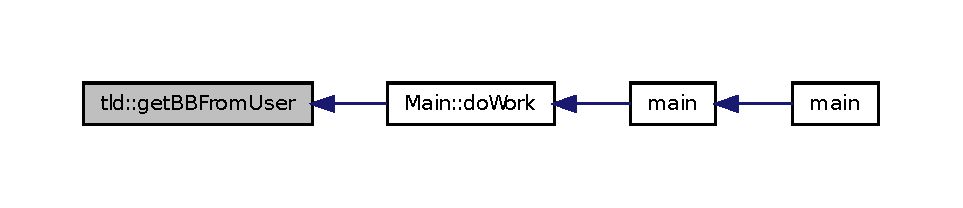
\includegraphics[width=400pt]{namespacetld_a75cd208f8053ece69d5d7de9c2ed33fd_icgraph}
\end{center}
\end{figure}


\hypertarget{namespacetld_a5b279570cd95fb0067a41b5a222e2642}{
\index{tld@{tld}!getopt@{getopt}}
\index{getopt@{getopt}!tld@{tld}}
\subsubsection[{getopt}]{\setlength{\rightskip}{0pt plus 5cm}int tld::getopt (
\begin{DoxyParamCaption}
\item[{int}]{ argc, }
\item[{char $\ast$$\ast$}]{ argv, }
\item[{char $\ast$}]{ opts}
\end{DoxyParamCaption}
)}}
\label{namespacetld_a5b279570cd95fb0067a41b5a222e2642}


Here is the caller graph for this function:
\nopagebreak
\begin{figure}[H]
\begin{center}
\leavevmode
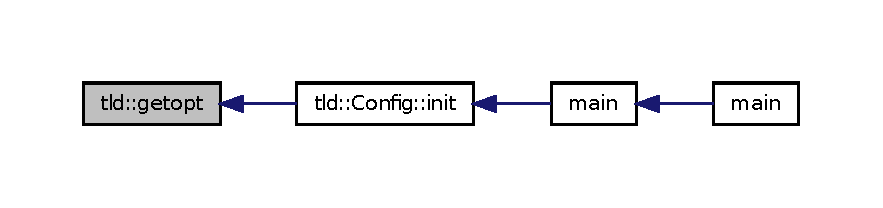
\includegraphics[width=400pt]{namespacetld_a5b279570cd95fb0067a41b5a222e2642_icgraph}
\end{center}
\end{figure}


\hypertarget{namespacetld_a8f2edbadab9bc04731c73571340969a9}{
\index{tld@{tld}!tldArrayToRect@{tldArrayToRect}}
\index{tldArrayToRect@{tldArrayToRect}!tld@{tld}}
\subsubsection[{tldArrayToRect}]{\setlength{\rightskip}{0pt plus 5cm}template$<$class T $>$ cv::Rect tld::tldArrayToRect (
\begin{DoxyParamCaption}
\item[{T $\ast$}]{ boundary}
\end{DoxyParamCaption}
)}}
\label{namespacetld_a8f2edbadab9bc04731c73571340969a9}


Here is the caller graph for this function:
\nopagebreak
\begin{figure}[H]
\begin{center}
\leavevmode
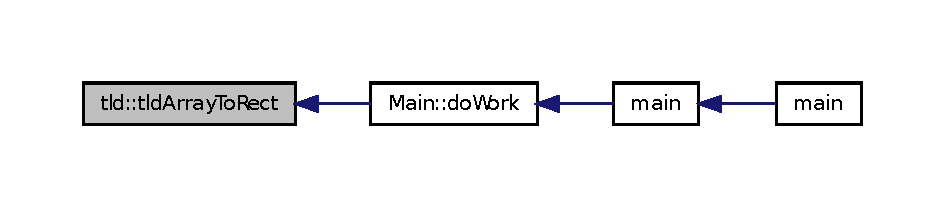
\includegraphics[width=400pt]{namespacetld_a8f2edbadab9bc04731c73571340969a9_icgraph}
\end{center}
\end{figure}


\hypertarget{namespacetld_a19776566a098d3b1fb15030e945a8c14}{
\index{tld@{tld}!tldBBOverlap@{tldBBOverlap}}
\index{tldBBOverlap@{tldBBOverlap}!tld@{tld}}
\subsubsection[{tldBBOverlap}]{\setlength{\rightskip}{0pt plus 5cm}float tld::tldBBOverlap (
\begin{DoxyParamCaption}
\item[{int $\ast$}]{ bb1, }
\item[{int $\ast$}]{ bb2}
\end{DoxyParamCaption}
)}}
\label{namespacetld_a19776566a098d3b1fb15030e945a8c14}


Here is the caller graph for this function:
\nopagebreak
\begin{figure}[H]
\begin{center}
\leavevmode
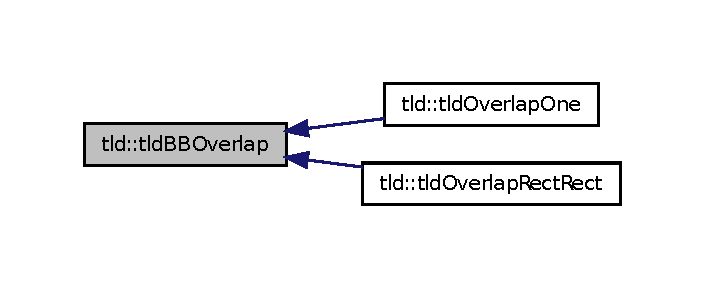
\includegraphics[width=338pt]{namespacetld_a19776566a098d3b1fb15030e945a8c14_icgraph}
\end{center}
\end{figure}


\hypertarget{namespacetld_afd43d8a27c419d1f5da8718be917d4b5}{
\index{tld@{tld}!tldBoundaryToRect@{tldBoundaryToRect}}
\index{tldBoundaryToRect@{tldBoundaryToRect}!tld@{tld}}
\subsubsection[{tldBoundaryToRect}]{\setlength{\rightskip}{0pt plus 5cm}CvRect tld::tldBoundaryToRect (
\begin{DoxyParamCaption}
\item[{int $\ast$}]{ boundary}
\end{DoxyParamCaption}
)}}
\label{namespacetld_afd43d8a27c419d1f5da8718be917d4b5}


Here is the caller graph for this function:
\nopagebreak
\begin{figure}[H]
\begin{center}
\leavevmode
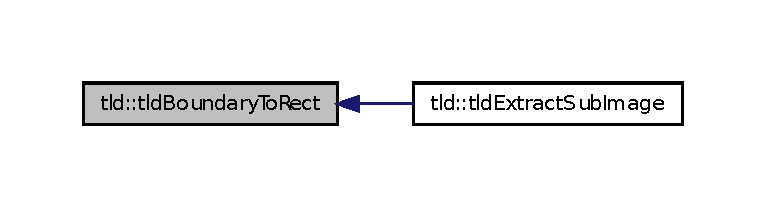
\includegraphics[width=368pt]{namespacetld_afd43d8a27c419d1f5da8718be917d4b5_icgraph}
\end{center}
\end{figure}


\hypertarget{namespacetld_ac0065f4088098aca6e1edd49b2b0f9d3}{
\index{tld@{tld}!tldCalcMean@{tldCalcMean}}
\index{tldCalcMean@{tldCalcMean}!tld@{tld}}
\subsubsection[{tldCalcMean}]{\setlength{\rightskip}{0pt plus 5cm}float tld::tldCalcMean (
\begin{DoxyParamCaption}
\item[{float $\ast$}]{ value, }
\item[{int}]{ n}
\end{DoxyParamCaption}
)}}
\label{namespacetld_ac0065f4088098aca6e1edd49b2b0f9d3}
\hypertarget{namespacetld_a53d4a014fd3df2b3e8a3026a1c1768a7}{
\index{tld@{tld}!tldCalcVariance@{tldCalcVariance}}
\index{tldCalcVariance@{tldCalcVariance}!tld@{tld}}
\subsubsection[{tldCalcVariance}]{\setlength{\rightskip}{0pt plus 5cm}float tld::tldCalcVariance (
\begin{DoxyParamCaption}
\item[{float $\ast$}]{ value, }
\item[{int}]{ n}
\end{DoxyParamCaption}
)}}
\label{namespacetld_a53d4a014fd3df2b3e8a3026a1c1768a7}
\hypertarget{namespacetld_add9262bbbd3c30e3b3bf213e9db13eaf}{
\index{tld@{tld}!tldConvertBB@{tldConvertBB}}
\index{tldConvertBB@{tldConvertBB}!tld@{tld}}
\subsubsection[{tldConvertBB}]{\setlength{\rightskip}{0pt plus 5cm}template$<$class T1 , class T2 $>$ void tld::tldConvertBB (
\begin{DoxyParamCaption}
\item[{T1 $\ast$}]{ src, }
\item[{T2 $\ast$}]{ dest}
\end{DoxyParamCaption}
)}}
\label{namespacetld_add9262bbbd3c30e3b3bf213e9db13eaf}
\hypertarget{namespacetld_a30509a7fb73b21f5006046344ffab792}{
\index{tld@{tld}!tldCopyBB@{tldCopyBB}}
\index{tldCopyBB@{tldCopyBB}!tld@{tld}}
\subsubsection[{tldCopyBB}]{\setlength{\rightskip}{0pt plus 5cm}template$<$class T $>$ void tld::tldCopyBB (
\begin{DoxyParamCaption}
\item[{T $\ast$}]{ src, }
\item[{T $\ast$}]{ dest}
\end{DoxyParamCaption}
)}}
\label{namespacetld_a30509a7fb73b21f5006046344ffab792}
\hypertarget{namespacetld_a8ea4baf48c6ac8c9fc11d0aa36c612e3}{
\index{tld@{tld}!tldCopyBoundaryToArray@{tldCopyBoundaryToArray}}
\index{tldCopyBoundaryToArray@{tldCopyBoundaryToArray}!tld@{tld}}
\subsubsection[{tldCopyBoundaryToArray}]{\setlength{\rightskip}{0pt plus 5cm}template$<$class T $>$ void tld::tldCopyBoundaryToArray (
\begin{DoxyParamCaption}
\item[{T}]{ x, }
\item[{T}]{ y, }
\item[{T}]{ width, }
\item[{T}]{ height, }
\item[{T $\ast$}]{ array}
\end{DoxyParamCaption}
)}}
\label{namespacetld_a8ea4baf48c6ac8c9fc11d0aa36c612e3}
\hypertarget{namespacetld_a41fd3532bec99e023ff75b4706632182}{
\index{tld@{tld}!tldCopyRect@{tldCopyRect}}
\index{tldCopyRect@{tldCopyRect}!tld@{tld}}
\subsubsection[{tldCopyRect}]{\setlength{\rightskip}{0pt plus 5cm}cv::Rect$\ast$ tld::tldCopyRect (
\begin{DoxyParamCaption}
\item[{cv::Rect $\ast$}]{ r}
\end{DoxyParamCaption}
)}}
\label{namespacetld_a41fd3532bec99e023ff75b4706632182}
\hypertarget{namespacetld_a05ea18fc911b12873acd2211f83689f7}{
\index{tld@{tld}!tldCopyRect@{tldCopyRect}}
\index{tldCopyRect@{tldCopyRect}!tld@{tld}}
\subsubsection[{tldCopyRect}]{\setlength{\rightskip}{0pt plus 5cm}Rect$\ast$ tld::tldCopyRect (
\begin{DoxyParamCaption}
\item[{Rect $\ast$}]{ r}
\end{DoxyParamCaption}
)}}
\label{namespacetld_a05ea18fc911b12873acd2211f83689f7}
\hypertarget{namespacetld_aa675c63accc23d4c92133be7f5d93f1f}{
\index{tld@{tld}!tldExtractDimsFromArray@{tldExtractDimsFromArray}}
\index{tldExtractDimsFromArray@{tldExtractDimsFromArray}!tld@{tld}}
\subsubsection[{tldExtractDimsFromArray}]{\setlength{\rightskip}{0pt plus 5cm}template$<$class T $>$ void tld::tldExtractDimsFromArray (
\begin{DoxyParamCaption}
\item[{T $\ast$}]{ boundary, }
\item[{T $\ast$}]{ x, }
\item[{T $\ast$}]{ y, }
\item[{T $\ast$}]{ width, }
\item[{T $\ast$}]{ height}
\end{DoxyParamCaption}
)}}
\label{namespacetld_aa675c63accc23d4c92133be7f5d93f1f}


Here is the caller graph for this function:
\nopagebreak
\begin{figure}[H]
\begin{center}
\leavevmode
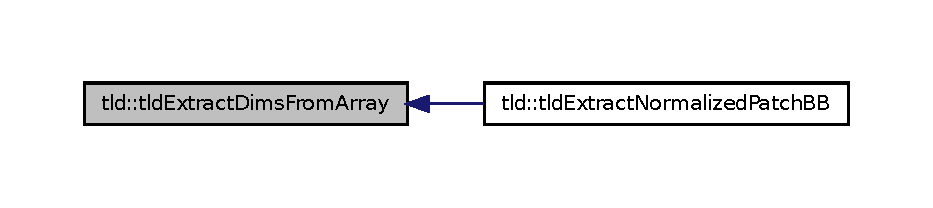
\includegraphics[width=400pt]{namespacetld_aa675c63accc23d4c92133be7f5d93f1f_icgraph}
\end{center}
\end{figure}


\hypertarget{namespacetld_a1bf69e140ab91bdd7bfc794a93a1a096}{
\index{tld@{tld}!tldExtractNormalizedPatch@{tldExtractNormalizedPatch}}
\index{tldExtractNormalizedPatch@{tldExtractNormalizedPatch}!tld@{tld}}
\subsubsection[{tldExtractNormalizedPatch}]{\setlength{\rightskip}{0pt plus 5cm}void tld::tldExtractNormalizedPatch (
\begin{DoxyParamCaption}
\item[{const Mat \&}]{ img, }
\item[{int}]{ x, }
\item[{int}]{ y, }
\item[{int}]{ w, }
\item[{int}]{ h, }
\item[{float $\ast$}]{ output}
\end{DoxyParamCaption}
)}}
\label{namespacetld_a1bf69e140ab91bdd7bfc794a93a1a096}


Here is the call graph for this function:
\nopagebreak
\begin{figure}[H]
\begin{center}
\leavevmode
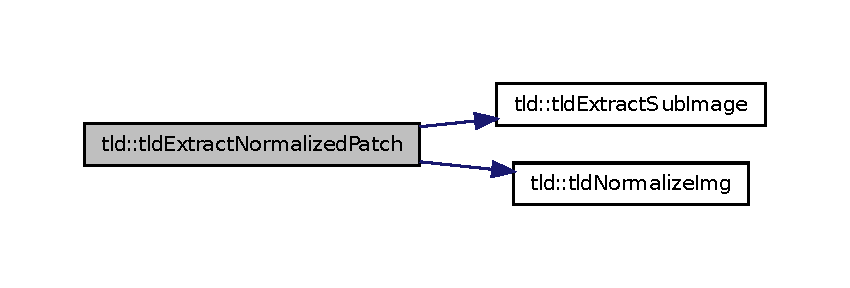
\includegraphics[width=400pt]{namespacetld_a1bf69e140ab91bdd7bfc794a93a1a096_cgraph}
\end{center}
\end{figure}




Here is the caller graph for this function:
\nopagebreak
\begin{figure}[H]
\begin{center}
\leavevmode
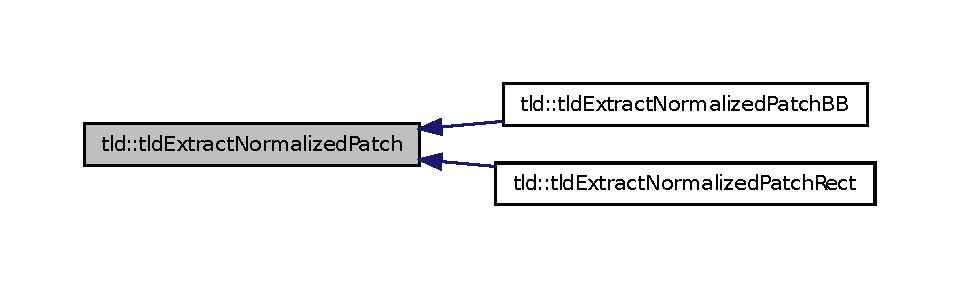
\includegraphics[width=400pt]{namespacetld_a1bf69e140ab91bdd7bfc794a93a1a096_icgraph}
\end{center}
\end{figure}


\hypertarget{namespacetld_ac965be65b1eae7ec666c3bfbe9da065e}{
\index{tld@{tld}!tldExtractNormalizedPatch@{tldExtractNormalizedPatch}}
\index{tldExtractNormalizedPatch@{tldExtractNormalizedPatch}!tld@{tld}}
\subsubsection[{tldExtractNormalizedPatch}]{\setlength{\rightskip}{0pt plus 5cm}void tld::tldExtractNormalizedPatch (
\begin{DoxyParamCaption}
\item[{const cv::Mat \&}]{ img, }
\item[{int}]{ x, }
\item[{int}]{ y, }
\item[{int}]{ w, }
\item[{int}]{ h, }
\item[{float $\ast$}]{ output}
\end{DoxyParamCaption}
)}}
\label{namespacetld_ac965be65b1eae7ec666c3bfbe9da065e}
\hypertarget{namespacetld_adf30e26ca7073712ac0eae4a1f1136ba}{
\index{tld@{tld}!tldExtractNormalizedPatchBB@{tldExtractNormalizedPatchBB}}
\index{tldExtractNormalizedPatchBB@{tldExtractNormalizedPatchBB}!tld@{tld}}
\subsubsection[{tldExtractNormalizedPatchBB}]{\setlength{\rightskip}{0pt plus 5cm}void tld::tldExtractNormalizedPatchBB (
\begin{DoxyParamCaption}
\item[{const Mat \&}]{ img, }
\item[{int $\ast$}]{ boundary, }
\item[{float $\ast$}]{ output}
\end{DoxyParamCaption}
)}}
\label{namespacetld_adf30e26ca7073712ac0eae4a1f1136ba}


Here is the call graph for this function:
\nopagebreak
\begin{figure}[H]
\begin{center}
\leavevmode
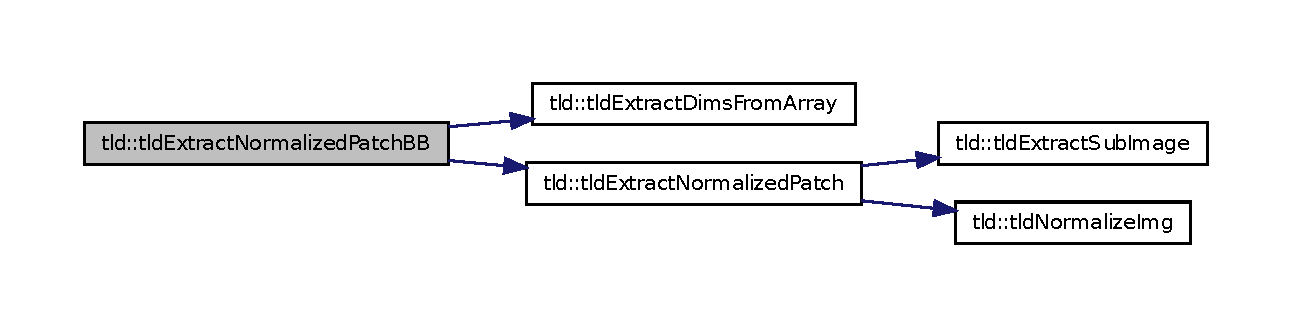
\includegraphics[width=400pt]{namespacetld_adf30e26ca7073712ac0eae4a1f1136ba_cgraph}
\end{center}
\end{figure}


\hypertarget{namespacetld_a44b5f4d4d087d3369129bdc92e2a555a}{
\index{tld@{tld}!tldExtractNormalizedPatchBB@{tldExtractNormalizedPatchBB}}
\index{tldExtractNormalizedPatchBB@{tldExtractNormalizedPatchBB}!tld@{tld}}
\subsubsection[{tldExtractNormalizedPatchBB}]{\setlength{\rightskip}{0pt plus 5cm}void tld::tldExtractNormalizedPatchBB (
\begin{DoxyParamCaption}
\item[{const cv::Mat \&}]{ img, }
\item[{int $\ast$}]{ boundary, }
\item[{float $\ast$}]{ output}
\end{DoxyParamCaption}
)}}
\label{namespacetld_a44b5f4d4d087d3369129bdc92e2a555a}
\hypertarget{namespacetld_aa6c803037b38609e1fceadbb2ad8a75c}{
\index{tld@{tld}!tldExtractNormalizedPatchRect@{tldExtractNormalizedPatchRect}}
\index{tldExtractNormalizedPatchRect@{tldExtractNormalizedPatchRect}!tld@{tld}}
\subsubsection[{tldExtractNormalizedPatchRect}]{\setlength{\rightskip}{0pt plus 5cm}void tld::tldExtractNormalizedPatchRect (
\begin{DoxyParamCaption}
\item[{const cv::Mat \&}]{ img, }
\item[{cv::Rect $\ast$}]{ rect, }
\item[{float $\ast$}]{ output}
\end{DoxyParamCaption}
)}}
\label{namespacetld_aa6c803037b38609e1fceadbb2ad8a75c}
\hypertarget{namespacetld_a7bbab27cff309fae59b25b37268c22d4}{
\index{tld@{tld}!tldExtractNormalizedPatchRect@{tldExtractNormalizedPatchRect}}
\index{tldExtractNormalizedPatchRect@{tldExtractNormalizedPatchRect}!tld@{tld}}
\subsubsection[{tldExtractNormalizedPatchRect}]{\setlength{\rightskip}{0pt plus 5cm}void tld::tldExtractNormalizedPatchRect (
\begin{DoxyParamCaption}
\item[{const Mat \&}]{ img, }
\item[{Rect $\ast$}]{ rect, }
\item[{float $\ast$}]{ output}
\end{DoxyParamCaption}
)}}
\label{namespacetld_a7bbab27cff309fae59b25b37268c22d4}


Here is the call graph for this function:
\nopagebreak
\begin{figure}[H]
\begin{center}
\leavevmode
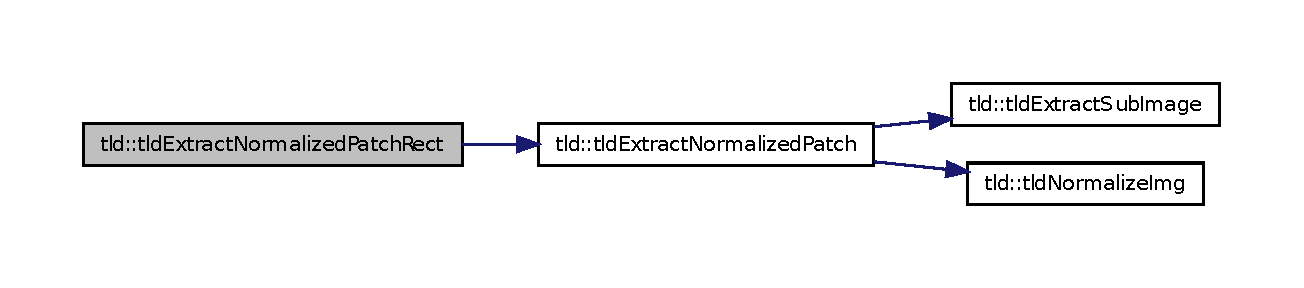
\includegraphics[width=400pt]{namespacetld_a7bbab27cff309fae59b25b37268c22d4_cgraph}
\end{center}
\end{figure}


\hypertarget{namespacetld_a7699b7dc20502fc6d7c5c6c6cbd4be7b}{
\index{tld@{tld}!tldExtractSubImage@{tldExtractSubImage}}
\index{tldExtractSubImage@{tldExtractSubImage}!tld@{tld}}
\subsubsection[{tldExtractSubImage}]{\setlength{\rightskip}{0pt plus 5cm}void tld::tldExtractSubImage (
\begin{DoxyParamCaption}
\item[{const cv::Mat \&}]{ img, }
\item[{cv::Mat \&}]{ subImage, }
\item[{int}]{ x, }
\item[{int}]{ y, }
\item[{int}]{ w, }
\item[{int}]{ h}
\end{DoxyParamCaption}
)}}
\label{namespacetld_a7699b7dc20502fc6d7c5c6c6cbd4be7b}
\hypertarget{namespacetld_a4af40ddc19d189513b3f34f6625eb04f}{
\index{tld@{tld}!tldExtractSubImage@{tldExtractSubImage}}
\index{tldExtractSubImage@{tldExtractSubImage}!tld@{tld}}
\subsubsection[{tldExtractSubImage}]{\setlength{\rightskip}{0pt plus 5cm}void tld::tldExtractSubImage (
\begin{DoxyParamCaption}
\item[{const Mat \&}]{ img, }
\item[{Mat \&}]{ subImage, }
\item[{int $\ast$}]{ boundary}
\end{DoxyParamCaption}
)}}
\label{namespacetld_a4af40ddc19d189513b3f34f6625eb04f}


Here is the call graph for this function:
\nopagebreak
\begin{figure}[H]
\begin{center}
\leavevmode
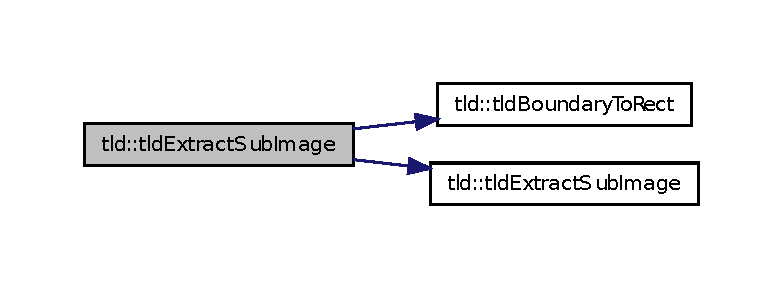
\includegraphics[width=376pt]{namespacetld_a4af40ddc19d189513b3f34f6625eb04f_cgraph}
\end{center}
\end{figure}


\hypertarget{namespacetld_a200bdf631ed45b6d0875996d2e4709f2}{
\index{tld@{tld}!tldExtractSubImage@{tldExtractSubImage}}
\index{tldExtractSubImage@{tldExtractSubImage}!tld@{tld}}
\subsubsection[{tldExtractSubImage}]{\setlength{\rightskip}{0pt plus 5cm}void tld::tldExtractSubImage (
\begin{DoxyParamCaption}
\item[{const Mat \&}]{ img, }
\item[{Mat \&}]{ subImage, }
\item[{CvRect}]{ rect}
\end{DoxyParamCaption}
)}}
\label{namespacetld_a200bdf631ed45b6d0875996d2e4709f2}


Here is the caller graph for this function:
\nopagebreak
\begin{figure}[H]
\begin{center}
\leavevmode
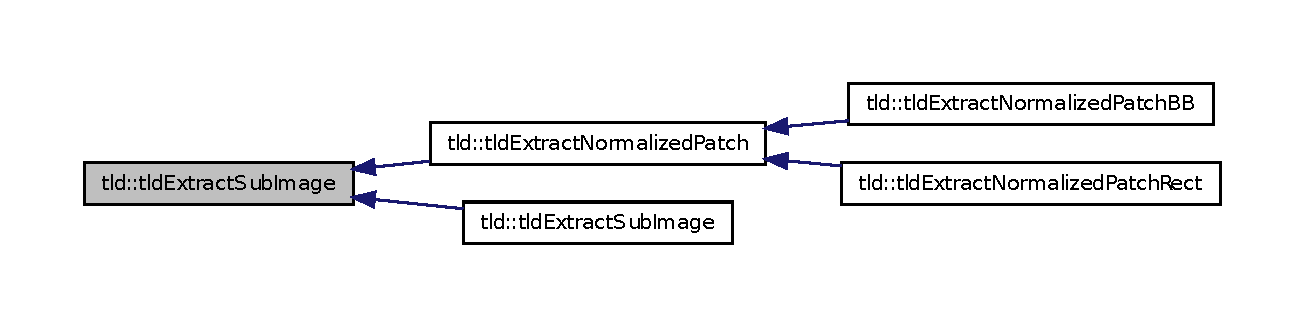
\includegraphics[width=400pt]{namespacetld_a200bdf631ed45b6d0875996d2e4709f2_icgraph}
\end{center}
\end{figure}


\hypertarget{namespacetld_a16fe2b016494fa66be611f723ed7bebc}{
\index{tld@{tld}!tldExtractSubImage@{tldExtractSubImage}}
\index{tldExtractSubImage@{tldExtractSubImage}!tld@{tld}}
\subsubsection[{tldExtractSubImage}]{\setlength{\rightskip}{0pt plus 5cm}void tld::tldExtractSubImage (
\begin{DoxyParamCaption}
\item[{const cv::Mat \&}]{ img, }
\item[{cv::Mat \&}]{ subImage, }
\item[{int $\ast$}]{ boundary}
\end{DoxyParamCaption}
)}}
\label{namespacetld_a16fe2b016494fa66be611f723ed7bebc}
\hypertarget{namespacetld_a8b28e6d4868ad30e826a6248dd2ae7a0}{
\index{tld@{tld}!tldIsInside@{tldIsInside}}
\index{tldIsInside@{tldIsInside}!tld@{tld}}
\subsubsection[{tldIsInside}]{\setlength{\rightskip}{0pt plus 5cm}int tld::tldIsInside (
\begin{DoxyParamCaption}
\item[{int $\ast$}]{ bb1, }
\item[{int $\ast$}]{ bb2}
\end{DoxyParamCaption}
)}}
\label{namespacetld_a8b28e6d4868ad30e826a6248dd2ae7a0}
\hypertarget{namespacetld_a87d078ec7492f2a2a4ef8856abaf6881}{
\index{tld@{tld}!tldNormalizeImg@{tldNormalizeImg}}
\index{tldNormalizeImg@{tldNormalizeImg}!tld@{tld}}
\subsubsection[{tldNormalizeImg}]{\setlength{\rightskip}{0pt plus 5cm}void tld::tldNormalizeImg (
\begin{DoxyParamCaption}
\item[{const Mat \&}]{ img, }
\item[{float $\ast$}]{ output}
\end{DoxyParamCaption}
)}}
\label{namespacetld_a87d078ec7492f2a2a4ef8856abaf6881}


Here is the caller graph for this function:
\nopagebreak
\begin{figure}[H]
\begin{center}
\leavevmode
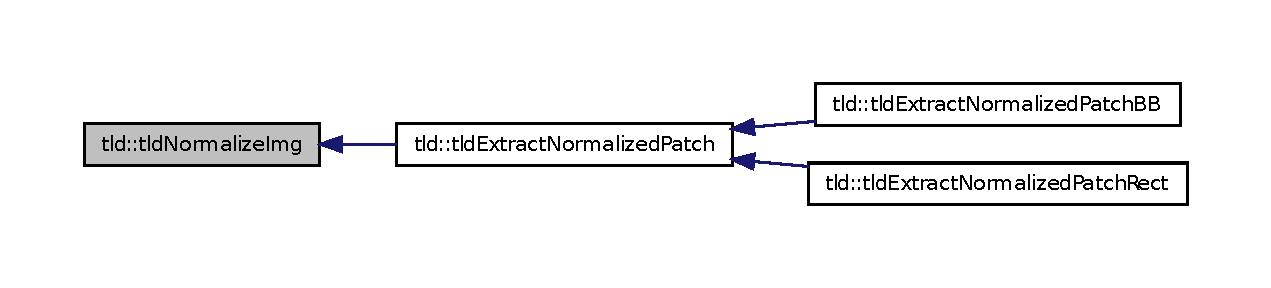
\includegraphics[width=400pt]{namespacetld_a87d078ec7492f2a2a4ef8856abaf6881_icgraph}
\end{center}
\end{figure}


\hypertarget{namespacetld_a52701d320c58fc890fc8e6321aaae61c}{
\index{tld@{tld}!tldNormalizeImg@{tldNormalizeImg}}
\index{tldNormalizeImg@{tldNormalizeImg}!tld@{tld}}
\subsubsection[{tldNormalizeImg}]{\setlength{\rightskip}{0pt plus 5cm}void tld::tldNormalizeImg (
\begin{DoxyParamCaption}
\item[{const cv::Mat \&}]{ img, }
\item[{float $\ast$}]{ result, }
\item[{int}]{ size}
\end{DoxyParamCaption}
)}}
\label{namespacetld_a52701d320c58fc890fc8e6321aaae61c}
\hypertarget{namespacetld_aa9470de30170cb8b3f877dcae45df1b1}{
\index{tld@{tld}!tldOverlap@{tldOverlap}}
\index{tldOverlap@{tldOverlap}!tld@{tld}}
\subsubsection[{tldOverlap}]{\setlength{\rightskip}{0pt plus 5cm}void tld::tldOverlap (
\begin{DoxyParamCaption}
\item[{int $\ast$}]{ windows, }
\item[{int}]{ numWindows, }
\item[{int $\ast$}]{ boundary, }
\item[{float $\ast$}]{ overlap}
\end{DoxyParamCaption}
)}}
\label{namespacetld_aa9470de30170cb8b3f877dcae45df1b1}


Here is the caller graph for this function:
\nopagebreak
\begin{figure}[H]
\begin{center}
\leavevmode
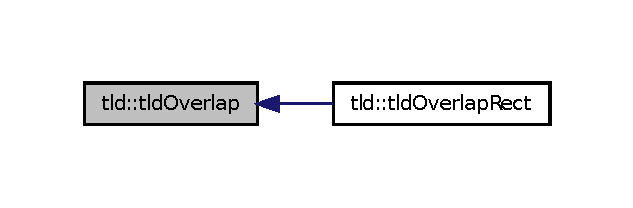
\includegraphics[width=304pt]{namespacetld_aa9470de30170cb8b3f877dcae45df1b1_icgraph}
\end{center}
\end{figure}


\hypertarget{namespacetld_a6db9360f372b596337a075a09b715ee4}{
\index{tld@{tld}!tldOverlapOne@{tldOverlapOne}}
\index{tldOverlapOne@{tldOverlapOne}!tld@{tld}}
\subsubsection[{tldOverlapOne}]{\setlength{\rightskip}{0pt plus 5cm}void tld::tldOverlapOne (
\begin{DoxyParamCaption}
\item[{int $\ast$}]{ windows, }
\item[{int}]{ numWindows, }
\item[{int}]{ index, }
\item[{vector$<$ int $>$ $\ast$}]{ indices, }
\item[{float $\ast$}]{ overlap}
\end{DoxyParamCaption}
)}}
\label{namespacetld_a6db9360f372b596337a075a09b715ee4}


Here is the call graph for this function:
\nopagebreak
\begin{figure}[H]
\begin{center}
\leavevmode
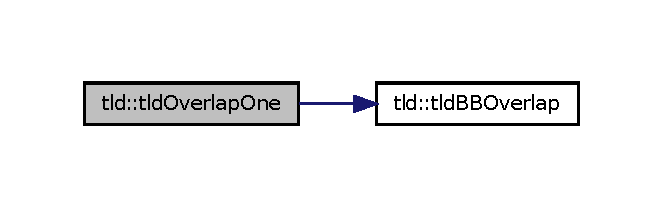
\includegraphics[width=318pt]{namespacetld_a6db9360f372b596337a075a09b715ee4_cgraph}
\end{center}
\end{figure}


\hypertarget{namespacetld_a018caa7bf4a554814fe61a679a219489}{
\index{tld@{tld}!tldOverlapOne@{tldOverlapOne}}
\index{tldOverlapOne@{tldOverlapOne}!tld@{tld}}
\subsubsection[{tldOverlapOne}]{\setlength{\rightskip}{0pt plus 5cm}void tld::tldOverlapOne (
\begin{DoxyParamCaption}
\item[{int $\ast$}]{ windows, }
\item[{int}]{ numWindows, }
\item[{int}]{ index, }
\item[{std::vector$<$ int $>$ $\ast$}]{ indices, }
\item[{float $\ast$}]{ overlap}
\end{DoxyParamCaption}
)}}
\label{namespacetld_a018caa7bf4a554814fe61a679a219489}
\hypertarget{namespacetld_ab71405a293095380c793589e8d59d4c7}{
\index{tld@{tld}!tldOverlapRect@{tldOverlapRect}}
\index{tldOverlapRect@{tldOverlapRect}!tld@{tld}}
\subsubsection[{tldOverlapRect}]{\setlength{\rightskip}{0pt plus 5cm}void tld::tldOverlapRect (
\begin{DoxyParamCaption}
\item[{int $\ast$}]{ windows, }
\item[{int}]{ numWindows, }
\item[{Rect $\ast$}]{ boundary, }
\item[{float $\ast$}]{ overlap}
\end{DoxyParamCaption}
)}}
\label{namespacetld_ab71405a293095380c793589e8d59d4c7}


Here is the call graph for this function:
\nopagebreak
\begin{figure}[H]
\begin{center}
\leavevmode
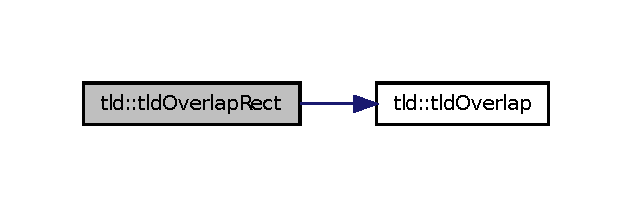
\includegraphics[width=304pt]{namespacetld_ab71405a293095380c793589e8d59d4c7_cgraph}
\end{center}
\end{figure}


\hypertarget{namespacetld_ae87c7dbe6b4da1e1923c42bec18caaf6}{
\index{tld@{tld}!tldOverlapRect@{tldOverlapRect}}
\index{tldOverlapRect@{tldOverlapRect}!tld@{tld}}
\subsubsection[{tldOverlapRect}]{\setlength{\rightskip}{0pt plus 5cm}void tld::tldOverlapRect (
\begin{DoxyParamCaption}
\item[{int $\ast$}]{ windows, }
\item[{int}]{ numWindows, }
\item[{cv::Rect $\ast$}]{ boundary, }
\item[{float $\ast$}]{ overlap}
\end{DoxyParamCaption}
)}}
\label{namespacetld_ae87c7dbe6b4da1e1923c42bec18caaf6}
\hypertarget{namespacetld_afdab54607fed863cdc408f72fd0f774b}{
\index{tld@{tld}!tldOverlapRectRect@{tldOverlapRectRect}}
\index{tldOverlapRectRect@{tldOverlapRectRect}!tld@{tld}}
\subsubsection[{tldOverlapRectRect}]{\setlength{\rightskip}{0pt plus 5cm}float tld::tldOverlapRectRect (
\begin{DoxyParamCaption}
\item[{cv::Rect}]{ r1, }
\item[{cv::Rect}]{ r2}
\end{DoxyParamCaption}
)}}
\label{namespacetld_afdab54607fed863cdc408f72fd0f774b}
\hypertarget{namespacetld_afe4210f75b17cb13bb95c8d4c08a543a}{
\index{tld@{tld}!tldOverlapRectRect@{tldOverlapRectRect}}
\index{tldOverlapRectRect@{tldOverlapRectRect}!tld@{tld}}
\subsubsection[{tldOverlapRectRect}]{\setlength{\rightskip}{0pt plus 5cm}float tld::tldOverlapRectRect (
\begin{DoxyParamCaption}
\item[{Rect}]{ r1, }
\item[{Rect}]{ r2}
\end{DoxyParamCaption}
)}}
\label{namespacetld_afe4210f75b17cb13bb95c8d4c08a543a}


Here is the call graph for this function:
\nopagebreak
\begin{figure}[H]
\begin{center}
\leavevmode
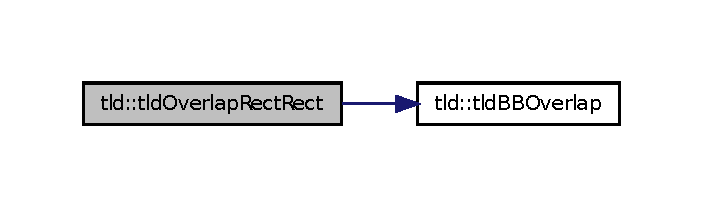
\includegraphics[width=338pt]{namespacetld_afe4210f75b17cb13bb95c8d4c08a543a_cgraph}
\end{center}
\end{figure}


\hypertarget{namespacetld_acca496d96df1e566f1a08bebb7e75f1c}{
\index{tld@{tld}!tldRectToArray@{tldRectToArray}}
\index{tldRectToArray@{tldRectToArray}!tld@{tld}}
\subsubsection[{tldRectToArray}]{\setlength{\rightskip}{0pt plus 5cm}template$<$class T $>$ void tld::tldRectToArray (
\begin{DoxyParamCaption}
\item[{cv::Rect}]{ rect, }
\item[{T $\ast$}]{ boundary}
\end{DoxyParamCaption}
)}}
\label{namespacetld_acca496d96df1e566f1a08bebb7e75f1c}
\hypertarget{namespacetld_a1899d52f23a94a9042fb95249b4714ba}{
\index{tld@{tld}!tldSortByOverlapDesc@{tldSortByOverlapDesc}}
\index{tldSortByOverlapDesc@{tldSortByOverlapDesc}!tld@{tld}}
\subsubsection[{tldSortByOverlapDesc}]{\setlength{\rightskip}{0pt plus 5cm}bool tld::tldSortByOverlapDesc (
\begin{DoxyParamCaption}
\item[{pair$<$ int, float $>$}]{ bb1, }
\item[{pair$<$ int, float $>$}]{ bb2}
\end{DoxyParamCaption}
)}}
\label{namespacetld_a1899d52f23a94a9042fb95249b4714ba}
\hypertarget{namespacetld_acaf374df081816ecaf9079e200a8f5af}{
\index{tld@{tld}!tldSortByOverlapDesc@{tldSortByOverlapDesc}}
\index{tldSortByOverlapDesc@{tldSortByOverlapDesc}!tld@{tld}}
\subsubsection[{tldSortByOverlapDesc}]{\setlength{\rightskip}{0pt plus 5cm}bool tld::tldSortByOverlapDesc (
\begin{DoxyParamCaption}
\item[{std::pair$<$ int, float $>$}]{ bb1, }
\item[{std::pair$<$ int, float $>$}]{ bb2}
\end{DoxyParamCaption}
)}}
\label{namespacetld_acaf374df081816ecaf9079e200a8f5af}


\subsection{Variable Documentation}
\hypertarget{namespacetld_a1bbc7d3201a2ef41da5495e0e48cfd2e}{
\index{tld@{tld}!optarg@{optarg}}
\index{optarg@{optarg}!tld@{tld}}
\subsubsection[{optarg}]{\setlength{\rightskip}{0pt plus 5cm}char $\ast$ {\bf tld::optarg}}}
\label{namespacetld_a1bbc7d3201a2ef41da5495e0e48cfd2e}
\hypertarget{namespacetld_a6e180d5067af278cc277ae9c6f7507c1}{
\index{tld@{tld}!opterr@{opterr}}
\index{opterr@{opterr}!tld@{tld}}
\subsubsection[{opterr}]{\setlength{\rightskip}{0pt plus 5cm}int {\bf tld::opterr} = 1}}
\label{namespacetld_a6e180d5067af278cc277ae9c6f7507c1}
\hypertarget{namespacetld_ab8c5a378ef03678c537edc84a15abc22}{
\index{tld@{tld}!optind@{optind}}
\index{optind@{optind}!tld@{tld}}
\subsubsection[{optind}]{\setlength{\rightskip}{0pt plus 5cm}int {\bf tld::optind} = 1}}
\label{namespacetld_ab8c5a378ef03678c537edc84a15abc22}
\hypertarget{namespacetld_a6d6bd80732b9f396bc03e5f2c5cf30f8}{
\index{tld@{tld}!optopt@{optopt}}
\index{optopt@{optopt}!tld@{tld}}
\subsubsection[{optopt}]{\setlength{\rightskip}{0pt plus 5cm}int {\bf tld::optopt}}}
\label{namespacetld_a6d6bd80732b9f396bc03e5f2c5cf30f8}

\chapter{Class Documentation}
\hypertarget{class_c_blob}{
\section{CBlob Class Reference}
\label{class_c_blob}\index{CBlob@{CBlob}}
}


Blob class.  




{\ttfamily \#include $<$blob.h$>$}



Collaboration diagram for CBlob:
\nopagebreak
\begin{figure}[H]
\begin{center}
\leavevmode
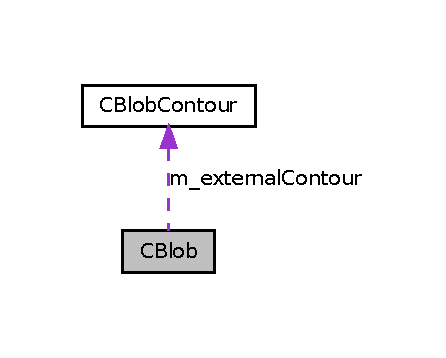
\includegraphics[width=214pt]{class_c_blob__coll__graph}
\end{center}
\end{figure}
\subsection*{Public Member Functions}
\begin{DoxyCompactItemize}
\item 
\hyperlink{class_c_blob_acd24304c1bc98128b24914f3e4bfea7c}{CBlob} ()
\item 
\hyperlink{class_c_blob_a45d7bbe67ef246fe180e16f5a7116c6f}{CBlob} (\hyperlink{blob_8h_ae21ba61a4f023a2f91fc5feaad495073}{t\_\-labelType} id, CvPoint startPoint, CvSize originalImageSize)
\item 
\hyperlink{class_c_blob_a593ffb9ba17290432d04c383f2f104e2}{$\sim$CBlob} ()
\item 
\hyperlink{class_c_blob_af87156ca1ac7f64a860b7cf8c07fd1fa}{CBlob} (const \hyperlink{class_c_blob}{CBlob} \&src)
\begin{DoxyCompactList}\small\item\em Copy constructor. \item\end{DoxyCompactList}\item 
\hyperlink{class_c_blob_a61719b6e5ebff6d3e383b98bce4137dc}{CBlob} (const \hyperlink{class_c_blob}{CBlob} $\ast$src)
\item 
\hyperlink{class_c_blob}{CBlob} \& \hyperlink{class_c_blob_a724e55442a030bf94da856310e324a40}{operator=} (const \hyperlink{class_c_blob}{CBlob} \&src)
\item 
void \hyperlink{class_c_blob_ad26a1bc4e31809c3bd76424b05824e90}{AddInternalContour} (const \hyperlink{class_c_blob_contour}{CBlobContour} \&newContour)
\begin{DoxyCompactList}\small\item\em Adds a new internal contour to the blob. \item\end{DoxyCompactList}\item 
\hyperlink{class_c_blob_contour}{CBlobContour} $\ast$ \hyperlink{class_c_blob_ad136387165bd74c368cb4ecc7632e4cf}{GetExternalContour} ()
\begin{DoxyCompactList}\small\item\em Retrieves contour in Freeman's chain code. \item\end{DoxyCompactList}\item 
CvMemStorage $\ast$ \hyperlink{class_c_blob_a1eeee72a4369dc9485c6ae6573631a02}{GetStorage} ()
\begin{DoxyCompactList}\small\item\em Retrieves blob storage. \item\end{DoxyCompactList}\item 
\hyperlink{blob_8h_ae21ba61a4f023a2f91fc5feaad495073}{t\_\-labelType} \hyperlink{class_c_blob_a1d3fd90bc98f6d845babb18a3f058bc2}{GetID} ()
\begin{DoxyCompactList}\small\item\em Get label ID. \item\end{DoxyCompactList}\item 
int \hyperlink{class_c_blob_a2d56a7dee1cbeb3178ff083630ee31b0}{Exterior} (IplImage $\ast$mask, bool xBorder=true, bool yBorder=true)
\begin{DoxyCompactList}\small\item\em $>$ 0 for extern blobs, 0 if not \item\end{DoxyCompactList}\item 
double \hyperlink{class_c_blob_a6f1db9fcb42c0a3ea003aaeb0ec65a8d}{Area} ()
\begin{DoxyCompactList}\small\item\em Compute blob's area. \item\end{DoxyCompactList}\item 
double \hyperlink{class_c_blob_af63853ea55dbebbee5b013189e765b51}{Perimeter} ()
\begin{DoxyCompactList}\small\item\em Compute blob's perimeter. \item\end{DoxyCompactList}\item 
double \hyperlink{class_c_blob_a4f5dfca1ee933e07a39965375f9f07c5}{Moment} (int p, int q)
\begin{DoxyCompactList}\small\item\em Compute blob's moment (p,q up to MAX\_\-CALCULATED\_\-MOMENTS). \item\end{DoxyCompactList}\item 
double \hyperlink{class_c_blob_ab1501b07a2c5ee23843bac66d20974e2}{ExternPerimeter} (IplImage $\ast$mask, bool xBorder=true, bool yBorder=true)
\begin{DoxyCompactList}\small\item\em Compute extern perimeter. \item\end{DoxyCompactList}\item 
double \hyperlink{class_c_blob_a1b12d25f8e470fdd808ac2e3bfe9bad4}{Mean} (IplImage $\ast$image)
\begin{DoxyCompactList}\small\item\em Get mean grey color. \item\end{DoxyCompactList}\item 
double \hyperlink{class_c_blob_a014b670bb748e6767ef070e1bc25be7a}{StdDev} (IplImage $\ast$image)
\begin{DoxyCompactList}\small\item\em Get standard deviation grey color. \item\end{DoxyCompactList}\item 
bool \hyperlink{class_c_blob_ac97e73d3040530de09a187d02632deb1}{IsEmpty} ()
\item 
\hyperlink{_blob_contour_8h_abf72b29b2c653dd623e9b39a447809c0}{t\_\-PointList} \hyperlink{class_c_blob_aacc50d5d47e0543d4e0a569d05009006}{GetConvexHull} ()
\item 
void \hyperlink{class_c_blob_a1a12b6dee61d2db86cd3a60c0671382e}{FillBlob} (IplImage $\ast$imatge, CvScalar color, int offsetX=0, int offsetY=0)
\item 
void \hyperlink{class_c_blob_a006463cc42ef0e4b8986fa5020cb6f90}{JoinBlob} (\hyperlink{class_c_blob}{CBlob} $\ast$blob)
\begin{DoxyCompactList}\small\item\em Join a blob to current one (add's contour. \item\end{DoxyCompactList}\item 
CvRect \hyperlink{class_c_blob_a5391167c172eb461eb762fbdd81306de}{GetBoundingBox} ()
\begin{DoxyCompactList}\small\item\em Get bounding box. \item\end{DoxyCompactList}\item 
CvBox2D \hyperlink{class_c_blob_ad0bb95f395084ee89ca35cf11f203342}{GetEllipse} ()
\begin{DoxyCompactList}\small\item\em Get bounding ellipse. \item\end{DoxyCompactList}\item 
double \hyperlink{class_c_blob_aa3313af22e7f28d65ba245bc3b8a30bc}{MinX} ()
\begin{DoxyCompactList}\small\item\em Minimun X. \item\end{DoxyCompactList}\item 
double \hyperlink{class_c_blob_a44e2caf6c7fc6e8360d2576c18c9bc2b}{MinY} ()
\begin{DoxyCompactList}\small\item\em Minimun Y. \item\end{DoxyCompactList}\item 
double \hyperlink{class_c_blob_ab26a757fffc581df39620425de008cbc}{MaxX} ()
\begin{DoxyCompactList}\small\item\em Maximun X. \item\end{DoxyCompactList}\item 
double \hyperlink{class_c_blob_a740a37afcd841bf719587d2f0128c555}{MaxY} ()
\begin{DoxyCompactList}\small\item\em Maximun Y. \item\end{DoxyCompactList}\end{DoxyCompactItemize}


\subsection{Detailed Description}
Blob class. 

\subsection{Constructor \& Destructor Documentation}
\hypertarget{class_c_blob_acd24304c1bc98128b24914f3e4bfea7c}{
\index{CBlob@{CBlob}!CBlob@{CBlob}}
\index{CBlob@{CBlob}!CBlob@{CBlob}}
\subsubsection[{CBlob}]{\setlength{\rightskip}{0pt plus 5cm}CBlob::CBlob (
\begin{DoxyParamCaption}
{}
\end{DoxyParamCaption}
)}}
\label{class_c_blob_acd24304c1bc98128b24914f3e4bfea7c}
\hypertarget{class_c_blob_a45d7bbe67ef246fe180e16f5a7116c6f}{
\index{CBlob@{CBlob}!CBlob@{CBlob}}
\index{CBlob@{CBlob}!CBlob@{CBlob}}
\subsubsection[{CBlob}]{\setlength{\rightskip}{0pt plus 5cm}CBlob::CBlob (
\begin{DoxyParamCaption}
\item[{{\bf t\_\-labelType}}]{ id, }
\item[{CvPoint}]{ startPoint, }
\item[{CvSize}]{ originalImageSize}
\end{DoxyParamCaption}
)}}
\label{class_c_blob_a45d7bbe67ef246fe180e16f5a7116c6f}
\hypertarget{class_c_blob_a593ffb9ba17290432d04c383f2f104e2}{
\index{CBlob@{CBlob}!$\sim$CBlob@{$\sim$CBlob}}
\index{$\sim$CBlob@{$\sim$CBlob}!CBlob@{CBlob}}
\subsubsection[{$\sim$CBlob}]{\setlength{\rightskip}{0pt plus 5cm}CBlob::$\sim$CBlob (
\begin{DoxyParamCaption}
{}
\end{DoxyParamCaption}
)}}
\label{class_c_blob_a593ffb9ba17290432d04c383f2f104e2}
\hypertarget{class_c_blob_af87156ca1ac7f64a860b7cf8c07fd1fa}{
\index{CBlob@{CBlob}!CBlob@{CBlob}}
\index{CBlob@{CBlob}!CBlob@{CBlob}}
\subsubsection[{CBlob}]{\setlength{\rightskip}{0pt plus 5cm}CBlob::CBlob (
\begin{DoxyParamCaption}
\item[{const {\bf CBlob} \&}]{ src}
\end{DoxyParamCaption}
)}}
\label{class_c_blob_af87156ca1ac7f64a860b7cf8c07fd1fa}


Copy constructor. 

\hypertarget{class_c_blob_a61719b6e5ebff6d3e383b98bce4137dc}{
\index{CBlob@{CBlob}!CBlob@{CBlob}}
\index{CBlob@{CBlob}!CBlob@{CBlob}}
\subsubsection[{CBlob}]{\setlength{\rightskip}{0pt plus 5cm}CBlob::CBlob (
\begin{DoxyParamCaption}
\item[{const {\bf CBlob} $\ast$}]{ src}
\end{DoxyParamCaption}
)}}
\label{class_c_blob_a61719b6e5ebff6d3e383b98bce4137dc}


\subsection{Member Function Documentation}
\hypertarget{class_c_blob_ad26a1bc4e31809c3bd76424b05824e90}{
\index{CBlob@{CBlob}!AddInternalContour@{AddInternalContour}}
\index{AddInternalContour@{AddInternalContour}!CBlob@{CBlob}}
\subsubsection[{AddInternalContour}]{\setlength{\rightskip}{0pt plus 5cm}void CBlob::AddInternalContour (
\begin{DoxyParamCaption}
\item[{const {\bf CBlobContour} \&}]{ newContour}
\end{DoxyParamCaption}
)}}
\label{class_c_blob_ad26a1bc4e31809c3bd76424b05824e90}


Adds a new internal contour to the blob. 



Here is the caller graph for this function:
\nopagebreak
\begin{figure}[H]
\begin{center}
\leavevmode
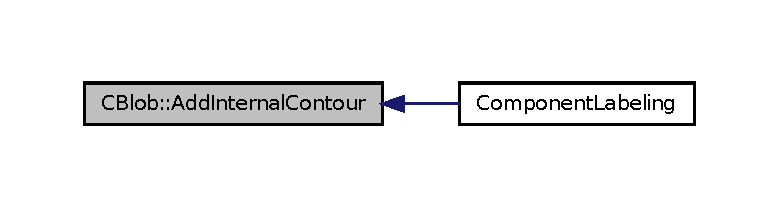
\includegraphics[width=374pt]{class_c_blob_ad26a1bc4e31809c3bd76424b05824e90_icgraph}
\end{center}
\end{figure}


\hypertarget{class_c_blob_a6f1db9fcb42c0a3ea003aaeb0ec65a8d}{
\index{CBlob@{CBlob}!Area@{Area}}
\index{Area@{Area}!CBlob@{CBlob}}
\subsubsection[{Area}]{\setlength{\rightskip}{0pt plus 5cm}double CBlob::Area (
\begin{DoxyParamCaption}
{}
\end{DoxyParamCaption}
)}}
\label{class_c_blob_a6f1db9fcb42c0a3ea003aaeb0ec65a8d}


Compute blob's area. 


\begin{DoxyItemize}
\item FUNCI�: Area
\item FUNCIONALITAT: Get blob area, ie. external contour area minus internal contours area
\item PAR�METRES:
\begin{DoxyItemize}
\item 
\end{DoxyItemize}
\item RESULTAT:
\begin{DoxyItemize}
\item 
\end{DoxyItemize}
\item RESTRICCIONS:
\begin{DoxyItemize}
\item 
\end{DoxyItemize}
\item AUTOR: rborras
\item DATA DE CREACI�: 2008/04/30
\item MODIFICACI�: Data. Autor. Descripci�. 
\end{DoxyItemize}

Here is the call graph for this function:
\nopagebreak
\begin{figure}[H]
\begin{center}
\leavevmode
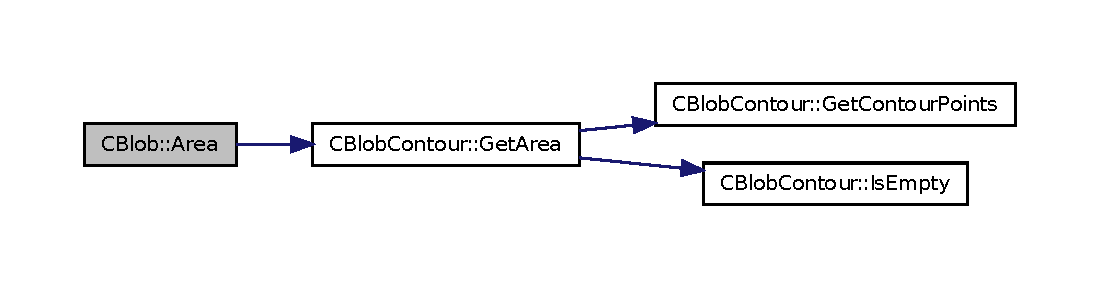
\includegraphics[width=400pt]{class_c_blob_a6f1db9fcb42c0a3ea003aaeb0ec65a8d_cgraph}
\end{center}
\end{figure}




Here is the caller graph for this function:
\nopagebreak
\begin{figure}[H]
\begin{center}
\leavevmode
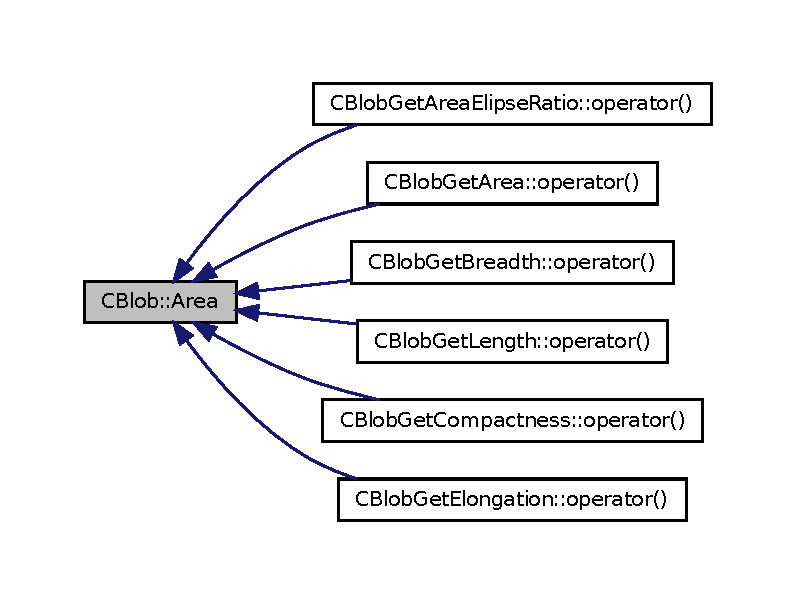
\includegraphics[width=382pt]{class_c_blob_a6f1db9fcb42c0a3ea003aaeb0ec65a8d_icgraph}
\end{center}
\end{figure}


\hypertarget{class_c_blob_a2d56a7dee1cbeb3178ff083630ee31b0}{
\index{CBlob@{CBlob}!Exterior@{Exterior}}
\index{Exterior@{Exterior}!CBlob@{CBlob}}
\subsubsection[{Exterior}]{\setlength{\rightskip}{0pt plus 5cm}int CBlob::Exterior (
\begin{DoxyParamCaption}
\item[{IplImage $\ast$}]{ mask, }
\item[{bool}]{ xBorder = {\ttfamily true}, }
\item[{bool}]{ yBorder = {\ttfamily true}}
\end{DoxyParamCaption}
)}}
\label{class_c_blob_a2d56a7dee1cbeb3178ff083630ee31b0}


$>$ 0 for extern blobs, 0 if not 


\begin{DoxyItemize}
\item FUNCI�: Exterior
\item FUNCIONALITAT: Return true for extern blobs
\item PAR�METRES:
\begin{DoxyItemize}
\item xBorder: true to consider blobs touching horizontal borders as extern
\item yBorder: true to consider blobs touching vertical borders as extern
\end{DoxyItemize}
\item RESULTAT:
\begin{DoxyItemize}
\item 
\end{DoxyItemize}
\item RESTRICCIONS:
\begin{DoxyItemize}
\item 
\end{DoxyItemize}
\item AUTOR: rborras
\item DATA DE CREACI�: 2008/05/06
\item MODIFICACI�: Data. Autor. Descripci�. 
\end{DoxyItemize}

Here is the call graph for this function:
\nopagebreak
\begin{figure}[H]
\begin{center}
\leavevmode
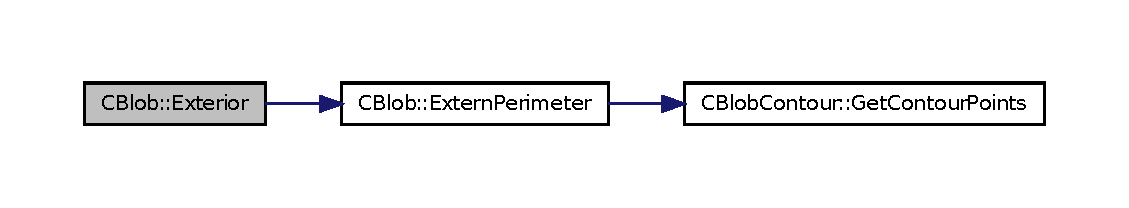
\includegraphics[width=400pt]{class_c_blob_a2d56a7dee1cbeb3178ff083630ee31b0_cgraph}
\end{center}
\end{figure}




Here is the caller graph for this function:
\nopagebreak
\begin{figure}[H]
\begin{center}
\leavevmode
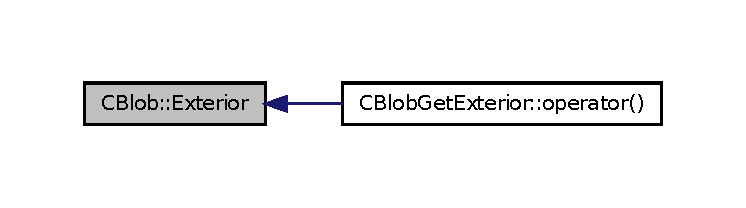
\includegraphics[width=358pt]{class_c_blob_a2d56a7dee1cbeb3178ff083630ee31b0_icgraph}
\end{center}
\end{figure}


\hypertarget{class_c_blob_ab1501b07a2c5ee23843bac66d20974e2}{
\index{CBlob@{CBlob}!ExternPerimeter@{ExternPerimeter}}
\index{ExternPerimeter@{ExternPerimeter}!CBlob@{CBlob}}
\subsubsection[{ExternPerimeter}]{\setlength{\rightskip}{0pt plus 5cm}double CBlob::ExternPerimeter (
\begin{DoxyParamCaption}
\item[{IplImage $\ast$}]{ maskImage, }
\item[{bool}]{ xBorder = {\ttfamily true}, }
\item[{bool}]{ yBorder = {\ttfamily true}}
\end{DoxyParamCaption}
)}}
\label{class_c_blob_ab1501b07a2c5ee23843bac66d20974e2}


Compute extern perimeter. 


\begin{DoxyItemize}
\item FUNCI�: ExternPerimeter
\item FUNCIONALITAT: Get extern perimeter (perimeter touching image borders)
\item PAR�METRES:
\begin{DoxyItemize}
\item maskImage: if != NULL, counts maskImage black pixels as external pixels and contour points touching them are counted as external contour points.
\item xBorder: true to consider blobs touching horizontal borders as extern
\item yBorder: true to consider blobs touching vertical borders as extern
\end{DoxyItemize}
\item RESULTAT:
\begin{DoxyItemize}
\item 
\end{DoxyItemize}
\item RESTRICCIONS:
\begin{DoxyItemize}
\item 
\end{DoxyItemize}
\item AUTOR: rborras
\item DATA DE CREACI�: 2008/05/05
\item MODIFICACI�: Data. Autor. Descripci�.
\item NOTA: If \hyperlink{class_c_blob_contour_a245d5e59180619aa9ae4ec14acc18744}{CBlobContour::GetContourPoints} aproximates contours with a method different that NONE, this function will not give correct results 
\end{DoxyItemize}

Here is the call graph for this function:
\nopagebreak
\begin{figure}[H]
\begin{center}
\leavevmode
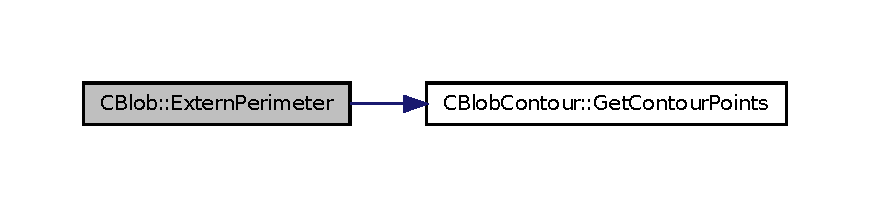
\includegraphics[width=400pt]{class_c_blob_ab1501b07a2c5ee23843bac66d20974e2_cgraph}
\end{center}
\end{figure}




Here is the caller graph for this function:
\nopagebreak
\begin{figure}[H]
\begin{center}
\leavevmode
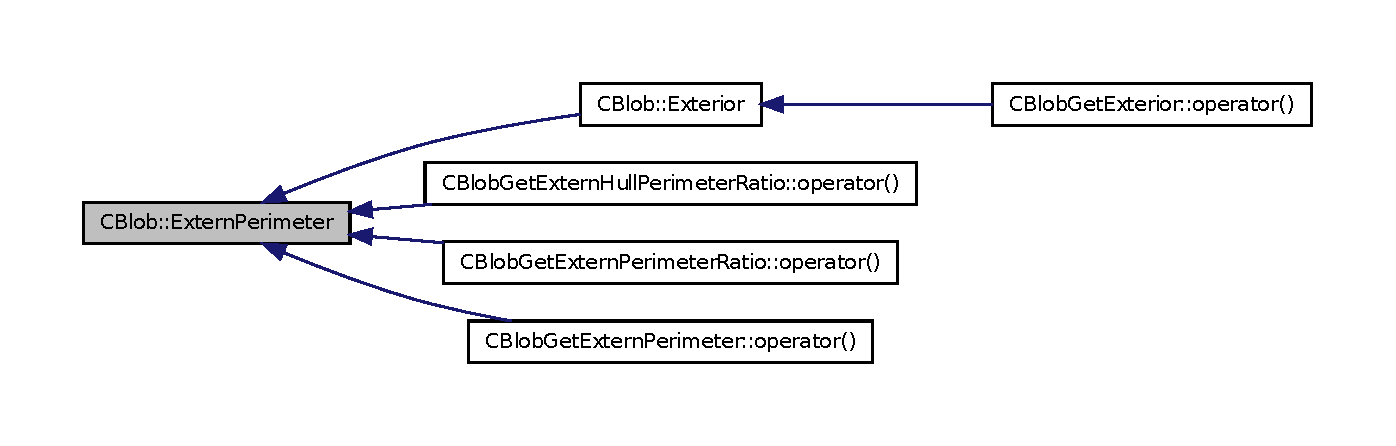
\includegraphics[width=400pt]{class_c_blob_ab1501b07a2c5ee23843bac66d20974e2_icgraph}
\end{center}
\end{figure}


\hypertarget{class_c_blob_a1a12b6dee61d2db86cd3a60c0671382e}{
\index{CBlob@{CBlob}!FillBlob@{FillBlob}}
\index{FillBlob@{FillBlob}!CBlob@{CBlob}}
\subsubsection[{FillBlob}]{\setlength{\rightskip}{0pt plus 5cm}void CBlob::FillBlob (
\begin{DoxyParamCaption}
\item[{IplImage $\ast$}]{ imatge, }
\item[{CvScalar}]{ color, }
\item[{int}]{ offsetX = {\ttfamily 0}, }
\item[{int}]{ offsetY = {\ttfamily 0}}
\end{DoxyParamCaption}
)}}
\label{class_c_blob_a1a12b6dee61d2db86cd3a60c0671382e}
Pinta l'interior d'un blob d'un color determinat Paints the blob in an image


\begin{DoxyItemize}
\item FUNCTION: FillBlob
\item FUNCTIONALITY:
\begin{DoxyItemize}
\item Fills the blob with a specified colour
\end{DoxyItemize}
\item PARAMETERS:
\begin{DoxyItemize}
\item imatge: where to paint
\item color: colour to paint the blob
\end{DoxyItemize}
\item RESULT:
\begin{DoxyItemize}
\item modifies input image and returns the seed point used to fill the blob
\end{DoxyItemize}
\item RESTRICTIONS:
\item AUTHOR: Ricard Borr�s
\item CREATION DATE: 25-\/05-\/2005.
\item MODIFICATION: Date. Author. Description. 
\end{DoxyItemize}

Here is the call graph for this function:
\nopagebreak
\begin{figure}[H]
\begin{center}
\leavevmode
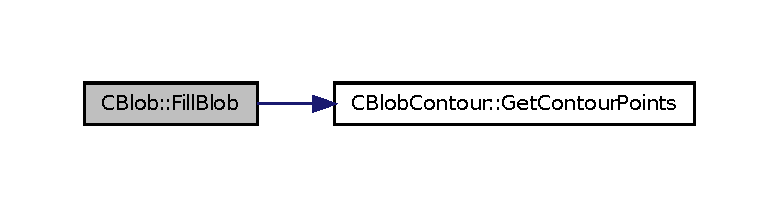
\includegraphics[width=374pt]{class_c_blob_a1a12b6dee61d2db86cd3a60c0671382e_cgraph}
\end{center}
\end{figure}


\hypertarget{class_c_blob_a5391167c172eb461eb762fbdd81306de}{
\index{CBlob@{CBlob}!GetBoundingBox@{GetBoundingBox}}
\index{GetBoundingBox@{GetBoundingBox}!CBlob@{CBlob}}
\subsubsection[{GetBoundingBox}]{\setlength{\rightskip}{0pt plus 5cm}CvRect CBlob::GetBoundingBox (
\begin{DoxyParamCaption}
{}
\end{DoxyParamCaption}
)}}
\label{class_c_blob_a5391167c172eb461eb762fbdd81306de}


Get bounding box. 


\begin{DoxyItemize}
\item FUNCI�: GetBoundingBox
\item FUNCIONALITAT: Get bounding box (without rotation) of a blob
\item PAR�METRES:
\begin{DoxyItemize}
\item 
\end{DoxyItemize}
\item RESULTAT:
\begin{DoxyItemize}
\item 
\end{DoxyItemize}
\item RESTRICCIONS:
\begin{DoxyItemize}
\item 
\end{DoxyItemize}
\item AUTOR: rborras
\item DATA DE CREACI�: 2008/05/06
\item MODIFICACI�: Data. Autor. Descripci�. 
\end{DoxyItemize}

Here is the call graph for this function:
\nopagebreak
\begin{figure}[H]
\begin{center}
\leavevmode
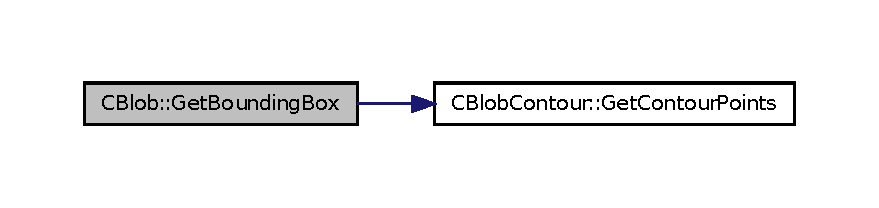
\includegraphics[width=400pt]{class_c_blob_a5391167c172eb461eb762fbdd81306de_cgraph}
\end{center}
\end{figure}




Here is the caller graph for this function:
\nopagebreak
\begin{figure}[H]
\begin{center}
\leavevmode
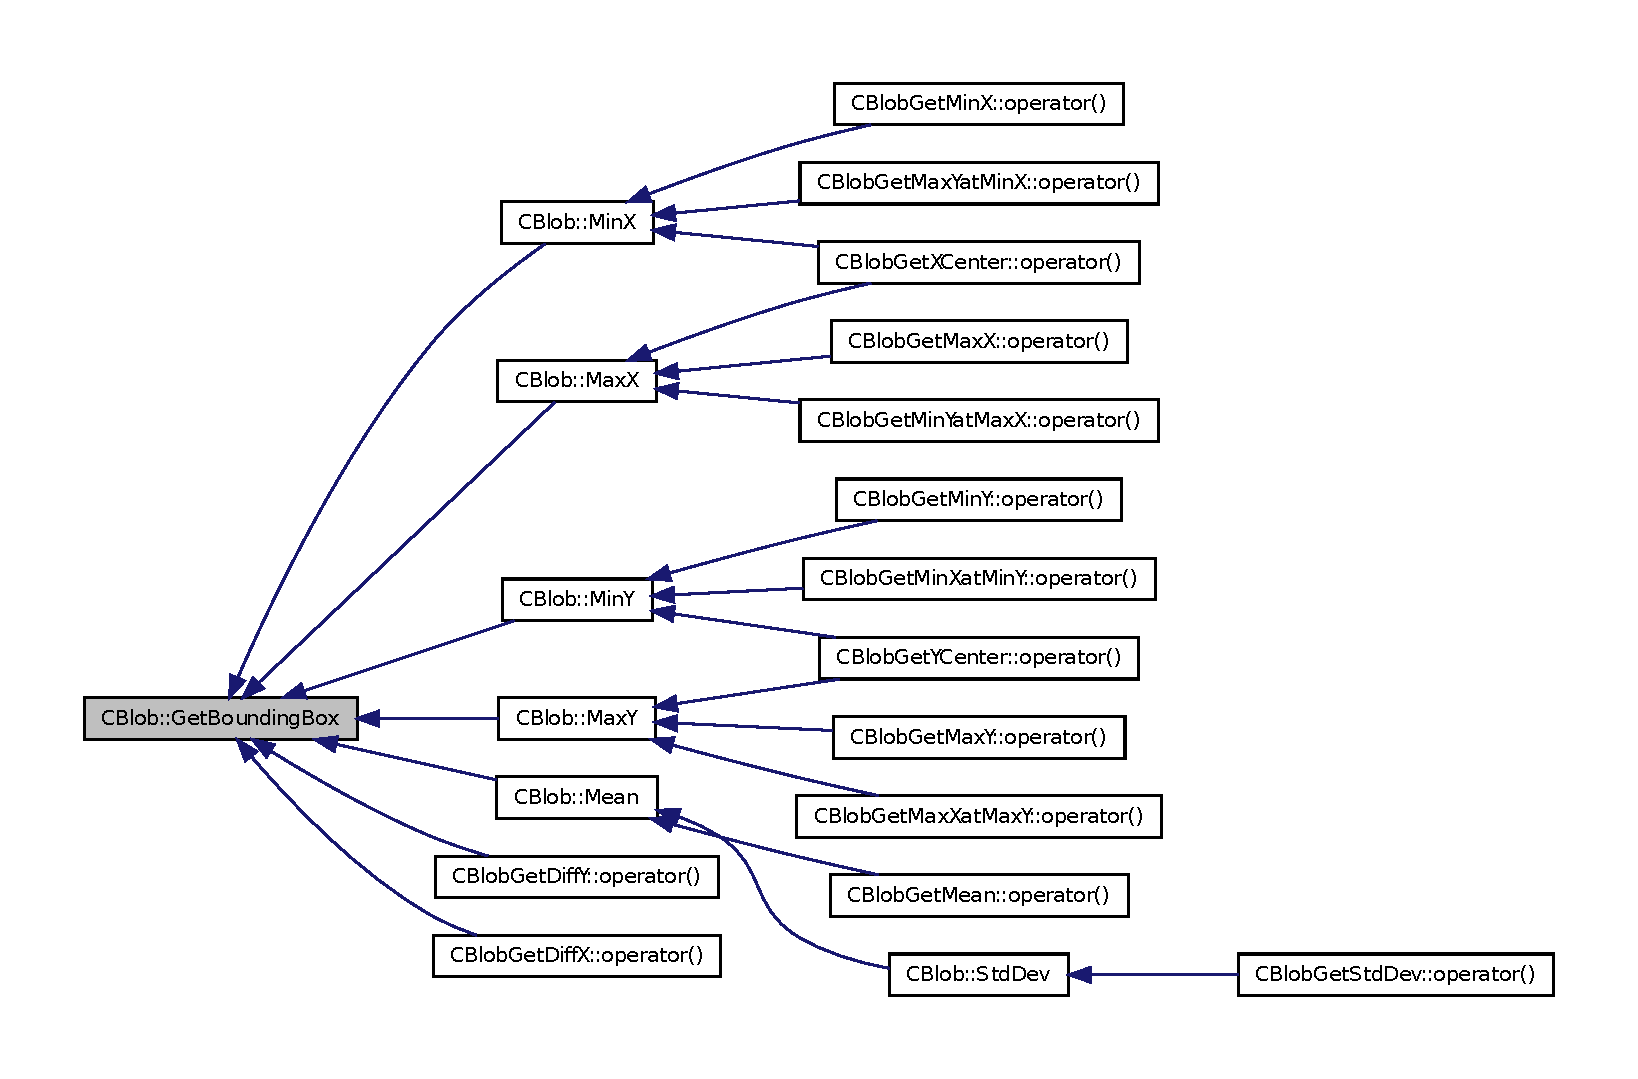
\includegraphics[width=400pt]{class_c_blob_a5391167c172eb461eb762fbdd81306de_icgraph}
\end{center}
\end{figure}


\hypertarget{class_c_blob_aacc50d5d47e0543d4e0a569d05009006}{
\index{CBlob@{CBlob}!GetConvexHull@{GetConvexHull}}
\index{GetConvexHull@{GetConvexHull}!CBlob@{CBlob}}
\subsubsection[{GetConvexHull}]{\setlength{\rightskip}{0pt plus 5cm}{\bf t\_\-PointList} CBlob::GetConvexHull (
\begin{DoxyParamCaption}
{}
\end{DoxyParamCaption}
)}}
\label{class_c_blob_aacc50d5d47e0543d4e0a569d05009006}
Retorna el poligon convex del blob Calculates the convex hull of the blob


\begin{DoxyItemize}
\item FUNCTION: GetConvexHull
\item FUNCTIONALITY: Calculates the convex hull polygon of the blob
\item PARAMETERS:
\begin{DoxyItemize}
\item dst: where to store the result
\end{DoxyItemize}
\item RESULT:
\begin{DoxyItemize}
\item true if no error ocurred
\end{DoxyItemize}
\item RESTRICTIONS:
\item AUTHOR: Ricard Borr�s
\item CREATION DATE: 25-\/05-\/2005.
\item MODIFICATION: Date. Author. Description. 
\end{DoxyItemize}

Here is the call graph for this function:
\nopagebreak
\begin{figure}[H]
\begin{center}
\leavevmode
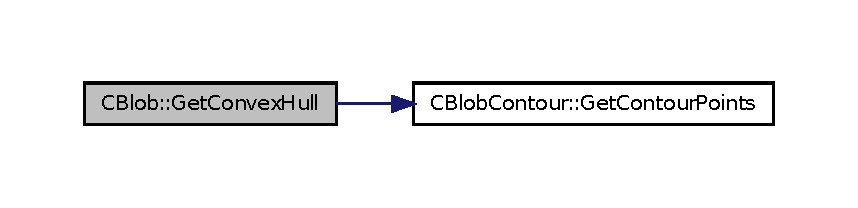
\includegraphics[width=400pt]{class_c_blob_aacc50d5d47e0543d4e0a569d05009006_cgraph}
\end{center}
\end{figure}




Here is the caller graph for this function:
\nopagebreak
\begin{figure}[H]
\begin{center}
\leavevmode
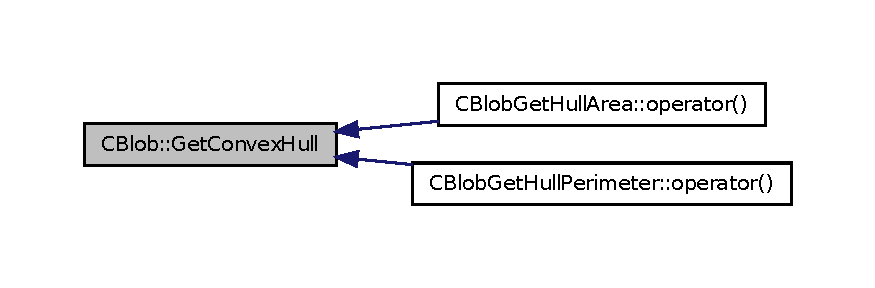
\includegraphics[width=400pt]{class_c_blob_aacc50d5d47e0543d4e0a569d05009006_icgraph}
\end{center}
\end{figure}


\hypertarget{class_c_blob_ad0bb95f395084ee89ca35cf11f203342}{
\index{CBlob@{CBlob}!GetEllipse@{GetEllipse}}
\index{GetEllipse@{GetEllipse}!CBlob@{CBlob}}
\subsubsection[{GetEllipse}]{\setlength{\rightskip}{0pt plus 5cm}CvBox2D CBlob::GetEllipse (
\begin{DoxyParamCaption}
{}
\end{DoxyParamCaption}
)}}
\label{class_c_blob_ad0bb95f395084ee89ca35cf11f203342}


Get bounding ellipse. 


\begin{DoxyItemize}
\item FUNCI�: GetEllipse
\item FUNCIONALITAT: Calculates bounding ellipse of external contour points
\item PAR�METRES:
\begin{DoxyItemize}
\item 
\end{DoxyItemize}
\item RESULTAT:
\begin{DoxyItemize}
\item 
\end{DoxyItemize}
\item RESTRICCIONS:
\begin{DoxyItemize}
\item 
\end{DoxyItemize}
\item AUTOR: rborras
\item DATA DE CREACI�: 2008/05/06
\item MODIFICACI�: Data. Autor. Descripci�.
\item NOTA: Calculation is made using second order moment aproximation 
\end{DoxyItemize}

Here is the call graph for this function:
\nopagebreak
\begin{figure}[H]
\begin{center}
\leavevmode
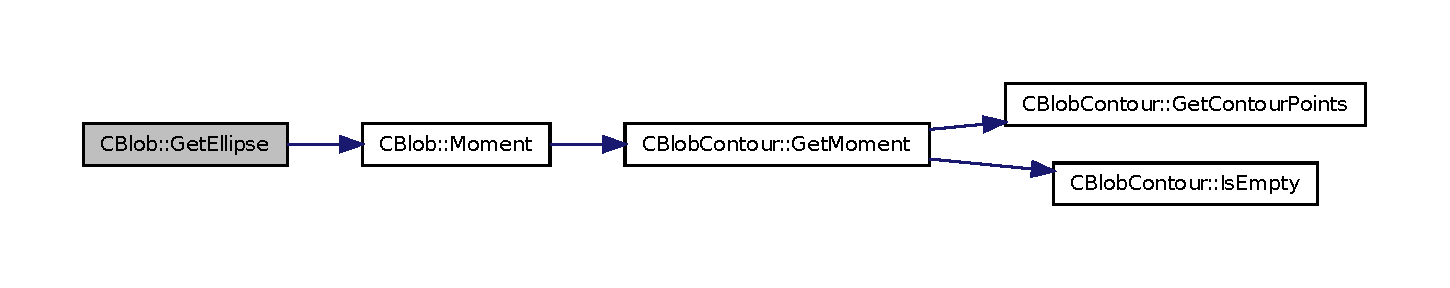
\includegraphics[width=400pt]{class_c_blob_ad0bb95f395084ee89ca35cf11f203342_cgraph}
\end{center}
\end{figure}




Here is the caller graph for this function:
\nopagebreak
\begin{figure}[H]
\begin{center}
\leavevmode
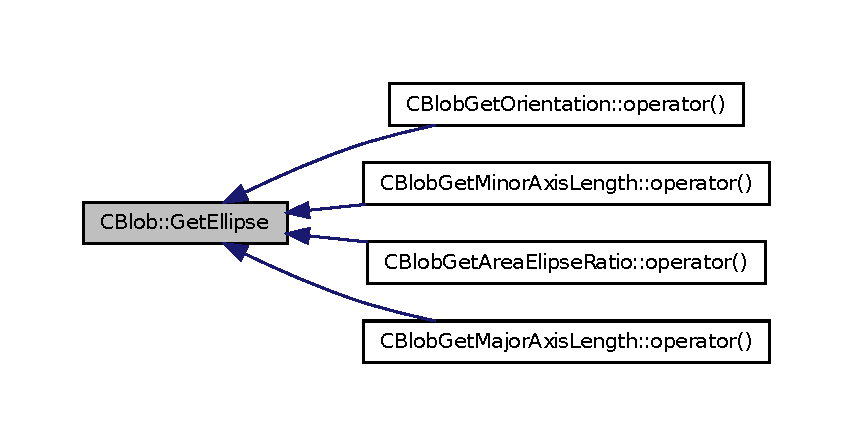
\includegraphics[width=400pt]{class_c_blob_ad0bb95f395084ee89ca35cf11f203342_icgraph}
\end{center}
\end{figure}


\hypertarget{class_c_blob_ad136387165bd74c368cb4ecc7632e4cf}{
\index{CBlob@{CBlob}!GetExternalContour@{GetExternalContour}}
\index{GetExternalContour@{GetExternalContour}!CBlob@{CBlob}}
\subsubsection[{GetExternalContour}]{\setlength{\rightskip}{0pt plus 5cm}{\bf CBlobContour}$\ast$ CBlob::GetExternalContour (
\begin{DoxyParamCaption}
{}
\end{DoxyParamCaption}
)\hspace{0.3cm}{\ttfamily  \mbox{[}inline\mbox{]}}}}
\label{class_c_blob_ad136387165bd74c368cb4ecc7632e4cf}


Retrieves contour in Freeman's chain code. 



Here is the caller graph for this function:
\nopagebreak
\begin{figure}[H]
\begin{center}
\leavevmode
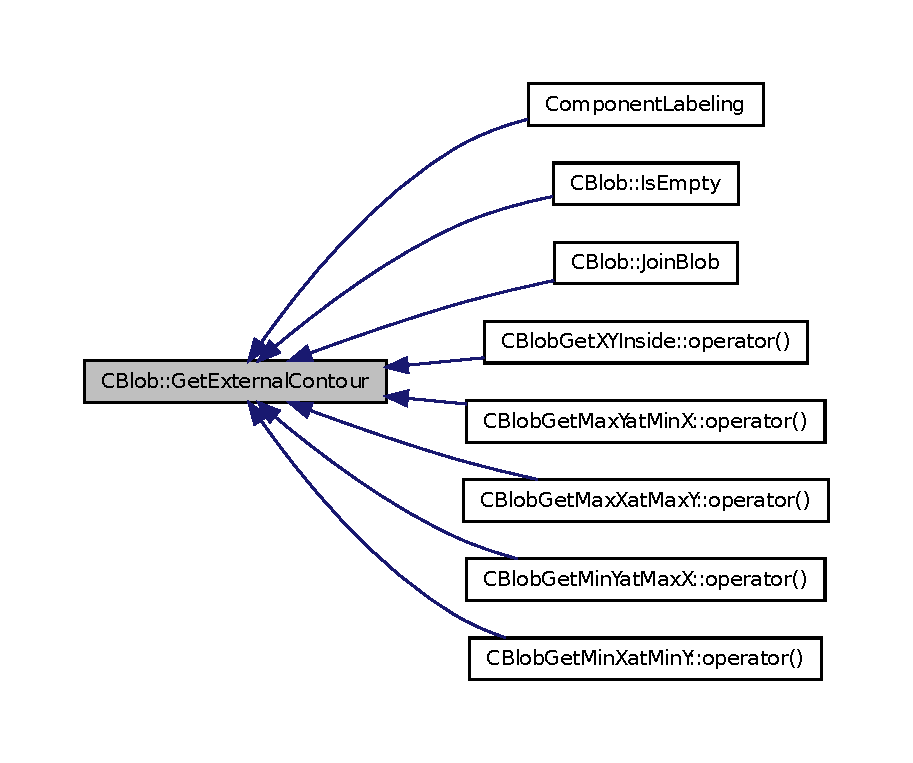
\includegraphics[width=400pt]{class_c_blob_ad136387165bd74c368cb4ecc7632e4cf_icgraph}
\end{center}
\end{figure}


\hypertarget{class_c_blob_a1d3fd90bc98f6d845babb18a3f058bc2}{
\index{CBlob@{CBlob}!GetID@{GetID}}
\index{GetID@{GetID}!CBlob@{CBlob}}
\subsubsection[{GetID}]{\setlength{\rightskip}{0pt plus 5cm}{\bf t\_\-labelType} CBlob::GetID (
\begin{DoxyParamCaption}
{}
\end{DoxyParamCaption}
)\hspace{0.3cm}{\ttfamily  \mbox{[}inline\mbox{]}}}}
\label{class_c_blob_a1d3fd90bc98f6d845babb18a3f058bc2}


Get label ID. 



Here is the caller graph for this function:
\nopagebreak
\begin{figure}[H]
\begin{center}
\leavevmode
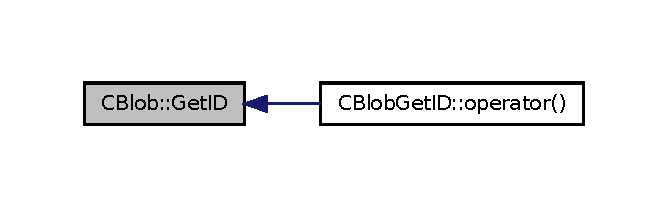
\includegraphics[width=320pt]{class_c_blob_a1d3fd90bc98f6d845babb18a3f058bc2_icgraph}
\end{center}
\end{figure}


\hypertarget{class_c_blob_a1eeee72a4369dc9485c6ae6573631a02}{
\index{CBlob@{CBlob}!GetStorage@{GetStorage}}
\index{GetStorage@{GetStorage}!CBlob@{CBlob}}
\subsubsection[{GetStorage}]{\setlength{\rightskip}{0pt plus 5cm}CvMemStorage$\ast$ CBlob::GetStorage (
\begin{DoxyParamCaption}
{}
\end{DoxyParamCaption}
)\hspace{0.3cm}{\ttfamily  \mbox{[}inline\mbox{]}}}}
\label{class_c_blob_a1eeee72a4369dc9485c6ae6573631a02}


Retrieves blob storage. 



Here is the caller graph for this function:
\nopagebreak
\begin{figure}[H]
\begin{center}
\leavevmode
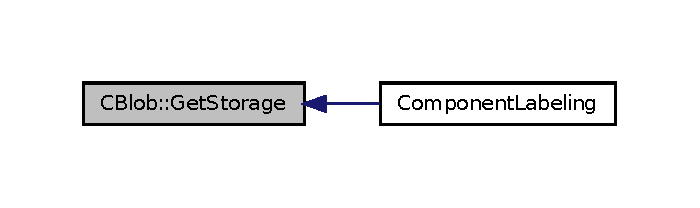
\includegraphics[width=336pt]{class_c_blob_a1eeee72a4369dc9485c6ae6573631a02_icgraph}
\end{center}
\end{figure}


\hypertarget{class_c_blob_ac97e73d3040530de09a187d02632deb1}{
\index{CBlob@{CBlob}!IsEmpty@{IsEmpty}}
\index{IsEmpty@{IsEmpty}!CBlob@{CBlob}}
\subsubsection[{IsEmpty}]{\setlength{\rightskip}{0pt plus 5cm}bool CBlob::IsEmpty (
\begin{DoxyParamCaption}
{}
\end{DoxyParamCaption}
)}}
\label{class_c_blob_ac97e73d3040530de09a187d02632deb1}
Indica si el blob est� buit ( no t� cap info associada ) Shows if the blob has associated information 

Here is the call graph for this function:
\nopagebreak
\begin{figure}[H]
\begin{center}
\leavevmode
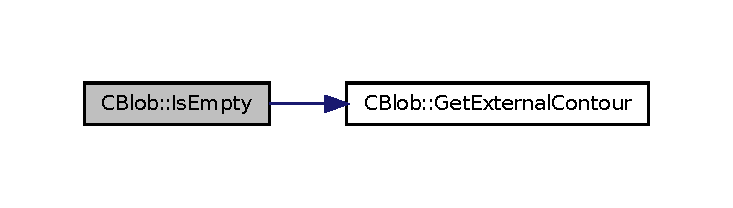
\includegraphics[width=352pt]{class_c_blob_ac97e73d3040530de09a187d02632deb1_cgraph}
\end{center}
\end{figure}


\hypertarget{class_c_blob_a006463cc42ef0e4b8986fa5020cb6f90}{
\index{CBlob@{CBlob}!JoinBlob@{JoinBlob}}
\index{JoinBlob@{JoinBlob}!CBlob@{CBlob}}
\subsubsection[{JoinBlob}]{\setlength{\rightskip}{0pt plus 5cm}void CBlob::JoinBlob (
\begin{DoxyParamCaption}
\item[{{\bf CBlob} $\ast$}]{ blob}
\end{DoxyParamCaption}
)}}
\label{class_c_blob_a006463cc42ef0e4b8986fa5020cb6f90}


Join a blob to current one (add's contour. 


\begin{DoxyItemize}
\item FUNCTION: JoinBlob
\item FUNCTIONALITY: Add's external contour to current external contour
\item PARAMETERS:
\begin{DoxyItemize}
\item blob: blob from which extract the added external contour
\end{DoxyItemize}
\item RESULT:
\begin{DoxyItemize}
\item true if no error ocurred
\end{DoxyItemize}
\item RESTRICTIONS: Only external contours are added
\item AUTHOR: Ricard Borr�s
\item CREATION DATE: 25-\/05-\/2005.
\item MODIFICATION: Date. Author. Description. 
\end{DoxyItemize}

Here is the call graph for this function:
\nopagebreak
\begin{figure}[H]
\begin{center}
\leavevmode
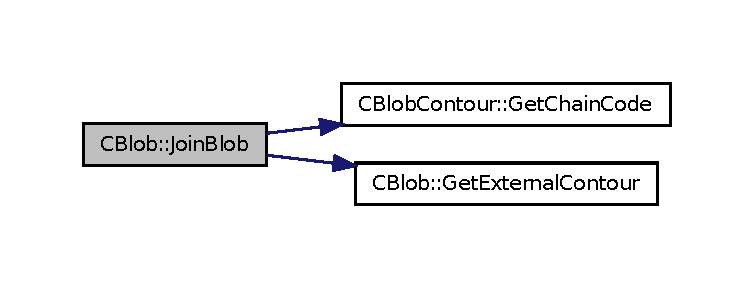
\includegraphics[width=362pt]{class_c_blob_a006463cc42ef0e4b8986fa5020cb6f90_cgraph}
\end{center}
\end{figure}


\hypertarget{class_c_blob_ab26a757fffc581df39620425de008cbc}{
\index{CBlob@{CBlob}!MaxX@{MaxX}}
\index{MaxX@{MaxX}!CBlob@{CBlob}}
\subsubsection[{MaxX}]{\setlength{\rightskip}{0pt plus 5cm}double CBlob::MaxX (
\begin{DoxyParamCaption}
{}
\end{DoxyParamCaption}
)\hspace{0.3cm}{\ttfamily  \mbox{[}inline\mbox{]}}}}
\label{class_c_blob_ab26a757fffc581df39620425de008cbc}


Maximun X. 



Here is the call graph for this function:
\nopagebreak
\begin{figure}[H]
\begin{center}
\leavevmode
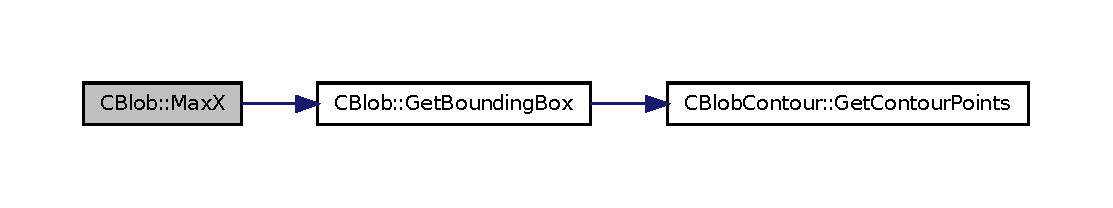
\includegraphics[width=400pt]{class_c_blob_ab26a757fffc581df39620425de008cbc_cgraph}
\end{center}
\end{figure}




Here is the caller graph for this function:
\nopagebreak
\begin{figure}[H]
\begin{center}
\leavevmode
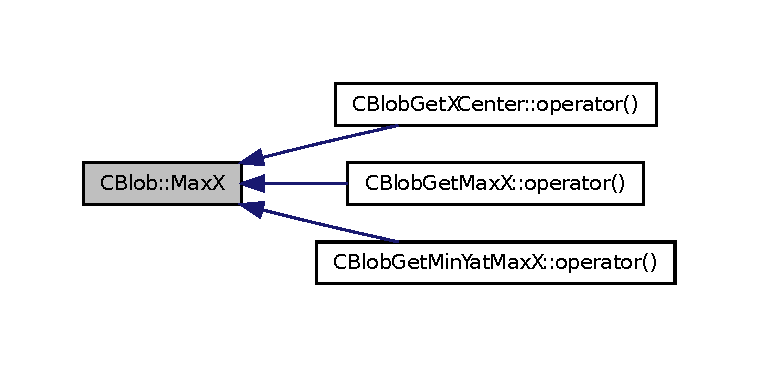
\includegraphics[width=364pt]{class_c_blob_ab26a757fffc581df39620425de008cbc_icgraph}
\end{center}
\end{figure}


\hypertarget{class_c_blob_a740a37afcd841bf719587d2f0128c555}{
\index{CBlob@{CBlob}!MaxY@{MaxY}}
\index{MaxY@{MaxY}!CBlob@{CBlob}}
\subsubsection[{MaxY}]{\setlength{\rightskip}{0pt plus 5cm}double CBlob::MaxY (
\begin{DoxyParamCaption}
{}
\end{DoxyParamCaption}
)\hspace{0.3cm}{\ttfamily  \mbox{[}inline\mbox{]}}}}
\label{class_c_blob_a740a37afcd841bf719587d2f0128c555}


Maximun Y. 



Here is the call graph for this function:
\nopagebreak
\begin{figure}[H]
\begin{center}
\leavevmode
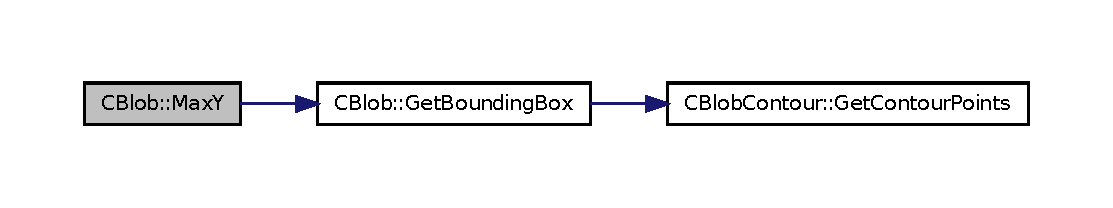
\includegraphics[width=400pt]{class_c_blob_a740a37afcd841bf719587d2f0128c555_cgraph}
\end{center}
\end{figure}




Here is the caller graph for this function:
\nopagebreak
\begin{figure}[H]
\begin{center}
\leavevmode
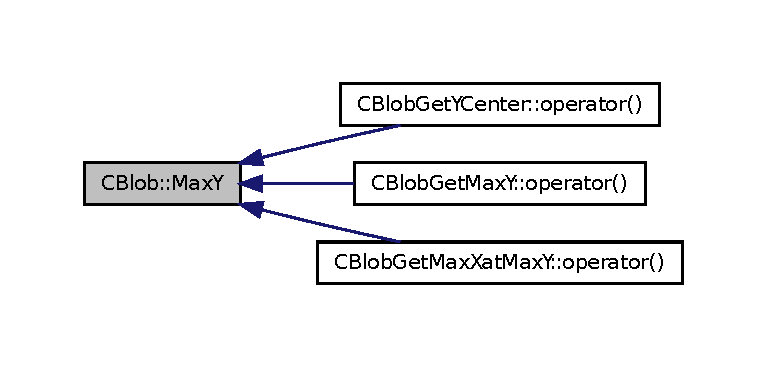
\includegraphics[width=368pt]{class_c_blob_a740a37afcd841bf719587d2f0128c555_icgraph}
\end{center}
\end{figure}


\hypertarget{class_c_blob_a1b12d25f8e470fdd808ac2e3bfe9bad4}{
\index{CBlob@{CBlob}!Mean@{Mean}}
\index{Mean@{Mean}!CBlob@{CBlob}}
\subsubsection[{Mean}]{\setlength{\rightskip}{0pt plus 5cm}double CBlob::Mean (
\begin{DoxyParamCaption}
\item[{IplImage $\ast$}]{ image}
\end{DoxyParamCaption}
)}}
\label{class_c_blob_a1b12d25f8e470fdd808ac2e3bfe9bad4}


Get mean grey color. 


\begin{DoxyItemize}
\item FUNCI�: Mean
\item FUNCIONALITAT: Get blob mean color in input image
\item PAR�METRES:
\begin{DoxyItemize}
\item image: image from gray color are extracted
\end{DoxyItemize}
\item RESULTAT:
\begin{DoxyItemize}
\item 
\end{DoxyItemize}
\item RESTRICCIONS:
\begin{DoxyItemize}
\item 
\end{DoxyItemize}
\item AUTOR: rborras
\item DATA DE CREACI�: 2008/05/06
\item MODIFICACI�: Data. Autor. Descripci�. 
\end{DoxyItemize}

Here is the call graph for this function:
\nopagebreak
\begin{figure}[H]
\begin{center}
\leavevmode
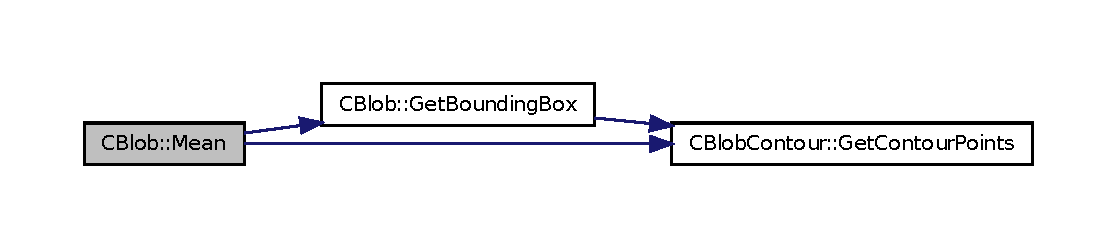
\includegraphics[width=400pt]{class_c_blob_a1b12d25f8e470fdd808ac2e3bfe9bad4_cgraph}
\end{center}
\end{figure}




Here is the caller graph for this function:
\nopagebreak
\begin{figure}[H]
\begin{center}
\leavevmode
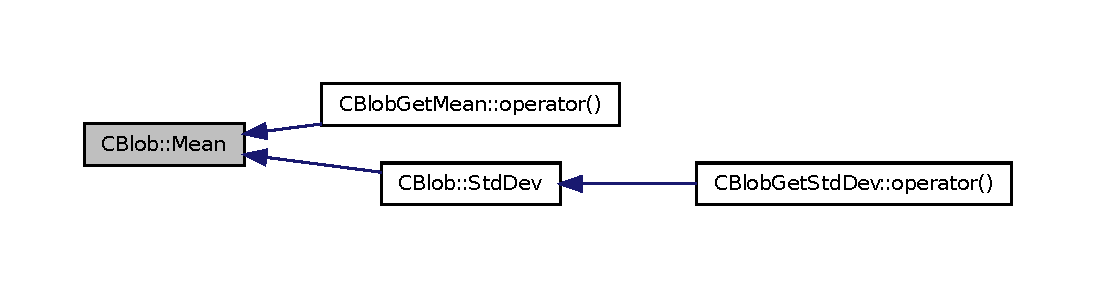
\includegraphics[width=400pt]{class_c_blob_a1b12d25f8e470fdd808ac2e3bfe9bad4_icgraph}
\end{center}
\end{figure}


\hypertarget{class_c_blob_aa3313af22e7f28d65ba245bc3b8a30bc}{
\index{CBlob@{CBlob}!MinX@{MinX}}
\index{MinX@{MinX}!CBlob@{CBlob}}
\subsubsection[{MinX}]{\setlength{\rightskip}{0pt plus 5cm}double CBlob::MinX (
\begin{DoxyParamCaption}
{}
\end{DoxyParamCaption}
)\hspace{0.3cm}{\ttfamily  \mbox{[}inline\mbox{]}}}}
\label{class_c_blob_aa3313af22e7f28d65ba245bc3b8a30bc}


Minimun X. 



Here is the call graph for this function:
\nopagebreak
\begin{figure}[H]
\begin{center}
\leavevmode
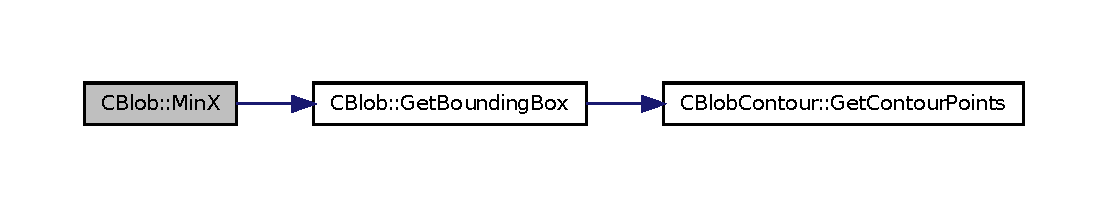
\includegraphics[width=400pt]{class_c_blob_aa3313af22e7f28d65ba245bc3b8a30bc_cgraph}
\end{center}
\end{figure}




Here is the caller graph for this function:
\nopagebreak
\begin{figure}[H]
\begin{center}
\leavevmode
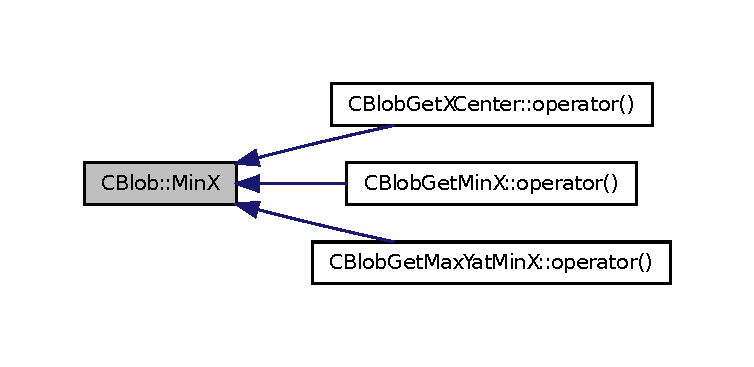
\includegraphics[width=362pt]{class_c_blob_aa3313af22e7f28d65ba245bc3b8a30bc_icgraph}
\end{center}
\end{figure}


\hypertarget{class_c_blob_a44e2caf6c7fc6e8360d2576c18c9bc2b}{
\index{CBlob@{CBlob}!MinY@{MinY}}
\index{MinY@{MinY}!CBlob@{CBlob}}
\subsubsection[{MinY}]{\setlength{\rightskip}{0pt plus 5cm}double CBlob::MinY (
\begin{DoxyParamCaption}
{}
\end{DoxyParamCaption}
)\hspace{0.3cm}{\ttfamily  \mbox{[}inline\mbox{]}}}}
\label{class_c_blob_a44e2caf6c7fc6e8360d2576c18c9bc2b}


Minimun Y. 



Here is the call graph for this function:
\nopagebreak
\begin{figure}[H]
\begin{center}
\leavevmode
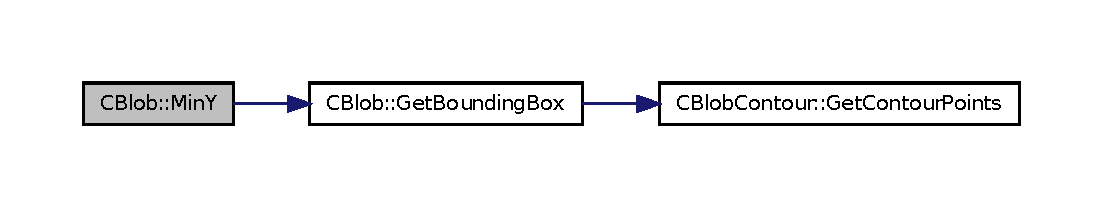
\includegraphics[width=400pt]{class_c_blob_a44e2caf6c7fc6e8360d2576c18c9bc2b_cgraph}
\end{center}
\end{figure}




Here is the caller graph for this function:
\nopagebreak
\begin{figure}[H]
\begin{center}
\leavevmode
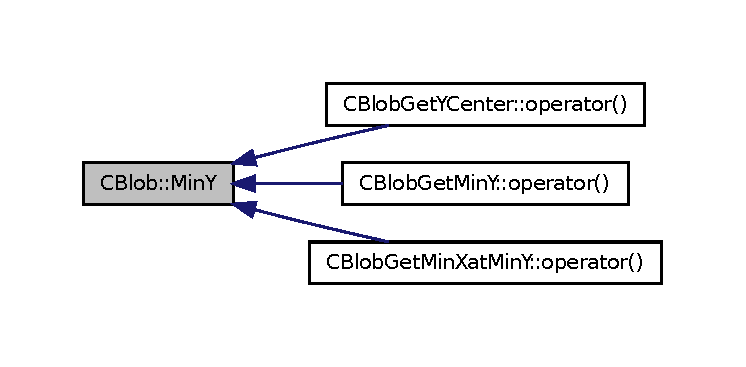
\includegraphics[width=358pt]{class_c_blob_a44e2caf6c7fc6e8360d2576c18c9bc2b_icgraph}
\end{center}
\end{figure}


\hypertarget{class_c_blob_a4f5dfca1ee933e07a39965375f9f07c5}{
\index{CBlob@{CBlob}!Moment@{Moment}}
\index{Moment@{Moment}!CBlob@{CBlob}}
\subsubsection[{Moment}]{\setlength{\rightskip}{0pt plus 5cm}double CBlob::Moment (
\begin{DoxyParamCaption}
\item[{int}]{ p, }
\item[{int}]{ q}
\end{DoxyParamCaption}
)}}
\label{class_c_blob_a4f5dfca1ee933e07a39965375f9f07c5}


Compute blob's moment (p,q up to MAX\_\-CALCULATED\_\-MOMENTS). 



Here is the call graph for this function:
\nopagebreak
\begin{figure}[H]
\begin{center}
\leavevmode
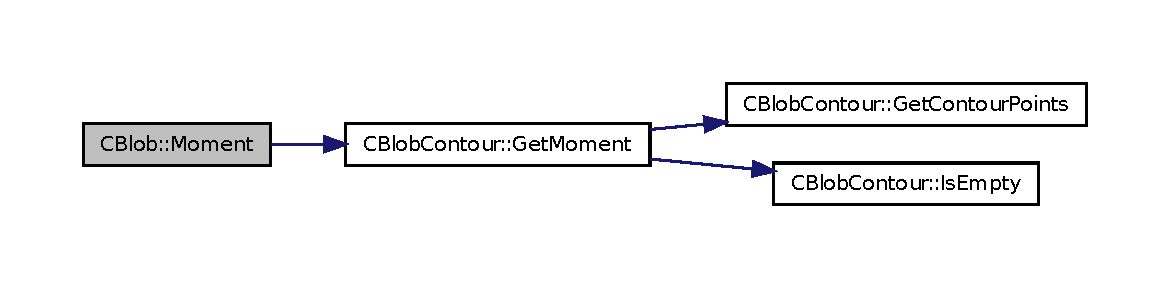
\includegraphics[width=400pt]{class_c_blob_a4f5dfca1ee933e07a39965375f9f07c5_cgraph}
\end{center}
\end{figure}




Here is the caller graph for this function:
\nopagebreak
\begin{figure}[H]
\begin{center}
\leavevmode
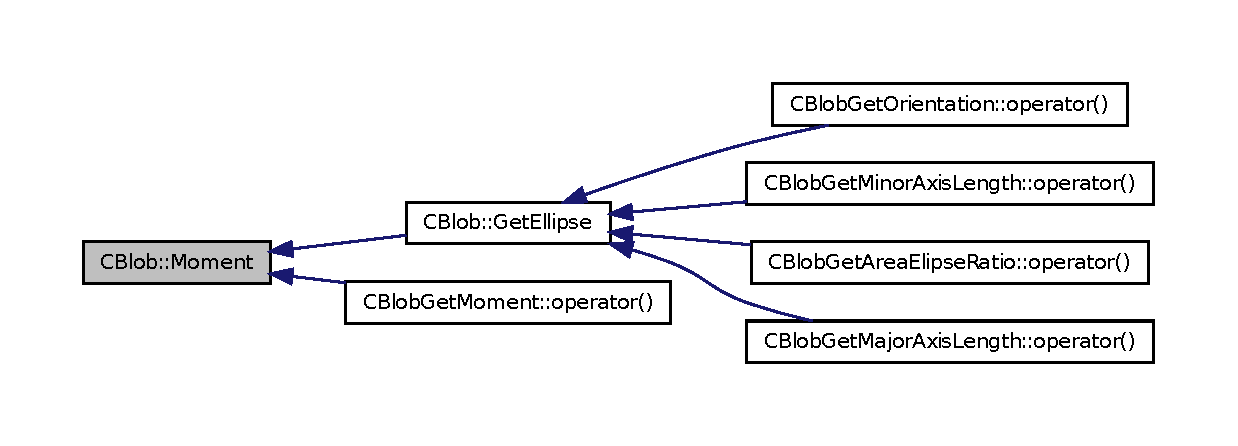
\includegraphics[width=400pt]{class_c_blob_a4f5dfca1ee933e07a39965375f9f07c5_icgraph}
\end{center}
\end{figure}


\hypertarget{class_c_blob_a724e55442a030bf94da856310e324a40}{
\index{CBlob@{CBlob}!operator=@{operator=}}
\index{operator=@{operator=}!CBlob@{CBlob}}
\subsubsection[{operator=}]{\setlength{\rightskip}{0pt plus 5cm}{\bf CBlob} \& CBlob::operator= (
\begin{DoxyParamCaption}
\item[{const {\bf CBlob} \&}]{ src}
\end{DoxyParamCaption}
)}}
\label{class_c_blob_a724e55442a030bf94da856310e324a40}
Operador d'assignaci� Assigment operator 

Here is the call graph for this function:
\nopagebreak
\begin{figure}[H]
\begin{center}
\leavevmode
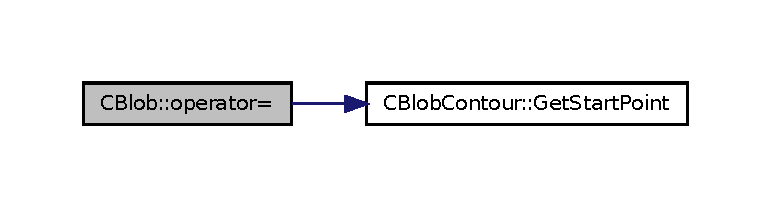
\includegraphics[width=370pt]{class_c_blob_a724e55442a030bf94da856310e324a40_cgraph}
\end{center}
\end{figure}


\hypertarget{class_c_blob_af63853ea55dbebbee5b013189e765b51}{
\index{CBlob@{CBlob}!Perimeter@{Perimeter}}
\index{Perimeter@{Perimeter}!CBlob@{CBlob}}
\subsubsection[{Perimeter}]{\setlength{\rightskip}{0pt plus 5cm}double CBlob::Perimeter (
\begin{DoxyParamCaption}
{}
\end{DoxyParamCaption}
)}}
\label{class_c_blob_af63853ea55dbebbee5b013189e765b51}


Compute blob's perimeter. 


\begin{DoxyItemize}
\item FUNCI�: Perimeter
\item FUNCIONALITAT: Get blob perimeter, ie. sum of the lenght of all the contours
\item PAR�METRES:
\begin{DoxyItemize}
\item 
\end{DoxyItemize}
\item RESULTAT:
\begin{DoxyItemize}
\item 
\end{DoxyItemize}
\item RESTRICCIONS:
\begin{DoxyItemize}
\item 
\end{DoxyItemize}
\item AUTOR: rborras
\item DATA DE CREACI�: 2008/04/30
\item MODIFICACI�: Data. Autor. Descripci�. 
\end{DoxyItemize}

Here is the call graph for this function:
\nopagebreak
\begin{figure}[H]
\begin{center}
\leavevmode
\includegraphics[width=400pt]{class_c_blob_af63853ea55dbebbee5b013189e765b51_cgraph}
\end{center}
\end{figure}




Here is the caller graph for this function:
\nopagebreak
\begin{figure}[H]
\begin{center}
\leavevmode
\includegraphics[width=400pt]{class_c_blob_af63853ea55dbebbee5b013189e765b51_icgraph}
\end{center}
\end{figure}


\hypertarget{class_c_blob_a014b670bb748e6767ef070e1bc25be7a}{
\index{CBlob@{CBlob}!StdDev@{StdDev}}
\index{StdDev@{StdDev}!CBlob@{CBlob}}
\subsubsection[{StdDev}]{\setlength{\rightskip}{0pt plus 5cm}double CBlob::StdDev (
\begin{DoxyParamCaption}
\item[{IplImage $\ast$}]{ image}
\end{DoxyParamCaption}
)}}
\label{class_c_blob_a014b670bb748e6767ef070e1bc25be7a}


Get standard deviation grey color. 



Here is the call graph for this function:
\nopagebreak
\begin{figure}[H]
\begin{center}
\leavevmode
\includegraphics[width=400pt]{class_c_blob_a014b670bb748e6767ef070e1bc25be7a_cgraph}
\end{center}
\end{figure}




Here is the caller graph for this function:
\nopagebreak
\begin{figure}[H]
\begin{center}
\leavevmode
\includegraphics[width=354pt]{class_c_blob_a014b670bb748e6767ef070e1bc25be7a_icgraph}
\end{center}
\end{figure}




The documentation for this class was generated from the following files:\begin{DoxyCompactItemize}
\item 
src/3rdparty/cvblobs/\hyperlink{blob_8h}{blob.h}\item 
src/3rdparty/cvblobs/\hyperlink{blob_8cpp}{blob.cpp}\end{DoxyCompactItemize}

\hypertarget{class_c_blob_contour}{
\section{CBlobContour Class Reference}
\label{class_c_blob_contour}\index{CBlobContour@{CBlobContour}}
}


Blob contour class (in crack code).  




{\ttfamily \#include $<$BlobContour.h$>$}

\subsection*{Public Member Functions}
\begin{DoxyCompactItemize}
\item 
\hyperlink{class_c_blob_contour_a4cfb475c4e55945fe13618768bef57c7}{CBlobContour} ()
\begin{DoxyCompactList}\small\item\em Constructors. \item\end{DoxyCompactList}\item 
\hyperlink{class_c_blob_contour_a66a78de7519f1e8ae7b92bdc30a726cc}{CBlobContour} (CvPoint startPoint, CvMemStorage $\ast$storage)
\item 
\hyperlink{class_c_blob_contour_a24b82910c8cfb9b0a31a3fb55fd29e28}{CBlobContour} (\hyperlink{class_c_blob_contour}{CBlobContour} $\ast$source)
\begin{DoxyCompactList}\small\item\em Copy constructor. \item\end{DoxyCompactList}\item 
\hyperlink{class_c_blob_contour_a24c825e7c0fab7e98237a2db60a7fc7a}{$\sim$CBlobContour} ()
\item 
\hyperlink{class_c_blob_contour}{CBlobContour} \& \hyperlink{class_c_blob_contour_a9ed6e0471a8d1b7d6c9a1465e539bbd4}{operator=} (const \hyperlink{class_c_blob_contour}{CBlobContour} \&source)
\begin{DoxyCompactList}\small\item\em Assigment operator. \item\end{DoxyCompactList}\item 
void \hyperlink{class_c_blob_contour_a5a10813d71e48c52e099001e6581366c}{AddChainCode} (\hyperlink{_blob_contour_8h_a0ccb8765a7971147eaf6cafef4bd3c0e}{t\_\-chainCode} code)
\begin{DoxyCompactList}\small\item\em Add chain code to contour. \item\end{DoxyCompactList}\item 
\hyperlink{_blob_contour_8h_af4605a71deb8fb5bf67011c89418c970}{t\_\-chainCodeList} \hyperlink{class_c_blob_contour_ae783c063f2d89f4d06396b552c92f9a6}{GetChainCode} ()
\begin{DoxyCompactList}\small\item\em Return freeman chain coded contour. \item\end{DoxyCompactList}\item 
bool \hyperlink{class_c_blob_contour_af4e715a94924d5dc1a0e67cf75818bb5}{IsEmpty} ()
\item 
\hyperlink{_blob_contour_8h_af4605a71deb8fb5bf67011c89418c970}{t\_\-chainCodeList} \hyperlink{class_c_blob_contour_a245d5e59180619aa9ae4ec14acc18744}{GetContourPoints} ()
\begin{DoxyCompactList}\small\item\em Return all contour points. \item\end{DoxyCompactList}\end{DoxyCompactItemize}
\subsection*{Protected Member Functions}
\begin{DoxyCompactItemize}
\item 
CvPoint \hyperlink{class_c_blob_contour_ac8f0fbdce452ede583013e010ce0c8e3}{GetStartPoint} () const 
\item 
void \hyperlink{class_c_blob_contour_a9a9ea170c2100586ca7bdb4227589fe9}{ResetChainCode} ()
\begin{DoxyCompactList}\small\item\em Clears chain code contour. \item\end{DoxyCompactList}\item 
double \hyperlink{class_c_blob_contour_a2c68f462fc31a0e7add9a85b007fa42a}{GetArea} ()
\begin{DoxyCompactList}\small\item\em Computes area from contour. \item\end{DoxyCompactList}\item 
double \hyperlink{class_c_blob_contour_a893d57d625bb8f26f4a31ff0b66b8406}{GetPerimeter} ()
\begin{DoxyCompactList}\small\item\em Computes perimeter from contour. \item\end{DoxyCompactList}\item 
double \hyperlink{class_c_blob_contour_a301727633680b38714302593945b748f}{GetMoment} (int p, int q)
\begin{DoxyCompactList}\small\item\em Get contour moment (p,q up to MAX\_\-CALCULATED\_\-MOMENTS). \item\end{DoxyCompactList}\end{DoxyCompactItemize}
\subsection*{Protected Attributes}
\begin{DoxyCompactItemize}
\item 
\hyperlink{_blob_contour_8h_af4605a71deb8fb5bf67011c89418c970}{t\_\-chainCodeList} \hyperlink{class_c_blob_contour_a98c36d7be8524da3976fad97b611123e}{m\_\-contour}
\begin{DoxyCompactList}\small\item\em Crack code list. \item\end{DoxyCompactList}\end{DoxyCompactItemize}
\subsection*{Friends}
\begin{DoxyCompactItemize}
\item 
class \hyperlink{class_c_blob_contour_ae1a0519c97d58c87882ff9a1462ae464}{CBlob}
\item 
class \hyperlink{class_c_blob_contour_a107dcb6bc234839a49f6a53dde777713}{CBlobProperties}
\end{DoxyCompactItemize}


\subsection{Detailed Description}
Blob contour class (in crack code). 

\subsection{Constructor \& Destructor Documentation}
\hypertarget{class_c_blob_contour_a4cfb475c4e55945fe13618768bef57c7}{
\index{CBlobContour@{CBlobContour}!CBlobContour@{CBlobContour}}
\index{CBlobContour@{CBlobContour}!CBlobContour@{CBlobContour}}
\subsubsection[{CBlobContour}]{\setlength{\rightskip}{0pt plus 5cm}CBlobContour::CBlobContour (
\begin{DoxyParamCaption}
{}
\end{DoxyParamCaption}
)}}
\label{class_c_blob_contour_a4cfb475c4e55945fe13618768bef57c7}


Constructors. 

\hypertarget{class_c_blob_contour_a66a78de7519f1e8ae7b92bdc30a726cc}{
\index{CBlobContour@{CBlobContour}!CBlobContour@{CBlobContour}}
\index{CBlobContour@{CBlobContour}!CBlobContour@{CBlobContour}}
\subsubsection[{CBlobContour}]{\setlength{\rightskip}{0pt plus 5cm}CBlobContour::CBlobContour (
\begin{DoxyParamCaption}
\item[{CvPoint}]{ startPoint, }
\item[{CvMemStorage $\ast$}]{ storage}
\end{DoxyParamCaption}
)}}
\label{class_c_blob_contour_a66a78de7519f1e8ae7b92bdc30a726cc}
\hypertarget{class_c_blob_contour_a24b82910c8cfb9b0a31a3fb55fd29e28}{
\index{CBlobContour@{CBlobContour}!CBlobContour@{CBlobContour}}
\index{CBlobContour@{CBlobContour}!CBlobContour@{CBlobContour}}
\subsubsection[{CBlobContour}]{\setlength{\rightskip}{0pt plus 5cm}CBlobContour::CBlobContour (
\begin{DoxyParamCaption}
\item[{{\bf CBlobContour} $\ast$}]{ source}
\end{DoxyParamCaption}
)}}
\label{class_c_blob_contour_a24b82910c8cfb9b0a31a3fb55fd29e28}


Copy constructor. 

\hypertarget{class_c_blob_contour_a24c825e7c0fab7e98237a2db60a7fc7a}{
\index{CBlobContour@{CBlobContour}!$\sim$CBlobContour@{$\sim$CBlobContour}}
\index{$\sim$CBlobContour@{$\sim$CBlobContour}!CBlobContour@{CBlobContour}}
\subsubsection[{$\sim$CBlobContour}]{\setlength{\rightskip}{0pt plus 5cm}CBlobContour::$\sim$CBlobContour (
\begin{DoxyParamCaption}
{}
\end{DoxyParamCaption}
)}}
\label{class_c_blob_contour_a24c825e7c0fab7e98237a2db60a7fc7a}


\subsection{Member Function Documentation}
\hypertarget{class_c_blob_contour_a5a10813d71e48c52e099001e6581366c}{
\index{CBlobContour@{CBlobContour}!AddChainCode@{AddChainCode}}
\index{AddChainCode@{AddChainCode}!CBlobContour@{CBlobContour}}
\subsubsection[{AddChainCode}]{\setlength{\rightskip}{0pt plus 5cm}void CBlobContour::AddChainCode (
\begin{DoxyParamCaption}
\item[{{\bf t\_\-chainCode}}]{ chaincode}
\end{DoxyParamCaption}
)}}
\label{class_c_blob_contour_a5a10813d71e48c52e099001e6581366c}


Add chain code to contour. 


\begin{DoxyItemize}
\item FUNCI�: AddChainCode
\item FUNCIONALITAT: Add chain code to contour
\item PAR�METRES:
\begin{DoxyItemize}
\item 
\end{DoxyItemize}
\item RESULTAT:
\begin{DoxyItemize}
\item 
\end{DoxyItemize}
\item RESTRICCIONS:
\begin{DoxyItemize}
\item 
\end{DoxyItemize}
\item AUTOR: rborras
\item DATA DE CREACI�: 2008/05/06
\item MODIFICACI�: Data. Autor. Descripci�. 
\end{DoxyItemize}

Here is the caller graph for this function:
\nopagebreak
\begin{figure}[H]
\begin{center}
\leavevmode
\includegraphics[width=400pt]{class_c_blob_contour_a5a10813d71e48c52e099001e6581366c_icgraph}
\end{center}
\end{figure}


\hypertarget{class_c_blob_contour_a2c68f462fc31a0e7add9a85b007fa42a}{
\index{CBlobContour@{CBlobContour}!GetArea@{GetArea}}
\index{GetArea@{GetArea}!CBlobContour@{CBlobContour}}
\subsubsection[{GetArea}]{\setlength{\rightskip}{0pt plus 5cm}double CBlobContour::GetArea (
\begin{DoxyParamCaption}
{}
\end{DoxyParamCaption}
)\hspace{0.3cm}{\ttfamily  \mbox{[}protected\mbox{]}}}}
\label{class_c_blob_contour_a2c68f462fc31a0e7add9a85b007fa42a}


Computes area from contour. 


\begin{DoxyItemize}
\item FUNCI�: GetArea
\item FUNCIONALITAT: Computes area from chain code
\item PAR�METRES:
\begin{DoxyItemize}
\item 
\end{DoxyItemize}
\item RESULTAT:
\begin{DoxyItemize}
\item May give negative areas for clock wise contours
\end{DoxyItemize}
\item RESTRICCIONS:
\begin{DoxyItemize}
\item 
\end{DoxyItemize}
\item AUTOR: rborras
\item DATA DE CREACI�: 2008/04/30
\item MODIFICACI�: Data. Autor. Descripci�.
\item NOTA: Algorithm derived from \char`\"{}Properties of contour codes\char`\"{}, G.R. Wilson 
\end{DoxyItemize}

Here is the call graph for this function:
\nopagebreak
\begin{figure}[H]
\begin{center}
\leavevmode
\includegraphics[width=400pt]{class_c_blob_contour_a2c68f462fc31a0e7add9a85b007fa42a_cgraph}
\end{center}
\end{figure}




Here is the caller graph for this function:
\nopagebreak
\begin{figure}[H]
\begin{center}
\leavevmode
\includegraphics[width=400pt]{class_c_blob_contour_a2c68f462fc31a0e7add9a85b007fa42a_icgraph}
\end{center}
\end{figure}


\hypertarget{class_c_blob_contour_ae783c063f2d89f4d06396b552c92f9a6}{
\index{CBlobContour@{CBlobContour}!GetChainCode@{GetChainCode}}
\index{GetChainCode@{GetChainCode}!CBlobContour@{CBlobContour}}
\subsubsection[{GetChainCode}]{\setlength{\rightskip}{0pt plus 5cm}{\bf t\_\-chainCodeList} CBlobContour::GetChainCode (
\begin{DoxyParamCaption}
{}
\end{DoxyParamCaption}
)\hspace{0.3cm}{\ttfamily  \mbox{[}inline\mbox{]}}}}
\label{class_c_blob_contour_ae783c063f2d89f4d06396b552c92f9a6}


Return freeman chain coded contour. 



Here is the caller graph for this function:
\nopagebreak
\begin{figure}[H]
\begin{center}
\leavevmode
\includegraphics[width=362pt]{class_c_blob_contour_ae783c063f2d89f4d06396b552c92f9a6_icgraph}
\end{center}
\end{figure}


\hypertarget{class_c_blob_contour_a245d5e59180619aa9ae4ec14acc18744}{
\index{CBlobContour@{CBlobContour}!GetContourPoints@{GetContourPoints}}
\index{GetContourPoints@{GetContourPoints}!CBlobContour@{CBlobContour}}
\subsubsection[{GetContourPoints}]{\setlength{\rightskip}{0pt plus 5cm}{\bf t\_\-PointList} CBlobContour::GetContourPoints (
\begin{DoxyParamCaption}
{}
\end{DoxyParamCaption}
)}}
\label{class_c_blob_contour_a245d5e59180619aa9ae4ec14acc18744}


Return all contour points. 

Calculate contour points from crack codes. 

Here is the caller graph for this function:
\nopagebreak
\begin{figure}[H]
\begin{center}
\leavevmode
\includegraphics[width=400pt]{class_c_blob_contour_a245d5e59180619aa9ae4ec14acc18744_icgraph}
\end{center}
\end{figure}


\hypertarget{class_c_blob_contour_a301727633680b38714302593945b748f}{
\index{CBlobContour@{CBlobContour}!GetMoment@{GetMoment}}
\index{GetMoment@{GetMoment}!CBlobContour@{CBlobContour}}
\subsubsection[{GetMoment}]{\setlength{\rightskip}{0pt plus 5cm}double CBlobContour::GetMoment (
\begin{DoxyParamCaption}
\item[{int}]{ p, }
\item[{int}]{ q}
\end{DoxyParamCaption}
)\hspace{0.3cm}{\ttfamily  \mbox{[}protected\mbox{]}}}}
\label{class_c_blob_contour_a301727633680b38714302593945b748f}


Get contour moment (p,q up to MAX\_\-CALCULATED\_\-MOMENTS). 



Here is the call graph for this function:
\nopagebreak
\begin{figure}[H]
\begin{center}
\leavevmode
\includegraphics[width=400pt]{class_c_blob_contour_a301727633680b38714302593945b748f_cgraph}
\end{center}
\end{figure}




Here is the caller graph for this function:
\nopagebreak
\begin{figure}[H]
\begin{center}
\leavevmode
\includegraphics[width=400pt]{class_c_blob_contour_a301727633680b38714302593945b748f_icgraph}
\end{center}
\end{figure}


\hypertarget{class_c_blob_contour_a893d57d625bb8f26f4a31ff0b66b8406}{
\index{CBlobContour@{CBlobContour}!GetPerimeter@{GetPerimeter}}
\index{GetPerimeter@{GetPerimeter}!CBlobContour@{CBlobContour}}
\subsubsection[{GetPerimeter}]{\setlength{\rightskip}{0pt plus 5cm}double CBlobContour::GetPerimeter (
\begin{DoxyParamCaption}
{}
\end{DoxyParamCaption}
)\hspace{0.3cm}{\ttfamily  \mbox{[}protected\mbox{]}}}}
\label{class_c_blob_contour_a893d57d625bb8f26f4a31ff0b66b8406}


Computes perimeter from contour. 


\begin{DoxyItemize}
\item FUNCI�: GetPerimeter
\item FUNCIONALITAT: Get perimeter from chain code. Diagonals sum sqrt(2) and horizontal and vertical codes 1
\item PAR�METRES:
\begin{DoxyItemize}
\item 
\end{DoxyItemize}
\item RESULTAT:
\begin{DoxyItemize}
\item 
\end{DoxyItemize}
\item RESTRICCIONS:
\begin{DoxyItemize}
\item 
\end{DoxyItemize}
\item AUTOR: rborras
\item DATA DE CREACI�: 2008/04/30
\item MODIFICACI�: Data. Autor. Descripci�.
\item NOTA: Algorithm derived from \char`\"{}Methods to estimate area and perimeters of blob-\/like objects: A comparison\char`\"{}, L.Yang 
\end{DoxyItemize}

Here is the call graph for this function:
\nopagebreak
\begin{figure}[H]
\begin{center}
\leavevmode
\includegraphics[width=400pt]{class_c_blob_contour_a893d57d625bb8f26f4a31ff0b66b8406_cgraph}
\end{center}
\end{figure}




Here is the caller graph for this function:
\nopagebreak
\begin{figure}[H]
\begin{center}
\leavevmode
\includegraphics[width=400pt]{class_c_blob_contour_a893d57d625bb8f26f4a31ff0b66b8406_icgraph}
\end{center}
\end{figure}


\hypertarget{class_c_blob_contour_ac8f0fbdce452ede583013e010ce0c8e3}{
\index{CBlobContour@{CBlobContour}!GetStartPoint@{GetStartPoint}}
\index{GetStartPoint@{GetStartPoint}!CBlobContour@{CBlobContour}}
\subsubsection[{GetStartPoint}]{\setlength{\rightskip}{0pt plus 5cm}CvPoint CBlobContour::GetStartPoint (
\begin{DoxyParamCaption}
{}
\end{DoxyParamCaption}
) const\hspace{0.3cm}{\ttfamily  \mbox{[}inline, protected\mbox{]}}}}
\label{class_c_blob_contour_ac8f0fbdce452ede583013e010ce0c8e3}


Here is the caller graph for this function:
\nopagebreak
\begin{figure}[H]
\begin{center}
\leavevmode
\includegraphics[width=370pt]{class_c_blob_contour_ac8f0fbdce452ede583013e010ce0c8e3_icgraph}
\end{center}
\end{figure}


\hypertarget{class_c_blob_contour_af4e715a94924d5dc1a0e67cf75818bb5}{
\index{CBlobContour@{CBlobContour}!IsEmpty@{IsEmpty}}
\index{IsEmpty@{IsEmpty}!CBlobContour@{CBlobContour}}
\subsubsection[{IsEmpty}]{\setlength{\rightskip}{0pt plus 5cm}bool CBlobContour::IsEmpty (
\begin{DoxyParamCaption}
{}
\end{DoxyParamCaption}
)\hspace{0.3cm}{\ttfamily  \mbox{[}inline\mbox{]}}}}
\label{class_c_blob_contour_af4e715a94924d5dc1a0e67cf75818bb5}


Here is the caller graph for this function:
\nopagebreak
\begin{figure}[H]
\begin{center}
\leavevmode
\includegraphics[width=400pt]{class_c_blob_contour_af4e715a94924d5dc1a0e67cf75818bb5_icgraph}
\end{center}
\end{figure}


\hypertarget{class_c_blob_contour_a9ed6e0471a8d1b7d6c9a1465e539bbd4}{
\index{CBlobContour@{CBlobContour}!operator=@{operator=}}
\index{operator=@{operator=}!CBlobContour@{CBlobContour}}
\subsubsection[{operator=}]{\setlength{\rightskip}{0pt plus 5cm}{\bf CBlobContour} \& CBlobContour::operator= (
\begin{DoxyParamCaption}
\item[{const {\bf CBlobContour} \&}]{ source}
\end{DoxyParamCaption}
)}}
\label{class_c_blob_contour_a9ed6e0471a8d1b7d6c9a1465e539bbd4}


Assigment operator. 

Copy operator. \hypertarget{class_c_blob_contour_a9a9ea170c2100586ca7bdb4227589fe9}{
\index{CBlobContour@{CBlobContour}!ResetChainCode@{ResetChainCode}}
\index{ResetChainCode@{ResetChainCode}!CBlobContour@{CBlobContour}}
\subsubsection[{ResetChainCode}]{\setlength{\rightskip}{0pt plus 5cm}void CBlobContour::ResetChainCode (
\begin{DoxyParamCaption}
{}
\end{DoxyParamCaption}
)\hspace{0.3cm}{\ttfamily  \mbox{[}protected\mbox{]}}}}
\label{class_c_blob_contour_a9a9ea170c2100586ca7bdb4227589fe9}


Clears chain code contour. 

Clears chain code contour and points. 

\subsection{Friends And Related Function Documentation}
\hypertarget{class_c_blob_contour_ae1a0519c97d58c87882ff9a1462ae464}{
\index{CBlobContour@{CBlobContour}!CBlob@{CBlob}}
\index{CBlob@{CBlob}!CBlobContour@{CBlobContour}}
\subsubsection[{CBlob}]{\setlength{\rightskip}{0pt plus 5cm}friend class {\bf CBlob}\hspace{0.3cm}{\ttfamily  \mbox{[}friend\mbox{]}}}}
\label{class_c_blob_contour_ae1a0519c97d58c87882ff9a1462ae464}
\hypertarget{class_c_blob_contour_a107dcb6bc234839a49f6a53dde777713}{
\index{CBlobContour@{CBlobContour}!CBlobProperties@{CBlobProperties}}
\index{CBlobProperties@{CBlobProperties}!CBlobContour@{CBlobContour}}
\subsubsection[{CBlobProperties}]{\setlength{\rightskip}{0pt plus 5cm}friend class {\bf CBlobProperties}\hspace{0.3cm}{\ttfamily  \mbox{[}friend\mbox{]}}}}
\label{class_c_blob_contour_a107dcb6bc234839a49f6a53dde777713}


\subsection{Member Data Documentation}
\hypertarget{class_c_blob_contour_a98c36d7be8524da3976fad97b611123e}{
\index{CBlobContour@{CBlobContour}!m\_\-contour@{m\_\-contour}}
\index{m\_\-contour@{m\_\-contour}!CBlobContour@{CBlobContour}}
\subsubsection[{m\_\-contour}]{\setlength{\rightskip}{0pt plus 5cm}{\bf t\_\-chainCodeList} {\bf CBlobContour::m\_\-contour}\hspace{0.3cm}{\ttfamily  \mbox{[}protected\mbox{]}}}}
\label{class_c_blob_contour_a98c36d7be8524da3976fad97b611123e}


Crack code list. 



The documentation for this class was generated from the following files:\begin{DoxyCompactItemize}
\item 
src/3rdparty/cvblobs/\hyperlink{_blob_contour_8h}{BlobContour.h}\item 
src/3rdparty/cvblobs/\hyperlink{_blob_contour_8cpp}{BlobContour.cpp}\end{DoxyCompactItemize}

\hypertarget{class_c_blob_get_area}{
\section{CBlobGetArea Class Reference}
\label{class_c_blob_get_area}\index{CBlobGetArea@{CBlobGetArea}}
}


{\ttfamily \#include $<$BlobOperators.h$>$}



Inherits \hyperlink{class_c_operador_blob}{COperadorBlob}.



Collaboration diagram for CBlobGetArea:
\nopagebreak
\begin{figure}[H]
\begin{center}
\leavevmode
\includegraphics[width=168pt]{class_c_blob_get_area__coll__graph}
\end{center}
\end{figure}
\subsection*{Public Member Functions}
\begin{DoxyCompactItemize}
\item 
double \hyperlink{class_c_blob_get_area_a3c8268e93a2271bcd878dbf13d259afb}{operator()} (\hyperlink{class_c_blob}{CBlob} \&blob)
\begin{DoxyCompactList}\small\item\em Aply operator to blob. \item\end{DoxyCompactList}\item 
const char $\ast$ \hyperlink{class_c_blob_get_area_a21824b9cf62da6e2dfacf8084a6992a9}{GetNom} ()
\begin{DoxyCompactList}\small\item\em Get operator name. \item\end{DoxyCompactList}\end{DoxyCompactItemize}


\subsection{Detailed Description}
Classe per calcular l'�rea d'un blob Class to get the area of a blob 

\subsection{Member Function Documentation}
\hypertarget{class_c_blob_get_area_a21824b9cf62da6e2dfacf8084a6992a9}{
\index{CBlobGetArea@{CBlobGetArea}!GetNom@{GetNom}}
\index{GetNom@{GetNom}!CBlobGetArea@{CBlobGetArea}}
\subsubsection[{GetNom}]{\setlength{\rightskip}{0pt plus 5cm}const char$\ast$ CBlobGetArea::GetNom (
\begin{DoxyParamCaption}
{}
\end{DoxyParamCaption}
)\hspace{0.3cm}{\ttfamily  \mbox{[}inline, virtual\mbox{]}}}}
\label{class_c_blob_get_area_a21824b9cf62da6e2dfacf8084a6992a9}


Get operator name. 



Implements \hyperlink{class_c_operador_blob_a717a19c163a26b45081a2231be24c008}{COperadorBlob}.

\hypertarget{class_c_blob_get_area_a3c8268e93a2271bcd878dbf13d259afb}{
\index{CBlobGetArea@{CBlobGetArea}!operator()@{operator()}}
\index{operator()@{operator()}!CBlobGetArea@{CBlobGetArea}}
\subsubsection[{operator()}]{\setlength{\rightskip}{0pt plus 5cm}double CBlobGetArea::operator() (
\begin{DoxyParamCaption}
\item[{{\bf CBlob} \&}]{ blob}
\end{DoxyParamCaption}
)\hspace{0.3cm}{\ttfamily  \mbox{[}inline, virtual\mbox{]}}}}
\label{class_c_blob_get_area_a3c8268e93a2271bcd878dbf13d259afb}


Aply operator to blob. 



Implements \hyperlink{class_c_operador_blob_a303c4189cc94cafbcbee116bf014e623}{COperadorBlob}.



Here is the call graph for this function:
\nopagebreak
\begin{figure}[H]
\begin{center}
\leavevmode
\includegraphics[width=400pt]{class_c_blob_get_area_a3c8268e93a2271bcd878dbf13d259afb_cgraph}
\end{center}
\end{figure}




The documentation for this class was generated from the following file:\begin{DoxyCompactItemize}
\item 
src/3rdparty/cvblobs/\hyperlink{_blob_operators_8h}{BlobOperators.h}\end{DoxyCompactItemize}

\hypertarget{class_c_blob_get_area_elipse_ratio}{
\section{CBlobGetAreaElipseRatio Class Reference}
\label{class_c_blob_get_area_elipse_ratio}\index{CBlobGetAreaElipseRatio@{CBlobGetAreaElipseRatio}}
}


{\ttfamily \#include $<$BlobOperators.h$>$}



Inherits \hyperlink{class_c_operador_blob}{COperadorBlob}.



Collaboration diagram for CBlobGetAreaElipseRatio:
\nopagebreak
\begin{figure}[H]
\begin{center}
\leavevmode
\includegraphics[width=216pt]{class_c_blob_get_area_elipse_ratio__coll__graph}
\end{center}
\end{figure}
\subsection*{Public Member Functions}
\begin{DoxyCompactItemize}
\item 
double \hyperlink{class_c_blob_get_area_elipse_ratio_a24f9703155af6e963a1ae226cdb71125}{operator()} (\hyperlink{class_c_blob}{CBlob} \&blob)
\begin{DoxyCompactList}\small\item\em Aply operator to blob. \item\end{DoxyCompactList}\item 
const char $\ast$ \hyperlink{class_c_blob_get_area_elipse_ratio_ad50ae738cd5ceff0b9a8af85e499c4b6}{GetNom} ()
\begin{DoxyCompactList}\small\item\em Get operator name. \item\end{DoxyCompactList}\end{DoxyCompactItemize}


\subsection{Detailed Description}
Classe per calcular el ratio entre l'area de la elipse i la de la taca Class 

\subsection{Member Function Documentation}
\hypertarget{class_c_blob_get_area_elipse_ratio_ad50ae738cd5ceff0b9a8af85e499c4b6}{
\index{CBlobGetAreaElipseRatio@{CBlobGetAreaElipseRatio}!GetNom@{GetNom}}
\index{GetNom@{GetNom}!CBlobGetAreaElipseRatio@{CBlobGetAreaElipseRatio}}
\subsubsection[{GetNom}]{\setlength{\rightskip}{0pt plus 5cm}const char$\ast$ CBlobGetAreaElipseRatio::GetNom (
\begin{DoxyParamCaption}
{}
\end{DoxyParamCaption}
)\hspace{0.3cm}{\ttfamily  \mbox{[}inline, virtual\mbox{]}}}}
\label{class_c_blob_get_area_elipse_ratio_ad50ae738cd5ceff0b9a8af85e499c4b6}


Get operator name. 



Implements \hyperlink{class_c_operador_blob_a717a19c163a26b45081a2231be24c008}{COperadorBlob}.

\hypertarget{class_c_blob_get_area_elipse_ratio_a24f9703155af6e963a1ae226cdb71125}{
\index{CBlobGetAreaElipseRatio@{CBlobGetAreaElipseRatio}!operator()@{operator()}}
\index{operator()@{operator()}!CBlobGetAreaElipseRatio@{CBlobGetAreaElipseRatio}}
\subsubsection[{operator()}]{\setlength{\rightskip}{0pt plus 5cm}double CBlobGetAreaElipseRatio::operator() (
\begin{DoxyParamCaption}
\item[{{\bf CBlob} \&}]{ blob}
\end{DoxyParamCaption}
)\hspace{0.3cm}{\ttfamily  \mbox{[}inline, virtual\mbox{]}}}}
\label{class_c_blob_get_area_elipse_ratio_a24f9703155af6e963a1ae226cdb71125}


Aply operator to blob. 



Implements \hyperlink{class_c_operador_blob_a303c4189cc94cafbcbee116bf014e623}{COperadorBlob}.



Here is the call graph for this function:
\nopagebreak
\begin{figure}[H]
\begin{center}
\leavevmode
\includegraphics[width=400pt]{class_c_blob_get_area_elipse_ratio_a24f9703155af6e963a1ae226cdb71125_cgraph}
\end{center}
\end{figure}




The documentation for this class was generated from the following file:\begin{DoxyCompactItemize}
\item 
src/3rdparty/cvblobs/\hyperlink{_blob_operators_8h}{BlobOperators.h}\end{DoxyCompactItemize}

\hypertarget{class_c_blob_get_axis_ratio}{
\section{CBlobGetAxisRatio Class Reference}
\label{class_c_blob_get_axis_ratio}\index{CBlobGetAxisRatio@{CBlobGetAxisRatio}}
}


{\ttfamily \#include $<$BlobOperators.h$>$}



Inherits \hyperlink{class_c_operador_blob}{COperadorBlob}.



Collaboration diagram for CBlobGetAxisRatio:
\nopagebreak
\begin{figure}[H]
\begin{center}
\leavevmode
\includegraphics[width=184pt]{class_c_blob_get_axis_ratio__coll__graph}
\end{center}
\end{figure}
\subsection*{Public Member Functions}
\begin{DoxyCompactItemize}
\item 
double \hyperlink{class_c_blob_get_axis_ratio_a8b9deb499fb1c850d92f73e34091469a}{operator()} (\hyperlink{class_c_blob}{CBlob} \&blob)
\begin{DoxyCompactList}\small\item\em Aply operator to blob. \item\end{DoxyCompactList}\item 
const char $\ast$ \hyperlink{class_c_blob_get_axis_ratio_a32387adba4826184cb5296c11973ca6e}{GetNom} ()
\begin{DoxyCompactList}\small\item\em Get operator name. \item\end{DoxyCompactList}\end{DoxyCompactItemize}


\subsection{Detailed Description}
Classe per calcular el ratio entre l'eix major i menor de la el�lipse Class to calculate the ratio between both axes of the ellipse 

\subsection{Member Function Documentation}
\hypertarget{class_c_blob_get_axis_ratio_a32387adba4826184cb5296c11973ca6e}{
\index{CBlobGetAxisRatio@{CBlobGetAxisRatio}!GetNom@{GetNom}}
\index{GetNom@{GetNom}!CBlobGetAxisRatio@{CBlobGetAxisRatio}}
\subsubsection[{GetNom}]{\setlength{\rightskip}{0pt plus 5cm}const char$\ast$ CBlobGetAxisRatio::GetNom (
\begin{DoxyParamCaption}
{}
\end{DoxyParamCaption}
)\hspace{0.3cm}{\ttfamily  \mbox{[}inline, virtual\mbox{]}}}}
\label{class_c_blob_get_axis_ratio_a32387adba4826184cb5296c11973ca6e}


Get operator name. 



Implements \hyperlink{class_c_operador_blob_a717a19c163a26b45081a2231be24c008}{COperadorBlob}.

\hypertarget{class_c_blob_get_axis_ratio_a8b9deb499fb1c850d92f73e34091469a}{
\index{CBlobGetAxisRatio@{CBlobGetAxisRatio}!operator()@{operator()}}
\index{operator()@{operator()}!CBlobGetAxisRatio@{CBlobGetAxisRatio}}
\subsubsection[{operator()}]{\setlength{\rightskip}{0pt plus 5cm}double CBlobGetAxisRatio::operator() (
\begin{DoxyParamCaption}
\item[{{\bf CBlob} \&}]{ blob}
\end{DoxyParamCaption}
)\hspace{0.3cm}{\ttfamily  \mbox{[}inline, virtual\mbox{]}}}}
\label{class_c_blob_get_axis_ratio_a8b9deb499fb1c850d92f73e34091469a}


Aply operator to blob. 



Implements \hyperlink{class_c_operador_blob_a303c4189cc94cafbcbee116bf014e623}{COperadorBlob}.



The documentation for this class was generated from the following file:\begin{DoxyCompactItemize}
\item 
src/3rdparty/cvblobs/\hyperlink{_blob_operators_8h}{BlobOperators.h}\end{DoxyCompactItemize}

\hypertarget{class_c_blob_get_breadth}{
\section{CBlobGetBreadth Class Reference}
\label{class_c_blob_get_breadth}\index{CBlobGetBreadth@{CBlobGetBreadth}}
}


{\ttfamily \#include $<$BlobOperators.h$>$}



Inherits \hyperlink{class_c_operador_blob}{COperadorBlob}.



Collaboration diagram for CBlobGetBreadth:
\nopagebreak
\begin{figure}[H]
\begin{center}
\leavevmode
\includegraphics[width=180pt]{class_c_blob_get_breadth__coll__graph}
\end{center}
\end{figure}
\subsection*{Public Member Functions}
\begin{DoxyCompactItemize}
\item 
double \hyperlink{class_c_blob_get_breadth_a753a100a61978c0f6817787a27db1a55}{operator()} (\hyperlink{class_c_blob}{CBlob} \&blob)
\item 
const char $\ast$ \hyperlink{class_c_blob_get_breadth_ab6a0594bd82954cf625aa5a165e58097}{GetNom} ()
\begin{DoxyCompactList}\small\item\em Get operator name. \item\end{DoxyCompactList}\end{DoxyCompactItemize}


\subsection{Detailed Description}
Classe per calcular l'amplada d'un blob Class to calculate the breadth of a blob 

\subsection{Member Function Documentation}
\hypertarget{class_c_blob_get_breadth_ab6a0594bd82954cf625aa5a165e58097}{
\index{CBlobGetBreadth@{CBlobGetBreadth}!GetNom@{GetNom}}
\index{GetNom@{GetNom}!CBlobGetBreadth@{CBlobGetBreadth}}
\subsubsection[{GetNom}]{\setlength{\rightskip}{0pt plus 5cm}const char$\ast$ CBlobGetBreadth::GetNom (
\begin{DoxyParamCaption}
{}
\end{DoxyParamCaption}
)\hspace{0.3cm}{\ttfamily  \mbox{[}inline, virtual\mbox{]}}}}
\label{class_c_blob_get_breadth_ab6a0594bd82954cf625aa5a165e58097}


Get operator name. 



Implements \hyperlink{class_c_operador_blob_a717a19c163a26b45081a2231be24c008}{COperadorBlob}.

\hypertarget{class_c_blob_get_breadth_a753a100a61978c0f6817787a27db1a55}{
\index{CBlobGetBreadth@{CBlobGetBreadth}!operator()@{operator()}}
\index{operator()@{operator()}!CBlobGetBreadth@{CBlobGetBreadth}}
\subsubsection[{operator()}]{\setlength{\rightskip}{0pt plus 5cm}double CBlobGetBreadth::operator() (
\begin{DoxyParamCaption}
\item[{{\bf CBlob} \&}]{ blob}
\end{DoxyParamCaption}
)\hspace{0.3cm}{\ttfamily  \mbox{[}virtual\mbox{]}}}}
\label{class_c_blob_get_breadth_a753a100a61978c0f6817787a27db1a55}
Retorna l'amplada del blob
\begin{DoxyItemize}
\item FUNCTION: \hyperlink{class_c_blob_get_breadth}{CBlobGetBreadth}
\item FUNCTIONALITY: Calculates the breadth of the blob (the smallest axis of the blob)
\item PARAMETERS:
\item RESULT:
\item RESTRICTIONS:
\begin{DoxyItemize}
\item The breadth is an aproximation to the real breadth
\end{DoxyItemize}
\item AUTHOR: Ricard Borr�s
\item CREATION DATE: 25-\/05-\/2005.
\item MODIFICATION: Date. Author. Description. 
\end{DoxyItemize}

Implements \hyperlink{class_c_operador_blob_a303c4189cc94cafbcbee116bf014e623}{COperadorBlob}.



Here is the call graph for this function:
\nopagebreak
\begin{figure}[H]
\begin{center}
\leavevmode
\includegraphics[width=400pt]{class_c_blob_get_breadth_a753a100a61978c0f6817787a27db1a55_cgraph}
\end{center}
\end{figure}




The documentation for this class was generated from the following files:\begin{DoxyCompactItemize}
\item 
src/3rdparty/cvblobs/\hyperlink{_blob_operators_8h}{BlobOperators.h}\item 
src/3rdparty/cvblobs/\hyperlink{_blob_operators_8cpp}{BlobOperators.cpp}\end{DoxyCompactItemize}

\hypertarget{class_c_blob_get_compactness}{
\section{CBlobGetCompactness Class Reference}
\label{class_c_blob_get_compactness}\index{CBlobGetCompactness@{CBlobGetCompactness}}
}


{\ttfamily \#include $<$BlobOperators.h$>$}



Inherits \hyperlink{class_c_operador_blob}{COperadorBlob}.



Collaboration diagram for CBlobGetCompactness:
\nopagebreak
\begin{figure}[H]
\begin{center}
\leavevmode
\includegraphics[width=208pt]{class_c_blob_get_compactness__coll__graph}
\end{center}
\end{figure}
\subsection*{Public Member Functions}
\begin{DoxyCompactItemize}
\item 
double \hyperlink{class_c_blob_get_compactness_a315844b8ce0ea4c05e8422016f70ea2d}{operator()} (\hyperlink{class_c_blob}{CBlob} \&blob)
\item 
const char $\ast$ \hyperlink{class_c_blob_get_compactness_a93b67c8c8bd3389cb0cf06324f0583d1}{GetNom} ()
\begin{DoxyCompactList}\small\item\em Get operator name. \item\end{DoxyCompactList}\end{DoxyCompactItemize}


\subsection{Detailed Description}
Classe per calcular la compacitat d'un blob Class to calculate the compactness of a blob 

\subsection{Member Function Documentation}
\hypertarget{class_c_blob_get_compactness_a93b67c8c8bd3389cb0cf06324f0583d1}{
\index{CBlobGetCompactness@{CBlobGetCompactness}!GetNom@{GetNom}}
\index{GetNom@{GetNom}!CBlobGetCompactness@{CBlobGetCompactness}}
\subsubsection[{GetNom}]{\setlength{\rightskip}{0pt plus 5cm}const char$\ast$ CBlobGetCompactness::GetNom (
\begin{DoxyParamCaption}
{}
\end{DoxyParamCaption}
)\hspace{0.3cm}{\ttfamily  \mbox{[}inline, virtual\mbox{]}}}}
\label{class_c_blob_get_compactness_a93b67c8c8bd3389cb0cf06324f0583d1}


Get operator name. 



Implements \hyperlink{class_c_operador_blob_a717a19c163a26b45081a2231be24c008}{COperadorBlob}.

\hypertarget{class_c_blob_get_compactness_a315844b8ce0ea4c05e8422016f70ea2d}{
\index{CBlobGetCompactness@{CBlobGetCompactness}!operator()@{operator()}}
\index{operator()@{operator()}!CBlobGetCompactness@{CBlobGetCompactness}}
\subsubsection[{operator()}]{\setlength{\rightskip}{0pt plus 5cm}double CBlobGetCompactness::operator() (
\begin{DoxyParamCaption}
\item[{{\bf CBlob} \&}]{ blob}
\end{DoxyParamCaption}
)\hspace{0.3cm}{\ttfamily  \mbox{[}virtual\mbox{]}}}}
\label{class_c_blob_get_compactness_a315844b8ce0ea4c05e8422016f70ea2d}
Retorna la compacitat del blob
\begin{DoxyItemize}
\item FUNCTION: \hyperlink{class_c_blob_get_compactness}{CBlobGetCompactness}
\item FUNCTIONALITY: Calculates the compactness of the blob ( maximum for circle shaped blobs, minimum for the rest)
\item PARAMETERS:
\item RESULT:
\item RESTRICTIONS:
\item AUTHOR: Ricard Borr�s
\item CREATION DATE: 25-\/05-\/2005.
\item MODIFICATION: Date. Author. Description. 
\end{DoxyItemize}

Implements \hyperlink{class_c_operador_blob_a303c4189cc94cafbcbee116bf014e623}{COperadorBlob}.



Here is the call graph for this function:
\nopagebreak
\begin{figure}[H]
\begin{center}
\leavevmode
\includegraphics[width=400pt]{class_c_blob_get_compactness_a315844b8ce0ea4c05e8422016f70ea2d_cgraph}
\end{center}
\end{figure}




The documentation for this class was generated from the following files:\begin{DoxyCompactItemize}
\item 
src/3rdparty/cvblobs/\hyperlink{_blob_operators_8h}{BlobOperators.h}\item 
src/3rdparty/cvblobs/\hyperlink{_blob_operators_8cpp}{BlobOperators.cpp}\end{DoxyCompactItemize}

\hypertarget{class_c_blob_get_diff_x}{
\section{CBlobGetDiffX Class Reference}
\label{class_c_blob_get_diff_x}\index{CBlobGetDiffX@{CBlobGetDiffX}}
}


Classe per calcular la difer�ncia en X del blob.  




{\ttfamily \#include $<$BlobOperators.h$>$}



Inherits \hyperlink{class_c_operador_blob}{COperadorBlob}.



Collaboration diagram for CBlobGetDiffX:
\nopagebreak
\begin{figure}[H]
\begin{center}
\leavevmode
\includegraphics[width=168pt]{class_c_blob_get_diff_x__coll__graph}
\end{center}
\end{figure}
\subsection*{Public Member Functions}
\begin{DoxyCompactItemize}
\item 
double \hyperlink{class_c_blob_get_diff_x_a0bf92752dbffa496a2551ad9622836ac}{operator()} (\hyperlink{class_c_blob}{CBlob} \&blob)
\begin{DoxyCompactList}\small\item\em Aply operator to blob. \item\end{DoxyCompactList}\item 
const char $\ast$ \hyperlink{class_c_blob_get_diff_x_a9d8db33eae0fb3f8cb5deee1e5b40f7e}{GetNom} ()
\begin{DoxyCompactList}\small\item\em Get operator name. \item\end{DoxyCompactList}\end{DoxyCompactItemize}


\subsection{Detailed Description}
Classe per calcular la difer�ncia en X del blob. 

\subsection{Member Function Documentation}
\hypertarget{class_c_blob_get_diff_x_a9d8db33eae0fb3f8cb5deee1e5b40f7e}{
\index{CBlobGetDiffX@{CBlobGetDiffX}!GetNom@{GetNom}}
\index{GetNom@{GetNom}!CBlobGetDiffX@{CBlobGetDiffX}}
\subsubsection[{GetNom}]{\setlength{\rightskip}{0pt plus 5cm}const char$\ast$ CBlobGetDiffX::GetNom (
\begin{DoxyParamCaption}
{}
\end{DoxyParamCaption}
)\hspace{0.3cm}{\ttfamily  \mbox{[}inline, virtual\mbox{]}}}}
\label{class_c_blob_get_diff_x_a9d8db33eae0fb3f8cb5deee1e5b40f7e}


Get operator name. 



Implements \hyperlink{class_c_operador_blob_a717a19c163a26b45081a2231be24c008}{COperadorBlob}.

\hypertarget{class_c_blob_get_diff_x_a0bf92752dbffa496a2551ad9622836ac}{
\index{CBlobGetDiffX@{CBlobGetDiffX}!operator()@{operator()}}
\index{operator()@{operator()}!CBlobGetDiffX@{CBlobGetDiffX}}
\subsubsection[{operator()}]{\setlength{\rightskip}{0pt plus 5cm}double CBlobGetDiffX::operator() (
\begin{DoxyParamCaption}
\item[{{\bf CBlob} \&}]{ blob}
\end{DoxyParamCaption}
)\hspace{0.3cm}{\ttfamily  \mbox{[}inline, virtual\mbox{]}}}}
\label{class_c_blob_get_diff_x_a0bf92752dbffa496a2551ad9622836ac}


Aply operator to blob. 



Implements \hyperlink{class_c_operador_blob_a303c4189cc94cafbcbee116bf014e623}{COperadorBlob}.



Here is the call graph for this function:
\nopagebreak
\begin{figure}[H]
\begin{center}
\leavevmode
\includegraphics[width=400pt]{class_c_blob_get_diff_x_a0bf92752dbffa496a2551ad9622836ac_cgraph}
\end{center}
\end{figure}




The documentation for this class was generated from the following file:\begin{DoxyCompactItemize}
\item 
src/3rdparty/cvblobs/\hyperlink{_blob_operators_8h}{BlobOperators.h}\end{DoxyCompactItemize}

\hypertarget{class_c_blob_get_diff_y}{
\section{CBlobGetDiffY Class Reference}
\label{class_c_blob_get_diff_y}\index{CBlobGetDiffY@{CBlobGetDiffY}}
}


Classe per calcular la difer�ncia en X del blob.  




{\ttfamily \#include $<$BlobOperators.h$>$}



Inherits \hyperlink{class_c_operador_blob}{COperadorBlob}.



Collaboration diagram for CBlobGetDiffY:
\nopagebreak
\begin{figure}[H]
\begin{center}
\leavevmode
\includegraphics[width=168pt]{class_c_blob_get_diff_y__coll__graph}
\end{center}
\end{figure}
\subsection*{Public Member Functions}
\begin{DoxyCompactItemize}
\item 
double \hyperlink{class_c_blob_get_diff_y_aab9f6a96902b89dd9b8283db51a1b6f3}{operator()} (\hyperlink{class_c_blob}{CBlob} \&blob)
\begin{DoxyCompactList}\small\item\em Aply operator to blob. \item\end{DoxyCompactList}\item 
const char $\ast$ \hyperlink{class_c_blob_get_diff_y_aff0f4b9d1b1c3700710b3ecb7d2feabf}{GetNom} ()
\begin{DoxyCompactList}\small\item\em Get operator name. \item\end{DoxyCompactList}\end{DoxyCompactItemize}


\subsection{Detailed Description}
Classe per calcular la difer�ncia en X del blob. 

\subsection{Member Function Documentation}
\hypertarget{class_c_blob_get_diff_y_aff0f4b9d1b1c3700710b3ecb7d2feabf}{
\index{CBlobGetDiffY@{CBlobGetDiffY}!GetNom@{GetNom}}
\index{GetNom@{GetNom}!CBlobGetDiffY@{CBlobGetDiffY}}
\subsubsection[{GetNom}]{\setlength{\rightskip}{0pt plus 5cm}const char$\ast$ CBlobGetDiffY::GetNom (
\begin{DoxyParamCaption}
{}
\end{DoxyParamCaption}
)\hspace{0.3cm}{\ttfamily  \mbox{[}inline, virtual\mbox{]}}}}
\label{class_c_blob_get_diff_y_aff0f4b9d1b1c3700710b3ecb7d2feabf}


Get operator name. 



Implements \hyperlink{class_c_operador_blob_a717a19c163a26b45081a2231be24c008}{COperadorBlob}.

\hypertarget{class_c_blob_get_diff_y_aab9f6a96902b89dd9b8283db51a1b6f3}{
\index{CBlobGetDiffY@{CBlobGetDiffY}!operator()@{operator()}}
\index{operator()@{operator()}!CBlobGetDiffY@{CBlobGetDiffY}}
\subsubsection[{operator()}]{\setlength{\rightskip}{0pt plus 5cm}double CBlobGetDiffY::operator() (
\begin{DoxyParamCaption}
\item[{{\bf CBlob} \&}]{ blob}
\end{DoxyParamCaption}
)\hspace{0.3cm}{\ttfamily  \mbox{[}inline, virtual\mbox{]}}}}
\label{class_c_blob_get_diff_y_aab9f6a96902b89dd9b8283db51a1b6f3}


Aply operator to blob. 



Implements \hyperlink{class_c_operador_blob_a303c4189cc94cafbcbee116bf014e623}{COperadorBlob}.



Here is the call graph for this function:
\nopagebreak
\begin{figure}[H]
\begin{center}
\leavevmode
\includegraphics[width=400pt]{class_c_blob_get_diff_y_aab9f6a96902b89dd9b8283db51a1b6f3_cgraph}
\end{center}
\end{figure}




The documentation for this class was generated from the following file:\begin{DoxyCompactItemize}
\item 
src/3rdparty/cvblobs/\hyperlink{_blob_operators_8h}{BlobOperators.h}\end{DoxyCompactItemize}

\hypertarget{class_c_blob_get_distance_from_point}{
\section{CBlobGetDistanceFromPoint Class Reference}
\label{class_c_blob_get_distance_from_point}\index{CBlobGetDistanceFromPoint@{CBlobGetDistanceFromPoint}}
}


{\ttfamily \#include $<$BlobOperators.h$>$}



Inherits \hyperlink{class_c_operador_blob}{COperadorBlob}.



Collaboration diagram for CBlobGetDistanceFromPoint:
\nopagebreak
\begin{figure}[H]
\begin{center}
\leavevmode
\includegraphics[width=232pt]{class_c_blob_get_distance_from_point__coll__graph}
\end{center}
\end{figure}
\subsection*{Public Member Functions}
\begin{DoxyCompactItemize}
\item 
\hyperlink{class_c_blob_get_distance_from_point_a260df893300cb32bd70a986d7b60bd16}{CBlobGetDistanceFromPoint} ()
\begin{DoxyCompactList}\small\item\em Standard constructor (distance to point 0,0). \item\end{DoxyCompactList}\item 
\hyperlink{class_c_blob_get_distance_from_point_a9e00456b703a9cd935e8f262e4a0a629}{CBlobGetDistanceFromPoint} (const double x, const double y)
\begin{DoxyCompactList}\small\item\em Constructor (distance to point x,y). \item\end{DoxyCompactList}\item 
double \hyperlink{class_c_blob_get_distance_from_point_a0a17d2d50bcadef8317932e7e1cb138a}{operator()} (\hyperlink{class_c_blob}{CBlob} \&blob)
\item 
const char $\ast$ \hyperlink{class_c_blob_get_distance_from_point_ac62cce7fd33668c79df66a9eeb957115}{GetNom} ()
\begin{DoxyCompactList}\small\item\em Get operator name. \item\end{DoxyCompactList}\end{DoxyCompactItemize}


\subsection{Detailed Description}
Classe per calcular la dist�ncia entre el centre del blob i un punt donat Class to calculate the euclidean distance between the center of a blob and a given point 

\subsection{Constructor \& Destructor Documentation}
\hypertarget{class_c_blob_get_distance_from_point_a260df893300cb32bd70a986d7b60bd16}{
\index{CBlobGetDistanceFromPoint@{CBlobGetDistanceFromPoint}!CBlobGetDistanceFromPoint@{CBlobGetDistanceFromPoint}}
\index{CBlobGetDistanceFromPoint@{CBlobGetDistanceFromPoint}!CBlobGetDistanceFromPoint@{CBlobGetDistanceFromPoint}}
\subsubsection[{CBlobGetDistanceFromPoint}]{\setlength{\rightskip}{0pt plus 5cm}CBlobGetDistanceFromPoint::CBlobGetDistanceFromPoint (
\begin{DoxyParamCaption}
{}
\end{DoxyParamCaption}
)\hspace{0.3cm}{\ttfamily  \mbox{[}inline\mbox{]}}}}
\label{class_c_blob_get_distance_from_point_a260df893300cb32bd70a986d7b60bd16}


Standard constructor (distance to point 0,0). 

\hypertarget{class_c_blob_get_distance_from_point_a9e00456b703a9cd935e8f262e4a0a629}{
\index{CBlobGetDistanceFromPoint@{CBlobGetDistanceFromPoint}!CBlobGetDistanceFromPoint@{CBlobGetDistanceFromPoint}}
\index{CBlobGetDistanceFromPoint@{CBlobGetDistanceFromPoint}!CBlobGetDistanceFromPoint@{CBlobGetDistanceFromPoint}}
\subsubsection[{CBlobGetDistanceFromPoint}]{\setlength{\rightskip}{0pt plus 5cm}CBlobGetDistanceFromPoint::CBlobGetDistanceFromPoint (
\begin{DoxyParamCaption}
\item[{const double}]{ x, }
\item[{const double}]{ y}
\end{DoxyParamCaption}
)\hspace{0.3cm}{\ttfamily  \mbox{[}inline\mbox{]}}}}
\label{class_c_blob_get_distance_from_point_a9e00456b703a9cd935e8f262e4a0a629}


Constructor (distance to point x,y). 



\subsection{Member Function Documentation}
\hypertarget{class_c_blob_get_distance_from_point_ac62cce7fd33668c79df66a9eeb957115}{
\index{CBlobGetDistanceFromPoint@{CBlobGetDistanceFromPoint}!GetNom@{GetNom}}
\index{GetNom@{GetNom}!CBlobGetDistanceFromPoint@{CBlobGetDistanceFromPoint}}
\subsubsection[{GetNom}]{\setlength{\rightskip}{0pt plus 5cm}const char$\ast$ CBlobGetDistanceFromPoint::GetNom (
\begin{DoxyParamCaption}
{}
\end{DoxyParamCaption}
)\hspace{0.3cm}{\ttfamily  \mbox{[}inline, virtual\mbox{]}}}}
\label{class_c_blob_get_distance_from_point_ac62cce7fd33668c79df66a9eeb957115}


Get operator name. 



Implements \hyperlink{class_c_operador_blob_a717a19c163a26b45081a2231be24c008}{COperadorBlob}.

\hypertarget{class_c_blob_get_distance_from_point_a0a17d2d50bcadef8317932e7e1cb138a}{
\index{CBlobGetDistanceFromPoint@{CBlobGetDistanceFromPoint}!operator()@{operator()}}
\index{operator()@{operator()}!CBlobGetDistanceFromPoint@{CBlobGetDistanceFromPoint}}
\subsubsection[{operator()}]{\setlength{\rightskip}{0pt plus 5cm}double CBlobGetDistanceFromPoint::operator() (
\begin{DoxyParamCaption}
\item[{{\bf CBlob} \&}]{ blob}
\end{DoxyParamCaption}
)\hspace{0.3cm}{\ttfamily  \mbox{[}virtual\mbox{]}}}}
\label{class_c_blob_get_distance_from_point_a0a17d2d50bcadef8317932e7e1cb138a}
Calcula la dist�ncia entre un punt i el centre del blob
\begin{DoxyItemize}
\item FUNCTION: \hyperlink{class_c_blob_get_distance_from_point}{CBlobGetDistanceFromPoint}
\item FUNCTIONALITY: Calculates the euclidean distance between the blob center and the point specified in the constructor
\item PARAMETERS:
\item RESULT:
\item RESTRICTIONS:
\item AUTHOR: Ricard Borr�s
\item CREATION DATE: 25-\/05-\/2005.
\item MODIFICATION: Date. Author. Description. 
\end{DoxyItemize}

Implements \hyperlink{class_c_operador_blob_a303c4189cc94cafbcbee116bf014e623}{COperadorBlob}.



The documentation for this class was generated from the following files:\begin{DoxyCompactItemize}
\item 
src/3rdparty/cvblobs/\hyperlink{_blob_operators_8h}{BlobOperators.h}\item 
src/3rdparty/cvblobs/\hyperlink{_blob_operators_8cpp}{BlobOperators.cpp}\end{DoxyCompactItemize}

\hypertarget{class_c_blob_get_elongation}{
\section{CBlobGetElongation Class Reference}
\label{class_c_blob_get_elongation}\index{CBlobGetElongation@{CBlobGetElongation}}
}


{\ttfamily \#include $<$BlobOperators.h$>$}



Inherits \hyperlink{class_c_operador_blob}{COperadorBlob}.



Collaboration diagram for CBlobGetElongation:
\nopagebreak
\begin{figure}[H]
\begin{center}
\leavevmode
\includegraphics[width=192pt]{class_c_blob_get_elongation__coll__graph}
\end{center}
\end{figure}
\subsection*{Public Member Functions}
\begin{DoxyCompactItemize}
\item 
double \hyperlink{class_c_blob_get_elongation_a6811278c746413830d80ff21d979b5ab}{operator()} (\hyperlink{class_c_blob}{CBlob} \&blob)
\item 
const char $\ast$ \hyperlink{class_c_blob_get_elongation_ab722feb62c85c65f06291cee5fc6ef7b}{GetNom} ()
\begin{DoxyCompactList}\small\item\em Get operator name. \item\end{DoxyCompactList}\end{DoxyCompactItemize}


\subsection{Detailed Description}
Classe per calcular l'elongacio d'un blob Class to calculate the elongation of the blob 

\subsection{Member Function Documentation}
\hypertarget{class_c_blob_get_elongation_ab722feb62c85c65f06291cee5fc6ef7b}{
\index{CBlobGetElongation@{CBlobGetElongation}!GetNom@{GetNom}}
\index{GetNom@{GetNom}!CBlobGetElongation@{CBlobGetElongation}}
\subsubsection[{GetNom}]{\setlength{\rightskip}{0pt plus 5cm}const char$\ast$ CBlobGetElongation::GetNom (
\begin{DoxyParamCaption}
{}
\end{DoxyParamCaption}
)\hspace{0.3cm}{\ttfamily  \mbox{[}inline, virtual\mbox{]}}}}
\label{class_c_blob_get_elongation_ab722feb62c85c65f06291cee5fc6ef7b}


Get operator name. 



Implements \hyperlink{class_c_operador_blob_a717a19c163a26b45081a2231be24c008}{COperadorBlob}.

\hypertarget{class_c_blob_get_elongation_a6811278c746413830d80ff21d979b5ab}{
\index{CBlobGetElongation@{CBlobGetElongation}!operator()@{operator()}}
\index{operator()@{operator()}!CBlobGetElongation@{CBlobGetElongation}}
\subsubsection[{operator()}]{\setlength{\rightskip}{0pt plus 5cm}double CBlobGetElongation::operator() (
\begin{DoxyParamCaption}
\item[{{\bf CBlob} \&}]{ blob}
\end{DoxyParamCaption}
)\hspace{0.3cm}{\ttfamily  \mbox{[}virtual\mbox{]}}}}
\label{class_c_blob_get_elongation_a6811278c746413830d80ff21d979b5ab}

\begin{DoxyItemize}
\item FUNCTION: \hyperlink{class_c_blob_get_elongation}{CBlobGetElongation}
\item FUNCTIONALITY: Calculates the elongation of the blob ( length/breadth )
\item PARAMETERS:
\item RESULT:
\item RESTRICTIONS:
\begin{DoxyItemize}
\item See below to see how the lenght and the breadth are aproximated
\end{DoxyItemize}
\item AUTHOR: Ricard Borr�s
\item CREATION DATE: 25-\/05-\/2005.
\item MODIFICATION: Date. Author. Description. 
\end{DoxyItemize}

Implements \hyperlink{class_c_operador_blob_a303c4189cc94cafbcbee116bf014e623}{COperadorBlob}.



Here is the call graph for this function:
\nopagebreak
\begin{figure}[H]
\begin{center}
\leavevmode
\includegraphics[width=400pt]{class_c_blob_get_elongation_a6811278c746413830d80ff21d979b5ab_cgraph}
\end{center}
\end{figure}




The documentation for this class was generated from the following files:\begin{DoxyCompactItemize}
\item 
src/3rdparty/cvblobs/\hyperlink{_blob_operators_8h}{BlobOperators.h}\item 
src/3rdparty/cvblobs/\hyperlink{_blob_operators_8cpp}{BlobOperators.cpp}\end{DoxyCompactItemize}

\hypertarget{class_c_blob_get_exterior}{
\section{CBlobGetExterior Class Reference}
\label{class_c_blob_get_exterior}\index{CBlobGetExterior@{CBlobGetExterior}}
}


{\ttfamily \#include $<$BlobOperators.h$>$}



Inherits \hyperlink{class_c_operador_blob}{COperadorBlob}.



Collaboration diagram for CBlobGetExterior:
\nopagebreak
\begin{figure}[H]
\begin{center}
\leavevmode
\includegraphics[width=178pt]{class_c_blob_get_exterior__coll__graph}
\end{center}
\end{figure}
\subsection*{Public Member Functions}
\begin{DoxyCompactItemize}
\item 
\hyperlink{class_c_blob_get_exterior_a26b952e194c728cf7ebe63bd61f1e254}{CBlobGetExterior} ()
\item 
\hyperlink{class_c_blob_get_exterior_adda8ce051876a1a6180f017f3157cd3a}{CBlobGetExterior} (IplImage $\ast$mask, bool xBorder=true, bool yBorder=true)
\item 
double \hyperlink{class_c_blob_get_exterior_ad272326f713272424a2b4763b27edeaa}{operator()} (\hyperlink{class_c_blob}{CBlob} \&blob)
\begin{DoxyCompactList}\small\item\em Aply operator to blob. \item\end{DoxyCompactList}\item 
const char $\ast$ \hyperlink{class_c_blob_get_exterior_a9f4f6f22567417da701e84a2eb44a984}{GetNom} ()
\begin{DoxyCompactList}\small\item\em Get operator name. \item\end{DoxyCompactList}\end{DoxyCompactItemize}


\subsection{Detailed Description}
Classe que diu si un blob �s extern o no Class to get the extern flag of a blob 

\subsection{Constructor \& Destructor Documentation}
\hypertarget{class_c_blob_get_exterior_a26b952e194c728cf7ebe63bd61f1e254}{
\index{CBlobGetExterior@{CBlobGetExterior}!CBlobGetExterior@{CBlobGetExterior}}
\index{CBlobGetExterior@{CBlobGetExterior}!CBlobGetExterior@{CBlobGetExterior}}
\subsubsection[{CBlobGetExterior}]{\setlength{\rightskip}{0pt plus 5cm}CBlobGetExterior::CBlobGetExterior (
\begin{DoxyParamCaption}
{}
\end{DoxyParamCaption}
)\hspace{0.3cm}{\ttfamily  \mbox{[}inline\mbox{]}}}}
\label{class_c_blob_get_exterior_a26b952e194c728cf7ebe63bd61f1e254}
\hypertarget{class_c_blob_get_exterior_adda8ce051876a1a6180f017f3157cd3a}{
\index{CBlobGetExterior@{CBlobGetExterior}!CBlobGetExterior@{CBlobGetExterior}}
\index{CBlobGetExterior@{CBlobGetExterior}!CBlobGetExterior@{CBlobGetExterior}}
\subsubsection[{CBlobGetExterior}]{\setlength{\rightskip}{0pt plus 5cm}CBlobGetExterior::CBlobGetExterior (
\begin{DoxyParamCaption}
\item[{IplImage $\ast$}]{ mask, }
\item[{bool}]{ xBorder = {\ttfamily true}, }
\item[{bool}]{ yBorder = {\ttfamily true}}
\end{DoxyParamCaption}
)\hspace{0.3cm}{\ttfamily  \mbox{[}inline\mbox{]}}}}
\label{class_c_blob_get_exterior_adda8ce051876a1a6180f017f3157cd3a}


\subsection{Member Function Documentation}
\hypertarget{class_c_blob_get_exterior_a9f4f6f22567417da701e84a2eb44a984}{
\index{CBlobGetExterior@{CBlobGetExterior}!GetNom@{GetNom}}
\index{GetNom@{GetNom}!CBlobGetExterior@{CBlobGetExterior}}
\subsubsection[{GetNom}]{\setlength{\rightskip}{0pt plus 5cm}const char$\ast$ CBlobGetExterior::GetNom (
\begin{DoxyParamCaption}
{}
\end{DoxyParamCaption}
)\hspace{0.3cm}{\ttfamily  \mbox{[}inline, virtual\mbox{]}}}}
\label{class_c_blob_get_exterior_a9f4f6f22567417da701e84a2eb44a984}


Get operator name. 



Implements \hyperlink{class_c_operador_blob_a717a19c163a26b45081a2231be24c008}{COperadorBlob}.

\hypertarget{class_c_blob_get_exterior_ad272326f713272424a2b4763b27edeaa}{
\index{CBlobGetExterior@{CBlobGetExterior}!operator()@{operator()}}
\index{operator()@{operator()}!CBlobGetExterior@{CBlobGetExterior}}
\subsubsection[{operator()}]{\setlength{\rightskip}{0pt plus 5cm}double CBlobGetExterior::operator() (
\begin{DoxyParamCaption}
\item[{{\bf CBlob} \&}]{ blob}
\end{DoxyParamCaption}
)\hspace{0.3cm}{\ttfamily  \mbox{[}inline, virtual\mbox{]}}}}
\label{class_c_blob_get_exterior_ad272326f713272424a2b4763b27edeaa}


Aply operator to blob. 



Implements \hyperlink{class_c_operador_blob_a303c4189cc94cafbcbee116bf014e623}{COperadorBlob}.



Here is the call graph for this function:
\nopagebreak
\begin{figure}[H]
\begin{center}
\leavevmode
\includegraphics[width=400pt]{class_c_blob_get_exterior_ad272326f713272424a2b4763b27edeaa_cgraph}
\end{center}
\end{figure}




The documentation for this class was generated from the following file:\begin{DoxyCompactItemize}
\item 
src/3rdparty/cvblobs/\hyperlink{_blob_operators_8h}{BlobOperators.h}\end{DoxyCompactItemize}

\hypertarget{class_c_blob_get_extern_hull_perimeter_ratio}{
\section{CBlobGetExternHullPerimeterRatio Class Reference}
\label{class_c_blob_get_extern_hull_perimeter_ratio}\index{CBlobGetExternHullPerimeterRatio@{CBlobGetExternHullPerimeterRatio}}
}


{\ttfamily \#include $<$BlobOperators.h$>$}



Inherits \hyperlink{class_c_operador_blob}{COperadorBlob}.



Collaboration diagram for CBlobGetExternHullPerimeterRatio:
\nopagebreak
\begin{figure}[H]
\begin{center}
\leavevmode
\includegraphics[width=262pt]{class_c_blob_get_extern_hull_perimeter_ratio__coll__graph}
\end{center}
\end{figure}
\subsection*{Public Member Functions}
\begin{DoxyCompactItemize}
\item 
\hyperlink{class_c_blob_get_extern_hull_perimeter_ratio_a8e129ad6a9df28861071b271b4eed502}{CBlobGetExternHullPerimeterRatio} ()
\item 
\hyperlink{class_c_blob_get_extern_hull_perimeter_ratio_ab411de9f959efe52457827326b2c330b}{CBlobGetExternHullPerimeterRatio} (IplImage $\ast$mask, bool xBorder=true, bool yBorder=true)
\item 
double \hyperlink{class_c_blob_get_extern_hull_perimeter_ratio_a9b841221281e5efd45d4e3d8117369c4}{operator()} (\hyperlink{class_c_blob}{CBlob} \&blob)
\begin{DoxyCompactList}\small\item\em Aply operator to blob. \item\end{DoxyCompactList}\item 
const char $\ast$ \hyperlink{class_c_blob_get_extern_hull_perimeter_ratio_ae82b7fd47a5b269a6669cd92254d5633}{GetNom} ()
\begin{DoxyCompactList}\small\item\em Get operator name. \item\end{DoxyCompactList}\end{DoxyCompactItemize}


\subsection{Detailed Description}
Classe per calcular el ratio entre el perimetre convex i nombre pixels externs valors propers a 0 indiquen que la majoria del blob �s intern valors propers a 1 indiquen que la majoria del blob �s extern Class to calculate the ratio between the perimeter and the number of extern pixels 

\subsection{Constructor \& Destructor Documentation}
\hypertarget{class_c_blob_get_extern_hull_perimeter_ratio_a8e129ad6a9df28861071b271b4eed502}{
\index{CBlobGetExternHullPerimeterRatio@{CBlobGetExternHullPerimeterRatio}!CBlobGetExternHullPerimeterRatio@{CBlobGetExternHullPerimeterRatio}}
\index{CBlobGetExternHullPerimeterRatio@{CBlobGetExternHullPerimeterRatio}!CBlobGetExternHullPerimeterRatio@{CBlobGetExternHullPerimeterRatio}}
\subsubsection[{CBlobGetExternHullPerimeterRatio}]{\setlength{\rightskip}{0pt plus 5cm}CBlobGetExternHullPerimeterRatio::CBlobGetExternHullPerimeterRatio (
\begin{DoxyParamCaption}
{}
\end{DoxyParamCaption}
)\hspace{0.3cm}{\ttfamily  \mbox{[}inline\mbox{]}}}}
\label{class_c_blob_get_extern_hull_perimeter_ratio_a8e129ad6a9df28861071b271b4eed502}
\hypertarget{class_c_blob_get_extern_hull_perimeter_ratio_ab411de9f959efe52457827326b2c330b}{
\index{CBlobGetExternHullPerimeterRatio@{CBlobGetExternHullPerimeterRatio}!CBlobGetExternHullPerimeterRatio@{CBlobGetExternHullPerimeterRatio}}
\index{CBlobGetExternHullPerimeterRatio@{CBlobGetExternHullPerimeterRatio}!CBlobGetExternHullPerimeterRatio@{CBlobGetExternHullPerimeterRatio}}
\subsubsection[{CBlobGetExternHullPerimeterRatio}]{\setlength{\rightskip}{0pt plus 5cm}CBlobGetExternHullPerimeterRatio::CBlobGetExternHullPerimeterRatio (
\begin{DoxyParamCaption}
\item[{IplImage $\ast$}]{ mask, }
\item[{bool}]{ xBorder = {\ttfamily true}, }
\item[{bool}]{ yBorder = {\ttfamily true}}
\end{DoxyParamCaption}
)\hspace{0.3cm}{\ttfamily  \mbox{[}inline\mbox{]}}}}
\label{class_c_blob_get_extern_hull_perimeter_ratio_ab411de9f959efe52457827326b2c330b}


\subsection{Member Function Documentation}
\hypertarget{class_c_blob_get_extern_hull_perimeter_ratio_ae82b7fd47a5b269a6669cd92254d5633}{
\index{CBlobGetExternHullPerimeterRatio@{CBlobGetExternHullPerimeterRatio}!GetNom@{GetNom}}
\index{GetNom@{GetNom}!CBlobGetExternHullPerimeterRatio@{CBlobGetExternHullPerimeterRatio}}
\subsubsection[{GetNom}]{\setlength{\rightskip}{0pt plus 5cm}const char$\ast$ CBlobGetExternHullPerimeterRatio::GetNom (
\begin{DoxyParamCaption}
{}
\end{DoxyParamCaption}
)\hspace{0.3cm}{\ttfamily  \mbox{[}inline, virtual\mbox{]}}}}
\label{class_c_blob_get_extern_hull_perimeter_ratio_ae82b7fd47a5b269a6669cd92254d5633}


Get operator name. 



Implements \hyperlink{class_c_operador_blob_a717a19c163a26b45081a2231be24c008}{COperadorBlob}.

\hypertarget{class_c_blob_get_extern_hull_perimeter_ratio_a9b841221281e5efd45d4e3d8117369c4}{
\index{CBlobGetExternHullPerimeterRatio@{CBlobGetExternHullPerimeterRatio}!operator()@{operator()}}
\index{operator()@{operator()}!CBlobGetExternHullPerimeterRatio@{CBlobGetExternHullPerimeterRatio}}
\subsubsection[{operator()}]{\setlength{\rightskip}{0pt plus 5cm}double CBlobGetExternHullPerimeterRatio::operator() (
\begin{DoxyParamCaption}
\item[{{\bf CBlob} \&}]{ blob}
\end{DoxyParamCaption}
)\hspace{0.3cm}{\ttfamily  \mbox{[}inline, virtual\mbox{]}}}}
\label{class_c_blob_get_extern_hull_perimeter_ratio_a9b841221281e5efd45d4e3d8117369c4}


Aply operator to blob. 



Implements \hyperlink{class_c_operador_blob_a303c4189cc94cafbcbee116bf014e623}{COperadorBlob}.



Here is the call graph for this function:
\nopagebreak
\begin{figure}[H]
\begin{center}
\leavevmode
\includegraphics[width=400pt]{class_c_blob_get_extern_hull_perimeter_ratio_a9b841221281e5efd45d4e3d8117369c4_cgraph}
\end{center}
\end{figure}




The documentation for this class was generated from the following file:\begin{DoxyCompactItemize}
\item 
src/3rdparty/cvblobs/\hyperlink{_blob_operators_8h}{BlobOperators.h}\end{DoxyCompactItemize}

\hypertarget{class_c_blob_get_extern_perimeter}{
\section{CBlobGetExternPerimeter Class Reference}
\label{class_c_blob_get_extern_perimeter}\index{CBlobGetExternPerimeter@{CBlobGetExternPerimeter}}
}


{\ttfamily \#include $<$BlobOperators.h$>$}



Inherits \hyperlink{class_c_operador_blob}{COperadorBlob}.



Collaboration diagram for CBlobGetExternPerimeter:
\nopagebreak
\begin{figure}[H]
\begin{center}
\leavevmode
\includegraphics[width=220pt]{class_c_blob_get_extern_perimeter__coll__graph}
\end{center}
\end{figure}
\subsection*{Public Member Functions}
\begin{DoxyCompactItemize}
\item 
\hyperlink{class_c_blob_get_extern_perimeter_ab3118e7b8f6b8601dd119b3e4f089b7d}{CBlobGetExternPerimeter} ()
\item 
\hyperlink{class_c_blob_get_extern_perimeter_ad4251d3c3231b4ef304796395d27d7fc}{CBlobGetExternPerimeter} (IplImage $\ast$mask, bool xBorder=true, bool yBorder=true)
\item 
double \hyperlink{class_c_blob_get_extern_perimeter_a3c506f7355bab0299f1992dcda2e0a0a}{operator()} (\hyperlink{class_c_blob}{CBlob} \&blob)
\begin{DoxyCompactList}\small\item\em Aply operator to blob. \item\end{DoxyCompactList}\item 
const char $\ast$ \hyperlink{class_c_blob_get_extern_perimeter_a0565de9fba118d0de191359934fb59d0}{GetNom} ()
\begin{DoxyCompactList}\small\item\em Get operator name. \item\end{DoxyCompactList}\end{DoxyCompactItemize}


\subsection{Detailed Description}
Classe per calcular el nombre de pixels externs d'un blob Class to get the number of extern pixels of a blob 

\subsection{Constructor \& Destructor Documentation}
\hypertarget{class_c_blob_get_extern_perimeter_ab3118e7b8f6b8601dd119b3e4f089b7d}{
\index{CBlobGetExternPerimeter@{CBlobGetExternPerimeter}!CBlobGetExternPerimeter@{CBlobGetExternPerimeter}}
\index{CBlobGetExternPerimeter@{CBlobGetExternPerimeter}!CBlobGetExternPerimeter@{CBlobGetExternPerimeter}}
\subsubsection[{CBlobGetExternPerimeter}]{\setlength{\rightskip}{0pt plus 5cm}CBlobGetExternPerimeter::CBlobGetExternPerimeter (
\begin{DoxyParamCaption}
{}
\end{DoxyParamCaption}
)\hspace{0.3cm}{\ttfamily  \mbox{[}inline\mbox{]}}}}
\label{class_c_blob_get_extern_perimeter_ab3118e7b8f6b8601dd119b3e4f089b7d}
\hypertarget{class_c_blob_get_extern_perimeter_ad4251d3c3231b4ef304796395d27d7fc}{
\index{CBlobGetExternPerimeter@{CBlobGetExternPerimeter}!CBlobGetExternPerimeter@{CBlobGetExternPerimeter}}
\index{CBlobGetExternPerimeter@{CBlobGetExternPerimeter}!CBlobGetExternPerimeter@{CBlobGetExternPerimeter}}
\subsubsection[{CBlobGetExternPerimeter}]{\setlength{\rightskip}{0pt plus 5cm}CBlobGetExternPerimeter::CBlobGetExternPerimeter (
\begin{DoxyParamCaption}
\item[{IplImage $\ast$}]{ mask, }
\item[{bool}]{ xBorder = {\ttfamily true}, }
\item[{bool}]{ yBorder = {\ttfamily true}}
\end{DoxyParamCaption}
)\hspace{0.3cm}{\ttfamily  \mbox{[}inline\mbox{]}}}}
\label{class_c_blob_get_extern_perimeter_ad4251d3c3231b4ef304796395d27d7fc}


\subsection{Member Function Documentation}
\hypertarget{class_c_blob_get_extern_perimeter_a0565de9fba118d0de191359934fb59d0}{
\index{CBlobGetExternPerimeter@{CBlobGetExternPerimeter}!GetNom@{GetNom}}
\index{GetNom@{GetNom}!CBlobGetExternPerimeter@{CBlobGetExternPerimeter}}
\subsubsection[{GetNom}]{\setlength{\rightskip}{0pt plus 5cm}const char$\ast$ CBlobGetExternPerimeter::GetNom (
\begin{DoxyParamCaption}
{}
\end{DoxyParamCaption}
)\hspace{0.3cm}{\ttfamily  \mbox{[}inline, virtual\mbox{]}}}}
\label{class_c_blob_get_extern_perimeter_a0565de9fba118d0de191359934fb59d0}


Get operator name. 



Implements \hyperlink{class_c_operador_blob_a717a19c163a26b45081a2231be24c008}{COperadorBlob}.

\hypertarget{class_c_blob_get_extern_perimeter_a3c506f7355bab0299f1992dcda2e0a0a}{
\index{CBlobGetExternPerimeter@{CBlobGetExternPerimeter}!operator()@{operator()}}
\index{operator()@{operator()}!CBlobGetExternPerimeter@{CBlobGetExternPerimeter}}
\subsubsection[{operator()}]{\setlength{\rightskip}{0pt plus 5cm}double CBlobGetExternPerimeter::operator() (
\begin{DoxyParamCaption}
\item[{{\bf CBlob} \&}]{ blob}
\end{DoxyParamCaption}
)\hspace{0.3cm}{\ttfamily  \mbox{[}inline, virtual\mbox{]}}}}
\label{class_c_blob_get_extern_perimeter_a3c506f7355bab0299f1992dcda2e0a0a}


Aply operator to blob. 



Implements \hyperlink{class_c_operador_blob_a303c4189cc94cafbcbee116bf014e623}{COperadorBlob}.



Here is the call graph for this function:
\nopagebreak
\begin{figure}[H]
\begin{center}
\leavevmode
\includegraphics[width=400pt]{class_c_blob_get_extern_perimeter_a3c506f7355bab0299f1992dcda2e0a0a_cgraph}
\end{center}
\end{figure}




The documentation for this class was generated from the following file:\begin{DoxyCompactItemize}
\item 
src/3rdparty/cvblobs/\hyperlink{_blob_operators_8h}{BlobOperators.h}\end{DoxyCompactItemize}

\hypertarget{class_c_blob_get_extern_perimeter_ratio}{
\section{CBlobGetExternPerimeterRatio Class Reference}
\label{class_c_blob_get_extern_perimeter_ratio}\index{CBlobGetExternPerimeterRatio@{CBlobGetExternPerimeterRatio}}
}


{\ttfamily \#include $<$BlobOperators.h$>$}



Inherits \hyperlink{class_c_operador_blob}{COperadorBlob}.



Collaboration diagram for CBlobGetExternPerimeterRatio:
\nopagebreak
\begin{figure}[H]
\begin{center}
\leavevmode
\includegraphics[width=244pt]{class_c_blob_get_extern_perimeter_ratio__coll__graph}
\end{center}
\end{figure}
\subsection*{Public Member Functions}
\begin{DoxyCompactItemize}
\item 
\hyperlink{class_c_blob_get_extern_perimeter_ratio_ad1494605392bd7bb85b33a9886eb2c07}{CBlobGetExternPerimeterRatio} ()
\item 
\hyperlink{class_c_blob_get_extern_perimeter_ratio_a6a22493725b68f8f6aab2f5e87e22a2b}{CBlobGetExternPerimeterRatio} (IplImage $\ast$mask, bool xBorder=true, bool yBorder=true)
\item 
double \hyperlink{class_c_blob_get_extern_perimeter_ratio_a28c984e9b6de7d6303704b34b76c1c5b}{operator()} (\hyperlink{class_c_blob}{CBlob} \&blob)
\begin{DoxyCompactList}\small\item\em Aply operator to blob. \item\end{DoxyCompactList}\item 
const char $\ast$ \hyperlink{class_c_blob_get_extern_perimeter_ratio_a02ed09eee429406e6064cf1264cdfaa9}{GetNom} ()
\begin{DoxyCompactList}\small\item\em Get operator name. \item\end{DoxyCompactList}\end{DoxyCompactItemize}


\subsection{Detailed Description}
Classe per calcular el ratio entre el perimetre i nombre pixels externs valors propers a 0 indiquen que la majoria del blob �s intern valors propers a 1 indiquen que la majoria del blob �s extern Class to calculate the ratio between the perimeter and the number of extern pixels 

\subsection{Constructor \& Destructor Documentation}
\hypertarget{class_c_blob_get_extern_perimeter_ratio_ad1494605392bd7bb85b33a9886eb2c07}{
\index{CBlobGetExternPerimeterRatio@{CBlobGetExternPerimeterRatio}!CBlobGetExternPerimeterRatio@{CBlobGetExternPerimeterRatio}}
\index{CBlobGetExternPerimeterRatio@{CBlobGetExternPerimeterRatio}!CBlobGetExternPerimeterRatio@{CBlobGetExternPerimeterRatio}}
\subsubsection[{CBlobGetExternPerimeterRatio}]{\setlength{\rightskip}{0pt plus 5cm}CBlobGetExternPerimeterRatio::CBlobGetExternPerimeterRatio (
\begin{DoxyParamCaption}
{}
\end{DoxyParamCaption}
)\hspace{0.3cm}{\ttfamily  \mbox{[}inline\mbox{]}}}}
\label{class_c_blob_get_extern_perimeter_ratio_ad1494605392bd7bb85b33a9886eb2c07}
\hypertarget{class_c_blob_get_extern_perimeter_ratio_a6a22493725b68f8f6aab2f5e87e22a2b}{
\index{CBlobGetExternPerimeterRatio@{CBlobGetExternPerimeterRatio}!CBlobGetExternPerimeterRatio@{CBlobGetExternPerimeterRatio}}
\index{CBlobGetExternPerimeterRatio@{CBlobGetExternPerimeterRatio}!CBlobGetExternPerimeterRatio@{CBlobGetExternPerimeterRatio}}
\subsubsection[{CBlobGetExternPerimeterRatio}]{\setlength{\rightskip}{0pt plus 5cm}CBlobGetExternPerimeterRatio::CBlobGetExternPerimeterRatio (
\begin{DoxyParamCaption}
\item[{IplImage $\ast$}]{ mask, }
\item[{bool}]{ xBorder = {\ttfamily true}, }
\item[{bool}]{ yBorder = {\ttfamily true}}
\end{DoxyParamCaption}
)\hspace{0.3cm}{\ttfamily  \mbox{[}inline\mbox{]}}}}
\label{class_c_blob_get_extern_perimeter_ratio_a6a22493725b68f8f6aab2f5e87e22a2b}


\subsection{Member Function Documentation}
\hypertarget{class_c_blob_get_extern_perimeter_ratio_a02ed09eee429406e6064cf1264cdfaa9}{
\index{CBlobGetExternPerimeterRatio@{CBlobGetExternPerimeterRatio}!GetNom@{GetNom}}
\index{GetNom@{GetNom}!CBlobGetExternPerimeterRatio@{CBlobGetExternPerimeterRatio}}
\subsubsection[{GetNom}]{\setlength{\rightskip}{0pt plus 5cm}const char$\ast$ CBlobGetExternPerimeterRatio::GetNom (
\begin{DoxyParamCaption}
{}
\end{DoxyParamCaption}
)\hspace{0.3cm}{\ttfamily  \mbox{[}inline, virtual\mbox{]}}}}
\label{class_c_blob_get_extern_perimeter_ratio_a02ed09eee429406e6064cf1264cdfaa9}


Get operator name. 



Implements \hyperlink{class_c_operador_blob_a717a19c163a26b45081a2231be24c008}{COperadorBlob}.

\hypertarget{class_c_blob_get_extern_perimeter_ratio_a28c984e9b6de7d6303704b34b76c1c5b}{
\index{CBlobGetExternPerimeterRatio@{CBlobGetExternPerimeterRatio}!operator()@{operator()}}
\index{operator()@{operator()}!CBlobGetExternPerimeterRatio@{CBlobGetExternPerimeterRatio}}
\subsubsection[{operator()}]{\setlength{\rightskip}{0pt plus 5cm}double CBlobGetExternPerimeterRatio::operator() (
\begin{DoxyParamCaption}
\item[{{\bf CBlob} \&}]{ blob}
\end{DoxyParamCaption}
)\hspace{0.3cm}{\ttfamily  \mbox{[}inline, virtual\mbox{]}}}}
\label{class_c_blob_get_extern_perimeter_ratio_a28c984e9b6de7d6303704b34b76c1c5b}


Aply operator to blob. 



Implements \hyperlink{class_c_operador_blob_a303c4189cc94cafbcbee116bf014e623}{COperadorBlob}.



Here is the call graph for this function:
\nopagebreak
\begin{figure}[H]
\begin{center}
\leavevmode
\includegraphics[width=400pt]{class_c_blob_get_extern_perimeter_ratio_a28c984e9b6de7d6303704b34b76c1c5b_cgraph}
\end{center}
\end{figure}




The documentation for this class was generated from the following file:\begin{DoxyCompactItemize}
\item 
src/3rdparty/cvblobs/\hyperlink{_blob_operators_8h}{BlobOperators.h}\end{DoxyCompactItemize}

\hypertarget{class_c_blob_get_hull_area}{
\section{CBlobGetHullArea Class Reference}
\label{class_c_blob_get_hull_area}\index{CBlobGetHullArea@{CBlobGetHullArea}}
}


{\ttfamily \#include $<$BlobOperators.h$>$}



Inherits \hyperlink{class_c_operador_blob}{COperadorBlob}.



Collaboration diagram for CBlobGetHullArea:
\nopagebreak
\begin{figure}[H]
\begin{center}
\leavevmode
\includegraphics[width=182pt]{class_c_blob_get_hull_area__coll__graph}
\end{center}
\end{figure}
\subsection*{Public Member Functions}
\begin{DoxyCompactItemize}
\item 
double \hyperlink{class_c_blob_get_hull_area_a39fab727f23b9854011b6cbd00203a9b}{operator()} (\hyperlink{class_c_blob}{CBlob} \&blob)
\begin{DoxyCompactList}\small\item\em Aply operator to blob. \item\end{DoxyCompactList}\item 
const char $\ast$ \hyperlink{class_c_blob_get_hull_area_a86d7f24b5e8f5ceaa8edf0b93b811000}{GetNom} ()
\begin{DoxyCompactList}\small\item\em Get operator name. \item\end{DoxyCompactList}\end{DoxyCompactItemize}


\subsection{Detailed Description}
Classe per calcular l'�rea del poligon convex d'un blob Class to calculate the convex hull area of a blob 

\subsection{Member Function Documentation}
\hypertarget{class_c_blob_get_hull_area_a86d7f24b5e8f5ceaa8edf0b93b811000}{
\index{CBlobGetHullArea@{CBlobGetHullArea}!GetNom@{GetNom}}
\index{GetNom@{GetNom}!CBlobGetHullArea@{CBlobGetHullArea}}
\subsubsection[{GetNom}]{\setlength{\rightskip}{0pt plus 5cm}const char$\ast$ CBlobGetHullArea::GetNom (
\begin{DoxyParamCaption}
{}
\end{DoxyParamCaption}
)\hspace{0.3cm}{\ttfamily  \mbox{[}inline, virtual\mbox{]}}}}
\label{class_c_blob_get_hull_area_a86d7f24b5e8f5ceaa8edf0b93b811000}


Get operator name. 



Implements \hyperlink{class_c_operador_blob_a717a19c163a26b45081a2231be24c008}{COperadorBlob}.

\hypertarget{class_c_blob_get_hull_area_a39fab727f23b9854011b6cbd00203a9b}{
\index{CBlobGetHullArea@{CBlobGetHullArea}!operator()@{operator()}}
\index{operator()@{operator()}!CBlobGetHullArea@{CBlobGetHullArea}}
\subsubsection[{operator()}]{\setlength{\rightskip}{0pt plus 5cm}double CBlobGetHullArea::operator() (
\begin{DoxyParamCaption}
\item[{{\bf CBlob} \&}]{ blob}
\end{DoxyParamCaption}
)\hspace{0.3cm}{\ttfamily  \mbox{[}virtual\mbox{]}}}}
\label{class_c_blob_get_hull_area_a39fab727f23b9854011b6cbd00203a9b}


Aply operator to blob. 



Implements \hyperlink{class_c_operador_blob_a303c4189cc94cafbcbee116bf014e623}{COperadorBlob}.



Here is the call graph for this function:
\nopagebreak
\begin{figure}[H]
\begin{center}
\leavevmode
\includegraphics[width=400pt]{class_c_blob_get_hull_area_a39fab727f23b9854011b6cbd00203a9b_cgraph}
\end{center}
\end{figure}




The documentation for this class was generated from the following files:\begin{DoxyCompactItemize}
\item 
src/3rdparty/cvblobs/\hyperlink{_blob_operators_8h}{BlobOperators.h}\item 
src/3rdparty/cvblobs/\hyperlink{_blob_operators_8cpp}{BlobOperators.cpp}\end{DoxyCompactItemize}

\hypertarget{class_c_blob_get_hull_perimeter}{
\section{CBlobGetHullPerimeter Class Reference}
\label{class_c_blob_get_hull_perimeter}\index{CBlobGetHullPerimeter@{CBlobGetHullPerimeter}}
}


{\ttfamily \#include $<$BlobOperators.h$>$}



Inherits \hyperlink{class_c_operador_blob}{COperadorBlob}.



Collaboration diagram for CBlobGetHullPerimeter:
\nopagebreak
\begin{figure}[H]
\begin{center}
\leavevmode
\includegraphics[width=206pt]{class_c_blob_get_hull_perimeter__coll__graph}
\end{center}
\end{figure}
\subsection*{Public Member Functions}
\begin{DoxyCompactItemize}
\item 
double \hyperlink{class_c_blob_get_hull_perimeter_a9c59c9b9581ca9b8847fd98cb30087cc}{operator()} (\hyperlink{class_c_blob}{CBlob} \&blob)
\item 
const char $\ast$ \hyperlink{class_c_blob_get_hull_perimeter_a941b3e608d94e99452ad6b2d24673b12}{GetNom} ()
\begin{DoxyCompactList}\small\item\em Get operator name. \item\end{DoxyCompactList}\end{DoxyCompactItemize}


\subsection{Detailed Description}
Classe per calcular el perimetre del poligon convex d'un blob Class to calculate the convex hull perimeter of a blob 

\subsection{Member Function Documentation}
\hypertarget{class_c_blob_get_hull_perimeter_a941b3e608d94e99452ad6b2d24673b12}{
\index{CBlobGetHullPerimeter@{CBlobGetHullPerimeter}!GetNom@{GetNom}}
\index{GetNom@{GetNom}!CBlobGetHullPerimeter@{CBlobGetHullPerimeter}}
\subsubsection[{GetNom}]{\setlength{\rightskip}{0pt plus 5cm}const char$\ast$ CBlobGetHullPerimeter::GetNom (
\begin{DoxyParamCaption}
{}
\end{DoxyParamCaption}
)\hspace{0.3cm}{\ttfamily  \mbox{[}inline, virtual\mbox{]}}}}
\label{class_c_blob_get_hull_perimeter_a941b3e608d94e99452ad6b2d24673b12}


Get operator name. 



Implements \hyperlink{class_c_operador_blob_a717a19c163a26b45081a2231be24c008}{COperadorBlob}.

\hypertarget{class_c_blob_get_hull_perimeter_a9c59c9b9581ca9b8847fd98cb30087cc}{
\index{CBlobGetHullPerimeter@{CBlobGetHullPerimeter}!operator()@{operator()}}
\index{operator()@{operator()}!CBlobGetHullPerimeter@{CBlobGetHullPerimeter}}
\subsubsection[{operator()}]{\setlength{\rightskip}{0pt plus 5cm}double CBlobGetHullPerimeter::operator() (
\begin{DoxyParamCaption}
\item[{{\bf CBlob} \&}]{ blob}
\end{DoxyParamCaption}
)\hspace{0.3cm}{\ttfamily  \mbox{[}virtual\mbox{]}}}}
\label{class_c_blob_get_hull_perimeter_a9c59c9b9581ca9b8847fd98cb30087cc}

\begin{DoxyItemize}
\item FUNCI�: HullPerimeter
\item FUNCIONALITAT: Calcula la longitud del perimetre convex del blob. Fa servir la funci� d'OpenCV cvConvexHull2 per a calcular el perimetre convex.
\end{DoxyItemize}


\begin{DoxyItemize}
\item PAR�METRES:
\item RESULTAT:
\begin{DoxyItemize}
\item retorna la longitud del per�metre convex del blob. Si el blob no t� coordenades associades retorna el per�metre normal del blob.
\end{DoxyItemize}
\item RESTRICCIONS:
\item AUTOR: Ricard Borr�s
\item DATA DE CREACI�: 20-\/07-\/2004.
\item MODIFICACI�: Data. Autor. Descripci�.
\item FUNCTION: \hyperlink{class_c_blob_get_hull_perimeter}{CBlobGetHullPerimeter}
\item FUNCTIONALITY: Calculates the convex hull perimeter of the blob
\item PARAMETERS:
\item RESULT:
\begin{DoxyItemize}
\item returns the convex hull perimeter of the blob or the perimeter if the blob edges could not be retrieved
\end{DoxyItemize}
\item RESTRICTIONS:
\item AUTHOR: Ricard Borr�s
\item CREATION DATE: 25-\/05-\/2005.
\item MODIFICATION: Date. Author. Description. 
\end{DoxyItemize}

Implements \hyperlink{class_c_operador_blob_a303c4189cc94cafbcbee116bf014e623}{COperadorBlob}.



Here is the call graph for this function:
\nopagebreak
\begin{figure}[H]
\begin{center}
\leavevmode
\includegraphics[width=400pt]{class_c_blob_get_hull_perimeter_a9c59c9b9581ca9b8847fd98cb30087cc_cgraph}
\end{center}
\end{figure}




The documentation for this class was generated from the following files:\begin{DoxyCompactItemize}
\item 
src/3rdparty/cvblobs/\hyperlink{_blob_operators_8h}{BlobOperators.h}\item 
src/3rdparty/cvblobs/\hyperlink{_blob_operators_8cpp}{BlobOperators.cpp}\end{DoxyCompactItemize}

\hypertarget{class_c_blob_get_i_d}{
\section{CBlobGetID Class Reference}
\label{class_c_blob_get_i_d}\index{CBlobGetID@{CBlobGetID}}
}


{\ttfamily \#include $<$BlobOperators.h$>$}



Inherits \hyperlink{class_c_operador_blob}{COperadorBlob}.



Collaboration diagram for CBlobGetID:
\nopagebreak
\begin{figure}[H]
\begin{center}
\leavevmode
\includegraphics[width=168pt]{class_c_blob_get_i_d__coll__graph}
\end{center}
\end{figure}
\subsection*{Public Member Functions}
\begin{DoxyCompactItemize}
\item 
double \hyperlink{class_c_blob_get_i_d_a01557f50837f1e52f3b6c690c0af6592}{operator()} (\hyperlink{class_c_blob}{CBlob} \&blob)
\begin{DoxyCompactList}\small\item\em Aply operator to blob. \item\end{DoxyCompactList}\item 
const char $\ast$ \hyperlink{class_c_blob_get_i_d_a2e8c1e291d6b13bb1ecbbf8964cb9d2f}{GetNom} ()
\begin{DoxyCompactList}\small\item\em Get operator name. \item\end{DoxyCompactList}\end{DoxyCompactItemize}


\subsection{Detailed Description}
Classe per calcular l'etiqueta d'un blob Class to get ID of a blob 

\subsection{Member Function Documentation}
\hypertarget{class_c_blob_get_i_d_a2e8c1e291d6b13bb1ecbbf8964cb9d2f}{
\index{CBlobGetID@{CBlobGetID}!GetNom@{GetNom}}
\index{GetNom@{GetNom}!CBlobGetID@{CBlobGetID}}
\subsubsection[{GetNom}]{\setlength{\rightskip}{0pt plus 5cm}const char$\ast$ CBlobGetID::GetNom (
\begin{DoxyParamCaption}
{}
\end{DoxyParamCaption}
)\hspace{0.3cm}{\ttfamily  \mbox{[}inline, virtual\mbox{]}}}}
\label{class_c_blob_get_i_d_a2e8c1e291d6b13bb1ecbbf8964cb9d2f}


Get operator name. 



Implements \hyperlink{class_c_operador_blob_a717a19c163a26b45081a2231be24c008}{COperadorBlob}.

\hypertarget{class_c_blob_get_i_d_a01557f50837f1e52f3b6c690c0af6592}{
\index{CBlobGetID@{CBlobGetID}!operator()@{operator()}}
\index{operator()@{operator()}!CBlobGetID@{CBlobGetID}}
\subsubsection[{operator()}]{\setlength{\rightskip}{0pt plus 5cm}double CBlobGetID::operator() (
\begin{DoxyParamCaption}
\item[{{\bf CBlob} \&}]{ blob}
\end{DoxyParamCaption}
)\hspace{0.3cm}{\ttfamily  \mbox{[}inline, virtual\mbox{]}}}}
\label{class_c_blob_get_i_d_a01557f50837f1e52f3b6c690c0af6592}


Aply operator to blob. 



Implements \hyperlink{class_c_operador_blob_a303c4189cc94cafbcbee116bf014e623}{COperadorBlob}.



Here is the call graph for this function:
\nopagebreak
\begin{figure}[H]
\begin{center}
\leavevmode
\includegraphics[width=320pt]{class_c_blob_get_i_d_a01557f50837f1e52f3b6c690c0af6592_cgraph}
\end{center}
\end{figure}




The documentation for this class was generated from the following file:\begin{DoxyCompactItemize}
\item 
src/3rdparty/cvblobs/\hyperlink{_blob_operators_8h}{BlobOperators.h}\end{DoxyCompactItemize}

\hypertarget{class_c_blob_get_length}{
\section{CBlobGetLength Class Reference}
\label{class_c_blob_get_length}\index{CBlobGetLength@{CBlobGetLength}}
}


{\ttfamily \#include $<$BlobOperators.h$>$}



Inherits \hyperlink{class_c_operador_blob}{COperadorBlob}.



Collaboration diagram for CBlobGetLength:
\nopagebreak
\begin{figure}[H]
\begin{center}
\leavevmode
\includegraphics[width=174pt]{class_c_blob_get_length__coll__graph}
\end{center}
\end{figure}
\subsection*{Public Member Functions}
\begin{DoxyCompactItemize}
\item 
double \hyperlink{class_c_blob_get_length_a6c56ce1a327e5e7e6f5bddaab074db71}{operator()} (\hyperlink{class_c_blob}{CBlob} \&blob)
\item 
const char $\ast$ \hyperlink{class_c_blob_get_length_a0e2c65bd97c146f51ab772e5ba8d62d5}{GetNom} ()
\begin{DoxyCompactList}\small\item\em Get operator name. \item\end{DoxyCompactList}\end{DoxyCompactItemize}


\subsection{Detailed Description}
Classe per calcular la longitud d'un blob Class to calculate the length of a blob 

\subsection{Member Function Documentation}
\hypertarget{class_c_blob_get_length_a0e2c65bd97c146f51ab772e5ba8d62d5}{
\index{CBlobGetLength@{CBlobGetLength}!GetNom@{GetNom}}
\index{GetNom@{GetNom}!CBlobGetLength@{CBlobGetLength}}
\subsubsection[{GetNom}]{\setlength{\rightskip}{0pt plus 5cm}const char$\ast$ CBlobGetLength::GetNom (
\begin{DoxyParamCaption}
{}
\end{DoxyParamCaption}
)\hspace{0.3cm}{\ttfamily  \mbox{[}inline, virtual\mbox{]}}}}
\label{class_c_blob_get_length_a0e2c65bd97c146f51ab772e5ba8d62d5}


Get operator name. 



Implements \hyperlink{class_c_operador_blob_a717a19c163a26b45081a2231be24c008}{COperadorBlob}.

\hypertarget{class_c_blob_get_length_a6c56ce1a327e5e7e6f5bddaab074db71}{
\index{CBlobGetLength@{CBlobGetLength}!operator()@{operator()}}
\index{operator()@{operator()}!CBlobGetLength@{CBlobGetLength}}
\subsubsection[{operator()}]{\setlength{\rightskip}{0pt plus 5cm}double CBlobGetLength::operator() (
\begin{DoxyParamCaption}
\item[{{\bf CBlob} \&}]{ blob}
\end{DoxyParamCaption}
)\hspace{0.3cm}{\ttfamily  \mbox{[}virtual\mbox{]}}}}
\label{class_c_blob_get_length_a6c56ce1a327e5e7e6f5bddaab074db71}
Retorna la longitud del blob
\begin{DoxyItemize}
\item FUNCTION: \hyperlink{class_c_blob_get_length}{CBlobGetLength}
\item FUNCTIONALITY: Calculates the lenght of the blob (the biggest axis of the blob)
\item PARAMETERS:
\item RESULT:
\item RESTRICTIONS:
\begin{DoxyItemize}
\item The lenght is an aproximation to the real lenght
\end{DoxyItemize}
\item AUTHOR: Ricard Borr�s
\item CREATION DATE: 25-\/05-\/2005.
\item MODIFICATION: Date. Author. Description. 
\end{DoxyItemize}

Implements \hyperlink{class_c_operador_blob_a303c4189cc94cafbcbee116bf014e623}{COperadorBlob}.



Here is the call graph for this function:
\nopagebreak
\begin{figure}[H]
\begin{center}
\leavevmode
\includegraphics[width=400pt]{class_c_blob_get_length_a6c56ce1a327e5e7e6f5bddaab074db71_cgraph}
\end{center}
\end{figure}




The documentation for this class was generated from the following files:\begin{DoxyCompactItemize}
\item 
src/3rdparty/cvblobs/\hyperlink{_blob_operators_8h}{BlobOperators.h}\item 
src/3rdparty/cvblobs/\hyperlink{_blob_operators_8cpp}{BlobOperators.cpp}\end{DoxyCompactItemize}

\hypertarget{class_c_blob_get_major_axis_length}{
\section{CBlobGetMajorAxisLength Class Reference}
\label{class_c_blob_get_major_axis_length}\index{CBlobGetMajorAxisLength@{CBlobGetMajorAxisLength}}
}


{\ttfamily \#include $<$BlobOperators.h$>$}



Inherits \hyperlink{class_c_operador_blob}{COperadorBlob}.



Collaboration diagram for CBlobGetMajorAxisLength:
\nopagebreak
\begin{figure}[H]
\begin{center}
\leavevmode
\includegraphics[width=220pt]{class_c_blob_get_major_axis_length__coll__graph}
\end{center}
\end{figure}
\subsection*{Public Member Functions}
\begin{DoxyCompactItemize}
\item 
double \hyperlink{class_c_blob_get_major_axis_length_a535c9a23d16bf020ed0c6aa9f36b884f}{operator()} (\hyperlink{class_c_blob}{CBlob} \&blob)
\begin{DoxyCompactList}\small\item\em Aply operator to blob. \item\end{DoxyCompactList}\item 
const char $\ast$ \hyperlink{class_c_blob_get_major_axis_length_a15cc57a607e31d659b0cf72caba17ffd}{GetNom} ()
\begin{DoxyCompactList}\small\item\em Get operator name. \item\end{DoxyCompactList}\end{DoxyCompactItemize}


\subsection{Detailed Description}
Classe per calcular la longitud de l'eix major d'un blob Class to calculate the length of the major axis of the ellipse that fits the blob edges 

\subsection{Member Function Documentation}
\hypertarget{class_c_blob_get_major_axis_length_a15cc57a607e31d659b0cf72caba17ffd}{
\index{CBlobGetMajorAxisLength@{CBlobGetMajorAxisLength}!GetNom@{GetNom}}
\index{GetNom@{GetNom}!CBlobGetMajorAxisLength@{CBlobGetMajorAxisLength}}
\subsubsection[{GetNom}]{\setlength{\rightskip}{0pt plus 5cm}const char$\ast$ CBlobGetMajorAxisLength::GetNom (
\begin{DoxyParamCaption}
{}
\end{DoxyParamCaption}
)\hspace{0.3cm}{\ttfamily  \mbox{[}inline, virtual\mbox{]}}}}
\label{class_c_blob_get_major_axis_length_a15cc57a607e31d659b0cf72caba17ffd}


Get operator name. 



Implements \hyperlink{class_c_operador_blob_a717a19c163a26b45081a2231be24c008}{COperadorBlob}.

\hypertarget{class_c_blob_get_major_axis_length_a535c9a23d16bf020ed0c6aa9f36b884f}{
\index{CBlobGetMajorAxisLength@{CBlobGetMajorAxisLength}!operator()@{operator()}}
\index{operator()@{operator()}!CBlobGetMajorAxisLength@{CBlobGetMajorAxisLength}}
\subsubsection[{operator()}]{\setlength{\rightskip}{0pt plus 5cm}double CBlobGetMajorAxisLength::operator() (
\begin{DoxyParamCaption}
\item[{{\bf CBlob} \&}]{ blob}
\end{DoxyParamCaption}
)\hspace{0.3cm}{\ttfamily  \mbox{[}inline, virtual\mbox{]}}}}
\label{class_c_blob_get_major_axis_length_a535c9a23d16bf020ed0c6aa9f36b884f}


Aply operator to blob. 



Implements \hyperlink{class_c_operador_blob_a303c4189cc94cafbcbee116bf014e623}{COperadorBlob}.



Here is the call graph for this function:
\nopagebreak
\begin{figure}[H]
\begin{center}
\leavevmode
\includegraphics[width=400pt]{class_c_blob_get_major_axis_length_a535c9a23d16bf020ed0c6aa9f36b884f_cgraph}
\end{center}
\end{figure}




The documentation for this class was generated from the following file:\begin{DoxyCompactItemize}
\item 
src/3rdparty/cvblobs/\hyperlink{_blob_operators_8h}{BlobOperators.h}\end{DoxyCompactItemize}

\hypertarget{class_c_blob_get_max_x}{
\section{CBlobGetMaxX Class Reference}
\label{class_c_blob_get_max_x}\index{CBlobGetMaxX@{CBlobGetMaxX}}
}


{\ttfamily \#include $<$BlobOperators.h$>$}



Inherits \hyperlink{class_c_operador_blob}{COperadorBlob}.



Collaboration diagram for CBlobGetMaxX:
\nopagebreak
\begin{figure}[H]
\begin{center}
\leavevmode
\includegraphics[width=168pt]{class_c_blob_get_max_x__coll__graph}
\end{center}
\end{figure}
\subsection*{Public Member Functions}
\begin{DoxyCompactItemize}
\item 
double \hyperlink{class_c_blob_get_max_x_a187bed7f1f1e467fc5170324f4434bc2}{operator()} (\hyperlink{class_c_blob}{CBlob} \&blob)
\begin{DoxyCompactList}\small\item\em Aply operator to blob. \item\end{DoxyCompactList}\item 
const char $\ast$ \hyperlink{class_c_blob_get_max_x_af64d5492b98c3b8dec4d74880b39dfa9}{GetNom} ()
\begin{DoxyCompactList}\small\item\em Get operator name. \item\end{DoxyCompactList}\end{DoxyCompactItemize}


\subsection{Detailed Description}
Classe per a calcular la x m�xima Class to get the maximum x 

\subsection{Member Function Documentation}
\hypertarget{class_c_blob_get_max_x_af64d5492b98c3b8dec4d74880b39dfa9}{
\index{CBlobGetMaxX@{CBlobGetMaxX}!GetNom@{GetNom}}
\index{GetNom@{GetNom}!CBlobGetMaxX@{CBlobGetMaxX}}
\subsubsection[{GetNom}]{\setlength{\rightskip}{0pt plus 5cm}const char$\ast$ CBlobGetMaxX::GetNom (
\begin{DoxyParamCaption}
{}
\end{DoxyParamCaption}
)\hspace{0.3cm}{\ttfamily  \mbox{[}inline, virtual\mbox{]}}}}
\label{class_c_blob_get_max_x_af64d5492b98c3b8dec4d74880b39dfa9}


Get operator name. 



Implements \hyperlink{class_c_operador_blob_a717a19c163a26b45081a2231be24c008}{COperadorBlob}.

\hypertarget{class_c_blob_get_max_x_a187bed7f1f1e467fc5170324f4434bc2}{
\index{CBlobGetMaxX@{CBlobGetMaxX}!operator()@{operator()}}
\index{operator()@{operator()}!CBlobGetMaxX@{CBlobGetMaxX}}
\subsubsection[{operator()}]{\setlength{\rightskip}{0pt plus 5cm}double CBlobGetMaxX::operator() (
\begin{DoxyParamCaption}
\item[{{\bf CBlob} \&}]{ blob}
\end{DoxyParamCaption}
)\hspace{0.3cm}{\ttfamily  \mbox{[}inline, virtual\mbox{]}}}}
\label{class_c_blob_get_max_x_a187bed7f1f1e467fc5170324f4434bc2}


Aply operator to blob. 



Implements \hyperlink{class_c_operador_blob_a303c4189cc94cafbcbee116bf014e623}{COperadorBlob}.



Here is the call graph for this function:
\nopagebreak
\begin{figure}[H]
\begin{center}
\leavevmode
\includegraphics[width=400pt]{class_c_blob_get_max_x_a187bed7f1f1e467fc5170324f4434bc2_cgraph}
\end{center}
\end{figure}




The documentation for this class was generated from the following file:\begin{DoxyCompactItemize}
\item 
src/3rdparty/cvblobs/\hyperlink{_blob_operators_8h}{BlobOperators.h}\end{DoxyCompactItemize}

\hypertarget{class_c_blob_get_max_xat_max_y}{
\section{CBlobGetMaxXatMaxY Class Reference}
\label{class_c_blob_get_max_xat_max_y}\index{CBlobGetMaxXatMaxY@{CBlobGetMaxXatMaxY}}
}


{\ttfamily \#include $<$BlobOperators.h$>$}



Inherits \hyperlink{class_c_operador_blob}{COperadorBlob}.



Collaboration diagram for CBlobGetMaxXatMaxY:
\nopagebreak
\begin{figure}[H]
\begin{center}
\leavevmode
\includegraphics[width=202pt]{class_c_blob_get_max_xat_max_y__coll__graph}
\end{center}
\end{figure}
\subsection*{Public Member Functions}
\begin{DoxyCompactItemize}
\item 
double \hyperlink{class_c_blob_get_max_xat_max_y_a45c075e8968d1078c6b49ea2acbb6d58}{operator()} (\hyperlink{class_c_blob}{CBlob} \&blob)
\item 
const char $\ast$ \hyperlink{class_c_blob_get_max_xat_max_y_a563198e842a5eb22cedc80ef09d1970b}{GetNom} ()
\begin{DoxyCompactList}\small\item\em Get operator name. \item\end{DoxyCompactList}\end{DoxyCompactItemize}


\subsection{Detailed Description}
Classe per calcular la x maxima en la y maxima Class to calculate the maximum x on the maximum y 

\subsection{Member Function Documentation}
\hypertarget{class_c_blob_get_max_xat_max_y_a563198e842a5eb22cedc80ef09d1970b}{
\index{CBlobGetMaxXatMaxY@{CBlobGetMaxXatMaxY}!GetNom@{GetNom}}
\index{GetNom@{GetNom}!CBlobGetMaxXatMaxY@{CBlobGetMaxXatMaxY}}
\subsubsection[{GetNom}]{\setlength{\rightskip}{0pt plus 5cm}const char$\ast$ CBlobGetMaxXatMaxY::GetNom (
\begin{DoxyParamCaption}
{}
\end{DoxyParamCaption}
)\hspace{0.3cm}{\ttfamily  \mbox{[}inline, virtual\mbox{]}}}}
\label{class_c_blob_get_max_xat_max_y_a563198e842a5eb22cedc80ef09d1970b}


Get operator name. 



Implements \hyperlink{class_c_operador_blob_a717a19c163a26b45081a2231be24c008}{COperadorBlob}.

\hypertarget{class_c_blob_get_max_xat_max_y_a45c075e8968d1078c6b49ea2acbb6d58}{
\index{CBlobGetMaxXatMaxY@{CBlobGetMaxXatMaxY}!operator()@{operator()}}
\index{operator()@{operator()}!CBlobGetMaxXatMaxY@{CBlobGetMaxXatMaxY}}
\subsubsection[{operator()}]{\setlength{\rightskip}{0pt plus 5cm}double CBlobGetMaxXatMaxY::operator() (
\begin{DoxyParamCaption}
\item[{{\bf CBlob} \&}]{ blob}
\end{DoxyParamCaption}
)\hspace{0.3cm}{\ttfamily  \mbox{[}virtual\mbox{]}}}}
\label{class_c_blob_get_max_xat_max_y_a45c075e8968d1078c6b49ea2acbb6d58}

\begin{DoxyItemize}
\item FUNCTION: \hyperlink{class_c_blob_get_max_xat_max_y}{CBlobGetMaxXatMaxY}
\item FUNCTIONALITY: Calculates the maximum X on the maximum Y
\item PARAMETERS:
\item RESULT:
\item RESTRICTIONS:
\item AUTHOR: Ricard Borr�s
\item CREATION DATE: 25-\/05-\/2005.
\item MODIFICATION: Date. Author. Description. 
\end{DoxyItemize}

Implements \hyperlink{class_c_operador_blob_a303c4189cc94cafbcbee116bf014e623}{COperadorBlob}.



Here is the call graph for this function:
\nopagebreak
\begin{figure}[H]
\begin{center}
\leavevmode
\includegraphics[width=400pt]{class_c_blob_get_max_xat_max_y_a45c075e8968d1078c6b49ea2acbb6d58_cgraph}
\end{center}
\end{figure}




The documentation for this class was generated from the following files:\begin{DoxyCompactItemize}
\item 
src/3rdparty/cvblobs/\hyperlink{_blob_operators_8h}{BlobOperators.h}\item 
src/3rdparty/cvblobs/\hyperlink{_blob_operators_8cpp}{BlobOperators.cpp}\end{DoxyCompactItemize}

\hypertarget{class_c_blob_get_max_y}{
\section{CBlobGetMaxY Class Reference}
\label{class_c_blob_get_max_y}\index{CBlobGetMaxY@{CBlobGetMaxY}}
}


{\ttfamily \#include $<$BlobOperators.h$>$}



Inherits \hyperlink{class_c_operador_blob}{COperadorBlob}.



Collaboration diagram for CBlobGetMaxY:
\nopagebreak
\begin{figure}[H]
\begin{center}
\leavevmode
\includegraphics[width=168pt]{class_c_blob_get_max_y__coll__graph}
\end{center}
\end{figure}
\subsection*{Public Member Functions}
\begin{DoxyCompactItemize}
\item 
double \hyperlink{class_c_blob_get_max_y_abd3fc708b60aa0716a1f335f4313e46e}{operator()} (\hyperlink{class_c_blob}{CBlob} \&blob)
\begin{DoxyCompactList}\small\item\em Aply operator to blob. \item\end{DoxyCompactList}\item 
const char $\ast$ \hyperlink{class_c_blob_get_max_y_ab47575f475d0202a372ef23436ad5c26}{GetNom} ()
\begin{DoxyCompactList}\small\item\em Get operator name. \item\end{DoxyCompactList}\end{DoxyCompactItemize}


\subsection{Detailed Description}
Classe per a calcular la y m�xima Class to get the maximum y 

\subsection{Member Function Documentation}
\hypertarget{class_c_blob_get_max_y_ab47575f475d0202a372ef23436ad5c26}{
\index{CBlobGetMaxY@{CBlobGetMaxY}!GetNom@{GetNom}}
\index{GetNom@{GetNom}!CBlobGetMaxY@{CBlobGetMaxY}}
\subsubsection[{GetNom}]{\setlength{\rightskip}{0pt plus 5cm}const char$\ast$ CBlobGetMaxY::GetNom (
\begin{DoxyParamCaption}
{}
\end{DoxyParamCaption}
)\hspace{0.3cm}{\ttfamily  \mbox{[}inline, virtual\mbox{]}}}}
\label{class_c_blob_get_max_y_ab47575f475d0202a372ef23436ad5c26}


Get operator name. 



Implements \hyperlink{class_c_operador_blob_a717a19c163a26b45081a2231be24c008}{COperadorBlob}.

\hypertarget{class_c_blob_get_max_y_abd3fc708b60aa0716a1f335f4313e46e}{
\index{CBlobGetMaxY@{CBlobGetMaxY}!operator()@{operator()}}
\index{operator()@{operator()}!CBlobGetMaxY@{CBlobGetMaxY}}
\subsubsection[{operator()}]{\setlength{\rightskip}{0pt plus 5cm}double CBlobGetMaxY::operator() (
\begin{DoxyParamCaption}
\item[{{\bf CBlob} \&}]{ blob}
\end{DoxyParamCaption}
)\hspace{0.3cm}{\ttfamily  \mbox{[}inline, virtual\mbox{]}}}}
\label{class_c_blob_get_max_y_abd3fc708b60aa0716a1f335f4313e46e}


Aply operator to blob. 



Implements \hyperlink{class_c_operador_blob_a303c4189cc94cafbcbee116bf014e623}{COperadorBlob}.



Here is the call graph for this function:
\nopagebreak
\begin{figure}[H]
\begin{center}
\leavevmode
\includegraphics[width=400pt]{class_c_blob_get_max_y_abd3fc708b60aa0716a1f335f4313e46e_cgraph}
\end{center}
\end{figure}




The documentation for this class was generated from the following file:\begin{DoxyCompactItemize}
\item 
src/3rdparty/cvblobs/\hyperlink{_blob_operators_8h}{BlobOperators.h}\end{DoxyCompactItemize}

\hypertarget{class_c_blob_get_max_yat_min_x}{
\section{CBlobGetMaxYatMinX Class Reference}
\label{class_c_blob_get_max_yat_min_x}\index{CBlobGetMaxYatMinX@{CBlobGetMaxYatMinX}}
}


{\ttfamily \#include $<$BlobOperators.h$>$}



Inherits \hyperlink{class_c_operador_blob}{COperadorBlob}.



Collaboration diagram for CBlobGetMaxYatMinX:
\nopagebreak
\begin{figure}[H]
\begin{center}
\leavevmode
\includegraphics[width=196pt]{class_c_blob_get_max_yat_min_x__coll__graph}
\end{center}
\end{figure}
\subsection*{Public Member Functions}
\begin{DoxyCompactItemize}
\item 
double \hyperlink{class_c_blob_get_max_yat_min_x_a107cc7896ca6af559e8410b3c452e80d}{operator()} (\hyperlink{class_c_blob}{CBlob} \&blob)
\item 
const char $\ast$ \hyperlink{class_c_blob_get_max_yat_min_x_a46dc3ec1afbf2460d2425063d19caa08}{GetNom} ()
\begin{DoxyCompactList}\small\item\em Get operator name. \item\end{DoxyCompactList}\end{DoxyCompactItemize}


\subsection{Detailed Description}
Classe per calcular la y maxima en la x minima Class to calculate the maximum y on the minimum y 

\subsection{Member Function Documentation}
\hypertarget{class_c_blob_get_max_yat_min_x_a46dc3ec1afbf2460d2425063d19caa08}{
\index{CBlobGetMaxYatMinX@{CBlobGetMaxYatMinX}!GetNom@{GetNom}}
\index{GetNom@{GetNom}!CBlobGetMaxYatMinX@{CBlobGetMaxYatMinX}}
\subsubsection[{GetNom}]{\setlength{\rightskip}{0pt plus 5cm}const char$\ast$ CBlobGetMaxYatMinX::GetNom (
\begin{DoxyParamCaption}
{}
\end{DoxyParamCaption}
)\hspace{0.3cm}{\ttfamily  \mbox{[}inline, virtual\mbox{]}}}}
\label{class_c_blob_get_max_yat_min_x_a46dc3ec1afbf2460d2425063d19caa08}


Get operator name. 



Implements \hyperlink{class_c_operador_blob_a717a19c163a26b45081a2231be24c008}{COperadorBlob}.

\hypertarget{class_c_blob_get_max_yat_min_x_a107cc7896ca6af559e8410b3c452e80d}{
\index{CBlobGetMaxYatMinX@{CBlobGetMaxYatMinX}!operator()@{operator()}}
\index{operator()@{operator()}!CBlobGetMaxYatMinX@{CBlobGetMaxYatMinX}}
\subsubsection[{operator()}]{\setlength{\rightskip}{0pt plus 5cm}double CBlobGetMaxYatMinX::operator() (
\begin{DoxyParamCaption}
\item[{{\bf CBlob} \&}]{ blob}
\end{DoxyParamCaption}
)\hspace{0.3cm}{\ttfamily  \mbox{[}virtual\mbox{]}}}}
\label{class_c_blob_get_max_yat_min_x_a107cc7896ca6af559e8410b3c452e80d}

\begin{DoxyItemize}
\item FUNCTION: \hyperlink{class_c_blob_get_max_yat_min_x}{CBlobGetMaxYatMinX}
\item FUNCTIONALITY: Calculates the maximum Y on the minimum X
\item PARAMETERS:
\item RESULT:
\item RESTRICTIONS:
\item AUTHOR: Ricard Borr�s
\item CREATION DATE: 25-\/05-\/2005.
\item MODIFICATION: Date. Author. Description. 
\end{DoxyItemize}

Implements \hyperlink{class_c_operador_blob_a303c4189cc94cafbcbee116bf014e623}{COperadorBlob}.



Here is the call graph for this function:
\nopagebreak
\begin{figure}[H]
\begin{center}
\leavevmode
\includegraphics[width=400pt]{class_c_blob_get_max_yat_min_x_a107cc7896ca6af559e8410b3c452e80d_cgraph}
\end{center}
\end{figure}




The documentation for this class was generated from the following files:\begin{DoxyCompactItemize}
\item 
src/3rdparty/cvblobs/\hyperlink{_blob_operators_8h}{BlobOperators.h}\item 
src/3rdparty/cvblobs/\hyperlink{_blob_operators_8cpp}{BlobOperators.cpp}\end{DoxyCompactItemize}

\hypertarget{class_c_blob_get_mean}{
\section{CBlobGetMean Class Reference}
\label{class_c_blob_get_mean}\index{CBlobGetMean@{CBlobGetMean}}
}


{\ttfamily \#include $<$BlobOperators.h$>$}



Inherits \hyperlink{class_c_operador_blob}{COperadorBlob}.



Collaboration diagram for CBlobGetMean:
\nopagebreak
\begin{figure}[H]
\begin{center}
\leavevmode
\includegraphics[width=168pt]{class_c_blob_get_mean__coll__graph}
\end{center}
\end{figure}
\subsection*{Public Member Functions}
\begin{DoxyCompactItemize}
\item 
\hyperlink{class_c_blob_get_mean_ac79368faad6b088d11fe864e473bc00a}{CBlobGetMean} ()
\item 
\hyperlink{class_c_blob_get_mean_ae77b75cea8c5c87b7ed1eb17544e8775}{CBlobGetMean} (IplImage $\ast$image)
\item 
double \hyperlink{class_c_blob_get_mean_ad1aff39c601989402d096fb649b9703c}{operator()} (\hyperlink{class_c_blob}{CBlob} \&blob)
\begin{DoxyCompactList}\small\item\em Aply operator to blob. \item\end{DoxyCompactList}\item 
const char $\ast$ \hyperlink{class_c_blob_get_mean_a1992d893f77cf9be2fc6d3521fd51639}{GetNom} ()
\begin{DoxyCompactList}\small\item\em Get operator name. \item\end{DoxyCompactList}\end{DoxyCompactItemize}


\subsection{Detailed Description}
Classe per calcular la mitjana de nivells de gris d'un blob Class to get the mean grey level of a blob 

\subsection{Constructor \& Destructor Documentation}
\hypertarget{class_c_blob_get_mean_ac79368faad6b088d11fe864e473bc00a}{
\index{CBlobGetMean@{CBlobGetMean}!CBlobGetMean@{CBlobGetMean}}
\index{CBlobGetMean@{CBlobGetMean}!CBlobGetMean@{CBlobGetMean}}
\subsubsection[{CBlobGetMean}]{\setlength{\rightskip}{0pt plus 5cm}CBlobGetMean::CBlobGetMean (
\begin{DoxyParamCaption}
{}
\end{DoxyParamCaption}
)\hspace{0.3cm}{\ttfamily  \mbox{[}inline\mbox{]}}}}
\label{class_c_blob_get_mean_ac79368faad6b088d11fe864e473bc00a}
\hypertarget{class_c_blob_get_mean_ae77b75cea8c5c87b7ed1eb17544e8775}{
\index{CBlobGetMean@{CBlobGetMean}!CBlobGetMean@{CBlobGetMean}}
\index{CBlobGetMean@{CBlobGetMean}!CBlobGetMean@{CBlobGetMean}}
\subsubsection[{CBlobGetMean}]{\setlength{\rightskip}{0pt plus 5cm}CBlobGetMean::CBlobGetMean (
\begin{DoxyParamCaption}
\item[{IplImage $\ast$}]{ image}
\end{DoxyParamCaption}
)\hspace{0.3cm}{\ttfamily  \mbox{[}inline\mbox{]}}}}
\label{class_c_blob_get_mean_ae77b75cea8c5c87b7ed1eb17544e8775}


\subsection{Member Function Documentation}
\hypertarget{class_c_blob_get_mean_a1992d893f77cf9be2fc6d3521fd51639}{
\index{CBlobGetMean@{CBlobGetMean}!GetNom@{GetNom}}
\index{GetNom@{GetNom}!CBlobGetMean@{CBlobGetMean}}
\subsubsection[{GetNom}]{\setlength{\rightskip}{0pt plus 5cm}const char$\ast$ CBlobGetMean::GetNom (
\begin{DoxyParamCaption}
{}
\end{DoxyParamCaption}
)\hspace{0.3cm}{\ttfamily  \mbox{[}inline, virtual\mbox{]}}}}
\label{class_c_blob_get_mean_a1992d893f77cf9be2fc6d3521fd51639}


Get operator name. 



Implements \hyperlink{class_c_operador_blob_a717a19c163a26b45081a2231be24c008}{COperadorBlob}.

\hypertarget{class_c_blob_get_mean_ad1aff39c601989402d096fb649b9703c}{
\index{CBlobGetMean@{CBlobGetMean}!operator()@{operator()}}
\index{operator()@{operator()}!CBlobGetMean@{CBlobGetMean}}
\subsubsection[{operator()}]{\setlength{\rightskip}{0pt plus 5cm}double CBlobGetMean::operator() (
\begin{DoxyParamCaption}
\item[{{\bf CBlob} \&}]{ blob}
\end{DoxyParamCaption}
)\hspace{0.3cm}{\ttfamily  \mbox{[}inline, virtual\mbox{]}}}}
\label{class_c_blob_get_mean_ad1aff39c601989402d096fb649b9703c}


Aply operator to blob. 



Implements \hyperlink{class_c_operador_blob_a303c4189cc94cafbcbee116bf014e623}{COperadorBlob}.



Here is the call graph for this function:
\nopagebreak
\begin{figure}[H]
\begin{center}
\leavevmode
\includegraphics[width=400pt]{class_c_blob_get_mean_ad1aff39c601989402d096fb649b9703c_cgraph}
\end{center}
\end{figure}




The documentation for this class was generated from the following file:\begin{DoxyCompactItemize}
\item 
src/3rdparty/cvblobs/\hyperlink{_blob_operators_8h}{BlobOperators.h}\end{DoxyCompactItemize}

\hypertarget{class_c_blob_get_minor_axis_length}{
\section{CBlobGetMinorAxisLength Class Reference}
\label{class_c_blob_get_minor_axis_length}\index{CBlobGetMinorAxisLength@{CBlobGetMinorAxisLength}}
}


{\ttfamily \#include $<$BlobOperators.h$>$}



Inherits \hyperlink{class_c_operador_blob}{COperadorBlob}.



Collaboration diagram for CBlobGetMinorAxisLength:
\nopagebreak
\begin{figure}[H]
\begin{center}
\leavevmode
\includegraphics[width=220pt]{class_c_blob_get_minor_axis_length__coll__graph}
\end{center}
\end{figure}
\subsection*{Public Member Functions}
\begin{DoxyCompactItemize}
\item 
double \hyperlink{class_c_blob_get_minor_axis_length_a2269bfa1651667f020e27d9f1e8f8d98}{operator()} (\hyperlink{class_c_blob}{CBlob} \&blob)
\begin{DoxyCompactList}\small\item\em Aply operator to blob. \item\end{DoxyCompactList}\item 
const char $\ast$ \hyperlink{class_c_blob_get_minor_axis_length_a2aad4f4a473864a2ce0409c7db35388d}{GetNom} ()
\begin{DoxyCompactList}\small\item\em Get operator name. \item\end{DoxyCompactList}\end{DoxyCompactItemize}


\subsection{Detailed Description}
Classe per calcular la longitud de l'eix menor d'un blob Class to calculate the length of the minor axis of the ellipse that fits the blob edges 

\subsection{Member Function Documentation}
\hypertarget{class_c_blob_get_minor_axis_length_a2aad4f4a473864a2ce0409c7db35388d}{
\index{CBlobGetMinorAxisLength@{CBlobGetMinorAxisLength}!GetNom@{GetNom}}
\index{GetNom@{GetNom}!CBlobGetMinorAxisLength@{CBlobGetMinorAxisLength}}
\subsubsection[{GetNom}]{\setlength{\rightskip}{0pt plus 5cm}const char$\ast$ CBlobGetMinorAxisLength::GetNom (
\begin{DoxyParamCaption}
{}
\end{DoxyParamCaption}
)\hspace{0.3cm}{\ttfamily  \mbox{[}inline, virtual\mbox{]}}}}
\label{class_c_blob_get_minor_axis_length_a2aad4f4a473864a2ce0409c7db35388d}


Get operator name. 



Implements \hyperlink{class_c_operador_blob_a717a19c163a26b45081a2231be24c008}{COperadorBlob}.

\hypertarget{class_c_blob_get_minor_axis_length_a2269bfa1651667f020e27d9f1e8f8d98}{
\index{CBlobGetMinorAxisLength@{CBlobGetMinorAxisLength}!operator()@{operator()}}
\index{operator()@{operator()}!CBlobGetMinorAxisLength@{CBlobGetMinorAxisLength}}
\subsubsection[{operator()}]{\setlength{\rightskip}{0pt plus 5cm}double CBlobGetMinorAxisLength::operator() (
\begin{DoxyParamCaption}
\item[{{\bf CBlob} \&}]{ blob}
\end{DoxyParamCaption}
)\hspace{0.3cm}{\ttfamily  \mbox{[}inline, virtual\mbox{]}}}}
\label{class_c_blob_get_minor_axis_length_a2269bfa1651667f020e27d9f1e8f8d98}


Aply operator to blob. 



Implements \hyperlink{class_c_operador_blob_a303c4189cc94cafbcbee116bf014e623}{COperadorBlob}.



Here is the call graph for this function:
\nopagebreak
\begin{figure}[H]
\begin{center}
\leavevmode
\includegraphics[width=400pt]{class_c_blob_get_minor_axis_length_a2269bfa1651667f020e27d9f1e8f8d98_cgraph}
\end{center}
\end{figure}




The documentation for this class was generated from the following file:\begin{DoxyCompactItemize}
\item 
src/3rdparty/cvblobs/\hyperlink{_blob_operators_8h}{BlobOperators.h}\end{DoxyCompactItemize}

\hypertarget{class_c_blob_get_min_x}{
\section{CBlobGetMinX Class Reference}
\label{class_c_blob_get_min_x}\index{CBlobGetMinX@{CBlobGetMinX}}
}


{\ttfamily \#include $<$BlobOperators.h$>$}



Inherits \hyperlink{class_c_operador_blob}{COperadorBlob}.



Collaboration diagram for CBlobGetMinX:
\nopagebreak
\begin{figure}[H]
\begin{center}
\leavevmode
\includegraphics[width=168pt]{class_c_blob_get_min_x__coll__graph}
\end{center}
\end{figure}
\subsection*{Public Member Functions}
\begin{DoxyCompactItemize}
\item 
double \hyperlink{class_c_blob_get_min_x_a4930f236b5afa5c987ce0b5062b79b09}{operator()} (\hyperlink{class_c_blob}{CBlob} \&blob)
\begin{DoxyCompactList}\small\item\em Aply operator to blob. \item\end{DoxyCompactList}\item 
const char $\ast$ \hyperlink{class_c_blob_get_min_x_a97213bcb8b1cd6384c1f2252a8ea6047}{GetNom} ()
\begin{DoxyCompactList}\small\item\em Get operator name. \item\end{DoxyCompactList}\end{DoxyCompactItemize}


\subsection{Detailed Description}
Classe per a calcular la x m�nima Class to get the minimum x 

\subsection{Member Function Documentation}
\hypertarget{class_c_blob_get_min_x_a97213bcb8b1cd6384c1f2252a8ea6047}{
\index{CBlobGetMinX@{CBlobGetMinX}!GetNom@{GetNom}}
\index{GetNom@{GetNom}!CBlobGetMinX@{CBlobGetMinX}}
\subsubsection[{GetNom}]{\setlength{\rightskip}{0pt plus 5cm}const char$\ast$ CBlobGetMinX::GetNom (
\begin{DoxyParamCaption}
{}
\end{DoxyParamCaption}
)\hspace{0.3cm}{\ttfamily  \mbox{[}inline, virtual\mbox{]}}}}
\label{class_c_blob_get_min_x_a97213bcb8b1cd6384c1f2252a8ea6047}


Get operator name. 



Implements \hyperlink{class_c_operador_blob_a717a19c163a26b45081a2231be24c008}{COperadorBlob}.

\hypertarget{class_c_blob_get_min_x_a4930f236b5afa5c987ce0b5062b79b09}{
\index{CBlobGetMinX@{CBlobGetMinX}!operator()@{operator()}}
\index{operator()@{operator()}!CBlobGetMinX@{CBlobGetMinX}}
\subsubsection[{operator()}]{\setlength{\rightskip}{0pt plus 5cm}double CBlobGetMinX::operator() (
\begin{DoxyParamCaption}
\item[{{\bf CBlob} \&}]{ blob}
\end{DoxyParamCaption}
)\hspace{0.3cm}{\ttfamily  \mbox{[}inline, virtual\mbox{]}}}}
\label{class_c_blob_get_min_x_a4930f236b5afa5c987ce0b5062b79b09}


Aply operator to blob. 



Implements \hyperlink{class_c_operador_blob_a303c4189cc94cafbcbee116bf014e623}{COperadorBlob}.



Here is the call graph for this function:
\nopagebreak
\begin{figure}[H]
\begin{center}
\leavevmode
\includegraphics[width=400pt]{class_c_blob_get_min_x_a4930f236b5afa5c987ce0b5062b79b09_cgraph}
\end{center}
\end{figure}




The documentation for this class was generated from the following file:\begin{DoxyCompactItemize}
\item 
src/3rdparty/cvblobs/\hyperlink{_blob_operators_8h}{BlobOperators.h}\end{DoxyCompactItemize}

\hypertarget{class_c_blob_get_min_xat_min_y}{
\section{CBlobGetMinXatMinY Class Reference}
\label{class_c_blob_get_min_xat_min_y}\index{CBlobGetMinXatMinY@{CBlobGetMinXatMinY}}
}


{\ttfamily \#include $<$BlobOperators.h$>$}



Inherits \hyperlink{class_c_operador_blob}{COperadorBlob}.



Collaboration diagram for CBlobGetMinXatMinY:
\nopagebreak
\begin{figure}[H]
\begin{center}
\leavevmode
\includegraphics[width=196pt]{class_c_blob_get_min_xat_min_y__coll__graph}
\end{center}
\end{figure}
\subsection*{Public Member Functions}
\begin{DoxyCompactItemize}
\item 
double \hyperlink{class_c_blob_get_min_xat_min_y_ae2f3ba428e780a826de213726d2a8f35}{operator()} (\hyperlink{class_c_blob}{CBlob} \&blob)
\item 
const char $\ast$ \hyperlink{class_c_blob_get_min_xat_min_y_ae2e9e5ebdae13167e148979cdaaea3bf}{GetNom} ()
\begin{DoxyCompactList}\small\item\em Get operator name. \item\end{DoxyCompactList}\end{DoxyCompactItemize}


\subsection{Detailed Description}
Classe per calcular la x minima en la y minima Class to calculate the minimum x on the minimum y 

\subsection{Member Function Documentation}
\hypertarget{class_c_blob_get_min_xat_min_y_ae2e9e5ebdae13167e148979cdaaea3bf}{
\index{CBlobGetMinXatMinY@{CBlobGetMinXatMinY}!GetNom@{GetNom}}
\index{GetNom@{GetNom}!CBlobGetMinXatMinY@{CBlobGetMinXatMinY}}
\subsubsection[{GetNom}]{\setlength{\rightskip}{0pt plus 5cm}const char$\ast$ CBlobGetMinXatMinY::GetNom (
\begin{DoxyParamCaption}
{}
\end{DoxyParamCaption}
)\hspace{0.3cm}{\ttfamily  \mbox{[}inline, virtual\mbox{]}}}}
\label{class_c_blob_get_min_xat_min_y_ae2e9e5ebdae13167e148979cdaaea3bf}


Get operator name. 



Implements \hyperlink{class_c_operador_blob_a717a19c163a26b45081a2231be24c008}{COperadorBlob}.

\hypertarget{class_c_blob_get_min_xat_min_y_ae2f3ba428e780a826de213726d2a8f35}{
\index{CBlobGetMinXatMinY@{CBlobGetMinXatMinY}!operator()@{operator()}}
\index{operator()@{operator()}!CBlobGetMinXatMinY@{CBlobGetMinXatMinY}}
\subsubsection[{operator()}]{\setlength{\rightskip}{0pt plus 5cm}double CBlobGetMinXatMinY::operator() (
\begin{DoxyParamCaption}
\item[{{\bf CBlob} \&}]{ blob}
\end{DoxyParamCaption}
)\hspace{0.3cm}{\ttfamily  \mbox{[}virtual\mbox{]}}}}
\label{class_c_blob_get_min_xat_min_y_ae2f3ba428e780a826de213726d2a8f35}

\begin{DoxyItemize}
\item FUNCTION: \hyperlink{class_c_blob_get_min_xat_min_y}{CBlobGetMinXatMinY}
\item FUNCTIONALITY: Calculates the minimum X on the minimum Y
\item PARAMETERS:
\item RESULT:
\item RESTRICTIONS:
\item AUTHOR: Ricard Borr�s
\item CREATION DATE: 25-\/05-\/2005.
\item MODIFICATION: Date. Author. Description. 
\end{DoxyItemize}

Implements \hyperlink{class_c_operador_blob_a303c4189cc94cafbcbee116bf014e623}{COperadorBlob}.



Here is the call graph for this function:
\nopagebreak
\begin{figure}[H]
\begin{center}
\leavevmode
\includegraphics[width=400pt]{class_c_blob_get_min_xat_min_y_ae2f3ba428e780a826de213726d2a8f35_cgraph}
\end{center}
\end{figure}




The documentation for this class was generated from the following files:\begin{DoxyCompactItemize}
\item 
src/3rdparty/cvblobs/\hyperlink{_blob_operators_8h}{BlobOperators.h}\item 
src/3rdparty/cvblobs/\hyperlink{_blob_operators_8cpp}{BlobOperators.cpp}\end{DoxyCompactItemize}

\hypertarget{class_c_blob_get_min_y}{
\section{CBlobGetMinY Class Reference}
\label{class_c_blob_get_min_y}\index{CBlobGetMinY@{CBlobGetMinY}}
}


{\ttfamily \#include $<$BlobOperators.h$>$}



Inherits \hyperlink{class_c_operador_blob}{COperadorBlob}.



Collaboration diagram for CBlobGetMinY:
\nopagebreak
\begin{figure}[H]
\begin{center}
\leavevmode
\includegraphics[width=168pt]{class_c_blob_get_min_y__coll__graph}
\end{center}
\end{figure}
\subsection*{Public Member Functions}
\begin{DoxyCompactItemize}
\item 
double \hyperlink{class_c_blob_get_min_y_acf1b21431bc7cba83741b6ed8b3f1bd9}{operator()} (\hyperlink{class_c_blob}{CBlob} \&blob)
\begin{DoxyCompactList}\small\item\em Aply operator to blob. \item\end{DoxyCompactList}\item 
const char $\ast$ \hyperlink{class_c_blob_get_min_y_a4e7323181b4ac791a31ed2baab9c2a90}{GetNom} ()
\begin{DoxyCompactList}\small\item\em Get operator name. \item\end{DoxyCompactList}\end{DoxyCompactItemize}


\subsection{Detailed Description}
Classe per a calcular la y m�nima Class to get the minimum y 

\subsection{Member Function Documentation}
\hypertarget{class_c_blob_get_min_y_a4e7323181b4ac791a31ed2baab9c2a90}{
\index{CBlobGetMinY@{CBlobGetMinY}!GetNom@{GetNom}}
\index{GetNom@{GetNom}!CBlobGetMinY@{CBlobGetMinY}}
\subsubsection[{GetNom}]{\setlength{\rightskip}{0pt plus 5cm}const char$\ast$ CBlobGetMinY::GetNom (
\begin{DoxyParamCaption}
{}
\end{DoxyParamCaption}
)\hspace{0.3cm}{\ttfamily  \mbox{[}inline, virtual\mbox{]}}}}
\label{class_c_blob_get_min_y_a4e7323181b4ac791a31ed2baab9c2a90}


Get operator name. 



Implements \hyperlink{class_c_operador_blob_a717a19c163a26b45081a2231be24c008}{COperadorBlob}.

\hypertarget{class_c_blob_get_min_y_acf1b21431bc7cba83741b6ed8b3f1bd9}{
\index{CBlobGetMinY@{CBlobGetMinY}!operator()@{operator()}}
\index{operator()@{operator()}!CBlobGetMinY@{CBlobGetMinY}}
\subsubsection[{operator()}]{\setlength{\rightskip}{0pt plus 5cm}double CBlobGetMinY::operator() (
\begin{DoxyParamCaption}
\item[{{\bf CBlob} \&}]{ blob}
\end{DoxyParamCaption}
)\hspace{0.3cm}{\ttfamily  \mbox{[}inline, virtual\mbox{]}}}}
\label{class_c_blob_get_min_y_acf1b21431bc7cba83741b6ed8b3f1bd9}


Aply operator to blob. 



Implements \hyperlink{class_c_operador_blob_a303c4189cc94cafbcbee116bf014e623}{COperadorBlob}.



Here is the call graph for this function:
\nopagebreak
\begin{figure}[H]
\begin{center}
\leavevmode
\includegraphics[width=400pt]{class_c_blob_get_min_y_acf1b21431bc7cba83741b6ed8b3f1bd9_cgraph}
\end{center}
\end{figure}




The documentation for this class was generated from the following file:\begin{DoxyCompactItemize}
\item 
src/3rdparty/cvblobs/\hyperlink{_blob_operators_8h}{BlobOperators.h}\end{DoxyCompactItemize}

\hypertarget{class_c_blob_get_min_yat_max_x}{
\section{CBlobGetMinYatMaxX Class Reference}
\label{class_c_blob_get_min_yat_max_x}\index{CBlobGetMinYatMaxX@{CBlobGetMinYatMaxX}}
}


{\ttfamily \#include $<$BlobOperators.h$>$}



Inherits \hyperlink{class_c_operador_blob}{COperadorBlob}.



Collaboration diagram for CBlobGetMinYatMaxX:
\nopagebreak
\begin{figure}[H]
\begin{center}
\leavevmode
\includegraphics[width=196pt]{class_c_blob_get_min_yat_max_x__coll__graph}
\end{center}
\end{figure}
\subsection*{Public Member Functions}
\begin{DoxyCompactItemize}
\item 
double \hyperlink{class_c_blob_get_min_yat_max_x_a41bc24b0214b58f979396208296d3dd6}{operator()} (\hyperlink{class_c_blob}{CBlob} \&blob)
\item 
const char $\ast$ \hyperlink{class_c_blob_get_min_yat_max_x_ab2543b060facf48cadb4beddddc8c81e}{GetNom} ()
\begin{DoxyCompactList}\small\item\em Get operator name. \item\end{DoxyCompactList}\end{DoxyCompactItemize}


\subsection{Detailed Description}
Classe per calcular la y minima en la x maxima Class to calculate the minimum y on the maximum x 

\subsection{Member Function Documentation}
\hypertarget{class_c_blob_get_min_yat_max_x_ab2543b060facf48cadb4beddddc8c81e}{
\index{CBlobGetMinYatMaxX@{CBlobGetMinYatMaxX}!GetNom@{GetNom}}
\index{GetNom@{GetNom}!CBlobGetMinYatMaxX@{CBlobGetMinYatMaxX}}
\subsubsection[{GetNom}]{\setlength{\rightskip}{0pt plus 5cm}const char$\ast$ CBlobGetMinYatMaxX::GetNom (
\begin{DoxyParamCaption}
{}
\end{DoxyParamCaption}
)\hspace{0.3cm}{\ttfamily  \mbox{[}inline, virtual\mbox{]}}}}
\label{class_c_blob_get_min_yat_max_x_ab2543b060facf48cadb4beddddc8c81e}


Get operator name. 



Implements \hyperlink{class_c_operador_blob_a717a19c163a26b45081a2231be24c008}{COperadorBlob}.

\hypertarget{class_c_blob_get_min_yat_max_x_a41bc24b0214b58f979396208296d3dd6}{
\index{CBlobGetMinYatMaxX@{CBlobGetMinYatMaxX}!operator()@{operator()}}
\index{operator()@{operator()}!CBlobGetMinYatMaxX@{CBlobGetMinYatMaxX}}
\subsubsection[{operator()}]{\setlength{\rightskip}{0pt plus 5cm}double CBlobGetMinYatMaxX::operator() (
\begin{DoxyParamCaption}
\item[{{\bf CBlob} \&}]{ blob}
\end{DoxyParamCaption}
)\hspace{0.3cm}{\ttfamily  \mbox{[}virtual\mbox{]}}}}
\label{class_c_blob_get_min_yat_max_x_a41bc24b0214b58f979396208296d3dd6}

\begin{DoxyItemize}
\item FUNCTION: \hyperlink{class_c_blob_get_min_xat_min_y}{CBlobGetMinXatMinY}
\item FUNCTIONALITY: Calculates the minimum Y on the maximum X
\item PARAMETERS:
\item RESULT:
\item RESTRICTIONS:
\item AUTHOR: Ricard Borr�s
\item CREATION DATE: 25-\/05-\/2005.
\item MODIFICATION: Date. Author. Description. 
\end{DoxyItemize}

Implements \hyperlink{class_c_operador_blob_a303c4189cc94cafbcbee116bf014e623}{COperadorBlob}.



Here is the call graph for this function:
\nopagebreak
\begin{figure}[H]
\begin{center}
\leavevmode
\includegraphics[width=400pt]{class_c_blob_get_min_yat_max_x_a41bc24b0214b58f979396208296d3dd6_cgraph}
\end{center}
\end{figure}




The documentation for this class was generated from the following files:\begin{DoxyCompactItemize}
\item 
src/3rdparty/cvblobs/\hyperlink{_blob_operators_8h}{BlobOperators.h}\item 
src/3rdparty/cvblobs/\hyperlink{_blob_operators_8cpp}{BlobOperators.cpp}\end{DoxyCompactItemize}

\hypertarget{class_c_blob_get_moment}{
\section{CBlobGetMoment Class Reference}
\label{class_c_blob_get_moment}\index{CBlobGetMoment@{CBlobGetMoment}}
}


{\ttfamily \#include $<$BlobOperators.h$>$}



Inherits \hyperlink{class_c_operador_blob}{COperadorBlob}.



Collaboration diagram for CBlobGetMoment:
\nopagebreak
\begin{figure}[H]
\begin{center}
\leavevmode
\includegraphics[width=180pt]{class_c_blob_get_moment__coll__graph}
\end{center}
\end{figure}
\subsection*{Public Member Functions}
\begin{DoxyCompactItemize}
\item 
\hyperlink{class_c_blob_get_moment_aca11a36f54e0e9a81937e8aa708d5b35}{CBlobGetMoment} ()
\item 
\hyperlink{class_c_blob_get_moment_ac37d370c0a3f1a8190e4a3221df1ae7c}{CBlobGetMoment} (int p, int q)
\item 
double \hyperlink{class_c_blob_get_moment_aefebc825f026670fab8517bc0ea052ca}{operator()} (\hyperlink{class_c_blob}{CBlob} \&blob)
\item 
const char $\ast$ \hyperlink{class_c_blob_get_moment_a44e020df4120067b870455a6fe6262e6}{GetNom} ()
\begin{DoxyCompactList}\small\item\em Get operator name. \item\end{DoxyCompactList}\end{DoxyCompactItemize}


\subsection{Detailed Description}
Classe per calcular el moment PQ del blob Class to calculate the P,Q moment of a blob 

\subsection{Constructor \& Destructor Documentation}
\hypertarget{class_c_blob_get_moment_aca11a36f54e0e9a81937e8aa708d5b35}{
\index{CBlobGetMoment@{CBlobGetMoment}!CBlobGetMoment@{CBlobGetMoment}}
\index{CBlobGetMoment@{CBlobGetMoment}!CBlobGetMoment@{CBlobGetMoment}}
\subsubsection[{CBlobGetMoment}]{\setlength{\rightskip}{0pt plus 5cm}CBlobGetMoment::CBlobGetMoment (
\begin{DoxyParamCaption}
{}
\end{DoxyParamCaption}
)\hspace{0.3cm}{\ttfamily  \mbox{[}inline\mbox{]}}}}
\label{class_c_blob_get_moment_aca11a36f54e0e9a81937e8aa708d5b35}
Constructor est�ndard Standard constructor (gets the 00 moment) \hypertarget{class_c_blob_get_moment_ac37d370c0a3f1a8190e4a3221df1ae7c}{
\index{CBlobGetMoment@{CBlobGetMoment}!CBlobGetMoment@{CBlobGetMoment}}
\index{CBlobGetMoment@{CBlobGetMoment}!CBlobGetMoment@{CBlobGetMoment}}
\subsubsection[{CBlobGetMoment}]{\setlength{\rightskip}{0pt plus 5cm}CBlobGetMoment::CBlobGetMoment (
\begin{DoxyParamCaption}
\item[{int}]{ p, }
\item[{int}]{ q}
\end{DoxyParamCaption}
)\hspace{0.3cm}{\ttfamily  \mbox{[}inline\mbox{]}}}}
\label{class_c_blob_get_moment_ac37d370c0a3f1a8190e4a3221df1ae7c}
Constructor: indiquem el moment p,q a calcular Constructor: gets the PQ moment 

\subsection{Member Function Documentation}
\hypertarget{class_c_blob_get_moment_a44e020df4120067b870455a6fe6262e6}{
\index{CBlobGetMoment@{CBlobGetMoment}!GetNom@{GetNom}}
\index{GetNom@{GetNom}!CBlobGetMoment@{CBlobGetMoment}}
\subsubsection[{GetNom}]{\setlength{\rightskip}{0pt plus 5cm}const char$\ast$ CBlobGetMoment::GetNom (
\begin{DoxyParamCaption}
{}
\end{DoxyParamCaption}
)\hspace{0.3cm}{\ttfamily  \mbox{[}inline, virtual\mbox{]}}}}
\label{class_c_blob_get_moment_a44e020df4120067b870455a6fe6262e6}


Get operator name. 



Implements \hyperlink{class_c_operador_blob_a717a19c163a26b45081a2231be24c008}{COperadorBlob}.

\hypertarget{class_c_blob_get_moment_aefebc825f026670fab8517bc0ea052ca}{
\index{CBlobGetMoment@{CBlobGetMoment}!operator()@{operator()}}
\index{operator()@{operator()}!CBlobGetMoment@{CBlobGetMoment}}
\subsubsection[{operator()}]{\setlength{\rightskip}{0pt plus 5cm}double CBlobGetMoment::operator() (
\begin{DoxyParamCaption}
\item[{{\bf CBlob} \&}]{ blob}
\end{DoxyParamCaption}
)\hspace{0.3cm}{\ttfamily  \mbox{[}virtual\mbox{]}}}}
\label{class_c_blob_get_moment_aefebc825f026670fab8517bc0ea052ca}

\begin{DoxyItemize}
\item FUNCTION: Moment
\item FUNCTIONALITY: Calculates the pq moment of the blob
\item PARAMETERS:
\item RESULT:
\begin{DoxyItemize}
\item returns the pq moment or 0 if the moment it is not implemented
\end{DoxyItemize}
\item RESTRICTIONS:
\begin{DoxyItemize}
\item Currently, implemented moments up to 3
\end{DoxyItemize}
\item AUTHOR: Ricard Borr�s
\item CREATION DATE: 20-\/07-\/2004.
\item MODIFICATION: Date. Author. Description. 
\end{DoxyItemize}

Implements \hyperlink{class_c_operador_blob_a303c4189cc94cafbcbee116bf014e623}{COperadorBlob}.



Here is the call graph for this function:
\nopagebreak
\begin{figure}[H]
\begin{center}
\leavevmode
\includegraphics[width=400pt]{class_c_blob_get_moment_aefebc825f026670fab8517bc0ea052ca_cgraph}
\end{center}
\end{figure}




The documentation for this class was generated from the following files:\begin{DoxyCompactItemize}
\item 
src/3rdparty/cvblobs/\hyperlink{_blob_operators_8h}{BlobOperators.h}\item 
src/3rdparty/cvblobs/\hyperlink{_blob_operators_8cpp}{BlobOperators.cpp}\end{DoxyCompactItemize}

\hypertarget{class_c_blob_get_orientation}{
\section{CBlobGetOrientation Class Reference}
\label{class_c_blob_get_orientation}\index{CBlobGetOrientation@{CBlobGetOrientation}}
}


{\ttfamily \#include $<$BlobOperators.h$>$}



Inherits \hyperlink{class_c_operador_blob}{COperadorBlob}.



Collaboration diagram for CBlobGetOrientation:
\nopagebreak
\begin{figure}[H]
\begin{center}
\leavevmode
\includegraphics[width=194pt]{class_c_blob_get_orientation__coll__graph}
\end{center}
\end{figure}
\subsection*{Public Member Functions}
\begin{DoxyCompactItemize}
\item 
double \hyperlink{class_c_blob_get_orientation_a083233587fed855654e580a355265be3}{operator()} (\hyperlink{class_c_blob}{CBlob} \&blob)
\begin{DoxyCompactList}\small\item\em Aply operator to blob. \item\end{DoxyCompactList}\item 
const char $\ast$ \hyperlink{class_c_blob_get_orientation_acc417f0effab6161ebbd3bc279b0bccd}{GetNom} ()
\begin{DoxyCompactList}\small\item\em Get operator name. \item\end{DoxyCompactList}\end{DoxyCompactItemize}


\subsection{Detailed Description}
Classe per calcular l'orientaci� de l'ellipse del blob en radians Class to calculate the orientation of the ellipse that fits the blob edges in radians 

\subsection{Member Function Documentation}
\hypertarget{class_c_blob_get_orientation_acc417f0effab6161ebbd3bc279b0bccd}{
\index{CBlobGetOrientation@{CBlobGetOrientation}!GetNom@{GetNom}}
\index{GetNom@{GetNom}!CBlobGetOrientation@{CBlobGetOrientation}}
\subsubsection[{GetNom}]{\setlength{\rightskip}{0pt plus 5cm}const char$\ast$ CBlobGetOrientation::GetNom (
\begin{DoxyParamCaption}
{}
\end{DoxyParamCaption}
)\hspace{0.3cm}{\ttfamily  \mbox{[}inline, virtual\mbox{]}}}}
\label{class_c_blob_get_orientation_acc417f0effab6161ebbd3bc279b0bccd}


Get operator name. 



Implements \hyperlink{class_c_operador_blob_a717a19c163a26b45081a2231be24c008}{COperadorBlob}.

\hypertarget{class_c_blob_get_orientation_a083233587fed855654e580a355265be3}{
\index{CBlobGetOrientation@{CBlobGetOrientation}!operator()@{operator()}}
\index{operator()@{operator()}!CBlobGetOrientation@{CBlobGetOrientation}}
\subsubsection[{operator()}]{\setlength{\rightskip}{0pt plus 5cm}double CBlobGetOrientation::operator() (
\begin{DoxyParamCaption}
\item[{{\bf CBlob} \&}]{ blob}
\end{DoxyParamCaption}
)\hspace{0.3cm}{\ttfamily  \mbox{[}inline, virtual\mbox{]}}}}
\label{class_c_blob_get_orientation_a083233587fed855654e580a355265be3}


Aply operator to blob. 



Implements \hyperlink{class_c_operador_blob_a303c4189cc94cafbcbee116bf014e623}{COperadorBlob}.



Here is the call graph for this function:
\nopagebreak
\begin{figure}[H]
\begin{center}
\leavevmode
\includegraphics[width=400pt]{class_c_blob_get_orientation_a083233587fed855654e580a355265be3_cgraph}
\end{center}
\end{figure}




The documentation for this class was generated from the following file:\begin{DoxyCompactItemize}
\item 
src/3rdparty/cvblobs/\hyperlink{_blob_operators_8h}{BlobOperators.h}\end{DoxyCompactItemize}

\hypertarget{class_c_blob_get_orientation_cos}{
\section{CBlobGetOrientationCos Class Reference}
\label{class_c_blob_get_orientation_cos}\index{CBlobGetOrientationCos@{CBlobGetOrientationCos}}
}


{\ttfamily \#include $<$BlobOperators.h$>$}



Inherits \hyperlink{class_c_operador_blob}{COperadorBlob}.



Collaboration diagram for CBlobGetOrientationCos:
\nopagebreak
\begin{figure}[H]
\begin{center}
\leavevmode
\includegraphics[width=212pt]{class_c_blob_get_orientation_cos__coll__graph}
\end{center}
\end{figure}
\subsection*{Public Member Functions}
\begin{DoxyCompactItemize}
\item 
double \hyperlink{class_c_blob_get_orientation_cos_ae5701293031dde73229d7515ad41e3bb}{operator()} (\hyperlink{class_c_blob}{CBlob} \&blob)
\begin{DoxyCompactList}\small\item\em Aply operator to blob. \item\end{DoxyCompactList}\item 
const char $\ast$ \hyperlink{class_c_blob_get_orientation_cos_a080073c288f37e86454cc51979db6534}{GetNom} ()
\begin{DoxyCompactList}\small\item\em Get operator name. \item\end{DoxyCompactList}\end{DoxyCompactItemize}


\subsection{Detailed Description}
Classe per calcular el cosinus de l'orientaci� de l'ellipse del blob Class to calculate the cosinus of the orientation of the ellipse that fits the blob edges 

\subsection{Member Function Documentation}
\hypertarget{class_c_blob_get_orientation_cos_a080073c288f37e86454cc51979db6534}{
\index{CBlobGetOrientationCos@{CBlobGetOrientationCos}!GetNom@{GetNom}}
\index{GetNom@{GetNom}!CBlobGetOrientationCos@{CBlobGetOrientationCos}}
\subsubsection[{GetNom}]{\setlength{\rightskip}{0pt plus 5cm}const char$\ast$ CBlobGetOrientationCos::GetNom (
\begin{DoxyParamCaption}
{}
\end{DoxyParamCaption}
)\hspace{0.3cm}{\ttfamily  \mbox{[}inline, virtual\mbox{]}}}}
\label{class_c_blob_get_orientation_cos_a080073c288f37e86454cc51979db6534}


Get operator name. 



Implements \hyperlink{class_c_operador_blob_a717a19c163a26b45081a2231be24c008}{COperadorBlob}.

\hypertarget{class_c_blob_get_orientation_cos_ae5701293031dde73229d7515ad41e3bb}{
\index{CBlobGetOrientationCos@{CBlobGetOrientationCos}!operator()@{operator()}}
\index{operator()@{operator()}!CBlobGetOrientationCos@{CBlobGetOrientationCos}}
\subsubsection[{operator()}]{\setlength{\rightskip}{0pt plus 5cm}double CBlobGetOrientationCos::operator() (
\begin{DoxyParamCaption}
\item[{{\bf CBlob} \&}]{ blob}
\end{DoxyParamCaption}
)\hspace{0.3cm}{\ttfamily  \mbox{[}inline, virtual\mbox{]}}}}
\label{class_c_blob_get_orientation_cos_ae5701293031dde73229d7515ad41e3bb}


Aply operator to blob. 



Implements \hyperlink{class_c_operador_blob_a303c4189cc94cafbcbee116bf014e623}{COperadorBlob}.



The documentation for this class was generated from the following file:\begin{DoxyCompactItemize}
\item 
src/3rdparty/cvblobs/\hyperlink{_blob_operators_8h}{BlobOperators.h}\end{DoxyCompactItemize}

\hypertarget{class_c_blob_get_perimeter}{
\section{CBlobGetPerimeter Class Reference}
\label{class_c_blob_get_perimeter}\index{CBlobGetPerimeter@{CBlobGetPerimeter}}
}


{\ttfamily \#include $<$BlobOperators.h$>$}



Inherits \hyperlink{class_c_operador_blob}{COperadorBlob}.



Collaboration diagram for CBlobGetPerimeter:
\nopagebreak
\begin{figure}[H]
\begin{center}
\leavevmode
\includegraphics[width=188pt]{class_c_blob_get_perimeter__coll__graph}
\end{center}
\end{figure}
\subsection*{Public Member Functions}
\begin{DoxyCompactItemize}
\item 
double \hyperlink{class_c_blob_get_perimeter_a27d6922b9fb5ad220bd0e3876aef7f28}{operator()} (\hyperlink{class_c_blob}{CBlob} \&blob)
\begin{DoxyCompactList}\small\item\em Aply operator to blob. \item\end{DoxyCompactList}\item 
const char $\ast$ \hyperlink{class_c_blob_get_perimeter_a035bfb1a62dfc75747ac8c8a61eb3670}{GetNom} ()
\begin{DoxyCompactList}\small\item\em Get operator name. \item\end{DoxyCompactList}\end{DoxyCompactItemize}


\subsection{Detailed Description}
Classe per calcular el perimetre d'un blob Class to get the perimeter of a blob 

\subsection{Member Function Documentation}
\hypertarget{class_c_blob_get_perimeter_a035bfb1a62dfc75747ac8c8a61eb3670}{
\index{CBlobGetPerimeter@{CBlobGetPerimeter}!GetNom@{GetNom}}
\index{GetNom@{GetNom}!CBlobGetPerimeter@{CBlobGetPerimeter}}
\subsubsection[{GetNom}]{\setlength{\rightskip}{0pt plus 5cm}const char$\ast$ CBlobGetPerimeter::GetNom (
\begin{DoxyParamCaption}
{}
\end{DoxyParamCaption}
)\hspace{0.3cm}{\ttfamily  \mbox{[}inline, virtual\mbox{]}}}}
\label{class_c_blob_get_perimeter_a035bfb1a62dfc75747ac8c8a61eb3670}


Get operator name. 



Implements \hyperlink{class_c_operador_blob_a717a19c163a26b45081a2231be24c008}{COperadorBlob}.

\hypertarget{class_c_blob_get_perimeter_a27d6922b9fb5ad220bd0e3876aef7f28}{
\index{CBlobGetPerimeter@{CBlobGetPerimeter}!operator()@{operator()}}
\index{operator()@{operator()}!CBlobGetPerimeter@{CBlobGetPerimeter}}
\subsubsection[{operator()}]{\setlength{\rightskip}{0pt plus 5cm}double CBlobGetPerimeter::operator() (
\begin{DoxyParamCaption}
\item[{{\bf CBlob} \&}]{ blob}
\end{DoxyParamCaption}
)\hspace{0.3cm}{\ttfamily  \mbox{[}inline, virtual\mbox{]}}}}
\label{class_c_blob_get_perimeter_a27d6922b9fb5ad220bd0e3876aef7f28}


Aply operator to blob. 



Implements \hyperlink{class_c_operador_blob_a303c4189cc94cafbcbee116bf014e623}{COperadorBlob}.



Here is the call graph for this function:
\nopagebreak
\begin{figure}[H]
\begin{center}
\leavevmode
\includegraphics[width=400pt]{class_c_blob_get_perimeter_a27d6922b9fb5ad220bd0e3876aef7f28_cgraph}
\end{center}
\end{figure}




The documentation for this class was generated from the following file:\begin{DoxyCompactItemize}
\item 
src/3rdparty/cvblobs/\hyperlink{_blob_operators_8h}{BlobOperators.h}\end{DoxyCompactItemize}

\hypertarget{class_c_blob_get_roughness}{
\section{CBlobGetRoughness Class Reference}
\label{class_c_blob_get_roughness}\index{CBlobGetRoughness@{CBlobGetRoughness}}
}


{\ttfamily \#include $<$BlobOperators.h$>$}



Inherits \hyperlink{class_c_operador_blob}{COperadorBlob}.



Collaboration diagram for CBlobGetRoughness:
\nopagebreak
\begin{figure}[H]
\begin{center}
\leavevmode
\includegraphics[width=192pt]{class_c_blob_get_roughness__coll__graph}
\end{center}
\end{figure}
\subsection*{Public Member Functions}
\begin{DoxyCompactItemize}
\item 
double \hyperlink{class_c_blob_get_roughness_a7b63d1da4133b0abf4a4af9450c0526c}{operator()} (\hyperlink{class_c_blob}{CBlob} \&blob)
\item 
const char $\ast$ \hyperlink{class_c_blob_get_roughness_a3acea138bb559faa976c9311a698b515}{GetNom} ()
\begin{DoxyCompactList}\small\item\em Get operator name. \item\end{DoxyCompactList}\end{DoxyCompactItemize}


\subsection{Detailed Description}
Classe per calcular la rugositat d'un blob Class to calculate the roughness of the blob 

\subsection{Member Function Documentation}
\hypertarget{class_c_blob_get_roughness_a3acea138bb559faa976c9311a698b515}{
\index{CBlobGetRoughness@{CBlobGetRoughness}!GetNom@{GetNom}}
\index{GetNom@{GetNom}!CBlobGetRoughness@{CBlobGetRoughness}}
\subsubsection[{GetNom}]{\setlength{\rightskip}{0pt plus 5cm}const char$\ast$ CBlobGetRoughness::GetNom (
\begin{DoxyParamCaption}
{}
\end{DoxyParamCaption}
)\hspace{0.3cm}{\ttfamily  \mbox{[}inline, virtual\mbox{]}}}}
\label{class_c_blob_get_roughness_a3acea138bb559faa976c9311a698b515}


Get operator name. 



Implements \hyperlink{class_c_operador_blob_a717a19c163a26b45081a2231be24c008}{COperadorBlob}.

\hypertarget{class_c_blob_get_roughness_a7b63d1da4133b0abf4a4af9450c0526c}{
\index{CBlobGetRoughness@{CBlobGetRoughness}!operator()@{operator()}}
\index{operator()@{operator()}!CBlobGetRoughness@{CBlobGetRoughness}}
\subsubsection[{operator()}]{\setlength{\rightskip}{0pt plus 5cm}double CBlobGetRoughness::operator() (
\begin{DoxyParamCaption}
\item[{{\bf CBlob} \&}]{ blob}
\end{DoxyParamCaption}
)\hspace{0.3cm}{\ttfamily  \mbox{[}virtual\mbox{]}}}}
\label{class_c_blob_get_roughness_a7b63d1da4133b0abf4a4af9450c0526c}
Retorna la rugositat del blob
\begin{DoxyItemize}
\item FUNCTION: \hyperlink{class_c_blob_get_roughness}{CBlobGetRoughness}
\item FUNCTIONALITY: Calculates the roughness of the blob ( ratio between perimeter and convex hull perimeter)
\item PARAMETERS:
\item RESULT:
\item RESTRICTIONS:
\item AUTHOR: Ricard Borr�s
\item CREATION DATE: 25-\/05-\/2005.
\item MODIFICATION: Date. Author. Description. 
\end{DoxyItemize}

Implements \hyperlink{class_c_operador_blob_a303c4189cc94cafbcbee116bf014e623}{COperadorBlob}.



Here is the call graph for this function:
\nopagebreak
\begin{figure}[H]
\begin{center}
\leavevmode
\includegraphics[width=400pt]{class_c_blob_get_roughness_a7b63d1da4133b0abf4a4af9450c0526c_cgraph}
\end{center}
\end{figure}




The documentation for this class was generated from the following files:\begin{DoxyCompactItemize}
\item 
src/3rdparty/cvblobs/\hyperlink{_blob_operators_8h}{BlobOperators.h}\item 
src/3rdparty/cvblobs/\hyperlink{_blob_operators_8cpp}{BlobOperators.cpp}\end{DoxyCompactItemize}

\hypertarget{class_c_blob_get_std_dev}{
\section{CBlobGetStdDev Class Reference}
\label{class_c_blob_get_std_dev}\index{CBlobGetStdDev@{CBlobGetStdDev}}
}


{\ttfamily \#include $<$BlobOperators.h$>$}



Inherits \hyperlink{class_c_operador_blob}{COperadorBlob}.



Collaboration diagram for CBlobGetStdDev:
\nopagebreak
\begin{figure}[H]
\begin{center}
\leavevmode
\includegraphics[width=176pt]{class_c_blob_get_std_dev__coll__graph}
\end{center}
\end{figure}
\subsection*{Public Member Functions}
\begin{DoxyCompactItemize}
\item 
\hyperlink{class_c_blob_get_std_dev_aecbd340c3384fff0bd7b891ec4e71523}{CBlobGetStdDev} ()
\item 
\hyperlink{class_c_blob_get_std_dev_ab5677e561b1229e78fb3e232315aa043}{CBlobGetStdDev} (IplImage $\ast$image)
\item 
double \hyperlink{class_c_blob_get_std_dev_a9a52512df47b9ff51ad0cb4cb48d3d1f}{operator()} (\hyperlink{class_c_blob}{CBlob} \&blob)
\begin{DoxyCompactList}\small\item\em Aply operator to blob. \item\end{DoxyCompactList}\item 
const char $\ast$ \hyperlink{class_c_blob_get_std_dev_ab98436c9d9211401634906334c59786b}{GetNom} ()
\begin{DoxyCompactList}\small\item\em Get operator name. \item\end{DoxyCompactList}\end{DoxyCompactItemize}


\subsection{Detailed Description}
Classe per calcular la desviaci� est�ndard dels nivells de gris d'un blob Class to get the standard deviation of the grey level values of a blob 

\subsection{Constructor \& Destructor Documentation}
\hypertarget{class_c_blob_get_std_dev_aecbd340c3384fff0bd7b891ec4e71523}{
\index{CBlobGetStdDev@{CBlobGetStdDev}!CBlobGetStdDev@{CBlobGetStdDev}}
\index{CBlobGetStdDev@{CBlobGetStdDev}!CBlobGetStdDev@{CBlobGetStdDev}}
\subsubsection[{CBlobGetStdDev}]{\setlength{\rightskip}{0pt plus 5cm}CBlobGetStdDev::CBlobGetStdDev (
\begin{DoxyParamCaption}
{}
\end{DoxyParamCaption}
)\hspace{0.3cm}{\ttfamily  \mbox{[}inline\mbox{]}}}}
\label{class_c_blob_get_std_dev_aecbd340c3384fff0bd7b891ec4e71523}
\hypertarget{class_c_blob_get_std_dev_ab5677e561b1229e78fb3e232315aa043}{
\index{CBlobGetStdDev@{CBlobGetStdDev}!CBlobGetStdDev@{CBlobGetStdDev}}
\index{CBlobGetStdDev@{CBlobGetStdDev}!CBlobGetStdDev@{CBlobGetStdDev}}
\subsubsection[{CBlobGetStdDev}]{\setlength{\rightskip}{0pt plus 5cm}CBlobGetStdDev::CBlobGetStdDev (
\begin{DoxyParamCaption}
\item[{IplImage $\ast$}]{ image}
\end{DoxyParamCaption}
)\hspace{0.3cm}{\ttfamily  \mbox{[}inline\mbox{]}}}}
\label{class_c_blob_get_std_dev_ab5677e561b1229e78fb3e232315aa043}


\subsection{Member Function Documentation}
\hypertarget{class_c_blob_get_std_dev_ab98436c9d9211401634906334c59786b}{
\index{CBlobGetStdDev@{CBlobGetStdDev}!GetNom@{GetNom}}
\index{GetNom@{GetNom}!CBlobGetStdDev@{CBlobGetStdDev}}
\subsubsection[{GetNom}]{\setlength{\rightskip}{0pt plus 5cm}const char$\ast$ CBlobGetStdDev::GetNom (
\begin{DoxyParamCaption}
{}
\end{DoxyParamCaption}
)\hspace{0.3cm}{\ttfamily  \mbox{[}inline, virtual\mbox{]}}}}
\label{class_c_blob_get_std_dev_ab98436c9d9211401634906334c59786b}


Get operator name. 



Implements \hyperlink{class_c_operador_blob_a717a19c163a26b45081a2231be24c008}{COperadorBlob}.

\hypertarget{class_c_blob_get_std_dev_a9a52512df47b9ff51ad0cb4cb48d3d1f}{
\index{CBlobGetStdDev@{CBlobGetStdDev}!operator()@{operator()}}
\index{operator()@{operator()}!CBlobGetStdDev@{CBlobGetStdDev}}
\subsubsection[{operator()}]{\setlength{\rightskip}{0pt plus 5cm}double CBlobGetStdDev::operator() (
\begin{DoxyParamCaption}
\item[{{\bf CBlob} \&}]{ blob}
\end{DoxyParamCaption}
)\hspace{0.3cm}{\ttfamily  \mbox{[}inline, virtual\mbox{]}}}}
\label{class_c_blob_get_std_dev_a9a52512df47b9ff51ad0cb4cb48d3d1f}


Aply operator to blob. 



Implements \hyperlink{class_c_operador_blob_a303c4189cc94cafbcbee116bf014e623}{COperadorBlob}.



Here is the call graph for this function:
\nopagebreak
\begin{figure}[H]
\begin{center}
\leavevmode
\includegraphics[width=400pt]{class_c_blob_get_std_dev_a9a52512df47b9ff51ad0cb4cb48d3d1f_cgraph}
\end{center}
\end{figure}




The documentation for this class was generated from the following file:\begin{DoxyCompactItemize}
\item 
src/3rdparty/cvblobs/\hyperlink{_blob_operators_8h}{BlobOperators.h}\end{DoxyCompactItemize}

\hypertarget{class_c_blob_get_x_center}{
\section{CBlobGetXCenter Class Reference}
\label{class_c_blob_get_x_center}\index{CBlobGetXCenter@{CBlobGetXCenter}}
}


{\ttfamily \#include $<$BlobOperators.h$>$}



Inherits \hyperlink{class_c_operador_blob}{COperadorBlob}.



Collaboration diagram for CBlobGetXCenter:
\nopagebreak
\begin{figure}[H]
\begin{center}
\leavevmode
\includegraphics[width=178pt]{class_c_blob_get_x_center__coll__graph}
\end{center}
\end{figure}
\subsection*{Public Member Functions}
\begin{DoxyCompactItemize}
\item 
double \hyperlink{class_c_blob_get_x_center_aaaae40df5c1c031658100b16015896f0}{operator()} (\hyperlink{class_c_blob}{CBlob} \&blob)
\begin{DoxyCompactList}\small\item\em Aply operator to blob. \item\end{DoxyCompactList}\item 
const char $\ast$ \hyperlink{class_c_blob_get_x_center_a56bdbbabb49a6678cd2dd1c86f75f7b2}{GetNom} ()
\begin{DoxyCompactList}\small\item\em Get operator name. \item\end{DoxyCompactList}\end{DoxyCompactItemize}


\subsection{Detailed Description}
Classe per calcular el centre en el eix X d'un blob Class to calculate the center in the X direction 

\subsection{Member Function Documentation}
\hypertarget{class_c_blob_get_x_center_a56bdbbabb49a6678cd2dd1c86f75f7b2}{
\index{CBlobGetXCenter@{CBlobGetXCenter}!GetNom@{GetNom}}
\index{GetNom@{GetNom}!CBlobGetXCenter@{CBlobGetXCenter}}
\subsubsection[{GetNom}]{\setlength{\rightskip}{0pt plus 5cm}const char$\ast$ CBlobGetXCenter::GetNom (
\begin{DoxyParamCaption}
{}
\end{DoxyParamCaption}
)\hspace{0.3cm}{\ttfamily  \mbox{[}inline, virtual\mbox{]}}}}
\label{class_c_blob_get_x_center_a56bdbbabb49a6678cd2dd1c86f75f7b2}


Get operator name. 



Implements \hyperlink{class_c_operador_blob_a717a19c163a26b45081a2231be24c008}{COperadorBlob}.

\hypertarget{class_c_blob_get_x_center_aaaae40df5c1c031658100b16015896f0}{
\index{CBlobGetXCenter@{CBlobGetXCenter}!operator()@{operator()}}
\index{operator()@{operator()}!CBlobGetXCenter@{CBlobGetXCenter}}
\subsubsection[{operator()}]{\setlength{\rightskip}{0pt plus 5cm}double CBlobGetXCenter::operator() (
\begin{DoxyParamCaption}
\item[{{\bf CBlob} \&}]{ blob}
\end{DoxyParamCaption}
)\hspace{0.3cm}{\ttfamily  \mbox{[}inline, virtual\mbox{]}}}}
\label{class_c_blob_get_x_center_aaaae40df5c1c031658100b16015896f0}


Aply operator to blob. 



Implements \hyperlink{class_c_operador_blob_a303c4189cc94cafbcbee116bf014e623}{COperadorBlob}.



Here is the call graph for this function:
\nopagebreak
\begin{figure}[H]
\begin{center}
\leavevmode
\includegraphics[width=400pt]{class_c_blob_get_x_center_aaaae40df5c1c031658100b16015896f0_cgraph}
\end{center}
\end{figure}




The documentation for this class was generated from the following file:\begin{DoxyCompactItemize}
\item 
src/3rdparty/cvblobs/\hyperlink{_blob_operators_8h}{BlobOperators.h}\end{DoxyCompactItemize}

\hypertarget{class_c_blob_get_x_y_inside}{
\section{CBlobGetXYInside Class Reference}
\label{class_c_blob_get_x_y_inside}\index{CBlobGetXYInside@{CBlobGetXYInside}}
}


{\ttfamily \#include $<$BlobOperators.h$>$}



Inherits \hyperlink{class_c_operador_blob}{COperadorBlob}.



Collaboration diagram for CBlobGetXYInside:
\nopagebreak
\begin{figure}[H]
\begin{center}
\leavevmode
\includegraphics[width=180pt]{class_c_blob_get_x_y_inside__coll__graph}
\end{center}
\end{figure}
\subsection*{Public Member Functions}
\begin{DoxyCompactItemize}
\item 
\hyperlink{class_c_blob_get_x_y_inside_ab231f5596c3a191d01d674b3fe99d0f6}{CBlobGetXYInside} ()
\item 
\hyperlink{class_c_blob_get_x_y_inside_a08d583499482fd37ec5a0efd4a1ada9b}{CBlobGetXYInside} (CvPoint2D32f p)
\item 
double \hyperlink{class_c_blob_get_x_y_inside_a5f816b668c59d6f782bea83076ccf96e}{operator()} (\hyperlink{class_c_blob}{CBlob} \&blob)
\item 
const char $\ast$ \hyperlink{class_c_blob_get_x_y_inside_aace8ea2f96e16acafc3c85038760a7ae}{GetNom} ()
\begin{DoxyCompactList}\small\item\em Get operator name. \item\end{DoxyCompactList}\end{DoxyCompactItemize}


\subsection{Detailed Description}
Classe per calcular si un punt cau dins del blob Class to calculate whether a point is inside a blob 

\subsection{Constructor \& Destructor Documentation}
\hypertarget{class_c_blob_get_x_y_inside_ab231f5596c3a191d01d674b3fe99d0f6}{
\index{CBlobGetXYInside@{CBlobGetXYInside}!CBlobGetXYInside@{CBlobGetXYInside}}
\index{CBlobGetXYInside@{CBlobGetXYInside}!CBlobGetXYInside@{CBlobGetXYInside}}
\subsubsection[{CBlobGetXYInside}]{\setlength{\rightskip}{0pt plus 5cm}CBlobGetXYInside::CBlobGetXYInside (
\begin{DoxyParamCaption}
{}
\end{DoxyParamCaption}
)\hspace{0.3cm}{\ttfamily  \mbox{[}inline\mbox{]}}}}
\label{class_c_blob_get_x_y_inside_ab231f5596c3a191d01d674b3fe99d0f6}
Constructor est�ndard Standard constructor \hypertarget{class_c_blob_get_x_y_inside_a08d583499482fd37ec5a0efd4a1ada9b}{
\index{CBlobGetXYInside@{CBlobGetXYInside}!CBlobGetXYInside@{CBlobGetXYInside}}
\index{CBlobGetXYInside@{CBlobGetXYInside}!CBlobGetXYInside@{CBlobGetXYInside}}
\subsubsection[{CBlobGetXYInside}]{\setlength{\rightskip}{0pt plus 5cm}CBlobGetXYInside::CBlobGetXYInside (
\begin{DoxyParamCaption}
\item[{CvPoint2D32f}]{ p}
\end{DoxyParamCaption}
)\hspace{0.3cm}{\ttfamily  \mbox{[}inline\mbox{]}}}}
\label{class_c_blob_get_x_y_inside_a08d583499482fd37ec5a0efd4a1ada9b}
Constructor: indiquem el punt Constructor: sets the point 

\subsection{Member Function Documentation}
\hypertarget{class_c_blob_get_x_y_inside_aace8ea2f96e16acafc3c85038760a7ae}{
\index{CBlobGetXYInside@{CBlobGetXYInside}!GetNom@{GetNom}}
\index{GetNom@{GetNom}!CBlobGetXYInside@{CBlobGetXYInside}}
\subsubsection[{GetNom}]{\setlength{\rightskip}{0pt plus 5cm}const char$\ast$ CBlobGetXYInside::GetNom (
\begin{DoxyParamCaption}
{}
\end{DoxyParamCaption}
)\hspace{0.3cm}{\ttfamily  \mbox{[}inline, virtual\mbox{]}}}}
\label{class_c_blob_get_x_y_inside_aace8ea2f96e16acafc3c85038760a7ae}


Get operator name. 



Implements \hyperlink{class_c_operador_blob_a717a19c163a26b45081a2231be24c008}{COperadorBlob}.

\hypertarget{class_c_blob_get_x_y_inside_a5f816b668c59d6f782bea83076ccf96e}{
\index{CBlobGetXYInside@{CBlobGetXYInside}!operator()@{operator()}}
\index{operator()@{operator()}!CBlobGetXYInside@{CBlobGetXYInside}}
\subsubsection[{operator()}]{\setlength{\rightskip}{0pt plus 5cm}double CBlobGetXYInside::operator() (
\begin{DoxyParamCaption}
\item[{{\bf CBlob} \&}]{ blob}
\end{DoxyParamCaption}
)\hspace{0.3cm}{\ttfamily  \mbox{[}virtual\mbox{]}}}}
\label{class_c_blob_get_x_y_inside_a5f816b668c59d6f782bea83076ccf96e}

\begin{DoxyItemize}
\item FUNCTION: BlobGetXYInside
\item FUNCTIONALITY: Calculates whether a point is inside the rectangular bounding box of a blob
\item PARAMETERS:
\item RESULT:
\begin{DoxyItemize}
\item returns 1 if it is inside; o if not
\end{DoxyItemize}
\item RESTRICTIONS:
\item AUTHOR: Francesc Pinyol Margalef
\item CREATION DATE: 16-\/01-\/2006.
\item MODIFICATION: Date. Author. Description. 
\end{DoxyItemize}

Implements \hyperlink{class_c_operador_blob_a303c4189cc94cafbcbee116bf014e623}{COperadorBlob}.



Here is the call graph for this function:
\nopagebreak
\begin{figure}[H]
\begin{center}
\leavevmode
\includegraphics[width=400pt]{class_c_blob_get_x_y_inside_a5f816b668c59d6f782bea83076ccf96e_cgraph}
\end{center}
\end{figure}




The documentation for this class was generated from the following files:\begin{DoxyCompactItemize}
\item 
src/3rdparty/cvblobs/\hyperlink{_blob_operators_8h}{BlobOperators.h}\item 
src/3rdparty/cvblobs/\hyperlink{_blob_operators_8cpp}{BlobOperators.cpp}\end{DoxyCompactItemize}

\hypertarget{class_c_blob_get_y_center}{
\section{CBlobGetYCenter Class Reference}
\label{class_c_blob_get_y_center}\index{CBlobGetYCenter@{CBlobGetYCenter}}
}


{\ttfamily \#include $<$BlobOperators.h$>$}



Inherits \hyperlink{class_c_operador_blob}{COperadorBlob}.



Collaboration diagram for CBlobGetYCenter:
\nopagebreak
\begin{figure}[H]
\begin{center}
\leavevmode
\includegraphics[width=178pt]{class_c_blob_get_y_center__coll__graph}
\end{center}
\end{figure}
\subsection*{Public Member Functions}
\begin{DoxyCompactItemize}
\item 
double \hyperlink{class_c_blob_get_y_center_a5cdb219c957adc1bf08c95e7823e407b}{operator()} (\hyperlink{class_c_blob}{CBlob} \&blob)
\begin{DoxyCompactList}\small\item\em Aply operator to blob. \item\end{DoxyCompactList}\item 
const char $\ast$ \hyperlink{class_c_blob_get_y_center_a20c0a7b0fe20ab1e43aaad7a8462f9e1}{GetNom} ()
\begin{DoxyCompactList}\small\item\em Get operator name. \item\end{DoxyCompactList}\end{DoxyCompactItemize}


\subsection{Detailed Description}
Classe per calcular el centre en el eix Y d'un blob Class to calculate the center in the Y direction 

\subsection{Member Function Documentation}
\hypertarget{class_c_blob_get_y_center_a20c0a7b0fe20ab1e43aaad7a8462f9e1}{
\index{CBlobGetYCenter@{CBlobGetYCenter}!GetNom@{GetNom}}
\index{GetNom@{GetNom}!CBlobGetYCenter@{CBlobGetYCenter}}
\subsubsection[{GetNom}]{\setlength{\rightskip}{0pt plus 5cm}const char$\ast$ CBlobGetYCenter::GetNom (
\begin{DoxyParamCaption}
{}
\end{DoxyParamCaption}
)\hspace{0.3cm}{\ttfamily  \mbox{[}inline, virtual\mbox{]}}}}
\label{class_c_blob_get_y_center_a20c0a7b0fe20ab1e43aaad7a8462f9e1}


Get operator name. 



Implements \hyperlink{class_c_operador_blob_a717a19c163a26b45081a2231be24c008}{COperadorBlob}.

\hypertarget{class_c_blob_get_y_center_a5cdb219c957adc1bf08c95e7823e407b}{
\index{CBlobGetYCenter@{CBlobGetYCenter}!operator()@{operator()}}
\index{operator()@{operator()}!CBlobGetYCenter@{CBlobGetYCenter}}
\subsubsection[{operator()}]{\setlength{\rightskip}{0pt plus 5cm}double CBlobGetYCenter::operator() (
\begin{DoxyParamCaption}
\item[{{\bf CBlob} \&}]{ blob}
\end{DoxyParamCaption}
)\hspace{0.3cm}{\ttfamily  \mbox{[}inline, virtual\mbox{]}}}}
\label{class_c_blob_get_y_center_a5cdb219c957adc1bf08c95e7823e407b}


Aply operator to blob. 



Implements \hyperlink{class_c_operador_blob_a303c4189cc94cafbcbee116bf014e623}{COperadorBlob}.



Here is the call graph for this function:
\nopagebreak
\begin{figure}[H]
\begin{center}
\leavevmode
\includegraphics[width=400pt]{class_c_blob_get_y_center_a5cdb219c957adc1bf08c95e7823e407b_cgraph}
\end{center}
\end{figure}




The documentation for this class was generated from the following file:\begin{DoxyCompactItemize}
\item 
src/3rdparty/cvblobs/\hyperlink{_blob_operators_8h}{BlobOperators.h}\end{DoxyCompactItemize}

\hypertarget{class_c_blob_properties}{
\section{CBlobProperties Class Reference}
\label{class_c_blob_properties}\index{CBlobProperties@{CBlobProperties}}
}


Blob class.  




{\ttfamily \#include $<$BlobProperties.h$>$}



Collaboration diagram for CBlobProperties:
\nopagebreak
\begin{figure}[H]
\begin{center}
\leavevmode
\includegraphics[width=219pt]{class_c_blob_properties__coll__graph}
\end{center}
\end{figure}
\subsection*{Public Member Functions}
\begin{DoxyCompactItemize}
\item 
\hyperlink{class_c_blob_properties_ab680b9906868e1d388d565e377e6e85f}{CBlobProperties} ()
\item 
virtual \hyperlink{class_c_blob_properties_a9653537e440c88247ad6493f66d9ba3d}{$\sim$CBlobProperties} ()
\item 
double \hyperlink{class_c_blob_properties_abfae07a81bcc204d18c790fc365ad53c}{GetArea} ()
\begin{DoxyCompactList}\small\item\em Get blob area. \item\end{DoxyCompactList}\item 
double \hyperlink{class_c_blob_properties_a46a968d4567e6aefd9451f4468595f0a}{GetPerimeter} ()
\begin{DoxyCompactList}\small\item\em Get blob perimeter. \item\end{DoxyCompactList}\item 
double \hyperlink{class_c_blob_properties_a09dd8fd159ab2adf65e2f03456c0a3b6}{GetMoment} (int p, int q)
\begin{DoxyCompactList}\small\item\em Get contour moment (p,q up to MAX\_\-CALCULATED\_\-MOMENTS). \item\end{DoxyCompactList}\end{DoxyCompactItemize}
\subsection*{Public Attributes}
\begin{DoxyCompactItemize}
\item 
CvMemStorage $\ast$ \hyperlink{class_c_blob_properties_a5ad248fa47d9ee6c10a706800defb897}{m\_\-storage}
\begin{DoxyCompactList}\small\item\em Contour storage memory. \item\end{DoxyCompactList}\item 
\hyperlink{class_c_blob_contour}{CBlobContour} \hyperlink{class_c_blob_properties_af48f14bb97d9998f4eb94e4044dc9701}{m\_\-externalContour}
\begin{DoxyCompactList}\small\item\em External contour of the blob (crack codes). \item\end{DoxyCompactList}\item 
t\_\-contourList \hyperlink{class_c_blob_properties_a49ba625a9099d39c1472d838ab21130e}{m\_\-internalContours}
\begin{DoxyCompactList}\small\item\em Internal contours (crack codes). \item\end{DoxyCompactList}\end{DoxyCompactItemize}


\subsection{Detailed Description}
Blob class. 

\subsection{Constructor \& Destructor Documentation}
\hypertarget{class_c_blob_properties_ab680b9906868e1d388d565e377e6e85f}{
\index{CBlobProperties@{CBlobProperties}!CBlobProperties@{CBlobProperties}}
\index{CBlobProperties@{CBlobProperties}!CBlobProperties@{CBlobProperties}}
\subsubsection[{CBlobProperties}]{\setlength{\rightskip}{0pt plus 5cm}CBlobProperties::CBlobProperties (
\begin{DoxyParamCaption}
{}
\end{DoxyParamCaption}
)}}
\label{class_c_blob_properties_ab680b9906868e1d388d565e377e6e85f}
\hypertarget{class_c_blob_properties_a9653537e440c88247ad6493f66d9ba3d}{
\index{CBlobProperties@{CBlobProperties}!$\sim$CBlobProperties@{$\sim$CBlobProperties}}
\index{$\sim$CBlobProperties@{$\sim$CBlobProperties}!CBlobProperties@{CBlobProperties}}
\subsubsection[{$\sim$CBlobProperties}]{\setlength{\rightskip}{0pt plus 5cm}virtual CBlobProperties::$\sim$CBlobProperties (
\begin{DoxyParamCaption}
{}
\end{DoxyParamCaption}
)\hspace{0.3cm}{\ttfamily  \mbox{[}virtual\mbox{]}}}}
\label{class_c_blob_properties_a9653537e440c88247ad6493f66d9ba3d}


\subsection{Member Function Documentation}
\hypertarget{class_c_blob_properties_abfae07a81bcc204d18c790fc365ad53c}{
\index{CBlobProperties@{CBlobProperties}!GetArea@{GetArea}}
\index{GetArea@{GetArea}!CBlobProperties@{CBlobProperties}}
\subsubsection[{GetArea}]{\setlength{\rightskip}{0pt plus 5cm}double CBlobProperties::GetArea (
\begin{DoxyParamCaption}
{}
\end{DoxyParamCaption}
)}}
\label{class_c_blob_properties_abfae07a81bcc204d18c790fc365ad53c}


Get blob area. 


\begin{DoxyItemize}
\item FUNCI�: GetPerimeter
\item FUNCIONALITAT: Get blob area, ie. external contour area minus internal contours area
\item PAR�METRES:
\begin{DoxyItemize}
\item 
\end{DoxyItemize}
\item RESULTAT:
\begin{DoxyItemize}
\item 
\end{DoxyItemize}
\item RESTRICCIONS:
\begin{DoxyItemize}
\item 
\end{DoxyItemize}
\item AUTOR: rborras
\item DATA DE CREACI�: 2008/04/30
\item MODIFICACI�: Data. Autor. Descripci�. 
\end{DoxyItemize}

Here is the call graph for this function:
\nopagebreak
\begin{figure}[H]
\begin{center}
\leavevmode
\includegraphics[width=400pt]{class_c_blob_properties_abfae07a81bcc204d18c790fc365ad53c_cgraph}
\end{center}
\end{figure}


\hypertarget{class_c_blob_properties_a09dd8fd159ab2adf65e2f03456c0a3b6}{
\index{CBlobProperties@{CBlobProperties}!GetMoment@{GetMoment}}
\index{GetMoment@{GetMoment}!CBlobProperties@{CBlobProperties}}
\subsubsection[{GetMoment}]{\setlength{\rightskip}{0pt plus 5cm}double CBlobProperties::GetMoment (
\begin{DoxyParamCaption}
\item[{int}]{ p, }
\item[{int}]{ q}
\end{DoxyParamCaption}
)}}
\label{class_c_blob_properties_a09dd8fd159ab2adf65e2f03456c0a3b6}


Get contour moment (p,q up to MAX\_\-CALCULATED\_\-MOMENTS). 

\hypertarget{class_c_blob_properties_a46a968d4567e6aefd9451f4468595f0a}{
\index{CBlobProperties@{CBlobProperties}!GetPerimeter@{GetPerimeter}}
\index{GetPerimeter@{GetPerimeter}!CBlobProperties@{CBlobProperties}}
\subsubsection[{GetPerimeter}]{\setlength{\rightskip}{0pt plus 5cm}double CBlobProperties::GetPerimeter (
\begin{DoxyParamCaption}
{}
\end{DoxyParamCaption}
)}}
\label{class_c_blob_properties_a46a968d4567e6aefd9451f4468595f0a}


Get blob perimeter. 


\begin{DoxyItemize}
\item FUNCI�: GetPerimeter
\item FUNCIONALITAT: Get blob perimeter, ie. sum of the lenght of all the contours
\item PAR�METRES:
\begin{DoxyItemize}
\item 
\end{DoxyItemize}
\item RESULTAT:
\begin{DoxyItemize}
\item 
\end{DoxyItemize}
\item RESTRICCIONS:
\begin{DoxyItemize}
\item 
\end{DoxyItemize}
\item AUTOR: rborras
\item DATA DE CREACI�: 2008/04/30
\item MODIFICACI�: Data. Autor. Descripci�. 
\end{DoxyItemize}

Here is the call graph for this function:
\nopagebreak
\begin{figure}[H]
\begin{center}
\leavevmode
\includegraphics[width=400pt]{class_c_blob_properties_a46a968d4567e6aefd9451f4468595f0a_cgraph}
\end{center}
\end{figure}




\subsection{Member Data Documentation}
\hypertarget{class_c_blob_properties_af48f14bb97d9998f4eb94e4044dc9701}{
\index{CBlobProperties@{CBlobProperties}!m\_\-externalContour@{m\_\-externalContour}}
\index{m\_\-externalContour@{m\_\-externalContour}!CBlobProperties@{CBlobProperties}}
\subsubsection[{m\_\-externalContour}]{\setlength{\rightskip}{0pt plus 5cm}{\bf CBlobContour} {\bf CBlobProperties::m\_\-externalContour}}}
\label{class_c_blob_properties_af48f14bb97d9998f4eb94e4044dc9701}


External contour of the blob (crack codes). 

\hypertarget{class_c_blob_properties_a49ba625a9099d39c1472d838ab21130e}{
\index{CBlobProperties@{CBlobProperties}!m\_\-internalContours@{m\_\-internalContours}}
\index{m\_\-internalContours@{m\_\-internalContours}!CBlobProperties@{CBlobProperties}}
\subsubsection[{m\_\-internalContours}]{\setlength{\rightskip}{0pt plus 5cm}t\_\-contourList {\bf CBlobProperties::m\_\-internalContours}}}
\label{class_c_blob_properties_a49ba625a9099d39c1472d838ab21130e}


Internal contours (crack codes). 

\hypertarget{class_c_blob_properties_a5ad248fa47d9ee6c10a706800defb897}{
\index{CBlobProperties@{CBlobProperties}!m\_\-storage@{m\_\-storage}}
\index{m\_\-storage@{m\_\-storage}!CBlobProperties@{CBlobProperties}}
\subsubsection[{m\_\-storage}]{\setlength{\rightskip}{0pt plus 5cm}CvMemStorage$\ast$ {\bf CBlobProperties::m\_\-storage}}}
\label{class_c_blob_properties_a5ad248fa47d9ee6c10a706800defb897}


Contour storage memory. 



The documentation for this class was generated from the following files:\begin{DoxyCompactItemize}
\item 
src/3rdparty/cvblobs/\hyperlink{_blob_properties_8h}{BlobProperties.h}\item 
src/3rdparty/cvblobs/\hyperlink{_blob_properties_8cpp}{BlobProperties.cpp}\end{DoxyCompactItemize}

\hypertarget{classtld_1_1_clustering}{
\section{tld::Clustering Class Reference}
\label{classtld_1_1_clustering}\index{tld::Clustering@{tld::Clustering}}
}


{\ttfamily \#include $<$Clustering.h$>$}



Collaboration diagram for tld::Clustering:
\nopagebreak
\begin{figure}[H]
\begin{center}
\leavevmode
\includegraphics[width=209pt]{classtld_1_1_clustering__coll__graph}
\end{center}
\end{figure}
\subsection*{Public Member Functions}
\begin{DoxyCompactItemize}
\item 
\hyperlink{classtld_1_1_clustering_ae900a3a513ddad5e5b2f5f49d25d8358}{Clustering} ()
\item 
virtual \hyperlink{classtld_1_1_clustering_a86532276b1db43fc44ff201b385c4967}{$\sim$Clustering} ()
\item 
void \hyperlink{classtld_1_1_clustering_a2dbde4a94a483e8befe4b710445941bf}{release} ()
\item 
void \hyperlink{classtld_1_1_clustering_a772750b3a1183ef80a9b4cf202e4c203}{clusterConfidentIndices} ()
\end{DoxyCompactItemize}
\subsection*{Public Attributes}
\begin{DoxyCompactItemize}
\item 
int $\ast$ \hyperlink{classtld_1_1_clustering_acd1251895c2999f2041b50142cf81dda}{windows}
\item 
int \hyperlink{classtld_1_1_clustering_a25b3b82795ea06758b6a321f856f004b}{numWindows}
\item 
\hyperlink{classtld_1_1_detection_result}{DetectionResult} $\ast$ \hyperlink{classtld_1_1_clustering_abfc41de1f95b5c019676aa5f42d9e960}{detectionResult}
\item 
float \hyperlink{classtld_1_1_clustering_ae5fcb2d589b404b081dad28977467707}{cutoff}
\end{DoxyCompactItemize}


\subsection{Constructor \& Destructor Documentation}
\hypertarget{classtld_1_1_clustering_ae900a3a513ddad5e5b2f5f49d25d8358}{
\index{tld::Clustering@{tld::Clustering}!Clustering@{Clustering}}
\index{Clustering@{Clustering}!tld::Clustering@{tld::Clustering}}
\subsubsection[{Clustering}]{\setlength{\rightskip}{0pt plus 5cm}tld::Clustering::Clustering (
\begin{DoxyParamCaption}
{}
\end{DoxyParamCaption}
)}}
\label{classtld_1_1_clustering_ae900a3a513ddad5e5b2f5f49d25d8358}
\hypertarget{classtld_1_1_clustering_a86532276b1db43fc44ff201b385c4967}{
\index{tld::Clustering@{tld::Clustering}!$\sim$Clustering@{$\sim$Clustering}}
\index{$\sim$Clustering@{$\sim$Clustering}!tld::Clustering@{tld::Clustering}}
\subsubsection[{$\sim$Clustering}]{\setlength{\rightskip}{0pt plus 5cm}tld::Clustering::$\sim$Clustering (
\begin{DoxyParamCaption}
{}
\end{DoxyParamCaption}
)\hspace{0.3cm}{\ttfamily  \mbox{[}virtual\mbox{]}}}}
\label{classtld_1_1_clustering_a86532276b1db43fc44ff201b385c4967}


\subsection{Member Function Documentation}
\hypertarget{classtld_1_1_clustering_a772750b3a1183ef80a9b4cf202e4c203}{
\index{tld::Clustering@{tld::Clustering}!clusterConfidentIndices@{clusterConfidentIndices}}
\index{clusterConfidentIndices@{clusterConfidentIndices}!tld::Clustering@{tld::Clustering}}
\subsubsection[{clusterConfidentIndices}]{\setlength{\rightskip}{0pt plus 5cm}void tld::Clustering::clusterConfidentIndices (
\begin{DoxyParamCaption}
{}
\end{DoxyParamCaption}
)}}
\label{classtld_1_1_clustering_a772750b3a1183ef80a9b4cf202e4c203}
\hypertarget{classtld_1_1_clustering_a2dbde4a94a483e8befe4b710445941bf}{
\index{tld::Clustering@{tld::Clustering}!release@{release}}
\index{release@{release}!tld::Clustering@{tld::Clustering}}
\subsubsection[{release}]{\setlength{\rightskip}{0pt plus 5cm}void tld::Clustering::release (
\begin{DoxyParamCaption}
{}
\end{DoxyParamCaption}
)}}
\label{classtld_1_1_clustering_a2dbde4a94a483e8befe4b710445941bf}


Here is the caller graph for this function:
\nopagebreak
\begin{figure}[H]
\begin{center}
\leavevmode
\includegraphics[width=400pt]{classtld_1_1_clustering_a2dbde4a94a483e8befe4b710445941bf_icgraph}
\end{center}
\end{figure}




\subsection{Member Data Documentation}
\hypertarget{classtld_1_1_clustering_ae5fcb2d589b404b081dad28977467707}{
\index{tld::Clustering@{tld::Clustering}!cutoff@{cutoff}}
\index{cutoff@{cutoff}!tld::Clustering@{tld::Clustering}}
\subsubsection[{cutoff}]{\setlength{\rightskip}{0pt plus 5cm}float {\bf tld::Clustering::cutoff}}}
\label{classtld_1_1_clustering_ae5fcb2d589b404b081dad28977467707}
\hypertarget{classtld_1_1_clustering_abfc41de1f95b5c019676aa5f42d9e960}{
\index{tld::Clustering@{tld::Clustering}!detectionResult@{detectionResult}}
\index{detectionResult@{detectionResult}!tld::Clustering@{tld::Clustering}}
\subsubsection[{detectionResult}]{\setlength{\rightskip}{0pt plus 5cm}{\bf DetectionResult}$\ast$ {\bf tld::Clustering::detectionResult}}}
\label{classtld_1_1_clustering_abfc41de1f95b5c019676aa5f42d9e960}
\hypertarget{classtld_1_1_clustering_a25b3b82795ea06758b6a321f856f004b}{
\index{tld::Clustering@{tld::Clustering}!numWindows@{numWindows}}
\index{numWindows@{numWindows}!tld::Clustering@{tld::Clustering}}
\subsubsection[{numWindows}]{\setlength{\rightskip}{0pt plus 5cm}int {\bf tld::Clustering::numWindows}}}
\label{classtld_1_1_clustering_a25b3b82795ea06758b6a321f856f004b}
\hypertarget{classtld_1_1_clustering_acd1251895c2999f2041b50142cf81dda}{
\index{tld::Clustering@{tld::Clustering}!windows@{windows}}
\index{windows@{windows}!tld::Clustering@{tld::Clustering}}
\subsubsection[{windows}]{\setlength{\rightskip}{0pt plus 5cm}int$\ast$ {\bf tld::Clustering::windows}}}
\label{classtld_1_1_clustering_acd1251895c2999f2041b50142cf81dda}


The documentation for this class was generated from the following files:\begin{DoxyCompactItemize}
\item 
src/libopentld/tld/\hyperlink{_clustering_8h}{Clustering.h}\item 
src/libopentld/tld/\hyperlink{_clustering_8cpp}{Clustering.cpp}\end{DoxyCompactItemize}

\hypertarget{classlibconfig_1_1_config}{
\section{libconfig::Config Class Reference}
\label{classlibconfig_1_1_config}\index{libconfig::Config@{libconfig::Config}}
}


{\ttfamily \#include $<$libconfig.h++$>$}



Collaboration diagram for libconfig::Config:
\nopagebreak
\begin{figure}[H]
\begin{center}
\leavevmode
\includegraphics[width=332pt]{classlibconfig_1_1_config__coll__graph}
\end{center}
\end{figure}
\subsection*{Public Member Functions}
\begin{DoxyCompactItemize}
\item 
\hyperlink{classlibconfig_1_1_config_ae4e8fa08259da2a1a222e9d04eb42fb1}{Config} ()
\item 
virtual \hyperlink{classlibconfig_1_1_config_a5d94e935833746061f33d58261365f55}{$\sim$Config} ()
\item 
void \hyperlink{classlibconfig_1_1_config_aa021f72ce9742f27bf7b5d62c9cb57b5}{setAutoConvert} (bool flag)
\item 
bool \hyperlink{classlibconfig_1_1_config_a4986e712dd553c3b9f511a98ada42817}{getAutoConvert} () const 
\item 
void \hyperlink{classlibconfig_1_1_config_ad821267b5bd7e4642040a5fe234dcf15}{setDefaultFormat} (\hyperlink{classlibconfig_1_1_setting_a35034c3fd8c1b2e8e590b6f53083106e}{Setting::Format} format)
\item 
\hyperlink{classlibconfig_1_1_setting_a35034c3fd8c1b2e8e590b6f53083106e}{Setting::Format} \hyperlink{classlibconfig_1_1_config_affc4cebbf4922d05e0bab5a9e3c25c26}{getDefaultFormat} () const 
\item 
void \hyperlink{classlibconfig_1_1_config_aefc250cedb4d03740e43e734913a05ee}{setTabWidth} (unsigned short width)  throw ()
\item 
unsigned short \hyperlink{classlibconfig_1_1_config_a49af806089ff70317745e660ac1d5ad4}{getTabWidth} () const   throw ()
\item 
void \hyperlink{classlibconfig_1_1_config_aa5a069b2d79157f53fde553295ffff37}{setIncludeDir} (const char $\ast$includeDir)  throw ()
\item 
const char $\ast$ \hyperlink{classlibconfig_1_1_config_ae4b7acff869245197eed53f800f3fe4f}{getIncludeDir} () const   throw ()
\item 
void \hyperlink{classlibconfig_1_1_config_a468e6ef4c2e36bdd57fc23708dee69a1}{read} (FILE $\ast$stream)  throw (ParseException)
\item 
void \hyperlink{classlibconfig_1_1_config_a015b1433153ab1a8c5bb05b4bb96dc46}{write} (FILE $\ast$stream) const 
\item 
void \hyperlink{classlibconfig_1_1_config_af3076c6839fa256bef1ad3fc33e17f98}{readString} (const char $\ast$str)  throw (ParseException)
\item 
void \hyperlink{classlibconfig_1_1_config_a19da31ba3ee31992a6ddbd6e079d629a}{readString} (const std::string \&str)  throw (ParseException)
\item 
void \hyperlink{classlibconfig_1_1_config_a31bc78ca36d4081560de025cbb08c022}{readFile} (const char $\ast$filename)  throw (FileIOException, ParseException)
\item 
void \hyperlink{classlibconfig_1_1_config_a9ee45e1ab444c2865bf076fbf4219326}{writeFile} (const char $\ast$filename)  throw (FileIOException)
\item 
\hyperlink{classlibconfig_1_1_setting}{Setting} \& \hyperlink{classlibconfig_1_1_config_a0e7f37e3f8a08f35a77778de99515c6e}{lookup} (const std::string \&path) const   throw (SettingNotFoundException)
\item 
\hyperlink{classlibconfig_1_1_setting}{Setting} \& \hyperlink{classlibconfig_1_1_config_adcfc1c6a6c7e43e5ac79d1e534fa0744}{lookup} (const char $\ast$path) const   throw (SettingNotFoundException)
\item 
bool \hyperlink{classlibconfig_1_1_config_a1fa3eb517f8a6722b170322b5abdad15}{exists} (const std::string \&path) const   throw ()
\item 
bool \hyperlink{classlibconfig_1_1_config_a548166ff5b36227a295489a86c5024c8}{exists} (const char $\ast$path) const   throw ()
\item 
bool \hyperlink{classlibconfig_1_1_config_abbf777fd9ef13502f049c3cbd8e1742e}{lookupValue} (const char $\ast$path, bool \&value) const   throw ()
\item 
bool \hyperlink{classlibconfig_1_1_config_ae82a77068c32d45ac0a006343f6cbec8}{lookupValue} (const char $\ast$path, int \&value) const   throw ()
\item 
bool \hyperlink{classlibconfig_1_1_config_a1021af7dfe97eb838d9a9892bd5b8339}{lookupValue} (const char $\ast$path, unsigned int \&value) const   throw ()
\item 
bool \hyperlink{classlibconfig_1_1_config_a50124b872c6412045dca2c89a4a71cca}{lookupValue} (const char $\ast$path, long long \&value) const   throw ()
\item 
bool \hyperlink{classlibconfig_1_1_config_a9b6cda1b3a631f7f9c912405f96a3601}{lookupValue} (const char $\ast$path, unsigned long long \&value) const   throw ()
\item 
bool \hyperlink{classlibconfig_1_1_config_ac1d8313aba68010ec75a52e1f19cdd90}{lookupValue} (const char $\ast$path, double \&value) const   throw ()
\item 
bool \hyperlink{classlibconfig_1_1_config_a493217a12b64307ed2917c7ea286e24e}{lookupValue} (const char $\ast$path, float \&value) const   throw ()
\item 
bool \hyperlink{classlibconfig_1_1_config_a0934a631059747bd570ced12f9d19ba7}{lookupValue} (const char $\ast$path, const char $\ast$\&value) const   throw ()
\item 
bool \hyperlink{classlibconfig_1_1_config_a09f19c13ff6e85b86479e43b3d269e36}{lookupValue} (const char $\ast$path, std::string \&value) const   throw ()
\item 
bool \hyperlink{classlibconfig_1_1_config_aefdd467e6bfc1caf66337155e762fa59}{lookupValue} (const std::string \&path, bool \&value) const   throw ()
\item 
bool \hyperlink{classlibconfig_1_1_config_ae081df5d2ecb0c67b02dd0e72464a159}{lookupValue} (const std::string \&path, int \&value) const   throw ()
\item 
bool \hyperlink{classlibconfig_1_1_config_aeb906407ffb13dc17abc75284bf625e0}{lookupValue} (const std::string \&path, unsigned int \&value) const   throw ()
\item 
bool \hyperlink{classlibconfig_1_1_config_abac0ebba041f793bd7f0fdf4b118b22f}{lookupValue} (const std::string \&path, long long \&value) const   throw ()
\item 
bool \hyperlink{classlibconfig_1_1_config_a891a38318bcdea1ea8f17c68e1c928a0}{lookupValue} (const std::string \&path, unsigned long long \&value) const   throw ()
\item 
bool \hyperlink{classlibconfig_1_1_config_ac4d63696452375134a8a33aa9137e8ad}{lookupValue} (const std::string \&path, double \&value) const   throw ()
\item 
bool \hyperlink{classlibconfig_1_1_config_abd86ae4d09edafb2d79a4656b99c9433}{lookupValue} (const std::string \&path, float \&value) const   throw ()
\item 
bool \hyperlink{classlibconfig_1_1_config_a5087522213b6c2b2b658c6d1fdbe21dd}{lookupValue} (const std::string \&path, const char $\ast$\&value) const   throw ()
\item 
bool \hyperlink{classlibconfig_1_1_config_acbe75986295275d5beb1b6e54bd80554}{lookupValue} (const std::string \&path, std::string \&value) const   throw ()
\item 
\hyperlink{classlibconfig_1_1_setting}{Setting} \& \hyperlink{classlibconfig_1_1_config_a10e517e0d174ce21141b9d24b1b2c5db}{getRoot} () const 
\end{DoxyCompactItemize}


\subsection{Constructor \& Destructor Documentation}
\hypertarget{classlibconfig_1_1_config_ae4e8fa08259da2a1a222e9d04eb42fb1}{
\index{libconfig::Config@{libconfig::Config}!Config@{Config}}
\index{Config@{Config}!libconfig::Config@{libconfig::Config}}
\subsubsection[{Config}]{\setlength{\rightskip}{0pt plus 5cm}libconfig::Config::Config (
\begin{DoxyParamCaption}
{}
\end{DoxyParamCaption}
)}}
\label{classlibconfig_1_1_config_ae4e8fa08259da2a1a222e9d04eb42fb1}
\hypertarget{classlibconfig_1_1_config_a5d94e935833746061f33d58261365f55}{
\index{libconfig::Config@{libconfig::Config}!$\sim$Config@{$\sim$Config}}
\index{$\sim$Config@{$\sim$Config}!libconfig::Config@{libconfig::Config}}
\subsubsection[{$\sim$Config}]{\setlength{\rightskip}{0pt plus 5cm}libconfig::Config::$\sim$Config (
\begin{DoxyParamCaption}
{}
\end{DoxyParamCaption}
)\hspace{0.3cm}{\ttfamily  \mbox{[}virtual\mbox{]}}}}
\label{classlibconfig_1_1_config_a5d94e935833746061f33d58261365f55}


Here is the call graph for this function:
\nopagebreak
\begin{figure}[H]
\begin{center}
\leavevmode
\includegraphics[width=372pt]{classlibconfig_1_1_config_a5d94e935833746061f33d58261365f55_cgraph}
\end{center}
\end{figure}




\subsection{Member Function Documentation}
\hypertarget{classlibconfig_1_1_config_a1fa3eb517f8a6722b170322b5abdad15}{
\index{libconfig::Config@{libconfig::Config}!exists@{exists}}
\index{exists@{exists}!libconfig::Config@{libconfig::Config}}
\subsubsection[{exists}]{\setlength{\rightskip}{0pt plus 5cm}bool libconfig::Config::exists (
\begin{DoxyParamCaption}
\item[{const std::string \&}]{ path}
\end{DoxyParamCaption}
) const  throw ()\hspace{0.3cm}{\ttfamily  \mbox{[}inline\mbox{]}}}}
\label{classlibconfig_1_1_config_a1fa3eb517f8a6722b170322b5abdad15}


Here is the call graph for this function:
\nopagebreak
\begin{figure}[H]
\begin{center}
\leavevmode
\includegraphics[width=206pt]{classlibconfig_1_1_config_a1fa3eb517f8a6722b170322b5abdad15_cgraph}
\end{center}
\end{figure}




Here is the caller graph for this function:
\nopagebreak
\begin{figure}[H]
\begin{center}
\leavevmode
\includegraphics[width=206pt]{classlibconfig_1_1_config_a1fa3eb517f8a6722b170322b5abdad15_icgraph}
\end{center}
\end{figure}


\hypertarget{classlibconfig_1_1_config_a548166ff5b36227a295489a86c5024c8}{
\index{libconfig::Config@{libconfig::Config}!exists@{exists}}
\index{exists@{exists}!libconfig::Config@{libconfig::Config}}
\subsubsection[{exists}]{\setlength{\rightskip}{0pt plus 5cm}bool libconfig::Config::exists (
\begin{DoxyParamCaption}
\item[{const char $\ast$}]{ path}
\end{DoxyParamCaption}
) const  throw ()}}
\label{classlibconfig_1_1_config_a548166ff5b36227a295489a86c5024c8}


Here is the call graph for this function:
\nopagebreak
\begin{figure}[H]
\begin{center}
\leavevmode
\includegraphics[width=400pt]{classlibconfig_1_1_config_a548166ff5b36227a295489a86c5024c8_cgraph}
\end{center}
\end{figure}


\hypertarget{classlibconfig_1_1_config_a4986e712dd553c3b9f511a98ada42817}{
\index{libconfig::Config@{libconfig::Config}!getAutoConvert@{getAutoConvert}}
\index{getAutoConvert@{getAutoConvert}!libconfig::Config@{libconfig::Config}}
\subsubsection[{getAutoConvert}]{\setlength{\rightskip}{0pt plus 5cm}bool libconfig::Config::getAutoConvert (
\begin{DoxyParamCaption}
{}
\end{DoxyParamCaption}
) const}}
\label{classlibconfig_1_1_config_a4986e712dd553c3b9f511a98ada42817}
\hypertarget{classlibconfig_1_1_config_affc4cebbf4922d05e0bab5a9e3c25c26}{
\index{libconfig::Config@{libconfig::Config}!getDefaultFormat@{getDefaultFormat}}
\index{getDefaultFormat@{getDefaultFormat}!libconfig::Config@{libconfig::Config}}
\subsubsection[{getDefaultFormat}]{\setlength{\rightskip}{0pt plus 5cm}{\bf Setting::Format} libconfig::Config::getDefaultFormat (
\begin{DoxyParamCaption}
{}
\end{DoxyParamCaption}
) const\hspace{0.3cm}{\ttfamily  \mbox{[}inline\mbox{]}}}}
\label{classlibconfig_1_1_config_affc4cebbf4922d05e0bab5a9e3c25c26}
\hypertarget{classlibconfig_1_1_config_ae4b7acff869245197eed53f800f3fe4f}{
\index{libconfig::Config@{libconfig::Config}!getIncludeDir@{getIncludeDir}}
\index{getIncludeDir@{getIncludeDir}!libconfig::Config@{libconfig::Config}}
\subsubsection[{getIncludeDir}]{\setlength{\rightskip}{0pt plus 5cm}const char $\ast$ libconfig::Config::getIncludeDir (
\begin{DoxyParamCaption}
{}
\end{DoxyParamCaption}
) const  throw ()}}
\label{classlibconfig_1_1_config_ae4b7acff869245197eed53f800f3fe4f}
\hypertarget{classlibconfig_1_1_config_a10e517e0d174ce21141b9d24b1b2c5db}{
\index{libconfig::Config@{libconfig::Config}!getRoot@{getRoot}}
\index{getRoot@{getRoot}!libconfig::Config@{libconfig::Config}}
\subsubsection[{getRoot}]{\setlength{\rightskip}{0pt plus 5cm}{\bf Setting} \& libconfig::Config::getRoot (
\begin{DoxyParamCaption}
{}
\end{DoxyParamCaption}
) const}}
\label{classlibconfig_1_1_config_a10e517e0d174ce21141b9d24b1b2c5db}
\hypertarget{classlibconfig_1_1_config_a49af806089ff70317745e660ac1d5ad4}{
\index{libconfig::Config@{libconfig::Config}!getTabWidth@{getTabWidth}}
\index{getTabWidth@{getTabWidth}!libconfig::Config@{libconfig::Config}}
\subsubsection[{getTabWidth}]{\setlength{\rightskip}{0pt plus 5cm}unsigned short libconfig::Config::getTabWidth (
\begin{DoxyParamCaption}
{}
\end{DoxyParamCaption}
) const  throw ()}}
\label{classlibconfig_1_1_config_a49af806089ff70317745e660ac1d5ad4}
\hypertarget{classlibconfig_1_1_config_adcfc1c6a6c7e43e5ac79d1e534fa0744}{
\index{libconfig::Config@{libconfig::Config}!lookup@{lookup}}
\index{lookup@{lookup}!libconfig::Config@{libconfig::Config}}
\subsubsection[{lookup}]{\setlength{\rightskip}{0pt plus 5cm}{\bf Setting} \& libconfig::Config::lookup (
\begin{DoxyParamCaption}
\item[{const char $\ast$}]{ path}
\end{DoxyParamCaption}
) const  throw ({\bf SettingNotFoundException})}}
\label{classlibconfig_1_1_config_adcfc1c6a6c7e43e5ac79d1e534fa0744}
\hypertarget{classlibconfig_1_1_config_a0e7f37e3f8a08f35a77778de99515c6e}{
\index{libconfig::Config@{libconfig::Config}!lookup@{lookup}}
\index{lookup@{lookup}!libconfig::Config@{libconfig::Config}}
\subsubsection[{lookup}]{\setlength{\rightskip}{0pt plus 5cm}{\bf Setting}\& libconfig::Config::lookup (
\begin{DoxyParamCaption}
\item[{const std::string \&}]{ path}
\end{DoxyParamCaption}
) const  throw ({\bf SettingNotFoundException})\hspace{0.3cm}{\ttfamily  \mbox{[}inline\mbox{]}}}}
\label{classlibconfig_1_1_config_a0e7f37e3f8a08f35a77778de99515c6e}


Here is the call graph for this function:
\nopagebreak
\begin{figure}[H]
\begin{center}
\leavevmode
\includegraphics[width=210pt]{classlibconfig_1_1_config_a0e7f37e3f8a08f35a77778de99515c6e_cgraph}
\end{center}
\end{figure}




Here is the caller graph for this function:
\nopagebreak
\begin{figure}[H]
\begin{center}
\leavevmode
\includegraphics[width=400pt]{classlibconfig_1_1_config_a0e7f37e3f8a08f35a77778de99515c6e_icgraph}
\end{center}
\end{figure}


\hypertarget{classlibconfig_1_1_config_abac0ebba041f793bd7f0fdf4b118b22f}{
\index{libconfig::Config@{libconfig::Config}!lookupValue@{lookupValue}}
\index{lookupValue@{lookupValue}!libconfig::Config@{libconfig::Config}}
\subsubsection[{lookupValue}]{\setlength{\rightskip}{0pt plus 5cm}bool libconfig::Config::lookupValue (
\begin{DoxyParamCaption}
\item[{const std::string \&}]{ path, }
\item[{long long \&}]{ value}
\end{DoxyParamCaption}
) const  throw ()\hspace{0.3cm}{\ttfamily  \mbox{[}inline\mbox{]}}}}
\label{classlibconfig_1_1_config_abac0ebba041f793bd7f0fdf4b118b22f}


Here is the call graph for this function:
\nopagebreak
\begin{figure}[H]
\begin{center}
\leavevmode
\includegraphics[width=236pt]{classlibconfig_1_1_config_abac0ebba041f793bd7f0fdf4b118b22f_cgraph}
\end{center}
\end{figure}




Here is the caller graph for this function:
\nopagebreak
\begin{figure}[H]
\begin{center}
\leavevmode
\includegraphics[width=236pt]{classlibconfig_1_1_config_abac0ebba041f793bd7f0fdf4b118b22f_icgraph}
\end{center}
\end{figure}


\hypertarget{classlibconfig_1_1_config_a891a38318bcdea1ea8f17c68e1c928a0}{
\index{libconfig::Config@{libconfig::Config}!lookupValue@{lookupValue}}
\index{lookupValue@{lookupValue}!libconfig::Config@{libconfig::Config}}
\subsubsection[{lookupValue}]{\setlength{\rightskip}{0pt plus 5cm}bool libconfig::Config::lookupValue (
\begin{DoxyParamCaption}
\item[{const std::string \&}]{ path, }
\item[{unsigned long long \&}]{ value}
\end{DoxyParamCaption}
) const  throw ()\hspace{0.3cm}{\ttfamily  \mbox{[}inline\mbox{]}}}}
\label{classlibconfig_1_1_config_a891a38318bcdea1ea8f17c68e1c928a0}


Here is the call graph for this function:
\nopagebreak
\begin{figure}[H]
\begin{center}
\leavevmode
\includegraphics[width=236pt]{classlibconfig_1_1_config_a891a38318bcdea1ea8f17c68e1c928a0_cgraph}
\end{center}
\end{figure}




Here is the caller graph for this function:
\nopagebreak
\begin{figure}[H]
\begin{center}
\leavevmode
\includegraphics[width=236pt]{classlibconfig_1_1_config_a891a38318bcdea1ea8f17c68e1c928a0_icgraph}
\end{center}
\end{figure}


\hypertarget{classlibconfig_1_1_config_a09f19c13ff6e85b86479e43b3d269e36}{
\index{libconfig::Config@{libconfig::Config}!lookupValue@{lookupValue}}
\index{lookupValue@{lookupValue}!libconfig::Config@{libconfig::Config}}
\subsubsection[{lookupValue}]{\setlength{\rightskip}{0pt plus 5cm}bool libconfig::Config::lookupValue (
\begin{DoxyParamCaption}
\item[{const char $\ast$}]{ path, }
\item[{std::string \&}]{ value}
\end{DoxyParamCaption}
) const  throw ()}}
\label{classlibconfig_1_1_config_a09f19c13ff6e85b86479e43b3d269e36}
\hypertarget{classlibconfig_1_1_config_ac4d63696452375134a8a33aa9137e8ad}{
\index{libconfig::Config@{libconfig::Config}!lookupValue@{lookupValue}}
\index{lookupValue@{lookupValue}!libconfig::Config@{libconfig::Config}}
\subsubsection[{lookupValue}]{\setlength{\rightskip}{0pt plus 5cm}bool libconfig::Config::lookupValue (
\begin{DoxyParamCaption}
\item[{const std::string \&}]{ path, }
\item[{double \&}]{ value}
\end{DoxyParamCaption}
) const  throw ()\hspace{0.3cm}{\ttfamily  \mbox{[}inline\mbox{]}}}}
\label{classlibconfig_1_1_config_ac4d63696452375134a8a33aa9137e8ad}


Here is the call graph for this function:
\nopagebreak
\begin{figure}[H]
\begin{center}
\leavevmode
\includegraphics[width=236pt]{classlibconfig_1_1_config_ac4d63696452375134a8a33aa9137e8ad_cgraph}
\end{center}
\end{figure}




Here is the caller graph for this function:
\nopagebreak
\begin{figure}[H]
\begin{center}
\leavevmode
\includegraphics[width=236pt]{classlibconfig_1_1_config_ac4d63696452375134a8a33aa9137e8ad_icgraph}
\end{center}
\end{figure}


\hypertarget{classlibconfig_1_1_config_abd86ae4d09edafb2d79a4656b99c9433}{
\index{libconfig::Config@{libconfig::Config}!lookupValue@{lookupValue}}
\index{lookupValue@{lookupValue}!libconfig::Config@{libconfig::Config}}
\subsubsection[{lookupValue}]{\setlength{\rightskip}{0pt plus 5cm}bool libconfig::Config::lookupValue (
\begin{DoxyParamCaption}
\item[{const std::string \&}]{ path, }
\item[{float \&}]{ value}
\end{DoxyParamCaption}
) const  throw ()\hspace{0.3cm}{\ttfamily  \mbox{[}inline\mbox{]}}}}
\label{classlibconfig_1_1_config_abd86ae4d09edafb2d79a4656b99c9433}


Here is the call graph for this function:
\nopagebreak
\begin{figure}[H]
\begin{center}
\leavevmode
\includegraphics[width=236pt]{classlibconfig_1_1_config_abd86ae4d09edafb2d79a4656b99c9433_cgraph}
\end{center}
\end{figure}




Here is the caller graph for this function:
\nopagebreak
\begin{figure}[H]
\begin{center}
\leavevmode
\includegraphics[width=236pt]{classlibconfig_1_1_config_abd86ae4d09edafb2d79a4656b99c9433_icgraph}
\end{center}
\end{figure}


\hypertarget{classlibconfig_1_1_config_a5087522213b6c2b2b658c6d1fdbe21dd}{
\index{libconfig::Config@{libconfig::Config}!lookupValue@{lookupValue}}
\index{lookupValue@{lookupValue}!libconfig::Config@{libconfig::Config}}
\subsubsection[{lookupValue}]{\setlength{\rightskip}{0pt plus 5cm}bool libconfig::Config::lookupValue (
\begin{DoxyParamCaption}
\item[{const std::string \&}]{ path, }
\item[{const char $\ast$\&}]{ value}
\end{DoxyParamCaption}
) const  throw ()\hspace{0.3cm}{\ttfamily  \mbox{[}inline\mbox{]}}}}
\label{classlibconfig_1_1_config_a5087522213b6c2b2b658c6d1fdbe21dd}


Here is the call graph for this function:
\nopagebreak
\begin{figure}[H]
\begin{center}
\leavevmode
\includegraphics[width=236pt]{classlibconfig_1_1_config_a5087522213b6c2b2b658c6d1fdbe21dd_cgraph}
\end{center}
\end{figure}




Here is the caller graph for this function:
\nopagebreak
\begin{figure}[H]
\begin{center}
\leavevmode
\includegraphics[width=236pt]{classlibconfig_1_1_config_a5087522213b6c2b2b658c6d1fdbe21dd_icgraph}
\end{center}
\end{figure}


\hypertarget{classlibconfig_1_1_config_a9b6cda1b3a631f7f9c912405f96a3601}{
\index{libconfig::Config@{libconfig::Config}!lookupValue@{lookupValue}}
\index{lookupValue@{lookupValue}!libconfig::Config@{libconfig::Config}}
\subsubsection[{lookupValue}]{\setlength{\rightskip}{0pt plus 5cm}bool libconfig::Config::lookupValue (
\begin{DoxyParamCaption}
\item[{const char $\ast$}]{ path, }
\item[{unsigned long long \&}]{ value}
\end{DoxyParamCaption}
) const  throw ()}}
\label{classlibconfig_1_1_config_a9b6cda1b3a631f7f9c912405f96a3601}
\hypertarget{classlibconfig_1_1_config_acbe75986295275d5beb1b6e54bd80554}{
\index{libconfig::Config@{libconfig::Config}!lookupValue@{lookupValue}}
\index{lookupValue@{lookupValue}!libconfig::Config@{libconfig::Config}}
\subsubsection[{lookupValue}]{\setlength{\rightskip}{0pt plus 5cm}bool libconfig::Config::lookupValue (
\begin{DoxyParamCaption}
\item[{const std::string \&}]{ path, }
\item[{std::string \&}]{ value}
\end{DoxyParamCaption}
) const  throw ()\hspace{0.3cm}{\ttfamily  \mbox{[}inline\mbox{]}}}}
\label{classlibconfig_1_1_config_acbe75986295275d5beb1b6e54bd80554}


Here is the call graph for this function:
\nopagebreak
\begin{figure}[H]
\begin{center}
\leavevmode
\includegraphics[width=236pt]{classlibconfig_1_1_config_acbe75986295275d5beb1b6e54bd80554_cgraph}
\end{center}
\end{figure}




Here is the caller graph for this function:
\nopagebreak
\begin{figure}[H]
\begin{center}
\leavevmode
\includegraphics[width=236pt]{classlibconfig_1_1_config_acbe75986295275d5beb1b6e54bd80554_icgraph}
\end{center}
\end{figure}


\hypertarget{classlibconfig_1_1_config_abbf777fd9ef13502f049c3cbd8e1742e}{
\index{libconfig::Config@{libconfig::Config}!lookupValue@{lookupValue}}
\index{lookupValue@{lookupValue}!libconfig::Config@{libconfig::Config}}
\subsubsection[{lookupValue}]{\setlength{\rightskip}{0pt plus 5cm}bool libconfig::Config::lookupValue (
\begin{DoxyParamCaption}
\item[{const char $\ast$}]{ path, }
\item[{bool \&}]{ value}
\end{DoxyParamCaption}
) const  throw ()}}
\label{classlibconfig_1_1_config_abbf777fd9ef13502f049c3cbd8e1742e}


Here is the caller graph for this function:
\nopagebreak
\begin{figure}[H]
\begin{center}
\leavevmode
\includegraphics[width=400pt]{classlibconfig_1_1_config_abbf777fd9ef13502f049c3cbd8e1742e_icgraph}
\end{center}
\end{figure}


\hypertarget{classlibconfig_1_1_config_ae82a77068c32d45ac0a006343f6cbec8}{
\index{libconfig::Config@{libconfig::Config}!lookupValue@{lookupValue}}
\index{lookupValue@{lookupValue}!libconfig::Config@{libconfig::Config}}
\subsubsection[{lookupValue}]{\setlength{\rightskip}{0pt plus 5cm}bool libconfig::Config::lookupValue (
\begin{DoxyParamCaption}
\item[{const char $\ast$}]{ path, }
\item[{int \&}]{ value}
\end{DoxyParamCaption}
) const  throw ()}}
\label{classlibconfig_1_1_config_ae82a77068c32d45ac0a006343f6cbec8}
\hypertarget{classlibconfig_1_1_config_a1021af7dfe97eb838d9a9892bd5b8339}{
\index{libconfig::Config@{libconfig::Config}!lookupValue@{lookupValue}}
\index{lookupValue@{lookupValue}!libconfig::Config@{libconfig::Config}}
\subsubsection[{lookupValue}]{\setlength{\rightskip}{0pt plus 5cm}bool libconfig::Config::lookupValue (
\begin{DoxyParamCaption}
\item[{const char $\ast$}]{ path, }
\item[{unsigned int \&}]{ value}
\end{DoxyParamCaption}
) const  throw ()}}
\label{classlibconfig_1_1_config_a1021af7dfe97eb838d9a9892bd5b8339}
\hypertarget{classlibconfig_1_1_config_a50124b872c6412045dca2c89a4a71cca}{
\index{libconfig::Config@{libconfig::Config}!lookupValue@{lookupValue}}
\index{lookupValue@{lookupValue}!libconfig::Config@{libconfig::Config}}
\subsubsection[{lookupValue}]{\setlength{\rightskip}{0pt plus 5cm}bool libconfig::Config::lookupValue (
\begin{DoxyParamCaption}
\item[{const char $\ast$}]{ path, }
\item[{long long \&}]{ value}
\end{DoxyParamCaption}
) const  throw ()}}
\label{classlibconfig_1_1_config_a50124b872c6412045dca2c89a4a71cca}
\hypertarget{classlibconfig_1_1_config_ac1d8313aba68010ec75a52e1f19cdd90}{
\index{libconfig::Config@{libconfig::Config}!lookupValue@{lookupValue}}
\index{lookupValue@{lookupValue}!libconfig::Config@{libconfig::Config}}
\subsubsection[{lookupValue}]{\setlength{\rightskip}{0pt plus 5cm}bool libconfig::Config::lookupValue (
\begin{DoxyParamCaption}
\item[{const char $\ast$}]{ path, }
\item[{double \&}]{ value}
\end{DoxyParamCaption}
) const  throw ()}}
\label{classlibconfig_1_1_config_ac1d8313aba68010ec75a52e1f19cdd90}
\hypertarget{classlibconfig_1_1_config_a493217a12b64307ed2917c7ea286e24e}{
\index{libconfig::Config@{libconfig::Config}!lookupValue@{lookupValue}}
\index{lookupValue@{lookupValue}!libconfig::Config@{libconfig::Config}}
\subsubsection[{lookupValue}]{\setlength{\rightskip}{0pt plus 5cm}bool libconfig::Config::lookupValue (
\begin{DoxyParamCaption}
\item[{const char $\ast$}]{ path, }
\item[{float \&}]{ value}
\end{DoxyParamCaption}
) const  throw ()}}
\label{classlibconfig_1_1_config_a493217a12b64307ed2917c7ea286e24e}
\hypertarget{classlibconfig_1_1_config_aeb906407ffb13dc17abc75284bf625e0}{
\index{libconfig::Config@{libconfig::Config}!lookupValue@{lookupValue}}
\index{lookupValue@{lookupValue}!libconfig::Config@{libconfig::Config}}
\subsubsection[{lookupValue}]{\setlength{\rightskip}{0pt plus 5cm}bool libconfig::Config::lookupValue (
\begin{DoxyParamCaption}
\item[{const std::string \&}]{ path, }
\item[{unsigned int \&}]{ value}
\end{DoxyParamCaption}
) const  throw ()\hspace{0.3cm}{\ttfamily  \mbox{[}inline\mbox{]}}}}
\label{classlibconfig_1_1_config_aeb906407ffb13dc17abc75284bf625e0}


Here is the call graph for this function:
\nopagebreak
\begin{figure}[H]
\begin{center}
\leavevmode
\includegraphics[width=236pt]{classlibconfig_1_1_config_aeb906407ffb13dc17abc75284bf625e0_cgraph}
\end{center}
\end{figure}




Here is the caller graph for this function:
\nopagebreak
\begin{figure}[H]
\begin{center}
\leavevmode
\includegraphics[width=236pt]{classlibconfig_1_1_config_aeb906407ffb13dc17abc75284bf625e0_icgraph}
\end{center}
\end{figure}


\hypertarget{classlibconfig_1_1_config_ae081df5d2ecb0c67b02dd0e72464a159}{
\index{libconfig::Config@{libconfig::Config}!lookupValue@{lookupValue}}
\index{lookupValue@{lookupValue}!libconfig::Config@{libconfig::Config}}
\subsubsection[{lookupValue}]{\setlength{\rightskip}{0pt plus 5cm}bool libconfig::Config::lookupValue (
\begin{DoxyParamCaption}
\item[{const std::string \&}]{ path, }
\item[{int \&}]{ value}
\end{DoxyParamCaption}
) const  throw ()\hspace{0.3cm}{\ttfamily  \mbox{[}inline\mbox{]}}}}
\label{classlibconfig_1_1_config_ae081df5d2ecb0c67b02dd0e72464a159}


Here is the call graph for this function:
\nopagebreak
\begin{figure}[H]
\begin{center}
\leavevmode
\includegraphics[width=236pt]{classlibconfig_1_1_config_ae081df5d2ecb0c67b02dd0e72464a159_cgraph}
\end{center}
\end{figure}




Here is the caller graph for this function:
\nopagebreak
\begin{figure}[H]
\begin{center}
\leavevmode
\includegraphics[width=236pt]{classlibconfig_1_1_config_ae081df5d2ecb0c67b02dd0e72464a159_icgraph}
\end{center}
\end{figure}


\hypertarget{classlibconfig_1_1_config_a0934a631059747bd570ced12f9d19ba7}{
\index{libconfig::Config@{libconfig::Config}!lookupValue@{lookupValue}}
\index{lookupValue@{lookupValue}!libconfig::Config@{libconfig::Config}}
\subsubsection[{lookupValue}]{\setlength{\rightskip}{0pt plus 5cm}bool libconfig::Config::lookupValue (
\begin{DoxyParamCaption}
\item[{const char $\ast$}]{ path, }
\item[{const char $\ast$\&}]{ value}
\end{DoxyParamCaption}
) const  throw ()}}
\label{classlibconfig_1_1_config_a0934a631059747bd570ced12f9d19ba7}
\hypertarget{classlibconfig_1_1_config_aefdd467e6bfc1caf66337155e762fa59}{
\index{libconfig::Config@{libconfig::Config}!lookupValue@{lookupValue}}
\index{lookupValue@{lookupValue}!libconfig::Config@{libconfig::Config}}
\subsubsection[{lookupValue}]{\setlength{\rightskip}{0pt plus 5cm}bool libconfig::Config::lookupValue (
\begin{DoxyParamCaption}
\item[{const std::string \&}]{ path, }
\item[{bool \&}]{ value}
\end{DoxyParamCaption}
) const  throw ()\hspace{0.3cm}{\ttfamily  \mbox{[}inline\mbox{]}}}}
\label{classlibconfig_1_1_config_aefdd467e6bfc1caf66337155e762fa59}


Here is the call graph for this function:
\nopagebreak
\begin{figure}[H]
\begin{center}
\leavevmode
\includegraphics[width=236pt]{classlibconfig_1_1_config_aefdd467e6bfc1caf66337155e762fa59_cgraph}
\end{center}
\end{figure}




Here is the caller graph for this function:
\nopagebreak
\begin{figure}[H]
\begin{center}
\leavevmode
\includegraphics[width=236pt]{classlibconfig_1_1_config_aefdd467e6bfc1caf66337155e762fa59_icgraph}
\end{center}
\end{figure}


\hypertarget{classlibconfig_1_1_config_a468e6ef4c2e36bdd57fc23708dee69a1}{
\index{libconfig::Config@{libconfig::Config}!read@{read}}
\index{read@{read}!libconfig::Config@{libconfig::Config}}
\subsubsection[{read}]{\setlength{\rightskip}{0pt plus 5cm}void libconfig::Config::read (
\begin{DoxyParamCaption}
\item[{FILE $\ast$}]{ stream}
\end{DoxyParamCaption}
)  throw ({\bf ParseException})}}
\label{classlibconfig_1_1_config_a468e6ef4c2e36bdd57fc23708dee69a1}
\hypertarget{classlibconfig_1_1_config_a31bc78ca36d4081560de025cbb08c022}{
\index{libconfig::Config@{libconfig::Config}!readFile@{readFile}}
\index{readFile@{readFile}!libconfig::Config@{libconfig::Config}}
\subsubsection[{readFile}]{\setlength{\rightskip}{0pt plus 5cm}void libconfig::Config::readFile (
\begin{DoxyParamCaption}
\item[{const char $\ast$}]{ filename}
\end{DoxyParamCaption}
)  throw ({\bf FileIOException}, {\bf ParseException})}}
\label{classlibconfig_1_1_config_a31bc78ca36d4081560de025cbb08c022}


Here is the caller graph for this function:
\nopagebreak
\begin{figure}[H]
\begin{center}
\leavevmode
\includegraphics[width=400pt]{classlibconfig_1_1_config_a31bc78ca36d4081560de025cbb08c022_icgraph}
\end{center}
\end{figure}


\hypertarget{classlibconfig_1_1_config_a19da31ba3ee31992a6ddbd6e079d629a}{
\index{libconfig::Config@{libconfig::Config}!readString@{readString}}
\index{readString@{readString}!libconfig::Config@{libconfig::Config}}
\subsubsection[{readString}]{\setlength{\rightskip}{0pt plus 5cm}void libconfig::Config::readString (
\begin{DoxyParamCaption}
\item[{const std::string \&}]{ str}
\end{DoxyParamCaption}
)  throw ({\bf ParseException})\hspace{0.3cm}{\ttfamily  \mbox{[}inline\mbox{]}}}}
\label{classlibconfig_1_1_config_a19da31ba3ee31992a6ddbd6e079d629a}


Here is the call graph for this function:
\nopagebreak
\begin{figure}[H]
\begin{center}
\leavevmode
\includegraphics[width=228pt]{classlibconfig_1_1_config_a19da31ba3ee31992a6ddbd6e079d629a_cgraph}
\end{center}
\end{figure}




Here is the caller graph for this function:
\nopagebreak
\begin{figure}[H]
\begin{center}
\leavevmode
\includegraphics[width=228pt]{classlibconfig_1_1_config_a19da31ba3ee31992a6ddbd6e079d629a_icgraph}
\end{center}
\end{figure}


\hypertarget{classlibconfig_1_1_config_af3076c6839fa256bef1ad3fc33e17f98}{
\index{libconfig::Config@{libconfig::Config}!readString@{readString}}
\index{readString@{readString}!libconfig::Config@{libconfig::Config}}
\subsubsection[{readString}]{\setlength{\rightskip}{0pt plus 5cm}void libconfig::Config::readString (
\begin{DoxyParamCaption}
\item[{const char $\ast$}]{ str}
\end{DoxyParamCaption}
)  throw ({\bf ParseException})}}
\label{classlibconfig_1_1_config_af3076c6839fa256bef1ad3fc33e17f98}
\hypertarget{classlibconfig_1_1_config_aa021f72ce9742f27bf7b5d62c9cb57b5}{
\index{libconfig::Config@{libconfig::Config}!setAutoConvert@{setAutoConvert}}
\index{setAutoConvert@{setAutoConvert}!libconfig::Config@{libconfig::Config}}
\subsubsection[{setAutoConvert}]{\setlength{\rightskip}{0pt plus 5cm}void libconfig::Config::setAutoConvert (
\begin{DoxyParamCaption}
\item[{bool}]{ flag}
\end{DoxyParamCaption}
)}}
\label{classlibconfig_1_1_config_aa021f72ce9742f27bf7b5d62c9cb57b5}
\hypertarget{classlibconfig_1_1_config_ad821267b5bd7e4642040a5fe234dcf15}{
\index{libconfig::Config@{libconfig::Config}!setDefaultFormat@{setDefaultFormat}}
\index{setDefaultFormat@{setDefaultFormat}!libconfig::Config@{libconfig::Config}}
\subsubsection[{setDefaultFormat}]{\setlength{\rightskip}{0pt plus 5cm}void libconfig::Config::setDefaultFormat (
\begin{DoxyParamCaption}
\item[{{\bf Setting::Format}}]{ format}
\end{DoxyParamCaption}
)}}
\label{classlibconfig_1_1_config_ad821267b5bd7e4642040a5fe234dcf15}
\hypertarget{classlibconfig_1_1_config_aa5a069b2d79157f53fde553295ffff37}{
\index{libconfig::Config@{libconfig::Config}!setIncludeDir@{setIncludeDir}}
\index{setIncludeDir@{setIncludeDir}!libconfig::Config@{libconfig::Config}}
\subsubsection[{setIncludeDir}]{\setlength{\rightskip}{0pt plus 5cm}void libconfig::Config::setIncludeDir (
\begin{DoxyParamCaption}
\item[{const char $\ast$}]{ includeDir}
\end{DoxyParamCaption}
)  throw ()}}
\label{classlibconfig_1_1_config_aa5a069b2d79157f53fde553295ffff37}
\hypertarget{classlibconfig_1_1_config_aefc250cedb4d03740e43e734913a05ee}{
\index{libconfig::Config@{libconfig::Config}!setTabWidth@{setTabWidth}}
\index{setTabWidth@{setTabWidth}!libconfig::Config@{libconfig::Config}}
\subsubsection[{setTabWidth}]{\setlength{\rightskip}{0pt plus 5cm}void libconfig::Config::setTabWidth (
\begin{DoxyParamCaption}
\item[{unsigned short}]{ width}
\end{DoxyParamCaption}
)  throw ()}}
\label{classlibconfig_1_1_config_aefc250cedb4d03740e43e734913a05ee}
\hypertarget{classlibconfig_1_1_config_a015b1433153ab1a8c5bb05b4bb96dc46}{
\index{libconfig::Config@{libconfig::Config}!write@{write}}
\index{write@{write}!libconfig::Config@{libconfig::Config}}
\subsubsection[{write}]{\setlength{\rightskip}{0pt plus 5cm}void libconfig::Config::write (
\begin{DoxyParamCaption}
\item[{FILE $\ast$}]{ stream}
\end{DoxyParamCaption}
) const}}
\label{classlibconfig_1_1_config_a015b1433153ab1a8c5bb05b4bb96dc46}
\hypertarget{classlibconfig_1_1_config_a9ee45e1ab444c2865bf076fbf4219326}{
\index{libconfig::Config@{libconfig::Config}!writeFile@{writeFile}}
\index{writeFile@{writeFile}!libconfig::Config@{libconfig::Config}}
\subsubsection[{writeFile}]{\setlength{\rightskip}{0pt plus 5cm}void libconfig::Config::writeFile (
\begin{DoxyParamCaption}
\item[{const char $\ast$}]{ filename}
\end{DoxyParamCaption}
)  throw ({\bf FileIOException})}}
\label{classlibconfig_1_1_config_a9ee45e1ab444c2865bf076fbf4219326}


Here is the call graph for this function:
\nopagebreak
\begin{figure}[H]
\begin{center}
\leavevmode
\includegraphics[width=344pt]{classlibconfig_1_1_config_a9ee45e1ab444c2865bf076fbf4219326_cgraph}
\end{center}
\end{figure}




The documentation for this class was generated from the following files:\begin{DoxyCompactItemize}
\item 
src/3rdparty/libconfig/\hyperlink{libconfig_8h_09_09}{libconfig.h++}\item 
src/3rdparty/libconfig/\hyperlink{libconfigcpp_8c_09_09}{libconfigcpp.c++}\end{DoxyCompactItemize}

\hypertarget{classtld_1_1_config}{
\section{tld::Config Class Reference}
\label{classtld_1_1_config}\index{tld::Config@{tld::Config}}
}


{\ttfamily \#include $<$Config.h$>$}



Collaboration diagram for tld::Config:
\nopagebreak
\begin{figure}[H]
\begin{center}
\leavevmode
\includegraphics[width=400pt]{classtld_1_1_config__coll__graph}
\end{center}
\end{figure}
\subsection*{Public Member Functions}
\begin{DoxyCompactItemize}
\item 
\hyperlink{classtld_1_1_config_a41ed67defe7392fe1ecc3233ad2a7a62}{Config} ()
\item 
\hyperlink{classtld_1_1_config_ade40e6027fbdc054bd5772a5baa898ae}{Config} (\hyperlink{classtld_1_1_settings}{Settings} \&settings)
\item 
\hyperlink{classtld_1_1_config_a794ffe6627a441e41f22d368a279f2e5}{$\sim$Config} ()
\item 
int \hyperlink{classtld_1_1_config_ab2f2fb863b08832e2b877e6f09073333}{init} (int argc, char $\ast$$\ast$argv)
\item 
int \hyperlink{classtld_1_1_config_a920f1659e8823a127eca60b228da416a}{configure} (\hyperlink{class_main}{Main} $\ast$main)
\end{DoxyCompactItemize}


\subsection{Detailed Description}
\hyperlink{classtld_1_1_config}{Config} is used to configure the program by cli and/or by a config file 

\subsection{Constructor \& Destructor Documentation}
\hypertarget{classtld_1_1_config_a41ed67defe7392fe1ecc3233ad2a7a62}{
\index{tld::Config@{tld::Config}!Config@{Config}}
\index{Config@{Config}!tld::Config@{tld::Config}}
\subsubsection[{Config}]{\setlength{\rightskip}{0pt plus 5cm}tld::Config::Config (
\begin{DoxyParamCaption}
{}
\end{DoxyParamCaption}
)}}
\label{classtld_1_1_config_a41ed67defe7392fe1ecc3233ad2a7a62}
Constructor \hypertarget{classtld_1_1_config_ade40e6027fbdc054bd5772a5baa898ae}{
\index{tld::Config@{tld::Config}!Config@{Config}}
\index{Config@{Config}!tld::Config@{tld::Config}}
\subsubsection[{Config}]{\setlength{\rightskip}{0pt plus 5cm}tld::Config::Config (
\begin{DoxyParamCaption}
\item[{{\bf Settings} \&}]{ settings}
\end{DoxyParamCaption}
)}}
\label{classtld_1_1_config_ade40e6027fbdc054bd5772a5baa898ae}
\hypertarget{classtld_1_1_config_a794ffe6627a441e41f22d368a279f2e5}{
\index{tld::Config@{tld::Config}!$\sim$Config@{$\sim$Config}}
\index{$\sim$Config@{$\sim$Config}!tld::Config@{tld::Config}}
\subsubsection[{$\sim$Config}]{\setlength{\rightskip}{0pt plus 5cm}tld::Config::$\sim$Config (
\begin{DoxyParamCaption}
{}
\end{DoxyParamCaption}
)}}
\label{classtld_1_1_config_a794ffe6627a441e41f22d368a279f2e5}
Destructor 

\subsection{Member Function Documentation}
\hypertarget{classtld_1_1_config_a920f1659e8823a127eca60b228da416a}{
\index{tld::Config@{tld::Config}!configure@{configure}}
\index{configure@{configure}!tld::Config@{tld::Config}}
\subsubsection[{configure}]{\setlength{\rightskip}{0pt plus 5cm}int tld::Config::configure (
\begin{DoxyParamCaption}
\item[{{\bf Main} $\ast$}]{ main}
\end{DoxyParamCaption}
)}}
\label{classtld_1_1_config_a920f1659e8823a127eca60b228da416a}
Configures the CamNode, \hyperlink{struct_im_acq}{ImAcq} and TldClassifier. 
\begin{DoxyParams}{Parameters}
\item[{\em node}]\item[{\em imAcq}]\item[{\em classifier}]\end{DoxyParams}
\begin{DoxyReturn}{Returns}
SUCCESS 
\end{DoxyReturn}


Here is the caller graph for this function:
\nopagebreak
\begin{figure}[H]
\begin{center}
\leavevmode
\includegraphics[width=352pt]{classtld_1_1_config_a920f1659e8823a127eca60b228da416a_icgraph}
\end{center}
\end{figure}


\hypertarget{classtld_1_1_config_ab2f2fb863b08832e2b877e6f09073333}{
\index{tld::Config@{tld::Config}!init@{init}}
\index{init@{init}!tld::Config@{tld::Config}}
\subsubsection[{init}]{\setlength{\rightskip}{0pt plus 5cm}int tld::Config::init (
\begin{DoxyParamCaption}
\item[{int}]{ argc, }
\item[{char $\ast$$\ast$}]{ argv}
\end{DoxyParamCaption}
)}}
\label{classtld_1_1_config_ab2f2fb863b08832e2b877e6f09073333}
Initializes the \hyperlink{classtld_1_1_config}{Config}. 
\begin{DoxyParams}{Parameters}
\item[{\em argc}]number of command line arguments \item[{\em argv}]command line arguments \end{DoxyParams}
\begin{DoxyReturn}{Returns}
PROGRAM\_\-EXIT when an error occurred, SUCCESS if not 
\end{DoxyReturn}


Here is the call graph for this function:
\nopagebreak
\begin{figure}[H]
\begin{center}
\leavevmode
\includegraphics[width=358pt]{classtld_1_1_config_ab2f2fb863b08832e2b877e6f09073333_cgraph}
\end{center}
\end{figure}




Here is the caller graph for this function:
\nopagebreak
\begin{figure}[H]
\begin{center}
\leavevmode
\includegraphics[width=322pt]{classtld_1_1_config_ab2f2fb863b08832e2b877e6f09073333_icgraph}
\end{center}
\end{figure}




The documentation for this class was generated from the following files:\begin{DoxyCompactItemize}
\item 
src/opentld/main/\hyperlink{_config_8h}{Config.h}\item 
src/opentld/main/\hyperlink{_config_8cpp}{Config.cpp}\end{DoxyCompactItemize}

\hypertarget{structconfig__list__t}{
\section{config\_\-list\_\-t Struct Reference}
\label{structconfig__list__t}\index{config\_\-list\_\-t@{config\_\-list\_\-t}}
}


{\ttfamily \#include $<$libconfig.h$>$}



Collaboration diagram for config\_\-list\_\-t:
\nopagebreak
\begin{figure}[H]
\begin{center}
\leavevmode
\includegraphics[width=266pt]{structconfig__list__t__coll__graph}
\end{center}
\end{figure}
\subsection*{Public Attributes}
\begin{DoxyCompactItemize}
\item 
unsigned int \hyperlink{structconfig__list__t_a713729415280421d146ce4f590e33356}{length}
\item 
\hyperlink{structconfig__setting__t}{config\_\-setting\_\-t} $\ast$$\ast$ \hyperlink{structconfig__list__t_a8a0f0c428590f6630367748c0170c1ea}{elements}
\end{DoxyCompactItemize}


\subsection{Member Data Documentation}
\hypertarget{structconfig__list__t_a8a0f0c428590f6630367748c0170c1ea}{
\index{config\_\-list\_\-t@{config\_\-list\_\-t}!elements@{elements}}
\index{elements@{elements}!config_list_t@{config\_\-list\_\-t}}
\subsubsection[{elements}]{\setlength{\rightskip}{0pt plus 5cm}{\bf config\_\-setting\_\-t}$\ast$$\ast$ {\bf config\_\-list\_\-t::elements}}}
\label{structconfig__list__t_a8a0f0c428590f6630367748c0170c1ea}
\hypertarget{structconfig__list__t_a713729415280421d146ce4f590e33356}{
\index{config\_\-list\_\-t@{config\_\-list\_\-t}!length@{length}}
\index{length@{length}!config_list_t@{config\_\-list\_\-t}}
\subsubsection[{length}]{\setlength{\rightskip}{0pt plus 5cm}unsigned int {\bf config\_\-list\_\-t::length}}}
\label{structconfig__list__t_a713729415280421d146ce4f590e33356}


The documentation for this struct was generated from the following file:\begin{DoxyCompactItemize}
\item 
src/3rdparty/libconfig/\hyperlink{libconfig_8h}{libconfig.h}\end{DoxyCompactItemize}

\hypertarget{structconfig__setting__t}{
\section{config\_\-setting\_\-t Struct Reference}
\label{structconfig__setting__t}\index{config\_\-setting\_\-t@{config\_\-setting\_\-t}}
}


{\ttfamily \#include $<$libconfig.h$>$}



Collaboration diagram for config\_\-setting\_\-t:
\nopagebreak
\begin{figure}[H]
\begin{center}
\leavevmode
\includegraphics[width=284pt]{structconfig__setting__t__coll__graph}
\end{center}
\end{figure}
\subsection*{Public Attributes}
\begin{DoxyCompactItemize}
\item 
char $\ast$ \hyperlink{structconfig__setting__t_a2228af4451498a4961b72dd4dcfe57cb}{name}
\item 
short \hyperlink{structconfig__setting__t_aab8065083de2436448b7b99b46feff18}{type}
\item 
short \hyperlink{structconfig__setting__t_a8957b2dcbf59fcfd00a3abe41bd0d7b5}{format}
\item 
\hyperlink{unionconfig__value__t}{config\_\-value\_\-t} \hyperlink{structconfig__setting__t_a2d217386c7e30456e484151b61ce597f}{value}
\item 
struct \hyperlink{structconfig__setting__t}{config\_\-setting\_\-t} $\ast$ \hyperlink{structconfig__setting__t_a70368ebbbb3c902adbbcd96606547d7d}{parent}
\item 
struct \hyperlink{structconfig__t}{config\_\-t} $\ast$ \hyperlink{structconfig__setting__t_a8d6d8450cc6e3485d9f2da3302c231f4}{config}
\item 
void $\ast$ \hyperlink{structconfig__setting__t_aa8238d7d2cc16b51eac47e82867494a5}{hook}
\item 
unsigned int \hyperlink{structconfig__setting__t_a11fc7f855c8200ea53458451d0ef0e9c}{line}
\item 
const char $\ast$ \hyperlink{structconfig__setting__t_af28d89c366212409e49f5dd52c9b7240}{file}
\end{DoxyCompactItemize}


\subsection{Member Data Documentation}
\hypertarget{structconfig__setting__t_a8d6d8450cc6e3485d9f2da3302c231f4}{
\index{config\_\-setting\_\-t@{config\_\-setting\_\-t}!config@{config}}
\index{config@{config}!config_setting_t@{config\_\-setting\_\-t}}
\subsubsection[{config}]{\setlength{\rightskip}{0pt plus 5cm}struct {\bf config\_\-t}$\ast$ {\bf config\_\-setting\_\-t::config}}}
\label{structconfig__setting__t_a8d6d8450cc6e3485d9f2da3302c231f4}
\hypertarget{structconfig__setting__t_af28d89c366212409e49f5dd52c9b7240}{
\index{config\_\-setting\_\-t@{config\_\-setting\_\-t}!file@{file}}
\index{file@{file}!config_setting_t@{config\_\-setting\_\-t}}
\subsubsection[{file}]{\setlength{\rightskip}{0pt plus 5cm}const char$\ast$ {\bf config\_\-setting\_\-t::file}}}
\label{structconfig__setting__t_af28d89c366212409e49f5dd52c9b7240}
\hypertarget{structconfig__setting__t_a8957b2dcbf59fcfd00a3abe41bd0d7b5}{
\index{config\_\-setting\_\-t@{config\_\-setting\_\-t}!format@{format}}
\index{format@{format}!config_setting_t@{config\_\-setting\_\-t}}
\subsubsection[{format}]{\setlength{\rightskip}{0pt plus 5cm}short {\bf config\_\-setting\_\-t::format}}}
\label{structconfig__setting__t_a8957b2dcbf59fcfd00a3abe41bd0d7b5}
\hypertarget{structconfig__setting__t_aa8238d7d2cc16b51eac47e82867494a5}{
\index{config\_\-setting\_\-t@{config\_\-setting\_\-t}!hook@{hook}}
\index{hook@{hook}!config_setting_t@{config\_\-setting\_\-t}}
\subsubsection[{hook}]{\setlength{\rightskip}{0pt plus 5cm}void$\ast$ {\bf config\_\-setting\_\-t::hook}}}
\label{structconfig__setting__t_aa8238d7d2cc16b51eac47e82867494a5}
\hypertarget{structconfig__setting__t_a11fc7f855c8200ea53458451d0ef0e9c}{
\index{config\_\-setting\_\-t@{config\_\-setting\_\-t}!line@{line}}
\index{line@{line}!config_setting_t@{config\_\-setting\_\-t}}
\subsubsection[{line}]{\setlength{\rightskip}{0pt plus 5cm}unsigned int {\bf config\_\-setting\_\-t::line}}}
\label{structconfig__setting__t_a11fc7f855c8200ea53458451d0ef0e9c}
\hypertarget{structconfig__setting__t_a2228af4451498a4961b72dd4dcfe57cb}{
\index{config\_\-setting\_\-t@{config\_\-setting\_\-t}!name@{name}}
\index{name@{name}!config_setting_t@{config\_\-setting\_\-t}}
\subsubsection[{name}]{\setlength{\rightskip}{0pt plus 5cm}char$\ast$ {\bf config\_\-setting\_\-t::name}}}
\label{structconfig__setting__t_a2228af4451498a4961b72dd4dcfe57cb}
\hypertarget{structconfig__setting__t_a70368ebbbb3c902adbbcd96606547d7d}{
\index{config\_\-setting\_\-t@{config\_\-setting\_\-t}!parent@{parent}}
\index{parent@{parent}!config_setting_t@{config\_\-setting\_\-t}}
\subsubsection[{parent}]{\setlength{\rightskip}{0pt plus 5cm}struct {\bf config\_\-setting\_\-t}$\ast$ {\bf config\_\-setting\_\-t::parent}}}
\label{structconfig__setting__t_a70368ebbbb3c902adbbcd96606547d7d}
\hypertarget{structconfig__setting__t_aab8065083de2436448b7b99b46feff18}{
\index{config\_\-setting\_\-t@{config\_\-setting\_\-t}!type@{type}}
\index{type@{type}!config_setting_t@{config\_\-setting\_\-t}}
\subsubsection[{type}]{\setlength{\rightskip}{0pt plus 5cm}short {\bf config\_\-setting\_\-t::type}}}
\label{structconfig__setting__t_aab8065083de2436448b7b99b46feff18}
\hypertarget{structconfig__setting__t_a2d217386c7e30456e484151b61ce597f}{
\index{config\_\-setting\_\-t@{config\_\-setting\_\-t}!value@{value}}
\index{value@{value}!config_setting_t@{config\_\-setting\_\-t}}
\subsubsection[{value}]{\setlength{\rightskip}{0pt plus 5cm}{\bf config\_\-value\_\-t} {\bf config\_\-setting\_\-t::value}}}
\label{structconfig__setting__t_a2d217386c7e30456e484151b61ce597f}


The documentation for this struct was generated from the following file:\begin{DoxyCompactItemize}
\item 
src/3rdparty/libconfig/\hyperlink{libconfig_8h}{libconfig.h}\end{DoxyCompactItemize}

\hypertarget{structconfig__t}{
\section{config\_\-t Struct Reference}
\label{structconfig__t}\index{config\_\-t@{config\_\-t}}
}


{\ttfamily \#include $<$libconfig.h$>$}



Collaboration diagram for config\_\-t:
\nopagebreak
\begin{figure}[H]
\begin{center}
\leavevmode
\includegraphics[width=253pt]{structconfig__t__coll__graph}
\end{center}
\end{figure}
\subsection*{Public Attributes}
\begin{DoxyCompactItemize}
\item 
\hyperlink{structconfig__setting__t}{config\_\-setting\_\-t} $\ast$ \hyperlink{structconfig__t_a32f9518ccc7f8a65b5f794fc9d38a565}{root}
\item 
void($\ast$ \hyperlink{structconfig__t_a2d05a50f18015afcd6b4b2a1a97e678c}{destructor} )(void $\ast$)
\item 
unsigned short \hyperlink{structconfig__t_a3c9f48dc1434aa2129fa00c0a4161128}{flags}
\item 
unsigned short \hyperlink{structconfig__t_aaa1a237aeadf1111eaac6946b252c227}{tab\_\-width}
\item 
short \hyperlink{structconfig__t_aef80ce4b7772667e6615a19633ce0a65}{default\_\-format}
\item 
const char $\ast$ \hyperlink{structconfig__t_a4cfbc200fe5186e02b39a81d6d9171fc}{include\_\-dir}
\item 
const char $\ast$ \hyperlink{structconfig__t_ab1af593275e4d341c8cc455a9e84588d}{error\_\-text}
\item 
const char $\ast$ \hyperlink{structconfig__t_a244b41324f8458377c6aff4c5caa966f}{error\_\-file}
\item 
int \hyperlink{structconfig__t_a4c437bd0d5063aaf27f68cb84bba8616}{error\_\-line}
\item 
\hyperlink{libconfig_8h_aa2ee0cc0ed9667955b6c3e93b8577339}{config\_\-error\_\-t} \hyperlink{structconfig__t_a4619b7a4a2d2259e90137426a4263dbe}{error\_\-type}
\item 
const char $\ast$$\ast$ \hyperlink{structconfig__t_a208403fa69f842cb29b8055a0ccb8317}{filenames}
\item 
unsigned int \hyperlink{structconfig__t_ac0ac2e11cba896d1a365aa680125e641}{num\_\-filenames}
\end{DoxyCompactItemize}


\subsection{Member Data Documentation}
\hypertarget{structconfig__t_aef80ce4b7772667e6615a19633ce0a65}{
\index{config\_\-t@{config\_\-t}!default\_\-format@{default\_\-format}}
\index{default\_\-format@{default\_\-format}!config_t@{config\_\-t}}
\subsubsection[{default\_\-format}]{\setlength{\rightskip}{0pt plus 5cm}short {\bf config\_\-t::default\_\-format}}}
\label{structconfig__t_aef80ce4b7772667e6615a19633ce0a65}
\hypertarget{structconfig__t_a2d05a50f18015afcd6b4b2a1a97e678c}{
\index{config\_\-t@{config\_\-t}!destructor@{destructor}}
\index{destructor@{destructor}!config_t@{config\_\-t}}
\subsubsection[{destructor}]{\setlength{\rightskip}{0pt plus 5cm}void($\ast$ {\bf config\_\-t::destructor})(void $\ast$)}}
\label{structconfig__t_a2d05a50f18015afcd6b4b2a1a97e678c}
\hypertarget{structconfig__t_a244b41324f8458377c6aff4c5caa966f}{
\index{config\_\-t@{config\_\-t}!error\_\-file@{error\_\-file}}
\index{error\_\-file@{error\_\-file}!config_t@{config\_\-t}}
\subsubsection[{error\_\-file}]{\setlength{\rightskip}{0pt plus 5cm}const char$\ast$ {\bf config\_\-t::error\_\-file}}}
\label{structconfig__t_a244b41324f8458377c6aff4c5caa966f}
\hypertarget{structconfig__t_a4c437bd0d5063aaf27f68cb84bba8616}{
\index{config\_\-t@{config\_\-t}!error\_\-line@{error\_\-line}}
\index{error\_\-line@{error\_\-line}!config_t@{config\_\-t}}
\subsubsection[{error\_\-line}]{\setlength{\rightskip}{0pt plus 5cm}int {\bf config\_\-t::error\_\-line}}}
\label{structconfig__t_a4c437bd0d5063aaf27f68cb84bba8616}
\hypertarget{structconfig__t_ab1af593275e4d341c8cc455a9e84588d}{
\index{config\_\-t@{config\_\-t}!error\_\-text@{error\_\-text}}
\index{error\_\-text@{error\_\-text}!config_t@{config\_\-t}}
\subsubsection[{error\_\-text}]{\setlength{\rightskip}{0pt plus 5cm}const char$\ast$ {\bf config\_\-t::error\_\-text}}}
\label{structconfig__t_ab1af593275e4d341c8cc455a9e84588d}
\hypertarget{structconfig__t_a4619b7a4a2d2259e90137426a4263dbe}{
\index{config\_\-t@{config\_\-t}!error\_\-type@{error\_\-type}}
\index{error\_\-type@{error\_\-type}!config_t@{config\_\-t}}
\subsubsection[{error\_\-type}]{\setlength{\rightskip}{0pt plus 5cm}{\bf config\_\-error\_\-t} {\bf config\_\-t::error\_\-type}}}
\label{structconfig__t_a4619b7a4a2d2259e90137426a4263dbe}
\hypertarget{structconfig__t_a208403fa69f842cb29b8055a0ccb8317}{
\index{config\_\-t@{config\_\-t}!filenames@{filenames}}
\index{filenames@{filenames}!config_t@{config\_\-t}}
\subsubsection[{filenames}]{\setlength{\rightskip}{0pt plus 5cm}const char$\ast$$\ast$ {\bf config\_\-t::filenames}}}
\label{structconfig__t_a208403fa69f842cb29b8055a0ccb8317}
\hypertarget{structconfig__t_a3c9f48dc1434aa2129fa00c0a4161128}{
\index{config\_\-t@{config\_\-t}!flags@{flags}}
\index{flags@{flags}!config_t@{config\_\-t}}
\subsubsection[{flags}]{\setlength{\rightskip}{0pt plus 5cm}unsigned short {\bf config\_\-t::flags}}}
\label{structconfig__t_a3c9f48dc1434aa2129fa00c0a4161128}
\hypertarget{structconfig__t_a4cfbc200fe5186e02b39a81d6d9171fc}{
\index{config\_\-t@{config\_\-t}!include\_\-dir@{include\_\-dir}}
\index{include\_\-dir@{include\_\-dir}!config_t@{config\_\-t}}
\subsubsection[{include\_\-dir}]{\setlength{\rightskip}{0pt plus 5cm}const char$\ast$ {\bf config\_\-t::include\_\-dir}}}
\label{structconfig__t_a4cfbc200fe5186e02b39a81d6d9171fc}
\hypertarget{structconfig__t_ac0ac2e11cba896d1a365aa680125e641}{
\index{config\_\-t@{config\_\-t}!num\_\-filenames@{num\_\-filenames}}
\index{num\_\-filenames@{num\_\-filenames}!config_t@{config\_\-t}}
\subsubsection[{num\_\-filenames}]{\setlength{\rightskip}{0pt plus 5cm}unsigned int {\bf config\_\-t::num\_\-filenames}}}
\label{structconfig__t_ac0ac2e11cba896d1a365aa680125e641}
\hypertarget{structconfig__t_a32f9518ccc7f8a65b5f794fc9d38a565}{
\index{config\_\-t@{config\_\-t}!root@{root}}
\index{root@{root}!config_t@{config\_\-t}}
\subsubsection[{root}]{\setlength{\rightskip}{0pt plus 5cm}{\bf config\_\-setting\_\-t}$\ast$ {\bf config\_\-t::root}}}
\label{structconfig__t_a32f9518ccc7f8a65b5f794fc9d38a565}
\hypertarget{structconfig__t_aaa1a237aeadf1111eaac6946b252c227}{
\index{config\_\-t@{config\_\-t}!tab\_\-width@{tab\_\-width}}
\index{tab\_\-width@{tab\_\-width}!config_t@{config\_\-t}}
\subsubsection[{tab\_\-width}]{\setlength{\rightskip}{0pt plus 5cm}unsigned short {\bf config\_\-t::tab\_\-width}}}
\label{structconfig__t_aaa1a237aeadf1111eaac6946b252c227}


The documentation for this struct was generated from the following file:\begin{DoxyCompactItemize}
\item 
src/3rdparty/libconfig/\hyperlink{libconfig_8h}{libconfig.h}\end{DoxyCompactItemize}

\hypertarget{unionconfig__value__t}{
\section{config\_\-value\_\-t Union Reference}
\label{unionconfig__value__t}\index{config\_\-value\_\-t@{config\_\-value\_\-t}}
}


{\ttfamily \#include $<$libconfig.h$>$}



Collaboration diagram for config\_\-value\_\-t:
\nopagebreak
\begin{figure}[H]
\begin{center}
\leavevmode
\includegraphics[width=258pt]{unionconfig__value__t__coll__graph}
\end{center}
\end{figure}
\subsection*{Public Attributes}
\begin{DoxyCompactItemize}
\item 
int \hyperlink{unionconfig__value__t_aa58090ef8528c7e35eb38c6ad23551e0}{ival}
\item 
long long \hyperlink{unionconfig__value__t_ac375626c7fff331cf0d1e866b033f20a}{llval}
\item 
double \hyperlink{unionconfig__value__t_a609c841d56ec29422ed61d12a90e7dfc}{fval}
\item 
char $\ast$ \hyperlink{unionconfig__value__t_a376d09b3da99952fcb1373b3574266ce}{sval}
\item 
struct \hyperlink{structconfig__list__t}{config\_\-list\_\-t} $\ast$ \hyperlink{unionconfig__value__t_a59f370b82f6ac0663825f8c90e12d63d}{list}
\end{DoxyCompactItemize}


\subsection{Member Data Documentation}
\hypertarget{unionconfig__value__t_a609c841d56ec29422ed61d12a90e7dfc}{
\index{config\_\-value\_\-t@{config\_\-value\_\-t}!fval@{fval}}
\index{fval@{fval}!config_value_t@{config\_\-value\_\-t}}
\subsubsection[{fval}]{\setlength{\rightskip}{0pt plus 5cm}double {\bf config\_\-value\_\-t::fval}}}
\label{unionconfig__value__t_a609c841d56ec29422ed61d12a90e7dfc}
\hypertarget{unionconfig__value__t_aa58090ef8528c7e35eb38c6ad23551e0}{
\index{config\_\-value\_\-t@{config\_\-value\_\-t}!ival@{ival}}
\index{ival@{ival}!config_value_t@{config\_\-value\_\-t}}
\subsubsection[{ival}]{\setlength{\rightskip}{0pt plus 5cm}int {\bf config\_\-value\_\-t::ival}}}
\label{unionconfig__value__t_aa58090ef8528c7e35eb38c6ad23551e0}
\hypertarget{unionconfig__value__t_a59f370b82f6ac0663825f8c90e12d63d}{
\index{config\_\-value\_\-t@{config\_\-value\_\-t}!list@{list}}
\index{list@{list}!config_value_t@{config\_\-value\_\-t}}
\subsubsection[{list}]{\setlength{\rightskip}{0pt plus 5cm}struct {\bf config\_\-list\_\-t}$\ast$ {\bf config\_\-value\_\-t::list}}}
\label{unionconfig__value__t_a59f370b82f6ac0663825f8c90e12d63d}
\hypertarget{unionconfig__value__t_ac375626c7fff331cf0d1e866b033f20a}{
\index{config\_\-value\_\-t@{config\_\-value\_\-t}!llval@{llval}}
\index{llval@{llval}!config_value_t@{config\_\-value\_\-t}}
\subsubsection[{llval}]{\setlength{\rightskip}{0pt plus 5cm}long long {\bf config\_\-value\_\-t::llval}}}
\label{unionconfig__value__t_ac375626c7fff331cf0d1e866b033f20a}
\hypertarget{unionconfig__value__t_a376d09b3da99952fcb1373b3574266ce}{
\index{config\_\-value\_\-t@{config\_\-value\_\-t}!sval@{sval}}
\index{sval@{sval}!config_value_t@{config\_\-value\_\-t}}
\subsubsection[{sval}]{\setlength{\rightskip}{0pt plus 5cm}char$\ast$ {\bf config\_\-value\_\-t::sval}}}
\label{unionconfig__value__t_a376d09b3da99952fcb1373b3574266ce}


The documentation for this union was generated from the following file:\begin{DoxyCompactItemize}
\item 
src/3rdparty/libconfig/\hyperlink{libconfig_8h}{libconfig.h}\end{DoxyCompactItemize}

\hypertarget{class_config_dialog}{
\section{ConfigDialog Class Reference}
\label{class_config_dialog}\index{ConfigDialog@{ConfigDialog}}
}


{\ttfamily \#include $<$ConfigDialog.h$>$}



Collaboration diagram for ConfigDialog:
\nopagebreak
\begin{figure}[H]
\begin{center}
\leavevmode
\includegraphics[width=209pt]{class_config_dialog__coll__graph}
\end{center}
\end{figure}
\subsection*{Public Member Functions}
\begin{DoxyCompactItemize}
\item 
\hyperlink{class_config_dialog_a28fcaf732c9f363b30b2fc4a9abd9251}{ConfigDialog} ()
\item 
\hyperlink{class_config_dialog_a45966fcb35bfca9ee45fe9fc9447a4f5}{ConfigDialog} (\hyperlink{classtld_1_1_settings}{tld::Settings} $\ast$settings, bool $\ast$correctClosed, QWidget $\ast$parent=0)
\item 
\hyperlink{class_config_dialog_a485badac4dffa04603f800bb9d396e1d}{$\sim$ConfigDialog} ()
\end{DoxyCompactItemize}
\subsection*{Protected Member Functions}
\begin{DoxyCompactItemize}
\item 
void \hyperlink{class_config_dialog_a1d92274ba705553f051b1458aaf3d17a}{changeEvent} (QEvent $\ast$e)
\end{DoxyCompactItemize}


\subsection{Detailed Description}
Qt-\/Dialog to configure the program 

\subsection{Constructor \& Destructor Documentation}
\hypertarget{class_config_dialog_a28fcaf732c9f363b30b2fc4a9abd9251}{
\index{ConfigDialog@{ConfigDialog}!ConfigDialog@{ConfigDialog}}
\index{ConfigDialog@{ConfigDialog}!ConfigDialog@{ConfigDialog}}
\subsubsection[{ConfigDialog}]{\setlength{\rightskip}{0pt plus 5cm}ConfigDialog::ConfigDialog (
\begin{DoxyParamCaption}
{}
\end{DoxyParamCaption}
)\hspace{0.3cm}{\ttfamily  \mbox{[}inline\mbox{]}}}}
\label{class_config_dialog_a28fcaf732c9f363b30b2fc4a9abd9251}
Creates a dialog 
\begin{DoxyParams}{Parameters}
\item[{\em settings}]all parameters are stored in this object \item[{\em correctClosed}]true if everything went right, false if not \end{DoxyParams}
\hypertarget{class_config_dialog_a45966fcb35bfca9ee45fe9fc9447a4f5}{
\index{ConfigDialog@{ConfigDialog}!ConfigDialog@{ConfigDialog}}
\index{ConfigDialog@{ConfigDialog}!ConfigDialog@{ConfigDialog}}
\subsubsection[{ConfigDialog}]{\setlength{\rightskip}{0pt plus 5cm}ConfigDialog::ConfigDialog (
\begin{DoxyParamCaption}
\item[{{\bf tld::Settings} $\ast$}]{ settings, }
\item[{bool $\ast$}]{ correctClosed, }
\item[{QWidget $\ast$}]{ parent = {\ttfamily 0}}
\end{DoxyParamCaption}
)}}
\label{class_config_dialog_a45966fcb35bfca9ee45fe9fc9447a4f5}
\hypertarget{class_config_dialog_a485badac4dffa04603f800bb9d396e1d}{
\index{ConfigDialog@{ConfigDialog}!$\sim$ConfigDialog@{$\sim$ConfigDialog}}
\index{$\sim$ConfigDialog@{$\sim$ConfigDialog}!ConfigDialog@{ConfigDialog}}
\subsubsection[{$\sim$ConfigDialog}]{\setlength{\rightskip}{0pt plus 5cm}ConfigDialog::$\sim$ConfigDialog (
\begin{DoxyParamCaption}
{}
\end{DoxyParamCaption}
)}}
\label{class_config_dialog_a485badac4dffa04603f800bb9d396e1d}


\subsection{Member Function Documentation}
\hypertarget{class_config_dialog_a1d92274ba705553f051b1458aaf3d17a}{
\index{ConfigDialog@{ConfigDialog}!changeEvent@{changeEvent}}
\index{changeEvent@{changeEvent}!ConfigDialog@{ConfigDialog}}
\subsubsection[{changeEvent}]{\setlength{\rightskip}{0pt plus 5cm}void ConfigDialog::changeEvent (
\begin{DoxyParamCaption}
\item[{QEvent $\ast$}]{ e}
\end{DoxyParamCaption}
)\hspace{0.3cm}{\ttfamily  \mbox{[}protected\mbox{]}}}}
\label{class_config_dialog_a1d92274ba705553f051b1458aaf3d17a}


The documentation for this class was generated from the following files:\begin{DoxyCompactItemize}
\item 
src/opentld/qopentld/\hyperlink{_config_dialog_8h}{ConfigDialog.h}\item 
src/opentld/qopentld/\hyperlink{_config_dialog_8cpp}{ConfigDialog.cpp}\end{DoxyCompactItemize}

\hypertarget{classlibconfig_1_1_config_exception}{
\section{libconfig::ConfigException Class Reference}
\label{classlibconfig_1_1_config_exception}\index{libconfig::ConfigException@{libconfig::ConfigException}}
}


{\ttfamily \#include $<$libconfig.h++$>$}



Inherited by \hyperlink{classlibconfig_1_1_file_i_o_exception}{libconfig::FileIOException}, \hyperlink{classlibconfig_1_1_parse_exception}{libconfig::ParseException}, and \hyperlink{classlibconfig_1_1_setting_exception}{libconfig::SettingException}.



The documentation for this class was generated from the following file:\begin{DoxyCompactItemize}
\item 
src/3rdparty/libconfig/\hyperlink{libconfig_8h_09_09}{libconfig.h++}\end{DoxyCompactItemize}

\hypertarget{class_c_operador_blob}{
\section{COperadorBlob Class Reference}
\label{class_c_operador_blob}\index{COperadorBlob@{COperadorBlob}}
}


{\ttfamily \#include $<$BlobOperators.h$>$}



Inherited by \hyperlink{class_c_blob_get_area}{CBlobGetArea}, \hyperlink{class_c_blob_get_area_elipse_ratio}{CBlobGetAreaElipseRatio}, \hyperlink{class_c_blob_get_axis_ratio}{CBlobGetAxisRatio}, \hyperlink{class_c_blob_get_breadth}{CBlobGetBreadth}, \hyperlink{class_c_blob_get_compactness}{CBlobGetCompactness}, \hyperlink{class_c_blob_get_diff_x}{CBlobGetDiffX}, \hyperlink{class_c_blob_get_diff_y}{CBlobGetDiffY}, \hyperlink{class_c_blob_get_distance_from_point}{CBlobGetDistanceFromPoint}, \hyperlink{class_c_blob_get_elongation}{CBlobGetElongation}, \hyperlink{class_c_blob_get_exterior}{CBlobGetExterior}, \hyperlink{class_c_blob_get_extern_hull_perimeter_ratio}{CBlobGetExternHullPerimeterRatio}, \hyperlink{class_c_blob_get_extern_perimeter}{CBlobGetExternPerimeter}, \hyperlink{class_c_blob_get_extern_perimeter_ratio}{CBlobGetExternPerimeterRatio}, \hyperlink{class_c_blob_get_hull_area}{CBlobGetHullArea}, \hyperlink{class_c_blob_get_hull_perimeter}{CBlobGetHullPerimeter}, \hyperlink{class_c_blob_get_i_d}{CBlobGetID}, \hyperlink{class_c_blob_get_length}{CBlobGetLength}, \hyperlink{class_c_blob_get_major_axis_length}{CBlobGetMajorAxisLength}, \hyperlink{class_c_blob_get_max_x}{CBlobGetMaxX}, \hyperlink{class_c_blob_get_max_xat_max_y}{CBlobGetMaxXatMaxY}, \hyperlink{class_c_blob_get_max_y}{CBlobGetMaxY}, \hyperlink{class_c_blob_get_max_yat_min_x}{CBlobGetMaxYatMinX}, \hyperlink{class_c_blob_get_mean}{CBlobGetMean}, \hyperlink{class_c_blob_get_minor_axis_length}{CBlobGetMinorAxisLength}, \hyperlink{class_c_blob_get_min_x}{CBlobGetMinX}, \hyperlink{class_c_blob_get_min_xat_min_y}{CBlobGetMinXatMinY}, \hyperlink{class_c_blob_get_min_y}{CBlobGetMinY}, \hyperlink{class_c_blob_get_min_yat_max_x}{CBlobGetMinYatMaxX}, \hyperlink{class_c_blob_get_moment}{CBlobGetMoment}, \hyperlink{class_c_blob_get_orientation}{CBlobGetOrientation}, \hyperlink{class_c_blob_get_orientation_cos}{CBlobGetOrientationCos}, \hyperlink{class_c_blob_get_perimeter}{CBlobGetPerimeter}, \hyperlink{class_c_blob_get_roughness}{CBlobGetRoughness}, \hyperlink{class_c_blob_get_std_dev}{CBlobGetStdDev}, \hyperlink{class_c_blob_get_x_center}{CBlobGetXCenter}, \hyperlink{class_c_blob_get_x_y_inside}{CBlobGetXYInside}, and \hyperlink{class_c_blob_get_y_center}{CBlobGetYCenter}.

\subsection*{Public Member Functions}
\begin{DoxyCompactItemize}
\item 
virtual \hyperlink{class_c_operador_blob_a25ccc652bfa55e7b0143c88f452729a2}{$\sim$COperadorBlob} ()
\item 
virtual double \hyperlink{class_c_operador_blob_a303c4189cc94cafbcbee116bf014e623}{operator()} (\hyperlink{class_c_blob}{CBlob} \&blob)=0
\begin{DoxyCompactList}\small\item\em Aply operator to blob. \item\end{DoxyCompactList}\item 
virtual const char $\ast$ \hyperlink{class_c_operador_blob_a717a19c163a26b45081a2231be24c008}{GetNom} ()=0
\begin{DoxyCompactList}\small\item\em Get operator name. \item\end{DoxyCompactList}\item 
\hyperlink{class_c_operador_blob_a477edfe687cf9ef41469bcf6ea636a75}{operator COperadorBlob $\ast$} ()
\end{DoxyCompactItemize}


\subsection{Detailed Description}
Classe d'on derivarem totes les operacions sobre els blobs Interface to derive all blob operations 

\subsection{Constructor \& Destructor Documentation}
\hypertarget{class_c_operador_blob_a25ccc652bfa55e7b0143c88f452729a2}{
\index{COperadorBlob@{COperadorBlob}!$\sim$COperadorBlob@{$\sim$COperadorBlob}}
\index{$\sim$COperadorBlob@{$\sim$COperadorBlob}!COperadorBlob@{COperadorBlob}}
\subsubsection[{$\sim$COperadorBlob}]{\setlength{\rightskip}{0pt plus 5cm}virtual COperadorBlob::$\sim$COperadorBlob (
\begin{DoxyParamCaption}
{}
\end{DoxyParamCaption}
)\hspace{0.3cm}{\ttfamily  \mbox{[}inline, virtual\mbox{]}}}}
\label{class_c_operador_blob_a25ccc652bfa55e7b0143c88f452729a2}


\subsection{Member Function Documentation}
\hypertarget{class_c_operador_blob_a717a19c163a26b45081a2231be24c008}{
\index{COperadorBlob@{COperadorBlob}!GetNom@{GetNom}}
\index{GetNom@{GetNom}!COperadorBlob@{COperadorBlob}}
\subsubsection[{GetNom}]{\setlength{\rightskip}{0pt plus 5cm}virtual const char$\ast$ COperadorBlob::GetNom (
\begin{DoxyParamCaption}
{}
\end{DoxyParamCaption}
)\hspace{0.3cm}{\ttfamily  \mbox{[}pure virtual\mbox{]}}}}
\label{class_c_operador_blob_a717a19c163a26b45081a2231be24c008}


Get operator name. 



Implemented in \hyperlink{class_c_blob_get_i_d_a2e8c1e291d6b13bb1ecbbf8964cb9d2f}{CBlobGetID}, \hyperlink{class_c_blob_get_area_a21824b9cf62da6e2dfacf8084a6992a9}{CBlobGetArea}, \hyperlink{class_c_blob_get_perimeter_a035bfb1a62dfc75747ac8c8a61eb3670}{CBlobGetPerimeter}, \hyperlink{class_c_blob_get_exterior_a9f4f6f22567417da701e84a2eb44a984}{CBlobGetExterior}, \hyperlink{class_c_blob_get_mean_a1992d893f77cf9be2fc6d3521fd51639}{CBlobGetMean}, \hyperlink{class_c_blob_get_std_dev_ab98436c9d9211401634906334c59786b}{CBlobGetStdDev}, \hyperlink{class_c_blob_get_compactness_a93b67c8c8bd3389cb0cf06324f0583d1}{CBlobGetCompactness}, \hyperlink{class_c_blob_get_length_a0e2c65bd97c146f51ab772e5ba8d62d5}{CBlobGetLength}, \hyperlink{class_c_blob_get_breadth_ab6a0594bd82954cf625aa5a165e58097}{CBlobGetBreadth}, \hyperlink{class_c_blob_get_diff_x_a9d8db33eae0fb3f8cb5deee1e5b40f7e}{CBlobGetDiffX}, \hyperlink{class_c_blob_get_diff_y_aff0f4b9d1b1c3700710b3ecb7d2feabf}{CBlobGetDiffY}, \hyperlink{class_c_blob_get_moment_a44e020df4120067b870455a6fe6262e6}{CBlobGetMoment}, \hyperlink{class_c_blob_get_hull_perimeter_a941b3e608d94e99452ad6b2d24673b12}{CBlobGetHullPerimeter}, \hyperlink{class_c_blob_get_hull_area_a86d7f24b5e8f5ceaa8edf0b93b811000}{CBlobGetHullArea}, \hyperlink{class_c_blob_get_min_xat_min_y_ae2e9e5ebdae13167e148979cdaaea3bf}{CBlobGetMinXatMinY}, \hyperlink{class_c_blob_get_min_yat_max_x_ab2543b060facf48cadb4beddddc8c81e}{CBlobGetMinYatMaxX}, \hyperlink{class_c_blob_get_max_xat_max_y_a563198e842a5eb22cedc80ef09d1970b}{CBlobGetMaxXatMaxY}, \hyperlink{class_c_blob_get_max_yat_min_x_a46dc3ec1afbf2460d2425063d19caa08}{CBlobGetMaxYatMinX}, \hyperlink{class_c_blob_get_min_x_a97213bcb8b1cd6384c1f2252a8ea6047}{CBlobGetMinX}, \hyperlink{class_c_blob_get_max_x_af64d5492b98c3b8dec4d74880b39dfa9}{CBlobGetMaxX}, \hyperlink{class_c_blob_get_min_y_a4e7323181b4ac791a31ed2baab9c2a90}{CBlobGetMinY}, \hyperlink{class_c_blob_get_max_y_ab47575f475d0202a372ef23436ad5c26}{CBlobGetMaxY}, \hyperlink{class_c_blob_get_elongation_ab722feb62c85c65f06291cee5fc6ef7b}{CBlobGetElongation}, \hyperlink{class_c_blob_get_roughness_a3acea138bb559faa976c9311a698b515}{CBlobGetRoughness}, \hyperlink{class_c_blob_get_distance_from_point_ac62cce7fd33668c79df66a9eeb957115}{CBlobGetDistanceFromPoint}, \hyperlink{class_c_blob_get_extern_perimeter_a0565de9fba118d0de191359934fb59d0}{CBlobGetExternPerimeter}, \hyperlink{class_c_blob_get_extern_perimeter_ratio_a02ed09eee429406e6064cf1264cdfaa9}{CBlobGetExternPerimeterRatio}, \hyperlink{class_c_blob_get_extern_hull_perimeter_ratio_ae82b7fd47a5b269a6669cd92254d5633}{CBlobGetExternHullPerimeterRatio}, \hyperlink{class_c_blob_get_x_center_a56bdbbabb49a6678cd2dd1c86f75f7b2}{CBlobGetXCenter}, \hyperlink{class_c_blob_get_y_center_a20c0a7b0fe20ab1e43aaad7a8462f9e1}{CBlobGetYCenter}, \hyperlink{class_c_blob_get_major_axis_length_a15cc57a607e31d659b0cf72caba17ffd}{CBlobGetMajorAxisLength}, \hyperlink{class_c_blob_get_area_elipse_ratio_ad50ae738cd5ceff0b9a8af85e499c4b6}{CBlobGetAreaElipseRatio}, \hyperlink{class_c_blob_get_minor_axis_length_a2aad4f4a473864a2ce0409c7db35388d}{CBlobGetMinorAxisLength}, \hyperlink{class_c_blob_get_orientation_acc417f0effab6161ebbd3bc279b0bccd}{CBlobGetOrientation}, \hyperlink{class_c_blob_get_orientation_cos_a080073c288f37e86454cc51979db6534}{CBlobGetOrientationCos}, \hyperlink{class_c_blob_get_axis_ratio_a32387adba4826184cb5296c11973ca6e}{CBlobGetAxisRatio}, and \hyperlink{class_c_blob_get_x_y_inside_aace8ea2f96e16acafc3c85038760a7ae}{CBlobGetXYInside}.

\hypertarget{class_c_operador_blob_a477edfe687cf9ef41469bcf6ea636a75}{
\index{COperadorBlob@{COperadorBlob}!operator COperadorBlob $\ast$@{operator COperadorBlob $\ast$}}
\index{operator COperadorBlob $\ast$@{operator COperadorBlob $\ast$}!COperadorBlob@{COperadorBlob}}
\subsubsection[{operator COperadorBlob $\ast$}]{\setlength{\rightskip}{0pt plus 5cm}COperadorBlob::operator {\bf COperadorBlob} $\ast$ (
\begin{DoxyParamCaption}
{}
\end{DoxyParamCaption}
)\hspace{0.3cm}{\ttfamily  \mbox{[}inline\mbox{]}}}}
\label{class_c_operador_blob_a477edfe687cf9ef41469bcf6ea636a75}
\hypertarget{class_c_operador_blob_a303c4189cc94cafbcbee116bf014e623}{
\index{COperadorBlob@{COperadorBlob}!operator()@{operator()}}
\index{operator()@{operator()}!COperadorBlob@{COperadorBlob}}
\subsubsection[{operator()}]{\setlength{\rightskip}{0pt plus 5cm}virtual double COperadorBlob::operator() (
\begin{DoxyParamCaption}
\item[{{\bf CBlob} \&}]{ blob}
\end{DoxyParamCaption}
)\hspace{0.3cm}{\ttfamily  \mbox{[}pure virtual\mbox{]}}}}
\label{class_c_operador_blob_a303c4189cc94cafbcbee116bf014e623}


Aply operator to blob. 



Implemented in \hyperlink{class_c_blob_get_i_d_a01557f50837f1e52f3b6c690c0af6592}{CBlobGetID}, \hyperlink{class_c_blob_get_area_a3c8268e93a2271bcd878dbf13d259afb}{CBlobGetArea}, \hyperlink{class_c_blob_get_perimeter_a27d6922b9fb5ad220bd0e3876aef7f28}{CBlobGetPerimeter}, \hyperlink{class_c_blob_get_exterior_ad272326f713272424a2b4763b27edeaa}{CBlobGetExterior}, \hyperlink{class_c_blob_get_mean_ad1aff39c601989402d096fb649b9703c}{CBlobGetMean}, \hyperlink{class_c_blob_get_std_dev_a9a52512df47b9ff51ad0cb4cb48d3d1f}{CBlobGetStdDev}, \hyperlink{class_c_blob_get_compactness_a315844b8ce0ea4c05e8422016f70ea2d}{CBlobGetCompactness}, \hyperlink{class_c_blob_get_length_a6c56ce1a327e5e7e6f5bddaab074db71}{CBlobGetLength}, \hyperlink{class_c_blob_get_breadth_a753a100a61978c0f6817787a27db1a55}{CBlobGetBreadth}, \hyperlink{class_c_blob_get_diff_x_a0bf92752dbffa496a2551ad9622836ac}{CBlobGetDiffX}, \hyperlink{class_c_blob_get_diff_y_aab9f6a96902b89dd9b8283db51a1b6f3}{CBlobGetDiffY}, \hyperlink{class_c_blob_get_moment_aefebc825f026670fab8517bc0ea052ca}{CBlobGetMoment}, \hyperlink{class_c_blob_get_hull_perimeter_a9c59c9b9581ca9b8847fd98cb30087cc}{CBlobGetHullPerimeter}, \hyperlink{class_c_blob_get_hull_area_a39fab727f23b9854011b6cbd00203a9b}{CBlobGetHullArea}, \hyperlink{class_c_blob_get_min_xat_min_y_ae2f3ba428e780a826de213726d2a8f35}{CBlobGetMinXatMinY}, \hyperlink{class_c_blob_get_min_yat_max_x_a41bc24b0214b58f979396208296d3dd6}{CBlobGetMinYatMaxX}, \hyperlink{class_c_blob_get_max_xat_max_y_a45c075e8968d1078c6b49ea2acbb6d58}{CBlobGetMaxXatMaxY}, \hyperlink{class_c_blob_get_max_yat_min_x_a107cc7896ca6af559e8410b3c452e80d}{CBlobGetMaxYatMinX}, \hyperlink{class_c_blob_get_min_x_a4930f236b5afa5c987ce0b5062b79b09}{CBlobGetMinX}, \hyperlink{class_c_blob_get_max_x_a187bed7f1f1e467fc5170324f4434bc2}{CBlobGetMaxX}, \hyperlink{class_c_blob_get_min_y_acf1b21431bc7cba83741b6ed8b3f1bd9}{CBlobGetMinY}, \hyperlink{class_c_blob_get_max_y_abd3fc708b60aa0716a1f335f4313e46e}{CBlobGetMaxY}, \hyperlink{class_c_blob_get_elongation_a6811278c746413830d80ff21d979b5ab}{CBlobGetElongation}, \hyperlink{class_c_blob_get_roughness_a7b63d1da4133b0abf4a4af9450c0526c}{CBlobGetRoughness}, \hyperlink{class_c_blob_get_distance_from_point_a0a17d2d50bcadef8317932e7e1cb138a}{CBlobGetDistanceFromPoint}, \hyperlink{class_c_blob_get_extern_perimeter_a3c506f7355bab0299f1992dcda2e0a0a}{CBlobGetExternPerimeter}, \hyperlink{class_c_blob_get_extern_perimeter_ratio_a28c984e9b6de7d6303704b34b76c1c5b}{CBlobGetExternPerimeterRatio}, \hyperlink{class_c_blob_get_extern_hull_perimeter_ratio_a9b841221281e5efd45d4e3d8117369c4}{CBlobGetExternHullPerimeterRatio}, \hyperlink{class_c_blob_get_x_center_aaaae40df5c1c031658100b16015896f0}{CBlobGetXCenter}, \hyperlink{class_c_blob_get_y_center_a5cdb219c957adc1bf08c95e7823e407b}{CBlobGetYCenter}, \hyperlink{class_c_blob_get_major_axis_length_a535c9a23d16bf020ed0c6aa9f36b884f}{CBlobGetMajorAxisLength}, \hyperlink{class_c_blob_get_area_elipse_ratio_a24f9703155af6e963a1ae226cdb71125}{CBlobGetAreaElipseRatio}, \hyperlink{class_c_blob_get_minor_axis_length_a2269bfa1651667f020e27d9f1e8f8d98}{CBlobGetMinorAxisLength}, \hyperlink{class_c_blob_get_orientation_a083233587fed855654e580a355265be3}{CBlobGetOrientation}, \hyperlink{class_c_blob_get_orientation_cos_ae5701293031dde73229d7515ad41e3bb}{CBlobGetOrientationCos}, \hyperlink{class_c_blob_get_axis_ratio_a8b9deb499fb1c850d92f73e34091469a}{CBlobGetAxisRatio}, and \hyperlink{class_c_blob_get_x_y_inside_a5f816b668c59d6f782bea83076ccf96e}{CBlobGetXYInside}.



The documentation for this class was generated from the following file:\begin{DoxyCompactItemize}
\item 
src/3rdparty/cvblobs/\hyperlink{_blob_operators_8h}{BlobOperators.h}\end{DoxyCompactItemize}

\hypertarget{classtld_1_1_detection_result}{
\section{tld::DetectionResult Class Reference}
\label{classtld_1_1_detection_result}\index{tld::DetectionResult@{tld::DetectionResult}}
}


{\ttfamily \#include $<$DetectionResult.h$>$}

\subsection*{Public Member Functions}
\begin{DoxyCompactItemize}
\item 
\hyperlink{classtld_1_1_detection_result_a603fdd04a64eb7e6c60ee7e9bb27d747}{DetectionResult} ()
\item 
virtual \hyperlink{classtld_1_1_detection_result_a6e76739d206edcdbbac3d2da474fa5ff}{$\sim$DetectionResult} ()
\item 
void \hyperlink{classtld_1_1_detection_result_a20c6fc21a478b99cf88b6e955931e530}{init} (int numWindows, int numTrees)
\item 
void \hyperlink{classtld_1_1_detection_result_afeda3b61ba3d7ba3304b96baf65d184b}{reset} ()
\item 
void \hyperlink{classtld_1_1_detection_result_a23dc924e308f7a2d8f3795fb48fb6648}{release} ()
\end{DoxyCompactItemize}
\subsection*{Public Attributes}
\begin{DoxyCompactItemize}
\item 
bool \hyperlink{classtld_1_1_detection_result_af5202404b0b269bd5f8c6b483356c517}{containsValidData}
\item 
std::vector$<$ cv::Rect $>$ $\ast$ \hyperlink{classtld_1_1_detection_result_ac640285c436ff5166d0ea34116d4dc69}{fgList}
\item 
float $\ast$ \hyperlink{classtld_1_1_detection_result_abe6b7a8cc4478cce6351207939e96333}{posteriors}
\item 
std::vector$<$ int $>$ $\ast$ \hyperlink{classtld_1_1_detection_result_aae986474ad532795e262e240a3ddb951}{confidentIndices}
\item 
int $\ast$ \hyperlink{classtld_1_1_detection_result_a2650bfbdb106c7dd9b774cfccf5fdb25}{featureVectors}
\item 
float $\ast$ \hyperlink{classtld_1_1_detection_result_ae0725362fbe07964e4ac6861fa1d32fb}{variances}
\item 
int \hyperlink{classtld_1_1_detection_result_aebf70a6b9d27b4cb34248ac26e5876ab}{numClusters}
\item 
cv::Rect $\ast$ \hyperlink{classtld_1_1_detection_result_ab3cade119a99e868902e6bca2e6271df}{detectorBB}
\end{DoxyCompactItemize}


\subsection{Constructor \& Destructor Documentation}
\hypertarget{classtld_1_1_detection_result_a603fdd04a64eb7e6c60ee7e9bb27d747}{
\index{tld::DetectionResult@{tld::DetectionResult}!DetectionResult@{DetectionResult}}
\index{DetectionResult@{DetectionResult}!tld::DetectionResult@{tld::DetectionResult}}
\subsubsection[{DetectionResult}]{\setlength{\rightskip}{0pt plus 5cm}tld::DetectionResult::DetectionResult (
\begin{DoxyParamCaption}
{}
\end{DoxyParamCaption}
)}}
\label{classtld_1_1_detection_result_a603fdd04a64eb7e6c60ee7e9bb27d747}
\hypertarget{classtld_1_1_detection_result_a6e76739d206edcdbbac3d2da474fa5ff}{
\index{tld::DetectionResult@{tld::DetectionResult}!$\sim$DetectionResult@{$\sim$DetectionResult}}
\index{$\sim$DetectionResult@{$\sim$DetectionResult}!tld::DetectionResult@{tld::DetectionResult}}
\subsubsection[{$\sim$DetectionResult}]{\setlength{\rightskip}{0pt plus 5cm}tld::DetectionResult::$\sim$DetectionResult (
\begin{DoxyParamCaption}
{}
\end{DoxyParamCaption}
)\hspace{0.3cm}{\ttfamily  \mbox{[}virtual\mbox{]}}}}
\label{classtld_1_1_detection_result_a6e76739d206edcdbbac3d2da474fa5ff}


Here is the call graph for this function:
\nopagebreak
\begin{figure}[H]
\begin{center}
\leavevmode
\includegraphics[width=400pt]{classtld_1_1_detection_result_a6e76739d206edcdbbac3d2da474fa5ff_cgraph}
\end{center}
\end{figure}




\subsection{Member Function Documentation}
\hypertarget{classtld_1_1_detection_result_a20c6fc21a478b99cf88b6e955931e530}{
\index{tld::DetectionResult@{tld::DetectionResult}!init@{init}}
\index{init@{init}!tld::DetectionResult@{tld::DetectionResult}}
\subsubsection[{init}]{\setlength{\rightskip}{0pt plus 5cm}void tld::DetectionResult::init (
\begin{DoxyParamCaption}
\item[{int}]{ numWindows, }
\item[{int}]{ numTrees}
\end{DoxyParamCaption}
)}}
\label{classtld_1_1_detection_result_a20c6fc21a478b99cf88b6e955931e530}


Here is the caller graph for this function:
\nopagebreak
\begin{figure}[H]
\begin{center}
\leavevmode
\includegraphics[width=400pt]{classtld_1_1_detection_result_a20c6fc21a478b99cf88b6e955931e530_icgraph}
\end{center}
\end{figure}


\hypertarget{classtld_1_1_detection_result_a23dc924e308f7a2d8f3795fb48fb6648}{
\index{tld::DetectionResult@{tld::DetectionResult}!release@{release}}
\index{release@{release}!tld::DetectionResult@{tld::DetectionResult}}
\subsubsection[{release}]{\setlength{\rightskip}{0pt plus 5cm}void tld::DetectionResult::release (
\begin{DoxyParamCaption}
{}
\end{DoxyParamCaption}
)}}
\label{classtld_1_1_detection_result_a23dc924e308f7a2d8f3795fb48fb6648}


Here is the caller graph for this function:
\nopagebreak
\begin{figure}[H]
\begin{center}
\leavevmode
\includegraphics[width=400pt]{classtld_1_1_detection_result_a23dc924e308f7a2d8f3795fb48fb6648_icgraph}
\end{center}
\end{figure}


\hypertarget{classtld_1_1_detection_result_afeda3b61ba3d7ba3304b96baf65d184b}{
\index{tld::DetectionResult@{tld::DetectionResult}!reset@{reset}}
\index{reset@{reset}!tld::DetectionResult@{tld::DetectionResult}}
\subsubsection[{reset}]{\setlength{\rightskip}{0pt plus 5cm}void tld::DetectionResult::reset (
\begin{DoxyParamCaption}
{}
\end{DoxyParamCaption}
)}}
\label{classtld_1_1_detection_result_afeda3b61ba3d7ba3304b96baf65d184b}


Here is the caller graph for this function:
\nopagebreak
\begin{figure}[H]
\begin{center}
\leavevmode
\includegraphics[width=400pt]{classtld_1_1_detection_result_afeda3b61ba3d7ba3304b96baf65d184b_icgraph}
\end{center}
\end{figure}




\subsection{Member Data Documentation}
\hypertarget{classtld_1_1_detection_result_aae986474ad532795e262e240a3ddb951}{
\index{tld::DetectionResult@{tld::DetectionResult}!confidentIndices@{confidentIndices}}
\index{confidentIndices@{confidentIndices}!tld::DetectionResult@{tld::DetectionResult}}
\subsubsection[{confidentIndices}]{\setlength{\rightskip}{0pt plus 5cm}std::vector$<$int$>$$\ast$ {\bf tld::DetectionResult::confidentIndices}}}
\label{classtld_1_1_detection_result_aae986474ad532795e262e240a3ddb951}
\hypertarget{classtld_1_1_detection_result_af5202404b0b269bd5f8c6b483356c517}{
\index{tld::DetectionResult@{tld::DetectionResult}!containsValidData@{containsValidData}}
\index{containsValidData@{containsValidData}!tld::DetectionResult@{tld::DetectionResult}}
\subsubsection[{containsValidData}]{\setlength{\rightskip}{0pt plus 5cm}bool {\bf tld::DetectionResult::containsValidData}}}
\label{classtld_1_1_detection_result_af5202404b0b269bd5f8c6b483356c517}
\hypertarget{classtld_1_1_detection_result_ab3cade119a99e868902e6bca2e6271df}{
\index{tld::DetectionResult@{tld::DetectionResult}!detectorBB@{detectorBB}}
\index{detectorBB@{detectorBB}!tld::DetectionResult@{tld::DetectionResult}}
\subsubsection[{detectorBB}]{\setlength{\rightskip}{0pt plus 5cm}cv::Rect$\ast$ {\bf tld::DetectionResult::detectorBB}}}
\label{classtld_1_1_detection_result_ab3cade119a99e868902e6bca2e6271df}
\hypertarget{classtld_1_1_detection_result_a2650bfbdb106c7dd9b774cfccf5fdb25}{
\index{tld::DetectionResult@{tld::DetectionResult}!featureVectors@{featureVectors}}
\index{featureVectors@{featureVectors}!tld::DetectionResult@{tld::DetectionResult}}
\subsubsection[{featureVectors}]{\setlength{\rightskip}{0pt plus 5cm}int$\ast$ {\bf tld::DetectionResult::featureVectors}}}
\label{classtld_1_1_detection_result_a2650bfbdb106c7dd9b774cfccf5fdb25}
\hypertarget{classtld_1_1_detection_result_ac640285c436ff5166d0ea34116d4dc69}{
\index{tld::DetectionResult@{tld::DetectionResult}!fgList@{fgList}}
\index{fgList@{fgList}!tld::DetectionResult@{tld::DetectionResult}}
\subsubsection[{fgList}]{\setlength{\rightskip}{0pt plus 5cm}std::vector$<$cv::Rect$>$$\ast$ {\bf tld::DetectionResult::fgList}}}
\label{classtld_1_1_detection_result_ac640285c436ff5166d0ea34116d4dc69}
\hypertarget{classtld_1_1_detection_result_aebf70a6b9d27b4cb34248ac26e5876ab}{
\index{tld::DetectionResult@{tld::DetectionResult}!numClusters@{numClusters}}
\index{numClusters@{numClusters}!tld::DetectionResult@{tld::DetectionResult}}
\subsubsection[{numClusters}]{\setlength{\rightskip}{0pt plus 5cm}int {\bf tld::DetectionResult::numClusters}}}
\label{classtld_1_1_detection_result_aebf70a6b9d27b4cb34248ac26e5876ab}
\hypertarget{classtld_1_1_detection_result_abe6b7a8cc4478cce6351207939e96333}{
\index{tld::DetectionResult@{tld::DetectionResult}!posteriors@{posteriors}}
\index{posteriors@{posteriors}!tld::DetectionResult@{tld::DetectionResult}}
\subsubsection[{posteriors}]{\setlength{\rightskip}{0pt plus 5cm}float$\ast$ {\bf tld::DetectionResult::posteriors}}}
\label{classtld_1_1_detection_result_abe6b7a8cc4478cce6351207939e96333}
\hypertarget{classtld_1_1_detection_result_ae0725362fbe07964e4ac6861fa1d32fb}{
\index{tld::DetectionResult@{tld::DetectionResult}!variances@{variances}}
\index{variances@{variances}!tld::DetectionResult@{tld::DetectionResult}}
\subsubsection[{variances}]{\setlength{\rightskip}{0pt plus 5cm}float$\ast$ {\bf tld::DetectionResult::variances}}}
\label{classtld_1_1_detection_result_ae0725362fbe07964e4ac6861fa1d32fb}


The documentation for this class was generated from the following files:\begin{DoxyCompactItemize}
\item 
src/libopentld/tld/\hyperlink{_detection_result_8h}{DetectionResult.h}\item 
src/libopentld/tld/\hyperlink{_detection_result_8cpp}{DetectionResult.cpp}\end{DoxyCompactItemize}

\hypertarget{classtld_1_1_detector_cascade}{
\section{tld::DetectorCascade Class Reference}
\label{classtld_1_1_detector_cascade}\index{tld::DetectorCascade@{tld::DetectorCascade}}
}


{\ttfamily \#include $<$DetectorCascade.h$>$}



Collaboration diagram for tld::DetectorCascade:
\nopagebreak
\begin{figure}[H]
\begin{center}
\leavevmode
\includegraphics[width=400pt]{classtld_1_1_detector_cascade__coll__graph}
\end{center}
\end{figure}
\subsection*{Public Member Functions}
\begin{DoxyCompactItemize}
\item 
void \hyperlink{classtld_1_1_detector_cascade_a809e13a6c7fbc1c13dcb9b4bf9d22964}{propagateMembers} ()
\item 
\hyperlink{classtld_1_1_detector_cascade_a709b4d4802e4f8391fad8fd1b6f892eb}{DetectorCascade} ()
\item 
\hyperlink{classtld_1_1_detector_cascade_a1154ee7d1fd731055af1f6b5b697d8ba}{$\sim$DetectorCascade} ()
\item 
void \hyperlink{classtld_1_1_detector_cascade_a98d5393088a53188dcde7d530101534a}{init} ()
\item 
void \hyperlink{classtld_1_1_detector_cascade_a39760d6c54ddb41785ffd05a7b881d8d}{initWindowOffsets} ()
\item 
void \hyperlink{classtld_1_1_detector_cascade_a0515043558291c0bfbd5d403315c0334}{initWindowsAndScales} ()
\item 
void \hyperlink{classtld_1_1_detector_cascade_a4658f60cc03595d55920b4949ff26a69}{release} ()
\item 
void \hyperlink{classtld_1_1_detector_cascade_a56b148b63e2c592624c90bc7f7f50d68}{cleanPreviousData} ()
\item 
void \hyperlink{classtld_1_1_detector_cascade_a4ec511b5488bd1a1dc241e6dac191165}{detect} (const cv::Mat \&img)
\end{DoxyCompactItemize}
\subsection*{Public Attributes}
\begin{DoxyCompactItemize}
\item 
int \hyperlink{classtld_1_1_detector_cascade_a24aed44c48fe4616465a556bd6642d5e}{minScale}
\item 
int \hyperlink{classtld_1_1_detector_cascade_aac2cd4b31c290d1eeba69591cbb65ce4}{maxScale}
\item 
bool \hyperlink{classtld_1_1_detector_cascade_a2549b35ac099860f20a13ef830081bbb}{useShift}
\item 
float \hyperlink{classtld_1_1_detector_cascade_a18b12b643d662cc9c8850c963079233c}{shift}
\item 
int \hyperlink{classtld_1_1_detector_cascade_add27e1ff17e2fda214d08f74d0c164e9}{minSize}
\item 
int \hyperlink{classtld_1_1_detector_cascade_a63af0a8c55ac292b25f2f72b6e734280}{numFeatures}
\item 
int \hyperlink{classtld_1_1_detector_cascade_a2d41ea56f304562878151ae09c34aa8f}{numTrees}
\item 
int \hyperlink{classtld_1_1_detector_cascade_a593db7c6ab225f17ac02cd9ef5faebd2}{imgWidth}
\item 
int \hyperlink{classtld_1_1_detector_cascade_a4e9b954d0b95f6e91d479bba9ec6beac}{imgHeight}
\item 
int \hyperlink{classtld_1_1_detector_cascade_aa47c6463f1ae23868551a4c82c555f24}{imgWidthStep}
\item 
int \hyperlink{classtld_1_1_detector_cascade_a1c7a7fddb085fca4577779110637c5c8}{objWidth}
\item 
int \hyperlink{classtld_1_1_detector_cascade_a1186ed695cf6e9f00d180ec92e4aa1ea}{objHeight}
\item 
int \hyperlink{classtld_1_1_detector_cascade_a700932efdadfdd218697b56aa7703b4b}{numWindows}
\item 
int $\ast$ \hyperlink{classtld_1_1_detector_cascade_a0acc3bf212228a7b3d47b2d795f1a5a4}{windows}
\item 
int $\ast$ \hyperlink{classtld_1_1_detector_cascade_a259b095591f3d09904277ff844d94b0b}{windowOffsets}
\item 
bool \hyperlink{classtld_1_1_detector_cascade_a4a61cd265a92bce6f8f148db532a1789}{initialised}
\item 
\hyperlink{classtld_1_1_foreground_detector}{ForegroundDetector} $\ast$ \hyperlink{classtld_1_1_detector_cascade_ad03faad5b05805f5edba330cccfee1f1}{foregroundDetector}
\item 
\hyperlink{classtld_1_1_variance_filter}{VarianceFilter} $\ast$ \hyperlink{classtld_1_1_detector_cascade_a5d2600fc22f6cc39ef1940457324c5eb}{varianceFilter}
\item 
\hyperlink{classtld_1_1_ensemble_classifier}{EnsembleClassifier} $\ast$ \hyperlink{classtld_1_1_detector_cascade_a818a0be0ff9f76fb42534a056761c163}{ensembleClassifier}
\item 
\hyperlink{classtld_1_1_clustering}{Clustering} $\ast$ \hyperlink{classtld_1_1_detector_cascade_a5a5c292573778fa38a462921c1928e40}{clustering}
\item 
\hyperlink{classtld_1_1_n_n_classifier}{NNClassifier} $\ast$ \hyperlink{classtld_1_1_detector_cascade_abc9da459b6d66e5a2f2658f52b4dfdc6}{nnClassifier}
\item 
\hyperlink{classtld_1_1_detection_result}{DetectionResult} $\ast$ \hyperlink{classtld_1_1_detector_cascade_a14544e4e2e7ca365e49969a6937aec51}{detectionResult}
\end{DoxyCompactItemize}


\subsection{Constructor \& Destructor Documentation}
\hypertarget{classtld_1_1_detector_cascade_a709b4d4802e4f8391fad8fd1b6f892eb}{
\index{tld::DetectorCascade@{tld::DetectorCascade}!DetectorCascade@{DetectorCascade}}
\index{DetectorCascade@{DetectorCascade}!tld::DetectorCascade@{tld::DetectorCascade}}
\subsubsection[{DetectorCascade}]{\setlength{\rightskip}{0pt plus 5cm}tld::DetectorCascade::DetectorCascade (
\begin{DoxyParamCaption}
{}
\end{DoxyParamCaption}
)}}
\label{classtld_1_1_detector_cascade_a709b4d4802e4f8391fad8fd1b6f892eb}
\hypertarget{classtld_1_1_detector_cascade_a1154ee7d1fd731055af1f6b5b697d8ba}{
\index{tld::DetectorCascade@{tld::DetectorCascade}!$\sim$DetectorCascade@{$\sim$DetectorCascade}}
\index{$\sim$DetectorCascade@{$\sim$DetectorCascade}!tld::DetectorCascade@{tld::DetectorCascade}}
\subsubsection[{$\sim$DetectorCascade}]{\setlength{\rightskip}{0pt plus 5cm}tld::DetectorCascade::$\sim$DetectorCascade (
\begin{DoxyParamCaption}
{}
\end{DoxyParamCaption}
)}}
\label{classtld_1_1_detector_cascade_a1154ee7d1fd731055af1f6b5b697d8ba}


Here is the call graph for this function:
\nopagebreak
\begin{figure}[H]
\begin{center}
\leavevmode
\includegraphics[width=400pt]{classtld_1_1_detector_cascade_a1154ee7d1fd731055af1f6b5b697d8ba_cgraph}
\end{center}
\end{figure}




\subsection{Member Function Documentation}
\hypertarget{classtld_1_1_detector_cascade_a56b148b63e2c592624c90bc7f7f50d68}{
\index{tld::DetectorCascade@{tld::DetectorCascade}!cleanPreviousData@{cleanPreviousData}}
\index{cleanPreviousData@{cleanPreviousData}!tld::DetectorCascade@{tld::DetectorCascade}}
\subsubsection[{cleanPreviousData}]{\setlength{\rightskip}{0pt plus 5cm}void tld::DetectorCascade::cleanPreviousData (
\begin{DoxyParamCaption}
{}
\end{DoxyParamCaption}
)}}
\label{classtld_1_1_detector_cascade_a56b148b63e2c592624c90bc7f7f50d68}


Here is the call graph for this function:
\nopagebreak
\begin{figure}[H]
\begin{center}
\leavevmode
\includegraphics[width=400pt]{classtld_1_1_detector_cascade_a56b148b63e2c592624c90bc7f7f50d68_cgraph}
\end{center}
\end{figure}


\hypertarget{classtld_1_1_detector_cascade_a4ec511b5488bd1a1dc241e6dac191165}{
\index{tld::DetectorCascade@{tld::DetectorCascade}!detect@{detect}}
\index{detect@{detect}!tld::DetectorCascade@{tld::DetectorCascade}}
\subsubsection[{detect}]{\setlength{\rightskip}{0pt plus 5cm}void tld::DetectorCascade::detect (
\begin{DoxyParamCaption}
\item[{const cv::Mat \&}]{ img}
\end{DoxyParamCaption}
)}}
\label{classtld_1_1_detector_cascade_a4ec511b5488bd1a1dc241e6dac191165}
\hypertarget{classtld_1_1_detector_cascade_a98d5393088a53188dcde7d530101534a}{
\index{tld::DetectorCascade@{tld::DetectorCascade}!init@{init}}
\index{init@{init}!tld::DetectorCascade@{tld::DetectorCascade}}
\subsubsection[{init}]{\setlength{\rightskip}{0pt plus 5cm}void tld::DetectorCascade::init (
\begin{DoxyParamCaption}
{}
\end{DoxyParamCaption}
)}}
\label{classtld_1_1_detector_cascade_a98d5393088a53188dcde7d530101534a}


Here is the call graph for this function:
\nopagebreak
\begin{figure}[H]
\begin{center}
\leavevmode
\includegraphics[width=400pt]{classtld_1_1_detector_cascade_a98d5393088a53188dcde7d530101534a_cgraph}
\end{center}
\end{figure}


\hypertarget{classtld_1_1_detector_cascade_a39760d6c54ddb41785ffd05a7b881d8d}{
\index{tld::DetectorCascade@{tld::DetectorCascade}!initWindowOffsets@{initWindowOffsets}}
\index{initWindowOffsets@{initWindowOffsets}!tld::DetectorCascade@{tld::DetectorCascade}}
\subsubsection[{initWindowOffsets}]{\setlength{\rightskip}{0pt plus 5cm}void tld::DetectorCascade::initWindowOffsets (
\begin{DoxyParamCaption}
{}
\end{DoxyParamCaption}
)}}
\label{classtld_1_1_detector_cascade_a39760d6c54ddb41785ffd05a7b881d8d}


Here is the caller graph for this function:
\nopagebreak
\begin{figure}[H]
\begin{center}
\leavevmode
\includegraphics[width=400pt]{classtld_1_1_detector_cascade_a39760d6c54ddb41785ffd05a7b881d8d_icgraph}
\end{center}
\end{figure}


\hypertarget{classtld_1_1_detector_cascade_a0515043558291c0bfbd5d403315c0334}{
\index{tld::DetectorCascade@{tld::DetectorCascade}!initWindowsAndScales@{initWindowsAndScales}}
\index{initWindowsAndScales@{initWindowsAndScales}!tld::DetectorCascade@{tld::DetectorCascade}}
\subsubsection[{initWindowsAndScales}]{\setlength{\rightskip}{0pt plus 5cm}void tld::DetectorCascade::initWindowsAndScales (
\begin{DoxyParamCaption}
{}
\end{DoxyParamCaption}
)}}
\label{classtld_1_1_detector_cascade_a0515043558291c0bfbd5d403315c0334}


Here is the caller graph for this function:
\nopagebreak
\begin{figure}[H]
\begin{center}
\leavevmode
\includegraphics[width=400pt]{classtld_1_1_detector_cascade_a0515043558291c0bfbd5d403315c0334_icgraph}
\end{center}
\end{figure}


\hypertarget{classtld_1_1_detector_cascade_a809e13a6c7fbc1c13dcb9b4bf9d22964}{
\index{tld::DetectorCascade@{tld::DetectorCascade}!propagateMembers@{propagateMembers}}
\index{propagateMembers@{propagateMembers}!tld::DetectorCascade@{tld::DetectorCascade}}
\subsubsection[{propagateMembers}]{\setlength{\rightskip}{0pt plus 5cm}void tld::DetectorCascade::propagateMembers (
\begin{DoxyParamCaption}
{}
\end{DoxyParamCaption}
)}}
\label{classtld_1_1_detector_cascade_a809e13a6c7fbc1c13dcb9b4bf9d22964}


Here is the call graph for this function:
\nopagebreak
\begin{figure}[H]
\begin{center}
\leavevmode
\includegraphics[width=400pt]{classtld_1_1_detector_cascade_a809e13a6c7fbc1c13dcb9b4bf9d22964_cgraph}
\end{center}
\end{figure}




Here is the caller graph for this function:
\nopagebreak
\begin{figure}[H]
\begin{center}
\leavevmode
\includegraphics[width=400pt]{classtld_1_1_detector_cascade_a809e13a6c7fbc1c13dcb9b4bf9d22964_icgraph}
\end{center}
\end{figure}


\hypertarget{classtld_1_1_detector_cascade_a4658f60cc03595d55920b4949ff26a69}{
\index{tld::DetectorCascade@{tld::DetectorCascade}!release@{release}}
\index{release@{release}!tld::DetectorCascade@{tld::DetectorCascade}}
\subsubsection[{release}]{\setlength{\rightskip}{0pt plus 5cm}void tld::DetectorCascade::release (
\begin{DoxyParamCaption}
{}
\end{DoxyParamCaption}
)}}
\label{classtld_1_1_detector_cascade_a4658f60cc03595d55920b4949ff26a69}


Here is the call graph for this function:
\nopagebreak
\begin{figure}[H]
\begin{center}
\leavevmode
\includegraphics[width=400pt]{classtld_1_1_detector_cascade_a4658f60cc03595d55920b4949ff26a69_cgraph}
\end{center}
\end{figure}




Here is the caller graph for this function:
\nopagebreak
\begin{figure}[H]
\begin{center}
\leavevmode
\includegraphics[width=400pt]{classtld_1_1_detector_cascade_a4658f60cc03595d55920b4949ff26a69_icgraph}
\end{center}
\end{figure}




\subsection{Member Data Documentation}
\hypertarget{classtld_1_1_detector_cascade_a5a5c292573778fa38a462921c1928e40}{
\index{tld::DetectorCascade@{tld::DetectorCascade}!clustering@{clustering}}
\index{clustering@{clustering}!tld::DetectorCascade@{tld::DetectorCascade}}
\subsubsection[{clustering}]{\setlength{\rightskip}{0pt plus 5cm}{\bf Clustering}$\ast$ {\bf tld::DetectorCascade::clustering}}}
\label{classtld_1_1_detector_cascade_a5a5c292573778fa38a462921c1928e40}
\hypertarget{classtld_1_1_detector_cascade_a14544e4e2e7ca365e49969a6937aec51}{
\index{tld::DetectorCascade@{tld::DetectorCascade}!detectionResult@{detectionResult}}
\index{detectionResult@{detectionResult}!tld::DetectorCascade@{tld::DetectorCascade}}
\subsubsection[{detectionResult}]{\setlength{\rightskip}{0pt plus 5cm}{\bf DetectionResult}$\ast$ {\bf tld::DetectorCascade::detectionResult}}}
\label{classtld_1_1_detector_cascade_a14544e4e2e7ca365e49969a6937aec51}
\hypertarget{classtld_1_1_detector_cascade_a818a0be0ff9f76fb42534a056761c163}{
\index{tld::DetectorCascade@{tld::DetectorCascade}!ensembleClassifier@{ensembleClassifier}}
\index{ensembleClassifier@{ensembleClassifier}!tld::DetectorCascade@{tld::DetectorCascade}}
\subsubsection[{ensembleClassifier}]{\setlength{\rightskip}{0pt plus 5cm}{\bf EnsembleClassifier}$\ast$ {\bf tld::DetectorCascade::ensembleClassifier}}}
\label{classtld_1_1_detector_cascade_a818a0be0ff9f76fb42534a056761c163}
\hypertarget{classtld_1_1_detector_cascade_ad03faad5b05805f5edba330cccfee1f1}{
\index{tld::DetectorCascade@{tld::DetectorCascade}!foregroundDetector@{foregroundDetector}}
\index{foregroundDetector@{foregroundDetector}!tld::DetectorCascade@{tld::DetectorCascade}}
\subsubsection[{foregroundDetector}]{\setlength{\rightskip}{0pt plus 5cm}{\bf ForegroundDetector}$\ast$ {\bf tld::DetectorCascade::foregroundDetector}}}
\label{classtld_1_1_detector_cascade_ad03faad5b05805f5edba330cccfee1f1}
\hypertarget{classtld_1_1_detector_cascade_a4e9b954d0b95f6e91d479bba9ec6beac}{
\index{tld::DetectorCascade@{tld::DetectorCascade}!imgHeight@{imgHeight}}
\index{imgHeight@{imgHeight}!tld::DetectorCascade@{tld::DetectorCascade}}
\subsubsection[{imgHeight}]{\setlength{\rightskip}{0pt plus 5cm}int {\bf tld::DetectorCascade::imgHeight}}}
\label{classtld_1_1_detector_cascade_a4e9b954d0b95f6e91d479bba9ec6beac}
\hypertarget{classtld_1_1_detector_cascade_a593db7c6ab225f17ac02cd9ef5faebd2}{
\index{tld::DetectorCascade@{tld::DetectorCascade}!imgWidth@{imgWidth}}
\index{imgWidth@{imgWidth}!tld::DetectorCascade@{tld::DetectorCascade}}
\subsubsection[{imgWidth}]{\setlength{\rightskip}{0pt plus 5cm}int {\bf tld::DetectorCascade::imgWidth}}}
\label{classtld_1_1_detector_cascade_a593db7c6ab225f17ac02cd9ef5faebd2}
\hypertarget{classtld_1_1_detector_cascade_aa47c6463f1ae23868551a4c82c555f24}{
\index{tld::DetectorCascade@{tld::DetectorCascade}!imgWidthStep@{imgWidthStep}}
\index{imgWidthStep@{imgWidthStep}!tld::DetectorCascade@{tld::DetectorCascade}}
\subsubsection[{imgWidthStep}]{\setlength{\rightskip}{0pt plus 5cm}int {\bf tld::DetectorCascade::imgWidthStep}}}
\label{classtld_1_1_detector_cascade_aa47c6463f1ae23868551a4c82c555f24}
\hypertarget{classtld_1_1_detector_cascade_a4a61cd265a92bce6f8f148db532a1789}{
\index{tld::DetectorCascade@{tld::DetectorCascade}!initialised@{initialised}}
\index{initialised@{initialised}!tld::DetectorCascade@{tld::DetectorCascade}}
\subsubsection[{initialised}]{\setlength{\rightskip}{0pt plus 5cm}bool {\bf tld::DetectorCascade::initialised}}}
\label{classtld_1_1_detector_cascade_a4a61cd265a92bce6f8f148db532a1789}
\hypertarget{classtld_1_1_detector_cascade_aac2cd4b31c290d1eeba69591cbb65ce4}{
\index{tld::DetectorCascade@{tld::DetectorCascade}!maxScale@{maxScale}}
\index{maxScale@{maxScale}!tld::DetectorCascade@{tld::DetectorCascade}}
\subsubsection[{maxScale}]{\setlength{\rightskip}{0pt plus 5cm}int {\bf tld::DetectorCascade::maxScale}}}
\label{classtld_1_1_detector_cascade_aac2cd4b31c290d1eeba69591cbb65ce4}
\hypertarget{classtld_1_1_detector_cascade_a24aed44c48fe4616465a556bd6642d5e}{
\index{tld::DetectorCascade@{tld::DetectorCascade}!minScale@{minScale}}
\index{minScale@{minScale}!tld::DetectorCascade@{tld::DetectorCascade}}
\subsubsection[{minScale}]{\setlength{\rightskip}{0pt plus 5cm}int {\bf tld::DetectorCascade::minScale}}}
\label{classtld_1_1_detector_cascade_a24aed44c48fe4616465a556bd6642d5e}
\hypertarget{classtld_1_1_detector_cascade_add27e1ff17e2fda214d08f74d0c164e9}{
\index{tld::DetectorCascade@{tld::DetectorCascade}!minSize@{minSize}}
\index{minSize@{minSize}!tld::DetectorCascade@{tld::DetectorCascade}}
\subsubsection[{minSize}]{\setlength{\rightskip}{0pt plus 5cm}int {\bf tld::DetectorCascade::minSize}}}
\label{classtld_1_1_detector_cascade_add27e1ff17e2fda214d08f74d0c164e9}
\hypertarget{classtld_1_1_detector_cascade_abc9da459b6d66e5a2f2658f52b4dfdc6}{
\index{tld::DetectorCascade@{tld::DetectorCascade}!nnClassifier@{nnClassifier}}
\index{nnClassifier@{nnClassifier}!tld::DetectorCascade@{tld::DetectorCascade}}
\subsubsection[{nnClassifier}]{\setlength{\rightskip}{0pt plus 5cm}{\bf NNClassifier}$\ast$ {\bf tld::DetectorCascade::nnClassifier}}}
\label{classtld_1_1_detector_cascade_abc9da459b6d66e5a2f2658f52b4dfdc6}
\hypertarget{classtld_1_1_detector_cascade_a63af0a8c55ac292b25f2f72b6e734280}{
\index{tld::DetectorCascade@{tld::DetectorCascade}!numFeatures@{numFeatures}}
\index{numFeatures@{numFeatures}!tld::DetectorCascade@{tld::DetectorCascade}}
\subsubsection[{numFeatures}]{\setlength{\rightskip}{0pt plus 5cm}int {\bf tld::DetectorCascade::numFeatures}}}
\label{classtld_1_1_detector_cascade_a63af0a8c55ac292b25f2f72b6e734280}
\hypertarget{classtld_1_1_detector_cascade_a2d41ea56f304562878151ae09c34aa8f}{
\index{tld::DetectorCascade@{tld::DetectorCascade}!numTrees@{numTrees}}
\index{numTrees@{numTrees}!tld::DetectorCascade@{tld::DetectorCascade}}
\subsubsection[{numTrees}]{\setlength{\rightskip}{0pt plus 5cm}int {\bf tld::DetectorCascade::numTrees}}}
\label{classtld_1_1_detector_cascade_a2d41ea56f304562878151ae09c34aa8f}
\hypertarget{classtld_1_1_detector_cascade_a700932efdadfdd218697b56aa7703b4b}{
\index{tld::DetectorCascade@{tld::DetectorCascade}!numWindows@{numWindows}}
\index{numWindows@{numWindows}!tld::DetectorCascade@{tld::DetectorCascade}}
\subsubsection[{numWindows}]{\setlength{\rightskip}{0pt plus 5cm}int {\bf tld::DetectorCascade::numWindows}}}
\label{classtld_1_1_detector_cascade_a700932efdadfdd218697b56aa7703b4b}
\hypertarget{classtld_1_1_detector_cascade_a1186ed695cf6e9f00d180ec92e4aa1ea}{
\index{tld::DetectorCascade@{tld::DetectorCascade}!objHeight@{objHeight}}
\index{objHeight@{objHeight}!tld::DetectorCascade@{tld::DetectorCascade}}
\subsubsection[{objHeight}]{\setlength{\rightskip}{0pt plus 5cm}int {\bf tld::DetectorCascade::objHeight}}}
\label{classtld_1_1_detector_cascade_a1186ed695cf6e9f00d180ec92e4aa1ea}
\hypertarget{classtld_1_1_detector_cascade_a1c7a7fddb085fca4577779110637c5c8}{
\index{tld::DetectorCascade@{tld::DetectorCascade}!objWidth@{objWidth}}
\index{objWidth@{objWidth}!tld::DetectorCascade@{tld::DetectorCascade}}
\subsubsection[{objWidth}]{\setlength{\rightskip}{0pt plus 5cm}int {\bf tld::DetectorCascade::objWidth}}}
\label{classtld_1_1_detector_cascade_a1c7a7fddb085fca4577779110637c5c8}
\hypertarget{classtld_1_1_detector_cascade_a18b12b643d662cc9c8850c963079233c}{
\index{tld::DetectorCascade@{tld::DetectorCascade}!shift@{shift}}
\index{shift@{shift}!tld::DetectorCascade@{tld::DetectorCascade}}
\subsubsection[{shift}]{\setlength{\rightskip}{0pt plus 5cm}float {\bf tld::DetectorCascade::shift}}}
\label{classtld_1_1_detector_cascade_a18b12b643d662cc9c8850c963079233c}
\hypertarget{classtld_1_1_detector_cascade_a2549b35ac099860f20a13ef830081bbb}{
\index{tld::DetectorCascade@{tld::DetectorCascade}!useShift@{useShift}}
\index{useShift@{useShift}!tld::DetectorCascade@{tld::DetectorCascade}}
\subsubsection[{useShift}]{\setlength{\rightskip}{0pt plus 5cm}bool {\bf tld::DetectorCascade::useShift}}}
\label{classtld_1_1_detector_cascade_a2549b35ac099860f20a13ef830081bbb}
\hypertarget{classtld_1_1_detector_cascade_a5d2600fc22f6cc39ef1940457324c5eb}{
\index{tld::DetectorCascade@{tld::DetectorCascade}!varianceFilter@{varianceFilter}}
\index{varianceFilter@{varianceFilter}!tld::DetectorCascade@{tld::DetectorCascade}}
\subsubsection[{varianceFilter}]{\setlength{\rightskip}{0pt plus 5cm}{\bf VarianceFilter}$\ast$ {\bf tld::DetectorCascade::varianceFilter}}}
\label{classtld_1_1_detector_cascade_a5d2600fc22f6cc39ef1940457324c5eb}
\hypertarget{classtld_1_1_detector_cascade_a259b095591f3d09904277ff844d94b0b}{
\index{tld::DetectorCascade@{tld::DetectorCascade}!windowOffsets@{windowOffsets}}
\index{windowOffsets@{windowOffsets}!tld::DetectorCascade@{tld::DetectorCascade}}
\subsubsection[{windowOffsets}]{\setlength{\rightskip}{0pt plus 5cm}int$\ast$ {\bf tld::DetectorCascade::windowOffsets}}}
\label{classtld_1_1_detector_cascade_a259b095591f3d09904277ff844d94b0b}
\hypertarget{classtld_1_1_detector_cascade_a0acc3bf212228a7b3d47b2d795f1a5a4}{
\index{tld::DetectorCascade@{tld::DetectorCascade}!windows@{windows}}
\index{windows@{windows}!tld::DetectorCascade@{tld::DetectorCascade}}
\subsubsection[{windows}]{\setlength{\rightskip}{0pt plus 5cm}int$\ast$ {\bf tld::DetectorCascade::windows}}}
\label{classtld_1_1_detector_cascade_a0acc3bf212228a7b3d47b2d795f1a5a4}


The documentation for this class was generated from the following files:\begin{DoxyCompactItemize}
\item 
src/libopentld/tld/\hyperlink{_detector_cascade_8h}{DetectorCascade.h}\item 
src/libopentld/tld/\hyperlink{_detector_cascade_8cpp}{DetectorCascade.cpp}\end{DoxyCompactItemize}

\hypertarget{classtld_1_1_ensemble_classifier}{
\section{tld::EnsembleClassifier Class Reference}
\label{classtld_1_1_ensemble_classifier}\index{tld::EnsembleClassifier@{tld::EnsembleClassifier}}
}


{\ttfamily \#include $<$EnsembleClassifier.h$>$}



Collaboration diagram for tld::EnsembleClassifier:
\nopagebreak
\begin{figure}[H]
\begin{center}
\leavevmode
\includegraphics[width=216pt]{classtld_1_1_ensemble_classifier__coll__graph}
\end{center}
\end{figure}
\subsection*{Public Member Functions}
\begin{DoxyCompactItemize}
\item 
\hyperlink{classtld_1_1_ensemble_classifier_a7ce76942175fecdf2b44be726f1f7a89}{EnsembleClassifier} ()
\item 
virtual \hyperlink{classtld_1_1_ensemble_classifier_a71a3976d9dccf15dcdd6a14826d5ec5a}{$\sim$EnsembleClassifier} ()
\item 
void \hyperlink{classtld_1_1_ensemble_classifier_afb0e8ed03adef91257801bf0e3ca73f7}{init} ()
\item 
void \hyperlink{classtld_1_1_ensemble_classifier_a3fc444f59e0f23a97f9889e58adaba73}{initFeatureLocations} ()
\item 
void \hyperlink{classtld_1_1_ensemble_classifier_a92ddef7701b1062b1f4a53e5cfcd79a2}{initFeatureOffsets} ()
\item 
void \hyperlink{classtld_1_1_ensemble_classifier_ab342db231d14bbaa892b2664d210e152}{initPosteriors} ()
\item 
void \hyperlink{classtld_1_1_ensemble_classifier_a3fd93c80d37f7f115443c2e147ec9967}{release} ()
\item 
void \hyperlink{classtld_1_1_ensemble_classifier_a7871296c03de06293ebd3dc29ecab5de}{nextIteration} (const cv::Mat \&img)
\item 
void \hyperlink{classtld_1_1_ensemble_classifier_abf7e915ff675720293502be0452cb6c2}{classifyWindow} (int windowIdx)
\item 
void \hyperlink{classtld_1_1_ensemble_classifier_acfc0c9d71c16dfed9750b6aa409afb0c}{updatePosterior} (int treeIdx, int idx, int positive, int amount)
\item 
void \hyperlink{classtld_1_1_ensemble_classifier_ad088404fdea039b774c2eb088e4cfc04}{learn} (int $\ast$boundary, int positive, int $\ast$featureVector)
\item 
bool \hyperlink{classtld_1_1_ensemble_classifier_a42f1f3606d14a7d274f5bb9f4fa5030f}{filter} (int i)
\end{DoxyCompactItemize}
\subsection*{Public Attributes}
\begin{DoxyCompactItemize}
\item 
bool \hyperlink{classtld_1_1_ensemble_classifier_a539d429a773ec9b2b86946fddb39ac52}{enabled}
\item 
int \hyperlink{classtld_1_1_ensemble_classifier_a60e802769e79c833d1484d96bb345b7c}{numTrees}
\item 
int \hyperlink{classtld_1_1_ensemble_classifier_a176aba4e90f0b9373d8aedd7c25fa262}{numFeatures}
\item 
int \hyperlink{classtld_1_1_ensemble_classifier_a149e36a3d0d287ee804ec7cf92dc6569}{imgWidthStep}
\item 
int \hyperlink{classtld_1_1_ensemble_classifier_ae10dcd7614a39f9b29b3fbe957889fb9}{numScales}
\item 
cv::Size $\ast$ \hyperlink{classtld_1_1_ensemble_classifier_ae2ea00a933d9c96498ba756a2b4ec6b5}{scales}
\item 
int $\ast$ \hyperlink{classtld_1_1_ensemble_classifier_abc6ed3b991a724b07dfcc25108769e92}{windowOffsets}
\item 
int $\ast$ \hyperlink{classtld_1_1_ensemble_classifier_acf42e105ca1cb616aaf2d8e4d8755c41}{featureOffsets}
\item 
float $\ast$ \hyperlink{classtld_1_1_ensemble_classifier_a02deffee640b4106051024d1ae8a55aa}{features}
\item 
int \hyperlink{classtld_1_1_ensemble_classifier_afbfbda1b693525895467fba88a8debe3}{numIndices}
\item 
float $\ast$ \hyperlink{classtld_1_1_ensemble_classifier_a34092918268be97eb1e1f2f0fc7d4254}{posteriors}
\item 
int $\ast$ \hyperlink{classtld_1_1_ensemble_classifier_a572549e31f9bfc34c7b464e02aa41397}{positives}
\item 
int $\ast$ \hyperlink{classtld_1_1_ensemble_classifier_a2de7561eb20a0f0a1b4909d6dfd89d0b}{negatives}
\item 
\hyperlink{classtld_1_1_detection_result}{DetectionResult} $\ast$ \hyperlink{classtld_1_1_ensemble_classifier_af57e5de2c583e7f1cf39e6de03159323}{detectionResult}
\end{DoxyCompactItemize}


\subsection{Constructor \& Destructor Documentation}
\hypertarget{classtld_1_1_ensemble_classifier_a7ce76942175fecdf2b44be726f1f7a89}{
\index{tld::EnsembleClassifier@{tld::EnsembleClassifier}!EnsembleClassifier@{EnsembleClassifier}}
\index{EnsembleClassifier@{EnsembleClassifier}!tld::EnsembleClassifier@{tld::EnsembleClassifier}}
\subsubsection[{EnsembleClassifier}]{\setlength{\rightskip}{0pt plus 5cm}tld::EnsembleClassifier::EnsembleClassifier (
\begin{DoxyParamCaption}
{}
\end{DoxyParamCaption}
)}}
\label{classtld_1_1_ensemble_classifier_a7ce76942175fecdf2b44be726f1f7a89}
\hypertarget{classtld_1_1_ensemble_classifier_a71a3976d9dccf15dcdd6a14826d5ec5a}{
\index{tld::EnsembleClassifier@{tld::EnsembleClassifier}!$\sim$EnsembleClassifier@{$\sim$EnsembleClassifier}}
\index{$\sim$EnsembleClassifier@{$\sim$EnsembleClassifier}!tld::EnsembleClassifier@{tld::EnsembleClassifier}}
\subsubsection[{$\sim$EnsembleClassifier}]{\setlength{\rightskip}{0pt plus 5cm}tld::EnsembleClassifier::$\sim$EnsembleClassifier (
\begin{DoxyParamCaption}
{}
\end{DoxyParamCaption}
)\hspace{0.3cm}{\ttfamily  \mbox{[}virtual\mbox{]}}}}
\label{classtld_1_1_ensemble_classifier_a71a3976d9dccf15dcdd6a14826d5ec5a}


Here is the call graph for this function:
\nopagebreak
\begin{figure}[H]
\begin{center}
\leavevmode
\includegraphics[width=400pt]{classtld_1_1_ensemble_classifier_a71a3976d9dccf15dcdd6a14826d5ec5a_cgraph}
\end{center}
\end{figure}




\subsection{Member Function Documentation}
\hypertarget{classtld_1_1_ensemble_classifier_abf7e915ff675720293502be0452cb6c2}{
\index{tld::EnsembleClassifier@{tld::EnsembleClassifier}!classifyWindow@{classifyWindow}}
\index{classifyWindow@{classifyWindow}!tld::EnsembleClassifier@{tld::EnsembleClassifier}}
\subsubsection[{classifyWindow}]{\setlength{\rightskip}{0pt plus 5cm}void tld::EnsembleClassifier::classifyWindow (
\begin{DoxyParamCaption}
\item[{int}]{ windowIdx}
\end{DoxyParamCaption}
)}}
\label{classtld_1_1_ensemble_classifier_abf7e915ff675720293502be0452cb6c2}


Here is the caller graph for this function:
\nopagebreak
\begin{figure}[H]
\begin{center}
\leavevmode
\includegraphics[width=400pt]{classtld_1_1_ensemble_classifier_abf7e915ff675720293502be0452cb6c2_icgraph}
\end{center}
\end{figure}


\hypertarget{classtld_1_1_ensemble_classifier_a42f1f3606d14a7d274f5bb9f4fa5030f}{
\index{tld::EnsembleClassifier@{tld::EnsembleClassifier}!filter@{filter}}
\index{filter@{filter}!tld::EnsembleClassifier@{tld::EnsembleClassifier}}
\subsubsection[{filter}]{\setlength{\rightskip}{0pt plus 5cm}bool tld::EnsembleClassifier::filter (
\begin{DoxyParamCaption}
\item[{int}]{ i}
\end{DoxyParamCaption}
)}}
\label{classtld_1_1_ensemble_classifier_a42f1f3606d14a7d274f5bb9f4fa5030f}


Here is the call graph for this function:
\nopagebreak
\begin{figure}[H]
\begin{center}
\leavevmode
\includegraphics[width=400pt]{classtld_1_1_ensemble_classifier_a42f1f3606d14a7d274f5bb9f4fa5030f_cgraph}
\end{center}
\end{figure}


\hypertarget{classtld_1_1_ensemble_classifier_afb0e8ed03adef91257801bf0e3ca73f7}{
\index{tld::EnsembleClassifier@{tld::EnsembleClassifier}!init@{init}}
\index{init@{init}!tld::EnsembleClassifier@{tld::EnsembleClassifier}}
\subsubsection[{init}]{\setlength{\rightskip}{0pt plus 5cm}void tld::EnsembleClassifier::init (
\begin{DoxyParamCaption}
{}
\end{DoxyParamCaption}
)}}
\label{classtld_1_1_ensemble_classifier_afb0e8ed03adef91257801bf0e3ca73f7}


Here is the call graph for this function:
\nopagebreak
\begin{figure}[H]
\begin{center}
\leavevmode
\includegraphics[width=400pt]{classtld_1_1_ensemble_classifier_afb0e8ed03adef91257801bf0e3ca73f7_cgraph}
\end{center}
\end{figure}




Here is the caller graph for this function:
\nopagebreak
\begin{figure}[H]
\begin{center}
\leavevmode
\includegraphics[width=400pt]{classtld_1_1_ensemble_classifier_afb0e8ed03adef91257801bf0e3ca73f7_icgraph}
\end{center}
\end{figure}


\hypertarget{classtld_1_1_ensemble_classifier_a3fc444f59e0f23a97f9889e58adaba73}{
\index{tld::EnsembleClassifier@{tld::EnsembleClassifier}!initFeatureLocations@{initFeatureLocations}}
\index{initFeatureLocations@{initFeatureLocations}!tld::EnsembleClassifier@{tld::EnsembleClassifier}}
\subsubsection[{initFeatureLocations}]{\setlength{\rightskip}{0pt plus 5cm}void tld::EnsembleClassifier::initFeatureLocations (
\begin{DoxyParamCaption}
{}
\end{DoxyParamCaption}
)}}
\label{classtld_1_1_ensemble_classifier_a3fc444f59e0f23a97f9889e58adaba73}


Here is the caller graph for this function:
\nopagebreak
\begin{figure}[H]
\begin{center}
\leavevmode
\includegraphics[width=400pt]{classtld_1_1_ensemble_classifier_a3fc444f59e0f23a97f9889e58adaba73_icgraph}
\end{center}
\end{figure}


\hypertarget{classtld_1_1_ensemble_classifier_a92ddef7701b1062b1f4a53e5cfcd79a2}{
\index{tld::EnsembleClassifier@{tld::EnsembleClassifier}!initFeatureOffsets@{initFeatureOffsets}}
\index{initFeatureOffsets@{initFeatureOffsets}!tld::EnsembleClassifier@{tld::EnsembleClassifier}}
\subsubsection[{initFeatureOffsets}]{\setlength{\rightskip}{0pt plus 5cm}void tld::EnsembleClassifier::initFeatureOffsets (
\begin{DoxyParamCaption}
{}
\end{DoxyParamCaption}
)}}
\label{classtld_1_1_ensemble_classifier_a92ddef7701b1062b1f4a53e5cfcd79a2}


Here is the caller graph for this function:
\nopagebreak
\begin{figure}[H]
\begin{center}
\leavevmode
\includegraphics[width=400pt]{classtld_1_1_ensemble_classifier_a92ddef7701b1062b1f4a53e5cfcd79a2_icgraph}
\end{center}
\end{figure}


\hypertarget{classtld_1_1_ensemble_classifier_ab342db231d14bbaa892b2664d210e152}{
\index{tld::EnsembleClassifier@{tld::EnsembleClassifier}!initPosteriors@{initPosteriors}}
\index{initPosteriors@{initPosteriors}!tld::EnsembleClassifier@{tld::EnsembleClassifier}}
\subsubsection[{initPosteriors}]{\setlength{\rightskip}{0pt plus 5cm}void tld::EnsembleClassifier::initPosteriors (
\begin{DoxyParamCaption}
{}
\end{DoxyParamCaption}
)}}
\label{classtld_1_1_ensemble_classifier_ab342db231d14bbaa892b2664d210e152}


Here is the caller graph for this function:
\nopagebreak
\begin{figure}[H]
\begin{center}
\leavevmode
\includegraphics[width=400pt]{classtld_1_1_ensemble_classifier_ab342db231d14bbaa892b2664d210e152_icgraph}
\end{center}
\end{figure}


\hypertarget{classtld_1_1_ensemble_classifier_ad088404fdea039b774c2eb088e4cfc04}{
\index{tld::EnsembleClassifier@{tld::EnsembleClassifier}!learn@{learn}}
\index{learn@{learn}!tld::EnsembleClassifier@{tld::EnsembleClassifier}}
\subsubsection[{learn}]{\setlength{\rightskip}{0pt plus 5cm}void tld::EnsembleClassifier::learn (
\begin{DoxyParamCaption}
\item[{int $\ast$}]{ boundary, }
\item[{int}]{ positive, }
\item[{int $\ast$}]{ featureVector}
\end{DoxyParamCaption}
)}}
\label{classtld_1_1_ensemble_classifier_ad088404fdea039b774c2eb088e4cfc04}
\hypertarget{classtld_1_1_ensemble_classifier_a7871296c03de06293ebd3dc29ecab5de}{
\index{tld::EnsembleClassifier@{tld::EnsembleClassifier}!nextIteration@{nextIteration}}
\index{nextIteration@{nextIteration}!tld::EnsembleClassifier@{tld::EnsembleClassifier}}
\subsubsection[{nextIteration}]{\setlength{\rightskip}{0pt plus 5cm}void tld::EnsembleClassifier::nextIteration (
\begin{DoxyParamCaption}
\item[{const cv::Mat \&}]{ img}
\end{DoxyParamCaption}
)}}
\label{classtld_1_1_ensemble_classifier_a7871296c03de06293ebd3dc29ecab5de}
\hypertarget{classtld_1_1_ensemble_classifier_a3fd93c80d37f7f115443c2e147ec9967}{
\index{tld::EnsembleClassifier@{tld::EnsembleClassifier}!release@{release}}
\index{release@{release}!tld::EnsembleClassifier@{tld::EnsembleClassifier}}
\subsubsection[{release}]{\setlength{\rightskip}{0pt plus 5cm}void tld::EnsembleClassifier::release (
\begin{DoxyParamCaption}
{}
\end{DoxyParamCaption}
)}}
\label{classtld_1_1_ensemble_classifier_a3fd93c80d37f7f115443c2e147ec9967}


Here is the caller graph for this function:
\nopagebreak
\begin{figure}[H]
\begin{center}
\leavevmode
\includegraphics[width=400pt]{classtld_1_1_ensemble_classifier_a3fd93c80d37f7f115443c2e147ec9967_icgraph}
\end{center}
\end{figure}


\hypertarget{classtld_1_1_ensemble_classifier_acfc0c9d71c16dfed9750b6aa409afb0c}{
\index{tld::EnsembleClassifier@{tld::EnsembleClassifier}!updatePosterior@{updatePosterior}}
\index{updatePosterior@{updatePosterior}!tld::EnsembleClassifier@{tld::EnsembleClassifier}}
\subsubsection[{updatePosterior}]{\setlength{\rightskip}{0pt plus 5cm}void tld::EnsembleClassifier::updatePosterior (
\begin{DoxyParamCaption}
\item[{int}]{ treeIdx, }
\item[{int}]{ idx, }
\item[{int}]{ positive, }
\item[{int}]{ amount}
\end{DoxyParamCaption}
)}}
\label{classtld_1_1_ensemble_classifier_acfc0c9d71c16dfed9750b6aa409afb0c}


Here is the caller graph for this function:
\nopagebreak
\begin{figure}[H]
\begin{center}
\leavevmode
\includegraphics[width=400pt]{classtld_1_1_ensemble_classifier_acfc0c9d71c16dfed9750b6aa409afb0c_icgraph}
\end{center}
\end{figure}




\subsection{Member Data Documentation}
\hypertarget{classtld_1_1_ensemble_classifier_af57e5de2c583e7f1cf39e6de03159323}{
\index{tld::EnsembleClassifier@{tld::EnsembleClassifier}!detectionResult@{detectionResult}}
\index{detectionResult@{detectionResult}!tld::EnsembleClassifier@{tld::EnsembleClassifier}}
\subsubsection[{detectionResult}]{\setlength{\rightskip}{0pt plus 5cm}{\bf DetectionResult}$\ast$ {\bf tld::EnsembleClassifier::detectionResult}}}
\label{classtld_1_1_ensemble_classifier_af57e5de2c583e7f1cf39e6de03159323}
\hypertarget{classtld_1_1_ensemble_classifier_a539d429a773ec9b2b86946fddb39ac52}{
\index{tld::EnsembleClassifier@{tld::EnsembleClassifier}!enabled@{enabled}}
\index{enabled@{enabled}!tld::EnsembleClassifier@{tld::EnsembleClassifier}}
\subsubsection[{enabled}]{\setlength{\rightskip}{0pt plus 5cm}bool {\bf tld::EnsembleClassifier::enabled}}}
\label{classtld_1_1_ensemble_classifier_a539d429a773ec9b2b86946fddb39ac52}
\hypertarget{classtld_1_1_ensemble_classifier_acf42e105ca1cb616aaf2d8e4d8755c41}{
\index{tld::EnsembleClassifier@{tld::EnsembleClassifier}!featureOffsets@{featureOffsets}}
\index{featureOffsets@{featureOffsets}!tld::EnsembleClassifier@{tld::EnsembleClassifier}}
\subsubsection[{featureOffsets}]{\setlength{\rightskip}{0pt plus 5cm}int$\ast$ {\bf tld::EnsembleClassifier::featureOffsets}}}
\label{classtld_1_1_ensemble_classifier_acf42e105ca1cb616aaf2d8e4d8755c41}
\hypertarget{classtld_1_1_ensemble_classifier_a02deffee640b4106051024d1ae8a55aa}{
\index{tld::EnsembleClassifier@{tld::EnsembleClassifier}!features@{features}}
\index{features@{features}!tld::EnsembleClassifier@{tld::EnsembleClassifier}}
\subsubsection[{features}]{\setlength{\rightskip}{0pt plus 5cm}float$\ast$ {\bf tld::EnsembleClassifier::features}}}
\label{classtld_1_1_ensemble_classifier_a02deffee640b4106051024d1ae8a55aa}
\hypertarget{classtld_1_1_ensemble_classifier_a149e36a3d0d287ee804ec7cf92dc6569}{
\index{tld::EnsembleClassifier@{tld::EnsembleClassifier}!imgWidthStep@{imgWidthStep}}
\index{imgWidthStep@{imgWidthStep}!tld::EnsembleClassifier@{tld::EnsembleClassifier}}
\subsubsection[{imgWidthStep}]{\setlength{\rightskip}{0pt plus 5cm}int {\bf tld::EnsembleClassifier::imgWidthStep}}}
\label{classtld_1_1_ensemble_classifier_a149e36a3d0d287ee804ec7cf92dc6569}
\hypertarget{classtld_1_1_ensemble_classifier_a2de7561eb20a0f0a1b4909d6dfd89d0b}{
\index{tld::EnsembleClassifier@{tld::EnsembleClassifier}!negatives@{negatives}}
\index{negatives@{negatives}!tld::EnsembleClassifier@{tld::EnsembleClassifier}}
\subsubsection[{negatives}]{\setlength{\rightskip}{0pt plus 5cm}int$\ast$ {\bf tld::EnsembleClassifier::negatives}}}
\label{classtld_1_1_ensemble_classifier_a2de7561eb20a0f0a1b4909d6dfd89d0b}
\hypertarget{classtld_1_1_ensemble_classifier_a176aba4e90f0b9373d8aedd7c25fa262}{
\index{tld::EnsembleClassifier@{tld::EnsembleClassifier}!numFeatures@{numFeatures}}
\index{numFeatures@{numFeatures}!tld::EnsembleClassifier@{tld::EnsembleClassifier}}
\subsubsection[{numFeatures}]{\setlength{\rightskip}{0pt plus 5cm}int {\bf tld::EnsembleClassifier::numFeatures}}}
\label{classtld_1_1_ensemble_classifier_a176aba4e90f0b9373d8aedd7c25fa262}
\hypertarget{classtld_1_1_ensemble_classifier_afbfbda1b693525895467fba88a8debe3}{
\index{tld::EnsembleClassifier@{tld::EnsembleClassifier}!numIndices@{numIndices}}
\index{numIndices@{numIndices}!tld::EnsembleClassifier@{tld::EnsembleClassifier}}
\subsubsection[{numIndices}]{\setlength{\rightskip}{0pt plus 5cm}int {\bf tld::EnsembleClassifier::numIndices}}}
\label{classtld_1_1_ensemble_classifier_afbfbda1b693525895467fba88a8debe3}
\hypertarget{classtld_1_1_ensemble_classifier_ae10dcd7614a39f9b29b3fbe957889fb9}{
\index{tld::EnsembleClassifier@{tld::EnsembleClassifier}!numScales@{numScales}}
\index{numScales@{numScales}!tld::EnsembleClassifier@{tld::EnsembleClassifier}}
\subsubsection[{numScales}]{\setlength{\rightskip}{0pt plus 5cm}int {\bf tld::EnsembleClassifier::numScales}}}
\label{classtld_1_1_ensemble_classifier_ae10dcd7614a39f9b29b3fbe957889fb9}
\hypertarget{classtld_1_1_ensemble_classifier_a60e802769e79c833d1484d96bb345b7c}{
\index{tld::EnsembleClassifier@{tld::EnsembleClassifier}!numTrees@{numTrees}}
\index{numTrees@{numTrees}!tld::EnsembleClassifier@{tld::EnsembleClassifier}}
\subsubsection[{numTrees}]{\setlength{\rightskip}{0pt plus 5cm}int {\bf tld::EnsembleClassifier::numTrees}}}
\label{classtld_1_1_ensemble_classifier_a60e802769e79c833d1484d96bb345b7c}
\hypertarget{classtld_1_1_ensemble_classifier_a572549e31f9bfc34c7b464e02aa41397}{
\index{tld::EnsembleClassifier@{tld::EnsembleClassifier}!positives@{positives}}
\index{positives@{positives}!tld::EnsembleClassifier@{tld::EnsembleClassifier}}
\subsubsection[{positives}]{\setlength{\rightskip}{0pt plus 5cm}int$\ast$ {\bf tld::EnsembleClassifier::positives}}}
\label{classtld_1_1_ensemble_classifier_a572549e31f9bfc34c7b464e02aa41397}
\hypertarget{classtld_1_1_ensemble_classifier_a34092918268be97eb1e1f2f0fc7d4254}{
\index{tld::EnsembleClassifier@{tld::EnsembleClassifier}!posteriors@{posteriors}}
\index{posteriors@{posteriors}!tld::EnsembleClassifier@{tld::EnsembleClassifier}}
\subsubsection[{posteriors}]{\setlength{\rightskip}{0pt plus 5cm}float$\ast$ {\bf tld::EnsembleClassifier::posteriors}}}
\label{classtld_1_1_ensemble_classifier_a34092918268be97eb1e1f2f0fc7d4254}
\hypertarget{classtld_1_1_ensemble_classifier_ae2ea00a933d9c96498ba756a2b4ec6b5}{
\index{tld::EnsembleClassifier@{tld::EnsembleClassifier}!scales@{scales}}
\index{scales@{scales}!tld::EnsembleClassifier@{tld::EnsembleClassifier}}
\subsubsection[{scales}]{\setlength{\rightskip}{0pt plus 5cm}cv::Size$\ast$ {\bf tld::EnsembleClassifier::scales}}}
\label{classtld_1_1_ensemble_classifier_ae2ea00a933d9c96498ba756a2b4ec6b5}
\hypertarget{classtld_1_1_ensemble_classifier_abc6ed3b991a724b07dfcc25108769e92}{
\index{tld::EnsembleClassifier@{tld::EnsembleClassifier}!windowOffsets@{windowOffsets}}
\index{windowOffsets@{windowOffsets}!tld::EnsembleClassifier@{tld::EnsembleClassifier}}
\subsubsection[{windowOffsets}]{\setlength{\rightskip}{0pt plus 5cm}int$\ast$ {\bf tld::EnsembleClassifier::windowOffsets}}}
\label{classtld_1_1_ensemble_classifier_abc6ed3b991a724b07dfcc25108769e92}


The documentation for this class was generated from the following files:\begin{DoxyCompactItemize}
\item 
src/libopentld/tld/\hyperlink{_ensemble_classifier_8h}{EnsembleClassifier.h}\item 
src/libopentld/tld/\hyperlink{_ensemble_classifier_8cpp}{EnsembleClassifier.cpp}\end{DoxyCompactItemize}

\hypertarget{classlibconfig_1_1_file_i_o_exception}{
\section{libconfig::FileIOException Class Reference}
\label{classlibconfig_1_1_file_i_o_exception}\index{libconfig::FileIOException@{libconfig::FileIOException}}
}


{\ttfamily \#include $<$libconfig.h++$>$}



Inherits \hyperlink{classlibconfig_1_1_config_exception}{libconfig::ConfigException}.



Collaboration diagram for libconfig::FileIOException:
\nopagebreak
\begin{figure}[H]
\begin{center}
\leavevmode
\includegraphics[width=218pt]{classlibconfig_1_1_file_i_o_exception__coll__graph}
\end{center}
\end{figure}
\subsection*{Public Member Functions}
\begin{DoxyCompactItemize}
\item 
const char $\ast$ \hyperlink{classlibconfig_1_1_file_i_o_exception_a84b70cf651b243d10ecaf16fadea22a3}{what} () const   throw ()
\end{DoxyCompactItemize}


\subsection{Member Function Documentation}
\hypertarget{classlibconfig_1_1_file_i_o_exception_a84b70cf651b243d10ecaf16fadea22a3}{
\index{libconfig::FileIOException@{libconfig::FileIOException}!what@{what}}
\index{what@{what}!libconfig::FileIOException@{libconfig::FileIOException}}
\subsubsection[{what}]{\setlength{\rightskip}{0pt plus 5cm}const char $\ast$ libconfig::FileIOException::what (
\begin{DoxyParamCaption}
{}
\end{DoxyParamCaption}
) const  throw ()}}
\label{classlibconfig_1_1_file_i_o_exception_a84b70cf651b243d10ecaf16fadea22a3}


The documentation for this class was generated from the following files:\begin{DoxyCompactItemize}
\item 
src/3rdparty/libconfig/\hyperlink{libconfig_8h_09_09}{libconfig.h++}\item 
src/3rdparty/libconfig/\hyperlink{libconfigcpp_8c_09_09}{libconfigcpp.c++}\end{DoxyCompactItemize}

\hypertarget{classtld_1_1_foreground_detector}{
\section{tld::ForegroundDetector Class Reference}
\label{classtld_1_1_foreground_detector}\index{tld::ForegroundDetector@{tld::ForegroundDetector}}
}


{\ttfamily \#include $<$ForegroundDetector.h$>$}



Collaboration diagram for tld::ForegroundDetector:
\nopagebreak
\begin{figure}[H]
\begin{center}
\leavevmode
\includegraphics[width=219pt]{classtld_1_1_foreground_detector__coll__graph}
\end{center}
\end{figure}
\subsection*{Public Member Functions}
\begin{DoxyCompactItemize}
\item 
\hyperlink{classtld_1_1_foreground_detector_afb086f8195e7358d8afb7c24194fc131}{ForegroundDetector} ()
\item 
virtual \hyperlink{classtld_1_1_foreground_detector_ade0fb08c42a39ce8a2482b2bacea8c02}{$\sim$ForegroundDetector} ()
\item 
void \hyperlink{classtld_1_1_foreground_detector_a0bf609b2ba46774804a929253c225aac}{release} ()
\item 
void \hyperlink{classtld_1_1_foreground_detector_a4f34509fa3a36529a39b911ed7693623}{nextIteration} (const cv::Mat \&img)
\item 
bool \hyperlink{classtld_1_1_foreground_detector_abe107144cdd28271253a431cc6a22392}{isActive} ()
\end{DoxyCompactItemize}
\subsection*{Public Attributes}
\begin{DoxyCompactItemize}
\item 
int \hyperlink{classtld_1_1_foreground_detector_a317e60e1eb84270f60e818c0cb896416}{fgThreshold}
\item 
int \hyperlink{classtld_1_1_foreground_detector_ac274f17680c4551c9b3198e88b5bcd42}{minBlobSize}
\item 
cv::Mat \hyperlink{classtld_1_1_foreground_detector_a03accab9e786b8dcb6c332424ed5dee0}{bgImg}
\item 
\hyperlink{classtld_1_1_detection_result}{DetectionResult} $\ast$ \hyperlink{classtld_1_1_foreground_detector_a01d0c37f4019847febbea0f9a121b49b}{detectionResult}
\end{DoxyCompactItemize}


\subsection{Constructor \& Destructor Documentation}
\hypertarget{classtld_1_1_foreground_detector_afb086f8195e7358d8afb7c24194fc131}{
\index{tld::ForegroundDetector@{tld::ForegroundDetector}!ForegroundDetector@{ForegroundDetector}}
\index{ForegroundDetector@{ForegroundDetector}!tld::ForegroundDetector@{tld::ForegroundDetector}}
\subsubsection[{ForegroundDetector}]{\setlength{\rightskip}{0pt plus 5cm}tld::ForegroundDetector::ForegroundDetector (
\begin{DoxyParamCaption}
{}
\end{DoxyParamCaption}
)}}
\label{classtld_1_1_foreground_detector_afb086f8195e7358d8afb7c24194fc131}
\hypertarget{classtld_1_1_foreground_detector_ade0fb08c42a39ce8a2482b2bacea8c02}{
\index{tld::ForegroundDetector@{tld::ForegroundDetector}!$\sim$ForegroundDetector@{$\sim$ForegroundDetector}}
\index{$\sim$ForegroundDetector@{$\sim$ForegroundDetector}!tld::ForegroundDetector@{tld::ForegroundDetector}}
\subsubsection[{$\sim$ForegroundDetector}]{\setlength{\rightskip}{0pt plus 5cm}tld::ForegroundDetector::$\sim$ForegroundDetector (
\begin{DoxyParamCaption}
{}
\end{DoxyParamCaption}
)\hspace{0.3cm}{\ttfamily  \mbox{[}virtual\mbox{]}}}}
\label{classtld_1_1_foreground_detector_ade0fb08c42a39ce8a2482b2bacea8c02}


\subsection{Member Function Documentation}
\hypertarget{classtld_1_1_foreground_detector_abe107144cdd28271253a431cc6a22392}{
\index{tld::ForegroundDetector@{tld::ForegroundDetector}!isActive@{isActive}}
\index{isActive@{isActive}!tld::ForegroundDetector@{tld::ForegroundDetector}}
\subsubsection[{isActive}]{\setlength{\rightskip}{0pt plus 5cm}bool tld::ForegroundDetector::isActive (
\begin{DoxyParamCaption}
{}
\end{DoxyParamCaption}
)}}
\label{classtld_1_1_foreground_detector_abe107144cdd28271253a431cc6a22392}
\hypertarget{classtld_1_1_foreground_detector_a4f34509fa3a36529a39b911ed7693623}{
\index{tld::ForegroundDetector@{tld::ForegroundDetector}!nextIteration@{nextIteration}}
\index{nextIteration@{nextIteration}!tld::ForegroundDetector@{tld::ForegroundDetector}}
\subsubsection[{nextIteration}]{\setlength{\rightskip}{0pt plus 5cm}void tld::ForegroundDetector::nextIteration (
\begin{DoxyParamCaption}
\item[{const cv::Mat \&}]{ img}
\end{DoxyParamCaption}
)}}
\label{classtld_1_1_foreground_detector_a4f34509fa3a36529a39b911ed7693623}
\hypertarget{classtld_1_1_foreground_detector_a0bf609b2ba46774804a929253c225aac}{
\index{tld::ForegroundDetector@{tld::ForegroundDetector}!release@{release}}
\index{release@{release}!tld::ForegroundDetector@{tld::ForegroundDetector}}
\subsubsection[{release}]{\setlength{\rightskip}{0pt plus 5cm}void tld::ForegroundDetector::release (
\begin{DoxyParamCaption}
{}
\end{DoxyParamCaption}
)}}
\label{classtld_1_1_foreground_detector_a0bf609b2ba46774804a929253c225aac}


Here is the caller graph for this function:
\nopagebreak
\begin{figure}[H]
\begin{center}
\leavevmode
\includegraphics[width=400pt]{classtld_1_1_foreground_detector_a0bf609b2ba46774804a929253c225aac_icgraph}
\end{center}
\end{figure}




\subsection{Member Data Documentation}
\hypertarget{classtld_1_1_foreground_detector_a03accab9e786b8dcb6c332424ed5dee0}{
\index{tld::ForegroundDetector@{tld::ForegroundDetector}!bgImg@{bgImg}}
\index{bgImg@{bgImg}!tld::ForegroundDetector@{tld::ForegroundDetector}}
\subsubsection[{bgImg}]{\setlength{\rightskip}{0pt plus 5cm}cv::Mat {\bf tld::ForegroundDetector::bgImg}}}
\label{classtld_1_1_foreground_detector_a03accab9e786b8dcb6c332424ed5dee0}
\hypertarget{classtld_1_1_foreground_detector_a01d0c37f4019847febbea0f9a121b49b}{
\index{tld::ForegroundDetector@{tld::ForegroundDetector}!detectionResult@{detectionResult}}
\index{detectionResult@{detectionResult}!tld::ForegroundDetector@{tld::ForegroundDetector}}
\subsubsection[{detectionResult}]{\setlength{\rightskip}{0pt plus 5cm}{\bf DetectionResult}$\ast$ {\bf tld::ForegroundDetector::detectionResult}}}
\label{classtld_1_1_foreground_detector_a01d0c37f4019847febbea0f9a121b49b}
\hypertarget{classtld_1_1_foreground_detector_a317e60e1eb84270f60e818c0cb896416}{
\index{tld::ForegroundDetector@{tld::ForegroundDetector}!fgThreshold@{fgThreshold}}
\index{fgThreshold@{fgThreshold}!tld::ForegroundDetector@{tld::ForegroundDetector}}
\subsubsection[{fgThreshold}]{\setlength{\rightskip}{0pt plus 5cm}int {\bf tld::ForegroundDetector::fgThreshold}}}
\label{classtld_1_1_foreground_detector_a317e60e1eb84270f60e818c0cb896416}
\hypertarget{classtld_1_1_foreground_detector_ac274f17680c4551c9b3198e88b5bcd42}{
\index{tld::ForegroundDetector@{tld::ForegroundDetector}!minBlobSize@{minBlobSize}}
\index{minBlobSize@{minBlobSize}!tld::ForegroundDetector@{tld::ForegroundDetector}}
\subsubsection[{minBlobSize}]{\setlength{\rightskip}{0pt plus 5cm}int {\bf tld::ForegroundDetector::minBlobSize}}}
\label{classtld_1_1_foreground_detector_ac274f17680c4551c9b3198e88b5bcd42}


The documentation for this class was generated from the following files:\begin{DoxyCompactItemize}
\item 
src/libopentld/tld/\hyperlink{_foreground_detector_8h}{ForegroundDetector.h}\item 
src/libopentld/tld/\hyperlink{_foreground_detector_8cpp}{ForegroundDetector.cpp}\end{DoxyCompactItemize}

\hypertarget{classtld_1_1_gui}{
\section{tld::Gui Class Reference}
\label{classtld_1_1_gui}\index{tld::Gui@{tld::Gui}}
}


{\ttfamily \#include $<$Gui.h$>$}



Collaboration diagram for tld::Gui:
\nopagebreak
\begin{figure}[H]
\begin{center}
\leavevmode
\includegraphics[width=187pt]{classtld_1_1_gui__coll__graph}
\end{center}
\end{figure}
\subsection*{Public Member Functions}
\begin{DoxyCompactItemize}
\item 
\hyperlink{classtld_1_1_gui_a3d8f787eff005a186184741e86de65b2}{Gui} ()
\item 
\hyperlink{classtld_1_1_gui_ab918b39ef1ff13e7e6be76d521f9357f}{$\sim$Gui} ()
\item 
void \hyperlink{classtld_1_1_gui_aed1a0c246dfc3795560422ae762d58b3}{init} ()
\item 
void \hyperlink{classtld_1_1_gui_a639a48143e702f183fc4dd626b7900ae}{showImage} (IplImage $\ast$image)
\item 
char \hyperlink{classtld_1_1_gui_a08a00ca08170f5707937aa133c12c415}{getKey} ()
\item 
std::string \hyperlink{classtld_1_1_gui_acc98f1b85990af20927cbf3e691a8f1a}{windowName} ()
\end{DoxyCompactItemize}


\subsection{Constructor \& Destructor Documentation}
\hypertarget{classtld_1_1_gui_a3d8f787eff005a186184741e86de65b2}{
\index{tld::Gui@{tld::Gui}!Gui@{Gui}}
\index{Gui@{Gui}!tld::Gui@{tld::Gui}}
\subsubsection[{Gui}]{\setlength{\rightskip}{0pt plus 5cm}tld::Gui::Gui (
\begin{DoxyParamCaption}
{}
\end{DoxyParamCaption}
)}}
\label{classtld_1_1_gui_a3d8f787eff005a186184741e86de65b2}
\hypertarget{classtld_1_1_gui_ab918b39ef1ff13e7e6be76d521f9357f}{
\index{tld::Gui@{tld::Gui}!$\sim$Gui@{$\sim$Gui}}
\index{$\sim$Gui@{$\sim$Gui}!tld::Gui@{tld::Gui}}
\subsubsection[{$\sim$Gui}]{\setlength{\rightskip}{0pt plus 5cm}tld::Gui::$\sim$Gui (
\begin{DoxyParamCaption}
{}
\end{DoxyParamCaption}
)}}
\label{classtld_1_1_gui_ab918b39ef1ff13e7e6be76d521f9357f}


\subsection{Member Function Documentation}
\hypertarget{classtld_1_1_gui_a08a00ca08170f5707937aa133c12c415}{
\index{tld::Gui@{tld::Gui}!getKey@{getKey}}
\index{getKey@{getKey}!tld::Gui@{tld::Gui}}
\subsubsection[{getKey}]{\setlength{\rightskip}{0pt plus 5cm}char tld::Gui::getKey (
\begin{DoxyParamCaption}
{}
\end{DoxyParamCaption}
)}}
\label{classtld_1_1_gui_a08a00ca08170f5707937aa133c12c415}


Here is the caller graph for this function:
\nopagebreak
\begin{figure}[H]
\begin{center}
\leavevmode
\includegraphics[width=400pt]{classtld_1_1_gui_a08a00ca08170f5707937aa133c12c415_icgraph}
\end{center}
\end{figure}


\hypertarget{classtld_1_1_gui_aed1a0c246dfc3795560422ae762d58b3}{
\index{tld::Gui@{tld::Gui}!init@{init}}
\index{init@{init}!tld::Gui@{tld::Gui}}
\subsubsection[{init}]{\setlength{\rightskip}{0pt plus 5cm}void tld::Gui::init (
\begin{DoxyParamCaption}
{}
\end{DoxyParamCaption}
)}}
\label{classtld_1_1_gui_aed1a0c246dfc3795560422ae762d58b3}


Here is the caller graph for this function:
\nopagebreak
\begin{figure}[H]
\begin{center}
\leavevmode
\includegraphics[width=308pt]{classtld_1_1_gui_aed1a0c246dfc3795560422ae762d58b3_icgraph}
\end{center}
\end{figure}


\hypertarget{classtld_1_1_gui_a639a48143e702f183fc4dd626b7900ae}{
\index{tld::Gui@{tld::Gui}!showImage@{showImage}}
\index{showImage@{showImage}!tld::Gui@{tld::Gui}}
\subsubsection[{showImage}]{\setlength{\rightskip}{0pt plus 5cm}void tld::Gui::showImage (
\begin{DoxyParamCaption}
\item[{IplImage $\ast$}]{ image}
\end{DoxyParamCaption}
)}}
\label{classtld_1_1_gui_a639a48143e702f183fc4dd626b7900ae}


Here is the caller graph for this function:
\nopagebreak
\begin{figure}[H]
\begin{center}
\leavevmode
\includegraphics[width=400pt]{classtld_1_1_gui_a639a48143e702f183fc4dd626b7900ae_icgraph}
\end{center}
\end{figure}


\hypertarget{classtld_1_1_gui_acc98f1b85990af20927cbf3e691a8f1a}{
\index{tld::Gui@{tld::Gui}!windowName@{windowName}}
\index{windowName@{windowName}!tld::Gui@{tld::Gui}}
\subsubsection[{windowName}]{\setlength{\rightskip}{0pt plus 5cm}std::string tld::Gui::windowName (
\begin{DoxyParamCaption}
{}
\end{DoxyParamCaption}
)}}
\label{classtld_1_1_gui_acc98f1b85990af20927cbf3e691a8f1a}


The documentation for this class was generated from the following files:\begin{DoxyCompactItemize}
\item 
src/opentld/main/\hyperlink{_gui_8h}{Gui.h}\item 
src/opentld/main/\hyperlink{_gui_8cpp}{Gui.cpp}\end{DoxyCompactItemize}

\hypertarget{struct_im_acq}{
\section{ImAcq Struct Reference}
\label{struct_im_acq}\index{ImAcq@{ImAcq}}
}


{\ttfamily \#include $<$ImAcq.h$>$}

\subsection*{Public Attributes}
\begin{DoxyCompactItemize}
\item 
int \hyperlink{struct_im_acq_a338a470fffa65fbfb9fade98a8fc12ca}{method}
\item 
const char $\ast$ \hyperlink{struct_im_acq_ae389de4997bf71e132171734a7d627eb}{imgPath}
\item 
CvCapture $\ast$ \hyperlink{struct_im_acq_a71a1e8a55bfdf429634751a597a6dcba}{capture}
\item 
int \hyperlink{struct_im_acq_a0afeeee09d54a896433376cf359d209f}{lastFrame}
\item 
int \hyperlink{struct_im_acq_a0be9cca3c7dbda6da3ce2752717ce885}{currentFrame}
\item 
int \hyperlink{struct_im_acq_a1f52cf31c1f19f27846d481654a370e2}{startFrame}
\item 
int \hyperlink{struct_im_acq_a9c151285da789cd035360b34d9637831}{camNo}
\item 
double \hyperlink{struct_im_acq_a6a4ccba3d36d599a7902a943f1f6a08c}{startTime}
\item 
float \hyperlink{struct_im_acq_ac17ac96f1bb1ef278a70eeaec6e0275f}{fps}
\end{DoxyCompactItemize}


\subsection{Member Data Documentation}
\hypertarget{struct_im_acq_a9c151285da789cd035360b34d9637831}{
\index{ImAcq@{ImAcq}!camNo@{camNo}}
\index{camNo@{camNo}!ImAcq@{ImAcq}}
\subsubsection[{camNo}]{\setlength{\rightskip}{0pt plus 5cm}int {\bf ImAcq::camNo}}}
\label{struct_im_acq_a9c151285da789cd035360b34d9637831}
\hypertarget{struct_im_acq_a71a1e8a55bfdf429634751a597a6dcba}{
\index{ImAcq@{ImAcq}!capture@{capture}}
\index{capture@{capture}!ImAcq@{ImAcq}}
\subsubsection[{capture}]{\setlength{\rightskip}{0pt plus 5cm}CvCapture$\ast$ {\bf ImAcq::capture}}}
\label{struct_im_acq_a71a1e8a55bfdf429634751a597a6dcba}
\hypertarget{struct_im_acq_a0be9cca3c7dbda6da3ce2752717ce885}{
\index{ImAcq@{ImAcq}!currentFrame@{currentFrame}}
\index{currentFrame@{currentFrame}!ImAcq@{ImAcq}}
\subsubsection[{currentFrame}]{\setlength{\rightskip}{0pt plus 5cm}int {\bf ImAcq::currentFrame}}}
\label{struct_im_acq_a0be9cca3c7dbda6da3ce2752717ce885}
\hypertarget{struct_im_acq_ac17ac96f1bb1ef278a70eeaec6e0275f}{
\index{ImAcq@{ImAcq}!fps@{fps}}
\index{fps@{fps}!ImAcq@{ImAcq}}
\subsubsection[{fps}]{\setlength{\rightskip}{0pt plus 5cm}float {\bf ImAcq::fps}}}
\label{struct_im_acq_ac17ac96f1bb1ef278a70eeaec6e0275f}
\hypertarget{struct_im_acq_ae389de4997bf71e132171734a7d627eb}{
\index{ImAcq@{ImAcq}!imgPath@{imgPath}}
\index{imgPath@{imgPath}!ImAcq@{ImAcq}}
\subsubsection[{imgPath}]{\setlength{\rightskip}{0pt plus 5cm}const char$\ast$ {\bf ImAcq::imgPath}}}
\label{struct_im_acq_ae389de4997bf71e132171734a7d627eb}
\hypertarget{struct_im_acq_a0afeeee09d54a896433376cf359d209f}{
\index{ImAcq@{ImAcq}!lastFrame@{lastFrame}}
\index{lastFrame@{lastFrame}!ImAcq@{ImAcq}}
\subsubsection[{lastFrame}]{\setlength{\rightskip}{0pt plus 5cm}int {\bf ImAcq::lastFrame}}}
\label{struct_im_acq_a0afeeee09d54a896433376cf359d209f}
\hypertarget{struct_im_acq_a338a470fffa65fbfb9fade98a8fc12ca}{
\index{ImAcq@{ImAcq}!method@{method}}
\index{method@{method}!ImAcq@{ImAcq}}
\subsubsection[{method}]{\setlength{\rightskip}{0pt plus 5cm}int {\bf ImAcq::method}}}
\label{struct_im_acq_a338a470fffa65fbfb9fade98a8fc12ca}
\hypertarget{struct_im_acq_a1f52cf31c1f19f27846d481654a370e2}{
\index{ImAcq@{ImAcq}!startFrame@{startFrame}}
\index{startFrame@{startFrame}!ImAcq@{ImAcq}}
\subsubsection[{startFrame}]{\setlength{\rightskip}{0pt plus 5cm}int {\bf ImAcq::startFrame}}}
\label{struct_im_acq_a1f52cf31c1f19f27846d481654a370e2}
\hypertarget{struct_im_acq_a6a4ccba3d36d599a7902a943f1f6a08c}{
\index{ImAcq@{ImAcq}!startTime@{startTime}}
\index{startTime@{startTime}!ImAcq@{ImAcq}}
\subsubsection[{startTime}]{\setlength{\rightskip}{0pt plus 5cm}double {\bf ImAcq::startTime}}}
\label{struct_im_acq_a6a4ccba3d36d599a7902a943f1f6a08c}


The documentation for this struct was generated from the following file:\begin{DoxyCompactItemize}
\item 
src/libopentld/imacq/\hyperlink{_im_acq_8h}{ImAcq.h}\end{DoxyCompactItemize}

\hypertarget{classtld_1_1_integral_image}{
\section{tld::IntegralImage$<$ T $>$ Class Template Reference}
\label{classtld_1_1_integral_image}\index{tld::IntegralImage@{tld::IntegralImage}}
}


{\ttfamily \#include $<$IntegralImage.h$>$}

\subsection*{Public Member Functions}
\begin{DoxyCompactItemize}
\item 
\hyperlink{classtld_1_1_integral_image_abc8beb4ec0dcfb6f28645648f5849250}{IntegralImage} (cv::Size size)
\item 
virtual \hyperlink{classtld_1_1_integral_image_a79213d3f8187e10f1dc49f0b7e499caa}{$\sim$IntegralImage} ()
\item 
const void \hyperlink{classtld_1_1_integral_image_a13d92babc3fa76029ffcec494b916070}{calcIntImg} (const cv::Mat \&img, bool squared=false)
\end{DoxyCompactItemize}
\subsection*{Public Attributes}
\begin{DoxyCompactItemize}
\item 
T $\ast$ \hyperlink{classtld_1_1_integral_image_a671be18d2f3a30aa1aea12d63a787e48}{data}
\item 
int \hyperlink{classtld_1_1_integral_image_af8ea5fee24e9726087c0e9f6159141e8}{width}
\item 
int \hyperlink{classtld_1_1_integral_image_ad5f65eee66dc3ba0d8f0462f858c1e99}{height}
\end{DoxyCompactItemize}
\subsubsection*{template$<$class T$>$ class tld::IntegralImage$<$ T $>$}



\subsection{Constructor \& Destructor Documentation}
\hypertarget{classtld_1_1_integral_image_abc8beb4ec0dcfb6f28645648f5849250}{
\index{tld::IntegralImage@{tld::IntegralImage}!IntegralImage@{IntegralImage}}
\index{IntegralImage@{IntegralImage}!tld::IntegralImage@{tld::IntegralImage}}
\subsubsection[{IntegralImage}]{\setlength{\rightskip}{0pt plus 5cm}template$<$class T$>$ {\bf tld::IntegralImage}$<$ T $>$::{\bf IntegralImage} (
\begin{DoxyParamCaption}
\item[{cv::Size}]{ size}
\end{DoxyParamCaption}
)\hspace{0.3cm}{\ttfamily  \mbox{[}inline\mbox{]}}}}
\label{classtld_1_1_integral_image_abc8beb4ec0dcfb6f28645648f5849250}
\hypertarget{classtld_1_1_integral_image_a79213d3f8187e10f1dc49f0b7e499caa}{
\index{tld::IntegralImage@{tld::IntegralImage}!$\sim$IntegralImage@{$\sim$IntegralImage}}
\index{$\sim$IntegralImage@{$\sim$IntegralImage}!tld::IntegralImage@{tld::IntegralImage}}
\subsubsection[{$\sim$IntegralImage}]{\setlength{\rightskip}{0pt plus 5cm}template$<$class T$>$ virtual {\bf tld::IntegralImage}$<$ T $>$::$\sim${\bf IntegralImage} (
\begin{DoxyParamCaption}
{}
\end{DoxyParamCaption}
)\hspace{0.3cm}{\ttfamily  \mbox{[}inline, virtual\mbox{]}}}}
\label{classtld_1_1_integral_image_a79213d3f8187e10f1dc49f0b7e499caa}


\subsection{Member Function Documentation}
\hypertarget{classtld_1_1_integral_image_a13d92babc3fa76029ffcec494b916070}{
\index{tld::IntegralImage@{tld::IntegralImage}!calcIntImg@{calcIntImg}}
\index{calcIntImg@{calcIntImg}!tld::IntegralImage@{tld::IntegralImage}}
\subsubsection[{calcIntImg}]{\setlength{\rightskip}{0pt plus 5cm}template$<$class T$>$ const void {\bf tld::IntegralImage}$<$ T $>$::calcIntImg (
\begin{DoxyParamCaption}
\item[{const cv::Mat \&}]{ img, }
\item[{bool}]{ squared = {\ttfamily false}}
\end{DoxyParamCaption}
)\hspace{0.3cm}{\ttfamily  \mbox{[}inline\mbox{]}}}}
\label{classtld_1_1_integral_image_a13d92babc3fa76029ffcec494b916070}


\subsection{Member Data Documentation}
\hypertarget{classtld_1_1_integral_image_a671be18d2f3a30aa1aea12d63a787e48}{
\index{tld::IntegralImage@{tld::IntegralImage}!data@{data}}
\index{data@{data}!tld::IntegralImage@{tld::IntegralImage}}
\subsubsection[{data}]{\setlength{\rightskip}{0pt plus 5cm}template$<$class T$>$ T$\ast$ {\bf tld::IntegralImage}$<$ T $>$::{\bf data}}}
\label{classtld_1_1_integral_image_a671be18d2f3a30aa1aea12d63a787e48}
\hypertarget{classtld_1_1_integral_image_ad5f65eee66dc3ba0d8f0462f858c1e99}{
\index{tld::IntegralImage@{tld::IntegralImage}!height@{height}}
\index{height@{height}!tld::IntegralImage@{tld::IntegralImage}}
\subsubsection[{height}]{\setlength{\rightskip}{0pt plus 5cm}template$<$class T$>$ int {\bf tld::IntegralImage}$<$ T $>$::{\bf height}}}
\label{classtld_1_1_integral_image_ad5f65eee66dc3ba0d8f0462f858c1e99}
\hypertarget{classtld_1_1_integral_image_af8ea5fee24e9726087c0e9f6159141e8}{
\index{tld::IntegralImage@{tld::IntegralImage}!width@{width}}
\index{width@{width}!tld::IntegralImage@{tld::IntegralImage}}
\subsubsection[{width}]{\setlength{\rightskip}{0pt plus 5cm}template$<$class T$>$ int {\bf tld::IntegralImage}$<$ T $>$::{\bf width}}}
\label{classtld_1_1_integral_image_af8ea5fee24e9726087c0e9f6159141e8}


The documentation for this class was generated from the following file:\begin{DoxyCompactItemize}
\item 
src/libopentld/tld/\hyperlink{_integral_image_8h}{IntegralImage.h}\end{DoxyCompactItemize}

\hypertarget{class_main}{
\section{Main Class Reference}
\label{class_main}\index{Main@{Main}}
}


{\ttfamily \#include $<$Main.h$>$}



Collaboration diagram for Main:
\nopagebreak
\begin{figure}[H]
\begin{center}
\leavevmode
\includegraphics[width=400pt]{class_main__coll__graph}
\end{center}
\end{figure}
\subsection*{Public Member Functions}
\begin{DoxyCompactItemize}
\item 
\hyperlink{class_main_a50d4361a1b613205467a441b5c40c199}{Main} ()
\item 
\hyperlink{class_main_a58d9c0798f0d2114e736d04d780a080f}{$\sim$Main} ()
\item 
void \hyperlink{class_main_a5effa58c6ae671f8ce4ff31cb6e07aa5}{doWork} ()
\end{DoxyCompactItemize}
\subsection*{Public Attributes}
\begin{DoxyCompactItemize}
\item 
\hyperlink{classtld_1_1_t_l_d}{tld::TLD} $\ast$ \hyperlink{class_main_acd79fe4086a18124923606aabb982fec}{tld}
\item 
\hyperlink{struct_im_acq}{ImAcq} $\ast$ \hyperlink{class_main_a37f97b28ea0f64421b5a0bb590059321}{imAcq}
\item 
\hyperlink{classtld_1_1_gui}{tld::Gui} $\ast$ \hyperlink{class_main_a56afdbd63fd6e0f92ed2113ad53cc8df}{gui}
\item 
bool \hyperlink{class_main_ae687ebbff0ebf899894316a3db89fdb5}{showOutput}
\item 
bool \hyperlink{class_main_a1e3ed8eee4f7fe8633419512caa544c2}{showTrajectory}
\item 
int \hyperlink{class_main_a9d46f95b41276d2beeb9b98db1267e98}{trajectoryLength}
\item 
const char $\ast$ \hyperlink{class_main_af1797c9bbb3ff136bba623ced62b8454}{printResults}
\item 
const char $\ast$ \hyperlink{class_main_a4bc0c744bd9bb33aa9bbc92666819330}{saveDir}
\item 
double \hyperlink{class_main_a635e9bb74aaa1960aafcd75d21a8784f}{threshold}
\item 
bool \hyperlink{class_main_a9d083ec93a40eae468d5133fa7dc28ac}{showForeground}
\item 
bool \hyperlink{class_main_abeddae348e1825fbbe33d41457954aeb}{showNotConfident}
\item 
bool \hyperlink{class_main_a4fbe69e8eb79528ea332fb35bd4e2575}{selectManually}
\item 
int $\ast$ \hyperlink{class_main_a0f8b49ea51db0779192fb254c5e31e22}{initialBB}
\item 
bool \hyperlink{class_main_aedcd2167cc4b32d974742b745e51c8fb}{reinit}
\item 
bool \hyperlink{class_main_a9a760d7b7e2dc8dc9bdaa027a86da734}{exportModelAfterRun}
\item 
bool \hyperlink{class_main_ad0301eff91ba4a68e41e28f238f5a743}{loadModel}
\item 
const char $\ast$ \hyperlink{class_main_a47ef2693d73c1e51a329a50040e20892}{modelPath}
\item 
const char $\ast$ \hyperlink{class_main_a3003ab9835173ebf15939e4b97143615}{modelExportFile}
\item 
int \hyperlink{class_main_a886ff721bab62f931d37b4a0a7ce4b2d}{seed}
\end{DoxyCompactItemize}


\subsection{Constructor \& Destructor Documentation}
\hypertarget{class_main_a50d4361a1b613205467a441b5c40c199}{
\index{Main@{Main}!Main@{Main}}
\index{Main@{Main}!Main@{Main}}
\subsubsection[{Main}]{\setlength{\rightskip}{0pt plus 5cm}Main::Main (
\begin{DoxyParamCaption}
{}
\end{DoxyParamCaption}
)\hspace{0.3cm}{\ttfamily  \mbox{[}inline\mbox{]}}}}
\label{class_main_a50d4361a1b613205467a441b5c40c199}
\hypertarget{class_main_a58d9c0798f0d2114e736d04d780a080f}{
\index{Main@{Main}!$\sim$Main@{$\sim$Main}}
\index{$\sim$Main@{$\sim$Main}!Main@{Main}}
\subsubsection[{$\sim$Main}]{\setlength{\rightskip}{0pt plus 5cm}Main::$\sim$Main (
\begin{DoxyParamCaption}
{}
\end{DoxyParamCaption}
)\hspace{0.3cm}{\ttfamily  \mbox{[}inline\mbox{]}}}}
\label{class_main_a58d9c0798f0d2114e736d04d780a080f}


Here is the call graph for this function:
\nopagebreak
\begin{figure}[H]
\begin{center}
\leavevmode
\includegraphics[width=260pt]{class_main_a58d9c0798f0d2114e736d04d780a080f_cgraph}
\end{center}
\end{figure}




\subsection{Member Function Documentation}
\hypertarget{class_main_a5effa58c6ae671f8ce4ff31cb6e07aa5}{
\index{Main@{Main}!doWork@{doWork}}
\index{doWork@{doWork}!Main@{Main}}
\subsubsection[{doWork}]{\setlength{\rightskip}{0pt plus 5cm}void Main::doWork (
\begin{DoxyParamCaption}
{}
\end{DoxyParamCaption}
)}}
\label{class_main_a5effa58c6ae671f8ce4ff31cb6e07aa5}


Here is the call graph for this function:
\nopagebreak
\begin{figure}[H]
\begin{center}
\leavevmode
\includegraphics[width=400pt]{class_main_a5effa58c6ae671f8ce4ff31cb6e07aa5_cgraph}
\end{center}
\end{figure}




Here is the caller graph for this function:
\nopagebreak
\begin{figure}[H]
\begin{center}
\leavevmode
\includegraphics[width=316pt]{class_main_a5effa58c6ae671f8ce4ff31cb6e07aa5_icgraph}
\end{center}
\end{figure}




\subsection{Member Data Documentation}
\hypertarget{class_main_a9a760d7b7e2dc8dc9bdaa027a86da734}{
\index{Main@{Main}!exportModelAfterRun@{exportModelAfterRun}}
\index{exportModelAfterRun@{exportModelAfterRun}!Main@{Main}}
\subsubsection[{exportModelAfterRun}]{\setlength{\rightskip}{0pt plus 5cm}bool {\bf Main::exportModelAfterRun}}}
\label{class_main_a9a760d7b7e2dc8dc9bdaa027a86da734}
\hypertarget{class_main_a56afdbd63fd6e0f92ed2113ad53cc8df}{
\index{Main@{Main}!gui@{gui}}
\index{gui@{gui}!Main@{Main}}
\subsubsection[{gui}]{\setlength{\rightskip}{0pt plus 5cm}{\bf tld::Gui}$\ast$ {\bf Main::gui}}}
\label{class_main_a56afdbd63fd6e0f92ed2113ad53cc8df}
\hypertarget{class_main_a37f97b28ea0f64421b5a0bb590059321}{
\index{Main@{Main}!imAcq@{imAcq}}
\index{imAcq@{imAcq}!Main@{Main}}
\subsubsection[{imAcq}]{\setlength{\rightskip}{0pt plus 5cm}{\bf ImAcq}$\ast$ {\bf Main::imAcq}}}
\label{class_main_a37f97b28ea0f64421b5a0bb590059321}
\hypertarget{class_main_a0f8b49ea51db0779192fb254c5e31e22}{
\index{Main@{Main}!initialBB@{initialBB}}
\index{initialBB@{initialBB}!Main@{Main}}
\subsubsection[{initialBB}]{\setlength{\rightskip}{0pt plus 5cm}int$\ast$ {\bf Main::initialBB}}}
\label{class_main_a0f8b49ea51db0779192fb254c5e31e22}
\hypertarget{class_main_ad0301eff91ba4a68e41e28f238f5a743}{
\index{Main@{Main}!loadModel@{loadModel}}
\index{loadModel@{loadModel}!Main@{Main}}
\subsubsection[{loadModel}]{\setlength{\rightskip}{0pt plus 5cm}bool {\bf Main::loadModel}}}
\label{class_main_ad0301eff91ba4a68e41e28f238f5a743}
\hypertarget{class_main_a3003ab9835173ebf15939e4b97143615}{
\index{Main@{Main}!modelExportFile@{modelExportFile}}
\index{modelExportFile@{modelExportFile}!Main@{Main}}
\subsubsection[{modelExportFile}]{\setlength{\rightskip}{0pt plus 5cm}const char$\ast$ {\bf Main::modelExportFile}}}
\label{class_main_a3003ab9835173ebf15939e4b97143615}
\hypertarget{class_main_a47ef2693d73c1e51a329a50040e20892}{
\index{Main@{Main}!modelPath@{modelPath}}
\index{modelPath@{modelPath}!Main@{Main}}
\subsubsection[{modelPath}]{\setlength{\rightskip}{0pt plus 5cm}const char$\ast$ {\bf Main::modelPath}}}
\label{class_main_a47ef2693d73c1e51a329a50040e20892}
\hypertarget{class_main_af1797c9bbb3ff136bba623ced62b8454}{
\index{Main@{Main}!printResults@{printResults}}
\index{printResults@{printResults}!Main@{Main}}
\subsubsection[{printResults}]{\setlength{\rightskip}{0pt plus 5cm}const char$\ast$ {\bf Main::printResults}}}
\label{class_main_af1797c9bbb3ff136bba623ced62b8454}
\hypertarget{class_main_aedcd2167cc4b32d974742b745e51c8fb}{
\index{Main@{Main}!reinit@{reinit}}
\index{reinit@{reinit}!Main@{Main}}
\subsubsection[{reinit}]{\setlength{\rightskip}{0pt plus 5cm}bool {\bf Main::reinit}}}
\label{class_main_aedcd2167cc4b32d974742b745e51c8fb}
\hypertarget{class_main_a4bc0c744bd9bb33aa9bbc92666819330}{
\index{Main@{Main}!saveDir@{saveDir}}
\index{saveDir@{saveDir}!Main@{Main}}
\subsubsection[{saveDir}]{\setlength{\rightskip}{0pt plus 5cm}const char$\ast$ {\bf Main::saveDir}}}
\label{class_main_a4bc0c744bd9bb33aa9bbc92666819330}
\hypertarget{class_main_a886ff721bab62f931d37b4a0a7ce4b2d}{
\index{Main@{Main}!seed@{seed}}
\index{seed@{seed}!Main@{Main}}
\subsubsection[{seed}]{\setlength{\rightskip}{0pt plus 5cm}int {\bf Main::seed}}}
\label{class_main_a886ff721bab62f931d37b4a0a7ce4b2d}
\hypertarget{class_main_a4fbe69e8eb79528ea332fb35bd4e2575}{
\index{Main@{Main}!selectManually@{selectManually}}
\index{selectManually@{selectManually}!Main@{Main}}
\subsubsection[{selectManually}]{\setlength{\rightskip}{0pt plus 5cm}bool {\bf Main::selectManually}}}
\label{class_main_a4fbe69e8eb79528ea332fb35bd4e2575}
\hypertarget{class_main_a9d083ec93a40eae468d5133fa7dc28ac}{
\index{Main@{Main}!showForeground@{showForeground}}
\index{showForeground@{showForeground}!Main@{Main}}
\subsubsection[{showForeground}]{\setlength{\rightskip}{0pt plus 5cm}bool {\bf Main::showForeground}}}
\label{class_main_a9d083ec93a40eae468d5133fa7dc28ac}
\hypertarget{class_main_abeddae348e1825fbbe33d41457954aeb}{
\index{Main@{Main}!showNotConfident@{showNotConfident}}
\index{showNotConfident@{showNotConfident}!Main@{Main}}
\subsubsection[{showNotConfident}]{\setlength{\rightskip}{0pt plus 5cm}bool {\bf Main::showNotConfident}}}
\label{class_main_abeddae348e1825fbbe33d41457954aeb}
\hypertarget{class_main_ae687ebbff0ebf899894316a3db89fdb5}{
\index{Main@{Main}!showOutput@{showOutput}}
\index{showOutput@{showOutput}!Main@{Main}}
\subsubsection[{showOutput}]{\setlength{\rightskip}{0pt plus 5cm}bool {\bf Main::showOutput}}}
\label{class_main_ae687ebbff0ebf899894316a3db89fdb5}
\hypertarget{class_main_a1e3ed8eee4f7fe8633419512caa544c2}{
\index{Main@{Main}!showTrajectory@{showTrajectory}}
\index{showTrajectory@{showTrajectory}!Main@{Main}}
\subsubsection[{showTrajectory}]{\setlength{\rightskip}{0pt plus 5cm}bool {\bf Main::showTrajectory}}}
\label{class_main_a1e3ed8eee4f7fe8633419512caa544c2}
\hypertarget{class_main_a635e9bb74aaa1960aafcd75d21a8784f}{
\index{Main@{Main}!threshold@{threshold}}
\index{threshold@{threshold}!Main@{Main}}
\subsubsection[{threshold}]{\setlength{\rightskip}{0pt plus 5cm}double {\bf Main::threshold}}}
\label{class_main_a635e9bb74aaa1960aafcd75d21a8784f}
\hypertarget{class_main_acd79fe4086a18124923606aabb982fec}{
\index{Main@{Main}!tld@{tld}}
\index{tld@{tld}!Main@{Main}}
\subsubsection[{tld}]{\setlength{\rightskip}{0pt plus 5cm}{\bf tld::TLD}$\ast$ {\bf Main::tld}}}
\label{class_main_acd79fe4086a18124923606aabb982fec}
\hypertarget{class_main_a9d46f95b41276d2beeb9b98db1267e98}{
\index{Main@{Main}!trajectoryLength@{trajectoryLength}}
\index{trajectoryLength@{trajectoryLength}!Main@{Main}}
\subsubsection[{trajectoryLength}]{\setlength{\rightskip}{0pt plus 5cm}int {\bf Main::trajectoryLength}}}
\label{class_main_a9d46f95b41276d2beeb9b98db1267e98}


The documentation for this class was generated from the following files:\begin{DoxyCompactItemize}
\item 
src/opentld/main/\hyperlink{_main_8h}{Main.h}\item 
src/opentld/main/\hyperlink{_main_8cpp}{Main.cpp}\end{DoxyCompactItemize}

\hypertarget{classtld_1_1_median_flow_tracker}{
\section{tld::MedianFlowTracker Class Reference}
\label{classtld_1_1_median_flow_tracker}\index{tld::MedianFlowTracker@{tld::MedianFlowTracker}}
}


{\ttfamily \#include $<$MedianFlowTracker.h$>$}

\subsection*{Public Member Functions}
\begin{DoxyCompactItemize}
\item 
\hyperlink{classtld_1_1_median_flow_tracker_a10af34f4759e504cce93662c11714d7e}{MedianFlowTracker} ()
\item 
virtual \hyperlink{classtld_1_1_median_flow_tracker_a604feb65f62399c68b84ec5a981e528a}{$\sim$MedianFlowTracker} ()
\item 
void \hyperlink{classtld_1_1_median_flow_tracker_ad5c1599acad1607c20c7d2ca8aacf56c}{cleanPreviousData} ()
\item 
void \hyperlink{classtld_1_1_median_flow_tracker_addcc103122a93f098583b8f9cf72e8ff}{track} (const cv::Mat \&prevImg, const cv::Mat \&currImg, cv::Rect $\ast$prevBB)
\end{DoxyCompactItemize}
\subsection*{Public Attributes}
\begin{DoxyCompactItemize}
\item 
cv::Rect $\ast$ \hyperlink{classtld_1_1_median_flow_tracker_a254c6f56a5b4567357321acc5a36b844}{trackerBB}
\end{DoxyCompactItemize}


\subsection{Constructor \& Destructor Documentation}
\hypertarget{classtld_1_1_median_flow_tracker_a10af34f4759e504cce93662c11714d7e}{
\index{tld::MedianFlowTracker@{tld::MedianFlowTracker}!MedianFlowTracker@{MedianFlowTracker}}
\index{MedianFlowTracker@{MedianFlowTracker}!tld::MedianFlowTracker@{tld::MedianFlowTracker}}
\subsubsection[{MedianFlowTracker}]{\setlength{\rightskip}{0pt plus 5cm}tld::MedianFlowTracker::MedianFlowTracker (
\begin{DoxyParamCaption}
{}
\end{DoxyParamCaption}
)}}
\label{classtld_1_1_median_flow_tracker_a10af34f4759e504cce93662c11714d7e}
\hypertarget{classtld_1_1_median_flow_tracker_a604feb65f62399c68b84ec5a981e528a}{
\index{tld::MedianFlowTracker@{tld::MedianFlowTracker}!$\sim$MedianFlowTracker@{$\sim$MedianFlowTracker}}
\index{$\sim$MedianFlowTracker@{$\sim$MedianFlowTracker}!tld::MedianFlowTracker@{tld::MedianFlowTracker}}
\subsubsection[{$\sim$MedianFlowTracker}]{\setlength{\rightskip}{0pt plus 5cm}tld::MedianFlowTracker::$\sim$MedianFlowTracker (
\begin{DoxyParamCaption}
{}
\end{DoxyParamCaption}
)\hspace{0.3cm}{\ttfamily  \mbox{[}virtual\mbox{]}}}}
\label{classtld_1_1_median_flow_tracker_a604feb65f62399c68b84ec5a981e528a}


Here is the call graph for this function:
\nopagebreak
\begin{figure}[H]
\begin{center}
\leavevmode
\includegraphics[width=400pt]{classtld_1_1_median_flow_tracker_a604feb65f62399c68b84ec5a981e528a_cgraph}
\end{center}
\end{figure}




\subsection{Member Function Documentation}
\hypertarget{classtld_1_1_median_flow_tracker_ad5c1599acad1607c20c7d2ca8aacf56c}{
\index{tld::MedianFlowTracker@{tld::MedianFlowTracker}!cleanPreviousData@{cleanPreviousData}}
\index{cleanPreviousData@{cleanPreviousData}!tld::MedianFlowTracker@{tld::MedianFlowTracker}}
\subsubsection[{cleanPreviousData}]{\setlength{\rightskip}{0pt plus 5cm}void tld::MedianFlowTracker::cleanPreviousData (
\begin{DoxyParamCaption}
{}
\end{DoxyParamCaption}
)}}
\label{classtld_1_1_median_flow_tracker_ad5c1599acad1607c20c7d2ca8aacf56c}


Here is the caller graph for this function:
\nopagebreak
\begin{figure}[H]
\begin{center}
\leavevmode
\includegraphics[width=400pt]{classtld_1_1_median_flow_tracker_ad5c1599acad1607c20c7d2ca8aacf56c_icgraph}
\end{center}
\end{figure}


\hypertarget{classtld_1_1_median_flow_tracker_addcc103122a93f098583b8f9cf72e8ff}{
\index{tld::MedianFlowTracker@{tld::MedianFlowTracker}!track@{track}}
\index{track@{track}!tld::MedianFlowTracker@{tld::MedianFlowTracker}}
\subsubsection[{track}]{\setlength{\rightskip}{0pt plus 5cm}void tld::MedianFlowTracker::track (
\begin{DoxyParamCaption}
\item[{const cv::Mat \&}]{ prevImg, }
\item[{const cv::Mat \&}]{ currImg, }
\item[{cv::Rect $\ast$}]{ prevBB}
\end{DoxyParamCaption}
)}}
\label{classtld_1_1_median_flow_tracker_addcc103122a93f098583b8f9cf72e8ff}


\subsection{Member Data Documentation}
\hypertarget{classtld_1_1_median_flow_tracker_a254c6f56a5b4567357321acc5a36b844}{
\index{tld::MedianFlowTracker@{tld::MedianFlowTracker}!trackerBB@{trackerBB}}
\index{trackerBB@{trackerBB}!tld::MedianFlowTracker@{tld::MedianFlowTracker}}
\subsubsection[{trackerBB}]{\setlength{\rightskip}{0pt plus 5cm}cv::Rect$\ast$ {\bf tld::MedianFlowTracker::trackerBB}}}
\label{classtld_1_1_median_flow_tracker_a254c6f56a5b4567357321acc5a36b844}


The documentation for this class was generated from the following files:\begin{DoxyCompactItemize}
\item 
src/libopentld/tld/\hyperlink{_median_flow_tracker_8h}{MedianFlowTracker.h}\item 
src/libopentld/tld/\hyperlink{_median_flow_tracker_8cpp}{MedianFlowTracker.cpp}\end{DoxyCompactItemize}

\hypertarget{classtld_1_1_n_n_classifier}{
\section{tld::NNClassifier Class Reference}
\label{classtld_1_1_n_n_classifier}\index{tld::NNClassifier@{tld::NNClassifier}}
}


{\ttfamily \#include $<$NNClassifier.h$>$}



Collaboration diagram for tld::NNClassifier:
\nopagebreak
\begin{figure}[H]
\begin{center}
\leavevmode
\includegraphics[width=209pt]{classtld_1_1_n_n_classifier__coll__graph}
\end{center}
\end{figure}
\subsection*{Public Member Functions}
\begin{DoxyCompactItemize}
\item 
\hyperlink{classtld_1_1_n_n_classifier_a5a71057c2aacdd4935247976e6f49b46}{NNClassifier} ()
\item 
virtual \hyperlink{classtld_1_1_n_n_classifier_a475f200dea8dc71cf0f273c57d837242}{$\sim$NNClassifier} ()
\item 
void \hyperlink{classtld_1_1_n_n_classifier_aabb548e7b9535ad8040fe65d344b3142}{release} ()
\item 
float \hyperlink{classtld_1_1_n_n_classifier_aa59628d72a448c3ee686d9fd78d3e62a}{classifyPatch} (\hyperlink{classtld_1_1_normalized_patch}{NormalizedPatch} $\ast$patch)
\item 
float \hyperlink{classtld_1_1_n_n_classifier_a4b926da10ab0ce0d05fdb19b7e90bf8b}{classifyBB} (const cv::Mat \&img, cv::Rect $\ast$bb)
\item 
float \hyperlink{classtld_1_1_n_n_classifier_a88fe1649014e887a12a5a57a552819f2}{classifyWindow} (const cv::Mat \&img, int windowIdx)
\item 
void \hyperlink{classtld_1_1_n_n_classifier_aa6a34e43628807018da166897063ea02}{learn} (std::vector$<$ \hyperlink{classtld_1_1_normalized_patch}{NormalizedPatch} $>$ patches)
\item 
bool \hyperlink{classtld_1_1_n_n_classifier_a173e8f32e073d88c93203ff6ec3352ab}{filter} (const cv::Mat \&img, int windowIdx)
\end{DoxyCompactItemize}
\subsection*{Public Attributes}
\begin{DoxyCompactItemize}
\item 
bool \hyperlink{classtld_1_1_n_n_classifier_a7a86c7c4d1bf5664540f476f455dad21}{enabled}
\item 
int $\ast$ \hyperlink{classtld_1_1_n_n_classifier_a6a4aab5ed014405c9dbd9162af1b1d7c}{windows}
\item 
float \hyperlink{classtld_1_1_n_n_classifier_a5cddbd7f4a38e95a7f00cb1013962b9e}{thetaFP}
\item 
float \hyperlink{classtld_1_1_n_n_classifier_aada6ca01c7b5224439e375444947cd16}{thetaTP}
\item 
\hyperlink{classtld_1_1_detection_result}{DetectionResult} $\ast$ \hyperlink{classtld_1_1_n_n_classifier_a5320e517bb5ad4ed524701df5cc200aa}{detectionResult}
\item 
std::vector$<$ \hyperlink{classtld_1_1_normalized_patch}{NormalizedPatch} $>$ $\ast$ \hyperlink{classtld_1_1_n_n_classifier_abc088471e8f9e259cc07cbb9a704fb28}{falsePositives}
\item 
std::vector$<$ \hyperlink{classtld_1_1_normalized_patch}{NormalizedPatch} $>$ $\ast$ \hyperlink{classtld_1_1_n_n_classifier_ac17849309a8aed1fdc3e3247f22b5fa2}{truePositives}
\end{DoxyCompactItemize}


\subsection{Constructor \& Destructor Documentation}
\hypertarget{classtld_1_1_n_n_classifier_a5a71057c2aacdd4935247976e6f49b46}{
\index{tld::NNClassifier@{tld::NNClassifier}!NNClassifier@{NNClassifier}}
\index{NNClassifier@{NNClassifier}!tld::NNClassifier@{tld::NNClassifier}}
\subsubsection[{NNClassifier}]{\setlength{\rightskip}{0pt plus 5cm}tld::NNClassifier::NNClassifier (
\begin{DoxyParamCaption}
{}
\end{DoxyParamCaption}
)}}
\label{classtld_1_1_n_n_classifier_a5a71057c2aacdd4935247976e6f49b46}
\hypertarget{classtld_1_1_n_n_classifier_a475f200dea8dc71cf0f273c57d837242}{
\index{tld::NNClassifier@{tld::NNClassifier}!$\sim$NNClassifier@{$\sim$NNClassifier}}
\index{$\sim$NNClassifier@{$\sim$NNClassifier}!tld::NNClassifier@{tld::NNClassifier}}
\subsubsection[{$\sim$NNClassifier}]{\setlength{\rightskip}{0pt plus 5cm}tld::NNClassifier::$\sim$NNClassifier (
\begin{DoxyParamCaption}
{}
\end{DoxyParamCaption}
)\hspace{0.3cm}{\ttfamily  \mbox{[}virtual\mbox{]}}}}
\label{classtld_1_1_n_n_classifier_a475f200dea8dc71cf0f273c57d837242}


Here is the call graph for this function:
\nopagebreak
\begin{figure}[H]
\begin{center}
\leavevmode
\includegraphics[width=400pt]{classtld_1_1_n_n_classifier_a475f200dea8dc71cf0f273c57d837242_cgraph}
\end{center}
\end{figure}




\subsection{Member Function Documentation}
\hypertarget{classtld_1_1_n_n_classifier_a4b926da10ab0ce0d05fdb19b7e90bf8b}{
\index{tld::NNClassifier@{tld::NNClassifier}!classifyBB@{classifyBB}}
\index{classifyBB@{classifyBB}!tld::NNClassifier@{tld::NNClassifier}}
\subsubsection[{classifyBB}]{\setlength{\rightskip}{0pt plus 5cm}float tld::NNClassifier::classifyBB (
\begin{DoxyParamCaption}
\item[{const cv::Mat \&}]{ img, }
\item[{cv::Rect $\ast$}]{ bb}
\end{DoxyParamCaption}
)}}
\label{classtld_1_1_n_n_classifier_a4b926da10ab0ce0d05fdb19b7e90bf8b}
\hypertarget{classtld_1_1_n_n_classifier_aa59628d72a448c3ee686d9fd78d3e62a}{
\index{tld::NNClassifier@{tld::NNClassifier}!classifyPatch@{classifyPatch}}
\index{classifyPatch@{classifyPatch}!tld::NNClassifier@{tld::NNClassifier}}
\subsubsection[{classifyPatch}]{\setlength{\rightskip}{0pt plus 5cm}float tld::NNClassifier::classifyPatch (
\begin{DoxyParamCaption}
\item[{{\bf NormalizedPatch} $\ast$}]{ patch}
\end{DoxyParamCaption}
)}}
\label{classtld_1_1_n_n_classifier_aa59628d72a448c3ee686d9fd78d3e62a}
\hypertarget{classtld_1_1_n_n_classifier_a88fe1649014e887a12a5a57a552819f2}{
\index{tld::NNClassifier@{tld::NNClassifier}!classifyWindow@{classifyWindow}}
\index{classifyWindow@{classifyWindow}!tld::NNClassifier@{tld::NNClassifier}}
\subsubsection[{classifyWindow}]{\setlength{\rightskip}{0pt plus 5cm}float tld::NNClassifier::classifyWindow (
\begin{DoxyParamCaption}
\item[{const cv::Mat \&}]{ img, }
\item[{int}]{ windowIdx}
\end{DoxyParamCaption}
)}}
\label{classtld_1_1_n_n_classifier_a88fe1649014e887a12a5a57a552819f2}
\hypertarget{classtld_1_1_n_n_classifier_a173e8f32e073d88c93203ff6ec3352ab}{
\index{tld::NNClassifier@{tld::NNClassifier}!filter@{filter}}
\index{filter@{filter}!tld::NNClassifier@{tld::NNClassifier}}
\subsubsection[{filter}]{\setlength{\rightskip}{0pt plus 5cm}bool tld::NNClassifier::filter (
\begin{DoxyParamCaption}
\item[{const cv::Mat \&}]{ img, }
\item[{int}]{ windowIdx}
\end{DoxyParamCaption}
)}}
\label{classtld_1_1_n_n_classifier_a173e8f32e073d88c93203ff6ec3352ab}
\hypertarget{classtld_1_1_n_n_classifier_aa6a34e43628807018da166897063ea02}{
\index{tld::NNClassifier@{tld::NNClassifier}!learn@{learn}}
\index{learn@{learn}!tld::NNClassifier@{tld::NNClassifier}}
\subsubsection[{learn}]{\setlength{\rightskip}{0pt plus 5cm}void tld::NNClassifier::learn (
\begin{DoxyParamCaption}
\item[{std::vector$<$ {\bf NormalizedPatch} $>$}]{ patches}
\end{DoxyParamCaption}
)}}
\label{classtld_1_1_n_n_classifier_aa6a34e43628807018da166897063ea02}
\hypertarget{classtld_1_1_n_n_classifier_aabb548e7b9535ad8040fe65d344b3142}{
\index{tld::NNClassifier@{tld::NNClassifier}!release@{release}}
\index{release@{release}!tld::NNClassifier@{tld::NNClassifier}}
\subsubsection[{release}]{\setlength{\rightskip}{0pt plus 5cm}void tld::NNClassifier::release (
\begin{DoxyParamCaption}
{}
\end{DoxyParamCaption}
)}}
\label{classtld_1_1_n_n_classifier_aabb548e7b9535ad8040fe65d344b3142}


Here is the caller graph for this function:
\nopagebreak
\begin{figure}[H]
\begin{center}
\leavevmode
\includegraphics[width=400pt]{classtld_1_1_n_n_classifier_aabb548e7b9535ad8040fe65d344b3142_icgraph}
\end{center}
\end{figure}




\subsection{Member Data Documentation}
\hypertarget{classtld_1_1_n_n_classifier_a5320e517bb5ad4ed524701df5cc200aa}{
\index{tld::NNClassifier@{tld::NNClassifier}!detectionResult@{detectionResult}}
\index{detectionResult@{detectionResult}!tld::NNClassifier@{tld::NNClassifier}}
\subsubsection[{detectionResult}]{\setlength{\rightskip}{0pt plus 5cm}{\bf DetectionResult}$\ast$ {\bf tld::NNClassifier::detectionResult}}}
\label{classtld_1_1_n_n_classifier_a5320e517bb5ad4ed524701df5cc200aa}
\hypertarget{classtld_1_1_n_n_classifier_a7a86c7c4d1bf5664540f476f455dad21}{
\index{tld::NNClassifier@{tld::NNClassifier}!enabled@{enabled}}
\index{enabled@{enabled}!tld::NNClassifier@{tld::NNClassifier}}
\subsubsection[{enabled}]{\setlength{\rightskip}{0pt plus 5cm}bool {\bf tld::NNClassifier::enabled}}}
\label{classtld_1_1_n_n_classifier_a7a86c7c4d1bf5664540f476f455dad21}
\hypertarget{classtld_1_1_n_n_classifier_abc088471e8f9e259cc07cbb9a704fb28}{
\index{tld::NNClassifier@{tld::NNClassifier}!falsePositives@{falsePositives}}
\index{falsePositives@{falsePositives}!tld::NNClassifier@{tld::NNClassifier}}
\subsubsection[{falsePositives}]{\setlength{\rightskip}{0pt plus 5cm}std::vector$<${\bf NormalizedPatch}$>$$\ast$ {\bf tld::NNClassifier::falsePositives}}}
\label{classtld_1_1_n_n_classifier_abc088471e8f9e259cc07cbb9a704fb28}
\hypertarget{classtld_1_1_n_n_classifier_a5cddbd7f4a38e95a7f00cb1013962b9e}{
\index{tld::NNClassifier@{tld::NNClassifier}!thetaFP@{thetaFP}}
\index{thetaFP@{thetaFP}!tld::NNClassifier@{tld::NNClassifier}}
\subsubsection[{thetaFP}]{\setlength{\rightskip}{0pt plus 5cm}float {\bf tld::NNClassifier::thetaFP}}}
\label{classtld_1_1_n_n_classifier_a5cddbd7f4a38e95a7f00cb1013962b9e}
\hypertarget{classtld_1_1_n_n_classifier_aada6ca01c7b5224439e375444947cd16}{
\index{tld::NNClassifier@{tld::NNClassifier}!thetaTP@{thetaTP}}
\index{thetaTP@{thetaTP}!tld::NNClassifier@{tld::NNClassifier}}
\subsubsection[{thetaTP}]{\setlength{\rightskip}{0pt plus 5cm}float {\bf tld::NNClassifier::thetaTP}}}
\label{classtld_1_1_n_n_classifier_aada6ca01c7b5224439e375444947cd16}
\hypertarget{classtld_1_1_n_n_classifier_ac17849309a8aed1fdc3e3247f22b5fa2}{
\index{tld::NNClassifier@{tld::NNClassifier}!truePositives@{truePositives}}
\index{truePositives@{truePositives}!tld::NNClassifier@{tld::NNClassifier}}
\subsubsection[{truePositives}]{\setlength{\rightskip}{0pt plus 5cm}std::vector$<${\bf NormalizedPatch}$>$$\ast$ {\bf tld::NNClassifier::truePositives}}}
\label{classtld_1_1_n_n_classifier_ac17849309a8aed1fdc3e3247f22b5fa2}
\hypertarget{classtld_1_1_n_n_classifier_a6a4aab5ed014405c9dbd9162af1b1d7c}{
\index{tld::NNClassifier@{tld::NNClassifier}!windows@{windows}}
\index{windows@{windows}!tld::NNClassifier@{tld::NNClassifier}}
\subsubsection[{windows}]{\setlength{\rightskip}{0pt plus 5cm}int$\ast$ {\bf tld::NNClassifier::windows}}}
\label{classtld_1_1_n_n_classifier_a6a4aab5ed014405c9dbd9162af1b1d7c}


The documentation for this class was generated from the following files:\begin{DoxyCompactItemize}
\item 
src/libopentld/tld/\hyperlink{_n_n_classifier_8h}{NNClassifier.h}\item 
src/libopentld/tld/\hyperlink{_n_n_classifier_8cpp}{NNClassifier.cpp}\end{DoxyCompactItemize}

\hypertarget{classtld_1_1_normalized_patch}{
\section{tld::NormalizedPatch Class Reference}
\label{classtld_1_1_normalized_patch}\index{tld::NormalizedPatch@{tld::NormalizedPatch}}
}


{\ttfamily \#include $<$NormalizedPatch.h$>$}

\subsection*{Public Attributes}
\begin{DoxyCompactItemize}
\item 
float \hyperlink{classtld_1_1_normalized_patch_ae76afafa7dd50901d7c468b92d1c1df5}{values} \mbox{[}TLD\_\-PATCH\_\-SIZE $\ast$TLD\_\-PATCH\_\-SIZE\mbox{]}
\item 
bool \hyperlink{classtld_1_1_normalized_patch_a0d064e4aea00c363f5b0eb768cf743ea}{positive}
\end{DoxyCompactItemize}


\subsection{Member Data Documentation}
\hypertarget{classtld_1_1_normalized_patch_a0d064e4aea00c363f5b0eb768cf743ea}{
\index{tld::NormalizedPatch@{tld::NormalizedPatch}!positive@{positive}}
\index{positive@{positive}!tld::NormalizedPatch@{tld::NormalizedPatch}}
\subsubsection[{positive}]{\setlength{\rightskip}{0pt plus 5cm}bool {\bf tld::NormalizedPatch::positive}}}
\label{classtld_1_1_normalized_patch_a0d064e4aea00c363f5b0eb768cf743ea}
\hypertarget{classtld_1_1_normalized_patch_ae76afafa7dd50901d7c468b92d1c1df5}{
\index{tld::NormalizedPatch@{tld::NormalizedPatch}!values@{values}}
\index{values@{values}!tld::NormalizedPatch@{tld::NormalizedPatch}}
\subsubsection[{values}]{\setlength{\rightskip}{0pt plus 5cm}float {\bf tld::NormalizedPatch::values}\mbox{[}TLD\_\-PATCH\_\-SIZE $\ast$TLD\_\-PATCH\_\-SIZE\mbox{]}}}
\label{classtld_1_1_normalized_patch_ae76afafa7dd50901d7c468b92d1c1df5}


The documentation for this class was generated from the following file:\begin{DoxyCompactItemize}
\item 
src/libopentld/tld/\hyperlink{_normalized_patch_8h}{NormalizedPatch.h}\end{DoxyCompactItemize}

\hypertarget{structparse__context}{
\section{parse\_\-context Struct Reference}
\label{structparse__context}\index{parse\_\-context@{parse\_\-context}}
}


{\ttfamily \#include $<$parsectx.h$>$}



Collaboration diagram for parse\_\-context:
\nopagebreak
\begin{figure}[H]
\begin{center}
\leavevmode
\includegraphics[width=362pt]{structparse__context__coll__graph}
\end{center}
\end{figure}
\subsection*{Public Attributes}
\begin{DoxyCompactItemize}
\item 
\hyperlink{structconfig__t}{config\_\-t} $\ast$ \hyperlink{structparse__context_aa200e722cbeaa2486da5c03113a630de}{config}
\item 
\hyperlink{structconfig__setting__t}{config\_\-setting\_\-t} $\ast$ \hyperlink{structparse__context_a79ae4fb7bb22de08f7f99c8478187e22}{parent}
\item 
\hyperlink{structconfig__setting__t}{config\_\-setting\_\-t} $\ast$ \hyperlink{structparse__context_ab305aaa8de50d2803f062652b350d0e1}{setting}
\item 
char $\ast$ \hyperlink{structparse__context_a011e6f556f380ddb7ea6443310638d19}{name}
\item 
\hyperlink{structstrbuf__t}{strbuf\_\-t} \hyperlink{structparse__context_aa69b91bd3127bb918700074992130b4a}{string}
\end{DoxyCompactItemize}


\subsection{Member Data Documentation}
\hypertarget{structparse__context_aa200e722cbeaa2486da5c03113a630de}{
\index{parse\_\-context@{parse\_\-context}!config@{config}}
\index{config@{config}!parse_context@{parse\_\-context}}
\subsubsection[{config}]{\setlength{\rightskip}{0pt plus 5cm}{\bf config\_\-t}$\ast$ {\bf parse\_\-context::config}}}
\label{structparse__context_aa200e722cbeaa2486da5c03113a630de}
\hypertarget{structparse__context_a011e6f556f380ddb7ea6443310638d19}{
\index{parse\_\-context@{parse\_\-context}!name@{name}}
\index{name@{name}!parse_context@{parse\_\-context}}
\subsubsection[{name}]{\setlength{\rightskip}{0pt plus 5cm}char$\ast$ {\bf parse\_\-context::name}}}
\label{structparse__context_a011e6f556f380ddb7ea6443310638d19}
\hypertarget{structparse__context_a79ae4fb7bb22de08f7f99c8478187e22}{
\index{parse\_\-context@{parse\_\-context}!parent@{parent}}
\index{parent@{parent}!parse_context@{parse\_\-context}}
\subsubsection[{parent}]{\setlength{\rightskip}{0pt plus 5cm}{\bf config\_\-setting\_\-t}$\ast$ {\bf parse\_\-context::parent}}}
\label{structparse__context_a79ae4fb7bb22de08f7f99c8478187e22}
\hypertarget{structparse__context_ab305aaa8de50d2803f062652b350d0e1}{
\index{parse\_\-context@{parse\_\-context}!setting@{setting}}
\index{setting@{setting}!parse_context@{parse\_\-context}}
\subsubsection[{setting}]{\setlength{\rightskip}{0pt plus 5cm}{\bf config\_\-setting\_\-t}$\ast$ {\bf parse\_\-context::setting}}}
\label{structparse__context_ab305aaa8de50d2803f062652b350d0e1}
\hypertarget{structparse__context_aa69b91bd3127bb918700074992130b4a}{
\index{parse\_\-context@{parse\_\-context}!string@{string}}
\index{string@{string}!parse_context@{parse\_\-context}}
\subsubsection[{string}]{\setlength{\rightskip}{0pt plus 5cm}{\bf strbuf\_\-t} {\bf parse\_\-context::string}}}
\label{structparse__context_aa69b91bd3127bb918700074992130b4a}


The documentation for this struct was generated from the following file:\begin{DoxyCompactItemize}
\item 
src/3rdparty/libconfig/\hyperlink{parsectx_8h}{parsectx.h}\end{DoxyCompactItemize}

\hypertarget{classlibconfig_1_1_parse_exception}{
\section{libconfig::ParseException Class Reference}
\label{classlibconfig_1_1_parse_exception}\index{libconfig::ParseException@{libconfig::ParseException}}
}


{\ttfamily \#include $<$libconfig.h++$>$}



Inherits \hyperlink{classlibconfig_1_1_config_exception}{libconfig::ConfigException}.



Collaboration diagram for libconfig::ParseException:
\nopagebreak
\begin{figure}[H]
\begin{center}
\leavevmode
\includegraphics[width=218pt]{classlibconfig_1_1_parse_exception__coll__graph}
\end{center}
\end{figure}
\subsection*{Public Member Functions}
\begin{DoxyCompactItemize}
\item 
\hyperlink{classlibconfig_1_1_parse_exception_af4ca2a2b778b7b25e96620a816ac1122}{ParseException} (const \hyperlink{classlibconfig_1_1_parse_exception}{ParseException} \&other)
\item 
virtual \hyperlink{classlibconfig_1_1_parse_exception_a5bf6aa3e7294e7d07bfd04b384fb4949}{$\sim$ParseException} ()  throw ()
\item 
const char $\ast$ \hyperlink{classlibconfig_1_1_parse_exception_a948a2d4211dd6f579ac55cf91c7b7e64}{getFile} () const   throw ()
\item 
int \hyperlink{classlibconfig_1_1_parse_exception_ac63b7930920082fcbfe48124fe1705a4}{getLine} () const   throw ()
\item 
const char $\ast$ \hyperlink{classlibconfig_1_1_parse_exception_a9ff389ad37d4208f5d29a3b1b26fff58}{getError} () const   throw ()
\item 
const char $\ast$ \hyperlink{classlibconfig_1_1_parse_exception_ab2f096f652382ceacd418c5d8104f0c5}{what} () const   throw ()
\end{DoxyCompactItemize}
\subsection*{Friends}
\begin{DoxyCompactItemize}
\item 
class \hyperlink{classlibconfig_1_1_parse_exception_ac3da7e21a05bf8852638db7e4dd1b81a}{Config}
\end{DoxyCompactItemize}


\subsection{Constructor \& Destructor Documentation}
\hypertarget{classlibconfig_1_1_parse_exception_af4ca2a2b778b7b25e96620a816ac1122}{
\index{libconfig::ParseException@{libconfig::ParseException}!ParseException@{ParseException}}
\index{ParseException@{ParseException}!libconfig::ParseException@{libconfig::ParseException}}
\subsubsection[{ParseException}]{\setlength{\rightskip}{0pt plus 5cm}libconfig::ParseException::ParseException (
\begin{DoxyParamCaption}
\item[{const {\bf ParseException} \&}]{ other}
\end{DoxyParamCaption}
)}}
\label{classlibconfig_1_1_parse_exception_af4ca2a2b778b7b25e96620a816ac1122}
\hypertarget{classlibconfig_1_1_parse_exception_a5bf6aa3e7294e7d07bfd04b384fb4949}{
\index{libconfig::ParseException@{libconfig::ParseException}!$\sim$ParseException@{$\sim$ParseException}}
\index{$\sim$ParseException@{$\sim$ParseException}!libconfig::ParseException@{libconfig::ParseException}}
\subsubsection[{$\sim$ParseException}]{\setlength{\rightskip}{0pt plus 5cm}libconfig::ParseException::$\sim$ParseException (
\begin{DoxyParamCaption}
{}
\end{DoxyParamCaption}
)  throw ()\hspace{0.3cm}{\ttfamily  \mbox{[}virtual\mbox{]}}}}
\label{classlibconfig_1_1_parse_exception_a5bf6aa3e7294e7d07bfd04b384fb4949}


\subsection{Member Function Documentation}
\hypertarget{classlibconfig_1_1_parse_exception_a9ff389ad37d4208f5d29a3b1b26fff58}{
\index{libconfig::ParseException@{libconfig::ParseException}!getError@{getError}}
\index{getError@{getError}!libconfig::ParseException@{libconfig::ParseException}}
\subsubsection[{getError}]{\setlength{\rightskip}{0pt plus 5cm}const char$\ast$ libconfig::ParseException::getError (
\begin{DoxyParamCaption}
{}
\end{DoxyParamCaption}
) const  throw ()\hspace{0.3cm}{\ttfamily  \mbox{[}inline\mbox{]}}}}
\label{classlibconfig_1_1_parse_exception_a9ff389ad37d4208f5d29a3b1b26fff58}
\hypertarget{classlibconfig_1_1_parse_exception_a948a2d4211dd6f579ac55cf91c7b7e64}{
\index{libconfig::ParseException@{libconfig::ParseException}!getFile@{getFile}}
\index{getFile@{getFile}!libconfig::ParseException@{libconfig::ParseException}}
\subsubsection[{getFile}]{\setlength{\rightskip}{0pt plus 5cm}const char$\ast$ libconfig::ParseException::getFile (
\begin{DoxyParamCaption}
{}
\end{DoxyParamCaption}
) const  throw ()\hspace{0.3cm}{\ttfamily  \mbox{[}inline\mbox{]}}}}
\label{classlibconfig_1_1_parse_exception_a948a2d4211dd6f579ac55cf91c7b7e64}
\hypertarget{classlibconfig_1_1_parse_exception_ac63b7930920082fcbfe48124fe1705a4}{
\index{libconfig::ParseException@{libconfig::ParseException}!getLine@{getLine}}
\index{getLine@{getLine}!libconfig::ParseException@{libconfig::ParseException}}
\subsubsection[{getLine}]{\setlength{\rightskip}{0pt plus 5cm}int libconfig::ParseException::getLine (
\begin{DoxyParamCaption}
{}
\end{DoxyParamCaption}
) const  throw ()\hspace{0.3cm}{\ttfamily  \mbox{[}inline\mbox{]}}}}
\label{classlibconfig_1_1_parse_exception_ac63b7930920082fcbfe48124fe1705a4}
\hypertarget{classlibconfig_1_1_parse_exception_ab2f096f652382ceacd418c5d8104f0c5}{
\index{libconfig::ParseException@{libconfig::ParseException}!what@{what}}
\index{what@{what}!libconfig::ParseException@{libconfig::ParseException}}
\subsubsection[{what}]{\setlength{\rightskip}{0pt plus 5cm}const char $\ast$ libconfig::ParseException::what (
\begin{DoxyParamCaption}
{}
\end{DoxyParamCaption}
) const  throw ()}}
\label{classlibconfig_1_1_parse_exception_ab2f096f652382ceacd418c5d8104f0c5}


\subsection{Friends And Related Function Documentation}
\hypertarget{classlibconfig_1_1_parse_exception_ac3da7e21a05bf8852638db7e4dd1b81a}{
\index{libconfig::ParseException@{libconfig::ParseException}!Config@{Config}}
\index{Config@{Config}!libconfig::ParseException@{libconfig::ParseException}}
\subsubsection[{Config}]{\setlength{\rightskip}{0pt plus 5cm}friend class {\bf Config}\hspace{0.3cm}{\ttfamily  \mbox{[}friend\mbox{]}}}}
\label{classlibconfig_1_1_parse_exception_ac3da7e21a05bf8852638db7e4dd1b81a}


The documentation for this class was generated from the following files:\begin{DoxyCompactItemize}
\item 
src/3rdparty/libconfig/\hyperlink{libconfig_8h_09_09}{libconfig.h++}\item 
src/3rdparty/libconfig/\hyperlink{libconfigcpp_8c_09_09}{libconfigcpp.c++}\end{DoxyCompactItemize}

\hypertarget{structscan__context}{
\section{scan\_\-context Struct Reference}
\label{structscan__context}\index{scan\_\-context@{scan\_\-context}}
}


{\ttfamily \#include $<$scanctx.h$>$}



Collaboration diagram for scan\_\-context:
\nopagebreak
\begin{figure}[H]
\begin{center}
\leavevmode
\includegraphics[width=351pt]{structscan__context__coll__graph}
\end{center}
\end{figure}
\subsection*{Public Attributes}
\begin{DoxyCompactItemize}
\item 
\hyperlink{structconfig__t}{config\_\-t} $\ast$ \hyperlink{structscan__context_a535f3ae7e1140baf91f736e833192147}{config}
\item 
const char $\ast$ \hyperlink{structscan__context_ae3db7eaa46cd30631e3f154bdc514feb}{top\_\-filename}
\item 
const char $\ast$ \hyperlink{structscan__context_a2b37e18ccf435f4a0d302dd3e01c9b12}{files} \mbox{[}MAX\_\-INCLUDE\_\-DEPTH\mbox{]}
\item 
void $\ast$ \hyperlink{structscan__context_a49a22b83cacfde03f8f3ac70784ef202}{buffers} \mbox{[}MAX\_\-INCLUDE\_\-DEPTH\mbox{]}
\item 
FILE $\ast$ \hyperlink{structscan__context_a42b7e86466be147d557499f45d47cfb9}{streams} \mbox{[}MAX\_\-INCLUDE\_\-DEPTH\mbox{]}
\item 
int \hyperlink{structscan__context_aad7af2747860597a923bdd8cca07bd83}{depth}
\item 
\hyperlink{structstrbuf__t}{strbuf\_\-t} \hyperlink{structscan__context_aa23d5c633b40966b509c91068b72fc47}{string}
\item 
const char $\ast$$\ast$ \hyperlink{structscan__context_a772a7e1bd1d4c20a03393667835557c8}{filenames}
\item 
unsigned int \hyperlink{structscan__context_a62c81b43eb67d92788088d4835aa4d04}{num\_\-filenames}
\end{DoxyCompactItemize}


\subsection{Member Data Documentation}
\hypertarget{structscan__context_a49a22b83cacfde03f8f3ac70784ef202}{
\index{scan\_\-context@{scan\_\-context}!buffers@{buffers}}
\index{buffers@{buffers}!scan_context@{scan\_\-context}}
\subsubsection[{buffers}]{\setlength{\rightskip}{0pt plus 5cm}void$\ast$ {\bf scan\_\-context::buffers}\mbox{[}MAX\_\-INCLUDE\_\-DEPTH\mbox{]}}}
\label{structscan__context_a49a22b83cacfde03f8f3ac70784ef202}
\hypertarget{structscan__context_a535f3ae7e1140baf91f736e833192147}{
\index{scan\_\-context@{scan\_\-context}!config@{config}}
\index{config@{config}!scan_context@{scan\_\-context}}
\subsubsection[{config}]{\setlength{\rightskip}{0pt plus 5cm}{\bf config\_\-t}$\ast$ {\bf scan\_\-context::config}}}
\label{structscan__context_a535f3ae7e1140baf91f736e833192147}
\hypertarget{structscan__context_aad7af2747860597a923bdd8cca07bd83}{
\index{scan\_\-context@{scan\_\-context}!depth@{depth}}
\index{depth@{depth}!scan_context@{scan\_\-context}}
\subsubsection[{depth}]{\setlength{\rightskip}{0pt plus 5cm}int {\bf scan\_\-context::depth}}}
\label{structscan__context_aad7af2747860597a923bdd8cca07bd83}
\hypertarget{structscan__context_a772a7e1bd1d4c20a03393667835557c8}{
\index{scan\_\-context@{scan\_\-context}!filenames@{filenames}}
\index{filenames@{filenames}!scan_context@{scan\_\-context}}
\subsubsection[{filenames}]{\setlength{\rightskip}{0pt plus 5cm}const char$\ast$$\ast$ {\bf scan\_\-context::filenames}}}
\label{structscan__context_a772a7e1bd1d4c20a03393667835557c8}
\hypertarget{structscan__context_a2b37e18ccf435f4a0d302dd3e01c9b12}{
\index{scan\_\-context@{scan\_\-context}!files@{files}}
\index{files@{files}!scan_context@{scan\_\-context}}
\subsubsection[{files}]{\setlength{\rightskip}{0pt plus 5cm}const char$\ast$ {\bf scan\_\-context::files}\mbox{[}MAX\_\-INCLUDE\_\-DEPTH\mbox{]}}}
\label{structscan__context_a2b37e18ccf435f4a0d302dd3e01c9b12}
\hypertarget{structscan__context_a62c81b43eb67d92788088d4835aa4d04}{
\index{scan\_\-context@{scan\_\-context}!num\_\-filenames@{num\_\-filenames}}
\index{num\_\-filenames@{num\_\-filenames}!scan_context@{scan\_\-context}}
\subsubsection[{num\_\-filenames}]{\setlength{\rightskip}{0pt plus 5cm}unsigned int {\bf scan\_\-context::num\_\-filenames}}}
\label{structscan__context_a62c81b43eb67d92788088d4835aa4d04}
\hypertarget{structscan__context_a42b7e86466be147d557499f45d47cfb9}{
\index{scan\_\-context@{scan\_\-context}!streams@{streams}}
\index{streams@{streams}!scan_context@{scan\_\-context}}
\subsubsection[{streams}]{\setlength{\rightskip}{0pt plus 5cm}FILE$\ast$ {\bf scan\_\-context::streams}\mbox{[}MAX\_\-INCLUDE\_\-DEPTH\mbox{]}}}
\label{structscan__context_a42b7e86466be147d557499f45d47cfb9}
\hypertarget{structscan__context_aa23d5c633b40966b509c91068b72fc47}{
\index{scan\_\-context@{scan\_\-context}!string@{string}}
\index{string@{string}!scan_context@{scan\_\-context}}
\subsubsection[{string}]{\setlength{\rightskip}{0pt plus 5cm}{\bf strbuf\_\-t} {\bf scan\_\-context::string}}}
\label{structscan__context_aa23d5c633b40966b509c91068b72fc47}
\hypertarget{structscan__context_ae3db7eaa46cd30631e3f154bdc514feb}{
\index{scan\_\-context@{scan\_\-context}!top\_\-filename@{top\_\-filename}}
\index{top\_\-filename@{top\_\-filename}!scan_context@{scan\_\-context}}
\subsubsection[{top\_\-filename}]{\setlength{\rightskip}{0pt plus 5cm}const char$\ast$ {\bf scan\_\-context::top\_\-filename}}}
\label{structscan__context_ae3db7eaa46cd30631e3f154bdc514feb}


The documentation for this struct was generated from the following file:\begin{DoxyCompactItemize}
\item 
src/3rdparty/libconfig/\hyperlink{scanctx_8h}{scanctx.h}\end{DoxyCompactItemize}

\hypertarget{classlibconfig_1_1_setting}{
\section{libconfig::Setting Class Reference}
\label{classlibconfig_1_1_setting}\index{libconfig::Setting@{libconfig::Setting}}
}


{\ttfamily \#include $<$libconfig.h++$>$}



Collaboration diagram for libconfig::Setting:
\nopagebreak
\begin{figure}[H]
\begin{center}
\leavevmode
\includegraphics[width=391pt]{classlibconfig_1_1_setting__coll__graph}
\end{center}
\end{figure}
\subsection*{Public Types}
\begin{DoxyCompactItemize}
\item 
enum \hyperlink{classlibconfig_1_1_setting_a42f760ff88654e784477a6f040267bb4}{Type} \{ \par
\hyperlink{classlibconfig_1_1_setting_a42f760ff88654e784477a6f040267bb4a5dc970d6f90759897c49013c67537033}{TypeNone} =  0, 
\hyperlink{classlibconfig_1_1_setting_a42f760ff88654e784477a6f040267bb4ad2396abcb4157de6581952ab02b8368c}{TypeInt}, 
\hyperlink{classlibconfig_1_1_setting_a42f760ff88654e784477a6f040267bb4a7be3a00b9ee4aff3c3f2a0685cc419fc}{TypeInt64}, 
\hyperlink{classlibconfig_1_1_setting_a42f760ff88654e784477a6f040267bb4a5cc25d9b40d35e5d4bb914b7a65825f0}{TypeFloat}, 
\par
\hyperlink{classlibconfig_1_1_setting_a42f760ff88654e784477a6f040267bb4a2f4e6ed26f2abbecd870eaf6374fada4}{TypeString}, 
\hyperlink{classlibconfig_1_1_setting_a42f760ff88654e784477a6f040267bb4a28893b07e0443ef1f2811c88a3641b5d}{TypeBoolean}, 
\hyperlink{classlibconfig_1_1_setting_a42f760ff88654e784477a6f040267bb4af14339fd50acc3f64d2e44d90441646a}{TypeGroup}, 
\hyperlink{classlibconfig_1_1_setting_a42f760ff88654e784477a6f040267bb4ad7254fcdecc9e0dd31c1e323a25788c6}{TypeArray}, 
\par
\hyperlink{classlibconfig_1_1_setting_a42f760ff88654e784477a6f040267bb4ae86a9b3605c8034c02ffad2ca1962813}{TypeList}
 \}
\item 
enum \hyperlink{classlibconfig_1_1_setting_a35034c3fd8c1b2e8e590b6f53083106e}{Format} \{ \hyperlink{classlibconfig_1_1_setting_a35034c3fd8c1b2e8e590b6f53083106ea83ddd654237a117e816734901152106a}{FormatDefault} =  0, 
\hyperlink{classlibconfig_1_1_setting_a35034c3fd8c1b2e8e590b6f53083106ea14a4aa723839cc4c033b93802cfa1a3c}{FormatHex} =  1
 \}
\end{DoxyCompactItemize}
\subsection*{Public Member Functions}
\begin{DoxyCompactItemize}
\item 
virtual \hyperlink{classlibconfig_1_1_setting_a0bbd671a6c8581a6cb1dc1ade1459ba2}{$\sim$Setting} ()  throw ()
\item 
\hyperlink{classlibconfig_1_1_setting_a42f760ff88654e784477a6f040267bb4}{Type} \hyperlink{classlibconfig_1_1_setting_a729cf1d7d90b5dca9eebde2bda9176f5}{getType} () const   throw ()
\item 
\hyperlink{classlibconfig_1_1_setting_a35034c3fd8c1b2e8e590b6f53083106e}{Format} \hyperlink{classlibconfig_1_1_setting_a09b1a13a09680ff220bb5aef3e378d89}{getFormat} () const   throw ()
\item 
void \hyperlink{classlibconfig_1_1_setting_aa3d550a5658d40655113497a17c9d282}{setFormat} (\hyperlink{classlibconfig_1_1_setting_a35034c3fd8c1b2e8e590b6f53083106e}{Format} format)  throw ()
\item 
\hyperlink{classlibconfig_1_1_setting_ad8adda53b1f1021da61d00e27637a88f}{operator bool} () const   throw (SettingTypeException)
\item 
\hyperlink{classlibconfig_1_1_setting_abc59b9a6df51024d52970f0ee10d4f1f}{operator int} () const   throw (SettingTypeException)
\item 
\hyperlink{classlibconfig_1_1_setting_a9cc112e6bfab4902355fafe9ae8babac}{operator unsigned int} () const   throw (SettingTypeException)
\item 
\hyperlink{classlibconfig_1_1_setting_a0ac82df2307935191fed61ea2430bed4}{operator long} () const   throw (SettingTypeException)
\item 
\hyperlink{classlibconfig_1_1_setting_a0d6a7a8f1443d918478b9096590fe5ec}{operator unsigned long} () const   throw (SettingTypeException)
\item 
\hyperlink{classlibconfig_1_1_setting_abd5bac17fa972df2d4b909594325134f}{operator long long} () const   throw (SettingTypeException)
\item 
\hyperlink{classlibconfig_1_1_setting_a4a297e1c19d6d37d0ba067ba892d86ea}{operator unsigned long long} () const   throw (SettingTypeException)
\item 
\hyperlink{classlibconfig_1_1_setting_a79a41bbda6c9cd9f50c5820032424874}{operator double} () const   throw (SettingTypeException)
\item 
\hyperlink{classlibconfig_1_1_setting_afe1936d947131f08bc0b0e0824ada07a}{operator float} () const   throw (SettingTypeException)
\item 
\hyperlink{classlibconfig_1_1_setting_aaec2d0eca01cca2974dcf32c7246d80f}{operator const char $\ast$} () const   throw (SettingTypeException)
\item 
\hyperlink{classlibconfig_1_1_setting_aec0236d3c1a6d3626b0e46c84dd6fee7}{operator std::string} () const   throw (SettingTypeException)
\item 
const char $\ast$ \hyperlink{classlibconfig_1_1_setting_a34a7bdb5b70b200ea070db5f0918f0f0}{c\_\-str} () const   throw (SettingTypeException)
\item 
\hyperlink{classlibconfig_1_1_setting}{Setting} \& \hyperlink{classlibconfig_1_1_setting_aaa35268d7f5b451a3fd853a41e4ce60a}{operator=} (bool value)  throw (SettingTypeException)
\item 
\hyperlink{classlibconfig_1_1_setting}{Setting} \& \hyperlink{classlibconfig_1_1_setting_ad466b44815dfe9ae2177765d2242911a}{operator=} (int value)  throw (SettingTypeException)
\item 
\hyperlink{classlibconfig_1_1_setting}{Setting} \& \hyperlink{classlibconfig_1_1_setting_a4caadef35e5cee2d9a8f659c31786a65}{operator=} (long value)  throw (SettingTypeException)
\item 
\hyperlink{classlibconfig_1_1_setting}{Setting} \& \hyperlink{classlibconfig_1_1_setting_a25baf662804c2847b00d9e1f7ca5cde5}{operator=} (const long long \&value)  throw (SettingTypeException)
\item 
\hyperlink{classlibconfig_1_1_setting}{Setting} \& \hyperlink{classlibconfig_1_1_setting_a7488663acd784d99bc0c9b2daac9a941}{operator=} (const double \&value)  throw (SettingTypeException)
\item 
\hyperlink{classlibconfig_1_1_setting}{Setting} \& \hyperlink{classlibconfig_1_1_setting_af15ab13df839c6a45231a1af1eda8163}{operator=} (float value)  throw (SettingTypeException)
\item 
\hyperlink{classlibconfig_1_1_setting}{Setting} \& \hyperlink{classlibconfig_1_1_setting_a74867e0937b039a73e1ee58e2b6e25c8}{operator=} (const char $\ast$value)  throw (SettingTypeException)
\item 
\hyperlink{classlibconfig_1_1_setting}{Setting} \& \hyperlink{classlibconfig_1_1_setting_af7ed1af6a57ef12c20ef91c441642a34}{operator=} (const std::string \&value)  throw (SettingTypeException)
\item 
\hyperlink{classlibconfig_1_1_setting}{Setting} \& \hyperlink{classlibconfig_1_1_setting_a21d11b7fb846888e0aee832e081b622d}{operator\mbox{[}$\,$\mbox{]}} (const char $\ast$key) const   throw (SettingTypeException, SettingNotFoundException)
\item 
\hyperlink{classlibconfig_1_1_setting}{Setting} \& \hyperlink{classlibconfig_1_1_setting_a3a6be387b0a26e992e111230b7d10474}{operator\mbox{[}$\,$\mbox{]}} (const std::string \&key) const   throw (SettingTypeException, SettingNotFoundException)
\item 
\hyperlink{classlibconfig_1_1_setting}{Setting} \& \hyperlink{classlibconfig_1_1_setting_a389df94c075e8330e4630193e4d2d47b}{operator\mbox{[}$\,$\mbox{]}} (int index) const   throw (SettingTypeException, SettingNotFoundException)
\item 
bool \hyperlink{classlibconfig_1_1_setting_a0e4e4c4663d9a783bf4474bad8a50035}{lookupValue} (const char $\ast$name, bool \&value) const   throw ()
\item 
bool \hyperlink{classlibconfig_1_1_setting_a9a6031fce4d16a7932723df19f1bfe49}{lookupValue} (const char $\ast$name, int \&value) const   throw ()
\item 
bool \hyperlink{classlibconfig_1_1_setting_a8d04a467743202188746488d06556b59}{lookupValue} (const char $\ast$name, unsigned int \&value) const   throw ()
\item 
bool \hyperlink{classlibconfig_1_1_setting_ac5cb1a509267aabba8ed01416b8ffeea}{lookupValue} (const char $\ast$name, long long \&value) const   throw ()
\item 
bool \hyperlink{classlibconfig_1_1_setting_a7c3373fa2e0a0a42e1df4cf481b1bfb9}{lookupValue} (const char $\ast$name, unsigned long long \&value) const   throw ()
\item 
bool \hyperlink{classlibconfig_1_1_setting_ab4f52a99ffeb1653963fb5b18924e3a0}{lookupValue} (const char $\ast$name, double \&value) const   throw ()
\item 
bool \hyperlink{classlibconfig_1_1_setting_aedb49259520a78bc3157592c98dcef7a}{lookupValue} (const char $\ast$name, float \&value) const   throw ()
\item 
bool \hyperlink{classlibconfig_1_1_setting_a57859386ad6801ae51eb704fd611c432}{lookupValue} (const char $\ast$name, const char $\ast$\&value) const   throw ()
\item 
bool \hyperlink{classlibconfig_1_1_setting_ab8ace851b657bbb0231c888ecc8addbd}{lookupValue} (const char $\ast$name, std::string \&value) const   throw ()
\item 
bool \hyperlink{classlibconfig_1_1_setting_a3c795b74c3049e09d1866071c21b8a6a}{lookupValue} (const std::string \&name, bool \&value) const   throw ()
\item 
bool \hyperlink{classlibconfig_1_1_setting_a434dfb1adeb74e55a80f811f75bb85e0}{lookupValue} (const std::string \&name, int \&value) const   throw ()
\item 
bool \hyperlink{classlibconfig_1_1_setting_af248d3e213e6c5eb7460cc68c2c8ceb1}{lookupValue} (const std::string \&name, unsigned int \&value) const   throw ()
\item 
bool \hyperlink{classlibconfig_1_1_setting_a8ac7d72676892a0d77512f00a4d7425b}{lookupValue} (const std::string \&name, long long \&value) const   throw ()
\item 
bool \hyperlink{classlibconfig_1_1_setting_a38834bf96527b5de10a7b35887600f7e}{lookupValue} (const std::string \&name, unsigned long long \&value) const   throw ()
\item 
bool \hyperlink{classlibconfig_1_1_setting_a6f1d2d46c121d2d715f6001b35d7a0ea}{lookupValue} (const std::string \&name, double \&value) const   throw ()
\item 
bool \hyperlink{classlibconfig_1_1_setting_af8a2c987e4b3f277a77b59e1763ddc7b}{lookupValue} (const std::string \&name, float \&value) const   throw ()
\item 
bool \hyperlink{classlibconfig_1_1_setting_a59603d8123101a3c226b31995693876f}{lookupValue} (const std::string \&name, const char $\ast$\&value) const   throw ()
\item 
bool \hyperlink{classlibconfig_1_1_setting_a6d4ee07dc366531b9d47e35a84321f2f}{lookupValue} (const std::string \&name, std::string \&value) const   throw ()
\item 
void \hyperlink{classlibconfig_1_1_setting_a52f173e9d7abd9d3e8e0ba4151ed89d1}{remove} (const char $\ast$name)  throw (SettingTypeException, SettingNotFoundException)
\item 
void \hyperlink{classlibconfig_1_1_setting_a577708b2a0164024ea88894626b3f24b}{remove} (const std::string \&name)  throw (SettingTypeException, SettingNotFoundException)
\item 
void \hyperlink{classlibconfig_1_1_setting_abc80ebd07bbca2cc65b37b74a452104a}{remove} (unsigned int idx)  throw (SettingTypeException, SettingNotFoundException)
\item 
\hyperlink{classlibconfig_1_1_setting}{Setting} \& \hyperlink{classlibconfig_1_1_setting_ae1860aa1886a488b33da41da33f334f5}{add} (const std::string \&name, \hyperlink{classlibconfig_1_1_setting_a42f760ff88654e784477a6f040267bb4}{Type} type)  throw (SettingNameException, SettingTypeException)
\item 
\hyperlink{classlibconfig_1_1_setting}{Setting} \& \hyperlink{classlibconfig_1_1_setting_a3b3ad21872906e8533c711cfc73b50dd}{add} (const char $\ast$name, \hyperlink{classlibconfig_1_1_setting_a42f760ff88654e784477a6f040267bb4}{Type} type)  throw (SettingNameException, SettingTypeException)
\item 
\hyperlink{classlibconfig_1_1_setting}{Setting} \& \hyperlink{classlibconfig_1_1_setting_a32fdd08f5b3d856f7d706867fa8d7074}{add} (\hyperlink{classlibconfig_1_1_setting_a42f760ff88654e784477a6f040267bb4}{Type} type)  throw (SettingTypeException)
\item 
bool \hyperlink{classlibconfig_1_1_setting_a1bf8273fc34c8d965b4c110815c5dda3}{exists} (const std::string \&name) const   throw ()
\item 
bool \hyperlink{classlibconfig_1_1_setting_a1f5a2e3b389c28c18f8e0b21948480f5}{exists} (const char $\ast$name) const   throw ()
\item 
int \hyperlink{classlibconfig_1_1_setting_a150d10fa07afab2e5e65ac5fa1c40f40}{getLength} () const   throw ()
\item 
const char $\ast$ \hyperlink{classlibconfig_1_1_setting_a2b5310a3a8b784c76f2d838b3861527c}{getName} () const   throw ()
\item 
std::string \hyperlink{classlibconfig_1_1_setting_a7646f4ee12327170117a35fc248beff8}{getPath} () const 
\item 
int \hyperlink{classlibconfig_1_1_setting_a80146d2ef242ec06fb4766b375c0cd1c}{getIndex} () const   throw ()
\item 
const \hyperlink{classlibconfig_1_1_setting}{Setting} \& \hyperlink{classlibconfig_1_1_setting_a5dbfe99711fd915483fd318695a6b42c}{getParent} () const   throw (SettingNotFoundException)
\item 
\hyperlink{classlibconfig_1_1_setting}{Setting} \& \hyperlink{classlibconfig_1_1_setting_afe7957eeaed5e8f20cb6d08edfda3aac}{getParent} ()  throw (SettingNotFoundException)
\item 
bool \hyperlink{classlibconfig_1_1_setting_a6e73e9387d36975436418b8a509f979d}{isRoot} () const   throw ()
\item 
bool \hyperlink{classlibconfig_1_1_setting_a2104d6bdfb12ea47897c806058c38eee}{isGroup} () const   throw ()
\item 
bool \hyperlink{classlibconfig_1_1_setting_a412c26d5650317469dbadb5e9c021ca6}{isArray} () const   throw ()
\item 
bool \hyperlink{classlibconfig_1_1_setting_aa87c4f6efac4dbe6113acf5b5c52a9a6}{isList} () const   throw ()
\item 
bool \hyperlink{classlibconfig_1_1_setting_a54e002cdff43b3d86abf8ee8aec46d9c}{isAggregate} () const   throw ()
\item 
bool \hyperlink{classlibconfig_1_1_setting_ad54ec1ccdfa33295b5d665ca93544c87}{isScalar} () const   throw ()
\item 
bool \hyperlink{classlibconfig_1_1_setting_af9fdefc564d0cc82ddc1052c2afab6af}{isNumber} () const   throw ()
\item 
unsigned int \hyperlink{classlibconfig_1_1_setting_af789d129c32aa5119afb13a43cbad3c0}{getSourceLine} () const   throw ()
\item 
const char $\ast$ \hyperlink{classlibconfig_1_1_setting_ad7dee0de27baf79df645ef0fa499f2f7}{getSourceFile} () const   throw ()
\end{DoxyCompactItemize}
\subsection*{Friends}
\begin{DoxyCompactItemize}
\item 
class \hyperlink{classlibconfig_1_1_setting_ac3da7e21a05bf8852638db7e4dd1b81a}{Config}
\end{DoxyCompactItemize}


\subsection{Member Enumeration Documentation}
\hypertarget{classlibconfig_1_1_setting_a35034c3fd8c1b2e8e590b6f53083106e}{
\index{libconfig::Setting@{libconfig::Setting}!Format@{Format}}
\index{Format@{Format}!libconfig::Setting@{libconfig::Setting}}
\subsubsection[{Format}]{\setlength{\rightskip}{0pt plus 5cm}enum {\bf libconfig::Setting::Format}}}
\label{classlibconfig_1_1_setting_a35034c3fd8c1b2e8e590b6f53083106e}
\begin{Desc}
\item[Enumerator: ]\par
\begin{description}
\index{FormatDefault@{FormatDefault}!libconfig::Setting@{libconfig::Setting}}\index{libconfig::Setting@{libconfig::Setting}!FormatDefault@{FormatDefault}}\item[{\em 
\hypertarget{classlibconfig_1_1_setting_a35034c3fd8c1b2e8e590b6f53083106ea83ddd654237a117e816734901152106a}{
FormatDefault}
\label{classlibconfig_1_1_setting_a35034c3fd8c1b2e8e590b6f53083106ea83ddd654237a117e816734901152106a}
}]\index{FormatHex@{FormatHex}!libconfig::Setting@{libconfig::Setting}}\index{libconfig::Setting@{libconfig::Setting}!FormatHex@{FormatHex}}\item[{\em 
\hypertarget{classlibconfig_1_1_setting_a35034c3fd8c1b2e8e590b6f53083106ea14a4aa723839cc4c033b93802cfa1a3c}{
FormatHex}
\label{classlibconfig_1_1_setting_a35034c3fd8c1b2e8e590b6f53083106ea14a4aa723839cc4c033b93802cfa1a3c}
}]\end{description}
\end{Desc}

\hypertarget{classlibconfig_1_1_setting_a42f760ff88654e784477a6f040267bb4}{
\index{libconfig::Setting@{libconfig::Setting}!Type@{Type}}
\index{Type@{Type}!libconfig::Setting@{libconfig::Setting}}
\subsubsection[{Type}]{\setlength{\rightskip}{0pt plus 5cm}enum {\bf libconfig::Setting::Type}}}
\label{classlibconfig_1_1_setting_a42f760ff88654e784477a6f040267bb4}
\begin{Desc}
\item[Enumerator: ]\par
\begin{description}
\index{TypeNone@{TypeNone}!libconfig::Setting@{libconfig::Setting}}\index{libconfig::Setting@{libconfig::Setting}!TypeNone@{TypeNone}}\item[{\em 
\hypertarget{classlibconfig_1_1_setting_a42f760ff88654e784477a6f040267bb4a5dc970d6f90759897c49013c67537033}{
TypeNone}
\label{classlibconfig_1_1_setting_a42f760ff88654e784477a6f040267bb4a5dc970d6f90759897c49013c67537033}
}]\index{TypeInt@{TypeInt}!libconfig::Setting@{libconfig::Setting}}\index{libconfig::Setting@{libconfig::Setting}!TypeInt@{TypeInt}}\item[{\em 
\hypertarget{classlibconfig_1_1_setting_a42f760ff88654e784477a6f040267bb4ad2396abcb4157de6581952ab02b8368c}{
TypeInt}
\label{classlibconfig_1_1_setting_a42f760ff88654e784477a6f040267bb4ad2396abcb4157de6581952ab02b8368c}
}]\index{TypeInt64@{TypeInt64}!libconfig::Setting@{libconfig::Setting}}\index{libconfig::Setting@{libconfig::Setting}!TypeInt64@{TypeInt64}}\item[{\em 
\hypertarget{classlibconfig_1_1_setting_a42f760ff88654e784477a6f040267bb4a7be3a00b9ee4aff3c3f2a0685cc419fc}{
TypeInt64}
\label{classlibconfig_1_1_setting_a42f760ff88654e784477a6f040267bb4a7be3a00b9ee4aff3c3f2a0685cc419fc}
}]\index{TypeFloat@{TypeFloat}!libconfig::Setting@{libconfig::Setting}}\index{libconfig::Setting@{libconfig::Setting}!TypeFloat@{TypeFloat}}\item[{\em 
\hypertarget{classlibconfig_1_1_setting_a42f760ff88654e784477a6f040267bb4a5cc25d9b40d35e5d4bb914b7a65825f0}{
TypeFloat}
\label{classlibconfig_1_1_setting_a42f760ff88654e784477a6f040267bb4a5cc25d9b40d35e5d4bb914b7a65825f0}
}]\index{TypeString@{TypeString}!libconfig::Setting@{libconfig::Setting}}\index{libconfig::Setting@{libconfig::Setting}!TypeString@{TypeString}}\item[{\em 
\hypertarget{classlibconfig_1_1_setting_a42f760ff88654e784477a6f040267bb4a2f4e6ed26f2abbecd870eaf6374fada4}{
TypeString}
\label{classlibconfig_1_1_setting_a42f760ff88654e784477a6f040267bb4a2f4e6ed26f2abbecd870eaf6374fada4}
}]\index{TypeBoolean@{TypeBoolean}!libconfig::Setting@{libconfig::Setting}}\index{libconfig::Setting@{libconfig::Setting}!TypeBoolean@{TypeBoolean}}\item[{\em 
\hypertarget{classlibconfig_1_1_setting_a42f760ff88654e784477a6f040267bb4a28893b07e0443ef1f2811c88a3641b5d}{
TypeBoolean}
\label{classlibconfig_1_1_setting_a42f760ff88654e784477a6f040267bb4a28893b07e0443ef1f2811c88a3641b5d}
}]\index{TypeGroup@{TypeGroup}!libconfig::Setting@{libconfig::Setting}}\index{libconfig::Setting@{libconfig::Setting}!TypeGroup@{TypeGroup}}\item[{\em 
\hypertarget{classlibconfig_1_1_setting_a42f760ff88654e784477a6f040267bb4af14339fd50acc3f64d2e44d90441646a}{
TypeGroup}
\label{classlibconfig_1_1_setting_a42f760ff88654e784477a6f040267bb4af14339fd50acc3f64d2e44d90441646a}
}]\index{TypeArray@{TypeArray}!libconfig::Setting@{libconfig::Setting}}\index{libconfig::Setting@{libconfig::Setting}!TypeArray@{TypeArray}}\item[{\em 
\hypertarget{classlibconfig_1_1_setting_a42f760ff88654e784477a6f040267bb4ad7254fcdecc9e0dd31c1e323a25788c6}{
TypeArray}
\label{classlibconfig_1_1_setting_a42f760ff88654e784477a6f040267bb4ad7254fcdecc9e0dd31c1e323a25788c6}
}]\index{TypeList@{TypeList}!libconfig::Setting@{libconfig::Setting}}\index{libconfig::Setting@{libconfig::Setting}!TypeList@{TypeList}}\item[{\em 
\hypertarget{classlibconfig_1_1_setting_a42f760ff88654e784477a6f040267bb4ae86a9b3605c8034c02ffad2ca1962813}{
TypeList}
\label{classlibconfig_1_1_setting_a42f760ff88654e784477a6f040267bb4ae86a9b3605c8034c02ffad2ca1962813}
}]\end{description}
\end{Desc}



\subsection{Constructor \& Destructor Documentation}
\hypertarget{classlibconfig_1_1_setting_a0bbd671a6c8581a6cb1dc1ade1459ba2}{
\index{libconfig::Setting@{libconfig::Setting}!$\sim$Setting@{$\sim$Setting}}
\index{$\sim$Setting@{$\sim$Setting}!libconfig::Setting@{libconfig::Setting}}
\subsubsection[{$\sim$Setting}]{\setlength{\rightskip}{0pt plus 5cm}libconfig::Setting::$\sim$Setting (
\begin{DoxyParamCaption}
{}
\end{DoxyParamCaption}
)  throw ()\hspace{0.3cm}{\ttfamily  \mbox{[}virtual\mbox{]}}}}
\label{classlibconfig_1_1_setting_a0bbd671a6c8581a6cb1dc1ade1459ba2}


\subsection{Member Function Documentation}
\hypertarget{classlibconfig_1_1_setting_ae1860aa1886a488b33da41da33f334f5}{
\index{libconfig::Setting@{libconfig::Setting}!add@{add}}
\index{add@{add}!libconfig::Setting@{libconfig::Setting}}
\subsubsection[{add}]{\setlength{\rightskip}{0pt plus 5cm}{\bf Setting}\& libconfig::Setting::add (
\begin{DoxyParamCaption}
\item[{const std::string \&}]{ name, }
\item[{{\bf Type}}]{ type}
\end{DoxyParamCaption}
)  throw ({\bf SettingNameException}, {\bf SettingTypeException})\hspace{0.3cm}{\ttfamily  \mbox{[}inline\mbox{]}}}}
\label{classlibconfig_1_1_setting_ae1860aa1886a488b33da41da33f334f5}


Here is the call graph for this function:
\nopagebreak
\begin{figure}[H]
\begin{center}
\leavevmode
\includegraphics[width=200pt]{classlibconfig_1_1_setting_ae1860aa1886a488b33da41da33f334f5_cgraph}
\end{center}
\end{figure}




Here is the caller graph for this function:
\nopagebreak
\begin{figure}[H]
\begin{center}
\leavevmode
\includegraphics[width=200pt]{classlibconfig_1_1_setting_ae1860aa1886a488b33da41da33f334f5_icgraph}
\end{center}
\end{figure}


\hypertarget{classlibconfig_1_1_setting_a3b3ad21872906e8533c711cfc73b50dd}{
\index{libconfig::Setting@{libconfig::Setting}!add@{add}}
\index{add@{add}!libconfig::Setting@{libconfig::Setting}}
\subsubsection[{add}]{\setlength{\rightskip}{0pt plus 5cm}{\bf Setting} \& libconfig::Setting::add (
\begin{DoxyParamCaption}
\item[{const char $\ast$}]{ name, }
\item[{{\bf Setting::Type}}]{ type}
\end{DoxyParamCaption}
)  throw ({\bf SettingNameException}, {\bf SettingTypeException})}}
\label{classlibconfig_1_1_setting_a3b3ad21872906e8533c711cfc73b50dd}


Here is the call graph for this function:
\nopagebreak
\begin{figure}[H]
\begin{center}
\leavevmode
\includegraphics[width=392pt]{classlibconfig_1_1_setting_a3b3ad21872906e8533c711cfc73b50dd_cgraph}
\end{center}
\end{figure}


\hypertarget{classlibconfig_1_1_setting_a32fdd08f5b3d856f7d706867fa8d7074}{
\index{libconfig::Setting@{libconfig::Setting}!add@{add}}
\index{add@{add}!libconfig::Setting@{libconfig::Setting}}
\subsubsection[{add}]{\setlength{\rightskip}{0pt plus 5cm}{\bf Setting} \& libconfig::Setting::add (
\begin{DoxyParamCaption}
\item[{{\bf Setting::Type}}]{ type}
\end{DoxyParamCaption}
)  throw ({\bf SettingTypeException})}}
\label{classlibconfig_1_1_setting_a32fdd08f5b3d856f7d706867fa8d7074}
\hypertarget{classlibconfig_1_1_setting_a34a7bdb5b70b200ea070db5f0918f0f0}{
\index{libconfig::Setting@{libconfig::Setting}!c\_\-str@{c\_\-str}}
\index{c\_\-str@{c\_\-str}!libconfig::Setting@{libconfig::Setting}}
\subsubsection[{c\_\-str}]{\setlength{\rightskip}{0pt plus 5cm}const char$\ast$ libconfig::Setting::c\_\-str (
\begin{DoxyParamCaption}
{}
\end{DoxyParamCaption}
) const  throw ({\bf SettingTypeException})\hspace{0.3cm}{\ttfamily  \mbox{[}inline\mbox{]}}}}
\label{classlibconfig_1_1_setting_a34a7bdb5b70b200ea070db5f0918f0f0}
\hypertarget{classlibconfig_1_1_setting_a1bf8273fc34c8d965b4c110815c5dda3}{
\index{libconfig::Setting@{libconfig::Setting}!exists@{exists}}
\index{exists@{exists}!libconfig::Setting@{libconfig::Setting}}
\subsubsection[{exists}]{\setlength{\rightskip}{0pt plus 5cm}bool libconfig::Setting::exists (
\begin{DoxyParamCaption}
\item[{const std::string \&}]{ name}
\end{DoxyParamCaption}
) const  throw ()\hspace{0.3cm}{\ttfamily  \mbox{[}inline\mbox{]}}}}
\label{classlibconfig_1_1_setting_a1bf8273fc34c8d965b4c110815c5dda3}


Here is the call graph for this function:
\nopagebreak
\begin{figure}[H]
\begin{center}
\leavevmode
\includegraphics[width=210pt]{classlibconfig_1_1_setting_a1bf8273fc34c8d965b4c110815c5dda3_cgraph}
\end{center}
\end{figure}




Here is the caller graph for this function:
\nopagebreak
\begin{figure}[H]
\begin{center}
\leavevmode
\includegraphics[width=210pt]{classlibconfig_1_1_setting_a1bf8273fc34c8d965b4c110815c5dda3_icgraph}
\end{center}
\end{figure}


\hypertarget{classlibconfig_1_1_setting_a1f5a2e3b389c28c18f8e0b21948480f5}{
\index{libconfig::Setting@{libconfig::Setting}!exists@{exists}}
\index{exists@{exists}!libconfig::Setting@{libconfig::Setting}}
\subsubsection[{exists}]{\setlength{\rightskip}{0pt plus 5cm}bool libconfig::Setting::exists (
\begin{DoxyParamCaption}
\item[{const char $\ast$}]{ name}
\end{DoxyParamCaption}
) const  throw ()}}
\label{classlibconfig_1_1_setting_a1f5a2e3b389c28c18f8e0b21948480f5}
\hypertarget{classlibconfig_1_1_setting_a09b1a13a09680ff220bb5aef3e378d89}{
\index{libconfig::Setting@{libconfig::Setting}!getFormat@{getFormat}}
\index{getFormat@{getFormat}!libconfig::Setting@{libconfig::Setting}}
\subsubsection[{getFormat}]{\setlength{\rightskip}{0pt plus 5cm}{\bf Format} libconfig::Setting::getFormat (
\begin{DoxyParamCaption}
{}
\end{DoxyParamCaption}
) const  throw ()\hspace{0.3cm}{\ttfamily  \mbox{[}inline\mbox{]}}}}
\label{classlibconfig_1_1_setting_a09b1a13a09680ff220bb5aef3e378d89}
\hypertarget{classlibconfig_1_1_setting_a80146d2ef242ec06fb4766b375c0cd1c}{
\index{libconfig::Setting@{libconfig::Setting}!getIndex@{getIndex}}
\index{getIndex@{getIndex}!libconfig::Setting@{libconfig::Setting}}
\subsubsection[{getIndex}]{\setlength{\rightskip}{0pt plus 5cm}int libconfig::Setting::getIndex (
\begin{DoxyParamCaption}
{}
\end{DoxyParamCaption}
) const  throw ()}}
\label{classlibconfig_1_1_setting_a80146d2ef242ec06fb4766b375c0cd1c}
\hypertarget{classlibconfig_1_1_setting_a150d10fa07afab2e5e65ac5fa1c40f40}{
\index{libconfig::Setting@{libconfig::Setting}!getLength@{getLength}}
\index{getLength@{getLength}!libconfig::Setting@{libconfig::Setting}}
\subsubsection[{getLength}]{\setlength{\rightskip}{0pt plus 5cm}int libconfig::Setting::getLength (
\begin{DoxyParamCaption}
{}
\end{DoxyParamCaption}
) const  throw ()}}
\label{classlibconfig_1_1_setting_a150d10fa07afab2e5e65ac5fa1c40f40}


Here is the call graph for this function:
\nopagebreak
\begin{figure}[H]
\begin{center}
\leavevmode
\includegraphics[width=400pt]{classlibconfig_1_1_setting_a150d10fa07afab2e5e65ac5fa1c40f40_cgraph}
\end{center}
\end{figure}


\hypertarget{classlibconfig_1_1_setting_a2b5310a3a8b784c76f2d838b3861527c}{
\index{libconfig::Setting@{libconfig::Setting}!getName@{getName}}
\index{getName@{getName}!libconfig::Setting@{libconfig::Setting}}
\subsubsection[{getName}]{\setlength{\rightskip}{0pt plus 5cm}const char $\ast$ libconfig::Setting::getName (
\begin{DoxyParamCaption}
{}
\end{DoxyParamCaption}
) const  throw ()}}
\label{classlibconfig_1_1_setting_a2b5310a3a8b784c76f2d838b3861527c}
\hypertarget{classlibconfig_1_1_setting_a5dbfe99711fd915483fd318695a6b42c}{
\index{libconfig::Setting@{libconfig::Setting}!getParent@{getParent}}
\index{getParent@{getParent}!libconfig::Setting@{libconfig::Setting}}
\subsubsection[{getParent}]{\setlength{\rightskip}{0pt plus 5cm}const {\bf Setting} \& libconfig::Setting::getParent (
\begin{DoxyParamCaption}
{}
\end{DoxyParamCaption}
) const  throw ({\bf SettingNotFoundException})}}
\label{classlibconfig_1_1_setting_a5dbfe99711fd915483fd318695a6b42c}
\hypertarget{classlibconfig_1_1_setting_afe7957eeaed5e8f20cb6d08edfda3aac}{
\index{libconfig::Setting@{libconfig::Setting}!getParent@{getParent}}
\index{getParent@{getParent}!libconfig::Setting@{libconfig::Setting}}
\subsubsection[{getParent}]{\setlength{\rightskip}{0pt plus 5cm}{\bf Setting} \& libconfig::Setting::getParent (
\begin{DoxyParamCaption}
{}
\end{DoxyParamCaption}
)  throw ({\bf SettingNotFoundException})}}
\label{classlibconfig_1_1_setting_afe7957eeaed5e8f20cb6d08edfda3aac}
\hypertarget{classlibconfig_1_1_setting_a7646f4ee12327170117a35fc248beff8}{
\index{libconfig::Setting@{libconfig::Setting}!getPath@{getPath}}
\index{getPath@{getPath}!libconfig::Setting@{libconfig::Setting}}
\subsubsection[{getPath}]{\setlength{\rightskip}{0pt plus 5cm}std::string libconfig::Setting::getPath (
\begin{DoxyParamCaption}
{}
\end{DoxyParamCaption}
) const}}
\label{classlibconfig_1_1_setting_a7646f4ee12327170117a35fc248beff8}
\hypertarget{classlibconfig_1_1_setting_ad7dee0de27baf79df645ef0fa499f2f7}{
\index{libconfig::Setting@{libconfig::Setting}!getSourceFile@{getSourceFile}}
\index{getSourceFile@{getSourceFile}!libconfig::Setting@{libconfig::Setting}}
\subsubsection[{getSourceFile}]{\setlength{\rightskip}{0pt plus 5cm}const char $\ast$ libconfig::Setting::getSourceFile (
\begin{DoxyParamCaption}
{}
\end{DoxyParamCaption}
) const  throw ()}}
\label{classlibconfig_1_1_setting_ad7dee0de27baf79df645ef0fa499f2f7}
\hypertarget{classlibconfig_1_1_setting_af789d129c32aa5119afb13a43cbad3c0}{
\index{libconfig::Setting@{libconfig::Setting}!getSourceLine@{getSourceLine}}
\index{getSourceLine@{getSourceLine}!libconfig::Setting@{libconfig::Setting}}
\subsubsection[{getSourceLine}]{\setlength{\rightskip}{0pt plus 5cm}unsigned int libconfig::Setting::getSourceLine (
\begin{DoxyParamCaption}
{}
\end{DoxyParamCaption}
) const  throw ()}}
\label{classlibconfig_1_1_setting_af789d129c32aa5119afb13a43cbad3c0}
\hypertarget{classlibconfig_1_1_setting_a729cf1d7d90b5dca9eebde2bda9176f5}{
\index{libconfig::Setting@{libconfig::Setting}!getType@{getType}}
\index{getType@{getType}!libconfig::Setting@{libconfig::Setting}}
\subsubsection[{getType}]{\setlength{\rightskip}{0pt plus 5cm}{\bf Type} libconfig::Setting::getType (
\begin{DoxyParamCaption}
{}
\end{DoxyParamCaption}
) const  throw ()\hspace{0.3cm}{\ttfamily  \mbox{[}inline\mbox{]}}}}
\label{classlibconfig_1_1_setting_a729cf1d7d90b5dca9eebde2bda9176f5}
\hypertarget{classlibconfig_1_1_setting_a54e002cdff43b3d86abf8ee8aec46d9c}{
\index{libconfig::Setting@{libconfig::Setting}!isAggregate@{isAggregate}}
\index{isAggregate@{isAggregate}!libconfig::Setting@{libconfig::Setting}}
\subsubsection[{isAggregate}]{\setlength{\rightskip}{0pt plus 5cm}bool libconfig::Setting::isAggregate (
\begin{DoxyParamCaption}
{}
\end{DoxyParamCaption}
) const  throw ()\hspace{0.3cm}{\ttfamily  \mbox{[}inline\mbox{]}}}}
\label{classlibconfig_1_1_setting_a54e002cdff43b3d86abf8ee8aec46d9c}
\hypertarget{classlibconfig_1_1_setting_a412c26d5650317469dbadb5e9c021ca6}{
\index{libconfig::Setting@{libconfig::Setting}!isArray@{isArray}}
\index{isArray@{isArray}!libconfig::Setting@{libconfig::Setting}}
\subsubsection[{isArray}]{\setlength{\rightskip}{0pt plus 5cm}bool libconfig::Setting::isArray (
\begin{DoxyParamCaption}
{}
\end{DoxyParamCaption}
) const  throw ()\hspace{0.3cm}{\ttfamily  \mbox{[}inline\mbox{]}}}}
\label{classlibconfig_1_1_setting_a412c26d5650317469dbadb5e9c021ca6}
\hypertarget{classlibconfig_1_1_setting_a2104d6bdfb12ea47897c806058c38eee}{
\index{libconfig::Setting@{libconfig::Setting}!isGroup@{isGroup}}
\index{isGroup@{isGroup}!libconfig::Setting@{libconfig::Setting}}
\subsubsection[{isGroup}]{\setlength{\rightskip}{0pt plus 5cm}bool libconfig::Setting::isGroup (
\begin{DoxyParamCaption}
{}
\end{DoxyParamCaption}
) const  throw ()\hspace{0.3cm}{\ttfamily  \mbox{[}inline\mbox{]}}}}
\label{classlibconfig_1_1_setting_a2104d6bdfb12ea47897c806058c38eee}
\hypertarget{classlibconfig_1_1_setting_aa87c4f6efac4dbe6113acf5b5c52a9a6}{
\index{libconfig::Setting@{libconfig::Setting}!isList@{isList}}
\index{isList@{isList}!libconfig::Setting@{libconfig::Setting}}
\subsubsection[{isList}]{\setlength{\rightskip}{0pt plus 5cm}bool libconfig::Setting::isList (
\begin{DoxyParamCaption}
{}
\end{DoxyParamCaption}
) const  throw ()\hspace{0.3cm}{\ttfamily  \mbox{[}inline\mbox{]}}}}
\label{classlibconfig_1_1_setting_aa87c4f6efac4dbe6113acf5b5c52a9a6}
\hypertarget{classlibconfig_1_1_setting_af9fdefc564d0cc82ddc1052c2afab6af}{
\index{libconfig::Setting@{libconfig::Setting}!isNumber@{isNumber}}
\index{isNumber@{isNumber}!libconfig::Setting@{libconfig::Setting}}
\subsubsection[{isNumber}]{\setlength{\rightskip}{0pt plus 5cm}bool libconfig::Setting::isNumber (
\begin{DoxyParamCaption}
{}
\end{DoxyParamCaption}
) const  throw ()\hspace{0.3cm}{\ttfamily  \mbox{[}inline\mbox{]}}}}
\label{classlibconfig_1_1_setting_af9fdefc564d0cc82ddc1052c2afab6af}
\hypertarget{classlibconfig_1_1_setting_a6e73e9387d36975436418b8a509f979d}{
\index{libconfig::Setting@{libconfig::Setting}!isRoot@{isRoot}}
\index{isRoot@{isRoot}!libconfig::Setting@{libconfig::Setting}}
\subsubsection[{isRoot}]{\setlength{\rightskip}{0pt plus 5cm}bool libconfig::Setting::isRoot (
\begin{DoxyParamCaption}
{}
\end{DoxyParamCaption}
) const  throw ()}}
\label{classlibconfig_1_1_setting_a6e73e9387d36975436418b8a509f979d}
\hypertarget{classlibconfig_1_1_setting_ad54ec1ccdfa33295b5d665ca93544c87}{
\index{libconfig::Setting@{libconfig::Setting}!isScalar@{isScalar}}
\index{isScalar@{isScalar}!libconfig::Setting@{libconfig::Setting}}
\subsubsection[{isScalar}]{\setlength{\rightskip}{0pt plus 5cm}bool libconfig::Setting::isScalar (
\begin{DoxyParamCaption}
{}
\end{DoxyParamCaption}
) const  throw ()\hspace{0.3cm}{\ttfamily  \mbox{[}inline\mbox{]}}}}
\label{classlibconfig_1_1_setting_ad54ec1ccdfa33295b5d665ca93544c87}
\hypertarget{classlibconfig_1_1_setting_aedb49259520a78bc3157592c98dcef7a}{
\index{libconfig::Setting@{libconfig::Setting}!lookupValue@{lookupValue}}
\index{lookupValue@{lookupValue}!libconfig::Setting@{libconfig::Setting}}
\subsubsection[{lookupValue}]{\setlength{\rightskip}{0pt plus 5cm}bool libconfig::Setting::lookupValue (
\begin{DoxyParamCaption}
\item[{const char $\ast$}]{ name, }
\item[{float \&}]{ value}
\end{DoxyParamCaption}
) const  throw ()}}
\label{classlibconfig_1_1_setting_aedb49259520a78bc3157592c98dcef7a}
\hypertarget{classlibconfig_1_1_setting_a57859386ad6801ae51eb704fd611c432}{
\index{libconfig::Setting@{libconfig::Setting}!lookupValue@{lookupValue}}
\index{lookupValue@{lookupValue}!libconfig::Setting@{libconfig::Setting}}
\subsubsection[{lookupValue}]{\setlength{\rightskip}{0pt plus 5cm}bool libconfig::Setting::lookupValue (
\begin{DoxyParamCaption}
\item[{const char $\ast$}]{ name, }
\item[{const char $\ast$\&}]{ value}
\end{DoxyParamCaption}
) const  throw ()}}
\label{classlibconfig_1_1_setting_a57859386ad6801ae51eb704fd611c432}
\hypertarget{classlibconfig_1_1_setting_a59603d8123101a3c226b31995693876f}{
\index{libconfig::Setting@{libconfig::Setting}!lookupValue@{lookupValue}}
\index{lookupValue@{lookupValue}!libconfig::Setting@{libconfig::Setting}}
\subsubsection[{lookupValue}]{\setlength{\rightskip}{0pt plus 5cm}bool libconfig::Setting::lookupValue (
\begin{DoxyParamCaption}
\item[{const std::string \&}]{ name, }
\item[{const char $\ast$\&}]{ value}
\end{DoxyParamCaption}
) const  throw ()\hspace{0.3cm}{\ttfamily  \mbox{[}inline\mbox{]}}}}
\label{classlibconfig_1_1_setting_a59603d8123101a3c226b31995693876f}


Here is the call graph for this function:
\nopagebreak
\begin{figure}[H]
\begin{center}
\leavevmode
\includegraphics[width=240pt]{classlibconfig_1_1_setting_a59603d8123101a3c226b31995693876f_cgraph}
\end{center}
\end{figure}




Here is the caller graph for this function:
\nopagebreak
\begin{figure}[H]
\begin{center}
\leavevmode
\includegraphics[width=240pt]{classlibconfig_1_1_setting_a59603d8123101a3c226b31995693876f_icgraph}
\end{center}
\end{figure}


\hypertarget{classlibconfig_1_1_setting_ab8ace851b657bbb0231c888ecc8addbd}{
\index{libconfig::Setting@{libconfig::Setting}!lookupValue@{lookupValue}}
\index{lookupValue@{lookupValue}!libconfig::Setting@{libconfig::Setting}}
\subsubsection[{lookupValue}]{\setlength{\rightskip}{0pt plus 5cm}bool libconfig::Setting::lookupValue (
\begin{DoxyParamCaption}
\item[{const char $\ast$}]{ name, }
\item[{std::string \&}]{ value}
\end{DoxyParamCaption}
) const  throw ()}}
\label{classlibconfig_1_1_setting_ab8ace851b657bbb0231c888ecc8addbd}
\hypertarget{classlibconfig_1_1_setting_a3c795b74c3049e09d1866071c21b8a6a}{
\index{libconfig::Setting@{libconfig::Setting}!lookupValue@{lookupValue}}
\index{lookupValue@{lookupValue}!libconfig::Setting@{libconfig::Setting}}
\subsubsection[{lookupValue}]{\setlength{\rightskip}{0pt plus 5cm}bool libconfig::Setting::lookupValue (
\begin{DoxyParamCaption}
\item[{const std::string \&}]{ name, }
\item[{bool \&}]{ value}
\end{DoxyParamCaption}
) const  throw ()\hspace{0.3cm}{\ttfamily  \mbox{[}inline\mbox{]}}}}
\label{classlibconfig_1_1_setting_a3c795b74c3049e09d1866071c21b8a6a}


Here is the call graph for this function:
\nopagebreak
\begin{figure}[H]
\begin{center}
\leavevmode
\includegraphics[width=240pt]{classlibconfig_1_1_setting_a3c795b74c3049e09d1866071c21b8a6a_cgraph}
\end{center}
\end{figure}




Here is the caller graph for this function:
\nopagebreak
\begin{figure}[H]
\begin{center}
\leavevmode
\includegraphics[width=240pt]{classlibconfig_1_1_setting_a3c795b74c3049e09d1866071c21b8a6a_icgraph}
\end{center}
\end{figure}


\hypertarget{classlibconfig_1_1_setting_a434dfb1adeb74e55a80f811f75bb85e0}{
\index{libconfig::Setting@{libconfig::Setting}!lookupValue@{lookupValue}}
\index{lookupValue@{lookupValue}!libconfig::Setting@{libconfig::Setting}}
\subsubsection[{lookupValue}]{\setlength{\rightskip}{0pt plus 5cm}bool libconfig::Setting::lookupValue (
\begin{DoxyParamCaption}
\item[{const std::string \&}]{ name, }
\item[{int \&}]{ value}
\end{DoxyParamCaption}
) const  throw ()\hspace{0.3cm}{\ttfamily  \mbox{[}inline\mbox{]}}}}
\label{classlibconfig_1_1_setting_a434dfb1adeb74e55a80f811f75bb85e0}


Here is the call graph for this function:
\nopagebreak
\begin{figure}[H]
\begin{center}
\leavevmode
\includegraphics[width=240pt]{classlibconfig_1_1_setting_a434dfb1adeb74e55a80f811f75bb85e0_cgraph}
\end{center}
\end{figure}




Here is the caller graph for this function:
\nopagebreak
\begin{figure}[H]
\begin{center}
\leavevmode
\includegraphics[width=240pt]{classlibconfig_1_1_setting_a434dfb1adeb74e55a80f811f75bb85e0_icgraph}
\end{center}
\end{figure}


\hypertarget{classlibconfig_1_1_setting_af248d3e213e6c5eb7460cc68c2c8ceb1}{
\index{libconfig::Setting@{libconfig::Setting}!lookupValue@{lookupValue}}
\index{lookupValue@{lookupValue}!libconfig::Setting@{libconfig::Setting}}
\subsubsection[{lookupValue}]{\setlength{\rightskip}{0pt plus 5cm}bool libconfig::Setting::lookupValue (
\begin{DoxyParamCaption}
\item[{const std::string \&}]{ name, }
\item[{unsigned int \&}]{ value}
\end{DoxyParamCaption}
) const  throw ()\hspace{0.3cm}{\ttfamily  \mbox{[}inline\mbox{]}}}}
\label{classlibconfig_1_1_setting_af248d3e213e6c5eb7460cc68c2c8ceb1}


Here is the call graph for this function:
\nopagebreak
\begin{figure}[H]
\begin{center}
\leavevmode
\includegraphics[width=240pt]{classlibconfig_1_1_setting_af248d3e213e6c5eb7460cc68c2c8ceb1_cgraph}
\end{center}
\end{figure}




Here is the caller graph for this function:
\nopagebreak
\begin{figure}[H]
\begin{center}
\leavevmode
\includegraphics[width=240pt]{classlibconfig_1_1_setting_af248d3e213e6c5eb7460cc68c2c8ceb1_icgraph}
\end{center}
\end{figure}


\hypertarget{classlibconfig_1_1_setting_a8ac7d72676892a0d77512f00a4d7425b}{
\index{libconfig::Setting@{libconfig::Setting}!lookupValue@{lookupValue}}
\index{lookupValue@{lookupValue}!libconfig::Setting@{libconfig::Setting}}
\subsubsection[{lookupValue}]{\setlength{\rightskip}{0pt plus 5cm}bool libconfig::Setting::lookupValue (
\begin{DoxyParamCaption}
\item[{const std::string \&}]{ name, }
\item[{long long \&}]{ value}
\end{DoxyParamCaption}
) const  throw ()\hspace{0.3cm}{\ttfamily  \mbox{[}inline\mbox{]}}}}
\label{classlibconfig_1_1_setting_a8ac7d72676892a0d77512f00a4d7425b}


Here is the call graph for this function:
\nopagebreak
\begin{figure}[H]
\begin{center}
\leavevmode
\includegraphics[width=240pt]{classlibconfig_1_1_setting_a8ac7d72676892a0d77512f00a4d7425b_cgraph}
\end{center}
\end{figure}




Here is the caller graph for this function:
\nopagebreak
\begin{figure}[H]
\begin{center}
\leavevmode
\includegraphics[width=240pt]{classlibconfig_1_1_setting_a8ac7d72676892a0d77512f00a4d7425b_icgraph}
\end{center}
\end{figure}


\hypertarget{classlibconfig_1_1_setting_a38834bf96527b5de10a7b35887600f7e}{
\index{libconfig::Setting@{libconfig::Setting}!lookupValue@{lookupValue}}
\index{lookupValue@{lookupValue}!libconfig::Setting@{libconfig::Setting}}
\subsubsection[{lookupValue}]{\setlength{\rightskip}{0pt plus 5cm}bool libconfig::Setting::lookupValue (
\begin{DoxyParamCaption}
\item[{const std::string \&}]{ name, }
\item[{unsigned long long \&}]{ value}
\end{DoxyParamCaption}
) const  throw ()\hspace{0.3cm}{\ttfamily  \mbox{[}inline\mbox{]}}}}
\label{classlibconfig_1_1_setting_a38834bf96527b5de10a7b35887600f7e}


Here is the call graph for this function:
\nopagebreak
\begin{figure}[H]
\begin{center}
\leavevmode
\includegraphics[width=240pt]{classlibconfig_1_1_setting_a38834bf96527b5de10a7b35887600f7e_cgraph}
\end{center}
\end{figure}




Here is the caller graph for this function:
\nopagebreak
\begin{figure}[H]
\begin{center}
\leavevmode
\includegraphics[width=240pt]{classlibconfig_1_1_setting_a38834bf96527b5de10a7b35887600f7e_icgraph}
\end{center}
\end{figure}


\hypertarget{classlibconfig_1_1_setting_a6f1d2d46c121d2d715f6001b35d7a0ea}{
\index{libconfig::Setting@{libconfig::Setting}!lookupValue@{lookupValue}}
\index{lookupValue@{lookupValue}!libconfig::Setting@{libconfig::Setting}}
\subsubsection[{lookupValue}]{\setlength{\rightskip}{0pt plus 5cm}bool libconfig::Setting::lookupValue (
\begin{DoxyParamCaption}
\item[{const std::string \&}]{ name, }
\item[{double \&}]{ value}
\end{DoxyParamCaption}
) const  throw ()\hspace{0.3cm}{\ttfamily  \mbox{[}inline\mbox{]}}}}
\label{classlibconfig_1_1_setting_a6f1d2d46c121d2d715f6001b35d7a0ea}


Here is the call graph for this function:
\nopagebreak
\begin{figure}[H]
\begin{center}
\leavevmode
\includegraphics[width=240pt]{classlibconfig_1_1_setting_a6f1d2d46c121d2d715f6001b35d7a0ea_cgraph}
\end{center}
\end{figure}




Here is the caller graph for this function:
\nopagebreak
\begin{figure}[H]
\begin{center}
\leavevmode
\includegraphics[width=240pt]{classlibconfig_1_1_setting_a6f1d2d46c121d2d715f6001b35d7a0ea_icgraph}
\end{center}
\end{figure}


\hypertarget{classlibconfig_1_1_setting_af8a2c987e4b3f277a77b59e1763ddc7b}{
\index{libconfig::Setting@{libconfig::Setting}!lookupValue@{lookupValue}}
\index{lookupValue@{lookupValue}!libconfig::Setting@{libconfig::Setting}}
\subsubsection[{lookupValue}]{\setlength{\rightskip}{0pt plus 5cm}bool libconfig::Setting::lookupValue (
\begin{DoxyParamCaption}
\item[{const std::string \&}]{ name, }
\item[{float \&}]{ value}
\end{DoxyParamCaption}
) const  throw ()\hspace{0.3cm}{\ttfamily  \mbox{[}inline\mbox{]}}}}
\label{classlibconfig_1_1_setting_af8a2c987e4b3f277a77b59e1763ddc7b}


Here is the call graph for this function:
\nopagebreak
\begin{figure}[H]
\begin{center}
\leavevmode
\includegraphics[width=240pt]{classlibconfig_1_1_setting_af8a2c987e4b3f277a77b59e1763ddc7b_cgraph}
\end{center}
\end{figure}




Here is the caller graph for this function:
\nopagebreak
\begin{figure}[H]
\begin{center}
\leavevmode
\includegraphics[width=240pt]{classlibconfig_1_1_setting_af8a2c987e4b3f277a77b59e1763ddc7b_icgraph}
\end{center}
\end{figure}


\hypertarget{classlibconfig_1_1_setting_a6d4ee07dc366531b9d47e35a84321f2f}{
\index{libconfig::Setting@{libconfig::Setting}!lookupValue@{lookupValue}}
\index{lookupValue@{lookupValue}!libconfig::Setting@{libconfig::Setting}}
\subsubsection[{lookupValue}]{\setlength{\rightskip}{0pt plus 5cm}bool libconfig::Setting::lookupValue (
\begin{DoxyParamCaption}
\item[{const std::string \&}]{ name, }
\item[{std::string \&}]{ value}
\end{DoxyParamCaption}
) const  throw ()\hspace{0.3cm}{\ttfamily  \mbox{[}inline\mbox{]}}}}
\label{classlibconfig_1_1_setting_a6d4ee07dc366531b9d47e35a84321f2f}


Here is the call graph for this function:
\nopagebreak
\begin{figure}[H]
\begin{center}
\leavevmode
\includegraphics[width=240pt]{classlibconfig_1_1_setting_a6d4ee07dc366531b9d47e35a84321f2f_cgraph}
\end{center}
\end{figure}




Here is the caller graph for this function:
\nopagebreak
\begin{figure}[H]
\begin{center}
\leavevmode
\includegraphics[width=240pt]{classlibconfig_1_1_setting_a6d4ee07dc366531b9d47e35a84321f2f_icgraph}
\end{center}
\end{figure}


\hypertarget{classlibconfig_1_1_setting_a0e4e4c4663d9a783bf4474bad8a50035}{
\index{libconfig::Setting@{libconfig::Setting}!lookupValue@{lookupValue}}
\index{lookupValue@{lookupValue}!libconfig::Setting@{libconfig::Setting}}
\subsubsection[{lookupValue}]{\setlength{\rightskip}{0pt plus 5cm}bool libconfig::Setting::lookupValue (
\begin{DoxyParamCaption}
\item[{const char $\ast$}]{ name, }
\item[{bool \&}]{ value}
\end{DoxyParamCaption}
) const  throw ()}}
\label{classlibconfig_1_1_setting_a0e4e4c4663d9a783bf4474bad8a50035}
\hypertarget{classlibconfig_1_1_setting_ab4f52a99ffeb1653963fb5b18924e3a0}{
\index{libconfig::Setting@{libconfig::Setting}!lookupValue@{lookupValue}}
\index{lookupValue@{lookupValue}!libconfig::Setting@{libconfig::Setting}}
\subsubsection[{lookupValue}]{\setlength{\rightskip}{0pt plus 5cm}bool libconfig::Setting::lookupValue (
\begin{DoxyParamCaption}
\item[{const char $\ast$}]{ name, }
\item[{double \&}]{ value}
\end{DoxyParamCaption}
) const  throw ()}}
\label{classlibconfig_1_1_setting_ab4f52a99ffeb1653963fb5b18924e3a0}
\hypertarget{classlibconfig_1_1_setting_a8d04a467743202188746488d06556b59}{
\index{libconfig::Setting@{libconfig::Setting}!lookupValue@{lookupValue}}
\index{lookupValue@{lookupValue}!libconfig::Setting@{libconfig::Setting}}
\subsubsection[{lookupValue}]{\setlength{\rightskip}{0pt plus 5cm}bool libconfig::Setting::lookupValue (
\begin{DoxyParamCaption}
\item[{const char $\ast$}]{ name, }
\item[{unsigned int \&}]{ value}
\end{DoxyParamCaption}
) const  throw ()}}
\label{classlibconfig_1_1_setting_a8d04a467743202188746488d06556b59}
\hypertarget{classlibconfig_1_1_setting_ac5cb1a509267aabba8ed01416b8ffeea}{
\index{libconfig::Setting@{libconfig::Setting}!lookupValue@{lookupValue}}
\index{lookupValue@{lookupValue}!libconfig::Setting@{libconfig::Setting}}
\subsubsection[{lookupValue}]{\setlength{\rightskip}{0pt plus 5cm}bool libconfig::Setting::lookupValue (
\begin{DoxyParamCaption}
\item[{const char $\ast$}]{ name, }
\item[{long long \&}]{ value}
\end{DoxyParamCaption}
) const  throw ()}}
\label{classlibconfig_1_1_setting_ac5cb1a509267aabba8ed01416b8ffeea}
\hypertarget{classlibconfig_1_1_setting_a9a6031fce4d16a7932723df19f1bfe49}{
\index{libconfig::Setting@{libconfig::Setting}!lookupValue@{lookupValue}}
\index{lookupValue@{lookupValue}!libconfig::Setting@{libconfig::Setting}}
\subsubsection[{lookupValue}]{\setlength{\rightskip}{0pt plus 5cm}bool libconfig::Setting::lookupValue (
\begin{DoxyParamCaption}
\item[{const char $\ast$}]{ name, }
\item[{int \&}]{ value}
\end{DoxyParamCaption}
) const  throw ()}}
\label{classlibconfig_1_1_setting_a9a6031fce4d16a7932723df19f1bfe49}
\hypertarget{classlibconfig_1_1_setting_a7c3373fa2e0a0a42e1df4cf481b1bfb9}{
\index{libconfig::Setting@{libconfig::Setting}!lookupValue@{lookupValue}}
\index{lookupValue@{lookupValue}!libconfig::Setting@{libconfig::Setting}}
\subsubsection[{lookupValue}]{\setlength{\rightskip}{0pt plus 5cm}bool libconfig::Setting::lookupValue (
\begin{DoxyParamCaption}
\item[{const char $\ast$}]{ name, }
\item[{unsigned long long \&}]{ value}
\end{DoxyParamCaption}
) const  throw ()}}
\label{classlibconfig_1_1_setting_a7c3373fa2e0a0a42e1df4cf481b1bfb9}
\hypertarget{classlibconfig_1_1_setting_ad8adda53b1f1021da61d00e27637a88f}{
\index{libconfig::Setting@{libconfig::Setting}!operator bool@{operator bool}}
\index{operator bool@{operator bool}!libconfig::Setting@{libconfig::Setting}}
\subsubsection[{operator bool}]{\setlength{\rightskip}{0pt plus 5cm}libconfig::Setting::operator bool (
\begin{DoxyParamCaption}
{}
\end{DoxyParamCaption}
) const  throw ({\bf SettingTypeException})}}
\label{classlibconfig_1_1_setting_ad8adda53b1f1021da61d00e27637a88f}
\hypertarget{classlibconfig_1_1_setting_aaec2d0eca01cca2974dcf32c7246d80f}{
\index{libconfig::Setting@{libconfig::Setting}!operator const char $\ast$@{operator const char $\ast$}}
\index{operator const char $\ast$@{operator const char $\ast$}!libconfig::Setting@{libconfig::Setting}}
\subsubsection[{operator const char $\ast$}]{\setlength{\rightskip}{0pt plus 5cm}libconfig::Setting::operator const char $\ast$ (
\begin{DoxyParamCaption}
{}
\end{DoxyParamCaption}
) const  throw ({\bf SettingTypeException})}}
\label{classlibconfig_1_1_setting_aaec2d0eca01cca2974dcf32c7246d80f}


Here is the call graph for this function:
\nopagebreak
\begin{figure}[H]
\begin{center}
\leavevmode
\includegraphics[width=400pt]{classlibconfig_1_1_setting_aaec2d0eca01cca2974dcf32c7246d80f_cgraph}
\end{center}
\end{figure}


\hypertarget{classlibconfig_1_1_setting_a79a41bbda6c9cd9f50c5820032424874}{
\index{libconfig::Setting@{libconfig::Setting}!operator double@{operator double}}
\index{operator double@{operator double}!libconfig::Setting@{libconfig::Setting}}
\subsubsection[{operator double}]{\setlength{\rightskip}{0pt plus 5cm}libconfig::Setting::operator double (
\begin{DoxyParamCaption}
{}
\end{DoxyParamCaption}
) const  throw ({\bf SettingTypeException})}}
\label{classlibconfig_1_1_setting_a79a41bbda6c9cd9f50c5820032424874}
\hypertarget{classlibconfig_1_1_setting_afe1936d947131f08bc0b0e0824ada07a}{
\index{libconfig::Setting@{libconfig::Setting}!operator float@{operator float}}
\index{operator float@{operator float}!libconfig::Setting@{libconfig::Setting}}
\subsubsection[{operator float}]{\setlength{\rightskip}{0pt plus 5cm}libconfig::Setting::operator float (
\begin{DoxyParamCaption}
{}
\end{DoxyParamCaption}
) const  throw ({\bf SettingTypeException})}}
\label{classlibconfig_1_1_setting_afe1936d947131f08bc0b0e0824ada07a}


Here is the call graph for this function:
\nopagebreak
\begin{figure}[H]
\begin{center}
\leavevmode
\includegraphics[width=400pt]{classlibconfig_1_1_setting_afe1936d947131f08bc0b0e0824ada07a_cgraph}
\end{center}
\end{figure}


\hypertarget{classlibconfig_1_1_setting_abc59b9a6df51024d52970f0ee10d4f1f}{
\index{libconfig::Setting@{libconfig::Setting}!operator int@{operator int}}
\index{operator int@{operator int}!libconfig::Setting@{libconfig::Setting}}
\subsubsection[{operator int}]{\setlength{\rightskip}{0pt plus 5cm}libconfig::Setting::operator int (
\begin{DoxyParamCaption}
{}
\end{DoxyParamCaption}
) const  throw ({\bf SettingTypeException})}}
\label{classlibconfig_1_1_setting_abc59b9a6df51024d52970f0ee10d4f1f}


Here is the call graph for this function:
\nopagebreak
\begin{figure}[H]
\begin{center}
\leavevmode
\includegraphics[width=400pt]{classlibconfig_1_1_setting_abc59b9a6df51024d52970f0ee10d4f1f_cgraph}
\end{center}
\end{figure}




Here is the caller graph for this function:
\nopagebreak
\begin{figure}[H]
\begin{center}
\leavevmode
\includegraphics[width=400pt]{classlibconfig_1_1_setting_abc59b9a6df51024d52970f0ee10d4f1f_icgraph}
\end{center}
\end{figure}


\hypertarget{classlibconfig_1_1_setting_a0ac82df2307935191fed61ea2430bed4}{
\index{libconfig::Setting@{libconfig::Setting}!operator long@{operator long}}
\index{operator long@{operator long}!libconfig::Setting@{libconfig::Setting}}
\subsubsection[{operator long}]{\setlength{\rightskip}{0pt plus 5cm}libconfig::Setting::operator long (
\begin{DoxyParamCaption}
{}
\end{DoxyParamCaption}
) const  throw ({\bf SettingTypeException})}}
\label{classlibconfig_1_1_setting_a0ac82df2307935191fed61ea2430bed4}
\hypertarget{classlibconfig_1_1_setting_abd5bac17fa972df2d4b909594325134f}{
\index{libconfig::Setting@{libconfig::Setting}!operator long long@{operator long long}}
\index{operator long long@{operator long long}!libconfig::Setting@{libconfig::Setting}}
\subsubsection[{operator long long}]{\setlength{\rightskip}{0pt plus 5cm}libconfig::Setting::operator long long (
\begin{DoxyParamCaption}
{}
\end{DoxyParamCaption}
) const  throw ({\bf SettingTypeException})}}
\label{classlibconfig_1_1_setting_abd5bac17fa972df2d4b909594325134f}


Here is the call graph for this function:
\nopagebreak
\begin{figure}[H]
\begin{center}
\leavevmode
\includegraphics[width=400pt]{classlibconfig_1_1_setting_abd5bac17fa972df2d4b909594325134f_cgraph}
\end{center}
\end{figure}




Here is the caller graph for this function:
\nopagebreak
\begin{figure}[H]
\begin{center}
\leavevmode
\includegraphics[width=400pt]{classlibconfig_1_1_setting_abd5bac17fa972df2d4b909594325134f_icgraph}
\end{center}
\end{figure}


\hypertarget{classlibconfig_1_1_setting_aec0236d3c1a6d3626b0e46c84dd6fee7}{
\index{libconfig::Setting@{libconfig::Setting}!operator std::string@{operator std::string}}
\index{operator std::string@{operator std::string}!libconfig::Setting@{libconfig::Setting}}
\subsubsection[{operator std::string}]{\setlength{\rightskip}{0pt plus 5cm}libconfig::Setting::operator std::string (
\begin{DoxyParamCaption}
{}
\end{DoxyParamCaption}
) const  throw ({\bf SettingTypeException})}}
\label{classlibconfig_1_1_setting_aec0236d3c1a6d3626b0e46c84dd6fee7}


Here is the call graph for this function:
\nopagebreak
\begin{figure}[H]
\begin{center}
\leavevmode
\includegraphics[width=384pt]{classlibconfig_1_1_setting_aec0236d3c1a6d3626b0e46c84dd6fee7_cgraph}
\end{center}
\end{figure}


\hypertarget{classlibconfig_1_1_setting_a9cc112e6bfab4902355fafe9ae8babac}{
\index{libconfig::Setting@{libconfig::Setting}!operator unsigned int@{operator unsigned int}}
\index{operator unsigned int@{operator unsigned int}!libconfig::Setting@{libconfig::Setting}}
\subsubsection[{operator unsigned int}]{\setlength{\rightskip}{0pt plus 5cm}libconfig::Setting::operator unsigned int (
\begin{DoxyParamCaption}
{}
\end{DoxyParamCaption}
) const  throw ({\bf SettingTypeException})}}
\label{classlibconfig_1_1_setting_a9cc112e6bfab4902355fafe9ae8babac}


Here is the call graph for this function:
\nopagebreak
\begin{figure}[H]
\begin{center}
\leavevmode
\includegraphics[width=400pt]{classlibconfig_1_1_setting_a9cc112e6bfab4902355fafe9ae8babac_cgraph}
\end{center}
\end{figure}




Here is the caller graph for this function:
\nopagebreak
\begin{figure}[H]
\begin{center}
\leavevmode
\includegraphics[width=400pt]{classlibconfig_1_1_setting_a9cc112e6bfab4902355fafe9ae8babac_icgraph}
\end{center}
\end{figure}


\hypertarget{classlibconfig_1_1_setting_a0d6a7a8f1443d918478b9096590fe5ec}{
\index{libconfig::Setting@{libconfig::Setting}!operator unsigned long@{operator unsigned long}}
\index{operator unsigned long@{operator unsigned long}!libconfig::Setting@{libconfig::Setting}}
\subsubsection[{operator unsigned long}]{\setlength{\rightskip}{0pt plus 5cm}libconfig::Setting::operator unsigned long (
\begin{DoxyParamCaption}
{}
\end{DoxyParamCaption}
) const  throw ({\bf SettingTypeException})}}
\label{classlibconfig_1_1_setting_a0d6a7a8f1443d918478b9096590fe5ec}


Here is the call graph for this function:
\nopagebreak
\begin{figure}[H]
\begin{center}
\leavevmode
\includegraphics[width=400pt]{classlibconfig_1_1_setting_a0d6a7a8f1443d918478b9096590fe5ec_cgraph}
\end{center}
\end{figure}


\hypertarget{classlibconfig_1_1_setting_a4a297e1c19d6d37d0ba067ba892d86ea}{
\index{libconfig::Setting@{libconfig::Setting}!operator unsigned long long@{operator unsigned long long}}
\index{operator unsigned long long@{operator unsigned long long}!libconfig::Setting@{libconfig::Setting}}
\subsubsection[{operator unsigned long long}]{\setlength{\rightskip}{0pt plus 5cm}libconfig::Setting::operator unsigned long long (
\begin{DoxyParamCaption}
{}
\end{DoxyParamCaption}
) const  throw ({\bf SettingTypeException})}}
\label{classlibconfig_1_1_setting_a4a297e1c19d6d37d0ba067ba892d86ea}


Here is the call graph for this function:
\nopagebreak
\begin{figure}[H]
\begin{center}
\leavevmode
\includegraphics[width=400pt]{classlibconfig_1_1_setting_a4a297e1c19d6d37d0ba067ba892d86ea_cgraph}
\end{center}
\end{figure}




Here is the caller graph for this function:
\nopagebreak
\begin{figure}[H]
\begin{center}
\leavevmode
\includegraphics[width=400pt]{classlibconfig_1_1_setting_a4a297e1c19d6d37d0ba067ba892d86ea_icgraph}
\end{center}
\end{figure}


\hypertarget{classlibconfig_1_1_setting_ad466b44815dfe9ae2177765d2242911a}{
\index{libconfig::Setting@{libconfig::Setting}!operator=@{operator=}}
\index{operator=@{operator=}!libconfig::Setting@{libconfig::Setting}}
\subsubsection[{operator=}]{\setlength{\rightskip}{0pt plus 5cm}{\bf Setting} \& libconfig::Setting::operator= (
\begin{DoxyParamCaption}
\item[{int}]{ value}
\end{DoxyParamCaption}
)  throw ({\bf SettingTypeException})}}
\label{classlibconfig_1_1_setting_ad466b44815dfe9ae2177765d2242911a}


Here is the call graph for this function:
\nopagebreak
\begin{figure}[H]
\begin{center}
\leavevmode
\includegraphics[width=398pt]{classlibconfig_1_1_setting_ad466b44815dfe9ae2177765d2242911a_cgraph}
\end{center}
\end{figure}


\hypertarget{classlibconfig_1_1_setting_a7488663acd784d99bc0c9b2daac9a941}{
\index{libconfig::Setting@{libconfig::Setting}!operator=@{operator=}}
\index{operator=@{operator=}!libconfig::Setting@{libconfig::Setting}}
\subsubsection[{operator=}]{\setlength{\rightskip}{0pt plus 5cm}{\bf Setting} \& libconfig::Setting::operator= (
\begin{DoxyParamCaption}
\item[{const double \&}]{ value}
\end{DoxyParamCaption}
)  throw ({\bf SettingTypeException})}}
\label{classlibconfig_1_1_setting_a7488663acd784d99bc0c9b2daac9a941}


Here is the call graph for this function:
\nopagebreak
\begin{figure}[H]
\begin{center}
\leavevmode
\includegraphics[width=400pt]{classlibconfig_1_1_setting_a7488663acd784d99bc0c9b2daac9a941_cgraph}
\end{center}
\end{figure}


\hypertarget{classlibconfig_1_1_setting_a74867e0937b039a73e1ee58e2b6e25c8}{
\index{libconfig::Setting@{libconfig::Setting}!operator=@{operator=}}
\index{operator=@{operator=}!libconfig::Setting@{libconfig::Setting}}
\subsubsection[{operator=}]{\setlength{\rightskip}{0pt plus 5cm}{\bf Setting} \& libconfig::Setting::operator= (
\begin{DoxyParamCaption}
\item[{const char $\ast$}]{ value}
\end{DoxyParamCaption}
)  throw ({\bf SettingTypeException})}}
\label{classlibconfig_1_1_setting_a74867e0937b039a73e1ee58e2b6e25c8}


Here is the call graph for this function:
\nopagebreak
\begin{figure}[H]
\begin{center}
\leavevmode
\includegraphics[width=398pt]{classlibconfig_1_1_setting_a74867e0937b039a73e1ee58e2b6e25c8_cgraph}
\end{center}
\end{figure}


\hypertarget{classlibconfig_1_1_setting_af15ab13df839c6a45231a1af1eda8163}{
\index{libconfig::Setting@{libconfig::Setting}!operator=@{operator=}}
\index{operator=@{operator=}!libconfig::Setting@{libconfig::Setting}}
\subsubsection[{operator=}]{\setlength{\rightskip}{0pt plus 5cm}{\bf Setting} \& libconfig::Setting::operator= (
\begin{DoxyParamCaption}
\item[{float}]{ value}
\end{DoxyParamCaption}
)  throw ({\bf SettingTypeException})}}
\label{classlibconfig_1_1_setting_af15ab13df839c6a45231a1af1eda8163}


Here is the call graph for this function:
\nopagebreak
\begin{figure}[H]
\begin{center}
\leavevmode
\includegraphics[width=398pt]{classlibconfig_1_1_setting_af15ab13df839c6a45231a1af1eda8163_cgraph}
\end{center}
\end{figure}


\hypertarget{classlibconfig_1_1_setting_a25baf662804c2847b00d9e1f7ca5cde5}{
\index{libconfig::Setting@{libconfig::Setting}!operator=@{operator=}}
\index{operator=@{operator=}!libconfig::Setting@{libconfig::Setting}}
\subsubsection[{operator=}]{\setlength{\rightskip}{0pt plus 5cm}{\bf Setting} \& libconfig::Setting::operator= (
\begin{DoxyParamCaption}
\item[{const long long \&}]{ value}
\end{DoxyParamCaption}
)  throw ({\bf SettingTypeException})}}
\label{classlibconfig_1_1_setting_a25baf662804c2847b00d9e1f7ca5cde5}
\hypertarget{classlibconfig_1_1_setting_a4caadef35e5cee2d9a8f659c31786a65}{
\index{libconfig::Setting@{libconfig::Setting}!operator=@{operator=}}
\index{operator=@{operator=}!libconfig::Setting@{libconfig::Setting}}
\subsubsection[{operator=}]{\setlength{\rightskip}{0pt plus 5cm}{\bf Setting} \& libconfig::Setting::operator= (
\begin{DoxyParamCaption}
\item[{long}]{ value}
\end{DoxyParamCaption}
)  throw ({\bf SettingTypeException})}}
\label{classlibconfig_1_1_setting_a4caadef35e5cee2d9a8f659c31786a65}


Here is the call graph for this function:
\nopagebreak
\begin{figure}[H]
\begin{center}
\leavevmode
\includegraphics[width=400pt]{classlibconfig_1_1_setting_a4caadef35e5cee2d9a8f659c31786a65_cgraph}
\end{center}
\end{figure}


\hypertarget{classlibconfig_1_1_setting_af7ed1af6a57ef12c20ef91c441642a34}{
\index{libconfig::Setting@{libconfig::Setting}!operator=@{operator=}}
\index{operator=@{operator=}!libconfig::Setting@{libconfig::Setting}}
\subsubsection[{operator=}]{\setlength{\rightskip}{0pt plus 5cm}{\bf Setting} \& libconfig::Setting::operator= (
\begin{DoxyParamCaption}
\item[{const std::string \&}]{ value}
\end{DoxyParamCaption}
)  throw ({\bf SettingTypeException})}}
\label{classlibconfig_1_1_setting_af7ed1af6a57ef12c20ef91c441642a34}


Here is the call graph for this function:
\nopagebreak
\begin{figure}[H]
\begin{center}
\leavevmode
\includegraphics[width=400pt]{classlibconfig_1_1_setting_af7ed1af6a57ef12c20ef91c441642a34_cgraph}
\end{center}
\end{figure}


\hypertarget{classlibconfig_1_1_setting_aaa35268d7f5b451a3fd853a41e4ce60a}{
\index{libconfig::Setting@{libconfig::Setting}!operator=@{operator=}}
\index{operator=@{operator=}!libconfig::Setting@{libconfig::Setting}}
\subsubsection[{operator=}]{\setlength{\rightskip}{0pt plus 5cm}{\bf Setting} \& libconfig::Setting::operator= (
\begin{DoxyParamCaption}
\item[{bool}]{ value}
\end{DoxyParamCaption}
)  throw ({\bf SettingTypeException})}}
\label{classlibconfig_1_1_setting_aaa35268d7f5b451a3fd853a41e4ce60a}
\hypertarget{classlibconfig_1_1_setting_a3a6be387b0a26e992e111230b7d10474}{
\index{libconfig::Setting@{libconfig::Setting}!operator\mbox{[}\mbox{]}@{operator[]}}
\index{operator\mbox{[}\mbox{]}@{operator[]}!libconfig::Setting@{libconfig::Setting}}
\subsubsection[{operator[]}]{\setlength{\rightskip}{0pt plus 5cm}{\bf Setting}\& libconfig::Setting::operator\mbox{[}$\,$\mbox{]} (
\begin{DoxyParamCaption}
\item[{const std::string \&}]{ key}
\end{DoxyParamCaption}
) const  throw ({\bf SettingTypeException}, {\bf SettingNotFoundException})\hspace{0.3cm}{\ttfamily  \mbox{[}inline\mbox{]}}}}
\label{classlibconfig_1_1_setting_a3a6be387b0a26e992e111230b7d10474}
\hypertarget{classlibconfig_1_1_setting_a21d11b7fb846888e0aee832e081b622d}{
\index{libconfig::Setting@{libconfig::Setting}!operator\mbox{[}\mbox{]}@{operator[]}}
\index{operator\mbox{[}\mbox{]}@{operator[]}!libconfig::Setting@{libconfig::Setting}}
\subsubsection[{operator[]}]{\setlength{\rightskip}{0pt plus 5cm}{\bf Setting} \& libconfig::Setting::operator\mbox{[}$\,$\mbox{]} (
\begin{DoxyParamCaption}
\item[{const char $\ast$}]{ key}
\end{DoxyParamCaption}
) const  throw ({\bf SettingTypeException}, {\bf SettingNotFoundException})}}
\label{classlibconfig_1_1_setting_a21d11b7fb846888e0aee832e081b622d}
\hypertarget{classlibconfig_1_1_setting_a389df94c075e8330e4630193e4d2d47b}{
\index{libconfig::Setting@{libconfig::Setting}!operator\mbox{[}\mbox{]}@{operator[]}}
\index{operator\mbox{[}\mbox{]}@{operator[]}!libconfig::Setting@{libconfig::Setting}}
\subsubsection[{operator[]}]{\setlength{\rightskip}{0pt plus 5cm}{\bf Setting} \& libconfig::Setting::operator\mbox{[}$\,$\mbox{]} (
\begin{DoxyParamCaption}
\item[{int}]{ index}
\end{DoxyParamCaption}
) const  throw ({\bf SettingTypeException}, {\bf SettingNotFoundException})}}
\label{classlibconfig_1_1_setting_a389df94c075e8330e4630193e4d2d47b}


Here is the call graph for this function:
\nopagebreak
\begin{figure}[H]
\begin{center}
\leavevmode
\includegraphics[width=400pt]{classlibconfig_1_1_setting_a389df94c075e8330e4630193e4d2d47b_cgraph}
\end{center}
\end{figure}


\hypertarget{classlibconfig_1_1_setting_a577708b2a0164024ea88894626b3f24b}{
\index{libconfig::Setting@{libconfig::Setting}!remove@{remove}}
\index{remove@{remove}!libconfig::Setting@{libconfig::Setting}}
\subsubsection[{remove}]{\setlength{\rightskip}{0pt plus 5cm}void libconfig::Setting::remove (
\begin{DoxyParamCaption}
\item[{const std::string \&}]{ name}
\end{DoxyParamCaption}
)  throw ({\bf SettingTypeException}, {\bf SettingNotFoundException})\hspace{0.3cm}{\ttfamily  \mbox{[}inline\mbox{]}}}}
\label{classlibconfig_1_1_setting_a577708b2a0164024ea88894626b3f24b}
\hypertarget{classlibconfig_1_1_setting_a52f173e9d7abd9d3e8e0ba4151ed89d1}{
\index{libconfig::Setting@{libconfig::Setting}!remove@{remove}}
\index{remove@{remove}!libconfig::Setting@{libconfig::Setting}}
\subsubsection[{remove}]{\setlength{\rightskip}{0pt plus 5cm}void libconfig::Setting::remove (
\begin{DoxyParamCaption}
\item[{const char $\ast$}]{ name}
\end{DoxyParamCaption}
)  throw ({\bf SettingTypeException}, {\bf SettingNotFoundException})}}
\label{classlibconfig_1_1_setting_a52f173e9d7abd9d3e8e0ba4151ed89d1}
\hypertarget{classlibconfig_1_1_setting_abc80ebd07bbca2cc65b37b74a452104a}{
\index{libconfig::Setting@{libconfig::Setting}!remove@{remove}}
\index{remove@{remove}!libconfig::Setting@{libconfig::Setting}}
\subsubsection[{remove}]{\setlength{\rightskip}{0pt plus 5cm}void libconfig::Setting::remove (
\begin{DoxyParamCaption}
\item[{unsigned int}]{ idx}
\end{DoxyParamCaption}
)  throw ({\bf SettingTypeException}, {\bf SettingNotFoundException})}}
\label{classlibconfig_1_1_setting_abc80ebd07bbca2cc65b37b74a452104a}


Here is the call graph for this function:
\nopagebreak
\begin{figure}[H]
\begin{center}
\leavevmode
\includegraphics[width=382pt]{classlibconfig_1_1_setting_abc80ebd07bbca2cc65b37b74a452104a_cgraph}
\end{center}
\end{figure}


\hypertarget{classlibconfig_1_1_setting_aa3d550a5658d40655113497a17c9d282}{
\index{libconfig::Setting@{libconfig::Setting}!setFormat@{setFormat}}
\index{setFormat@{setFormat}!libconfig::Setting@{libconfig::Setting}}
\subsubsection[{setFormat}]{\setlength{\rightskip}{0pt plus 5cm}void libconfig::Setting::setFormat (
\begin{DoxyParamCaption}
\item[{{\bf Format}}]{ format}
\end{DoxyParamCaption}
)  throw ()}}
\label{classlibconfig_1_1_setting_aa3d550a5658d40655113497a17c9d282}


\subsection{Friends And Related Function Documentation}
\hypertarget{classlibconfig_1_1_setting_ac3da7e21a05bf8852638db7e4dd1b81a}{
\index{libconfig::Setting@{libconfig::Setting}!Config@{Config}}
\index{Config@{Config}!libconfig::Setting@{libconfig::Setting}}
\subsubsection[{Config}]{\setlength{\rightskip}{0pt plus 5cm}friend class {\bf Config}\hspace{0.3cm}{\ttfamily  \mbox{[}friend\mbox{]}}}}
\label{classlibconfig_1_1_setting_ac3da7e21a05bf8852638db7e4dd1b81a}


The documentation for this class was generated from the following files:\begin{DoxyCompactItemize}
\item 
src/3rdparty/libconfig/\hyperlink{libconfig_8h_09_09}{libconfig.h++}\item 
src/3rdparty/libconfig/\hyperlink{libconfigcpp_8c_09_09}{libconfigcpp.c++}\end{DoxyCompactItemize}

\hypertarget{classlibconfig_1_1_setting_exception}{
\section{libconfig::SettingException Class Reference}
\label{classlibconfig_1_1_setting_exception}\index{libconfig::SettingException@{libconfig::SettingException}}
}


{\ttfamily \#include $<$libconfig.h++$>$}



Inherits \hyperlink{classlibconfig_1_1_config_exception}{libconfig::ConfigException}.



Inherited by \hyperlink{classlibconfig_1_1_setting_name_exception}{libconfig::SettingNameException}, \hyperlink{classlibconfig_1_1_setting_not_found_exception}{libconfig::SettingNotFoundException}, and \hyperlink{classlibconfig_1_1_setting_type_exception}{libconfig::SettingTypeException}.



Collaboration diagram for libconfig::SettingException:
\nopagebreak
\begin{figure}[H]
\begin{center}
\leavevmode
\includegraphics[width=222pt]{classlibconfig_1_1_setting_exception__coll__graph}
\end{center}
\end{figure}
\subsection*{Public Member Functions}
\begin{DoxyCompactItemize}
\item 
\hyperlink{classlibconfig_1_1_setting_exception_a22ad32bab261aa1a6a17e4e1783240e4}{SettingException} (const \hyperlink{classlibconfig_1_1_setting_exception}{SettingException} \&other)
\item 
\hyperlink{classlibconfig_1_1_setting_exception}{SettingException} \& \hyperlink{classlibconfig_1_1_setting_exception_aec6caeb252c238bde272e5050c6b881f}{operator=} (const \hyperlink{classlibconfig_1_1_setting_exception}{SettingException} \&other)
\item 
virtual \hyperlink{classlibconfig_1_1_setting_exception_a430c62b735c729be8b1478dae91b59cd}{$\sim$SettingException} ()  throw ()
\item 
const char $\ast$ \hyperlink{classlibconfig_1_1_setting_exception_a3aa229dde3459dbd18d9598f8d1bede4}{getPath} () const 
\item 
virtual const char $\ast$ \hyperlink{classlibconfig_1_1_setting_exception_aead416e6b1f46683804fff8f4649df05}{what} () const   throw ()
\end{DoxyCompactItemize}
\subsection*{Protected Member Functions}
\begin{DoxyCompactItemize}
\item 
\hyperlink{classlibconfig_1_1_setting_exception_a8e64e378f22317a3daa5824071c38e89}{SettingException} (const \hyperlink{classlibconfig_1_1_setting}{Setting} \&setting)
\item 
\hyperlink{classlibconfig_1_1_setting_exception_a6ed0f32d95fe0730c8a10b2a12a12d7a}{SettingException} (const \hyperlink{classlibconfig_1_1_setting}{Setting} \&setting, int idx)
\item 
\hyperlink{classlibconfig_1_1_setting_exception_adfd98e2d09b2689884b9349968ea3477}{SettingException} (const \hyperlink{classlibconfig_1_1_setting}{Setting} \&setting, const char $\ast$name)
\item 
\hyperlink{classlibconfig_1_1_setting_exception_a9e695af9dc4098bed2091f2753b79cf1}{SettingException} (const char $\ast$path)
\end{DoxyCompactItemize}
\subsection*{Friends}
\begin{DoxyCompactItemize}
\item 
class \hyperlink{classlibconfig_1_1_setting_exception_ac3da7e21a05bf8852638db7e4dd1b81a}{Config}
\end{DoxyCompactItemize}


\subsection{Constructor \& Destructor Documentation}
\hypertarget{classlibconfig_1_1_setting_exception_a22ad32bab261aa1a6a17e4e1783240e4}{
\index{libconfig::SettingException@{libconfig::SettingException}!SettingException@{SettingException}}
\index{SettingException@{SettingException}!libconfig::SettingException@{libconfig::SettingException}}
\subsubsection[{SettingException}]{\setlength{\rightskip}{0pt plus 5cm}libconfig::SettingException::SettingException (
\begin{DoxyParamCaption}
\item[{const {\bf SettingException} \&}]{ other}
\end{DoxyParamCaption}
)}}
\label{classlibconfig_1_1_setting_exception_a22ad32bab261aa1a6a17e4e1783240e4}
\hypertarget{classlibconfig_1_1_setting_exception_a430c62b735c729be8b1478dae91b59cd}{
\index{libconfig::SettingException@{libconfig::SettingException}!$\sim$SettingException@{$\sim$SettingException}}
\index{$\sim$SettingException@{$\sim$SettingException}!libconfig::SettingException@{libconfig::SettingException}}
\subsubsection[{$\sim$SettingException}]{\setlength{\rightskip}{0pt plus 5cm}libconfig::SettingException::$\sim$SettingException (
\begin{DoxyParamCaption}
{}
\end{DoxyParamCaption}
)  throw ()\hspace{0.3cm}{\ttfamily  \mbox{[}virtual\mbox{]}}}}
\label{classlibconfig_1_1_setting_exception_a430c62b735c729be8b1478dae91b59cd}
\hypertarget{classlibconfig_1_1_setting_exception_a8e64e378f22317a3daa5824071c38e89}{
\index{libconfig::SettingException@{libconfig::SettingException}!SettingException@{SettingException}}
\index{SettingException@{SettingException}!libconfig::SettingException@{libconfig::SettingException}}
\subsubsection[{SettingException}]{\setlength{\rightskip}{0pt plus 5cm}libconfig::SettingException::SettingException (
\begin{DoxyParamCaption}
\item[{const {\bf Setting} \&}]{ setting}
\end{DoxyParamCaption}
)\hspace{0.3cm}{\ttfamily  \mbox{[}protected\mbox{]}}}}
\label{classlibconfig_1_1_setting_exception_a8e64e378f22317a3daa5824071c38e89}
\hypertarget{classlibconfig_1_1_setting_exception_a6ed0f32d95fe0730c8a10b2a12a12d7a}{
\index{libconfig::SettingException@{libconfig::SettingException}!SettingException@{SettingException}}
\index{SettingException@{SettingException}!libconfig::SettingException@{libconfig::SettingException}}
\subsubsection[{SettingException}]{\setlength{\rightskip}{0pt plus 5cm}libconfig::SettingException::SettingException (
\begin{DoxyParamCaption}
\item[{const {\bf Setting} \&}]{ setting, }
\item[{int}]{ idx}
\end{DoxyParamCaption}
)\hspace{0.3cm}{\ttfamily  \mbox{[}protected\mbox{]}}}}
\label{classlibconfig_1_1_setting_exception_a6ed0f32d95fe0730c8a10b2a12a12d7a}
\hypertarget{classlibconfig_1_1_setting_exception_adfd98e2d09b2689884b9349968ea3477}{
\index{libconfig::SettingException@{libconfig::SettingException}!SettingException@{SettingException}}
\index{SettingException@{SettingException}!libconfig::SettingException@{libconfig::SettingException}}
\subsubsection[{SettingException}]{\setlength{\rightskip}{0pt plus 5cm}libconfig::SettingException::SettingException (
\begin{DoxyParamCaption}
\item[{const {\bf Setting} \&}]{ setting, }
\item[{const char $\ast$}]{ name}
\end{DoxyParamCaption}
)\hspace{0.3cm}{\ttfamily  \mbox{[}protected\mbox{]}}}}
\label{classlibconfig_1_1_setting_exception_adfd98e2d09b2689884b9349968ea3477}
\hypertarget{classlibconfig_1_1_setting_exception_a9e695af9dc4098bed2091f2753b79cf1}{
\index{libconfig::SettingException@{libconfig::SettingException}!SettingException@{SettingException}}
\index{SettingException@{SettingException}!libconfig::SettingException@{libconfig::SettingException}}
\subsubsection[{SettingException}]{\setlength{\rightskip}{0pt plus 5cm}libconfig::SettingException::SettingException (
\begin{DoxyParamCaption}
\item[{const char $\ast$}]{ path}
\end{DoxyParamCaption}
)\hspace{0.3cm}{\ttfamily  \mbox{[}protected\mbox{]}}}}
\label{classlibconfig_1_1_setting_exception_a9e695af9dc4098bed2091f2753b79cf1}


\subsection{Member Function Documentation}
\hypertarget{classlibconfig_1_1_setting_exception_a3aa229dde3459dbd18d9598f8d1bede4}{
\index{libconfig::SettingException@{libconfig::SettingException}!getPath@{getPath}}
\index{getPath@{getPath}!libconfig::SettingException@{libconfig::SettingException}}
\subsubsection[{getPath}]{\setlength{\rightskip}{0pt plus 5cm}const char $\ast$ libconfig::SettingException::getPath (
\begin{DoxyParamCaption}
{}
\end{DoxyParamCaption}
) const}}
\label{classlibconfig_1_1_setting_exception_a3aa229dde3459dbd18d9598f8d1bede4}
\hypertarget{classlibconfig_1_1_setting_exception_aec6caeb252c238bde272e5050c6b881f}{
\index{libconfig::SettingException@{libconfig::SettingException}!operator=@{operator=}}
\index{operator=@{operator=}!libconfig::SettingException@{libconfig::SettingException}}
\subsubsection[{operator=}]{\setlength{\rightskip}{0pt plus 5cm}{\bf SettingException} \& libconfig::SettingException::operator= (
\begin{DoxyParamCaption}
\item[{const {\bf SettingException} \&}]{ other}
\end{DoxyParamCaption}
)}}
\label{classlibconfig_1_1_setting_exception_aec6caeb252c238bde272e5050c6b881f}
\hypertarget{classlibconfig_1_1_setting_exception_aead416e6b1f46683804fff8f4649df05}{
\index{libconfig::SettingException@{libconfig::SettingException}!what@{what}}
\index{what@{what}!libconfig::SettingException@{libconfig::SettingException}}
\subsubsection[{what}]{\setlength{\rightskip}{0pt plus 5cm}const char $\ast$ libconfig::SettingException::what (
\begin{DoxyParamCaption}
{}
\end{DoxyParamCaption}
) const  throw ()\hspace{0.3cm}{\ttfamily  \mbox{[}virtual\mbox{]}}}}
\label{classlibconfig_1_1_setting_exception_aead416e6b1f46683804fff8f4649df05}


Reimplemented in \hyperlink{classlibconfig_1_1_setting_type_exception_a50c015f8011c3ffa3dce6a4a25072ec7}{libconfig::SettingTypeException}, \hyperlink{classlibconfig_1_1_setting_not_found_exception_a10ddbf9dfba0e1d43e84ad9f746f4dc3}{libconfig::SettingNotFoundException}, and \hyperlink{classlibconfig_1_1_setting_name_exception_a6a65369f3eb5c02ee92fc71a31c99ebc}{libconfig::SettingNameException}.



\subsection{Friends And Related Function Documentation}
\hypertarget{classlibconfig_1_1_setting_exception_ac3da7e21a05bf8852638db7e4dd1b81a}{
\index{libconfig::SettingException@{libconfig::SettingException}!Config@{Config}}
\index{Config@{Config}!libconfig::SettingException@{libconfig::SettingException}}
\subsubsection[{Config}]{\setlength{\rightskip}{0pt plus 5cm}friend class {\bf Config}\hspace{0.3cm}{\ttfamily  \mbox{[}friend\mbox{]}}}}
\label{classlibconfig_1_1_setting_exception_ac3da7e21a05bf8852638db7e4dd1b81a}


Reimplemented in \hyperlink{classlibconfig_1_1_setting_type_exception_ac3da7e21a05bf8852638db7e4dd1b81a}{libconfig::SettingTypeException}, \hyperlink{classlibconfig_1_1_setting_not_found_exception_ac3da7e21a05bf8852638db7e4dd1b81a}{libconfig::SettingNotFoundException}, and \hyperlink{classlibconfig_1_1_setting_name_exception_ac3da7e21a05bf8852638db7e4dd1b81a}{libconfig::SettingNameException}.



The documentation for this class was generated from the following files:\begin{DoxyCompactItemize}
\item 
src/3rdparty/libconfig/\hyperlink{libconfig_8h_09_09}{libconfig.h++}\item 
src/3rdparty/libconfig/\hyperlink{libconfigcpp_8c_09_09}{libconfigcpp.c++}\end{DoxyCompactItemize}

\hypertarget{classlibconfig_1_1_setting_name_exception}{
\section{libconfig::SettingNameException Class Reference}
\label{classlibconfig_1_1_setting_name_exception}\index{libconfig::SettingNameException@{libconfig::SettingNameException}}
}


{\ttfamily \#include $<$libconfig.h++$>$}



Inherits \hyperlink{classlibconfig_1_1_setting_exception}{libconfig::SettingException}.



Collaboration diagram for libconfig::SettingNameException:
\nopagebreak
\begin{figure}[H]
\begin{center}
\leavevmode
\includegraphics[width=252pt]{classlibconfig_1_1_setting_name_exception__coll__graph}
\end{center}
\end{figure}
\subsection*{Public Member Functions}
\begin{DoxyCompactItemize}
\item 
const char $\ast$ \hyperlink{classlibconfig_1_1_setting_name_exception_a6a65369f3eb5c02ee92fc71a31c99ebc}{what} () const   throw ()
\end{DoxyCompactItemize}
\subsection*{Friends}
\begin{DoxyCompactItemize}
\item 
class \hyperlink{classlibconfig_1_1_setting_name_exception_ac3da7e21a05bf8852638db7e4dd1b81a}{Config}
\item 
class \hyperlink{classlibconfig_1_1_setting_name_exception_a9aa0bc1c3d297cabf9a1848178294d38}{Setting}
\end{DoxyCompactItemize}


\subsection{Member Function Documentation}
\hypertarget{classlibconfig_1_1_setting_name_exception_a6a65369f3eb5c02ee92fc71a31c99ebc}{
\index{libconfig::SettingNameException@{libconfig::SettingNameException}!what@{what}}
\index{what@{what}!libconfig::SettingNameException@{libconfig::SettingNameException}}
\subsubsection[{what}]{\setlength{\rightskip}{0pt plus 5cm}const char $\ast$ libconfig::SettingNameException::what (
\begin{DoxyParamCaption}
{}
\end{DoxyParamCaption}
) const  throw ()\hspace{0.3cm}{\ttfamily  \mbox{[}virtual\mbox{]}}}}
\label{classlibconfig_1_1_setting_name_exception_a6a65369f3eb5c02ee92fc71a31c99ebc}


Reimplemented from \hyperlink{classlibconfig_1_1_setting_exception_aead416e6b1f46683804fff8f4649df05}{libconfig::SettingException}.



\subsection{Friends And Related Function Documentation}
\hypertarget{classlibconfig_1_1_setting_name_exception_ac3da7e21a05bf8852638db7e4dd1b81a}{
\index{libconfig::SettingNameException@{libconfig::SettingNameException}!Config@{Config}}
\index{Config@{Config}!libconfig::SettingNameException@{libconfig::SettingNameException}}
\subsubsection[{Config}]{\setlength{\rightskip}{0pt plus 5cm}friend class {\bf Config}\hspace{0.3cm}{\ttfamily  \mbox{[}friend\mbox{]}}}}
\label{classlibconfig_1_1_setting_name_exception_ac3da7e21a05bf8852638db7e4dd1b81a}


Reimplemented from \hyperlink{classlibconfig_1_1_setting_exception_ac3da7e21a05bf8852638db7e4dd1b81a}{libconfig::SettingException}.

\hypertarget{classlibconfig_1_1_setting_name_exception_a9aa0bc1c3d297cabf9a1848178294d38}{
\index{libconfig::SettingNameException@{libconfig::SettingNameException}!Setting@{Setting}}
\index{Setting@{Setting}!libconfig::SettingNameException@{libconfig::SettingNameException}}
\subsubsection[{Setting}]{\setlength{\rightskip}{0pt plus 5cm}friend class {\bf Setting}\hspace{0.3cm}{\ttfamily  \mbox{[}friend\mbox{]}}}}
\label{classlibconfig_1_1_setting_name_exception_a9aa0bc1c3d297cabf9a1848178294d38}


The documentation for this class was generated from the following files:\begin{DoxyCompactItemize}
\item 
src/3rdparty/libconfig/\hyperlink{libconfig_8h_09_09}{libconfig.h++}\item 
src/3rdparty/libconfig/\hyperlink{libconfigcpp_8c_09_09}{libconfigcpp.c++}\end{DoxyCompactItemize}

\hypertarget{classlibconfig_1_1_setting_not_found_exception}{
\section{libconfig::SettingNotFoundException Class Reference}
\label{classlibconfig_1_1_setting_not_found_exception}\index{libconfig::SettingNotFoundException@{libconfig::SettingNotFoundException}}
}


{\ttfamily \#include $<$libconfig.h++$>$}



Inherits \hyperlink{classlibconfig_1_1_setting_exception}{libconfig::SettingException}.



Collaboration diagram for libconfig::SettingNotFoundException:
\nopagebreak
\begin{figure}[H]
\begin{center}
\leavevmode
\includegraphics[width=268pt]{classlibconfig_1_1_setting_not_found_exception__coll__graph}
\end{center}
\end{figure}
\subsection*{Public Member Functions}
\begin{DoxyCompactItemize}
\item 
const char $\ast$ \hyperlink{classlibconfig_1_1_setting_not_found_exception_a10ddbf9dfba0e1d43e84ad9f746f4dc3}{what} () const   throw ()
\end{DoxyCompactItemize}
\subsection*{Friends}
\begin{DoxyCompactItemize}
\item 
class \hyperlink{classlibconfig_1_1_setting_not_found_exception_ac3da7e21a05bf8852638db7e4dd1b81a}{Config}
\item 
class \hyperlink{classlibconfig_1_1_setting_not_found_exception_a9aa0bc1c3d297cabf9a1848178294d38}{Setting}
\end{DoxyCompactItemize}


\subsection{Member Function Documentation}
\hypertarget{classlibconfig_1_1_setting_not_found_exception_a10ddbf9dfba0e1d43e84ad9f746f4dc3}{
\index{libconfig::SettingNotFoundException@{libconfig::SettingNotFoundException}!what@{what}}
\index{what@{what}!libconfig::SettingNotFoundException@{libconfig::SettingNotFoundException}}
\subsubsection[{what}]{\setlength{\rightskip}{0pt plus 5cm}const char $\ast$ libconfig::SettingNotFoundException::what (
\begin{DoxyParamCaption}
{}
\end{DoxyParamCaption}
) const  throw ()\hspace{0.3cm}{\ttfamily  \mbox{[}virtual\mbox{]}}}}
\label{classlibconfig_1_1_setting_not_found_exception_a10ddbf9dfba0e1d43e84ad9f746f4dc3}


Reimplemented from \hyperlink{classlibconfig_1_1_setting_exception_aead416e6b1f46683804fff8f4649df05}{libconfig::SettingException}.



\subsection{Friends And Related Function Documentation}
\hypertarget{classlibconfig_1_1_setting_not_found_exception_ac3da7e21a05bf8852638db7e4dd1b81a}{
\index{libconfig::SettingNotFoundException@{libconfig::SettingNotFoundException}!Config@{Config}}
\index{Config@{Config}!libconfig::SettingNotFoundException@{libconfig::SettingNotFoundException}}
\subsubsection[{Config}]{\setlength{\rightskip}{0pt plus 5cm}friend class {\bf Config}\hspace{0.3cm}{\ttfamily  \mbox{[}friend\mbox{]}}}}
\label{classlibconfig_1_1_setting_not_found_exception_ac3da7e21a05bf8852638db7e4dd1b81a}


Reimplemented from \hyperlink{classlibconfig_1_1_setting_exception_ac3da7e21a05bf8852638db7e4dd1b81a}{libconfig::SettingException}.

\hypertarget{classlibconfig_1_1_setting_not_found_exception_a9aa0bc1c3d297cabf9a1848178294d38}{
\index{libconfig::SettingNotFoundException@{libconfig::SettingNotFoundException}!Setting@{Setting}}
\index{Setting@{Setting}!libconfig::SettingNotFoundException@{libconfig::SettingNotFoundException}}
\subsubsection[{Setting}]{\setlength{\rightskip}{0pt plus 5cm}friend class {\bf Setting}\hspace{0.3cm}{\ttfamily  \mbox{[}friend\mbox{]}}}}
\label{classlibconfig_1_1_setting_not_found_exception_a9aa0bc1c3d297cabf9a1848178294d38}


The documentation for this class was generated from the following files:\begin{DoxyCompactItemize}
\item 
src/3rdparty/libconfig/\hyperlink{libconfig_8h_09_09}{libconfig.h++}\item 
src/3rdparty/libconfig/\hyperlink{libconfigcpp_8c_09_09}{libconfigcpp.c++}\end{DoxyCompactItemize}

\hypertarget{classtld_1_1_settings}{
\section{tld::Settings Class Reference}
\label{classtld_1_1_settings}\index{tld::Settings@{tld::Settings}}
}


{\ttfamily \#include $<$Settings.h$>$}



Collaboration diagram for tld::Settings:
\nopagebreak
\begin{figure}[H]
\begin{center}
\leavevmode
\includegraphics[width=208pt]{classtld_1_1_settings__coll__graph}
\end{center}
\end{figure}
\subsection*{Public Member Functions}
\begin{DoxyCompactItemize}
\item 
\hyperlink{classtld_1_1_settings_a1a1d6373d0e350ef0f2697ea2a42894e}{Settings} ()
\item 
\hyperlink{classtld_1_1_settings_a96eee0f4e98b706b8b5f8ec973c24dbc}{$\sim$Settings} ()
\end{DoxyCompactItemize}
\subsection*{Public Attributes}
\begin{DoxyCompactItemize}
\item 
bool \hyperlink{classtld_1_1_settings_a54a14f7a08a919ee6ff19514205c6b47}{m\_\-trackerEnabled}
\item 
bool \hyperlink{classtld_1_1_settings_ab3100039fb52ee1a41813812320a6ca3}{m\_\-varianceFilterEnabled}
\item 
bool \hyperlink{classtld_1_1_settings_af184f95560d875d91951dbbc368ba04d}{m\_\-ensembleClassifierEnabled}
\item 
bool \hyperlink{classtld_1_1_settings_a8ec793b6668a626308d8ee8d697d9f67}{m\_\-nnClassifierEnabled}
\item 
bool \hyperlink{classtld_1_1_settings_afd89a9d1a0a8dec5ce524eeed5b0f5e0}{m\_\-useProportionalShift}
\begin{DoxyCompactList}\small\item\em sets scanwindows off by a percentage value of the window dimensions (specified in proportionalShift) rather than 1px. \item\end{DoxyCompactList}\item 
bool \hyperlink{classtld_1_1_settings_a6c06df5b2a9028a1c9a77269601f4a36}{m\_\-loadModel}
\begin{DoxyCompactList}\small\item\em if true, model specified by \char`\"{}modelPath\char`\"{} is loaded at startup \item\end{DoxyCompactList}\item 
bool \hyperlink{classtld_1_1_settings_afadc64d205d5386d94088e87dba72519}{m\_\-selectManually}
\begin{DoxyCompactList}\small\item\em if true, user can select initial bounding box (which then overrides the setting \char`\"{}initialBoundingBox\char`\"{}) \item\end{DoxyCompactList}\item 
bool \hyperlink{classtld_1_1_settings_abd4a98a18a910313cf3590f507f1ceef}{m\_\-learningEnabled}
\begin{DoxyCompactList}\small\item\em enables learning while processing \item\end{DoxyCompactList}\item 
bool \hyperlink{classtld_1_1_settings_abce1f9678efba0511db88545d97bb535}{m\_\-showOutput}
\begin{DoxyCompactList}\small\item\em creates a window displaying results \item\end{DoxyCompactList}\item 
bool \hyperlink{classtld_1_1_settings_acd69b3d8edc2fe3a05bb763dfd17b30b}{m\_\-showNotConfident}
\begin{DoxyCompactList}\small\item\em show bounding box also if confidence is low \item\end{DoxyCompactList}\item 
bool \hyperlink{classtld_1_1_settings_a495b2aba7d0c9ec5fb914ab04b6d42cf}{m\_\-showColorImage}
\begin{DoxyCompactList}\small\item\em shows color images instead of greyscale \item\end{DoxyCompactList}\item 
bool \hyperlink{classtld_1_1_settings_abcc93dd632486081ba14ebfaaaecd392}{m\_\-showDetections}
\begin{DoxyCompactList}\small\item\em shows detections \item\end{DoxyCompactList}\item 
bool \hyperlink{classtld_1_1_settings_ab2398d08ccb9bab01c3240651d07f8c3}{m\_\-showForeground}
\begin{DoxyCompactList}\small\item\em shows foreground \item\end{DoxyCompactList}\item 
bool \hyperlink{classtld_1_1_settings_a46de5897c9f1bc410c0f44f459181e05}{m\_\-saveOutput}
\begin{DoxyCompactList}\small\item\em specifies whether to save visual output \item\end{DoxyCompactList}\item 
bool \hyperlink{classtld_1_1_settings_ae4a5b3fb575a1a49823f8305f3aefded}{m\_\-alternating}
\begin{DoxyCompactList}\small\item\em if set to true, detector is disabled while tracker is running. \item\end{DoxyCompactList}\item 
bool \hyperlink{classtld_1_1_settings_a5d0b425a526e5f7f78c758bfde3d9ee9}{m\_\-exportModelAfterRun}
\begin{DoxyCompactList}\small\item\em if set to true, model is exported after run. \item\end{DoxyCompactList}\item 
int \hyperlink{classtld_1_1_settings_a56281480120f9cb2dbf69022cf97a30a}{m\_\-trajectory}
\begin{DoxyCompactList}\small\item\em specifies the number of the last frames which are considered by the trajectory; 0 disables the trajectory \item\end{DoxyCompactList}\item 
int \hyperlink{classtld_1_1_settings_a2438efb226c38f806bf1b3e023aa3760}{m\_\-method}
\begin{DoxyCompactList}\small\item\em method of capturing: IMACQ\_\-CAM, IMACQ\_\-IMGS or IMACQ\_\-VID \item\end{DoxyCompactList}\item 
int \hyperlink{classtld_1_1_settings_ac63c6dfae7c0be1fc167608dd52e1d7f}{m\_\-startFrame}
\begin{DoxyCompactList}\small\item\em first frame of capturing \item\end{DoxyCompactList}\item 
int \hyperlink{classtld_1_1_settings_a4935fe002dd6358506813d7c48ec5322}{m\_\-lastFrame}
\begin{DoxyCompactList}\small\item\em last frame of caputing; 0 means take all frames \item\end{DoxyCompactList}\item 
int \hyperlink{classtld_1_1_settings_a46e4d9f59b1f87508cf0ad9a154fdc21}{m\_\-minScale}
\begin{DoxyCompactList}\small\item\em number of scales smaller than initial object size \item\end{DoxyCompactList}\item 
int \hyperlink{classtld_1_1_settings_a548c317f8242ea8513d13573acdaaa4c}{m\_\-maxScale}
\begin{DoxyCompactList}\small\item\em number of scales larger than initial object size \item\end{DoxyCompactList}\item 
int \hyperlink{classtld_1_1_settings_af15afe9f4ffb32e89686c8e90026e2bc}{m\_\-numFeatures}
\begin{DoxyCompactList}\small\item\em number of features \item\end{DoxyCompactList}\item 
int \hyperlink{classtld_1_1_settings_a959d793b002e13f6758fc84765b7d33d}{m\_\-numTrees}
\begin{DoxyCompactList}\small\item\em number of trees \item\end{DoxyCompactList}\item 
float \hyperlink{classtld_1_1_settings_adade7d3269f34113e92abdb3816058f7}{m\_\-thetaP}
\item 
float \hyperlink{classtld_1_1_settings_aef49627d1ffac7dda7cc83c7ba6a25bd}{m\_\-thetaN}
\item 
int \hyperlink{classtld_1_1_settings_a07dc62407c3373e7fa3906c145593b69}{m\_\-seed}
\item 
int \hyperlink{classtld_1_1_settings_aa08ffe8f36cb983224fadfd3d3b28391}{m\_\-minSize}
\begin{DoxyCompactList}\small\item\em minimum size of scanWindows \item\end{DoxyCompactList}\item 
int \hyperlink{classtld_1_1_settings_a01db1115a98b15abdab2c03cdacadfdd}{m\_\-camNo}
\begin{DoxyCompactList}\small\item\em Which camera to use. \item\end{DoxyCompactList}\item 
float \hyperlink{classtld_1_1_settings_aaa119898fb2f14ce2eed7fc861733eac}{m\_\-fps}
\begin{DoxyCompactList}\small\item\em Frames per second. \item\end{DoxyCompactList}\item 
float \hyperlink{classtld_1_1_settings_afc2357da344888ad2158cbb51f8eb377}{m\_\-threshold}
\begin{DoxyCompactList}\small\item\em threshold for determining positive results \item\end{DoxyCompactList}\item 
float \hyperlink{classtld_1_1_settings_afcb52ecca38e4e236a66c3f36ec7cdbf}{m\_\-proportionalShift}
\begin{DoxyCompactList}\small\item\em proportional shift \item\end{DoxyCompactList}\item 
std::string \hyperlink{classtld_1_1_settings_abfd40dee05d0005e6cdaab2e0a84a4a9}{m\_\-imagePath}
\begin{DoxyCompactList}\small\item\em path to the images or the video if m\_\-method is IMACQ\_\-VID or IMACQ\_\-IMGS \item\end{DoxyCompactList}\item 
std::string \hyperlink{classtld_1_1_settings_ac09a844a6ee9727f04e2de086f4fa9ce}{m\_\-modelPath}
\begin{DoxyCompactList}\small\item\em if modelPath is not set then either an initialBoundingBox must be specified or selectManually must be true. \item\end{DoxyCompactList}\item 
std::string \hyperlink{classtld_1_1_settings_a2fb70f5b39e773b64d62f902009827fc}{m\_\-modelExportFile}
\begin{DoxyCompactList}\small\item\em Path where model is saved on export. \item\end{DoxyCompactList}\item 
std::string \hyperlink{classtld_1_1_settings_a8893600d99c4d096e384e4aeff2155f7}{m\_\-outputDir}
\begin{DoxyCompactList}\small\item\em required if saveOutput = true, no default \item\end{DoxyCompactList}\item 
std::string \hyperlink{classtld_1_1_settings_a214e9008680cab432e095e5d07372dd1}{m\_\-printResults}
\begin{DoxyCompactList}\small\item\em path to the file were the results should be printed; NULL -\/$>$ results will not be printed \item\end{DoxyCompactList}\item 
std::string \hyperlink{classtld_1_1_settings_af986bcadbc3f34693dd13191bbf65947}{m\_\-printTiming}
\begin{DoxyCompactList}\small\item\em path to the file were the timings should be printed; NULL -\/$>$ results will not be printed \item\end{DoxyCompactList}\item 
std::vector$<$ int $>$ \hyperlink{classtld_1_1_settings_a42d73d86dc15625a1394e7491ebaf0e4}{m\_\-initialBoundingBox}
\begin{DoxyCompactList}\small\item\em Initial Bounding Box can be specified here. \item\end{DoxyCompactList}\end{DoxyCompactItemize}


\subsection{Detailed Description}
In this class all settings are stored. 

\subsection{Constructor \& Destructor Documentation}
\hypertarget{classtld_1_1_settings_a1a1d6373d0e350ef0f2697ea2a42894e}{
\index{tld::Settings@{tld::Settings}!Settings@{Settings}}
\index{Settings@{Settings}!tld::Settings@{tld::Settings}}
\subsubsection[{Settings}]{\setlength{\rightskip}{0pt plus 5cm}tld::Settings::Settings (
\begin{DoxyParamCaption}
{}
\end{DoxyParamCaption}
)}}
\label{classtld_1_1_settings_a1a1d6373d0e350ef0f2697ea2a42894e}
Standard-\/Constructor \hypertarget{classtld_1_1_settings_a96eee0f4e98b706b8b5f8ec973c24dbc}{
\index{tld::Settings@{tld::Settings}!$\sim$Settings@{$\sim$Settings}}
\index{$\sim$Settings@{$\sim$Settings}!tld::Settings@{tld::Settings}}
\subsubsection[{$\sim$Settings}]{\setlength{\rightskip}{0pt plus 5cm}tld::Settings::$\sim$Settings (
\begin{DoxyParamCaption}
{}
\end{DoxyParamCaption}
)}}
\label{classtld_1_1_settings_a96eee0f4e98b706b8b5f8ec973c24dbc}


\subsection{Member Data Documentation}
\hypertarget{classtld_1_1_settings_ae4a5b3fb575a1a49823f8305f3aefded}{
\index{tld::Settings@{tld::Settings}!m\_\-alternating@{m\_\-alternating}}
\index{m\_\-alternating@{m\_\-alternating}!tld::Settings@{tld::Settings}}
\subsubsection[{m\_\-alternating}]{\setlength{\rightskip}{0pt plus 5cm}bool {\bf tld::Settings::m\_\-alternating}}}
\label{classtld_1_1_settings_ae4a5b3fb575a1a49823f8305f3aefded}


if set to true, detector is disabled while tracker is running. 

\hypertarget{classtld_1_1_settings_a01db1115a98b15abdab2c03cdacadfdd}{
\index{tld::Settings@{tld::Settings}!m\_\-camNo@{m\_\-camNo}}
\index{m\_\-camNo@{m\_\-camNo}!tld::Settings@{tld::Settings}}
\subsubsection[{m\_\-camNo}]{\setlength{\rightskip}{0pt plus 5cm}int {\bf tld::Settings::m\_\-camNo}}}
\label{classtld_1_1_settings_a01db1115a98b15abdab2c03cdacadfdd}


Which camera to use. 

\hypertarget{classtld_1_1_settings_af184f95560d875d91951dbbc368ba04d}{
\index{tld::Settings@{tld::Settings}!m\_\-ensembleClassifierEnabled@{m\_\-ensembleClassifierEnabled}}
\index{m\_\-ensembleClassifierEnabled@{m\_\-ensembleClassifierEnabled}!tld::Settings@{tld::Settings}}
\subsubsection[{m\_\-ensembleClassifierEnabled}]{\setlength{\rightskip}{0pt plus 5cm}bool {\bf tld::Settings::m\_\-ensembleClassifierEnabled}}}
\label{classtld_1_1_settings_af184f95560d875d91951dbbc368ba04d}
\hypertarget{classtld_1_1_settings_a5d0b425a526e5f7f78c758bfde3d9ee9}{
\index{tld::Settings@{tld::Settings}!m\_\-exportModelAfterRun@{m\_\-exportModelAfterRun}}
\index{m\_\-exportModelAfterRun@{m\_\-exportModelAfterRun}!tld::Settings@{tld::Settings}}
\subsubsection[{m\_\-exportModelAfterRun}]{\setlength{\rightskip}{0pt plus 5cm}bool {\bf tld::Settings::m\_\-exportModelAfterRun}}}
\label{classtld_1_1_settings_a5d0b425a526e5f7f78c758bfde3d9ee9}


if set to true, model is exported after run. 

\hypertarget{classtld_1_1_settings_aaa119898fb2f14ce2eed7fc861733eac}{
\index{tld::Settings@{tld::Settings}!m\_\-fps@{m\_\-fps}}
\index{m\_\-fps@{m\_\-fps}!tld::Settings@{tld::Settings}}
\subsubsection[{m\_\-fps}]{\setlength{\rightskip}{0pt plus 5cm}float {\bf tld::Settings::m\_\-fps}}}
\label{classtld_1_1_settings_aaa119898fb2f14ce2eed7fc861733eac}


Frames per second. 

\hypertarget{classtld_1_1_settings_abfd40dee05d0005e6cdaab2e0a84a4a9}{
\index{tld::Settings@{tld::Settings}!m\_\-imagePath@{m\_\-imagePath}}
\index{m\_\-imagePath@{m\_\-imagePath}!tld::Settings@{tld::Settings}}
\subsubsection[{m\_\-imagePath}]{\setlength{\rightskip}{0pt plus 5cm}std::string {\bf tld::Settings::m\_\-imagePath}}}
\label{classtld_1_1_settings_abfd40dee05d0005e6cdaab2e0a84a4a9}


path to the images or the video if m\_\-method is IMACQ\_\-VID or IMACQ\_\-IMGS 

\hypertarget{classtld_1_1_settings_a42d73d86dc15625a1394e7491ebaf0e4}{
\index{tld::Settings@{tld::Settings}!m\_\-initialBoundingBox@{m\_\-initialBoundingBox}}
\index{m\_\-initialBoundingBox@{m\_\-initialBoundingBox}!tld::Settings@{tld::Settings}}
\subsubsection[{m\_\-initialBoundingBox}]{\setlength{\rightskip}{0pt plus 5cm}std::vector$<$int$>$ {\bf tld::Settings::m\_\-initialBoundingBox}}}
\label{classtld_1_1_settings_a42d73d86dc15625a1394e7491ebaf0e4}


Initial Bounding Box can be specified here. 

\hypertarget{classtld_1_1_settings_a4935fe002dd6358506813d7c48ec5322}{
\index{tld::Settings@{tld::Settings}!m\_\-lastFrame@{m\_\-lastFrame}}
\index{m\_\-lastFrame@{m\_\-lastFrame}!tld::Settings@{tld::Settings}}
\subsubsection[{m\_\-lastFrame}]{\setlength{\rightskip}{0pt plus 5cm}int {\bf tld::Settings::m\_\-lastFrame}}}
\label{classtld_1_1_settings_a4935fe002dd6358506813d7c48ec5322}


last frame of caputing; 0 means take all frames 

\hypertarget{classtld_1_1_settings_abd4a98a18a910313cf3590f507f1ceef}{
\index{tld::Settings@{tld::Settings}!m\_\-learningEnabled@{m\_\-learningEnabled}}
\index{m\_\-learningEnabled@{m\_\-learningEnabled}!tld::Settings@{tld::Settings}}
\subsubsection[{m\_\-learningEnabled}]{\setlength{\rightskip}{0pt plus 5cm}bool {\bf tld::Settings::m\_\-learningEnabled}}}
\label{classtld_1_1_settings_abd4a98a18a910313cf3590f507f1ceef}


enables learning while processing 

\hypertarget{classtld_1_1_settings_a6c06df5b2a9028a1c9a77269601f4a36}{
\index{tld::Settings@{tld::Settings}!m\_\-loadModel@{m\_\-loadModel}}
\index{m\_\-loadModel@{m\_\-loadModel}!tld::Settings@{tld::Settings}}
\subsubsection[{m\_\-loadModel}]{\setlength{\rightskip}{0pt plus 5cm}bool {\bf tld::Settings::m\_\-loadModel}}}
\label{classtld_1_1_settings_a6c06df5b2a9028a1c9a77269601f4a36}


if true, model specified by \char`\"{}modelPath\char`\"{} is loaded at startup 

\hypertarget{classtld_1_1_settings_a548c317f8242ea8513d13573acdaaa4c}{
\index{tld::Settings@{tld::Settings}!m\_\-maxScale@{m\_\-maxScale}}
\index{m\_\-maxScale@{m\_\-maxScale}!tld::Settings@{tld::Settings}}
\subsubsection[{m\_\-maxScale}]{\setlength{\rightskip}{0pt plus 5cm}int {\bf tld::Settings::m\_\-maxScale}}}
\label{classtld_1_1_settings_a548c317f8242ea8513d13573acdaaa4c}


number of scales larger than initial object size 

\hypertarget{classtld_1_1_settings_a2438efb226c38f806bf1b3e023aa3760}{
\index{tld::Settings@{tld::Settings}!m\_\-method@{m\_\-method}}
\index{m\_\-method@{m\_\-method}!tld::Settings@{tld::Settings}}
\subsubsection[{m\_\-method}]{\setlength{\rightskip}{0pt plus 5cm}int {\bf tld::Settings::m\_\-method}}}
\label{classtld_1_1_settings_a2438efb226c38f806bf1b3e023aa3760}


method of capturing: IMACQ\_\-CAM, IMACQ\_\-IMGS or IMACQ\_\-VID 

\hypertarget{classtld_1_1_settings_a46e4d9f59b1f87508cf0ad9a154fdc21}{
\index{tld::Settings@{tld::Settings}!m\_\-minScale@{m\_\-minScale}}
\index{m\_\-minScale@{m\_\-minScale}!tld::Settings@{tld::Settings}}
\subsubsection[{m\_\-minScale}]{\setlength{\rightskip}{0pt plus 5cm}int {\bf tld::Settings::m\_\-minScale}}}
\label{classtld_1_1_settings_a46e4d9f59b1f87508cf0ad9a154fdc21}


number of scales smaller than initial object size 

\hypertarget{classtld_1_1_settings_aa08ffe8f36cb983224fadfd3d3b28391}{
\index{tld::Settings@{tld::Settings}!m\_\-minSize@{m\_\-minSize}}
\index{m\_\-minSize@{m\_\-minSize}!tld::Settings@{tld::Settings}}
\subsubsection[{m\_\-minSize}]{\setlength{\rightskip}{0pt plus 5cm}int {\bf tld::Settings::m\_\-minSize}}}
\label{classtld_1_1_settings_aa08ffe8f36cb983224fadfd3d3b28391}


minimum size of scanWindows 

\hypertarget{classtld_1_1_settings_a2fb70f5b39e773b64d62f902009827fc}{
\index{tld::Settings@{tld::Settings}!m\_\-modelExportFile@{m\_\-modelExportFile}}
\index{m\_\-modelExportFile@{m\_\-modelExportFile}!tld::Settings@{tld::Settings}}
\subsubsection[{m\_\-modelExportFile}]{\setlength{\rightskip}{0pt plus 5cm}std::string {\bf tld::Settings::m\_\-modelExportFile}}}
\label{classtld_1_1_settings_a2fb70f5b39e773b64d62f902009827fc}


Path where model is saved on export. 

\hypertarget{classtld_1_1_settings_ac09a844a6ee9727f04e2de086f4fa9ce}{
\index{tld::Settings@{tld::Settings}!m\_\-modelPath@{m\_\-modelPath}}
\index{m\_\-modelPath@{m\_\-modelPath}!tld::Settings@{tld::Settings}}
\subsubsection[{m\_\-modelPath}]{\setlength{\rightskip}{0pt plus 5cm}std::string {\bf tld::Settings::m\_\-modelPath}}}
\label{classtld_1_1_settings_ac09a844a6ee9727f04e2de086f4fa9ce}


if modelPath is not set then either an initialBoundingBox must be specified or selectManually must be true. 

\hypertarget{classtld_1_1_settings_a8ec793b6668a626308d8ee8d697d9f67}{
\index{tld::Settings@{tld::Settings}!m\_\-nnClassifierEnabled@{m\_\-nnClassifierEnabled}}
\index{m\_\-nnClassifierEnabled@{m\_\-nnClassifierEnabled}!tld::Settings@{tld::Settings}}
\subsubsection[{m\_\-nnClassifierEnabled}]{\setlength{\rightskip}{0pt plus 5cm}bool {\bf tld::Settings::m\_\-nnClassifierEnabled}}}
\label{classtld_1_1_settings_a8ec793b6668a626308d8ee8d697d9f67}
\hypertarget{classtld_1_1_settings_af15afe9f4ffb32e89686c8e90026e2bc}{
\index{tld::Settings@{tld::Settings}!m\_\-numFeatures@{m\_\-numFeatures}}
\index{m\_\-numFeatures@{m\_\-numFeatures}!tld::Settings@{tld::Settings}}
\subsubsection[{m\_\-numFeatures}]{\setlength{\rightskip}{0pt plus 5cm}int {\bf tld::Settings::m\_\-numFeatures}}}
\label{classtld_1_1_settings_af15afe9f4ffb32e89686c8e90026e2bc}


number of features 

\hypertarget{classtld_1_1_settings_a959d793b002e13f6758fc84765b7d33d}{
\index{tld::Settings@{tld::Settings}!m\_\-numTrees@{m\_\-numTrees}}
\index{m\_\-numTrees@{m\_\-numTrees}!tld::Settings@{tld::Settings}}
\subsubsection[{m\_\-numTrees}]{\setlength{\rightskip}{0pt plus 5cm}int {\bf tld::Settings::m\_\-numTrees}}}
\label{classtld_1_1_settings_a959d793b002e13f6758fc84765b7d33d}


number of trees 

\hypertarget{classtld_1_1_settings_a8893600d99c4d096e384e4aeff2155f7}{
\index{tld::Settings@{tld::Settings}!m\_\-outputDir@{m\_\-outputDir}}
\index{m\_\-outputDir@{m\_\-outputDir}!tld::Settings@{tld::Settings}}
\subsubsection[{m\_\-outputDir}]{\setlength{\rightskip}{0pt plus 5cm}std::string {\bf tld::Settings::m\_\-outputDir}}}
\label{classtld_1_1_settings_a8893600d99c4d096e384e4aeff2155f7}


required if saveOutput = true, no default 

\hypertarget{classtld_1_1_settings_a214e9008680cab432e095e5d07372dd1}{
\index{tld::Settings@{tld::Settings}!m\_\-printResults@{m\_\-printResults}}
\index{m\_\-printResults@{m\_\-printResults}!tld::Settings@{tld::Settings}}
\subsubsection[{m\_\-printResults}]{\setlength{\rightskip}{0pt plus 5cm}std::string {\bf tld::Settings::m\_\-printResults}}}
\label{classtld_1_1_settings_a214e9008680cab432e095e5d07372dd1}


path to the file were the results should be printed; NULL -\/$>$ results will not be printed 

\hypertarget{classtld_1_1_settings_af986bcadbc3f34693dd13191bbf65947}{
\index{tld::Settings@{tld::Settings}!m\_\-printTiming@{m\_\-printTiming}}
\index{m\_\-printTiming@{m\_\-printTiming}!tld::Settings@{tld::Settings}}
\subsubsection[{m\_\-printTiming}]{\setlength{\rightskip}{0pt plus 5cm}std::string {\bf tld::Settings::m\_\-printTiming}}}
\label{classtld_1_1_settings_af986bcadbc3f34693dd13191bbf65947}


path to the file were the timings should be printed; NULL -\/$>$ results will not be printed 

\hypertarget{classtld_1_1_settings_afcb52ecca38e4e236a66c3f36ec7cdbf}{
\index{tld::Settings@{tld::Settings}!m\_\-proportionalShift@{m\_\-proportionalShift}}
\index{m\_\-proportionalShift@{m\_\-proportionalShift}!tld::Settings@{tld::Settings}}
\subsubsection[{m\_\-proportionalShift}]{\setlength{\rightskip}{0pt plus 5cm}float {\bf tld::Settings::m\_\-proportionalShift}}}
\label{classtld_1_1_settings_afcb52ecca38e4e236a66c3f36ec7cdbf}


proportional shift 

\hypertarget{classtld_1_1_settings_a46de5897c9f1bc410c0f44f459181e05}{
\index{tld::Settings@{tld::Settings}!m\_\-saveOutput@{m\_\-saveOutput}}
\index{m\_\-saveOutput@{m\_\-saveOutput}!tld::Settings@{tld::Settings}}
\subsubsection[{m\_\-saveOutput}]{\setlength{\rightskip}{0pt plus 5cm}bool {\bf tld::Settings::m\_\-saveOutput}}}
\label{classtld_1_1_settings_a46de5897c9f1bc410c0f44f459181e05}


specifies whether to save visual output 

\hypertarget{classtld_1_1_settings_a07dc62407c3373e7fa3906c145593b69}{
\index{tld::Settings@{tld::Settings}!m\_\-seed@{m\_\-seed}}
\index{m\_\-seed@{m\_\-seed}!tld::Settings@{tld::Settings}}
\subsubsection[{m\_\-seed}]{\setlength{\rightskip}{0pt plus 5cm}int {\bf tld::Settings::m\_\-seed}}}
\label{classtld_1_1_settings_a07dc62407c3373e7fa3906c145593b69}
\hypertarget{classtld_1_1_settings_afadc64d205d5386d94088e87dba72519}{
\index{tld::Settings@{tld::Settings}!m\_\-selectManually@{m\_\-selectManually}}
\index{m\_\-selectManually@{m\_\-selectManually}!tld::Settings@{tld::Settings}}
\subsubsection[{m\_\-selectManually}]{\setlength{\rightskip}{0pt plus 5cm}bool {\bf tld::Settings::m\_\-selectManually}}}
\label{classtld_1_1_settings_afadc64d205d5386d94088e87dba72519}


if true, user can select initial bounding box (which then overrides the setting \char`\"{}initialBoundingBox\char`\"{}) 

\hypertarget{classtld_1_1_settings_a495b2aba7d0c9ec5fb914ab04b6d42cf}{
\index{tld::Settings@{tld::Settings}!m\_\-showColorImage@{m\_\-showColorImage}}
\index{m\_\-showColorImage@{m\_\-showColorImage}!tld::Settings@{tld::Settings}}
\subsubsection[{m\_\-showColorImage}]{\setlength{\rightskip}{0pt plus 5cm}bool {\bf tld::Settings::m\_\-showColorImage}}}
\label{classtld_1_1_settings_a495b2aba7d0c9ec5fb914ab04b6d42cf}


shows color images instead of greyscale 

\hypertarget{classtld_1_1_settings_abcc93dd632486081ba14ebfaaaecd392}{
\index{tld::Settings@{tld::Settings}!m\_\-showDetections@{m\_\-showDetections}}
\index{m\_\-showDetections@{m\_\-showDetections}!tld::Settings@{tld::Settings}}
\subsubsection[{m\_\-showDetections}]{\setlength{\rightskip}{0pt plus 5cm}bool {\bf tld::Settings::m\_\-showDetections}}}
\label{classtld_1_1_settings_abcc93dd632486081ba14ebfaaaecd392}


shows detections 

\hypertarget{classtld_1_1_settings_ab2398d08ccb9bab01c3240651d07f8c3}{
\index{tld::Settings@{tld::Settings}!m\_\-showForeground@{m\_\-showForeground}}
\index{m\_\-showForeground@{m\_\-showForeground}!tld::Settings@{tld::Settings}}
\subsubsection[{m\_\-showForeground}]{\setlength{\rightskip}{0pt plus 5cm}bool {\bf tld::Settings::m\_\-showForeground}}}
\label{classtld_1_1_settings_ab2398d08ccb9bab01c3240651d07f8c3}


shows foreground 

\hypertarget{classtld_1_1_settings_acd69b3d8edc2fe3a05bb763dfd17b30b}{
\index{tld::Settings@{tld::Settings}!m\_\-showNotConfident@{m\_\-showNotConfident}}
\index{m\_\-showNotConfident@{m\_\-showNotConfident}!tld::Settings@{tld::Settings}}
\subsubsection[{m\_\-showNotConfident}]{\setlength{\rightskip}{0pt plus 5cm}bool {\bf tld::Settings::m\_\-showNotConfident}}}
\label{classtld_1_1_settings_acd69b3d8edc2fe3a05bb763dfd17b30b}


show bounding box also if confidence is low 

\hypertarget{classtld_1_1_settings_abce1f9678efba0511db88545d97bb535}{
\index{tld::Settings@{tld::Settings}!m\_\-showOutput@{m\_\-showOutput}}
\index{m\_\-showOutput@{m\_\-showOutput}!tld::Settings@{tld::Settings}}
\subsubsection[{m\_\-showOutput}]{\setlength{\rightskip}{0pt plus 5cm}bool {\bf tld::Settings::m\_\-showOutput}}}
\label{classtld_1_1_settings_abce1f9678efba0511db88545d97bb535}


creates a window displaying results 

\hypertarget{classtld_1_1_settings_ac63c6dfae7c0be1fc167608dd52e1d7f}{
\index{tld::Settings@{tld::Settings}!m\_\-startFrame@{m\_\-startFrame}}
\index{m\_\-startFrame@{m\_\-startFrame}!tld::Settings@{tld::Settings}}
\subsubsection[{m\_\-startFrame}]{\setlength{\rightskip}{0pt plus 5cm}int {\bf tld::Settings::m\_\-startFrame}}}
\label{classtld_1_1_settings_ac63c6dfae7c0be1fc167608dd52e1d7f}


first frame of capturing 

\hypertarget{classtld_1_1_settings_aef49627d1ffac7dda7cc83c7ba6a25bd}{
\index{tld::Settings@{tld::Settings}!m\_\-thetaN@{m\_\-thetaN}}
\index{m\_\-thetaN@{m\_\-thetaN}!tld::Settings@{tld::Settings}}
\subsubsection[{m\_\-thetaN}]{\setlength{\rightskip}{0pt plus 5cm}float {\bf tld::Settings::m\_\-thetaN}}}
\label{classtld_1_1_settings_aef49627d1ffac7dda7cc83c7ba6a25bd}
\hypertarget{classtld_1_1_settings_adade7d3269f34113e92abdb3816058f7}{
\index{tld::Settings@{tld::Settings}!m\_\-thetaP@{m\_\-thetaP}}
\index{m\_\-thetaP@{m\_\-thetaP}!tld::Settings@{tld::Settings}}
\subsubsection[{m\_\-thetaP}]{\setlength{\rightskip}{0pt plus 5cm}float {\bf tld::Settings::m\_\-thetaP}}}
\label{classtld_1_1_settings_adade7d3269f34113e92abdb3816058f7}
\hypertarget{classtld_1_1_settings_afc2357da344888ad2158cbb51f8eb377}{
\index{tld::Settings@{tld::Settings}!m\_\-threshold@{m\_\-threshold}}
\index{m\_\-threshold@{m\_\-threshold}!tld::Settings@{tld::Settings}}
\subsubsection[{m\_\-threshold}]{\setlength{\rightskip}{0pt plus 5cm}float {\bf tld::Settings::m\_\-threshold}}}
\label{classtld_1_1_settings_afc2357da344888ad2158cbb51f8eb377}


threshold for determining positive results 

\hypertarget{classtld_1_1_settings_a54a14f7a08a919ee6ff19514205c6b47}{
\index{tld::Settings@{tld::Settings}!m\_\-trackerEnabled@{m\_\-trackerEnabled}}
\index{m\_\-trackerEnabled@{m\_\-trackerEnabled}!tld::Settings@{tld::Settings}}
\subsubsection[{m\_\-trackerEnabled}]{\setlength{\rightskip}{0pt plus 5cm}bool {\bf tld::Settings::m\_\-trackerEnabled}}}
\label{classtld_1_1_settings_a54a14f7a08a919ee6ff19514205c6b47}
\hypertarget{classtld_1_1_settings_a56281480120f9cb2dbf69022cf97a30a}{
\index{tld::Settings@{tld::Settings}!m\_\-trajectory@{m\_\-trajectory}}
\index{m\_\-trajectory@{m\_\-trajectory}!tld::Settings@{tld::Settings}}
\subsubsection[{m\_\-trajectory}]{\setlength{\rightskip}{0pt plus 5cm}int {\bf tld::Settings::m\_\-trajectory}}}
\label{classtld_1_1_settings_a56281480120f9cb2dbf69022cf97a30a}


specifies the number of the last frames which are considered by the trajectory; 0 disables the trajectory 

\hypertarget{classtld_1_1_settings_afd89a9d1a0a8dec5ce524eeed5b0f5e0}{
\index{tld::Settings@{tld::Settings}!m\_\-useProportionalShift@{m\_\-useProportionalShift}}
\index{m\_\-useProportionalShift@{m\_\-useProportionalShift}!tld::Settings@{tld::Settings}}
\subsubsection[{m\_\-useProportionalShift}]{\setlength{\rightskip}{0pt plus 5cm}bool {\bf tld::Settings::m\_\-useProportionalShift}}}
\label{classtld_1_1_settings_afd89a9d1a0a8dec5ce524eeed5b0f5e0}


sets scanwindows off by a percentage value of the window dimensions (specified in proportionalShift) rather than 1px. 

\hypertarget{classtld_1_1_settings_ab3100039fb52ee1a41813812320a6ca3}{
\index{tld::Settings@{tld::Settings}!m\_\-varianceFilterEnabled@{m\_\-varianceFilterEnabled}}
\index{m\_\-varianceFilterEnabled@{m\_\-varianceFilterEnabled}!tld::Settings@{tld::Settings}}
\subsubsection[{m\_\-varianceFilterEnabled}]{\setlength{\rightskip}{0pt plus 5cm}bool {\bf tld::Settings::m\_\-varianceFilterEnabled}}}
\label{classtld_1_1_settings_ab3100039fb52ee1a41813812320a6ca3}


The documentation for this class was generated from the following files:\begin{DoxyCompactItemize}
\item 
src/opentld/main/\hyperlink{_settings_8h}{Settings.h}\item 
src/opentld/main/\hyperlink{_settings_8cpp}{Settings.cpp}\end{DoxyCompactItemize}

\hypertarget{classlibconfig_1_1_setting_type_exception}{
\section{libconfig::SettingTypeException Class Reference}
\label{classlibconfig_1_1_setting_type_exception}\index{libconfig::SettingTypeException@{libconfig::SettingTypeException}}
}


{\ttfamily \#include $<$libconfig.h++$>$}



Inherits \hyperlink{classlibconfig_1_1_setting_exception}{libconfig::SettingException}.



Collaboration diagram for libconfig::SettingTypeException:
\nopagebreak
\begin{figure}[H]
\begin{center}
\leavevmode
\includegraphics[width=244pt]{classlibconfig_1_1_setting_type_exception__coll__graph}
\end{center}
\end{figure}
\subsection*{Public Member Functions}
\begin{DoxyCompactItemize}
\item 
const char $\ast$ \hyperlink{classlibconfig_1_1_setting_type_exception_a50c015f8011c3ffa3dce6a4a25072ec7}{what} () const   throw ()
\end{DoxyCompactItemize}
\subsection*{Friends}
\begin{DoxyCompactItemize}
\item 
class \hyperlink{classlibconfig_1_1_setting_type_exception_ac3da7e21a05bf8852638db7e4dd1b81a}{Config}
\item 
class \hyperlink{classlibconfig_1_1_setting_type_exception_a9aa0bc1c3d297cabf9a1848178294d38}{Setting}
\end{DoxyCompactItemize}


\subsection{Member Function Documentation}
\hypertarget{classlibconfig_1_1_setting_type_exception_a50c015f8011c3ffa3dce6a4a25072ec7}{
\index{libconfig::SettingTypeException@{libconfig::SettingTypeException}!what@{what}}
\index{what@{what}!libconfig::SettingTypeException@{libconfig::SettingTypeException}}
\subsubsection[{what}]{\setlength{\rightskip}{0pt plus 5cm}const char $\ast$ libconfig::SettingTypeException::what (
\begin{DoxyParamCaption}
{}
\end{DoxyParamCaption}
) const  throw ()\hspace{0.3cm}{\ttfamily  \mbox{[}virtual\mbox{]}}}}
\label{classlibconfig_1_1_setting_type_exception_a50c015f8011c3ffa3dce6a4a25072ec7}


Reimplemented from \hyperlink{classlibconfig_1_1_setting_exception_aead416e6b1f46683804fff8f4649df05}{libconfig::SettingException}.



\subsection{Friends And Related Function Documentation}
\hypertarget{classlibconfig_1_1_setting_type_exception_ac3da7e21a05bf8852638db7e4dd1b81a}{
\index{libconfig::SettingTypeException@{libconfig::SettingTypeException}!Config@{Config}}
\index{Config@{Config}!libconfig::SettingTypeException@{libconfig::SettingTypeException}}
\subsubsection[{Config}]{\setlength{\rightskip}{0pt plus 5cm}friend class {\bf Config}\hspace{0.3cm}{\ttfamily  \mbox{[}friend\mbox{]}}}}
\label{classlibconfig_1_1_setting_type_exception_ac3da7e21a05bf8852638db7e4dd1b81a}


Reimplemented from \hyperlink{classlibconfig_1_1_setting_exception_ac3da7e21a05bf8852638db7e4dd1b81a}{libconfig::SettingException}.

\hypertarget{classlibconfig_1_1_setting_type_exception_a9aa0bc1c3d297cabf9a1848178294d38}{
\index{libconfig::SettingTypeException@{libconfig::SettingTypeException}!Setting@{Setting}}
\index{Setting@{Setting}!libconfig::SettingTypeException@{libconfig::SettingTypeException}}
\subsubsection[{Setting}]{\setlength{\rightskip}{0pt plus 5cm}friend class {\bf Setting}\hspace{0.3cm}{\ttfamily  \mbox{[}friend\mbox{]}}}}
\label{classlibconfig_1_1_setting_type_exception_a9aa0bc1c3d297cabf9a1848178294d38}


The documentation for this class was generated from the following files:\begin{DoxyCompactItemize}
\item 
src/3rdparty/libconfig/\hyperlink{libconfig_8h_09_09}{libconfig.h++}\item 
src/3rdparty/libconfig/\hyperlink{libconfigcpp_8c_09_09}{libconfigcpp.c++}\end{DoxyCompactItemize}

\hypertarget{structstrbuf__t}{
\section{strbuf\_\-t Struct Reference}
\label{structstrbuf__t}\index{strbuf\_\-t@{strbuf\_\-t}}
}


{\ttfamily \#include $<$strbuf.h$>$}

\subsection*{Public Attributes}
\begin{DoxyCompactItemize}
\item 
char $\ast$ \hyperlink{structstrbuf__t_ac33d87e4a1e65b81c34728c08c58e225}{string}
\item 
size\_\-t \hyperlink{structstrbuf__t_ae6fc3758286e761d9c7873b489786a89}{length}
\item 
size\_\-t \hyperlink{structstrbuf__t_af532e798544a7dab19767406c6504649}{capacity}
\end{DoxyCompactItemize}


\subsection{Member Data Documentation}
\hypertarget{structstrbuf__t_af532e798544a7dab19767406c6504649}{
\index{strbuf\_\-t@{strbuf\_\-t}!capacity@{capacity}}
\index{capacity@{capacity}!strbuf_t@{strbuf\_\-t}}
\subsubsection[{capacity}]{\setlength{\rightskip}{0pt plus 5cm}size\_\-t {\bf strbuf\_\-t::capacity}}}
\label{structstrbuf__t_af532e798544a7dab19767406c6504649}
\hypertarget{structstrbuf__t_ae6fc3758286e761d9c7873b489786a89}{
\index{strbuf\_\-t@{strbuf\_\-t}!length@{length}}
\index{length@{length}!strbuf_t@{strbuf\_\-t}}
\subsubsection[{length}]{\setlength{\rightskip}{0pt plus 5cm}size\_\-t {\bf strbuf\_\-t::length}}}
\label{structstrbuf__t_ae6fc3758286e761d9c7873b489786a89}
\hypertarget{structstrbuf__t_ac33d87e4a1e65b81c34728c08c58e225}{
\index{strbuf\_\-t@{strbuf\_\-t}!string@{string}}
\index{string@{string}!strbuf_t@{strbuf\_\-t}}
\subsubsection[{string}]{\setlength{\rightskip}{0pt plus 5cm}char$\ast$ {\bf strbuf\_\-t::string}}}
\label{structstrbuf__t_ac33d87e4a1e65b81c34728c08c58e225}


The documentation for this struct was generated from the following file:\begin{DoxyCompactItemize}
\item 
src/3rdparty/libconfig/\hyperlink{strbuf_8h}{strbuf.h}\end{DoxyCompactItemize}

\hypertarget{classtld_1_1_t_l_d}{
\section{tld::TLD Class Reference}
\label{classtld_1_1_t_l_d}\index{tld::TLD@{tld::TLD}}
}


{\ttfamily \#include $<$TLD.h$>$}



Collaboration diagram for tld::TLD:
\nopagebreak
\begin{figure}[H]
\begin{center}
\leavevmode
\includegraphics[width=400pt]{classtld_1_1_t_l_d__coll__graph}
\end{center}
\end{figure}
\subsection*{Public Member Functions}
\begin{DoxyCompactItemize}
\item 
\hyperlink{classtld_1_1_t_l_d_a7dd24a107de7e84f9b0459c3bfa078aa}{TLD} ()
\item 
virtual \hyperlink{classtld_1_1_t_l_d_a0bd3497a3d97108b74a107ead3b716f5}{$\sim$TLD} ()
\item 
void \hyperlink{classtld_1_1_t_l_d_a42636c4a6fef7de9b71af987151a7f9e}{release} ()
\item 
void \hyperlink{classtld_1_1_t_l_d_a6a1b9edb0ae0f79d4447c2ff7ab983be}{selectObject} (const cv::Mat \&img, cv::Rect $\ast$bb)
\item 
void \hyperlink{classtld_1_1_t_l_d_a8161e09603dc40c43d314cfec9e0746b}{processImage} (const cv::Mat \&img)
\item 
void \hyperlink{classtld_1_1_t_l_d_aef7e6414e0334f8d4325360bd4ea3048}{writeToFile} (const char $\ast$path)
\item 
void \hyperlink{classtld_1_1_t_l_d_a8474094a32dc39751bac54f8998860c5}{readFromFile} (const char $\ast$path)
\end{DoxyCompactItemize}
\subsection*{Public Attributes}
\begin{DoxyCompactItemize}
\item 
bool \hyperlink{classtld_1_1_t_l_d_ab94fab1f55f6ef122c9e3fcf4747ac50}{trackerEnabled}
\item 
bool \hyperlink{classtld_1_1_t_l_d_a925a0be8c0b83bcb8c2c91a046c7db1b}{detectorEnabled}
\item 
bool \hyperlink{classtld_1_1_t_l_d_a86422799478881dd711d0a78444be245}{learningEnabled}
\item 
bool \hyperlink{classtld_1_1_t_l_d_a873bb61492173098b134d94239ef0ba4}{alternating}
\item 
\hyperlink{classtld_1_1_median_flow_tracker}{MedianFlowTracker} $\ast$ \hyperlink{classtld_1_1_t_l_d_a8b523afaefa5fbd9bc86fd656b87e1c0}{medianFlowTracker}
\item 
\hyperlink{classtld_1_1_detector_cascade}{DetectorCascade} $\ast$ \hyperlink{classtld_1_1_t_l_d_abe59bf99d46b55f6ef402cb48f9d290b}{detectorCascade}
\item 
\hyperlink{classtld_1_1_n_n_classifier}{NNClassifier} $\ast$ \hyperlink{classtld_1_1_t_l_d_a98a1be08a4b630d85e5e60dc4bb78b13}{nnClassifier}
\item 
bool \hyperlink{classtld_1_1_t_l_d_a2a238338a62dac450b2759f99d5ae304}{valid}
\item 
bool \hyperlink{classtld_1_1_t_l_d_a26e0c624178eb37a57cd0146efa6d262}{wasValid}
\item 
cv::Mat \hyperlink{classtld_1_1_t_l_d_a7b402ff7a0260f00b8d3dbcea5c87efa}{prevImg}
\item 
cv::Mat \hyperlink{classtld_1_1_t_l_d_a7bb2c3271567719afb2f97e5953c31d5}{currImg}
\item 
cv::Rect $\ast$ \hyperlink{classtld_1_1_t_l_d_adc7a217f04d600daffe8d025f424677f}{prevBB}
\item 
cv::Rect $\ast$ \hyperlink{classtld_1_1_t_l_d_a5af4bc9d8fa64c4423b294f727c4ba55}{currBB}
\item 
float \hyperlink{classtld_1_1_t_l_d_ab2e815db72cb2f40a7864c4d4457eb34}{currConf}
\item 
bool \hyperlink{classtld_1_1_t_l_d_a0f108af012bc9b7d004bed33cf8e4d90}{learning}
\end{DoxyCompactItemize}


\subsection{Constructor \& Destructor Documentation}
\hypertarget{classtld_1_1_t_l_d_a7dd24a107de7e84f9b0459c3bfa078aa}{
\index{tld::TLD@{tld::TLD}!TLD@{TLD}}
\index{TLD@{TLD}!tld::TLD@{tld::TLD}}
\subsubsection[{TLD}]{\setlength{\rightskip}{0pt plus 5cm}tld::TLD::TLD (
\begin{DoxyParamCaption}
{}
\end{DoxyParamCaption}
)}}
\label{classtld_1_1_t_l_d_a7dd24a107de7e84f9b0459c3bfa078aa}
\hypertarget{classtld_1_1_t_l_d_a0bd3497a3d97108b74a107ead3b716f5}{
\index{tld::TLD@{tld::TLD}!$\sim$TLD@{$\sim$TLD}}
\index{$\sim$TLD@{$\sim$TLD}!tld::TLD@{tld::TLD}}
\subsubsection[{$\sim$TLD}]{\setlength{\rightskip}{0pt plus 5cm}tld::TLD::$\sim$TLD (
\begin{DoxyParamCaption}
{}
\end{DoxyParamCaption}
)\hspace{0.3cm}{\ttfamily  \mbox{[}virtual\mbox{]}}}}
\label{classtld_1_1_t_l_d_a0bd3497a3d97108b74a107ead3b716f5}


\subsection{Member Function Documentation}
\hypertarget{classtld_1_1_t_l_d_a8161e09603dc40c43d314cfec9e0746b}{
\index{tld::TLD@{tld::TLD}!processImage@{processImage}}
\index{processImage@{processImage}!tld::TLD@{tld::TLD}}
\subsubsection[{processImage}]{\setlength{\rightskip}{0pt plus 5cm}void tld::TLD::processImage (
\begin{DoxyParamCaption}
\item[{const cv::Mat \&}]{ img}
\end{DoxyParamCaption}
)}}
\label{classtld_1_1_t_l_d_a8161e09603dc40c43d314cfec9e0746b}


Here is the caller graph for this function:
\nopagebreak
\begin{figure}[H]
\begin{center}
\leavevmode
\includegraphics[width=400pt]{classtld_1_1_t_l_d_a8161e09603dc40c43d314cfec9e0746b_icgraph}
\end{center}
\end{figure}


\hypertarget{classtld_1_1_t_l_d_a8474094a32dc39751bac54f8998860c5}{
\index{tld::TLD@{tld::TLD}!readFromFile@{readFromFile}}
\index{readFromFile@{readFromFile}!tld::TLD@{tld::TLD}}
\subsubsection[{readFromFile}]{\setlength{\rightskip}{0pt plus 5cm}void tld::TLD::readFromFile (
\begin{DoxyParamCaption}
\item[{const char $\ast$}]{ path}
\end{DoxyParamCaption}
)}}
\label{classtld_1_1_t_l_d_a8474094a32dc39751bac54f8998860c5}


Here is the call graph for this function:
\nopagebreak
\begin{figure}[H]
\begin{center}
\leavevmode
\includegraphics[width=400pt]{classtld_1_1_t_l_d_a8474094a32dc39751bac54f8998860c5_cgraph}
\end{center}
\end{figure}




Here is the caller graph for this function:
\nopagebreak
\begin{figure}[H]
\begin{center}
\leavevmode
\includegraphics[width=400pt]{classtld_1_1_t_l_d_a8474094a32dc39751bac54f8998860c5_icgraph}
\end{center}
\end{figure}


\hypertarget{classtld_1_1_t_l_d_a42636c4a6fef7de9b71af987151a7f9e}{
\index{tld::TLD@{tld::TLD}!release@{release}}
\index{release@{release}!tld::TLD@{tld::TLD}}
\subsubsection[{release}]{\setlength{\rightskip}{0pt plus 5cm}void tld::TLD::release (
\begin{DoxyParamCaption}
{}
\end{DoxyParamCaption}
)}}
\label{classtld_1_1_t_l_d_a42636c4a6fef7de9b71af987151a7f9e}


Here is the call graph for this function:
\nopagebreak
\begin{figure}[H]
\begin{center}
\leavevmode
\includegraphics[width=400pt]{classtld_1_1_t_l_d_a42636c4a6fef7de9b71af987151a7f9e_cgraph}
\end{center}
\end{figure}




Here is the caller graph for this function:
\nopagebreak
\begin{figure}[H]
\begin{center}
\leavevmode
\includegraphics[width=400pt]{classtld_1_1_t_l_d_a42636c4a6fef7de9b71af987151a7f9e_icgraph}
\end{center}
\end{figure}


\hypertarget{classtld_1_1_t_l_d_a6a1b9edb0ae0f79d4447c2ff7ab983be}{
\index{tld::TLD@{tld::TLD}!selectObject@{selectObject}}
\index{selectObject@{selectObject}!tld::TLD@{tld::TLD}}
\subsubsection[{selectObject}]{\setlength{\rightskip}{0pt plus 5cm}void tld::TLD::selectObject (
\begin{DoxyParamCaption}
\item[{const cv::Mat \&}]{ img, }
\item[{cv::Rect $\ast$}]{ bb}
\end{DoxyParamCaption}
)}}
\label{classtld_1_1_t_l_d_a6a1b9edb0ae0f79d4447c2ff7ab983be}


Here is the caller graph for this function:
\nopagebreak
\begin{figure}[H]
\begin{center}
\leavevmode
\includegraphics[width=400pt]{classtld_1_1_t_l_d_a6a1b9edb0ae0f79d4447c2ff7ab983be_icgraph}
\end{center}
\end{figure}


\hypertarget{classtld_1_1_t_l_d_aef7e6414e0334f8d4325360bd4ea3048}{
\index{tld::TLD@{tld::TLD}!writeToFile@{writeToFile}}
\index{writeToFile@{writeToFile}!tld::TLD@{tld::TLD}}
\subsubsection[{writeToFile}]{\setlength{\rightskip}{0pt plus 5cm}void tld::TLD::writeToFile (
\begin{DoxyParamCaption}
\item[{const char $\ast$}]{ path}
\end{DoxyParamCaption}
)}}
\label{classtld_1_1_t_l_d_aef7e6414e0334f8d4325360bd4ea3048}


Here is the caller graph for this function:
\nopagebreak
\begin{figure}[H]
\begin{center}
\leavevmode
\includegraphics[width=400pt]{classtld_1_1_t_l_d_aef7e6414e0334f8d4325360bd4ea3048_icgraph}
\end{center}
\end{figure}




\subsection{Member Data Documentation}
\hypertarget{classtld_1_1_t_l_d_a873bb61492173098b134d94239ef0ba4}{
\index{tld::TLD@{tld::TLD}!alternating@{alternating}}
\index{alternating@{alternating}!tld::TLD@{tld::TLD}}
\subsubsection[{alternating}]{\setlength{\rightskip}{0pt plus 5cm}bool {\bf tld::TLD::alternating}}}
\label{classtld_1_1_t_l_d_a873bb61492173098b134d94239ef0ba4}
\hypertarget{classtld_1_1_t_l_d_a5af4bc9d8fa64c4423b294f727c4ba55}{
\index{tld::TLD@{tld::TLD}!currBB@{currBB}}
\index{currBB@{currBB}!tld::TLD@{tld::TLD}}
\subsubsection[{currBB}]{\setlength{\rightskip}{0pt plus 5cm}cv::Rect$\ast$ {\bf tld::TLD::currBB}}}
\label{classtld_1_1_t_l_d_a5af4bc9d8fa64c4423b294f727c4ba55}
\hypertarget{classtld_1_1_t_l_d_ab2e815db72cb2f40a7864c4d4457eb34}{
\index{tld::TLD@{tld::TLD}!currConf@{currConf}}
\index{currConf@{currConf}!tld::TLD@{tld::TLD}}
\subsubsection[{currConf}]{\setlength{\rightskip}{0pt plus 5cm}float {\bf tld::TLD::currConf}}}
\label{classtld_1_1_t_l_d_ab2e815db72cb2f40a7864c4d4457eb34}
\hypertarget{classtld_1_1_t_l_d_a7bb2c3271567719afb2f97e5953c31d5}{
\index{tld::TLD@{tld::TLD}!currImg@{currImg}}
\index{currImg@{currImg}!tld::TLD@{tld::TLD}}
\subsubsection[{currImg}]{\setlength{\rightskip}{0pt plus 5cm}cv::Mat {\bf tld::TLD::currImg}}}
\label{classtld_1_1_t_l_d_a7bb2c3271567719afb2f97e5953c31d5}
\hypertarget{classtld_1_1_t_l_d_abe59bf99d46b55f6ef402cb48f9d290b}{
\index{tld::TLD@{tld::TLD}!detectorCascade@{detectorCascade}}
\index{detectorCascade@{detectorCascade}!tld::TLD@{tld::TLD}}
\subsubsection[{detectorCascade}]{\setlength{\rightskip}{0pt plus 5cm}{\bf DetectorCascade}$\ast$ {\bf tld::TLD::detectorCascade}}}
\label{classtld_1_1_t_l_d_abe59bf99d46b55f6ef402cb48f9d290b}
\hypertarget{classtld_1_1_t_l_d_a925a0be8c0b83bcb8c2c91a046c7db1b}{
\index{tld::TLD@{tld::TLD}!detectorEnabled@{detectorEnabled}}
\index{detectorEnabled@{detectorEnabled}!tld::TLD@{tld::TLD}}
\subsubsection[{detectorEnabled}]{\setlength{\rightskip}{0pt plus 5cm}bool {\bf tld::TLD::detectorEnabled}}}
\label{classtld_1_1_t_l_d_a925a0be8c0b83bcb8c2c91a046c7db1b}
\hypertarget{classtld_1_1_t_l_d_a0f108af012bc9b7d004bed33cf8e4d90}{
\index{tld::TLD@{tld::TLD}!learning@{learning}}
\index{learning@{learning}!tld::TLD@{tld::TLD}}
\subsubsection[{learning}]{\setlength{\rightskip}{0pt plus 5cm}bool {\bf tld::TLD::learning}}}
\label{classtld_1_1_t_l_d_a0f108af012bc9b7d004bed33cf8e4d90}
\hypertarget{classtld_1_1_t_l_d_a86422799478881dd711d0a78444be245}{
\index{tld::TLD@{tld::TLD}!learningEnabled@{learningEnabled}}
\index{learningEnabled@{learningEnabled}!tld::TLD@{tld::TLD}}
\subsubsection[{learningEnabled}]{\setlength{\rightskip}{0pt plus 5cm}bool {\bf tld::TLD::learningEnabled}}}
\label{classtld_1_1_t_l_d_a86422799478881dd711d0a78444be245}
\hypertarget{classtld_1_1_t_l_d_a8b523afaefa5fbd9bc86fd656b87e1c0}{
\index{tld::TLD@{tld::TLD}!medianFlowTracker@{medianFlowTracker}}
\index{medianFlowTracker@{medianFlowTracker}!tld::TLD@{tld::TLD}}
\subsubsection[{medianFlowTracker}]{\setlength{\rightskip}{0pt plus 5cm}{\bf MedianFlowTracker}$\ast$ {\bf tld::TLD::medianFlowTracker}}}
\label{classtld_1_1_t_l_d_a8b523afaefa5fbd9bc86fd656b87e1c0}
\hypertarget{classtld_1_1_t_l_d_a98a1be08a4b630d85e5e60dc4bb78b13}{
\index{tld::TLD@{tld::TLD}!nnClassifier@{nnClassifier}}
\index{nnClassifier@{nnClassifier}!tld::TLD@{tld::TLD}}
\subsubsection[{nnClassifier}]{\setlength{\rightskip}{0pt plus 5cm}{\bf NNClassifier}$\ast$ {\bf tld::TLD::nnClassifier}}}
\label{classtld_1_1_t_l_d_a98a1be08a4b630d85e5e60dc4bb78b13}
\hypertarget{classtld_1_1_t_l_d_adc7a217f04d600daffe8d025f424677f}{
\index{tld::TLD@{tld::TLD}!prevBB@{prevBB}}
\index{prevBB@{prevBB}!tld::TLD@{tld::TLD}}
\subsubsection[{prevBB}]{\setlength{\rightskip}{0pt plus 5cm}cv::Rect$\ast$ {\bf tld::TLD::prevBB}}}
\label{classtld_1_1_t_l_d_adc7a217f04d600daffe8d025f424677f}
\hypertarget{classtld_1_1_t_l_d_a7b402ff7a0260f00b8d3dbcea5c87efa}{
\index{tld::TLD@{tld::TLD}!prevImg@{prevImg}}
\index{prevImg@{prevImg}!tld::TLD@{tld::TLD}}
\subsubsection[{prevImg}]{\setlength{\rightskip}{0pt plus 5cm}cv::Mat {\bf tld::TLD::prevImg}}}
\label{classtld_1_1_t_l_d_a7b402ff7a0260f00b8d3dbcea5c87efa}
\hypertarget{classtld_1_1_t_l_d_ab94fab1f55f6ef122c9e3fcf4747ac50}{
\index{tld::TLD@{tld::TLD}!trackerEnabled@{trackerEnabled}}
\index{trackerEnabled@{trackerEnabled}!tld::TLD@{tld::TLD}}
\subsubsection[{trackerEnabled}]{\setlength{\rightskip}{0pt plus 5cm}bool {\bf tld::TLD::trackerEnabled}}}
\label{classtld_1_1_t_l_d_ab94fab1f55f6ef122c9e3fcf4747ac50}
\hypertarget{classtld_1_1_t_l_d_a2a238338a62dac450b2759f99d5ae304}{
\index{tld::TLD@{tld::TLD}!valid@{valid}}
\index{valid@{valid}!tld::TLD@{tld::TLD}}
\subsubsection[{valid}]{\setlength{\rightskip}{0pt plus 5cm}bool {\bf tld::TLD::valid}}}
\label{classtld_1_1_t_l_d_a2a238338a62dac450b2759f99d5ae304}
\hypertarget{classtld_1_1_t_l_d_a26e0c624178eb37a57cd0146efa6d262}{
\index{tld::TLD@{tld::TLD}!wasValid@{wasValid}}
\index{wasValid@{wasValid}!tld::TLD@{tld::TLD}}
\subsubsection[{wasValid}]{\setlength{\rightskip}{0pt plus 5cm}bool {\bf tld::TLD::wasValid}}}
\label{classtld_1_1_t_l_d_a26e0c624178eb37a57cd0146efa6d262}


The documentation for this class was generated from the following files:\begin{DoxyCompactItemize}
\item 
src/libopentld/tld/\hyperlink{_t_l_d_8h}{TLD.h}\item 
src/libopentld/tld/\hyperlink{_t_l_d_8cpp}{TLD.cpp}\end{DoxyCompactItemize}

\hypertarget{structtld_1_1_tld_export_entry}{
\section{tld::TldExportEntry Struct Reference}
\label{structtld_1_1_tld_export_entry}\index{tld::TldExportEntry@{tld::TldExportEntry}}
}
\subsection*{Public Attributes}
\begin{DoxyCompactItemize}
\item 
int \hyperlink{structtld_1_1_tld_export_entry_a8b67c3367255beab5b728d8803c7cb78}{index}
\item 
int \hyperlink{structtld_1_1_tld_export_entry_aa7f1939c611aeff5ef09cebad2fdea79}{P}
\item 
int \hyperlink{structtld_1_1_tld_export_entry_a22f1125d40eecedb725e0f15aa07b01e}{N}
\end{DoxyCompactItemize}


\subsection{Member Data Documentation}
\hypertarget{structtld_1_1_tld_export_entry_a8b67c3367255beab5b728d8803c7cb78}{
\index{tld::TldExportEntry@{tld::TldExportEntry}!index@{index}}
\index{index@{index}!tld::TldExportEntry@{tld::TldExportEntry}}
\subsubsection[{index}]{\setlength{\rightskip}{0pt plus 5cm}int {\bf tld::TldExportEntry::index}}}
\label{structtld_1_1_tld_export_entry_a8b67c3367255beab5b728d8803c7cb78}
\hypertarget{structtld_1_1_tld_export_entry_a22f1125d40eecedb725e0f15aa07b01e}{
\index{tld::TldExportEntry@{tld::TldExportEntry}!N@{N}}
\index{N@{N}!tld::TldExportEntry@{tld::TldExportEntry}}
\subsubsection[{N}]{\setlength{\rightskip}{0pt plus 5cm}int {\bf tld::TldExportEntry::N}}}
\label{structtld_1_1_tld_export_entry_a22f1125d40eecedb725e0f15aa07b01e}
\hypertarget{structtld_1_1_tld_export_entry_aa7f1939c611aeff5ef09cebad2fdea79}{
\index{tld::TldExportEntry@{tld::TldExportEntry}!P@{P}}
\index{P@{P}!tld::TldExportEntry@{tld::TldExportEntry}}
\subsubsection[{P}]{\setlength{\rightskip}{0pt plus 5cm}int {\bf tld::TldExportEntry::P}}}
\label{structtld_1_1_tld_export_entry_aa7f1939c611aeff5ef09cebad2fdea79}


The documentation for this struct was generated from the following file:\begin{DoxyCompactItemize}
\item 
src/libopentld/tld/\hyperlink{_t_l_d_8cpp}{TLD.cpp}\end{DoxyCompactItemize}

\hypertarget{classtld_1_1_trajectory}{
\section{tld::Trajectory Class Reference}
\label{classtld_1_1_trajectory}\index{tld::Trajectory@{tld::Trajectory}}
}


{\ttfamily \#include $<$Trajectory.h$>$}

\subsection*{Public Member Functions}
\begin{DoxyCompactItemize}
\item 
\hyperlink{classtld_1_1_trajectory_ab6baa664e2ea39e5ec0075f525a466ba}{Trajectory} ()
\item 
\hyperlink{classtld_1_1_trajectory_add295e2524012793dd3040fe098ddf65}{$\sim$Trajectory} ()
\item 
void \hyperlink{classtld_1_1_trajectory_a635927cb2bca22f884ddc00a0e18b6d7}{init} (std::size\_\-t length)
\item 
void \hyperlink{classtld_1_1_trajectory_a28a92000e31f71ce0831d72b068ae97b}{addPoint} (CvPoint point, CvScalar color)
\item 
void \hyperlink{classtld_1_1_trajectory_af8a0ffc5eb86050e0d26c766e4b2098d}{drawTrajectory} (IplImage $\ast$image)
\end{DoxyCompactItemize}


\subsection{Detailed Description}
Detection trajectory; a line which associates the last detections. The data is stored in 2 \char`\"{}shift registers\char`\"{} 

\subsection{Constructor \& Destructor Documentation}
\hypertarget{classtld_1_1_trajectory_ab6baa664e2ea39e5ec0075f525a466ba}{
\index{tld::Trajectory@{tld::Trajectory}!Trajectory@{Trajectory}}
\index{Trajectory@{Trajectory}!tld::Trajectory@{tld::Trajectory}}
\subsubsection[{Trajectory}]{\setlength{\rightskip}{0pt plus 5cm}tld::Trajectory::Trajectory (
\begin{DoxyParamCaption}
{}
\end{DoxyParamCaption}
)}}
\label{classtld_1_1_trajectory_ab6baa664e2ea39e5ec0075f525a466ba}
Constructor; don't forget to call init(length) afterwards \hypertarget{classtld_1_1_trajectory_add295e2524012793dd3040fe098ddf65}{
\index{tld::Trajectory@{tld::Trajectory}!$\sim$Trajectory@{$\sim$Trajectory}}
\index{$\sim$Trajectory@{$\sim$Trajectory}!tld::Trajectory@{tld::Trajectory}}
\subsubsection[{$\sim$Trajectory}]{\setlength{\rightskip}{0pt plus 5cm}tld::Trajectory::$\sim$Trajectory (
\begin{DoxyParamCaption}
{}
\end{DoxyParamCaption}
)}}
\label{classtld_1_1_trajectory_add295e2524012793dd3040fe098ddf65}
Destructor 

\subsection{Member Function Documentation}
\hypertarget{classtld_1_1_trajectory_a28a92000e31f71ce0831d72b068ae97b}{
\index{tld::Trajectory@{tld::Trajectory}!addPoint@{addPoint}}
\index{addPoint@{addPoint}!tld::Trajectory@{tld::Trajectory}}
\subsubsection[{addPoint}]{\setlength{\rightskip}{0pt plus 5cm}void tld::Trajectory::addPoint (
\begin{DoxyParamCaption}
\item[{CvPoint}]{ point, }
\item[{CvScalar}]{ color}
\end{DoxyParamCaption}
)}}
\label{classtld_1_1_trajectory_a28a92000e31f71ce0831d72b068ae97b}
Adds a new point to the trajectory. If you want to add a \char`\"{}place holder\char`\"{} point just add a cvPoint(-\/1, -\/1) and cvScalar(-\/1 , -\/1, -\/1) 
\begin{DoxyParams}{Parameters}
\item[{\em point}]point which specifies the location of the point \item[{\em color}]defines the color (confidence) of the point \end{DoxyParams}


Here is the caller graph for this function:
\nopagebreak
\begin{figure}[H]
\begin{center}
\leavevmode
\includegraphics[width=400pt]{classtld_1_1_trajectory_a28a92000e31f71ce0831d72b068ae97b_icgraph}
\end{center}
\end{figure}


\hypertarget{classtld_1_1_trajectory_af8a0ffc5eb86050e0d26c766e4b2098d}{
\index{tld::Trajectory@{tld::Trajectory}!drawTrajectory@{drawTrajectory}}
\index{drawTrajectory@{drawTrajectory}!tld::Trajectory@{tld::Trajectory}}
\subsubsection[{drawTrajectory}]{\setlength{\rightskip}{0pt plus 5cm}void tld::Trajectory::drawTrajectory (
\begin{DoxyParamCaption}
\item[{IplImage $\ast$}]{ image}
\end{DoxyParamCaption}
)}}
\label{classtld_1_1_trajectory_af8a0ffc5eb86050e0d26c766e4b2098d}
Draws the trajectory into an image. 
\begin{DoxyParams}{Parameters}
\item[{\em image}]image to draw \end{DoxyParams}


Here is the caller graph for this function:
\nopagebreak
\begin{figure}[H]
\begin{center}
\leavevmode
\includegraphics[width=400pt]{classtld_1_1_trajectory_af8a0ffc5eb86050e0d26c766e4b2098d_icgraph}
\end{center}
\end{figure}


\hypertarget{classtld_1_1_trajectory_a635927cb2bca22f884ddc00a0e18b6d7}{
\index{tld::Trajectory@{tld::Trajectory}!init@{init}}
\index{init@{init}!tld::Trajectory@{tld::Trajectory}}
\subsubsection[{init}]{\setlength{\rightskip}{0pt plus 5cm}void tld::Trajectory::init (
\begin{DoxyParamCaption}
\item[{std::size\_\-t}]{ length}
\end{DoxyParamCaption}
)}}
\label{classtld_1_1_trajectory_a635927cb2bca22f884ddc00a0e18b6d7}
Initializes the trajectory. 
\begin{DoxyParams}{Parameters}
\item[{\em length}]specifies the number of the last frames which are considered by the trajectory \end{DoxyParams}


Here is the caller graph for this function:
\nopagebreak
\begin{figure}[H]
\begin{center}
\leavevmode
\includegraphics[width=400pt]{classtld_1_1_trajectory_a635927cb2bca22f884ddc00a0e18b6d7_icgraph}
\end{center}
\end{figure}




The documentation for this class was generated from the following files:\begin{DoxyCompactItemize}
\item 
src/opentld/main/\hyperlink{_trajectory_8h}{Trajectory.h}\item 
src/opentld/main/\hyperlink{_trajectory_8cpp}{Trajectory.cpp}\end{DoxyCompactItemize}

\hypertarget{classtld_1_1_variance_filter}{
\section{tld::VarianceFilter Class Reference}
\label{classtld_1_1_variance_filter}\index{tld::VarianceFilter@{tld::VarianceFilter}}
}


{\ttfamily \#include $<$VarianceFilter.h$>$}



Collaboration diagram for tld::VarianceFilter:
\nopagebreak
\begin{figure}[H]
\begin{center}
\leavevmode
\includegraphics[width=400pt]{classtld_1_1_variance_filter__coll__graph}
\end{center}
\end{figure}
\subsection*{Public Member Functions}
\begin{DoxyCompactItemize}
\item 
\hyperlink{classtld_1_1_variance_filter_a0b8e9189907c3c5e9729b63d9beb8c04}{VarianceFilter} ()
\item 
virtual \hyperlink{classtld_1_1_variance_filter_a8dfeb485fdad9b19ab1e37a91b7736f9}{$\sim$VarianceFilter} ()
\item 
void \hyperlink{classtld_1_1_variance_filter_aa5ec15d4b3670db357b1c7372f5ba25a}{release} ()
\item 
void \hyperlink{classtld_1_1_variance_filter_acd8b8eb452eed28f5a10d830a057eaa7}{nextIteration} (const cv::Mat \&img)
\item 
bool \hyperlink{classtld_1_1_variance_filter_af1c369cc5338fae5cea4ad997fb1b642}{filter} (int idx)
\item 
float \hyperlink{classtld_1_1_variance_filter_a3afefcc863a70e718a022731f7256d91}{calcVariance} (int $\ast$off)
\end{DoxyCompactItemize}
\subsection*{Public Attributes}
\begin{DoxyCompactItemize}
\item 
bool \hyperlink{classtld_1_1_variance_filter_a07f3cd680554508eb6effc4c4b92c322}{enabled}
\item 
int $\ast$ \hyperlink{classtld_1_1_variance_filter_a2c8913adc5862adf9eb3034b81c1f02b}{windowOffsets}
\item 
\hyperlink{classtld_1_1_detection_result}{DetectionResult} $\ast$ \hyperlink{classtld_1_1_variance_filter_a21c300c5f491726705f82429e919ccd9}{detectionResult}
\item 
float \hyperlink{classtld_1_1_variance_filter_ad5fd1b805c1cb461a31f61dd6fdb8f07}{minVar}
\end{DoxyCompactItemize}


\subsection{Constructor \& Destructor Documentation}
\hypertarget{classtld_1_1_variance_filter_a0b8e9189907c3c5e9729b63d9beb8c04}{
\index{tld::VarianceFilter@{tld::VarianceFilter}!VarianceFilter@{VarianceFilter}}
\index{VarianceFilter@{VarianceFilter}!tld::VarianceFilter@{tld::VarianceFilter}}
\subsubsection[{VarianceFilter}]{\setlength{\rightskip}{0pt plus 5cm}tld::VarianceFilter::VarianceFilter (
\begin{DoxyParamCaption}
{}
\end{DoxyParamCaption}
)}}
\label{classtld_1_1_variance_filter_a0b8e9189907c3c5e9729b63d9beb8c04}
\hypertarget{classtld_1_1_variance_filter_a8dfeb485fdad9b19ab1e37a91b7736f9}{
\index{tld::VarianceFilter@{tld::VarianceFilter}!$\sim$VarianceFilter@{$\sim$VarianceFilter}}
\index{$\sim$VarianceFilter@{$\sim$VarianceFilter}!tld::VarianceFilter@{tld::VarianceFilter}}
\subsubsection[{$\sim$VarianceFilter}]{\setlength{\rightskip}{0pt plus 5cm}tld::VarianceFilter::$\sim$VarianceFilter (
\begin{DoxyParamCaption}
{}
\end{DoxyParamCaption}
)\hspace{0.3cm}{\ttfamily  \mbox{[}virtual\mbox{]}}}}
\label{classtld_1_1_variance_filter_a8dfeb485fdad9b19ab1e37a91b7736f9}


Here is the call graph for this function:
\nopagebreak
\begin{figure}[H]
\begin{center}
\leavevmode
\includegraphics[width=400pt]{classtld_1_1_variance_filter_a8dfeb485fdad9b19ab1e37a91b7736f9_cgraph}
\end{center}
\end{figure}




\subsection{Member Function Documentation}
\hypertarget{classtld_1_1_variance_filter_a3afefcc863a70e718a022731f7256d91}{
\index{tld::VarianceFilter@{tld::VarianceFilter}!calcVariance@{calcVariance}}
\index{calcVariance@{calcVariance}!tld::VarianceFilter@{tld::VarianceFilter}}
\subsubsection[{calcVariance}]{\setlength{\rightskip}{0pt plus 5cm}float tld::VarianceFilter::calcVariance (
\begin{DoxyParamCaption}
\item[{int $\ast$}]{ off}
\end{DoxyParamCaption}
)}}
\label{classtld_1_1_variance_filter_a3afefcc863a70e718a022731f7256d91}


Here is the caller graph for this function:
\nopagebreak
\begin{figure}[H]
\begin{center}
\leavevmode
\includegraphics[width=400pt]{classtld_1_1_variance_filter_a3afefcc863a70e718a022731f7256d91_icgraph}
\end{center}
\end{figure}


\hypertarget{classtld_1_1_variance_filter_af1c369cc5338fae5cea4ad997fb1b642}{
\index{tld::VarianceFilter@{tld::VarianceFilter}!filter@{filter}}
\index{filter@{filter}!tld::VarianceFilter@{tld::VarianceFilter}}
\subsubsection[{filter}]{\setlength{\rightskip}{0pt plus 5cm}bool tld::VarianceFilter::filter (
\begin{DoxyParamCaption}
\item[{int}]{ idx}
\end{DoxyParamCaption}
)}}
\label{classtld_1_1_variance_filter_af1c369cc5338fae5cea4ad997fb1b642}


Here is the call graph for this function:
\nopagebreak
\begin{figure}[H]
\begin{center}
\leavevmode
\includegraphics[width=400pt]{classtld_1_1_variance_filter_af1c369cc5338fae5cea4ad997fb1b642_cgraph}
\end{center}
\end{figure}


\hypertarget{classtld_1_1_variance_filter_acd8b8eb452eed28f5a10d830a057eaa7}{
\index{tld::VarianceFilter@{tld::VarianceFilter}!nextIteration@{nextIteration}}
\index{nextIteration@{nextIteration}!tld::VarianceFilter@{tld::VarianceFilter}}
\subsubsection[{nextIteration}]{\setlength{\rightskip}{0pt plus 5cm}void tld::VarianceFilter::nextIteration (
\begin{DoxyParamCaption}
\item[{const cv::Mat \&}]{ img}
\end{DoxyParamCaption}
)}}
\label{classtld_1_1_variance_filter_acd8b8eb452eed28f5a10d830a057eaa7}
\hypertarget{classtld_1_1_variance_filter_aa5ec15d4b3670db357b1c7372f5ba25a}{
\index{tld::VarianceFilter@{tld::VarianceFilter}!release@{release}}
\index{release@{release}!tld::VarianceFilter@{tld::VarianceFilter}}
\subsubsection[{release}]{\setlength{\rightskip}{0pt plus 5cm}void tld::VarianceFilter::release (
\begin{DoxyParamCaption}
{}
\end{DoxyParamCaption}
)}}
\label{classtld_1_1_variance_filter_aa5ec15d4b3670db357b1c7372f5ba25a}


Here is the caller graph for this function:
\nopagebreak
\begin{figure}[H]
\begin{center}
\leavevmode
\includegraphics[width=400pt]{classtld_1_1_variance_filter_aa5ec15d4b3670db357b1c7372f5ba25a_icgraph}
\end{center}
\end{figure}




\subsection{Member Data Documentation}
\hypertarget{classtld_1_1_variance_filter_a21c300c5f491726705f82429e919ccd9}{
\index{tld::VarianceFilter@{tld::VarianceFilter}!detectionResult@{detectionResult}}
\index{detectionResult@{detectionResult}!tld::VarianceFilter@{tld::VarianceFilter}}
\subsubsection[{detectionResult}]{\setlength{\rightskip}{0pt plus 5cm}{\bf DetectionResult}$\ast$ {\bf tld::VarianceFilter::detectionResult}}}
\label{classtld_1_1_variance_filter_a21c300c5f491726705f82429e919ccd9}
\hypertarget{classtld_1_1_variance_filter_a07f3cd680554508eb6effc4c4b92c322}{
\index{tld::VarianceFilter@{tld::VarianceFilter}!enabled@{enabled}}
\index{enabled@{enabled}!tld::VarianceFilter@{tld::VarianceFilter}}
\subsubsection[{enabled}]{\setlength{\rightskip}{0pt plus 5cm}bool {\bf tld::VarianceFilter::enabled}}}
\label{classtld_1_1_variance_filter_a07f3cd680554508eb6effc4c4b92c322}
\hypertarget{classtld_1_1_variance_filter_ad5fd1b805c1cb461a31f61dd6fdb8f07}{
\index{tld::VarianceFilter@{tld::VarianceFilter}!minVar@{minVar}}
\index{minVar@{minVar}!tld::VarianceFilter@{tld::VarianceFilter}}
\subsubsection[{minVar}]{\setlength{\rightskip}{0pt plus 5cm}float {\bf tld::VarianceFilter::minVar}}}
\label{classtld_1_1_variance_filter_ad5fd1b805c1cb461a31f61dd6fdb8f07}
\hypertarget{classtld_1_1_variance_filter_a2c8913adc5862adf9eb3034b81c1f02b}{
\index{tld::VarianceFilter@{tld::VarianceFilter}!windowOffsets@{windowOffsets}}
\index{windowOffsets@{windowOffsets}!tld::VarianceFilter@{tld::VarianceFilter}}
\subsubsection[{windowOffsets}]{\setlength{\rightskip}{0pt plus 5cm}int$\ast$ {\bf tld::VarianceFilter::windowOffsets}}}
\label{classtld_1_1_variance_filter_a2c8913adc5862adf9eb3034b81c1f02b}


The documentation for this class was generated from the following files:\begin{DoxyCompactItemize}
\item 
src/libopentld/tld/\hyperlink{_variance_filter_8h}{VarianceFilter.h}\item 
src/libopentld/tld/\hyperlink{_variance_filter_8cpp}{VarianceFilter.cpp}\end{DoxyCompactItemize}

\hypertarget{structyy__buffer__state}{
\section{yy\_\-buffer\_\-state Struct Reference}
\label{structyy__buffer__state}\index{yy\_\-buffer\_\-state@{yy\_\-buffer\_\-state}}
}


{\ttfamily \#include $<$scanner.h$>$}

\subsection*{Public Attributes}
\begin{DoxyCompactItemize}
\item 
FILE $\ast$ \hyperlink{structyy__buffer__state_a4360acfb226a1fc240ab2be17dd6beda}{yy\_\-input\_\-file}
\item 
char $\ast$ \hyperlink{structyy__buffer__state_a0d25458e69eb22207fc633a1255d099d}{yy\_\-ch\_\-buf}
\item 
char $\ast$ \hyperlink{structyy__buffer__state_a8435c3f786bbb55d21d0174e4cfc22a0}{yy\_\-buf\_\-pos}
\item 
\hyperlink{scanner_8c_ad557845057f187eec4be07e2717d2afa}{yy\_\-size\_\-t} \hyperlink{structyy__buffer__state_a48302f5f3477a9c78bbddf56d356ef54}{yy\_\-buf\_\-size}
\item 
int \hyperlink{structyy__buffer__state_a06406208824817acfec2183b79080945}{yy\_\-n\_\-chars}
\item 
int \hyperlink{structyy__buffer__state_a80ce2431c70dc4f89ced487f18449465}{yy\_\-is\_\-our\_\-buffer}
\item 
int \hyperlink{structyy__buffer__state_abf5c70eea75581b58c0ee7bd31b14490}{yy\_\-is\_\-interactive}
\item 
int \hyperlink{structyy__buffer__state_a9d60c60af6e1a6f69de16871fd64f85f}{yy\_\-at\_\-bol}
\item 
int \hyperlink{structyy__buffer__state_a818e94bc9c766e683c60df1e9fd01199}{yy\_\-bs\_\-lineno}
\item 
int \hyperlink{structyy__buffer__state_a10c4fcd8be759e6bf11e6d3e8cdb0307}{yy\_\-bs\_\-column}
\item 
int \hyperlink{structyy__buffer__state_a63d2afbb1d79a3fc63df9e12626f827d}{yy\_\-fill\_\-buffer}
\item 
int \hyperlink{structyy__buffer__state_a70fd925d37a2f0454fbd0def675d106c}{yy\_\-buffer\_\-status}
\end{DoxyCompactItemize}


\subsection{Member Data Documentation}
\hypertarget{structyy__buffer__state_a9d60c60af6e1a6f69de16871fd64f85f}{
\index{yy\_\-buffer\_\-state@{yy\_\-buffer\_\-state}!yy\_\-at\_\-bol@{yy\_\-at\_\-bol}}
\index{yy\_\-at\_\-bol@{yy\_\-at\_\-bol}!yy_buffer_state@{yy\_\-buffer\_\-state}}
\subsubsection[{yy\_\-at\_\-bol}]{\setlength{\rightskip}{0pt plus 5cm}int {\bf yy\_\-buffer\_\-state::yy\_\-at\_\-bol}}}
\label{structyy__buffer__state_a9d60c60af6e1a6f69de16871fd64f85f}
\hypertarget{structyy__buffer__state_a10c4fcd8be759e6bf11e6d3e8cdb0307}{
\index{yy\_\-buffer\_\-state@{yy\_\-buffer\_\-state}!yy\_\-bs\_\-column@{yy\_\-bs\_\-column}}
\index{yy\_\-bs\_\-column@{yy\_\-bs\_\-column}!yy_buffer_state@{yy\_\-buffer\_\-state}}
\subsubsection[{yy\_\-bs\_\-column}]{\setlength{\rightskip}{0pt plus 5cm}int {\bf yy\_\-buffer\_\-state::yy\_\-bs\_\-column}}}
\label{structyy__buffer__state_a10c4fcd8be759e6bf11e6d3e8cdb0307}
The column count. \hypertarget{structyy__buffer__state_a818e94bc9c766e683c60df1e9fd01199}{
\index{yy\_\-buffer\_\-state@{yy\_\-buffer\_\-state}!yy\_\-bs\_\-lineno@{yy\_\-bs\_\-lineno}}
\index{yy\_\-bs\_\-lineno@{yy\_\-bs\_\-lineno}!yy_buffer_state@{yy\_\-buffer\_\-state}}
\subsubsection[{yy\_\-bs\_\-lineno}]{\setlength{\rightskip}{0pt plus 5cm}int {\bf yy\_\-buffer\_\-state::yy\_\-bs\_\-lineno}}}
\label{structyy__buffer__state_a818e94bc9c766e683c60df1e9fd01199}
The line count. \hypertarget{structyy__buffer__state_a8435c3f786bbb55d21d0174e4cfc22a0}{
\index{yy\_\-buffer\_\-state@{yy\_\-buffer\_\-state}!yy\_\-buf\_\-pos@{yy\_\-buf\_\-pos}}
\index{yy\_\-buf\_\-pos@{yy\_\-buf\_\-pos}!yy_buffer_state@{yy\_\-buffer\_\-state}}
\subsubsection[{yy\_\-buf\_\-pos}]{\setlength{\rightskip}{0pt plus 5cm}char $\ast$ {\bf yy\_\-buffer\_\-state::yy\_\-buf\_\-pos}}}
\label{structyy__buffer__state_a8435c3f786bbb55d21d0174e4cfc22a0}
\hypertarget{structyy__buffer__state_a48302f5f3477a9c78bbddf56d356ef54}{
\index{yy\_\-buffer\_\-state@{yy\_\-buffer\_\-state}!yy\_\-buf\_\-size@{yy\_\-buf\_\-size}}
\index{yy\_\-buf\_\-size@{yy\_\-buf\_\-size}!yy_buffer_state@{yy\_\-buffer\_\-state}}
\subsubsection[{yy\_\-buf\_\-size}]{\setlength{\rightskip}{0pt plus 5cm}{\bf yy\_\-size\_\-t} {\bf yy\_\-buffer\_\-state::yy\_\-buf\_\-size}}}
\label{structyy__buffer__state_a48302f5f3477a9c78bbddf56d356ef54}
\hypertarget{structyy__buffer__state_a70fd925d37a2f0454fbd0def675d106c}{
\index{yy\_\-buffer\_\-state@{yy\_\-buffer\_\-state}!yy\_\-buffer\_\-status@{yy\_\-buffer\_\-status}}
\index{yy\_\-buffer\_\-status@{yy\_\-buffer\_\-status}!yy_buffer_state@{yy\_\-buffer\_\-state}}
\subsubsection[{yy\_\-buffer\_\-status}]{\setlength{\rightskip}{0pt plus 5cm}int {\bf yy\_\-buffer\_\-state::yy\_\-buffer\_\-status}}}
\label{structyy__buffer__state_a70fd925d37a2f0454fbd0def675d106c}
\hypertarget{structyy__buffer__state_a0d25458e69eb22207fc633a1255d099d}{
\index{yy\_\-buffer\_\-state@{yy\_\-buffer\_\-state}!yy\_\-ch\_\-buf@{yy\_\-ch\_\-buf}}
\index{yy\_\-ch\_\-buf@{yy\_\-ch\_\-buf}!yy_buffer_state@{yy\_\-buffer\_\-state}}
\subsubsection[{yy\_\-ch\_\-buf}]{\setlength{\rightskip}{0pt plus 5cm}char $\ast$ {\bf yy\_\-buffer\_\-state::yy\_\-ch\_\-buf}}}
\label{structyy__buffer__state_a0d25458e69eb22207fc633a1255d099d}
\hypertarget{structyy__buffer__state_a63d2afbb1d79a3fc63df9e12626f827d}{
\index{yy\_\-buffer\_\-state@{yy\_\-buffer\_\-state}!yy\_\-fill\_\-buffer@{yy\_\-fill\_\-buffer}}
\index{yy\_\-fill\_\-buffer@{yy\_\-fill\_\-buffer}!yy_buffer_state@{yy\_\-buffer\_\-state}}
\subsubsection[{yy\_\-fill\_\-buffer}]{\setlength{\rightskip}{0pt plus 5cm}int {\bf yy\_\-buffer\_\-state::yy\_\-fill\_\-buffer}}}
\label{structyy__buffer__state_a63d2afbb1d79a3fc63df9e12626f827d}
\hypertarget{structyy__buffer__state_a4360acfb226a1fc240ab2be17dd6beda}{
\index{yy\_\-buffer\_\-state@{yy\_\-buffer\_\-state}!yy\_\-input\_\-file@{yy\_\-input\_\-file}}
\index{yy\_\-input\_\-file@{yy\_\-input\_\-file}!yy_buffer_state@{yy\_\-buffer\_\-state}}
\subsubsection[{yy\_\-input\_\-file}]{\setlength{\rightskip}{0pt plus 5cm}FILE $\ast$ {\bf yy\_\-buffer\_\-state::yy\_\-input\_\-file}}}
\label{structyy__buffer__state_a4360acfb226a1fc240ab2be17dd6beda}
\hypertarget{structyy__buffer__state_abf5c70eea75581b58c0ee7bd31b14490}{
\index{yy\_\-buffer\_\-state@{yy\_\-buffer\_\-state}!yy\_\-is\_\-interactive@{yy\_\-is\_\-interactive}}
\index{yy\_\-is\_\-interactive@{yy\_\-is\_\-interactive}!yy_buffer_state@{yy\_\-buffer\_\-state}}
\subsubsection[{yy\_\-is\_\-interactive}]{\setlength{\rightskip}{0pt plus 5cm}int {\bf yy\_\-buffer\_\-state::yy\_\-is\_\-interactive}}}
\label{structyy__buffer__state_abf5c70eea75581b58c0ee7bd31b14490}
\hypertarget{structyy__buffer__state_a80ce2431c70dc4f89ced487f18449465}{
\index{yy\_\-buffer\_\-state@{yy\_\-buffer\_\-state}!yy\_\-is\_\-our\_\-buffer@{yy\_\-is\_\-our\_\-buffer}}
\index{yy\_\-is\_\-our\_\-buffer@{yy\_\-is\_\-our\_\-buffer}!yy_buffer_state@{yy\_\-buffer\_\-state}}
\subsubsection[{yy\_\-is\_\-our\_\-buffer}]{\setlength{\rightskip}{0pt plus 5cm}int {\bf yy\_\-buffer\_\-state::yy\_\-is\_\-our\_\-buffer}}}
\label{structyy__buffer__state_a80ce2431c70dc4f89ced487f18449465}
\hypertarget{structyy__buffer__state_a06406208824817acfec2183b79080945}{
\index{yy\_\-buffer\_\-state@{yy\_\-buffer\_\-state}!yy\_\-n\_\-chars@{yy\_\-n\_\-chars}}
\index{yy\_\-n\_\-chars@{yy\_\-n\_\-chars}!yy_buffer_state@{yy\_\-buffer\_\-state}}
\subsubsection[{yy\_\-n\_\-chars}]{\setlength{\rightskip}{0pt plus 5cm}int {\bf yy\_\-buffer\_\-state::yy\_\-n\_\-chars}}}
\label{structyy__buffer__state_a06406208824817acfec2183b79080945}


The documentation for this struct was generated from the following files:\begin{DoxyCompactItemize}
\item 
src/3rdparty/libconfig/\hyperlink{scanner_8c}{scanner.c}\item 
src/3rdparty/libconfig/\hyperlink{scanner_8h}{scanner.h}\end{DoxyCompactItemize}

\hypertarget{structyy__trans__info}{
\section{yy\_\-trans\_\-info Struct Reference}
\label{structyy__trans__info}\index{yy\_\-trans\_\-info@{yy\_\-trans\_\-info}}
}
\subsection*{Public Attributes}
\begin{DoxyCompactItemize}
\item 
\hyperlink{scanner_8c_a838ce943cf44ef7769480714fc6c3ba9}{flex\_\-int32\_\-t} \hyperlink{structyy__trans__info_a5c9f61e770deef50bd4e697310342fe9}{yy\_\-verify}
\item 
\hyperlink{scanner_8c_a838ce943cf44ef7769480714fc6c3ba9}{flex\_\-int32\_\-t} \hyperlink{structyy__trans__info_ae0715250c2bef261e596e77e0030f13e}{yy\_\-nxt}
\end{DoxyCompactItemize}


\subsection{Member Data Documentation}
\hypertarget{structyy__trans__info_ae0715250c2bef261e596e77e0030f13e}{
\index{yy\_\-trans\_\-info@{yy\_\-trans\_\-info}!yy\_\-nxt@{yy\_\-nxt}}
\index{yy\_\-nxt@{yy\_\-nxt}!yy_trans_info@{yy\_\-trans\_\-info}}
\subsubsection[{yy\_\-nxt}]{\setlength{\rightskip}{0pt plus 5cm}{\bf flex\_\-int32\_\-t} {\bf yy\_\-trans\_\-info::yy\_\-nxt}}}
\label{structyy__trans__info_ae0715250c2bef261e596e77e0030f13e}
\hypertarget{structyy__trans__info_a5c9f61e770deef50bd4e697310342fe9}{
\index{yy\_\-trans\_\-info@{yy\_\-trans\_\-info}!yy\_\-verify@{yy\_\-verify}}
\index{yy\_\-verify@{yy\_\-verify}!yy_trans_info@{yy\_\-trans\_\-info}}
\subsubsection[{yy\_\-verify}]{\setlength{\rightskip}{0pt plus 5cm}{\bf flex\_\-int32\_\-t} {\bf yy\_\-trans\_\-info::yy\_\-verify}}}
\label{structyy__trans__info_a5c9f61e770deef50bd4e697310342fe9}


The documentation for this struct was generated from the following file:\begin{DoxyCompactItemize}
\item 
src/3rdparty/libconfig/\hyperlink{scanner_8c}{scanner.c}\end{DoxyCompactItemize}

\hypertarget{unionyyalloc}{
\section{yyalloc Union Reference}
\label{unionyyalloc}\index{yyalloc@{yyalloc}}
}


Collaboration diagram for yyalloc:
\nopagebreak
\begin{figure}[H]
\begin{center}
\leavevmode
\includegraphics[width=157pt]{unionyyalloc__coll__graph}
\end{center}
\end{figure}
\subsection*{Public Attributes}
\begin{DoxyCompactItemize}
\item 
\hyperlink{grammar_8c_ade5b97f0021a4f6c5922ead3744ab297}{yytype\_\-int16} \hyperlink{unionyyalloc_a4800e0520a89a4789afa7b5d82197e65}{yyss\_\-alloc}
\item 
\hyperlink{union_y_y_s_t_y_p_e}{YYSTYPE} \hyperlink{unionyyalloc_a9326f4fdc6f737a929444427836d8928}{yyvs\_\-alloc}
\end{DoxyCompactItemize}


\subsection{Member Data Documentation}
\hypertarget{unionyyalloc_a4800e0520a89a4789afa7b5d82197e65}{
\index{yyalloc@{yyalloc}!yyss\_\-alloc@{yyss\_\-alloc}}
\index{yyss\_\-alloc@{yyss\_\-alloc}!yyalloc@{yyalloc}}
\subsubsection[{yyss\_\-alloc}]{\setlength{\rightskip}{0pt plus 5cm}{\bf yytype\_\-int16} {\bf yyalloc::yyss\_\-alloc}}}
\label{unionyyalloc_a4800e0520a89a4789afa7b5d82197e65}
\hypertarget{unionyyalloc_a9326f4fdc6f737a929444427836d8928}{
\index{yyalloc@{yyalloc}!yyvs\_\-alloc@{yyvs\_\-alloc}}
\index{yyvs\_\-alloc@{yyvs\_\-alloc}!yyalloc@{yyalloc}}
\subsubsection[{yyvs\_\-alloc}]{\setlength{\rightskip}{0pt plus 5cm}{\bf YYSTYPE} {\bf yyalloc::yyvs\_\-alloc}}}
\label{unionyyalloc_a9326f4fdc6f737a929444427836d8928}


The documentation for this union was generated from the following file:\begin{DoxyCompactItemize}
\item 
src/3rdparty/libconfig/\hyperlink{grammar_8c}{grammar.c}\end{DoxyCompactItemize}

\hypertarget{structyyguts__t}{
\section{yyguts\_\-t Struct Reference}
\label{structyyguts__t}\index{yyguts\_\-t@{yyguts\_\-t}}
}


Collaboration diagram for yyguts\_\-t:
\nopagebreak
\begin{figure}[H]
\begin{center}
\leavevmode
\includegraphics[width=256pt]{structyyguts__t__coll__graph}
\end{center}
\end{figure}
\subsection*{Public Attributes}
\begin{DoxyCompactItemize}
\item 
YY\_\-EXTRA\_\-TYPE \hyperlink{structyyguts__t_aef05c0d6725a5214f6b30466f0b01c47}{yyextra\_\-r}
\item 
FILE $\ast$ \hyperlink{structyyguts__t_a21f81ca100b12364a5095a37d1c6f650}{yyin\_\-r}
\item 
FILE $\ast$ \hyperlink{structyyguts__t_a436368a905aaf12e809e265749c74031}{yyout\_\-r}
\item 
size\_\-t \hyperlink{structyyguts__t_af92507d904af2fcd4509acde654a9850}{yy\_\-buffer\_\-stack\_\-top}
\item 
size\_\-t \hyperlink{structyyguts__t_a4435bb91e87f9988b096afc21386289a}{yy\_\-buffer\_\-stack\_\-max}
\item 
\hyperlink{structyy__buffer__state}{YY\_\-BUFFER\_\-STATE} $\ast$ \hyperlink{structyyguts__t_ad0b9d576189d518a4482f20ed9b2a416}{yy\_\-buffer\_\-stack}
\item 
char \hyperlink{structyyguts__t_adde3f71374c223bbac47284824996e86}{yy\_\-hold\_\-char}
\item 
int \hyperlink{structyyguts__t_a99c9218941829a6662d358422fd4184a}{yy\_\-n\_\-chars}
\item 
int \hyperlink{structyyguts__t_aba739bc731f0e9cbb0b6bdfca7930ebd}{yyleng\_\-r}
\item 
char $\ast$ \hyperlink{structyyguts__t_ab1b9bcacb33aab1e02b625512bc0e221}{yy\_\-c\_\-buf\_\-p}
\item 
int \hyperlink{structyyguts__t_abbef56b2d8359f6a15629c104f5dd030}{yy\_\-init}
\item 
int \hyperlink{structyyguts__t_a8baf7d47fe53035d9bc2a9670795ff01}{yy\_\-start}
\item 
int \hyperlink{structyyguts__t_a2daec411627700709ef2fd927e69627d}{yy\_\-did\_\-buffer\_\-switch\_\-on\_\-eof}
\item 
int \hyperlink{structyyguts__t_ad9e132dacc2904a8ae76c64c72e33795}{yy\_\-start\_\-stack\_\-ptr}
\item 
int \hyperlink{structyyguts__t_a35bedf1c17debd766565b99c39132eb4}{yy\_\-start\_\-stack\_\-depth}
\item 
int $\ast$ \hyperlink{structyyguts__t_af6e2e45a5fdba0f313c680b35da4292a}{yy\_\-start\_\-stack}
\item 
\hyperlink{scanner_8c_a9ba7c416f135b0f0c1f4addded4616b5}{yy\_\-state\_\-type} \hyperlink{structyyguts__t_a84e01a3658729e9d69f79feb3faf1c99}{yy\_\-last\_\-accepting\_\-state}
\item 
char $\ast$ \hyperlink{structyyguts__t_a46fb8d232ed375921af0b37caeeb67c4}{yy\_\-last\_\-accepting\_\-cpos}
\item 
int \hyperlink{structyyguts__t_aa9f13776b8d311e847cc7d974d49af4c}{yylineno\_\-r}
\item 
int \hyperlink{structyyguts__t_a5ad72d75ed6d693824fe7e02ce21118e}{yy\_\-flex\_\-debug\_\-r}
\item 
char $\ast$ \hyperlink{structyyguts__t_aebaa731ad6cbe2411d104925e5bb3f2c}{yytext\_\-r}
\item 
int \hyperlink{structyyguts__t_a664a72171cc3e720fcb8120af9b72883}{yy\_\-more\_\-flag}
\item 
int \hyperlink{structyyguts__t_a683563bf4cd73f25b4c7b78579c1330e}{yy\_\-more\_\-len}
\item 
\hyperlink{union_y_y_s_t_y_p_e}{YYSTYPE} $\ast$ \hyperlink{structyyguts__t_a55dbdcd46a36d34adcbfc29be44d10cf}{yylval\_\-r}
\end{DoxyCompactItemize}


\subsection{Member Data Documentation}
\hypertarget{structyyguts__t_ad0b9d576189d518a4482f20ed9b2a416}{
\index{yyguts\_\-t@{yyguts\_\-t}!yy\_\-buffer\_\-stack@{yy\_\-buffer\_\-stack}}
\index{yy\_\-buffer\_\-stack@{yy\_\-buffer\_\-stack}!yyguts_t@{yyguts\_\-t}}
\subsubsection[{yy\_\-buffer\_\-stack}]{\setlength{\rightskip}{0pt plus 5cm}{\bf YY\_\-BUFFER\_\-STATE}$\ast$ {\bf yyguts\_\-t::yy\_\-buffer\_\-stack}}}
\label{structyyguts__t_ad0b9d576189d518a4482f20ed9b2a416}
Stack as an array. \hypertarget{structyyguts__t_a4435bb91e87f9988b096afc21386289a}{
\index{yyguts\_\-t@{yyguts\_\-t}!yy\_\-buffer\_\-stack\_\-max@{yy\_\-buffer\_\-stack\_\-max}}
\index{yy\_\-buffer\_\-stack\_\-max@{yy\_\-buffer\_\-stack\_\-max}!yyguts_t@{yyguts\_\-t}}
\subsubsection[{yy\_\-buffer\_\-stack\_\-max}]{\setlength{\rightskip}{0pt plus 5cm}size\_\-t {\bf yyguts\_\-t::yy\_\-buffer\_\-stack\_\-max}}}
\label{structyyguts__t_a4435bb91e87f9988b096afc21386289a}
capacity of stack. \hypertarget{structyyguts__t_af92507d904af2fcd4509acde654a9850}{
\index{yyguts\_\-t@{yyguts\_\-t}!yy\_\-buffer\_\-stack\_\-top@{yy\_\-buffer\_\-stack\_\-top}}
\index{yy\_\-buffer\_\-stack\_\-top@{yy\_\-buffer\_\-stack\_\-top}!yyguts_t@{yyguts\_\-t}}
\subsubsection[{yy\_\-buffer\_\-stack\_\-top}]{\setlength{\rightskip}{0pt plus 5cm}size\_\-t {\bf yyguts\_\-t::yy\_\-buffer\_\-stack\_\-top}}}
\label{structyyguts__t_af92507d904af2fcd4509acde654a9850}
index of top of stack. \hypertarget{structyyguts__t_ab1b9bcacb33aab1e02b625512bc0e221}{
\index{yyguts\_\-t@{yyguts\_\-t}!yy\_\-c\_\-buf\_\-p@{yy\_\-c\_\-buf\_\-p}}
\index{yy\_\-c\_\-buf\_\-p@{yy\_\-c\_\-buf\_\-p}!yyguts_t@{yyguts\_\-t}}
\subsubsection[{yy\_\-c\_\-buf\_\-p}]{\setlength{\rightskip}{0pt plus 5cm}char$\ast$ {\bf yyguts\_\-t::yy\_\-c\_\-buf\_\-p}}}
\label{structyyguts__t_ab1b9bcacb33aab1e02b625512bc0e221}
\hypertarget{structyyguts__t_a2daec411627700709ef2fd927e69627d}{
\index{yyguts\_\-t@{yyguts\_\-t}!yy\_\-did\_\-buffer\_\-switch\_\-on\_\-eof@{yy\_\-did\_\-buffer\_\-switch\_\-on\_\-eof}}
\index{yy\_\-did\_\-buffer\_\-switch\_\-on\_\-eof@{yy\_\-did\_\-buffer\_\-switch\_\-on\_\-eof}!yyguts_t@{yyguts\_\-t}}
\subsubsection[{yy\_\-did\_\-buffer\_\-switch\_\-on\_\-eof}]{\setlength{\rightskip}{0pt plus 5cm}int {\bf yyguts\_\-t::yy\_\-did\_\-buffer\_\-switch\_\-on\_\-eof}}}
\label{structyyguts__t_a2daec411627700709ef2fd927e69627d}
\hypertarget{structyyguts__t_a5ad72d75ed6d693824fe7e02ce21118e}{
\index{yyguts\_\-t@{yyguts\_\-t}!yy\_\-flex\_\-debug\_\-r@{yy\_\-flex\_\-debug\_\-r}}
\index{yy\_\-flex\_\-debug\_\-r@{yy\_\-flex\_\-debug\_\-r}!yyguts_t@{yyguts\_\-t}}
\subsubsection[{yy\_\-flex\_\-debug\_\-r}]{\setlength{\rightskip}{0pt plus 5cm}int {\bf yyguts\_\-t::yy\_\-flex\_\-debug\_\-r}}}
\label{structyyguts__t_a5ad72d75ed6d693824fe7e02ce21118e}
\hypertarget{structyyguts__t_adde3f71374c223bbac47284824996e86}{
\index{yyguts\_\-t@{yyguts\_\-t}!yy\_\-hold\_\-char@{yy\_\-hold\_\-char}}
\index{yy\_\-hold\_\-char@{yy\_\-hold\_\-char}!yyguts_t@{yyguts\_\-t}}
\subsubsection[{yy\_\-hold\_\-char}]{\setlength{\rightskip}{0pt plus 5cm}char {\bf yyguts\_\-t::yy\_\-hold\_\-char}}}
\label{structyyguts__t_adde3f71374c223bbac47284824996e86}
\hypertarget{structyyguts__t_abbef56b2d8359f6a15629c104f5dd030}{
\index{yyguts\_\-t@{yyguts\_\-t}!yy\_\-init@{yy\_\-init}}
\index{yy\_\-init@{yy\_\-init}!yyguts_t@{yyguts\_\-t}}
\subsubsection[{yy\_\-init}]{\setlength{\rightskip}{0pt plus 5cm}int {\bf yyguts\_\-t::yy\_\-init}}}
\label{structyyguts__t_abbef56b2d8359f6a15629c104f5dd030}
\hypertarget{structyyguts__t_a46fb8d232ed375921af0b37caeeb67c4}{
\index{yyguts\_\-t@{yyguts\_\-t}!yy\_\-last\_\-accepting\_\-cpos@{yy\_\-last\_\-accepting\_\-cpos}}
\index{yy\_\-last\_\-accepting\_\-cpos@{yy\_\-last\_\-accepting\_\-cpos}!yyguts_t@{yyguts\_\-t}}
\subsubsection[{yy\_\-last\_\-accepting\_\-cpos}]{\setlength{\rightskip}{0pt plus 5cm}char$\ast$ {\bf yyguts\_\-t::yy\_\-last\_\-accepting\_\-cpos}}}
\label{structyyguts__t_a46fb8d232ed375921af0b37caeeb67c4}
\hypertarget{structyyguts__t_a84e01a3658729e9d69f79feb3faf1c99}{
\index{yyguts\_\-t@{yyguts\_\-t}!yy\_\-last\_\-accepting\_\-state@{yy\_\-last\_\-accepting\_\-state}}
\index{yy\_\-last\_\-accepting\_\-state@{yy\_\-last\_\-accepting\_\-state}!yyguts_t@{yyguts\_\-t}}
\subsubsection[{yy\_\-last\_\-accepting\_\-state}]{\setlength{\rightskip}{0pt plus 5cm}{\bf yy\_\-state\_\-type} {\bf yyguts\_\-t::yy\_\-last\_\-accepting\_\-state}}}
\label{structyyguts__t_a84e01a3658729e9d69f79feb3faf1c99}
\hypertarget{structyyguts__t_a664a72171cc3e720fcb8120af9b72883}{
\index{yyguts\_\-t@{yyguts\_\-t}!yy\_\-more\_\-flag@{yy\_\-more\_\-flag}}
\index{yy\_\-more\_\-flag@{yy\_\-more\_\-flag}!yyguts_t@{yyguts\_\-t}}
\subsubsection[{yy\_\-more\_\-flag}]{\setlength{\rightskip}{0pt plus 5cm}int {\bf yyguts\_\-t::yy\_\-more\_\-flag}}}
\label{structyyguts__t_a664a72171cc3e720fcb8120af9b72883}
\hypertarget{structyyguts__t_a683563bf4cd73f25b4c7b78579c1330e}{
\index{yyguts\_\-t@{yyguts\_\-t}!yy\_\-more\_\-len@{yy\_\-more\_\-len}}
\index{yy\_\-more\_\-len@{yy\_\-more\_\-len}!yyguts_t@{yyguts\_\-t}}
\subsubsection[{yy\_\-more\_\-len}]{\setlength{\rightskip}{0pt plus 5cm}int {\bf yyguts\_\-t::yy\_\-more\_\-len}}}
\label{structyyguts__t_a683563bf4cd73f25b4c7b78579c1330e}
\hypertarget{structyyguts__t_a99c9218941829a6662d358422fd4184a}{
\index{yyguts\_\-t@{yyguts\_\-t}!yy\_\-n\_\-chars@{yy\_\-n\_\-chars}}
\index{yy\_\-n\_\-chars@{yy\_\-n\_\-chars}!yyguts_t@{yyguts\_\-t}}
\subsubsection[{yy\_\-n\_\-chars}]{\setlength{\rightskip}{0pt plus 5cm}int {\bf yyguts\_\-t::yy\_\-n\_\-chars}}}
\label{structyyguts__t_a99c9218941829a6662d358422fd4184a}
\hypertarget{structyyguts__t_a8baf7d47fe53035d9bc2a9670795ff01}{
\index{yyguts\_\-t@{yyguts\_\-t}!yy\_\-start@{yy\_\-start}}
\index{yy\_\-start@{yy\_\-start}!yyguts_t@{yyguts\_\-t}}
\subsubsection[{yy\_\-start}]{\setlength{\rightskip}{0pt plus 5cm}int {\bf yyguts\_\-t::yy\_\-start}}}
\label{structyyguts__t_a8baf7d47fe53035d9bc2a9670795ff01}
\hypertarget{structyyguts__t_af6e2e45a5fdba0f313c680b35da4292a}{
\index{yyguts\_\-t@{yyguts\_\-t}!yy\_\-start\_\-stack@{yy\_\-start\_\-stack}}
\index{yy\_\-start\_\-stack@{yy\_\-start\_\-stack}!yyguts_t@{yyguts\_\-t}}
\subsubsection[{yy\_\-start\_\-stack}]{\setlength{\rightskip}{0pt plus 5cm}int$\ast$ {\bf yyguts\_\-t::yy\_\-start\_\-stack}}}
\label{structyyguts__t_af6e2e45a5fdba0f313c680b35da4292a}
\hypertarget{structyyguts__t_a35bedf1c17debd766565b99c39132eb4}{
\index{yyguts\_\-t@{yyguts\_\-t}!yy\_\-start\_\-stack\_\-depth@{yy\_\-start\_\-stack\_\-depth}}
\index{yy\_\-start\_\-stack\_\-depth@{yy\_\-start\_\-stack\_\-depth}!yyguts_t@{yyguts\_\-t}}
\subsubsection[{yy\_\-start\_\-stack\_\-depth}]{\setlength{\rightskip}{0pt plus 5cm}int {\bf yyguts\_\-t::yy\_\-start\_\-stack\_\-depth}}}
\label{structyyguts__t_a35bedf1c17debd766565b99c39132eb4}
\hypertarget{structyyguts__t_ad9e132dacc2904a8ae76c64c72e33795}{
\index{yyguts\_\-t@{yyguts\_\-t}!yy\_\-start\_\-stack\_\-ptr@{yy\_\-start\_\-stack\_\-ptr}}
\index{yy\_\-start\_\-stack\_\-ptr@{yy\_\-start\_\-stack\_\-ptr}!yyguts_t@{yyguts\_\-t}}
\subsubsection[{yy\_\-start\_\-stack\_\-ptr}]{\setlength{\rightskip}{0pt plus 5cm}int {\bf yyguts\_\-t::yy\_\-start\_\-stack\_\-ptr}}}
\label{structyyguts__t_ad9e132dacc2904a8ae76c64c72e33795}
\hypertarget{structyyguts__t_aef05c0d6725a5214f6b30466f0b01c47}{
\index{yyguts\_\-t@{yyguts\_\-t}!yyextra\_\-r@{yyextra\_\-r}}
\index{yyextra\_\-r@{yyextra\_\-r}!yyguts_t@{yyguts\_\-t}}
\subsubsection[{yyextra\_\-r}]{\setlength{\rightskip}{0pt plus 5cm}YY\_\-EXTRA\_\-TYPE {\bf yyguts\_\-t::yyextra\_\-r}}}
\label{structyyguts__t_aef05c0d6725a5214f6b30466f0b01c47}
\hypertarget{structyyguts__t_a21f81ca100b12364a5095a37d1c6f650}{
\index{yyguts\_\-t@{yyguts\_\-t}!yyin\_\-r@{yyin\_\-r}}
\index{yyin\_\-r@{yyin\_\-r}!yyguts_t@{yyguts\_\-t}}
\subsubsection[{yyin\_\-r}]{\setlength{\rightskip}{0pt plus 5cm}FILE$\ast$ {\bf yyguts\_\-t::yyin\_\-r}}}
\label{structyyguts__t_a21f81ca100b12364a5095a37d1c6f650}
\hypertarget{structyyguts__t_aba739bc731f0e9cbb0b6bdfca7930ebd}{
\index{yyguts\_\-t@{yyguts\_\-t}!yyleng\_\-r@{yyleng\_\-r}}
\index{yyleng\_\-r@{yyleng\_\-r}!yyguts_t@{yyguts\_\-t}}
\subsubsection[{yyleng\_\-r}]{\setlength{\rightskip}{0pt plus 5cm}int {\bf yyguts\_\-t::yyleng\_\-r}}}
\label{structyyguts__t_aba739bc731f0e9cbb0b6bdfca7930ebd}
\hypertarget{structyyguts__t_aa9f13776b8d311e847cc7d974d49af4c}{
\index{yyguts\_\-t@{yyguts\_\-t}!yylineno\_\-r@{yylineno\_\-r}}
\index{yylineno\_\-r@{yylineno\_\-r}!yyguts_t@{yyguts\_\-t}}
\subsubsection[{yylineno\_\-r}]{\setlength{\rightskip}{0pt plus 5cm}int {\bf yyguts\_\-t::yylineno\_\-r}}}
\label{structyyguts__t_aa9f13776b8d311e847cc7d974d49af4c}
\hypertarget{structyyguts__t_a55dbdcd46a36d34adcbfc29be44d10cf}{
\index{yyguts\_\-t@{yyguts\_\-t}!yylval\_\-r@{yylval\_\-r}}
\index{yylval\_\-r@{yylval\_\-r}!yyguts_t@{yyguts\_\-t}}
\subsubsection[{yylval\_\-r}]{\setlength{\rightskip}{0pt plus 5cm}{\bf YYSTYPE}$\ast$ {\bf yyguts\_\-t::yylval\_\-r}}}
\label{structyyguts__t_a55dbdcd46a36d34adcbfc29be44d10cf}
\hypertarget{structyyguts__t_a436368a905aaf12e809e265749c74031}{
\index{yyguts\_\-t@{yyguts\_\-t}!yyout\_\-r@{yyout\_\-r}}
\index{yyout\_\-r@{yyout\_\-r}!yyguts_t@{yyguts\_\-t}}
\subsubsection[{yyout\_\-r}]{\setlength{\rightskip}{0pt plus 5cm}FILE $\ast$ {\bf yyguts\_\-t::yyout\_\-r}}}
\label{structyyguts__t_a436368a905aaf12e809e265749c74031}
\hypertarget{structyyguts__t_aebaa731ad6cbe2411d104925e5bb3f2c}{
\index{yyguts\_\-t@{yyguts\_\-t}!yytext\_\-r@{yytext\_\-r}}
\index{yytext\_\-r@{yytext\_\-r}!yyguts_t@{yyguts\_\-t}}
\subsubsection[{yytext\_\-r}]{\setlength{\rightskip}{0pt plus 5cm}char$\ast$ {\bf yyguts\_\-t::yytext\_\-r}}}
\label{structyyguts__t_aebaa731ad6cbe2411d104925e5bb3f2c}


The documentation for this struct was generated from the following file:\begin{DoxyCompactItemize}
\item 
src/3rdparty/libconfig/\hyperlink{scanner_8c}{scanner.c}\end{DoxyCompactItemize}

\hypertarget{union_y_y_s_t_y_p_e}{
\section{YYSTYPE Union Reference}
\label{union_y_y_s_t_y_p_e}\index{YYSTYPE@{YYSTYPE}}
}


{\ttfamily \#include $<$grammar.h$>$}

\subsection*{Public Attributes}
\begin{DoxyCompactItemize}
\item 
int \hyperlink{union_y_y_s_t_y_p_e_ae9d3f6cba410d8f367f34437acf8c9a2}{ival}
\item 
long long \hyperlink{union_y_y_s_t_y_p_e_a943fdbe79b7f976c66089ab5170dff54}{llval}
\item 
double \hyperlink{union_y_y_s_t_y_p_e_a31eb6403902c1580af29230db1ecc872}{fval}
\item 
char $\ast$ \hyperlink{union_y_y_s_t_y_p_e_a73a5074a72319891e5442106deeb667b}{sval}
\end{DoxyCompactItemize}


\subsection{Member Data Documentation}
\hypertarget{union_y_y_s_t_y_p_e_a31eb6403902c1580af29230db1ecc872}{
\index{YYSTYPE@{YYSTYPE}!fval@{fval}}
\index{fval@{fval}!YYSTYPE@{YYSTYPE}}
\subsubsection[{fval}]{\setlength{\rightskip}{0pt plus 5cm}double {\bf YYSTYPE::fval}}}
\label{union_y_y_s_t_y_p_e_a31eb6403902c1580af29230db1ecc872}
\hypertarget{union_y_y_s_t_y_p_e_ae9d3f6cba410d8f367f34437acf8c9a2}{
\index{YYSTYPE@{YYSTYPE}!ival@{ival}}
\index{ival@{ival}!YYSTYPE@{YYSTYPE}}
\subsubsection[{ival}]{\setlength{\rightskip}{0pt plus 5cm}int {\bf YYSTYPE::ival}}}
\label{union_y_y_s_t_y_p_e_ae9d3f6cba410d8f367f34437acf8c9a2}
\hypertarget{union_y_y_s_t_y_p_e_a943fdbe79b7f976c66089ab5170dff54}{
\index{YYSTYPE@{YYSTYPE}!llval@{llval}}
\index{llval@{llval}!YYSTYPE@{YYSTYPE}}
\subsubsection[{llval}]{\setlength{\rightskip}{0pt plus 5cm}long long {\bf YYSTYPE::llval}}}
\label{union_y_y_s_t_y_p_e_a943fdbe79b7f976c66089ab5170dff54}
\hypertarget{union_y_y_s_t_y_p_e_a73a5074a72319891e5442106deeb667b}{
\index{YYSTYPE@{YYSTYPE}!sval@{sval}}
\index{sval@{sval}!YYSTYPE@{YYSTYPE}}
\subsubsection[{sval}]{\setlength{\rightskip}{0pt plus 5cm}char $\ast$ {\bf YYSTYPE::sval}}}
\label{union_y_y_s_t_y_p_e_a73a5074a72319891e5442106deeb667b}


The documentation for this union was generated from the following files:\begin{DoxyCompactItemize}
\item 
src/3rdparty/libconfig/\hyperlink{grammar_8c}{grammar.c}\item 
src/3rdparty/libconfig/\hyperlink{grammar_8h}{grammar.h}\end{DoxyCompactItemize}

\chapter{File Documentation}
\hypertarget{blob_8cpp}{
\section{src/3rdparty/cvblobs/blob.cpp File Reference}
\label{blob_8cpp}\index{src/3rdparty/cvblobs/blob.cpp@{src/3rdparty/cvblobs/blob.cpp}}
}
{\ttfamily \#include \char`\"{}blob.h\char`\"{}}\par
Include dependency graph for blob.cpp:
\nopagebreak
\begin{figure}[H]
\begin{center}
\leavevmode
\includegraphics[width=337pt]{blob_8cpp__incl}
\end{center}
\end{figure}

\hypertarget{blob_8h}{
\section{src/3rdparty/cvblobs/blob.h File Reference}
\label{blob_8h}\index{src/3rdparty/cvblobs/blob.h@{src/3rdparty/cvblobs/blob.h}}
}
{\ttfamily \#include $<$cxcore.h$>$}\par
{\ttfamily \#include \char`\"{}BlobLibraryConfiguration.h\char`\"{}}\par
{\ttfamily \#include \char`\"{}BlobContour.h\char`\"{}}\par
Include dependency graph for blob.h:
\nopagebreak
\begin{figure}[H]
\begin{center}
\leavevmode
\includegraphics[width=337pt]{blob_8h__incl}
\end{center}
\end{figure}
This graph shows which files directly or indirectly include this file:
\nopagebreak
\begin{figure}[H]
\begin{center}
\leavevmode
\includegraphics[width=400pt]{blob_8h__dep__incl}
\end{center}
\end{figure}
\subsection*{Classes}
\begin{DoxyCompactItemize}
\item 
class \hyperlink{class_c_blob}{CBlob}
\begin{DoxyCompactList}\small\item\em Blob class. \item\end{DoxyCompactList}\end{DoxyCompactItemize}
\subsection*{Typedefs}
\begin{DoxyCompactItemize}
\item 
typedef unsigned int \hyperlink{blob_8h_ae21ba61a4f023a2f91fc5feaad495073}{t\_\-labelType}
\begin{DoxyCompactList}\small\item\em Disable warnings referred to 255 character truncation for the std:map. \item\end{DoxyCompactList}\end{DoxyCompactItemize}


\subsection{Typedef Documentation}
\hypertarget{blob_8h_ae21ba61a4f023a2f91fc5feaad495073}{
\index{blob.h@{blob.h}!t\_\-labelType@{t\_\-labelType}}
\index{t\_\-labelType@{t\_\-labelType}!blob.h@{blob.h}}
\subsubsection[{t\_\-labelType}]{\setlength{\rightskip}{0pt plus 5cm}typedef unsigned int {\bf t\_\-labelType}}}
\label{blob_8h_ae21ba61a4f023a2f91fc5feaad495073}


Disable warnings referred to 255 character truncation for the std:map. 

Type of labelled images 
\hypertarget{_blob_contour_8cpp}{
\section{src/3rdparty/cvblobs/BlobContour.cpp File Reference}
\label{_blob_contour_8cpp}\index{src/3rdparty/cvblobs/BlobContour.cpp@{src/3rdparty/cvblobs/BlobContour.cpp}}
}
{\ttfamily \#include \char`\"{}BlobContour.h\char`\"{}}\par
{\ttfamily \#include \char`\"{}cxcore.h\char`\"{}}\par
Include dependency graph for BlobContour.cpp:
\nopagebreak
\begin{figure}[H]
\begin{center}
\leavevmode
\includegraphics[width=275pt]{_blob_contour_8cpp__incl}
\end{center}
\end{figure}

\hypertarget{_blob_contour_8h}{
\section{src/3rdparty/cvblobs/BlobContour.h File Reference}
\label{_blob_contour_8h}\index{src/3rdparty/cvblobs/BlobContour.h@{src/3rdparty/cvblobs/BlobContour.h}}
}
{\ttfamily \#include \char`\"{}list\char`\"{}}\par
{\ttfamily \#include $<$cv.h$>$}\par
{\ttfamily \#include $<$cxcore.h$>$}\par
Include dependency graph for BlobContour.h:
\nopagebreak
\begin{figure}[H]
\begin{center}
\leavevmode
\includegraphics[width=264pt]{_blob_contour_8h__incl}
\end{center}
\end{figure}
This graph shows which files directly or indirectly include this file:
\nopagebreak
\begin{figure}[H]
\begin{center}
\leavevmode
\includegraphics[width=400pt]{_blob_contour_8h__dep__incl}
\end{center}
\end{figure}
\subsection*{Classes}
\begin{DoxyCompactItemize}
\item 
class \hyperlink{class_c_blob_contour}{CBlobContour}
\begin{DoxyCompactList}\small\item\em Blob contour class (in crack code). \item\end{DoxyCompactList}\end{DoxyCompactItemize}
\subsection*{Defines}
\begin{DoxyCompactItemize}
\item 
\#define \hyperlink{_blob_contour_8h_a151d88ca40f6e7d179e1b13ed82488b8}{MAX\_\-MOMENTS\_\-ORDER}~3
\begin{DoxyCompactList}\small\item\em Max order of calculated moments. \item\end{DoxyCompactList}\end{DoxyCompactItemize}
\subsection*{Typedefs}
\begin{DoxyCompactItemize}
\item 
typedef unsigned char \hyperlink{_blob_contour_8h_a0ccb8765a7971147eaf6cafef4bd3c0e}{t\_\-chainCode}
\begin{DoxyCompactList}\small\item\em Type of chain codes. \item\end{DoxyCompactList}\item 
typedef CvSeq $\ast$ \hyperlink{_blob_contour_8h_af4605a71deb8fb5bf67011c89418c970}{t\_\-chainCodeList}
\begin{DoxyCompactList}\small\item\em Type of list of chain codes. \item\end{DoxyCompactList}\item 
typedef CvSeq $\ast$ \hyperlink{_blob_contour_8h_abf72b29b2c653dd623e9b39a447809c0}{t\_\-PointList}
\begin{DoxyCompactList}\small\item\em Type of list of points. \item\end{DoxyCompactList}\end{DoxyCompactItemize}


\subsection{Define Documentation}
\hypertarget{_blob_contour_8h_a151d88ca40f6e7d179e1b13ed82488b8}{
\index{BlobContour.h@{BlobContour.h}!MAX\_\-MOMENTS\_\-ORDER@{MAX\_\-MOMENTS\_\-ORDER}}
\index{MAX\_\-MOMENTS\_\-ORDER@{MAX\_\-MOMENTS\_\-ORDER}!BlobContour.h@{BlobContour.h}}
\subsubsection[{MAX\_\-MOMENTS\_\-ORDER}]{\setlength{\rightskip}{0pt plus 5cm}\#define MAX\_\-MOMENTS\_\-ORDER~3}}
\label{_blob_contour_8h_a151d88ca40f6e7d179e1b13ed82488b8}


Max order of calculated moments. 



\subsection{Typedef Documentation}
\hypertarget{_blob_contour_8h_a0ccb8765a7971147eaf6cafef4bd3c0e}{
\index{BlobContour.h@{BlobContour.h}!t\_\-chainCode@{t\_\-chainCode}}
\index{t\_\-chainCode@{t\_\-chainCode}!BlobContour.h@{BlobContour.h}}
\subsubsection[{t\_\-chainCode}]{\setlength{\rightskip}{0pt plus 5cm}typedef unsigned char {\bf t\_\-chainCode}}}
\label{_blob_contour_8h_a0ccb8765a7971147eaf6cafef4bd3c0e}


Type of chain codes. 

\hypertarget{_blob_contour_8h_af4605a71deb8fb5bf67011c89418c970}{
\index{BlobContour.h@{BlobContour.h}!t\_\-chainCodeList@{t\_\-chainCodeList}}
\index{t\_\-chainCodeList@{t\_\-chainCodeList}!BlobContour.h@{BlobContour.h}}
\subsubsection[{t\_\-chainCodeList}]{\setlength{\rightskip}{0pt plus 5cm}typedef CvSeq$\ast$ {\bf t\_\-chainCodeList}}}
\label{_blob_contour_8h_af4605a71deb8fb5bf67011c89418c970}


Type of list of chain codes. 

\hypertarget{_blob_contour_8h_abf72b29b2c653dd623e9b39a447809c0}{
\index{BlobContour.h@{BlobContour.h}!t\_\-PointList@{t\_\-PointList}}
\index{t\_\-PointList@{t\_\-PointList}!BlobContour.h@{BlobContour.h}}
\subsubsection[{t\_\-PointList}]{\setlength{\rightskip}{0pt plus 5cm}typedef CvSeq$\ast$ {\bf t\_\-PointList}}}
\label{_blob_contour_8h_abf72b29b2c653dd623e9b39a447809c0}


Type of list of points. 


\hypertarget{_blob_library_configuration_8h}{
\section{src/3rdparty/cvblobs/BlobLibraryConfiguration.h File Reference}
\label{_blob_library_configuration_8h}\index{src/3rdparty/cvblobs/BlobLibraryConfiguration.h@{src/3rdparty/cvblobs/BlobLibraryConfiguration.h}}
}
This graph shows which files directly or indirectly include this file:
\nopagebreak
\begin{figure}[H]
\begin{center}
\leavevmode
\includegraphics[width=400pt]{_blob_library_configuration_8h__dep__incl}
\end{center}
\end{figure}

\hypertarget{_blob_operators_8cpp}{
\section{src/3rdparty/cvblobs/BlobOperators.cpp File Reference}
\label{_blob_operators_8cpp}\index{src/3rdparty/cvblobs/BlobOperators.cpp@{src/3rdparty/cvblobs/BlobOperators.cpp}}
}
{\ttfamily \#include $<$limits.h$>$}\par
{\ttfamily \#include \char`\"{}BlobOperators.h\char`\"{}}\par
Include dependency graph for BlobOperators.cpp:
\nopagebreak
\begin{figure}[H]
\begin{center}
\leavevmode
\includegraphics[width=400pt]{_blob_operators_8cpp__incl}
\end{center}
\end{figure}
\subsection*{Functions}
\begin{DoxyCompactItemize}
\item 
void \hyperlink{_blob_operators_8cpp_ae87dcb2544f12a21c842f4e3ac4a6b6b}{RegistraTotsOperadors} (t\_\-OperadorBlobFactory \&fabricaOperadorsBlob)
\end{DoxyCompactItemize}


\subsection{Function Documentation}
\hypertarget{_blob_operators_8cpp_ae87dcb2544f12a21c842f4e3ac4a6b6b}{
\index{BlobOperators.cpp@{BlobOperators.cpp}!RegistraTotsOperadors@{RegistraTotsOperadors}}
\index{RegistraTotsOperadors@{RegistraTotsOperadors}!BlobOperators.cpp@{BlobOperators.cpp}}
\subsubsection[{RegistraTotsOperadors}]{\setlength{\rightskip}{0pt plus 5cm}void RegistraTotsOperadors (
\begin{DoxyParamCaption}
\item[{t\_\-OperadorBlobFactory \&}]{ fabricaOperadorsBlob}
\end{DoxyParamCaption}
)}}
\label{_blob_operators_8cpp_ae87dcb2544f12a21c842f4e3ac4a6b6b}

\begin{DoxyItemize}
\item FUNCI�: RegistraTotsOperadors
\item FUNCIONALITAT: Registrar tots els operadors definits a \hyperlink{blob_8h}{blob.h}
\item PAR�METRES:
\begin{DoxyItemize}
\item fabricaOperadorsBlob: f�brica on es registraran els operadors
\end{DoxyItemize}
\item RESULTAT:
\begin{DoxyItemize}
\item Modifica l'objecte fabricaOperadorsBlob
\end{DoxyItemize}
\item RESTRICCIONS:
\begin{DoxyItemize}
\item Nom�s es registraran els operadors de \hyperlink{blob_8h}{blob.h}. Si se'n volen afegir, cal afegir-\/los amb el m�tode Register de la f�brica.
\end{DoxyItemize}
\item AUTOR: rborras
\item DATA DE CREACI�: 2006/05/18
\item MODIFICACI�: Data. Autor. Descripci�. 
\end{DoxyItemize}
\hypertarget{_blob_operators_8h}{
\section{src/3rdparty/cvblobs/BlobOperators.h File Reference}
\label{_blob_operators_8h}\index{src/3rdparty/cvblobs/BlobOperators.h@{src/3rdparty/cvblobs/BlobOperators.h}}
}
{\ttfamily \#include \char`\"{}blob.h\char`\"{}}\par
Include dependency graph for BlobOperators.h:
\nopagebreak
\begin{figure}[H]
\begin{center}
\leavevmode
\includegraphics[width=350pt]{_blob_operators_8h__incl}
\end{center}
\end{figure}
This graph shows which files directly or indirectly include this file:
\nopagebreak
\begin{figure}[H]
\begin{center}
\leavevmode
\includegraphics[width=400pt]{_blob_operators_8h__dep__incl}
\end{center}
\end{figure}
\subsection*{Classes}
\begin{DoxyCompactItemize}
\item 
class \hyperlink{class_c_operador_blob}{COperadorBlob}
\item 
class \hyperlink{class_c_blob_get_i_d}{CBlobGetID}
\item 
class \hyperlink{class_c_blob_get_area}{CBlobGetArea}
\item 
class \hyperlink{class_c_blob_get_perimeter}{CBlobGetPerimeter}
\item 
class \hyperlink{class_c_blob_get_exterior}{CBlobGetExterior}
\item 
class \hyperlink{class_c_blob_get_mean}{CBlobGetMean}
\item 
class \hyperlink{class_c_blob_get_std_dev}{CBlobGetStdDev}
\item 
class \hyperlink{class_c_blob_get_compactness}{CBlobGetCompactness}
\item 
class \hyperlink{class_c_blob_get_length}{CBlobGetLength}
\item 
class \hyperlink{class_c_blob_get_breadth}{CBlobGetBreadth}
\item 
class \hyperlink{class_c_blob_get_diff_x}{CBlobGetDiffX}
\begin{DoxyCompactList}\small\item\em Classe per calcular la difer�ncia en X del blob. \item\end{DoxyCompactList}\item 
class \hyperlink{class_c_blob_get_diff_y}{CBlobGetDiffY}
\begin{DoxyCompactList}\small\item\em Classe per calcular la difer�ncia en X del blob. \item\end{DoxyCompactList}\item 
class \hyperlink{class_c_blob_get_moment}{CBlobGetMoment}
\item 
class \hyperlink{class_c_blob_get_hull_perimeter}{CBlobGetHullPerimeter}
\item 
class \hyperlink{class_c_blob_get_hull_area}{CBlobGetHullArea}
\item 
class \hyperlink{class_c_blob_get_min_xat_min_y}{CBlobGetMinXatMinY}
\item 
class \hyperlink{class_c_blob_get_min_yat_max_x}{CBlobGetMinYatMaxX}
\item 
class \hyperlink{class_c_blob_get_max_xat_max_y}{CBlobGetMaxXatMaxY}
\item 
class \hyperlink{class_c_blob_get_max_yat_min_x}{CBlobGetMaxYatMinX}
\item 
class \hyperlink{class_c_blob_get_min_x}{CBlobGetMinX}
\item 
class \hyperlink{class_c_blob_get_max_x}{CBlobGetMaxX}
\item 
class \hyperlink{class_c_blob_get_min_y}{CBlobGetMinY}
\item 
class \hyperlink{class_c_blob_get_max_y}{CBlobGetMaxY}
\item 
class \hyperlink{class_c_blob_get_elongation}{CBlobGetElongation}
\item 
class \hyperlink{class_c_blob_get_roughness}{CBlobGetRoughness}
\item 
class \hyperlink{class_c_blob_get_distance_from_point}{CBlobGetDistanceFromPoint}
\item 
class \hyperlink{class_c_blob_get_extern_perimeter}{CBlobGetExternPerimeter}
\item 
class \hyperlink{class_c_blob_get_extern_perimeter_ratio}{CBlobGetExternPerimeterRatio}
\item 
class \hyperlink{class_c_blob_get_extern_hull_perimeter_ratio}{CBlobGetExternHullPerimeterRatio}
\item 
class \hyperlink{class_c_blob_get_x_center}{CBlobGetXCenter}
\item 
class \hyperlink{class_c_blob_get_y_center}{CBlobGetYCenter}
\item 
class \hyperlink{class_c_blob_get_major_axis_length}{CBlobGetMajorAxisLength}
\item 
class \hyperlink{class_c_blob_get_area_elipse_ratio}{CBlobGetAreaElipseRatio}
\item 
class \hyperlink{class_c_blob_get_minor_axis_length}{CBlobGetMinorAxisLength}
\item 
class \hyperlink{class_c_blob_get_orientation}{CBlobGetOrientation}
\item 
class \hyperlink{class_c_blob_get_orientation_cos}{CBlobGetOrientationCos}
\item 
class \hyperlink{class_c_blob_get_axis_ratio}{CBlobGetAxisRatio}
\item 
class \hyperlink{class_c_blob_get_x_y_inside}{CBlobGetXYInside}
\end{DoxyCompactItemize}
\subsection*{Defines}
\begin{DoxyCompactItemize}
\item 
\#define \hyperlink{_blob_operators_8h_ac6a4d1aae4752ffc3f56122d620f50ad}{DEGREE2RAD}~(CV\_\-PI / 180.0)
\begin{DoxyCompactList}\small\item\em Factor de conversi� de graus a radians. \item\end{DoxyCompactList}\end{DoxyCompactItemize}
\subsection*{Typedefs}
\begin{DoxyCompactItemize}
\item 
typedef \hyperlink{class_c_operador_blob}{COperadorBlob} \hyperlink{_blob_operators_8h_aad4566d263bf0b053617d18aea50ef8f}{funcio\_\-calculBlob}
\end{DoxyCompactItemize}


\subsection{Define Documentation}
\hypertarget{_blob_operators_8h_ac6a4d1aae4752ffc3f56122d620f50ad}{
\index{BlobOperators.h@{BlobOperators.h}!DEGREE2RAD@{DEGREE2RAD}}
\index{DEGREE2RAD@{DEGREE2RAD}!BlobOperators.h@{BlobOperators.h}}
\subsubsection[{DEGREE2RAD}]{\setlength{\rightskip}{0pt plus 5cm}\#define DEGREE2RAD~(CV\_\-PI / 180.0)}}
\label{_blob_operators_8h_ac6a4d1aae4752ffc3f56122d620f50ad}


Factor de conversi� de graus a radians. 



\subsection{Typedef Documentation}
\hypertarget{_blob_operators_8h_aad4566d263bf0b053617d18aea50ef8f}{
\index{BlobOperators.h@{BlobOperators.h}!funcio\_\-calculBlob@{funcio\_\-calculBlob}}
\index{funcio\_\-calculBlob@{funcio\_\-calculBlob}!BlobOperators.h@{BlobOperators.h}}
\subsubsection[{funcio\_\-calculBlob}]{\setlength{\rightskip}{0pt plus 5cm}typedef {\bf COperadorBlob} {\bf funcio\_\-calculBlob}}}
\label{_blob_operators_8h_aad4566d263bf0b053617d18aea50ef8f}

\hypertarget{_blob_properties_8cpp}{
\section{src/3rdparty/cvblobs/BlobProperties.cpp File Reference}
\label{_blob_properties_8cpp}\index{src/3rdparty/cvblobs/BlobProperties.cpp@{src/3rdparty/cvblobs/BlobProperties.cpp}}
}
{\ttfamily \#include \char`\"{}BlobProperties.h\char`\"{}}\par
Include dependency graph for BlobProperties.cpp:
\nopagebreak
\begin{figure}[H]
\begin{center}
\leavevmode
\includegraphics[width=356pt]{_blob_properties_8cpp__incl}
\end{center}
\end{figure}
\subsection*{Defines}
\begin{DoxyCompactItemize}
\item 
\#define \hyperlink{_blob_properties_8cpp_a514396dd60fa0621c83072091fb2a0cd}{SQRT2}~1.414213562
\end{DoxyCompactItemize}


\subsection{Define Documentation}
\hypertarget{_blob_properties_8cpp_a514396dd60fa0621c83072091fb2a0cd}{
\index{BlobProperties.cpp@{BlobProperties.cpp}!SQRT2@{SQRT2}}
\index{SQRT2@{SQRT2}!BlobProperties.cpp@{BlobProperties.cpp}}
\subsubsection[{SQRT2}]{\setlength{\rightskip}{0pt plus 5cm}\#define SQRT2~1.414213562}}
\label{_blob_properties_8cpp_a514396dd60fa0621c83072091fb2a0cd}

\begin{DoxyItemize}
\item FUNCI�: GetPerimeter
\item FUNCIONALITAT: Get perimeter from chain code. Diagonals sum sqrt(2) and horizontal and vertical codes 1
\item PAR�METRES:
\begin{DoxyItemize}
\item 
\end{DoxyItemize}
\item RESULTAT:
\begin{DoxyItemize}
\item 
\end{DoxyItemize}
\item RESTRICCIONS:
\begin{DoxyItemize}
\item 
\end{DoxyItemize}
\item AUTOR: rborras
\item DATA DE CREACI�: 2008/04/30
\item MODIFICACI�: Data. Autor. Descripci�.
\item NOTA: Algorithm derived from \char`\"{}Methods to estimate area and perimeters of blob-\/like objects: A comparison\char`\"{}, L.Yang 
\end{DoxyItemize}
\hypertarget{_blob_properties_8h}{
\section{src/3rdparty/cvblobs/BlobProperties.h File Reference}
\label{_blob_properties_8h}\index{src/3rdparty/cvblobs/BlobProperties.h@{src/3rdparty/cvblobs/BlobProperties.h}}
}
{\ttfamily \#include $<$cxcore.h$>$}\par
{\ttfamily \#include \char`\"{}BlobLibraryConfiguration.h\char`\"{}}\par
{\ttfamily \#include \char`\"{}BlobContour.h\char`\"{}}\par
Include dependency graph for BlobProperties.h:
\nopagebreak
\begin{figure}[H]
\begin{center}
\leavevmode
\includegraphics[width=350pt]{_blob_properties_8h__incl}
\end{center}
\end{figure}
This graph shows which files directly or indirectly include this file:
\nopagebreak
\begin{figure}[H]
\begin{center}
\leavevmode
\includegraphics[width=286pt]{_blob_properties_8h__dep__incl}
\end{center}
\end{figure}
\subsection*{Classes}
\begin{DoxyCompactItemize}
\item 
class \hyperlink{class_c_blob_properties}{CBlobProperties}
\begin{DoxyCompactList}\small\item\em Blob class. \item\end{DoxyCompactList}\end{DoxyCompactItemize}
\subsection*{Defines}
\begin{DoxyCompactItemize}
\item 
\#define \hyperlink{_blob_properties_8h_a151d88ca40f6e7d179e1b13ed82488b8}{MAX\_\-MOMENTS\_\-ORDER}~3
\begin{DoxyCompactList}\small\item\em Max order of calculated moments. \item\end{DoxyCompactList}\end{DoxyCompactItemize}
\subsection*{Typedefs}
\begin{DoxyCompactItemize}
\item 
typedef unsigned int \hyperlink{_blob_properties_8h_ae21ba61a4f023a2f91fc5feaad495073}{t\_\-labelType}
\begin{DoxyCompactList}\small\item\em Disable warnings referred to 255 character truncation for the std:map. \item\end{DoxyCompactList}\end{DoxyCompactItemize}


\subsection{Define Documentation}
\hypertarget{_blob_properties_8h_a151d88ca40f6e7d179e1b13ed82488b8}{
\index{BlobProperties.h@{BlobProperties.h}!MAX\_\-MOMENTS\_\-ORDER@{MAX\_\-MOMENTS\_\-ORDER}}
\index{MAX\_\-MOMENTS\_\-ORDER@{MAX\_\-MOMENTS\_\-ORDER}!BlobProperties.h@{BlobProperties.h}}
\subsubsection[{MAX\_\-MOMENTS\_\-ORDER}]{\setlength{\rightskip}{0pt plus 5cm}\#define MAX\_\-MOMENTS\_\-ORDER~3}}
\label{_blob_properties_8h_a151d88ca40f6e7d179e1b13ed82488b8}


Max order of calculated moments. 



\subsection{Typedef Documentation}
\hypertarget{_blob_properties_8h_ae21ba61a4f023a2f91fc5feaad495073}{
\index{BlobProperties.h@{BlobProperties.h}!t\_\-labelType@{t\_\-labelType}}
\index{t\_\-labelType@{t\_\-labelType}!BlobProperties.h@{BlobProperties.h}}
\subsubsection[{t\_\-labelType}]{\setlength{\rightskip}{0pt plus 5cm}typedef unsigned int {\bf t\_\-labelType}}}
\label{_blob_properties_8h_ae21ba61a4f023a2f91fc5feaad495073}


Disable warnings referred to 255 character truncation for the std:map. 

Type of labelled images 
\hypertarget{_blob_result_8cpp}{
\section{src/3rdparty/cvblobs/BlobResult.cpp File Reference}
\label{_blob_result_8cpp}\index{src/3rdparty/cvblobs/BlobResult.cpp@{src/3rdparty/cvblobs/BlobResult.cpp}}
}
{\ttfamily \#include $<$limits.h$>$}\par
{\ttfamily \#include $<$stdio.h$>$}\par
{\ttfamily \#include $<$functional$>$}\par
{\ttfamily \#include $<$algorithm$>$}\par
{\ttfamily \#include \char`\"{}BlobResult.h\char`\"{}}\par
Include dependency graph for BlobResult.cpp:
\nopagebreak
\begin{figure}[H]
\begin{center}
\leavevmode
\includegraphics[width=400pt]{_blob_result_8cpp__incl}
\end{center}
\end{figure}

\hypertarget{_blob_result_8h}{
\section{src/3rdparty/cvblobs/BlobResult.h File Reference}
\label{_blob_result_8h}\index{src/3rdparty/cvblobs/BlobResult.h@{src/3rdparty/cvblobs/BlobResult.h}}
}
{\ttfamily \#include \char`\"{}BlobLibraryConfiguration.h\char`\"{}}\par
{\ttfamily \#include $<$math.h$>$}\par
{\ttfamily \#include $<$cxcore.h$>$}\par
{\ttfamily \#include \char`\"{}vector\char`\"{}}\par
{\ttfamily \#include $<$functional$>$}\par
{\ttfamily \#include \char`\"{}blob.h\char`\"{}}\par
{\ttfamily \#include \char`\"{}BlobOperators.h\char`\"{}}\par
{\ttfamily \#include \char`\"{}ComponentLabeling.h\char`\"{}}\par
Include dependency graph for BlobResult.h:
\nopagebreak
\begin{figure}[H]
\begin{center}
\leavevmode
\includegraphics[width=400pt]{_blob_result_8h__incl}
\end{center}
\end{figure}
This graph shows which files directly or indirectly include this file:
\nopagebreak
\begin{figure}[H]
\begin{center}
\leavevmode
\includegraphics[width=400pt]{_blob_result_8h__dep__incl}
\end{center}
\end{figure}

\hypertarget{_component_labeling_8cpp}{
\section{src/3rdparty/cvblobs/ComponentLabeling.cpp File Reference}
\label{_component_labeling_8cpp}\index{src/3rdparty/cvblobs/ComponentLabeling.cpp@{src/3rdparty/cvblobs/ComponentLabeling.cpp}}
}
{\ttfamily \#include \char`\"{}ComponentLabeling.h\char`\"{}}\par
Include dependency graph for ComponentLabeling.cpp:
\nopagebreak
\begin{figure}[H]
\begin{center}
\leavevmode
\includegraphics[width=400pt]{_component_labeling_8cpp__incl}
\end{center}
\end{figure}
\subsection*{Functions}
\begin{DoxyCompactItemize}
\item 
unsigned char \hyperlink{_component_labeling_8cpp_ad8321f7b7a9d8b1a2c8b20a5bcefa164}{GET\_\-ABOVE\_\-IMAGEPIXEL} (unsigned char $\ast$currentPixel, IplImage $\ast$image)
\item 
unsigned char \hyperlink{_component_labeling_8cpp_ae716ac630740753ca934744210736ee2}{GET\_\-BELOW\_\-IMAGEPIXEL} (unsigned char $\ast$currentPixel, IplImage $\ast$image)
\item 
unsigned char \hyperlink{_component_labeling_8cpp_a2bcdcae4cc36c0060f85f904cc6c826e}{GET\_\-IMAGE\_\-PIXEL} (IplImage $\ast$image, CvPoint p)
\item 
bool \hyperlink{_component_labeling_8cpp_ae2b92da1ce3ca327bddd6b4a5c39cfc5}{GET\_\-IMAGEMASK\_\-PIXEL} (IplImage $\ast$mask, CvPoint p)
\item 
bool \hyperlink{_component_labeling_8cpp_ae950b1a18f9c56ae84e9338f2b87aa84}{GET\_\-BELOW\_\-VISITEDPIXEL} (bool $\ast$currentPixel, int imageWidth)
\item 
void \hyperlink{_component_labeling_8cpp_a509d4ac5415f87f32ac7a8b088bf3d68}{ASSIGN\_\-LABEL} (CvPoint p, \hyperlink{blob_8h_ae21ba61a4f023a2f91fc5feaad495073}{t\_\-labelType} $\ast$labels, int imageWidth, int newLabel)
\item 
void \hyperlink{_component_labeling_8cpp_a60f487d43bfd39b64f320c5487926a23}{ASSIGN\_\-VISITED} (CvPoint p, bool $\ast$visitedPoints, int imageWidth)
\item 
bool \hyperlink{_component_labeling_8cpp_a05b80d9c559310ac95461bd523d888f6}{ComponentLabeling} (IplImage $\ast$inputImage, IplImage $\ast$maskImage, unsigned char backgroundColor, \hyperlink{_component_labeling_8h_a9b2ee33d26a482072b82620e6709e66e}{Blob\_\-vector} \&blobs)
\item 
void \hyperlink{_component_labeling_8cpp_a36ce253ae4e842675730bfc013e6485a}{contourTracing} (IplImage $\ast$image, IplImage $\ast$maskImage, CvPoint contourStart, \hyperlink{blob_8h_ae21ba61a4f023a2f91fc5feaad495073}{t\_\-labelType} $\ast$labels, bool $\ast$visitedPoints, \hyperlink{blob_8h_ae21ba61a4f023a2f91fc5feaad495073}{t\_\-labelType} label, bool internalContour, unsigned char backgroundColor, \hyperlink{class_c_blob_contour}{CBlobContour} $\ast$currentBlobcontour)
\item 
CvPoint \hyperlink{_component_labeling_8cpp_ae0881dec50a29351bda94e482ce3cb28}{tracer} (IplImage $\ast$image, IplImage $\ast$maskImage, CvPoint P, bool $\ast$visitedPoints, short initialMovement, unsigned char backgroundColor, short \&movement)
\end{DoxyCompactItemize}


\subsection{Function Documentation}
\hypertarget{_component_labeling_8cpp_a509d4ac5415f87f32ac7a8b088bf3d68}{
\index{ComponentLabeling.cpp@{ComponentLabeling.cpp}!ASSIGN\_\-LABEL@{ASSIGN\_\-LABEL}}
\index{ASSIGN\_\-LABEL@{ASSIGN\_\-LABEL}!ComponentLabeling.cpp@{ComponentLabeling.cpp}}
\subsubsection[{ASSIGN\_\-LABEL}]{\setlength{\rightskip}{0pt plus 5cm}void ASSIGN\_\-LABEL (
\begin{DoxyParamCaption}
\item[{CvPoint}]{ p, }
\item[{{\bf t\_\-labelType} $\ast$}]{ labels, }
\item[{int}]{ imageWidth, }
\item[{int}]{ newLabel}
\end{DoxyParamCaption}
)\hspace{0.3cm}{\ttfamily  \mbox{[}inline\mbox{]}}}}
\label{_component_labeling_8cpp_a509d4ac5415f87f32ac7a8b088bf3d68}

\begin{DoxyItemize}
\item FUNCI�: ASSIGN\_\-LABEL
\item FUNCIONALITAT: Assigns label value to label image
\item PAR�METRES:
\begin{DoxyItemize}
\item 
\end{DoxyItemize}
\item RESULTAT:
\begin{DoxyItemize}
\item 
\end{DoxyItemize}
\item RESTRICCIONS:
\begin{DoxyItemize}
\item 
\end{DoxyItemize}
\item AUTOR: rborras
\item DATA DE CREACI�: 2008/04/29
\item MODIFICACI�: Data. Autor. Descripci�. 
\end{DoxyItemize}

Here is the caller graph for this function:
\nopagebreak
\begin{figure}[H]
\begin{center}
\leavevmode
\includegraphics[width=400pt]{_component_labeling_8cpp_a509d4ac5415f87f32ac7a8b088bf3d68_icgraph}
\end{center}
\end{figure}


\hypertarget{_component_labeling_8cpp_a60f487d43bfd39b64f320c5487926a23}{
\index{ComponentLabeling.cpp@{ComponentLabeling.cpp}!ASSIGN\_\-VISITED@{ASSIGN\_\-VISITED}}
\index{ASSIGN\_\-VISITED@{ASSIGN\_\-VISITED}!ComponentLabeling.cpp@{ComponentLabeling.cpp}}
\subsubsection[{ASSIGN\_\-VISITED}]{\setlength{\rightskip}{0pt plus 5cm}void ASSIGN\_\-VISITED (
\begin{DoxyParamCaption}
\item[{CvPoint}]{ p, }
\item[{bool $\ast$}]{ visitedPoints, }
\item[{int}]{ imageWidth}
\end{DoxyParamCaption}
)\hspace{0.3cm}{\ttfamily  \mbox{[}inline\mbox{]}}}}
\label{_component_labeling_8cpp_a60f487d43bfd39b64f320c5487926a23}


Here is the caller graph for this function:
\nopagebreak
\begin{figure}[H]
\begin{center}
\leavevmode
\includegraphics[width=400pt]{_component_labeling_8cpp_a60f487d43bfd39b64f320c5487926a23_icgraph}
\end{center}
\end{figure}


\hypertarget{_component_labeling_8cpp_a05b80d9c559310ac95461bd523d888f6}{
\index{ComponentLabeling.cpp@{ComponentLabeling.cpp}!ComponentLabeling@{ComponentLabeling}}
\index{ComponentLabeling@{ComponentLabeling}!ComponentLabeling.cpp@{ComponentLabeling.cpp}}
\subsubsection[{ComponentLabeling}]{\setlength{\rightskip}{0pt plus 5cm}bool ComponentLabeling (
\begin{DoxyParamCaption}
\item[{IplImage $\ast$}]{ inputImage, }
\item[{IplImage $\ast$}]{ maskImage, }
\item[{unsigned char}]{ backgroundColor, }
\item[{{\bf Blob\_\-vector} \&}]{ blobs}
\end{DoxyParamCaption}
)}}
\label{_component_labeling_8cpp_a05b80d9c559310ac95461bd523d888f6}

\begin{DoxyItemize}
\item FUNCI�: ComponentLabeling
\item FUNCIONALITAT: Calcula els components binaris (blobs) d'una imatge amb connectivitat a 8
\item PAR�METRES:
\begin{DoxyItemize}
\item inputImage: image to segment (pixel values different than blobColor are treated as background)
\item maskImage: if not NULL, all the pixels equal to 0 in mask are skipped in input image
\item backgroundColor: color of background (ignored pixels)
\item blobs: blob vector destination
\end{DoxyItemize}
\item RESULTAT:
\begin{DoxyItemize}
\item 
\end{DoxyItemize}
\item RESTRICCIONS:
\begin{DoxyItemize}
\item 
\end{DoxyItemize}
\item AUTOR: rborras
\item DATA DE CREACI�: 2008/04/21
\item MODIFICACI�: Data. Autor. Descripci�.
\item NOTA: Algorithm based on \char`\"{}A linear-\/time component labeling algorithm using contour tracing technique\char`\"{}, F.Chang et al 
\end{DoxyItemize}

current blob pointer 



Here is the call graph for this function:
\nopagebreak
\begin{figure}[H]
\begin{center}
\leavevmode
\includegraphics[width=400pt]{_component_labeling_8cpp_a05b80d9c559310ac95461bd523d888f6_cgraph}
\end{center}
\end{figure}


\hypertarget{_component_labeling_8cpp_a36ce253ae4e842675730bfc013e6485a}{
\index{ComponentLabeling.cpp@{ComponentLabeling.cpp}!contourTracing@{contourTracing}}
\index{contourTracing@{contourTracing}!ComponentLabeling.cpp@{ComponentLabeling.cpp}}
\subsubsection[{contourTracing}]{\setlength{\rightskip}{0pt plus 5cm}void contourTracing (
\begin{DoxyParamCaption}
\item[{IplImage $\ast$}]{ image, }
\item[{IplImage $\ast$}]{ maskImage, }
\item[{CvPoint}]{ contourStart, }
\item[{{\bf t\_\-labelType} $\ast$}]{ labels, }
\item[{bool $\ast$}]{ visitedPoints, }
\item[{{\bf t\_\-labelType}}]{ label, }
\item[{bool}]{ internalContour, }
\item[{unsigned char}]{ backgroundColor, }
\item[{{\bf CBlobContour} $\ast$}]{ currentBlobcontour}
\end{DoxyParamCaption}
)}}
\label{_component_labeling_8cpp_a36ce253ae4e842675730bfc013e6485a}

\begin{DoxyItemize}
\item FUNCI�:
\item FUNCIONALITAT:
\item PAR�METRES:
\begin{DoxyItemize}
\item 
\end{DoxyItemize}
\item RESULTAT:
\begin{DoxyItemize}
\item 
\end{DoxyItemize}
\item RESTRICCIONS:
\begin{DoxyItemize}
\item 
\end{DoxyItemize}
\item AUTOR: rborras
\item DATA DE CREACI�: 2008/04/29
\item MODIFICACI�: Data. Autor. Descripci�. 
\end{DoxyItemize}

Here is the call graph for this function:
\nopagebreak
\begin{figure}[H]
\begin{center}
\leavevmode
\includegraphics[width=400pt]{_component_labeling_8cpp_a36ce253ae4e842675730bfc013e6485a_cgraph}
\end{center}
\end{figure}




Here is the caller graph for this function:
\nopagebreak
\begin{figure}[H]
\begin{center}
\leavevmode
\includegraphics[width=316pt]{_component_labeling_8cpp_a36ce253ae4e842675730bfc013e6485a_icgraph}
\end{center}
\end{figure}


\hypertarget{_component_labeling_8cpp_ad8321f7b7a9d8b1a2c8b20a5bcefa164}{
\index{ComponentLabeling.cpp@{ComponentLabeling.cpp}!GET\_\-ABOVE\_\-IMAGEPIXEL@{GET\_\-ABOVE\_\-IMAGEPIXEL}}
\index{GET\_\-ABOVE\_\-IMAGEPIXEL@{GET\_\-ABOVE\_\-IMAGEPIXEL}!ComponentLabeling.cpp@{ComponentLabeling.cpp}}
\subsubsection[{GET\_\-ABOVE\_\-IMAGEPIXEL}]{\setlength{\rightskip}{0pt plus 5cm}unsigned char GET\_\-ABOVE\_\-IMAGEPIXEL (
\begin{DoxyParamCaption}
\item[{unsigned char $\ast$}]{ currentPixel, }
\item[{IplImage $\ast$}]{ image}
\end{DoxyParamCaption}
)\hspace{0.3cm}{\ttfamily  \mbox{[}inline\mbox{]}}}}
\label{_component_labeling_8cpp_ad8321f7b7a9d8b1a2c8b20a5bcefa164}

\begin{DoxyItemize}
\item FUNCI�:
\item FUNCIONALITAT:
\item PAR�METRES:
\begin{DoxyItemize}
\item 
\end{DoxyItemize}
\item RESULTAT:
\begin{DoxyItemize}
\item 
\end{DoxyItemize}
\item RESTRICCIONS:
\begin{DoxyItemize}
\item 
\end{DoxyItemize}
\item AUTOR: rborras
\item DATA DE CREACI�: 2008/04/29
\item MODIFICACI�: Data. Autor. Descripci�. 
\end{DoxyItemize}\hypertarget{_component_labeling_8cpp_ae716ac630740753ca934744210736ee2}{
\index{ComponentLabeling.cpp@{ComponentLabeling.cpp}!GET\_\-BELOW\_\-IMAGEPIXEL@{GET\_\-BELOW\_\-IMAGEPIXEL}}
\index{GET\_\-BELOW\_\-IMAGEPIXEL@{GET\_\-BELOW\_\-IMAGEPIXEL}!ComponentLabeling.cpp@{ComponentLabeling.cpp}}
\subsubsection[{GET\_\-BELOW\_\-IMAGEPIXEL}]{\setlength{\rightskip}{0pt plus 5cm}unsigned char GET\_\-BELOW\_\-IMAGEPIXEL (
\begin{DoxyParamCaption}
\item[{unsigned char $\ast$}]{ currentPixel, }
\item[{IplImage $\ast$}]{ image}
\end{DoxyParamCaption}
)\hspace{0.3cm}{\ttfamily  \mbox{[}inline\mbox{]}}}}
\label{_component_labeling_8cpp_ae716ac630740753ca934744210736ee2}
\hypertarget{_component_labeling_8cpp_ae950b1a18f9c56ae84e9338f2b87aa84}{
\index{ComponentLabeling.cpp@{ComponentLabeling.cpp}!GET\_\-BELOW\_\-VISITEDPIXEL@{GET\_\-BELOW\_\-VISITEDPIXEL}}
\index{GET\_\-BELOW\_\-VISITEDPIXEL@{GET\_\-BELOW\_\-VISITEDPIXEL}!ComponentLabeling.cpp@{ComponentLabeling.cpp}}
\subsubsection[{GET\_\-BELOW\_\-VISITEDPIXEL}]{\setlength{\rightskip}{0pt plus 5cm}bool GET\_\-BELOW\_\-VISITEDPIXEL (
\begin{DoxyParamCaption}
\item[{bool $\ast$}]{ currentPixel, }
\item[{int}]{ imageWidth}
\end{DoxyParamCaption}
)\hspace{0.3cm}{\ttfamily  \mbox{[}inline\mbox{]}}}}
\label{_component_labeling_8cpp_ae950b1a18f9c56ae84e9338f2b87aa84}


Here is the caller graph for this function:
\nopagebreak
\begin{figure}[H]
\begin{center}
\leavevmode
\includegraphics[width=372pt]{_component_labeling_8cpp_ae950b1a18f9c56ae84e9338f2b87aa84_icgraph}
\end{center}
\end{figure}


\hypertarget{_component_labeling_8cpp_a2bcdcae4cc36c0060f85f904cc6c826e}{
\index{ComponentLabeling.cpp@{ComponentLabeling.cpp}!GET\_\-IMAGE\_\-PIXEL@{GET\_\-IMAGE\_\-PIXEL}}
\index{GET\_\-IMAGE\_\-PIXEL@{GET\_\-IMAGE\_\-PIXEL}!ComponentLabeling.cpp@{ComponentLabeling.cpp}}
\subsubsection[{GET\_\-IMAGE\_\-PIXEL}]{\setlength{\rightskip}{0pt plus 5cm}unsigned char GET\_\-IMAGE\_\-PIXEL (
\begin{DoxyParamCaption}
\item[{IplImage $\ast$}]{ image, }
\item[{CvPoint}]{ p}
\end{DoxyParamCaption}
)\hspace{0.3cm}{\ttfamily  \mbox{[}inline\mbox{]}}}}
\label{_component_labeling_8cpp_a2bcdcae4cc36c0060f85f904cc6c826e}


Here is the caller graph for this function:
\nopagebreak
\begin{figure}[H]
\begin{center}
\leavevmode
\includegraphics[width=400pt]{_component_labeling_8cpp_a2bcdcae4cc36c0060f85f904cc6c826e_icgraph}
\end{center}
\end{figure}


\hypertarget{_component_labeling_8cpp_ae2b92da1ce3ca327bddd6b4a5c39cfc5}{
\index{ComponentLabeling.cpp@{ComponentLabeling.cpp}!GET\_\-IMAGEMASK\_\-PIXEL@{GET\_\-IMAGEMASK\_\-PIXEL}}
\index{GET\_\-IMAGEMASK\_\-PIXEL@{GET\_\-IMAGEMASK\_\-PIXEL}!ComponentLabeling.cpp@{ComponentLabeling.cpp}}
\subsubsection[{GET\_\-IMAGEMASK\_\-PIXEL}]{\setlength{\rightskip}{0pt plus 5cm}bool GET\_\-IMAGEMASK\_\-PIXEL (
\begin{DoxyParamCaption}
\item[{IplImage $\ast$}]{ mask, }
\item[{CvPoint}]{ p}
\end{DoxyParamCaption}
)\hspace{0.3cm}{\ttfamily  \mbox{[}inline\mbox{]}}}}
\label{_component_labeling_8cpp_ae2b92da1ce3ca327bddd6b4a5c39cfc5}


Here is the caller graph for this function:
\nopagebreak
\begin{figure}[H]
\begin{center}
\leavevmode
\includegraphics[width=400pt]{_component_labeling_8cpp_ae2b92da1ce3ca327bddd6b4a5c39cfc5_icgraph}
\end{center}
\end{figure}


\hypertarget{_component_labeling_8cpp_ae0881dec50a29351bda94e482ce3cb28}{
\index{ComponentLabeling.cpp@{ComponentLabeling.cpp}!tracer@{tracer}}
\index{tracer@{tracer}!ComponentLabeling.cpp@{ComponentLabeling.cpp}}
\subsubsection[{tracer}]{\setlength{\rightskip}{0pt plus 5cm}CvPoint tracer (
\begin{DoxyParamCaption}
\item[{IplImage $\ast$}]{ image, }
\item[{IplImage $\ast$}]{ maskImage, }
\item[{CvPoint}]{ P, }
\item[{bool $\ast$}]{ visitedPoints, }
\item[{short}]{ initialMovement, }
\item[{unsigned char}]{ backgroundColor, }
\item[{short \&}]{ movement}
\end{DoxyParamCaption}
)}}
\label{_component_labeling_8cpp_ae0881dec50a29351bda94e482ce3cb28}

\begin{DoxyItemize}
\item FUNCI�: tracer
\item FUNCIONALITAT: Searches for next point of a contour
\item PAR�METRES:
\begin{DoxyItemize}
\item 
\end{DoxyItemize}
\item RESULTAT:
\begin{DoxyItemize}
\item 
\end{DoxyItemize}
\item RESTRICCIONS:
\begin{DoxyItemize}
\item 
\end{DoxyItemize}
\item AUTOR: rborras
\item DATA DE CREACI�: 2008/04/30
\item MODIFICACI�: Data. Autor. Descripci�. 
\end{DoxyItemize}

Here is the call graph for this function:
\nopagebreak
\begin{figure}[H]
\begin{center}
\leavevmode
\includegraphics[width=292pt]{_component_labeling_8cpp_ae0881dec50a29351bda94e482ce3cb28_cgraph}
\end{center}
\end{figure}




Here is the caller graph for this function:
\nopagebreak
\begin{figure}[H]
\begin{center}
\leavevmode
\includegraphics[width=398pt]{_component_labeling_8cpp_ae0881dec50a29351bda94e482ce3cb28_icgraph}
\end{center}
\end{figure}



\hypertarget{_component_labeling_8h}{
\section{src/3rdparty/cvblobs/ComponentLabeling.h File Reference}
\label{_component_labeling_8h}\index{src/3rdparty/cvblobs/ComponentLabeling.h@{src/3rdparty/cvblobs/ComponentLabeling.h}}
}
{\ttfamily \#include \char`\"{}vector\char`\"{}}\par
{\ttfamily \#include \char`\"{}BlobContour.h\char`\"{}}\par
{\ttfamily \#include \char`\"{}blob.h\char`\"{}}\par
Include dependency graph for ComponentLabeling.h:
\nopagebreak
\begin{figure}[H]
\begin{center}
\leavevmode
\includegraphics[width=400pt]{_component_labeling_8h__incl}
\end{center}
\end{figure}
This graph shows which files directly or indirectly include this file:
\nopagebreak
\begin{figure}[H]
\begin{center}
\leavevmode
\includegraphics[width=400pt]{_component_labeling_8h__dep__incl}
\end{center}
\end{figure}
\subsection*{Defines}
\begin{DoxyCompactItemize}
\item 
\#define \hyperlink{_component_labeling_8h_a5d4c27007aef34e8ef740c52b24f0403}{\_\-CLASSE\_\-BLOBRESULT\_\-INCLUDED}
\end{DoxyCompactItemize}
\subsection*{Typedefs}
\begin{DoxyCompactItemize}
\item 
typedef std::vector$<$ \hyperlink{class_c_blob}{CBlob} $\ast$ $>$ \hyperlink{_component_labeling_8h_a9b2ee33d26a482072b82620e6709e66e}{Blob\_\-vector}
\begin{DoxyCompactList}\small\item\em definici� de que es un vector de blobs \item\end{DoxyCompactList}\end{DoxyCompactItemize}
\subsection*{Functions}
\begin{DoxyCompactItemize}
\item 
bool \hyperlink{_component_labeling_8h_a05b80d9c559310ac95461bd523d888f6}{ComponentLabeling} (IplImage $\ast$inputImage, IplImage $\ast$maskImage, unsigned char backgroundColor, \hyperlink{_component_labeling_8h_a9b2ee33d26a482072b82620e6709e66e}{Blob\_\-vector} \&blobs)
\item 
void \hyperlink{_component_labeling_8h_aae4e0baf3210d155e7b07f46212b4031}{contourTracing} (IplImage $\ast$image, IplImage $\ast$mask, CvPoint contourStart, \hyperlink{blob_8h_ae21ba61a4f023a2f91fc5feaad495073}{t\_\-labelType} $\ast$labels, bool $\ast$visitedPoints, \hyperlink{blob_8h_ae21ba61a4f023a2f91fc5feaad495073}{t\_\-labelType} label, bool internalContour, unsigned char backgroundColor, \hyperlink{class_c_blob_contour}{CBlobContour} $\ast$currentBlobContour)
\item 
CvPoint \hyperlink{_component_labeling_8h_aa08fde94b6ebc2330039f5ed1709c3c3}{tracer} (IplImage $\ast$image, IplImage $\ast$mask, CvPoint P, bool $\ast$visitedPoints, short initialMovement, unsigned char backgroundColor, short \&movement)
\end{DoxyCompactItemize}


\subsection{Define Documentation}
\hypertarget{_component_labeling_8h_a5d4c27007aef34e8ef740c52b24f0403}{
\index{ComponentLabeling.h@{ComponentLabeling.h}!\_\-CLASSE\_\-BLOBRESULT\_\-INCLUDED@{\_\-CLASSE\_\-BLOBRESULT\_\-INCLUDED}}
\index{\_\-CLASSE\_\-BLOBRESULT\_\-INCLUDED@{\_\-CLASSE\_\-BLOBRESULT\_\-INCLUDED}!ComponentLabeling.h@{ComponentLabeling.h}}
\subsubsection[{\_\-CLASSE\_\-BLOBRESULT\_\-INCLUDED}]{\setlength{\rightskip}{0pt plus 5cm}\#define \_\-CLASSE\_\-BLOBRESULT\_\-INCLUDED}}
\label{_component_labeling_8h_a5d4c27007aef34e8ef740c52b24f0403}


\subsection{Typedef Documentation}
\hypertarget{_component_labeling_8h_a9b2ee33d26a482072b82620e6709e66e}{
\index{ComponentLabeling.h@{ComponentLabeling.h}!Blob\_\-vector@{Blob\_\-vector}}
\index{Blob\_\-vector@{Blob\_\-vector}!ComponentLabeling.h@{ComponentLabeling.h}}
\subsubsection[{Blob\_\-vector}]{\setlength{\rightskip}{0pt plus 5cm}typedef std::vector$<${\bf CBlob}$\ast$$>$ {\bf Blob\_\-vector}}}
\label{_component_labeling_8h_a9b2ee33d26a482072b82620e6709e66e}


definici� de que es un vector de blobs 



\subsection{Function Documentation}
\hypertarget{_component_labeling_8h_a05b80d9c559310ac95461bd523d888f6}{
\index{ComponentLabeling.h@{ComponentLabeling.h}!ComponentLabeling@{ComponentLabeling}}
\index{ComponentLabeling@{ComponentLabeling}!ComponentLabeling.h@{ComponentLabeling.h}}
\subsubsection[{ComponentLabeling}]{\setlength{\rightskip}{0pt plus 5cm}bool ComponentLabeling (
\begin{DoxyParamCaption}
\item[{IplImage $\ast$}]{ inputImage, }
\item[{IplImage $\ast$}]{ maskImage, }
\item[{unsigned char}]{ backgroundColor, }
\item[{{\bf Blob\_\-vector} \&}]{ blobs}
\end{DoxyParamCaption}
)}}
\label{_component_labeling_8h_a05b80d9c559310ac95461bd523d888f6}

\begin{DoxyItemize}
\item FUNCI�: ComponentLabeling
\item FUNCIONALITAT: Calcula els components binaris (blobs) d'una imatge amb connectivitat a 8
\item PAR�METRES:
\begin{DoxyItemize}
\item inputImage: image to segment (pixel values different than blobColor are treated as background)
\item maskImage: if not NULL, all the pixels equal to 0 in mask are skipped in input image
\item backgroundColor: color of background (ignored pixels)
\item blobs: blob vector destination
\end{DoxyItemize}
\item RESULTAT:
\begin{DoxyItemize}
\item 
\end{DoxyItemize}
\item RESTRICCIONS:
\begin{DoxyItemize}
\item 
\end{DoxyItemize}
\item AUTOR: rborras
\item DATA DE CREACI�: 2008/04/21
\item MODIFICACI�: Data. Autor. Descripci�.
\item NOTA: Algorithm based on \char`\"{}A linear-\/time component labeling algorithm using contour tracing technique\char`\"{}, F.Chang et al 
\end{DoxyItemize}

current blob pointer 



Here is the call graph for this function:
\nopagebreak
\begin{figure}[H]
\begin{center}
\leavevmode
\includegraphics[width=400pt]{_component_labeling_8h_a05b80d9c559310ac95461bd523d888f6_cgraph}
\end{center}
\end{figure}


\hypertarget{_component_labeling_8h_aae4e0baf3210d155e7b07f46212b4031}{
\index{ComponentLabeling.h@{ComponentLabeling.h}!contourTracing@{contourTracing}}
\index{contourTracing@{contourTracing}!ComponentLabeling.h@{ComponentLabeling.h}}
\subsubsection[{contourTracing}]{\setlength{\rightskip}{0pt plus 5cm}void contourTracing (
\begin{DoxyParamCaption}
\item[{IplImage $\ast$}]{ image, }
\item[{IplImage $\ast$}]{ maskImage, }
\item[{CvPoint}]{ contourStart, }
\item[{{\bf t\_\-labelType} $\ast$}]{ labels, }
\item[{bool $\ast$}]{ visitedPoints, }
\item[{{\bf t\_\-labelType}}]{ label, }
\item[{bool}]{ internalContour, }
\item[{unsigned char}]{ backgroundColor, }
\item[{{\bf CBlobContour} $\ast$}]{ currentBlobcontour}
\end{DoxyParamCaption}
)}}
\label{_component_labeling_8h_aae4e0baf3210d155e7b07f46212b4031}

\begin{DoxyItemize}
\item FUNCI�:
\item FUNCIONALITAT:
\item PAR�METRES:
\begin{DoxyItemize}
\item 
\end{DoxyItemize}
\item RESULTAT:
\begin{DoxyItemize}
\item 
\end{DoxyItemize}
\item RESTRICCIONS:
\begin{DoxyItemize}
\item 
\end{DoxyItemize}
\item AUTOR: rborras
\item DATA DE CREACI�: 2008/04/29
\item MODIFICACI�: Data. Autor. Descripci�. 
\end{DoxyItemize}

Here is the call graph for this function:
\nopagebreak
\begin{figure}[H]
\begin{center}
\leavevmode
\includegraphics[width=400pt]{_component_labeling_8h_aae4e0baf3210d155e7b07f46212b4031_cgraph}
\end{center}
\end{figure}




Here is the caller graph for this function:
\nopagebreak
\begin{figure}[H]
\begin{center}
\leavevmode
\includegraphics[width=316pt]{_component_labeling_8h_aae4e0baf3210d155e7b07f46212b4031_icgraph}
\end{center}
\end{figure}


\hypertarget{_component_labeling_8h_aa08fde94b6ebc2330039f5ed1709c3c3}{
\index{ComponentLabeling.h@{ComponentLabeling.h}!tracer@{tracer}}
\index{tracer@{tracer}!ComponentLabeling.h@{ComponentLabeling.h}}
\subsubsection[{tracer}]{\setlength{\rightskip}{0pt plus 5cm}CvPoint tracer (
\begin{DoxyParamCaption}
\item[{IplImage $\ast$}]{ image, }
\item[{IplImage $\ast$}]{ maskImage, }
\item[{CvPoint}]{ P, }
\item[{bool $\ast$}]{ visitedPoints, }
\item[{short}]{ initialMovement, }
\item[{unsigned char}]{ backgroundColor, }
\item[{short \&}]{ movement}
\end{DoxyParamCaption}
)}}
\label{_component_labeling_8h_aa08fde94b6ebc2330039f5ed1709c3c3}

\begin{DoxyItemize}
\item FUNCI�: tracer
\item FUNCIONALITAT: Searches for next point of a contour
\item PAR�METRES:
\begin{DoxyItemize}
\item 
\end{DoxyItemize}
\item RESULTAT:
\begin{DoxyItemize}
\item 
\end{DoxyItemize}
\item RESTRICCIONS:
\begin{DoxyItemize}
\item 
\end{DoxyItemize}
\item AUTOR: rborras
\item DATA DE CREACI�: 2008/04/30
\item MODIFICACI�: Data. Autor. Descripci�. 
\end{DoxyItemize}

Here is the call graph for this function:
\nopagebreak
\begin{figure}[H]
\begin{center}
\leavevmode
\includegraphics[width=292pt]{_component_labeling_8h_aa08fde94b6ebc2330039f5ed1709c3c3_cgraph}
\end{center}
\end{figure}




Here is the caller graph for this function:
\nopagebreak
\begin{figure}[H]
\begin{center}
\leavevmode
\includegraphics[width=398pt]{_component_labeling_8h_aa08fde94b6ebc2330039f5ed1709c3c3_icgraph}
\end{center}
\end{figure}



\hypertarget{grammar_8c}{
\section{src/3rdparty/libconfig/grammar.c File Reference}
\label{grammar_8c}\index{src/3rdparty/libconfig/grammar.c@{src/3rdparty/libconfig/grammar.c}}
}
{\ttfamily \#include $<$string.h$>$}\par
{\ttfamily \#include $<$stdlib.h$>$}\par
{\ttfamily \#include \char`\"{}libconfig.h\char`\"{}}\par
{\ttfamily \#include \char`\"{}parsectx.h\char`\"{}}\par
{\ttfamily \#include \char`\"{}scanctx.h\char`\"{}}\par
Include dependency graph for grammar.c:
\nopagebreak
\begin{figure}[H]
\begin{center}
\leavevmode
\includegraphics[width=398pt]{grammar_8c__incl}
\end{center}
\end{figure}
\subsection*{Classes}
\begin{DoxyCompactItemize}
\item 
union \hyperlink{union_y_y_s_t_y_p_e}{YYSTYPE}
\item 
union \hyperlink{unionyyalloc}{yyalloc}
\end{DoxyCompactItemize}
\subsection*{Defines}
\begin{DoxyCompactItemize}
\item 
\#define \hyperlink{grammar_8c_a9f092f5b1dca6a6249fb2c7c8065b031}{YYBISON}~1
\item 
\#define \hyperlink{grammar_8c_a72ebd0ca5807efcc6a5ae4fb72dd1553}{YYBISON\_\-VERSION}~\char`\"{}2.4.1\char`\"{}
\item 
\#define \hyperlink{grammar_8c_a50db5aef8c2b6f13961b2480b37f84c0}{YYSKELETON\_\-NAME}~\char`\"{}yacc.c\char`\"{}
\item 
\#define \hyperlink{grammar_8c_a9fa797a1f3c4fc9b12d1e4d569612767}{YYPURE}~1
\item 
\#define \hyperlink{grammar_8c_a3aa6e4af11755f8cf8e5ddb26833e918}{YYPUSH}~0
\item 
\#define \hyperlink{grammar_8c_a90f059b8a9d6c30a1e44e1b80d3fd6c8}{YYPULL}~1
\item 
\#define \hyperlink{grammar_8c_abb3943553c2b5e911c89a3ea973d3079}{YYLSP\_\-NEEDED}~0
\item 
\#define \hyperlink{grammar_8c_a7482716c0f7d5bc8387ad56daa3a9fde}{yyparse}~libconfig\_\-yyparse
\item 
\#define \hyperlink{grammar_8c_a5611300548b2030d86b6ab9168132b88}{yylex}~libconfig\_\-yylex
\item 
\#define \hyperlink{grammar_8c_afd2adb2274e61b81cf475d1ebea69d50}{yyerror}~libconfig\_\-yyerror
\item 
\#define \hyperlink{grammar_8c_a75acfb3798e577ebd296e604e422e86b}{yylval}~libconfig\_\-yylval
\item 
\#define \hyperlink{grammar_8c_a34af3aa88645c2f95bbb4d573f8713cb}{yychar}~libconfig\_\-yychar
\item 
\#define \hyperlink{grammar_8c_a7fde6236fcb0f6e5d1d20ce98d9f0d01}{yydebug}~libconfig\_\-yydebug
\item 
\#define \hyperlink{grammar_8c_a956a31a9c729bfe871bb770d99e1942d}{yynerrs}~libconfig\_\-yynerrs
\item 
\#define \hyperlink{grammar_8c_ae75d2f04c29571a14dc66528697efe32}{\_\-delete}(P)~free((void $\ast$)(P))
\item 
\#define \hyperlink{grammar_8c_a8d59f7370b518ab03025dc6e3fbc52ef}{IN\_\-ARRAY}()~(ctx-\/$>$parent \&\& (ctx-\/$>$parent-\/$>$type == CONFIG\_\-TYPE\_\-ARRAY))
\item 
\#define \hyperlink{grammar_8c_adb192a467809ffee7532369d7ca17f1c}{IN\_\-LIST}()~(ctx-\/$>$parent \&\& (ctx-\/$>$parent-\/$>$type == CONFIG\_\-TYPE\_\-LIST))
\item 
\#define \hyperlink{grammar_8c_a9fb1c745cfc3d1942313cebbbae51673}{CAPTURE\_\-PARSE\_\-POS}(S)~capture\_\-parse\_\-pos(scanner, scan\_\-ctx, (S))
\item 
\#define \hyperlink{grammar_8c_a853b3bfad6d2b2ff693dce81182e0c2e}{YYDEBUG}~0
\item 
\#define \hyperlink{grammar_8c_a0943f558a560b9b5fa0593d7e36496c1}{YYERROR\_\-VERBOSE}~0
\item 
\#define \hyperlink{grammar_8c_a3499e31aa832edc82b632ae811286a4b}{YYTOKEN\_\-TABLE}~0
\item 
\#define \hyperlink{grammar_8c_a69ca0fbcc6d7aa5e8f47b11fc0048208}{YYTOKENTYPE}
\item 
\#define \hyperlink{grammar_8c_a57e5660f647aa60e11ca9782e158949d}{TOK\_\-BOOLEAN}~258
\item 
\#define \hyperlink{grammar_8c_afe8234318c40d23aa0ef8d7c6c3bb613}{TOK\_\-INTEGER}~259
\item 
\#define \hyperlink{grammar_8c_abbb8340fa8257a75865a060cb4f492d5}{TOK\_\-HEX}~260
\item 
\#define \hyperlink{grammar_8c_a88bad54911209df594dc18cf5a862d77}{TOK\_\-INTEGER64}~261
\item 
\#define \hyperlink{grammar_8c_ad9c1282beda9a0fcb200efcaf95a2702}{TOK\_\-HEX64}~262
\item 
\#define \hyperlink{grammar_8c_a3867e462c2d373a53251ca0b835aada5}{TOK\_\-FLOAT}~263
\item 
\#define \hyperlink{grammar_8c_a438ebcf2bfac5fd8af5356f3c0305839}{TOK\_\-STRING}~264
\item 
\#define \hyperlink{grammar_8c_ad988fa86b948db0ed4e4093dea41c9d4}{TOK\_\-NAME}~265
\item 
\#define \hyperlink{grammar_8c_a2aee9f170594b125ed4275759d0f01f6}{TOK\_\-EQUALS}~266
\item 
\#define \hyperlink{grammar_8c_a6d75325443212b60baee084ea24ccc62}{TOK\_\-NEWLINE}~267
\item 
\#define \hyperlink{grammar_8c_a937ba1cd996133cb5532011c310d8bdc}{TOK\_\-ARRAY\_\-START}~268
\item 
\#define \hyperlink{grammar_8c_a2e7af18fe1642f5eb00831393339400b}{TOK\_\-ARRAY\_\-END}~269
\item 
\#define \hyperlink{grammar_8c_a59dead6373ce8a009c37c2acc6bb03de}{TOK\_\-LIST\_\-START}~270
\item 
\#define \hyperlink{grammar_8c_a8856a703899dd9d15e7e4eb179aa473f}{TOK\_\-LIST\_\-END}~271
\item 
\#define \hyperlink{grammar_8c_ae83b5d27d87a650e964b21698da02fda}{TOK\_\-COMMA}~272
\item 
\#define \hyperlink{grammar_8c_a063013921856046cbea18e57736dc1e6}{TOK\_\-GROUP\_\-START}~273
\item 
\#define \hyperlink{grammar_8c_a1a07150c25e16b69bc8b8f1a2dd4a068}{TOK\_\-GROUP\_\-END}~274
\item 
\#define \hyperlink{grammar_8c_aeed3603d6bcfa2873994098d2bffe4be}{TOK\_\-SEMICOLON}~275
\item 
\#define \hyperlink{grammar_8c_aecad1fed21ec8638deecc2c2679b65e1}{TOK\_\-GARBAGE}~276
\item 
\#define \hyperlink{grammar_8c_a5d0d20b374e87f59d2aa1df79daf060b}{TOK\_\-ERROR}~277
\item 
\#define \hyperlink{grammar_8c_a2e3dbf169c5ee24cf6af37c61cf3995d}{YYSTYPE\_\-IS\_\-TRIVIAL}~1
\item 
\#define \hyperlink{grammar_8c_a4ccf5315e8f5c1cec48ec67ca1771e3a}{yystype}~\hyperlink{union_y_y_s_t_y_p_e}{YYSTYPE}
\item 
\#define \hyperlink{grammar_8c_af0232d21120b2cfc5e5f82f0fbadab3c}{YYSTYPE\_\-IS\_\-DECLARED}~1
\item 
\#define \hyperlink{grammar_8c_a7d535939e93253736c6eeda569d24de5}{YYSIZE\_\-T}~unsigned int
\item 
\#define \hyperlink{grammar_8c_ab4bb7ad82d4a7e2df49ff6a8fb484109}{YYSIZE\_\-MAXIMUM}~((YYSIZE\_\-T) -\/1)
\item 
\#define \hyperlink{grammar_8c_a86f079016f11f0600f4259f3f03f8d43}{YY\_\-}(msgid)~msgid
\item 
\#define \hyperlink{grammar_8c_ad7d1ef1bbc6adfe69894bc8221f557e1}{YYUSE}(e)~((void) (e))
\item 
\#define \hyperlink{grammar_8c_a0a6ff515042340dd341cf6ca8dd05f2d}{YYID}(n)~(n)
\item 
\#define \hyperlink{grammar_8c_af45042ce56e04d634420d76caeb2ee73}{YYSTACK\_\-ALLOC}~YYMALLOC
\item 
\#define \hyperlink{grammar_8c_a1a9dc526fd390d4808252bd631c4c2f7}{YYSTACK\_\-FREE}~YYFREE
\item 
\#define \hyperlink{grammar_8c_a7e55d995c7458f2f4af94a426d0adde8}{YYSTACK\_\-ALLOC\_\-MAXIMUM}~YYSIZE\_\-MAXIMUM
\item 
\#define \hyperlink{grammar_8c_a573b05852d8f080c907dfba725773d7a}{YYMALLOC}~malloc
\item 
\#define \hyperlink{grammar_8c_ac8adfd73c006c1926f387feb1eced3ca}{YYFREE}~free
\item 
\#define \hyperlink{grammar_8c_afcd15dd0fa87ffba0371c6d6a0cc9631}{YYSTACK\_\-GAP\_\-MAXIMUM}~(sizeof (union \hyperlink{unionyyalloc}{yyalloc}) -\/ 1)
\item 
\#define \hyperlink{grammar_8c_a40beb355f2cf230a99e2e2bb54909a5a}{YYSTACK\_\-BYTES}(N)
\item 
\#define \hyperlink{grammar_8c_ad6586b145b5cddce4eec46f35d59b1dd}{YYCOPY}(To, From, Count)
\item 
\#define \hyperlink{grammar_8c_ae780b90b638f37309f20dc07f94e8221}{YYSTACK\_\-RELOCATE}(Stack\_\-alloc, Stack)
\item 
\#define \hyperlink{grammar_8c_a6419f3fd69ecb6b7e063410fd4e73b2f}{YYFINAL}~6
\item 
\#define \hyperlink{grammar_8c_ae67923760a28e3b7ed3aa2cfaef7f9a2}{YYLAST}~35
\item 
\#define \hyperlink{grammar_8c_a75d260730a6c379a94ea28f63a7b9275}{YYNTOKENS}~23
\item 
\#define \hyperlink{grammar_8c_af54ae9e588f0ecc32eabbfdf1959df10}{YYNNTS}~20
\item 
\#define \hyperlink{grammar_8c_aceaba8997dc3867478ae3b816647eb7c}{YYNRULES}~39
\item 
\#define \hyperlink{grammar_8c_a2c387ba2caaade8bf8f78ed30023f79f}{YYNSTATES}~47
\item 
\#define \hyperlink{grammar_8c_a926181abd06b6d1df27b6133971c24ce}{YYUNDEFTOK}~2
\item 
\#define \hyperlink{grammar_8c_af3f5ed4bc4517eff0ef1b17541192a58}{YYMAXUTOK}~277
\item 
\#define \hyperlink{grammar_8c_aad19ee88e33c02c4e720b28f78249bd7}{YYTRANSLATE}(YYX)~((unsigned int) (YYX) $<$= YYMAXUTOK ? yytranslate\mbox{[}YYX\mbox{]} : YYUNDEFTOK)
\item 
\#define \hyperlink{grammar_8c_a62bf0ed0c4360b077071b5cf3177823b}{YYPACT\_\-NINF}~-\/26
\item 
\#define \hyperlink{grammar_8c_a504faa93b92f37fcc147f68e8d111a1d}{YYTABLE\_\-NINF}~-\/1
\item 
\#define \hyperlink{grammar_8c_a20bf055e53dc4fd5afddfd752a4d1adb}{yyerrok}~(yyerrstatus = 0)
\item 
\#define \hyperlink{grammar_8c_a5035d59933b3f5388c44f596145db047}{yyclearin}~(yychar = YYEMPTY)
\item 
\#define \hyperlink{grammar_8c_ae59196b3765411a06cf234cf9bcae2e7}{YYEMPTY}~(-\/2)
\item 
\#define \hyperlink{grammar_8c_a3b1e3628411fabac03abe0a337322016}{YYEOF}~0
\item 
\#define \hyperlink{grammar_8c_aa6c7a65b580c214b2ea832fd7bdd472e}{YYACCEPT}~goto yyacceptlab
\item 
\#define \hyperlink{grammar_8c_a3bcde0b05b9aa4ec5169092d9d211dbd}{YYABORT}~goto yyabortlab
\item 
\#define \hyperlink{grammar_8c_af1eef6197be78122699013d0784acc80}{YYERROR}~goto yyerrorlab
\item 
\#define \hyperlink{grammar_8c_a383d9671b1abd97e4c6f3708d1ca32f3}{YYFAIL}~goto yyerrlab
\item 
\#define \hyperlink{grammar_8c_ad860e18ca4b79fc589895b531bdb7948}{YYRECOVERING}()~(!!yyerrstatus)
\item 
\#define \hyperlink{grammar_8c_adfcaf974b837e3efc130377e9837b4fd}{YYBACKUP}(Token, Value)
\item 
\#define \hyperlink{grammar_8c_ad2b58b1851184ddb3b60fede50bc7946}{YYTERROR}~1
\item 
\#define \hyperlink{grammar_8c_a552f295255821fa7dea11b0237e1d61a}{YYERRCODE}~256
\item 
\#define \hyperlink{grammar_8c_ab2b4f027a2b092ac14ca4464e7b3db60}{YYRHSLOC}(Rhs, K)~((Rhs)\mbox{[}K\mbox{]})
\item 
\#define \hyperlink{grammar_8c_a485d38f93de30679900c9cad6e7f3446}{YYLLOC\_\-DEFAULT}(Current, Rhs, N)
\item 
\#define \hyperlink{grammar_8c_a52c7d936ca7e6c34687ff71f29b8cfd1}{YY\_\-LOCATION\_\-PRINT}(File, Loc)~((void) 0)
\item 
\#define \hyperlink{grammar_8c_a0ea34e09602d1ede033f16ba669ef24b}{YYLEX}~yylex (\&yylval, scanner)
\item 
\#define \hyperlink{grammar_8c_af6d6ca80e87922f90264f1a4a802ea04}{YYDPRINTF}(Args)
\item 
\#define \hyperlink{grammar_8c_a1c510d33cb388afc9411141ba3076a36}{YY\_\-SYMBOL\_\-PRINT}(Title, Type, Value, Location)
\item 
\#define \hyperlink{grammar_8c_a7a52157fbe194e3a347afc4ef750af77}{YY\_\-STACK\_\-PRINT}(Bottom, Top)
\item 
\#define \hyperlink{grammar_8c_a49ad456240785266cadae498ddae9310}{YY\_\-REDUCE\_\-PRINT}(Rule)
\item 
\#define \hyperlink{grammar_8c_aeb1508a3a38ec5d64c27e8eca25330b5}{YYINITDEPTH}~200
\item 
\#define \hyperlink{grammar_8c_a14ba2b263c446ffed1c888c4b42ae40c}{YYMAXDEPTH}~10000
\item 
\#define \hyperlink{grammar_8c_ad2f9773cd9c031026b2ef4c1ee7be1be}{YYPOPSTACK}(N)~(yyvsp -\/= (N), yyssp -\/= (N))
\end{DoxyCompactItemize}
\subsection*{Typedefs}
\begin{DoxyCompactItemize}
\item 
typedef union \hyperlink{union_y_y_s_t_y_p_e}{YYSTYPE} \hyperlink{grammar_8c_a09fb1f7c65e10ed0f0c1aa8ef7ce16b5}{YYSTYPE}
\item 
typedef unsigned char \hyperlink{grammar_8c_a79c09f9dcfd0f7a32f598ea3910d2206}{yytype\_\-uint8}
\item 
typedef short int \hyperlink{grammar_8c_afd56a33ef7e59189deccc83706e0becd}{yytype\_\-int8}
\item 
typedef unsigned short int \hyperlink{grammar_8c_a00c27c9da5ed06a830b216c8934e6b28}{yytype\_\-uint16}
\item 
typedef short int \hyperlink{grammar_8c_ade5b97f0021a4f6c5922ead3744ab297}{yytype\_\-int16}
\end{DoxyCompactItemize}
\subsection*{Enumerations}
\begin{DoxyCompactItemize}
\item 
enum \hyperlink{grammar_8c_a15c9f7bd2f0e9686df5d9df4f3314aa9}{yytokentype} \{ \par
\hyperlink{grammar_8c_a15c9f7bd2f0e9686df5d9df4f3314aa9a86e6652aa292c8e978b68ace2b0f1300}{TOK\_\-BOOLEAN} =  258, 
\hyperlink{grammar_8c_a15c9f7bd2f0e9686df5d9df4f3314aa9a7a97eb6460bcde5f66faca2e51730a82}{TOK\_\-INTEGER} =  259, 
\hyperlink{grammar_8c_a15c9f7bd2f0e9686df5d9df4f3314aa9a1f511c1ba767bf05c44dacfa8eeefc2d}{TOK\_\-HEX} =  260, 
\hyperlink{grammar_8c_a15c9f7bd2f0e9686df5d9df4f3314aa9a4c4ffb217c20c46d7d35faeac7b2ada2}{TOK\_\-INTEGER64} =  261, 
\par
\hyperlink{grammar_8c_a15c9f7bd2f0e9686df5d9df4f3314aa9a446a605af769360d9c5b511e02be998c}{TOK\_\-HEX64} =  262, 
\hyperlink{grammar_8c_a15c9f7bd2f0e9686df5d9df4f3314aa9add470148bc49b9406cab8014f1a05e1a}{TOK\_\-FLOAT} =  263, 
\hyperlink{grammar_8c_a15c9f7bd2f0e9686df5d9df4f3314aa9a6aed8afdbbec5110277334eba1c8d1ef}{TOK\_\-STRING} =  264, 
\hyperlink{grammar_8c_a15c9f7bd2f0e9686df5d9df4f3314aa9a2521ed04c163bb1cbdd6af6a3674cb8f}{TOK\_\-NAME} =  265, 
\par
\hyperlink{grammar_8c_a15c9f7bd2f0e9686df5d9df4f3314aa9a738fab9f730a0fb766fa02328739b7c3}{TOK\_\-EQUALS} =  266, 
\hyperlink{grammar_8c_a15c9f7bd2f0e9686df5d9df4f3314aa9af95d944540ec4759be1efca8422b1db7}{TOK\_\-NEWLINE} =  267, 
\hyperlink{grammar_8c_a15c9f7bd2f0e9686df5d9df4f3314aa9a6b912e59d3b01ff97b3cdc99e34886e8}{TOK\_\-ARRAY\_\-START} =  268, 
\hyperlink{grammar_8c_a15c9f7bd2f0e9686df5d9df4f3314aa9a32d61fe2e7d849bcd1e50d909c26eb83}{TOK\_\-ARRAY\_\-END} =  269, 
\par
\hyperlink{grammar_8c_a15c9f7bd2f0e9686df5d9df4f3314aa9ac508a95b48de48b3afb83ffc60156165}{TOK\_\-LIST\_\-START} =  270, 
\hyperlink{grammar_8c_a15c9f7bd2f0e9686df5d9df4f3314aa9a10da87e4de3f19460926990feb2b8eea}{TOK\_\-LIST\_\-END} =  271, 
\hyperlink{grammar_8c_a15c9f7bd2f0e9686df5d9df4f3314aa9a62cdeef3d4613afb658caae912e99272}{TOK\_\-COMMA} =  272, 
\hyperlink{grammar_8c_a15c9f7bd2f0e9686df5d9df4f3314aa9a37a6f71fb6a5c296e1fb86c95216a317}{TOK\_\-GROUP\_\-START} =  273, 
\par
\hyperlink{grammar_8c_a15c9f7bd2f0e9686df5d9df4f3314aa9a125079fe82e20957e1cab0f5eb29e655}{TOK\_\-GROUP\_\-END} =  274, 
\hyperlink{grammar_8c_a15c9f7bd2f0e9686df5d9df4f3314aa9aea2ea79171e8d0363830add7169ff88f}{TOK\_\-SEMICOLON} =  275, 
\hyperlink{grammar_8c_a15c9f7bd2f0e9686df5d9df4f3314aa9a47ab3580bbebe6fe293dda08d328dec0}{TOK\_\-GARBAGE} =  276, 
\hyperlink{grammar_8c_a15c9f7bd2f0e9686df5d9df4f3314aa9a1e45d4c51261381ea32625e93e1c6ea0}{TOK\_\-ERROR} =  277, 
\par
\hyperlink{grammar_8h_a15c9f7bd2f0e9686df5d9df4f3314aa9a86e6652aa292c8e978b68ace2b0f1300}{TOK\_\-BOOLEAN} =  258, 
\hyperlink{grammar_8h_a15c9f7bd2f0e9686df5d9df4f3314aa9a7a97eb6460bcde5f66faca2e51730a82}{TOK\_\-INTEGER} =  259, 
\hyperlink{grammar_8h_a15c9f7bd2f0e9686df5d9df4f3314aa9a1f511c1ba767bf05c44dacfa8eeefc2d}{TOK\_\-HEX} =  260, 
\hyperlink{grammar_8h_a15c9f7bd2f0e9686df5d9df4f3314aa9a4c4ffb217c20c46d7d35faeac7b2ada2}{TOK\_\-INTEGER64} =  261, 
\par
\hyperlink{grammar_8h_a15c9f7bd2f0e9686df5d9df4f3314aa9a446a605af769360d9c5b511e02be998c}{TOK\_\-HEX64} =  262, 
\hyperlink{grammar_8h_a15c9f7bd2f0e9686df5d9df4f3314aa9add470148bc49b9406cab8014f1a05e1a}{TOK\_\-FLOAT} =  263, 
\hyperlink{grammar_8h_a15c9f7bd2f0e9686df5d9df4f3314aa9a6aed8afdbbec5110277334eba1c8d1ef}{TOK\_\-STRING} =  264, 
\hyperlink{grammar_8h_a15c9f7bd2f0e9686df5d9df4f3314aa9a2521ed04c163bb1cbdd6af6a3674cb8f}{TOK\_\-NAME} =  265, 
\par
\hyperlink{grammar_8h_a15c9f7bd2f0e9686df5d9df4f3314aa9a738fab9f730a0fb766fa02328739b7c3}{TOK\_\-EQUALS} =  266, 
\hyperlink{grammar_8h_a15c9f7bd2f0e9686df5d9df4f3314aa9af95d944540ec4759be1efca8422b1db7}{TOK\_\-NEWLINE} =  267, 
\hyperlink{grammar_8h_a15c9f7bd2f0e9686df5d9df4f3314aa9a6b912e59d3b01ff97b3cdc99e34886e8}{TOK\_\-ARRAY\_\-START} =  268, 
\hyperlink{grammar_8h_a15c9f7bd2f0e9686df5d9df4f3314aa9a32d61fe2e7d849bcd1e50d909c26eb83}{TOK\_\-ARRAY\_\-END} =  269, 
\par
\hyperlink{grammar_8h_a15c9f7bd2f0e9686df5d9df4f3314aa9ac508a95b48de48b3afb83ffc60156165}{TOK\_\-LIST\_\-START} =  270, 
\hyperlink{grammar_8h_a15c9f7bd2f0e9686df5d9df4f3314aa9a10da87e4de3f19460926990feb2b8eea}{TOK\_\-LIST\_\-END} =  271, 
\hyperlink{grammar_8h_a15c9f7bd2f0e9686df5d9df4f3314aa9a62cdeef3d4613afb658caae912e99272}{TOK\_\-COMMA} =  272, 
\hyperlink{grammar_8h_a15c9f7bd2f0e9686df5d9df4f3314aa9a37a6f71fb6a5c296e1fb86c95216a317}{TOK\_\-GROUP\_\-START} =  273, 
\par
\hyperlink{grammar_8h_a15c9f7bd2f0e9686df5d9df4f3314aa9a125079fe82e20957e1cab0f5eb29e655}{TOK\_\-GROUP\_\-END} =  274, 
\hyperlink{grammar_8h_a15c9f7bd2f0e9686df5d9df4f3314aa9aea2ea79171e8d0363830add7169ff88f}{TOK\_\-SEMICOLON} =  275, 
\hyperlink{grammar_8h_a15c9f7bd2f0e9686df5d9df4f3314aa9a47ab3580bbebe6fe293dda08d328dec0}{TOK\_\-GARBAGE} =  276, 
\hyperlink{grammar_8h_a15c9f7bd2f0e9686df5d9df4f3314aa9a1e45d4c51261381ea32625e93e1c6ea0}{TOK\_\-ERROR} =  277
 \}
\end{DoxyCompactItemize}
\subsection*{Functions}
\begin{DoxyCompactItemize}
\item 
int \hyperlink{grammar_8c_ac18f7233e786481972ad879c051492d0}{libconfig\_\-yylex} ()
\item 
int \hyperlink{grammar_8c_a8b9e5cf0670f0bc7132836fd8f89a497}{libconfig\_\-yyget\_\-lineno} ()
\item 
void \hyperlink{grammar_8c_aed5cee83fa537a585f1bd2a1799db48f}{libconfig\_\-yyerror} (void $\ast$scanner, struct \hyperlink{structparse__context}{parse\_\-context} $\ast$ctx, struct \hyperlink{structscan__context}{scan\_\-context} $\ast$scan\_\-ctx, char const $\ast$s)
\item 
int \hyperlink{grammar_8c_acd8617a8f2ac0de8bc1cc032cf449e19}{yyparse} ()
\item 
int \hyperlink{grammar_8c_aa95461e463ec8927a2b16e55683cfcaf}{yyparse} (void $\ast$scanner, struct \hyperlink{structparse__context}{parse\_\-context} $\ast$ctx, struct \hyperlink{structscan__context}{scan\_\-context} $\ast$scan\_\-ctx)
\end{DoxyCompactItemize}


\subsection{Define Documentation}
\hypertarget{grammar_8c_ae75d2f04c29571a14dc66528697efe32}{
\index{grammar.c@{grammar.c}!\_\-delete@{\_\-delete}}
\index{\_\-delete@{\_\-delete}!grammar.c@{grammar.c}}
\subsubsection[{\_\-delete}]{\setlength{\rightskip}{0pt plus 5cm}\#define \_\-delete(
\begin{DoxyParamCaption}
\item[{}]{P}
\end{DoxyParamCaption}
)~free((void $\ast$)(P))}}
\label{grammar_8c_ae75d2f04c29571a14dc66528697efe32}
\hypertarget{grammar_8c_a9fb1c745cfc3d1942313cebbbae51673}{
\index{grammar.c@{grammar.c}!CAPTURE\_\-PARSE\_\-POS@{CAPTURE\_\-PARSE\_\-POS}}
\index{CAPTURE\_\-PARSE\_\-POS@{CAPTURE\_\-PARSE\_\-POS}!grammar.c@{grammar.c}}
\subsubsection[{CAPTURE\_\-PARSE\_\-POS}]{\setlength{\rightskip}{0pt plus 5cm}\#define CAPTURE\_\-PARSE\_\-POS(
\begin{DoxyParamCaption}
\item[{}]{S}
\end{DoxyParamCaption}
)~capture\_\-parse\_\-pos(scanner, scan\_\-ctx, (S))}}
\label{grammar_8c_a9fb1c745cfc3d1942313cebbbae51673}
\hypertarget{grammar_8c_a8d59f7370b518ab03025dc6e3fbc52ef}{
\index{grammar.c@{grammar.c}!IN\_\-ARRAY@{IN\_\-ARRAY}}
\index{IN\_\-ARRAY@{IN\_\-ARRAY}!grammar.c@{grammar.c}}
\subsubsection[{IN\_\-ARRAY}]{\setlength{\rightskip}{0pt plus 5cm}\#define IN\_\-ARRAY(
\begin{DoxyParamCaption}
{}
\end{DoxyParamCaption}
)~(ctx-\/$>$parent \&\& (ctx-\/$>$parent-\/$>$type == CONFIG\_\-TYPE\_\-ARRAY))}}
\label{grammar_8c_a8d59f7370b518ab03025dc6e3fbc52ef}
\hypertarget{grammar_8c_adb192a467809ffee7532369d7ca17f1c}{
\index{grammar.c@{grammar.c}!IN\_\-LIST@{IN\_\-LIST}}
\index{IN\_\-LIST@{IN\_\-LIST}!grammar.c@{grammar.c}}
\subsubsection[{IN\_\-LIST}]{\setlength{\rightskip}{0pt plus 5cm}\#define IN\_\-LIST(
\begin{DoxyParamCaption}
{}
\end{DoxyParamCaption}
)~(ctx-\/$>$parent \&\& (ctx-\/$>$parent-\/$>$type == CONFIG\_\-TYPE\_\-LIST))}}
\label{grammar_8c_adb192a467809ffee7532369d7ca17f1c}
\hypertarget{grammar_8c_a2e7af18fe1642f5eb00831393339400b}{
\index{grammar.c@{grammar.c}!TOK\_\-ARRAY\_\-END@{TOK\_\-ARRAY\_\-END}}
\index{TOK\_\-ARRAY\_\-END@{TOK\_\-ARRAY\_\-END}!grammar.c@{grammar.c}}
\subsubsection[{TOK\_\-ARRAY\_\-END}]{\setlength{\rightskip}{0pt plus 5cm}\#define TOK\_\-ARRAY\_\-END~269}}
\label{grammar_8c_a2e7af18fe1642f5eb00831393339400b}
\hypertarget{grammar_8c_a937ba1cd996133cb5532011c310d8bdc}{
\index{grammar.c@{grammar.c}!TOK\_\-ARRAY\_\-START@{TOK\_\-ARRAY\_\-START}}
\index{TOK\_\-ARRAY\_\-START@{TOK\_\-ARRAY\_\-START}!grammar.c@{grammar.c}}
\subsubsection[{TOK\_\-ARRAY\_\-START}]{\setlength{\rightskip}{0pt plus 5cm}\#define TOK\_\-ARRAY\_\-START~268}}
\label{grammar_8c_a937ba1cd996133cb5532011c310d8bdc}
\hypertarget{grammar_8c_a57e5660f647aa60e11ca9782e158949d}{
\index{grammar.c@{grammar.c}!TOK\_\-BOOLEAN@{TOK\_\-BOOLEAN}}
\index{TOK\_\-BOOLEAN@{TOK\_\-BOOLEAN}!grammar.c@{grammar.c}}
\subsubsection[{TOK\_\-BOOLEAN}]{\setlength{\rightskip}{0pt plus 5cm}\#define TOK\_\-BOOLEAN~258}}
\label{grammar_8c_a57e5660f647aa60e11ca9782e158949d}
\hypertarget{grammar_8c_ae83b5d27d87a650e964b21698da02fda}{
\index{grammar.c@{grammar.c}!TOK\_\-COMMA@{TOK\_\-COMMA}}
\index{TOK\_\-COMMA@{TOK\_\-COMMA}!grammar.c@{grammar.c}}
\subsubsection[{TOK\_\-COMMA}]{\setlength{\rightskip}{0pt plus 5cm}\#define TOK\_\-COMMA~272}}
\label{grammar_8c_ae83b5d27d87a650e964b21698da02fda}
\hypertarget{grammar_8c_a2aee9f170594b125ed4275759d0f01f6}{
\index{grammar.c@{grammar.c}!TOK\_\-EQUALS@{TOK\_\-EQUALS}}
\index{TOK\_\-EQUALS@{TOK\_\-EQUALS}!grammar.c@{grammar.c}}
\subsubsection[{TOK\_\-EQUALS}]{\setlength{\rightskip}{0pt plus 5cm}\#define TOK\_\-EQUALS~266}}
\label{grammar_8c_a2aee9f170594b125ed4275759d0f01f6}
\hypertarget{grammar_8c_a5d0d20b374e87f59d2aa1df79daf060b}{
\index{grammar.c@{grammar.c}!TOK\_\-ERROR@{TOK\_\-ERROR}}
\index{TOK\_\-ERROR@{TOK\_\-ERROR}!grammar.c@{grammar.c}}
\subsubsection[{TOK\_\-ERROR}]{\setlength{\rightskip}{0pt plus 5cm}\#define TOK\_\-ERROR~277}}
\label{grammar_8c_a5d0d20b374e87f59d2aa1df79daf060b}
\hypertarget{grammar_8c_a3867e462c2d373a53251ca0b835aada5}{
\index{grammar.c@{grammar.c}!TOK\_\-FLOAT@{TOK\_\-FLOAT}}
\index{TOK\_\-FLOAT@{TOK\_\-FLOAT}!grammar.c@{grammar.c}}
\subsubsection[{TOK\_\-FLOAT}]{\setlength{\rightskip}{0pt plus 5cm}\#define TOK\_\-FLOAT~263}}
\label{grammar_8c_a3867e462c2d373a53251ca0b835aada5}
\hypertarget{grammar_8c_aecad1fed21ec8638deecc2c2679b65e1}{
\index{grammar.c@{grammar.c}!TOK\_\-GARBAGE@{TOK\_\-GARBAGE}}
\index{TOK\_\-GARBAGE@{TOK\_\-GARBAGE}!grammar.c@{grammar.c}}
\subsubsection[{TOK\_\-GARBAGE}]{\setlength{\rightskip}{0pt plus 5cm}\#define TOK\_\-GARBAGE~276}}
\label{grammar_8c_aecad1fed21ec8638deecc2c2679b65e1}
\hypertarget{grammar_8c_a1a07150c25e16b69bc8b8f1a2dd4a068}{
\index{grammar.c@{grammar.c}!TOK\_\-GROUP\_\-END@{TOK\_\-GROUP\_\-END}}
\index{TOK\_\-GROUP\_\-END@{TOK\_\-GROUP\_\-END}!grammar.c@{grammar.c}}
\subsubsection[{TOK\_\-GROUP\_\-END}]{\setlength{\rightskip}{0pt plus 5cm}\#define TOK\_\-GROUP\_\-END~274}}
\label{grammar_8c_a1a07150c25e16b69bc8b8f1a2dd4a068}
\hypertarget{grammar_8c_a063013921856046cbea18e57736dc1e6}{
\index{grammar.c@{grammar.c}!TOK\_\-GROUP\_\-START@{TOK\_\-GROUP\_\-START}}
\index{TOK\_\-GROUP\_\-START@{TOK\_\-GROUP\_\-START}!grammar.c@{grammar.c}}
\subsubsection[{TOK\_\-GROUP\_\-START}]{\setlength{\rightskip}{0pt plus 5cm}\#define TOK\_\-GROUP\_\-START~273}}
\label{grammar_8c_a063013921856046cbea18e57736dc1e6}
\hypertarget{grammar_8c_abbb8340fa8257a75865a060cb4f492d5}{
\index{grammar.c@{grammar.c}!TOK\_\-HEX@{TOK\_\-HEX}}
\index{TOK\_\-HEX@{TOK\_\-HEX}!grammar.c@{grammar.c}}
\subsubsection[{TOK\_\-HEX}]{\setlength{\rightskip}{0pt plus 5cm}\#define TOK\_\-HEX~260}}
\label{grammar_8c_abbb8340fa8257a75865a060cb4f492d5}
\hypertarget{grammar_8c_ad9c1282beda9a0fcb200efcaf95a2702}{
\index{grammar.c@{grammar.c}!TOK\_\-HEX64@{TOK\_\-HEX64}}
\index{TOK\_\-HEX64@{TOK\_\-HEX64}!grammar.c@{grammar.c}}
\subsubsection[{TOK\_\-HEX64}]{\setlength{\rightskip}{0pt plus 5cm}\#define TOK\_\-HEX64~262}}
\label{grammar_8c_ad9c1282beda9a0fcb200efcaf95a2702}
\hypertarget{grammar_8c_afe8234318c40d23aa0ef8d7c6c3bb613}{
\index{grammar.c@{grammar.c}!TOK\_\-INTEGER@{TOK\_\-INTEGER}}
\index{TOK\_\-INTEGER@{TOK\_\-INTEGER}!grammar.c@{grammar.c}}
\subsubsection[{TOK\_\-INTEGER}]{\setlength{\rightskip}{0pt plus 5cm}\#define TOK\_\-INTEGER~259}}
\label{grammar_8c_afe8234318c40d23aa0ef8d7c6c3bb613}
\hypertarget{grammar_8c_a88bad54911209df594dc18cf5a862d77}{
\index{grammar.c@{grammar.c}!TOK\_\-INTEGER64@{TOK\_\-INTEGER64}}
\index{TOK\_\-INTEGER64@{TOK\_\-INTEGER64}!grammar.c@{grammar.c}}
\subsubsection[{TOK\_\-INTEGER64}]{\setlength{\rightskip}{0pt plus 5cm}\#define TOK\_\-INTEGER64~261}}
\label{grammar_8c_a88bad54911209df594dc18cf5a862d77}
\hypertarget{grammar_8c_a8856a703899dd9d15e7e4eb179aa473f}{
\index{grammar.c@{grammar.c}!TOK\_\-LIST\_\-END@{TOK\_\-LIST\_\-END}}
\index{TOK\_\-LIST\_\-END@{TOK\_\-LIST\_\-END}!grammar.c@{grammar.c}}
\subsubsection[{TOK\_\-LIST\_\-END}]{\setlength{\rightskip}{0pt plus 5cm}\#define TOK\_\-LIST\_\-END~271}}
\label{grammar_8c_a8856a703899dd9d15e7e4eb179aa473f}
\hypertarget{grammar_8c_a59dead6373ce8a009c37c2acc6bb03de}{
\index{grammar.c@{grammar.c}!TOK\_\-LIST\_\-START@{TOK\_\-LIST\_\-START}}
\index{TOK\_\-LIST\_\-START@{TOK\_\-LIST\_\-START}!grammar.c@{grammar.c}}
\subsubsection[{TOK\_\-LIST\_\-START}]{\setlength{\rightskip}{0pt plus 5cm}\#define TOK\_\-LIST\_\-START~270}}
\label{grammar_8c_a59dead6373ce8a009c37c2acc6bb03de}
\hypertarget{grammar_8c_ad988fa86b948db0ed4e4093dea41c9d4}{
\index{grammar.c@{grammar.c}!TOK\_\-NAME@{TOK\_\-NAME}}
\index{TOK\_\-NAME@{TOK\_\-NAME}!grammar.c@{grammar.c}}
\subsubsection[{TOK\_\-NAME}]{\setlength{\rightskip}{0pt plus 5cm}\#define TOK\_\-NAME~265}}
\label{grammar_8c_ad988fa86b948db0ed4e4093dea41c9d4}
\hypertarget{grammar_8c_a6d75325443212b60baee084ea24ccc62}{
\index{grammar.c@{grammar.c}!TOK\_\-NEWLINE@{TOK\_\-NEWLINE}}
\index{TOK\_\-NEWLINE@{TOK\_\-NEWLINE}!grammar.c@{grammar.c}}
\subsubsection[{TOK\_\-NEWLINE}]{\setlength{\rightskip}{0pt plus 5cm}\#define TOK\_\-NEWLINE~267}}
\label{grammar_8c_a6d75325443212b60baee084ea24ccc62}
\hypertarget{grammar_8c_aeed3603d6bcfa2873994098d2bffe4be}{
\index{grammar.c@{grammar.c}!TOK\_\-SEMICOLON@{TOK\_\-SEMICOLON}}
\index{TOK\_\-SEMICOLON@{TOK\_\-SEMICOLON}!grammar.c@{grammar.c}}
\subsubsection[{TOK\_\-SEMICOLON}]{\setlength{\rightskip}{0pt plus 5cm}\#define TOK\_\-SEMICOLON~275}}
\label{grammar_8c_aeed3603d6bcfa2873994098d2bffe4be}
\hypertarget{grammar_8c_a438ebcf2bfac5fd8af5356f3c0305839}{
\index{grammar.c@{grammar.c}!TOK\_\-STRING@{TOK\_\-STRING}}
\index{TOK\_\-STRING@{TOK\_\-STRING}!grammar.c@{grammar.c}}
\subsubsection[{TOK\_\-STRING}]{\setlength{\rightskip}{0pt plus 5cm}\#define TOK\_\-STRING~264}}
\label{grammar_8c_a438ebcf2bfac5fd8af5356f3c0305839}
\hypertarget{grammar_8c_a86f079016f11f0600f4259f3f03f8d43}{
\index{grammar.c@{grammar.c}!YY\_\-@{YY\_\-}}
\index{YY\_\-@{YY\_\-}!grammar.c@{grammar.c}}
\subsubsection[{YY\_\-}]{\setlength{\rightskip}{0pt plus 5cm}\#define YY\_\-(
\begin{DoxyParamCaption}
\item[{}]{msgid}
\end{DoxyParamCaption}
)~msgid}}
\label{grammar_8c_a86f079016f11f0600f4259f3f03f8d43}
\hypertarget{grammar_8c_a52c7d936ca7e6c34687ff71f29b8cfd1}{
\index{grammar.c@{grammar.c}!YY\_\-LOCATION\_\-PRINT@{YY\_\-LOCATION\_\-PRINT}}
\index{YY\_\-LOCATION\_\-PRINT@{YY\_\-LOCATION\_\-PRINT}!grammar.c@{grammar.c}}
\subsubsection[{YY\_\-LOCATION\_\-PRINT}]{\setlength{\rightskip}{0pt plus 5cm}\#define YY\_\-LOCATION\_\-PRINT(
\begin{DoxyParamCaption}
\item[{}]{File, }
\item[{}]{Loc}
\end{DoxyParamCaption}
)~((void) 0)}}
\label{grammar_8c_a52c7d936ca7e6c34687ff71f29b8cfd1}
\hypertarget{grammar_8c_a49ad456240785266cadae498ddae9310}{
\index{grammar.c@{grammar.c}!YY\_\-REDUCE\_\-PRINT@{YY\_\-REDUCE\_\-PRINT}}
\index{YY\_\-REDUCE\_\-PRINT@{YY\_\-REDUCE\_\-PRINT}!grammar.c@{grammar.c}}
\subsubsection[{YY\_\-REDUCE\_\-PRINT}]{\setlength{\rightskip}{0pt plus 5cm}\#define YY\_\-REDUCE\_\-PRINT(
\begin{DoxyParamCaption}
\item[{}]{Rule}
\end{DoxyParamCaption}
)}}
\label{grammar_8c_a49ad456240785266cadae498ddae9310}
\hypertarget{grammar_8c_a7a52157fbe194e3a347afc4ef750af77}{
\index{grammar.c@{grammar.c}!YY\_\-STACK\_\-PRINT@{YY\_\-STACK\_\-PRINT}}
\index{YY\_\-STACK\_\-PRINT@{YY\_\-STACK\_\-PRINT}!grammar.c@{grammar.c}}
\subsubsection[{YY\_\-STACK\_\-PRINT}]{\setlength{\rightskip}{0pt plus 5cm}\#define YY\_\-STACK\_\-PRINT(
\begin{DoxyParamCaption}
\item[{}]{Bottom, }
\item[{}]{Top}
\end{DoxyParamCaption}
)}}
\label{grammar_8c_a7a52157fbe194e3a347afc4ef750af77}
\hypertarget{grammar_8c_a1c510d33cb388afc9411141ba3076a36}{
\index{grammar.c@{grammar.c}!YY\_\-SYMBOL\_\-PRINT@{YY\_\-SYMBOL\_\-PRINT}}
\index{YY\_\-SYMBOL\_\-PRINT@{YY\_\-SYMBOL\_\-PRINT}!grammar.c@{grammar.c}}
\subsubsection[{YY\_\-SYMBOL\_\-PRINT}]{\setlength{\rightskip}{0pt plus 5cm}\#define YY\_\-SYMBOL\_\-PRINT(
\begin{DoxyParamCaption}
\item[{}]{Title, }
\item[{}]{Type, }
\item[{}]{Value, }
\item[{}]{Location}
\end{DoxyParamCaption}
)}}
\label{grammar_8c_a1c510d33cb388afc9411141ba3076a36}
\hypertarget{grammar_8c_a3bcde0b05b9aa4ec5169092d9d211dbd}{
\index{grammar.c@{grammar.c}!YYABORT@{YYABORT}}
\index{YYABORT@{YYABORT}!grammar.c@{grammar.c}}
\subsubsection[{YYABORT}]{\setlength{\rightskip}{0pt plus 5cm}\#define YYABORT~goto yyabortlab}}
\label{grammar_8c_a3bcde0b05b9aa4ec5169092d9d211dbd}
\hypertarget{grammar_8c_aa6c7a65b580c214b2ea832fd7bdd472e}{
\index{grammar.c@{grammar.c}!YYACCEPT@{YYACCEPT}}
\index{YYACCEPT@{YYACCEPT}!grammar.c@{grammar.c}}
\subsubsection[{YYACCEPT}]{\setlength{\rightskip}{0pt plus 5cm}\#define YYACCEPT~goto yyacceptlab}}
\label{grammar_8c_aa6c7a65b580c214b2ea832fd7bdd472e}
\hypertarget{grammar_8c_adfcaf974b837e3efc130377e9837b4fd}{
\index{grammar.c@{grammar.c}!YYBACKUP@{YYBACKUP}}
\index{YYBACKUP@{YYBACKUP}!grammar.c@{grammar.c}}
\subsubsection[{YYBACKUP}]{\setlength{\rightskip}{0pt plus 5cm}\#define YYBACKUP(
\begin{DoxyParamCaption}
\item[{}]{Token, }
\item[{}]{Value}
\end{DoxyParamCaption}
)}}
\label{grammar_8c_adfcaf974b837e3efc130377e9837b4fd}
{\bfseries Value:}
\begin{DoxyCode}
do                                                              \
  if (yychar == YYEMPTY && yylen == 1)                          \
    {                                                           \
      yychar = (Token);                                         \
      yylval = (Value);                                         \
      yytoken = YYTRANSLATE (yychar);                           \
      YYPOPSTACK (1);                                           \
      goto yybackup;                                            \
    }                                                           \
  else                                                          \
    {                                                           \
      yyerror (scanner, ctx, scan_ctx, YY_("syntax error: cannot back up")); \
      YYERROR;                                                  \
    }                                                           \
while (YYID (0))
\end{DoxyCode}
\hypertarget{grammar_8c_a9f092f5b1dca6a6249fb2c7c8065b031}{
\index{grammar.c@{grammar.c}!YYBISON@{YYBISON}}
\index{YYBISON@{YYBISON}!grammar.c@{grammar.c}}
\subsubsection[{YYBISON}]{\setlength{\rightskip}{0pt plus 5cm}\#define YYBISON~1}}
\label{grammar_8c_a9f092f5b1dca6a6249fb2c7c8065b031}
\hypertarget{grammar_8c_a72ebd0ca5807efcc6a5ae4fb72dd1553}{
\index{grammar.c@{grammar.c}!YYBISON\_\-VERSION@{YYBISON\_\-VERSION}}
\index{YYBISON\_\-VERSION@{YYBISON\_\-VERSION}!grammar.c@{grammar.c}}
\subsubsection[{YYBISON\_\-VERSION}]{\setlength{\rightskip}{0pt plus 5cm}\#define YYBISON\_\-VERSION~\char`\"{}2.4.1\char`\"{}}}
\label{grammar_8c_a72ebd0ca5807efcc6a5ae4fb72dd1553}
\hypertarget{grammar_8c_a34af3aa88645c2f95bbb4d573f8713cb}{
\index{grammar.c@{grammar.c}!yychar@{yychar}}
\index{yychar@{yychar}!grammar.c@{grammar.c}}
\subsubsection[{yychar}]{\setlength{\rightskip}{0pt plus 5cm}\#define yychar~libconfig\_\-yychar}}
\label{grammar_8c_a34af3aa88645c2f95bbb4d573f8713cb}
\hypertarget{grammar_8c_a5035d59933b3f5388c44f596145db047}{
\index{grammar.c@{grammar.c}!yyclearin@{yyclearin}}
\index{yyclearin@{yyclearin}!grammar.c@{grammar.c}}
\subsubsection[{yyclearin}]{\setlength{\rightskip}{0pt plus 5cm}\#define yyclearin~(yychar = YYEMPTY)}}
\label{grammar_8c_a5035d59933b3f5388c44f596145db047}
\hypertarget{grammar_8c_ad6586b145b5cddce4eec46f35d59b1dd}{
\index{grammar.c@{grammar.c}!YYCOPY@{YYCOPY}}
\index{YYCOPY@{YYCOPY}!grammar.c@{grammar.c}}
\subsubsection[{YYCOPY}]{\setlength{\rightskip}{0pt plus 5cm}\#define YYCOPY(
\begin{DoxyParamCaption}
\item[{}]{To, }
\item[{}]{From, }
\item[{}]{Count}
\end{DoxyParamCaption}
)}}
\label{grammar_8c_ad6586b145b5cddce4eec46f35d59b1dd}
{\bfseries Value:}
\begin{DoxyCode}
do                                      \
        {                                       \
          YYSIZE_T yyi;                         \
          for (yyi = 0; yyi < (Count); yyi++)   \
            (To)[yyi] = (From)[yyi];            \
        }                                       \
      while (YYID (0))
\end{DoxyCode}
\hypertarget{grammar_8c_a853b3bfad6d2b2ff693dce81182e0c2e}{
\index{grammar.c@{grammar.c}!YYDEBUG@{YYDEBUG}}
\index{YYDEBUG@{YYDEBUG}!grammar.c@{grammar.c}}
\subsubsection[{YYDEBUG}]{\setlength{\rightskip}{0pt plus 5cm}\#define YYDEBUG~0}}
\label{grammar_8c_a853b3bfad6d2b2ff693dce81182e0c2e}
\hypertarget{grammar_8c_a7fde6236fcb0f6e5d1d20ce98d9f0d01}{
\index{grammar.c@{grammar.c}!yydebug@{yydebug}}
\index{yydebug@{yydebug}!grammar.c@{grammar.c}}
\subsubsection[{yydebug}]{\setlength{\rightskip}{0pt plus 5cm}\#define yydebug~libconfig\_\-yydebug}}
\label{grammar_8c_a7fde6236fcb0f6e5d1d20ce98d9f0d01}
\hypertarget{grammar_8c_af6d6ca80e87922f90264f1a4a802ea04}{
\index{grammar.c@{grammar.c}!YYDPRINTF@{YYDPRINTF}}
\index{YYDPRINTF@{YYDPRINTF}!grammar.c@{grammar.c}}
\subsubsection[{YYDPRINTF}]{\setlength{\rightskip}{0pt plus 5cm}\#define YYDPRINTF(
\begin{DoxyParamCaption}
\item[{}]{Args}
\end{DoxyParamCaption}
)}}
\label{grammar_8c_af6d6ca80e87922f90264f1a4a802ea04}
\hypertarget{grammar_8c_ae59196b3765411a06cf234cf9bcae2e7}{
\index{grammar.c@{grammar.c}!YYEMPTY@{YYEMPTY}}
\index{YYEMPTY@{YYEMPTY}!grammar.c@{grammar.c}}
\subsubsection[{YYEMPTY}]{\setlength{\rightskip}{0pt plus 5cm}\#define YYEMPTY~(-\/2)}}
\label{grammar_8c_ae59196b3765411a06cf234cf9bcae2e7}
\hypertarget{grammar_8c_a3b1e3628411fabac03abe0a337322016}{
\index{grammar.c@{grammar.c}!YYEOF@{YYEOF}}
\index{YYEOF@{YYEOF}!grammar.c@{grammar.c}}
\subsubsection[{YYEOF}]{\setlength{\rightskip}{0pt plus 5cm}\#define YYEOF~0}}
\label{grammar_8c_a3b1e3628411fabac03abe0a337322016}
\hypertarget{grammar_8c_a552f295255821fa7dea11b0237e1d61a}{
\index{grammar.c@{grammar.c}!YYERRCODE@{YYERRCODE}}
\index{YYERRCODE@{YYERRCODE}!grammar.c@{grammar.c}}
\subsubsection[{YYERRCODE}]{\setlength{\rightskip}{0pt plus 5cm}\#define YYERRCODE~256}}
\label{grammar_8c_a552f295255821fa7dea11b0237e1d61a}
\hypertarget{grammar_8c_a20bf055e53dc4fd5afddfd752a4d1adb}{
\index{grammar.c@{grammar.c}!yyerrok@{yyerrok}}
\index{yyerrok@{yyerrok}!grammar.c@{grammar.c}}
\subsubsection[{yyerrok}]{\setlength{\rightskip}{0pt plus 5cm}\#define yyerrok~(yyerrstatus = 0)}}
\label{grammar_8c_a20bf055e53dc4fd5afddfd752a4d1adb}
\hypertarget{grammar_8c_af1eef6197be78122699013d0784acc80}{
\index{grammar.c@{grammar.c}!YYERROR@{YYERROR}}
\index{YYERROR@{YYERROR}!grammar.c@{grammar.c}}
\subsubsection[{YYERROR}]{\setlength{\rightskip}{0pt plus 5cm}\#define YYERROR~goto yyerrorlab}}
\label{grammar_8c_af1eef6197be78122699013d0784acc80}
\hypertarget{grammar_8c_afd2adb2274e61b81cf475d1ebea69d50}{
\index{grammar.c@{grammar.c}!yyerror@{yyerror}}
\index{yyerror@{yyerror}!grammar.c@{grammar.c}}
\subsubsection[{yyerror}]{\setlength{\rightskip}{0pt plus 5cm}\#define yyerror~libconfig\_\-yyerror}}
\label{grammar_8c_afd2adb2274e61b81cf475d1ebea69d50}
\hypertarget{grammar_8c_a0943f558a560b9b5fa0593d7e36496c1}{
\index{grammar.c@{grammar.c}!YYERROR\_\-VERBOSE@{YYERROR\_\-VERBOSE}}
\index{YYERROR\_\-VERBOSE@{YYERROR\_\-VERBOSE}!grammar.c@{grammar.c}}
\subsubsection[{YYERROR\_\-VERBOSE}]{\setlength{\rightskip}{0pt plus 5cm}\#define YYERROR\_\-VERBOSE~0}}
\label{grammar_8c_a0943f558a560b9b5fa0593d7e36496c1}
\hypertarget{grammar_8c_a383d9671b1abd97e4c6f3708d1ca32f3}{
\index{grammar.c@{grammar.c}!YYFAIL@{YYFAIL}}
\index{YYFAIL@{YYFAIL}!grammar.c@{grammar.c}}
\subsubsection[{YYFAIL}]{\setlength{\rightskip}{0pt plus 5cm}\#define YYFAIL~goto yyerrlab}}
\label{grammar_8c_a383d9671b1abd97e4c6f3708d1ca32f3}
\hypertarget{grammar_8c_a6419f3fd69ecb6b7e063410fd4e73b2f}{
\index{grammar.c@{grammar.c}!YYFINAL@{YYFINAL}}
\index{YYFINAL@{YYFINAL}!grammar.c@{grammar.c}}
\subsubsection[{YYFINAL}]{\setlength{\rightskip}{0pt plus 5cm}\#define YYFINAL~6}}
\label{grammar_8c_a6419f3fd69ecb6b7e063410fd4e73b2f}
\hypertarget{grammar_8c_ac8adfd73c006c1926f387feb1eced3ca}{
\index{grammar.c@{grammar.c}!YYFREE@{YYFREE}}
\index{YYFREE@{YYFREE}!grammar.c@{grammar.c}}
\subsubsection[{YYFREE}]{\setlength{\rightskip}{0pt plus 5cm}\#define YYFREE~free}}
\label{grammar_8c_ac8adfd73c006c1926f387feb1eced3ca}
\hypertarget{grammar_8c_a0a6ff515042340dd341cf6ca8dd05f2d}{
\index{grammar.c@{grammar.c}!YYID@{YYID}}
\index{YYID@{YYID}!grammar.c@{grammar.c}}
\subsubsection[{YYID}]{\setlength{\rightskip}{0pt plus 5cm}\#define YYID(
\begin{DoxyParamCaption}
\item[{}]{n}
\end{DoxyParamCaption}
)~(n)}}
\label{grammar_8c_a0a6ff515042340dd341cf6ca8dd05f2d}
\hypertarget{grammar_8c_aeb1508a3a38ec5d64c27e8eca25330b5}{
\index{grammar.c@{grammar.c}!YYINITDEPTH@{YYINITDEPTH}}
\index{YYINITDEPTH@{YYINITDEPTH}!grammar.c@{grammar.c}}
\subsubsection[{YYINITDEPTH}]{\setlength{\rightskip}{0pt plus 5cm}\#define YYINITDEPTH~200}}
\label{grammar_8c_aeb1508a3a38ec5d64c27e8eca25330b5}
\hypertarget{grammar_8c_ae67923760a28e3b7ed3aa2cfaef7f9a2}{
\index{grammar.c@{grammar.c}!YYLAST@{YYLAST}}
\index{YYLAST@{YYLAST}!grammar.c@{grammar.c}}
\subsubsection[{YYLAST}]{\setlength{\rightskip}{0pt plus 5cm}\#define YYLAST~35}}
\label{grammar_8c_ae67923760a28e3b7ed3aa2cfaef7f9a2}
\hypertarget{grammar_8c_a5611300548b2030d86b6ab9168132b88}{
\index{grammar.c@{grammar.c}!yylex@{yylex}}
\index{yylex@{yylex}!grammar.c@{grammar.c}}
\subsubsection[{yylex}]{\setlength{\rightskip}{0pt plus 5cm}\#define yylex~libconfig\_\-yylex}}
\label{grammar_8c_a5611300548b2030d86b6ab9168132b88}
\hypertarget{grammar_8c_a0ea34e09602d1ede033f16ba669ef24b}{
\index{grammar.c@{grammar.c}!YYLEX@{YYLEX}}
\index{YYLEX@{YYLEX}!grammar.c@{grammar.c}}
\subsubsection[{YYLEX}]{\setlength{\rightskip}{0pt plus 5cm}\#define YYLEX~yylex (\&yylval, scanner)}}
\label{grammar_8c_a0ea34e09602d1ede033f16ba669ef24b}
\hypertarget{grammar_8c_a485d38f93de30679900c9cad6e7f3446}{
\index{grammar.c@{grammar.c}!YYLLOC\_\-DEFAULT@{YYLLOC\_\-DEFAULT}}
\index{YYLLOC\_\-DEFAULT@{YYLLOC\_\-DEFAULT}!grammar.c@{grammar.c}}
\subsubsection[{YYLLOC\_\-DEFAULT}]{\setlength{\rightskip}{0pt plus 5cm}\#define YYLLOC\_\-DEFAULT(
\begin{DoxyParamCaption}
\item[{}]{Current, }
\item[{}]{Rhs, }
\item[{}]{N}
\end{DoxyParamCaption}
)}}
\label{grammar_8c_a485d38f93de30679900c9cad6e7f3446}
{\bfseries Value:}
\begin{DoxyCode}
do                                                                      \
      if (YYID (N))                                                    \
        {                                                               \
          (Current).first_line   = YYRHSLOC (Rhs, 1).first_line;        \
          (Current).first_column = YYRHSLOC (Rhs, 1).first_column;      \
          (Current).last_line    = YYRHSLOC (Rhs, N).last_line;         \
          (Current).last_column  = YYRHSLOC (Rhs, N).last_column;       \
        }                                                               \
      else                                                              \
        {                                                               \
          (Current).first_line   = (Current).last_line   =              \
            YYRHSLOC (Rhs, 0).last_line;                                \
          (Current).first_column = (Current).last_column =              \
            YYRHSLOC (Rhs, 0).last_column;                              \
        }                                                               \
    while (YYID (0))
\end{DoxyCode}
\hypertarget{grammar_8c_abb3943553c2b5e911c89a3ea973d3079}{
\index{grammar.c@{grammar.c}!YYLSP\_\-NEEDED@{YYLSP\_\-NEEDED}}
\index{YYLSP\_\-NEEDED@{YYLSP\_\-NEEDED}!grammar.c@{grammar.c}}
\subsubsection[{YYLSP\_\-NEEDED}]{\setlength{\rightskip}{0pt plus 5cm}\#define YYLSP\_\-NEEDED~0}}
\label{grammar_8c_abb3943553c2b5e911c89a3ea973d3079}
\hypertarget{grammar_8c_a75acfb3798e577ebd296e604e422e86b}{
\index{grammar.c@{grammar.c}!yylval@{yylval}}
\index{yylval@{yylval}!grammar.c@{grammar.c}}
\subsubsection[{yylval}]{\setlength{\rightskip}{0pt plus 5cm}\#define yylval~libconfig\_\-yylval}}
\label{grammar_8c_a75acfb3798e577ebd296e604e422e86b}
\hypertarget{grammar_8c_a573b05852d8f080c907dfba725773d7a}{
\index{grammar.c@{grammar.c}!YYMALLOC@{YYMALLOC}}
\index{YYMALLOC@{YYMALLOC}!grammar.c@{grammar.c}}
\subsubsection[{YYMALLOC}]{\setlength{\rightskip}{0pt plus 5cm}\#define YYMALLOC~malloc}}
\label{grammar_8c_a573b05852d8f080c907dfba725773d7a}
\hypertarget{grammar_8c_a14ba2b263c446ffed1c888c4b42ae40c}{
\index{grammar.c@{grammar.c}!YYMAXDEPTH@{YYMAXDEPTH}}
\index{YYMAXDEPTH@{YYMAXDEPTH}!grammar.c@{grammar.c}}
\subsubsection[{YYMAXDEPTH}]{\setlength{\rightskip}{0pt plus 5cm}\#define YYMAXDEPTH~10000}}
\label{grammar_8c_a14ba2b263c446ffed1c888c4b42ae40c}
\hypertarget{grammar_8c_af3f5ed4bc4517eff0ef1b17541192a58}{
\index{grammar.c@{grammar.c}!YYMAXUTOK@{YYMAXUTOK}}
\index{YYMAXUTOK@{YYMAXUTOK}!grammar.c@{grammar.c}}
\subsubsection[{YYMAXUTOK}]{\setlength{\rightskip}{0pt plus 5cm}\#define YYMAXUTOK~277}}
\label{grammar_8c_af3f5ed4bc4517eff0ef1b17541192a58}
\hypertarget{grammar_8c_a956a31a9c729bfe871bb770d99e1942d}{
\index{grammar.c@{grammar.c}!yynerrs@{yynerrs}}
\index{yynerrs@{yynerrs}!grammar.c@{grammar.c}}
\subsubsection[{yynerrs}]{\setlength{\rightskip}{0pt plus 5cm}\#define yynerrs~libconfig\_\-yynerrs}}
\label{grammar_8c_a956a31a9c729bfe871bb770d99e1942d}
\hypertarget{grammar_8c_af54ae9e588f0ecc32eabbfdf1959df10}{
\index{grammar.c@{grammar.c}!YYNNTS@{YYNNTS}}
\index{YYNNTS@{YYNNTS}!grammar.c@{grammar.c}}
\subsubsection[{YYNNTS}]{\setlength{\rightskip}{0pt plus 5cm}\#define YYNNTS~20}}
\label{grammar_8c_af54ae9e588f0ecc32eabbfdf1959df10}
\hypertarget{grammar_8c_aceaba8997dc3867478ae3b816647eb7c}{
\index{grammar.c@{grammar.c}!YYNRULES@{YYNRULES}}
\index{YYNRULES@{YYNRULES}!grammar.c@{grammar.c}}
\subsubsection[{YYNRULES}]{\setlength{\rightskip}{0pt plus 5cm}\#define YYNRULES~39}}
\label{grammar_8c_aceaba8997dc3867478ae3b816647eb7c}
\hypertarget{grammar_8c_a2c387ba2caaade8bf8f78ed30023f79f}{
\index{grammar.c@{grammar.c}!YYNSTATES@{YYNSTATES}}
\index{YYNSTATES@{YYNSTATES}!grammar.c@{grammar.c}}
\subsubsection[{YYNSTATES}]{\setlength{\rightskip}{0pt plus 5cm}\#define YYNSTATES~47}}
\label{grammar_8c_a2c387ba2caaade8bf8f78ed30023f79f}
\hypertarget{grammar_8c_a75d260730a6c379a94ea28f63a7b9275}{
\index{grammar.c@{grammar.c}!YYNTOKENS@{YYNTOKENS}}
\index{YYNTOKENS@{YYNTOKENS}!grammar.c@{grammar.c}}
\subsubsection[{YYNTOKENS}]{\setlength{\rightskip}{0pt plus 5cm}\#define YYNTOKENS~23}}
\label{grammar_8c_a75d260730a6c379a94ea28f63a7b9275}
\hypertarget{grammar_8c_a62bf0ed0c4360b077071b5cf3177823b}{
\index{grammar.c@{grammar.c}!YYPACT\_\-NINF@{YYPACT\_\-NINF}}
\index{YYPACT\_\-NINF@{YYPACT\_\-NINF}!grammar.c@{grammar.c}}
\subsubsection[{YYPACT\_\-NINF}]{\setlength{\rightskip}{0pt plus 5cm}\#define YYPACT\_\-NINF~-\/26}}
\label{grammar_8c_a62bf0ed0c4360b077071b5cf3177823b}
\hypertarget{grammar_8c_a7482716c0f7d5bc8387ad56daa3a9fde}{
\index{grammar.c@{grammar.c}!yyparse@{yyparse}}
\index{yyparse@{yyparse}!grammar.c@{grammar.c}}
\subsubsection[{yyparse}]{\setlength{\rightskip}{0pt plus 5cm}\#define yyparse~libconfig\_\-yyparse}}
\label{grammar_8c_a7482716c0f7d5bc8387ad56daa3a9fde}
\hypertarget{grammar_8c_ad2f9773cd9c031026b2ef4c1ee7be1be}{
\index{grammar.c@{grammar.c}!YYPOPSTACK@{YYPOPSTACK}}
\index{YYPOPSTACK@{YYPOPSTACK}!grammar.c@{grammar.c}}
\subsubsection[{YYPOPSTACK}]{\setlength{\rightskip}{0pt plus 5cm}\#define YYPOPSTACK(
\begin{DoxyParamCaption}
\item[{}]{N}
\end{DoxyParamCaption}
)~(yyvsp -\/= (N), yyssp -\/= (N))}}
\label{grammar_8c_ad2f9773cd9c031026b2ef4c1ee7be1be}
\hypertarget{grammar_8c_a90f059b8a9d6c30a1e44e1b80d3fd6c8}{
\index{grammar.c@{grammar.c}!YYPULL@{YYPULL}}
\index{YYPULL@{YYPULL}!grammar.c@{grammar.c}}
\subsubsection[{YYPULL}]{\setlength{\rightskip}{0pt plus 5cm}\#define YYPULL~1}}
\label{grammar_8c_a90f059b8a9d6c30a1e44e1b80d3fd6c8}
\hypertarget{grammar_8c_a9fa797a1f3c4fc9b12d1e4d569612767}{
\index{grammar.c@{grammar.c}!YYPURE@{YYPURE}}
\index{YYPURE@{YYPURE}!grammar.c@{grammar.c}}
\subsubsection[{YYPURE}]{\setlength{\rightskip}{0pt plus 5cm}\#define YYPURE~1}}
\label{grammar_8c_a9fa797a1f3c4fc9b12d1e4d569612767}
\hypertarget{grammar_8c_a3aa6e4af11755f8cf8e5ddb26833e918}{
\index{grammar.c@{grammar.c}!YYPUSH@{YYPUSH}}
\index{YYPUSH@{YYPUSH}!grammar.c@{grammar.c}}
\subsubsection[{YYPUSH}]{\setlength{\rightskip}{0pt plus 5cm}\#define YYPUSH~0}}
\label{grammar_8c_a3aa6e4af11755f8cf8e5ddb26833e918}
\hypertarget{grammar_8c_ad860e18ca4b79fc589895b531bdb7948}{
\index{grammar.c@{grammar.c}!YYRECOVERING@{YYRECOVERING}}
\index{YYRECOVERING@{YYRECOVERING}!grammar.c@{grammar.c}}
\subsubsection[{YYRECOVERING}]{\setlength{\rightskip}{0pt plus 5cm}\#define YYRECOVERING(
\begin{DoxyParamCaption}
{}
\end{DoxyParamCaption}
)~(!!yyerrstatus)}}
\label{grammar_8c_ad860e18ca4b79fc589895b531bdb7948}
\hypertarget{grammar_8c_ab2b4f027a2b092ac14ca4464e7b3db60}{
\index{grammar.c@{grammar.c}!YYRHSLOC@{YYRHSLOC}}
\index{YYRHSLOC@{YYRHSLOC}!grammar.c@{grammar.c}}
\subsubsection[{YYRHSLOC}]{\setlength{\rightskip}{0pt plus 5cm}\#define YYRHSLOC(
\begin{DoxyParamCaption}
\item[{}]{Rhs, }
\item[{}]{K}
\end{DoxyParamCaption}
)~((Rhs)\mbox{[}K\mbox{]})}}
\label{grammar_8c_ab2b4f027a2b092ac14ca4464e7b3db60}
\hypertarget{grammar_8c_ab4bb7ad82d4a7e2df49ff6a8fb484109}{
\index{grammar.c@{grammar.c}!YYSIZE\_\-MAXIMUM@{YYSIZE\_\-MAXIMUM}}
\index{YYSIZE\_\-MAXIMUM@{YYSIZE\_\-MAXIMUM}!grammar.c@{grammar.c}}
\subsubsection[{YYSIZE\_\-MAXIMUM}]{\setlength{\rightskip}{0pt plus 5cm}\#define YYSIZE\_\-MAXIMUM~((YYSIZE\_\-T) -\/1)}}
\label{grammar_8c_ab4bb7ad82d4a7e2df49ff6a8fb484109}
\hypertarget{grammar_8c_a7d535939e93253736c6eeda569d24de5}{
\index{grammar.c@{grammar.c}!YYSIZE\_\-T@{YYSIZE\_\-T}}
\index{YYSIZE\_\-T@{YYSIZE\_\-T}!grammar.c@{grammar.c}}
\subsubsection[{YYSIZE\_\-T}]{\setlength{\rightskip}{0pt plus 5cm}\#define YYSIZE\_\-T~unsigned int}}
\label{grammar_8c_a7d535939e93253736c6eeda569d24de5}
\hypertarget{grammar_8c_a50db5aef8c2b6f13961b2480b37f84c0}{
\index{grammar.c@{grammar.c}!YYSKELETON\_\-NAME@{YYSKELETON\_\-NAME}}
\index{YYSKELETON\_\-NAME@{YYSKELETON\_\-NAME}!grammar.c@{grammar.c}}
\subsubsection[{YYSKELETON\_\-NAME}]{\setlength{\rightskip}{0pt plus 5cm}\#define YYSKELETON\_\-NAME~\char`\"{}yacc.c\char`\"{}}}
\label{grammar_8c_a50db5aef8c2b6f13961b2480b37f84c0}
\hypertarget{grammar_8c_af45042ce56e04d634420d76caeb2ee73}{
\index{grammar.c@{grammar.c}!YYSTACK\_\-ALLOC@{YYSTACK\_\-ALLOC}}
\index{YYSTACK\_\-ALLOC@{YYSTACK\_\-ALLOC}!grammar.c@{grammar.c}}
\subsubsection[{YYSTACK\_\-ALLOC}]{\setlength{\rightskip}{0pt plus 5cm}\#define YYSTACK\_\-ALLOC~YYMALLOC}}
\label{grammar_8c_af45042ce56e04d634420d76caeb2ee73}
\hypertarget{grammar_8c_a7e55d995c7458f2f4af94a426d0adde8}{
\index{grammar.c@{grammar.c}!YYSTACK\_\-ALLOC\_\-MAXIMUM@{YYSTACK\_\-ALLOC\_\-MAXIMUM}}
\index{YYSTACK\_\-ALLOC\_\-MAXIMUM@{YYSTACK\_\-ALLOC\_\-MAXIMUM}!grammar.c@{grammar.c}}
\subsubsection[{YYSTACK\_\-ALLOC\_\-MAXIMUM}]{\setlength{\rightskip}{0pt plus 5cm}\#define YYSTACK\_\-ALLOC\_\-MAXIMUM~YYSIZE\_\-MAXIMUM}}
\label{grammar_8c_a7e55d995c7458f2f4af94a426d0adde8}
\hypertarget{grammar_8c_a40beb355f2cf230a99e2e2bb54909a5a}{
\index{grammar.c@{grammar.c}!YYSTACK\_\-BYTES@{YYSTACK\_\-BYTES}}
\index{YYSTACK\_\-BYTES@{YYSTACK\_\-BYTES}!grammar.c@{grammar.c}}
\subsubsection[{YYSTACK\_\-BYTES}]{\setlength{\rightskip}{0pt plus 5cm}\#define YYSTACK\_\-BYTES(
\begin{DoxyParamCaption}
\item[{}]{N}
\end{DoxyParamCaption}
)}}
\label{grammar_8c_a40beb355f2cf230a99e2e2bb54909a5a}
{\bfseries Value:}
\begin{DoxyCode}
((N) * (sizeof (yytype_int16) + sizeof (YYSTYPE)) \
      + YYSTACK_GAP_MAXIMUM)
\end{DoxyCode}
\hypertarget{grammar_8c_a1a9dc526fd390d4808252bd631c4c2f7}{
\index{grammar.c@{grammar.c}!YYSTACK\_\-FREE@{YYSTACK\_\-FREE}}
\index{YYSTACK\_\-FREE@{YYSTACK\_\-FREE}!grammar.c@{grammar.c}}
\subsubsection[{YYSTACK\_\-FREE}]{\setlength{\rightskip}{0pt plus 5cm}\#define YYSTACK\_\-FREE~YYFREE}}
\label{grammar_8c_a1a9dc526fd390d4808252bd631c4c2f7}
\hypertarget{grammar_8c_afcd15dd0fa87ffba0371c6d6a0cc9631}{
\index{grammar.c@{grammar.c}!YYSTACK\_\-GAP\_\-MAXIMUM@{YYSTACK\_\-GAP\_\-MAXIMUM}}
\index{YYSTACK\_\-GAP\_\-MAXIMUM@{YYSTACK\_\-GAP\_\-MAXIMUM}!grammar.c@{grammar.c}}
\subsubsection[{YYSTACK\_\-GAP\_\-MAXIMUM}]{\setlength{\rightskip}{0pt plus 5cm}\#define YYSTACK\_\-GAP\_\-MAXIMUM~(sizeof (union {\bf yyalloc}) -\/ 1)}}
\label{grammar_8c_afcd15dd0fa87ffba0371c6d6a0cc9631}
\hypertarget{grammar_8c_ae780b90b638f37309f20dc07f94e8221}{
\index{grammar.c@{grammar.c}!YYSTACK\_\-RELOCATE@{YYSTACK\_\-RELOCATE}}
\index{YYSTACK\_\-RELOCATE@{YYSTACK\_\-RELOCATE}!grammar.c@{grammar.c}}
\subsubsection[{YYSTACK\_\-RELOCATE}]{\setlength{\rightskip}{0pt plus 5cm}\#define YYSTACK\_\-RELOCATE(
\begin{DoxyParamCaption}
\item[{}]{Stack\_\-alloc, }
\item[{}]{Stack}
\end{DoxyParamCaption}
)}}
\label{grammar_8c_ae780b90b638f37309f20dc07f94e8221}
{\bfseries Value:}
\begin{DoxyCode}
do                                                                      \
      {                                                                 \
        YYSIZE_T yynewbytes;                                            \
        YYCOPY (&yyptr->Stack_alloc, Stack, yysize);                    \
        Stack = &yyptr->Stack_alloc;                                    \
        yynewbytes = yystacksize * sizeof (*Stack) + YYSTACK_GAP_MAXIMUM; \
        yyptr += yynewbytes / sizeof (*yyptr);                          \
      }                                                                 \
    while (YYID (0))
\end{DoxyCode}
\hypertarget{grammar_8c_a4ccf5315e8f5c1cec48ec67ca1771e3a}{
\index{grammar.c@{grammar.c}!yystype@{yystype}}
\index{yystype@{yystype}!grammar.c@{grammar.c}}
\subsubsection[{yystype}]{\setlength{\rightskip}{0pt plus 5cm}\#define yystype~{\bf YYSTYPE}}}
\label{grammar_8c_a4ccf5315e8f5c1cec48ec67ca1771e3a}
\hypertarget{grammar_8c_af0232d21120b2cfc5e5f82f0fbadab3c}{
\index{grammar.c@{grammar.c}!YYSTYPE\_\-IS\_\-DECLARED@{YYSTYPE\_\-IS\_\-DECLARED}}
\index{YYSTYPE\_\-IS\_\-DECLARED@{YYSTYPE\_\-IS\_\-DECLARED}!grammar.c@{grammar.c}}
\subsubsection[{YYSTYPE\_\-IS\_\-DECLARED}]{\setlength{\rightskip}{0pt plus 5cm}\#define YYSTYPE\_\-IS\_\-DECLARED~1}}
\label{grammar_8c_af0232d21120b2cfc5e5f82f0fbadab3c}
\hypertarget{grammar_8c_a2e3dbf169c5ee24cf6af37c61cf3995d}{
\index{grammar.c@{grammar.c}!YYSTYPE\_\-IS\_\-TRIVIAL@{YYSTYPE\_\-IS\_\-TRIVIAL}}
\index{YYSTYPE\_\-IS\_\-TRIVIAL@{YYSTYPE\_\-IS\_\-TRIVIAL}!grammar.c@{grammar.c}}
\subsubsection[{YYSTYPE\_\-IS\_\-TRIVIAL}]{\setlength{\rightskip}{0pt plus 5cm}\#define YYSTYPE\_\-IS\_\-TRIVIAL~1}}
\label{grammar_8c_a2e3dbf169c5ee24cf6af37c61cf3995d}
\hypertarget{grammar_8c_a504faa93b92f37fcc147f68e8d111a1d}{
\index{grammar.c@{grammar.c}!YYTABLE\_\-NINF@{YYTABLE\_\-NINF}}
\index{YYTABLE\_\-NINF@{YYTABLE\_\-NINF}!grammar.c@{grammar.c}}
\subsubsection[{YYTABLE\_\-NINF}]{\setlength{\rightskip}{0pt plus 5cm}\#define YYTABLE\_\-NINF~-\/1}}
\label{grammar_8c_a504faa93b92f37fcc147f68e8d111a1d}
\hypertarget{grammar_8c_ad2b58b1851184ddb3b60fede50bc7946}{
\index{grammar.c@{grammar.c}!YYTERROR@{YYTERROR}}
\index{YYTERROR@{YYTERROR}!grammar.c@{grammar.c}}
\subsubsection[{YYTERROR}]{\setlength{\rightskip}{0pt plus 5cm}\#define YYTERROR~1}}
\label{grammar_8c_ad2b58b1851184ddb3b60fede50bc7946}
\hypertarget{grammar_8c_a3499e31aa832edc82b632ae811286a4b}{
\index{grammar.c@{grammar.c}!YYTOKEN\_\-TABLE@{YYTOKEN\_\-TABLE}}
\index{YYTOKEN\_\-TABLE@{YYTOKEN\_\-TABLE}!grammar.c@{grammar.c}}
\subsubsection[{YYTOKEN\_\-TABLE}]{\setlength{\rightskip}{0pt plus 5cm}\#define YYTOKEN\_\-TABLE~0}}
\label{grammar_8c_a3499e31aa832edc82b632ae811286a4b}
\hypertarget{grammar_8c_a69ca0fbcc6d7aa5e8f47b11fc0048208}{
\index{grammar.c@{grammar.c}!YYTOKENTYPE@{YYTOKENTYPE}}
\index{YYTOKENTYPE@{YYTOKENTYPE}!grammar.c@{grammar.c}}
\subsubsection[{YYTOKENTYPE}]{\setlength{\rightskip}{0pt plus 5cm}\#define YYTOKENTYPE}}
\label{grammar_8c_a69ca0fbcc6d7aa5e8f47b11fc0048208}
\hypertarget{grammar_8c_aad19ee88e33c02c4e720b28f78249bd7}{
\index{grammar.c@{grammar.c}!YYTRANSLATE@{YYTRANSLATE}}
\index{YYTRANSLATE@{YYTRANSLATE}!grammar.c@{grammar.c}}
\subsubsection[{YYTRANSLATE}]{\setlength{\rightskip}{0pt plus 5cm}\#define YYTRANSLATE(
\begin{DoxyParamCaption}
\item[{}]{YYX}
\end{DoxyParamCaption}
)~((unsigned int) (YYX) $<$= YYMAXUTOK ? yytranslate\mbox{[}YYX\mbox{]} : YYUNDEFTOK)}}
\label{grammar_8c_aad19ee88e33c02c4e720b28f78249bd7}
\hypertarget{grammar_8c_a926181abd06b6d1df27b6133971c24ce}{
\index{grammar.c@{grammar.c}!YYUNDEFTOK@{YYUNDEFTOK}}
\index{YYUNDEFTOK@{YYUNDEFTOK}!grammar.c@{grammar.c}}
\subsubsection[{YYUNDEFTOK}]{\setlength{\rightskip}{0pt plus 5cm}\#define YYUNDEFTOK~2}}
\label{grammar_8c_a926181abd06b6d1df27b6133971c24ce}
\hypertarget{grammar_8c_ad7d1ef1bbc6adfe69894bc8221f557e1}{
\index{grammar.c@{grammar.c}!YYUSE@{YYUSE}}
\index{YYUSE@{YYUSE}!grammar.c@{grammar.c}}
\subsubsection[{YYUSE}]{\setlength{\rightskip}{0pt plus 5cm}\#define YYUSE(
\begin{DoxyParamCaption}
\item[{}]{e}
\end{DoxyParamCaption}
)~((void) (e))}}
\label{grammar_8c_ad7d1ef1bbc6adfe69894bc8221f557e1}


\subsection{Typedef Documentation}
\hypertarget{grammar_8c_a09fb1f7c65e10ed0f0c1aa8ef7ce16b5}{
\index{grammar.c@{grammar.c}!YYSTYPE@{YYSTYPE}}
\index{YYSTYPE@{YYSTYPE}!grammar.c@{grammar.c}}
\subsubsection[{YYSTYPE}]{\setlength{\rightskip}{0pt plus 5cm}typedef union {\bf YYSTYPE}  {\bf YYSTYPE}}}
\label{grammar_8c_a09fb1f7c65e10ed0f0c1aa8ef7ce16b5}
\hypertarget{grammar_8c_ade5b97f0021a4f6c5922ead3744ab297}{
\index{grammar.c@{grammar.c}!yytype\_\-int16@{yytype\_\-int16}}
\index{yytype\_\-int16@{yytype\_\-int16}!grammar.c@{grammar.c}}
\subsubsection[{yytype\_\-int16}]{\setlength{\rightskip}{0pt plus 5cm}typedef short int {\bf yytype\_\-int16}}}
\label{grammar_8c_ade5b97f0021a4f6c5922ead3744ab297}
\hypertarget{grammar_8c_afd56a33ef7e59189deccc83706e0becd}{
\index{grammar.c@{grammar.c}!yytype\_\-int8@{yytype\_\-int8}}
\index{yytype\_\-int8@{yytype\_\-int8}!grammar.c@{grammar.c}}
\subsubsection[{yytype\_\-int8}]{\setlength{\rightskip}{0pt plus 5cm}typedef short int {\bf yytype\_\-int8}}}
\label{grammar_8c_afd56a33ef7e59189deccc83706e0becd}
\hypertarget{grammar_8c_a00c27c9da5ed06a830b216c8934e6b28}{
\index{grammar.c@{grammar.c}!yytype\_\-uint16@{yytype\_\-uint16}}
\index{yytype\_\-uint16@{yytype\_\-uint16}!grammar.c@{grammar.c}}
\subsubsection[{yytype\_\-uint16}]{\setlength{\rightskip}{0pt plus 5cm}typedef unsigned short int {\bf yytype\_\-uint16}}}
\label{grammar_8c_a00c27c9da5ed06a830b216c8934e6b28}
\hypertarget{grammar_8c_a79c09f9dcfd0f7a32f598ea3910d2206}{
\index{grammar.c@{grammar.c}!yytype\_\-uint8@{yytype\_\-uint8}}
\index{yytype\_\-uint8@{yytype\_\-uint8}!grammar.c@{grammar.c}}
\subsubsection[{yytype\_\-uint8}]{\setlength{\rightskip}{0pt plus 5cm}typedef unsigned char {\bf yytype\_\-uint8}}}
\label{grammar_8c_a79c09f9dcfd0f7a32f598ea3910d2206}


\subsection{Enumeration Type Documentation}
\hypertarget{grammar_8c_a15c9f7bd2f0e9686df5d9df4f3314aa9}{
\index{grammar.c@{grammar.c}!yytokentype@{yytokentype}}
\index{yytokentype@{yytokentype}!grammar.c@{grammar.c}}
\subsubsection[{yytokentype}]{\setlength{\rightskip}{0pt plus 5cm}enum {\bf yytokentype}}}
\label{grammar_8c_a15c9f7bd2f0e9686df5d9df4f3314aa9}
\begin{Desc}
\item[Enumerator: ]\par
\begin{description}
\index{TOK\_\-BOOLEAN@{TOK\_\-BOOLEAN}!grammar.c@{grammar.c}}\index{grammar.c@{grammar.c}!TOK\_\-BOOLEAN@{TOK\_\-BOOLEAN}}\item[{\em 
\hypertarget{grammar_8c_a15c9f7bd2f0e9686df5d9df4f3314aa9a86e6652aa292c8e978b68ace2b0f1300}{
TOK\_\-BOOLEAN}
\label{grammar_8c_a15c9f7bd2f0e9686df5d9df4f3314aa9a86e6652aa292c8e978b68ace2b0f1300}
}]\index{TOK\_\-INTEGER@{TOK\_\-INTEGER}!grammar.c@{grammar.c}}\index{grammar.c@{grammar.c}!TOK\_\-INTEGER@{TOK\_\-INTEGER}}\item[{\em 
\hypertarget{grammar_8c_a15c9f7bd2f0e9686df5d9df4f3314aa9a7a97eb6460bcde5f66faca2e51730a82}{
TOK\_\-INTEGER}
\label{grammar_8c_a15c9f7bd2f0e9686df5d9df4f3314aa9a7a97eb6460bcde5f66faca2e51730a82}
}]\index{TOK\_\-HEX@{TOK\_\-HEX}!grammar.c@{grammar.c}}\index{grammar.c@{grammar.c}!TOK\_\-HEX@{TOK\_\-HEX}}\item[{\em 
\hypertarget{grammar_8c_a15c9f7bd2f0e9686df5d9df4f3314aa9a1f511c1ba767bf05c44dacfa8eeefc2d}{
TOK\_\-HEX}
\label{grammar_8c_a15c9f7bd2f0e9686df5d9df4f3314aa9a1f511c1ba767bf05c44dacfa8eeefc2d}
}]\index{TOK\_\-INTEGER64@{TOK\_\-INTEGER64}!grammar.c@{grammar.c}}\index{grammar.c@{grammar.c}!TOK\_\-INTEGER64@{TOK\_\-INTEGER64}}\item[{\em 
\hypertarget{grammar_8c_a15c9f7bd2f0e9686df5d9df4f3314aa9a4c4ffb217c20c46d7d35faeac7b2ada2}{
TOK\_\-INTEGER64}
\label{grammar_8c_a15c9f7bd2f0e9686df5d9df4f3314aa9a4c4ffb217c20c46d7d35faeac7b2ada2}
}]\index{TOK\_\-HEX64@{TOK\_\-HEX64}!grammar.c@{grammar.c}}\index{grammar.c@{grammar.c}!TOK\_\-HEX64@{TOK\_\-HEX64}}\item[{\em 
\hypertarget{grammar_8c_a15c9f7bd2f0e9686df5d9df4f3314aa9a446a605af769360d9c5b511e02be998c}{
TOK\_\-HEX64}
\label{grammar_8c_a15c9f7bd2f0e9686df5d9df4f3314aa9a446a605af769360d9c5b511e02be998c}
}]\index{TOK\_\-FLOAT@{TOK\_\-FLOAT}!grammar.c@{grammar.c}}\index{grammar.c@{grammar.c}!TOK\_\-FLOAT@{TOK\_\-FLOAT}}\item[{\em 
\hypertarget{grammar_8c_a15c9f7bd2f0e9686df5d9df4f3314aa9add470148bc49b9406cab8014f1a05e1a}{
TOK\_\-FLOAT}
\label{grammar_8c_a15c9f7bd2f0e9686df5d9df4f3314aa9add470148bc49b9406cab8014f1a05e1a}
}]\index{TOK\_\-STRING@{TOK\_\-STRING}!grammar.c@{grammar.c}}\index{grammar.c@{grammar.c}!TOK\_\-STRING@{TOK\_\-STRING}}\item[{\em 
\hypertarget{grammar_8c_a15c9f7bd2f0e9686df5d9df4f3314aa9a6aed8afdbbec5110277334eba1c8d1ef}{
TOK\_\-STRING}
\label{grammar_8c_a15c9f7bd2f0e9686df5d9df4f3314aa9a6aed8afdbbec5110277334eba1c8d1ef}
}]\index{TOK\_\-NAME@{TOK\_\-NAME}!grammar.c@{grammar.c}}\index{grammar.c@{grammar.c}!TOK\_\-NAME@{TOK\_\-NAME}}\item[{\em 
\hypertarget{grammar_8c_a15c9f7bd2f0e9686df5d9df4f3314aa9a2521ed04c163bb1cbdd6af6a3674cb8f}{
TOK\_\-NAME}
\label{grammar_8c_a15c9f7bd2f0e9686df5d9df4f3314aa9a2521ed04c163bb1cbdd6af6a3674cb8f}
}]\index{TOK\_\-EQUALS@{TOK\_\-EQUALS}!grammar.c@{grammar.c}}\index{grammar.c@{grammar.c}!TOK\_\-EQUALS@{TOK\_\-EQUALS}}\item[{\em 
\hypertarget{grammar_8c_a15c9f7bd2f0e9686df5d9df4f3314aa9a738fab9f730a0fb766fa02328739b7c3}{
TOK\_\-EQUALS}
\label{grammar_8c_a15c9f7bd2f0e9686df5d9df4f3314aa9a738fab9f730a0fb766fa02328739b7c3}
}]\index{TOK\_\-NEWLINE@{TOK\_\-NEWLINE}!grammar.c@{grammar.c}}\index{grammar.c@{grammar.c}!TOK\_\-NEWLINE@{TOK\_\-NEWLINE}}\item[{\em 
\hypertarget{grammar_8c_a15c9f7bd2f0e9686df5d9df4f3314aa9af95d944540ec4759be1efca8422b1db7}{
TOK\_\-NEWLINE}
\label{grammar_8c_a15c9f7bd2f0e9686df5d9df4f3314aa9af95d944540ec4759be1efca8422b1db7}
}]\index{TOK\_\-ARRAY\_\-START@{TOK\_\-ARRAY\_\-START}!grammar.c@{grammar.c}}\index{grammar.c@{grammar.c}!TOK\_\-ARRAY\_\-START@{TOK\_\-ARRAY\_\-START}}\item[{\em 
\hypertarget{grammar_8c_a15c9f7bd2f0e9686df5d9df4f3314aa9a6b912e59d3b01ff97b3cdc99e34886e8}{
TOK\_\-ARRAY\_\-START}
\label{grammar_8c_a15c9f7bd2f0e9686df5d9df4f3314aa9a6b912e59d3b01ff97b3cdc99e34886e8}
}]\index{TOK\_\-ARRAY\_\-END@{TOK\_\-ARRAY\_\-END}!grammar.c@{grammar.c}}\index{grammar.c@{grammar.c}!TOK\_\-ARRAY\_\-END@{TOK\_\-ARRAY\_\-END}}\item[{\em 
\hypertarget{grammar_8c_a15c9f7bd2f0e9686df5d9df4f3314aa9a32d61fe2e7d849bcd1e50d909c26eb83}{
TOK\_\-ARRAY\_\-END}
\label{grammar_8c_a15c9f7bd2f0e9686df5d9df4f3314aa9a32d61fe2e7d849bcd1e50d909c26eb83}
}]\index{TOK\_\-LIST\_\-START@{TOK\_\-LIST\_\-START}!grammar.c@{grammar.c}}\index{grammar.c@{grammar.c}!TOK\_\-LIST\_\-START@{TOK\_\-LIST\_\-START}}\item[{\em 
\hypertarget{grammar_8c_a15c9f7bd2f0e9686df5d9df4f3314aa9ac508a95b48de48b3afb83ffc60156165}{
TOK\_\-LIST\_\-START}
\label{grammar_8c_a15c9f7bd2f0e9686df5d9df4f3314aa9ac508a95b48de48b3afb83ffc60156165}
}]\index{TOK\_\-LIST\_\-END@{TOK\_\-LIST\_\-END}!grammar.c@{grammar.c}}\index{grammar.c@{grammar.c}!TOK\_\-LIST\_\-END@{TOK\_\-LIST\_\-END}}\item[{\em 
\hypertarget{grammar_8c_a15c9f7bd2f0e9686df5d9df4f3314aa9a10da87e4de3f19460926990feb2b8eea}{
TOK\_\-LIST\_\-END}
\label{grammar_8c_a15c9f7bd2f0e9686df5d9df4f3314aa9a10da87e4de3f19460926990feb2b8eea}
}]\index{TOK\_\-COMMA@{TOK\_\-COMMA}!grammar.c@{grammar.c}}\index{grammar.c@{grammar.c}!TOK\_\-COMMA@{TOK\_\-COMMA}}\item[{\em 
\hypertarget{grammar_8c_a15c9f7bd2f0e9686df5d9df4f3314aa9a62cdeef3d4613afb658caae912e99272}{
TOK\_\-COMMA}
\label{grammar_8c_a15c9f7bd2f0e9686df5d9df4f3314aa9a62cdeef3d4613afb658caae912e99272}
}]\index{TOK\_\-GROUP\_\-START@{TOK\_\-GROUP\_\-START}!grammar.c@{grammar.c}}\index{grammar.c@{grammar.c}!TOK\_\-GROUP\_\-START@{TOK\_\-GROUP\_\-START}}\item[{\em 
\hypertarget{grammar_8c_a15c9f7bd2f0e9686df5d9df4f3314aa9a37a6f71fb6a5c296e1fb86c95216a317}{
TOK\_\-GROUP\_\-START}
\label{grammar_8c_a15c9f7bd2f0e9686df5d9df4f3314aa9a37a6f71fb6a5c296e1fb86c95216a317}
}]\index{TOK\_\-GROUP\_\-END@{TOK\_\-GROUP\_\-END}!grammar.c@{grammar.c}}\index{grammar.c@{grammar.c}!TOK\_\-GROUP\_\-END@{TOK\_\-GROUP\_\-END}}\item[{\em 
\hypertarget{grammar_8c_a15c9f7bd2f0e9686df5d9df4f3314aa9a125079fe82e20957e1cab0f5eb29e655}{
TOK\_\-GROUP\_\-END}
\label{grammar_8c_a15c9f7bd2f0e9686df5d9df4f3314aa9a125079fe82e20957e1cab0f5eb29e655}
}]\index{TOK\_\-SEMICOLON@{TOK\_\-SEMICOLON}!grammar.c@{grammar.c}}\index{grammar.c@{grammar.c}!TOK\_\-SEMICOLON@{TOK\_\-SEMICOLON}}\item[{\em 
\hypertarget{grammar_8c_a15c9f7bd2f0e9686df5d9df4f3314aa9aea2ea79171e8d0363830add7169ff88f}{
TOK\_\-SEMICOLON}
\label{grammar_8c_a15c9f7bd2f0e9686df5d9df4f3314aa9aea2ea79171e8d0363830add7169ff88f}
}]\index{TOK\_\-GARBAGE@{TOK\_\-GARBAGE}!grammar.c@{grammar.c}}\index{grammar.c@{grammar.c}!TOK\_\-GARBAGE@{TOK\_\-GARBAGE}}\item[{\em 
\hypertarget{grammar_8c_a15c9f7bd2f0e9686df5d9df4f3314aa9a47ab3580bbebe6fe293dda08d328dec0}{
TOK\_\-GARBAGE}
\label{grammar_8c_a15c9f7bd2f0e9686df5d9df4f3314aa9a47ab3580bbebe6fe293dda08d328dec0}
}]\index{TOK\_\-ERROR@{TOK\_\-ERROR}!grammar.c@{grammar.c}}\index{grammar.c@{grammar.c}!TOK\_\-ERROR@{TOK\_\-ERROR}}\item[{\em 
\hypertarget{grammar_8c_a15c9f7bd2f0e9686df5d9df4f3314aa9a1e45d4c51261381ea32625e93e1c6ea0}{
TOK\_\-ERROR}
\label{grammar_8c_a15c9f7bd2f0e9686df5d9df4f3314aa9a1e45d4c51261381ea32625e93e1c6ea0}
}]\index{TOK\_\-BOOLEAN@{TOK\_\-BOOLEAN}!grammar.c@{grammar.c}}\index{grammar.c@{grammar.c}!TOK\_\-BOOLEAN@{TOK\_\-BOOLEAN}}\item[{\em 
\hypertarget{grammar_8c_a15c9f7bd2f0e9686df5d9df4f3314aa9a86e6652aa292c8e978b68ace2b0f1300}{
TOK\_\-BOOLEAN}
\label{grammar_8c_a15c9f7bd2f0e9686df5d9df4f3314aa9a86e6652aa292c8e978b68ace2b0f1300}
}]\index{TOK\_\-INTEGER@{TOK\_\-INTEGER}!grammar.c@{grammar.c}}\index{grammar.c@{grammar.c}!TOK\_\-INTEGER@{TOK\_\-INTEGER}}\item[{\em 
\hypertarget{grammar_8c_a15c9f7bd2f0e9686df5d9df4f3314aa9a7a97eb6460bcde5f66faca2e51730a82}{
TOK\_\-INTEGER}
\label{grammar_8c_a15c9f7bd2f0e9686df5d9df4f3314aa9a7a97eb6460bcde5f66faca2e51730a82}
}]\index{TOK\_\-HEX@{TOK\_\-HEX}!grammar.c@{grammar.c}}\index{grammar.c@{grammar.c}!TOK\_\-HEX@{TOK\_\-HEX}}\item[{\em 
\hypertarget{grammar_8c_a15c9f7bd2f0e9686df5d9df4f3314aa9a1f511c1ba767bf05c44dacfa8eeefc2d}{
TOK\_\-HEX}
\label{grammar_8c_a15c9f7bd2f0e9686df5d9df4f3314aa9a1f511c1ba767bf05c44dacfa8eeefc2d}
}]\index{TOK\_\-INTEGER64@{TOK\_\-INTEGER64}!grammar.c@{grammar.c}}\index{grammar.c@{grammar.c}!TOK\_\-INTEGER64@{TOK\_\-INTEGER64}}\item[{\em 
\hypertarget{grammar_8c_a15c9f7bd2f0e9686df5d9df4f3314aa9a4c4ffb217c20c46d7d35faeac7b2ada2}{
TOK\_\-INTEGER64}
\label{grammar_8c_a15c9f7bd2f0e9686df5d9df4f3314aa9a4c4ffb217c20c46d7d35faeac7b2ada2}
}]\index{TOK\_\-HEX64@{TOK\_\-HEX64}!grammar.c@{grammar.c}}\index{grammar.c@{grammar.c}!TOK\_\-HEX64@{TOK\_\-HEX64}}\item[{\em 
\hypertarget{grammar_8c_a15c9f7bd2f0e9686df5d9df4f3314aa9a446a605af769360d9c5b511e02be998c}{
TOK\_\-HEX64}
\label{grammar_8c_a15c9f7bd2f0e9686df5d9df4f3314aa9a446a605af769360d9c5b511e02be998c}
}]\index{TOK\_\-FLOAT@{TOK\_\-FLOAT}!grammar.c@{grammar.c}}\index{grammar.c@{grammar.c}!TOK\_\-FLOAT@{TOK\_\-FLOAT}}\item[{\em 
\hypertarget{grammar_8c_a15c9f7bd2f0e9686df5d9df4f3314aa9add470148bc49b9406cab8014f1a05e1a}{
TOK\_\-FLOAT}
\label{grammar_8c_a15c9f7bd2f0e9686df5d9df4f3314aa9add470148bc49b9406cab8014f1a05e1a}
}]\index{TOK\_\-STRING@{TOK\_\-STRING}!grammar.c@{grammar.c}}\index{grammar.c@{grammar.c}!TOK\_\-STRING@{TOK\_\-STRING}}\item[{\em 
\hypertarget{grammar_8c_a15c9f7bd2f0e9686df5d9df4f3314aa9a6aed8afdbbec5110277334eba1c8d1ef}{
TOK\_\-STRING}
\label{grammar_8c_a15c9f7bd2f0e9686df5d9df4f3314aa9a6aed8afdbbec5110277334eba1c8d1ef}
}]\index{TOK\_\-NAME@{TOK\_\-NAME}!grammar.c@{grammar.c}}\index{grammar.c@{grammar.c}!TOK\_\-NAME@{TOK\_\-NAME}}\item[{\em 
\hypertarget{grammar_8c_a15c9f7bd2f0e9686df5d9df4f3314aa9a2521ed04c163bb1cbdd6af6a3674cb8f}{
TOK\_\-NAME}
\label{grammar_8c_a15c9f7bd2f0e9686df5d9df4f3314aa9a2521ed04c163bb1cbdd6af6a3674cb8f}
}]\index{TOK\_\-EQUALS@{TOK\_\-EQUALS}!grammar.c@{grammar.c}}\index{grammar.c@{grammar.c}!TOK\_\-EQUALS@{TOK\_\-EQUALS}}\item[{\em 
\hypertarget{grammar_8c_a15c9f7bd2f0e9686df5d9df4f3314aa9a738fab9f730a0fb766fa02328739b7c3}{
TOK\_\-EQUALS}
\label{grammar_8c_a15c9f7bd2f0e9686df5d9df4f3314aa9a738fab9f730a0fb766fa02328739b7c3}
}]\index{TOK\_\-NEWLINE@{TOK\_\-NEWLINE}!grammar.c@{grammar.c}}\index{grammar.c@{grammar.c}!TOK\_\-NEWLINE@{TOK\_\-NEWLINE}}\item[{\em 
\hypertarget{grammar_8c_a15c9f7bd2f0e9686df5d9df4f3314aa9af95d944540ec4759be1efca8422b1db7}{
TOK\_\-NEWLINE}
\label{grammar_8c_a15c9f7bd2f0e9686df5d9df4f3314aa9af95d944540ec4759be1efca8422b1db7}
}]\index{TOK\_\-ARRAY\_\-START@{TOK\_\-ARRAY\_\-START}!grammar.c@{grammar.c}}\index{grammar.c@{grammar.c}!TOK\_\-ARRAY\_\-START@{TOK\_\-ARRAY\_\-START}}\item[{\em 
\hypertarget{grammar_8c_a15c9f7bd2f0e9686df5d9df4f3314aa9a6b912e59d3b01ff97b3cdc99e34886e8}{
TOK\_\-ARRAY\_\-START}
\label{grammar_8c_a15c9f7bd2f0e9686df5d9df4f3314aa9a6b912e59d3b01ff97b3cdc99e34886e8}
}]\index{TOK\_\-ARRAY\_\-END@{TOK\_\-ARRAY\_\-END}!grammar.c@{grammar.c}}\index{grammar.c@{grammar.c}!TOK\_\-ARRAY\_\-END@{TOK\_\-ARRAY\_\-END}}\item[{\em 
\hypertarget{grammar_8c_a15c9f7bd2f0e9686df5d9df4f3314aa9a32d61fe2e7d849bcd1e50d909c26eb83}{
TOK\_\-ARRAY\_\-END}
\label{grammar_8c_a15c9f7bd2f0e9686df5d9df4f3314aa9a32d61fe2e7d849bcd1e50d909c26eb83}
}]\index{TOK\_\-LIST\_\-START@{TOK\_\-LIST\_\-START}!grammar.c@{grammar.c}}\index{grammar.c@{grammar.c}!TOK\_\-LIST\_\-START@{TOK\_\-LIST\_\-START}}\item[{\em 
\hypertarget{grammar_8c_a15c9f7bd2f0e9686df5d9df4f3314aa9ac508a95b48de48b3afb83ffc60156165}{
TOK\_\-LIST\_\-START}
\label{grammar_8c_a15c9f7bd2f0e9686df5d9df4f3314aa9ac508a95b48de48b3afb83ffc60156165}
}]\index{TOK\_\-LIST\_\-END@{TOK\_\-LIST\_\-END}!grammar.c@{grammar.c}}\index{grammar.c@{grammar.c}!TOK\_\-LIST\_\-END@{TOK\_\-LIST\_\-END}}\item[{\em 
\hypertarget{grammar_8c_a15c9f7bd2f0e9686df5d9df4f3314aa9a10da87e4de3f19460926990feb2b8eea}{
TOK\_\-LIST\_\-END}
\label{grammar_8c_a15c9f7bd2f0e9686df5d9df4f3314aa9a10da87e4de3f19460926990feb2b8eea}
}]\index{TOK\_\-COMMA@{TOK\_\-COMMA}!grammar.c@{grammar.c}}\index{grammar.c@{grammar.c}!TOK\_\-COMMA@{TOK\_\-COMMA}}\item[{\em 
\hypertarget{grammar_8c_a15c9f7bd2f0e9686df5d9df4f3314aa9a62cdeef3d4613afb658caae912e99272}{
TOK\_\-COMMA}
\label{grammar_8c_a15c9f7bd2f0e9686df5d9df4f3314aa9a62cdeef3d4613afb658caae912e99272}
}]\index{TOK\_\-GROUP\_\-START@{TOK\_\-GROUP\_\-START}!grammar.c@{grammar.c}}\index{grammar.c@{grammar.c}!TOK\_\-GROUP\_\-START@{TOK\_\-GROUP\_\-START}}\item[{\em 
\hypertarget{grammar_8c_a15c9f7bd2f0e9686df5d9df4f3314aa9a37a6f71fb6a5c296e1fb86c95216a317}{
TOK\_\-GROUP\_\-START}
\label{grammar_8c_a15c9f7bd2f0e9686df5d9df4f3314aa9a37a6f71fb6a5c296e1fb86c95216a317}
}]\index{TOK\_\-GROUP\_\-END@{TOK\_\-GROUP\_\-END}!grammar.c@{grammar.c}}\index{grammar.c@{grammar.c}!TOK\_\-GROUP\_\-END@{TOK\_\-GROUP\_\-END}}\item[{\em 
\hypertarget{grammar_8c_a15c9f7bd2f0e9686df5d9df4f3314aa9a125079fe82e20957e1cab0f5eb29e655}{
TOK\_\-GROUP\_\-END}
\label{grammar_8c_a15c9f7bd2f0e9686df5d9df4f3314aa9a125079fe82e20957e1cab0f5eb29e655}
}]\index{TOK\_\-SEMICOLON@{TOK\_\-SEMICOLON}!grammar.c@{grammar.c}}\index{grammar.c@{grammar.c}!TOK\_\-SEMICOLON@{TOK\_\-SEMICOLON}}\item[{\em 
\hypertarget{grammar_8c_a15c9f7bd2f0e9686df5d9df4f3314aa9aea2ea79171e8d0363830add7169ff88f}{
TOK\_\-SEMICOLON}
\label{grammar_8c_a15c9f7bd2f0e9686df5d9df4f3314aa9aea2ea79171e8d0363830add7169ff88f}
}]\index{TOK\_\-GARBAGE@{TOK\_\-GARBAGE}!grammar.c@{grammar.c}}\index{grammar.c@{grammar.c}!TOK\_\-GARBAGE@{TOK\_\-GARBAGE}}\item[{\em 
\hypertarget{grammar_8c_a15c9f7bd2f0e9686df5d9df4f3314aa9a47ab3580bbebe6fe293dda08d328dec0}{
TOK\_\-GARBAGE}
\label{grammar_8c_a15c9f7bd2f0e9686df5d9df4f3314aa9a47ab3580bbebe6fe293dda08d328dec0}
}]\index{TOK\_\-ERROR@{TOK\_\-ERROR}!grammar.c@{grammar.c}}\index{grammar.c@{grammar.c}!TOK\_\-ERROR@{TOK\_\-ERROR}}\item[{\em 
\hypertarget{grammar_8c_a15c9f7bd2f0e9686df5d9df4f3314aa9a1e45d4c51261381ea32625e93e1c6ea0}{
TOK\_\-ERROR}
\label{grammar_8c_a15c9f7bd2f0e9686df5d9df4f3314aa9a1e45d4c51261381ea32625e93e1c6ea0}
}]\end{description}
\end{Desc}



\subsection{Function Documentation}
\hypertarget{grammar_8c_aed5cee83fa537a585f1bd2a1799db48f}{
\index{grammar.c@{grammar.c}!libconfig\_\-yyerror@{libconfig\_\-yyerror}}
\index{libconfig\_\-yyerror@{libconfig\_\-yyerror}!grammar.c@{grammar.c}}
\subsubsection[{libconfig\_\-yyerror}]{\setlength{\rightskip}{0pt plus 5cm}void libconfig\_\-yyerror (
\begin{DoxyParamCaption}
\item[{void $\ast$}]{ scanner, }
\item[{struct {\bf parse\_\-context} $\ast$}]{ ctx, }
\item[{struct {\bf scan\_\-context} $\ast$}]{ scan\_\-ctx, }
\item[{char const $\ast$}]{ s}
\end{DoxyParamCaption}
)}}
\label{grammar_8c_aed5cee83fa537a585f1bd2a1799db48f}


Here is the call graph for this function:
\nopagebreak
\begin{figure}[H]
\begin{center}
\leavevmode
\includegraphics[width=334pt]{grammar_8c_aed5cee83fa537a585f1bd2a1799db48f_cgraph}
\end{center}
\end{figure}




Here is the caller graph for this function:
\nopagebreak
\begin{figure}[H]
\begin{center}
\leavevmode
\includegraphics[width=266pt]{grammar_8c_aed5cee83fa537a585f1bd2a1799db48f_icgraph}
\end{center}
\end{figure}


\hypertarget{grammar_8c_a8b9e5cf0670f0bc7132836fd8f89a497}{
\index{grammar.c@{grammar.c}!libconfig\_\-yyget\_\-lineno@{libconfig\_\-yyget\_\-lineno}}
\index{libconfig\_\-yyget\_\-lineno@{libconfig\_\-yyget\_\-lineno}!grammar.c@{grammar.c}}
\subsubsection[{libconfig\_\-yyget\_\-lineno}]{\setlength{\rightskip}{0pt plus 5cm}int libconfig\_\-yyget\_\-lineno (
\begin{DoxyParamCaption}
{}
\end{DoxyParamCaption}
)}}
\label{grammar_8c_a8b9e5cf0670f0bc7132836fd8f89a497}


Here is the caller graph for this function:
\nopagebreak
\begin{figure}[H]
\begin{center}
\leavevmode
\includegraphics[width=400pt]{grammar_8c_a8b9e5cf0670f0bc7132836fd8f89a497_icgraph}
\end{center}
\end{figure}


\hypertarget{grammar_8c_ac18f7233e786481972ad879c051492d0}{
\index{grammar.c@{grammar.c}!libconfig\_\-yylex@{libconfig\_\-yylex}}
\index{libconfig\_\-yylex@{libconfig\_\-yylex}!grammar.c@{grammar.c}}
\subsubsection[{libconfig\_\-yylex}]{\setlength{\rightskip}{0pt plus 5cm}int libconfig\_\-yylex (
\begin{DoxyParamCaption}
{}
\end{DoxyParamCaption}
)}}
\label{grammar_8c_ac18f7233e786481972ad879c051492d0}
\hypertarget{grammar_8c_acd8617a8f2ac0de8bc1cc032cf449e19}{
\index{grammar.c@{grammar.c}!yyparse@{yyparse}}
\index{yyparse@{yyparse}!grammar.c@{grammar.c}}
\subsubsection[{yyparse}]{\setlength{\rightskip}{0pt plus 5cm}int yyparse (
\begin{DoxyParamCaption}
{}
\end{DoxyParamCaption}
)}}
\label{grammar_8c_acd8617a8f2ac0de8bc1cc032cf449e19}
\hypertarget{grammar_8c_aa95461e463ec8927a2b16e55683cfcaf}{
\index{grammar.c@{grammar.c}!yyparse@{yyparse}}
\index{yyparse@{yyparse}!grammar.c@{grammar.c}}
\subsubsection[{yyparse}]{\setlength{\rightskip}{0pt plus 5cm}int yyparse (
\begin{DoxyParamCaption}
\item[{void $\ast$}]{ scanner, }
\item[{struct {\bf parse\_\-context} $\ast$}]{ ctx, }
\item[{struct {\bf scan\_\-context} $\ast$}]{ scan\_\-ctx}
\end{DoxyParamCaption}
)}}
\label{grammar_8c_aa95461e463ec8927a2b16e55683cfcaf}


Here is the call graph for this function:
\nopagebreak
\begin{figure}[H]
\begin{center}
\leavevmode
\includegraphics[width=400pt]{grammar_8c_aa95461e463ec8927a2b16e55683cfcaf_cgraph}
\end{center}
\end{figure}



\hypertarget{grammar_8h}{
\section{src/3rdparty/libconfig/grammar.h File Reference}
\label{grammar_8h}\index{src/3rdparty/libconfig/grammar.h@{src/3rdparty/libconfig/grammar.h}}
}
This graph shows which files directly or indirectly include this file:
\nopagebreak
\begin{figure}[H]
\begin{center}
\leavevmode
\includegraphics[width=400pt]{grammar_8h__dep__incl}
\end{center}
\end{figure}
\subsection*{Classes}
\begin{DoxyCompactItemize}
\item 
union \hyperlink{union_y_y_s_t_y_p_e}{YYSTYPE}
\end{DoxyCompactItemize}
\subsection*{Defines}
\begin{DoxyCompactItemize}
\item 
\#define \hyperlink{grammar_8h_a57e5660f647aa60e11ca9782e158949d}{TOK\_\-BOOLEAN}~258
\item 
\#define \hyperlink{grammar_8h_afe8234318c40d23aa0ef8d7c6c3bb613}{TOK\_\-INTEGER}~259
\item 
\#define \hyperlink{grammar_8h_abbb8340fa8257a75865a060cb4f492d5}{TOK\_\-HEX}~260
\item 
\#define \hyperlink{grammar_8h_a88bad54911209df594dc18cf5a862d77}{TOK\_\-INTEGER64}~261
\item 
\#define \hyperlink{grammar_8h_ad9c1282beda9a0fcb200efcaf95a2702}{TOK\_\-HEX64}~262
\item 
\#define \hyperlink{grammar_8h_a3867e462c2d373a53251ca0b835aada5}{TOK\_\-FLOAT}~263
\item 
\#define \hyperlink{grammar_8h_a438ebcf2bfac5fd8af5356f3c0305839}{TOK\_\-STRING}~264
\item 
\#define \hyperlink{grammar_8h_ad988fa86b948db0ed4e4093dea41c9d4}{TOK\_\-NAME}~265
\item 
\#define \hyperlink{grammar_8h_a2aee9f170594b125ed4275759d0f01f6}{TOK\_\-EQUALS}~266
\item 
\#define \hyperlink{grammar_8h_a6d75325443212b60baee084ea24ccc62}{TOK\_\-NEWLINE}~267
\item 
\#define \hyperlink{grammar_8h_a937ba1cd996133cb5532011c310d8bdc}{TOK\_\-ARRAY\_\-START}~268
\item 
\#define \hyperlink{grammar_8h_a2e7af18fe1642f5eb00831393339400b}{TOK\_\-ARRAY\_\-END}~269
\item 
\#define \hyperlink{grammar_8h_a59dead6373ce8a009c37c2acc6bb03de}{TOK\_\-LIST\_\-START}~270
\item 
\#define \hyperlink{grammar_8h_a8856a703899dd9d15e7e4eb179aa473f}{TOK\_\-LIST\_\-END}~271
\item 
\#define \hyperlink{grammar_8h_ae83b5d27d87a650e964b21698da02fda}{TOK\_\-COMMA}~272
\item 
\#define \hyperlink{grammar_8h_a063013921856046cbea18e57736dc1e6}{TOK\_\-GROUP\_\-START}~273
\item 
\#define \hyperlink{grammar_8h_a1a07150c25e16b69bc8b8f1a2dd4a068}{TOK\_\-GROUP\_\-END}~274
\item 
\#define \hyperlink{grammar_8h_aeed3603d6bcfa2873994098d2bffe4be}{TOK\_\-SEMICOLON}~275
\item 
\#define \hyperlink{grammar_8h_aecad1fed21ec8638deecc2c2679b65e1}{TOK\_\-GARBAGE}~276
\item 
\#define \hyperlink{grammar_8h_a5d0d20b374e87f59d2aa1df79daf060b}{TOK\_\-ERROR}~277
\item 
\#define \hyperlink{grammar_8h_a2e3dbf169c5ee24cf6af37c61cf3995d}{YYSTYPE\_\-IS\_\-TRIVIAL}~1
\item 
\#define \hyperlink{grammar_8h_a4ccf5315e8f5c1cec48ec67ca1771e3a}{yystype}~\hyperlink{union_y_y_s_t_y_p_e}{YYSTYPE}
\item 
\#define \hyperlink{grammar_8h_af0232d21120b2cfc5e5f82f0fbadab3c}{YYSTYPE\_\-IS\_\-DECLARED}~1
\end{DoxyCompactItemize}
\subsection*{Typedefs}
\begin{DoxyCompactItemize}
\item 
typedef union \hyperlink{union_y_y_s_t_y_p_e}{YYSTYPE} \hyperlink{grammar_8h_a09fb1f7c65e10ed0f0c1aa8ef7ce16b5}{YYSTYPE}
\end{DoxyCompactItemize}
\subsection*{Enumerations}
\begin{DoxyCompactItemize}
\item 
enum \hyperlink{grammar_8h_a15c9f7bd2f0e9686df5d9df4f3314aa9}{yytokentype} \{ \par
\hyperlink{grammar_8c_a15c9f7bd2f0e9686df5d9df4f3314aa9a86e6652aa292c8e978b68ace2b0f1300}{TOK\_\-BOOLEAN} =  258, 
\hyperlink{grammar_8c_a15c9f7bd2f0e9686df5d9df4f3314aa9a7a97eb6460bcde5f66faca2e51730a82}{TOK\_\-INTEGER} =  259, 
\hyperlink{grammar_8c_a15c9f7bd2f0e9686df5d9df4f3314aa9a1f511c1ba767bf05c44dacfa8eeefc2d}{TOK\_\-HEX} =  260, 
\hyperlink{grammar_8c_a15c9f7bd2f0e9686df5d9df4f3314aa9a4c4ffb217c20c46d7d35faeac7b2ada2}{TOK\_\-INTEGER64} =  261, 
\par
\hyperlink{grammar_8c_a15c9f7bd2f0e9686df5d9df4f3314aa9a446a605af769360d9c5b511e02be998c}{TOK\_\-HEX64} =  262, 
\hyperlink{grammar_8c_a15c9f7bd2f0e9686df5d9df4f3314aa9add470148bc49b9406cab8014f1a05e1a}{TOK\_\-FLOAT} =  263, 
\hyperlink{grammar_8c_a15c9f7bd2f0e9686df5d9df4f3314aa9a6aed8afdbbec5110277334eba1c8d1ef}{TOK\_\-STRING} =  264, 
\hyperlink{grammar_8c_a15c9f7bd2f0e9686df5d9df4f3314aa9a2521ed04c163bb1cbdd6af6a3674cb8f}{TOK\_\-NAME} =  265, 
\par
\hyperlink{grammar_8c_a15c9f7bd2f0e9686df5d9df4f3314aa9a738fab9f730a0fb766fa02328739b7c3}{TOK\_\-EQUALS} =  266, 
\hyperlink{grammar_8c_a15c9f7bd2f0e9686df5d9df4f3314aa9af95d944540ec4759be1efca8422b1db7}{TOK\_\-NEWLINE} =  267, 
\hyperlink{grammar_8c_a15c9f7bd2f0e9686df5d9df4f3314aa9a6b912e59d3b01ff97b3cdc99e34886e8}{TOK\_\-ARRAY\_\-START} =  268, 
\hyperlink{grammar_8c_a15c9f7bd2f0e9686df5d9df4f3314aa9a32d61fe2e7d849bcd1e50d909c26eb83}{TOK\_\-ARRAY\_\-END} =  269, 
\par
\hyperlink{grammar_8c_a15c9f7bd2f0e9686df5d9df4f3314aa9ac508a95b48de48b3afb83ffc60156165}{TOK\_\-LIST\_\-START} =  270, 
\hyperlink{grammar_8c_a15c9f7bd2f0e9686df5d9df4f3314aa9a10da87e4de3f19460926990feb2b8eea}{TOK\_\-LIST\_\-END} =  271, 
\hyperlink{grammar_8c_a15c9f7bd2f0e9686df5d9df4f3314aa9a62cdeef3d4613afb658caae912e99272}{TOK\_\-COMMA} =  272, 
\hyperlink{grammar_8c_a15c9f7bd2f0e9686df5d9df4f3314aa9a37a6f71fb6a5c296e1fb86c95216a317}{TOK\_\-GROUP\_\-START} =  273, 
\par
\hyperlink{grammar_8c_a15c9f7bd2f0e9686df5d9df4f3314aa9a125079fe82e20957e1cab0f5eb29e655}{TOK\_\-GROUP\_\-END} =  274, 
\hyperlink{grammar_8c_a15c9f7bd2f0e9686df5d9df4f3314aa9aea2ea79171e8d0363830add7169ff88f}{TOK\_\-SEMICOLON} =  275, 
\hyperlink{grammar_8c_a15c9f7bd2f0e9686df5d9df4f3314aa9a47ab3580bbebe6fe293dda08d328dec0}{TOK\_\-GARBAGE} =  276, 
\hyperlink{grammar_8c_a15c9f7bd2f0e9686df5d9df4f3314aa9a1e45d4c51261381ea32625e93e1c6ea0}{TOK\_\-ERROR} =  277, 
\par
\hyperlink{grammar_8h_a15c9f7bd2f0e9686df5d9df4f3314aa9a86e6652aa292c8e978b68ace2b0f1300}{TOK\_\-BOOLEAN} =  258, 
\hyperlink{grammar_8h_a15c9f7bd2f0e9686df5d9df4f3314aa9a7a97eb6460bcde5f66faca2e51730a82}{TOK\_\-INTEGER} =  259, 
\hyperlink{grammar_8h_a15c9f7bd2f0e9686df5d9df4f3314aa9a1f511c1ba767bf05c44dacfa8eeefc2d}{TOK\_\-HEX} =  260, 
\hyperlink{grammar_8h_a15c9f7bd2f0e9686df5d9df4f3314aa9a4c4ffb217c20c46d7d35faeac7b2ada2}{TOK\_\-INTEGER64} =  261, 
\par
\hyperlink{grammar_8h_a15c9f7bd2f0e9686df5d9df4f3314aa9a446a605af769360d9c5b511e02be998c}{TOK\_\-HEX64} =  262, 
\hyperlink{grammar_8h_a15c9f7bd2f0e9686df5d9df4f3314aa9add470148bc49b9406cab8014f1a05e1a}{TOK\_\-FLOAT} =  263, 
\hyperlink{grammar_8h_a15c9f7bd2f0e9686df5d9df4f3314aa9a6aed8afdbbec5110277334eba1c8d1ef}{TOK\_\-STRING} =  264, 
\hyperlink{grammar_8h_a15c9f7bd2f0e9686df5d9df4f3314aa9a2521ed04c163bb1cbdd6af6a3674cb8f}{TOK\_\-NAME} =  265, 
\par
\hyperlink{grammar_8h_a15c9f7bd2f0e9686df5d9df4f3314aa9a738fab9f730a0fb766fa02328739b7c3}{TOK\_\-EQUALS} =  266, 
\hyperlink{grammar_8h_a15c9f7bd2f0e9686df5d9df4f3314aa9af95d944540ec4759be1efca8422b1db7}{TOK\_\-NEWLINE} =  267, 
\hyperlink{grammar_8h_a15c9f7bd2f0e9686df5d9df4f3314aa9a6b912e59d3b01ff97b3cdc99e34886e8}{TOK\_\-ARRAY\_\-START} =  268, 
\hyperlink{grammar_8h_a15c9f7bd2f0e9686df5d9df4f3314aa9a32d61fe2e7d849bcd1e50d909c26eb83}{TOK\_\-ARRAY\_\-END} =  269, 
\par
\hyperlink{grammar_8h_a15c9f7bd2f0e9686df5d9df4f3314aa9ac508a95b48de48b3afb83ffc60156165}{TOK\_\-LIST\_\-START} =  270, 
\hyperlink{grammar_8h_a15c9f7bd2f0e9686df5d9df4f3314aa9a10da87e4de3f19460926990feb2b8eea}{TOK\_\-LIST\_\-END} =  271, 
\hyperlink{grammar_8h_a15c9f7bd2f0e9686df5d9df4f3314aa9a62cdeef3d4613afb658caae912e99272}{TOK\_\-COMMA} =  272, 
\hyperlink{grammar_8h_a15c9f7bd2f0e9686df5d9df4f3314aa9a37a6f71fb6a5c296e1fb86c95216a317}{TOK\_\-GROUP\_\-START} =  273, 
\par
\hyperlink{grammar_8h_a15c9f7bd2f0e9686df5d9df4f3314aa9a125079fe82e20957e1cab0f5eb29e655}{TOK\_\-GROUP\_\-END} =  274, 
\hyperlink{grammar_8h_a15c9f7bd2f0e9686df5d9df4f3314aa9aea2ea79171e8d0363830add7169ff88f}{TOK\_\-SEMICOLON} =  275, 
\hyperlink{grammar_8h_a15c9f7bd2f0e9686df5d9df4f3314aa9a47ab3580bbebe6fe293dda08d328dec0}{TOK\_\-GARBAGE} =  276, 
\hyperlink{grammar_8h_a15c9f7bd2f0e9686df5d9df4f3314aa9a1e45d4c51261381ea32625e93e1c6ea0}{TOK\_\-ERROR} =  277
 \}
\end{DoxyCompactItemize}


\subsection{Define Documentation}
\hypertarget{grammar_8h_a2e7af18fe1642f5eb00831393339400b}{
\index{grammar.h@{grammar.h}!TOK\_\-ARRAY\_\-END@{TOK\_\-ARRAY\_\-END}}
\index{TOK\_\-ARRAY\_\-END@{TOK\_\-ARRAY\_\-END}!grammar.h@{grammar.h}}
\subsubsection[{TOK\_\-ARRAY\_\-END}]{\setlength{\rightskip}{0pt plus 5cm}\#define TOK\_\-ARRAY\_\-END~269}}
\label{grammar_8h_a2e7af18fe1642f5eb00831393339400b}
\hypertarget{grammar_8h_a937ba1cd996133cb5532011c310d8bdc}{
\index{grammar.h@{grammar.h}!TOK\_\-ARRAY\_\-START@{TOK\_\-ARRAY\_\-START}}
\index{TOK\_\-ARRAY\_\-START@{TOK\_\-ARRAY\_\-START}!grammar.h@{grammar.h}}
\subsubsection[{TOK\_\-ARRAY\_\-START}]{\setlength{\rightskip}{0pt plus 5cm}\#define TOK\_\-ARRAY\_\-START~268}}
\label{grammar_8h_a937ba1cd996133cb5532011c310d8bdc}
\hypertarget{grammar_8h_a57e5660f647aa60e11ca9782e158949d}{
\index{grammar.h@{grammar.h}!TOK\_\-BOOLEAN@{TOK\_\-BOOLEAN}}
\index{TOK\_\-BOOLEAN@{TOK\_\-BOOLEAN}!grammar.h@{grammar.h}}
\subsubsection[{TOK\_\-BOOLEAN}]{\setlength{\rightskip}{0pt plus 5cm}\#define TOK\_\-BOOLEAN~258}}
\label{grammar_8h_a57e5660f647aa60e11ca9782e158949d}
\hypertarget{grammar_8h_ae83b5d27d87a650e964b21698da02fda}{
\index{grammar.h@{grammar.h}!TOK\_\-COMMA@{TOK\_\-COMMA}}
\index{TOK\_\-COMMA@{TOK\_\-COMMA}!grammar.h@{grammar.h}}
\subsubsection[{TOK\_\-COMMA}]{\setlength{\rightskip}{0pt plus 5cm}\#define TOK\_\-COMMA~272}}
\label{grammar_8h_ae83b5d27d87a650e964b21698da02fda}
\hypertarget{grammar_8h_a2aee9f170594b125ed4275759d0f01f6}{
\index{grammar.h@{grammar.h}!TOK\_\-EQUALS@{TOK\_\-EQUALS}}
\index{TOK\_\-EQUALS@{TOK\_\-EQUALS}!grammar.h@{grammar.h}}
\subsubsection[{TOK\_\-EQUALS}]{\setlength{\rightskip}{0pt plus 5cm}\#define TOK\_\-EQUALS~266}}
\label{grammar_8h_a2aee9f170594b125ed4275759d0f01f6}
\hypertarget{grammar_8h_a5d0d20b374e87f59d2aa1df79daf060b}{
\index{grammar.h@{grammar.h}!TOK\_\-ERROR@{TOK\_\-ERROR}}
\index{TOK\_\-ERROR@{TOK\_\-ERROR}!grammar.h@{grammar.h}}
\subsubsection[{TOK\_\-ERROR}]{\setlength{\rightskip}{0pt plus 5cm}\#define TOK\_\-ERROR~277}}
\label{grammar_8h_a5d0d20b374e87f59d2aa1df79daf060b}
\hypertarget{grammar_8h_a3867e462c2d373a53251ca0b835aada5}{
\index{grammar.h@{grammar.h}!TOK\_\-FLOAT@{TOK\_\-FLOAT}}
\index{TOK\_\-FLOAT@{TOK\_\-FLOAT}!grammar.h@{grammar.h}}
\subsubsection[{TOK\_\-FLOAT}]{\setlength{\rightskip}{0pt plus 5cm}\#define TOK\_\-FLOAT~263}}
\label{grammar_8h_a3867e462c2d373a53251ca0b835aada5}
\hypertarget{grammar_8h_aecad1fed21ec8638deecc2c2679b65e1}{
\index{grammar.h@{grammar.h}!TOK\_\-GARBAGE@{TOK\_\-GARBAGE}}
\index{TOK\_\-GARBAGE@{TOK\_\-GARBAGE}!grammar.h@{grammar.h}}
\subsubsection[{TOK\_\-GARBAGE}]{\setlength{\rightskip}{0pt plus 5cm}\#define TOK\_\-GARBAGE~276}}
\label{grammar_8h_aecad1fed21ec8638deecc2c2679b65e1}
\hypertarget{grammar_8h_a1a07150c25e16b69bc8b8f1a2dd4a068}{
\index{grammar.h@{grammar.h}!TOK\_\-GROUP\_\-END@{TOK\_\-GROUP\_\-END}}
\index{TOK\_\-GROUP\_\-END@{TOK\_\-GROUP\_\-END}!grammar.h@{grammar.h}}
\subsubsection[{TOK\_\-GROUP\_\-END}]{\setlength{\rightskip}{0pt plus 5cm}\#define TOK\_\-GROUP\_\-END~274}}
\label{grammar_8h_a1a07150c25e16b69bc8b8f1a2dd4a068}
\hypertarget{grammar_8h_a063013921856046cbea18e57736dc1e6}{
\index{grammar.h@{grammar.h}!TOK\_\-GROUP\_\-START@{TOK\_\-GROUP\_\-START}}
\index{TOK\_\-GROUP\_\-START@{TOK\_\-GROUP\_\-START}!grammar.h@{grammar.h}}
\subsubsection[{TOK\_\-GROUP\_\-START}]{\setlength{\rightskip}{0pt plus 5cm}\#define TOK\_\-GROUP\_\-START~273}}
\label{grammar_8h_a063013921856046cbea18e57736dc1e6}
\hypertarget{grammar_8h_abbb8340fa8257a75865a060cb4f492d5}{
\index{grammar.h@{grammar.h}!TOK\_\-HEX@{TOK\_\-HEX}}
\index{TOK\_\-HEX@{TOK\_\-HEX}!grammar.h@{grammar.h}}
\subsubsection[{TOK\_\-HEX}]{\setlength{\rightskip}{0pt plus 5cm}\#define TOK\_\-HEX~260}}
\label{grammar_8h_abbb8340fa8257a75865a060cb4f492d5}
\hypertarget{grammar_8h_ad9c1282beda9a0fcb200efcaf95a2702}{
\index{grammar.h@{grammar.h}!TOK\_\-HEX64@{TOK\_\-HEX64}}
\index{TOK\_\-HEX64@{TOK\_\-HEX64}!grammar.h@{grammar.h}}
\subsubsection[{TOK\_\-HEX64}]{\setlength{\rightskip}{0pt plus 5cm}\#define TOK\_\-HEX64~262}}
\label{grammar_8h_ad9c1282beda9a0fcb200efcaf95a2702}
\hypertarget{grammar_8h_afe8234318c40d23aa0ef8d7c6c3bb613}{
\index{grammar.h@{grammar.h}!TOK\_\-INTEGER@{TOK\_\-INTEGER}}
\index{TOK\_\-INTEGER@{TOK\_\-INTEGER}!grammar.h@{grammar.h}}
\subsubsection[{TOK\_\-INTEGER}]{\setlength{\rightskip}{0pt plus 5cm}\#define TOK\_\-INTEGER~259}}
\label{grammar_8h_afe8234318c40d23aa0ef8d7c6c3bb613}
\hypertarget{grammar_8h_a88bad54911209df594dc18cf5a862d77}{
\index{grammar.h@{grammar.h}!TOK\_\-INTEGER64@{TOK\_\-INTEGER64}}
\index{TOK\_\-INTEGER64@{TOK\_\-INTEGER64}!grammar.h@{grammar.h}}
\subsubsection[{TOK\_\-INTEGER64}]{\setlength{\rightskip}{0pt plus 5cm}\#define TOK\_\-INTEGER64~261}}
\label{grammar_8h_a88bad54911209df594dc18cf5a862d77}
\hypertarget{grammar_8h_a8856a703899dd9d15e7e4eb179aa473f}{
\index{grammar.h@{grammar.h}!TOK\_\-LIST\_\-END@{TOK\_\-LIST\_\-END}}
\index{TOK\_\-LIST\_\-END@{TOK\_\-LIST\_\-END}!grammar.h@{grammar.h}}
\subsubsection[{TOK\_\-LIST\_\-END}]{\setlength{\rightskip}{0pt plus 5cm}\#define TOK\_\-LIST\_\-END~271}}
\label{grammar_8h_a8856a703899dd9d15e7e4eb179aa473f}
\hypertarget{grammar_8h_a59dead6373ce8a009c37c2acc6bb03de}{
\index{grammar.h@{grammar.h}!TOK\_\-LIST\_\-START@{TOK\_\-LIST\_\-START}}
\index{TOK\_\-LIST\_\-START@{TOK\_\-LIST\_\-START}!grammar.h@{grammar.h}}
\subsubsection[{TOK\_\-LIST\_\-START}]{\setlength{\rightskip}{0pt plus 5cm}\#define TOK\_\-LIST\_\-START~270}}
\label{grammar_8h_a59dead6373ce8a009c37c2acc6bb03de}
\hypertarget{grammar_8h_ad988fa86b948db0ed4e4093dea41c9d4}{
\index{grammar.h@{grammar.h}!TOK\_\-NAME@{TOK\_\-NAME}}
\index{TOK\_\-NAME@{TOK\_\-NAME}!grammar.h@{grammar.h}}
\subsubsection[{TOK\_\-NAME}]{\setlength{\rightskip}{0pt plus 5cm}\#define TOK\_\-NAME~265}}
\label{grammar_8h_ad988fa86b948db0ed4e4093dea41c9d4}
\hypertarget{grammar_8h_a6d75325443212b60baee084ea24ccc62}{
\index{grammar.h@{grammar.h}!TOK\_\-NEWLINE@{TOK\_\-NEWLINE}}
\index{TOK\_\-NEWLINE@{TOK\_\-NEWLINE}!grammar.h@{grammar.h}}
\subsubsection[{TOK\_\-NEWLINE}]{\setlength{\rightskip}{0pt plus 5cm}\#define TOK\_\-NEWLINE~267}}
\label{grammar_8h_a6d75325443212b60baee084ea24ccc62}
\hypertarget{grammar_8h_aeed3603d6bcfa2873994098d2bffe4be}{
\index{grammar.h@{grammar.h}!TOK\_\-SEMICOLON@{TOK\_\-SEMICOLON}}
\index{TOK\_\-SEMICOLON@{TOK\_\-SEMICOLON}!grammar.h@{grammar.h}}
\subsubsection[{TOK\_\-SEMICOLON}]{\setlength{\rightskip}{0pt plus 5cm}\#define TOK\_\-SEMICOLON~275}}
\label{grammar_8h_aeed3603d6bcfa2873994098d2bffe4be}
\hypertarget{grammar_8h_a438ebcf2bfac5fd8af5356f3c0305839}{
\index{grammar.h@{grammar.h}!TOK\_\-STRING@{TOK\_\-STRING}}
\index{TOK\_\-STRING@{TOK\_\-STRING}!grammar.h@{grammar.h}}
\subsubsection[{TOK\_\-STRING}]{\setlength{\rightskip}{0pt plus 5cm}\#define TOK\_\-STRING~264}}
\label{grammar_8h_a438ebcf2bfac5fd8af5356f3c0305839}
\hypertarget{grammar_8h_a4ccf5315e8f5c1cec48ec67ca1771e3a}{
\index{grammar.h@{grammar.h}!yystype@{yystype}}
\index{yystype@{yystype}!grammar.h@{grammar.h}}
\subsubsection[{yystype}]{\setlength{\rightskip}{0pt plus 5cm}\#define yystype~{\bf YYSTYPE}}}
\label{grammar_8h_a4ccf5315e8f5c1cec48ec67ca1771e3a}
\hypertarget{grammar_8h_af0232d21120b2cfc5e5f82f0fbadab3c}{
\index{grammar.h@{grammar.h}!YYSTYPE\_\-IS\_\-DECLARED@{YYSTYPE\_\-IS\_\-DECLARED}}
\index{YYSTYPE\_\-IS\_\-DECLARED@{YYSTYPE\_\-IS\_\-DECLARED}!grammar.h@{grammar.h}}
\subsubsection[{YYSTYPE\_\-IS\_\-DECLARED}]{\setlength{\rightskip}{0pt plus 5cm}\#define YYSTYPE\_\-IS\_\-DECLARED~1}}
\label{grammar_8h_af0232d21120b2cfc5e5f82f0fbadab3c}
\hypertarget{grammar_8h_a2e3dbf169c5ee24cf6af37c61cf3995d}{
\index{grammar.h@{grammar.h}!YYSTYPE\_\-IS\_\-TRIVIAL@{YYSTYPE\_\-IS\_\-TRIVIAL}}
\index{YYSTYPE\_\-IS\_\-TRIVIAL@{YYSTYPE\_\-IS\_\-TRIVIAL}!grammar.h@{grammar.h}}
\subsubsection[{YYSTYPE\_\-IS\_\-TRIVIAL}]{\setlength{\rightskip}{0pt plus 5cm}\#define YYSTYPE\_\-IS\_\-TRIVIAL~1}}
\label{grammar_8h_a2e3dbf169c5ee24cf6af37c61cf3995d}


\subsection{Typedef Documentation}
\hypertarget{grammar_8h_a09fb1f7c65e10ed0f0c1aa8ef7ce16b5}{
\index{grammar.h@{grammar.h}!YYSTYPE@{YYSTYPE}}
\index{YYSTYPE@{YYSTYPE}!grammar.h@{grammar.h}}
\subsubsection[{YYSTYPE}]{\setlength{\rightskip}{0pt plus 5cm}typedef union {\bf YYSTYPE}  {\bf YYSTYPE}}}
\label{grammar_8h_a09fb1f7c65e10ed0f0c1aa8ef7ce16b5}


\subsection{Enumeration Type Documentation}
\hypertarget{grammar_8h_a15c9f7bd2f0e9686df5d9df4f3314aa9}{
\index{grammar.h@{grammar.h}!yytokentype@{yytokentype}}
\index{yytokentype@{yytokentype}!grammar.h@{grammar.h}}
\subsubsection[{yytokentype}]{\setlength{\rightskip}{0pt plus 5cm}enum {\bf yytokentype}}}
\label{grammar_8h_a15c9f7bd2f0e9686df5d9df4f3314aa9}
\begin{Desc}
\item[Enumerator: ]\par
\begin{description}
\index{TOK\_\-BOOLEAN@{TOK\_\-BOOLEAN}!grammar.h@{grammar.h}}\index{grammar.h@{grammar.h}!TOK\_\-BOOLEAN@{TOK\_\-BOOLEAN}}\item[{\em 
\hypertarget{grammar_8h_a15c9f7bd2f0e9686df5d9df4f3314aa9a86e6652aa292c8e978b68ace2b0f1300}{
TOK\_\-BOOLEAN}
\label{grammar_8h_a15c9f7bd2f0e9686df5d9df4f3314aa9a86e6652aa292c8e978b68ace2b0f1300}
}]\index{TOK\_\-INTEGER@{TOK\_\-INTEGER}!grammar.h@{grammar.h}}\index{grammar.h@{grammar.h}!TOK\_\-INTEGER@{TOK\_\-INTEGER}}\item[{\em 
\hypertarget{grammar_8h_a15c9f7bd2f0e9686df5d9df4f3314aa9a7a97eb6460bcde5f66faca2e51730a82}{
TOK\_\-INTEGER}
\label{grammar_8h_a15c9f7bd2f0e9686df5d9df4f3314aa9a7a97eb6460bcde5f66faca2e51730a82}
}]\index{TOK\_\-HEX@{TOK\_\-HEX}!grammar.h@{grammar.h}}\index{grammar.h@{grammar.h}!TOK\_\-HEX@{TOK\_\-HEX}}\item[{\em 
\hypertarget{grammar_8h_a15c9f7bd2f0e9686df5d9df4f3314aa9a1f511c1ba767bf05c44dacfa8eeefc2d}{
TOK\_\-HEX}
\label{grammar_8h_a15c9f7bd2f0e9686df5d9df4f3314aa9a1f511c1ba767bf05c44dacfa8eeefc2d}
}]\index{TOK\_\-INTEGER64@{TOK\_\-INTEGER64}!grammar.h@{grammar.h}}\index{grammar.h@{grammar.h}!TOK\_\-INTEGER64@{TOK\_\-INTEGER64}}\item[{\em 
\hypertarget{grammar_8h_a15c9f7bd2f0e9686df5d9df4f3314aa9a4c4ffb217c20c46d7d35faeac7b2ada2}{
TOK\_\-INTEGER64}
\label{grammar_8h_a15c9f7bd2f0e9686df5d9df4f3314aa9a4c4ffb217c20c46d7d35faeac7b2ada2}
}]\index{TOK\_\-HEX64@{TOK\_\-HEX64}!grammar.h@{grammar.h}}\index{grammar.h@{grammar.h}!TOK\_\-HEX64@{TOK\_\-HEX64}}\item[{\em 
\hypertarget{grammar_8h_a15c9f7bd2f0e9686df5d9df4f3314aa9a446a605af769360d9c5b511e02be998c}{
TOK\_\-HEX64}
\label{grammar_8h_a15c9f7bd2f0e9686df5d9df4f3314aa9a446a605af769360d9c5b511e02be998c}
}]\index{TOK\_\-FLOAT@{TOK\_\-FLOAT}!grammar.h@{grammar.h}}\index{grammar.h@{grammar.h}!TOK\_\-FLOAT@{TOK\_\-FLOAT}}\item[{\em 
\hypertarget{grammar_8h_a15c9f7bd2f0e9686df5d9df4f3314aa9add470148bc49b9406cab8014f1a05e1a}{
TOK\_\-FLOAT}
\label{grammar_8h_a15c9f7bd2f0e9686df5d9df4f3314aa9add470148bc49b9406cab8014f1a05e1a}
}]\index{TOK\_\-STRING@{TOK\_\-STRING}!grammar.h@{grammar.h}}\index{grammar.h@{grammar.h}!TOK\_\-STRING@{TOK\_\-STRING}}\item[{\em 
\hypertarget{grammar_8h_a15c9f7bd2f0e9686df5d9df4f3314aa9a6aed8afdbbec5110277334eba1c8d1ef}{
TOK\_\-STRING}
\label{grammar_8h_a15c9f7bd2f0e9686df5d9df4f3314aa9a6aed8afdbbec5110277334eba1c8d1ef}
}]\index{TOK\_\-NAME@{TOK\_\-NAME}!grammar.h@{grammar.h}}\index{grammar.h@{grammar.h}!TOK\_\-NAME@{TOK\_\-NAME}}\item[{\em 
\hypertarget{grammar_8h_a15c9f7bd2f0e9686df5d9df4f3314aa9a2521ed04c163bb1cbdd6af6a3674cb8f}{
TOK\_\-NAME}
\label{grammar_8h_a15c9f7bd2f0e9686df5d9df4f3314aa9a2521ed04c163bb1cbdd6af6a3674cb8f}
}]\index{TOK\_\-EQUALS@{TOK\_\-EQUALS}!grammar.h@{grammar.h}}\index{grammar.h@{grammar.h}!TOK\_\-EQUALS@{TOK\_\-EQUALS}}\item[{\em 
\hypertarget{grammar_8h_a15c9f7bd2f0e9686df5d9df4f3314aa9a738fab9f730a0fb766fa02328739b7c3}{
TOK\_\-EQUALS}
\label{grammar_8h_a15c9f7bd2f0e9686df5d9df4f3314aa9a738fab9f730a0fb766fa02328739b7c3}
}]\index{TOK\_\-NEWLINE@{TOK\_\-NEWLINE}!grammar.h@{grammar.h}}\index{grammar.h@{grammar.h}!TOK\_\-NEWLINE@{TOK\_\-NEWLINE}}\item[{\em 
\hypertarget{grammar_8h_a15c9f7bd2f0e9686df5d9df4f3314aa9af95d944540ec4759be1efca8422b1db7}{
TOK\_\-NEWLINE}
\label{grammar_8h_a15c9f7bd2f0e9686df5d9df4f3314aa9af95d944540ec4759be1efca8422b1db7}
}]\index{TOK\_\-ARRAY\_\-START@{TOK\_\-ARRAY\_\-START}!grammar.h@{grammar.h}}\index{grammar.h@{grammar.h}!TOK\_\-ARRAY\_\-START@{TOK\_\-ARRAY\_\-START}}\item[{\em 
\hypertarget{grammar_8h_a15c9f7bd2f0e9686df5d9df4f3314aa9a6b912e59d3b01ff97b3cdc99e34886e8}{
TOK\_\-ARRAY\_\-START}
\label{grammar_8h_a15c9f7bd2f0e9686df5d9df4f3314aa9a6b912e59d3b01ff97b3cdc99e34886e8}
}]\index{TOK\_\-ARRAY\_\-END@{TOK\_\-ARRAY\_\-END}!grammar.h@{grammar.h}}\index{grammar.h@{grammar.h}!TOK\_\-ARRAY\_\-END@{TOK\_\-ARRAY\_\-END}}\item[{\em 
\hypertarget{grammar_8h_a15c9f7bd2f0e9686df5d9df4f3314aa9a32d61fe2e7d849bcd1e50d909c26eb83}{
TOK\_\-ARRAY\_\-END}
\label{grammar_8h_a15c9f7bd2f0e9686df5d9df4f3314aa9a32d61fe2e7d849bcd1e50d909c26eb83}
}]\index{TOK\_\-LIST\_\-START@{TOK\_\-LIST\_\-START}!grammar.h@{grammar.h}}\index{grammar.h@{grammar.h}!TOK\_\-LIST\_\-START@{TOK\_\-LIST\_\-START}}\item[{\em 
\hypertarget{grammar_8h_a15c9f7bd2f0e9686df5d9df4f3314aa9ac508a95b48de48b3afb83ffc60156165}{
TOK\_\-LIST\_\-START}
\label{grammar_8h_a15c9f7bd2f0e9686df5d9df4f3314aa9ac508a95b48de48b3afb83ffc60156165}
}]\index{TOK\_\-LIST\_\-END@{TOK\_\-LIST\_\-END}!grammar.h@{grammar.h}}\index{grammar.h@{grammar.h}!TOK\_\-LIST\_\-END@{TOK\_\-LIST\_\-END}}\item[{\em 
\hypertarget{grammar_8h_a15c9f7bd2f0e9686df5d9df4f3314aa9a10da87e4de3f19460926990feb2b8eea}{
TOK\_\-LIST\_\-END}
\label{grammar_8h_a15c9f7bd2f0e9686df5d9df4f3314aa9a10da87e4de3f19460926990feb2b8eea}
}]\index{TOK\_\-COMMA@{TOK\_\-COMMA}!grammar.h@{grammar.h}}\index{grammar.h@{grammar.h}!TOK\_\-COMMA@{TOK\_\-COMMA}}\item[{\em 
\hypertarget{grammar_8h_a15c9f7bd2f0e9686df5d9df4f3314aa9a62cdeef3d4613afb658caae912e99272}{
TOK\_\-COMMA}
\label{grammar_8h_a15c9f7bd2f0e9686df5d9df4f3314aa9a62cdeef3d4613afb658caae912e99272}
}]\index{TOK\_\-GROUP\_\-START@{TOK\_\-GROUP\_\-START}!grammar.h@{grammar.h}}\index{grammar.h@{grammar.h}!TOK\_\-GROUP\_\-START@{TOK\_\-GROUP\_\-START}}\item[{\em 
\hypertarget{grammar_8h_a15c9f7bd2f0e9686df5d9df4f3314aa9a37a6f71fb6a5c296e1fb86c95216a317}{
TOK\_\-GROUP\_\-START}
\label{grammar_8h_a15c9f7bd2f0e9686df5d9df4f3314aa9a37a6f71fb6a5c296e1fb86c95216a317}
}]\index{TOK\_\-GROUP\_\-END@{TOK\_\-GROUP\_\-END}!grammar.h@{grammar.h}}\index{grammar.h@{grammar.h}!TOK\_\-GROUP\_\-END@{TOK\_\-GROUP\_\-END}}\item[{\em 
\hypertarget{grammar_8h_a15c9f7bd2f0e9686df5d9df4f3314aa9a125079fe82e20957e1cab0f5eb29e655}{
TOK\_\-GROUP\_\-END}
\label{grammar_8h_a15c9f7bd2f0e9686df5d9df4f3314aa9a125079fe82e20957e1cab0f5eb29e655}
}]\index{TOK\_\-SEMICOLON@{TOK\_\-SEMICOLON}!grammar.h@{grammar.h}}\index{grammar.h@{grammar.h}!TOK\_\-SEMICOLON@{TOK\_\-SEMICOLON}}\item[{\em 
\hypertarget{grammar_8h_a15c9f7bd2f0e9686df5d9df4f3314aa9aea2ea79171e8d0363830add7169ff88f}{
TOK\_\-SEMICOLON}
\label{grammar_8h_a15c9f7bd2f0e9686df5d9df4f3314aa9aea2ea79171e8d0363830add7169ff88f}
}]\index{TOK\_\-GARBAGE@{TOK\_\-GARBAGE}!grammar.h@{grammar.h}}\index{grammar.h@{grammar.h}!TOK\_\-GARBAGE@{TOK\_\-GARBAGE}}\item[{\em 
\hypertarget{grammar_8h_a15c9f7bd2f0e9686df5d9df4f3314aa9a47ab3580bbebe6fe293dda08d328dec0}{
TOK\_\-GARBAGE}
\label{grammar_8h_a15c9f7bd2f0e9686df5d9df4f3314aa9a47ab3580bbebe6fe293dda08d328dec0}
}]\index{TOK\_\-ERROR@{TOK\_\-ERROR}!grammar.h@{grammar.h}}\index{grammar.h@{grammar.h}!TOK\_\-ERROR@{TOK\_\-ERROR}}\item[{\em 
\hypertarget{grammar_8h_a15c9f7bd2f0e9686df5d9df4f3314aa9a1e45d4c51261381ea32625e93e1c6ea0}{
TOK\_\-ERROR}
\label{grammar_8h_a15c9f7bd2f0e9686df5d9df4f3314aa9a1e45d4c51261381ea32625e93e1c6ea0}
}]\index{TOK\_\-BOOLEAN@{TOK\_\-BOOLEAN}!grammar.h@{grammar.h}}\index{grammar.h@{grammar.h}!TOK\_\-BOOLEAN@{TOK\_\-BOOLEAN}}\item[{\em 
\hypertarget{grammar_8h_a15c9f7bd2f0e9686df5d9df4f3314aa9a86e6652aa292c8e978b68ace2b0f1300}{
TOK\_\-BOOLEAN}
\label{grammar_8h_a15c9f7bd2f0e9686df5d9df4f3314aa9a86e6652aa292c8e978b68ace2b0f1300}
}]\index{TOK\_\-INTEGER@{TOK\_\-INTEGER}!grammar.h@{grammar.h}}\index{grammar.h@{grammar.h}!TOK\_\-INTEGER@{TOK\_\-INTEGER}}\item[{\em 
\hypertarget{grammar_8h_a15c9f7bd2f0e9686df5d9df4f3314aa9a7a97eb6460bcde5f66faca2e51730a82}{
TOK\_\-INTEGER}
\label{grammar_8h_a15c9f7bd2f0e9686df5d9df4f3314aa9a7a97eb6460bcde5f66faca2e51730a82}
}]\index{TOK\_\-HEX@{TOK\_\-HEX}!grammar.h@{grammar.h}}\index{grammar.h@{grammar.h}!TOK\_\-HEX@{TOK\_\-HEX}}\item[{\em 
\hypertarget{grammar_8h_a15c9f7bd2f0e9686df5d9df4f3314aa9a1f511c1ba767bf05c44dacfa8eeefc2d}{
TOK\_\-HEX}
\label{grammar_8h_a15c9f7bd2f0e9686df5d9df4f3314aa9a1f511c1ba767bf05c44dacfa8eeefc2d}
}]\index{TOK\_\-INTEGER64@{TOK\_\-INTEGER64}!grammar.h@{grammar.h}}\index{grammar.h@{grammar.h}!TOK\_\-INTEGER64@{TOK\_\-INTEGER64}}\item[{\em 
\hypertarget{grammar_8h_a15c9f7bd2f0e9686df5d9df4f3314aa9a4c4ffb217c20c46d7d35faeac7b2ada2}{
TOK\_\-INTEGER64}
\label{grammar_8h_a15c9f7bd2f0e9686df5d9df4f3314aa9a4c4ffb217c20c46d7d35faeac7b2ada2}
}]\index{TOK\_\-HEX64@{TOK\_\-HEX64}!grammar.h@{grammar.h}}\index{grammar.h@{grammar.h}!TOK\_\-HEX64@{TOK\_\-HEX64}}\item[{\em 
\hypertarget{grammar_8h_a15c9f7bd2f0e9686df5d9df4f3314aa9a446a605af769360d9c5b511e02be998c}{
TOK\_\-HEX64}
\label{grammar_8h_a15c9f7bd2f0e9686df5d9df4f3314aa9a446a605af769360d9c5b511e02be998c}
}]\index{TOK\_\-FLOAT@{TOK\_\-FLOAT}!grammar.h@{grammar.h}}\index{grammar.h@{grammar.h}!TOK\_\-FLOAT@{TOK\_\-FLOAT}}\item[{\em 
\hypertarget{grammar_8h_a15c9f7bd2f0e9686df5d9df4f3314aa9add470148bc49b9406cab8014f1a05e1a}{
TOK\_\-FLOAT}
\label{grammar_8h_a15c9f7bd2f0e9686df5d9df4f3314aa9add470148bc49b9406cab8014f1a05e1a}
}]\index{TOK\_\-STRING@{TOK\_\-STRING}!grammar.h@{grammar.h}}\index{grammar.h@{grammar.h}!TOK\_\-STRING@{TOK\_\-STRING}}\item[{\em 
\hypertarget{grammar_8h_a15c9f7bd2f0e9686df5d9df4f3314aa9a6aed8afdbbec5110277334eba1c8d1ef}{
TOK\_\-STRING}
\label{grammar_8h_a15c9f7bd2f0e9686df5d9df4f3314aa9a6aed8afdbbec5110277334eba1c8d1ef}
}]\index{TOK\_\-NAME@{TOK\_\-NAME}!grammar.h@{grammar.h}}\index{grammar.h@{grammar.h}!TOK\_\-NAME@{TOK\_\-NAME}}\item[{\em 
\hypertarget{grammar_8h_a15c9f7bd2f0e9686df5d9df4f3314aa9a2521ed04c163bb1cbdd6af6a3674cb8f}{
TOK\_\-NAME}
\label{grammar_8h_a15c9f7bd2f0e9686df5d9df4f3314aa9a2521ed04c163bb1cbdd6af6a3674cb8f}
}]\index{TOK\_\-EQUALS@{TOK\_\-EQUALS}!grammar.h@{grammar.h}}\index{grammar.h@{grammar.h}!TOK\_\-EQUALS@{TOK\_\-EQUALS}}\item[{\em 
\hypertarget{grammar_8h_a15c9f7bd2f0e9686df5d9df4f3314aa9a738fab9f730a0fb766fa02328739b7c3}{
TOK\_\-EQUALS}
\label{grammar_8h_a15c9f7bd2f0e9686df5d9df4f3314aa9a738fab9f730a0fb766fa02328739b7c3}
}]\index{TOK\_\-NEWLINE@{TOK\_\-NEWLINE}!grammar.h@{grammar.h}}\index{grammar.h@{grammar.h}!TOK\_\-NEWLINE@{TOK\_\-NEWLINE}}\item[{\em 
\hypertarget{grammar_8h_a15c9f7bd2f0e9686df5d9df4f3314aa9af95d944540ec4759be1efca8422b1db7}{
TOK\_\-NEWLINE}
\label{grammar_8h_a15c9f7bd2f0e9686df5d9df4f3314aa9af95d944540ec4759be1efca8422b1db7}
}]\index{TOK\_\-ARRAY\_\-START@{TOK\_\-ARRAY\_\-START}!grammar.h@{grammar.h}}\index{grammar.h@{grammar.h}!TOK\_\-ARRAY\_\-START@{TOK\_\-ARRAY\_\-START}}\item[{\em 
\hypertarget{grammar_8h_a15c9f7bd2f0e9686df5d9df4f3314aa9a6b912e59d3b01ff97b3cdc99e34886e8}{
TOK\_\-ARRAY\_\-START}
\label{grammar_8h_a15c9f7bd2f0e9686df5d9df4f3314aa9a6b912e59d3b01ff97b3cdc99e34886e8}
}]\index{TOK\_\-ARRAY\_\-END@{TOK\_\-ARRAY\_\-END}!grammar.h@{grammar.h}}\index{grammar.h@{grammar.h}!TOK\_\-ARRAY\_\-END@{TOK\_\-ARRAY\_\-END}}\item[{\em 
\hypertarget{grammar_8h_a15c9f7bd2f0e9686df5d9df4f3314aa9a32d61fe2e7d849bcd1e50d909c26eb83}{
TOK\_\-ARRAY\_\-END}
\label{grammar_8h_a15c9f7bd2f0e9686df5d9df4f3314aa9a32d61fe2e7d849bcd1e50d909c26eb83}
}]\index{TOK\_\-LIST\_\-START@{TOK\_\-LIST\_\-START}!grammar.h@{grammar.h}}\index{grammar.h@{grammar.h}!TOK\_\-LIST\_\-START@{TOK\_\-LIST\_\-START}}\item[{\em 
\hypertarget{grammar_8h_a15c9f7bd2f0e9686df5d9df4f3314aa9ac508a95b48de48b3afb83ffc60156165}{
TOK\_\-LIST\_\-START}
\label{grammar_8h_a15c9f7bd2f0e9686df5d9df4f3314aa9ac508a95b48de48b3afb83ffc60156165}
}]\index{TOK\_\-LIST\_\-END@{TOK\_\-LIST\_\-END}!grammar.h@{grammar.h}}\index{grammar.h@{grammar.h}!TOK\_\-LIST\_\-END@{TOK\_\-LIST\_\-END}}\item[{\em 
\hypertarget{grammar_8h_a15c9f7bd2f0e9686df5d9df4f3314aa9a10da87e4de3f19460926990feb2b8eea}{
TOK\_\-LIST\_\-END}
\label{grammar_8h_a15c9f7bd2f0e9686df5d9df4f3314aa9a10da87e4de3f19460926990feb2b8eea}
}]\index{TOK\_\-COMMA@{TOK\_\-COMMA}!grammar.h@{grammar.h}}\index{grammar.h@{grammar.h}!TOK\_\-COMMA@{TOK\_\-COMMA}}\item[{\em 
\hypertarget{grammar_8h_a15c9f7bd2f0e9686df5d9df4f3314aa9a62cdeef3d4613afb658caae912e99272}{
TOK\_\-COMMA}
\label{grammar_8h_a15c9f7bd2f0e9686df5d9df4f3314aa9a62cdeef3d4613afb658caae912e99272}
}]\index{TOK\_\-GROUP\_\-START@{TOK\_\-GROUP\_\-START}!grammar.h@{grammar.h}}\index{grammar.h@{grammar.h}!TOK\_\-GROUP\_\-START@{TOK\_\-GROUP\_\-START}}\item[{\em 
\hypertarget{grammar_8h_a15c9f7bd2f0e9686df5d9df4f3314aa9a37a6f71fb6a5c296e1fb86c95216a317}{
TOK\_\-GROUP\_\-START}
\label{grammar_8h_a15c9f7bd2f0e9686df5d9df4f3314aa9a37a6f71fb6a5c296e1fb86c95216a317}
}]\index{TOK\_\-GROUP\_\-END@{TOK\_\-GROUP\_\-END}!grammar.h@{grammar.h}}\index{grammar.h@{grammar.h}!TOK\_\-GROUP\_\-END@{TOK\_\-GROUP\_\-END}}\item[{\em 
\hypertarget{grammar_8h_a15c9f7bd2f0e9686df5d9df4f3314aa9a125079fe82e20957e1cab0f5eb29e655}{
TOK\_\-GROUP\_\-END}
\label{grammar_8h_a15c9f7bd2f0e9686df5d9df4f3314aa9a125079fe82e20957e1cab0f5eb29e655}
}]\index{TOK\_\-SEMICOLON@{TOK\_\-SEMICOLON}!grammar.h@{grammar.h}}\index{grammar.h@{grammar.h}!TOK\_\-SEMICOLON@{TOK\_\-SEMICOLON}}\item[{\em 
\hypertarget{grammar_8h_a15c9f7bd2f0e9686df5d9df4f3314aa9aea2ea79171e8d0363830add7169ff88f}{
TOK\_\-SEMICOLON}
\label{grammar_8h_a15c9f7bd2f0e9686df5d9df4f3314aa9aea2ea79171e8d0363830add7169ff88f}
}]\index{TOK\_\-GARBAGE@{TOK\_\-GARBAGE}!grammar.h@{grammar.h}}\index{grammar.h@{grammar.h}!TOK\_\-GARBAGE@{TOK\_\-GARBAGE}}\item[{\em 
\hypertarget{grammar_8h_a15c9f7bd2f0e9686df5d9df4f3314aa9a47ab3580bbebe6fe293dda08d328dec0}{
TOK\_\-GARBAGE}
\label{grammar_8h_a15c9f7bd2f0e9686df5d9df4f3314aa9a47ab3580bbebe6fe293dda08d328dec0}
}]\index{TOK\_\-ERROR@{TOK\_\-ERROR}!grammar.h@{grammar.h}}\index{grammar.h@{grammar.h}!TOK\_\-ERROR@{TOK\_\-ERROR}}\item[{\em 
\hypertarget{grammar_8h_a15c9f7bd2f0e9686df5d9df4f3314aa9a1e45d4c51261381ea32625e93e1c6ea0}{
TOK\_\-ERROR}
\label{grammar_8h_a15c9f7bd2f0e9686df5d9df4f3314aa9a1e45d4c51261381ea32625e93e1c6ea0}
}]\end{description}
\end{Desc}


\hypertarget{libconfig_8c}{
\section{src/3rdparty/libconfig/libconfig.c File Reference}
\label{libconfig_8c}\index{src/3rdparty/libconfig/libconfig.c@{src/3rdparty/libconfig/libconfig.c}}
}
{\ttfamily \#include \char`\"{}libconfig.h\char`\"{}}\par
{\ttfamily \#include \char`\"{}grammar.h\char`\"{}}\par
{\ttfamily \#include \char`\"{}scanner.h\char`\"{}}\par
{\ttfamily \#include \char`\"{}scanctx.h\char`\"{}}\par
{\ttfamily \#include \char`\"{}parsectx.h\char`\"{}}\par
{\ttfamily \#include \char`\"{}wincompat.h\char`\"{}}\par
{\ttfamily \#include $<$locale.h$>$}\par
{\ttfamily \#include $<$stdlib.h$>$}\par
{\ttfamily \#include $<$string.h$>$}\par
{\ttfamily \#include $<$ctype.h$>$}\par
Include dependency graph for libconfig.c:
\nopagebreak
\begin{figure}[H]
\begin{center}
\leavevmode
\includegraphics[width=400pt]{libconfig_8c__incl}
\end{center}
\end{figure}
\subsection*{Defines}
\begin{DoxyCompactItemize}
\item 
\#define \hyperlink{libconfig_8c_a2d98299a94699423fab739bd3cdb9c3b}{PATH\_\-TOKENS}~\char`\"{}:./\char`\"{}
\item 
\#define \hyperlink{libconfig_8c_aea3cfda4f3a9f978ec759f206cf186fe}{CHUNK\_\-SIZE}~16
\item 
\#define \hyperlink{libconfig_8c_ac4d09f4bc1ab5e0292782974b8c5b4b5}{FLOAT\_\-PRECISION}~10
\item 
\#define \hyperlink{libconfig_8c_a3465bef2bf7fb5a1015b8a70cee71f27}{\_\-new}(T)~(T $\ast$)calloc(sizeof(T), 1)
\item 
\#define \hyperlink{libconfig_8c_ae75d2f04c29571a14dc66528697efe32}{\_\-delete}(P)~free((void $\ast$)(P))
\end{DoxyCompactItemize}
\subsection*{Functions}
\begin{DoxyCompactItemize}
\item 
int \hyperlink{libconfig_8c_a8ea043923cee044f92acb84d6c94a92a}{libconfig\_\-yyparse} (void $\ast$scanner, struct \hyperlink{structparse__context}{parse\_\-context} $\ast$ctx, struct \hyperlink{structscan__context}{scan\_\-context} $\ast$scan\_\-ctx)
\item 
int \hyperlink{libconfig_8c_ad47b2b15a356db34f1d630ce2fb6ac5a}{libconfig\_\-yylex\_\-init\_\-extra} (struct \hyperlink{structscan__context}{scan\_\-context} $\ast$scan\_\-ctx, \hyperlink{scanner_8c_a157535ed0322a026cc197c8985c08d35}{yyscan\_\-t} $\ast$scanner)
\item 
int \hyperlink{libconfig_8c_ae4ab68a2e05878af9065bc3f325feac0}{config\_\-read} (\hyperlink{structconfig__t}{config\_\-t} $\ast$config, FILE $\ast$stream)
\item 
int \hyperlink{libconfig_8c_ac6224b9d31bc34745a8a57a99b954b1f}{config\_\-read\_\-string} (\hyperlink{structconfig__t}{config\_\-t} $\ast$config, const char $\ast$str)
\item 
void \hyperlink{libconfig_8c_ade4a6d8cd3b6df32c30ddf8ee4feb04a}{config\_\-write} (const \hyperlink{structconfig__t}{config\_\-t} $\ast$config, FILE $\ast$stream)
\item 
int \hyperlink{libconfig_8c_ab917f502ada6094c4e37e0255b073970}{config\_\-read\_\-file} (\hyperlink{structconfig__t}{config\_\-t} $\ast$config, const char $\ast$filename)
\item 
int \hyperlink{libconfig_8c_adfbb6c3f9658d6c1acef8f10c3cc275c}{config\_\-write\_\-file} (\hyperlink{structconfig__t}{config\_\-t} $\ast$config, const char $\ast$filename)
\item 
void \hyperlink{libconfig_8c_af1e5aef47dd0b16193fec0d67e2be87e}{config\_\-destroy} (\hyperlink{structconfig__t}{config\_\-t} $\ast$config)
\item 
void \hyperlink{libconfig_8c_af8f0d0a9416fadc92a39cb3703c3c642}{config\_\-init} (\hyperlink{structconfig__t}{config\_\-t} $\ast$config)
\item 
void \hyperlink{libconfig_8c_a1d7268ab90fd96df14c7235bd6193c69}{config\_\-set\_\-auto\_\-convert} (\hyperlink{structconfig__t}{config\_\-t} $\ast$config, int flag)
\item 
int \hyperlink{libconfig_8c_a1bddad7478d8e5a86d264de580c051c9}{config\_\-get\_\-auto\_\-convert} (const \hyperlink{structconfig__t}{config\_\-t} $\ast$config)
\item 
int \hyperlink{libconfig_8c_a5b01f3c596436c849e27d5ce1b98c023}{config\_\-setting\_\-get\_\-int} (const \hyperlink{structconfig__setting__t}{config\_\-setting\_\-t} $\ast$setting)
\item 
long long \hyperlink{libconfig_8c_a7844f2e4563e56bcd4fd6da10d6f2f9b}{config\_\-setting\_\-get\_\-int64} (const \hyperlink{structconfig__setting__t}{config\_\-setting\_\-t} $\ast$setting)
\item 
int \hyperlink{libconfig_8c_afe90910186f1382a50d3e5a6df7e05cd}{config\_\-setting\_\-lookup\_\-int} (const \hyperlink{structconfig__setting__t}{config\_\-setting\_\-t} $\ast$setting, const char $\ast$name, int $\ast$value)
\item 
int \hyperlink{libconfig_8c_af042506234efc58f11af7e810677882a}{config\_\-setting\_\-lookup\_\-int64} (const \hyperlink{structconfig__setting__t}{config\_\-setting\_\-t} $\ast$setting, const char $\ast$name, long long $\ast$value)
\item 
double \hyperlink{libconfig_8c_adcb0009a496728a8bd729241e98109ea}{config\_\-setting\_\-get\_\-float} (const \hyperlink{structconfig__setting__t}{config\_\-setting\_\-t} $\ast$setting)
\item 
int \hyperlink{libconfig_8c_a4f8a15a356d8ad6c62c8936f04c64cee}{config\_\-setting\_\-lookup\_\-float} (const \hyperlink{structconfig__setting__t}{config\_\-setting\_\-t} $\ast$setting, const char $\ast$name, double $\ast$value)
\item 
int \hyperlink{libconfig_8c_a33fd9825276237c577b16768891d1de9}{config\_\-setting\_\-lookup\_\-string} (const \hyperlink{structconfig__setting__t}{config\_\-setting\_\-t} $\ast$setting, const char $\ast$name, const char $\ast$$\ast$value)
\item 
int \hyperlink{libconfig_8c_ab23d3c2a0b14deae8f91fbbd15f37558}{config\_\-setting\_\-lookup\_\-bool} (const \hyperlink{structconfig__setting__t}{config\_\-setting\_\-t} $\ast$setting, const char $\ast$name, int $\ast$value)
\item 
int \hyperlink{libconfig_8c_a8a0e383a8f058ead09fa60bb1ae021e3}{config\_\-setting\_\-set\_\-int} (\hyperlink{structconfig__setting__t}{config\_\-setting\_\-t} $\ast$setting, int value)
\item 
int \hyperlink{libconfig_8c_abaa4ff3934618a3d7075cf9c449aa963}{config\_\-setting\_\-set\_\-int64} (\hyperlink{structconfig__setting__t}{config\_\-setting\_\-t} $\ast$setting, long long value)
\item 
int \hyperlink{libconfig_8c_ae8dc9f7bb4e46c9bafebf51984885cba}{config\_\-setting\_\-set\_\-float} (\hyperlink{structconfig__setting__t}{config\_\-setting\_\-t} $\ast$setting, double value)
\item 
int \hyperlink{libconfig_8c_aba91fe7f51bde31df0f037dfdf243fe8}{config\_\-setting\_\-get\_\-bool} (const \hyperlink{structconfig__setting__t}{config\_\-setting\_\-t} $\ast$setting)
\item 
int \hyperlink{libconfig_8c_a154c93131ed0ed7f7ad95febb5f70083}{config\_\-setting\_\-set\_\-bool} (\hyperlink{structconfig__setting__t}{config\_\-setting\_\-t} $\ast$setting, int value)
\item 
const char $\ast$ \hyperlink{libconfig_8c_af689931f9bca3784ab8741e66105a194}{config\_\-setting\_\-get\_\-string} (const \hyperlink{structconfig__setting__t}{config\_\-setting\_\-t} $\ast$setting)
\item 
int \hyperlink{libconfig_8c_a6a5a5b13254c02de72eaa464ad2d4fd3}{config\_\-setting\_\-set\_\-string} (\hyperlink{structconfig__setting__t}{config\_\-setting\_\-t} $\ast$setting, const char $\ast$value)
\item 
int \hyperlink{libconfig_8c_a8d98395218294aa546f4befba4341f9c}{config\_\-setting\_\-set\_\-format} (\hyperlink{structconfig__setting__t}{config\_\-setting\_\-t} $\ast$setting, short format)
\item 
short \hyperlink{libconfig_8c_aca888b8fdb696c88bce979a93636ea4b}{config\_\-setting\_\-get\_\-format} (const \hyperlink{structconfig__setting__t}{config\_\-setting\_\-t} $\ast$setting)
\item 
\hyperlink{structconfig__setting__t}{config\_\-setting\_\-t} $\ast$ \hyperlink{libconfig_8c_a93947f6310072ab40ac857a613124dcc}{config\_\-lookup\_\-from} (\hyperlink{structconfig__setting__t}{config\_\-setting\_\-t} $\ast$setting, const char $\ast$path)
\item 
\hyperlink{structconfig__setting__t}{config\_\-setting\_\-t} $\ast$ \hyperlink{libconfig_8c_ad5a5c51a4df796b9875fcab458aded96}{config\_\-lookup} (const \hyperlink{structconfig__t}{config\_\-t} $\ast$config, const char $\ast$path)
\item 
int \hyperlink{libconfig_8c_a3671d20dd15b6387f191d9bb3d6e4344}{config\_\-lookup\_\-string} (const \hyperlink{structconfig__t}{config\_\-t} $\ast$config, const char $\ast$path, const char $\ast$$\ast$value)
\item 
int \hyperlink{libconfig_8c_af2d1beff5901b38ca5d6833e51a5e9fb}{config\_\-lookup\_\-int} (const \hyperlink{structconfig__t}{config\_\-t} $\ast$config, const char $\ast$path, int $\ast$value)
\item 
int \hyperlink{libconfig_8c_a9e0be0aa490c94037256afdb32a5d3aa}{config\_\-lookup\_\-int64} (const \hyperlink{structconfig__t}{config\_\-t} $\ast$config, const char $\ast$path, long long $\ast$value)
\item 
int \hyperlink{libconfig_8c_a8ac9e7f6f0a11209aff4ce595adfb0a8}{config\_\-lookup\_\-float} (const \hyperlink{structconfig__t}{config\_\-t} $\ast$config, const char $\ast$path, double $\ast$value)
\item 
int \hyperlink{libconfig_8c_a6c112e82b26db88b08433ffa059b7a66}{config\_\-lookup\_\-bool} (const \hyperlink{structconfig__t}{config\_\-t} $\ast$config, const char $\ast$path, int $\ast$value)
\item 
int \hyperlink{libconfig_8c_a02c2b29f620131f91d5099a686c7f944}{config\_\-setting\_\-get\_\-int\_\-elem} (const \hyperlink{structconfig__setting__t}{config\_\-setting\_\-t} $\ast$vector, int idx)
\item 
\hyperlink{structconfig__setting__t}{config\_\-setting\_\-t} $\ast$ \hyperlink{libconfig_8c_a3ccb7b78cf6bb5e1affee4bf28f7e2f7}{config\_\-setting\_\-set\_\-int\_\-elem} (\hyperlink{structconfig__setting__t}{config\_\-setting\_\-t} $\ast$vector, int idx, int value)
\item 
long long \hyperlink{libconfig_8c_aac80609777c92271518bff11e126c83a}{config\_\-setting\_\-get\_\-int64\_\-elem} (const \hyperlink{structconfig__setting__t}{config\_\-setting\_\-t} $\ast$vector, int idx)
\item 
\hyperlink{structconfig__setting__t}{config\_\-setting\_\-t} $\ast$ \hyperlink{libconfig_8c_abcf7fe9dbf25a31391346a2536fc1c71}{config\_\-setting\_\-set\_\-int64\_\-elem} (\hyperlink{structconfig__setting__t}{config\_\-setting\_\-t} $\ast$vector, int idx, long long value)
\item 
double \hyperlink{libconfig_8c_a37a604856afcedc3002ed40fded8249f}{config\_\-setting\_\-get\_\-float\_\-elem} (const \hyperlink{structconfig__setting__t}{config\_\-setting\_\-t} $\ast$vector, int idx)
\item 
\hyperlink{structconfig__setting__t}{config\_\-setting\_\-t} $\ast$ \hyperlink{libconfig_8c_ae977a329b0dceb81f0c1f08556fd17bc}{config\_\-setting\_\-set\_\-float\_\-elem} (\hyperlink{structconfig__setting__t}{config\_\-setting\_\-t} $\ast$vector, int idx, double value)
\item 
int \hyperlink{libconfig_8c_a00d2797b23d8a70f5c9695ad798b5afc}{config\_\-setting\_\-get\_\-bool\_\-elem} (const \hyperlink{structconfig__setting__t}{config\_\-setting\_\-t} $\ast$vector, int idx)
\item 
\hyperlink{structconfig__setting__t}{config\_\-setting\_\-t} $\ast$ \hyperlink{libconfig_8c_a276962afd13ec87f6c59a9644b73f1eb}{config\_\-setting\_\-set\_\-bool\_\-elem} (\hyperlink{structconfig__setting__t}{config\_\-setting\_\-t} $\ast$vector, int idx, int value)
\item 
const char $\ast$ \hyperlink{libconfig_8c_a9383b482738faa79f7c2060815e09af7}{config\_\-setting\_\-get\_\-string\_\-elem} (const \hyperlink{structconfig__setting__t}{config\_\-setting\_\-t} $\ast$vector, int idx)
\item 
\hyperlink{structconfig__setting__t}{config\_\-setting\_\-t} $\ast$ \hyperlink{libconfig_8c_a02a5bb4c2536bfe733da9e5722e3a922}{config\_\-setting\_\-set\_\-string\_\-elem} (\hyperlink{structconfig__setting__t}{config\_\-setting\_\-t} $\ast$vector, int idx, const char $\ast$value)
\item 
\hyperlink{structconfig__setting__t}{config\_\-setting\_\-t} $\ast$ \hyperlink{libconfig_8c_a17345add7433c058e3d5580d4ae4905b}{config\_\-setting\_\-get\_\-elem} (const \hyperlink{structconfig__setting__t}{config\_\-setting\_\-t} $\ast$vector, unsigned int idx)
\item 
\hyperlink{structconfig__setting__t}{config\_\-setting\_\-t} $\ast$ \hyperlink{libconfig_8c_ac49409f325b9cd30915be9583636e2b9}{config\_\-setting\_\-get\_\-member} (const \hyperlink{structconfig__setting__t}{config\_\-setting\_\-t} $\ast$setting, const char $\ast$name)
\item 
void \hyperlink{libconfig_8c_a280861e940c38916d08df6ef5f3020a2}{config\_\-set\_\-destructor} (\hyperlink{structconfig__t}{config\_\-t} $\ast$config, void($\ast$destructor)(void $\ast$))
\item 
void \hyperlink{libconfig_8c_a293fc1b5c3a533d51c4cacecf69d9849}{config\_\-set\_\-include\_\-dir} (\hyperlink{structconfig__t}{config\_\-t} $\ast$config, const char $\ast$include\_\-dir)
\item 
int \hyperlink{libconfig_8c_a09bb6054f27159b3841e305cefd9abec}{config\_\-setting\_\-length} (const \hyperlink{structconfig__setting__t}{config\_\-setting\_\-t} $\ast$setting)
\item 
void \hyperlink{libconfig_8c_ac37d5bf35294b74285a7386e2a213930}{config\_\-setting\_\-set\_\-hook} (\hyperlink{structconfig__setting__t}{config\_\-setting\_\-t} $\ast$setting, void $\ast$hook)
\item 
\hyperlink{structconfig__setting__t}{config\_\-setting\_\-t} $\ast$ \hyperlink{libconfig_8c_af6b5f1049d3c527210b34c0274ffe360}{config\_\-setting\_\-add} (\hyperlink{structconfig__setting__t}{config\_\-setting\_\-t} $\ast$parent, const char $\ast$name, int type)
\item 
int \hyperlink{libconfig_8c_a325cf5713305d042849f55e65cc955d3}{config\_\-setting\_\-remove} (\hyperlink{structconfig__setting__t}{config\_\-setting\_\-t} $\ast$parent, const char $\ast$name)
\item 
int \hyperlink{libconfig_8c_a570ff5c5e53d8dbe8b848ffc4bef83b3}{config\_\-setting\_\-remove\_\-elem} (\hyperlink{structconfig__setting__t}{config\_\-setting\_\-t} $\ast$parent, unsigned int idx)
\item 
int \hyperlink{libconfig_8c_a485aaa3d59f8db576897510b3224637e}{config\_\-setting\_\-index} (const \hyperlink{structconfig__setting__t}{config\_\-setting\_\-t} $\ast$setting)
\end{DoxyCompactItemize}


\subsection{Define Documentation}
\hypertarget{libconfig_8c_ae75d2f04c29571a14dc66528697efe32}{
\index{libconfig.c@{libconfig.c}!\_\-delete@{\_\-delete}}
\index{\_\-delete@{\_\-delete}!libconfig.c@{libconfig.c}}
\subsubsection[{\_\-delete}]{\setlength{\rightskip}{0pt plus 5cm}\#define \_\-delete(
\begin{DoxyParamCaption}
\item[{}]{P}
\end{DoxyParamCaption}
)~free((void $\ast$)(P))}}
\label{libconfig_8c_ae75d2f04c29571a14dc66528697efe32}
\hypertarget{libconfig_8c_a3465bef2bf7fb5a1015b8a70cee71f27}{
\index{libconfig.c@{libconfig.c}!\_\-new@{\_\-new}}
\index{\_\-new@{\_\-new}!libconfig.c@{libconfig.c}}
\subsubsection[{\_\-new}]{\setlength{\rightskip}{0pt plus 5cm}\#define \_\-new(
\begin{DoxyParamCaption}
\item[{}]{T}
\end{DoxyParamCaption}
)~(T $\ast$)calloc(sizeof(T), 1)}}
\label{libconfig_8c_a3465bef2bf7fb5a1015b8a70cee71f27}
\hypertarget{libconfig_8c_aea3cfda4f3a9f978ec759f206cf186fe}{
\index{libconfig.c@{libconfig.c}!CHUNK\_\-SIZE@{CHUNK\_\-SIZE}}
\index{CHUNK\_\-SIZE@{CHUNK\_\-SIZE}!libconfig.c@{libconfig.c}}
\subsubsection[{CHUNK\_\-SIZE}]{\setlength{\rightskip}{0pt plus 5cm}\#define CHUNK\_\-SIZE~16}}
\label{libconfig_8c_aea3cfda4f3a9f978ec759f206cf186fe}
\hypertarget{libconfig_8c_ac4d09f4bc1ab5e0292782974b8c5b4b5}{
\index{libconfig.c@{libconfig.c}!FLOAT\_\-PRECISION@{FLOAT\_\-PRECISION}}
\index{FLOAT\_\-PRECISION@{FLOAT\_\-PRECISION}!libconfig.c@{libconfig.c}}
\subsubsection[{FLOAT\_\-PRECISION}]{\setlength{\rightskip}{0pt plus 5cm}\#define FLOAT\_\-PRECISION~10}}
\label{libconfig_8c_ac4d09f4bc1ab5e0292782974b8c5b4b5}
\hypertarget{libconfig_8c_a2d98299a94699423fab739bd3cdb9c3b}{
\index{libconfig.c@{libconfig.c}!PATH\_\-TOKENS@{PATH\_\-TOKENS}}
\index{PATH\_\-TOKENS@{PATH\_\-TOKENS}!libconfig.c@{libconfig.c}}
\subsubsection[{PATH\_\-TOKENS}]{\setlength{\rightskip}{0pt plus 5cm}\#define PATH\_\-TOKENS~\char`\"{}:./\char`\"{}}}
\label{libconfig_8c_a2d98299a94699423fab739bd3cdb9c3b}


\subsection{Function Documentation}
\hypertarget{libconfig_8c_af1e5aef47dd0b16193fec0d67e2be87e}{
\index{libconfig.c@{libconfig.c}!config\_\-destroy@{config\_\-destroy}}
\index{config\_\-destroy@{config\_\-destroy}!libconfig.c@{libconfig.c}}
\subsubsection[{config\_\-destroy}]{\setlength{\rightskip}{0pt plus 5cm}void config\_\-destroy (
\begin{DoxyParamCaption}
\item[{{\bf config\_\-t} $\ast$}]{ config}
\end{DoxyParamCaption}
)}}
\label{libconfig_8c_af1e5aef47dd0b16193fec0d67e2be87e}
\hypertarget{libconfig_8c_a1bddad7478d8e5a86d264de580c051c9}{
\index{libconfig.c@{libconfig.c}!config\_\-get\_\-auto\_\-convert@{config\_\-get\_\-auto\_\-convert}}
\index{config\_\-get\_\-auto\_\-convert@{config\_\-get\_\-auto\_\-convert}!libconfig.c@{libconfig.c}}
\subsubsection[{config\_\-get\_\-auto\_\-convert}]{\setlength{\rightskip}{0pt plus 5cm}int config\_\-get\_\-auto\_\-convert (
\begin{DoxyParamCaption}
\item[{const {\bf config\_\-t} $\ast$}]{ config}
\end{DoxyParamCaption}
)}}
\label{libconfig_8c_a1bddad7478d8e5a86d264de580c051c9}


Here is the caller graph for this function:
\nopagebreak
\begin{figure}[H]
\begin{center}
\leavevmode
\includegraphics[width=400pt]{libconfig_8c_a1bddad7478d8e5a86d264de580c051c9_icgraph}
\end{center}
\end{figure}


\hypertarget{libconfig_8c_af8f0d0a9416fadc92a39cb3703c3c642}{
\index{libconfig.c@{libconfig.c}!config\_\-init@{config\_\-init}}
\index{config\_\-init@{config\_\-init}!libconfig.c@{libconfig.c}}
\subsubsection[{config\_\-init}]{\setlength{\rightskip}{0pt plus 5cm}void config\_\-init (
\begin{DoxyParamCaption}
\item[{{\bf config\_\-t} $\ast$}]{ config}
\end{DoxyParamCaption}
)}}
\label{libconfig_8c_af8f0d0a9416fadc92a39cb3703c3c642}


Here is the caller graph for this function:
\nopagebreak
\begin{figure}[H]
\begin{center}
\leavevmode
\includegraphics[width=318pt]{libconfig_8c_af8f0d0a9416fadc92a39cb3703c3c642_icgraph}
\end{center}
\end{figure}


\hypertarget{libconfig_8c_ad5a5c51a4df796b9875fcab458aded96}{
\index{libconfig.c@{libconfig.c}!config\_\-lookup@{config\_\-lookup}}
\index{config\_\-lookup@{config\_\-lookup}!libconfig.c@{libconfig.c}}
\subsubsection[{config\_\-lookup}]{\setlength{\rightskip}{0pt plus 5cm}{\bf config\_\-setting\_\-t}$\ast$ config\_\-lookup (
\begin{DoxyParamCaption}
\item[{const {\bf config\_\-t} $\ast$}]{ config, }
\item[{const char $\ast$}]{ path}
\end{DoxyParamCaption}
)}}
\label{libconfig_8c_ad5a5c51a4df796b9875fcab458aded96}


Here is the call graph for this function:
\nopagebreak
\begin{figure}[H]
\begin{center}
\leavevmode
\includegraphics[width=400pt]{libconfig_8c_ad5a5c51a4df796b9875fcab458aded96_cgraph}
\end{center}
\end{figure}




Here is the caller graph for this function:
\nopagebreak
\begin{figure}[H]
\begin{center}
\leavevmode
\includegraphics[width=324pt]{libconfig_8c_ad5a5c51a4df796b9875fcab458aded96_icgraph}
\end{center}
\end{figure}


\hypertarget{libconfig_8c_a6c112e82b26db88b08433ffa059b7a66}{
\index{libconfig.c@{libconfig.c}!config\_\-lookup\_\-bool@{config\_\-lookup\_\-bool}}
\index{config\_\-lookup\_\-bool@{config\_\-lookup\_\-bool}!libconfig.c@{libconfig.c}}
\subsubsection[{config\_\-lookup\_\-bool}]{\setlength{\rightskip}{0pt plus 5cm}int config\_\-lookup\_\-bool (
\begin{DoxyParamCaption}
\item[{const {\bf config\_\-t} $\ast$}]{ config, }
\item[{const char $\ast$}]{ path, }
\item[{int $\ast$}]{ value}
\end{DoxyParamCaption}
)}}
\label{libconfig_8c_a6c112e82b26db88b08433ffa059b7a66}


Here is the call graph for this function:
\nopagebreak
\begin{figure}[H]
\begin{center}
\leavevmode
\includegraphics[width=400pt]{libconfig_8c_a6c112e82b26db88b08433ffa059b7a66_cgraph}
\end{center}
\end{figure}


\hypertarget{libconfig_8c_a8ac9e7f6f0a11209aff4ce595adfb0a8}{
\index{libconfig.c@{libconfig.c}!config\_\-lookup\_\-float@{config\_\-lookup\_\-float}}
\index{config\_\-lookup\_\-float@{config\_\-lookup\_\-float}!libconfig.c@{libconfig.c}}
\subsubsection[{config\_\-lookup\_\-float}]{\setlength{\rightskip}{0pt plus 5cm}int config\_\-lookup\_\-float (
\begin{DoxyParamCaption}
\item[{const {\bf config\_\-t} $\ast$}]{ config, }
\item[{const char $\ast$}]{ path, }
\item[{double $\ast$}]{ value}
\end{DoxyParamCaption}
)}}
\label{libconfig_8c_a8ac9e7f6f0a11209aff4ce595adfb0a8}


Here is the call graph for this function:
\nopagebreak
\begin{figure}[H]
\begin{center}
\leavevmode
\includegraphics[width=400pt]{libconfig_8c_a8ac9e7f6f0a11209aff4ce595adfb0a8_cgraph}
\end{center}
\end{figure}


\hypertarget{libconfig_8c_a93947f6310072ab40ac857a613124dcc}{
\index{libconfig.c@{libconfig.c}!config\_\-lookup\_\-from@{config\_\-lookup\_\-from}}
\index{config\_\-lookup\_\-from@{config\_\-lookup\_\-from}!libconfig.c@{libconfig.c}}
\subsubsection[{config\_\-lookup\_\-from}]{\setlength{\rightskip}{0pt plus 5cm}{\bf config\_\-setting\_\-t}$\ast$ config\_\-lookup\_\-from (
\begin{DoxyParamCaption}
\item[{{\bf config\_\-setting\_\-t} $\ast$}]{ setting, }
\item[{const char $\ast$}]{ path}
\end{DoxyParamCaption}
)}}
\label{libconfig_8c_a93947f6310072ab40ac857a613124dcc}


Here is the call graph for this function:
\nopagebreak
\begin{figure}[H]
\begin{center}
\leavevmode
\includegraphics[width=378pt]{libconfig_8c_a93947f6310072ab40ac857a613124dcc_cgraph}
\end{center}
\end{figure}




Here is the caller graph for this function:
\nopagebreak
\begin{figure}[H]
\begin{center}
\leavevmode
\includegraphics[width=400pt]{libconfig_8c_a93947f6310072ab40ac857a613124dcc_icgraph}
\end{center}
\end{figure}


\hypertarget{libconfig_8c_af2d1beff5901b38ca5d6833e51a5e9fb}{
\index{libconfig.c@{libconfig.c}!config\_\-lookup\_\-int@{config\_\-lookup\_\-int}}
\index{config\_\-lookup\_\-int@{config\_\-lookup\_\-int}!libconfig.c@{libconfig.c}}
\subsubsection[{config\_\-lookup\_\-int}]{\setlength{\rightskip}{0pt plus 5cm}int config\_\-lookup\_\-int (
\begin{DoxyParamCaption}
\item[{const {\bf config\_\-t} $\ast$}]{ config, }
\item[{const char $\ast$}]{ path, }
\item[{int $\ast$}]{ value}
\end{DoxyParamCaption}
)}}
\label{libconfig_8c_af2d1beff5901b38ca5d6833e51a5e9fb}


Here is the call graph for this function:
\nopagebreak
\begin{figure}[H]
\begin{center}
\leavevmode
\includegraphics[width=400pt]{libconfig_8c_af2d1beff5901b38ca5d6833e51a5e9fb_cgraph}
\end{center}
\end{figure}


\hypertarget{libconfig_8c_a9e0be0aa490c94037256afdb32a5d3aa}{
\index{libconfig.c@{libconfig.c}!config\_\-lookup\_\-int64@{config\_\-lookup\_\-int64}}
\index{config\_\-lookup\_\-int64@{config\_\-lookup\_\-int64}!libconfig.c@{libconfig.c}}
\subsubsection[{config\_\-lookup\_\-int64}]{\setlength{\rightskip}{0pt plus 5cm}int config\_\-lookup\_\-int64 (
\begin{DoxyParamCaption}
\item[{const {\bf config\_\-t} $\ast$}]{ config, }
\item[{const char $\ast$}]{ path, }
\item[{long long $\ast$}]{ value}
\end{DoxyParamCaption}
)}}
\label{libconfig_8c_a9e0be0aa490c94037256afdb32a5d3aa}


Here is the call graph for this function:
\nopagebreak
\begin{figure}[H]
\begin{center}
\leavevmode
\includegraphics[width=400pt]{libconfig_8c_a9e0be0aa490c94037256afdb32a5d3aa_cgraph}
\end{center}
\end{figure}


\hypertarget{libconfig_8c_a3671d20dd15b6387f191d9bb3d6e4344}{
\index{libconfig.c@{libconfig.c}!config\_\-lookup\_\-string@{config\_\-lookup\_\-string}}
\index{config\_\-lookup\_\-string@{config\_\-lookup\_\-string}!libconfig.c@{libconfig.c}}
\subsubsection[{config\_\-lookup\_\-string}]{\setlength{\rightskip}{0pt plus 5cm}int config\_\-lookup\_\-string (
\begin{DoxyParamCaption}
\item[{const {\bf config\_\-t} $\ast$}]{ config, }
\item[{const char $\ast$}]{ path, }
\item[{const char $\ast$$\ast$}]{ value}
\end{DoxyParamCaption}
)}}
\label{libconfig_8c_a3671d20dd15b6387f191d9bb3d6e4344}


Here is the call graph for this function:
\nopagebreak
\begin{figure}[H]
\begin{center}
\leavevmode
\includegraphics[width=400pt]{libconfig_8c_a3671d20dd15b6387f191d9bb3d6e4344_cgraph}
\end{center}
\end{figure}


\hypertarget{libconfig_8c_ae4ab68a2e05878af9065bc3f325feac0}{
\index{libconfig.c@{libconfig.c}!config\_\-read@{config\_\-read}}
\index{config\_\-read@{config\_\-read}!libconfig.c@{libconfig.c}}
\subsubsection[{config\_\-read}]{\setlength{\rightskip}{0pt plus 5cm}int config\_\-read (
\begin{DoxyParamCaption}
\item[{{\bf config\_\-t} $\ast$}]{ config, }
\item[{FILE $\ast$}]{ stream}
\end{DoxyParamCaption}
)}}
\label{libconfig_8c_ae4ab68a2e05878af9065bc3f325feac0}
\hypertarget{libconfig_8c_ab917f502ada6094c4e37e0255b073970}{
\index{libconfig.c@{libconfig.c}!config\_\-read\_\-file@{config\_\-read\_\-file}}
\index{config\_\-read\_\-file@{config\_\-read\_\-file}!libconfig.c@{libconfig.c}}
\subsubsection[{config\_\-read\_\-file}]{\setlength{\rightskip}{0pt plus 5cm}int config\_\-read\_\-file (
\begin{DoxyParamCaption}
\item[{{\bf config\_\-t} $\ast$}]{ config, }
\item[{const char $\ast$}]{ filename}
\end{DoxyParamCaption}
)}}
\label{libconfig_8c_ab917f502ada6094c4e37e0255b073970}


Here is the caller graph for this function:
\nopagebreak
\begin{figure}[H]
\begin{center}
\leavevmode
\includegraphics[width=344pt]{libconfig_8c_ab917f502ada6094c4e37e0255b073970_icgraph}
\end{center}
\end{figure}


\hypertarget{libconfig_8c_ac6224b9d31bc34745a8a57a99b954b1f}{
\index{libconfig.c@{libconfig.c}!config\_\-read\_\-string@{config\_\-read\_\-string}}
\index{config\_\-read\_\-string@{config\_\-read\_\-string}!libconfig.c@{libconfig.c}}
\subsubsection[{config\_\-read\_\-string}]{\setlength{\rightskip}{0pt plus 5cm}int config\_\-read\_\-string (
\begin{DoxyParamCaption}
\item[{{\bf config\_\-t} $\ast$}]{ config, }
\item[{const char $\ast$}]{ str}
\end{DoxyParamCaption}
)}}
\label{libconfig_8c_ac6224b9d31bc34745a8a57a99b954b1f}
\hypertarget{libconfig_8c_a1d7268ab90fd96df14c7235bd6193c69}{
\index{libconfig.c@{libconfig.c}!config\_\-set\_\-auto\_\-convert@{config\_\-set\_\-auto\_\-convert}}
\index{config\_\-set\_\-auto\_\-convert@{config\_\-set\_\-auto\_\-convert}!libconfig.c@{libconfig.c}}
\subsubsection[{config\_\-set\_\-auto\_\-convert}]{\setlength{\rightskip}{0pt plus 5cm}void config\_\-set\_\-auto\_\-convert (
\begin{DoxyParamCaption}
\item[{{\bf config\_\-t} $\ast$}]{ config, }
\item[{int}]{ flag}
\end{DoxyParamCaption}
)}}
\label{libconfig_8c_a1d7268ab90fd96df14c7235bd6193c69}
\hypertarget{libconfig_8c_a280861e940c38916d08df6ef5f3020a2}{
\index{libconfig.c@{libconfig.c}!config\_\-set\_\-destructor@{config\_\-set\_\-destructor}}
\index{config\_\-set\_\-destructor@{config\_\-set\_\-destructor}!libconfig.c@{libconfig.c}}
\subsubsection[{config\_\-set\_\-destructor}]{\setlength{\rightskip}{0pt plus 5cm}void config\_\-set\_\-destructor (
\begin{DoxyParamCaption}
\item[{{\bf config\_\-t} $\ast$}]{ config, }
\item[{void($\ast$)(void $\ast$)}]{ destructor}
\end{DoxyParamCaption}
)}}
\label{libconfig_8c_a280861e940c38916d08df6ef5f3020a2}


Here is the caller graph for this function:
\nopagebreak
\begin{figure}[H]
\begin{center}
\leavevmode
\includegraphics[width=372pt]{libconfig_8c_a280861e940c38916d08df6ef5f3020a2_icgraph}
\end{center}
\end{figure}


\hypertarget{libconfig_8c_a293fc1b5c3a533d51c4cacecf69d9849}{
\index{libconfig.c@{libconfig.c}!config\_\-set\_\-include\_\-dir@{config\_\-set\_\-include\_\-dir}}
\index{config\_\-set\_\-include\_\-dir@{config\_\-set\_\-include\_\-dir}!libconfig.c@{libconfig.c}}
\subsubsection[{config\_\-set\_\-include\_\-dir}]{\setlength{\rightskip}{0pt plus 5cm}void config\_\-set\_\-include\_\-dir (
\begin{DoxyParamCaption}
\item[{{\bf config\_\-t} $\ast$}]{ config, }
\item[{const char $\ast$}]{ include\_\-dir}
\end{DoxyParamCaption}
)}}
\label{libconfig_8c_a293fc1b5c3a533d51c4cacecf69d9849}
\hypertarget{libconfig_8c_af6b5f1049d3c527210b34c0274ffe360}{
\index{libconfig.c@{libconfig.c}!config\_\-setting\_\-add@{config\_\-setting\_\-add}}
\index{config\_\-setting\_\-add@{config\_\-setting\_\-add}!libconfig.c@{libconfig.c}}
\subsubsection[{config\_\-setting\_\-add}]{\setlength{\rightskip}{0pt plus 5cm}{\bf config\_\-setting\_\-t}$\ast$ config\_\-setting\_\-add (
\begin{DoxyParamCaption}
\item[{{\bf config\_\-setting\_\-t} $\ast$}]{ parent, }
\item[{const char $\ast$}]{ name, }
\item[{int}]{ type}
\end{DoxyParamCaption}
)}}
\label{libconfig_8c_af6b5f1049d3c527210b34c0274ffe360}


Here is the call graph for this function:
\nopagebreak
\begin{figure}[H]
\begin{center}
\leavevmode
\includegraphics[width=376pt]{libconfig_8c_af6b5f1049d3c527210b34c0274ffe360_cgraph}
\end{center}
\end{figure}




Here is the caller graph for this function:
\nopagebreak
\begin{figure}[H]
\begin{center}
\leavevmode
\includegraphics[width=278pt]{libconfig_8c_af6b5f1049d3c527210b34c0274ffe360_icgraph}
\end{center}
\end{figure}


\hypertarget{libconfig_8c_aba91fe7f51bde31df0f037dfdf243fe8}{
\index{libconfig.c@{libconfig.c}!config\_\-setting\_\-get\_\-bool@{config\_\-setting\_\-get\_\-bool}}
\index{config\_\-setting\_\-get\_\-bool@{config\_\-setting\_\-get\_\-bool}!libconfig.c@{libconfig.c}}
\subsubsection[{config\_\-setting\_\-get\_\-bool}]{\setlength{\rightskip}{0pt plus 5cm}int config\_\-setting\_\-get\_\-bool (
\begin{DoxyParamCaption}
\item[{const {\bf config\_\-setting\_\-t} $\ast$}]{ setting}
\end{DoxyParamCaption}
)}}
\label{libconfig_8c_aba91fe7f51bde31df0f037dfdf243fe8}


Here is the caller graph for this function:
\nopagebreak
\begin{figure}[H]
\begin{center}
\leavevmode
\includegraphics[width=400pt]{libconfig_8c_aba91fe7f51bde31df0f037dfdf243fe8_icgraph}
\end{center}
\end{figure}


\hypertarget{libconfig_8c_a00d2797b23d8a70f5c9695ad798b5afc}{
\index{libconfig.c@{libconfig.c}!config\_\-setting\_\-get\_\-bool\_\-elem@{config\_\-setting\_\-get\_\-bool\_\-elem}}
\index{config\_\-setting\_\-get\_\-bool\_\-elem@{config\_\-setting\_\-get\_\-bool\_\-elem}!libconfig.c@{libconfig.c}}
\subsubsection[{config\_\-setting\_\-get\_\-bool\_\-elem}]{\setlength{\rightskip}{0pt plus 5cm}int config\_\-setting\_\-get\_\-bool\_\-elem (
\begin{DoxyParamCaption}
\item[{const {\bf config\_\-setting\_\-t} $\ast$}]{ vector, }
\item[{int}]{ idx}
\end{DoxyParamCaption}
)}}
\label{libconfig_8c_a00d2797b23d8a70f5c9695ad798b5afc}


Here is the call graph for this function:
\nopagebreak
\begin{figure}[H]
\begin{center}
\leavevmode
\includegraphics[width=400pt]{libconfig_8c_a00d2797b23d8a70f5c9695ad798b5afc_cgraph}
\end{center}
\end{figure}


\hypertarget{libconfig_8c_a17345add7433c058e3d5580d4ae4905b}{
\index{libconfig.c@{libconfig.c}!config\_\-setting\_\-get\_\-elem@{config\_\-setting\_\-get\_\-elem}}
\index{config\_\-setting\_\-get\_\-elem@{config\_\-setting\_\-get\_\-elem}!libconfig.c@{libconfig.c}}
\subsubsection[{config\_\-setting\_\-get\_\-elem}]{\setlength{\rightskip}{0pt plus 5cm}{\bf config\_\-setting\_\-t}$\ast$ config\_\-setting\_\-get\_\-elem (
\begin{DoxyParamCaption}
\item[{const {\bf config\_\-setting\_\-t} $\ast$}]{ vector, }
\item[{unsigned int}]{ idx}
\end{DoxyParamCaption}
)}}
\label{libconfig_8c_a17345add7433c058e3d5580d4ae4905b}


Here is the caller graph for this function:
\nopagebreak
\begin{figure}[H]
\begin{center}
\leavevmode
\includegraphics[width=400pt]{libconfig_8c_a17345add7433c058e3d5580d4ae4905b_icgraph}
\end{center}
\end{figure}


\hypertarget{libconfig_8c_adcb0009a496728a8bd729241e98109ea}{
\index{libconfig.c@{libconfig.c}!config\_\-setting\_\-get\_\-float@{config\_\-setting\_\-get\_\-float}}
\index{config\_\-setting\_\-get\_\-float@{config\_\-setting\_\-get\_\-float}!libconfig.c@{libconfig.c}}
\subsubsection[{config\_\-setting\_\-get\_\-float}]{\setlength{\rightskip}{0pt plus 5cm}double config\_\-setting\_\-get\_\-float (
\begin{DoxyParamCaption}
\item[{const {\bf config\_\-setting\_\-t} $\ast$}]{ setting}
\end{DoxyParamCaption}
)}}
\label{libconfig_8c_adcb0009a496728a8bd729241e98109ea}


Here is the caller graph for this function:
\nopagebreak
\begin{figure}[H]
\begin{center}
\leavevmode
\includegraphics[width=400pt]{libconfig_8c_adcb0009a496728a8bd729241e98109ea_icgraph}
\end{center}
\end{figure}


\hypertarget{libconfig_8c_a37a604856afcedc3002ed40fded8249f}{
\index{libconfig.c@{libconfig.c}!config\_\-setting\_\-get\_\-float\_\-elem@{config\_\-setting\_\-get\_\-float\_\-elem}}
\index{config\_\-setting\_\-get\_\-float\_\-elem@{config\_\-setting\_\-get\_\-float\_\-elem}!libconfig.c@{libconfig.c}}
\subsubsection[{config\_\-setting\_\-get\_\-float\_\-elem}]{\setlength{\rightskip}{0pt plus 5cm}double config\_\-setting\_\-get\_\-float\_\-elem (
\begin{DoxyParamCaption}
\item[{const {\bf config\_\-setting\_\-t} $\ast$}]{ vector, }
\item[{int}]{ idx}
\end{DoxyParamCaption}
)}}
\label{libconfig_8c_a37a604856afcedc3002ed40fded8249f}


Here is the call graph for this function:
\nopagebreak
\begin{figure}[H]
\begin{center}
\leavevmode
\includegraphics[width=400pt]{libconfig_8c_a37a604856afcedc3002ed40fded8249f_cgraph}
\end{center}
\end{figure}


\hypertarget{libconfig_8c_aca888b8fdb696c88bce979a93636ea4b}{
\index{libconfig.c@{libconfig.c}!config\_\-setting\_\-get\_\-format@{config\_\-setting\_\-get\_\-format}}
\index{config\_\-setting\_\-get\_\-format@{config\_\-setting\_\-get\_\-format}!libconfig.c@{libconfig.c}}
\subsubsection[{config\_\-setting\_\-get\_\-format}]{\setlength{\rightskip}{0pt plus 5cm}short config\_\-setting\_\-get\_\-format (
\begin{DoxyParamCaption}
\item[{const {\bf config\_\-setting\_\-t} $\ast$}]{ setting}
\end{DoxyParamCaption}
)}}
\label{libconfig_8c_aca888b8fdb696c88bce979a93636ea4b}
\hypertarget{libconfig_8c_a5b01f3c596436c849e27d5ce1b98c023}{
\index{libconfig.c@{libconfig.c}!config\_\-setting\_\-get\_\-int@{config\_\-setting\_\-get\_\-int}}
\index{config\_\-setting\_\-get\_\-int@{config\_\-setting\_\-get\_\-int}!libconfig.c@{libconfig.c}}
\subsubsection[{config\_\-setting\_\-get\_\-int}]{\setlength{\rightskip}{0pt plus 5cm}int config\_\-setting\_\-get\_\-int (
\begin{DoxyParamCaption}
\item[{const {\bf config\_\-setting\_\-t} $\ast$}]{ setting}
\end{DoxyParamCaption}
)}}
\label{libconfig_8c_a5b01f3c596436c849e27d5ce1b98c023}


Here is the caller graph for this function:
\nopagebreak
\begin{figure}[H]
\begin{center}
\leavevmode
\includegraphics[width=400pt]{libconfig_8c_a5b01f3c596436c849e27d5ce1b98c023_icgraph}
\end{center}
\end{figure}


\hypertarget{libconfig_8c_a7844f2e4563e56bcd4fd6da10d6f2f9b}{
\index{libconfig.c@{libconfig.c}!config\_\-setting\_\-get\_\-int64@{config\_\-setting\_\-get\_\-int64}}
\index{config\_\-setting\_\-get\_\-int64@{config\_\-setting\_\-get\_\-int64}!libconfig.c@{libconfig.c}}
\subsubsection[{config\_\-setting\_\-get\_\-int64}]{\setlength{\rightskip}{0pt plus 5cm}long long config\_\-setting\_\-get\_\-int64 (
\begin{DoxyParamCaption}
\item[{const {\bf config\_\-setting\_\-t} $\ast$}]{ setting}
\end{DoxyParamCaption}
)}}
\label{libconfig_8c_a7844f2e4563e56bcd4fd6da10d6f2f9b}


Here is the caller graph for this function:
\nopagebreak
\begin{figure}[H]
\begin{center}
\leavevmode
\includegraphics[width=400pt]{libconfig_8c_a7844f2e4563e56bcd4fd6da10d6f2f9b_icgraph}
\end{center}
\end{figure}


\hypertarget{libconfig_8c_aac80609777c92271518bff11e126c83a}{
\index{libconfig.c@{libconfig.c}!config\_\-setting\_\-get\_\-int64\_\-elem@{config\_\-setting\_\-get\_\-int64\_\-elem}}
\index{config\_\-setting\_\-get\_\-int64\_\-elem@{config\_\-setting\_\-get\_\-int64\_\-elem}!libconfig.c@{libconfig.c}}
\subsubsection[{config\_\-setting\_\-get\_\-int64\_\-elem}]{\setlength{\rightskip}{0pt plus 5cm}long long config\_\-setting\_\-get\_\-int64\_\-elem (
\begin{DoxyParamCaption}
\item[{const {\bf config\_\-setting\_\-t} $\ast$}]{ vector, }
\item[{int}]{ idx}
\end{DoxyParamCaption}
)}}
\label{libconfig_8c_aac80609777c92271518bff11e126c83a}


Here is the call graph for this function:
\nopagebreak
\begin{figure}[H]
\begin{center}
\leavevmode
\includegraphics[width=400pt]{libconfig_8c_aac80609777c92271518bff11e126c83a_cgraph}
\end{center}
\end{figure}


\hypertarget{libconfig_8c_a02c2b29f620131f91d5099a686c7f944}{
\index{libconfig.c@{libconfig.c}!config\_\-setting\_\-get\_\-int\_\-elem@{config\_\-setting\_\-get\_\-int\_\-elem}}
\index{config\_\-setting\_\-get\_\-int\_\-elem@{config\_\-setting\_\-get\_\-int\_\-elem}!libconfig.c@{libconfig.c}}
\subsubsection[{config\_\-setting\_\-get\_\-int\_\-elem}]{\setlength{\rightskip}{0pt plus 5cm}int config\_\-setting\_\-get\_\-int\_\-elem (
\begin{DoxyParamCaption}
\item[{const {\bf config\_\-setting\_\-t} $\ast$}]{ vector, }
\item[{int}]{ idx}
\end{DoxyParamCaption}
)}}
\label{libconfig_8c_a02c2b29f620131f91d5099a686c7f944}


Here is the call graph for this function:
\nopagebreak
\begin{figure}[H]
\begin{center}
\leavevmode
\includegraphics[width=400pt]{libconfig_8c_a02c2b29f620131f91d5099a686c7f944_cgraph}
\end{center}
\end{figure}


\hypertarget{libconfig_8c_ac49409f325b9cd30915be9583636e2b9}{
\index{libconfig.c@{libconfig.c}!config\_\-setting\_\-get\_\-member@{config\_\-setting\_\-get\_\-member}}
\index{config\_\-setting\_\-get\_\-member@{config\_\-setting\_\-get\_\-member}!libconfig.c@{libconfig.c}}
\subsubsection[{config\_\-setting\_\-get\_\-member}]{\setlength{\rightskip}{0pt plus 5cm}{\bf config\_\-setting\_\-t}$\ast$ config\_\-setting\_\-get\_\-member (
\begin{DoxyParamCaption}
\item[{const {\bf config\_\-setting\_\-t} $\ast$}]{ setting, }
\item[{const char $\ast$}]{ name}
\end{DoxyParamCaption}
)}}
\label{libconfig_8c_ac49409f325b9cd30915be9583636e2b9}


Here is the caller graph for this function:
\nopagebreak
\begin{figure}[H]
\begin{center}
\leavevmode
\includegraphics[width=400pt]{libconfig_8c_ac49409f325b9cd30915be9583636e2b9_icgraph}
\end{center}
\end{figure}


\hypertarget{libconfig_8c_af689931f9bca3784ab8741e66105a194}{
\index{libconfig.c@{libconfig.c}!config\_\-setting\_\-get\_\-string@{config\_\-setting\_\-get\_\-string}}
\index{config\_\-setting\_\-get\_\-string@{config\_\-setting\_\-get\_\-string}!libconfig.c@{libconfig.c}}
\subsubsection[{config\_\-setting\_\-get\_\-string}]{\setlength{\rightskip}{0pt plus 5cm}const char$\ast$ config\_\-setting\_\-get\_\-string (
\begin{DoxyParamCaption}
\item[{const {\bf config\_\-setting\_\-t} $\ast$}]{ setting}
\end{DoxyParamCaption}
)}}
\label{libconfig_8c_af689931f9bca3784ab8741e66105a194}


Here is the caller graph for this function:
\nopagebreak
\begin{figure}[H]
\begin{center}
\leavevmode
\includegraphics[width=400pt]{libconfig_8c_af689931f9bca3784ab8741e66105a194_icgraph}
\end{center}
\end{figure}


\hypertarget{libconfig_8c_a9383b482738faa79f7c2060815e09af7}{
\index{libconfig.c@{libconfig.c}!config\_\-setting\_\-get\_\-string\_\-elem@{config\_\-setting\_\-get\_\-string\_\-elem}}
\index{config\_\-setting\_\-get\_\-string\_\-elem@{config\_\-setting\_\-get\_\-string\_\-elem}!libconfig.c@{libconfig.c}}
\subsubsection[{config\_\-setting\_\-get\_\-string\_\-elem}]{\setlength{\rightskip}{0pt plus 5cm}const char$\ast$ config\_\-setting\_\-get\_\-string\_\-elem (
\begin{DoxyParamCaption}
\item[{const {\bf config\_\-setting\_\-t} $\ast$}]{ vector, }
\item[{int}]{ idx}
\end{DoxyParamCaption}
)}}
\label{libconfig_8c_a9383b482738faa79f7c2060815e09af7}


Here is the call graph for this function:
\nopagebreak
\begin{figure}[H]
\begin{center}
\leavevmode
\includegraphics[width=400pt]{libconfig_8c_a9383b482738faa79f7c2060815e09af7_cgraph}
\end{center}
\end{figure}


\hypertarget{libconfig_8c_a485aaa3d59f8db576897510b3224637e}{
\index{libconfig.c@{libconfig.c}!config\_\-setting\_\-index@{config\_\-setting\_\-index}}
\index{config\_\-setting\_\-index@{config\_\-setting\_\-index}!libconfig.c@{libconfig.c}}
\subsubsection[{config\_\-setting\_\-index}]{\setlength{\rightskip}{0pt plus 5cm}int config\_\-setting\_\-index (
\begin{DoxyParamCaption}
\item[{const {\bf config\_\-setting\_\-t} $\ast$}]{ setting}
\end{DoxyParamCaption}
)}}
\label{libconfig_8c_a485aaa3d59f8db576897510b3224637e}
\hypertarget{libconfig_8c_a09bb6054f27159b3841e305cefd9abec}{
\index{libconfig.c@{libconfig.c}!config\_\-setting\_\-length@{config\_\-setting\_\-length}}
\index{config\_\-setting\_\-length@{config\_\-setting\_\-length}!libconfig.c@{libconfig.c}}
\subsubsection[{config\_\-setting\_\-length}]{\setlength{\rightskip}{0pt plus 5cm}int config\_\-setting\_\-length (
\begin{DoxyParamCaption}
\item[{const {\bf config\_\-setting\_\-t} $\ast$}]{ setting}
\end{DoxyParamCaption}
)}}
\label{libconfig_8c_a09bb6054f27159b3841e305cefd9abec}
\hypertarget{libconfig_8c_ab23d3c2a0b14deae8f91fbbd15f37558}{
\index{libconfig.c@{libconfig.c}!config\_\-setting\_\-lookup\_\-bool@{config\_\-setting\_\-lookup\_\-bool}}
\index{config\_\-setting\_\-lookup\_\-bool@{config\_\-setting\_\-lookup\_\-bool}!libconfig.c@{libconfig.c}}
\subsubsection[{config\_\-setting\_\-lookup\_\-bool}]{\setlength{\rightskip}{0pt plus 5cm}int config\_\-setting\_\-lookup\_\-bool (
\begin{DoxyParamCaption}
\item[{const {\bf config\_\-setting\_\-t} $\ast$}]{ setting, }
\item[{const char $\ast$}]{ name, }
\item[{int $\ast$}]{ value}
\end{DoxyParamCaption}
)}}
\label{libconfig_8c_ab23d3c2a0b14deae8f91fbbd15f37558}


Here is the call graph for this function:
\nopagebreak
\begin{figure}[H]
\begin{center}
\leavevmode
\includegraphics[width=400pt]{libconfig_8c_ab23d3c2a0b14deae8f91fbbd15f37558_cgraph}
\end{center}
\end{figure}


\hypertarget{libconfig_8c_a4f8a15a356d8ad6c62c8936f04c64cee}{
\index{libconfig.c@{libconfig.c}!config\_\-setting\_\-lookup\_\-float@{config\_\-setting\_\-lookup\_\-float}}
\index{config\_\-setting\_\-lookup\_\-float@{config\_\-setting\_\-lookup\_\-float}!libconfig.c@{libconfig.c}}
\subsubsection[{config\_\-setting\_\-lookup\_\-float}]{\setlength{\rightskip}{0pt plus 5cm}int config\_\-setting\_\-lookup\_\-float (
\begin{DoxyParamCaption}
\item[{const {\bf config\_\-setting\_\-t} $\ast$}]{ setting, }
\item[{const char $\ast$}]{ name, }
\item[{double $\ast$}]{ value}
\end{DoxyParamCaption}
)}}
\label{libconfig_8c_a4f8a15a356d8ad6c62c8936f04c64cee}


Here is the call graph for this function:
\nopagebreak
\begin{figure}[H]
\begin{center}
\leavevmode
\includegraphics[width=400pt]{libconfig_8c_a4f8a15a356d8ad6c62c8936f04c64cee_cgraph}
\end{center}
\end{figure}


\hypertarget{libconfig_8c_afe90910186f1382a50d3e5a6df7e05cd}{
\index{libconfig.c@{libconfig.c}!config\_\-setting\_\-lookup\_\-int@{config\_\-setting\_\-lookup\_\-int}}
\index{config\_\-setting\_\-lookup\_\-int@{config\_\-setting\_\-lookup\_\-int}!libconfig.c@{libconfig.c}}
\subsubsection[{config\_\-setting\_\-lookup\_\-int}]{\setlength{\rightskip}{0pt plus 5cm}int config\_\-setting\_\-lookup\_\-int (
\begin{DoxyParamCaption}
\item[{const {\bf config\_\-setting\_\-t} $\ast$}]{ setting, }
\item[{const char $\ast$}]{ name, }
\item[{int $\ast$}]{ value}
\end{DoxyParamCaption}
)}}
\label{libconfig_8c_afe90910186f1382a50d3e5a6df7e05cd}


Here is the call graph for this function:
\nopagebreak
\begin{figure}[H]
\begin{center}
\leavevmode
\includegraphics[width=400pt]{libconfig_8c_afe90910186f1382a50d3e5a6df7e05cd_cgraph}
\end{center}
\end{figure}


\hypertarget{libconfig_8c_af042506234efc58f11af7e810677882a}{
\index{libconfig.c@{libconfig.c}!config\_\-setting\_\-lookup\_\-int64@{config\_\-setting\_\-lookup\_\-int64}}
\index{config\_\-setting\_\-lookup\_\-int64@{config\_\-setting\_\-lookup\_\-int64}!libconfig.c@{libconfig.c}}
\subsubsection[{config\_\-setting\_\-lookup\_\-int64}]{\setlength{\rightskip}{0pt plus 5cm}int config\_\-setting\_\-lookup\_\-int64 (
\begin{DoxyParamCaption}
\item[{const {\bf config\_\-setting\_\-t} $\ast$}]{ setting, }
\item[{const char $\ast$}]{ name, }
\item[{long long $\ast$}]{ value}
\end{DoxyParamCaption}
)}}
\label{libconfig_8c_af042506234efc58f11af7e810677882a}


Here is the call graph for this function:
\nopagebreak
\begin{figure}[H]
\begin{center}
\leavevmode
\includegraphics[width=400pt]{libconfig_8c_af042506234efc58f11af7e810677882a_cgraph}
\end{center}
\end{figure}


\hypertarget{libconfig_8c_a33fd9825276237c577b16768891d1de9}{
\index{libconfig.c@{libconfig.c}!config\_\-setting\_\-lookup\_\-string@{config\_\-setting\_\-lookup\_\-string}}
\index{config\_\-setting\_\-lookup\_\-string@{config\_\-setting\_\-lookup\_\-string}!libconfig.c@{libconfig.c}}
\subsubsection[{config\_\-setting\_\-lookup\_\-string}]{\setlength{\rightskip}{0pt plus 5cm}int config\_\-setting\_\-lookup\_\-string (
\begin{DoxyParamCaption}
\item[{const {\bf config\_\-setting\_\-t} $\ast$}]{ setting, }
\item[{const char $\ast$}]{ name, }
\item[{const char $\ast$$\ast$}]{ value}
\end{DoxyParamCaption}
)}}
\label{libconfig_8c_a33fd9825276237c577b16768891d1de9}


Here is the call graph for this function:
\nopagebreak
\begin{figure}[H]
\begin{center}
\leavevmode
\includegraphics[width=400pt]{libconfig_8c_a33fd9825276237c577b16768891d1de9_cgraph}
\end{center}
\end{figure}


\hypertarget{libconfig_8c_a325cf5713305d042849f55e65cc955d3}{
\index{libconfig.c@{libconfig.c}!config\_\-setting\_\-remove@{config\_\-setting\_\-remove}}
\index{config\_\-setting\_\-remove@{config\_\-setting\_\-remove}!libconfig.c@{libconfig.c}}
\subsubsection[{config\_\-setting\_\-remove}]{\setlength{\rightskip}{0pt plus 5cm}int config\_\-setting\_\-remove (
\begin{DoxyParamCaption}
\item[{{\bf config\_\-setting\_\-t} $\ast$}]{ parent, }
\item[{const char $\ast$}]{ name}
\end{DoxyParamCaption}
)}}
\label{libconfig_8c_a325cf5713305d042849f55e65cc955d3}


Here is the caller graph for this function:
\nopagebreak
\begin{figure}[H]
\begin{center}
\leavevmode
\includegraphics[width=382pt]{libconfig_8c_a325cf5713305d042849f55e65cc955d3_icgraph}
\end{center}
\end{figure}


\hypertarget{libconfig_8c_a570ff5c5e53d8dbe8b848ffc4bef83b3}{
\index{libconfig.c@{libconfig.c}!config\_\-setting\_\-remove\_\-elem@{config\_\-setting\_\-remove\_\-elem}}
\index{config\_\-setting\_\-remove\_\-elem@{config\_\-setting\_\-remove\_\-elem}!libconfig.c@{libconfig.c}}
\subsubsection[{config\_\-setting\_\-remove\_\-elem}]{\setlength{\rightskip}{0pt plus 5cm}int config\_\-setting\_\-remove\_\-elem (
\begin{DoxyParamCaption}
\item[{{\bf config\_\-setting\_\-t} $\ast$}]{ parent, }
\item[{unsigned int}]{ idx}
\end{DoxyParamCaption}
)}}
\label{libconfig_8c_a570ff5c5e53d8dbe8b848ffc4bef83b3}


Here is the caller graph for this function:
\nopagebreak
\begin{figure}[H]
\begin{center}
\leavevmode
\includegraphics[width=392pt]{libconfig_8c_a570ff5c5e53d8dbe8b848ffc4bef83b3_icgraph}
\end{center}
\end{figure}


\hypertarget{libconfig_8c_a154c93131ed0ed7f7ad95febb5f70083}{
\index{libconfig.c@{libconfig.c}!config\_\-setting\_\-set\_\-bool@{config\_\-setting\_\-set\_\-bool}}
\index{config\_\-setting\_\-set\_\-bool@{config\_\-setting\_\-set\_\-bool}!libconfig.c@{libconfig.c}}
\subsubsection[{config\_\-setting\_\-set\_\-bool}]{\setlength{\rightskip}{0pt plus 5cm}int config\_\-setting\_\-set\_\-bool (
\begin{DoxyParamCaption}
\item[{{\bf config\_\-setting\_\-t} $\ast$}]{ setting, }
\item[{int}]{ value}
\end{DoxyParamCaption}
)}}
\label{libconfig_8c_a154c93131ed0ed7f7ad95febb5f70083}


Here is the caller graph for this function:
\nopagebreak
\begin{figure}[H]
\begin{center}
\leavevmode
\includegraphics[width=400pt]{libconfig_8c_a154c93131ed0ed7f7ad95febb5f70083_icgraph}
\end{center}
\end{figure}


\hypertarget{libconfig_8c_a276962afd13ec87f6c59a9644b73f1eb}{
\index{libconfig.c@{libconfig.c}!config\_\-setting\_\-set\_\-bool\_\-elem@{config\_\-setting\_\-set\_\-bool\_\-elem}}
\index{config\_\-setting\_\-set\_\-bool\_\-elem@{config\_\-setting\_\-set\_\-bool\_\-elem}!libconfig.c@{libconfig.c}}
\subsubsection[{config\_\-setting\_\-set\_\-bool\_\-elem}]{\setlength{\rightskip}{0pt plus 5cm}{\bf config\_\-setting\_\-t}$\ast$ config\_\-setting\_\-set\_\-bool\_\-elem (
\begin{DoxyParamCaption}
\item[{{\bf config\_\-setting\_\-t} $\ast$}]{ vector, }
\item[{int}]{ idx, }
\item[{int}]{ value}
\end{DoxyParamCaption}
)}}
\label{libconfig_8c_a276962afd13ec87f6c59a9644b73f1eb}


Here is the call graph for this function:
\nopagebreak
\begin{figure}[H]
\begin{center}
\leavevmode
\includegraphics[width=400pt]{libconfig_8c_a276962afd13ec87f6c59a9644b73f1eb_cgraph}
\end{center}
\end{figure}




Here is the caller graph for this function:
\nopagebreak
\begin{figure}[H]
\begin{center}
\leavevmode
\includegraphics[width=328pt]{libconfig_8c_a276962afd13ec87f6c59a9644b73f1eb_icgraph}
\end{center}
\end{figure}


\hypertarget{libconfig_8c_ae8dc9f7bb4e46c9bafebf51984885cba}{
\index{libconfig.c@{libconfig.c}!config\_\-setting\_\-set\_\-float@{config\_\-setting\_\-set\_\-float}}
\index{config\_\-setting\_\-set\_\-float@{config\_\-setting\_\-set\_\-float}!libconfig.c@{libconfig.c}}
\subsubsection[{config\_\-setting\_\-set\_\-float}]{\setlength{\rightskip}{0pt plus 5cm}int config\_\-setting\_\-set\_\-float (
\begin{DoxyParamCaption}
\item[{{\bf config\_\-setting\_\-t} $\ast$}]{ setting, }
\item[{double}]{ value}
\end{DoxyParamCaption}
)}}
\label{libconfig_8c_ae8dc9f7bb4e46c9bafebf51984885cba}


Here is the caller graph for this function:
\nopagebreak
\begin{figure}[H]
\begin{center}
\leavevmode
\includegraphics[width=400pt]{libconfig_8c_ae8dc9f7bb4e46c9bafebf51984885cba_icgraph}
\end{center}
\end{figure}


\hypertarget{libconfig_8c_ae977a329b0dceb81f0c1f08556fd17bc}{
\index{libconfig.c@{libconfig.c}!config\_\-setting\_\-set\_\-float\_\-elem@{config\_\-setting\_\-set\_\-float\_\-elem}}
\index{config\_\-setting\_\-set\_\-float\_\-elem@{config\_\-setting\_\-set\_\-float\_\-elem}!libconfig.c@{libconfig.c}}
\subsubsection[{config\_\-setting\_\-set\_\-float\_\-elem}]{\setlength{\rightskip}{0pt plus 5cm}{\bf config\_\-setting\_\-t}$\ast$ config\_\-setting\_\-set\_\-float\_\-elem (
\begin{DoxyParamCaption}
\item[{{\bf config\_\-setting\_\-t} $\ast$}]{ vector, }
\item[{int}]{ idx, }
\item[{double}]{ value}
\end{DoxyParamCaption}
)}}
\label{libconfig_8c_ae977a329b0dceb81f0c1f08556fd17bc}


Here is the call graph for this function:
\nopagebreak
\begin{figure}[H]
\begin{center}
\leavevmode
\includegraphics[width=400pt]{libconfig_8c_ae977a329b0dceb81f0c1f08556fd17bc_cgraph}
\end{center}
\end{figure}




Here is the caller graph for this function:
\nopagebreak
\begin{figure}[H]
\begin{center}
\leavevmode
\includegraphics[width=330pt]{libconfig_8c_ae977a329b0dceb81f0c1f08556fd17bc_icgraph}
\end{center}
\end{figure}


\hypertarget{libconfig_8c_a8d98395218294aa546f4befba4341f9c}{
\index{libconfig.c@{libconfig.c}!config\_\-setting\_\-set\_\-format@{config\_\-setting\_\-set\_\-format}}
\index{config\_\-setting\_\-set\_\-format@{config\_\-setting\_\-set\_\-format}!libconfig.c@{libconfig.c}}
\subsubsection[{config\_\-setting\_\-set\_\-format}]{\setlength{\rightskip}{0pt plus 5cm}int config\_\-setting\_\-set\_\-format (
\begin{DoxyParamCaption}
\item[{{\bf config\_\-setting\_\-t} $\ast$}]{ setting, }
\item[{short}]{ format}
\end{DoxyParamCaption}
)}}
\label{libconfig_8c_a8d98395218294aa546f4befba4341f9c}


Here is the caller graph for this function:
\nopagebreak
\begin{figure}[H]
\begin{center}
\leavevmode
\includegraphics[width=312pt]{libconfig_8c_a8d98395218294aa546f4befba4341f9c_icgraph}
\end{center}
\end{figure}


\hypertarget{libconfig_8c_ac37d5bf35294b74285a7386e2a213930}{
\index{libconfig.c@{libconfig.c}!config\_\-setting\_\-set\_\-hook@{config\_\-setting\_\-set\_\-hook}}
\index{config\_\-setting\_\-set\_\-hook@{config\_\-setting\_\-set\_\-hook}!libconfig.c@{libconfig.c}}
\subsubsection[{config\_\-setting\_\-set\_\-hook}]{\setlength{\rightskip}{0pt plus 5cm}void config\_\-setting\_\-set\_\-hook (
\begin{DoxyParamCaption}
\item[{{\bf config\_\-setting\_\-t} $\ast$}]{ setting, }
\item[{void $\ast$}]{ hook}
\end{DoxyParamCaption}
)}}
\label{libconfig_8c_ac37d5bf35294b74285a7386e2a213930}
\hypertarget{libconfig_8c_a8a0e383a8f058ead09fa60bb1ae021e3}{
\index{libconfig.c@{libconfig.c}!config\_\-setting\_\-set\_\-int@{config\_\-setting\_\-set\_\-int}}
\index{config\_\-setting\_\-set\_\-int@{config\_\-setting\_\-set\_\-int}!libconfig.c@{libconfig.c}}
\subsubsection[{config\_\-setting\_\-set\_\-int}]{\setlength{\rightskip}{0pt plus 5cm}int config\_\-setting\_\-set\_\-int (
\begin{DoxyParamCaption}
\item[{{\bf config\_\-setting\_\-t} $\ast$}]{ setting, }
\item[{int}]{ value}
\end{DoxyParamCaption}
)}}
\label{libconfig_8c_a8a0e383a8f058ead09fa60bb1ae021e3}


Here is the call graph for this function:
\nopagebreak
\begin{figure}[H]
\begin{center}
\leavevmode
\includegraphics[width=372pt]{libconfig_8c_a8a0e383a8f058ead09fa60bb1ae021e3_cgraph}
\end{center}
\end{figure}




Here is the caller graph for this function:
\nopagebreak
\begin{figure}[H]
\begin{center}
\leavevmode
\includegraphics[width=400pt]{libconfig_8c_a8a0e383a8f058ead09fa60bb1ae021e3_icgraph}
\end{center}
\end{figure}


\hypertarget{libconfig_8c_abaa4ff3934618a3d7075cf9c449aa963}{
\index{libconfig.c@{libconfig.c}!config\_\-setting\_\-set\_\-int64@{config\_\-setting\_\-set\_\-int64}}
\index{config\_\-setting\_\-set\_\-int64@{config\_\-setting\_\-set\_\-int64}!libconfig.c@{libconfig.c}}
\subsubsection[{config\_\-setting\_\-set\_\-int64}]{\setlength{\rightskip}{0pt plus 5cm}int config\_\-setting\_\-set\_\-int64 (
\begin{DoxyParamCaption}
\item[{{\bf config\_\-setting\_\-t} $\ast$}]{ setting, }
\item[{long long}]{ value}
\end{DoxyParamCaption}
)}}
\label{libconfig_8c_abaa4ff3934618a3d7075cf9c449aa963}


Here is the call graph for this function:
\nopagebreak
\begin{figure}[H]
\begin{center}
\leavevmode
\includegraphics[width=384pt]{libconfig_8c_abaa4ff3934618a3d7075cf9c449aa963_cgraph}
\end{center}
\end{figure}




Here is the caller graph for this function:
\nopagebreak
\begin{figure}[H]
\begin{center}
\leavevmode
\includegraphics[width=400pt]{libconfig_8c_abaa4ff3934618a3d7075cf9c449aa963_icgraph}
\end{center}
\end{figure}


\hypertarget{libconfig_8c_abcf7fe9dbf25a31391346a2536fc1c71}{
\index{libconfig.c@{libconfig.c}!config\_\-setting\_\-set\_\-int64\_\-elem@{config\_\-setting\_\-set\_\-int64\_\-elem}}
\index{config\_\-setting\_\-set\_\-int64\_\-elem@{config\_\-setting\_\-set\_\-int64\_\-elem}!libconfig.c@{libconfig.c}}
\subsubsection[{config\_\-setting\_\-set\_\-int64\_\-elem}]{\setlength{\rightskip}{0pt plus 5cm}{\bf config\_\-setting\_\-t}$\ast$ config\_\-setting\_\-set\_\-int64\_\-elem (
\begin{DoxyParamCaption}
\item[{{\bf config\_\-setting\_\-t} $\ast$}]{ vector, }
\item[{int}]{ idx, }
\item[{long long}]{ value}
\end{DoxyParamCaption}
)}}
\label{libconfig_8c_abcf7fe9dbf25a31391346a2536fc1c71}


Here is the call graph for this function:
\nopagebreak
\begin{figure}[H]
\begin{center}
\leavevmode
\includegraphics[width=400pt]{libconfig_8c_abcf7fe9dbf25a31391346a2536fc1c71_cgraph}
\end{center}
\end{figure}




Here is the caller graph for this function:
\nopagebreak
\begin{figure}[H]
\begin{center}
\leavevmode
\includegraphics[width=332pt]{libconfig_8c_abcf7fe9dbf25a31391346a2536fc1c71_icgraph}
\end{center}
\end{figure}


\hypertarget{libconfig_8c_a3ccb7b78cf6bb5e1affee4bf28f7e2f7}{
\index{libconfig.c@{libconfig.c}!config\_\-setting\_\-set\_\-int\_\-elem@{config\_\-setting\_\-set\_\-int\_\-elem}}
\index{config\_\-setting\_\-set\_\-int\_\-elem@{config\_\-setting\_\-set\_\-int\_\-elem}!libconfig.c@{libconfig.c}}
\subsubsection[{config\_\-setting\_\-set\_\-int\_\-elem}]{\setlength{\rightskip}{0pt plus 5cm}{\bf config\_\-setting\_\-t}$\ast$ config\_\-setting\_\-set\_\-int\_\-elem (
\begin{DoxyParamCaption}
\item[{{\bf config\_\-setting\_\-t} $\ast$}]{ vector, }
\item[{int}]{ idx, }
\item[{int}]{ value}
\end{DoxyParamCaption}
)}}
\label{libconfig_8c_a3ccb7b78cf6bb5e1affee4bf28f7e2f7}


Here is the call graph for this function:
\nopagebreak
\begin{figure}[H]
\begin{center}
\leavevmode
\includegraphics[width=400pt]{libconfig_8c_a3ccb7b78cf6bb5e1affee4bf28f7e2f7_cgraph}
\end{center}
\end{figure}




Here is the caller graph for this function:
\nopagebreak
\begin{figure}[H]
\begin{center}
\leavevmode
\includegraphics[width=320pt]{libconfig_8c_a3ccb7b78cf6bb5e1affee4bf28f7e2f7_icgraph}
\end{center}
\end{figure}


\hypertarget{libconfig_8c_a6a5a5b13254c02de72eaa464ad2d4fd3}{
\index{libconfig.c@{libconfig.c}!config\_\-setting\_\-set\_\-string@{config\_\-setting\_\-set\_\-string}}
\index{config\_\-setting\_\-set\_\-string@{config\_\-setting\_\-set\_\-string}!libconfig.c@{libconfig.c}}
\subsubsection[{config\_\-setting\_\-set\_\-string}]{\setlength{\rightskip}{0pt plus 5cm}int config\_\-setting\_\-set\_\-string (
\begin{DoxyParamCaption}
\item[{{\bf config\_\-setting\_\-t} $\ast$}]{ setting, }
\item[{const char $\ast$}]{ value}
\end{DoxyParamCaption}
)}}
\label{libconfig_8c_a6a5a5b13254c02de72eaa464ad2d4fd3}


Here is the caller graph for this function:
\nopagebreak
\begin{figure}[H]
\begin{center}
\leavevmode
\includegraphics[width=400pt]{libconfig_8c_a6a5a5b13254c02de72eaa464ad2d4fd3_icgraph}
\end{center}
\end{figure}


\hypertarget{libconfig_8c_a02a5bb4c2536bfe733da9e5722e3a922}{
\index{libconfig.c@{libconfig.c}!config\_\-setting\_\-set\_\-string\_\-elem@{config\_\-setting\_\-set\_\-string\_\-elem}}
\index{config\_\-setting\_\-set\_\-string\_\-elem@{config\_\-setting\_\-set\_\-string\_\-elem}!libconfig.c@{libconfig.c}}
\subsubsection[{config\_\-setting\_\-set\_\-string\_\-elem}]{\setlength{\rightskip}{0pt plus 5cm}{\bf config\_\-setting\_\-t}$\ast$ config\_\-setting\_\-set\_\-string\_\-elem (
\begin{DoxyParamCaption}
\item[{{\bf config\_\-setting\_\-t} $\ast$}]{ vector, }
\item[{int}]{ idx, }
\item[{const char $\ast$}]{ value}
\end{DoxyParamCaption}
)}}
\label{libconfig_8c_a02a5bb4c2536bfe733da9e5722e3a922}


Here is the call graph for this function:
\nopagebreak
\begin{figure}[H]
\begin{center}
\leavevmode
\includegraphics[width=400pt]{libconfig_8c_a02a5bb4c2536bfe733da9e5722e3a922_cgraph}
\end{center}
\end{figure}




Here is the caller graph for this function:
\nopagebreak
\begin{figure}[H]
\begin{center}
\leavevmode
\includegraphics[width=336pt]{libconfig_8c_a02a5bb4c2536bfe733da9e5722e3a922_icgraph}
\end{center}
\end{figure}


\hypertarget{libconfig_8c_ade4a6d8cd3b6df32c30ddf8ee4feb04a}{
\index{libconfig.c@{libconfig.c}!config\_\-write@{config\_\-write}}
\index{config\_\-write@{config\_\-write}!libconfig.c@{libconfig.c}}
\subsubsection[{config\_\-write}]{\setlength{\rightskip}{0pt plus 5cm}void config\_\-write (
\begin{DoxyParamCaption}
\item[{const {\bf config\_\-t} $\ast$}]{ config, }
\item[{FILE $\ast$}]{ stream}
\end{DoxyParamCaption}
)}}
\label{libconfig_8c_ade4a6d8cd3b6df32c30ddf8ee4feb04a}


Here is the caller graph for this function:
\nopagebreak
\begin{figure}[H]
\begin{center}
\leavevmode
\includegraphics[width=282pt]{libconfig_8c_ade4a6d8cd3b6df32c30ddf8ee4feb04a_icgraph}
\end{center}
\end{figure}


\hypertarget{libconfig_8c_adfbb6c3f9658d6c1acef8f10c3cc275c}{
\index{libconfig.c@{libconfig.c}!config\_\-write\_\-file@{config\_\-write\_\-file}}
\index{config\_\-write\_\-file@{config\_\-write\_\-file}!libconfig.c@{libconfig.c}}
\subsubsection[{config\_\-write\_\-file}]{\setlength{\rightskip}{0pt plus 5cm}int config\_\-write\_\-file (
\begin{DoxyParamCaption}
\item[{{\bf config\_\-t} $\ast$}]{ config, }
\item[{const char $\ast$}]{ filename}
\end{DoxyParamCaption}
)}}
\label{libconfig_8c_adfbb6c3f9658d6c1acef8f10c3cc275c}


Here is the call graph for this function:
\nopagebreak
\begin{figure}[H]
\begin{center}
\leavevmode
\includegraphics[width=282pt]{libconfig_8c_adfbb6c3f9658d6c1acef8f10c3cc275c_cgraph}
\end{center}
\end{figure}


\hypertarget{libconfig_8c_ad47b2b15a356db34f1d630ce2fb6ac5a}{
\index{libconfig.c@{libconfig.c}!libconfig\_\-yylex\_\-init\_\-extra@{libconfig\_\-yylex\_\-init\_\-extra}}
\index{libconfig\_\-yylex\_\-init\_\-extra@{libconfig\_\-yylex\_\-init\_\-extra}!libconfig.c@{libconfig.c}}
\subsubsection[{libconfig\_\-yylex\_\-init\_\-extra}]{\setlength{\rightskip}{0pt plus 5cm}int libconfig\_\-yylex\_\-init\_\-extra (
\begin{DoxyParamCaption}
\item[{struct {\bf scan\_\-context} $\ast$}]{ scan\_\-ctx, }
\item[{{\bf yyscan\_\-t} $\ast$}]{ scanner}
\end{DoxyParamCaption}
)}}
\label{libconfig_8c_ad47b2b15a356db34f1d630ce2fb6ac5a}
\hypertarget{libconfig_8c_a8ea043923cee044f92acb84d6c94a92a}{
\index{libconfig.c@{libconfig.c}!libconfig\_\-yyparse@{libconfig\_\-yyparse}}
\index{libconfig\_\-yyparse@{libconfig\_\-yyparse}!libconfig.c@{libconfig.c}}
\subsubsection[{libconfig\_\-yyparse}]{\setlength{\rightskip}{0pt plus 5cm}int libconfig\_\-yyparse (
\begin{DoxyParamCaption}
\item[{void $\ast$}]{ scanner, }
\item[{struct {\bf parse\_\-context} $\ast$}]{ ctx, }
\item[{struct {\bf scan\_\-context} $\ast$}]{ scan\_\-ctx}
\end{DoxyParamCaption}
)}}
\label{libconfig_8c_a8ea043923cee044f92acb84d6c94a92a}

\hypertarget{libconfig_8h}{
\section{src/3rdparty/libconfig/libconfig.h File Reference}
\label{libconfig_8h}\index{src/3rdparty/libconfig/libconfig.h@{src/3rdparty/libconfig/libconfig.h}}
}
{\ttfamily \#include $<$stdio.h$>$}\par
Include dependency graph for libconfig.h:
\nopagebreak
\begin{figure}[H]
\begin{center}
\leavevmode
\includegraphics[width=246pt]{libconfig_8h__incl}
\end{center}
\end{figure}
This graph shows which files directly or indirectly include this file:
\nopagebreak
\begin{figure}[H]
\begin{center}
\leavevmode
\includegraphics[width=400pt]{libconfig_8h__dep__incl}
\end{center}
\end{figure}
\subsection*{Classes}
\begin{DoxyCompactItemize}
\item 
union \hyperlink{unionconfig__value__t}{config\_\-value\_\-t}
\item 
struct \hyperlink{structconfig__setting__t}{config\_\-setting\_\-t}
\item 
struct \hyperlink{structconfig__list__t}{config\_\-list\_\-t}
\item 
struct \hyperlink{structconfig__t}{config\_\-t}
\end{DoxyCompactItemize}
\subsection*{Defines}
\begin{DoxyCompactItemize}
\item 
\#define \hyperlink{libconfig_8h_ad2e07161dd0740870adf00784e3e9875}{LIBCONFIG\_\-API}
\item 
\#define \hyperlink{libconfig_8h_aa7c67a5ef1aaa00d7eaba0dbc5b029db}{LIBCONFIG\_\-VER\_\-MAJOR}~1
\item 
\#define \hyperlink{libconfig_8h_a523f7b28366f2cac6aba3d7f90b163e4}{LIBCONFIG\_\-VER\_\-MINOR}~4
\item 
\#define \hyperlink{libconfig_8h_a7ca56e1cb2d7993b4426cecca8c60f31}{LIBCONFIG\_\-VER\_\-REVISION}~8
\item 
\#define \hyperlink{libconfig_8h_ab339b4487df7c8e85a40c4755b3db1ae}{CONFIG\_\-TYPE\_\-NONE}~0
\item 
\#define \hyperlink{libconfig_8h_a864a180eb6b1037e0a99963ce3396205}{CONFIG\_\-TYPE\_\-GROUP}~1
\item 
\#define \hyperlink{libconfig_8h_a1b85ab307a1ff7df72a283592bc9126f}{CONFIG\_\-TYPE\_\-INT}~2
\item 
\#define \hyperlink{libconfig_8h_ab27e66c1a690422bf5a31fc054434765}{CONFIG\_\-TYPE\_\-INT64}~3
\item 
\#define \hyperlink{libconfig_8h_ae079db8dfb9bea8f4162a4c88e29157e}{CONFIG\_\-TYPE\_\-FLOAT}~4
\item 
\#define \hyperlink{libconfig_8h_a12837182b7370012eaf838cf98570249}{CONFIG\_\-TYPE\_\-STRING}~5
\item 
\#define \hyperlink{libconfig_8h_a91b82aea78661988429b035f116887b0}{CONFIG\_\-TYPE\_\-BOOL}~6
\item 
\#define \hyperlink{libconfig_8h_a3709531ea3123627a7f1f5131efdb102}{CONFIG\_\-TYPE\_\-ARRAY}~7
\item 
\#define \hyperlink{libconfig_8h_a1926c451e695309907e40c8800774e38}{CONFIG\_\-TYPE\_\-LIST}~8
\item 
\#define \hyperlink{libconfig_8h_a6e4a933ac005b23571d68d1630a8ffa8}{CONFIG\_\-FORMAT\_\-DEFAULT}~0
\item 
\#define \hyperlink{libconfig_8h_aa23ea29a09c9675a19ba691dadf712cd}{CONFIG\_\-FORMAT\_\-HEX}~1
\item 
\#define \hyperlink{libconfig_8h_a7a07e60ffd3942abcd4743c9800e9c49}{CONFIG\_\-OPTION\_\-AUTOCONVERT}~0x01
\item 
\#define \hyperlink{libconfig_8h_a57b5d79188243e7d220cf1e68679d515}{CONFIG\_\-TRUE}~(1)
\item 
\#define \hyperlink{libconfig_8h_a9819a09c6be8abe989b30f365fe7c39c}{CONFIG\_\-FALSE}~(0)
\item 
\#define \hyperlink{libconfig_8h_ad747286858e521f3e61bb326a38da267}{config\_\-get\_\-include\_\-dir}(C)~((C)-\/$>$include\_\-dir)
\item 
\#define \hyperlink{libconfig_8h_ab0539e1029b2403f763210f6d4f92ca7}{config\_\-setting\_\-type}(S)~((S)-\/$>$type)
\item 
\#define \hyperlink{libconfig_8h_a84880271bd6e3e82425c02745abf99f0}{config\_\-setting\_\-is\_\-group}(S)~((S)-\/$>$type == CONFIG\_\-TYPE\_\-GROUP)
\item 
\#define \hyperlink{libconfig_8h_a87b1ceb36234f2291466b5de4b02ace4}{config\_\-setting\_\-is\_\-array}(S)~((S)-\/$>$type == CONFIG\_\-TYPE\_\-ARRAY)
\item 
\#define \hyperlink{libconfig_8h_a30b7a098c009e0072cfc4e2b2ddc8d81}{config\_\-setting\_\-is\_\-list}(S)~((S)-\/$>$type == CONFIG\_\-TYPE\_\-LIST)
\item 
\#define \hyperlink{libconfig_8h_abc1340e2176f1813a56076bc1f426f65}{config\_\-setting\_\-is\_\-aggregate}(S)
\item 
\#define \hyperlink{libconfig_8h_abbd90f7eac4e3d0f6bcd570d8bf681da}{config\_\-setting\_\-is\_\-number}(S)
\item 
\#define \hyperlink{libconfig_8h_a885c10bf7658a8dd37b165837e950ffa}{config\_\-setting\_\-is\_\-scalar}(S)
\item 
\#define \hyperlink{libconfig_8h_a33946abef044004eff9748953dc87bd5}{config\_\-setting\_\-name}(S)~((S)-\/$>$name)
\item 
\#define \hyperlink{libconfig_8h_a37db62547e2cd519228bb73a13d82ccf}{config\_\-setting\_\-parent}(S)~((S)-\/$>$parent)
\item 
\#define \hyperlink{libconfig_8h_a14fa8c4e642664c5908d6f222f2614b8}{config\_\-setting\_\-is\_\-root}(S)~((S)-\/$>$parent ? CONFIG\_\-FALSE : CONFIG\_\-TRUE)
\item 
\#define \hyperlink{libconfig_8h_a6bd290dffec67eb7b0b35442b6901979}{config\_\-setting\_\-get\_\-hook}(S)~((S)-\/$>$hook)
\item 
\#define \hyperlink{libconfig_8h_a9a09c7c6caac32ef53cad966e5439906}{config\_\-root\_\-setting}(C)~((C)-\/$>$root)
\item 
\#define \hyperlink{libconfig_8h_a5859e9577b56911f2585938fb239a1dc}{config\_\-set\_\-default\_\-format}(C,F)~(C)-\/$>$default\_\-format = (F)
\item 
\#define \hyperlink{libconfig_8h_afd97de49427166073eb7c118b0f4e39b}{config\_\-get\_\-default\_\-format}(C)~((C)-\/$>$default\_\-format)
\item 
\#define \hyperlink{libconfig_8h_ae8fdf2f3c2a4632911f1baf77555420c}{config\_\-set\_\-tab\_\-width}(C,W)~(C)-\/$>$tab\_\-width = ((W) \& 0x0F)
\item 
\#define \hyperlink{libconfig_8h_addc8ab9b3e52ca25495a3c3cf6576501}{config\_\-get\_\-tab\_\-width}(C)~((C)-\/$>$tab\_\-width)
\item 
\#define \hyperlink{libconfig_8h_a86c0b3a1867132a5d4fccbc0a28d79e6}{config\_\-setting\_\-source\_\-line}(S)~((S)-\/$>$line)
\item 
\#define \hyperlink{libconfig_8h_aebe8c512b8f474d66f73bd5adcbdb5b3}{config\_\-setting\_\-source\_\-file}(S)~((S)-\/$>$file)
\item 
\#define \hyperlink{libconfig_8h_af49c152fe5f4c5049cb99e5dc74d6e26}{config\_\-error\_\-text}(C)~((C)-\/$>$error\_\-text)
\item 
\#define \hyperlink{libconfig_8h_afa6fd5377d0bf3ec59c53bb59b347445}{config\_\-error\_\-file}(C)~((C)-\/$>$error\_\-file)
\item 
\#define \hyperlink{libconfig_8h_a76d7d1fcd7e07dcfa00f6fe4ca0d1b63}{config\_\-error\_\-line}(C)~((C)-\/$>$error\_\-line)
\item 
\#define \hyperlink{libconfig_8h_a7a2817f6ee55792eccb269138ceab7b5}{config\_\-error\_\-type}(C)~((C)-\/$>$error\_\-type)
\end{DoxyCompactItemize}
\subsection*{Typedefs}
\begin{DoxyCompactItemize}
\item 
typedef union \hyperlink{unionconfig__value__t}{config\_\-value\_\-t} \hyperlink{libconfig_8h_a052c2d075d89dc69becf2e69cc45ef9f}{config\_\-value\_\-t}
\item 
typedef struct \hyperlink{structconfig__setting__t}{config\_\-setting\_\-t} \hyperlink{libconfig_8h_acea360ca31b1bb36ebe58463a3e365d1}{config\_\-setting\_\-t}
\item 
typedef struct \hyperlink{structconfig__list__t}{config\_\-list\_\-t} \hyperlink{libconfig_8h_a216c4f3f4c5bd5e4ad402560abe64ca8}{config\_\-list\_\-t}
\item 
typedef struct \hyperlink{structconfig__t}{config\_\-t} \hyperlink{libconfig_8h_a7e8338b5be4b4fc0fa0cf5151c4207e3}{config\_\-t}
\end{DoxyCompactItemize}
\subsection*{Enumerations}
\begin{DoxyCompactItemize}
\item 
enum \hyperlink{libconfig_8h_aa2ee0cc0ed9667955b6c3e93b8577339}{config\_\-error\_\-t} \{ \hyperlink{libconfig_8h_aa2ee0cc0ed9667955b6c3e93b8577339ae124b071c8ae075b2c263331ab6b1ac1}{CONFIG\_\-ERR\_\-NONE} =  0, 
\hyperlink{libconfig_8h_aa2ee0cc0ed9667955b6c3e93b8577339afa8304bf3565a6d1b679bee268fcecc9}{CONFIG\_\-ERR\_\-FILE\_\-IO} =  1, 
\hyperlink{libconfig_8h_aa2ee0cc0ed9667955b6c3e93b8577339ac8a59a1b7b56a4eb1bbd961c96d3a31c}{CONFIG\_\-ERR\_\-PARSE} =  2
 \}
\end{DoxyCompactItemize}
\subsection*{Functions}
\begin{DoxyCompactItemize}
\item 
LIBCONFIG\_\-API int \hyperlink{libconfig_8h_ade3e90a918cb62daf3f71ebdc785a9d5}{config\_\-read} (\hyperlink{structconfig__t}{config\_\-t} $\ast$config, FILE $\ast$stream)
\item 
LIBCONFIG\_\-API void \hyperlink{libconfig_8h_ae2cd4cf2be3a421419777d009e6df993}{config\_\-write} (const \hyperlink{structconfig__t}{config\_\-t} $\ast$config, FILE $\ast$stream)
\item 
LIBCONFIG\_\-API void \hyperlink{libconfig_8h_a2f68d423d0bb0c313e0436f396fefeae}{config\_\-set\_\-default\_\-format} (\hyperlink{structconfig__t}{config\_\-t} $\ast$config, short format)
\item 
LIBCONFIG\_\-API void \hyperlink{libconfig_8h_ada2cedfac2a359a72fd38970238aa14a}{config\_\-set\_\-auto\_\-convert} (\hyperlink{structconfig__t}{config\_\-t} $\ast$config, int flag)
\item 
LIBCONFIG\_\-API int \hyperlink{libconfig_8h_ab449a13960b316ff9f311885034ff38e}{config\_\-get\_\-auto\_\-convert} (const \hyperlink{structconfig__t}{config\_\-t} $\ast$config)
\item 
LIBCONFIG\_\-API int \hyperlink{libconfig_8h_af949fcd25cd9adca27c78a49f62c2ebd}{config\_\-read\_\-string} (\hyperlink{structconfig__t}{config\_\-t} $\ast$config, const char $\ast$str)
\item 
LIBCONFIG\_\-API int \hyperlink{libconfig_8h_a07dc4858f102ee91fafc17ed5932215e}{config\_\-read\_\-file} (\hyperlink{structconfig__t}{config\_\-t} $\ast$config, const char $\ast$filename)
\item 
LIBCONFIG\_\-API int \hyperlink{libconfig_8h_ab5eadf52f3a1c04973041a13087d630c}{config\_\-write\_\-file} (\hyperlink{structconfig__t}{config\_\-t} $\ast$config, const char $\ast$filename)
\item 
LIBCONFIG\_\-API void \hyperlink{libconfig_8h_aea112866b5e13dfc4c9503bff7153ad9}{config\_\-set\_\-destructor} (\hyperlink{structconfig__t}{config\_\-t} $\ast$config, void($\ast$destructor)(void $\ast$))
\item 
LIBCONFIG\_\-API void \hyperlink{libconfig_8h_a18f5ea1eedb37861bc0ebcab07a20156}{config\_\-set\_\-include\_\-dir} (\hyperlink{structconfig__t}{config\_\-t} $\ast$config, const char $\ast$include\_\-dir)
\item 
LIBCONFIG\_\-API void \hyperlink{libconfig_8h_a82167de44e3529cf4558aa0d2cd4ce64}{config\_\-init} (\hyperlink{structconfig__t}{config\_\-t} $\ast$config)
\item 
LIBCONFIG\_\-API void \hyperlink{libconfig_8h_a6c7e766968945321babc7387cd42421b}{config\_\-destroy} (\hyperlink{structconfig__t}{config\_\-t} $\ast$config)
\item 
LIBCONFIG\_\-API int \hyperlink{libconfig_8h_a9953ab54eddea9ff3a0da8e31b0e65ba}{config\_\-setting\_\-get\_\-int} (const \hyperlink{structconfig__setting__t}{config\_\-setting\_\-t} $\ast$setting)
\item 
LIBCONFIG\_\-API long long \hyperlink{libconfig_8h_afa7b804f3b7e43456f131ba3939d0628}{config\_\-setting\_\-get\_\-int64} (const \hyperlink{structconfig__setting__t}{config\_\-setting\_\-t} $\ast$setting)
\item 
LIBCONFIG\_\-API double \hyperlink{libconfig_8h_a4e90532d057c33bf959f5f182ed9bf00}{config\_\-setting\_\-get\_\-float} (const \hyperlink{structconfig__setting__t}{config\_\-setting\_\-t} $\ast$setting)
\item 
LIBCONFIG\_\-API int \hyperlink{libconfig_8h_a06ee80cf229ee84e24636f18ca448811}{config\_\-setting\_\-get\_\-bool} (const \hyperlink{structconfig__setting__t}{config\_\-setting\_\-t} $\ast$setting)
\item 
LIBCONFIG\_\-API const char $\ast$ \hyperlink{libconfig_8h_a49c33f493b261e97a4c49d09ecc666eb}{config\_\-setting\_\-get\_\-string} (const \hyperlink{structconfig__setting__t}{config\_\-setting\_\-t} $\ast$setting)
\item 
LIBCONFIG\_\-API int \hyperlink{libconfig_8h_a28b764be25c6619b04371f2f678d6415}{config\_\-setting\_\-lookup\_\-int} (const \hyperlink{structconfig__setting__t}{config\_\-setting\_\-t} $\ast$setting, const char $\ast$name, int $\ast$value)
\item 
LIBCONFIG\_\-API int \hyperlink{libconfig_8h_a19b4a463ea445909637f1168715b61bf}{config\_\-setting\_\-lookup\_\-int64} (const \hyperlink{structconfig__setting__t}{config\_\-setting\_\-t} $\ast$setting, const char $\ast$name, long long $\ast$value)
\item 
LIBCONFIG\_\-API int \hyperlink{libconfig_8h_a682292daf93fe30ae66dc8f1de0e1f8c}{config\_\-setting\_\-lookup\_\-float} (const \hyperlink{structconfig__setting__t}{config\_\-setting\_\-t} $\ast$setting, const char $\ast$name, double $\ast$value)
\item 
LIBCONFIG\_\-API int \hyperlink{libconfig_8h_aa97b187527fdda6441a8e7b8e7e332b4}{config\_\-setting\_\-lookup\_\-bool} (const \hyperlink{structconfig__setting__t}{config\_\-setting\_\-t} $\ast$setting, const char $\ast$name, int $\ast$value)
\item 
LIBCONFIG\_\-API int \hyperlink{libconfig_8h_a5d4c2d0b9a2336e7874bb4a220ed8e45}{config\_\-setting\_\-lookup\_\-string} (const \hyperlink{structconfig__setting__t}{config\_\-setting\_\-t} $\ast$setting, const char $\ast$name, const char $\ast$$\ast$value)
\item 
LIBCONFIG\_\-API int \hyperlink{libconfig_8h_a10c2f141b32bcca44df4c60bf04c4a2d}{config\_\-setting\_\-set\_\-int} (\hyperlink{structconfig__setting__t}{config\_\-setting\_\-t} $\ast$setting, int value)
\item 
LIBCONFIG\_\-API int \hyperlink{libconfig_8h_a4161c3f83fe35355a477667cc28e344d}{config\_\-setting\_\-set\_\-int64} (\hyperlink{structconfig__setting__t}{config\_\-setting\_\-t} $\ast$setting, long long value)
\item 
LIBCONFIG\_\-API int \hyperlink{libconfig_8h_a40330aa93a3be802ffc486e887d0d303}{config\_\-setting\_\-set\_\-float} (\hyperlink{structconfig__setting__t}{config\_\-setting\_\-t} $\ast$setting, double value)
\item 
LIBCONFIG\_\-API int \hyperlink{libconfig_8h_aa234eb9557b7c0463763ecf9a373d2f9}{config\_\-setting\_\-set\_\-bool} (\hyperlink{structconfig__setting__t}{config\_\-setting\_\-t} $\ast$setting, int value)
\item 
LIBCONFIG\_\-API int \hyperlink{libconfig_8h_a51e31824990a8112f638da692e593d30}{config\_\-setting\_\-set\_\-string} (\hyperlink{structconfig__setting__t}{config\_\-setting\_\-t} $\ast$setting, const char $\ast$value)
\item 
LIBCONFIG\_\-API int \hyperlink{libconfig_8h_a576b6feb860adbc89be91f07281424b4}{config\_\-setting\_\-set\_\-format} (\hyperlink{structconfig__setting__t}{config\_\-setting\_\-t} $\ast$setting, short format)
\item 
LIBCONFIG\_\-API short \hyperlink{libconfig_8h_a80963b491d174f650bce4a29d6bf35a3}{config\_\-setting\_\-get\_\-format} (const \hyperlink{structconfig__setting__t}{config\_\-setting\_\-t} $\ast$setting)
\item 
LIBCONFIG\_\-API int \hyperlink{libconfig_8h_ad7819d9af7d06c3e6e252359256d7380}{config\_\-setting\_\-get\_\-int\_\-elem} (const \hyperlink{structconfig__setting__t}{config\_\-setting\_\-t} $\ast$setting, int idx)
\item 
LIBCONFIG\_\-API long long \hyperlink{libconfig_8h_ae1caf2966faa2e765222a6db47549fe6}{config\_\-setting\_\-get\_\-int64\_\-elem} (const \hyperlink{structconfig__setting__t}{config\_\-setting\_\-t} $\ast$setting, int idx)
\item 
LIBCONFIG\_\-API double \hyperlink{libconfig_8h_ad1fe5d99342917db51580893343560f0}{config\_\-setting\_\-get\_\-float\_\-elem} (const \hyperlink{structconfig__setting__t}{config\_\-setting\_\-t} $\ast$setting, int idx)
\item 
LIBCONFIG\_\-API int \hyperlink{libconfig_8h_a8e3541a2f0bb8c5a1c0c974b9349e258}{config\_\-setting\_\-get\_\-bool\_\-elem} (const \hyperlink{structconfig__setting__t}{config\_\-setting\_\-t} $\ast$setting, int idx)
\item 
LIBCONFIG\_\-API const char $\ast$ \hyperlink{libconfig_8h_a8b4cee12cd2e975e7a9700d4139e34b0}{config\_\-setting\_\-get\_\-string\_\-elem} (const \hyperlink{structconfig__setting__t}{config\_\-setting\_\-t} $\ast$setting, int idx)
\item 
LIBCONFIG\_\-API \hyperlink{structconfig__setting__t}{config\_\-setting\_\-t} $\ast$ \hyperlink{libconfig_8h_aedf57606b3ff02ca7f524d62a6094e83}{config\_\-setting\_\-set\_\-int\_\-elem} (\hyperlink{structconfig__setting__t}{config\_\-setting\_\-t} $\ast$setting, int idx, int value)
\item 
LIBCONFIG\_\-API \hyperlink{structconfig__setting__t}{config\_\-setting\_\-t} $\ast$ \hyperlink{libconfig_8h_aa3a474db0c9ebe27c549f5c2be69053d}{config\_\-setting\_\-set\_\-int64\_\-elem} (\hyperlink{structconfig__setting__t}{config\_\-setting\_\-t} $\ast$setting, int idx, long long value)
\item 
LIBCONFIG\_\-API \hyperlink{structconfig__setting__t}{config\_\-setting\_\-t} $\ast$ \hyperlink{libconfig_8h_a1fd53974e04e1a119eda0ad68d6e1937}{config\_\-setting\_\-set\_\-float\_\-elem} (\hyperlink{structconfig__setting__t}{config\_\-setting\_\-t} $\ast$setting, int idx, double value)
\item 
LIBCONFIG\_\-API \hyperlink{structconfig__setting__t}{config\_\-setting\_\-t} $\ast$ \hyperlink{libconfig_8h_a52b5c9c66db0531f6053f250250d30aa}{config\_\-setting\_\-set\_\-bool\_\-elem} (\hyperlink{structconfig__setting__t}{config\_\-setting\_\-t} $\ast$setting, int idx, int value)
\item 
LIBCONFIG\_\-API \hyperlink{structconfig__setting__t}{config\_\-setting\_\-t} $\ast$ \hyperlink{libconfig_8h_a1542d7099aa894f705e897d084fc7a06}{config\_\-setting\_\-set\_\-string\_\-elem} (\hyperlink{structconfig__setting__t}{config\_\-setting\_\-t} $\ast$setting, int idx, const char $\ast$value)
\item 
LIBCONFIG\_\-API int \hyperlink{libconfig_8h_a3bdeb32c005a97e582d130d227ac3a81}{config\_\-setting\_\-index} (const \hyperlink{structconfig__setting__t}{config\_\-setting\_\-t} $\ast$setting)
\item 
LIBCONFIG\_\-API int \hyperlink{libconfig_8h_aa061576c1ac9497eec69561d78a33772}{config\_\-setting\_\-length} (const \hyperlink{structconfig__setting__t}{config\_\-setting\_\-t} $\ast$setting)
\item 
LIBCONFIG\_\-API \hyperlink{structconfig__setting__t}{config\_\-setting\_\-t} $\ast$ \hyperlink{libconfig_8h_afc84573448608b181c20cdb1f2d08e65}{config\_\-setting\_\-get\_\-elem} (const \hyperlink{structconfig__setting__t}{config\_\-setting\_\-t} $\ast$setting, unsigned int idx)
\item 
LIBCONFIG\_\-API \hyperlink{structconfig__setting__t}{config\_\-setting\_\-t} $\ast$ \hyperlink{libconfig_8h_a527e54d721f9f0a901e721b0cb517a8a}{config\_\-setting\_\-get\_\-member} (const \hyperlink{structconfig__setting__t}{config\_\-setting\_\-t} $\ast$setting, const char $\ast$name)
\item 
LIBCONFIG\_\-API \hyperlink{structconfig__setting__t}{config\_\-setting\_\-t} $\ast$ \hyperlink{libconfig_8h_a2473fc205d9cbf32b908c7f065b20247}{config\_\-setting\_\-add} (\hyperlink{structconfig__setting__t}{config\_\-setting\_\-t} $\ast$parent, const char $\ast$name, int type)
\item 
LIBCONFIG\_\-API int \hyperlink{libconfig_8h_a8985087ce09c9cd2fafc3ef999255a76}{config\_\-setting\_\-remove} (\hyperlink{structconfig__setting__t}{config\_\-setting\_\-t} $\ast$parent, const char $\ast$name)
\item 
LIBCONFIG\_\-API int \hyperlink{libconfig_8h_a1b9e9f12ebad863eecba7862ab33c774}{config\_\-setting\_\-remove\_\-elem} (\hyperlink{structconfig__setting__t}{config\_\-setting\_\-t} $\ast$parent, unsigned int idx)
\item 
LIBCONFIG\_\-API void \hyperlink{libconfig_8h_a5ba715704c1cde127933c07fc9ca6cd5}{config\_\-setting\_\-set\_\-hook} (\hyperlink{structconfig__setting__t}{config\_\-setting\_\-t} $\ast$setting, void $\ast$hook)
\item 
LIBCONFIG\_\-API \hyperlink{structconfig__setting__t}{config\_\-setting\_\-t} $\ast$ \hyperlink{libconfig_8h_a5bbc9b771c9add0265b235dd90a735af}{config\_\-lookup} (const \hyperlink{structconfig__t}{config\_\-t} $\ast$config, const char $\ast$path)
\item 
LIBCONFIG\_\-API \hyperlink{structconfig__setting__t}{config\_\-setting\_\-t} $\ast$ \hyperlink{libconfig_8h_ae7b35da1942bc14d5e6fc8f54101a840}{config\_\-lookup\_\-from} (\hyperlink{structconfig__setting__t}{config\_\-setting\_\-t} $\ast$setting, const char $\ast$path)
\item 
LIBCONFIG\_\-API int \hyperlink{libconfig_8h_a81b712617906bfe227643a3087a395ab}{config\_\-lookup\_\-int} (const \hyperlink{structconfig__t}{config\_\-t} $\ast$config, const char $\ast$path, int $\ast$value)
\item 
LIBCONFIG\_\-API int \hyperlink{libconfig_8h_ad34eff9c80f62d6b010c9c1544252802}{config\_\-lookup\_\-int64} (const \hyperlink{structconfig__t}{config\_\-t} $\ast$config, const char $\ast$path, long long $\ast$value)
\item 
LIBCONFIG\_\-API int \hyperlink{libconfig_8h_a7457b1644fca734204e8dda7f1d0e2a5}{config\_\-lookup\_\-float} (const \hyperlink{structconfig__t}{config\_\-t} $\ast$config, const char $\ast$path, double $\ast$value)
\item 
LIBCONFIG\_\-API int \hyperlink{libconfig_8h_a739e9db5af42e4ebc5f895e9f0ecb5c6}{config\_\-lookup\_\-bool} (const \hyperlink{structconfig__t}{config\_\-t} $\ast$config, const char $\ast$path, int $\ast$value)
\item 
LIBCONFIG\_\-API int \hyperlink{libconfig_8h_a5fa413ae9c731ce7744be9a8574c7016}{config\_\-lookup\_\-string} (const \hyperlink{structconfig__t}{config\_\-t} $\ast$config, const char $\ast$path, const char $\ast$$\ast$value)
\end{DoxyCompactItemize}


\subsection{Define Documentation}
\hypertarget{libconfig_8h_afa6fd5377d0bf3ec59c53bb59b347445}{
\index{libconfig.h@{libconfig.h}!config\_\-error\_\-file@{config\_\-error\_\-file}}
\index{config\_\-error\_\-file@{config\_\-error\_\-file}!libconfig.h@{libconfig.h}}
\subsubsection[{config\_\-error\_\-file}]{\setlength{\rightskip}{0pt plus 5cm}\#define config\_\-error\_\-file(
\begin{DoxyParamCaption}
\item[{}]{C}
\end{DoxyParamCaption}
)~((C)-\/$>$error\_\-file)}}
\label{libconfig_8h_afa6fd5377d0bf3ec59c53bb59b347445}
\hypertarget{libconfig_8h_a76d7d1fcd7e07dcfa00f6fe4ca0d1b63}{
\index{libconfig.h@{libconfig.h}!config\_\-error\_\-line@{config\_\-error\_\-line}}
\index{config\_\-error\_\-line@{config\_\-error\_\-line}!libconfig.h@{libconfig.h}}
\subsubsection[{config\_\-error\_\-line}]{\setlength{\rightskip}{0pt plus 5cm}\#define config\_\-error\_\-line(
\begin{DoxyParamCaption}
\item[{}]{C}
\end{DoxyParamCaption}
)~((C)-\/$>$error\_\-line)}}
\label{libconfig_8h_a76d7d1fcd7e07dcfa00f6fe4ca0d1b63}
\hypertarget{libconfig_8h_af49c152fe5f4c5049cb99e5dc74d6e26}{
\index{libconfig.h@{libconfig.h}!config\_\-error\_\-text@{config\_\-error\_\-text}}
\index{config\_\-error\_\-text@{config\_\-error\_\-text}!libconfig.h@{libconfig.h}}
\subsubsection[{config\_\-error\_\-text}]{\setlength{\rightskip}{0pt plus 5cm}\#define config\_\-error\_\-text(
\begin{DoxyParamCaption}
\item[{}]{C}
\end{DoxyParamCaption}
)~((C)-\/$>$error\_\-text)}}
\label{libconfig_8h_af49c152fe5f4c5049cb99e5dc74d6e26}
\hypertarget{libconfig_8h_a7a2817f6ee55792eccb269138ceab7b5}{
\index{libconfig.h@{libconfig.h}!config\_\-error\_\-type@{config\_\-error\_\-type}}
\index{config\_\-error\_\-type@{config\_\-error\_\-type}!libconfig.h@{libconfig.h}}
\subsubsection[{config\_\-error\_\-type}]{\setlength{\rightskip}{0pt plus 5cm}\#define config\_\-error\_\-type(
\begin{DoxyParamCaption}
\item[{}]{C}
\end{DoxyParamCaption}
)~((C)-\/$>$error\_\-type)}}
\label{libconfig_8h_a7a2817f6ee55792eccb269138ceab7b5}
\hypertarget{libconfig_8h_a9819a09c6be8abe989b30f365fe7c39c}{
\index{libconfig.h@{libconfig.h}!CONFIG\_\-FALSE@{CONFIG\_\-FALSE}}
\index{CONFIG\_\-FALSE@{CONFIG\_\-FALSE}!libconfig.h@{libconfig.h}}
\subsubsection[{CONFIG\_\-FALSE}]{\setlength{\rightskip}{0pt plus 5cm}\#define CONFIG\_\-FALSE~(0)}}
\label{libconfig_8h_a9819a09c6be8abe989b30f365fe7c39c}
\hypertarget{libconfig_8h_a6e4a933ac005b23571d68d1630a8ffa8}{
\index{libconfig.h@{libconfig.h}!CONFIG\_\-FORMAT\_\-DEFAULT@{CONFIG\_\-FORMAT\_\-DEFAULT}}
\index{CONFIG\_\-FORMAT\_\-DEFAULT@{CONFIG\_\-FORMAT\_\-DEFAULT}!libconfig.h@{libconfig.h}}
\subsubsection[{CONFIG\_\-FORMAT\_\-DEFAULT}]{\setlength{\rightskip}{0pt plus 5cm}\#define CONFIG\_\-FORMAT\_\-DEFAULT~0}}
\label{libconfig_8h_a6e4a933ac005b23571d68d1630a8ffa8}
\hypertarget{libconfig_8h_aa23ea29a09c9675a19ba691dadf712cd}{
\index{libconfig.h@{libconfig.h}!CONFIG\_\-FORMAT\_\-HEX@{CONFIG\_\-FORMAT\_\-HEX}}
\index{CONFIG\_\-FORMAT\_\-HEX@{CONFIG\_\-FORMAT\_\-HEX}!libconfig.h@{libconfig.h}}
\subsubsection[{CONFIG\_\-FORMAT\_\-HEX}]{\setlength{\rightskip}{0pt plus 5cm}\#define CONFIG\_\-FORMAT\_\-HEX~1}}
\label{libconfig_8h_aa23ea29a09c9675a19ba691dadf712cd}
\hypertarget{libconfig_8h_afd97de49427166073eb7c118b0f4e39b}{
\index{libconfig.h@{libconfig.h}!config\_\-get\_\-default\_\-format@{config\_\-get\_\-default\_\-format}}
\index{config\_\-get\_\-default\_\-format@{config\_\-get\_\-default\_\-format}!libconfig.h@{libconfig.h}}
\subsubsection[{config\_\-get\_\-default\_\-format}]{\setlength{\rightskip}{0pt plus 5cm}\#define config\_\-get\_\-default\_\-format(
\begin{DoxyParamCaption}
\item[{}]{C}
\end{DoxyParamCaption}
)~((C)-\/$>$default\_\-format)}}
\label{libconfig_8h_afd97de49427166073eb7c118b0f4e39b}
\hypertarget{libconfig_8h_ad747286858e521f3e61bb326a38da267}{
\index{libconfig.h@{libconfig.h}!config\_\-get\_\-include\_\-dir@{config\_\-get\_\-include\_\-dir}}
\index{config\_\-get\_\-include\_\-dir@{config\_\-get\_\-include\_\-dir}!libconfig.h@{libconfig.h}}
\subsubsection[{config\_\-get\_\-include\_\-dir}]{\setlength{\rightskip}{0pt plus 5cm}\#define config\_\-get\_\-include\_\-dir(
\begin{DoxyParamCaption}
\item[{}]{C}
\end{DoxyParamCaption}
)~((C)-\/$>$include\_\-dir)}}
\label{libconfig_8h_ad747286858e521f3e61bb326a38da267}
\hypertarget{libconfig_8h_addc8ab9b3e52ca25495a3c3cf6576501}{
\index{libconfig.h@{libconfig.h}!config\_\-get\_\-tab\_\-width@{config\_\-get\_\-tab\_\-width}}
\index{config\_\-get\_\-tab\_\-width@{config\_\-get\_\-tab\_\-width}!libconfig.h@{libconfig.h}}
\subsubsection[{config\_\-get\_\-tab\_\-width}]{\setlength{\rightskip}{0pt plus 5cm}\#define config\_\-get\_\-tab\_\-width(
\begin{DoxyParamCaption}
\item[{}]{C}
\end{DoxyParamCaption}
)~((C)-\/$>$tab\_\-width)}}
\label{libconfig_8h_addc8ab9b3e52ca25495a3c3cf6576501}
\hypertarget{libconfig_8h_a7a07e60ffd3942abcd4743c9800e9c49}{
\index{libconfig.h@{libconfig.h}!CONFIG\_\-OPTION\_\-AUTOCONVERT@{CONFIG\_\-OPTION\_\-AUTOCONVERT}}
\index{CONFIG\_\-OPTION\_\-AUTOCONVERT@{CONFIG\_\-OPTION\_\-AUTOCONVERT}!libconfig.h@{libconfig.h}}
\subsubsection[{CONFIG\_\-OPTION\_\-AUTOCONVERT}]{\setlength{\rightskip}{0pt plus 5cm}\#define CONFIG\_\-OPTION\_\-AUTOCONVERT~0x01}}
\label{libconfig_8h_a7a07e60ffd3942abcd4743c9800e9c49}
\hypertarget{libconfig_8h_a9a09c7c6caac32ef53cad966e5439906}{
\index{libconfig.h@{libconfig.h}!config\_\-root\_\-setting@{config\_\-root\_\-setting}}
\index{config\_\-root\_\-setting@{config\_\-root\_\-setting}!libconfig.h@{libconfig.h}}
\subsubsection[{config\_\-root\_\-setting}]{\setlength{\rightskip}{0pt plus 5cm}\#define config\_\-root\_\-setting(
\begin{DoxyParamCaption}
\item[{}]{C}
\end{DoxyParamCaption}
)~((C)-\/$>$root)}}
\label{libconfig_8h_a9a09c7c6caac32ef53cad966e5439906}
\hypertarget{libconfig_8h_a5859e9577b56911f2585938fb239a1dc}{
\index{libconfig.h@{libconfig.h}!config\_\-set\_\-default\_\-format@{config\_\-set\_\-default\_\-format}}
\index{config\_\-set\_\-default\_\-format@{config\_\-set\_\-default\_\-format}!libconfig.h@{libconfig.h}}
\subsubsection[{config\_\-set\_\-default\_\-format}]{\setlength{\rightskip}{0pt plus 5cm}\#define config\_\-set\_\-default\_\-format(
\begin{DoxyParamCaption}
\item[{}]{C, }
\item[{}]{F}
\end{DoxyParamCaption}
)~(C)-\/$>$default\_\-format = (F)}}
\label{libconfig_8h_a5859e9577b56911f2585938fb239a1dc}
\hypertarget{libconfig_8h_ae8fdf2f3c2a4632911f1baf77555420c}{
\index{libconfig.h@{libconfig.h}!config\_\-set\_\-tab\_\-width@{config\_\-set\_\-tab\_\-width}}
\index{config\_\-set\_\-tab\_\-width@{config\_\-set\_\-tab\_\-width}!libconfig.h@{libconfig.h}}
\subsubsection[{config\_\-set\_\-tab\_\-width}]{\setlength{\rightskip}{0pt plus 5cm}\#define config\_\-set\_\-tab\_\-width(
\begin{DoxyParamCaption}
\item[{}]{C, }
\item[{}]{W}
\end{DoxyParamCaption}
)~(C)-\/$>$tab\_\-width = ((W) \& 0x0F)}}
\label{libconfig_8h_ae8fdf2f3c2a4632911f1baf77555420c}
\hypertarget{libconfig_8h_a6bd290dffec67eb7b0b35442b6901979}{
\index{libconfig.h@{libconfig.h}!config\_\-setting\_\-get\_\-hook@{config\_\-setting\_\-get\_\-hook}}
\index{config\_\-setting\_\-get\_\-hook@{config\_\-setting\_\-get\_\-hook}!libconfig.h@{libconfig.h}}
\subsubsection[{config\_\-setting\_\-get\_\-hook}]{\setlength{\rightskip}{0pt plus 5cm}\#define config\_\-setting\_\-get\_\-hook(
\begin{DoxyParamCaption}
\item[{}]{S}
\end{DoxyParamCaption}
)~((S)-\/$>$hook)}}
\label{libconfig_8h_a6bd290dffec67eb7b0b35442b6901979}
\hypertarget{libconfig_8h_abc1340e2176f1813a56076bc1f426f65}{
\index{libconfig.h@{libconfig.h}!config\_\-setting\_\-is\_\-aggregate@{config\_\-setting\_\-is\_\-aggregate}}
\index{config\_\-setting\_\-is\_\-aggregate@{config\_\-setting\_\-is\_\-aggregate}!libconfig.h@{libconfig.h}}
\subsubsection[{config\_\-setting\_\-is\_\-aggregate}]{\setlength{\rightskip}{0pt plus 5cm}\#define config\_\-setting\_\-is\_\-aggregate(
\begin{DoxyParamCaption}
\item[{}]{S}
\end{DoxyParamCaption}
)}}
\label{libconfig_8h_abc1340e2176f1813a56076bc1f426f65}
{\bfseries Value:}
\begin{DoxyCode}
(((S)->type == CONFIG_TYPE_GROUP) || ((S)->type == CONFIG_TYPE_LIST)  \
   || ((S)->type == CONFIG_TYPE_ARRAY))
\end{DoxyCode}
\hypertarget{libconfig_8h_a87b1ceb36234f2291466b5de4b02ace4}{
\index{libconfig.h@{libconfig.h}!config\_\-setting\_\-is\_\-array@{config\_\-setting\_\-is\_\-array}}
\index{config\_\-setting\_\-is\_\-array@{config\_\-setting\_\-is\_\-array}!libconfig.h@{libconfig.h}}
\subsubsection[{config\_\-setting\_\-is\_\-array}]{\setlength{\rightskip}{0pt plus 5cm}\#define config\_\-setting\_\-is\_\-array(
\begin{DoxyParamCaption}
\item[{}]{S}
\end{DoxyParamCaption}
)~((S)-\/$>$type == CONFIG\_\-TYPE\_\-ARRAY)}}
\label{libconfig_8h_a87b1ceb36234f2291466b5de4b02ace4}
\hypertarget{libconfig_8h_a84880271bd6e3e82425c02745abf99f0}{
\index{libconfig.h@{libconfig.h}!config\_\-setting\_\-is\_\-group@{config\_\-setting\_\-is\_\-group}}
\index{config\_\-setting\_\-is\_\-group@{config\_\-setting\_\-is\_\-group}!libconfig.h@{libconfig.h}}
\subsubsection[{config\_\-setting\_\-is\_\-group}]{\setlength{\rightskip}{0pt plus 5cm}\#define config\_\-setting\_\-is\_\-group(
\begin{DoxyParamCaption}
\item[{}]{S}
\end{DoxyParamCaption}
)~((S)-\/$>$type == CONFIG\_\-TYPE\_\-GROUP)}}
\label{libconfig_8h_a84880271bd6e3e82425c02745abf99f0}
\hypertarget{libconfig_8h_a30b7a098c009e0072cfc4e2b2ddc8d81}{
\index{libconfig.h@{libconfig.h}!config\_\-setting\_\-is\_\-list@{config\_\-setting\_\-is\_\-list}}
\index{config\_\-setting\_\-is\_\-list@{config\_\-setting\_\-is\_\-list}!libconfig.h@{libconfig.h}}
\subsubsection[{config\_\-setting\_\-is\_\-list}]{\setlength{\rightskip}{0pt plus 5cm}\#define config\_\-setting\_\-is\_\-list(
\begin{DoxyParamCaption}
\item[{}]{S}
\end{DoxyParamCaption}
)~((S)-\/$>$type == CONFIG\_\-TYPE\_\-LIST)}}
\label{libconfig_8h_a30b7a098c009e0072cfc4e2b2ddc8d81}
\hypertarget{libconfig_8h_abbd90f7eac4e3d0f6bcd570d8bf681da}{
\index{libconfig.h@{libconfig.h}!config\_\-setting\_\-is\_\-number@{config\_\-setting\_\-is\_\-number}}
\index{config\_\-setting\_\-is\_\-number@{config\_\-setting\_\-is\_\-number}!libconfig.h@{libconfig.h}}
\subsubsection[{config\_\-setting\_\-is\_\-number}]{\setlength{\rightskip}{0pt plus 5cm}\#define config\_\-setting\_\-is\_\-number(
\begin{DoxyParamCaption}
\item[{}]{S}
\end{DoxyParamCaption}
)}}
\label{libconfig_8h_abbd90f7eac4e3d0f6bcd570d8bf681da}
{\bfseries Value:}
\begin{DoxyCode}
(((S)->type == CONFIG_TYPE_INT)                                       \
   || ((S)->type == CONFIG_TYPE_INT64)                                  \
   || ((S)->type == CONFIG_TYPE_FLOAT))
\end{DoxyCode}
\hypertarget{libconfig_8h_a14fa8c4e642664c5908d6f222f2614b8}{
\index{libconfig.h@{libconfig.h}!config\_\-setting\_\-is\_\-root@{config\_\-setting\_\-is\_\-root}}
\index{config\_\-setting\_\-is\_\-root@{config\_\-setting\_\-is\_\-root}!libconfig.h@{libconfig.h}}
\subsubsection[{config\_\-setting\_\-is\_\-root}]{\setlength{\rightskip}{0pt plus 5cm}\#define config\_\-setting\_\-is\_\-root(
\begin{DoxyParamCaption}
\item[{}]{S}
\end{DoxyParamCaption}
)~((S)-\/$>$parent ? CONFIG\_\-FALSE : CONFIG\_\-TRUE)}}
\label{libconfig_8h_a14fa8c4e642664c5908d6f222f2614b8}
\hypertarget{libconfig_8h_a885c10bf7658a8dd37b165837e950ffa}{
\index{libconfig.h@{libconfig.h}!config\_\-setting\_\-is\_\-scalar@{config\_\-setting\_\-is\_\-scalar}}
\index{config\_\-setting\_\-is\_\-scalar@{config\_\-setting\_\-is\_\-scalar}!libconfig.h@{libconfig.h}}
\subsubsection[{config\_\-setting\_\-is\_\-scalar}]{\setlength{\rightskip}{0pt plus 5cm}\#define config\_\-setting\_\-is\_\-scalar(
\begin{DoxyParamCaption}
\item[{}]{S}
\end{DoxyParamCaption}
)}}
\label{libconfig_8h_a885c10bf7658a8dd37b165837e950ffa}
{\bfseries Value:}
\begin{DoxyCode}
(((S)->type == CONFIG_TYPE_BOOL) || ((S)->type == CONFIG_TYPE_STRING) \
   || config_setting_is_number(S))
\end{DoxyCode}
\hypertarget{libconfig_8h_a33946abef044004eff9748953dc87bd5}{
\index{libconfig.h@{libconfig.h}!config\_\-setting\_\-name@{config\_\-setting\_\-name}}
\index{config\_\-setting\_\-name@{config\_\-setting\_\-name}!libconfig.h@{libconfig.h}}
\subsubsection[{config\_\-setting\_\-name}]{\setlength{\rightskip}{0pt plus 5cm}\#define config\_\-setting\_\-name(
\begin{DoxyParamCaption}
\item[{}]{S}
\end{DoxyParamCaption}
)~((S)-\/$>$name)}}
\label{libconfig_8h_a33946abef044004eff9748953dc87bd5}
\hypertarget{libconfig_8h_a37db62547e2cd519228bb73a13d82ccf}{
\index{libconfig.h@{libconfig.h}!config\_\-setting\_\-parent@{config\_\-setting\_\-parent}}
\index{config\_\-setting\_\-parent@{config\_\-setting\_\-parent}!libconfig.h@{libconfig.h}}
\subsubsection[{config\_\-setting\_\-parent}]{\setlength{\rightskip}{0pt plus 5cm}\#define config\_\-setting\_\-parent(
\begin{DoxyParamCaption}
\item[{}]{S}
\end{DoxyParamCaption}
)~((S)-\/$>$parent)}}
\label{libconfig_8h_a37db62547e2cd519228bb73a13d82ccf}
\hypertarget{libconfig_8h_aebe8c512b8f474d66f73bd5adcbdb5b3}{
\index{libconfig.h@{libconfig.h}!config\_\-setting\_\-source\_\-file@{config\_\-setting\_\-source\_\-file}}
\index{config\_\-setting\_\-source\_\-file@{config\_\-setting\_\-source\_\-file}!libconfig.h@{libconfig.h}}
\subsubsection[{config\_\-setting\_\-source\_\-file}]{\setlength{\rightskip}{0pt plus 5cm}\#define config\_\-setting\_\-source\_\-file(
\begin{DoxyParamCaption}
\item[{}]{S}
\end{DoxyParamCaption}
)~((S)-\/$>$file)}}
\label{libconfig_8h_aebe8c512b8f474d66f73bd5adcbdb5b3}
\hypertarget{libconfig_8h_a86c0b3a1867132a5d4fccbc0a28d79e6}{
\index{libconfig.h@{libconfig.h}!config\_\-setting\_\-source\_\-line@{config\_\-setting\_\-source\_\-line}}
\index{config\_\-setting\_\-source\_\-line@{config\_\-setting\_\-source\_\-line}!libconfig.h@{libconfig.h}}
\subsubsection[{config\_\-setting\_\-source\_\-line}]{\setlength{\rightskip}{0pt plus 5cm}\#define config\_\-setting\_\-source\_\-line(
\begin{DoxyParamCaption}
\item[{}]{S}
\end{DoxyParamCaption}
)~((S)-\/$>$line)}}
\label{libconfig_8h_a86c0b3a1867132a5d4fccbc0a28d79e6}
\hypertarget{libconfig_8h_ab0539e1029b2403f763210f6d4f92ca7}{
\index{libconfig.h@{libconfig.h}!config\_\-setting\_\-type@{config\_\-setting\_\-type}}
\index{config\_\-setting\_\-type@{config\_\-setting\_\-type}!libconfig.h@{libconfig.h}}
\subsubsection[{config\_\-setting\_\-type}]{\setlength{\rightskip}{0pt plus 5cm}\#define config\_\-setting\_\-type(
\begin{DoxyParamCaption}
\item[{}]{S}
\end{DoxyParamCaption}
)~((S)-\/$>$type)}}
\label{libconfig_8h_ab0539e1029b2403f763210f6d4f92ca7}
\hypertarget{libconfig_8h_a57b5d79188243e7d220cf1e68679d515}{
\index{libconfig.h@{libconfig.h}!CONFIG\_\-TRUE@{CONFIG\_\-TRUE}}
\index{CONFIG\_\-TRUE@{CONFIG\_\-TRUE}!libconfig.h@{libconfig.h}}
\subsubsection[{CONFIG\_\-TRUE}]{\setlength{\rightskip}{0pt plus 5cm}\#define CONFIG\_\-TRUE~(1)}}
\label{libconfig_8h_a57b5d79188243e7d220cf1e68679d515}
\hypertarget{libconfig_8h_a3709531ea3123627a7f1f5131efdb102}{
\index{libconfig.h@{libconfig.h}!CONFIG\_\-TYPE\_\-ARRAY@{CONFIG\_\-TYPE\_\-ARRAY}}
\index{CONFIG\_\-TYPE\_\-ARRAY@{CONFIG\_\-TYPE\_\-ARRAY}!libconfig.h@{libconfig.h}}
\subsubsection[{CONFIG\_\-TYPE\_\-ARRAY}]{\setlength{\rightskip}{0pt plus 5cm}\#define CONFIG\_\-TYPE\_\-ARRAY~7}}
\label{libconfig_8h_a3709531ea3123627a7f1f5131efdb102}
\hypertarget{libconfig_8h_a91b82aea78661988429b035f116887b0}{
\index{libconfig.h@{libconfig.h}!CONFIG\_\-TYPE\_\-BOOL@{CONFIG\_\-TYPE\_\-BOOL}}
\index{CONFIG\_\-TYPE\_\-BOOL@{CONFIG\_\-TYPE\_\-BOOL}!libconfig.h@{libconfig.h}}
\subsubsection[{CONFIG\_\-TYPE\_\-BOOL}]{\setlength{\rightskip}{0pt plus 5cm}\#define CONFIG\_\-TYPE\_\-BOOL~6}}
\label{libconfig_8h_a91b82aea78661988429b035f116887b0}
\hypertarget{libconfig_8h_ae079db8dfb9bea8f4162a4c88e29157e}{
\index{libconfig.h@{libconfig.h}!CONFIG\_\-TYPE\_\-FLOAT@{CONFIG\_\-TYPE\_\-FLOAT}}
\index{CONFIG\_\-TYPE\_\-FLOAT@{CONFIG\_\-TYPE\_\-FLOAT}!libconfig.h@{libconfig.h}}
\subsubsection[{CONFIG\_\-TYPE\_\-FLOAT}]{\setlength{\rightskip}{0pt plus 5cm}\#define CONFIG\_\-TYPE\_\-FLOAT~4}}
\label{libconfig_8h_ae079db8dfb9bea8f4162a4c88e29157e}
\hypertarget{libconfig_8h_a864a180eb6b1037e0a99963ce3396205}{
\index{libconfig.h@{libconfig.h}!CONFIG\_\-TYPE\_\-GROUP@{CONFIG\_\-TYPE\_\-GROUP}}
\index{CONFIG\_\-TYPE\_\-GROUP@{CONFIG\_\-TYPE\_\-GROUP}!libconfig.h@{libconfig.h}}
\subsubsection[{CONFIG\_\-TYPE\_\-GROUP}]{\setlength{\rightskip}{0pt plus 5cm}\#define CONFIG\_\-TYPE\_\-GROUP~1}}
\label{libconfig_8h_a864a180eb6b1037e0a99963ce3396205}
\hypertarget{libconfig_8h_a1b85ab307a1ff7df72a283592bc9126f}{
\index{libconfig.h@{libconfig.h}!CONFIG\_\-TYPE\_\-INT@{CONFIG\_\-TYPE\_\-INT}}
\index{CONFIG\_\-TYPE\_\-INT@{CONFIG\_\-TYPE\_\-INT}!libconfig.h@{libconfig.h}}
\subsubsection[{CONFIG\_\-TYPE\_\-INT}]{\setlength{\rightskip}{0pt plus 5cm}\#define CONFIG\_\-TYPE\_\-INT~2}}
\label{libconfig_8h_a1b85ab307a1ff7df72a283592bc9126f}
\hypertarget{libconfig_8h_ab27e66c1a690422bf5a31fc054434765}{
\index{libconfig.h@{libconfig.h}!CONFIG\_\-TYPE\_\-INT64@{CONFIG\_\-TYPE\_\-INT64}}
\index{CONFIG\_\-TYPE\_\-INT64@{CONFIG\_\-TYPE\_\-INT64}!libconfig.h@{libconfig.h}}
\subsubsection[{CONFIG\_\-TYPE\_\-INT64}]{\setlength{\rightskip}{0pt plus 5cm}\#define CONFIG\_\-TYPE\_\-INT64~3}}
\label{libconfig_8h_ab27e66c1a690422bf5a31fc054434765}
\hypertarget{libconfig_8h_a1926c451e695309907e40c8800774e38}{
\index{libconfig.h@{libconfig.h}!CONFIG\_\-TYPE\_\-LIST@{CONFIG\_\-TYPE\_\-LIST}}
\index{CONFIG\_\-TYPE\_\-LIST@{CONFIG\_\-TYPE\_\-LIST}!libconfig.h@{libconfig.h}}
\subsubsection[{CONFIG\_\-TYPE\_\-LIST}]{\setlength{\rightskip}{0pt plus 5cm}\#define CONFIG\_\-TYPE\_\-LIST~8}}
\label{libconfig_8h_a1926c451e695309907e40c8800774e38}
\hypertarget{libconfig_8h_ab339b4487df7c8e85a40c4755b3db1ae}{
\index{libconfig.h@{libconfig.h}!CONFIG\_\-TYPE\_\-NONE@{CONFIG\_\-TYPE\_\-NONE}}
\index{CONFIG\_\-TYPE\_\-NONE@{CONFIG\_\-TYPE\_\-NONE}!libconfig.h@{libconfig.h}}
\subsubsection[{CONFIG\_\-TYPE\_\-NONE}]{\setlength{\rightskip}{0pt plus 5cm}\#define CONFIG\_\-TYPE\_\-NONE~0}}
\label{libconfig_8h_ab339b4487df7c8e85a40c4755b3db1ae}
\hypertarget{libconfig_8h_a12837182b7370012eaf838cf98570249}{
\index{libconfig.h@{libconfig.h}!CONFIG\_\-TYPE\_\-STRING@{CONFIG\_\-TYPE\_\-STRING}}
\index{CONFIG\_\-TYPE\_\-STRING@{CONFIG\_\-TYPE\_\-STRING}!libconfig.h@{libconfig.h}}
\subsubsection[{CONFIG\_\-TYPE\_\-STRING}]{\setlength{\rightskip}{0pt plus 5cm}\#define CONFIG\_\-TYPE\_\-STRING~5}}
\label{libconfig_8h_a12837182b7370012eaf838cf98570249}
\hypertarget{libconfig_8h_ad2e07161dd0740870adf00784e3e9875}{
\index{libconfig.h@{libconfig.h}!LIBCONFIG\_\-API@{LIBCONFIG\_\-API}}
\index{LIBCONFIG\_\-API@{LIBCONFIG\_\-API}!libconfig.h@{libconfig.h}}
\subsubsection[{LIBCONFIG\_\-API}]{\setlength{\rightskip}{0pt plus 5cm}\#define LIBCONFIG\_\-API}}
\label{libconfig_8h_ad2e07161dd0740870adf00784e3e9875}
\hypertarget{libconfig_8h_aa7c67a5ef1aaa00d7eaba0dbc5b029db}{
\index{libconfig.h@{libconfig.h}!LIBCONFIG\_\-VER\_\-MAJOR@{LIBCONFIG\_\-VER\_\-MAJOR}}
\index{LIBCONFIG\_\-VER\_\-MAJOR@{LIBCONFIG\_\-VER\_\-MAJOR}!libconfig.h@{libconfig.h}}
\subsubsection[{LIBCONFIG\_\-VER\_\-MAJOR}]{\setlength{\rightskip}{0pt plus 5cm}\#define LIBCONFIG\_\-VER\_\-MAJOR~1}}
\label{libconfig_8h_aa7c67a5ef1aaa00d7eaba0dbc5b029db}
\hypertarget{libconfig_8h_a523f7b28366f2cac6aba3d7f90b163e4}{
\index{libconfig.h@{libconfig.h}!LIBCONFIG\_\-VER\_\-MINOR@{LIBCONFIG\_\-VER\_\-MINOR}}
\index{LIBCONFIG\_\-VER\_\-MINOR@{LIBCONFIG\_\-VER\_\-MINOR}!libconfig.h@{libconfig.h}}
\subsubsection[{LIBCONFIG\_\-VER\_\-MINOR}]{\setlength{\rightskip}{0pt plus 5cm}\#define LIBCONFIG\_\-VER\_\-MINOR~4}}
\label{libconfig_8h_a523f7b28366f2cac6aba3d7f90b163e4}
\hypertarget{libconfig_8h_a7ca56e1cb2d7993b4426cecca8c60f31}{
\index{libconfig.h@{libconfig.h}!LIBCONFIG\_\-VER\_\-REVISION@{LIBCONFIG\_\-VER\_\-REVISION}}
\index{LIBCONFIG\_\-VER\_\-REVISION@{LIBCONFIG\_\-VER\_\-REVISION}!libconfig.h@{libconfig.h}}
\subsubsection[{LIBCONFIG\_\-VER\_\-REVISION}]{\setlength{\rightskip}{0pt plus 5cm}\#define LIBCONFIG\_\-VER\_\-REVISION~8}}
\label{libconfig_8h_a7ca56e1cb2d7993b4426cecca8c60f31}


\subsection{Typedef Documentation}
\hypertarget{libconfig_8h_a216c4f3f4c5bd5e4ad402560abe64ca8}{
\index{libconfig.h@{libconfig.h}!config\_\-list\_\-t@{config\_\-list\_\-t}}
\index{config\_\-list\_\-t@{config\_\-list\_\-t}!libconfig.h@{libconfig.h}}
\subsubsection[{config\_\-list\_\-t}]{\setlength{\rightskip}{0pt plus 5cm}typedef struct {\bf config\_\-list\_\-t}  {\bf config\_\-list\_\-t}}}
\label{libconfig_8h_a216c4f3f4c5bd5e4ad402560abe64ca8}
\hypertarget{libconfig_8h_acea360ca31b1bb36ebe58463a3e365d1}{
\index{libconfig.h@{libconfig.h}!config\_\-setting\_\-t@{config\_\-setting\_\-t}}
\index{config\_\-setting\_\-t@{config\_\-setting\_\-t}!libconfig.h@{libconfig.h}}
\subsubsection[{config\_\-setting\_\-t}]{\setlength{\rightskip}{0pt plus 5cm}typedef struct {\bf config\_\-setting\_\-t}  {\bf config\_\-setting\_\-t}}}
\label{libconfig_8h_acea360ca31b1bb36ebe58463a3e365d1}
\hypertarget{libconfig_8h_a7e8338b5be4b4fc0fa0cf5151c4207e3}{
\index{libconfig.h@{libconfig.h}!config\_\-t@{config\_\-t}}
\index{config\_\-t@{config\_\-t}!libconfig.h@{libconfig.h}}
\subsubsection[{config\_\-t}]{\setlength{\rightskip}{0pt plus 5cm}typedef struct {\bf config\_\-t}  {\bf config\_\-t}}}
\label{libconfig_8h_a7e8338b5be4b4fc0fa0cf5151c4207e3}
\hypertarget{libconfig_8h_a052c2d075d89dc69becf2e69cc45ef9f}{
\index{libconfig.h@{libconfig.h}!config\_\-value\_\-t@{config\_\-value\_\-t}}
\index{config\_\-value\_\-t@{config\_\-value\_\-t}!libconfig.h@{libconfig.h}}
\subsubsection[{config\_\-value\_\-t}]{\setlength{\rightskip}{0pt plus 5cm}typedef union {\bf config\_\-value\_\-t}  {\bf config\_\-value\_\-t}}}
\label{libconfig_8h_a052c2d075d89dc69becf2e69cc45ef9f}


\subsection{Enumeration Type Documentation}
\hypertarget{libconfig_8h_aa2ee0cc0ed9667955b6c3e93b8577339}{
\index{libconfig.h@{libconfig.h}!config\_\-error\_\-t@{config\_\-error\_\-t}}
\index{config\_\-error\_\-t@{config\_\-error\_\-t}!libconfig.h@{libconfig.h}}
\subsubsection[{config\_\-error\_\-t}]{\setlength{\rightskip}{0pt plus 5cm}enum {\bf config\_\-error\_\-t}}}
\label{libconfig_8h_aa2ee0cc0ed9667955b6c3e93b8577339}
\begin{Desc}
\item[Enumerator: ]\par
\begin{description}
\index{CONFIG\_\-ERR\_\-NONE@{CONFIG\_\-ERR\_\-NONE}!libconfig.h@{libconfig.h}}\index{libconfig.h@{libconfig.h}!CONFIG\_\-ERR\_\-NONE@{CONFIG\_\-ERR\_\-NONE}}\item[{\em 
\hypertarget{libconfig_8h_aa2ee0cc0ed9667955b6c3e93b8577339ae124b071c8ae075b2c263331ab6b1ac1}{
CONFIG\_\-ERR\_\-NONE}
\label{libconfig_8h_aa2ee0cc0ed9667955b6c3e93b8577339ae124b071c8ae075b2c263331ab6b1ac1}
}]\index{CONFIG\_\-ERR\_\-FILE\_\-IO@{CONFIG\_\-ERR\_\-FILE\_\-IO}!libconfig.h@{libconfig.h}}\index{libconfig.h@{libconfig.h}!CONFIG\_\-ERR\_\-FILE\_\-IO@{CONFIG\_\-ERR\_\-FILE\_\-IO}}\item[{\em 
\hypertarget{libconfig_8h_aa2ee0cc0ed9667955b6c3e93b8577339afa8304bf3565a6d1b679bee268fcecc9}{
CONFIG\_\-ERR\_\-FILE\_\-IO}
\label{libconfig_8h_aa2ee0cc0ed9667955b6c3e93b8577339afa8304bf3565a6d1b679bee268fcecc9}
}]\index{CONFIG\_\-ERR\_\-PARSE@{CONFIG\_\-ERR\_\-PARSE}!libconfig.h@{libconfig.h}}\index{libconfig.h@{libconfig.h}!CONFIG\_\-ERR\_\-PARSE@{CONFIG\_\-ERR\_\-PARSE}}\item[{\em 
\hypertarget{libconfig_8h_aa2ee0cc0ed9667955b6c3e93b8577339ac8a59a1b7b56a4eb1bbd961c96d3a31c}{
CONFIG\_\-ERR\_\-PARSE}
\label{libconfig_8h_aa2ee0cc0ed9667955b6c3e93b8577339ac8a59a1b7b56a4eb1bbd961c96d3a31c}
}]\end{description}
\end{Desc}



\subsection{Function Documentation}
\hypertarget{libconfig_8h_a6c7e766968945321babc7387cd42421b}{
\index{libconfig.h@{libconfig.h}!config\_\-destroy@{config\_\-destroy}}
\index{config\_\-destroy@{config\_\-destroy}!libconfig.h@{libconfig.h}}
\subsubsection[{config\_\-destroy}]{\setlength{\rightskip}{0pt plus 5cm}LIBCONFIG\_\-API void config\_\-destroy (
\begin{DoxyParamCaption}
\item[{{\bf config\_\-t} $\ast$}]{ config}
\end{DoxyParamCaption}
)}}
\label{libconfig_8h_a6c7e766968945321babc7387cd42421b}
\hypertarget{libconfig_8h_ab449a13960b316ff9f311885034ff38e}{
\index{libconfig.h@{libconfig.h}!config\_\-get\_\-auto\_\-convert@{config\_\-get\_\-auto\_\-convert}}
\index{config\_\-get\_\-auto\_\-convert@{config\_\-get\_\-auto\_\-convert}!libconfig.h@{libconfig.h}}
\subsubsection[{config\_\-get\_\-auto\_\-convert}]{\setlength{\rightskip}{0pt plus 5cm}LIBCONFIG\_\-API int config\_\-get\_\-auto\_\-convert (
\begin{DoxyParamCaption}
\item[{const {\bf config\_\-t} $\ast$}]{ config}
\end{DoxyParamCaption}
)}}
\label{libconfig_8h_ab449a13960b316ff9f311885034ff38e}


Here is the caller graph for this function:
\nopagebreak
\begin{figure}[H]
\begin{center}
\leavevmode
\includegraphics[width=400pt]{libconfig_8h_ab449a13960b316ff9f311885034ff38e_icgraph}
\end{center}
\end{figure}


\hypertarget{libconfig_8h_a82167de44e3529cf4558aa0d2cd4ce64}{
\index{libconfig.h@{libconfig.h}!config\_\-init@{config\_\-init}}
\index{config\_\-init@{config\_\-init}!libconfig.h@{libconfig.h}}
\subsubsection[{config\_\-init}]{\setlength{\rightskip}{0pt plus 5cm}LIBCONFIG\_\-API void config\_\-init (
\begin{DoxyParamCaption}
\item[{{\bf config\_\-t} $\ast$}]{ config}
\end{DoxyParamCaption}
)}}
\label{libconfig_8h_a82167de44e3529cf4558aa0d2cd4ce64}


Here is the caller graph for this function:
\nopagebreak
\begin{figure}[H]
\begin{center}
\leavevmode
\includegraphics[width=318pt]{libconfig_8h_a82167de44e3529cf4558aa0d2cd4ce64_icgraph}
\end{center}
\end{figure}


\hypertarget{libconfig_8h_a5bbc9b771c9add0265b235dd90a735af}{
\index{libconfig.h@{libconfig.h}!config\_\-lookup@{config\_\-lookup}}
\index{config\_\-lookup@{config\_\-lookup}!libconfig.h@{libconfig.h}}
\subsubsection[{config\_\-lookup}]{\setlength{\rightskip}{0pt plus 5cm}LIBCONFIG\_\-API {\bf config\_\-setting\_\-t}$\ast$ config\_\-lookup (
\begin{DoxyParamCaption}
\item[{const {\bf config\_\-t} $\ast$}]{ config, }
\item[{const char $\ast$}]{ path}
\end{DoxyParamCaption}
)}}
\label{libconfig_8h_a5bbc9b771c9add0265b235dd90a735af}


Here is the call graph for this function:
\nopagebreak
\begin{figure}[H]
\begin{center}
\leavevmode
\includegraphics[width=400pt]{libconfig_8h_a5bbc9b771c9add0265b235dd90a735af_cgraph}
\end{center}
\end{figure}




Here is the caller graph for this function:
\nopagebreak
\begin{figure}[H]
\begin{center}
\leavevmode
\includegraphics[width=324pt]{libconfig_8h_a5bbc9b771c9add0265b235dd90a735af_icgraph}
\end{center}
\end{figure}


\hypertarget{libconfig_8h_a739e9db5af42e4ebc5f895e9f0ecb5c6}{
\index{libconfig.h@{libconfig.h}!config\_\-lookup\_\-bool@{config\_\-lookup\_\-bool}}
\index{config\_\-lookup\_\-bool@{config\_\-lookup\_\-bool}!libconfig.h@{libconfig.h}}
\subsubsection[{config\_\-lookup\_\-bool}]{\setlength{\rightskip}{0pt plus 5cm}LIBCONFIG\_\-API int config\_\-lookup\_\-bool (
\begin{DoxyParamCaption}
\item[{const {\bf config\_\-t} $\ast$}]{ config, }
\item[{const char $\ast$}]{ path, }
\item[{int $\ast$}]{ value}
\end{DoxyParamCaption}
)}}
\label{libconfig_8h_a739e9db5af42e4ebc5f895e9f0ecb5c6}


Here is the call graph for this function:
\nopagebreak
\begin{figure}[H]
\begin{center}
\leavevmode
\includegraphics[width=400pt]{libconfig_8h_a739e9db5af42e4ebc5f895e9f0ecb5c6_cgraph}
\end{center}
\end{figure}


\hypertarget{libconfig_8h_a7457b1644fca734204e8dda7f1d0e2a5}{
\index{libconfig.h@{libconfig.h}!config\_\-lookup\_\-float@{config\_\-lookup\_\-float}}
\index{config\_\-lookup\_\-float@{config\_\-lookup\_\-float}!libconfig.h@{libconfig.h}}
\subsubsection[{config\_\-lookup\_\-float}]{\setlength{\rightskip}{0pt plus 5cm}LIBCONFIG\_\-API int config\_\-lookup\_\-float (
\begin{DoxyParamCaption}
\item[{const {\bf config\_\-t} $\ast$}]{ config, }
\item[{const char $\ast$}]{ path, }
\item[{double $\ast$}]{ value}
\end{DoxyParamCaption}
)}}
\label{libconfig_8h_a7457b1644fca734204e8dda7f1d0e2a5}


Here is the call graph for this function:
\nopagebreak
\begin{figure}[H]
\begin{center}
\leavevmode
\includegraphics[width=400pt]{libconfig_8h_a7457b1644fca734204e8dda7f1d0e2a5_cgraph}
\end{center}
\end{figure}


\hypertarget{libconfig_8h_ae7b35da1942bc14d5e6fc8f54101a840}{
\index{libconfig.h@{libconfig.h}!config\_\-lookup\_\-from@{config\_\-lookup\_\-from}}
\index{config\_\-lookup\_\-from@{config\_\-lookup\_\-from}!libconfig.h@{libconfig.h}}
\subsubsection[{config\_\-lookup\_\-from}]{\setlength{\rightskip}{0pt plus 5cm}LIBCONFIG\_\-API {\bf config\_\-setting\_\-t}$\ast$ config\_\-lookup\_\-from (
\begin{DoxyParamCaption}
\item[{{\bf config\_\-setting\_\-t} $\ast$}]{ setting, }
\item[{const char $\ast$}]{ path}
\end{DoxyParamCaption}
)}}
\label{libconfig_8h_ae7b35da1942bc14d5e6fc8f54101a840}


Here is the call graph for this function:
\nopagebreak
\begin{figure}[H]
\begin{center}
\leavevmode
\includegraphics[width=378pt]{libconfig_8h_ae7b35da1942bc14d5e6fc8f54101a840_cgraph}
\end{center}
\end{figure}




Here is the caller graph for this function:
\nopagebreak
\begin{figure}[H]
\begin{center}
\leavevmode
\includegraphics[width=400pt]{libconfig_8h_ae7b35da1942bc14d5e6fc8f54101a840_icgraph}
\end{center}
\end{figure}


\hypertarget{libconfig_8h_a81b712617906bfe227643a3087a395ab}{
\index{libconfig.h@{libconfig.h}!config\_\-lookup\_\-int@{config\_\-lookup\_\-int}}
\index{config\_\-lookup\_\-int@{config\_\-lookup\_\-int}!libconfig.h@{libconfig.h}}
\subsubsection[{config\_\-lookup\_\-int}]{\setlength{\rightskip}{0pt plus 5cm}LIBCONFIG\_\-API int config\_\-lookup\_\-int (
\begin{DoxyParamCaption}
\item[{const {\bf config\_\-t} $\ast$}]{ config, }
\item[{const char $\ast$}]{ path, }
\item[{int $\ast$}]{ value}
\end{DoxyParamCaption}
)}}
\label{libconfig_8h_a81b712617906bfe227643a3087a395ab}


Here is the call graph for this function:
\nopagebreak
\begin{figure}[H]
\begin{center}
\leavevmode
\includegraphics[width=400pt]{libconfig_8h_a81b712617906bfe227643a3087a395ab_cgraph}
\end{center}
\end{figure}


\hypertarget{libconfig_8h_ad34eff9c80f62d6b010c9c1544252802}{
\index{libconfig.h@{libconfig.h}!config\_\-lookup\_\-int64@{config\_\-lookup\_\-int64}}
\index{config\_\-lookup\_\-int64@{config\_\-lookup\_\-int64}!libconfig.h@{libconfig.h}}
\subsubsection[{config\_\-lookup\_\-int64}]{\setlength{\rightskip}{0pt plus 5cm}LIBCONFIG\_\-API int config\_\-lookup\_\-int64 (
\begin{DoxyParamCaption}
\item[{const {\bf config\_\-t} $\ast$}]{ config, }
\item[{const char $\ast$}]{ path, }
\item[{long long $\ast$}]{ value}
\end{DoxyParamCaption}
)}}
\label{libconfig_8h_ad34eff9c80f62d6b010c9c1544252802}


Here is the call graph for this function:
\nopagebreak
\begin{figure}[H]
\begin{center}
\leavevmode
\includegraphics[width=400pt]{libconfig_8h_ad34eff9c80f62d6b010c9c1544252802_cgraph}
\end{center}
\end{figure}


\hypertarget{libconfig_8h_a5fa413ae9c731ce7744be9a8574c7016}{
\index{libconfig.h@{libconfig.h}!config\_\-lookup\_\-string@{config\_\-lookup\_\-string}}
\index{config\_\-lookup\_\-string@{config\_\-lookup\_\-string}!libconfig.h@{libconfig.h}}
\subsubsection[{config\_\-lookup\_\-string}]{\setlength{\rightskip}{0pt plus 5cm}LIBCONFIG\_\-API int config\_\-lookup\_\-string (
\begin{DoxyParamCaption}
\item[{const {\bf config\_\-t} $\ast$}]{ config, }
\item[{const char $\ast$}]{ path, }
\item[{const char $\ast$$\ast$}]{ value}
\end{DoxyParamCaption}
)}}
\label{libconfig_8h_a5fa413ae9c731ce7744be9a8574c7016}


Here is the call graph for this function:
\nopagebreak
\begin{figure}[H]
\begin{center}
\leavevmode
\includegraphics[width=400pt]{libconfig_8h_a5fa413ae9c731ce7744be9a8574c7016_cgraph}
\end{center}
\end{figure}


\hypertarget{libconfig_8h_ade3e90a918cb62daf3f71ebdc785a9d5}{
\index{libconfig.h@{libconfig.h}!config\_\-read@{config\_\-read}}
\index{config\_\-read@{config\_\-read}!libconfig.h@{libconfig.h}}
\subsubsection[{config\_\-read}]{\setlength{\rightskip}{0pt plus 5cm}LIBCONFIG\_\-API int config\_\-read (
\begin{DoxyParamCaption}
\item[{{\bf config\_\-t} $\ast$}]{ config, }
\item[{FILE $\ast$}]{ stream}
\end{DoxyParamCaption}
)}}
\label{libconfig_8h_ade3e90a918cb62daf3f71ebdc785a9d5}
\hypertarget{libconfig_8h_a07dc4858f102ee91fafc17ed5932215e}{
\index{libconfig.h@{libconfig.h}!config\_\-read\_\-file@{config\_\-read\_\-file}}
\index{config\_\-read\_\-file@{config\_\-read\_\-file}!libconfig.h@{libconfig.h}}
\subsubsection[{config\_\-read\_\-file}]{\setlength{\rightskip}{0pt plus 5cm}LIBCONFIG\_\-API int config\_\-read\_\-file (
\begin{DoxyParamCaption}
\item[{{\bf config\_\-t} $\ast$}]{ config, }
\item[{const char $\ast$}]{ filename}
\end{DoxyParamCaption}
)}}
\label{libconfig_8h_a07dc4858f102ee91fafc17ed5932215e}


Here is the caller graph for this function:
\nopagebreak
\begin{figure}[H]
\begin{center}
\leavevmode
\includegraphics[width=344pt]{libconfig_8h_a07dc4858f102ee91fafc17ed5932215e_icgraph}
\end{center}
\end{figure}


\hypertarget{libconfig_8h_af949fcd25cd9adca27c78a49f62c2ebd}{
\index{libconfig.h@{libconfig.h}!config\_\-read\_\-string@{config\_\-read\_\-string}}
\index{config\_\-read\_\-string@{config\_\-read\_\-string}!libconfig.h@{libconfig.h}}
\subsubsection[{config\_\-read\_\-string}]{\setlength{\rightskip}{0pt plus 5cm}LIBCONFIG\_\-API int config\_\-read\_\-string (
\begin{DoxyParamCaption}
\item[{{\bf config\_\-t} $\ast$}]{ config, }
\item[{const char $\ast$}]{ str}
\end{DoxyParamCaption}
)}}
\label{libconfig_8h_af949fcd25cd9adca27c78a49f62c2ebd}
\hypertarget{libconfig_8h_ada2cedfac2a359a72fd38970238aa14a}{
\index{libconfig.h@{libconfig.h}!config\_\-set\_\-auto\_\-convert@{config\_\-set\_\-auto\_\-convert}}
\index{config\_\-set\_\-auto\_\-convert@{config\_\-set\_\-auto\_\-convert}!libconfig.h@{libconfig.h}}
\subsubsection[{config\_\-set\_\-auto\_\-convert}]{\setlength{\rightskip}{0pt plus 5cm}LIBCONFIG\_\-API void config\_\-set\_\-auto\_\-convert (
\begin{DoxyParamCaption}
\item[{{\bf config\_\-t} $\ast$}]{ config, }
\item[{int}]{ flag}
\end{DoxyParamCaption}
)}}
\label{libconfig_8h_ada2cedfac2a359a72fd38970238aa14a}
\hypertarget{libconfig_8h_a2f68d423d0bb0c313e0436f396fefeae}{
\index{libconfig.h@{libconfig.h}!config\_\-set\_\-default\_\-format@{config\_\-set\_\-default\_\-format}}
\index{config\_\-set\_\-default\_\-format@{config\_\-set\_\-default\_\-format}!libconfig.h@{libconfig.h}}
\subsubsection[{config\_\-set\_\-default\_\-format}]{\setlength{\rightskip}{0pt plus 5cm}LIBCONFIG\_\-API void config\_\-set\_\-default\_\-format (
\begin{DoxyParamCaption}
\item[{{\bf config\_\-t} $\ast$}]{ config, }
\item[{short}]{ format}
\end{DoxyParamCaption}
)}}
\label{libconfig_8h_a2f68d423d0bb0c313e0436f396fefeae}
\hypertarget{libconfig_8h_aea112866b5e13dfc4c9503bff7153ad9}{
\index{libconfig.h@{libconfig.h}!config\_\-set\_\-destructor@{config\_\-set\_\-destructor}}
\index{config\_\-set\_\-destructor@{config\_\-set\_\-destructor}!libconfig.h@{libconfig.h}}
\subsubsection[{config\_\-set\_\-destructor}]{\setlength{\rightskip}{0pt plus 5cm}LIBCONFIG\_\-API void config\_\-set\_\-destructor (
\begin{DoxyParamCaption}
\item[{{\bf config\_\-t} $\ast$}]{ config, }
\item[{void($\ast$)(void $\ast$)}]{ destructor}
\end{DoxyParamCaption}
)}}
\label{libconfig_8h_aea112866b5e13dfc4c9503bff7153ad9}


Here is the caller graph for this function:
\nopagebreak
\begin{figure}[H]
\begin{center}
\leavevmode
\includegraphics[width=372pt]{libconfig_8h_aea112866b5e13dfc4c9503bff7153ad9_icgraph}
\end{center}
\end{figure}


\hypertarget{libconfig_8h_a18f5ea1eedb37861bc0ebcab07a20156}{
\index{libconfig.h@{libconfig.h}!config\_\-set\_\-include\_\-dir@{config\_\-set\_\-include\_\-dir}}
\index{config\_\-set\_\-include\_\-dir@{config\_\-set\_\-include\_\-dir}!libconfig.h@{libconfig.h}}
\subsubsection[{config\_\-set\_\-include\_\-dir}]{\setlength{\rightskip}{0pt plus 5cm}LIBCONFIG\_\-API void config\_\-set\_\-include\_\-dir (
\begin{DoxyParamCaption}
\item[{{\bf config\_\-t} $\ast$}]{ config, }
\item[{const char $\ast$}]{ include\_\-dir}
\end{DoxyParamCaption}
)}}
\label{libconfig_8h_a18f5ea1eedb37861bc0ebcab07a20156}
\hypertarget{libconfig_8h_a2473fc205d9cbf32b908c7f065b20247}{
\index{libconfig.h@{libconfig.h}!config\_\-setting\_\-add@{config\_\-setting\_\-add}}
\index{config\_\-setting\_\-add@{config\_\-setting\_\-add}!libconfig.h@{libconfig.h}}
\subsubsection[{config\_\-setting\_\-add}]{\setlength{\rightskip}{0pt plus 5cm}LIBCONFIG\_\-API {\bf config\_\-setting\_\-t}$\ast$ config\_\-setting\_\-add (
\begin{DoxyParamCaption}
\item[{{\bf config\_\-setting\_\-t} $\ast$}]{ parent, }
\item[{const char $\ast$}]{ name, }
\item[{int}]{ type}
\end{DoxyParamCaption}
)}}
\label{libconfig_8h_a2473fc205d9cbf32b908c7f065b20247}


Here is the call graph for this function:
\nopagebreak
\begin{figure}[H]
\begin{center}
\leavevmode
\includegraphics[width=376pt]{libconfig_8h_a2473fc205d9cbf32b908c7f065b20247_cgraph}
\end{center}
\end{figure}




Here is the caller graph for this function:
\nopagebreak
\begin{figure}[H]
\begin{center}
\leavevmode
\includegraphics[width=278pt]{libconfig_8h_a2473fc205d9cbf32b908c7f065b20247_icgraph}
\end{center}
\end{figure}


\hypertarget{libconfig_8h_a06ee80cf229ee84e24636f18ca448811}{
\index{libconfig.h@{libconfig.h}!config\_\-setting\_\-get\_\-bool@{config\_\-setting\_\-get\_\-bool}}
\index{config\_\-setting\_\-get\_\-bool@{config\_\-setting\_\-get\_\-bool}!libconfig.h@{libconfig.h}}
\subsubsection[{config\_\-setting\_\-get\_\-bool}]{\setlength{\rightskip}{0pt plus 5cm}LIBCONFIG\_\-API int config\_\-setting\_\-get\_\-bool (
\begin{DoxyParamCaption}
\item[{const {\bf config\_\-setting\_\-t} $\ast$}]{ setting}
\end{DoxyParamCaption}
)}}
\label{libconfig_8h_a06ee80cf229ee84e24636f18ca448811}


Here is the caller graph for this function:
\nopagebreak
\begin{figure}[H]
\begin{center}
\leavevmode
\includegraphics[width=400pt]{libconfig_8h_a06ee80cf229ee84e24636f18ca448811_icgraph}
\end{center}
\end{figure}


\hypertarget{libconfig_8h_a8e3541a2f0bb8c5a1c0c974b9349e258}{
\index{libconfig.h@{libconfig.h}!config\_\-setting\_\-get\_\-bool\_\-elem@{config\_\-setting\_\-get\_\-bool\_\-elem}}
\index{config\_\-setting\_\-get\_\-bool\_\-elem@{config\_\-setting\_\-get\_\-bool\_\-elem}!libconfig.h@{libconfig.h}}
\subsubsection[{config\_\-setting\_\-get\_\-bool\_\-elem}]{\setlength{\rightskip}{0pt plus 5cm}LIBCONFIG\_\-API int config\_\-setting\_\-get\_\-bool\_\-elem (
\begin{DoxyParamCaption}
\item[{const {\bf config\_\-setting\_\-t} $\ast$}]{ setting, }
\item[{int}]{ idx}
\end{DoxyParamCaption}
)}}
\label{libconfig_8h_a8e3541a2f0bb8c5a1c0c974b9349e258}


Here is the call graph for this function:
\nopagebreak
\begin{figure}[H]
\begin{center}
\leavevmode
\includegraphics[width=400pt]{libconfig_8h_a8e3541a2f0bb8c5a1c0c974b9349e258_cgraph}
\end{center}
\end{figure}


\hypertarget{libconfig_8h_afc84573448608b181c20cdb1f2d08e65}{
\index{libconfig.h@{libconfig.h}!config\_\-setting\_\-get\_\-elem@{config\_\-setting\_\-get\_\-elem}}
\index{config\_\-setting\_\-get\_\-elem@{config\_\-setting\_\-get\_\-elem}!libconfig.h@{libconfig.h}}
\subsubsection[{config\_\-setting\_\-get\_\-elem}]{\setlength{\rightskip}{0pt plus 5cm}LIBCONFIG\_\-API {\bf config\_\-setting\_\-t}$\ast$ config\_\-setting\_\-get\_\-elem (
\begin{DoxyParamCaption}
\item[{const {\bf config\_\-setting\_\-t} $\ast$}]{ setting, }
\item[{unsigned int}]{ idx}
\end{DoxyParamCaption}
)}}
\label{libconfig_8h_afc84573448608b181c20cdb1f2d08e65}


Here is the caller graph for this function:
\nopagebreak
\begin{figure}[H]
\begin{center}
\leavevmode
\includegraphics[width=400pt]{libconfig_8h_afc84573448608b181c20cdb1f2d08e65_icgraph}
\end{center}
\end{figure}


\hypertarget{libconfig_8h_a4e90532d057c33bf959f5f182ed9bf00}{
\index{libconfig.h@{libconfig.h}!config\_\-setting\_\-get\_\-float@{config\_\-setting\_\-get\_\-float}}
\index{config\_\-setting\_\-get\_\-float@{config\_\-setting\_\-get\_\-float}!libconfig.h@{libconfig.h}}
\subsubsection[{config\_\-setting\_\-get\_\-float}]{\setlength{\rightskip}{0pt plus 5cm}LIBCONFIG\_\-API double config\_\-setting\_\-get\_\-float (
\begin{DoxyParamCaption}
\item[{const {\bf config\_\-setting\_\-t} $\ast$}]{ setting}
\end{DoxyParamCaption}
)}}
\label{libconfig_8h_a4e90532d057c33bf959f5f182ed9bf00}


Here is the caller graph for this function:
\nopagebreak
\begin{figure}[H]
\begin{center}
\leavevmode
\includegraphics[width=400pt]{libconfig_8h_a4e90532d057c33bf959f5f182ed9bf00_icgraph}
\end{center}
\end{figure}


\hypertarget{libconfig_8h_ad1fe5d99342917db51580893343560f0}{
\index{libconfig.h@{libconfig.h}!config\_\-setting\_\-get\_\-float\_\-elem@{config\_\-setting\_\-get\_\-float\_\-elem}}
\index{config\_\-setting\_\-get\_\-float\_\-elem@{config\_\-setting\_\-get\_\-float\_\-elem}!libconfig.h@{libconfig.h}}
\subsubsection[{config\_\-setting\_\-get\_\-float\_\-elem}]{\setlength{\rightskip}{0pt plus 5cm}LIBCONFIG\_\-API double config\_\-setting\_\-get\_\-float\_\-elem (
\begin{DoxyParamCaption}
\item[{const {\bf config\_\-setting\_\-t} $\ast$}]{ setting, }
\item[{int}]{ idx}
\end{DoxyParamCaption}
)}}
\label{libconfig_8h_ad1fe5d99342917db51580893343560f0}


Here is the call graph for this function:
\nopagebreak
\begin{figure}[H]
\begin{center}
\leavevmode
\includegraphics[width=400pt]{libconfig_8h_ad1fe5d99342917db51580893343560f0_cgraph}
\end{center}
\end{figure}


\hypertarget{libconfig_8h_a80963b491d174f650bce4a29d6bf35a3}{
\index{libconfig.h@{libconfig.h}!config\_\-setting\_\-get\_\-format@{config\_\-setting\_\-get\_\-format}}
\index{config\_\-setting\_\-get\_\-format@{config\_\-setting\_\-get\_\-format}!libconfig.h@{libconfig.h}}
\subsubsection[{config\_\-setting\_\-get\_\-format}]{\setlength{\rightskip}{0pt plus 5cm}LIBCONFIG\_\-API short config\_\-setting\_\-get\_\-format (
\begin{DoxyParamCaption}
\item[{const {\bf config\_\-setting\_\-t} $\ast$}]{ setting}
\end{DoxyParamCaption}
)}}
\label{libconfig_8h_a80963b491d174f650bce4a29d6bf35a3}
\hypertarget{libconfig_8h_a9953ab54eddea9ff3a0da8e31b0e65ba}{
\index{libconfig.h@{libconfig.h}!config\_\-setting\_\-get\_\-int@{config\_\-setting\_\-get\_\-int}}
\index{config\_\-setting\_\-get\_\-int@{config\_\-setting\_\-get\_\-int}!libconfig.h@{libconfig.h}}
\subsubsection[{config\_\-setting\_\-get\_\-int}]{\setlength{\rightskip}{0pt plus 5cm}LIBCONFIG\_\-API int config\_\-setting\_\-get\_\-int (
\begin{DoxyParamCaption}
\item[{const {\bf config\_\-setting\_\-t} $\ast$}]{ setting}
\end{DoxyParamCaption}
)}}
\label{libconfig_8h_a9953ab54eddea9ff3a0da8e31b0e65ba}


Here is the caller graph for this function:
\nopagebreak
\begin{figure}[H]
\begin{center}
\leavevmode
\includegraphics[width=400pt]{libconfig_8h_a9953ab54eddea9ff3a0da8e31b0e65ba_icgraph}
\end{center}
\end{figure}


\hypertarget{libconfig_8h_afa7b804f3b7e43456f131ba3939d0628}{
\index{libconfig.h@{libconfig.h}!config\_\-setting\_\-get\_\-int64@{config\_\-setting\_\-get\_\-int64}}
\index{config\_\-setting\_\-get\_\-int64@{config\_\-setting\_\-get\_\-int64}!libconfig.h@{libconfig.h}}
\subsubsection[{config\_\-setting\_\-get\_\-int64}]{\setlength{\rightskip}{0pt plus 5cm}LIBCONFIG\_\-API long long config\_\-setting\_\-get\_\-int64 (
\begin{DoxyParamCaption}
\item[{const {\bf config\_\-setting\_\-t} $\ast$}]{ setting}
\end{DoxyParamCaption}
)}}
\label{libconfig_8h_afa7b804f3b7e43456f131ba3939d0628}


Here is the caller graph for this function:
\nopagebreak
\begin{figure}[H]
\begin{center}
\leavevmode
\includegraphics[width=400pt]{libconfig_8h_afa7b804f3b7e43456f131ba3939d0628_icgraph}
\end{center}
\end{figure}


\hypertarget{libconfig_8h_ae1caf2966faa2e765222a6db47549fe6}{
\index{libconfig.h@{libconfig.h}!config\_\-setting\_\-get\_\-int64\_\-elem@{config\_\-setting\_\-get\_\-int64\_\-elem}}
\index{config\_\-setting\_\-get\_\-int64\_\-elem@{config\_\-setting\_\-get\_\-int64\_\-elem}!libconfig.h@{libconfig.h}}
\subsubsection[{config\_\-setting\_\-get\_\-int64\_\-elem}]{\setlength{\rightskip}{0pt plus 5cm}LIBCONFIG\_\-API long long config\_\-setting\_\-get\_\-int64\_\-elem (
\begin{DoxyParamCaption}
\item[{const {\bf config\_\-setting\_\-t} $\ast$}]{ setting, }
\item[{int}]{ idx}
\end{DoxyParamCaption}
)}}
\label{libconfig_8h_ae1caf2966faa2e765222a6db47549fe6}


Here is the call graph for this function:
\nopagebreak
\begin{figure}[H]
\begin{center}
\leavevmode
\includegraphics[width=400pt]{libconfig_8h_ae1caf2966faa2e765222a6db47549fe6_cgraph}
\end{center}
\end{figure}


\hypertarget{libconfig_8h_ad7819d9af7d06c3e6e252359256d7380}{
\index{libconfig.h@{libconfig.h}!config\_\-setting\_\-get\_\-int\_\-elem@{config\_\-setting\_\-get\_\-int\_\-elem}}
\index{config\_\-setting\_\-get\_\-int\_\-elem@{config\_\-setting\_\-get\_\-int\_\-elem}!libconfig.h@{libconfig.h}}
\subsubsection[{config\_\-setting\_\-get\_\-int\_\-elem}]{\setlength{\rightskip}{0pt plus 5cm}LIBCONFIG\_\-API int config\_\-setting\_\-get\_\-int\_\-elem (
\begin{DoxyParamCaption}
\item[{const {\bf config\_\-setting\_\-t} $\ast$}]{ setting, }
\item[{int}]{ idx}
\end{DoxyParamCaption}
)}}
\label{libconfig_8h_ad7819d9af7d06c3e6e252359256d7380}


Here is the call graph for this function:
\nopagebreak
\begin{figure}[H]
\begin{center}
\leavevmode
\includegraphics[width=400pt]{libconfig_8h_ad7819d9af7d06c3e6e252359256d7380_cgraph}
\end{center}
\end{figure}


\hypertarget{libconfig_8h_a527e54d721f9f0a901e721b0cb517a8a}{
\index{libconfig.h@{libconfig.h}!config\_\-setting\_\-get\_\-member@{config\_\-setting\_\-get\_\-member}}
\index{config\_\-setting\_\-get\_\-member@{config\_\-setting\_\-get\_\-member}!libconfig.h@{libconfig.h}}
\subsubsection[{config\_\-setting\_\-get\_\-member}]{\setlength{\rightskip}{0pt plus 5cm}LIBCONFIG\_\-API {\bf config\_\-setting\_\-t}$\ast$ config\_\-setting\_\-get\_\-member (
\begin{DoxyParamCaption}
\item[{const {\bf config\_\-setting\_\-t} $\ast$}]{ setting, }
\item[{const char $\ast$}]{ name}
\end{DoxyParamCaption}
)}}
\label{libconfig_8h_a527e54d721f9f0a901e721b0cb517a8a}


Here is the caller graph for this function:
\nopagebreak
\begin{figure}[H]
\begin{center}
\leavevmode
\includegraphics[width=400pt]{libconfig_8h_a527e54d721f9f0a901e721b0cb517a8a_icgraph}
\end{center}
\end{figure}


\hypertarget{libconfig_8h_a49c33f493b261e97a4c49d09ecc666eb}{
\index{libconfig.h@{libconfig.h}!config\_\-setting\_\-get\_\-string@{config\_\-setting\_\-get\_\-string}}
\index{config\_\-setting\_\-get\_\-string@{config\_\-setting\_\-get\_\-string}!libconfig.h@{libconfig.h}}
\subsubsection[{config\_\-setting\_\-get\_\-string}]{\setlength{\rightskip}{0pt plus 5cm}LIBCONFIG\_\-API const char$\ast$ config\_\-setting\_\-get\_\-string (
\begin{DoxyParamCaption}
\item[{const {\bf config\_\-setting\_\-t} $\ast$}]{ setting}
\end{DoxyParamCaption}
)}}
\label{libconfig_8h_a49c33f493b261e97a4c49d09ecc666eb}


Here is the caller graph for this function:
\nopagebreak
\begin{figure}[H]
\begin{center}
\leavevmode
\includegraphics[width=400pt]{libconfig_8h_a49c33f493b261e97a4c49d09ecc666eb_icgraph}
\end{center}
\end{figure}


\hypertarget{libconfig_8h_a8b4cee12cd2e975e7a9700d4139e34b0}{
\index{libconfig.h@{libconfig.h}!config\_\-setting\_\-get\_\-string\_\-elem@{config\_\-setting\_\-get\_\-string\_\-elem}}
\index{config\_\-setting\_\-get\_\-string\_\-elem@{config\_\-setting\_\-get\_\-string\_\-elem}!libconfig.h@{libconfig.h}}
\subsubsection[{config\_\-setting\_\-get\_\-string\_\-elem}]{\setlength{\rightskip}{0pt plus 5cm}LIBCONFIG\_\-API const char$\ast$ config\_\-setting\_\-get\_\-string\_\-elem (
\begin{DoxyParamCaption}
\item[{const {\bf config\_\-setting\_\-t} $\ast$}]{ setting, }
\item[{int}]{ idx}
\end{DoxyParamCaption}
)}}
\label{libconfig_8h_a8b4cee12cd2e975e7a9700d4139e34b0}


Here is the call graph for this function:
\nopagebreak
\begin{figure}[H]
\begin{center}
\leavevmode
\includegraphics[width=400pt]{libconfig_8h_a8b4cee12cd2e975e7a9700d4139e34b0_cgraph}
\end{center}
\end{figure}


\hypertarget{libconfig_8h_a3bdeb32c005a97e582d130d227ac3a81}{
\index{libconfig.h@{libconfig.h}!config\_\-setting\_\-index@{config\_\-setting\_\-index}}
\index{config\_\-setting\_\-index@{config\_\-setting\_\-index}!libconfig.h@{libconfig.h}}
\subsubsection[{config\_\-setting\_\-index}]{\setlength{\rightskip}{0pt plus 5cm}LIBCONFIG\_\-API int config\_\-setting\_\-index (
\begin{DoxyParamCaption}
\item[{const {\bf config\_\-setting\_\-t} $\ast$}]{ setting}
\end{DoxyParamCaption}
)}}
\label{libconfig_8h_a3bdeb32c005a97e582d130d227ac3a81}
\hypertarget{libconfig_8h_aa061576c1ac9497eec69561d78a33772}{
\index{libconfig.h@{libconfig.h}!config\_\-setting\_\-length@{config\_\-setting\_\-length}}
\index{config\_\-setting\_\-length@{config\_\-setting\_\-length}!libconfig.h@{libconfig.h}}
\subsubsection[{config\_\-setting\_\-length}]{\setlength{\rightskip}{0pt plus 5cm}LIBCONFIG\_\-API int config\_\-setting\_\-length (
\begin{DoxyParamCaption}
\item[{const {\bf config\_\-setting\_\-t} $\ast$}]{ setting}
\end{DoxyParamCaption}
)}}
\label{libconfig_8h_aa061576c1ac9497eec69561d78a33772}
\hypertarget{libconfig_8h_aa97b187527fdda6441a8e7b8e7e332b4}{
\index{libconfig.h@{libconfig.h}!config\_\-setting\_\-lookup\_\-bool@{config\_\-setting\_\-lookup\_\-bool}}
\index{config\_\-setting\_\-lookup\_\-bool@{config\_\-setting\_\-lookup\_\-bool}!libconfig.h@{libconfig.h}}
\subsubsection[{config\_\-setting\_\-lookup\_\-bool}]{\setlength{\rightskip}{0pt plus 5cm}LIBCONFIG\_\-API int config\_\-setting\_\-lookup\_\-bool (
\begin{DoxyParamCaption}
\item[{const {\bf config\_\-setting\_\-t} $\ast$}]{ setting, }
\item[{const char $\ast$}]{ name, }
\item[{int $\ast$}]{ value}
\end{DoxyParamCaption}
)}}
\label{libconfig_8h_aa97b187527fdda6441a8e7b8e7e332b4}


Here is the call graph for this function:
\nopagebreak
\begin{figure}[H]
\begin{center}
\leavevmode
\includegraphics[width=400pt]{libconfig_8h_aa97b187527fdda6441a8e7b8e7e332b4_cgraph}
\end{center}
\end{figure}


\hypertarget{libconfig_8h_a682292daf93fe30ae66dc8f1de0e1f8c}{
\index{libconfig.h@{libconfig.h}!config\_\-setting\_\-lookup\_\-float@{config\_\-setting\_\-lookup\_\-float}}
\index{config\_\-setting\_\-lookup\_\-float@{config\_\-setting\_\-lookup\_\-float}!libconfig.h@{libconfig.h}}
\subsubsection[{config\_\-setting\_\-lookup\_\-float}]{\setlength{\rightskip}{0pt plus 5cm}LIBCONFIG\_\-API int config\_\-setting\_\-lookup\_\-float (
\begin{DoxyParamCaption}
\item[{const {\bf config\_\-setting\_\-t} $\ast$}]{ setting, }
\item[{const char $\ast$}]{ name, }
\item[{double $\ast$}]{ value}
\end{DoxyParamCaption}
)}}
\label{libconfig_8h_a682292daf93fe30ae66dc8f1de0e1f8c}


Here is the call graph for this function:
\nopagebreak
\begin{figure}[H]
\begin{center}
\leavevmode
\includegraphics[width=400pt]{libconfig_8h_a682292daf93fe30ae66dc8f1de0e1f8c_cgraph}
\end{center}
\end{figure}


\hypertarget{libconfig_8h_a28b764be25c6619b04371f2f678d6415}{
\index{libconfig.h@{libconfig.h}!config\_\-setting\_\-lookup\_\-int@{config\_\-setting\_\-lookup\_\-int}}
\index{config\_\-setting\_\-lookup\_\-int@{config\_\-setting\_\-lookup\_\-int}!libconfig.h@{libconfig.h}}
\subsubsection[{config\_\-setting\_\-lookup\_\-int}]{\setlength{\rightskip}{0pt plus 5cm}LIBCONFIG\_\-API int config\_\-setting\_\-lookup\_\-int (
\begin{DoxyParamCaption}
\item[{const {\bf config\_\-setting\_\-t} $\ast$}]{ setting, }
\item[{const char $\ast$}]{ name, }
\item[{int $\ast$}]{ value}
\end{DoxyParamCaption}
)}}
\label{libconfig_8h_a28b764be25c6619b04371f2f678d6415}


Here is the call graph for this function:
\nopagebreak
\begin{figure}[H]
\begin{center}
\leavevmode
\includegraphics[width=400pt]{libconfig_8h_a28b764be25c6619b04371f2f678d6415_cgraph}
\end{center}
\end{figure}


\hypertarget{libconfig_8h_a19b4a463ea445909637f1168715b61bf}{
\index{libconfig.h@{libconfig.h}!config\_\-setting\_\-lookup\_\-int64@{config\_\-setting\_\-lookup\_\-int64}}
\index{config\_\-setting\_\-lookup\_\-int64@{config\_\-setting\_\-lookup\_\-int64}!libconfig.h@{libconfig.h}}
\subsubsection[{config\_\-setting\_\-lookup\_\-int64}]{\setlength{\rightskip}{0pt plus 5cm}LIBCONFIG\_\-API int config\_\-setting\_\-lookup\_\-int64 (
\begin{DoxyParamCaption}
\item[{const {\bf config\_\-setting\_\-t} $\ast$}]{ setting, }
\item[{const char $\ast$}]{ name, }
\item[{long long $\ast$}]{ value}
\end{DoxyParamCaption}
)}}
\label{libconfig_8h_a19b4a463ea445909637f1168715b61bf}


Here is the call graph for this function:
\nopagebreak
\begin{figure}[H]
\begin{center}
\leavevmode
\includegraphics[width=400pt]{libconfig_8h_a19b4a463ea445909637f1168715b61bf_cgraph}
\end{center}
\end{figure}


\hypertarget{libconfig_8h_a5d4c2d0b9a2336e7874bb4a220ed8e45}{
\index{libconfig.h@{libconfig.h}!config\_\-setting\_\-lookup\_\-string@{config\_\-setting\_\-lookup\_\-string}}
\index{config\_\-setting\_\-lookup\_\-string@{config\_\-setting\_\-lookup\_\-string}!libconfig.h@{libconfig.h}}
\subsubsection[{config\_\-setting\_\-lookup\_\-string}]{\setlength{\rightskip}{0pt plus 5cm}LIBCONFIG\_\-API int config\_\-setting\_\-lookup\_\-string (
\begin{DoxyParamCaption}
\item[{const {\bf config\_\-setting\_\-t} $\ast$}]{ setting, }
\item[{const char $\ast$}]{ name, }
\item[{const char $\ast$$\ast$}]{ value}
\end{DoxyParamCaption}
)}}
\label{libconfig_8h_a5d4c2d0b9a2336e7874bb4a220ed8e45}


Here is the call graph for this function:
\nopagebreak
\begin{figure}[H]
\begin{center}
\leavevmode
\includegraphics[width=400pt]{libconfig_8h_a5d4c2d0b9a2336e7874bb4a220ed8e45_cgraph}
\end{center}
\end{figure}


\hypertarget{libconfig_8h_a8985087ce09c9cd2fafc3ef999255a76}{
\index{libconfig.h@{libconfig.h}!config\_\-setting\_\-remove@{config\_\-setting\_\-remove}}
\index{config\_\-setting\_\-remove@{config\_\-setting\_\-remove}!libconfig.h@{libconfig.h}}
\subsubsection[{config\_\-setting\_\-remove}]{\setlength{\rightskip}{0pt plus 5cm}LIBCONFIG\_\-API int config\_\-setting\_\-remove (
\begin{DoxyParamCaption}
\item[{{\bf config\_\-setting\_\-t} $\ast$}]{ parent, }
\item[{const char $\ast$}]{ name}
\end{DoxyParamCaption}
)}}
\label{libconfig_8h_a8985087ce09c9cd2fafc3ef999255a76}


Here is the caller graph for this function:
\nopagebreak
\begin{figure}[H]
\begin{center}
\leavevmode
\includegraphics[width=382pt]{libconfig_8h_a8985087ce09c9cd2fafc3ef999255a76_icgraph}
\end{center}
\end{figure}


\hypertarget{libconfig_8h_a1b9e9f12ebad863eecba7862ab33c774}{
\index{libconfig.h@{libconfig.h}!config\_\-setting\_\-remove\_\-elem@{config\_\-setting\_\-remove\_\-elem}}
\index{config\_\-setting\_\-remove\_\-elem@{config\_\-setting\_\-remove\_\-elem}!libconfig.h@{libconfig.h}}
\subsubsection[{config\_\-setting\_\-remove\_\-elem}]{\setlength{\rightskip}{0pt plus 5cm}LIBCONFIG\_\-API int config\_\-setting\_\-remove\_\-elem (
\begin{DoxyParamCaption}
\item[{{\bf config\_\-setting\_\-t} $\ast$}]{ parent, }
\item[{unsigned int}]{ idx}
\end{DoxyParamCaption}
)}}
\label{libconfig_8h_a1b9e9f12ebad863eecba7862ab33c774}


Here is the caller graph for this function:
\nopagebreak
\begin{figure}[H]
\begin{center}
\leavevmode
\includegraphics[width=392pt]{libconfig_8h_a1b9e9f12ebad863eecba7862ab33c774_icgraph}
\end{center}
\end{figure}


\hypertarget{libconfig_8h_aa234eb9557b7c0463763ecf9a373d2f9}{
\index{libconfig.h@{libconfig.h}!config\_\-setting\_\-set\_\-bool@{config\_\-setting\_\-set\_\-bool}}
\index{config\_\-setting\_\-set\_\-bool@{config\_\-setting\_\-set\_\-bool}!libconfig.h@{libconfig.h}}
\subsubsection[{config\_\-setting\_\-set\_\-bool}]{\setlength{\rightskip}{0pt plus 5cm}LIBCONFIG\_\-API int config\_\-setting\_\-set\_\-bool (
\begin{DoxyParamCaption}
\item[{{\bf config\_\-setting\_\-t} $\ast$}]{ setting, }
\item[{int}]{ value}
\end{DoxyParamCaption}
)}}
\label{libconfig_8h_aa234eb9557b7c0463763ecf9a373d2f9}


Here is the caller graph for this function:
\nopagebreak
\begin{figure}[H]
\begin{center}
\leavevmode
\includegraphics[width=400pt]{libconfig_8h_aa234eb9557b7c0463763ecf9a373d2f9_icgraph}
\end{center}
\end{figure}


\hypertarget{libconfig_8h_a52b5c9c66db0531f6053f250250d30aa}{
\index{libconfig.h@{libconfig.h}!config\_\-setting\_\-set\_\-bool\_\-elem@{config\_\-setting\_\-set\_\-bool\_\-elem}}
\index{config\_\-setting\_\-set\_\-bool\_\-elem@{config\_\-setting\_\-set\_\-bool\_\-elem}!libconfig.h@{libconfig.h}}
\subsubsection[{config\_\-setting\_\-set\_\-bool\_\-elem}]{\setlength{\rightskip}{0pt plus 5cm}LIBCONFIG\_\-API {\bf config\_\-setting\_\-t}$\ast$ config\_\-setting\_\-set\_\-bool\_\-elem (
\begin{DoxyParamCaption}
\item[{{\bf config\_\-setting\_\-t} $\ast$}]{ setting, }
\item[{int}]{ idx, }
\item[{int}]{ value}
\end{DoxyParamCaption}
)}}
\label{libconfig_8h_a52b5c9c66db0531f6053f250250d30aa}


Here is the call graph for this function:
\nopagebreak
\begin{figure}[H]
\begin{center}
\leavevmode
\includegraphics[width=400pt]{libconfig_8h_a52b5c9c66db0531f6053f250250d30aa_cgraph}
\end{center}
\end{figure}




Here is the caller graph for this function:
\nopagebreak
\begin{figure}[H]
\begin{center}
\leavevmode
\includegraphics[width=328pt]{libconfig_8h_a52b5c9c66db0531f6053f250250d30aa_icgraph}
\end{center}
\end{figure}


\hypertarget{libconfig_8h_a40330aa93a3be802ffc486e887d0d303}{
\index{libconfig.h@{libconfig.h}!config\_\-setting\_\-set\_\-float@{config\_\-setting\_\-set\_\-float}}
\index{config\_\-setting\_\-set\_\-float@{config\_\-setting\_\-set\_\-float}!libconfig.h@{libconfig.h}}
\subsubsection[{config\_\-setting\_\-set\_\-float}]{\setlength{\rightskip}{0pt plus 5cm}LIBCONFIG\_\-API int config\_\-setting\_\-set\_\-float (
\begin{DoxyParamCaption}
\item[{{\bf config\_\-setting\_\-t} $\ast$}]{ setting, }
\item[{double}]{ value}
\end{DoxyParamCaption}
)}}
\label{libconfig_8h_a40330aa93a3be802ffc486e887d0d303}


Here is the caller graph for this function:
\nopagebreak
\begin{figure}[H]
\begin{center}
\leavevmode
\includegraphics[width=400pt]{libconfig_8h_a40330aa93a3be802ffc486e887d0d303_icgraph}
\end{center}
\end{figure}


\hypertarget{libconfig_8h_a1fd53974e04e1a119eda0ad68d6e1937}{
\index{libconfig.h@{libconfig.h}!config\_\-setting\_\-set\_\-float\_\-elem@{config\_\-setting\_\-set\_\-float\_\-elem}}
\index{config\_\-setting\_\-set\_\-float\_\-elem@{config\_\-setting\_\-set\_\-float\_\-elem}!libconfig.h@{libconfig.h}}
\subsubsection[{config\_\-setting\_\-set\_\-float\_\-elem}]{\setlength{\rightskip}{0pt plus 5cm}LIBCONFIG\_\-API {\bf config\_\-setting\_\-t}$\ast$ config\_\-setting\_\-set\_\-float\_\-elem (
\begin{DoxyParamCaption}
\item[{{\bf config\_\-setting\_\-t} $\ast$}]{ setting, }
\item[{int}]{ idx, }
\item[{double}]{ value}
\end{DoxyParamCaption}
)}}
\label{libconfig_8h_a1fd53974e04e1a119eda0ad68d6e1937}


Here is the call graph for this function:
\nopagebreak
\begin{figure}[H]
\begin{center}
\leavevmode
\includegraphics[width=400pt]{libconfig_8h_a1fd53974e04e1a119eda0ad68d6e1937_cgraph}
\end{center}
\end{figure}




Here is the caller graph for this function:
\nopagebreak
\begin{figure}[H]
\begin{center}
\leavevmode
\includegraphics[width=330pt]{libconfig_8h_a1fd53974e04e1a119eda0ad68d6e1937_icgraph}
\end{center}
\end{figure}


\hypertarget{libconfig_8h_a576b6feb860adbc89be91f07281424b4}{
\index{libconfig.h@{libconfig.h}!config\_\-setting\_\-set\_\-format@{config\_\-setting\_\-set\_\-format}}
\index{config\_\-setting\_\-set\_\-format@{config\_\-setting\_\-set\_\-format}!libconfig.h@{libconfig.h}}
\subsubsection[{config\_\-setting\_\-set\_\-format}]{\setlength{\rightskip}{0pt plus 5cm}LIBCONFIG\_\-API int config\_\-setting\_\-set\_\-format (
\begin{DoxyParamCaption}
\item[{{\bf config\_\-setting\_\-t} $\ast$}]{ setting, }
\item[{short}]{ format}
\end{DoxyParamCaption}
)}}
\label{libconfig_8h_a576b6feb860adbc89be91f07281424b4}


Here is the caller graph for this function:
\nopagebreak
\begin{figure}[H]
\begin{center}
\leavevmode
\includegraphics[width=312pt]{libconfig_8h_a576b6feb860adbc89be91f07281424b4_icgraph}
\end{center}
\end{figure}


\hypertarget{libconfig_8h_a5ba715704c1cde127933c07fc9ca6cd5}{
\index{libconfig.h@{libconfig.h}!config\_\-setting\_\-set\_\-hook@{config\_\-setting\_\-set\_\-hook}}
\index{config\_\-setting\_\-set\_\-hook@{config\_\-setting\_\-set\_\-hook}!libconfig.h@{libconfig.h}}
\subsubsection[{config\_\-setting\_\-set\_\-hook}]{\setlength{\rightskip}{0pt plus 5cm}LIBCONFIG\_\-API void config\_\-setting\_\-set\_\-hook (
\begin{DoxyParamCaption}
\item[{{\bf config\_\-setting\_\-t} $\ast$}]{ setting, }
\item[{void $\ast$}]{ hook}
\end{DoxyParamCaption}
)}}
\label{libconfig_8h_a5ba715704c1cde127933c07fc9ca6cd5}
\hypertarget{libconfig_8h_a10c2f141b32bcca44df4c60bf04c4a2d}{
\index{libconfig.h@{libconfig.h}!config\_\-setting\_\-set\_\-int@{config\_\-setting\_\-set\_\-int}}
\index{config\_\-setting\_\-set\_\-int@{config\_\-setting\_\-set\_\-int}!libconfig.h@{libconfig.h}}
\subsubsection[{config\_\-setting\_\-set\_\-int}]{\setlength{\rightskip}{0pt plus 5cm}LIBCONFIG\_\-API int config\_\-setting\_\-set\_\-int (
\begin{DoxyParamCaption}
\item[{{\bf config\_\-setting\_\-t} $\ast$}]{ setting, }
\item[{int}]{ value}
\end{DoxyParamCaption}
)}}
\label{libconfig_8h_a10c2f141b32bcca44df4c60bf04c4a2d}


Here is the call graph for this function:
\nopagebreak
\begin{figure}[H]
\begin{center}
\leavevmode
\includegraphics[width=372pt]{libconfig_8h_a10c2f141b32bcca44df4c60bf04c4a2d_cgraph}
\end{center}
\end{figure}




Here is the caller graph for this function:
\nopagebreak
\begin{figure}[H]
\begin{center}
\leavevmode
\includegraphics[width=400pt]{libconfig_8h_a10c2f141b32bcca44df4c60bf04c4a2d_icgraph}
\end{center}
\end{figure}


\hypertarget{libconfig_8h_a4161c3f83fe35355a477667cc28e344d}{
\index{libconfig.h@{libconfig.h}!config\_\-setting\_\-set\_\-int64@{config\_\-setting\_\-set\_\-int64}}
\index{config\_\-setting\_\-set\_\-int64@{config\_\-setting\_\-set\_\-int64}!libconfig.h@{libconfig.h}}
\subsubsection[{config\_\-setting\_\-set\_\-int64}]{\setlength{\rightskip}{0pt plus 5cm}LIBCONFIG\_\-API int config\_\-setting\_\-set\_\-int64 (
\begin{DoxyParamCaption}
\item[{{\bf config\_\-setting\_\-t} $\ast$}]{ setting, }
\item[{long long}]{ value}
\end{DoxyParamCaption}
)}}
\label{libconfig_8h_a4161c3f83fe35355a477667cc28e344d}


Here is the call graph for this function:
\nopagebreak
\begin{figure}[H]
\begin{center}
\leavevmode
\includegraphics[width=384pt]{libconfig_8h_a4161c3f83fe35355a477667cc28e344d_cgraph}
\end{center}
\end{figure}




Here is the caller graph for this function:
\nopagebreak
\begin{figure}[H]
\begin{center}
\leavevmode
\includegraphics[width=400pt]{libconfig_8h_a4161c3f83fe35355a477667cc28e344d_icgraph}
\end{center}
\end{figure}


\hypertarget{libconfig_8h_aa3a474db0c9ebe27c549f5c2be69053d}{
\index{libconfig.h@{libconfig.h}!config\_\-setting\_\-set\_\-int64\_\-elem@{config\_\-setting\_\-set\_\-int64\_\-elem}}
\index{config\_\-setting\_\-set\_\-int64\_\-elem@{config\_\-setting\_\-set\_\-int64\_\-elem}!libconfig.h@{libconfig.h}}
\subsubsection[{config\_\-setting\_\-set\_\-int64\_\-elem}]{\setlength{\rightskip}{0pt plus 5cm}LIBCONFIG\_\-API {\bf config\_\-setting\_\-t}$\ast$ config\_\-setting\_\-set\_\-int64\_\-elem (
\begin{DoxyParamCaption}
\item[{{\bf config\_\-setting\_\-t} $\ast$}]{ setting, }
\item[{int}]{ idx, }
\item[{long long}]{ value}
\end{DoxyParamCaption}
)}}
\label{libconfig_8h_aa3a474db0c9ebe27c549f5c2be69053d}


Here is the call graph for this function:
\nopagebreak
\begin{figure}[H]
\begin{center}
\leavevmode
\includegraphics[width=400pt]{libconfig_8h_aa3a474db0c9ebe27c549f5c2be69053d_cgraph}
\end{center}
\end{figure}




Here is the caller graph for this function:
\nopagebreak
\begin{figure}[H]
\begin{center}
\leavevmode
\includegraphics[width=332pt]{libconfig_8h_aa3a474db0c9ebe27c549f5c2be69053d_icgraph}
\end{center}
\end{figure}


\hypertarget{libconfig_8h_aedf57606b3ff02ca7f524d62a6094e83}{
\index{libconfig.h@{libconfig.h}!config\_\-setting\_\-set\_\-int\_\-elem@{config\_\-setting\_\-set\_\-int\_\-elem}}
\index{config\_\-setting\_\-set\_\-int\_\-elem@{config\_\-setting\_\-set\_\-int\_\-elem}!libconfig.h@{libconfig.h}}
\subsubsection[{config\_\-setting\_\-set\_\-int\_\-elem}]{\setlength{\rightskip}{0pt plus 5cm}LIBCONFIG\_\-API {\bf config\_\-setting\_\-t}$\ast$ config\_\-setting\_\-set\_\-int\_\-elem (
\begin{DoxyParamCaption}
\item[{{\bf config\_\-setting\_\-t} $\ast$}]{ setting, }
\item[{int}]{ idx, }
\item[{int}]{ value}
\end{DoxyParamCaption}
)}}
\label{libconfig_8h_aedf57606b3ff02ca7f524d62a6094e83}


Here is the call graph for this function:
\nopagebreak
\begin{figure}[H]
\begin{center}
\leavevmode
\includegraphics[width=400pt]{libconfig_8h_aedf57606b3ff02ca7f524d62a6094e83_cgraph}
\end{center}
\end{figure}




Here is the caller graph for this function:
\nopagebreak
\begin{figure}[H]
\begin{center}
\leavevmode
\includegraphics[width=320pt]{libconfig_8h_aedf57606b3ff02ca7f524d62a6094e83_icgraph}
\end{center}
\end{figure}


\hypertarget{libconfig_8h_a51e31824990a8112f638da692e593d30}{
\index{libconfig.h@{libconfig.h}!config\_\-setting\_\-set\_\-string@{config\_\-setting\_\-set\_\-string}}
\index{config\_\-setting\_\-set\_\-string@{config\_\-setting\_\-set\_\-string}!libconfig.h@{libconfig.h}}
\subsubsection[{config\_\-setting\_\-set\_\-string}]{\setlength{\rightskip}{0pt plus 5cm}LIBCONFIG\_\-API int config\_\-setting\_\-set\_\-string (
\begin{DoxyParamCaption}
\item[{{\bf config\_\-setting\_\-t} $\ast$}]{ setting, }
\item[{const char $\ast$}]{ value}
\end{DoxyParamCaption}
)}}
\label{libconfig_8h_a51e31824990a8112f638da692e593d30}


Here is the caller graph for this function:
\nopagebreak
\begin{figure}[H]
\begin{center}
\leavevmode
\includegraphics[width=400pt]{libconfig_8h_a51e31824990a8112f638da692e593d30_icgraph}
\end{center}
\end{figure}


\hypertarget{libconfig_8h_a1542d7099aa894f705e897d084fc7a06}{
\index{libconfig.h@{libconfig.h}!config\_\-setting\_\-set\_\-string\_\-elem@{config\_\-setting\_\-set\_\-string\_\-elem}}
\index{config\_\-setting\_\-set\_\-string\_\-elem@{config\_\-setting\_\-set\_\-string\_\-elem}!libconfig.h@{libconfig.h}}
\subsubsection[{config\_\-setting\_\-set\_\-string\_\-elem}]{\setlength{\rightskip}{0pt plus 5cm}LIBCONFIG\_\-API {\bf config\_\-setting\_\-t}$\ast$ config\_\-setting\_\-set\_\-string\_\-elem (
\begin{DoxyParamCaption}
\item[{{\bf config\_\-setting\_\-t} $\ast$}]{ setting, }
\item[{int}]{ idx, }
\item[{const char $\ast$}]{ value}
\end{DoxyParamCaption}
)}}
\label{libconfig_8h_a1542d7099aa894f705e897d084fc7a06}


Here is the call graph for this function:
\nopagebreak
\begin{figure}[H]
\begin{center}
\leavevmode
\includegraphics[width=400pt]{libconfig_8h_a1542d7099aa894f705e897d084fc7a06_cgraph}
\end{center}
\end{figure}




Here is the caller graph for this function:
\nopagebreak
\begin{figure}[H]
\begin{center}
\leavevmode
\includegraphics[width=336pt]{libconfig_8h_a1542d7099aa894f705e897d084fc7a06_icgraph}
\end{center}
\end{figure}


\hypertarget{libconfig_8h_ae2cd4cf2be3a421419777d009e6df993}{
\index{libconfig.h@{libconfig.h}!config\_\-write@{config\_\-write}}
\index{config\_\-write@{config\_\-write}!libconfig.h@{libconfig.h}}
\subsubsection[{config\_\-write}]{\setlength{\rightskip}{0pt plus 5cm}LIBCONFIG\_\-API void config\_\-write (
\begin{DoxyParamCaption}
\item[{const {\bf config\_\-t} $\ast$}]{ config, }
\item[{FILE $\ast$}]{ stream}
\end{DoxyParamCaption}
)}}
\label{libconfig_8h_ae2cd4cf2be3a421419777d009e6df993}


Here is the caller graph for this function:
\nopagebreak
\begin{figure}[H]
\begin{center}
\leavevmode
\includegraphics[width=282pt]{libconfig_8h_ae2cd4cf2be3a421419777d009e6df993_icgraph}
\end{center}
\end{figure}


\hypertarget{libconfig_8h_ab5eadf52f3a1c04973041a13087d630c}{
\index{libconfig.h@{libconfig.h}!config\_\-write\_\-file@{config\_\-write\_\-file}}
\index{config\_\-write\_\-file@{config\_\-write\_\-file}!libconfig.h@{libconfig.h}}
\subsubsection[{config\_\-write\_\-file}]{\setlength{\rightskip}{0pt plus 5cm}LIBCONFIG\_\-API int config\_\-write\_\-file (
\begin{DoxyParamCaption}
\item[{{\bf config\_\-t} $\ast$}]{ config, }
\item[{const char $\ast$}]{ filename}
\end{DoxyParamCaption}
)}}
\label{libconfig_8h_ab5eadf52f3a1c04973041a13087d630c}


Here is the call graph for this function:
\nopagebreak
\begin{figure}[H]
\begin{center}
\leavevmode
\includegraphics[width=282pt]{libconfig_8h_ab5eadf52f3a1c04973041a13087d630c_cgraph}
\end{center}
\end{figure}



\hypertarget{libconfig_8h_09_09}{
\section{src/3rdparty/libconfig/libconfig.h++ File Reference}
\label{libconfig_8h_09_09}\index{src/3rdparty/libconfig/libconfig.h++@{src/3rdparty/libconfig/libconfig.h++}}
}
{\ttfamily \#include $<$stdio.h$>$}\par
{\ttfamily \#include $<$exception$>$}\par
{\ttfamily \#include $<$string$>$}\par
Include dependency graph for libconfig.h++:
\nopagebreak
\begin{figure}[H]
\begin{center}
\leavevmode
\includegraphics[width=270pt]{libconfig_8h_09_09__incl}
\end{center}
\end{figure}
This graph shows which files directly or indirectly include this file:
\nopagebreak
\begin{figure}[H]
\begin{center}
\leavevmode
\includegraphics[width=400pt]{libconfig_8h_09_09__dep__incl}
\end{center}
\end{figure}
\subsection*{Classes}
\begin{DoxyCompactItemize}
\item 
class \hyperlink{classlibconfig_1_1_config_exception}{libconfig::ConfigException}
\item 
class \hyperlink{classlibconfig_1_1_setting_exception}{libconfig::SettingException}
\item 
class \hyperlink{classlibconfig_1_1_setting_type_exception}{libconfig::SettingTypeException}
\item 
class \hyperlink{classlibconfig_1_1_setting_not_found_exception}{libconfig::SettingNotFoundException}
\item 
class \hyperlink{classlibconfig_1_1_setting_name_exception}{libconfig::SettingNameException}
\item 
class \hyperlink{classlibconfig_1_1_file_i_o_exception}{libconfig::FileIOException}
\item 
class \hyperlink{classlibconfig_1_1_parse_exception}{libconfig::ParseException}
\item 
class \hyperlink{classlibconfig_1_1_setting}{libconfig::Setting}
\item 
class \hyperlink{classlibconfig_1_1_config}{libconfig::Config}
\end{DoxyCompactItemize}
\subsection*{Namespaces}
\begin{DoxyCompactItemize}
\item 
namespace \hyperlink{namespacelibconfig}{libconfig}
\end{DoxyCompactItemize}
\subsection*{Defines}
\begin{DoxyCompactItemize}
\item 
\#define \hyperlink{libconfig_8h_09_09_a8664a5f8533ae4aecd48e7763f2a4839}{LIBCONFIGXX\_\-API}
\item 
\#define \hyperlink{libconfig_8h_09_09_ab687fb0e058a7fcfc86a6a05f77dd545}{LIBCONFIGXX\_\-VER\_\-MAJOR}~1
\item 
\#define \hyperlink{libconfig_8h_09_09_a9a7835a0747b2ad8db8a3081a3c85f3c}{LIBCONFIGXX\_\-VER\_\-MINOR}~4
\item 
\#define \hyperlink{libconfig_8h_09_09_a2e8b8ffb97a61e09a27ae2ec8686b50b}{LIBCONFIGXX\_\-VER\_\-REVISION}~8
\end{DoxyCompactItemize}


\subsection{Define Documentation}
\hypertarget{libconfig_8h_09_09_a8664a5f8533ae4aecd48e7763f2a4839}{
\index{libconfig.h++@{libconfig.h++}!LIBCONFIGXX\_\-API@{LIBCONFIGXX\_\-API}}
\index{LIBCONFIGXX\_\-API@{LIBCONFIGXX\_\-API}!libconfig.h++@{libconfig.h++}}
\subsubsection[{LIBCONFIGXX\_\-API}]{\setlength{\rightskip}{0pt plus 5cm}\#define LIBCONFIGXX\_\-API}}
\label{libconfig_8h_09_09_a8664a5f8533ae4aecd48e7763f2a4839}
\hypertarget{libconfig_8h_09_09_ab687fb0e058a7fcfc86a6a05f77dd545}{
\index{libconfig.h++@{libconfig.h++}!LIBCONFIGXX\_\-VER\_\-MAJOR@{LIBCONFIGXX\_\-VER\_\-MAJOR}}
\index{LIBCONFIGXX\_\-VER\_\-MAJOR@{LIBCONFIGXX\_\-VER\_\-MAJOR}!libconfig.h++@{libconfig.h++}}
\subsubsection[{LIBCONFIGXX\_\-VER\_\-MAJOR}]{\setlength{\rightskip}{0pt plus 5cm}\#define LIBCONFIGXX\_\-VER\_\-MAJOR~1}}
\label{libconfig_8h_09_09_ab687fb0e058a7fcfc86a6a05f77dd545}
\hypertarget{libconfig_8h_09_09_a9a7835a0747b2ad8db8a3081a3c85f3c}{
\index{libconfig.h++@{libconfig.h++}!LIBCONFIGXX\_\-VER\_\-MINOR@{LIBCONFIGXX\_\-VER\_\-MINOR}}
\index{LIBCONFIGXX\_\-VER\_\-MINOR@{LIBCONFIGXX\_\-VER\_\-MINOR}!libconfig.h++@{libconfig.h++}}
\subsubsection[{LIBCONFIGXX\_\-VER\_\-MINOR}]{\setlength{\rightskip}{0pt plus 5cm}\#define LIBCONFIGXX\_\-VER\_\-MINOR~4}}
\label{libconfig_8h_09_09_a9a7835a0747b2ad8db8a3081a3c85f3c}
\hypertarget{libconfig_8h_09_09_a2e8b8ffb97a61e09a27ae2ec8686b50b}{
\index{libconfig.h++@{libconfig.h++}!LIBCONFIGXX\_\-VER\_\-REVISION@{LIBCONFIGXX\_\-VER\_\-REVISION}}
\index{LIBCONFIGXX\_\-VER\_\-REVISION@{LIBCONFIGXX\_\-VER\_\-REVISION}!libconfig.h++@{libconfig.h++}}
\subsubsection[{LIBCONFIGXX\_\-VER\_\-REVISION}]{\setlength{\rightskip}{0pt plus 5cm}\#define LIBCONFIGXX\_\-VER\_\-REVISION~8}}
\label{libconfig_8h_09_09_a2e8b8ffb97a61e09a27ae2ec8686b50b}

\hypertarget{libconfig_8hh}{
\section{src/3rdparty/libconfig/libconfig.hh File Reference}
\label{libconfig_8hh}\index{src/3rdparty/libconfig/libconfig.hh@{src/3rdparty/libconfig/libconfig.hh}}
}
{\ttfamily \#include $<$libconfig.h++$>$}\par
Include dependency graph for libconfig.hh:
\nopagebreak
\begin{figure}[H]
\begin{center}
\leavevmode
\includegraphics[width=270pt]{libconfig_8hh__incl}
\end{center}
\end{figure}

\hypertarget{libconfigcpp_8c_09_09}{
\section{src/3rdparty/libconfig/libconfigcpp.c++ File Reference}
\label{libconfigcpp_8c_09_09}\index{src/3rdparty/libconfig/libconfigcpp.c++@{src/3rdparty/libconfig/libconfigcpp.c++}}
}
{\ttfamily \#include \char`\"{}libconfig.h++\char`\"{}}\par
{\ttfamily \#include \char`\"{}wincompat.h\char`\"{}}\par
{\ttfamily \#include \char`\"{}libconfig.h\char`\"{}}\par
{\ttfamily \#include $<$cstring$>$}\par
{\ttfamily \#include $<$cstdlib$>$}\par
{\ttfamily \#include $<$sstream$>$}\par
Include dependency graph for libconfigcpp.c++:
\nopagebreak
\begin{figure}[H]
\begin{center}
\leavevmode
\includegraphics[width=400pt]{libconfigcpp_8c_09_09__incl}
\end{center}
\end{figure}
This graph shows which files directly or indirectly include this file:
\nopagebreak
\begin{figure}[H]
\begin{center}
\leavevmode
\includegraphics[width=280pt]{libconfigcpp_8c_09_09__dep__incl}
\end{center}
\end{figure}
\subsection*{Namespaces}
\begin{DoxyCompactItemize}
\item 
namespace \hyperlink{namespacelibconfig}{libconfig}
\end{DoxyCompactItemize}
\subsection*{Defines}
\begin{DoxyCompactItemize}
\item 
\#define \hyperlink{libconfigcpp_8c_09_09_aac782925c90a12a08457aa1e9eec31bd}{CONFIG\_\-LOOKUP\_\-NO\_\-EXCEPTIONS}(P, T, V)
\item 
\#define \hyperlink{libconfigcpp_8c_09_09_abfd54db12d50ab5a5811407b035c743b}{SETTING\_\-LOOKUP\_\-NO\_\-EXCEPTIONS}(K, T, V)
\end{DoxyCompactItemize}


\subsection{Define Documentation}
\hypertarget{libconfigcpp_8c_09_09_aac782925c90a12a08457aa1e9eec31bd}{
\index{libconfigcpp.c++@{libconfigcpp.c++}!CONFIG\_\-LOOKUP\_\-NO\_\-EXCEPTIONS@{CONFIG\_\-LOOKUP\_\-NO\_\-EXCEPTIONS}}
\index{CONFIG\_\-LOOKUP\_\-NO\_\-EXCEPTIONS@{CONFIG\_\-LOOKUP\_\-NO\_\-EXCEPTIONS}!libconfigcpp.c++@{libconfigcpp.c++}}
\subsubsection[{CONFIG\_\-LOOKUP\_\-NO\_\-EXCEPTIONS}]{\setlength{\rightskip}{0pt plus 5cm}\#define CONFIG\_\-LOOKUP\_\-NO\_\-EXCEPTIONS(
\begin{DoxyParamCaption}
\item[{}]{P, }
\item[{}]{T, }
\item[{}]{V}
\end{DoxyParamCaption}
)}}
\label{libconfigcpp_8c_09_09_aac782925c90a12a08457aa1e9eec31bd}
{\bfseries Value:}
\begin{DoxyCode}
try                                           \
  {                                             \
    Setting &s = lookup(P);                     \
    V = (T)s;                                   \
    return(true);                               \
  }                                             \
  catch(ConfigException)                        \
  {                                             \
    return(false);                              \
  }
\end{DoxyCode}
\hypertarget{libconfigcpp_8c_09_09_abfd54db12d50ab5a5811407b035c743b}{
\index{libconfigcpp.c++@{libconfigcpp.c++}!SETTING\_\-LOOKUP\_\-NO\_\-EXCEPTIONS@{SETTING\_\-LOOKUP\_\-NO\_\-EXCEPTIONS}}
\index{SETTING\_\-LOOKUP\_\-NO\_\-EXCEPTIONS@{SETTING\_\-LOOKUP\_\-NO\_\-EXCEPTIONS}!libconfigcpp.c++@{libconfigcpp.c++}}
\subsubsection[{SETTING\_\-LOOKUP\_\-NO\_\-EXCEPTIONS}]{\setlength{\rightskip}{0pt plus 5cm}\#define SETTING\_\-LOOKUP\_\-NO\_\-EXCEPTIONS(
\begin{DoxyParamCaption}
\item[{}]{K, }
\item[{}]{T, }
\item[{}]{V}
\end{DoxyParamCaption}
)}}
\label{libconfigcpp_8c_09_09_abfd54db12d50ab5a5811407b035c743b}
{\bfseries Value:}
\begin{DoxyCode}
try                                           \
  {                                             \
    Setting &s = operator[](K);                 \
    V = (T)s;                                   \
    return(true);                               \
  }                                             \
  catch(ConfigException)                        \
  {                                             \
    return(false);                              \
  }
\end{DoxyCode}

\hypertarget{libconfigcpp_8cc}{
\section{src/3rdparty/libconfig/libconfigcpp.cc File Reference}
\label{libconfigcpp_8cc}\index{src/3rdparty/libconfig/libconfigcpp.cc@{src/3rdparty/libconfig/libconfigcpp.cc}}
}
{\ttfamily \#include \char`\"{}libconfigcpp.c++\char`\"{}}\par
Include dependency graph for libconfigcpp.cc:
\nopagebreak
\begin{figure}[H]
\begin{center}
\leavevmode
\includegraphics[width=400pt]{libconfigcpp_8cc__incl}
\end{center}
\end{figure}

\hypertarget{parsectx_8h}{
\section{src/3rdparty/libconfig/parsectx.h File Reference}
\label{parsectx_8h}\index{src/3rdparty/libconfig/parsectx.h@{src/3rdparty/libconfig/parsectx.h}}
}
{\ttfamily \#include \char`\"{}libconfig.h\char`\"{}}\par
{\ttfamily \#include \char`\"{}strbuf.h\char`\"{}}\par
Include dependency graph for parsectx.h:
\nopagebreak
\begin{figure}[H]
\begin{center}
\leavevmode
\includegraphics[width=313pt]{parsectx_8h__incl}
\end{center}
\end{figure}
This graph shows which files directly or indirectly include this file:
\nopagebreak
\begin{figure}[H]
\begin{center}
\leavevmode
\includegraphics[width=400pt]{parsectx_8h__dep__incl}
\end{center}
\end{figure}
\subsection*{Classes}
\begin{DoxyCompactItemize}
\item 
struct \hyperlink{structparse__context}{parse\_\-context}
\end{DoxyCompactItemize}
\subsection*{Defines}
\begin{DoxyCompactItemize}
\item 
\#define \hyperlink{parsectx_8h_aef833c188a39409f420bd7c42fcac28b}{parsectx\_\-init}(C)~memset((C), 0, sizeof(struct \hyperlink{structparse__context}{parse\_\-context}))
\item 
\#define \hyperlink{parsectx_8h_a6b425cd29c1ffed36ab410829ba1e80d}{parsectx\_\-cleanup}(C)~free((void $\ast$)(strbuf\_\-release(\&((C)-\/$>$string))))
\item 
\#define \hyperlink{parsectx_8h_a72f375662e32ee3949db87110b1497c0}{parsectx\_\-append\_\-string}(C, S)~strbuf\_\-append(\&((C)-\/$>$string), (S))
\item 
\#define \hyperlink{parsectx_8h_a3afa9b8362d647a4cc7b64bf9bea9a9f}{parsectx\_\-take\_\-string}(C)~strbuf\_\-release(\&((C)-\/$>$string))
\end{DoxyCompactItemize}


\subsection{Define Documentation}
\hypertarget{parsectx_8h_a72f375662e32ee3949db87110b1497c0}{
\index{parsectx.h@{parsectx.h}!parsectx\_\-append\_\-string@{parsectx\_\-append\_\-string}}
\index{parsectx\_\-append\_\-string@{parsectx\_\-append\_\-string}!parsectx.h@{parsectx.h}}
\subsubsection[{parsectx\_\-append\_\-string}]{\setlength{\rightskip}{0pt plus 5cm}\#define parsectx\_\-append\_\-string(
\begin{DoxyParamCaption}
\item[{}]{C, }
\item[{}]{S}
\end{DoxyParamCaption}
)~strbuf\_\-append(\&((C)-\/$>$string), (S))}}
\label{parsectx_8h_a72f375662e32ee3949db87110b1497c0}
\hypertarget{parsectx_8h_a6b425cd29c1ffed36ab410829ba1e80d}{
\index{parsectx.h@{parsectx.h}!parsectx\_\-cleanup@{parsectx\_\-cleanup}}
\index{parsectx\_\-cleanup@{parsectx\_\-cleanup}!parsectx.h@{parsectx.h}}
\subsubsection[{parsectx\_\-cleanup}]{\setlength{\rightskip}{0pt plus 5cm}\#define parsectx\_\-cleanup(
\begin{DoxyParamCaption}
\item[{}]{C}
\end{DoxyParamCaption}
)~free((void $\ast$)(strbuf\_\-release(\&((C)-\/$>$string))))}}
\label{parsectx_8h_a6b425cd29c1ffed36ab410829ba1e80d}
\hypertarget{parsectx_8h_aef833c188a39409f420bd7c42fcac28b}{
\index{parsectx.h@{parsectx.h}!parsectx\_\-init@{parsectx\_\-init}}
\index{parsectx\_\-init@{parsectx\_\-init}!parsectx.h@{parsectx.h}}
\subsubsection[{parsectx\_\-init}]{\setlength{\rightskip}{0pt plus 5cm}\#define parsectx\_\-init(
\begin{DoxyParamCaption}
\item[{}]{C}
\end{DoxyParamCaption}
)~memset((C), 0, sizeof(struct {\bf parse\_\-context}))}}
\label{parsectx_8h_aef833c188a39409f420bd7c42fcac28b}
\hypertarget{parsectx_8h_a3afa9b8362d647a4cc7b64bf9bea9a9f}{
\index{parsectx.h@{parsectx.h}!parsectx\_\-take\_\-string@{parsectx\_\-take\_\-string}}
\index{parsectx\_\-take\_\-string@{parsectx\_\-take\_\-string}!parsectx.h@{parsectx.h}}
\subsubsection[{parsectx\_\-take\_\-string}]{\setlength{\rightskip}{0pt plus 5cm}\#define parsectx\_\-take\_\-string(
\begin{DoxyParamCaption}
\item[{}]{C}
\end{DoxyParamCaption}
)~strbuf\_\-release(\&((C)-\/$>$string))}}
\label{parsectx_8h_a3afa9b8362d647a4cc7b64bf9bea9a9f}

\hypertarget{scanctx_8c}{
\section{src/3rdparty/libconfig/scanctx.c File Reference}
\label{scanctx_8c}\index{src/3rdparty/libconfig/scanctx.c@{src/3rdparty/libconfig/scanctx.c}}
}
{\ttfamily \#include \char`\"{}scanctx.h\char`\"{}}\par
{\ttfamily \#include \char`\"{}wincompat.h\char`\"{}}\par
{\ttfamily \#include $<$stddef.h$>$}\par
{\ttfamily \#include $<$stdlib.h$>$}\par
{\ttfamily \#include $<$string.h$>$}\par
Include dependency graph for scanctx.c:
\nopagebreak
\begin{figure}[H]
\begin{center}
\leavevmode
\includegraphics[width=400pt]{scanctx_8c__incl}
\end{center}
\end{figure}
\subsection*{Defines}
\begin{DoxyCompactItemize}
\item 
\#define \hyperlink{scanctx_8c_ad58e8dedb18e631dc57a9f8f623effb9}{STRING\_\-BLOCK\_\-SIZE}~64
\item 
\#define \hyperlink{scanctx_8c_aea3cfda4f3a9f978ec759f206cf186fe}{CHUNK\_\-SIZE}~32
\end{DoxyCompactItemize}
\subsection*{Functions}
\begin{DoxyCompactItemize}
\item 
void \hyperlink{scanctx_8c_a71411477cefb2144fa40af836f994bc7}{scanctx\_\-init} (struct \hyperlink{structscan__context}{scan\_\-context} $\ast$ctx, const char $\ast$top\_\-filename)
\item 
const char $\ast$$\ast$ \hyperlink{scanctx_8c_a14a602e9acf5d8b5b1bb527082a84f19}{scanctx\_\-cleanup} (struct \hyperlink{structscan__context}{scan\_\-context} $\ast$ctx, unsigned int $\ast$num\_\-filenames)
\item 
FILE $\ast$ \hyperlink{scanctx_8c_af28664df4b16ade27bd69da00f9cb292}{scanctx\_\-push\_\-include} (struct \hyperlink{structscan__context}{scan\_\-context} $\ast$ctx, void $\ast$buffer, const char $\ast$$\ast$error)
\item 
void $\ast$ \hyperlink{scanctx_8c_a101e8ed9a1d768c5b70697f6ff14fca3}{scanctx\_\-pop\_\-include} (struct \hyperlink{structscan__context}{scan\_\-context} $\ast$ctx)
\item 
char $\ast$ \hyperlink{scanctx_8c_a8865cbf5960e1a551474e363f459083b}{scanctx\_\-take\_\-string} (struct \hyperlink{structscan__context}{scan\_\-context} $\ast$ctx)
\item 
const char $\ast$ \hyperlink{scanctx_8c_abb4cccee04b8644306427be8df2978d5}{scanctx\_\-current\_\-filename} (struct \hyperlink{structscan__context}{scan\_\-context} $\ast$ctx)
\end{DoxyCompactItemize}


\subsection{Define Documentation}
\hypertarget{scanctx_8c_aea3cfda4f3a9f978ec759f206cf186fe}{
\index{scanctx.c@{scanctx.c}!CHUNK\_\-SIZE@{CHUNK\_\-SIZE}}
\index{CHUNK\_\-SIZE@{CHUNK\_\-SIZE}!scanctx.c@{scanctx.c}}
\subsubsection[{CHUNK\_\-SIZE}]{\setlength{\rightskip}{0pt plus 5cm}\#define CHUNK\_\-SIZE~32}}
\label{scanctx_8c_aea3cfda4f3a9f978ec759f206cf186fe}
\hypertarget{scanctx_8c_ad58e8dedb18e631dc57a9f8f623effb9}{
\index{scanctx.c@{scanctx.c}!STRING\_\-BLOCK\_\-SIZE@{STRING\_\-BLOCK\_\-SIZE}}
\index{STRING\_\-BLOCK\_\-SIZE@{STRING\_\-BLOCK\_\-SIZE}!scanctx.c@{scanctx.c}}
\subsubsection[{STRING\_\-BLOCK\_\-SIZE}]{\setlength{\rightskip}{0pt plus 5cm}\#define STRING\_\-BLOCK\_\-SIZE~64}}
\label{scanctx_8c_ad58e8dedb18e631dc57a9f8f623effb9}


\subsection{Function Documentation}
\hypertarget{scanctx_8c_a14a602e9acf5d8b5b1bb527082a84f19}{
\index{scanctx.c@{scanctx.c}!scanctx\_\-cleanup@{scanctx\_\-cleanup}}
\index{scanctx\_\-cleanup@{scanctx\_\-cleanup}!scanctx.c@{scanctx.c}}
\subsubsection[{scanctx\_\-cleanup}]{\setlength{\rightskip}{0pt plus 5cm}const char$\ast$$\ast$ scanctx\_\-cleanup (
\begin{DoxyParamCaption}
\item[{struct {\bf scan\_\-context} $\ast$}]{ ctx, }
\item[{unsigned int $\ast$}]{ num\_\-filenames}
\end{DoxyParamCaption}
)}}
\label{scanctx_8c_a14a602e9acf5d8b5b1bb527082a84f19}


Here is the call graph for this function:
\nopagebreak
\begin{figure}[H]
\begin{center}
\leavevmode
\includegraphics[width=298pt]{scanctx_8c_a14a602e9acf5d8b5b1bb527082a84f19_cgraph}
\end{center}
\end{figure}


\hypertarget{scanctx_8c_abb4cccee04b8644306427be8df2978d5}{
\index{scanctx.c@{scanctx.c}!scanctx\_\-current\_\-filename@{scanctx\_\-current\_\-filename}}
\index{scanctx\_\-current\_\-filename@{scanctx\_\-current\_\-filename}!scanctx.c@{scanctx.c}}
\subsubsection[{scanctx\_\-current\_\-filename}]{\setlength{\rightskip}{0pt plus 5cm}const char$\ast$ scanctx\_\-current\_\-filename (
\begin{DoxyParamCaption}
\item[{struct {\bf scan\_\-context} $\ast$}]{ ctx}
\end{DoxyParamCaption}
)}}
\label{scanctx_8c_abb4cccee04b8644306427be8df2978d5}
\hypertarget{scanctx_8c_a71411477cefb2144fa40af836f994bc7}{
\index{scanctx.c@{scanctx.c}!scanctx\_\-init@{scanctx\_\-init}}
\index{scanctx\_\-init@{scanctx\_\-init}!scanctx.c@{scanctx.c}}
\subsubsection[{scanctx\_\-init}]{\setlength{\rightskip}{0pt plus 5cm}void scanctx\_\-init (
\begin{DoxyParamCaption}
\item[{struct {\bf scan\_\-context} $\ast$}]{ ctx, }
\item[{const char $\ast$}]{ top\_\-filename}
\end{DoxyParamCaption}
)}}
\label{scanctx_8c_a71411477cefb2144fa40af836f994bc7}
\hypertarget{scanctx_8c_a101e8ed9a1d768c5b70697f6ff14fca3}{
\index{scanctx.c@{scanctx.c}!scanctx\_\-pop\_\-include@{scanctx\_\-pop\_\-include}}
\index{scanctx\_\-pop\_\-include@{scanctx\_\-pop\_\-include}!scanctx.c@{scanctx.c}}
\subsubsection[{scanctx\_\-pop\_\-include}]{\setlength{\rightskip}{0pt plus 5cm}void$\ast$ scanctx\_\-pop\_\-include (
\begin{DoxyParamCaption}
\item[{struct {\bf scan\_\-context} $\ast$}]{ ctx}
\end{DoxyParamCaption}
)}}
\label{scanctx_8c_a101e8ed9a1d768c5b70697f6ff14fca3}
\hypertarget{scanctx_8c_af28664df4b16ade27bd69da00f9cb292}{
\index{scanctx.c@{scanctx.c}!scanctx\_\-push\_\-include@{scanctx\_\-push\_\-include}}
\index{scanctx\_\-push\_\-include@{scanctx\_\-push\_\-include}!scanctx.c@{scanctx.c}}
\subsubsection[{scanctx\_\-push\_\-include}]{\setlength{\rightskip}{0pt plus 5cm}FILE$\ast$ scanctx\_\-push\_\-include (
\begin{DoxyParamCaption}
\item[{struct {\bf scan\_\-context} $\ast$}]{ ctx, }
\item[{void $\ast$}]{ buffer, }
\item[{const char $\ast$$\ast$}]{ error}
\end{DoxyParamCaption}
)}}
\label{scanctx_8c_af28664df4b16ade27bd69da00f9cb292}


Here is the call graph for this function:
\nopagebreak
\begin{figure}[H]
\begin{center}
\leavevmode
\includegraphics[width=400pt]{scanctx_8c_af28664df4b16ade27bd69da00f9cb292_cgraph}
\end{center}
\end{figure}


\hypertarget{scanctx_8c_a8865cbf5960e1a551474e363f459083b}{
\index{scanctx.c@{scanctx.c}!scanctx\_\-take\_\-string@{scanctx\_\-take\_\-string}}
\index{scanctx\_\-take\_\-string@{scanctx\_\-take\_\-string}!scanctx.c@{scanctx.c}}
\subsubsection[{scanctx\_\-take\_\-string}]{\setlength{\rightskip}{0pt plus 5cm}char$\ast$ scanctx\_\-take\_\-string (
\begin{DoxyParamCaption}
\item[{struct {\bf scan\_\-context} $\ast$}]{ ctx}
\end{DoxyParamCaption}
)}}
\label{scanctx_8c_a8865cbf5960e1a551474e363f459083b}


Here is the call graph for this function:
\nopagebreak
\begin{figure}[H]
\begin{center}
\leavevmode
\includegraphics[width=314pt]{scanctx_8c_a8865cbf5960e1a551474e363f459083b_cgraph}
\end{center}
\end{figure}




Here is the caller graph for this function:
\nopagebreak
\begin{figure}[H]
\begin{center}
\leavevmode
\includegraphics[width=350pt]{scanctx_8c_a8865cbf5960e1a551474e363f459083b_icgraph}
\end{center}
\end{figure}



\hypertarget{scanctx_8h}{
\section{src/3rdparty/libconfig/scanctx.h File Reference}
\label{scanctx_8h}\index{src/3rdparty/libconfig/scanctx.h@{src/3rdparty/libconfig/scanctx.h}}
}
{\ttfamily \#include \char`\"{}libconfig.h\char`\"{}}\par
{\ttfamily \#include \char`\"{}strbuf.h\char`\"{}}\par
{\ttfamily \#include $<$stdio.h$>$}\par
{\ttfamily \#include $<$sys/types.h$>$}\par
Include dependency graph for scanctx.h:
\nopagebreak
\begin{figure}[H]
\begin{center}
\leavevmode
\includegraphics[width=315pt]{scanctx_8h__incl}
\end{center}
\end{figure}
This graph shows which files directly or indirectly include this file:
\nopagebreak
\begin{figure}[H]
\begin{center}
\leavevmode
\includegraphics[width=400pt]{scanctx_8h__dep__incl}
\end{center}
\end{figure}
\subsection*{Classes}
\begin{DoxyCompactItemize}
\item 
struct \hyperlink{structscan__context}{scan\_\-context}
\end{DoxyCompactItemize}
\subsection*{Defines}
\begin{DoxyCompactItemize}
\item 
\#define \hyperlink{scanctx_8h_a641f7209d924c2c4cb24420dcd631f37}{MAX\_\-INCLUDE\_\-DEPTH}~10
\item 
\#define \hyperlink{scanctx_8h_ade0ae565e63adca6284791f2f27abca0}{scanctx\_\-append\_\-string}(C, S)~strbuf\_\-append(\&((C)-\/$>$string), (S))
\end{DoxyCompactItemize}
\subsection*{Functions}
\begin{DoxyCompactItemize}
\item 
void \hyperlink{scanctx_8h_a71411477cefb2144fa40af836f994bc7}{scanctx\_\-init} (struct \hyperlink{structscan__context}{scan\_\-context} $\ast$ctx, const char $\ast$top\_\-filename)
\item 
const char $\ast$$\ast$ \hyperlink{scanctx_8h_a14a602e9acf5d8b5b1bb527082a84f19}{scanctx\_\-cleanup} (struct \hyperlink{structscan__context}{scan\_\-context} $\ast$ctx, unsigned int $\ast$num\_\-filenames)
\item 
FILE $\ast$ \hyperlink{scanctx_8h_a7f822b7d87edd355a54135b238e107b3}{scanctx\_\-push\_\-include} (struct \hyperlink{structscan__context}{scan\_\-context} $\ast$ctx, void $\ast$prev\_\-buffer, const char $\ast$$\ast$error)
\item 
void $\ast$ \hyperlink{scanctx_8h_a101e8ed9a1d768c5b70697f6ff14fca3}{scanctx\_\-pop\_\-include} (struct \hyperlink{structscan__context}{scan\_\-context} $\ast$ctx)
\item 
char $\ast$ \hyperlink{scanctx_8h_a8865cbf5960e1a551474e363f459083b}{scanctx\_\-take\_\-string} (struct \hyperlink{structscan__context}{scan\_\-context} $\ast$ctx)
\item 
const char $\ast$ \hyperlink{scanctx_8h_abb4cccee04b8644306427be8df2978d5}{scanctx\_\-current\_\-filename} (struct \hyperlink{structscan__context}{scan\_\-context} $\ast$ctx)
\end{DoxyCompactItemize}


\subsection{Define Documentation}
\hypertarget{scanctx_8h_a641f7209d924c2c4cb24420dcd631f37}{
\index{scanctx.h@{scanctx.h}!MAX\_\-INCLUDE\_\-DEPTH@{MAX\_\-INCLUDE\_\-DEPTH}}
\index{MAX\_\-INCLUDE\_\-DEPTH@{MAX\_\-INCLUDE\_\-DEPTH}!scanctx.h@{scanctx.h}}
\subsubsection[{MAX\_\-INCLUDE\_\-DEPTH}]{\setlength{\rightskip}{0pt plus 5cm}\#define MAX\_\-INCLUDE\_\-DEPTH~10}}
\label{scanctx_8h_a641f7209d924c2c4cb24420dcd631f37}
\hypertarget{scanctx_8h_ade0ae565e63adca6284791f2f27abca0}{
\index{scanctx.h@{scanctx.h}!scanctx\_\-append\_\-string@{scanctx\_\-append\_\-string}}
\index{scanctx\_\-append\_\-string@{scanctx\_\-append\_\-string}!scanctx.h@{scanctx.h}}
\subsubsection[{scanctx\_\-append\_\-string}]{\setlength{\rightskip}{0pt plus 5cm}\#define scanctx\_\-append\_\-string(
\begin{DoxyParamCaption}
\item[{}]{C, }
\item[{}]{S}
\end{DoxyParamCaption}
)~strbuf\_\-append(\&((C)-\/$>$string), (S))}}
\label{scanctx_8h_ade0ae565e63adca6284791f2f27abca0}


\subsection{Function Documentation}
\hypertarget{scanctx_8h_a14a602e9acf5d8b5b1bb527082a84f19}{
\index{scanctx.h@{scanctx.h}!scanctx\_\-cleanup@{scanctx\_\-cleanup}}
\index{scanctx\_\-cleanup@{scanctx\_\-cleanup}!scanctx.h@{scanctx.h}}
\subsubsection[{scanctx\_\-cleanup}]{\setlength{\rightskip}{0pt plus 5cm}const char$\ast$$\ast$ scanctx\_\-cleanup (
\begin{DoxyParamCaption}
\item[{struct {\bf scan\_\-context} $\ast$}]{ ctx, }
\item[{unsigned int $\ast$}]{ num\_\-filenames}
\end{DoxyParamCaption}
)}}
\label{scanctx_8h_a14a602e9acf5d8b5b1bb527082a84f19}


Here is the call graph for this function:
\nopagebreak
\begin{figure}[H]
\begin{center}
\leavevmode
\includegraphics[width=298pt]{scanctx_8h_a14a602e9acf5d8b5b1bb527082a84f19_cgraph}
\end{center}
\end{figure}


\hypertarget{scanctx_8h_abb4cccee04b8644306427be8df2978d5}{
\index{scanctx.h@{scanctx.h}!scanctx\_\-current\_\-filename@{scanctx\_\-current\_\-filename}}
\index{scanctx\_\-current\_\-filename@{scanctx\_\-current\_\-filename}!scanctx.h@{scanctx.h}}
\subsubsection[{scanctx\_\-current\_\-filename}]{\setlength{\rightskip}{0pt plus 5cm}const char$\ast$ scanctx\_\-current\_\-filename (
\begin{DoxyParamCaption}
\item[{struct {\bf scan\_\-context} $\ast$}]{ ctx}
\end{DoxyParamCaption}
)}}
\label{scanctx_8h_abb4cccee04b8644306427be8df2978d5}
\hypertarget{scanctx_8h_a71411477cefb2144fa40af836f994bc7}{
\index{scanctx.h@{scanctx.h}!scanctx\_\-init@{scanctx\_\-init}}
\index{scanctx\_\-init@{scanctx\_\-init}!scanctx.h@{scanctx.h}}
\subsubsection[{scanctx\_\-init}]{\setlength{\rightskip}{0pt plus 5cm}void scanctx\_\-init (
\begin{DoxyParamCaption}
\item[{struct {\bf scan\_\-context} $\ast$}]{ ctx, }
\item[{const char $\ast$}]{ top\_\-filename}
\end{DoxyParamCaption}
)}}
\label{scanctx_8h_a71411477cefb2144fa40af836f994bc7}
\hypertarget{scanctx_8h_a101e8ed9a1d768c5b70697f6ff14fca3}{
\index{scanctx.h@{scanctx.h}!scanctx\_\-pop\_\-include@{scanctx\_\-pop\_\-include}}
\index{scanctx\_\-pop\_\-include@{scanctx\_\-pop\_\-include}!scanctx.h@{scanctx.h}}
\subsubsection[{scanctx\_\-pop\_\-include}]{\setlength{\rightskip}{0pt plus 5cm}void$\ast$ scanctx\_\-pop\_\-include (
\begin{DoxyParamCaption}
\item[{struct {\bf scan\_\-context} $\ast$}]{ ctx}
\end{DoxyParamCaption}
)}}
\label{scanctx_8h_a101e8ed9a1d768c5b70697f6ff14fca3}
\hypertarget{scanctx_8h_a7f822b7d87edd355a54135b238e107b3}{
\index{scanctx.h@{scanctx.h}!scanctx\_\-push\_\-include@{scanctx\_\-push\_\-include}}
\index{scanctx\_\-push\_\-include@{scanctx\_\-push\_\-include}!scanctx.h@{scanctx.h}}
\subsubsection[{scanctx\_\-push\_\-include}]{\setlength{\rightskip}{0pt plus 5cm}FILE$\ast$ scanctx\_\-push\_\-include (
\begin{DoxyParamCaption}
\item[{struct {\bf scan\_\-context} $\ast$}]{ ctx, }
\item[{void $\ast$}]{ prev\_\-buffer, }
\item[{const char $\ast$$\ast$}]{ error}
\end{DoxyParamCaption}
)}}
\label{scanctx_8h_a7f822b7d87edd355a54135b238e107b3}


Here is the call graph for this function:
\nopagebreak
\begin{figure}[H]
\begin{center}
\leavevmode
\includegraphics[width=400pt]{scanctx_8h_a7f822b7d87edd355a54135b238e107b3_cgraph}
\end{center}
\end{figure}


\hypertarget{scanctx_8h_a8865cbf5960e1a551474e363f459083b}{
\index{scanctx.h@{scanctx.h}!scanctx\_\-take\_\-string@{scanctx\_\-take\_\-string}}
\index{scanctx\_\-take\_\-string@{scanctx\_\-take\_\-string}!scanctx.h@{scanctx.h}}
\subsubsection[{scanctx\_\-take\_\-string}]{\setlength{\rightskip}{0pt plus 5cm}char$\ast$ scanctx\_\-take\_\-string (
\begin{DoxyParamCaption}
\item[{struct {\bf scan\_\-context} $\ast$}]{ ctx}
\end{DoxyParamCaption}
)}}
\label{scanctx_8h_a8865cbf5960e1a551474e363f459083b}


Here is the call graph for this function:
\nopagebreak
\begin{figure}[H]
\begin{center}
\leavevmode
\includegraphics[width=314pt]{scanctx_8h_a8865cbf5960e1a551474e363f459083b_cgraph}
\end{center}
\end{figure}




Here is the caller graph for this function:
\nopagebreak
\begin{figure}[H]
\begin{center}
\leavevmode
\includegraphics[width=350pt]{scanctx_8h_a8865cbf5960e1a551474e363f459083b_icgraph}
\end{center}
\end{figure}



\hypertarget{scanner_8c}{
\section{src/3rdparty/libconfig/scanner.c File Reference}
\label{scanner_8c}\index{src/3rdparty/libconfig/scanner.c@{src/3rdparty/libconfig/scanner.c}}
}
{\ttfamily \#include $<$stdio.h$>$}\par
{\ttfamily \#include $<$string.h$>$}\par
{\ttfamily \#include $<$errno.h$>$}\par
{\ttfamily \#include $<$stdlib.h$>$}\par
{\ttfamily \#include $<$ctype.h$>$}\par
{\ttfamily \#include \char`\"{}grammar.h\char`\"{}}\par
{\ttfamily \#include \char`\"{}wincompat.h\char`\"{}}\par
{\ttfamily \#include \char`\"{}parsectx.h\char`\"{}}\par
{\ttfamily \#include \char`\"{}scanctx.h\char`\"{}}\par
Include dependency graph for scanner.c:
\nopagebreak
\begin{figure}[H]
\begin{center}
\leavevmode
\includegraphics[width=400pt]{scanner_8c__incl}
\end{center}
\end{figure}
\subsection*{Classes}
\begin{DoxyCompactItemize}
\item 
struct \hyperlink{structyy__buffer__state}{yy\_\-buffer\_\-state}
\item 
struct \hyperlink{structyy__trans__info}{yy\_\-trans\_\-info}
\item 
struct \hyperlink{structyyguts__t}{yyguts\_\-t}
\end{DoxyCompactItemize}
\subsection*{Defines}
\begin{DoxyCompactItemize}
\item 
\#define \hyperlink{scanner_8c_a1ae16e642a197fa4948998525813c6f5}{YY\_\-INT\_\-ALIGNED}~short int
\item 
\#define \hyperlink{scanner_8c_a3c3d1ef92e93b0bc81d7760a73d5c3b6}{FLEX\_\-SCANNER}
\item 
\#define \hyperlink{scanner_8c_a243ca1d30872935faf05ea5118ed6fdc}{YY\_\-FLEX\_\-MAJOR\_\-VERSION}~2
\item 
\#define \hyperlink{scanner_8c_a90f9d458829400869e47efb68a865677}{YY\_\-FLEX\_\-MINOR\_\-VERSION}~5
\item 
\#define \hyperlink{scanner_8c_ac676bd06869180ea493e9b6d7c078dbb}{YY\_\-FLEX\_\-SUBMINOR\_\-VERSION}~35
\item 
\#define \hyperlink{scanner_8c_aec980b5a71bbe6d67931df20f0ebaec4}{FLEXINT\_\-H}
\item 
\#define \hyperlink{scanner_8c_aadcf2a81af243df333b31efa6461ab8e}{INT8\_\-MIN}~(-\/128)
\item 
\#define \hyperlink{scanner_8c_ad4e9955955b27624963643eac448118a}{INT16\_\-MIN}~(-\/32767-\/1)
\item 
\#define \hyperlink{scanner_8c_a688eb21a22db27c2b2bd5836943cdcbe}{INT32\_\-MIN}~(-\/2147483647-\/1)
\item 
\#define \hyperlink{scanner_8c_aaf7f29f45f1a513b4748a4e5014ddf6a}{INT8\_\-MAX}~(127)
\item 
\#define \hyperlink{scanner_8c_ac58f2c111cc9989c86db2a7dc4fd84ca}{INT16\_\-MAX}~(32767)
\item 
\#define \hyperlink{scanner_8c_a181807730d4a375f848ba139813ce04f}{INT32\_\-MAX}~(2147483647)
\item 
\#define \hyperlink{scanner_8c_aeb4e270a084ee26fe73e799861bd0252}{UINT8\_\-MAX}~(255U)
\item 
\#define \hyperlink{scanner_8c_a3ea490c9b3617d4479bd80ef93cd5602}{UINT16\_\-MAX}~(65535U)
\item 
\#define \hyperlink{scanner_8c_ab5eb23180f7cc12b7d6c04a8ec067fdd}{UINT32\_\-MAX}~(4294967295U)
\item 
\#define \hyperlink{scanner_8c_aa2f1a918be586b44bf08126bde2d7cc9}{yyconst}
\item 
\#define \hyperlink{scanner_8c_a8e0bcf8f8a5b613ea583347f8bc31cbf}{YY\_\-NULL}~0
\item 
\#define \hyperlink{scanner_8c_af1185350b7a92cf8aa5324c68850c8a6}{YY\_\-SC\_\-TO\_\-UI}(c)~((unsigned int) (unsigned char) c)
\item 
\#define \hyperlink{scanner_8c_a5d5508008cac8fb66fca3baa4e9b6584}{YY\_\-TYPEDEF\_\-YY\_\-SCANNER\_\-T}
\item 
\#define \hyperlink{scanner_8c_aa789f4617e33fb99594cb04a3688a0c1}{yyin}~yyg-\/$>$yyin\_\-r
\item 
\#define \hyperlink{scanner_8c_a4fd44867d448dcb6fc32ea004a15de54}{yyout}~yyg-\/$>$yyout\_\-r
\item 
\#define \hyperlink{scanner_8c_a6d98927535a334881d37873915fbc45f}{yyextra}~yyg-\/$>$yyextra\_\-r
\item 
\#define \hyperlink{scanner_8c_afa07a629486cb790560bb95713ec7794}{yyleng}~yyg-\/$>$yyleng\_\-r
\item 
\#define \hyperlink{scanner_8c_a0d71f919dbec1ffd74b2460fa7e5ac28}{yytext}~yyg-\/$>$yytext\_\-r
\item 
\#define \hyperlink{scanner_8c_ad71cf0fddcfe4f61de0929105b33226c}{yylineno}~(YY\_\-CURRENT\_\-BUFFER\_\-LVALUE-\/$>$yy\_\-bs\_\-lineno)
\item 
\#define \hyperlink{scanner_8c_adb60e80d603c103e73f2561c7499095c}{yycolumn}~(YY\_\-CURRENT\_\-BUFFER\_\-LVALUE-\/$>$yy\_\-bs\_\-column)
\item 
\#define \hyperlink{scanner_8c_a301f4439c9b191c80db45f5b1a8c7269}{yy\_\-flex\_\-debug}~yyg-\/$>$yy\_\-flex\_\-debug\_\-r
\item 
\#define \hyperlink{scanner_8c_ab766bbbee08d04b67e3fe599d6900873}{BEGIN}~yyg-\/$>$yy\_\-start = 1 + 2 $\ast$
\item 
\#define \hyperlink{scanner_8c_a8e14785f9eab7a997d659b25af9584c5}{YY\_\-START}~((yyg-\/$>$yy\_\-start -\/ 1) / 2)
\item 
\#define \hyperlink{scanner_8c_a32b5b960944f946b192d54f672569cd9}{YYSTATE}~YY\_\-START
\item 
\#define \hyperlink{scanner_8c_ab3077e60914fc54dcc55ecae1ce9700b}{YY\_\-STATE\_\-EOF}(state)~(YY\_\-END\_\-OF\_\-BUFFER + state + 1)
\item 
\#define \hyperlink{scanner_8c_a0406739e64fb5750cf995d2ae68ce69d}{YY\_\-NEW\_\-FILE}~libconfig\_\-yyrestart(yyin ,yyscanner )
\item 
\#define \hyperlink{scanner_8c_ab866a64da164ed2d4d444df1ef1fc9b3}{YY\_\-END\_\-OF\_\-BUFFER\_\-CHAR}~0
\item 
\#define \hyperlink{scanner_8c_ae7e51116e747d3390e7a6cfc6532834c}{YY\_\-BUF\_\-SIZE}~16384
\item 
\#define \hyperlink{scanner_8c_ac2f8b6fccdc516d96b02ac09a4dc01bd}{YY\_\-STATE\_\-BUF\_\-SIZE}~((YY\_\-BUF\_\-SIZE + 2) $\ast$ sizeof(\hyperlink{scanner_8c_a9ba7c416f135b0f0c1f4addded4616b5}{yy\_\-state\_\-type}))
\item 
\#define \hyperlink{scanner_8c_aa79d63ed3ff8d2249baf1732a73089f5}{YY\_\-TYPEDEF\_\-YY\_\-BUFFER\_\-STATE}
\item 
\#define \hyperlink{scanner_8c_adf4b0db227e07782e28ade353a7ba7a1}{EOB\_\-ACT\_\-CONTINUE\_\-SCAN}~0
\item 
\#define \hyperlink{scanner_8c_a7f71d7fa2c403eb4b2f38cb9536f3c63}{EOB\_\-ACT\_\-END\_\-OF\_\-FILE}~1
\item 
\#define \hyperlink{scanner_8c_ad1a0b5ebcabffe388e9e9ebb2619c1fb}{EOB\_\-ACT\_\-LAST\_\-MATCH}~2
\item 
\#define \hyperlink{scanner_8c_a12e5f3a76911433480bca7f4edba6119}{YY\_\-LESS\_\-LINENO}(n)
\item 
\#define \hyperlink{scanner_8c_ae65cb72d09db0abdc4b8e8c4d533ab14}{yyless}(n)
\item 
\#define \hyperlink{scanner_8c_a448a4e9041a09588332733c6846c770c}{unput}(c)~yyunput( c, yyg-\/$>$yytext\_\-ptr , yyscanner )
\item 
\#define \hyperlink{scanner_8c_ae0f2b0b5f04b2338367826b5670774f9}{YY\_\-TYPEDEF\_\-YY\_\-SIZE\_\-T}
\item 
\#define \hyperlink{scanner_8c_a8aaa9e1fa7f13d6954d045ef973a9c84}{YY\_\-STRUCT\_\-YY\_\-BUFFER\_\-STATE}
\item 
\#define \hyperlink{scanner_8c_a53579db42834b88199458993912c646d}{YY\_\-BUFFER\_\-NEW}~0
\item 
\#define \hyperlink{scanner_8c_a609d19f40900ecc2a5f812d9388c21fb}{YY\_\-BUFFER\_\-NORMAL}~1
\item 
\#define \hyperlink{scanner_8c_ad689d97c15e807a6116ace7a420cea57}{YY\_\-BUFFER\_\-EOF\_\-PENDING}~2
\item 
\#define \hyperlink{scanner_8c_aa093d500a6330d06d8e4760c494fac33}{YY\_\-CURRENT\_\-BUFFER}
\item 
\#define \hyperlink{scanner_8c_a817a6a24af62508b5a35f4bed5f56a2e}{YY\_\-CURRENT\_\-BUFFER\_\-LVALUE}~yyg-\/$>$yy\_\-buffer\_\-stack\mbox{[}yyg-\/$>$yy\_\-buffer\_\-stack\_\-top\mbox{]}
\item 
\#define \hyperlink{scanner_8c_ac5d478d90ea9a2ecd43d579067a2e89d}{YY\_\-FLUSH\_\-BUFFER}~libconfig\_\-yy\_\-flush\_\-buffer(YY\_\-CURRENT\_\-BUFFER ,yyscanner)
\item 
\#define \hyperlink{scanner_8c_ab7eb911e18655f2f78e63afe5a8a4a12}{yy\_\-new\_\-buffer}~libconfig\_\-yy\_\-create\_\-buffer
\item 
\#define \hyperlink{scanner_8c_ac56eb96366c08862bf0efe5d83d1fc4c}{yy\_\-set\_\-interactive}(is\_\-interactive)
\item 
\#define \hyperlink{scanner_8c_a12e30d13a76a94e78010db9996d39c50}{yy\_\-set\_\-bol}(at\_\-bol)
\item 
\#define \hyperlink{scanner_8c_a71ca89b3656acd0552f14949a571560b}{YY\_\-AT\_\-BOL}()~(YY\_\-CURRENT\_\-BUFFER\_\-LVALUE-\/$>$yy\_\-at\_\-bol)
\item 
\#define \hyperlink{scanner_8c_a5bb3af572edc7abd63a761560c8578d4}{libconfig\_\-yywrap}(n)~1
\item 
\#define \hyperlink{scanner_8c_ae1ef5933028cbc587d31328e53d11a99}{YY\_\-SKIP\_\-YYWRAP}
\item 
\#define \hyperlink{scanner_8c_a790a191a93ef4d3b8c0bb43fd7480052}{yytext\_\-ptr}~yytext\_\-r
\item 
\#define \hyperlink{scanner_8c_acc3486d769af4e4b2820346a0093cc79}{YY\_\-DO\_\-BEFORE\_\-ACTION}
\item 
\#define \hyperlink{scanner_8c_ae558785bb896e090901c2b905f6790c6}{YY\_\-NUM\_\-RULES}~41
\item 
\#define \hyperlink{scanner_8c_ab2708fd42cff29ce6a0a52b91bea40d1}{YY\_\-END\_\-OF\_\-BUFFER}~42
\item 
\#define \hyperlink{scanner_8c_a835f10dd1ab4bf9a80c4cd80ee6e3058}{REJECT}~reject\_\-used\_\-but\_\-not\_\-detected
\item 
\#define \hyperlink{scanner_8c_a745d37b5e002b2e5f93ad42ea7b554be}{yymore}()~yymore\_\-used\_\-but\_\-not\_\-detected
\item 
\#define \hyperlink{scanner_8c_a68792d73820bc46a71d3d4e613f0b977}{YY\_\-MORE\_\-ADJ}~0
\item 
\#define \hyperlink{scanner_8c_a56858d18c7eda4f53664496ef566f651}{YY\_\-RESTORE\_\-YY\_\-MORE\_\-OFFSET}
\item 
\#define \hyperlink{scanner_8c_ae78ac56cd1f29572e967ed7636952d15}{YY\_\-NO\_\-UNISTD\_\-H}~1
\item 
\#define \hyperlink{scanner_8c_a85523a0c7d95c059d251b4e9829947aa}{YY\_\-NO\_\-INPUT}
\item 
\#define \hyperlink{scanner_8c_aa3d063564f6ab16f6d408b8369d0e9ff}{INITIAL}~0
\item 
\#define \hyperlink{scanner_8c_a180f5b3835bdbfc11b353fd2af5c8659}{COMMENT}~1
\item 
\#define \hyperlink{scanner_8c_a0f4d394a3ab4e09bff60f714c66dc5ee}{STRING}~2
\item 
\#define \hyperlink{scanner_8c_a391839f157e857028cd094e755cc2233}{INCLUDE}~3
\item 
\#define \hyperlink{scanner_8c_a26938d921de835f6183c02e54cf08828}{YY\_\-EXTRA\_\-TYPE}~struct \hyperlink{structscan__context}{scan\_\-context} $\ast$
\item 
\#define \hyperlink{scanner_8c_a75acfb3798e577ebd296e604e422e86b}{yylval}~yyg-\/$>$yylval\_\-r
\item 
\#define \hyperlink{scanner_8c_aab1491ceccb1c95c14320b2903773a1c}{YY\_\-READ\_\-BUF\_\-SIZE}~8192
\item 
\#define \hyperlink{scanner_8c_aad1dc60a04a1d8cfc8b3ded13601e361}{ECHO}~do \{ if (fwrite( yytext, yyleng, 1, yyout )) \{\} \} while (0)
\item 
\#define \hyperlink{scanner_8c_aacfdca45fa4beb8b06172525a53c424a}{YY\_\-INPUT}(buf, result, max\_\-size)
\item 
\#define \hyperlink{scanner_8c_ac3286b18a2e91b4571b97df96a118e84}{yyterminate}()~return YY\_\-NULL
\item 
\#define \hyperlink{scanner_8c_a227e75c43b9e0cd41529974230be7e75}{YY\_\-START\_\-STACK\_\-INCR}~25
\item 
\#define \hyperlink{scanner_8c_ac0586b8b0b092d02f4ba7d45abe328f2}{YY\_\-FATAL\_\-ERROR}(msg)~yy\_\-fatal\_\-error( msg , yyscanner)
\item 
\#define \hyperlink{scanner_8c_a7682c8d9cec0859408d2421fbe4a5570}{YY\_\-DECL\_\-IS\_\-OURS}~1
\item 
\#define \hyperlink{scanner_8c_ae5b01ac2fa5a6ad5fb97559638abe686}{YY\_\-DECL}
\item 
\#define \hyperlink{scanner_8c_a6198b2fcf96178b24ad4efff2a3debb0}{YY\_\-USER\_\-ACTION}
\item 
\#define \hyperlink{scanner_8c_a3cc40a460ad7df816678bcc05241e84c}{YY\_\-BREAK}~break;
\item 
\#define \hyperlink{scanner_8c_a690504b662e4281515bf12722df178ba}{YY\_\-RULE\_\-SETUP}
\item 
\#define \hyperlink{scanner_8c_ae93e67b85c44f6bd31ead14a552a35c8}{YY\_\-EXIT\_\-FAILURE}~2
\item 
\#define \hyperlink{scanner_8c_ae65cb72d09db0abdc4b8e8c4d533ab14}{yyless}(n)
\item 
\#define \hyperlink{scanner_8c_a828cc83270f8f5bb1688e14dd4e28128}{YYTABLES\_\-NAME}~\char`\"{}yytables\char`\"{}
\end{DoxyCompactItemize}
\subsection*{Typedefs}
\begin{DoxyCompactItemize}
\item 
typedef signed char \hyperlink{scanner_8c_a7b0840dff4a2ef1702118aa12264b2a7}{flex\_\-int8\_\-t}
\item 
typedef short int \hyperlink{scanner_8c_a2e73b2c75126814585525fb2e9d51159}{flex\_\-int16\_\-t}
\item 
typedef int \hyperlink{scanner_8c_a838ce943cf44ef7769480714fc6c3ba9}{flex\_\-int32\_\-t}
\item 
typedef unsigned char \hyperlink{scanner_8c_a0fac5ea484f64e75dbe6eba4aa61750c}{flex\_\-uint8\_\-t}
\item 
typedef unsigned short int \hyperlink{scanner_8c_ac50cdb9eefbef83a1cec89e3a7f6e1d2}{flex\_\-uint16\_\-t}
\item 
typedef unsigned int \hyperlink{scanner_8c_a36869712de12820c73aae736762e8e88}{flex\_\-uint32\_\-t}
\item 
typedef void $\ast$ \hyperlink{scanner_8c_a157535ed0322a026cc197c8985c08d35}{yyscan\_\-t}
\item 
typedef struct \hyperlink{structyy__buffer__state}{yy\_\-buffer\_\-state} $\ast$ \hyperlink{scanner_8c_a4e5bd2d129903df83f3d13effaf8f3e4}{YY\_\-BUFFER\_\-STATE}
\item 
typedef size\_\-t \hyperlink{scanner_8c_ad557845057f187eec4be07e2717d2afa}{yy\_\-size\_\-t}
\item 
typedef unsigned char \hyperlink{scanner_8c_a1f324b3cb0839eeb90145f0274e6946e}{YY\_\-CHAR}
\item 
typedef int \hyperlink{scanner_8c_a9ba7c416f135b0f0c1f4addded4616b5}{yy\_\-state\_\-type}
\end{DoxyCompactItemize}
\subsection*{Functions}
\begin{DoxyCompactItemize}
\item 
void \hyperlink{scanner_8c_a08c14cb755b463f6582a93ad1e431412}{libconfig\_\-yyrestart} (FILE $\ast$input\_\-file, \hyperlink{scanner_8c_a157535ed0322a026cc197c8985c08d35}{yyscan\_\-t} yyscanner)
\item 
void \hyperlink{scanner_8c_a0ec9e62001fe99385561b722bff5a29d}{libconfig\_\-yy\_\-switch\_\-to\_\-buffer} (\hyperlink{structyy__buffer__state}{YY\_\-BUFFER\_\-STATE} new\_\-buffer, \hyperlink{scanner_8c_a157535ed0322a026cc197c8985c08d35}{yyscan\_\-t} yyscanner)
\item 
\hyperlink{structyy__buffer__state}{YY\_\-BUFFER\_\-STATE} \hyperlink{scanner_8c_afb80695feb88cc40493a776f051bffec}{libconfig\_\-yy\_\-create\_\-buffer} (FILE $\ast$file, int size, \hyperlink{scanner_8c_a157535ed0322a026cc197c8985c08d35}{yyscan\_\-t} yyscanner)
\item 
void \hyperlink{scanner_8c_a35408a389c67e00f73eae4b370ba11a4}{libconfig\_\-yy\_\-delete\_\-buffer} (\hyperlink{structyy__buffer__state}{YY\_\-BUFFER\_\-STATE} b, \hyperlink{scanner_8c_a157535ed0322a026cc197c8985c08d35}{yyscan\_\-t} yyscanner)
\item 
void \hyperlink{scanner_8c_a2262ac14fc607ff8e363b6f2c3c7e7e0}{libconfig\_\-yy\_\-flush\_\-buffer} (\hyperlink{structyy__buffer__state}{YY\_\-BUFFER\_\-STATE} b, \hyperlink{scanner_8c_a157535ed0322a026cc197c8985c08d35}{yyscan\_\-t} yyscanner)
\item 
void \hyperlink{scanner_8c_a06ec388e41e209ae9a758c000bec51ae}{libconfig\_\-yypush\_\-buffer\_\-state} (\hyperlink{structyy__buffer__state}{YY\_\-BUFFER\_\-STATE} new\_\-buffer, \hyperlink{scanner_8c_a157535ed0322a026cc197c8985c08d35}{yyscan\_\-t} yyscanner)
\item 
void \hyperlink{scanner_8c_ad0ccb05f8859b9971c677dd35f522fb7}{libconfig\_\-yypop\_\-buffer\_\-state} (\hyperlink{scanner_8c_a157535ed0322a026cc197c8985c08d35}{yyscan\_\-t} yyscanner)
\item 
\hyperlink{structyy__buffer__state}{YY\_\-BUFFER\_\-STATE} \hyperlink{scanner_8c_a9e4fc60c40f4d1c4d9bd167073b99bde}{libconfig\_\-yy\_\-scan\_\-buffer} (char $\ast$base, \hyperlink{scanner_8c_ad557845057f187eec4be07e2717d2afa}{yy\_\-size\_\-t} size, \hyperlink{scanner_8c_a157535ed0322a026cc197c8985c08d35}{yyscan\_\-t} yyscanner)
\item 
\hyperlink{structyy__buffer__state}{YY\_\-BUFFER\_\-STATE} \hyperlink{scanner_8c_a6d85748250a6920c6bf48d8c2ba290b4}{libconfig\_\-yy\_\-scan\_\-string} (yyconst char $\ast$yy\_\-str, \hyperlink{scanner_8c_a157535ed0322a026cc197c8985c08d35}{yyscan\_\-t} yyscanner)
\item 
\hyperlink{structyy__buffer__state}{YY\_\-BUFFER\_\-STATE} \hyperlink{scanner_8c_a1b98fc545d3576ed6daae52008a52368}{libconfig\_\-yy\_\-scan\_\-bytes} (yyconst char $\ast$bytes, int len, \hyperlink{scanner_8c_a157535ed0322a026cc197c8985c08d35}{yyscan\_\-t} yyscanner)
\item 
void $\ast$ \hyperlink{scanner_8c_a182b1385d7760277395a645045aa9474}{libconfig\_\-yyalloc} (\hyperlink{scanner_8c_ad557845057f187eec4be07e2717d2afa}{yy\_\-size\_\-t}, \hyperlink{scanner_8c_a157535ed0322a026cc197c8985c08d35}{yyscan\_\-t} yyscanner)
\item 
void $\ast$ \hyperlink{scanner_8c_a6f3299c5e90df0c63044f644540c1394}{libconfig\_\-yyrealloc} (void $\ast$, \hyperlink{scanner_8c_ad557845057f187eec4be07e2717d2afa}{yy\_\-size\_\-t}, \hyperlink{scanner_8c_a157535ed0322a026cc197c8985c08d35}{yyscan\_\-t} yyscanner)
\item 
void \hyperlink{scanner_8c_a3dfd3491047e503301bdfbbad32e0066}{libconfig\_\-yyfree} (void $\ast$, \hyperlink{scanner_8c_a157535ed0322a026cc197c8985c08d35}{yyscan\_\-t} yyscanner)
\item 
int \hyperlink{scanner_8c_aed639db3260aedb81e2940428f104d7a}{libconfig\_\-yylex\_\-init} (\hyperlink{scanner_8c_a157535ed0322a026cc197c8985c08d35}{yyscan\_\-t} $\ast$scanner)
\item 
int \hyperlink{scanner_8c_a3eb647c3dbee3b1bff9ee98a7c95cb60}{libconfig\_\-yylex\_\-init\_\-extra} (YY\_\-EXTRA\_\-TYPE user\_\-defined, \hyperlink{scanner_8c_a157535ed0322a026cc197c8985c08d35}{yyscan\_\-t} $\ast$scanner)
\item 
int \hyperlink{scanner_8c_ab3f0aaeea94956aff54a12839c53034b}{libconfig\_\-yylex\_\-destroy} (\hyperlink{scanner_8c_a157535ed0322a026cc197c8985c08d35}{yyscan\_\-t} yyscanner)
\item 
int \hyperlink{scanner_8c_a24d3c7e9ef4d4bd27693f7654dd4a317}{libconfig\_\-yyget\_\-debug} (\hyperlink{scanner_8c_a157535ed0322a026cc197c8985c08d35}{yyscan\_\-t} yyscanner)
\item 
void \hyperlink{scanner_8c_a11d173d4f81f14a57d31b0946d67297e}{libconfig\_\-yyset\_\-debug} (int debug\_\-flag, \hyperlink{scanner_8c_a157535ed0322a026cc197c8985c08d35}{yyscan\_\-t} yyscanner)
\item 
YY\_\-EXTRA\_\-TYPE \hyperlink{scanner_8c_a05a71d4431227ae216b46d196f6b860f}{libconfig\_\-yyget\_\-extra} (\hyperlink{scanner_8c_a157535ed0322a026cc197c8985c08d35}{yyscan\_\-t} yyscanner)
\item 
void \hyperlink{scanner_8c_a72daae3586284a289ccd926ac1fc0ec7}{libconfig\_\-yyset\_\-extra} (YY\_\-EXTRA\_\-TYPE user\_\-defined, \hyperlink{scanner_8c_a157535ed0322a026cc197c8985c08d35}{yyscan\_\-t} yyscanner)
\item 
FILE $\ast$ \hyperlink{scanner_8c_a38d656f2c27fd0aba1e0e6b93da1b825}{libconfig\_\-yyget\_\-in} (\hyperlink{scanner_8c_a157535ed0322a026cc197c8985c08d35}{yyscan\_\-t} yyscanner)
\item 
void \hyperlink{scanner_8c_af41d73b2eafdd09794b0923758d1a395}{libconfig\_\-yyset\_\-in} (FILE $\ast$in\_\-str, \hyperlink{scanner_8c_a157535ed0322a026cc197c8985c08d35}{yyscan\_\-t} yyscanner)
\item 
FILE $\ast$ \hyperlink{scanner_8c_a2bd05f358bbe938a261a718d9b587548}{libconfig\_\-yyget\_\-out} (\hyperlink{scanner_8c_a157535ed0322a026cc197c8985c08d35}{yyscan\_\-t} yyscanner)
\item 
void \hyperlink{scanner_8c_a9c5d6cbb147ee9b0b2fb91f459d8cf0e}{libconfig\_\-yyset\_\-out} (FILE $\ast$out\_\-str, \hyperlink{scanner_8c_a157535ed0322a026cc197c8985c08d35}{yyscan\_\-t} yyscanner)
\item 
int \hyperlink{scanner_8c_aefbb2ef546469affdf41b98b010bf9cb}{libconfig\_\-yyget\_\-leng} (\hyperlink{scanner_8c_a157535ed0322a026cc197c8985c08d35}{yyscan\_\-t} yyscanner)
\item 
char $\ast$ \hyperlink{scanner_8c_a17ca4db67109a43ee0e570565415854a}{libconfig\_\-yyget\_\-text} (\hyperlink{scanner_8c_a157535ed0322a026cc197c8985c08d35}{yyscan\_\-t} yyscanner)
\item 
int \hyperlink{scanner_8c_a83b23cf65372e378cc47c4bbcd0da7ed}{libconfig\_\-yyget\_\-lineno} (\hyperlink{scanner_8c_a157535ed0322a026cc197c8985c08d35}{yyscan\_\-t} yyscanner)
\item 
void \hyperlink{scanner_8c_a8dd7cf400bb142047c80bdde9d0160c1}{libconfig\_\-yyset\_\-lineno} (int line\_\-number, \hyperlink{scanner_8c_a157535ed0322a026cc197c8985c08d35}{yyscan\_\-t} yyscanner)
\item 
\hyperlink{union_y_y_s_t_y_p_e}{YYSTYPE} $\ast$ \hyperlink{scanner_8c_a92311bf0493431b13213a4db636f94be}{libconfig\_\-yyget\_\-lval} (\hyperlink{scanner_8c_a157535ed0322a026cc197c8985c08d35}{yyscan\_\-t} yyscanner)
\item 
void \hyperlink{scanner_8c_a4b122493cc37628d31d994fd3f8cc0bc}{libconfig\_\-yyset\_\-lval} (\hyperlink{union_y_y_s_t_y_p_e}{YYSTYPE} $\ast$yylval\_\-param, \hyperlink{scanner_8c_a157535ed0322a026cc197c8985c08d35}{yyscan\_\-t} yyscanner)
\item 
int \hyperlink{scanner_8c_a111d692f7037b1c089d15ac7da04ae7e}{libconfig\_\-yywrap} (\hyperlink{scanner_8c_a157535ed0322a026cc197c8985c08d35}{yyscan\_\-t} yyscanner)
\item 
int \hyperlink{scanner_8c_a92ac4af6351ef15ac9d68c4ab29f037d}{libconfig\_\-yylex} (\hyperlink{union_y_y_s_t_y_p_e}{YYSTYPE} $\ast$yylval\_\-param, \hyperlink{scanner_8c_a157535ed0322a026cc197c8985c08d35}{yyscan\_\-t} yyscanner)
\item 
int \hyperlink{scanner_8c_a81b8fbc6e6163fd95711944e9cc877fb}{libconfig\_\-yyget\_\-column} (\hyperlink{scanner_8c_a157535ed0322a026cc197c8985c08d35}{yyscan\_\-t} yyscanner)
\item 
void \hyperlink{scanner_8c_a25db8d3c81484a7c5c3c2845c75a8502}{libconfig\_\-yyset\_\-column} (int column\_\-no, \hyperlink{scanner_8c_a157535ed0322a026cc197c8985c08d35}{yyscan\_\-t} yyscanner)
\end{DoxyCompactItemize}


\subsection{Define Documentation}
\hypertarget{scanner_8c_ab766bbbee08d04b67e3fe599d6900873}{
\index{scanner.c@{scanner.c}!BEGIN@{BEGIN}}
\index{BEGIN@{BEGIN}!scanner.c@{scanner.c}}
\subsubsection[{BEGIN}]{\setlength{\rightskip}{0pt plus 5cm}\#define BEGIN~yyg-\/$>$yy\_\-start = 1 + 2 $\ast$}}
\label{scanner_8c_ab766bbbee08d04b67e3fe599d6900873}
\hypertarget{scanner_8c_a180f5b3835bdbfc11b353fd2af5c8659}{
\index{scanner.c@{scanner.c}!COMMENT@{COMMENT}}
\index{COMMENT@{COMMENT}!scanner.c@{scanner.c}}
\subsubsection[{COMMENT}]{\setlength{\rightskip}{0pt plus 5cm}\#define COMMENT~1}}
\label{scanner_8c_a180f5b3835bdbfc11b353fd2af5c8659}
\hypertarget{scanner_8c_aad1dc60a04a1d8cfc8b3ded13601e361}{
\index{scanner.c@{scanner.c}!ECHO@{ECHO}}
\index{ECHO@{ECHO}!scanner.c@{scanner.c}}
\subsubsection[{ECHO}]{\setlength{\rightskip}{0pt plus 5cm}\#define ECHO~do \{ if (fwrite( yytext, yyleng, 1, yyout )) \{\} \} while (0)}}
\label{scanner_8c_aad1dc60a04a1d8cfc8b3ded13601e361}
\hypertarget{scanner_8c_adf4b0db227e07782e28ade353a7ba7a1}{
\index{scanner.c@{scanner.c}!EOB\_\-ACT\_\-CONTINUE\_\-SCAN@{EOB\_\-ACT\_\-CONTINUE\_\-SCAN}}
\index{EOB\_\-ACT\_\-CONTINUE\_\-SCAN@{EOB\_\-ACT\_\-CONTINUE\_\-SCAN}!scanner.c@{scanner.c}}
\subsubsection[{EOB\_\-ACT\_\-CONTINUE\_\-SCAN}]{\setlength{\rightskip}{0pt plus 5cm}\#define EOB\_\-ACT\_\-CONTINUE\_\-SCAN~0}}
\label{scanner_8c_adf4b0db227e07782e28ade353a7ba7a1}
\hypertarget{scanner_8c_a7f71d7fa2c403eb4b2f38cb9536f3c63}{
\index{scanner.c@{scanner.c}!EOB\_\-ACT\_\-END\_\-OF\_\-FILE@{EOB\_\-ACT\_\-END\_\-OF\_\-FILE}}
\index{EOB\_\-ACT\_\-END\_\-OF\_\-FILE@{EOB\_\-ACT\_\-END\_\-OF\_\-FILE}!scanner.c@{scanner.c}}
\subsubsection[{EOB\_\-ACT\_\-END\_\-OF\_\-FILE}]{\setlength{\rightskip}{0pt plus 5cm}\#define EOB\_\-ACT\_\-END\_\-OF\_\-FILE~1}}
\label{scanner_8c_a7f71d7fa2c403eb4b2f38cb9536f3c63}
\hypertarget{scanner_8c_ad1a0b5ebcabffe388e9e9ebb2619c1fb}{
\index{scanner.c@{scanner.c}!EOB\_\-ACT\_\-LAST\_\-MATCH@{EOB\_\-ACT\_\-LAST\_\-MATCH}}
\index{EOB\_\-ACT\_\-LAST\_\-MATCH@{EOB\_\-ACT\_\-LAST\_\-MATCH}!scanner.c@{scanner.c}}
\subsubsection[{EOB\_\-ACT\_\-LAST\_\-MATCH}]{\setlength{\rightskip}{0pt plus 5cm}\#define EOB\_\-ACT\_\-LAST\_\-MATCH~2}}
\label{scanner_8c_ad1a0b5ebcabffe388e9e9ebb2619c1fb}
\hypertarget{scanner_8c_a3c3d1ef92e93b0bc81d7760a73d5c3b6}{
\index{scanner.c@{scanner.c}!FLEX\_\-SCANNER@{FLEX\_\-SCANNER}}
\index{FLEX\_\-SCANNER@{FLEX\_\-SCANNER}!scanner.c@{scanner.c}}
\subsubsection[{FLEX\_\-SCANNER}]{\setlength{\rightskip}{0pt plus 5cm}\#define FLEX\_\-SCANNER}}
\label{scanner_8c_a3c3d1ef92e93b0bc81d7760a73d5c3b6}
\hypertarget{scanner_8c_aec980b5a71bbe6d67931df20f0ebaec4}{
\index{scanner.c@{scanner.c}!FLEXINT\_\-H@{FLEXINT\_\-H}}
\index{FLEXINT\_\-H@{FLEXINT\_\-H}!scanner.c@{scanner.c}}
\subsubsection[{FLEXINT\_\-H}]{\setlength{\rightskip}{0pt plus 5cm}\#define FLEXINT\_\-H}}
\label{scanner_8c_aec980b5a71bbe6d67931df20f0ebaec4}
\hypertarget{scanner_8c_a391839f157e857028cd094e755cc2233}{
\index{scanner.c@{scanner.c}!INCLUDE@{INCLUDE}}
\index{INCLUDE@{INCLUDE}!scanner.c@{scanner.c}}
\subsubsection[{INCLUDE}]{\setlength{\rightskip}{0pt plus 5cm}\#define INCLUDE~3}}
\label{scanner_8c_a391839f157e857028cd094e755cc2233}
\hypertarget{scanner_8c_aa3d063564f6ab16f6d408b8369d0e9ff}{
\index{scanner.c@{scanner.c}!INITIAL@{INITIAL}}
\index{INITIAL@{INITIAL}!scanner.c@{scanner.c}}
\subsubsection[{INITIAL}]{\setlength{\rightskip}{0pt plus 5cm}\#define INITIAL~0}}
\label{scanner_8c_aa3d063564f6ab16f6d408b8369d0e9ff}
\hypertarget{scanner_8c_ac58f2c111cc9989c86db2a7dc4fd84ca}{
\index{scanner.c@{scanner.c}!INT16\_\-MAX@{INT16\_\-MAX}}
\index{INT16\_\-MAX@{INT16\_\-MAX}!scanner.c@{scanner.c}}
\subsubsection[{INT16\_\-MAX}]{\setlength{\rightskip}{0pt plus 5cm}\#define INT16\_\-MAX~(32767)}}
\label{scanner_8c_ac58f2c111cc9989c86db2a7dc4fd84ca}
\hypertarget{scanner_8c_ad4e9955955b27624963643eac448118a}{
\index{scanner.c@{scanner.c}!INT16\_\-MIN@{INT16\_\-MIN}}
\index{INT16\_\-MIN@{INT16\_\-MIN}!scanner.c@{scanner.c}}
\subsubsection[{INT16\_\-MIN}]{\setlength{\rightskip}{0pt plus 5cm}\#define INT16\_\-MIN~(-\/32767-\/1)}}
\label{scanner_8c_ad4e9955955b27624963643eac448118a}
\hypertarget{scanner_8c_a181807730d4a375f848ba139813ce04f}{
\index{scanner.c@{scanner.c}!INT32\_\-MAX@{INT32\_\-MAX}}
\index{INT32\_\-MAX@{INT32\_\-MAX}!scanner.c@{scanner.c}}
\subsubsection[{INT32\_\-MAX}]{\setlength{\rightskip}{0pt plus 5cm}\#define INT32\_\-MAX~(2147483647)}}
\label{scanner_8c_a181807730d4a375f848ba139813ce04f}
\hypertarget{scanner_8c_a688eb21a22db27c2b2bd5836943cdcbe}{
\index{scanner.c@{scanner.c}!INT32\_\-MIN@{INT32\_\-MIN}}
\index{INT32\_\-MIN@{INT32\_\-MIN}!scanner.c@{scanner.c}}
\subsubsection[{INT32\_\-MIN}]{\setlength{\rightskip}{0pt plus 5cm}\#define INT32\_\-MIN~(-\/2147483647-\/1)}}
\label{scanner_8c_a688eb21a22db27c2b2bd5836943cdcbe}
\hypertarget{scanner_8c_aaf7f29f45f1a513b4748a4e5014ddf6a}{
\index{scanner.c@{scanner.c}!INT8\_\-MAX@{INT8\_\-MAX}}
\index{INT8\_\-MAX@{INT8\_\-MAX}!scanner.c@{scanner.c}}
\subsubsection[{INT8\_\-MAX}]{\setlength{\rightskip}{0pt plus 5cm}\#define INT8\_\-MAX~(127)}}
\label{scanner_8c_aaf7f29f45f1a513b4748a4e5014ddf6a}
\hypertarget{scanner_8c_aadcf2a81af243df333b31efa6461ab8e}{
\index{scanner.c@{scanner.c}!INT8\_\-MIN@{INT8\_\-MIN}}
\index{INT8\_\-MIN@{INT8\_\-MIN}!scanner.c@{scanner.c}}
\subsubsection[{INT8\_\-MIN}]{\setlength{\rightskip}{0pt plus 5cm}\#define INT8\_\-MIN~(-\/128)}}
\label{scanner_8c_aadcf2a81af243df333b31efa6461ab8e}
\hypertarget{scanner_8c_a5bb3af572edc7abd63a761560c8578d4}{
\index{scanner.c@{scanner.c}!libconfig\_\-yywrap@{libconfig\_\-yywrap}}
\index{libconfig\_\-yywrap@{libconfig\_\-yywrap}!scanner.c@{scanner.c}}
\subsubsection[{libconfig\_\-yywrap}]{\setlength{\rightskip}{0pt plus 5cm}\#define libconfig\_\-yywrap(
\begin{DoxyParamCaption}
\item[{}]{n}
\end{DoxyParamCaption}
)~1}}
\label{scanner_8c_a5bb3af572edc7abd63a761560c8578d4}
\hypertarget{scanner_8c_a835f10dd1ab4bf9a80c4cd80ee6e3058}{
\index{scanner.c@{scanner.c}!REJECT@{REJECT}}
\index{REJECT@{REJECT}!scanner.c@{scanner.c}}
\subsubsection[{REJECT}]{\setlength{\rightskip}{0pt plus 5cm}\#define REJECT~reject\_\-used\_\-but\_\-not\_\-detected}}
\label{scanner_8c_a835f10dd1ab4bf9a80c4cd80ee6e3058}
\hypertarget{scanner_8c_a0f4d394a3ab4e09bff60f714c66dc5ee}{
\index{scanner.c@{scanner.c}!STRING@{STRING}}
\index{STRING@{STRING}!scanner.c@{scanner.c}}
\subsubsection[{STRING}]{\setlength{\rightskip}{0pt plus 5cm}\#define STRING~2}}
\label{scanner_8c_a0f4d394a3ab4e09bff60f714c66dc5ee}
\hypertarget{scanner_8c_a3ea490c9b3617d4479bd80ef93cd5602}{
\index{scanner.c@{scanner.c}!UINT16\_\-MAX@{UINT16\_\-MAX}}
\index{UINT16\_\-MAX@{UINT16\_\-MAX}!scanner.c@{scanner.c}}
\subsubsection[{UINT16\_\-MAX}]{\setlength{\rightskip}{0pt plus 5cm}\#define UINT16\_\-MAX~(65535U)}}
\label{scanner_8c_a3ea490c9b3617d4479bd80ef93cd5602}
\hypertarget{scanner_8c_ab5eb23180f7cc12b7d6c04a8ec067fdd}{
\index{scanner.c@{scanner.c}!UINT32\_\-MAX@{UINT32\_\-MAX}}
\index{UINT32\_\-MAX@{UINT32\_\-MAX}!scanner.c@{scanner.c}}
\subsubsection[{UINT32\_\-MAX}]{\setlength{\rightskip}{0pt plus 5cm}\#define UINT32\_\-MAX~(4294967295U)}}
\label{scanner_8c_ab5eb23180f7cc12b7d6c04a8ec067fdd}
\hypertarget{scanner_8c_aeb4e270a084ee26fe73e799861bd0252}{
\index{scanner.c@{scanner.c}!UINT8\_\-MAX@{UINT8\_\-MAX}}
\index{UINT8\_\-MAX@{UINT8\_\-MAX}!scanner.c@{scanner.c}}
\subsubsection[{UINT8\_\-MAX}]{\setlength{\rightskip}{0pt plus 5cm}\#define UINT8\_\-MAX~(255U)}}
\label{scanner_8c_aeb4e270a084ee26fe73e799861bd0252}
\hypertarget{scanner_8c_a448a4e9041a09588332733c6846c770c}{
\index{scanner.c@{scanner.c}!unput@{unput}}
\index{unput@{unput}!scanner.c@{scanner.c}}
\subsubsection[{unput}]{\setlength{\rightskip}{0pt plus 5cm}\#define unput(
\begin{DoxyParamCaption}
\item[{}]{c}
\end{DoxyParamCaption}
)~yyunput( c, yyg-\/$>$yytext\_\-ptr , yyscanner )}}
\label{scanner_8c_a448a4e9041a09588332733c6846c770c}
\hypertarget{scanner_8c_a71ca89b3656acd0552f14949a571560b}{
\index{scanner.c@{scanner.c}!YY\_\-AT\_\-BOL@{YY\_\-AT\_\-BOL}}
\index{YY\_\-AT\_\-BOL@{YY\_\-AT\_\-BOL}!scanner.c@{scanner.c}}
\subsubsection[{YY\_\-AT\_\-BOL}]{\setlength{\rightskip}{0pt plus 5cm}\#define YY\_\-AT\_\-BOL(
\begin{DoxyParamCaption}
{}
\end{DoxyParamCaption}
)~(YY\_\-CURRENT\_\-BUFFER\_\-LVALUE-\/$>$yy\_\-at\_\-bol)}}
\label{scanner_8c_a71ca89b3656acd0552f14949a571560b}
\hypertarget{scanner_8c_a3cc40a460ad7df816678bcc05241e84c}{
\index{scanner.c@{scanner.c}!YY\_\-BREAK@{YY\_\-BREAK}}
\index{YY\_\-BREAK@{YY\_\-BREAK}!scanner.c@{scanner.c}}
\subsubsection[{YY\_\-BREAK}]{\setlength{\rightskip}{0pt plus 5cm}\#define YY\_\-BREAK~break;}}
\label{scanner_8c_a3cc40a460ad7df816678bcc05241e84c}
\hypertarget{scanner_8c_ae7e51116e747d3390e7a6cfc6532834c}{
\index{scanner.c@{scanner.c}!YY\_\-BUF\_\-SIZE@{YY\_\-BUF\_\-SIZE}}
\index{YY\_\-BUF\_\-SIZE@{YY\_\-BUF\_\-SIZE}!scanner.c@{scanner.c}}
\subsubsection[{YY\_\-BUF\_\-SIZE}]{\setlength{\rightskip}{0pt plus 5cm}\#define YY\_\-BUF\_\-SIZE~16384}}
\label{scanner_8c_ae7e51116e747d3390e7a6cfc6532834c}
\hypertarget{scanner_8c_ad689d97c15e807a6116ace7a420cea57}{
\index{scanner.c@{scanner.c}!YY\_\-BUFFER\_\-EOF\_\-PENDING@{YY\_\-BUFFER\_\-EOF\_\-PENDING}}
\index{YY\_\-BUFFER\_\-EOF\_\-PENDING@{YY\_\-BUFFER\_\-EOF\_\-PENDING}!scanner.c@{scanner.c}}
\subsubsection[{YY\_\-BUFFER\_\-EOF\_\-PENDING}]{\setlength{\rightskip}{0pt plus 5cm}\#define YY\_\-BUFFER\_\-EOF\_\-PENDING~2}}
\label{scanner_8c_ad689d97c15e807a6116ace7a420cea57}
\hypertarget{scanner_8c_a53579db42834b88199458993912c646d}{
\index{scanner.c@{scanner.c}!YY\_\-BUFFER\_\-NEW@{YY\_\-BUFFER\_\-NEW}}
\index{YY\_\-BUFFER\_\-NEW@{YY\_\-BUFFER\_\-NEW}!scanner.c@{scanner.c}}
\subsubsection[{YY\_\-BUFFER\_\-NEW}]{\setlength{\rightskip}{0pt plus 5cm}\#define YY\_\-BUFFER\_\-NEW~0}}
\label{scanner_8c_a53579db42834b88199458993912c646d}
\hypertarget{scanner_8c_a609d19f40900ecc2a5f812d9388c21fb}{
\index{scanner.c@{scanner.c}!YY\_\-BUFFER\_\-NORMAL@{YY\_\-BUFFER\_\-NORMAL}}
\index{YY\_\-BUFFER\_\-NORMAL@{YY\_\-BUFFER\_\-NORMAL}!scanner.c@{scanner.c}}
\subsubsection[{YY\_\-BUFFER\_\-NORMAL}]{\setlength{\rightskip}{0pt plus 5cm}\#define YY\_\-BUFFER\_\-NORMAL~1}}
\label{scanner_8c_a609d19f40900ecc2a5f812d9388c21fb}
\hypertarget{scanner_8c_aa093d500a6330d06d8e4760c494fac33}{
\index{scanner.c@{scanner.c}!YY\_\-CURRENT\_\-BUFFER@{YY\_\-CURRENT\_\-BUFFER}}
\index{YY\_\-CURRENT\_\-BUFFER@{YY\_\-CURRENT\_\-BUFFER}!scanner.c@{scanner.c}}
\subsubsection[{YY\_\-CURRENT\_\-BUFFER}]{\setlength{\rightskip}{0pt plus 5cm}\#define YY\_\-CURRENT\_\-BUFFER}}
\label{scanner_8c_aa093d500a6330d06d8e4760c494fac33}
{\bfseries Value:}
\begin{DoxyCode}
( yyg->yy_buffer_stack \
                          ? yyg->yy_buffer_stack[yyg->yy_buffer_stack_top] \
                          : NULL)
\end{DoxyCode}
\hypertarget{scanner_8c_a817a6a24af62508b5a35f4bed5f56a2e}{
\index{scanner.c@{scanner.c}!YY\_\-CURRENT\_\-BUFFER\_\-LVALUE@{YY\_\-CURRENT\_\-BUFFER\_\-LVALUE}}
\index{YY\_\-CURRENT\_\-BUFFER\_\-LVALUE@{YY\_\-CURRENT\_\-BUFFER\_\-LVALUE}!scanner.c@{scanner.c}}
\subsubsection[{YY\_\-CURRENT\_\-BUFFER\_\-LVALUE}]{\setlength{\rightskip}{0pt plus 5cm}\#define YY\_\-CURRENT\_\-BUFFER\_\-LVALUE~yyg-\/$>$yy\_\-buffer\_\-stack\mbox{[}yyg-\/$>$yy\_\-buffer\_\-stack\_\-top\mbox{]}}}
\label{scanner_8c_a817a6a24af62508b5a35f4bed5f56a2e}
\hypertarget{scanner_8c_ae5b01ac2fa5a6ad5fb97559638abe686}{
\index{scanner.c@{scanner.c}!YY\_\-DECL@{YY\_\-DECL}}
\index{YY\_\-DECL@{YY\_\-DECL}!scanner.c@{scanner.c}}
\subsubsection[{YY\_\-DECL}]{\setlength{\rightskip}{0pt plus 5cm}\#define YY\_\-DECL}}
\label{scanner_8c_ae5b01ac2fa5a6ad5fb97559638abe686}
{\bfseries Value:}
\begin{DoxyCode}
int libconfig_yylex \
               (YYSTYPE * yylval_param , yyscan_t yyscanner)
\end{DoxyCode}
\hypertarget{scanner_8c_a7682c8d9cec0859408d2421fbe4a5570}{
\index{scanner.c@{scanner.c}!YY\_\-DECL\_\-IS\_\-OURS@{YY\_\-DECL\_\-IS\_\-OURS}}
\index{YY\_\-DECL\_\-IS\_\-OURS@{YY\_\-DECL\_\-IS\_\-OURS}!scanner.c@{scanner.c}}
\subsubsection[{YY\_\-DECL\_\-IS\_\-OURS}]{\setlength{\rightskip}{0pt plus 5cm}\#define YY\_\-DECL\_\-IS\_\-OURS~1}}
\label{scanner_8c_a7682c8d9cec0859408d2421fbe4a5570}
\hypertarget{scanner_8c_acc3486d769af4e4b2820346a0093cc79}{
\index{scanner.c@{scanner.c}!YY\_\-DO\_\-BEFORE\_\-ACTION@{YY\_\-DO\_\-BEFORE\_\-ACTION}}
\index{YY\_\-DO\_\-BEFORE\_\-ACTION@{YY\_\-DO\_\-BEFORE\_\-ACTION}!scanner.c@{scanner.c}}
\subsubsection[{YY\_\-DO\_\-BEFORE\_\-ACTION}]{\setlength{\rightskip}{0pt plus 5cm}\#define YY\_\-DO\_\-BEFORE\_\-ACTION}}
\label{scanner_8c_acc3486d769af4e4b2820346a0093cc79}
{\bfseries Value:}
\begin{DoxyCode}
yyg->yytext_ptr = yy_bp; \
        yyleng = (size_t) (yy_cp - yy_bp); \
        yyg->yy_hold_char = *yy_cp; \
        *yy_cp = '\0'; \
        yyg->yy_c_buf_p = yy_cp;
\end{DoxyCode}
\hypertarget{scanner_8c_ab2708fd42cff29ce6a0a52b91bea40d1}{
\index{scanner.c@{scanner.c}!YY\_\-END\_\-OF\_\-BUFFER@{YY\_\-END\_\-OF\_\-BUFFER}}
\index{YY\_\-END\_\-OF\_\-BUFFER@{YY\_\-END\_\-OF\_\-BUFFER}!scanner.c@{scanner.c}}
\subsubsection[{YY\_\-END\_\-OF\_\-BUFFER}]{\setlength{\rightskip}{0pt plus 5cm}\#define YY\_\-END\_\-OF\_\-BUFFER~42}}
\label{scanner_8c_ab2708fd42cff29ce6a0a52b91bea40d1}
\hypertarget{scanner_8c_ab866a64da164ed2d4d444df1ef1fc9b3}{
\index{scanner.c@{scanner.c}!YY\_\-END\_\-OF\_\-BUFFER\_\-CHAR@{YY\_\-END\_\-OF\_\-BUFFER\_\-CHAR}}
\index{YY\_\-END\_\-OF\_\-BUFFER\_\-CHAR@{YY\_\-END\_\-OF\_\-BUFFER\_\-CHAR}!scanner.c@{scanner.c}}
\subsubsection[{YY\_\-END\_\-OF\_\-BUFFER\_\-CHAR}]{\setlength{\rightskip}{0pt plus 5cm}\#define YY\_\-END\_\-OF\_\-BUFFER\_\-CHAR~0}}
\label{scanner_8c_ab866a64da164ed2d4d444df1ef1fc9b3}
\hypertarget{scanner_8c_ae93e67b85c44f6bd31ead14a552a35c8}{
\index{scanner.c@{scanner.c}!YY\_\-EXIT\_\-FAILURE@{YY\_\-EXIT\_\-FAILURE}}
\index{YY\_\-EXIT\_\-FAILURE@{YY\_\-EXIT\_\-FAILURE}!scanner.c@{scanner.c}}
\subsubsection[{YY\_\-EXIT\_\-FAILURE}]{\setlength{\rightskip}{0pt plus 5cm}\#define YY\_\-EXIT\_\-FAILURE~2}}
\label{scanner_8c_ae93e67b85c44f6bd31ead14a552a35c8}
\hypertarget{scanner_8c_a26938d921de835f6183c02e54cf08828}{
\index{scanner.c@{scanner.c}!YY\_\-EXTRA\_\-TYPE@{YY\_\-EXTRA\_\-TYPE}}
\index{YY\_\-EXTRA\_\-TYPE@{YY\_\-EXTRA\_\-TYPE}!scanner.c@{scanner.c}}
\subsubsection[{YY\_\-EXTRA\_\-TYPE}]{\setlength{\rightskip}{0pt plus 5cm}\#define YY\_\-EXTRA\_\-TYPE~struct {\bf scan\_\-context} $\ast$}}
\label{scanner_8c_a26938d921de835f6183c02e54cf08828}
\hypertarget{scanner_8c_ac0586b8b0b092d02f4ba7d45abe328f2}{
\index{scanner.c@{scanner.c}!YY\_\-FATAL\_\-ERROR@{YY\_\-FATAL\_\-ERROR}}
\index{YY\_\-FATAL\_\-ERROR@{YY\_\-FATAL\_\-ERROR}!scanner.c@{scanner.c}}
\subsubsection[{YY\_\-FATAL\_\-ERROR}]{\setlength{\rightskip}{0pt plus 5cm}\#define YY\_\-FATAL\_\-ERROR(
\begin{DoxyParamCaption}
\item[{}]{msg}
\end{DoxyParamCaption}
)~yy\_\-fatal\_\-error( msg , yyscanner)}}
\label{scanner_8c_ac0586b8b0b092d02f4ba7d45abe328f2}
\hypertarget{scanner_8c_a301f4439c9b191c80db45f5b1a8c7269}{
\index{scanner.c@{scanner.c}!yy\_\-flex\_\-debug@{yy\_\-flex\_\-debug}}
\index{yy\_\-flex\_\-debug@{yy\_\-flex\_\-debug}!scanner.c@{scanner.c}}
\subsubsection[{yy\_\-flex\_\-debug}]{\setlength{\rightskip}{0pt plus 5cm}\#define yy\_\-flex\_\-debug~yyg-\/$>$yy\_\-flex\_\-debug\_\-r}}
\label{scanner_8c_a301f4439c9b191c80db45f5b1a8c7269}
\hypertarget{scanner_8c_a243ca1d30872935faf05ea5118ed6fdc}{
\index{scanner.c@{scanner.c}!YY\_\-FLEX\_\-MAJOR\_\-VERSION@{YY\_\-FLEX\_\-MAJOR\_\-VERSION}}
\index{YY\_\-FLEX\_\-MAJOR\_\-VERSION@{YY\_\-FLEX\_\-MAJOR\_\-VERSION}!scanner.c@{scanner.c}}
\subsubsection[{YY\_\-FLEX\_\-MAJOR\_\-VERSION}]{\setlength{\rightskip}{0pt plus 5cm}\#define YY\_\-FLEX\_\-MAJOR\_\-VERSION~2}}
\label{scanner_8c_a243ca1d30872935faf05ea5118ed6fdc}
\hypertarget{scanner_8c_a90f9d458829400869e47efb68a865677}{
\index{scanner.c@{scanner.c}!YY\_\-FLEX\_\-MINOR\_\-VERSION@{YY\_\-FLEX\_\-MINOR\_\-VERSION}}
\index{YY\_\-FLEX\_\-MINOR\_\-VERSION@{YY\_\-FLEX\_\-MINOR\_\-VERSION}!scanner.c@{scanner.c}}
\subsubsection[{YY\_\-FLEX\_\-MINOR\_\-VERSION}]{\setlength{\rightskip}{0pt plus 5cm}\#define YY\_\-FLEX\_\-MINOR\_\-VERSION~5}}
\label{scanner_8c_a90f9d458829400869e47efb68a865677}
\hypertarget{scanner_8c_ac676bd06869180ea493e9b6d7c078dbb}{
\index{scanner.c@{scanner.c}!YY\_\-FLEX\_\-SUBMINOR\_\-VERSION@{YY\_\-FLEX\_\-SUBMINOR\_\-VERSION}}
\index{YY\_\-FLEX\_\-SUBMINOR\_\-VERSION@{YY\_\-FLEX\_\-SUBMINOR\_\-VERSION}!scanner.c@{scanner.c}}
\subsubsection[{YY\_\-FLEX\_\-SUBMINOR\_\-VERSION}]{\setlength{\rightskip}{0pt plus 5cm}\#define YY\_\-FLEX\_\-SUBMINOR\_\-VERSION~35}}
\label{scanner_8c_ac676bd06869180ea493e9b6d7c078dbb}
\hypertarget{scanner_8c_ac5d478d90ea9a2ecd43d579067a2e89d}{
\index{scanner.c@{scanner.c}!YY\_\-FLUSH\_\-BUFFER@{YY\_\-FLUSH\_\-BUFFER}}
\index{YY\_\-FLUSH\_\-BUFFER@{YY\_\-FLUSH\_\-BUFFER}!scanner.c@{scanner.c}}
\subsubsection[{YY\_\-FLUSH\_\-BUFFER}]{\setlength{\rightskip}{0pt plus 5cm}\#define YY\_\-FLUSH\_\-BUFFER~libconfig\_\-yy\_\-flush\_\-buffer(YY\_\-CURRENT\_\-BUFFER ,yyscanner)}}
\label{scanner_8c_ac5d478d90ea9a2ecd43d579067a2e89d}
\hypertarget{scanner_8c_aacfdca45fa4beb8b06172525a53c424a}{
\index{scanner.c@{scanner.c}!YY\_\-INPUT@{YY\_\-INPUT}}
\index{YY\_\-INPUT@{YY\_\-INPUT}!scanner.c@{scanner.c}}
\subsubsection[{YY\_\-INPUT}]{\setlength{\rightskip}{0pt plus 5cm}\#define YY\_\-INPUT(
\begin{DoxyParamCaption}
\item[{}]{buf, }
\item[{}]{result, }
\item[{}]{max\_\-size}
\end{DoxyParamCaption}
)}}
\label{scanner_8c_aacfdca45fa4beb8b06172525a53c424a}
{\bfseries Value:}
\begin{DoxyCode}
if ( YY_CURRENT_BUFFER_LVALUE->yy_is_interactive ) \
                { \
                int c = '*'; \
                size_t n; \
                for ( n = 0; n < max_size && \
                             (c = getc( yyin )) != EOF && c != '\n'; ++n ) \
                        buf[n] = (char) c; \
                if ( c == '\n' ) \
                        buf[n++] = (char) c; \
                if ( c == EOF && ferror( yyin ) ) \
                        YY_FATAL_ERROR( "input in flex scanner failed" ); \
                result = n; \
                } \
        else \
                { \
                errno=0; \
                while ( (result = fread(buf, 1, max_size, yyin))==0 && ferror(
      yyin)) \
                        { \
                        if( errno != EINTR) \
                                { \
                                YY_FATAL_ERROR( "input in flex scanner failed" );
       \
                                break; \
                                } \
                        errno=0; \
                        clearerr(yyin); \
                        } \
                }\
\
\end{DoxyCode}
\hypertarget{scanner_8c_a1ae16e642a197fa4948998525813c6f5}{
\index{scanner.c@{scanner.c}!YY\_\-INT\_\-ALIGNED@{YY\_\-INT\_\-ALIGNED}}
\index{YY\_\-INT\_\-ALIGNED@{YY\_\-INT\_\-ALIGNED}!scanner.c@{scanner.c}}
\subsubsection[{YY\_\-INT\_\-ALIGNED}]{\setlength{\rightskip}{0pt plus 5cm}\#define YY\_\-INT\_\-ALIGNED~short int}}
\label{scanner_8c_a1ae16e642a197fa4948998525813c6f5}
\hypertarget{scanner_8c_a12e5f3a76911433480bca7f4edba6119}{
\index{scanner.c@{scanner.c}!YY\_\-LESS\_\-LINENO@{YY\_\-LESS\_\-LINENO}}
\index{YY\_\-LESS\_\-LINENO@{YY\_\-LESS\_\-LINENO}!scanner.c@{scanner.c}}
\subsubsection[{YY\_\-LESS\_\-LINENO}]{\setlength{\rightskip}{0pt plus 5cm}\#define YY\_\-LESS\_\-LINENO(
\begin{DoxyParamCaption}
\item[{}]{n}
\end{DoxyParamCaption}
)}}
\label{scanner_8c_a12e5f3a76911433480bca7f4edba6119}
{\bfseries Value:}
\begin{DoxyCode}
do { \
                int yyl;\
                for ( yyl = n; yyl < yyleng; ++yyl )\
                    if ( yytext[yyl] == '\n' )\
                        --yylineno;\
            }while(0)
\end{DoxyCode}
\hypertarget{scanner_8c_a68792d73820bc46a71d3d4e613f0b977}{
\index{scanner.c@{scanner.c}!YY\_\-MORE\_\-ADJ@{YY\_\-MORE\_\-ADJ}}
\index{YY\_\-MORE\_\-ADJ@{YY\_\-MORE\_\-ADJ}!scanner.c@{scanner.c}}
\subsubsection[{YY\_\-MORE\_\-ADJ}]{\setlength{\rightskip}{0pt plus 5cm}\#define YY\_\-MORE\_\-ADJ~0}}
\label{scanner_8c_a68792d73820bc46a71d3d4e613f0b977}
\hypertarget{scanner_8c_ab7eb911e18655f2f78e63afe5a8a4a12}{
\index{scanner.c@{scanner.c}!yy\_\-new\_\-buffer@{yy\_\-new\_\-buffer}}
\index{yy\_\-new\_\-buffer@{yy\_\-new\_\-buffer}!scanner.c@{scanner.c}}
\subsubsection[{yy\_\-new\_\-buffer}]{\setlength{\rightskip}{0pt plus 5cm}\#define yy\_\-new\_\-buffer~libconfig\_\-yy\_\-create\_\-buffer}}
\label{scanner_8c_ab7eb911e18655f2f78e63afe5a8a4a12}
\hypertarget{scanner_8c_a0406739e64fb5750cf995d2ae68ce69d}{
\index{scanner.c@{scanner.c}!YY\_\-NEW\_\-FILE@{YY\_\-NEW\_\-FILE}}
\index{YY\_\-NEW\_\-FILE@{YY\_\-NEW\_\-FILE}!scanner.c@{scanner.c}}
\subsubsection[{YY\_\-NEW\_\-FILE}]{\setlength{\rightskip}{0pt plus 5cm}\#define YY\_\-NEW\_\-FILE~libconfig\_\-yyrestart(yyin ,yyscanner )}}
\label{scanner_8c_a0406739e64fb5750cf995d2ae68ce69d}
\hypertarget{scanner_8c_a85523a0c7d95c059d251b4e9829947aa}{
\index{scanner.c@{scanner.c}!YY\_\-NO\_\-INPUT@{YY\_\-NO\_\-INPUT}}
\index{YY\_\-NO\_\-INPUT@{YY\_\-NO\_\-INPUT}!scanner.c@{scanner.c}}
\subsubsection[{YY\_\-NO\_\-INPUT}]{\setlength{\rightskip}{0pt plus 5cm}\#define YY\_\-NO\_\-INPUT}}
\label{scanner_8c_a85523a0c7d95c059d251b4e9829947aa}
\hypertarget{scanner_8c_ae78ac56cd1f29572e967ed7636952d15}{
\index{scanner.c@{scanner.c}!YY\_\-NO\_\-UNISTD\_\-H@{YY\_\-NO\_\-UNISTD\_\-H}}
\index{YY\_\-NO\_\-UNISTD\_\-H@{YY\_\-NO\_\-UNISTD\_\-H}!scanner.c@{scanner.c}}
\subsubsection[{YY\_\-NO\_\-UNISTD\_\-H}]{\setlength{\rightskip}{0pt plus 5cm}\#define YY\_\-NO\_\-UNISTD\_\-H~1}}
\label{scanner_8c_ae78ac56cd1f29572e967ed7636952d15}
\hypertarget{scanner_8c_a8e0bcf8f8a5b613ea583347f8bc31cbf}{
\index{scanner.c@{scanner.c}!YY\_\-NULL@{YY\_\-NULL}}
\index{YY\_\-NULL@{YY\_\-NULL}!scanner.c@{scanner.c}}
\subsubsection[{YY\_\-NULL}]{\setlength{\rightskip}{0pt plus 5cm}\#define YY\_\-NULL~0}}
\label{scanner_8c_a8e0bcf8f8a5b613ea583347f8bc31cbf}
\hypertarget{scanner_8c_ae558785bb896e090901c2b905f6790c6}{
\index{scanner.c@{scanner.c}!YY\_\-NUM\_\-RULES@{YY\_\-NUM\_\-RULES}}
\index{YY\_\-NUM\_\-RULES@{YY\_\-NUM\_\-RULES}!scanner.c@{scanner.c}}
\subsubsection[{YY\_\-NUM\_\-RULES}]{\setlength{\rightskip}{0pt plus 5cm}\#define YY\_\-NUM\_\-RULES~41}}
\label{scanner_8c_ae558785bb896e090901c2b905f6790c6}
\hypertarget{scanner_8c_aab1491ceccb1c95c14320b2903773a1c}{
\index{scanner.c@{scanner.c}!YY\_\-READ\_\-BUF\_\-SIZE@{YY\_\-READ\_\-BUF\_\-SIZE}}
\index{YY\_\-READ\_\-BUF\_\-SIZE@{YY\_\-READ\_\-BUF\_\-SIZE}!scanner.c@{scanner.c}}
\subsubsection[{YY\_\-READ\_\-BUF\_\-SIZE}]{\setlength{\rightskip}{0pt plus 5cm}\#define YY\_\-READ\_\-BUF\_\-SIZE~8192}}
\label{scanner_8c_aab1491ceccb1c95c14320b2903773a1c}
\hypertarget{scanner_8c_a56858d18c7eda4f53664496ef566f651}{
\index{scanner.c@{scanner.c}!YY\_\-RESTORE\_\-YY\_\-MORE\_\-OFFSET@{YY\_\-RESTORE\_\-YY\_\-MORE\_\-OFFSET}}
\index{YY\_\-RESTORE\_\-YY\_\-MORE\_\-OFFSET@{YY\_\-RESTORE\_\-YY\_\-MORE\_\-OFFSET}!scanner.c@{scanner.c}}
\subsubsection[{YY\_\-RESTORE\_\-YY\_\-MORE\_\-OFFSET}]{\setlength{\rightskip}{0pt plus 5cm}\#define YY\_\-RESTORE\_\-YY\_\-MORE\_\-OFFSET}}
\label{scanner_8c_a56858d18c7eda4f53664496ef566f651}
\hypertarget{scanner_8c_a690504b662e4281515bf12722df178ba}{
\index{scanner.c@{scanner.c}!YY\_\-RULE\_\-SETUP@{YY\_\-RULE\_\-SETUP}}
\index{YY\_\-RULE\_\-SETUP@{YY\_\-RULE\_\-SETUP}!scanner.c@{scanner.c}}
\subsubsection[{YY\_\-RULE\_\-SETUP}]{\setlength{\rightskip}{0pt plus 5cm}\#define YY\_\-RULE\_\-SETUP}}
\label{scanner_8c_a690504b662e4281515bf12722df178ba}
{\bfseries Value:}
\begin{DoxyCode}
if ( yyleng > 0 ) \
                YY_CURRENT_BUFFER_LVALUE->yy_at_bol = \
                                (yytext[yyleng - 1] == '\n'); \
        YY_USER_ACTION
\end{DoxyCode}
\hypertarget{scanner_8c_af1185350b7a92cf8aa5324c68850c8a6}{
\index{scanner.c@{scanner.c}!YY\_\-SC\_\-TO\_\-UI@{YY\_\-SC\_\-TO\_\-UI}}
\index{YY\_\-SC\_\-TO\_\-UI@{YY\_\-SC\_\-TO\_\-UI}!scanner.c@{scanner.c}}
\subsubsection[{YY\_\-SC\_\-TO\_\-UI}]{\setlength{\rightskip}{0pt plus 5cm}\#define YY\_\-SC\_\-TO\_\-UI(
\begin{DoxyParamCaption}
\item[{}]{c}
\end{DoxyParamCaption}
)~((unsigned int) (unsigned char) c)}}
\label{scanner_8c_af1185350b7a92cf8aa5324c68850c8a6}
\hypertarget{scanner_8c_a12e30d13a76a94e78010db9996d39c50}{
\index{scanner.c@{scanner.c}!yy\_\-set\_\-bol@{yy\_\-set\_\-bol}}
\index{yy\_\-set\_\-bol@{yy\_\-set\_\-bol}!scanner.c@{scanner.c}}
\subsubsection[{yy\_\-set\_\-bol}]{\setlength{\rightskip}{0pt plus 5cm}\#define yy\_\-set\_\-bol(
\begin{DoxyParamCaption}
\item[{}]{at\_\-bol}
\end{DoxyParamCaption}
)}}
\label{scanner_8c_a12e30d13a76a94e78010db9996d39c50}
{\bfseries Value:}
\begin{DoxyCode}
{ \
        if ( ! YY_CURRENT_BUFFER ){\
        libconfig_yyensure_buffer_stack (yyscanner); \
                YY_CURRENT_BUFFER_LVALUE =    \
            libconfig_yy_create_buffer(yyin,YY_BUF_SIZE ,yyscanner); \
        } \
        YY_CURRENT_BUFFER_LVALUE->yy_at_bol = at_bol; \
        }
\end{DoxyCode}
\hypertarget{scanner_8c_ac56eb96366c08862bf0efe5d83d1fc4c}{
\index{scanner.c@{scanner.c}!yy\_\-set\_\-interactive@{yy\_\-set\_\-interactive}}
\index{yy\_\-set\_\-interactive@{yy\_\-set\_\-interactive}!scanner.c@{scanner.c}}
\subsubsection[{yy\_\-set\_\-interactive}]{\setlength{\rightskip}{0pt plus 5cm}\#define yy\_\-set\_\-interactive(
\begin{DoxyParamCaption}
\item[{}]{is\_\-interactive}
\end{DoxyParamCaption}
)}}
\label{scanner_8c_ac56eb96366c08862bf0efe5d83d1fc4c}
{\bfseries Value:}
\begin{DoxyCode}
{ \
        if ( ! YY_CURRENT_BUFFER ){ \
        libconfig_yyensure_buffer_stack (yyscanner); \
                YY_CURRENT_BUFFER_LVALUE =    \
            libconfig_yy_create_buffer(yyin,YY_BUF_SIZE ,yyscanner); \
        } \
        YY_CURRENT_BUFFER_LVALUE->yy_is_interactive = is_interactive; \
        }
\end{DoxyCode}
\hypertarget{scanner_8c_ae1ef5933028cbc587d31328e53d11a99}{
\index{scanner.c@{scanner.c}!YY\_\-SKIP\_\-YYWRAP@{YY\_\-SKIP\_\-YYWRAP}}
\index{YY\_\-SKIP\_\-YYWRAP@{YY\_\-SKIP\_\-YYWRAP}!scanner.c@{scanner.c}}
\subsubsection[{YY\_\-SKIP\_\-YYWRAP}]{\setlength{\rightskip}{0pt plus 5cm}\#define YY\_\-SKIP\_\-YYWRAP}}
\label{scanner_8c_ae1ef5933028cbc587d31328e53d11a99}
\hypertarget{scanner_8c_a8e14785f9eab7a997d659b25af9584c5}{
\index{scanner.c@{scanner.c}!YY\_\-START@{YY\_\-START}}
\index{YY\_\-START@{YY\_\-START}!scanner.c@{scanner.c}}
\subsubsection[{YY\_\-START}]{\setlength{\rightskip}{0pt plus 5cm}\#define YY\_\-START~((yyg-\/$>$yy\_\-start -\/ 1) / 2)}}
\label{scanner_8c_a8e14785f9eab7a997d659b25af9584c5}
\hypertarget{scanner_8c_a227e75c43b9e0cd41529974230be7e75}{
\index{scanner.c@{scanner.c}!YY\_\-START\_\-STACK\_\-INCR@{YY\_\-START\_\-STACK\_\-INCR}}
\index{YY\_\-START\_\-STACK\_\-INCR@{YY\_\-START\_\-STACK\_\-INCR}!scanner.c@{scanner.c}}
\subsubsection[{YY\_\-START\_\-STACK\_\-INCR}]{\setlength{\rightskip}{0pt plus 5cm}\#define YY\_\-START\_\-STACK\_\-INCR~25}}
\label{scanner_8c_a227e75c43b9e0cd41529974230be7e75}
\hypertarget{scanner_8c_ac2f8b6fccdc516d96b02ac09a4dc01bd}{
\index{scanner.c@{scanner.c}!YY\_\-STATE\_\-BUF\_\-SIZE@{YY\_\-STATE\_\-BUF\_\-SIZE}}
\index{YY\_\-STATE\_\-BUF\_\-SIZE@{YY\_\-STATE\_\-BUF\_\-SIZE}!scanner.c@{scanner.c}}
\subsubsection[{YY\_\-STATE\_\-BUF\_\-SIZE}]{\setlength{\rightskip}{0pt plus 5cm}\#define YY\_\-STATE\_\-BUF\_\-SIZE~((YY\_\-BUF\_\-SIZE + 2) $\ast$ sizeof({\bf yy\_\-state\_\-type}))}}
\label{scanner_8c_ac2f8b6fccdc516d96b02ac09a4dc01bd}
\hypertarget{scanner_8c_ab3077e60914fc54dcc55ecae1ce9700b}{
\index{scanner.c@{scanner.c}!YY\_\-STATE\_\-EOF@{YY\_\-STATE\_\-EOF}}
\index{YY\_\-STATE\_\-EOF@{YY\_\-STATE\_\-EOF}!scanner.c@{scanner.c}}
\subsubsection[{YY\_\-STATE\_\-EOF}]{\setlength{\rightskip}{0pt plus 5cm}\#define YY\_\-STATE\_\-EOF(
\begin{DoxyParamCaption}
\item[{}]{state}
\end{DoxyParamCaption}
)~(YY\_\-END\_\-OF\_\-BUFFER + state + 1)}}
\label{scanner_8c_ab3077e60914fc54dcc55ecae1ce9700b}
\hypertarget{scanner_8c_a8aaa9e1fa7f13d6954d045ef973a9c84}{
\index{scanner.c@{scanner.c}!YY\_\-STRUCT\_\-YY\_\-BUFFER\_\-STATE@{YY\_\-STRUCT\_\-YY\_\-BUFFER\_\-STATE}}
\index{YY\_\-STRUCT\_\-YY\_\-BUFFER\_\-STATE@{YY\_\-STRUCT\_\-YY\_\-BUFFER\_\-STATE}!scanner.c@{scanner.c}}
\subsubsection[{YY\_\-STRUCT\_\-YY\_\-BUFFER\_\-STATE}]{\setlength{\rightskip}{0pt plus 5cm}\#define YY\_\-STRUCT\_\-YY\_\-BUFFER\_\-STATE}}
\label{scanner_8c_a8aaa9e1fa7f13d6954d045ef973a9c84}
\hypertarget{scanner_8c_aa79d63ed3ff8d2249baf1732a73089f5}{
\index{scanner.c@{scanner.c}!YY\_\-TYPEDEF\_\-YY\_\-BUFFER\_\-STATE@{YY\_\-TYPEDEF\_\-YY\_\-BUFFER\_\-STATE}}
\index{YY\_\-TYPEDEF\_\-YY\_\-BUFFER\_\-STATE@{YY\_\-TYPEDEF\_\-YY\_\-BUFFER\_\-STATE}!scanner.c@{scanner.c}}
\subsubsection[{YY\_\-TYPEDEF\_\-YY\_\-BUFFER\_\-STATE}]{\setlength{\rightskip}{0pt plus 5cm}\#define YY\_\-TYPEDEF\_\-YY\_\-BUFFER\_\-STATE}}
\label{scanner_8c_aa79d63ed3ff8d2249baf1732a73089f5}
\hypertarget{scanner_8c_a5d5508008cac8fb66fca3baa4e9b6584}{
\index{scanner.c@{scanner.c}!YY\_\-TYPEDEF\_\-YY\_\-SCANNER\_\-T@{YY\_\-TYPEDEF\_\-YY\_\-SCANNER\_\-T}}
\index{YY\_\-TYPEDEF\_\-YY\_\-SCANNER\_\-T@{YY\_\-TYPEDEF\_\-YY\_\-SCANNER\_\-T}!scanner.c@{scanner.c}}
\subsubsection[{YY\_\-TYPEDEF\_\-YY\_\-SCANNER\_\-T}]{\setlength{\rightskip}{0pt plus 5cm}\#define YY\_\-TYPEDEF\_\-YY\_\-SCANNER\_\-T}}
\label{scanner_8c_a5d5508008cac8fb66fca3baa4e9b6584}
\hypertarget{scanner_8c_ae0f2b0b5f04b2338367826b5670774f9}{
\index{scanner.c@{scanner.c}!YY\_\-TYPEDEF\_\-YY\_\-SIZE\_\-T@{YY\_\-TYPEDEF\_\-YY\_\-SIZE\_\-T}}
\index{YY\_\-TYPEDEF\_\-YY\_\-SIZE\_\-T@{YY\_\-TYPEDEF\_\-YY\_\-SIZE\_\-T}!scanner.c@{scanner.c}}
\subsubsection[{YY\_\-TYPEDEF\_\-YY\_\-SIZE\_\-T}]{\setlength{\rightskip}{0pt plus 5cm}\#define YY\_\-TYPEDEF\_\-YY\_\-SIZE\_\-T}}
\label{scanner_8c_ae0f2b0b5f04b2338367826b5670774f9}
\hypertarget{scanner_8c_a6198b2fcf96178b24ad4efff2a3debb0}{
\index{scanner.c@{scanner.c}!YY\_\-USER\_\-ACTION@{YY\_\-USER\_\-ACTION}}
\index{YY\_\-USER\_\-ACTION@{YY\_\-USER\_\-ACTION}!scanner.c@{scanner.c}}
\subsubsection[{YY\_\-USER\_\-ACTION}]{\setlength{\rightskip}{0pt plus 5cm}\#define YY\_\-USER\_\-ACTION}}
\label{scanner_8c_a6198b2fcf96178b24ad4efff2a3debb0}
\hypertarget{scanner_8c_adb60e80d603c103e73f2561c7499095c}{
\index{scanner.c@{scanner.c}!yycolumn@{yycolumn}}
\index{yycolumn@{yycolumn}!scanner.c@{scanner.c}}
\subsubsection[{yycolumn}]{\setlength{\rightskip}{0pt plus 5cm}\#define yycolumn~(YY\_\-CURRENT\_\-BUFFER\_\-LVALUE-\/$>$yy\_\-bs\_\-column)}}
\label{scanner_8c_adb60e80d603c103e73f2561c7499095c}
\hypertarget{scanner_8c_aa2f1a918be586b44bf08126bde2d7cc9}{
\index{scanner.c@{scanner.c}!yyconst@{yyconst}}
\index{yyconst@{yyconst}!scanner.c@{scanner.c}}
\subsubsection[{yyconst}]{\setlength{\rightskip}{0pt plus 5cm}\#define yyconst}}
\label{scanner_8c_aa2f1a918be586b44bf08126bde2d7cc9}
\hypertarget{scanner_8c_a6d98927535a334881d37873915fbc45f}{
\index{scanner.c@{scanner.c}!yyextra@{yyextra}}
\index{yyextra@{yyextra}!scanner.c@{scanner.c}}
\subsubsection[{yyextra}]{\setlength{\rightskip}{0pt plus 5cm}\#define yyextra~yyg-\/$>$yyextra\_\-r}}
\label{scanner_8c_a6d98927535a334881d37873915fbc45f}
\hypertarget{scanner_8c_aa789f4617e33fb99594cb04a3688a0c1}{
\index{scanner.c@{scanner.c}!yyin@{yyin}}
\index{yyin@{yyin}!scanner.c@{scanner.c}}
\subsubsection[{yyin}]{\setlength{\rightskip}{0pt plus 5cm}\#define yyin~yyg-\/$>$yyin\_\-r}}
\label{scanner_8c_aa789f4617e33fb99594cb04a3688a0c1}
\hypertarget{scanner_8c_afa07a629486cb790560bb95713ec7794}{
\index{scanner.c@{scanner.c}!yyleng@{yyleng}}
\index{yyleng@{yyleng}!scanner.c@{scanner.c}}
\subsubsection[{yyleng}]{\setlength{\rightskip}{0pt plus 5cm}\#define yyleng~yyg-\/$>$yyleng\_\-r}}
\label{scanner_8c_afa07a629486cb790560bb95713ec7794}
\hypertarget{scanner_8c_ae65cb72d09db0abdc4b8e8c4d533ab14}{
\index{scanner.c@{scanner.c}!yyless@{yyless}}
\index{yyless@{yyless}!scanner.c@{scanner.c}}
\subsubsection[{yyless}]{\setlength{\rightskip}{0pt plus 5cm}\#define yyless(
\begin{DoxyParamCaption}
\item[{}]{n}
\end{DoxyParamCaption}
)}}
\label{scanner_8c_ae65cb72d09db0abdc4b8e8c4d533ab14}
{\bfseries Value:}
\begin{DoxyCode}
do \
                { \
                /* Undo effects of setting up yytext. */ \
        int yyless_macro_arg = (n); \
        YY_LESS_LINENO(yyless_macro_arg);\
                yytext[yyleng] = yyg->yy_hold_char; \
                yyg->yy_c_buf_p = yytext + yyless_macro_arg; \
                yyg->yy_hold_char = *yyg->yy_c_buf_p; \
                *yyg->yy_c_buf_p = '\0'; \
                yyleng = yyless_macro_arg; \
                } \
        while ( 0 )
\end{DoxyCode}
\hypertarget{scanner_8c_ae65cb72d09db0abdc4b8e8c4d533ab14}{
\index{scanner.c@{scanner.c}!yyless@{yyless}}
\index{yyless@{yyless}!scanner.c@{scanner.c}}
\subsubsection[{yyless}]{\setlength{\rightskip}{0pt plus 5cm}\#define yyless(
\begin{DoxyParamCaption}
\item[{}]{n}
\end{DoxyParamCaption}
)}}
\label{scanner_8c_ae65cb72d09db0abdc4b8e8c4d533ab14}
{\bfseries Value:}
\begin{DoxyCode}
do \
                { \
                /* Undo effects of setting up yytext. */ \
        int yyless_macro_arg = (n); \
        YY_LESS_LINENO(yyless_macro_arg);\
                *yy_cp = yyg->yy_hold_char; \
                YY_RESTORE_YY_MORE_OFFSET \
                yyg->yy_c_buf_p = yy_cp = yy_bp + yyless_macro_arg - YY_MORE_ADJ;
       \
                YY_DO_BEFORE_ACTION; /* set up yytext again */ \
                } \
        while ( 0 )
\end{DoxyCode}
\hypertarget{scanner_8c_ad71cf0fddcfe4f61de0929105b33226c}{
\index{scanner.c@{scanner.c}!yylineno@{yylineno}}
\index{yylineno@{yylineno}!scanner.c@{scanner.c}}
\subsubsection[{yylineno}]{\setlength{\rightskip}{0pt plus 5cm}\#define yylineno~(YY\_\-CURRENT\_\-BUFFER\_\-LVALUE-\/$>$yy\_\-bs\_\-lineno)}}
\label{scanner_8c_ad71cf0fddcfe4f61de0929105b33226c}
\hypertarget{scanner_8c_a75acfb3798e577ebd296e604e422e86b}{
\index{scanner.c@{scanner.c}!yylval@{yylval}}
\index{yylval@{yylval}!scanner.c@{scanner.c}}
\subsubsection[{yylval}]{\setlength{\rightskip}{0pt plus 5cm}\#define yylval~yyg-\/$>$yylval\_\-r}}
\label{scanner_8c_a75acfb3798e577ebd296e604e422e86b}
\hypertarget{scanner_8c_a745d37b5e002b2e5f93ad42ea7b554be}{
\index{scanner.c@{scanner.c}!yymore@{yymore}}
\index{yymore@{yymore}!scanner.c@{scanner.c}}
\subsubsection[{yymore}]{\setlength{\rightskip}{0pt plus 5cm}\#define yymore(
\begin{DoxyParamCaption}
{}
\end{DoxyParamCaption}
)~yymore\_\-used\_\-but\_\-not\_\-detected}}
\label{scanner_8c_a745d37b5e002b2e5f93ad42ea7b554be}
\hypertarget{scanner_8c_a4fd44867d448dcb6fc32ea004a15de54}{
\index{scanner.c@{scanner.c}!yyout@{yyout}}
\index{yyout@{yyout}!scanner.c@{scanner.c}}
\subsubsection[{yyout}]{\setlength{\rightskip}{0pt plus 5cm}\#define yyout~yyg-\/$>$yyout\_\-r}}
\label{scanner_8c_a4fd44867d448dcb6fc32ea004a15de54}
\hypertarget{scanner_8c_a32b5b960944f946b192d54f672569cd9}{
\index{scanner.c@{scanner.c}!YYSTATE@{YYSTATE}}
\index{YYSTATE@{YYSTATE}!scanner.c@{scanner.c}}
\subsubsection[{YYSTATE}]{\setlength{\rightskip}{0pt plus 5cm}\#define YYSTATE~YY\_\-START}}
\label{scanner_8c_a32b5b960944f946b192d54f672569cd9}
\hypertarget{scanner_8c_a828cc83270f8f5bb1688e14dd4e28128}{
\index{scanner.c@{scanner.c}!YYTABLES\_\-NAME@{YYTABLES\_\-NAME}}
\index{YYTABLES\_\-NAME@{YYTABLES\_\-NAME}!scanner.c@{scanner.c}}
\subsubsection[{YYTABLES\_\-NAME}]{\setlength{\rightskip}{0pt plus 5cm}\#define YYTABLES\_\-NAME~\char`\"{}yytables\char`\"{}}}
\label{scanner_8c_a828cc83270f8f5bb1688e14dd4e28128}
\hypertarget{scanner_8c_ac3286b18a2e91b4571b97df96a118e84}{
\index{scanner.c@{scanner.c}!yyterminate@{yyterminate}}
\index{yyterminate@{yyterminate}!scanner.c@{scanner.c}}
\subsubsection[{yyterminate}]{\setlength{\rightskip}{0pt plus 5cm}\#define yyterminate(
\begin{DoxyParamCaption}
{}
\end{DoxyParamCaption}
)~return YY\_\-NULL}}
\label{scanner_8c_ac3286b18a2e91b4571b97df96a118e84}
\hypertarget{scanner_8c_a0d71f919dbec1ffd74b2460fa7e5ac28}{
\index{scanner.c@{scanner.c}!yytext@{yytext}}
\index{yytext@{yytext}!scanner.c@{scanner.c}}
\subsubsection[{yytext}]{\setlength{\rightskip}{0pt plus 5cm}\#define yytext~yyg-\/$>$yytext\_\-r}}
\label{scanner_8c_a0d71f919dbec1ffd74b2460fa7e5ac28}
\hypertarget{scanner_8c_a790a191a93ef4d3b8c0bb43fd7480052}{
\index{scanner.c@{scanner.c}!yytext\_\-ptr@{yytext\_\-ptr}}
\index{yytext\_\-ptr@{yytext\_\-ptr}!scanner.c@{scanner.c}}
\subsubsection[{yytext\_\-ptr}]{\setlength{\rightskip}{0pt plus 5cm}\#define yytext\_\-ptr~yytext\_\-r}}
\label{scanner_8c_a790a191a93ef4d3b8c0bb43fd7480052}


\subsection{Typedef Documentation}
\hypertarget{scanner_8c_a2e73b2c75126814585525fb2e9d51159}{
\index{scanner.c@{scanner.c}!flex\_\-int16\_\-t@{flex\_\-int16\_\-t}}
\index{flex\_\-int16\_\-t@{flex\_\-int16\_\-t}!scanner.c@{scanner.c}}
\subsubsection[{flex\_\-int16\_\-t}]{\setlength{\rightskip}{0pt plus 5cm}typedef short int {\bf flex\_\-int16\_\-t}}}
\label{scanner_8c_a2e73b2c75126814585525fb2e9d51159}
\hypertarget{scanner_8c_a838ce943cf44ef7769480714fc6c3ba9}{
\index{scanner.c@{scanner.c}!flex\_\-int32\_\-t@{flex\_\-int32\_\-t}}
\index{flex\_\-int32\_\-t@{flex\_\-int32\_\-t}!scanner.c@{scanner.c}}
\subsubsection[{flex\_\-int32\_\-t}]{\setlength{\rightskip}{0pt plus 5cm}typedef int {\bf flex\_\-int32\_\-t}}}
\label{scanner_8c_a838ce943cf44ef7769480714fc6c3ba9}
\hypertarget{scanner_8c_a7b0840dff4a2ef1702118aa12264b2a7}{
\index{scanner.c@{scanner.c}!flex\_\-int8\_\-t@{flex\_\-int8\_\-t}}
\index{flex\_\-int8\_\-t@{flex\_\-int8\_\-t}!scanner.c@{scanner.c}}
\subsubsection[{flex\_\-int8\_\-t}]{\setlength{\rightskip}{0pt plus 5cm}typedef signed char {\bf flex\_\-int8\_\-t}}}
\label{scanner_8c_a7b0840dff4a2ef1702118aa12264b2a7}
\hypertarget{scanner_8c_ac50cdb9eefbef83a1cec89e3a7f6e1d2}{
\index{scanner.c@{scanner.c}!flex\_\-uint16\_\-t@{flex\_\-uint16\_\-t}}
\index{flex\_\-uint16\_\-t@{flex\_\-uint16\_\-t}!scanner.c@{scanner.c}}
\subsubsection[{flex\_\-uint16\_\-t}]{\setlength{\rightskip}{0pt plus 5cm}typedef unsigned short int {\bf flex\_\-uint16\_\-t}}}
\label{scanner_8c_ac50cdb9eefbef83a1cec89e3a7f6e1d2}
\hypertarget{scanner_8c_a36869712de12820c73aae736762e8e88}{
\index{scanner.c@{scanner.c}!flex\_\-uint32\_\-t@{flex\_\-uint32\_\-t}}
\index{flex\_\-uint32\_\-t@{flex\_\-uint32\_\-t}!scanner.c@{scanner.c}}
\subsubsection[{flex\_\-uint32\_\-t}]{\setlength{\rightskip}{0pt plus 5cm}typedef unsigned int {\bf flex\_\-uint32\_\-t}}}
\label{scanner_8c_a36869712de12820c73aae736762e8e88}
\hypertarget{scanner_8c_a0fac5ea484f64e75dbe6eba4aa61750c}{
\index{scanner.c@{scanner.c}!flex\_\-uint8\_\-t@{flex\_\-uint8\_\-t}}
\index{flex\_\-uint8\_\-t@{flex\_\-uint8\_\-t}!scanner.c@{scanner.c}}
\subsubsection[{flex\_\-uint8\_\-t}]{\setlength{\rightskip}{0pt plus 5cm}typedef unsigned char {\bf flex\_\-uint8\_\-t}}}
\label{scanner_8c_a0fac5ea484f64e75dbe6eba4aa61750c}
\hypertarget{scanner_8c_a4e5bd2d129903df83f3d13effaf8f3e4}{
\index{scanner.c@{scanner.c}!YY\_\-BUFFER\_\-STATE@{YY\_\-BUFFER\_\-STATE}}
\index{YY\_\-BUFFER\_\-STATE@{YY\_\-BUFFER\_\-STATE}!scanner.c@{scanner.c}}
\subsubsection[{YY\_\-BUFFER\_\-STATE}]{\setlength{\rightskip}{0pt plus 5cm}typedef struct {\bf yy\_\-buffer\_\-state}$\ast$ {\bf YY\_\-BUFFER\_\-STATE}}}
\label{scanner_8c_a4e5bd2d129903df83f3d13effaf8f3e4}
\hypertarget{scanner_8c_a1f324b3cb0839eeb90145f0274e6946e}{
\index{scanner.c@{scanner.c}!YY\_\-CHAR@{YY\_\-CHAR}}
\index{YY\_\-CHAR@{YY\_\-CHAR}!scanner.c@{scanner.c}}
\subsubsection[{YY\_\-CHAR}]{\setlength{\rightskip}{0pt plus 5cm}typedef unsigned char {\bf YY\_\-CHAR}}}
\label{scanner_8c_a1f324b3cb0839eeb90145f0274e6946e}
\hypertarget{scanner_8c_ad557845057f187eec4be07e2717d2afa}{
\index{scanner.c@{scanner.c}!yy\_\-size\_\-t@{yy\_\-size\_\-t}}
\index{yy\_\-size\_\-t@{yy\_\-size\_\-t}!scanner.c@{scanner.c}}
\subsubsection[{yy\_\-size\_\-t}]{\setlength{\rightskip}{0pt plus 5cm}typedef size\_\-t {\bf yy\_\-size\_\-t}}}
\label{scanner_8c_ad557845057f187eec4be07e2717d2afa}
\hypertarget{scanner_8c_a9ba7c416f135b0f0c1f4addded4616b5}{
\index{scanner.c@{scanner.c}!yy\_\-state\_\-type@{yy\_\-state\_\-type}}
\index{yy\_\-state\_\-type@{yy\_\-state\_\-type}!scanner.c@{scanner.c}}
\subsubsection[{yy\_\-state\_\-type}]{\setlength{\rightskip}{0pt plus 5cm}typedef int {\bf yy\_\-state\_\-type}}}
\label{scanner_8c_a9ba7c416f135b0f0c1f4addded4616b5}
\hypertarget{scanner_8c_a157535ed0322a026cc197c8985c08d35}{
\index{scanner.c@{scanner.c}!yyscan\_\-t@{yyscan\_\-t}}
\index{yyscan\_\-t@{yyscan\_\-t}!scanner.c@{scanner.c}}
\subsubsection[{yyscan\_\-t}]{\setlength{\rightskip}{0pt plus 5cm}typedef void$\ast$ {\bf yyscan\_\-t}}}
\label{scanner_8c_a157535ed0322a026cc197c8985c08d35}


\subsection{Function Documentation}
\hypertarget{scanner_8c_afb80695feb88cc40493a776f051bffec}{
\index{scanner.c@{scanner.c}!libconfig\_\-yy\_\-create\_\-buffer@{libconfig\_\-yy\_\-create\_\-buffer}}
\index{libconfig\_\-yy\_\-create\_\-buffer@{libconfig\_\-yy\_\-create\_\-buffer}!scanner.c@{scanner.c}}
\subsubsection[{libconfig\_\-yy\_\-create\_\-buffer}]{\setlength{\rightskip}{0pt plus 5cm}{\bf YY\_\-BUFFER\_\-STATE} libconfig\_\-yy\_\-create\_\-buffer (
\begin{DoxyParamCaption}
\item[{FILE $\ast$}]{ file, }
\item[{int}]{ size, }
\item[{{\bf yyscan\_\-t}}]{ yyscanner}
\end{DoxyParamCaption}
)}}
\label{scanner_8c_afb80695feb88cc40493a776f051bffec}
\hypertarget{scanner_8c_a35408a389c67e00f73eae4b370ba11a4}{
\index{scanner.c@{scanner.c}!libconfig\_\-yy\_\-delete\_\-buffer@{libconfig\_\-yy\_\-delete\_\-buffer}}
\index{libconfig\_\-yy\_\-delete\_\-buffer@{libconfig\_\-yy\_\-delete\_\-buffer}!scanner.c@{scanner.c}}
\subsubsection[{libconfig\_\-yy\_\-delete\_\-buffer}]{\setlength{\rightskip}{0pt plus 5cm}void libconfig\_\-yy\_\-delete\_\-buffer (
\begin{DoxyParamCaption}
\item[{{\bf YY\_\-BUFFER\_\-STATE}}]{ b, }
\item[{{\bf yyscan\_\-t}}]{ yyscanner}
\end{DoxyParamCaption}
)}}
\label{scanner_8c_a35408a389c67e00f73eae4b370ba11a4}


Here is the caller graph for this function:
\nopagebreak
\begin{figure}[H]
\begin{center}
\leavevmode
\includegraphics[width=400pt]{scanner_8c_a35408a389c67e00f73eae4b370ba11a4_icgraph}
\end{center}
\end{figure}


\hypertarget{scanner_8c_a2262ac14fc607ff8e363b6f2c3c7e7e0}{
\index{scanner.c@{scanner.c}!libconfig\_\-yy\_\-flush\_\-buffer@{libconfig\_\-yy\_\-flush\_\-buffer}}
\index{libconfig\_\-yy\_\-flush\_\-buffer@{libconfig\_\-yy\_\-flush\_\-buffer}!scanner.c@{scanner.c}}
\subsubsection[{libconfig\_\-yy\_\-flush\_\-buffer}]{\setlength{\rightskip}{0pt plus 5cm}void libconfig\_\-yy\_\-flush\_\-buffer (
\begin{DoxyParamCaption}
\item[{{\bf YY\_\-BUFFER\_\-STATE}}]{ b, }
\item[{{\bf yyscan\_\-t}}]{ yyscanner}
\end{DoxyParamCaption}
)}}
\label{scanner_8c_a2262ac14fc607ff8e363b6f2c3c7e7e0}
Discard all buffered characters. On the next scan, YY\_\-INPUT will be called. 
\begin{DoxyParams}{Parameters}
\item[{\em b}]the buffer state to be flushed, usually {\ttfamily YY\_\-CURRENT\_\-BUFFER}. \item[{\em yyscanner}]The scanner object. \end{DoxyParams}
\hypertarget{scanner_8c_a9e4fc60c40f4d1c4d9bd167073b99bde}{
\index{scanner.c@{scanner.c}!libconfig\_\-yy\_\-scan\_\-buffer@{libconfig\_\-yy\_\-scan\_\-buffer}}
\index{libconfig\_\-yy\_\-scan\_\-buffer@{libconfig\_\-yy\_\-scan\_\-buffer}!scanner.c@{scanner.c}}
\subsubsection[{libconfig\_\-yy\_\-scan\_\-buffer}]{\setlength{\rightskip}{0pt plus 5cm}{\bf YY\_\-BUFFER\_\-STATE} libconfig\_\-yy\_\-scan\_\-buffer (
\begin{DoxyParamCaption}
\item[{char $\ast$}]{ base, }
\item[{{\bf yy\_\-size\_\-t}}]{ size, }
\item[{{\bf yyscan\_\-t}}]{ yyscanner}
\end{DoxyParamCaption}
)}}
\label{scanner_8c_a9e4fc60c40f4d1c4d9bd167073b99bde}
Setup the input buffer state to scan directly from a user-\/specified character buffer. 
\begin{DoxyParams}{Parameters}
\item[{\em base}]the character buffer \item[{\em size}]the size in bytes of the character buffer \item[{\em yyscanner}]The scanner object. \end{DoxyParams}
\begin{DoxyReturn}{Returns}
the newly allocated buffer state object. 
\end{DoxyReturn}


Here is the call graph for this function:
\nopagebreak
\begin{figure}[H]
\begin{center}
\leavevmode
\includegraphics[width=400pt]{scanner_8c_a9e4fc60c40f4d1c4d9bd167073b99bde_cgraph}
\end{center}
\end{figure}




Here is the caller graph for this function:
\nopagebreak
\begin{figure}[H]
\begin{center}
\leavevmode
\includegraphics[width=400pt]{scanner_8c_a9e4fc60c40f4d1c4d9bd167073b99bde_icgraph}
\end{center}
\end{figure}


\hypertarget{scanner_8c_a1b98fc545d3576ed6daae52008a52368}{
\index{scanner.c@{scanner.c}!libconfig\_\-yy\_\-scan\_\-bytes@{libconfig\_\-yy\_\-scan\_\-bytes}}
\index{libconfig\_\-yy\_\-scan\_\-bytes@{libconfig\_\-yy\_\-scan\_\-bytes}!scanner.c@{scanner.c}}
\subsubsection[{libconfig\_\-yy\_\-scan\_\-bytes}]{\setlength{\rightskip}{0pt plus 5cm}{\bf YY\_\-BUFFER\_\-STATE} libconfig\_\-yy\_\-scan\_\-bytes (
\begin{DoxyParamCaption}
\item[{yyconst char $\ast$}]{ yybytes, }
\item[{int}]{ \_\-yybytes\_\-len, }
\item[{{\bf yyscan\_\-t}}]{ yyscanner}
\end{DoxyParamCaption}
)}}
\label{scanner_8c_a1b98fc545d3576ed6daae52008a52368}
Setup the input buffer state to scan the given bytes. The next call to \hyperlink{grammar_8c_ac18f7233e786481972ad879c051492d0}{libconfig\_\-yylex()} will scan from a {\itshape copy\/} of {\itshape bytes\/}. 
\begin{DoxyParams}{Parameters}
\item[{\em yybytes}]the byte buffer to scan \item[{\em \_\-yybytes\_\-len}]the number of bytes in the buffer pointed to by {\itshape bytes\/}. \item[{\em yyscanner}]The scanner object. \end{DoxyParams}
\begin{DoxyReturn}{Returns}
the newly allocated buffer state object. 
\end{DoxyReturn}


Here is the call graph for this function:
\nopagebreak
\begin{figure}[H]
\begin{center}
\leavevmode
\includegraphics[width=400pt]{scanner_8c_a1b98fc545d3576ed6daae52008a52368_cgraph}
\end{center}
\end{figure}




Here is the caller graph for this function:
\nopagebreak
\begin{figure}[H]
\begin{center}
\leavevmode
\includegraphics[width=380pt]{scanner_8c_a1b98fc545d3576ed6daae52008a52368_icgraph}
\end{center}
\end{figure}


\hypertarget{scanner_8c_a6d85748250a6920c6bf48d8c2ba290b4}{
\index{scanner.c@{scanner.c}!libconfig\_\-yy\_\-scan\_\-string@{libconfig\_\-yy\_\-scan\_\-string}}
\index{libconfig\_\-yy\_\-scan\_\-string@{libconfig\_\-yy\_\-scan\_\-string}!scanner.c@{scanner.c}}
\subsubsection[{libconfig\_\-yy\_\-scan\_\-string}]{\setlength{\rightskip}{0pt plus 5cm}{\bf YY\_\-BUFFER\_\-STATE} libconfig\_\-yy\_\-scan\_\-string (
\begin{DoxyParamCaption}
\item[{yyconst char $\ast$}]{ yystr, }
\item[{{\bf yyscan\_\-t}}]{ yyscanner}
\end{DoxyParamCaption}
)}}
\label{scanner_8c_a6d85748250a6920c6bf48d8c2ba290b4}
Setup the input buffer state to scan a string. The next call to \hyperlink{grammar_8c_ac18f7233e786481972ad879c051492d0}{libconfig\_\-yylex()} will scan from a {\itshape copy\/} of {\itshape str\/}. 
\begin{DoxyParams}{Parameters}
\item[{\em yystr}]a NUL-\/terminated string to scan \item[{\em yyscanner}]The scanner object. \end{DoxyParams}
\begin{DoxyReturn}{Returns}
the newly allocated buffer state object. 
\end{DoxyReturn}
\begin{DoxyNote}{Note}
If you want to scan bytes that may contain NUL values, then use \hyperlink{scanner_8c_a1b98fc545d3576ed6daae52008a52368}{libconfig\_\-yy\_\-scan\_\-bytes()} instead. 
\end{DoxyNote}


Here is the call graph for this function:
\nopagebreak
\begin{figure}[H]
\begin{center}
\leavevmode
\includegraphics[width=400pt]{scanner_8c_a6d85748250a6920c6bf48d8c2ba290b4_cgraph}
\end{center}
\end{figure}


\hypertarget{scanner_8c_a0ec9e62001fe99385561b722bff5a29d}{
\index{scanner.c@{scanner.c}!libconfig\_\-yy\_\-switch\_\-to\_\-buffer@{libconfig\_\-yy\_\-switch\_\-to\_\-buffer}}
\index{libconfig\_\-yy\_\-switch\_\-to\_\-buffer@{libconfig\_\-yy\_\-switch\_\-to\_\-buffer}!scanner.c@{scanner.c}}
\subsubsection[{libconfig\_\-yy\_\-switch\_\-to\_\-buffer}]{\setlength{\rightskip}{0pt plus 5cm}void libconfig\_\-yy\_\-switch\_\-to\_\-buffer (
\begin{DoxyParamCaption}
\item[{{\bf YY\_\-BUFFER\_\-STATE}}]{ new\_\-buffer, }
\item[{{\bf yyscan\_\-t}}]{ yyscanner}
\end{DoxyParamCaption}
)}}
\label{scanner_8c_a0ec9e62001fe99385561b722bff5a29d}


Here is the caller graph for this function:
\nopagebreak
\begin{figure}[H]
\begin{center}
\leavevmode
\includegraphics[width=400pt]{scanner_8c_a0ec9e62001fe99385561b722bff5a29d_icgraph}
\end{center}
\end{figure}


\hypertarget{scanner_8c_a182b1385d7760277395a645045aa9474}{
\index{scanner.c@{scanner.c}!libconfig\_\-yyalloc@{libconfig\_\-yyalloc}}
\index{libconfig\_\-yyalloc@{libconfig\_\-yyalloc}!scanner.c@{scanner.c}}
\subsubsection[{libconfig\_\-yyalloc}]{\setlength{\rightskip}{0pt plus 5cm}void $\ast$ libconfig\_\-yyalloc (
\begin{DoxyParamCaption}
\item[{{\bf yy\_\-size\_\-t}}]{ size, }
\item[{{\bf yyscan\_\-t}}]{ yyscanner}
\end{DoxyParamCaption}
)}}
\label{scanner_8c_a182b1385d7760277395a645045aa9474}


Here is the caller graph for this function:
\nopagebreak
\begin{figure}[H]
\begin{center}
\leavevmode
\includegraphics[width=400pt]{scanner_8c_a182b1385d7760277395a645045aa9474_icgraph}
\end{center}
\end{figure}


\hypertarget{scanner_8c_a3dfd3491047e503301bdfbbad32e0066}{
\index{scanner.c@{scanner.c}!libconfig\_\-yyfree@{libconfig\_\-yyfree}}
\index{libconfig\_\-yyfree@{libconfig\_\-yyfree}!scanner.c@{scanner.c}}
\subsubsection[{libconfig\_\-yyfree}]{\setlength{\rightskip}{0pt plus 5cm}void libconfig\_\-yyfree (
\begin{DoxyParamCaption}
\item[{void $\ast$}]{ ptr, }
\item[{{\bf yyscan\_\-t}}]{ yyscanner}
\end{DoxyParamCaption}
)}}
\label{scanner_8c_a3dfd3491047e503301bdfbbad32e0066}


Here is the caller graph for this function:
\nopagebreak
\begin{figure}[H]
\begin{center}
\leavevmode
\includegraphics[width=332pt]{scanner_8c_a3dfd3491047e503301bdfbbad32e0066_icgraph}
\end{center}
\end{figure}


\hypertarget{scanner_8c_a81b8fbc6e6163fd95711944e9cc877fb}{
\index{scanner.c@{scanner.c}!libconfig\_\-yyget\_\-column@{libconfig\_\-yyget\_\-column}}
\index{libconfig\_\-yyget\_\-column@{libconfig\_\-yyget\_\-column}!scanner.c@{scanner.c}}
\subsubsection[{libconfig\_\-yyget\_\-column}]{\setlength{\rightskip}{0pt plus 5cm}int libconfig\_\-yyget\_\-column (
\begin{DoxyParamCaption}
\item[{{\bf yyscan\_\-t}}]{ yyscanner}
\end{DoxyParamCaption}
)}}
\label{scanner_8c_a81b8fbc6e6163fd95711944e9cc877fb}
Get the current column number. 
\begin{DoxyParams}{Parameters}
\item[{\em yyscanner}]The scanner object. \end{DoxyParams}
\hypertarget{scanner_8c_a24d3c7e9ef4d4bd27693f7654dd4a317}{
\index{scanner.c@{scanner.c}!libconfig\_\-yyget\_\-debug@{libconfig\_\-yyget\_\-debug}}
\index{libconfig\_\-yyget\_\-debug@{libconfig\_\-yyget\_\-debug}!scanner.c@{scanner.c}}
\subsubsection[{libconfig\_\-yyget\_\-debug}]{\setlength{\rightskip}{0pt plus 5cm}int libconfig\_\-yyget\_\-debug (
\begin{DoxyParamCaption}
\item[{{\bf yyscan\_\-t}}]{ yyscanner}
\end{DoxyParamCaption}
)}}
\label{scanner_8c_a24d3c7e9ef4d4bd27693f7654dd4a317}
\hypertarget{scanner_8c_a05a71d4431227ae216b46d196f6b860f}{
\index{scanner.c@{scanner.c}!libconfig\_\-yyget\_\-extra@{libconfig\_\-yyget\_\-extra}}
\index{libconfig\_\-yyget\_\-extra@{libconfig\_\-yyget\_\-extra}!scanner.c@{scanner.c}}
\subsubsection[{libconfig\_\-yyget\_\-extra}]{\setlength{\rightskip}{0pt plus 5cm}YY\_\-EXTRA\_\-TYPE libconfig\_\-yyget\_\-extra (
\begin{DoxyParamCaption}
\item[{{\bf yyscan\_\-t}}]{ yyscanner}
\end{DoxyParamCaption}
)}}
\label{scanner_8c_a05a71d4431227ae216b46d196f6b860f}
Get the user-\/defined data for this scanner. 
\begin{DoxyParams}{Parameters}
\item[{\em yyscanner}]The scanner object. \end{DoxyParams}
\hypertarget{scanner_8c_a38d656f2c27fd0aba1e0e6b93da1b825}{
\index{scanner.c@{scanner.c}!libconfig\_\-yyget\_\-in@{libconfig\_\-yyget\_\-in}}
\index{libconfig\_\-yyget\_\-in@{libconfig\_\-yyget\_\-in}!scanner.c@{scanner.c}}
\subsubsection[{libconfig\_\-yyget\_\-in}]{\setlength{\rightskip}{0pt plus 5cm}FILE $\ast$ libconfig\_\-yyget\_\-in (
\begin{DoxyParamCaption}
\item[{{\bf yyscan\_\-t}}]{ yyscanner}
\end{DoxyParamCaption}
)}}
\label{scanner_8c_a38d656f2c27fd0aba1e0e6b93da1b825}
Get the input stream. 
\begin{DoxyParams}{Parameters}
\item[{\em yyscanner}]The scanner object. \end{DoxyParams}
\hypertarget{scanner_8c_aefbb2ef546469affdf41b98b010bf9cb}{
\index{scanner.c@{scanner.c}!libconfig\_\-yyget\_\-leng@{libconfig\_\-yyget\_\-leng}}
\index{libconfig\_\-yyget\_\-leng@{libconfig\_\-yyget\_\-leng}!scanner.c@{scanner.c}}
\subsubsection[{libconfig\_\-yyget\_\-leng}]{\setlength{\rightskip}{0pt plus 5cm}int libconfig\_\-yyget\_\-leng (
\begin{DoxyParamCaption}
\item[{{\bf yyscan\_\-t}}]{ yyscanner}
\end{DoxyParamCaption}
)}}
\label{scanner_8c_aefbb2ef546469affdf41b98b010bf9cb}
Get the length of the current token. 
\begin{DoxyParams}{Parameters}
\item[{\em yyscanner}]The scanner object. \end{DoxyParams}
\hypertarget{scanner_8c_a83b23cf65372e378cc47c4bbcd0da7ed}{
\index{scanner.c@{scanner.c}!libconfig\_\-yyget\_\-lineno@{libconfig\_\-yyget\_\-lineno}}
\index{libconfig\_\-yyget\_\-lineno@{libconfig\_\-yyget\_\-lineno}!scanner.c@{scanner.c}}
\subsubsection[{libconfig\_\-yyget\_\-lineno}]{\setlength{\rightskip}{0pt plus 5cm}int libconfig\_\-yyget\_\-lineno (
\begin{DoxyParamCaption}
\item[{{\bf yyscan\_\-t}}]{ yyscanner}
\end{DoxyParamCaption}
)}}
\label{scanner_8c_a83b23cf65372e378cc47c4bbcd0da7ed}
Get the current line number. 
\begin{DoxyParams}{Parameters}
\item[{\em yyscanner}]The scanner object. \end{DoxyParams}
\hypertarget{scanner_8c_a92311bf0493431b13213a4db636f94be}{
\index{scanner.c@{scanner.c}!libconfig\_\-yyget\_\-lval@{libconfig\_\-yyget\_\-lval}}
\index{libconfig\_\-yyget\_\-lval@{libconfig\_\-yyget\_\-lval}!scanner.c@{scanner.c}}
\subsubsection[{libconfig\_\-yyget\_\-lval}]{\setlength{\rightskip}{0pt plus 5cm}{\bf YYSTYPE} $\ast$ libconfig\_\-yyget\_\-lval (
\begin{DoxyParamCaption}
\item[{{\bf yyscan\_\-t}}]{ yyscanner}
\end{DoxyParamCaption}
)}}
\label{scanner_8c_a92311bf0493431b13213a4db636f94be}
\hypertarget{scanner_8c_a2bd05f358bbe938a261a718d9b587548}{
\index{scanner.c@{scanner.c}!libconfig\_\-yyget\_\-out@{libconfig\_\-yyget\_\-out}}
\index{libconfig\_\-yyget\_\-out@{libconfig\_\-yyget\_\-out}!scanner.c@{scanner.c}}
\subsubsection[{libconfig\_\-yyget\_\-out}]{\setlength{\rightskip}{0pt plus 5cm}FILE $\ast$ libconfig\_\-yyget\_\-out (
\begin{DoxyParamCaption}
\item[{{\bf yyscan\_\-t}}]{ yyscanner}
\end{DoxyParamCaption}
)}}
\label{scanner_8c_a2bd05f358bbe938a261a718d9b587548}
Get the output stream. 
\begin{DoxyParams}{Parameters}
\item[{\em yyscanner}]The scanner object. \end{DoxyParams}
\hypertarget{scanner_8c_a17ca4db67109a43ee0e570565415854a}{
\index{scanner.c@{scanner.c}!libconfig\_\-yyget\_\-text@{libconfig\_\-yyget\_\-text}}
\index{libconfig\_\-yyget\_\-text@{libconfig\_\-yyget\_\-text}!scanner.c@{scanner.c}}
\subsubsection[{libconfig\_\-yyget\_\-text}]{\setlength{\rightskip}{0pt plus 5cm}char $\ast$ libconfig\_\-yyget\_\-text (
\begin{DoxyParamCaption}
\item[{{\bf yyscan\_\-t}}]{ yyscanner}
\end{DoxyParamCaption}
)}}
\label{scanner_8c_a17ca4db67109a43ee0e570565415854a}
Get the current token. 
\begin{DoxyParams}{Parameters}
\item[{\em yyscanner}]The scanner object. \end{DoxyParams}
\hypertarget{scanner_8c_a92ac4af6351ef15ac9d68c4ab29f037d}{
\index{scanner.c@{scanner.c}!libconfig\_\-yylex@{libconfig\_\-yylex}}
\index{libconfig\_\-yylex@{libconfig\_\-yylex}!scanner.c@{scanner.c}}
\subsubsection[{libconfig\_\-yylex}]{\setlength{\rightskip}{0pt plus 5cm}int libconfig\_\-yylex (
\begin{DoxyParamCaption}
\item[{{\bf YYSTYPE} $\ast$}]{ yylval\_\-param, }
\item[{{\bf yyscan\_\-t}}]{ yyscanner}
\end{DoxyParamCaption}
)}}
\label{scanner_8c_a92ac4af6351ef15ac9d68c4ab29f037d}
\hypertarget{scanner_8c_ab3f0aaeea94956aff54a12839c53034b}{
\index{scanner.c@{scanner.c}!libconfig\_\-yylex\_\-destroy@{libconfig\_\-yylex\_\-destroy}}
\index{libconfig\_\-yylex\_\-destroy@{libconfig\_\-yylex\_\-destroy}!scanner.c@{scanner.c}}
\subsubsection[{libconfig\_\-yylex\_\-destroy}]{\setlength{\rightskip}{0pt plus 5cm}int libconfig\_\-yylex\_\-destroy (
\begin{DoxyParamCaption}
\item[{{\bf yyscan\_\-t}}]{ yyscanner}
\end{DoxyParamCaption}
)}}
\label{scanner_8c_ab3f0aaeea94956aff54a12839c53034b}


Here is the call graph for this function:
\nopagebreak
\begin{figure}[H]
\begin{center}
\leavevmode
\includegraphics[width=400pt]{scanner_8c_ab3f0aaeea94956aff54a12839c53034b_cgraph}
\end{center}
\end{figure}


\hypertarget{scanner_8c_aed639db3260aedb81e2940428f104d7a}{
\index{scanner.c@{scanner.c}!libconfig\_\-yylex\_\-init@{libconfig\_\-yylex\_\-init}}
\index{libconfig\_\-yylex\_\-init@{libconfig\_\-yylex\_\-init}!scanner.c@{scanner.c}}
\subsubsection[{libconfig\_\-yylex\_\-init}]{\setlength{\rightskip}{0pt plus 5cm}int libconfig\_\-yylex\_\-init (
\begin{DoxyParamCaption}
\item[{{\bf yyscan\_\-t} $\ast$}]{ scanner}
\end{DoxyParamCaption}
)}}
\label{scanner_8c_aed639db3260aedb81e2940428f104d7a}


Here is the call graph for this function:
\nopagebreak
\begin{figure}[H]
\begin{center}
\leavevmode
\includegraphics[width=314pt]{scanner_8c_aed639db3260aedb81e2940428f104d7a_cgraph}
\end{center}
\end{figure}


\hypertarget{scanner_8c_a3eb647c3dbee3b1bff9ee98a7c95cb60}{
\index{scanner.c@{scanner.c}!libconfig\_\-yylex\_\-init\_\-extra@{libconfig\_\-yylex\_\-init\_\-extra}}
\index{libconfig\_\-yylex\_\-init\_\-extra@{libconfig\_\-yylex\_\-init\_\-extra}!scanner.c@{scanner.c}}
\subsubsection[{libconfig\_\-yylex\_\-init\_\-extra}]{\setlength{\rightskip}{0pt plus 5cm}int libconfig\_\-yylex\_\-init\_\-extra (
\begin{DoxyParamCaption}
\item[{YY\_\-EXTRA\_\-TYPE}]{ user\_\-defined, }
\item[{{\bf yyscan\_\-t} $\ast$}]{ scanner}
\end{DoxyParamCaption}
)}}
\label{scanner_8c_a3eb647c3dbee3b1bff9ee98a7c95cb60}


Here is the call graph for this function:
\nopagebreak
\begin{figure}[H]
\begin{center}
\leavevmode
\includegraphics[width=366pt]{scanner_8c_a3eb647c3dbee3b1bff9ee98a7c95cb60_cgraph}
\end{center}
\end{figure}


\hypertarget{scanner_8c_ad0ccb05f8859b9971c677dd35f522fb7}{
\index{scanner.c@{scanner.c}!libconfig\_\-yypop\_\-buffer\_\-state@{libconfig\_\-yypop\_\-buffer\_\-state}}
\index{libconfig\_\-yypop\_\-buffer\_\-state@{libconfig\_\-yypop\_\-buffer\_\-state}!scanner.c@{scanner.c}}
\subsubsection[{libconfig\_\-yypop\_\-buffer\_\-state}]{\setlength{\rightskip}{0pt plus 5cm}void libconfig\_\-yypop\_\-buffer\_\-state (
\begin{DoxyParamCaption}
\item[{{\bf yyscan\_\-t}}]{ yyscanner}
\end{DoxyParamCaption}
)}}
\label{scanner_8c_ad0ccb05f8859b9971c677dd35f522fb7}
Removes and deletes the top of the stack, if present. The next element becomes the new top. 
\begin{DoxyParams}{Parameters}
\item[{\em yyscanner}]The scanner object. \end{DoxyParams}


Here is the call graph for this function:
\nopagebreak
\begin{figure}[H]
\begin{center}
\leavevmode
\includegraphics[width=400pt]{scanner_8c_ad0ccb05f8859b9971c677dd35f522fb7_cgraph}
\end{center}
\end{figure}




Here is the caller graph for this function:
\nopagebreak
\begin{figure}[H]
\begin{center}
\leavevmode
\includegraphics[width=394pt]{scanner_8c_ad0ccb05f8859b9971c677dd35f522fb7_icgraph}
\end{center}
\end{figure}


\hypertarget{scanner_8c_a06ec388e41e209ae9a758c000bec51ae}{
\index{scanner.c@{scanner.c}!libconfig\_\-yypush\_\-buffer\_\-state@{libconfig\_\-yypush\_\-buffer\_\-state}}
\index{libconfig\_\-yypush\_\-buffer\_\-state@{libconfig\_\-yypush\_\-buffer\_\-state}!scanner.c@{scanner.c}}
\subsubsection[{libconfig\_\-yypush\_\-buffer\_\-state}]{\setlength{\rightskip}{0pt plus 5cm}void libconfig\_\-yypush\_\-buffer\_\-state (
\begin{DoxyParamCaption}
\item[{{\bf YY\_\-BUFFER\_\-STATE}}]{ new\_\-buffer, }
\item[{{\bf yyscan\_\-t}}]{ yyscanner}
\end{DoxyParamCaption}
)}}
\label{scanner_8c_a06ec388e41e209ae9a758c000bec51ae}
Pushes the new state onto the stack. The new state becomes the current state. This function will allocate the stack if necessary. 
\begin{DoxyParams}{Parameters}
\item[{\em new\_\-buffer}]The new state. \item[{\em yyscanner}]The scanner object. \end{DoxyParams}
\hypertarget{scanner_8c_a6f3299c5e90df0c63044f644540c1394}{
\index{scanner.c@{scanner.c}!libconfig\_\-yyrealloc@{libconfig\_\-yyrealloc}}
\index{libconfig\_\-yyrealloc@{libconfig\_\-yyrealloc}!scanner.c@{scanner.c}}
\subsubsection[{libconfig\_\-yyrealloc}]{\setlength{\rightskip}{0pt plus 5cm}void $\ast$ libconfig\_\-yyrealloc (
\begin{DoxyParamCaption}
\item[{void $\ast$}]{ ptr, }
\item[{{\bf yy\_\-size\_\-t}}]{ size, }
\item[{{\bf yyscan\_\-t}}]{ yyscanner}
\end{DoxyParamCaption}
)}}
\label{scanner_8c_a6f3299c5e90df0c63044f644540c1394}
\hypertarget{scanner_8c_a08c14cb755b463f6582a93ad1e431412}{
\index{scanner.c@{scanner.c}!libconfig\_\-yyrestart@{libconfig\_\-yyrestart}}
\index{libconfig\_\-yyrestart@{libconfig\_\-yyrestart}!scanner.c@{scanner.c}}
\subsubsection[{libconfig\_\-yyrestart}]{\setlength{\rightskip}{0pt plus 5cm}void libconfig\_\-yyrestart (
\begin{DoxyParamCaption}
\item[{FILE $\ast$}]{ input\_\-file, }
\item[{{\bf yyscan\_\-t}}]{ yyscanner}
\end{DoxyParamCaption}
)}}
\label{scanner_8c_a08c14cb755b463f6582a93ad1e431412}
\hypertarget{scanner_8c_a25db8d3c81484a7c5c3c2845c75a8502}{
\index{scanner.c@{scanner.c}!libconfig\_\-yyset\_\-column@{libconfig\_\-yyset\_\-column}}
\index{libconfig\_\-yyset\_\-column@{libconfig\_\-yyset\_\-column}!scanner.c@{scanner.c}}
\subsubsection[{libconfig\_\-yyset\_\-column}]{\setlength{\rightskip}{0pt plus 5cm}void libconfig\_\-yyset\_\-column (
\begin{DoxyParamCaption}
\item[{int}]{ column\_\-no, }
\item[{{\bf yyscan\_\-t}}]{ yyscanner}
\end{DoxyParamCaption}
)}}
\label{scanner_8c_a25db8d3c81484a7c5c3c2845c75a8502}
Set the current column. 
\begin{DoxyParams}{Parameters}
\item[{\em line\_\-number}]\item[{\em yyscanner}]The scanner object. \end{DoxyParams}
\hypertarget{scanner_8c_a11d173d4f81f14a57d31b0946d67297e}{
\index{scanner.c@{scanner.c}!libconfig\_\-yyset\_\-debug@{libconfig\_\-yyset\_\-debug}}
\index{libconfig\_\-yyset\_\-debug@{libconfig\_\-yyset\_\-debug}!scanner.c@{scanner.c}}
\subsubsection[{libconfig\_\-yyset\_\-debug}]{\setlength{\rightskip}{0pt plus 5cm}void libconfig\_\-yyset\_\-debug (
\begin{DoxyParamCaption}
\item[{int}]{ debug\_\-flag, }
\item[{{\bf yyscan\_\-t}}]{ yyscanner}
\end{DoxyParamCaption}
)}}
\label{scanner_8c_a11d173d4f81f14a57d31b0946d67297e}
\hypertarget{scanner_8c_a72daae3586284a289ccd926ac1fc0ec7}{
\index{scanner.c@{scanner.c}!libconfig\_\-yyset\_\-extra@{libconfig\_\-yyset\_\-extra}}
\index{libconfig\_\-yyset\_\-extra@{libconfig\_\-yyset\_\-extra}!scanner.c@{scanner.c}}
\subsubsection[{libconfig\_\-yyset\_\-extra}]{\setlength{\rightskip}{0pt plus 5cm}void libconfig\_\-yyset\_\-extra (
\begin{DoxyParamCaption}
\item[{YY\_\-EXTRA\_\-TYPE}]{ user\_\-defined, }
\item[{{\bf yyscan\_\-t}}]{ yyscanner}
\end{DoxyParamCaption}
)}}
\label{scanner_8c_a72daae3586284a289ccd926ac1fc0ec7}
Set the user-\/defined data. This data is never touched by the scanner. 
\begin{DoxyParams}{Parameters}
\item[{\em user\_\-defined}]The data to be associated with this scanner. \item[{\em yyscanner}]The scanner object. \end{DoxyParams}


Here is the caller graph for this function:
\nopagebreak
\begin{figure}[H]
\begin{center}
\leavevmode
\includegraphics[width=366pt]{scanner_8c_a72daae3586284a289ccd926ac1fc0ec7_icgraph}
\end{center}
\end{figure}


\hypertarget{scanner_8c_af41d73b2eafdd09794b0923758d1a395}{
\index{scanner.c@{scanner.c}!libconfig\_\-yyset\_\-in@{libconfig\_\-yyset\_\-in}}
\index{libconfig\_\-yyset\_\-in@{libconfig\_\-yyset\_\-in}!scanner.c@{scanner.c}}
\subsubsection[{libconfig\_\-yyset\_\-in}]{\setlength{\rightskip}{0pt plus 5cm}void libconfig\_\-yyset\_\-in (
\begin{DoxyParamCaption}
\item[{FILE $\ast$}]{ in\_\-str, }
\item[{{\bf yyscan\_\-t}}]{ yyscanner}
\end{DoxyParamCaption}
)}}
\label{scanner_8c_af41d73b2eafdd09794b0923758d1a395}
Set the input stream. This does not discard the current input buffer. 
\begin{DoxyParams}{Parameters}
\item[{\em in\_\-str}]A readable stream. \item[{\em yyscanner}]The scanner object. \end{DoxyParams}
\begin{DoxySeeAlso}{See also}
\hyperlink{scanner_8h_a0ec9e62001fe99385561b722bff5a29d}{libconfig\_\-yy\_\-switch\_\-to\_\-buffer} 
\end{DoxySeeAlso}
\hypertarget{scanner_8c_a8dd7cf400bb142047c80bdde9d0160c1}{
\index{scanner.c@{scanner.c}!libconfig\_\-yyset\_\-lineno@{libconfig\_\-yyset\_\-lineno}}
\index{libconfig\_\-yyset\_\-lineno@{libconfig\_\-yyset\_\-lineno}!scanner.c@{scanner.c}}
\subsubsection[{libconfig\_\-yyset\_\-lineno}]{\setlength{\rightskip}{0pt plus 5cm}void libconfig\_\-yyset\_\-lineno (
\begin{DoxyParamCaption}
\item[{int}]{ line\_\-number, }
\item[{{\bf yyscan\_\-t}}]{ yyscanner}
\end{DoxyParamCaption}
)}}
\label{scanner_8c_a8dd7cf400bb142047c80bdde9d0160c1}
Set the current line number. 
\begin{DoxyParams}{Parameters}
\item[{\em line\_\-number}]\item[{\em yyscanner}]The scanner object. \end{DoxyParams}
\hypertarget{scanner_8c_a4b122493cc37628d31d994fd3f8cc0bc}{
\index{scanner.c@{scanner.c}!libconfig\_\-yyset\_\-lval@{libconfig\_\-yyset\_\-lval}}
\index{libconfig\_\-yyset\_\-lval@{libconfig\_\-yyset\_\-lval}!scanner.c@{scanner.c}}
\subsubsection[{libconfig\_\-yyset\_\-lval}]{\setlength{\rightskip}{0pt plus 5cm}void libconfig\_\-yyset\_\-lval (
\begin{DoxyParamCaption}
\item[{{\bf YYSTYPE} $\ast$}]{ yylval\_\-param, }
\item[{{\bf yyscan\_\-t}}]{ yyscanner}
\end{DoxyParamCaption}
)}}
\label{scanner_8c_a4b122493cc37628d31d994fd3f8cc0bc}
\hypertarget{scanner_8c_a9c5d6cbb147ee9b0b2fb91f459d8cf0e}{
\index{scanner.c@{scanner.c}!libconfig\_\-yyset\_\-out@{libconfig\_\-yyset\_\-out}}
\index{libconfig\_\-yyset\_\-out@{libconfig\_\-yyset\_\-out}!scanner.c@{scanner.c}}
\subsubsection[{libconfig\_\-yyset\_\-out}]{\setlength{\rightskip}{0pt plus 5cm}void libconfig\_\-yyset\_\-out (
\begin{DoxyParamCaption}
\item[{FILE $\ast$}]{ out\_\-str, }
\item[{{\bf yyscan\_\-t}}]{ yyscanner}
\end{DoxyParamCaption}
)}}
\label{scanner_8c_a9c5d6cbb147ee9b0b2fb91f459d8cf0e}
\hypertarget{scanner_8c_a111d692f7037b1c089d15ac7da04ae7e}{
\index{scanner.c@{scanner.c}!libconfig\_\-yywrap@{libconfig\_\-yywrap}}
\index{libconfig\_\-yywrap@{libconfig\_\-yywrap}!scanner.c@{scanner.c}}
\subsubsection[{libconfig\_\-yywrap}]{\setlength{\rightskip}{0pt plus 5cm}int libconfig\_\-yywrap (
\begin{DoxyParamCaption}
\item[{{\bf yyscan\_\-t}}]{ yyscanner}
\end{DoxyParamCaption}
)}}
\label{scanner_8c_a111d692f7037b1c089d15ac7da04ae7e}

\hypertarget{scanner_8h}{
\section{src/3rdparty/libconfig/scanner.h File Reference}
\label{scanner_8h}\index{src/3rdparty/libconfig/scanner.h@{src/3rdparty/libconfig/scanner.h}}
}
{\ttfamily \#include $<$stdio.h$>$}\par
{\ttfamily \#include $<$string.h$>$}\par
{\ttfamily \#include $<$errno.h$>$}\par
{\ttfamily \#include $<$stdlib.h$>$}\par
Include dependency graph for scanner.h:
\nopagebreak
\begin{figure}[H]
\begin{center}
\leavevmode
\includegraphics[width=334pt]{scanner_8h__incl}
\end{center}
\end{figure}
This graph shows which files directly or indirectly include this file:
\nopagebreak
\begin{figure}[H]
\begin{center}
\leavevmode
\includegraphics[width=246pt]{scanner_8h__dep__incl}
\end{center}
\end{figure}
\subsection*{Classes}
\begin{DoxyCompactItemize}
\item 
struct \hyperlink{structyy__buffer__state}{yy\_\-buffer\_\-state}
\end{DoxyCompactItemize}
\subsection*{Defines}
\begin{DoxyCompactItemize}
\item 
\#define \hyperlink{scanner_8h_aec6a35d123e3fc6ca4f41030ee18cbf4}{libconfig\_\-yyIN\_\-HEADER}~1
\item 
\#define \hyperlink{scanner_8h_a1ae16e642a197fa4948998525813c6f5}{YY\_\-INT\_\-ALIGNED}~short int
\item 
\#define \hyperlink{scanner_8h_a3c3d1ef92e93b0bc81d7760a73d5c3b6}{FLEX\_\-SCANNER}
\item 
\#define \hyperlink{scanner_8h_a243ca1d30872935faf05ea5118ed6fdc}{YY\_\-FLEX\_\-MAJOR\_\-VERSION}~2
\item 
\#define \hyperlink{scanner_8h_a90f9d458829400869e47efb68a865677}{YY\_\-FLEX\_\-MINOR\_\-VERSION}~5
\item 
\#define \hyperlink{scanner_8h_ac676bd06869180ea493e9b6d7c078dbb}{YY\_\-FLEX\_\-SUBMINOR\_\-VERSION}~33
\item 
\#define \hyperlink{scanner_8h_a9465c9986fdda27730c9dff8d16a0887}{FLEX\_\-BETA}
\item 
\#define \hyperlink{scanner_8h_aec980b5a71bbe6d67931df20f0ebaec4}{FLEXINT\_\-H}
\item 
\#define \hyperlink{scanner_8h_aadcf2a81af243df333b31efa6461ab8e}{INT8\_\-MIN}~(-\/128)
\item 
\#define \hyperlink{scanner_8h_ad4e9955955b27624963643eac448118a}{INT16\_\-MIN}~(-\/32767-\/1)
\item 
\#define \hyperlink{scanner_8h_a688eb21a22db27c2b2bd5836943cdcbe}{INT32\_\-MIN}~(-\/2147483647-\/1)
\item 
\#define \hyperlink{scanner_8h_aaf7f29f45f1a513b4748a4e5014ddf6a}{INT8\_\-MAX}~(127)
\item 
\#define \hyperlink{scanner_8h_ac58f2c111cc9989c86db2a7dc4fd84ca}{INT16\_\-MAX}~(32767)
\item 
\#define \hyperlink{scanner_8h_a181807730d4a375f848ba139813ce04f}{INT32\_\-MAX}~(2147483647)
\item 
\#define \hyperlink{scanner_8h_aeb4e270a084ee26fe73e799861bd0252}{UINT8\_\-MAX}~(255U)
\item 
\#define \hyperlink{scanner_8h_a3ea490c9b3617d4479bd80ef93cd5602}{UINT16\_\-MAX}~(65535U)
\item 
\#define \hyperlink{scanner_8h_ab5eb23180f7cc12b7d6c04a8ec067fdd}{UINT32\_\-MAX}~(4294967295U)
\item 
\#define \hyperlink{scanner_8h_aa2f1a918be586b44bf08126bde2d7cc9}{yyconst}
\item 
\#define \hyperlink{scanner_8h_a5d5508008cac8fb66fca3baa4e9b6584}{YY\_\-TYPEDEF\_\-YY\_\-SCANNER\_\-T}
\item 
\#define \hyperlink{scanner_8h_aa789f4617e33fb99594cb04a3688a0c1}{yyin}~yyg-\/$>$yyin\_\-r
\item 
\#define \hyperlink{scanner_8h_a4fd44867d448dcb6fc32ea004a15de54}{yyout}~yyg-\/$>$yyout\_\-r
\item 
\#define \hyperlink{scanner_8h_a6d98927535a334881d37873915fbc45f}{yyextra}~yyg-\/$>$yyextra\_\-r
\item 
\#define \hyperlink{scanner_8h_afa07a629486cb790560bb95713ec7794}{yyleng}~yyg-\/$>$yyleng\_\-r
\item 
\#define \hyperlink{scanner_8h_a0d71f919dbec1ffd74b2460fa7e5ac28}{yytext}~yyg-\/$>$yytext\_\-r
\item 
\#define \hyperlink{scanner_8h_ad71cf0fddcfe4f61de0929105b33226c}{yylineno}~(YY\_\-CURRENT\_\-BUFFER\_\-LVALUE-\/$>$yy\_\-bs\_\-lineno)
\item 
\#define \hyperlink{scanner_8h_adb60e80d603c103e73f2561c7499095c}{yycolumn}~(YY\_\-CURRENT\_\-BUFFER\_\-LVALUE-\/$>$yy\_\-bs\_\-column)
\item 
\#define \hyperlink{scanner_8h_a301f4439c9b191c80db45f5b1a8c7269}{yy\_\-flex\_\-debug}~yyg-\/$>$yy\_\-flex\_\-debug\_\-r
\item 
\#define \hyperlink{scanner_8h_aa79d63ed3ff8d2249baf1732a73089f5}{YY\_\-TYPEDEF\_\-YY\_\-BUFFER\_\-STATE}
\item 
\#define \hyperlink{scanner_8h_ae0f2b0b5f04b2338367826b5670774f9}{YY\_\-TYPEDEF\_\-YY\_\-SIZE\_\-T}
\item 
\#define \hyperlink{scanner_8h_a8aaa9e1fa7f13d6954d045ef973a9c84}{YY\_\-STRUCT\_\-YY\_\-BUFFER\_\-STATE}
\item 
\#define \hyperlink{scanner_8h_a5bb3af572edc7abd63a761560c8578d4}{libconfig\_\-yywrap}(n)~1
\item 
\#define \hyperlink{scanner_8h_ae1ef5933028cbc587d31328e53d11a99}{YY\_\-SKIP\_\-YYWRAP}
\item 
\#define \hyperlink{scanner_8h_a790a191a93ef4d3b8c0bb43fd7480052}{yytext\_\-ptr}~yytext\_\-r
\item 
\#define \hyperlink{scanner_8h_a26938d921de835f6183c02e54cf08828}{YY\_\-EXTRA\_\-TYPE}~void $\ast$
\item 
\#define \hyperlink{scanner_8h_aab1491ceccb1c95c14320b2903773a1c}{YY\_\-READ\_\-BUF\_\-SIZE}~8192
\item 
\#define \hyperlink{scanner_8h_a227e75c43b9e0cd41529974230be7e75}{YY\_\-START\_\-STACK\_\-INCR}~25
\item 
\#define \hyperlink{scanner_8h_a7682c8d9cec0859408d2421fbe4a5570}{YY\_\-DECL\_\-IS\_\-OURS}~1
\item 
\#define \hyperlink{scanner_8h_ae5b01ac2fa5a6ad5fb97559638abe686}{YY\_\-DECL}~int libconfig\_\-yylex (\hyperlink{union_y_y_s_t_y_p_e}{YYSTYPE} $\ast$ yylval\_\-param , \hyperlink{scanner_8c_a157535ed0322a026cc197c8985c08d35}{yyscan\_\-t} yyscanner)
\end{DoxyCompactItemize}
\subsection*{Typedefs}
\begin{DoxyCompactItemize}
\item 
typedef signed char \hyperlink{scanner_8h_a7b0840dff4a2ef1702118aa12264b2a7}{flex\_\-int8\_\-t}
\item 
typedef short int \hyperlink{scanner_8h_a2e73b2c75126814585525fb2e9d51159}{flex\_\-int16\_\-t}
\item 
typedef int \hyperlink{scanner_8h_a838ce943cf44ef7769480714fc6c3ba9}{flex\_\-int32\_\-t}
\item 
typedef unsigned char \hyperlink{scanner_8h_a0fac5ea484f64e75dbe6eba4aa61750c}{flex\_\-uint8\_\-t}
\item 
typedef unsigned short int \hyperlink{scanner_8h_ac50cdb9eefbef83a1cec89e3a7f6e1d2}{flex\_\-uint16\_\-t}
\item 
typedef unsigned int \hyperlink{scanner_8h_a36869712de12820c73aae736762e8e88}{flex\_\-uint32\_\-t}
\item 
typedef void $\ast$ \hyperlink{scanner_8h_a157535ed0322a026cc197c8985c08d35}{yyscan\_\-t}
\item 
typedef struct \hyperlink{structyy__buffer__state}{yy\_\-buffer\_\-state} $\ast$ \hyperlink{scanner_8h_a4e5bd2d129903df83f3d13effaf8f3e4}{YY\_\-BUFFER\_\-STATE}
\item 
typedef unsigned int \hyperlink{scanner_8h_aa14cc3d400000eef0cd40225fd790cfe}{yy\_\-size\_\-t}
\end{DoxyCompactItemize}
\subsection*{Functions}
\begin{DoxyCompactItemize}
\item 
int \hyperlink{scanner_8h_aed639db3260aedb81e2940428f104d7a}{libconfig\_\-yylex\_\-init} (\hyperlink{scanner_8c_a157535ed0322a026cc197c8985c08d35}{yyscan\_\-t} $\ast$scanner)
\item 
void \hyperlink{scanner_8h_a08c14cb755b463f6582a93ad1e431412}{libconfig\_\-yyrestart} (FILE $\ast$input\_\-file, \hyperlink{scanner_8c_a157535ed0322a026cc197c8985c08d35}{yyscan\_\-t} yyscanner)
\item 
void \hyperlink{scanner_8h_a0ec9e62001fe99385561b722bff5a29d}{libconfig\_\-yy\_\-switch\_\-to\_\-buffer} (\hyperlink{structyy__buffer__state}{YY\_\-BUFFER\_\-STATE} new\_\-buffer, \hyperlink{scanner_8c_a157535ed0322a026cc197c8985c08d35}{yyscan\_\-t} yyscanner)
\item 
\hyperlink{structyy__buffer__state}{YY\_\-BUFFER\_\-STATE} \hyperlink{scanner_8h_afb80695feb88cc40493a776f051bffec}{libconfig\_\-yy\_\-create\_\-buffer} (FILE $\ast$file, int size, \hyperlink{scanner_8c_a157535ed0322a026cc197c8985c08d35}{yyscan\_\-t} yyscanner)
\item 
void \hyperlink{scanner_8h_a35408a389c67e00f73eae4b370ba11a4}{libconfig\_\-yy\_\-delete\_\-buffer} (\hyperlink{structyy__buffer__state}{YY\_\-BUFFER\_\-STATE} b, \hyperlink{scanner_8c_a157535ed0322a026cc197c8985c08d35}{yyscan\_\-t} yyscanner)
\item 
void \hyperlink{scanner_8h_a2262ac14fc607ff8e363b6f2c3c7e7e0}{libconfig\_\-yy\_\-flush\_\-buffer} (\hyperlink{structyy__buffer__state}{YY\_\-BUFFER\_\-STATE} b, \hyperlink{scanner_8c_a157535ed0322a026cc197c8985c08d35}{yyscan\_\-t} yyscanner)
\item 
void \hyperlink{scanner_8h_a06ec388e41e209ae9a758c000bec51ae}{libconfig\_\-yypush\_\-buffer\_\-state} (\hyperlink{structyy__buffer__state}{YY\_\-BUFFER\_\-STATE} new\_\-buffer, \hyperlink{scanner_8c_a157535ed0322a026cc197c8985c08d35}{yyscan\_\-t} yyscanner)
\item 
void \hyperlink{scanner_8h_ad0ccb05f8859b9971c677dd35f522fb7}{libconfig\_\-yypop\_\-buffer\_\-state} (\hyperlink{scanner_8c_a157535ed0322a026cc197c8985c08d35}{yyscan\_\-t} yyscanner)
\item 
\hyperlink{structyy__buffer__state}{YY\_\-BUFFER\_\-STATE} \hyperlink{scanner_8h_a9e4fc60c40f4d1c4d9bd167073b99bde}{libconfig\_\-yy\_\-scan\_\-buffer} (char $\ast$base, \hyperlink{scanner_8c_ad557845057f187eec4be07e2717d2afa}{yy\_\-size\_\-t} size, \hyperlink{scanner_8c_a157535ed0322a026cc197c8985c08d35}{yyscan\_\-t} yyscanner)
\item 
\hyperlink{structyy__buffer__state}{YY\_\-BUFFER\_\-STATE} \hyperlink{scanner_8h_a6d85748250a6920c6bf48d8c2ba290b4}{libconfig\_\-yy\_\-scan\_\-string} (yyconst char $\ast$yy\_\-str, \hyperlink{scanner_8c_a157535ed0322a026cc197c8985c08d35}{yyscan\_\-t} yyscanner)
\item 
\hyperlink{structyy__buffer__state}{YY\_\-BUFFER\_\-STATE} \hyperlink{scanner_8h_a1b98fc545d3576ed6daae52008a52368}{libconfig\_\-yy\_\-scan\_\-bytes} (yyconst char $\ast$bytes, int len, \hyperlink{scanner_8c_a157535ed0322a026cc197c8985c08d35}{yyscan\_\-t} yyscanner)
\item 
void $\ast$ \hyperlink{scanner_8h_a9b20051f0947106bf457221048673db6}{libconfig\_\-yyalloc} (\hyperlink{scanner_8c_ad557845057f187eec4be07e2717d2afa}{yy\_\-size\_\-t}, \hyperlink{scanner_8c_a157535ed0322a026cc197c8985c08d35}{yyscan\_\-t} yyscanner)
\item 
void $\ast$ \hyperlink{scanner_8h_a5afc91d843b4cae5264829df7bbf7841}{libconfig\_\-yyrealloc} (void $\ast$, \hyperlink{scanner_8c_ad557845057f187eec4be07e2717d2afa}{yy\_\-size\_\-t}, \hyperlink{scanner_8c_a157535ed0322a026cc197c8985c08d35}{yyscan\_\-t} yyscanner)
\item 
void \hyperlink{scanner_8h_a3dfd3491047e503301bdfbbad32e0066}{libconfig\_\-yyfree} (void $\ast$, \hyperlink{scanner_8c_a157535ed0322a026cc197c8985c08d35}{yyscan\_\-t} yyscanner)
\item 
int \hyperlink{scanner_8h_ab3f0aaeea94956aff54a12839c53034b}{libconfig\_\-yylex\_\-destroy} (\hyperlink{scanner_8c_a157535ed0322a026cc197c8985c08d35}{yyscan\_\-t} yyscanner)
\item 
int \hyperlink{scanner_8h_a24d3c7e9ef4d4bd27693f7654dd4a317}{libconfig\_\-yyget\_\-debug} (\hyperlink{scanner_8c_a157535ed0322a026cc197c8985c08d35}{yyscan\_\-t} yyscanner)
\item 
void \hyperlink{scanner_8h_a11d173d4f81f14a57d31b0946d67297e}{libconfig\_\-yyset\_\-debug} (int debug\_\-flag, \hyperlink{scanner_8c_a157535ed0322a026cc197c8985c08d35}{yyscan\_\-t} yyscanner)
\item 
YY\_\-EXTRA\_\-TYPE \hyperlink{scanner_8h_a05a71d4431227ae216b46d196f6b860f}{libconfig\_\-yyget\_\-extra} (\hyperlink{scanner_8c_a157535ed0322a026cc197c8985c08d35}{yyscan\_\-t} yyscanner)
\item 
void \hyperlink{scanner_8h_a72daae3586284a289ccd926ac1fc0ec7}{libconfig\_\-yyset\_\-extra} (YY\_\-EXTRA\_\-TYPE user\_\-defined, \hyperlink{scanner_8c_a157535ed0322a026cc197c8985c08d35}{yyscan\_\-t} yyscanner)
\item 
FILE $\ast$ \hyperlink{scanner_8h_aef4fdbf9aed3cc7aa2d9033db712d31d}{libconfig\_\-yyget\_\-in} (\hyperlink{scanner_8c_a157535ed0322a026cc197c8985c08d35}{yyscan\_\-t} yyscanner)
\item 
void \hyperlink{scanner_8h_af41d73b2eafdd09794b0923758d1a395}{libconfig\_\-yyset\_\-in} (FILE $\ast$in\_\-str, \hyperlink{scanner_8c_a157535ed0322a026cc197c8985c08d35}{yyscan\_\-t} yyscanner)
\item 
FILE $\ast$ \hyperlink{scanner_8h_ae156edf63661333d300468a4da882bd7}{libconfig\_\-yyget\_\-out} (\hyperlink{scanner_8c_a157535ed0322a026cc197c8985c08d35}{yyscan\_\-t} yyscanner)
\item 
void \hyperlink{scanner_8h_a9c5d6cbb147ee9b0b2fb91f459d8cf0e}{libconfig\_\-yyset\_\-out} (FILE $\ast$out\_\-str, \hyperlink{scanner_8c_a157535ed0322a026cc197c8985c08d35}{yyscan\_\-t} yyscanner)
\item 
int \hyperlink{scanner_8h_aefbb2ef546469affdf41b98b010bf9cb}{libconfig\_\-yyget\_\-leng} (\hyperlink{scanner_8c_a157535ed0322a026cc197c8985c08d35}{yyscan\_\-t} yyscanner)
\item 
char $\ast$ \hyperlink{scanner_8h_ae21274ca0cd7ca11bf34d5e949f23224}{libconfig\_\-yyget\_\-text} (\hyperlink{scanner_8c_a157535ed0322a026cc197c8985c08d35}{yyscan\_\-t} yyscanner)
\item 
int \hyperlink{scanner_8h_a83b23cf65372e378cc47c4bbcd0da7ed}{libconfig\_\-yyget\_\-lineno} (\hyperlink{scanner_8c_a157535ed0322a026cc197c8985c08d35}{yyscan\_\-t} yyscanner)
\item 
void \hyperlink{scanner_8h_a8dd7cf400bb142047c80bdde9d0160c1}{libconfig\_\-yyset\_\-lineno} (int line\_\-number, \hyperlink{scanner_8c_a157535ed0322a026cc197c8985c08d35}{yyscan\_\-t} yyscanner)
\item 
\hyperlink{union_y_y_s_t_y_p_e}{YYSTYPE} $\ast$ \hyperlink{scanner_8h_abdca28de217614194950db1b6d5d52d2}{libconfig\_\-yyget\_\-lval} (\hyperlink{scanner_8c_a157535ed0322a026cc197c8985c08d35}{yyscan\_\-t} yyscanner)
\item 
void \hyperlink{scanner_8h_a4b122493cc37628d31d994fd3f8cc0bc}{libconfig\_\-yyset\_\-lval} (\hyperlink{union_y_y_s_t_y_p_e}{YYSTYPE} $\ast$yylval\_\-param, \hyperlink{scanner_8c_a157535ed0322a026cc197c8985c08d35}{yyscan\_\-t} yyscanner)
\item 
int \hyperlink{scanner_8h_a92ac4af6351ef15ac9d68c4ab29f037d}{libconfig\_\-yylex} (\hyperlink{union_y_y_s_t_y_p_e}{YYSTYPE} $\ast$yylval\_\-param, \hyperlink{scanner_8c_a157535ed0322a026cc197c8985c08d35}{yyscan\_\-t} yyscanner)
\end{DoxyCompactItemize}


\subsection{Define Documentation}
\hypertarget{scanner_8h_a9465c9986fdda27730c9dff8d16a0887}{
\index{scanner.h@{scanner.h}!FLEX\_\-BETA@{FLEX\_\-BETA}}
\index{FLEX\_\-BETA@{FLEX\_\-BETA}!scanner.h@{scanner.h}}
\subsubsection[{FLEX\_\-BETA}]{\setlength{\rightskip}{0pt plus 5cm}\#define FLEX\_\-BETA}}
\label{scanner_8h_a9465c9986fdda27730c9dff8d16a0887}
\hypertarget{scanner_8h_a3c3d1ef92e93b0bc81d7760a73d5c3b6}{
\index{scanner.h@{scanner.h}!FLEX\_\-SCANNER@{FLEX\_\-SCANNER}}
\index{FLEX\_\-SCANNER@{FLEX\_\-SCANNER}!scanner.h@{scanner.h}}
\subsubsection[{FLEX\_\-SCANNER}]{\setlength{\rightskip}{0pt plus 5cm}\#define FLEX\_\-SCANNER}}
\label{scanner_8h_a3c3d1ef92e93b0bc81d7760a73d5c3b6}
\hypertarget{scanner_8h_aec980b5a71bbe6d67931df20f0ebaec4}{
\index{scanner.h@{scanner.h}!FLEXINT\_\-H@{FLEXINT\_\-H}}
\index{FLEXINT\_\-H@{FLEXINT\_\-H}!scanner.h@{scanner.h}}
\subsubsection[{FLEXINT\_\-H}]{\setlength{\rightskip}{0pt plus 5cm}\#define FLEXINT\_\-H}}
\label{scanner_8h_aec980b5a71bbe6d67931df20f0ebaec4}
\hypertarget{scanner_8h_ac58f2c111cc9989c86db2a7dc4fd84ca}{
\index{scanner.h@{scanner.h}!INT16\_\-MAX@{INT16\_\-MAX}}
\index{INT16\_\-MAX@{INT16\_\-MAX}!scanner.h@{scanner.h}}
\subsubsection[{INT16\_\-MAX}]{\setlength{\rightskip}{0pt plus 5cm}\#define INT16\_\-MAX~(32767)}}
\label{scanner_8h_ac58f2c111cc9989c86db2a7dc4fd84ca}
\hypertarget{scanner_8h_ad4e9955955b27624963643eac448118a}{
\index{scanner.h@{scanner.h}!INT16\_\-MIN@{INT16\_\-MIN}}
\index{INT16\_\-MIN@{INT16\_\-MIN}!scanner.h@{scanner.h}}
\subsubsection[{INT16\_\-MIN}]{\setlength{\rightskip}{0pt plus 5cm}\#define INT16\_\-MIN~(-\/32767-\/1)}}
\label{scanner_8h_ad4e9955955b27624963643eac448118a}
\hypertarget{scanner_8h_a181807730d4a375f848ba139813ce04f}{
\index{scanner.h@{scanner.h}!INT32\_\-MAX@{INT32\_\-MAX}}
\index{INT32\_\-MAX@{INT32\_\-MAX}!scanner.h@{scanner.h}}
\subsubsection[{INT32\_\-MAX}]{\setlength{\rightskip}{0pt plus 5cm}\#define INT32\_\-MAX~(2147483647)}}
\label{scanner_8h_a181807730d4a375f848ba139813ce04f}
\hypertarget{scanner_8h_a688eb21a22db27c2b2bd5836943cdcbe}{
\index{scanner.h@{scanner.h}!INT32\_\-MIN@{INT32\_\-MIN}}
\index{INT32\_\-MIN@{INT32\_\-MIN}!scanner.h@{scanner.h}}
\subsubsection[{INT32\_\-MIN}]{\setlength{\rightskip}{0pt plus 5cm}\#define INT32\_\-MIN~(-\/2147483647-\/1)}}
\label{scanner_8h_a688eb21a22db27c2b2bd5836943cdcbe}
\hypertarget{scanner_8h_aaf7f29f45f1a513b4748a4e5014ddf6a}{
\index{scanner.h@{scanner.h}!INT8\_\-MAX@{INT8\_\-MAX}}
\index{INT8\_\-MAX@{INT8\_\-MAX}!scanner.h@{scanner.h}}
\subsubsection[{INT8\_\-MAX}]{\setlength{\rightskip}{0pt plus 5cm}\#define INT8\_\-MAX~(127)}}
\label{scanner_8h_aaf7f29f45f1a513b4748a4e5014ddf6a}
\hypertarget{scanner_8h_aadcf2a81af243df333b31efa6461ab8e}{
\index{scanner.h@{scanner.h}!INT8\_\-MIN@{INT8\_\-MIN}}
\index{INT8\_\-MIN@{INT8\_\-MIN}!scanner.h@{scanner.h}}
\subsubsection[{INT8\_\-MIN}]{\setlength{\rightskip}{0pt plus 5cm}\#define INT8\_\-MIN~(-\/128)}}
\label{scanner_8h_aadcf2a81af243df333b31efa6461ab8e}
\hypertarget{scanner_8h_aec6a35d123e3fc6ca4f41030ee18cbf4}{
\index{scanner.h@{scanner.h}!libconfig\_\-yyIN\_\-HEADER@{libconfig\_\-yyIN\_\-HEADER}}
\index{libconfig\_\-yyIN\_\-HEADER@{libconfig\_\-yyIN\_\-HEADER}!scanner.h@{scanner.h}}
\subsubsection[{libconfig\_\-yyIN\_\-HEADER}]{\setlength{\rightskip}{0pt plus 5cm}\#define libconfig\_\-yyIN\_\-HEADER~1}}
\label{scanner_8h_aec6a35d123e3fc6ca4f41030ee18cbf4}
\hypertarget{scanner_8h_a5bb3af572edc7abd63a761560c8578d4}{
\index{scanner.h@{scanner.h}!libconfig\_\-yywrap@{libconfig\_\-yywrap}}
\index{libconfig\_\-yywrap@{libconfig\_\-yywrap}!scanner.h@{scanner.h}}
\subsubsection[{libconfig\_\-yywrap}]{\setlength{\rightskip}{0pt plus 5cm}\#define libconfig\_\-yywrap(
\begin{DoxyParamCaption}
\item[{}]{n}
\end{DoxyParamCaption}
)~1}}
\label{scanner_8h_a5bb3af572edc7abd63a761560c8578d4}
\hypertarget{scanner_8h_a3ea490c9b3617d4479bd80ef93cd5602}{
\index{scanner.h@{scanner.h}!UINT16\_\-MAX@{UINT16\_\-MAX}}
\index{UINT16\_\-MAX@{UINT16\_\-MAX}!scanner.h@{scanner.h}}
\subsubsection[{UINT16\_\-MAX}]{\setlength{\rightskip}{0pt plus 5cm}\#define UINT16\_\-MAX~(65535U)}}
\label{scanner_8h_a3ea490c9b3617d4479bd80ef93cd5602}
\hypertarget{scanner_8h_ab5eb23180f7cc12b7d6c04a8ec067fdd}{
\index{scanner.h@{scanner.h}!UINT32\_\-MAX@{UINT32\_\-MAX}}
\index{UINT32\_\-MAX@{UINT32\_\-MAX}!scanner.h@{scanner.h}}
\subsubsection[{UINT32\_\-MAX}]{\setlength{\rightskip}{0pt plus 5cm}\#define UINT32\_\-MAX~(4294967295U)}}
\label{scanner_8h_ab5eb23180f7cc12b7d6c04a8ec067fdd}
\hypertarget{scanner_8h_aeb4e270a084ee26fe73e799861bd0252}{
\index{scanner.h@{scanner.h}!UINT8\_\-MAX@{UINT8\_\-MAX}}
\index{UINT8\_\-MAX@{UINT8\_\-MAX}!scanner.h@{scanner.h}}
\subsubsection[{UINT8\_\-MAX}]{\setlength{\rightskip}{0pt plus 5cm}\#define UINT8\_\-MAX~(255U)}}
\label{scanner_8h_aeb4e270a084ee26fe73e799861bd0252}
\hypertarget{scanner_8h_ae5b01ac2fa5a6ad5fb97559638abe686}{
\index{scanner.h@{scanner.h}!YY\_\-DECL@{YY\_\-DECL}}
\index{YY\_\-DECL@{YY\_\-DECL}!scanner.h@{scanner.h}}
\subsubsection[{YY\_\-DECL}]{\setlength{\rightskip}{0pt plus 5cm}\#define YY\_\-DECL~int libconfig\_\-yylex ({\bf YYSTYPE} $\ast$ yylval\_\-param , {\bf yyscan\_\-t} yyscanner)}}
\label{scanner_8h_ae5b01ac2fa5a6ad5fb97559638abe686}
\hypertarget{scanner_8h_a7682c8d9cec0859408d2421fbe4a5570}{
\index{scanner.h@{scanner.h}!YY\_\-DECL\_\-IS\_\-OURS@{YY\_\-DECL\_\-IS\_\-OURS}}
\index{YY\_\-DECL\_\-IS\_\-OURS@{YY\_\-DECL\_\-IS\_\-OURS}!scanner.h@{scanner.h}}
\subsubsection[{YY\_\-DECL\_\-IS\_\-OURS}]{\setlength{\rightskip}{0pt plus 5cm}\#define YY\_\-DECL\_\-IS\_\-OURS~1}}
\label{scanner_8h_a7682c8d9cec0859408d2421fbe4a5570}
\hypertarget{scanner_8h_a26938d921de835f6183c02e54cf08828}{
\index{scanner.h@{scanner.h}!YY\_\-EXTRA\_\-TYPE@{YY\_\-EXTRA\_\-TYPE}}
\index{YY\_\-EXTRA\_\-TYPE@{YY\_\-EXTRA\_\-TYPE}!scanner.h@{scanner.h}}
\subsubsection[{YY\_\-EXTRA\_\-TYPE}]{\setlength{\rightskip}{0pt plus 5cm}\#define YY\_\-EXTRA\_\-TYPE~void $\ast$}}
\label{scanner_8h_a26938d921de835f6183c02e54cf08828}
\hypertarget{scanner_8h_a301f4439c9b191c80db45f5b1a8c7269}{
\index{scanner.h@{scanner.h}!yy\_\-flex\_\-debug@{yy\_\-flex\_\-debug}}
\index{yy\_\-flex\_\-debug@{yy\_\-flex\_\-debug}!scanner.h@{scanner.h}}
\subsubsection[{yy\_\-flex\_\-debug}]{\setlength{\rightskip}{0pt plus 5cm}\#define yy\_\-flex\_\-debug~yyg-\/$>$yy\_\-flex\_\-debug\_\-r}}
\label{scanner_8h_a301f4439c9b191c80db45f5b1a8c7269}
\hypertarget{scanner_8h_a243ca1d30872935faf05ea5118ed6fdc}{
\index{scanner.h@{scanner.h}!YY\_\-FLEX\_\-MAJOR\_\-VERSION@{YY\_\-FLEX\_\-MAJOR\_\-VERSION}}
\index{YY\_\-FLEX\_\-MAJOR\_\-VERSION@{YY\_\-FLEX\_\-MAJOR\_\-VERSION}!scanner.h@{scanner.h}}
\subsubsection[{YY\_\-FLEX\_\-MAJOR\_\-VERSION}]{\setlength{\rightskip}{0pt plus 5cm}\#define YY\_\-FLEX\_\-MAJOR\_\-VERSION~2}}
\label{scanner_8h_a243ca1d30872935faf05ea5118ed6fdc}
\hypertarget{scanner_8h_a90f9d458829400869e47efb68a865677}{
\index{scanner.h@{scanner.h}!YY\_\-FLEX\_\-MINOR\_\-VERSION@{YY\_\-FLEX\_\-MINOR\_\-VERSION}}
\index{YY\_\-FLEX\_\-MINOR\_\-VERSION@{YY\_\-FLEX\_\-MINOR\_\-VERSION}!scanner.h@{scanner.h}}
\subsubsection[{YY\_\-FLEX\_\-MINOR\_\-VERSION}]{\setlength{\rightskip}{0pt plus 5cm}\#define YY\_\-FLEX\_\-MINOR\_\-VERSION~5}}
\label{scanner_8h_a90f9d458829400869e47efb68a865677}
\hypertarget{scanner_8h_ac676bd06869180ea493e9b6d7c078dbb}{
\index{scanner.h@{scanner.h}!YY\_\-FLEX\_\-SUBMINOR\_\-VERSION@{YY\_\-FLEX\_\-SUBMINOR\_\-VERSION}}
\index{YY\_\-FLEX\_\-SUBMINOR\_\-VERSION@{YY\_\-FLEX\_\-SUBMINOR\_\-VERSION}!scanner.h@{scanner.h}}
\subsubsection[{YY\_\-FLEX\_\-SUBMINOR\_\-VERSION}]{\setlength{\rightskip}{0pt plus 5cm}\#define YY\_\-FLEX\_\-SUBMINOR\_\-VERSION~33}}
\label{scanner_8h_ac676bd06869180ea493e9b6d7c078dbb}
\hypertarget{scanner_8h_a1ae16e642a197fa4948998525813c6f5}{
\index{scanner.h@{scanner.h}!YY\_\-INT\_\-ALIGNED@{YY\_\-INT\_\-ALIGNED}}
\index{YY\_\-INT\_\-ALIGNED@{YY\_\-INT\_\-ALIGNED}!scanner.h@{scanner.h}}
\subsubsection[{YY\_\-INT\_\-ALIGNED}]{\setlength{\rightskip}{0pt plus 5cm}\#define YY\_\-INT\_\-ALIGNED~short int}}
\label{scanner_8h_a1ae16e642a197fa4948998525813c6f5}
\hypertarget{scanner_8h_aab1491ceccb1c95c14320b2903773a1c}{
\index{scanner.h@{scanner.h}!YY\_\-READ\_\-BUF\_\-SIZE@{YY\_\-READ\_\-BUF\_\-SIZE}}
\index{YY\_\-READ\_\-BUF\_\-SIZE@{YY\_\-READ\_\-BUF\_\-SIZE}!scanner.h@{scanner.h}}
\subsubsection[{YY\_\-READ\_\-BUF\_\-SIZE}]{\setlength{\rightskip}{0pt plus 5cm}\#define YY\_\-READ\_\-BUF\_\-SIZE~8192}}
\label{scanner_8h_aab1491ceccb1c95c14320b2903773a1c}
\hypertarget{scanner_8h_ae1ef5933028cbc587d31328e53d11a99}{
\index{scanner.h@{scanner.h}!YY\_\-SKIP\_\-YYWRAP@{YY\_\-SKIP\_\-YYWRAP}}
\index{YY\_\-SKIP\_\-YYWRAP@{YY\_\-SKIP\_\-YYWRAP}!scanner.h@{scanner.h}}
\subsubsection[{YY\_\-SKIP\_\-YYWRAP}]{\setlength{\rightskip}{0pt plus 5cm}\#define YY\_\-SKIP\_\-YYWRAP}}
\label{scanner_8h_ae1ef5933028cbc587d31328e53d11a99}
\hypertarget{scanner_8h_a227e75c43b9e0cd41529974230be7e75}{
\index{scanner.h@{scanner.h}!YY\_\-START\_\-STACK\_\-INCR@{YY\_\-START\_\-STACK\_\-INCR}}
\index{YY\_\-START\_\-STACK\_\-INCR@{YY\_\-START\_\-STACK\_\-INCR}!scanner.h@{scanner.h}}
\subsubsection[{YY\_\-START\_\-STACK\_\-INCR}]{\setlength{\rightskip}{0pt plus 5cm}\#define YY\_\-START\_\-STACK\_\-INCR~25}}
\label{scanner_8h_a227e75c43b9e0cd41529974230be7e75}
\hypertarget{scanner_8h_a8aaa9e1fa7f13d6954d045ef973a9c84}{
\index{scanner.h@{scanner.h}!YY\_\-STRUCT\_\-YY\_\-BUFFER\_\-STATE@{YY\_\-STRUCT\_\-YY\_\-BUFFER\_\-STATE}}
\index{YY\_\-STRUCT\_\-YY\_\-BUFFER\_\-STATE@{YY\_\-STRUCT\_\-YY\_\-BUFFER\_\-STATE}!scanner.h@{scanner.h}}
\subsubsection[{YY\_\-STRUCT\_\-YY\_\-BUFFER\_\-STATE}]{\setlength{\rightskip}{0pt plus 5cm}\#define YY\_\-STRUCT\_\-YY\_\-BUFFER\_\-STATE}}
\label{scanner_8h_a8aaa9e1fa7f13d6954d045ef973a9c84}
\hypertarget{scanner_8h_aa79d63ed3ff8d2249baf1732a73089f5}{
\index{scanner.h@{scanner.h}!YY\_\-TYPEDEF\_\-YY\_\-BUFFER\_\-STATE@{YY\_\-TYPEDEF\_\-YY\_\-BUFFER\_\-STATE}}
\index{YY\_\-TYPEDEF\_\-YY\_\-BUFFER\_\-STATE@{YY\_\-TYPEDEF\_\-YY\_\-BUFFER\_\-STATE}!scanner.h@{scanner.h}}
\subsubsection[{YY\_\-TYPEDEF\_\-YY\_\-BUFFER\_\-STATE}]{\setlength{\rightskip}{0pt plus 5cm}\#define YY\_\-TYPEDEF\_\-YY\_\-BUFFER\_\-STATE}}
\label{scanner_8h_aa79d63ed3ff8d2249baf1732a73089f5}
\hypertarget{scanner_8h_a5d5508008cac8fb66fca3baa4e9b6584}{
\index{scanner.h@{scanner.h}!YY\_\-TYPEDEF\_\-YY\_\-SCANNER\_\-T@{YY\_\-TYPEDEF\_\-YY\_\-SCANNER\_\-T}}
\index{YY\_\-TYPEDEF\_\-YY\_\-SCANNER\_\-T@{YY\_\-TYPEDEF\_\-YY\_\-SCANNER\_\-T}!scanner.h@{scanner.h}}
\subsubsection[{YY\_\-TYPEDEF\_\-YY\_\-SCANNER\_\-T}]{\setlength{\rightskip}{0pt plus 5cm}\#define YY\_\-TYPEDEF\_\-YY\_\-SCANNER\_\-T}}
\label{scanner_8h_a5d5508008cac8fb66fca3baa4e9b6584}
\hypertarget{scanner_8h_ae0f2b0b5f04b2338367826b5670774f9}{
\index{scanner.h@{scanner.h}!YY\_\-TYPEDEF\_\-YY\_\-SIZE\_\-T@{YY\_\-TYPEDEF\_\-YY\_\-SIZE\_\-T}}
\index{YY\_\-TYPEDEF\_\-YY\_\-SIZE\_\-T@{YY\_\-TYPEDEF\_\-YY\_\-SIZE\_\-T}!scanner.h@{scanner.h}}
\subsubsection[{YY\_\-TYPEDEF\_\-YY\_\-SIZE\_\-T}]{\setlength{\rightskip}{0pt plus 5cm}\#define YY\_\-TYPEDEF\_\-YY\_\-SIZE\_\-T}}
\label{scanner_8h_ae0f2b0b5f04b2338367826b5670774f9}
\hypertarget{scanner_8h_adb60e80d603c103e73f2561c7499095c}{
\index{scanner.h@{scanner.h}!yycolumn@{yycolumn}}
\index{yycolumn@{yycolumn}!scanner.h@{scanner.h}}
\subsubsection[{yycolumn}]{\setlength{\rightskip}{0pt plus 5cm}\#define yycolumn~(YY\_\-CURRENT\_\-BUFFER\_\-LVALUE-\/$>$yy\_\-bs\_\-column)}}
\label{scanner_8h_adb60e80d603c103e73f2561c7499095c}
\hypertarget{scanner_8h_aa2f1a918be586b44bf08126bde2d7cc9}{
\index{scanner.h@{scanner.h}!yyconst@{yyconst}}
\index{yyconst@{yyconst}!scanner.h@{scanner.h}}
\subsubsection[{yyconst}]{\setlength{\rightskip}{0pt plus 5cm}\#define yyconst}}
\label{scanner_8h_aa2f1a918be586b44bf08126bde2d7cc9}
\hypertarget{scanner_8h_a6d98927535a334881d37873915fbc45f}{
\index{scanner.h@{scanner.h}!yyextra@{yyextra}}
\index{yyextra@{yyextra}!scanner.h@{scanner.h}}
\subsubsection[{yyextra}]{\setlength{\rightskip}{0pt plus 5cm}\#define yyextra~yyg-\/$>$yyextra\_\-r}}
\label{scanner_8h_a6d98927535a334881d37873915fbc45f}
\hypertarget{scanner_8h_aa789f4617e33fb99594cb04a3688a0c1}{
\index{scanner.h@{scanner.h}!yyin@{yyin}}
\index{yyin@{yyin}!scanner.h@{scanner.h}}
\subsubsection[{yyin}]{\setlength{\rightskip}{0pt plus 5cm}\#define yyin~yyg-\/$>$yyin\_\-r}}
\label{scanner_8h_aa789f4617e33fb99594cb04a3688a0c1}
\hypertarget{scanner_8h_afa07a629486cb790560bb95713ec7794}{
\index{scanner.h@{scanner.h}!yyleng@{yyleng}}
\index{yyleng@{yyleng}!scanner.h@{scanner.h}}
\subsubsection[{yyleng}]{\setlength{\rightskip}{0pt plus 5cm}\#define yyleng~yyg-\/$>$yyleng\_\-r}}
\label{scanner_8h_afa07a629486cb790560bb95713ec7794}
\hypertarget{scanner_8h_ad71cf0fddcfe4f61de0929105b33226c}{
\index{scanner.h@{scanner.h}!yylineno@{yylineno}}
\index{yylineno@{yylineno}!scanner.h@{scanner.h}}
\subsubsection[{yylineno}]{\setlength{\rightskip}{0pt plus 5cm}\#define yylineno~(YY\_\-CURRENT\_\-BUFFER\_\-LVALUE-\/$>$yy\_\-bs\_\-lineno)}}
\label{scanner_8h_ad71cf0fddcfe4f61de0929105b33226c}
\hypertarget{scanner_8h_a4fd44867d448dcb6fc32ea004a15de54}{
\index{scanner.h@{scanner.h}!yyout@{yyout}}
\index{yyout@{yyout}!scanner.h@{scanner.h}}
\subsubsection[{yyout}]{\setlength{\rightskip}{0pt plus 5cm}\#define yyout~yyg-\/$>$yyout\_\-r}}
\label{scanner_8h_a4fd44867d448dcb6fc32ea004a15de54}
\hypertarget{scanner_8h_a0d71f919dbec1ffd74b2460fa7e5ac28}{
\index{scanner.h@{scanner.h}!yytext@{yytext}}
\index{yytext@{yytext}!scanner.h@{scanner.h}}
\subsubsection[{yytext}]{\setlength{\rightskip}{0pt plus 5cm}\#define yytext~yyg-\/$>$yytext\_\-r}}
\label{scanner_8h_a0d71f919dbec1ffd74b2460fa7e5ac28}
\hypertarget{scanner_8h_a790a191a93ef4d3b8c0bb43fd7480052}{
\index{scanner.h@{scanner.h}!yytext\_\-ptr@{yytext\_\-ptr}}
\index{yytext\_\-ptr@{yytext\_\-ptr}!scanner.h@{scanner.h}}
\subsubsection[{yytext\_\-ptr}]{\setlength{\rightskip}{0pt plus 5cm}\#define yytext\_\-ptr~yytext\_\-r}}
\label{scanner_8h_a790a191a93ef4d3b8c0bb43fd7480052}


\subsection{Typedef Documentation}
\hypertarget{scanner_8h_a2e73b2c75126814585525fb2e9d51159}{
\index{scanner.h@{scanner.h}!flex\_\-int16\_\-t@{flex\_\-int16\_\-t}}
\index{flex\_\-int16\_\-t@{flex\_\-int16\_\-t}!scanner.h@{scanner.h}}
\subsubsection[{flex\_\-int16\_\-t}]{\setlength{\rightskip}{0pt plus 5cm}typedef short int {\bf flex\_\-int16\_\-t}}}
\label{scanner_8h_a2e73b2c75126814585525fb2e9d51159}
\hypertarget{scanner_8h_a838ce943cf44ef7769480714fc6c3ba9}{
\index{scanner.h@{scanner.h}!flex\_\-int32\_\-t@{flex\_\-int32\_\-t}}
\index{flex\_\-int32\_\-t@{flex\_\-int32\_\-t}!scanner.h@{scanner.h}}
\subsubsection[{flex\_\-int32\_\-t}]{\setlength{\rightskip}{0pt plus 5cm}typedef int {\bf flex\_\-int32\_\-t}}}
\label{scanner_8h_a838ce943cf44ef7769480714fc6c3ba9}
\hypertarget{scanner_8h_a7b0840dff4a2ef1702118aa12264b2a7}{
\index{scanner.h@{scanner.h}!flex\_\-int8\_\-t@{flex\_\-int8\_\-t}}
\index{flex\_\-int8\_\-t@{flex\_\-int8\_\-t}!scanner.h@{scanner.h}}
\subsubsection[{flex\_\-int8\_\-t}]{\setlength{\rightskip}{0pt plus 5cm}typedef signed char {\bf flex\_\-int8\_\-t}}}
\label{scanner_8h_a7b0840dff4a2ef1702118aa12264b2a7}
\hypertarget{scanner_8h_ac50cdb9eefbef83a1cec89e3a7f6e1d2}{
\index{scanner.h@{scanner.h}!flex\_\-uint16\_\-t@{flex\_\-uint16\_\-t}}
\index{flex\_\-uint16\_\-t@{flex\_\-uint16\_\-t}!scanner.h@{scanner.h}}
\subsubsection[{flex\_\-uint16\_\-t}]{\setlength{\rightskip}{0pt plus 5cm}typedef unsigned short int {\bf flex\_\-uint16\_\-t}}}
\label{scanner_8h_ac50cdb9eefbef83a1cec89e3a7f6e1d2}
\hypertarget{scanner_8h_a36869712de12820c73aae736762e8e88}{
\index{scanner.h@{scanner.h}!flex\_\-uint32\_\-t@{flex\_\-uint32\_\-t}}
\index{flex\_\-uint32\_\-t@{flex\_\-uint32\_\-t}!scanner.h@{scanner.h}}
\subsubsection[{flex\_\-uint32\_\-t}]{\setlength{\rightskip}{0pt plus 5cm}typedef unsigned int {\bf flex\_\-uint32\_\-t}}}
\label{scanner_8h_a36869712de12820c73aae736762e8e88}
\hypertarget{scanner_8h_a0fac5ea484f64e75dbe6eba4aa61750c}{
\index{scanner.h@{scanner.h}!flex\_\-uint8\_\-t@{flex\_\-uint8\_\-t}}
\index{flex\_\-uint8\_\-t@{flex\_\-uint8\_\-t}!scanner.h@{scanner.h}}
\subsubsection[{flex\_\-uint8\_\-t}]{\setlength{\rightskip}{0pt plus 5cm}typedef unsigned char {\bf flex\_\-uint8\_\-t}}}
\label{scanner_8h_a0fac5ea484f64e75dbe6eba4aa61750c}
\hypertarget{scanner_8h_a4e5bd2d129903df83f3d13effaf8f3e4}{
\index{scanner.h@{scanner.h}!YY\_\-BUFFER\_\-STATE@{YY\_\-BUFFER\_\-STATE}}
\index{YY\_\-BUFFER\_\-STATE@{YY\_\-BUFFER\_\-STATE}!scanner.h@{scanner.h}}
\subsubsection[{YY\_\-BUFFER\_\-STATE}]{\setlength{\rightskip}{0pt plus 5cm}typedef struct {\bf yy\_\-buffer\_\-state}$\ast$ {\bf YY\_\-BUFFER\_\-STATE}}}
\label{scanner_8h_a4e5bd2d129903df83f3d13effaf8f3e4}
\hypertarget{scanner_8h_aa14cc3d400000eef0cd40225fd790cfe}{
\index{scanner.h@{scanner.h}!yy\_\-size\_\-t@{yy\_\-size\_\-t}}
\index{yy\_\-size\_\-t@{yy\_\-size\_\-t}!scanner.h@{scanner.h}}
\subsubsection[{yy\_\-size\_\-t}]{\setlength{\rightskip}{0pt plus 5cm}typedef unsigned int {\bf yy\_\-size\_\-t}}}
\label{scanner_8h_aa14cc3d400000eef0cd40225fd790cfe}
\hypertarget{scanner_8h_a157535ed0322a026cc197c8985c08d35}{
\index{scanner.h@{scanner.h}!yyscan\_\-t@{yyscan\_\-t}}
\index{yyscan\_\-t@{yyscan\_\-t}!scanner.h@{scanner.h}}
\subsubsection[{yyscan\_\-t}]{\setlength{\rightskip}{0pt plus 5cm}typedef void$\ast$ {\bf yyscan\_\-t}}}
\label{scanner_8h_a157535ed0322a026cc197c8985c08d35}


\subsection{Function Documentation}
\hypertarget{scanner_8h_afb80695feb88cc40493a776f051bffec}{
\index{scanner.h@{scanner.h}!libconfig\_\-yy\_\-create\_\-buffer@{libconfig\_\-yy\_\-create\_\-buffer}}
\index{libconfig\_\-yy\_\-create\_\-buffer@{libconfig\_\-yy\_\-create\_\-buffer}!scanner.h@{scanner.h}}
\subsubsection[{libconfig\_\-yy\_\-create\_\-buffer}]{\setlength{\rightskip}{0pt plus 5cm}{\bf YY\_\-BUFFER\_\-STATE} libconfig\_\-yy\_\-create\_\-buffer (
\begin{DoxyParamCaption}
\item[{FILE $\ast$}]{ file, }
\item[{int}]{ size, }
\item[{{\bf yyscan\_\-t}}]{ yyscanner}
\end{DoxyParamCaption}
)}}
\label{scanner_8h_afb80695feb88cc40493a776f051bffec}
\hypertarget{scanner_8h_a35408a389c67e00f73eae4b370ba11a4}{
\index{scanner.h@{scanner.h}!libconfig\_\-yy\_\-delete\_\-buffer@{libconfig\_\-yy\_\-delete\_\-buffer}}
\index{libconfig\_\-yy\_\-delete\_\-buffer@{libconfig\_\-yy\_\-delete\_\-buffer}!scanner.h@{scanner.h}}
\subsubsection[{libconfig\_\-yy\_\-delete\_\-buffer}]{\setlength{\rightskip}{0pt plus 5cm}void libconfig\_\-yy\_\-delete\_\-buffer (
\begin{DoxyParamCaption}
\item[{{\bf YY\_\-BUFFER\_\-STATE}}]{ b, }
\item[{{\bf yyscan\_\-t}}]{ yyscanner}
\end{DoxyParamCaption}
)}}
\label{scanner_8h_a35408a389c67e00f73eae4b370ba11a4}
\hypertarget{scanner_8h_a2262ac14fc607ff8e363b6f2c3c7e7e0}{
\index{scanner.h@{scanner.h}!libconfig\_\-yy\_\-flush\_\-buffer@{libconfig\_\-yy\_\-flush\_\-buffer}}
\index{libconfig\_\-yy\_\-flush\_\-buffer@{libconfig\_\-yy\_\-flush\_\-buffer}!scanner.h@{scanner.h}}
\subsubsection[{libconfig\_\-yy\_\-flush\_\-buffer}]{\setlength{\rightskip}{0pt plus 5cm}void libconfig\_\-yy\_\-flush\_\-buffer (
\begin{DoxyParamCaption}
\item[{{\bf YY\_\-BUFFER\_\-STATE}}]{ b, }
\item[{{\bf yyscan\_\-t}}]{ yyscanner}
\end{DoxyParamCaption}
)}}
\label{scanner_8h_a2262ac14fc607ff8e363b6f2c3c7e7e0}
Discard all buffered characters. On the next scan, YY\_\-INPUT will be called. 
\begin{DoxyParams}{Parameters}
\item[{\em b}]the buffer state to be flushed, usually {\ttfamily YY\_\-CURRENT\_\-BUFFER}. \item[{\em yyscanner}]The scanner object. \end{DoxyParams}
\hypertarget{scanner_8h_a9e4fc60c40f4d1c4d9bd167073b99bde}{
\index{scanner.h@{scanner.h}!libconfig\_\-yy\_\-scan\_\-buffer@{libconfig\_\-yy\_\-scan\_\-buffer}}
\index{libconfig\_\-yy\_\-scan\_\-buffer@{libconfig\_\-yy\_\-scan\_\-buffer}!scanner.h@{scanner.h}}
\subsubsection[{libconfig\_\-yy\_\-scan\_\-buffer}]{\setlength{\rightskip}{0pt plus 5cm}{\bf YY\_\-BUFFER\_\-STATE} libconfig\_\-yy\_\-scan\_\-buffer (
\begin{DoxyParamCaption}
\item[{char $\ast$}]{ base, }
\item[{{\bf yy\_\-size\_\-t}}]{ size, }
\item[{{\bf yyscan\_\-t}}]{ yyscanner}
\end{DoxyParamCaption}
)}}
\label{scanner_8h_a9e4fc60c40f4d1c4d9bd167073b99bde}
Setup the input buffer state to scan directly from a user-\/specified character buffer. 
\begin{DoxyParams}{Parameters}
\item[{\em base}]the character buffer \item[{\em size}]the size in bytes of the character buffer \item[{\em yyscanner}]The scanner object. \end{DoxyParams}
\begin{DoxyReturn}{Returns}
the newly allocated buffer state object. 
\end{DoxyReturn}


Here is the call graph for this function:
\nopagebreak
\begin{figure}[H]
\begin{center}
\leavevmode
\includegraphics[width=400pt]{scanner_8h_a9e4fc60c40f4d1c4d9bd167073b99bde_cgraph}
\end{center}
\end{figure}




Here is the caller graph for this function:
\nopagebreak
\begin{figure}[H]
\begin{center}
\leavevmode
\includegraphics[width=400pt]{scanner_8h_a9e4fc60c40f4d1c4d9bd167073b99bde_icgraph}
\end{center}
\end{figure}


\hypertarget{scanner_8h_a1b98fc545d3576ed6daae52008a52368}{
\index{scanner.h@{scanner.h}!libconfig\_\-yy\_\-scan\_\-bytes@{libconfig\_\-yy\_\-scan\_\-bytes}}
\index{libconfig\_\-yy\_\-scan\_\-bytes@{libconfig\_\-yy\_\-scan\_\-bytes}!scanner.h@{scanner.h}}
\subsubsection[{libconfig\_\-yy\_\-scan\_\-bytes}]{\setlength{\rightskip}{0pt plus 5cm}{\bf YY\_\-BUFFER\_\-STATE} libconfig\_\-yy\_\-scan\_\-bytes (
\begin{DoxyParamCaption}
\item[{yyconst char $\ast$}]{ bytes, }
\item[{int}]{ len, }
\item[{{\bf yyscan\_\-t}}]{ yyscanner}
\end{DoxyParamCaption}
)}}
\label{scanner_8h_a1b98fc545d3576ed6daae52008a52368}
Setup the input buffer state to scan the given bytes. The next call to \hyperlink{grammar_8c_ac18f7233e786481972ad879c051492d0}{libconfig\_\-yylex()} will scan from a {\itshape copy\/} of {\itshape bytes\/}. 
\begin{DoxyParams}{Parameters}
\item[{\em yybytes}]the byte buffer to scan \item[{\em \_\-yybytes\_\-len}]the number of bytes in the buffer pointed to by {\itshape bytes\/}. \item[{\em yyscanner}]The scanner object. \end{DoxyParams}
\begin{DoxyReturn}{Returns}
the newly allocated buffer state object. 
\end{DoxyReturn}


Here is the call graph for this function:
\nopagebreak
\begin{figure}[H]
\begin{center}
\leavevmode
\includegraphics[width=400pt]{scanner_8h_a1b98fc545d3576ed6daae52008a52368_cgraph}
\end{center}
\end{figure}




Here is the caller graph for this function:
\nopagebreak
\begin{figure}[H]
\begin{center}
\leavevmode
\includegraphics[width=380pt]{scanner_8h_a1b98fc545d3576ed6daae52008a52368_icgraph}
\end{center}
\end{figure}


\hypertarget{scanner_8h_a6d85748250a6920c6bf48d8c2ba290b4}{
\index{scanner.h@{scanner.h}!libconfig\_\-yy\_\-scan\_\-string@{libconfig\_\-yy\_\-scan\_\-string}}
\index{libconfig\_\-yy\_\-scan\_\-string@{libconfig\_\-yy\_\-scan\_\-string}!scanner.h@{scanner.h}}
\subsubsection[{libconfig\_\-yy\_\-scan\_\-string}]{\setlength{\rightskip}{0pt plus 5cm}{\bf YY\_\-BUFFER\_\-STATE} libconfig\_\-yy\_\-scan\_\-string (
\begin{DoxyParamCaption}
\item[{yyconst char $\ast$}]{ yy\_\-str, }
\item[{{\bf yyscan\_\-t}}]{ yyscanner}
\end{DoxyParamCaption}
)}}
\label{scanner_8h_a6d85748250a6920c6bf48d8c2ba290b4}
Setup the input buffer state to scan a string. The next call to \hyperlink{grammar_8c_ac18f7233e786481972ad879c051492d0}{libconfig\_\-yylex()} will scan from a {\itshape copy\/} of {\itshape str\/}. 
\begin{DoxyParams}{Parameters}
\item[{\em yystr}]a NUL-\/terminated string to scan \item[{\em yyscanner}]The scanner object. \end{DoxyParams}
\begin{DoxyReturn}{Returns}
the newly allocated buffer state object. 
\end{DoxyReturn}
\begin{DoxyNote}{Note}
If you want to scan bytes that may contain NUL values, then use \hyperlink{scanner_8c_a1b98fc545d3576ed6daae52008a52368}{libconfig\_\-yy\_\-scan\_\-bytes()} instead. 
\end{DoxyNote}


Here is the call graph for this function:
\nopagebreak
\begin{figure}[H]
\begin{center}
\leavevmode
\includegraphics[width=400pt]{scanner_8h_a6d85748250a6920c6bf48d8c2ba290b4_cgraph}
\end{center}
\end{figure}


\hypertarget{scanner_8h_a0ec9e62001fe99385561b722bff5a29d}{
\index{scanner.h@{scanner.h}!libconfig\_\-yy\_\-switch\_\-to\_\-buffer@{libconfig\_\-yy\_\-switch\_\-to\_\-buffer}}
\index{libconfig\_\-yy\_\-switch\_\-to\_\-buffer@{libconfig\_\-yy\_\-switch\_\-to\_\-buffer}!scanner.h@{scanner.h}}
\subsubsection[{libconfig\_\-yy\_\-switch\_\-to\_\-buffer}]{\setlength{\rightskip}{0pt plus 5cm}void libconfig\_\-yy\_\-switch\_\-to\_\-buffer (
\begin{DoxyParamCaption}
\item[{{\bf YY\_\-BUFFER\_\-STATE}}]{ new\_\-buffer, }
\item[{{\bf yyscan\_\-t}}]{ yyscanner}
\end{DoxyParamCaption}
)}}
\label{scanner_8h_a0ec9e62001fe99385561b722bff5a29d}
\hypertarget{scanner_8h_a9b20051f0947106bf457221048673db6}{
\index{scanner.h@{scanner.h}!libconfig\_\-yyalloc@{libconfig\_\-yyalloc}}
\index{libconfig\_\-yyalloc@{libconfig\_\-yyalloc}!scanner.h@{scanner.h}}
\subsubsection[{libconfig\_\-yyalloc}]{\setlength{\rightskip}{0pt plus 5cm}void$\ast$ libconfig\_\-yyalloc (
\begin{DoxyParamCaption}
\item[{{\bf yy\_\-size\_\-t}}]{, }
\item[{{\bf yyscan\_\-t}}]{ yyscanner}
\end{DoxyParamCaption}
)}}
\label{scanner_8h_a9b20051f0947106bf457221048673db6}


Here is the caller graph for this function:
\nopagebreak
\begin{figure}[H]
\begin{center}
\leavevmode
\includegraphics[width=400pt]{scanner_8h_a9b20051f0947106bf457221048673db6_icgraph}
\end{center}
\end{figure}


\hypertarget{scanner_8h_a3dfd3491047e503301bdfbbad32e0066}{
\index{scanner.h@{scanner.h}!libconfig\_\-yyfree@{libconfig\_\-yyfree}}
\index{libconfig\_\-yyfree@{libconfig\_\-yyfree}!scanner.h@{scanner.h}}
\subsubsection[{libconfig\_\-yyfree}]{\setlength{\rightskip}{0pt plus 5cm}void libconfig\_\-yyfree (
\begin{DoxyParamCaption}
\item[{void $\ast$}]{, }
\item[{{\bf yyscan\_\-t}}]{ yyscanner}
\end{DoxyParamCaption}
)}}
\label{scanner_8h_a3dfd3491047e503301bdfbbad32e0066}


Here is the caller graph for this function:
\nopagebreak
\begin{figure}[H]
\begin{center}
\leavevmode
\includegraphics[width=332pt]{scanner_8h_a3dfd3491047e503301bdfbbad32e0066_icgraph}
\end{center}
\end{figure}


\hypertarget{scanner_8h_a24d3c7e9ef4d4bd27693f7654dd4a317}{
\index{scanner.h@{scanner.h}!libconfig\_\-yyget\_\-debug@{libconfig\_\-yyget\_\-debug}}
\index{libconfig\_\-yyget\_\-debug@{libconfig\_\-yyget\_\-debug}!scanner.h@{scanner.h}}
\subsubsection[{libconfig\_\-yyget\_\-debug}]{\setlength{\rightskip}{0pt plus 5cm}int libconfig\_\-yyget\_\-debug (
\begin{DoxyParamCaption}
\item[{{\bf yyscan\_\-t}}]{ yyscanner}
\end{DoxyParamCaption}
)}}
\label{scanner_8h_a24d3c7e9ef4d4bd27693f7654dd4a317}
\hypertarget{scanner_8h_a05a71d4431227ae216b46d196f6b860f}{
\index{scanner.h@{scanner.h}!libconfig\_\-yyget\_\-extra@{libconfig\_\-yyget\_\-extra}}
\index{libconfig\_\-yyget\_\-extra@{libconfig\_\-yyget\_\-extra}!scanner.h@{scanner.h}}
\subsubsection[{libconfig\_\-yyget\_\-extra}]{\setlength{\rightskip}{0pt plus 5cm}YY\_\-EXTRA\_\-TYPE libconfig\_\-yyget\_\-extra (
\begin{DoxyParamCaption}
\item[{{\bf yyscan\_\-t}}]{ yyscanner}
\end{DoxyParamCaption}
)}}
\label{scanner_8h_a05a71d4431227ae216b46d196f6b860f}
Get the user-\/defined data for this scanner. 
\begin{DoxyParams}{Parameters}
\item[{\em yyscanner}]The scanner object. \end{DoxyParams}
\hypertarget{scanner_8h_aef4fdbf9aed3cc7aa2d9033db712d31d}{
\index{scanner.h@{scanner.h}!libconfig\_\-yyget\_\-in@{libconfig\_\-yyget\_\-in}}
\index{libconfig\_\-yyget\_\-in@{libconfig\_\-yyget\_\-in}!scanner.h@{scanner.h}}
\subsubsection[{libconfig\_\-yyget\_\-in}]{\setlength{\rightskip}{0pt plus 5cm}FILE$\ast$ libconfig\_\-yyget\_\-in (
\begin{DoxyParamCaption}
\item[{{\bf yyscan\_\-t}}]{ yyscanner}
\end{DoxyParamCaption}
)}}
\label{scanner_8h_aef4fdbf9aed3cc7aa2d9033db712d31d}
Get the input stream. 
\begin{DoxyParams}{Parameters}
\item[{\em yyscanner}]The scanner object. \end{DoxyParams}
\hypertarget{scanner_8h_aefbb2ef546469affdf41b98b010bf9cb}{
\index{scanner.h@{scanner.h}!libconfig\_\-yyget\_\-leng@{libconfig\_\-yyget\_\-leng}}
\index{libconfig\_\-yyget\_\-leng@{libconfig\_\-yyget\_\-leng}!scanner.h@{scanner.h}}
\subsubsection[{libconfig\_\-yyget\_\-leng}]{\setlength{\rightskip}{0pt plus 5cm}int libconfig\_\-yyget\_\-leng (
\begin{DoxyParamCaption}
\item[{{\bf yyscan\_\-t}}]{ yyscanner}
\end{DoxyParamCaption}
)}}
\label{scanner_8h_aefbb2ef546469affdf41b98b010bf9cb}
Get the length of the current token. 
\begin{DoxyParams}{Parameters}
\item[{\em yyscanner}]The scanner object. \end{DoxyParams}
\hypertarget{scanner_8h_a83b23cf65372e378cc47c4bbcd0da7ed}{
\index{scanner.h@{scanner.h}!libconfig\_\-yyget\_\-lineno@{libconfig\_\-yyget\_\-lineno}}
\index{libconfig\_\-yyget\_\-lineno@{libconfig\_\-yyget\_\-lineno}!scanner.h@{scanner.h}}
\subsubsection[{libconfig\_\-yyget\_\-lineno}]{\setlength{\rightskip}{0pt plus 5cm}int libconfig\_\-yyget\_\-lineno (
\begin{DoxyParamCaption}
\item[{{\bf yyscan\_\-t}}]{ yyscanner}
\end{DoxyParamCaption}
)}}
\label{scanner_8h_a83b23cf65372e378cc47c4bbcd0da7ed}
Get the current line number. 
\begin{DoxyParams}{Parameters}
\item[{\em yyscanner}]The scanner object. \end{DoxyParams}
\hypertarget{scanner_8h_abdca28de217614194950db1b6d5d52d2}{
\index{scanner.h@{scanner.h}!libconfig\_\-yyget\_\-lval@{libconfig\_\-yyget\_\-lval}}
\index{libconfig\_\-yyget\_\-lval@{libconfig\_\-yyget\_\-lval}!scanner.h@{scanner.h}}
\subsubsection[{libconfig\_\-yyget\_\-lval}]{\setlength{\rightskip}{0pt plus 5cm}{\bf YYSTYPE}$\ast$ libconfig\_\-yyget\_\-lval (
\begin{DoxyParamCaption}
\item[{{\bf yyscan\_\-t}}]{ yyscanner}
\end{DoxyParamCaption}
)}}
\label{scanner_8h_abdca28de217614194950db1b6d5d52d2}
\hypertarget{scanner_8h_ae156edf63661333d300468a4da882bd7}{
\index{scanner.h@{scanner.h}!libconfig\_\-yyget\_\-out@{libconfig\_\-yyget\_\-out}}
\index{libconfig\_\-yyget\_\-out@{libconfig\_\-yyget\_\-out}!scanner.h@{scanner.h}}
\subsubsection[{libconfig\_\-yyget\_\-out}]{\setlength{\rightskip}{0pt plus 5cm}FILE$\ast$ libconfig\_\-yyget\_\-out (
\begin{DoxyParamCaption}
\item[{{\bf yyscan\_\-t}}]{ yyscanner}
\end{DoxyParamCaption}
)}}
\label{scanner_8h_ae156edf63661333d300468a4da882bd7}
Get the output stream. 
\begin{DoxyParams}{Parameters}
\item[{\em yyscanner}]The scanner object. \end{DoxyParams}
\hypertarget{scanner_8h_ae21274ca0cd7ca11bf34d5e949f23224}{
\index{scanner.h@{scanner.h}!libconfig\_\-yyget\_\-text@{libconfig\_\-yyget\_\-text}}
\index{libconfig\_\-yyget\_\-text@{libconfig\_\-yyget\_\-text}!scanner.h@{scanner.h}}
\subsubsection[{libconfig\_\-yyget\_\-text}]{\setlength{\rightskip}{0pt plus 5cm}char$\ast$ libconfig\_\-yyget\_\-text (
\begin{DoxyParamCaption}
\item[{{\bf yyscan\_\-t}}]{ yyscanner}
\end{DoxyParamCaption}
)}}
\label{scanner_8h_ae21274ca0cd7ca11bf34d5e949f23224}
Get the current token. 
\begin{DoxyParams}{Parameters}
\item[{\em yyscanner}]The scanner object. \end{DoxyParams}
\hypertarget{scanner_8h_a92ac4af6351ef15ac9d68c4ab29f037d}{
\index{scanner.h@{scanner.h}!libconfig\_\-yylex@{libconfig\_\-yylex}}
\index{libconfig\_\-yylex@{libconfig\_\-yylex}!scanner.h@{scanner.h}}
\subsubsection[{libconfig\_\-yylex}]{\setlength{\rightskip}{0pt plus 5cm}int libconfig\_\-yylex (
\begin{DoxyParamCaption}
\item[{{\bf YYSTYPE} $\ast$}]{ yylval\_\-param, }
\item[{{\bf yyscan\_\-t}}]{ yyscanner}
\end{DoxyParamCaption}
)}}
\label{scanner_8h_a92ac4af6351ef15ac9d68c4ab29f037d}
\hypertarget{scanner_8h_ab3f0aaeea94956aff54a12839c53034b}{
\index{scanner.h@{scanner.h}!libconfig\_\-yylex\_\-destroy@{libconfig\_\-yylex\_\-destroy}}
\index{libconfig\_\-yylex\_\-destroy@{libconfig\_\-yylex\_\-destroy}!scanner.h@{scanner.h}}
\subsubsection[{libconfig\_\-yylex\_\-destroy}]{\setlength{\rightskip}{0pt plus 5cm}int libconfig\_\-yylex\_\-destroy (
\begin{DoxyParamCaption}
\item[{{\bf yyscan\_\-t}}]{ yyscanner}
\end{DoxyParamCaption}
)}}
\label{scanner_8h_ab3f0aaeea94956aff54a12839c53034b}


Here is the call graph for this function:
\nopagebreak
\begin{figure}[H]
\begin{center}
\leavevmode
\includegraphics[width=400pt]{scanner_8h_ab3f0aaeea94956aff54a12839c53034b_cgraph}
\end{center}
\end{figure}


\hypertarget{scanner_8h_aed639db3260aedb81e2940428f104d7a}{
\index{scanner.h@{scanner.h}!libconfig\_\-yylex\_\-init@{libconfig\_\-yylex\_\-init}}
\index{libconfig\_\-yylex\_\-init@{libconfig\_\-yylex\_\-init}!scanner.h@{scanner.h}}
\subsubsection[{libconfig\_\-yylex\_\-init}]{\setlength{\rightskip}{0pt plus 5cm}int libconfig\_\-yylex\_\-init (
\begin{DoxyParamCaption}
\item[{{\bf yyscan\_\-t} $\ast$}]{ scanner}
\end{DoxyParamCaption}
)}}
\label{scanner_8h_aed639db3260aedb81e2940428f104d7a}


Here is the call graph for this function:
\nopagebreak
\begin{figure}[H]
\begin{center}
\leavevmode
\includegraphics[width=314pt]{scanner_8h_aed639db3260aedb81e2940428f104d7a_cgraph}
\end{center}
\end{figure}


\hypertarget{scanner_8h_ad0ccb05f8859b9971c677dd35f522fb7}{
\index{scanner.h@{scanner.h}!libconfig\_\-yypop\_\-buffer\_\-state@{libconfig\_\-yypop\_\-buffer\_\-state}}
\index{libconfig\_\-yypop\_\-buffer\_\-state@{libconfig\_\-yypop\_\-buffer\_\-state}!scanner.h@{scanner.h}}
\subsubsection[{libconfig\_\-yypop\_\-buffer\_\-state}]{\setlength{\rightskip}{0pt plus 5cm}void libconfig\_\-yypop\_\-buffer\_\-state (
\begin{DoxyParamCaption}
\item[{{\bf yyscan\_\-t}}]{ yyscanner}
\end{DoxyParamCaption}
)}}
\label{scanner_8h_ad0ccb05f8859b9971c677dd35f522fb7}
Removes and deletes the top of the stack, if present. The next element becomes the new top. 
\begin{DoxyParams}{Parameters}
\item[{\em yyscanner}]The scanner object. \end{DoxyParams}


Here is the call graph for this function:
\nopagebreak
\begin{figure}[H]
\begin{center}
\leavevmode
\includegraphics[width=400pt]{scanner_8h_ad0ccb05f8859b9971c677dd35f522fb7_cgraph}
\end{center}
\end{figure}




Here is the caller graph for this function:
\nopagebreak
\begin{figure}[H]
\begin{center}
\leavevmode
\includegraphics[width=394pt]{scanner_8h_ad0ccb05f8859b9971c677dd35f522fb7_icgraph}
\end{center}
\end{figure}


\hypertarget{scanner_8h_a06ec388e41e209ae9a758c000bec51ae}{
\index{scanner.h@{scanner.h}!libconfig\_\-yypush\_\-buffer\_\-state@{libconfig\_\-yypush\_\-buffer\_\-state}}
\index{libconfig\_\-yypush\_\-buffer\_\-state@{libconfig\_\-yypush\_\-buffer\_\-state}!scanner.h@{scanner.h}}
\subsubsection[{libconfig\_\-yypush\_\-buffer\_\-state}]{\setlength{\rightskip}{0pt plus 5cm}void libconfig\_\-yypush\_\-buffer\_\-state (
\begin{DoxyParamCaption}
\item[{{\bf YY\_\-BUFFER\_\-STATE}}]{ new\_\-buffer, }
\item[{{\bf yyscan\_\-t}}]{ yyscanner}
\end{DoxyParamCaption}
)}}
\label{scanner_8h_a06ec388e41e209ae9a758c000bec51ae}
Pushes the new state onto the stack. The new state becomes the current state. This function will allocate the stack if necessary. 
\begin{DoxyParams}{Parameters}
\item[{\em new\_\-buffer}]The new state. \item[{\em yyscanner}]The scanner object. \end{DoxyParams}
\hypertarget{scanner_8h_a5afc91d843b4cae5264829df7bbf7841}{
\index{scanner.h@{scanner.h}!libconfig\_\-yyrealloc@{libconfig\_\-yyrealloc}}
\index{libconfig\_\-yyrealloc@{libconfig\_\-yyrealloc}!scanner.h@{scanner.h}}
\subsubsection[{libconfig\_\-yyrealloc}]{\setlength{\rightskip}{0pt plus 5cm}void$\ast$ libconfig\_\-yyrealloc (
\begin{DoxyParamCaption}
\item[{void $\ast$}]{, }
\item[{{\bf yy\_\-size\_\-t}}]{, }
\item[{{\bf yyscan\_\-t}}]{ yyscanner}
\end{DoxyParamCaption}
)}}
\label{scanner_8h_a5afc91d843b4cae5264829df7bbf7841}
\hypertarget{scanner_8h_a08c14cb755b463f6582a93ad1e431412}{
\index{scanner.h@{scanner.h}!libconfig\_\-yyrestart@{libconfig\_\-yyrestart}}
\index{libconfig\_\-yyrestart@{libconfig\_\-yyrestart}!scanner.h@{scanner.h}}
\subsubsection[{libconfig\_\-yyrestart}]{\setlength{\rightskip}{0pt plus 5cm}void libconfig\_\-yyrestart (
\begin{DoxyParamCaption}
\item[{FILE $\ast$}]{ input\_\-file, }
\item[{{\bf yyscan\_\-t}}]{ yyscanner}
\end{DoxyParamCaption}
)}}
\label{scanner_8h_a08c14cb755b463f6582a93ad1e431412}
\hypertarget{scanner_8h_a11d173d4f81f14a57d31b0946d67297e}{
\index{scanner.h@{scanner.h}!libconfig\_\-yyset\_\-debug@{libconfig\_\-yyset\_\-debug}}
\index{libconfig\_\-yyset\_\-debug@{libconfig\_\-yyset\_\-debug}!scanner.h@{scanner.h}}
\subsubsection[{libconfig\_\-yyset\_\-debug}]{\setlength{\rightskip}{0pt plus 5cm}void libconfig\_\-yyset\_\-debug (
\begin{DoxyParamCaption}
\item[{int}]{ debug\_\-flag, }
\item[{{\bf yyscan\_\-t}}]{ yyscanner}
\end{DoxyParamCaption}
)}}
\label{scanner_8h_a11d173d4f81f14a57d31b0946d67297e}
\hypertarget{scanner_8h_a72daae3586284a289ccd926ac1fc0ec7}{
\index{scanner.h@{scanner.h}!libconfig\_\-yyset\_\-extra@{libconfig\_\-yyset\_\-extra}}
\index{libconfig\_\-yyset\_\-extra@{libconfig\_\-yyset\_\-extra}!scanner.h@{scanner.h}}
\subsubsection[{libconfig\_\-yyset\_\-extra}]{\setlength{\rightskip}{0pt plus 5cm}void libconfig\_\-yyset\_\-extra (
\begin{DoxyParamCaption}
\item[{YY\_\-EXTRA\_\-TYPE}]{ user\_\-defined, }
\item[{{\bf yyscan\_\-t}}]{ yyscanner}
\end{DoxyParamCaption}
)}}
\label{scanner_8h_a72daae3586284a289ccd926ac1fc0ec7}
Set the user-\/defined data. This data is never touched by the scanner. 
\begin{DoxyParams}{Parameters}
\item[{\em user\_\-defined}]The data to be associated with this scanner. \item[{\em yyscanner}]The scanner object. \end{DoxyParams}


Here is the caller graph for this function:
\nopagebreak
\begin{figure}[H]
\begin{center}
\leavevmode
\includegraphics[width=366pt]{scanner_8h_a72daae3586284a289ccd926ac1fc0ec7_icgraph}
\end{center}
\end{figure}


\hypertarget{scanner_8h_af41d73b2eafdd09794b0923758d1a395}{
\index{scanner.h@{scanner.h}!libconfig\_\-yyset\_\-in@{libconfig\_\-yyset\_\-in}}
\index{libconfig\_\-yyset\_\-in@{libconfig\_\-yyset\_\-in}!scanner.h@{scanner.h}}
\subsubsection[{libconfig\_\-yyset\_\-in}]{\setlength{\rightskip}{0pt plus 5cm}void libconfig\_\-yyset\_\-in (
\begin{DoxyParamCaption}
\item[{FILE $\ast$}]{ in\_\-str, }
\item[{{\bf yyscan\_\-t}}]{ yyscanner}
\end{DoxyParamCaption}
)}}
\label{scanner_8h_af41d73b2eafdd09794b0923758d1a395}
Set the input stream. This does not discard the current input buffer. 
\begin{DoxyParams}{Parameters}
\item[{\em in\_\-str}]A readable stream. \item[{\em yyscanner}]The scanner object. \end{DoxyParams}
\begin{DoxySeeAlso}{See also}
\hyperlink{scanner_8h_a0ec9e62001fe99385561b722bff5a29d}{libconfig\_\-yy\_\-switch\_\-to\_\-buffer} 
\end{DoxySeeAlso}
\hypertarget{scanner_8h_a8dd7cf400bb142047c80bdde9d0160c1}{
\index{scanner.h@{scanner.h}!libconfig\_\-yyset\_\-lineno@{libconfig\_\-yyset\_\-lineno}}
\index{libconfig\_\-yyset\_\-lineno@{libconfig\_\-yyset\_\-lineno}!scanner.h@{scanner.h}}
\subsubsection[{libconfig\_\-yyset\_\-lineno}]{\setlength{\rightskip}{0pt plus 5cm}void libconfig\_\-yyset\_\-lineno (
\begin{DoxyParamCaption}
\item[{int}]{ line\_\-number, }
\item[{{\bf yyscan\_\-t}}]{ yyscanner}
\end{DoxyParamCaption}
)}}
\label{scanner_8h_a8dd7cf400bb142047c80bdde9d0160c1}
Set the current line number. 
\begin{DoxyParams}{Parameters}
\item[{\em line\_\-number}]\item[{\em yyscanner}]The scanner object. \end{DoxyParams}
\hypertarget{scanner_8h_a4b122493cc37628d31d994fd3f8cc0bc}{
\index{scanner.h@{scanner.h}!libconfig\_\-yyset\_\-lval@{libconfig\_\-yyset\_\-lval}}
\index{libconfig\_\-yyset\_\-lval@{libconfig\_\-yyset\_\-lval}!scanner.h@{scanner.h}}
\subsubsection[{libconfig\_\-yyset\_\-lval}]{\setlength{\rightskip}{0pt plus 5cm}void libconfig\_\-yyset\_\-lval (
\begin{DoxyParamCaption}
\item[{{\bf YYSTYPE} $\ast$}]{ yylval\_\-param, }
\item[{{\bf yyscan\_\-t}}]{ yyscanner}
\end{DoxyParamCaption}
)}}
\label{scanner_8h_a4b122493cc37628d31d994fd3f8cc0bc}
\hypertarget{scanner_8h_a9c5d6cbb147ee9b0b2fb91f459d8cf0e}{
\index{scanner.h@{scanner.h}!libconfig\_\-yyset\_\-out@{libconfig\_\-yyset\_\-out}}
\index{libconfig\_\-yyset\_\-out@{libconfig\_\-yyset\_\-out}!scanner.h@{scanner.h}}
\subsubsection[{libconfig\_\-yyset\_\-out}]{\setlength{\rightskip}{0pt plus 5cm}void libconfig\_\-yyset\_\-out (
\begin{DoxyParamCaption}
\item[{FILE $\ast$}]{ out\_\-str, }
\item[{{\bf yyscan\_\-t}}]{ yyscanner}
\end{DoxyParamCaption}
)}}
\label{scanner_8h_a9c5d6cbb147ee9b0b2fb91f459d8cf0e}

\hypertarget{strbuf_8c}{
\section{src/3rdparty/libconfig/strbuf.c File Reference}
\label{strbuf_8c}\index{src/3rdparty/libconfig/strbuf.c@{src/3rdparty/libconfig/strbuf.c}}
}
{\ttfamily \#include \char`\"{}strbuf.h\char`\"{}}\par
{\ttfamily \#include $<$string.h$>$}\par
{\ttfamily \#include $<$stdlib.h$>$}\par
Include dependency graph for strbuf.c:
\nopagebreak
\begin{figure}[H]
\begin{center}
\leavevmode
\includegraphics[width=254pt]{strbuf_8c__incl}
\end{center}
\end{figure}
\subsection*{Defines}
\begin{DoxyCompactItemize}
\item 
\#define \hyperlink{strbuf_8c_ad58e8dedb18e631dc57a9f8f623effb9}{STRING\_\-BLOCK\_\-SIZE}~64
\end{DoxyCompactItemize}
\subsection*{Functions}
\begin{DoxyCompactItemize}
\item 
char $\ast$ \hyperlink{strbuf_8c_afd2cb5519e41bc819733aae836c7a0f3}{strbuf\_\-release} (\hyperlink{structstrbuf__t}{strbuf\_\-t} $\ast$buf)
\item 
void \hyperlink{strbuf_8c_a7a0ae92a51caf3d76c4e0bbd15b764f9}{strbuf\_\-append} (\hyperlink{structstrbuf__t}{strbuf\_\-t} $\ast$buf, const char $\ast$text)
\end{DoxyCompactItemize}


\subsection{Define Documentation}
\hypertarget{strbuf_8c_ad58e8dedb18e631dc57a9f8f623effb9}{
\index{strbuf.c@{strbuf.c}!STRING\_\-BLOCK\_\-SIZE@{STRING\_\-BLOCK\_\-SIZE}}
\index{STRING\_\-BLOCK\_\-SIZE@{STRING\_\-BLOCK\_\-SIZE}!strbuf.c@{strbuf.c}}
\subsubsection[{STRING\_\-BLOCK\_\-SIZE}]{\setlength{\rightskip}{0pt plus 5cm}\#define STRING\_\-BLOCK\_\-SIZE~64}}
\label{strbuf_8c_ad58e8dedb18e631dc57a9f8f623effb9}


\subsection{Function Documentation}
\hypertarget{strbuf_8c_a7a0ae92a51caf3d76c4e0bbd15b764f9}{
\index{strbuf.c@{strbuf.c}!strbuf\_\-append@{strbuf\_\-append}}
\index{strbuf\_\-append@{strbuf\_\-append}!strbuf.c@{strbuf.c}}
\subsubsection[{strbuf\_\-append}]{\setlength{\rightskip}{0pt plus 5cm}void strbuf\_\-append (
\begin{DoxyParamCaption}
\item[{{\bf strbuf\_\-t} $\ast$}]{ buf, }
\item[{const char $\ast$}]{ text}
\end{DoxyParamCaption}
)}}
\label{strbuf_8c_a7a0ae92a51caf3d76c4e0bbd15b764f9}
\hypertarget{strbuf_8c_afd2cb5519e41bc819733aae836c7a0f3}{
\index{strbuf.c@{strbuf.c}!strbuf\_\-release@{strbuf\_\-release}}
\index{strbuf\_\-release@{strbuf\_\-release}!strbuf.c@{strbuf.c}}
\subsubsection[{strbuf\_\-release}]{\setlength{\rightskip}{0pt plus 5cm}char$\ast$ strbuf\_\-release (
\begin{DoxyParamCaption}
\item[{{\bf strbuf\_\-t} $\ast$}]{ buf}
\end{DoxyParamCaption}
)}}
\label{strbuf_8c_afd2cb5519e41bc819733aae836c7a0f3}


Here is the caller graph for this function:
\nopagebreak
\begin{figure}[H]
\begin{center}
\leavevmode
\includegraphics[width=400pt]{strbuf_8c_afd2cb5519e41bc819733aae836c7a0f3_icgraph}
\end{center}
\end{figure}



\hypertarget{strbuf_8h}{
\section{src/3rdparty/libconfig/strbuf.h File Reference}
\label{strbuf_8h}\index{src/3rdparty/libconfig/strbuf.h@{src/3rdparty/libconfig/strbuf.h}}
}
{\ttfamily \#include $<$string.h$>$}\par
{\ttfamily \#include $<$sys/types.h$>$}\par
Include dependency graph for strbuf.h:
\nopagebreak
\begin{figure}[H]
\begin{center}
\leavevmode
\includegraphics[width=234pt]{strbuf_8h__incl}
\end{center}
\end{figure}
This graph shows which files directly or indirectly include this file:
\nopagebreak
\begin{figure}[H]
\begin{center}
\leavevmode
\includegraphics[width=400pt]{strbuf_8h__dep__incl}
\end{center}
\end{figure}
\subsection*{Classes}
\begin{DoxyCompactItemize}
\item 
struct \hyperlink{structstrbuf__t}{strbuf\_\-t}
\end{DoxyCompactItemize}
\subsection*{Functions}
\begin{DoxyCompactItemize}
\item 
char $\ast$ \hyperlink{strbuf_8h_afd2cb5519e41bc819733aae836c7a0f3}{strbuf\_\-release} (\hyperlink{structstrbuf__t}{strbuf\_\-t} $\ast$buf)
\item 
void \hyperlink{strbuf_8h_a7a0ae92a51caf3d76c4e0bbd15b764f9}{strbuf\_\-append} (\hyperlink{structstrbuf__t}{strbuf\_\-t} $\ast$buf, const char $\ast$text)
\end{DoxyCompactItemize}


\subsection{Function Documentation}
\hypertarget{strbuf_8h_a7a0ae92a51caf3d76c4e0bbd15b764f9}{
\index{strbuf.h@{strbuf.h}!strbuf\_\-append@{strbuf\_\-append}}
\index{strbuf\_\-append@{strbuf\_\-append}!strbuf.h@{strbuf.h}}
\subsubsection[{strbuf\_\-append}]{\setlength{\rightskip}{0pt plus 5cm}void strbuf\_\-append (
\begin{DoxyParamCaption}
\item[{{\bf strbuf\_\-t} $\ast$}]{ buf, }
\item[{const char $\ast$}]{ text}
\end{DoxyParamCaption}
)}}
\label{strbuf_8h_a7a0ae92a51caf3d76c4e0bbd15b764f9}
\hypertarget{strbuf_8h_afd2cb5519e41bc819733aae836c7a0f3}{
\index{strbuf.h@{strbuf.h}!strbuf\_\-release@{strbuf\_\-release}}
\index{strbuf\_\-release@{strbuf\_\-release}!strbuf.h@{strbuf.h}}
\subsubsection[{strbuf\_\-release}]{\setlength{\rightskip}{0pt plus 5cm}char$\ast$ strbuf\_\-release (
\begin{DoxyParamCaption}
\item[{{\bf strbuf\_\-t} $\ast$}]{ buf}
\end{DoxyParamCaption}
)}}
\label{strbuf_8h_afd2cb5519e41bc819733aae836c7a0f3}


Here is the caller graph for this function:
\nopagebreak
\begin{figure}[H]
\begin{center}
\leavevmode
\includegraphics[width=400pt]{strbuf_8h_afd2cb5519e41bc819733aae836c7a0f3_icgraph}
\end{center}
\end{figure}



\hypertarget{wincompat_8h}{
\section{src/3rdparty/libconfig/wincompat.h File Reference}
\label{wincompat_8h}\index{src/3rdparty/libconfig/wincompat.h@{src/3rdparty/libconfig/wincompat.h}}
}
This graph shows which files directly or indirectly include this file:
\nopagebreak
\begin{figure}[H]
\begin{center}
\leavevmode
\includegraphics[width=400pt]{wincompat_8h__dep__incl}
\end{center}
\end{figure}
\subsection*{Defines}
\begin{DoxyCompactItemize}
\item 
\#define \hyperlink{wincompat_8h_a57e353d6ce48ab7d414d094961d5e474}{INT64\_\-FMT}~\char`\"{}\%lld\char`\"{}
\item 
\#define \hyperlink{wincompat_8h_a21ef7c3a4e9f99f62cf64329f965d2ed}{UINT64\_\-FMT}~\char`\"{}\%llu\char`\"{}
\item 
\#define \hyperlink{wincompat_8h_a87486ae107978bf61a694b6b8ac345ed}{INT64\_\-HEX\_\-FMT}~\char`\"{}\%llX\char`\"{}
\item 
\#define \hyperlink{wincompat_8h_a2ff80281d1896ad6e969b11d60c6c19d}{FILE\_\-SEPARATOR}~\char`\"{}/\char`\"{}
\item 
\#define \hyperlink{wincompat_8h_acbdb3b9706ee520058919b5da54fb615}{INT64\_\-CONST}(I)~(I \#\# LL)
\item 
\#define \hyperlink{wincompat_8h_a73e4fbc110692d0c605120beacf3d511}{UINT64\_\-CONST}(I)~(I \#\# ULL)
\end{DoxyCompactItemize}


\subsection{Define Documentation}
\hypertarget{wincompat_8h_a2ff80281d1896ad6e969b11d60c6c19d}{
\index{wincompat.h@{wincompat.h}!FILE\_\-SEPARATOR@{FILE\_\-SEPARATOR}}
\index{FILE\_\-SEPARATOR@{FILE\_\-SEPARATOR}!wincompat.h@{wincompat.h}}
\subsubsection[{FILE\_\-SEPARATOR}]{\setlength{\rightskip}{0pt plus 5cm}\#define FILE\_\-SEPARATOR~\char`\"{}/\char`\"{}}}
\label{wincompat_8h_a2ff80281d1896ad6e969b11d60c6c19d}
\hypertarget{wincompat_8h_acbdb3b9706ee520058919b5da54fb615}{
\index{wincompat.h@{wincompat.h}!INT64\_\-CONST@{INT64\_\-CONST}}
\index{INT64\_\-CONST@{INT64\_\-CONST}!wincompat.h@{wincompat.h}}
\subsubsection[{INT64\_\-CONST}]{\setlength{\rightskip}{0pt plus 5cm}\#define INT64\_\-CONST(
\begin{DoxyParamCaption}
\item[{}]{I}
\end{DoxyParamCaption}
)~(I \#\# LL)}}
\label{wincompat_8h_acbdb3b9706ee520058919b5da54fb615}
\hypertarget{wincompat_8h_a57e353d6ce48ab7d414d094961d5e474}{
\index{wincompat.h@{wincompat.h}!INT64\_\-FMT@{INT64\_\-FMT}}
\index{INT64\_\-FMT@{INT64\_\-FMT}!wincompat.h@{wincompat.h}}
\subsubsection[{INT64\_\-FMT}]{\setlength{\rightskip}{0pt plus 5cm}\#define INT64\_\-FMT~\char`\"{}\%lld\char`\"{}}}
\label{wincompat_8h_a57e353d6ce48ab7d414d094961d5e474}
\hypertarget{wincompat_8h_a87486ae107978bf61a694b6b8ac345ed}{
\index{wincompat.h@{wincompat.h}!INT64\_\-HEX\_\-FMT@{INT64\_\-HEX\_\-FMT}}
\index{INT64\_\-HEX\_\-FMT@{INT64\_\-HEX\_\-FMT}!wincompat.h@{wincompat.h}}
\subsubsection[{INT64\_\-HEX\_\-FMT}]{\setlength{\rightskip}{0pt plus 5cm}\#define INT64\_\-HEX\_\-FMT~\char`\"{}\%llX\char`\"{}}}
\label{wincompat_8h_a87486ae107978bf61a694b6b8ac345ed}
\hypertarget{wincompat_8h_a73e4fbc110692d0c605120beacf3d511}{
\index{wincompat.h@{wincompat.h}!UINT64\_\-CONST@{UINT64\_\-CONST}}
\index{UINT64\_\-CONST@{UINT64\_\-CONST}!wincompat.h@{wincompat.h}}
\subsubsection[{UINT64\_\-CONST}]{\setlength{\rightskip}{0pt plus 5cm}\#define UINT64\_\-CONST(
\begin{DoxyParamCaption}
\item[{}]{I}
\end{DoxyParamCaption}
)~(I \#\# ULL)}}
\label{wincompat_8h_a73e4fbc110692d0c605120beacf3d511}
\hypertarget{wincompat_8h_a21ef7c3a4e9f99f62cf64329f965d2ed}{
\index{wincompat.h@{wincompat.h}!UINT64\_\-FMT@{UINT64\_\-FMT}}
\index{UINT64\_\-FMT@{UINT64\_\-FMT}!wincompat.h@{wincompat.h}}
\subsubsection[{UINT64\_\-FMT}]{\setlength{\rightskip}{0pt plus 5cm}\#define UINT64\_\-FMT~\char`\"{}\%llu\char`\"{}}}
\label{wincompat_8h_a21ef7c3a4e9f99f62cf64329f965d2ed}

\hypertarget{_im_acq_8cpp}{
\section{src/libopentld/imacq/ImAcq.cpp File Reference}
\label{_im_acq_8cpp}\index{src/libopentld/imacq/ImAcq.cpp@{src/libopentld/imacq/ImAcq.cpp}}
}
{\ttfamily \#include \char`\"{}ImAcq.h\char`\"{}}\par
{\ttfamily \#include $<$cstdio$>$}\par
{\ttfamily \#include $<$cv.h$>$}\par
{\ttfamily \#include $<$highgui.h$>$}\par
Include dependency graph for ImAcq.cpp:
\nopagebreak
\begin{figure}[H]
\begin{center}
\leavevmode
\includegraphics[width=288pt]{_im_acq_8cpp__incl}
\end{center}
\end{figure}
\subsection*{Functions}
\begin{DoxyCompactItemize}
\item 
\hyperlink{struct_im_acq}{ImAcq} $\ast$ \hyperlink{_im_acq_8cpp_a92fb66a856dbc776d02d3f39e2373679}{imAcqAlloc} ()
\item 
void \hyperlink{_im_acq_8cpp_a9d45e2a76bf8d7db08e938dd16383f10}{imAcqInit} (\hyperlink{struct_im_acq}{ImAcq} $\ast$imAcq)
\item 
void \hyperlink{_im_acq_8cpp_af22c593106dca7c35449ce54805f533a}{imAcqFree} (\hyperlink{struct_im_acq}{ImAcq} $\ast$imAcq)
\item 
IplImage $\ast$ \hyperlink{_im_acq_8cpp_ad7a472fe90064b4c9292c879ecea82fe}{imAcqLoadFrame} (\hyperlink{struct_im_acq}{ImAcq} $\ast$imAcq, int fNo)
\item 
IplImage $\ast$ \hyperlink{_im_acq_8cpp_a302e2a11dfe69f3925807ae0ff9cb2ec}{imAcqLoadCurrentFrame} (\hyperlink{struct_im_acq}{ImAcq} $\ast$imAcq)
\item 
IplImage $\ast$ \hyperlink{_im_acq_8cpp_adad11684c86a1fcdbb6f736878bba8cc}{imAcqGetImgByCurrentTime} (\hyperlink{struct_im_acq}{ImAcq} $\ast$imAcq)
\item 
IplImage $\ast$ \hyperlink{_im_acq_8cpp_aa2d578629cc485cf191adede101d032f}{imAcqGetImg} (\hyperlink{struct_im_acq}{ImAcq} $\ast$imAcq)
\item 
IplImage $\ast$ \hyperlink{_im_acq_8cpp_affd4242000946f8dcf68beed336cb540}{imAcqGrab} (CvCapture $\ast$capture)
\item 
void \hyperlink{_im_acq_8cpp_a8f0d4ea2207021c8b2f9884edcb50fee}{imAcqAdvance} (\hyperlink{struct_im_acq}{ImAcq} $\ast$imAcq)
\item 
int \hyperlink{_im_acq_8cpp_a864124578948857087e2ba9021351e80}{imAcqHasMoreFrames} (\hyperlink{struct_im_acq}{ImAcq} $\ast$imAcq)
\item 
int \hyperlink{_im_acq_8cpp_a443b3a926d4435ab46a37f483138681b}{imAcqVidGetNumberOfFrames} (\hyperlink{struct_im_acq}{ImAcq} $\ast$imAcq)
\end{DoxyCompactItemize}


\subsection{Function Documentation}
\hypertarget{_im_acq_8cpp_a8f0d4ea2207021c8b2f9884edcb50fee}{
\index{ImAcq.cpp@{ImAcq.cpp}!imAcqAdvance@{imAcqAdvance}}
\index{imAcqAdvance@{imAcqAdvance}!ImAcq.cpp@{ImAcq.cpp}}
\subsubsection[{imAcqAdvance}]{\setlength{\rightskip}{0pt plus 5cm}void imAcqAdvance (
\begin{DoxyParamCaption}
\item[{{\bf ImAcq} $\ast$}]{ imAcq}
\end{DoxyParamCaption}
)}}
\label{_im_acq_8cpp_a8f0d4ea2207021c8b2f9884edcb50fee}


Here is the caller graph for this function:
\nopagebreak
\begin{figure}[H]
\begin{center}
\leavevmode
\includegraphics[width=400pt]{_im_acq_8cpp_a8f0d4ea2207021c8b2f9884edcb50fee_icgraph}
\end{center}
\end{figure}


\hypertarget{_im_acq_8cpp_a92fb66a856dbc776d02d3f39e2373679}{
\index{ImAcq.cpp@{ImAcq.cpp}!imAcqAlloc@{imAcqAlloc}}
\index{imAcqAlloc@{imAcqAlloc}!ImAcq.cpp@{ImAcq.cpp}}
\subsubsection[{imAcqAlloc}]{\setlength{\rightskip}{0pt plus 5cm}{\bf ImAcq}$\ast$ imAcqAlloc (
\begin{DoxyParamCaption}
{}
\end{DoxyParamCaption}
)}}
\label{_im_acq_8cpp_a92fb66a856dbc776d02d3f39e2373679}


Here is the caller graph for this function:
\nopagebreak
\begin{figure}[H]
\begin{center}
\leavevmode
\includegraphics[width=306pt]{_im_acq_8cpp_a92fb66a856dbc776d02d3f39e2373679_icgraph}
\end{center}
\end{figure}


\hypertarget{_im_acq_8cpp_af22c593106dca7c35449ce54805f533a}{
\index{ImAcq.cpp@{ImAcq.cpp}!imAcqFree@{imAcqFree}}
\index{imAcqFree@{imAcqFree}!ImAcq.cpp@{ImAcq.cpp}}
\subsubsection[{imAcqFree}]{\setlength{\rightskip}{0pt plus 5cm}void imAcqFree (
\begin{DoxyParamCaption}
\item[{{\bf ImAcq} $\ast$}]{ imAcq}
\end{DoxyParamCaption}
)}}
\label{_im_acq_8cpp_af22c593106dca7c35449ce54805f533a}


Here is the caller graph for this function:
\nopagebreak
\begin{figure}[H]
\begin{center}
\leavevmode
\includegraphics[width=260pt]{_im_acq_8cpp_af22c593106dca7c35449ce54805f533a_icgraph}
\end{center}
\end{figure}


\hypertarget{_im_acq_8cpp_aa2d578629cc485cf191adede101d032f}{
\index{ImAcq.cpp@{ImAcq.cpp}!imAcqGetImg@{imAcqGetImg}}
\index{imAcqGetImg@{imAcqGetImg}!ImAcq.cpp@{ImAcq.cpp}}
\subsubsection[{imAcqGetImg}]{\setlength{\rightskip}{0pt plus 5cm}IplImage$\ast$ imAcqGetImg (
\begin{DoxyParamCaption}
\item[{{\bf ImAcq} $\ast$}]{ imAcq}
\end{DoxyParamCaption}
)}}
\label{_im_acq_8cpp_aa2d578629cc485cf191adede101d032f}


Here is the call graph for this function:
\nopagebreak
\begin{figure}[H]
\begin{center}
\leavevmode
\includegraphics[width=400pt]{_im_acq_8cpp_aa2d578629cc485cf191adede101d032f_cgraph}
\end{center}
\end{figure}




Here is the caller graph for this function:
\nopagebreak
\begin{figure}[H]
\begin{center}
\leavevmode
\includegraphics[width=400pt]{_im_acq_8cpp_aa2d578629cc485cf191adede101d032f_icgraph}
\end{center}
\end{figure}


\hypertarget{_im_acq_8cpp_adad11684c86a1fcdbb6f736878bba8cc}{
\index{ImAcq.cpp@{ImAcq.cpp}!imAcqGetImgByCurrentTime@{imAcqGetImgByCurrentTime}}
\index{imAcqGetImgByCurrentTime@{imAcqGetImgByCurrentTime}!ImAcq.cpp@{ImAcq.cpp}}
\subsubsection[{imAcqGetImgByCurrentTime}]{\setlength{\rightskip}{0pt plus 5cm}IplImage$\ast$ imAcqGetImgByCurrentTime (
\begin{DoxyParamCaption}
\item[{{\bf ImAcq} $\ast$}]{ imAcq}
\end{DoxyParamCaption}
)}}
\label{_im_acq_8cpp_adad11684c86a1fcdbb6f736878bba8cc}


Here is the call graph for this function:
\nopagebreak
\begin{figure}[H]
\begin{center}
\leavevmode
\includegraphics[width=370pt]{_im_acq_8cpp_adad11684c86a1fcdbb6f736878bba8cc_cgraph}
\end{center}
\end{figure}




Here is the caller graph for this function:
\nopagebreak
\begin{figure}[H]
\begin{center}
\leavevmode
\includegraphics[width=400pt]{_im_acq_8cpp_adad11684c86a1fcdbb6f736878bba8cc_icgraph}
\end{center}
\end{figure}


\hypertarget{_im_acq_8cpp_affd4242000946f8dcf68beed336cb540}{
\index{ImAcq.cpp@{ImAcq.cpp}!imAcqGrab@{imAcqGrab}}
\index{imAcqGrab@{imAcqGrab}!ImAcq.cpp@{ImAcq.cpp}}
\subsubsection[{imAcqGrab}]{\setlength{\rightskip}{0pt plus 5cm}IplImage$\ast$ imAcqGrab (
\begin{DoxyParamCaption}
\item[{CvCapture $\ast$}]{ capture}
\end{DoxyParamCaption}
)}}
\label{_im_acq_8cpp_affd4242000946f8dcf68beed336cb540}


Here is the caller graph for this function:
\nopagebreak
\begin{figure}[H]
\begin{center}
\leavevmode
\includegraphics[width=400pt]{_im_acq_8cpp_affd4242000946f8dcf68beed336cb540_icgraph}
\end{center}
\end{figure}


\hypertarget{_im_acq_8cpp_a864124578948857087e2ba9021351e80}{
\index{ImAcq.cpp@{ImAcq.cpp}!imAcqHasMoreFrames@{imAcqHasMoreFrames}}
\index{imAcqHasMoreFrames@{imAcqHasMoreFrames}!ImAcq.cpp@{ImAcq.cpp}}
\subsubsection[{imAcqHasMoreFrames}]{\setlength{\rightskip}{0pt plus 5cm}int imAcqHasMoreFrames (
\begin{DoxyParamCaption}
\item[{{\bf ImAcq} $\ast$}]{ imAcq}
\end{DoxyParamCaption}
)}}
\label{_im_acq_8cpp_a864124578948857087e2ba9021351e80}


Here is the caller graph for this function:
\nopagebreak
\begin{figure}[H]
\begin{center}
\leavevmode
\includegraphics[width=400pt]{_im_acq_8cpp_a864124578948857087e2ba9021351e80_icgraph}
\end{center}
\end{figure}


\hypertarget{_im_acq_8cpp_a9d45e2a76bf8d7db08e938dd16383f10}{
\index{ImAcq.cpp@{ImAcq.cpp}!imAcqInit@{imAcqInit}}
\index{imAcqInit@{imAcqInit}!ImAcq.cpp@{ImAcq.cpp}}
\subsubsection[{imAcqInit}]{\setlength{\rightskip}{0pt plus 5cm}void imAcqInit (
\begin{DoxyParamCaption}
\item[{{\bf ImAcq} $\ast$}]{ imAcq}
\end{DoxyParamCaption}
)}}
\label{_im_acq_8cpp_a9d45e2a76bf8d7db08e938dd16383f10}


Here is the call graph for this function:
\nopagebreak
\begin{figure}[H]
\begin{center}
\leavevmode
\includegraphics[width=342pt]{_im_acq_8cpp_a9d45e2a76bf8d7db08e938dd16383f10_cgraph}
\end{center}
\end{figure}




Here is the caller graph for this function:
\nopagebreak
\begin{figure}[H]
\begin{center}
\leavevmode
\includegraphics[width=298pt]{_im_acq_8cpp_a9d45e2a76bf8d7db08e938dd16383f10_icgraph}
\end{center}
\end{figure}


\hypertarget{_im_acq_8cpp_a302e2a11dfe69f3925807ae0ff9cb2ec}{
\index{ImAcq.cpp@{ImAcq.cpp}!imAcqLoadCurrentFrame@{imAcqLoadCurrentFrame}}
\index{imAcqLoadCurrentFrame@{imAcqLoadCurrentFrame}!ImAcq.cpp@{ImAcq.cpp}}
\subsubsection[{imAcqLoadCurrentFrame}]{\setlength{\rightskip}{0pt plus 5cm}IplImage$\ast$ imAcqLoadCurrentFrame (
\begin{DoxyParamCaption}
\item[{{\bf ImAcq} $\ast$}]{ imAcq}
\end{DoxyParamCaption}
)}}
\label{_im_acq_8cpp_a302e2a11dfe69f3925807ae0ff9cb2ec}


Here is the call graph for this function:
\nopagebreak
\begin{figure}[H]
\begin{center}
\leavevmode
\includegraphics[width=352pt]{_im_acq_8cpp_a302e2a11dfe69f3925807ae0ff9cb2ec_cgraph}
\end{center}
\end{figure}




Here is the caller graph for this function:
\nopagebreak
\begin{figure}[H]
\begin{center}
\leavevmode
\includegraphics[width=400pt]{_im_acq_8cpp_a302e2a11dfe69f3925807ae0ff9cb2ec_icgraph}
\end{center}
\end{figure}


\hypertarget{_im_acq_8cpp_ad7a472fe90064b4c9292c879ecea82fe}{
\index{ImAcq.cpp@{ImAcq.cpp}!imAcqLoadFrame@{imAcqLoadFrame}}
\index{imAcqLoadFrame@{imAcqLoadFrame}!ImAcq.cpp@{ImAcq.cpp}}
\subsubsection[{imAcqLoadFrame}]{\setlength{\rightskip}{0pt plus 5cm}IplImage$\ast$ imAcqLoadFrame (
\begin{DoxyParamCaption}
\item[{{\bf ImAcq} $\ast$}]{ imAcq, }
\item[{int}]{ fNo}
\end{DoxyParamCaption}
)}}
\label{_im_acq_8cpp_ad7a472fe90064b4c9292c879ecea82fe}


Here is the caller graph for this function:
\nopagebreak
\begin{figure}[H]
\begin{center}
\leavevmode
\includegraphics[width=400pt]{_im_acq_8cpp_ad7a472fe90064b4c9292c879ecea82fe_icgraph}
\end{center}
\end{figure}


\hypertarget{_im_acq_8cpp_a443b3a926d4435ab46a37f483138681b}{
\index{ImAcq.cpp@{ImAcq.cpp}!imAcqVidGetNumberOfFrames@{imAcqVidGetNumberOfFrames}}
\index{imAcqVidGetNumberOfFrames@{imAcqVidGetNumberOfFrames}!ImAcq.cpp@{ImAcq.cpp}}
\subsubsection[{imAcqVidGetNumberOfFrames}]{\setlength{\rightskip}{0pt plus 5cm}int imAcqVidGetNumberOfFrames (
\begin{DoxyParamCaption}
\item[{{\bf ImAcq} $\ast$}]{ imAcq}
\end{DoxyParamCaption}
)}}
\label{_im_acq_8cpp_a443b3a926d4435ab46a37f483138681b}


Here is the caller graph for this function:
\nopagebreak
\begin{figure}[H]
\begin{center}
\leavevmode
\includegraphics[width=400pt]{_im_acq_8cpp_a443b3a926d4435ab46a37f483138681b_icgraph}
\end{center}
\end{figure}



\hypertarget{_im_acq_8h}{
\section{src/libopentld/imacq/ImAcq.h File Reference}
\label{_im_acq_8h}\index{src/libopentld/imacq/ImAcq.h@{src/libopentld/imacq/ImAcq.h}}
}
{\ttfamily \#include $<$highgui.h$>$}\par
Include dependency graph for ImAcq.h:
\nopagebreak
\begin{figure}[H]
\begin{center}
\leavevmode
\includegraphics[width=234pt]{_im_acq_8h__incl}
\end{center}
\end{figure}
This graph shows which files directly or indirectly include this file:
\nopagebreak
\begin{figure}[H]
\begin{center}
\leavevmode
\includegraphics[width=400pt]{_im_acq_8h__dep__incl}
\end{center}
\end{figure}
\subsection*{Classes}
\begin{DoxyCompactItemize}
\item 
struct \hyperlink{struct_im_acq}{ImAcq}
\end{DoxyCompactItemize}
\subsection*{Enumerations}
\begin{DoxyCompactItemize}
\item 
enum \hyperlink{_im_acq_8h_a0c8f8f6fcd28d6dc10eefa0c051ac959}{ImacqMethod} \{ \par
\hyperlink{_im_acq_8h_a0c8f8f6fcd28d6dc10eefa0c051ac959aa4ee82d42669445b20f5a7ae43e8707d}{IMACQ\_\-IMGS}, 
\hyperlink{_im_acq_8h_a0c8f8f6fcd28d6dc10eefa0c051ac959a745a2a615a5c4db28edf11ae52cf64fa}{IMACQ\_\-CAM}, 
\hyperlink{_im_acq_8h_a0c8f8f6fcd28d6dc10eefa0c051ac959ad1eefb7dbceaeefceacd799645c0693d}{IMACQ\_\-VID}, 
\hyperlink{_im_acq_8h_a0c8f8f6fcd28d6dc10eefa0c051ac959a398473240a6805610efe8a8e7ff80640}{IMACQ\_\-LIVESIM}, 
\par
\hyperlink{_im_acq_8h_a0c8f8f6fcd28d6dc10eefa0c051ac959a3751056006d266c090ed230dbfd082f5}{IMACQ\_\-STREAM}
 \}
\end{DoxyCompactItemize}
\subsection*{Functions}
\begin{DoxyCompactItemize}
\item 
\hyperlink{struct_im_acq}{ImAcq} $\ast$ \hyperlink{_im_acq_8h_a92fb66a856dbc776d02d3f39e2373679}{imAcqAlloc} ()
\item 
void \hyperlink{_im_acq_8h_a9d45e2a76bf8d7db08e938dd16383f10}{imAcqInit} (\hyperlink{struct_im_acq}{ImAcq} $\ast$imAcq)
\item 
void \hyperlink{_im_acq_8h_a6092ef2b2b5f8a414d67f192a7dfbccc}{imAcqRelease} (\hyperlink{struct_im_acq}{ImAcq} $\ast$imAcq)
\item 
int \hyperlink{_im_acq_8h_a443b3a926d4435ab46a37f483138681b}{imAcqVidGetNumberOfFrames} (\hyperlink{struct_im_acq}{ImAcq} $\ast$imAcq)
\item 
int \hyperlink{_im_acq_8h_a864124578948857087e2ba9021351e80}{imAcqHasMoreFrames} (\hyperlink{struct_im_acq}{ImAcq} $\ast$imAcq)
\item 
IplImage $\ast$ \hyperlink{_im_acq_8h_aa2d578629cc485cf191adede101d032f}{imAcqGetImg} (\hyperlink{struct_im_acq}{ImAcq} $\ast$imAcq)
\item 
IplImage $\ast$ \hyperlink{_im_acq_8h_adad11684c86a1fcdbb6f736878bba8cc}{imAcqGetImgByCurrentTime} (\hyperlink{struct_im_acq}{ImAcq} $\ast$imAcq)
\item 
IplImage $\ast$ \hyperlink{_im_acq_8h_a302e2a11dfe69f3925807ae0ff9cb2ec}{imAcqLoadCurrentFrame} (\hyperlink{struct_im_acq}{ImAcq} $\ast$imAcq)
\item 
IplImage $\ast$ \hyperlink{_im_acq_8h_a5c97842aa89ab53c3a600b6710d7a793}{imAcqLoadVidFrame} (CvCapture $\ast$capture)
\item 
IplImage $\ast$ \hyperlink{_im_acq_8h_affd4242000946f8dcf68beed336cb540}{imAcqGrab} (CvCapture $\ast$capture)
\item 
void \hyperlink{_im_acq_8h_a8f0d4ea2207021c8b2f9884edcb50fee}{imAcqAdvance} (\hyperlink{struct_im_acq}{ImAcq} $\ast$imAcq)
\item 
void \hyperlink{_im_acq_8h_a03fcfd168e7e1542fdf4274118443c18}{imAcqFree} (\hyperlink{struct_im_acq}{ImAcq} $\ast$)
\end{DoxyCompactItemize}


\subsection{Enumeration Type Documentation}
\hypertarget{_im_acq_8h_a0c8f8f6fcd28d6dc10eefa0c051ac959}{
\index{ImAcq.h@{ImAcq.h}!ImacqMethod@{ImacqMethod}}
\index{ImacqMethod@{ImacqMethod}!ImAcq.h@{ImAcq.h}}
\subsubsection[{ImacqMethod}]{\setlength{\rightskip}{0pt plus 5cm}enum {\bf ImacqMethod}}}
\label{_im_acq_8h_a0c8f8f6fcd28d6dc10eefa0c051ac959}
Capturing method \begin{Desc}
\item[Enumerator: ]\par
\begin{description}
\index{IMACQ\_\-IMGS@{IMACQ\_\-IMGS}!ImAcq.h@{ImAcq.h}}\index{ImAcq.h@{ImAcq.h}!IMACQ\_\-IMGS@{IMACQ\_\-IMGS}}\item[{\em 
\hypertarget{_im_acq_8h_a0c8f8f6fcd28d6dc10eefa0c051ac959aa4ee82d42669445b20f5a7ae43e8707d}{
IMACQ\_\-IMGS}
\label{_im_acq_8h_a0c8f8f6fcd28d6dc10eefa0c051ac959aa4ee82d42669445b20f5a7ae43e8707d}
}]Images. \index{IMACQ\_\-CAM@{IMACQ\_\-CAM}!ImAcq.h@{ImAcq.h}}\index{ImAcq.h@{ImAcq.h}!IMACQ\_\-CAM@{IMACQ\_\-CAM}}\item[{\em 
\hypertarget{_im_acq_8h_a0c8f8f6fcd28d6dc10eefa0c051ac959a745a2a615a5c4db28edf11ae52cf64fa}{
IMACQ\_\-CAM}
\label{_im_acq_8h_a0c8f8f6fcd28d6dc10eefa0c051ac959a745a2a615a5c4db28edf11ae52cf64fa}
}]Camera. \index{IMACQ\_\-VID@{IMACQ\_\-VID}!ImAcq.h@{ImAcq.h}}\index{ImAcq.h@{ImAcq.h}!IMACQ\_\-VID@{IMACQ\_\-VID}}\item[{\em 
\hypertarget{_im_acq_8h_a0c8f8f6fcd28d6dc10eefa0c051ac959ad1eefb7dbceaeefceacd799645c0693d}{
IMACQ\_\-VID}
\label{_im_acq_8h_a0c8f8f6fcd28d6dc10eefa0c051ac959ad1eefb7dbceaeefceacd799645c0693d}
}]Video. \index{IMACQ\_\-LIVESIM@{IMACQ\_\-LIVESIM}!ImAcq.h@{ImAcq.h}}\index{ImAcq.h@{ImAcq.h}!IMACQ\_\-LIVESIM@{IMACQ\_\-LIVESIM}}\item[{\em 
\hypertarget{_im_acq_8h_a0c8f8f6fcd28d6dc10eefa0c051ac959a398473240a6805610efe8a8e7ff80640}{
IMACQ\_\-LIVESIM}
\label{_im_acq_8h_a0c8f8f6fcd28d6dc10eefa0c051ac959a398473240a6805610efe8a8e7ff80640}
}]Livesim. \index{IMACQ\_\-STREAM@{IMACQ\_\-STREAM}!ImAcq.h@{ImAcq.h}}\index{ImAcq.h@{ImAcq.h}!IMACQ\_\-STREAM@{IMACQ\_\-STREAM}}\item[{\em 
\hypertarget{_im_acq_8h_a0c8f8f6fcd28d6dc10eefa0c051ac959a3751056006d266c090ed230dbfd082f5}{
IMACQ\_\-STREAM}
\label{_im_acq_8h_a0c8f8f6fcd28d6dc10eefa0c051ac959a3751056006d266c090ed230dbfd082f5}
}]Stream. \end{description}
\end{Desc}



\subsection{Function Documentation}
\hypertarget{_im_acq_8h_a8f0d4ea2207021c8b2f9884edcb50fee}{
\index{ImAcq.h@{ImAcq.h}!imAcqAdvance@{imAcqAdvance}}
\index{imAcqAdvance@{imAcqAdvance}!ImAcq.h@{ImAcq.h}}
\subsubsection[{imAcqAdvance}]{\setlength{\rightskip}{0pt plus 5cm}void imAcqAdvance (
\begin{DoxyParamCaption}
\item[{{\bf ImAcq} $\ast$}]{ imAcq}
\end{DoxyParamCaption}
)}}
\label{_im_acq_8h_a8f0d4ea2207021c8b2f9884edcb50fee}


Here is the caller graph for this function:
\nopagebreak
\begin{figure}[H]
\begin{center}
\leavevmode
\includegraphics[width=400pt]{_im_acq_8h_a8f0d4ea2207021c8b2f9884edcb50fee_icgraph}
\end{center}
\end{figure}


\hypertarget{_im_acq_8h_a92fb66a856dbc776d02d3f39e2373679}{
\index{ImAcq.h@{ImAcq.h}!imAcqAlloc@{imAcqAlloc}}
\index{imAcqAlloc@{imAcqAlloc}!ImAcq.h@{ImAcq.h}}
\subsubsection[{imAcqAlloc}]{\setlength{\rightskip}{0pt plus 5cm}{\bf ImAcq}$\ast$ imAcqAlloc (
\begin{DoxyParamCaption}
{}
\end{DoxyParamCaption}
)}}
\label{_im_acq_8h_a92fb66a856dbc776d02d3f39e2373679}


Here is the caller graph for this function:
\nopagebreak
\begin{figure}[H]
\begin{center}
\leavevmode
\includegraphics[width=306pt]{_im_acq_8h_a92fb66a856dbc776d02d3f39e2373679_icgraph}
\end{center}
\end{figure}


\hypertarget{_im_acq_8h_a03fcfd168e7e1542fdf4274118443c18}{
\index{ImAcq.h@{ImAcq.h}!imAcqFree@{imAcqFree}}
\index{imAcqFree@{imAcqFree}!ImAcq.h@{ImAcq.h}}
\subsubsection[{imAcqFree}]{\setlength{\rightskip}{0pt plus 5cm}void imAcqFree (
\begin{DoxyParamCaption}
\item[{{\bf ImAcq} $\ast$}]{}
\end{DoxyParamCaption}
)}}
\label{_im_acq_8h_a03fcfd168e7e1542fdf4274118443c18}


Here is the caller graph for this function:
\nopagebreak
\begin{figure}[H]
\begin{center}
\leavevmode
\includegraphics[width=260pt]{_im_acq_8h_a03fcfd168e7e1542fdf4274118443c18_icgraph}
\end{center}
\end{figure}


\hypertarget{_im_acq_8h_aa2d578629cc485cf191adede101d032f}{
\index{ImAcq.h@{ImAcq.h}!imAcqGetImg@{imAcqGetImg}}
\index{imAcqGetImg@{imAcqGetImg}!ImAcq.h@{ImAcq.h}}
\subsubsection[{imAcqGetImg}]{\setlength{\rightskip}{0pt plus 5cm}IplImage$\ast$ imAcqGetImg (
\begin{DoxyParamCaption}
\item[{{\bf ImAcq} $\ast$}]{ imAcq}
\end{DoxyParamCaption}
)}}
\label{_im_acq_8h_aa2d578629cc485cf191adede101d032f}


Here is the call graph for this function:
\nopagebreak
\begin{figure}[H]
\begin{center}
\leavevmode
\includegraphics[width=400pt]{_im_acq_8h_aa2d578629cc485cf191adede101d032f_cgraph}
\end{center}
\end{figure}




Here is the caller graph for this function:
\nopagebreak
\begin{figure}[H]
\begin{center}
\leavevmode
\includegraphics[width=400pt]{_im_acq_8h_aa2d578629cc485cf191adede101d032f_icgraph}
\end{center}
\end{figure}


\hypertarget{_im_acq_8h_adad11684c86a1fcdbb6f736878bba8cc}{
\index{ImAcq.h@{ImAcq.h}!imAcqGetImgByCurrentTime@{imAcqGetImgByCurrentTime}}
\index{imAcqGetImgByCurrentTime@{imAcqGetImgByCurrentTime}!ImAcq.h@{ImAcq.h}}
\subsubsection[{imAcqGetImgByCurrentTime}]{\setlength{\rightskip}{0pt plus 5cm}IplImage$\ast$ imAcqGetImgByCurrentTime (
\begin{DoxyParamCaption}
\item[{{\bf ImAcq} $\ast$}]{ imAcq}
\end{DoxyParamCaption}
)}}
\label{_im_acq_8h_adad11684c86a1fcdbb6f736878bba8cc}


Here is the call graph for this function:
\nopagebreak
\begin{figure}[H]
\begin{center}
\leavevmode
\includegraphics[width=370pt]{_im_acq_8h_adad11684c86a1fcdbb6f736878bba8cc_cgraph}
\end{center}
\end{figure}




Here is the caller graph for this function:
\nopagebreak
\begin{figure}[H]
\begin{center}
\leavevmode
\includegraphics[width=400pt]{_im_acq_8h_adad11684c86a1fcdbb6f736878bba8cc_icgraph}
\end{center}
\end{figure}


\hypertarget{_im_acq_8h_affd4242000946f8dcf68beed336cb540}{
\index{ImAcq.h@{ImAcq.h}!imAcqGrab@{imAcqGrab}}
\index{imAcqGrab@{imAcqGrab}!ImAcq.h@{ImAcq.h}}
\subsubsection[{imAcqGrab}]{\setlength{\rightskip}{0pt plus 5cm}IplImage$\ast$ imAcqGrab (
\begin{DoxyParamCaption}
\item[{CvCapture $\ast$}]{ capture}
\end{DoxyParamCaption}
)}}
\label{_im_acq_8h_affd4242000946f8dcf68beed336cb540}


Here is the caller graph for this function:
\nopagebreak
\begin{figure}[H]
\begin{center}
\leavevmode
\includegraphics[width=400pt]{_im_acq_8h_affd4242000946f8dcf68beed336cb540_icgraph}
\end{center}
\end{figure}


\hypertarget{_im_acq_8h_a864124578948857087e2ba9021351e80}{
\index{ImAcq.h@{ImAcq.h}!imAcqHasMoreFrames@{imAcqHasMoreFrames}}
\index{imAcqHasMoreFrames@{imAcqHasMoreFrames}!ImAcq.h@{ImAcq.h}}
\subsubsection[{imAcqHasMoreFrames}]{\setlength{\rightskip}{0pt plus 5cm}int imAcqHasMoreFrames (
\begin{DoxyParamCaption}
\item[{{\bf ImAcq} $\ast$}]{ imAcq}
\end{DoxyParamCaption}
)}}
\label{_im_acq_8h_a864124578948857087e2ba9021351e80}


Here is the caller graph for this function:
\nopagebreak
\begin{figure}[H]
\begin{center}
\leavevmode
\includegraphics[width=400pt]{_im_acq_8h_a864124578948857087e2ba9021351e80_icgraph}
\end{center}
\end{figure}


\hypertarget{_im_acq_8h_a9d45e2a76bf8d7db08e938dd16383f10}{
\index{ImAcq.h@{ImAcq.h}!imAcqInit@{imAcqInit}}
\index{imAcqInit@{imAcqInit}!ImAcq.h@{ImAcq.h}}
\subsubsection[{imAcqInit}]{\setlength{\rightskip}{0pt plus 5cm}void imAcqInit (
\begin{DoxyParamCaption}
\item[{{\bf ImAcq} $\ast$}]{ imAcq}
\end{DoxyParamCaption}
)}}
\label{_im_acq_8h_a9d45e2a76bf8d7db08e938dd16383f10}


Here is the call graph for this function:
\nopagebreak
\begin{figure}[H]
\begin{center}
\leavevmode
\includegraphics[width=342pt]{_im_acq_8h_a9d45e2a76bf8d7db08e938dd16383f10_cgraph}
\end{center}
\end{figure}




Here is the caller graph for this function:
\nopagebreak
\begin{figure}[H]
\begin{center}
\leavevmode
\includegraphics[width=298pt]{_im_acq_8h_a9d45e2a76bf8d7db08e938dd16383f10_icgraph}
\end{center}
\end{figure}


\hypertarget{_im_acq_8h_a302e2a11dfe69f3925807ae0ff9cb2ec}{
\index{ImAcq.h@{ImAcq.h}!imAcqLoadCurrentFrame@{imAcqLoadCurrentFrame}}
\index{imAcqLoadCurrentFrame@{imAcqLoadCurrentFrame}!ImAcq.h@{ImAcq.h}}
\subsubsection[{imAcqLoadCurrentFrame}]{\setlength{\rightskip}{0pt plus 5cm}IplImage$\ast$ imAcqLoadCurrentFrame (
\begin{DoxyParamCaption}
\item[{{\bf ImAcq} $\ast$}]{ imAcq}
\end{DoxyParamCaption}
)}}
\label{_im_acq_8h_a302e2a11dfe69f3925807ae0ff9cb2ec}


Here is the call graph for this function:
\nopagebreak
\begin{figure}[H]
\begin{center}
\leavevmode
\includegraphics[width=352pt]{_im_acq_8h_a302e2a11dfe69f3925807ae0ff9cb2ec_cgraph}
\end{center}
\end{figure}




Here is the caller graph for this function:
\nopagebreak
\begin{figure}[H]
\begin{center}
\leavevmode
\includegraphics[width=400pt]{_im_acq_8h_a302e2a11dfe69f3925807ae0ff9cb2ec_icgraph}
\end{center}
\end{figure}


\hypertarget{_im_acq_8h_a5c97842aa89ab53c3a600b6710d7a793}{
\index{ImAcq.h@{ImAcq.h}!imAcqLoadVidFrame@{imAcqLoadVidFrame}}
\index{imAcqLoadVidFrame@{imAcqLoadVidFrame}!ImAcq.h@{ImAcq.h}}
\subsubsection[{imAcqLoadVidFrame}]{\setlength{\rightskip}{0pt plus 5cm}IplImage$\ast$ imAcqLoadVidFrame (
\begin{DoxyParamCaption}
\item[{CvCapture $\ast$}]{ capture}
\end{DoxyParamCaption}
)}}
\label{_im_acq_8h_a5c97842aa89ab53c3a600b6710d7a793}
\hypertarget{_im_acq_8h_a6092ef2b2b5f8a414d67f192a7dfbccc}{
\index{ImAcq.h@{ImAcq.h}!imAcqRelease@{imAcqRelease}}
\index{imAcqRelease@{imAcqRelease}!ImAcq.h@{ImAcq.h}}
\subsubsection[{imAcqRelease}]{\setlength{\rightskip}{0pt plus 5cm}void imAcqRelease (
\begin{DoxyParamCaption}
\item[{{\bf ImAcq} $\ast$}]{ imAcq}
\end{DoxyParamCaption}
)}}
\label{_im_acq_8h_a6092ef2b2b5f8a414d67f192a7dfbccc}
\hypertarget{_im_acq_8h_a443b3a926d4435ab46a37f483138681b}{
\index{ImAcq.h@{ImAcq.h}!imAcqVidGetNumberOfFrames@{imAcqVidGetNumberOfFrames}}
\index{imAcqVidGetNumberOfFrames@{imAcqVidGetNumberOfFrames}!ImAcq.h@{ImAcq.h}}
\subsubsection[{imAcqVidGetNumberOfFrames}]{\setlength{\rightskip}{0pt plus 5cm}int imAcqVidGetNumberOfFrames (
\begin{DoxyParamCaption}
\item[{{\bf ImAcq} $\ast$}]{ imAcq}
\end{DoxyParamCaption}
)}}
\label{_im_acq_8h_a443b3a926d4435ab46a37f483138681b}


Here is the caller graph for this function:
\nopagebreak
\begin{figure}[H]
\begin{center}
\leavevmode
\includegraphics[width=400pt]{_im_acq_8h_a443b3a926d4435ab46a37f483138681b_icgraph}
\end{center}
\end{figure}



\hypertarget{_b_b_8cpp}{
\section{src/libopentld/mftracker/BB.cpp File Reference}
\label{_b_b_8cpp}\index{src/libopentld/mftracker/BB.cpp@{src/libopentld/mftracker/BB.cpp}}
}
{\ttfamily \#include \char`\"{}BB.h\char`\"{}}\par
Include dependency graph for BB.cpp:
\nopagebreak
\begin{figure}[H]
\begin{center}
\leavevmode
\includegraphics[width=246pt]{_b_b_8cpp__incl}
\end{center}
\end{figure}
\subsection*{Functions}
\begin{DoxyCompactItemize}
\item 
int \hyperlink{_b_b_8cpp_acf54357bbf511d049e50a99f0ee28121}{calculateBBCenter} (float bb\mbox{[}4\mbox{]}, float center\mbox{[}2\mbox{]})
\item 
int \hyperlink{_b_b_8cpp_a2ef4a63d6f593c4477ece315fe7d1ae4}{getFilledBBPoints} (float $\ast$bb, int numM, int numN, int margin, float $\ast$pts)
\end{DoxyCompactItemize}


\subsection{Function Documentation}
\hypertarget{_b_b_8cpp_acf54357bbf511d049e50a99f0ee28121}{
\index{BB.cpp@{BB.cpp}!calculateBBCenter@{calculateBBCenter}}
\index{calculateBBCenter@{calculateBBCenter}!BB.cpp@{BB.cpp}}
\subsubsection[{calculateBBCenter}]{\setlength{\rightskip}{0pt plus 5cm}int calculateBBCenter (
\begin{DoxyParamCaption}
\item[{float}]{ bb\mbox{[}4\mbox{]}, }
\item[{float}]{ center\mbox{[}2\mbox{]}}
\end{DoxyParamCaption}
)}}
\label{_b_b_8cpp_acf54357bbf511d049e50a99f0ee28121}
Calculates center of a Rectangle/Boundingbox. 
\begin{DoxyParams}{Parameters}
\item[{\em bb}]defined with 2 points x,y,x1,y1 \item[{\em center}]Output. point center\mbox{[}0\mbox{]}=x,center\mbox{[}1\mbox{]}=y \end{DoxyParams}
\begin{DoxyReturn}{Returns}
0 if bb is NULL and the center couldn't be computed, 1 on success. 
\end{DoxyReturn}


Here is the caller graph for this function:
\nopagebreak
\begin{figure}[H]
\begin{center}
\leavevmode
\includegraphics[width=400pt]{_b_b_8cpp_acf54357bbf511d049e50a99f0ee28121_icgraph}
\end{center}
\end{figure}


\hypertarget{_b_b_8cpp_a2ef4a63d6f593c4477ece315fe7d1ae4}{
\index{BB.cpp@{BB.cpp}!getFilledBBPoints@{getFilledBBPoints}}
\index{getFilledBBPoints@{getFilledBBPoints}!BB.cpp@{BB.cpp}}
\subsubsection[{getFilledBBPoints}]{\setlength{\rightskip}{0pt plus 5cm}int getFilledBBPoints (
\begin{DoxyParamCaption}
\item[{float $\ast$}]{ bb, }
\item[{int}]{ numM, }
\item[{int}]{ numN, }
\item[{int}]{ margin, }
\item[{float $\ast$}]{ pts}
\end{DoxyParamCaption}
)}}
\label{_b_b_8cpp_a2ef4a63d6f593c4477ece315fe7d1ae4}
Creates numM x numN points grid on BBox. Points ordered in 1 dimensional array (x1, y1, x2, y2). 
\begin{DoxyParams}{Parameters}
\item[{\em bb}]Bounding box represented through 2 points(x1,y1,x2,y2) \item[{\em numM}]Number of points in height direction. \item[{\em numN}]Number of points in width direction. \item[{\em margin}]margin (in pixel) \item[{\em pts}]Contains the calculated points in the form (x1, y1, x2, y2). Size of the array must be numM $\ast$ numN $\ast$ 2. \end{DoxyParams}


gap between points in width direction FB: set to 1.0 in order to avoid division by 0 if none of the numN \&\& numM checks are hit.

gap between points in height direction FB: set to 1.0 in order to avoid division by 0 if none of the numN \&\& numM checks are hit.



Here is the call graph for this function:
\nopagebreak
\begin{figure}[H]
\begin{center}
\leavevmode
\includegraphics[width=320pt]{_b_b_8cpp_a2ef4a63d6f593c4477ece315fe7d1ae4_cgraph}
\end{center}
\end{figure}




Here is the caller graph for this function:
\nopagebreak
\begin{figure}[H]
\begin{center}
\leavevmode
\includegraphics[width=264pt]{_b_b_8cpp_a2ef4a63d6f593c4477ece315fe7d1ae4_icgraph}
\end{center}
\end{figure}



\hypertarget{_b_b_8h}{
\section{src/libopentld/mftracker/BB.h File Reference}
\label{_b_b_8h}\index{src/libopentld/mftracker/BB.h@{src/libopentld/mftracker/BB.h}}
}
This graph shows which files directly or indirectly include this file:
\nopagebreak
\begin{figure}[H]
\begin{center}
\leavevmode
\includegraphics[width=400pt]{_b_b_8h__dep__incl}
\end{center}
\end{figure}
\subsection*{Functions}
\begin{DoxyCompactItemize}
\item 
int \hyperlink{_b_b_8h_a2ef4a63d6f593c4477ece315fe7d1ae4}{getFilledBBPoints} (float $\ast$bb, int numM, int numN, int margin, float $\ast$pts)
\end{DoxyCompactItemize}


\subsection{Function Documentation}
\hypertarget{_b_b_8h_a2ef4a63d6f593c4477ece315fe7d1ae4}{
\index{BB.h@{BB.h}!getFilledBBPoints@{getFilledBBPoints}}
\index{getFilledBBPoints@{getFilledBBPoints}!BB.h@{BB.h}}
\subsubsection[{getFilledBBPoints}]{\setlength{\rightskip}{0pt plus 5cm}int getFilledBBPoints (
\begin{DoxyParamCaption}
\item[{float $\ast$}]{ bb, }
\item[{int}]{ numM, }
\item[{int}]{ numN, }
\item[{int}]{ margin, }
\item[{float $\ast$}]{ pts}
\end{DoxyParamCaption}
)}}
\label{_b_b_8h_a2ef4a63d6f593c4477ece315fe7d1ae4}

\begin{DoxyParams}{Parameters}
\item[{\em bb}]Bounding box represented through 2 points(x1,y1,x2,y2) \item[{\em numM}]Number of points in height direction. \item[{\em numN}]Number of points in width direction. \item[{\em margin}]margin (in pixel) \item[{\em pts}]Contains the calculated points in the form (x1, y1, x2, y2). Size of the array must be numM $\ast$ numN $\ast$ 2.\end{DoxyParams}
Creates numM x numN points grid on BBox. Points ordered in 1 dimensional array (x1, y1, x2, y2). 
\begin{DoxyParams}{Parameters}
\item[{\em bb}]Bounding box represented through 2 points(x1,y1,x2,y2) \item[{\em numM}]Number of points in height direction. \item[{\em numN}]Number of points in width direction. \item[{\em margin}]margin (in pixel) \item[{\em pts}]Contains the calculated points in the form (x1, y1, x2, y2). Size of the array must be numM $\ast$ numN $\ast$ 2. \end{DoxyParams}


gap between points in width direction FB: set to 1.0 in order to avoid division by 0 if none of the numN \&\& numM checks are hit.

gap between points in height direction FB: set to 1.0 in order to avoid division by 0 if none of the numN \&\& numM checks are hit.



Here is the call graph for this function:
\nopagebreak
\begin{figure}[H]
\begin{center}
\leavevmode
\includegraphics[width=320pt]{_b_b_8h_a2ef4a63d6f593c4477ece315fe7d1ae4_cgraph}
\end{center}
\end{figure}




Here is the caller graph for this function:
\nopagebreak
\begin{figure}[H]
\begin{center}
\leavevmode
\includegraphics[width=264pt]{_b_b_8h_a2ef4a63d6f593c4477ece315fe7d1ae4_icgraph}
\end{center}
\end{figure}



\hypertarget{_b_b_predict_8cpp}{
\section{src/libopentld/mftracker/BBPredict.cpp File Reference}
\label{_b_b_predict_8cpp}\index{src/libopentld/mftracker/BBPredict.cpp@{src/libopentld/mftracker/BBPredict.cpp}}
}
{\ttfamily \#include \char`\"{}BBPredict.h\char`\"{}}\par
{\ttfamily \#include $<$cmath$>$}\par
{\ttfamily \#include \char`\"{}Median.h\char`\"{}}\par
Include dependency graph for BBPredict.cpp:
\nopagebreak
\begin{figure}[H]
\begin{center}
\leavevmode
\includegraphics[width=294pt]{_b_b_predict_8cpp__incl}
\end{center}
\end{figure}
\subsection*{Functions}
\begin{DoxyCompactItemize}
\item 
float \hyperlink{_b_b_predict_8cpp_a4b3e30827072c6282b201b96074c2bc8}{getBbWidth} (float $\ast$bb)
\item 
float \hyperlink{_b_b_predict_8cpp_afa8fbca51344161ecb831f11b5b2c70f}{getBbHeight} (float $\ast$bb)
\item 
int \hyperlink{_b_b_predict_8cpp_a0181c4b3c3e424d149a8d89a05c98de7}{predictbb} (float $\ast$bb0, CvPoint2D32f $\ast$pt0, CvPoint2D32f $\ast$pt1, int nPts, float $\ast$bb1, float $\ast$shift)
\end{DoxyCompactItemize}


\subsection{Function Documentation}
\hypertarget{_b_b_predict_8cpp_afa8fbca51344161ecb831f11b5b2c70f}{
\index{BBPredict.cpp@{BBPredict.cpp}!getBbHeight@{getBbHeight}}
\index{getBbHeight@{getBbHeight}!BBPredict.cpp@{BBPredict.cpp}}
\subsubsection[{getBbHeight}]{\setlength{\rightskip}{0pt plus 5cm}float getBbHeight (
\begin{DoxyParamCaption}
\item[{float $\ast$}]{ bb}
\end{DoxyParamCaption}
)}}
\label{_b_b_predict_8cpp_afa8fbca51344161ecb831f11b5b2c70f}
Returns hight of Boundingbox. 
\begin{DoxyParams}{Parameters}
\item[{\em bb}]Boundingbox \end{DoxyParams}


Here is the caller graph for this function:
\nopagebreak
\begin{figure}[H]
\begin{center}
\leavevmode
\includegraphics[width=342pt]{_b_b_predict_8cpp_afa8fbca51344161ecb831f11b5b2c70f_icgraph}
\end{center}
\end{figure}


\hypertarget{_b_b_predict_8cpp_a4b3e30827072c6282b201b96074c2bc8}{
\index{BBPredict.cpp@{BBPredict.cpp}!getBbWidth@{getBbWidth}}
\index{getBbWidth@{getBbWidth}!BBPredict.cpp@{BBPredict.cpp}}
\subsubsection[{getBbWidth}]{\setlength{\rightskip}{0pt plus 5cm}float getBbWidth (
\begin{DoxyParamCaption}
\item[{float $\ast$}]{ bb}
\end{DoxyParamCaption}
)}}
\label{_b_b_predict_8cpp_a4b3e30827072c6282b201b96074c2bc8}
Returns width of Boundingbox. 
\begin{DoxyParams}{Parameters}
\item[{\em bb}]Boundingbox \end{DoxyParams}


Here is the caller graph for this function:
\nopagebreak
\begin{figure}[H]
\begin{center}
\leavevmode
\includegraphics[width=336pt]{_b_b_predict_8cpp_a4b3e30827072c6282b201b96074c2bc8_icgraph}
\end{center}
\end{figure}


\hypertarget{_b_b_predict_8cpp_a0181c4b3c3e424d149a8d89a05c98de7}{
\index{BBPredict.cpp@{BBPredict.cpp}!predictbb@{predictbb}}
\index{predictbb@{predictbb}!BBPredict.cpp@{BBPredict.cpp}}
\subsubsection[{predictbb}]{\setlength{\rightskip}{0pt plus 5cm}int predictbb (
\begin{DoxyParamCaption}
\item[{float $\ast$}]{ bb0, }
\item[{CvPoint2D32f $\ast$}]{ pt0, }
\item[{CvPoint2D32f $\ast$}]{ pt1, }
\item[{int}]{ nPts, }
\item[{float $\ast$}]{ bb1, }
\item[{float $\ast$}]{ shift}
\end{DoxyParamCaption}
)}}
\label{_b_b_predict_8cpp_a0181c4b3c3e424d149a8d89a05c98de7}
Calculates the new (moved and resized) Bounding box. Calculation based on all relative distance changes of all points to every point. Then the Median of the relative Values is used. 

Here is the call graph for this function:
\nopagebreak
\begin{figure}[H]
\begin{center}
\leavevmode
\includegraphics[width=304pt]{_b_b_predict_8cpp_a0181c4b3c3e424d149a8d89a05c98de7_cgraph}
\end{center}
\end{figure}




Here is the caller graph for this function:
\nopagebreak
\begin{figure}[H]
\begin{center}
\leavevmode
\includegraphics[width=228pt]{_b_b_predict_8cpp_a0181c4b3c3e424d149a8d89a05c98de7_icgraph}
\end{center}
\end{figure}



\hypertarget{_b_b_predict_8h}{
\section{src/libopentld/mftracker/BBPredict.h File Reference}
\label{_b_b_predict_8h}\index{src/libopentld/mftracker/BBPredict.h@{src/libopentld/mftracker/BBPredict.h}}
}
{\ttfamily \#include $<$cv.h$>$}\par
Include dependency graph for BBPredict.h:
\nopagebreak
\begin{figure}[H]
\begin{center}
\leavevmode
\includegraphics[width=268pt]{_b_b_predict_8h__incl}
\end{center}
\end{figure}
This graph shows which files directly or indirectly include this file:
\nopagebreak
\begin{figure}[H]
\begin{center}
\leavevmode
\includegraphics[width=400pt]{_b_b_predict_8h__dep__incl}
\end{center}
\end{figure}
\subsection*{Functions}
\begin{DoxyCompactItemize}
\item 
int \hyperlink{_b_b_predict_8h_a0181c4b3c3e424d149a8d89a05c98de7}{predictbb} (float $\ast$bb0, CvPoint2D32f $\ast$pt0, CvPoint2D32f $\ast$pt1, int nPts, float $\ast$bb1, float $\ast$shift)
\end{DoxyCompactItemize}


\subsection{Function Documentation}
\hypertarget{_b_b_predict_8h_a0181c4b3c3e424d149a8d89a05c98de7}{
\index{BBPredict.h@{BBPredict.h}!predictbb@{predictbb}}
\index{predictbb@{predictbb}!BBPredict.h@{BBPredict.h}}
\subsubsection[{predictbb}]{\setlength{\rightskip}{0pt plus 5cm}int predictbb (
\begin{DoxyParamCaption}
\item[{float $\ast$}]{ bb0, }
\item[{CvPoint2D32f $\ast$}]{ pt0, }
\item[{CvPoint2D32f $\ast$}]{ pt1, }
\item[{int}]{ nPts, }
\item[{float $\ast$}]{ bb1, }
\item[{float $\ast$}]{ shift}
\end{DoxyParamCaption}
)}}
\label{_b_b_predict_8h_a0181c4b3c3e424d149a8d89a05c98de7}

\begin{DoxyParams}{Parameters}
\item[{\em bb0}]The previous BoundingBox. \item[{\em pt0}]Feature points in the previous BoundingBox. \item[{\em pt1}]Feature points of the new BoundingBox. \item[{\em nPts}]Length of pt0/pt1. \item[{\em bb1}]Output, contains predicted BoundingBox. \item[{\em shift}]Output, contains relative scale change. 1 == no scalechange, experience: if shift == 0 BoundingBox moved completely out of picture (not validated)\end{DoxyParams}
Calculates the new (moved and resized) Bounding box. Calculation based on all relative distance changes of all points to every point. Then the Median of the relative Values is used. 

Here is the call graph for this function:
\nopagebreak
\begin{figure}[H]
\begin{center}
\leavevmode
\includegraphics[width=304pt]{_b_b_predict_8h_a0181c4b3c3e424d149a8d89a05c98de7_cgraph}
\end{center}
\end{figure}




Here is the caller graph for this function:
\nopagebreak
\begin{figure}[H]
\begin{center}
\leavevmode
\includegraphics[width=228pt]{_b_b_predict_8h_a0181c4b3c3e424d149a8d89a05c98de7_icgraph}
\end{center}
\end{figure}



\hypertarget{_f_b_track_8cpp}{
\section{src/libopentld/mftracker/FBTrack.cpp File Reference}
\label{_f_b_track_8cpp}\index{src/libopentld/mftracker/FBTrack.cpp@{src/libopentld/mftracker/FBTrack.cpp}}
}
{\ttfamily \#include \char`\"{}FBTrack.h\char`\"{}}\par
{\ttfamily \#include $<$cstdio$>$}\par
{\ttfamily \#include \char`\"{}BB.h\char`\"{}}\par
{\ttfamily \#include \char`\"{}BBPredict.h\char`\"{}}\par
{\ttfamily \#include \char`\"{}Median.h\char`\"{}}\par
{\ttfamily \#include \char`\"{}Lk.h\char`\"{}}\par
Include dependency graph for FBTrack.cpp:
\nopagebreak
\begin{figure}[H]
\begin{center}
\leavevmode
\includegraphics[width=400pt]{_f_b_track_8cpp__incl}
\end{center}
\end{figure}
\subsection*{Functions}
\begin{DoxyCompactItemize}
\item 
int \hyperlink{_f_b_track_8cpp_a2c818794e6fe6aa3f6efdc9c46ffd164}{fbtrack} (IplImage $\ast$imgI, IplImage $\ast$imgJ, float $\ast$bb, float $\ast$bbnew, float $\ast$scaleshift)
\end{DoxyCompactItemize}


\subsection{Function Documentation}
\hypertarget{_f_b_track_8cpp_a2c818794e6fe6aa3f6efdc9c46ffd164}{
\index{FBTrack.cpp@{FBTrack.cpp}!fbtrack@{fbtrack}}
\index{fbtrack@{fbtrack}!FBTrack.cpp@{FBTrack.cpp}}
\subsubsection[{fbtrack}]{\setlength{\rightskip}{0pt plus 5cm}int fbtrack (
\begin{DoxyParamCaption}
\item[{IplImage $\ast$}]{ imgI, }
\item[{IplImage $\ast$}]{ imgJ, }
\item[{float $\ast$}]{ bb, }
\item[{float $\ast$}]{ bbnew, }
\item[{float $\ast$}]{ scaleshift}
\end{DoxyParamCaption}
)}}
\label{_f_b_track_8cpp_a2c818794e6fe6aa3f6efdc9c46ffd164}
Calculate the bounding box of an Object in a following Image. Imgs aren't changed. 
\begin{DoxyParams}{Parameters}
\item[{\em imgI}]Image contain Object with known BoundingBox \item[{\em imgJ}]Following Image. \item[{\em bb}]Bounding box of object to track in imgI. Format x1,y1,x2,y2 \item[{\em scaleshift}]returns relative scale change of bb \end{DoxyParams}


Here is the call graph for this function:
\nopagebreak
\begin{figure}[H]
\begin{center}
\leavevmode
\includegraphics[width=400pt]{_f_b_track_8cpp_a2c818794e6fe6aa3f6efdc9c46ffd164_cgraph}
\end{center}
\end{figure}



\hypertarget{_f_b_track_8h}{
\section{src/libopentld/mftracker/FBTrack.h File Reference}
\label{_f_b_track_8h}\index{src/libopentld/mftracker/FBTrack.h@{src/libopentld/mftracker/FBTrack.h}}
}
{\ttfamily \#include $<$cv.h$>$}\par
Include dependency graph for FBTrack.h:
\nopagebreak
\begin{figure}[H]
\begin{center}
\leavevmode
\includegraphics[width=258pt]{_f_b_track_8h__incl}
\end{center}
\end{figure}
This graph shows which files directly or indirectly include this file:
\nopagebreak
\begin{figure}[H]
\begin{center}
\leavevmode
\includegraphics[width=400pt]{_f_b_track_8h__dep__incl}
\end{center}
\end{figure}
\subsection*{Functions}
\begin{DoxyCompactItemize}
\item 
int \hyperlink{_f_b_track_8h_a2c818794e6fe6aa3f6efdc9c46ffd164}{fbtrack} (IplImage $\ast$imgI, IplImage $\ast$imgJ, float $\ast$bb, float $\ast$bbnew, float $\ast$scaleshift)
\end{DoxyCompactItemize}


\subsection{Function Documentation}
\hypertarget{_f_b_track_8h_a2c818794e6fe6aa3f6efdc9c46ffd164}{
\index{FBTrack.h@{FBTrack.h}!fbtrack@{fbtrack}}
\index{fbtrack@{fbtrack}!FBTrack.h@{FBTrack.h}}
\subsubsection[{fbtrack}]{\setlength{\rightskip}{0pt plus 5cm}int fbtrack (
\begin{DoxyParamCaption}
\item[{IplImage $\ast$}]{ imgI, }
\item[{IplImage $\ast$}]{ imgJ, }
\item[{float $\ast$}]{ bb, }
\item[{float $\ast$}]{ bbnew, }
\item[{float $\ast$}]{ scaleshift}
\end{DoxyParamCaption}
)}}
\label{_f_b_track_8h_a2c818794e6fe6aa3f6efdc9c46ffd164}
Calculate the bounding box of an Object in a following Image. Imgs aren't changed. 
\begin{DoxyParams}{Parameters}
\item[{\em imgI}]Image contain Object with known BoundingBox \item[{\em imgJ}]Following Image. \item[{\em bb}]Bounding box of object to track in imgI. Format x1,y1,x2,y2 \item[{\em scaleshift}]returns relative scale change of bb \end{DoxyParams}


Here is the call graph for this function:
\nopagebreak
\begin{figure}[H]
\begin{center}
\leavevmode
\includegraphics[width=400pt]{_f_b_track_8h_a2c818794e6fe6aa3f6efdc9c46ffd164_cgraph}
\end{center}
\end{figure}



\hypertarget{_lk_8cpp}{
\section{src/libopentld/mftracker/Lk.cpp File Reference}
\label{_lk_8cpp}\index{src/libopentld/mftracker/Lk.cpp@{src/libopentld/mftracker/Lk.cpp}}
}
{\ttfamily \#include \char`\"{}Lk.h\char`\"{}}\par
{\ttfamily \#include $<$cmath$>$}\par
{\ttfamily \#include $<$cstdio$>$}\par
{\ttfamily \#include $<$cv.h$>$}\par
{\ttfamily \#include $<$highgui.h$>$}\par
Include dependency graph for Lk.cpp:
\nopagebreak
\begin{figure}[H]
\begin{center}
\leavevmode
\includegraphics[width=358pt]{_lk_8cpp__incl}
\end{center}
\end{figure}
\subsection*{Functions}
\begin{DoxyCompactItemize}
\item 
void \hyperlink{_lk_8cpp_a6b1f0fbd52a55b99409b426f14d1b05a}{euclideanDistance} (CvPoint2D32f $\ast$point1, CvPoint2D32f $\ast$point2, float $\ast$match, int nPts)
\item 
void \hyperlink{_lk_8cpp_aecd9b4dead7bfe263a7a068dfb577839}{normCrossCorrelation} (IplImage $\ast$imgI, IplImage $\ast$imgJ, CvPoint2D32f $\ast$points0, CvPoint2D32f $\ast$points1, int nPts, char $\ast$status, float $\ast$match, int winsize, int method)
\item 
void \hyperlink{_lk_8cpp_a72f8af92e33c2f2c05d9d0b1ecbbc3c6}{initImgs} ()
\item 
int \hyperlink{_lk_8cpp_acaf626622b93b98f39c91967ccc26588}{trackLK} (IplImage $\ast$imgI, IplImage $\ast$imgJ, float ptsI\mbox{[}$\,$\mbox{]}, int nPtsI, float ptsJ\mbox{[}$\,$\mbox{]}, int nPtsJ, int level, float $\ast$fb, float $\ast$ncc, char $\ast$status)
\end{DoxyCompactItemize}
\subsection*{Variables}
\begin{DoxyCompactItemize}
\item 
const int \hyperlink{_lk_8cpp_af50babfff1c5fe54579431e28e45e7ad}{MAX\_\-COUNT} = 500
\item 
const int \hyperlink{_lk_8cpp_a52ae776a7c4ac1e8bce389e803672048}{MAX\_\-IMG} = 2
\item 
const double \hyperlink{_lk_8cpp_a8e6cabe5b03bb93be3661dee66b4dadc}{N\_\-A\_\-N} = -\/1.0
\item 
int \hyperlink{_lk_8cpp_a9e5babd1e574af17a2b200cb34933a00}{win\_\-size\_\-lk} = 4
\item 
CvPoint2D32f $\ast$ \hyperlink{_lk_8cpp_a050769e2adadebcaa87cd2362c274d0c}{points} \mbox{[}3\mbox{]} = \{ 0, 0, 0 \}
\end{DoxyCompactItemize}


\subsection{Function Documentation}
\hypertarget{_lk_8cpp_a6b1f0fbd52a55b99409b426f14d1b05a}{
\index{Lk.cpp@{Lk.cpp}!euclideanDistance@{euclideanDistance}}
\index{euclideanDistance@{euclideanDistance}!Lk.cpp@{Lk.cpp}}
\subsubsection[{euclideanDistance}]{\setlength{\rightskip}{0pt plus 5cm}void euclideanDistance (
\begin{DoxyParamCaption}
\item[{CvPoint2D32f $\ast$}]{ point1, }
\item[{CvPoint2D32f $\ast$}]{ point2, }
\item[{float $\ast$}]{ match, }
\item[{int}]{ nPts}
\end{DoxyParamCaption}
)}}
\label{_lk_8cpp_a6b1f0fbd52a55b99409b426f14d1b05a}
Calculates euclidean distance between the point pairs. 
\begin{DoxyParams}{Parameters}
\item[{\em point1}]Array of points. Pairs with point2 at every Position. \item[{\em point2}]Array of points. Pairs with point1 at every Position. \item[{\em match}]Output: Contains the result of the distance calculation. Must have the length of nPts. \item[{\em nPts}]Number of pairs. \end{DoxyParams}


Here is the caller graph for this function:
\nopagebreak
\begin{figure}[H]
\begin{center}
\leavevmode
\includegraphics[width=358pt]{_lk_8cpp_a6b1f0fbd52a55b99409b426f14d1b05a_icgraph}
\end{center}
\end{figure}


\hypertarget{_lk_8cpp_a72f8af92e33c2f2c05d9d0b1ecbbc3c6}{
\index{Lk.cpp@{Lk.cpp}!initImgs@{initImgs}}
\index{initImgs@{initImgs}!Lk.cpp@{Lk.cpp}}
\subsubsection[{initImgs}]{\setlength{\rightskip}{0pt plus 5cm}void initImgs (
\begin{DoxyParamCaption}
{}
\end{DoxyParamCaption}
)}}
\label{_lk_8cpp_a72f8af92e33c2f2c05d9d0b1ecbbc3c6}
Needed before start of trackLK and at the end of the program for cleanup. Handles PYR(Pyramid cache) variable. 

Here is the caller graph for this function:
\nopagebreak
\begin{figure}[H]
\begin{center}
\leavevmode
\includegraphics[width=220pt]{_lk_8cpp_a72f8af92e33c2f2c05d9d0b1ecbbc3c6_icgraph}
\end{center}
\end{figure}


\hypertarget{_lk_8cpp_aecd9b4dead7bfe263a7a068dfb577839}{
\index{Lk.cpp@{Lk.cpp}!normCrossCorrelation@{normCrossCorrelation}}
\index{normCrossCorrelation@{normCrossCorrelation}!Lk.cpp@{Lk.cpp}}
\subsubsection[{normCrossCorrelation}]{\setlength{\rightskip}{0pt plus 5cm}void normCrossCorrelation (
\begin{DoxyParamCaption}
\item[{IplImage $\ast$}]{ imgI, }
\item[{IplImage $\ast$}]{ imgJ, }
\item[{CvPoint2D32f $\ast$}]{ points0, }
\item[{CvPoint2D32f $\ast$}]{ points1, }
\item[{int}]{ nPts, }
\item[{char $\ast$}]{ status, }
\item[{float $\ast$}]{ match, }
\item[{int}]{ winsize, }
\item[{int}]{ method}
\end{DoxyParamCaption}
)}}
\label{_lk_8cpp_aecd9b4dead7bfe263a7a068dfb577839}
Calculates normalized cross correlation for every point. 
\begin{DoxyParams}{Parameters}
\item[{\em imgI}]Image 1. \item[{\em imgJ}]Image 2. \item[{\em points0}]Array of points of imgI \item[{\em points1}]Array of points of imgJ \item[{\em nPts}]Length of array/number of points. \item[{\em status}]Switch which point pairs should be calculated. if status\mbox{[}i\mbox{]} == 1 =$>$ match\mbox{[}i\mbox{]} is calculated. else match\mbox{[}i\mbox{]} = 0.0 \item[{\em match}]Output: Array will contain ncc values. 0.0 if not calculated. \item[{\em winsize}]Size of quadratic area around the point which is compared. \item[{\em method}]Specifies the way how image regions are compared. see cvMatchTemplate \end{DoxyParams}


Here is the caller graph for this function:
\nopagebreak
\begin{figure}[H]
\begin{center}
\leavevmode
\includegraphics[width=376pt]{_lk_8cpp_aecd9b4dead7bfe263a7a068dfb577839_icgraph}
\end{center}
\end{figure}


\hypertarget{_lk_8cpp_acaf626622b93b98f39c91967ccc26588}{
\index{Lk.cpp@{Lk.cpp}!trackLK@{trackLK}}
\index{trackLK@{trackLK}!Lk.cpp@{Lk.cpp}}
\subsubsection[{trackLK}]{\setlength{\rightskip}{0pt plus 5cm}int trackLK (
\begin{DoxyParamCaption}
\item[{IplImage $\ast$}]{ imgI, }
\item[{IplImage $\ast$}]{ imgJ, }
\item[{float}]{ ptsI\mbox{[}$\,$\mbox{]}, }
\item[{int}]{ nPtsI, }
\item[{float}]{ ptsJ\mbox{[}$\,$\mbox{]}, }
\item[{int}]{ nPtsJ, }
\item[{int}]{ level, }
\item[{float $\ast$}]{ fb, }
\item[{float $\ast$}]{ ncc, }
\item[{char $\ast$}]{ status}
\end{DoxyParamCaption}
)}}
\label{_lk_8cpp_acaf626622b93b98f39c91967ccc26588}
Tracks Points from 1.Image to 2.Image. Need initImgs before start and at the end of the program for cleanup.


\begin{DoxyParams}{Parameters}
\item[{\em imgI}]previous Image source. (isn't changed) \item[{\em imgJ}]actual Image target. (isn't changed) \item[{\em ptsI}]points to track from first Image. Format \mbox{[}0\mbox{]} = x1, \mbox{[}1\mbox{]} = y1, \mbox{[}2\mbox{]} = x2 ... \item[{\em nPtsI}]number of Points to track from first Image \item[{\em ptsJ}]container for calculated points of second Image. Must have the length of nPtsI. \item[{\em nPtsJ}]number of Points \item[{\em level}]Pyramidlevel, default 5 \item[{\em fb}]forward-\/backward confidence value. (corresponds to euclidean distance between). Must have the length of nPtsI: nPtsI $\ast$ sizeof(float). \item[{\em ncc}]normCrossCorrelation values. needs as inputlength nPtsI $\ast$ sizeof(float) \item[{\em status}]Indicates positive tracks. 1 = PosTrack 0 = NegTrack needs as inputlength nPtsI $\ast$ sizeof(char)\end{DoxyParams}
Based Matlab function: lk(2,imgI,imgJ,ptsI,ptsJ,Level) (Level is optional) 

Here is the call graph for this function:
\nopagebreak
\begin{figure}[H]
\begin{center}
\leavevmode
\includegraphics[width=290pt]{_lk_8cpp_acaf626622b93b98f39c91967ccc26588_cgraph}
\end{center}
\end{figure}




Here is the caller graph for this function:
\nopagebreak
\begin{figure}[H]
\begin{center}
\leavevmode
\includegraphics[width=218pt]{_lk_8cpp_acaf626622b93b98f39c91967ccc26588_icgraph}
\end{center}
\end{figure}




\subsection{Variable Documentation}
\hypertarget{_lk_8cpp_af50babfff1c5fe54579431e28e45e7ad}{
\index{Lk.cpp@{Lk.cpp}!MAX\_\-COUNT@{MAX\_\-COUNT}}
\index{MAX\_\-COUNT@{MAX\_\-COUNT}!Lk.cpp@{Lk.cpp}}
\subsubsection[{MAX\_\-COUNT}]{\setlength{\rightskip}{0pt plus 5cm}const int {\bf MAX\_\-COUNT} = 500}}
\label{_lk_8cpp_af50babfff1c5fe54579431e28e45e7ad}
\hypertarget{_lk_8cpp_a52ae776a7c4ac1e8bce389e803672048}{
\index{Lk.cpp@{Lk.cpp}!MAX\_\-IMG@{MAX\_\-IMG}}
\index{MAX\_\-IMG@{MAX\_\-IMG}!Lk.cpp@{Lk.cpp}}
\subsubsection[{MAX\_\-IMG}]{\setlength{\rightskip}{0pt plus 5cm}const int {\bf MAX\_\-IMG} = 2}}
\label{_lk_8cpp_a52ae776a7c4ac1e8bce389e803672048}
\hypertarget{_lk_8cpp_a8e6cabe5b03bb93be3661dee66b4dadc}{
\index{Lk.cpp@{Lk.cpp}!N\_\-A\_\-N@{N\_\-A\_\-N}}
\index{N\_\-A\_\-N@{N\_\-A\_\-N}!Lk.cpp@{Lk.cpp}}
\subsubsection[{N\_\-A\_\-N}]{\setlength{\rightskip}{0pt plus 5cm}const double {\bf N\_\-A\_\-N} = -\/1.0}}
\label{_lk_8cpp_a8e6cabe5b03bb93be3661dee66b4dadc}
\hypertarget{_lk_8cpp_a050769e2adadebcaa87cd2362c274d0c}{
\index{Lk.cpp@{Lk.cpp}!points@{points}}
\index{points@{points}!Lk.cpp@{Lk.cpp}}
\subsubsection[{points}]{\setlength{\rightskip}{0pt plus 5cm}CvPoint2D32f$\ast$ {\bf points}\mbox{[}3\mbox{]} = \{ 0, 0, 0 \}}}
\label{_lk_8cpp_a050769e2adadebcaa87cd2362c274d0c}
\hypertarget{_lk_8cpp_a9e5babd1e574af17a2b200cb34933a00}{
\index{Lk.cpp@{Lk.cpp}!win\_\-size\_\-lk@{win\_\-size\_\-lk}}
\index{win\_\-size\_\-lk@{win\_\-size\_\-lk}!Lk.cpp@{Lk.cpp}}
\subsubsection[{win\_\-size\_\-lk}]{\setlength{\rightskip}{0pt plus 5cm}int {\bf win\_\-size\_\-lk} = 4}}
\label{_lk_8cpp_a9e5babd1e574af17a2b200cb34933a00}
Size of the search window of each pyramid level in cvCalcOpticalFlowPyrLK. 
\hypertarget{_lk_8h}{
\section{src/libopentld/mftracker/Lk.h File Reference}
\label{_lk_8h}\index{src/libopentld/mftracker/Lk.h@{src/libopentld/mftracker/Lk.h}}
}
{\ttfamily \#include $<$cv.h$>$}\par
Include dependency graph for Lk.h:
\nopagebreak
\begin{figure}[H]
\begin{center}
\leavevmode
\includegraphics[width=232pt]{_lk_8h__incl}
\end{center}
\end{figure}
This graph shows which files directly or indirectly include this file:
\nopagebreak
\begin{figure}[H]
\begin{center}
\leavevmode
\includegraphics[width=400pt]{_lk_8h__dep__incl}
\end{center}
\end{figure}
\subsection*{Functions}
\begin{DoxyCompactItemize}
\item 
void \hyperlink{_lk_8h_a72f8af92e33c2f2c05d9d0b1ecbbc3c6}{initImgs} ()
\item 
int \hyperlink{_lk_8h_aeb798560b2c1eda165af271062b840ab}{trackLK} (IplImage $\ast$imgI, IplImage $\ast$imgJ, float ptsI\mbox{[}$\,$\mbox{]}, int nPtsI, float ptsJ\mbox{[}$\,$\mbox{]}, int nPtsJ, int level, float $\ast$fbOut, float $\ast$nccOut, char $\ast$statusOut)
\end{DoxyCompactItemize}


\subsection{Function Documentation}
\hypertarget{_lk_8h_a72f8af92e33c2f2c05d9d0b1ecbbc3c6}{
\index{Lk.h@{Lk.h}!initImgs@{initImgs}}
\index{initImgs@{initImgs}!Lk.h@{Lk.h}}
\subsubsection[{initImgs}]{\setlength{\rightskip}{0pt plus 5cm}void initImgs (
\begin{DoxyParamCaption}
{}
\end{DoxyParamCaption}
)}}
\label{_lk_8h_a72f8af92e33c2f2c05d9d0b1ecbbc3c6}
Need before start of trackLK and at the end of the program for cleanup.

Needed before start of trackLK and at the end of the program for cleanup. Handles PYR(Pyramid cache) variable. 

Here is the caller graph for this function:
\nopagebreak
\begin{figure}[H]
\begin{center}
\leavevmode
\includegraphics[width=220pt]{_lk_8h_a72f8af92e33c2f2c05d9d0b1ecbbc3c6_icgraph}
\end{center}
\end{figure}


\hypertarget{_lk_8h_aeb798560b2c1eda165af271062b840ab}{
\index{Lk.h@{Lk.h}!trackLK@{trackLK}}
\index{trackLK@{trackLK}!Lk.h@{Lk.h}}
\subsubsection[{trackLK}]{\setlength{\rightskip}{0pt plus 5cm}int trackLK (
\begin{DoxyParamCaption}
\item[{IplImage $\ast$}]{ imgI, }
\item[{IplImage $\ast$}]{ imgJ, }
\item[{float}]{ ptsI\mbox{[}$\,$\mbox{]}, }
\item[{int}]{ nPtsI, }
\item[{float}]{ ptsJ\mbox{[}$\,$\mbox{]}, }
\item[{int}]{ nPtsJ, }
\item[{int}]{ level, }
\item[{float $\ast$}]{ fb, }
\item[{float $\ast$}]{ ncc, }
\item[{char $\ast$}]{ status}
\end{DoxyParamCaption}
)}}
\label{_lk_8h_aeb798560b2c1eda165af271062b840ab}
Tracks Points from 1.Image to 2.Image. Need initImgs before start and at the end of the program for cleanup.


\begin{DoxyParams}{Parameters}
\item[{\em imgI}]previous Image source. (isn't changed) \item[{\em imgJ}]actual Image target. (isn't changed) \item[{\em ptsI}]points to track from first Image. Format \mbox{[}0\mbox{]} = x1, \mbox{[}1\mbox{]} = y1, \mbox{[}2\mbox{]} = x2 ... \item[{\em nPtsI}]number of Points to track from first Image \item[{\em ptsJ}]container for calculated points of second Image. Must have the length of nPtsI. \item[{\em nPtsJ}]number of Points \item[{\em level}]Pyramidlevel, default 5 \item[{\em fb}]forward-\/backward confidence value. (corresponds to euclidean distance between). Must have the length of nPtsI: nPtsI $\ast$ sizeof(float). \item[{\em ncc}]normCrossCorrelation values. needs as inputlength nPtsI $\ast$ sizeof(float) \item[{\em status}]Indicates positive tracks. 1 = PosTrack 0 = NegTrack needs as inputlength nPtsI $\ast$ sizeof(char)\end{DoxyParams}
Based Matlab function: lk(2,imgI,imgJ,ptsI,ptsJ,Level) (Level is optional) 

Here is the call graph for this function:
\nopagebreak
\begin{figure}[H]
\begin{center}
\leavevmode
\includegraphics[width=290pt]{_lk_8h_aeb798560b2c1eda165af271062b840ab_cgraph}
\end{center}
\end{figure}




Here is the caller graph for this function:
\nopagebreak
\begin{figure}[H]
\begin{center}
\leavevmode
\includegraphics[width=218pt]{_lk_8h_aeb798560b2c1eda165af271062b840ab_icgraph}
\end{center}
\end{figure}



\hypertarget{_median_8cpp}{
\section{src/libopentld/mftracker/Median.cpp File Reference}
\label{_median_8cpp}\index{src/libopentld/mftracker/Median.cpp@{src/libopentld/mftracker/Median.cpp}}
}
{\ttfamily \#include \char`\"{}Median.h\char`\"{}}\par
{\ttfamily \#include $<$cstdlib$>$}\par
{\ttfamily \#include $<$cstring$>$}\par
Include dependency graph for Median.cpp:
\nopagebreak
\begin{figure}[H]
\begin{center}
\leavevmode
\includegraphics[width=275pt]{_median_8cpp__incl}
\end{center}
\end{figure}
\subsection*{Defines}
\begin{DoxyCompactItemize}
\item 
\#define \hyperlink{_median_8cpp_a85a69dd703a28a51142294036a464907}{ELEM\_\-SWAP}(a, b)~\{ register float t=(a);(a)=(b);(b)=t; \}
\end{DoxyCompactItemize}
\subsection*{Functions}
\begin{DoxyCompactItemize}
\item 
float \hyperlink{_median_8cpp_a90a27fb293134af27d1615ff29dd1417}{getMedianUnmanaged} (float arr\mbox{[}$\,$\mbox{]}, int n)
\item 
float \hyperlink{_median_8cpp_a6c78c19fafa7ef19523fb62d09086f30}{getMedian} (float arr\mbox{[}$\,$\mbox{]}, int n)
\end{DoxyCompactItemize}


\subsection{Define Documentation}
\hypertarget{_median_8cpp_a85a69dd703a28a51142294036a464907}{
\index{Median.cpp@{Median.cpp}!ELEM\_\-SWAP@{ELEM\_\-SWAP}}
\index{ELEM\_\-SWAP@{ELEM\_\-SWAP}!Median.cpp@{Median.cpp}}
\subsubsection[{ELEM\_\-SWAP}]{\setlength{\rightskip}{0pt plus 5cm}\#define ELEM\_\-SWAP(
\begin{DoxyParamCaption}
\item[{}]{a, }
\item[{}]{b}
\end{DoxyParamCaption}
)~\{ register float t=(a);(a)=(b);(b)=t; \}}}
\label{_median_8cpp_a85a69dd703a28a51142294036a464907}


\subsection{Function Documentation}
\hypertarget{_median_8cpp_a6c78c19fafa7ef19523fb62d09086f30}{
\index{Median.cpp@{Median.cpp}!getMedian@{getMedian}}
\index{getMedian@{getMedian}!Median.cpp@{Median.cpp}}
\subsubsection[{getMedian}]{\setlength{\rightskip}{0pt plus 5cm}float getMedian (
\begin{DoxyParamCaption}
\item[{float}]{ arr\mbox{[}$\,$\mbox{]}, }
\item[{int}]{ n}
\end{DoxyParamCaption}
)}}
\label{_median_8cpp_a6c78c19fafa7ef19523fb62d09086f30}
Calculates Median of the array. Don't change array(makes copy). 
\begin{DoxyParams}{Parameters}
\item[{\em arr}]the array  n length of array \end{DoxyParams}


Here is the call graph for this function:
\nopagebreak
\begin{figure}[H]
\begin{center}
\leavevmode
\includegraphics[width=310pt]{_median_8cpp_a6c78c19fafa7ef19523fb62d09086f30_cgraph}
\end{center}
\end{figure}




Here is the caller graph for this function:
\nopagebreak
\begin{figure}[H]
\begin{center}
\leavevmode
\includegraphics[width=234pt]{_median_8cpp_a6c78c19fafa7ef19523fb62d09086f30_icgraph}
\end{center}
\end{figure}


\hypertarget{_median_8cpp_a90a27fb293134af27d1615ff29dd1417}{
\index{Median.cpp@{Median.cpp}!getMedianUnmanaged@{getMedianUnmanaged}}
\index{getMedianUnmanaged@{getMedianUnmanaged}!Median.cpp@{Median.cpp}}
\subsubsection[{getMedianUnmanaged}]{\setlength{\rightskip}{0pt plus 5cm}float getMedianUnmanaged (
\begin{DoxyParamCaption}
\item[{float}]{ arr\mbox{[}$\,$\mbox{]}, }
\item[{int}]{ n}
\end{DoxyParamCaption}
)}}
\label{_median_8cpp_a90a27fb293134af27d1615ff29dd1417}
Returns median of the array. Changes array! 
\begin{DoxyParams}{Parameters}
\item[{\em arr}]the array  n length of array\end{DoxyParams}
This Quickselect routine is based on the algorithm described in \char`\"{}Numerical recipes in C\char`\"{}, Second Edition, Cambridge University Press, 1992, Section 8.5, ISBN 0-\/521-\/43108-\/5 This code by Nicolas Devillard -\/ 1998. Public domain. 

Here is the caller graph for this function:
\nopagebreak
\begin{figure}[H]
\begin{center}
\leavevmode
\includegraphics[width=396pt]{_median_8cpp_a90a27fb293134af27d1615ff29dd1417_icgraph}
\end{center}
\end{figure}



\hypertarget{_median_8h}{
\section{src/libopentld/mftracker/Median.h File Reference}
\label{_median_8h}\index{src/libopentld/mftracker/Median.h@{src/libopentld/mftracker/Median.h}}
}
This graph shows which files directly or indirectly include this file:
\nopagebreak
\begin{figure}[H]
\begin{center}
\leavevmode
\includegraphics[width=400pt]{_median_8h__dep__incl}
\end{center}
\end{figure}
\subsection*{Functions}
\begin{DoxyCompactItemize}
\item 
float \hyperlink{_median_8h_a6c78c19fafa7ef19523fb62d09086f30}{getMedian} (float arr\mbox{[}$\,$\mbox{]}, int n)
\item 
float \hyperlink{_median_8h_a90a27fb293134af27d1615ff29dd1417}{getMedianUnmanaged} (float arr\mbox{[}$\,$\mbox{]}, int n)
\end{DoxyCompactItemize}


\subsection{Function Documentation}
\hypertarget{_median_8h_a6c78c19fafa7ef19523fb62d09086f30}{
\index{Median.h@{Median.h}!getMedian@{getMedian}}
\index{getMedian@{getMedian}!Median.h@{Median.h}}
\subsubsection[{getMedian}]{\setlength{\rightskip}{0pt plus 5cm}float getMedian (
\begin{DoxyParamCaption}
\item[{float}]{ arr\mbox{[}$\,$\mbox{]}, }
\item[{int}]{ n}
\end{DoxyParamCaption}
)}}
\label{_median_8h_a6c78c19fafa7ef19523fb62d09086f30}
Returns median of the array. Changes array! 
\begin{DoxyParams}{Parameters}
\item[{\em arr}]the array  n length of array\end{DoxyParams}
Calculates Median of the array. Don't change array(makes copy). 
\begin{DoxyParams}{Parameters}
\item[{\em arr}]the array  n length of array \end{DoxyParams}


Here is the call graph for this function:
\nopagebreak
\begin{figure}[H]
\begin{center}
\leavevmode
\includegraphics[width=310pt]{_median_8h_a6c78c19fafa7ef19523fb62d09086f30_cgraph}
\end{center}
\end{figure}




Here is the caller graph for this function:
\nopagebreak
\begin{figure}[H]
\begin{center}
\leavevmode
\includegraphics[width=234pt]{_median_8h_a6c78c19fafa7ef19523fb62d09086f30_icgraph}
\end{center}
\end{figure}


\hypertarget{_median_8h_a90a27fb293134af27d1615ff29dd1417}{
\index{Median.h@{Median.h}!getMedianUnmanaged@{getMedianUnmanaged}}
\index{getMedianUnmanaged@{getMedianUnmanaged}!Median.h@{Median.h}}
\subsubsection[{getMedianUnmanaged}]{\setlength{\rightskip}{0pt plus 5cm}float getMedianUnmanaged (
\begin{DoxyParamCaption}
\item[{float}]{ arr\mbox{[}$\,$\mbox{]}, }
\item[{int}]{ n}
\end{DoxyParamCaption}
)}}
\label{_median_8h_a90a27fb293134af27d1615ff29dd1417}
Calculates Median of the array. Don't change array(makes copy). 
\begin{DoxyParams}{Parameters}
\item[{\em arr}]the array  n length of array\end{DoxyParams}
Returns median of the array. Changes array! 
\begin{DoxyParams}{Parameters}
\item[{\em arr}]the array  n length of array\end{DoxyParams}
This Quickselect routine is based on the algorithm described in \char`\"{}Numerical recipes in C\char`\"{}, Second Edition, Cambridge University Press, 1992, Section 8.5, ISBN 0-\/521-\/43108-\/5 This code by Nicolas Devillard -\/ 1998. Public domain. 

Here is the caller graph for this function:
\nopagebreak
\begin{figure}[H]
\begin{center}
\leavevmode
\includegraphics[width=396pt]{_median_8h_a90a27fb293134af27d1615ff29dd1417_icgraph}
\end{center}
\end{figure}



\hypertarget{_clustering_8cpp}{
\section{src/libopentld/tld/Clustering.cpp File Reference}
\label{_clustering_8cpp}\index{src/libopentld/tld/Clustering.cpp@{src/libopentld/tld/Clustering.cpp}}
}
{\ttfamily \#include \char`\"{}Clustering.h\char`\"{}}\par
{\ttfamily \#include \char`\"{}TLDUtil.h\char`\"{}}\par
{\ttfamily \#include \char`\"{}DetectorCascade.h\char`\"{}}\par
Include dependency graph for Clustering.cpp:
\nopagebreak
\begin{figure}[H]
\begin{center}
\leavevmode
\includegraphics[width=400pt]{_clustering_8cpp__incl}
\end{center}
\end{figure}
\subsection*{Namespaces}
\begin{DoxyCompactItemize}
\item 
namespace \hyperlink{namespacetld}{tld}
\end{DoxyCompactItemize}

\hypertarget{_clustering_8h}{
\section{src/libopentld/tld/Clustering.h File Reference}
\label{_clustering_8h}\index{src/libopentld/tld/Clustering.h@{src/libopentld/tld/Clustering.h}}
}
{\ttfamily \#include $<$vector$>$}\par
{\ttfamily \#include $<$cv.h$>$}\par
{\ttfamily \#include \char`\"{}DetectionResult.h\char`\"{}}\par
Include dependency graph for Clustering.h:
\nopagebreak
\begin{figure}[H]
\begin{center}
\leavevmode
\includegraphics[width=248pt]{_clustering_8h__incl}
\end{center}
\end{figure}
This graph shows which files directly or indirectly include this file:
\nopagebreak
\begin{figure}[H]
\begin{center}
\leavevmode
\includegraphics[width=400pt]{_clustering_8h__dep__incl}
\end{center}
\end{figure}
\subsection*{Classes}
\begin{DoxyCompactItemize}
\item 
class \hyperlink{classtld_1_1_clustering}{tld::Clustering}
\end{DoxyCompactItemize}
\subsection*{Namespaces}
\begin{DoxyCompactItemize}
\item 
namespace \hyperlink{namespacetld}{tld}
\end{DoxyCompactItemize}

\hypertarget{_detection_result_8cpp}{
\section{src/libopentld/tld/DetectionResult.cpp File Reference}
\label{_detection_result_8cpp}\index{src/libopentld/tld/DetectionResult.cpp@{src/libopentld/tld/DetectionResult.cpp}}
}
{\ttfamily \#include \char`\"{}DetectionResult.h\char`\"{}}\par
{\ttfamily \#include \char`\"{}TLDUtil.h\char`\"{}}\par
Include dependency graph for DetectionResult.cpp:
\nopagebreak
\begin{figure}[H]
\begin{center}
\leavevmode
\includegraphics[width=275pt]{_detection_result_8cpp__incl}
\end{center}
\end{figure}
\subsection*{Namespaces}
\begin{DoxyCompactItemize}
\item 
namespace \hyperlink{namespacetld}{tld}
\end{DoxyCompactItemize}

\hypertarget{_detection_result_8h}{
\section{src/libopentld/tld/DetectionResult.h File Reference}
\label{_detection_result_8h}\index{src/libopentld/tld/DetectionResult.h@{src/libopentld/tld/DetectionResult.h}}
}
{\ttfamily \#include $<$vector$>$}\par
{\ttfamily \#include $<$cv.h$>$}\par
Include dependency graph for DetectionResult.h:
\nopagebreak
\begin{figure}[H]
\begin{center}
\leavevmode
\includegraphics[width=262pt]{_detection_result_8h__incl}
\end{center}
\end{figure}
This graph shows which files directly or indirectly include this file:
\nopagebreak
\begin{figure}[H]
\begin{center}
\leavevmode
\includegraphics[width=400pt]{_detection_result_8h__dep__incl}
\end{center}
\end{figure}
\subsection*{Classes}
\begin{DoxyCompactItemize}
\item 
class \hyperlink{classtld_1_1_detection_result}{tld::DetectionResult}
\end{DoxyCompactItemize}
\subsection*{Namespaces}
\begin{DoxyCompactItemize}
\item 
namespace \hyperlink{namespacetld}{tld}
\end{DoxyCompactItemize}

\hypertarget{_detector_cascade_8cpp}{
\section{src/libopentld/tld/DetectorCascade.cpp File Reference}
\label{_detector_cascade_8cpp}\index{src/libopentld/tld/DetectorCascade.cpp@{src/libopentld/tld/DetectorCascade.cpp}}
}
{\ttfamily \#include \char`\"{}DetectorCascade.h\char`\"{}}\par
{\ttfamily \#include $<$algorithm$>$}\par
{\ttfamily \#include \char`\"{}TLDUtil.h\char`\"{}}\par
Include dependency graph for DetectorCascade.cpp:
\nopagebreak
\begin{figure}[H]
\begin{center}
\leavevmode
\includegraphics[width=400pt]{_detector_cascade_8cpp__incl}
\end{center}
\end{figure}
\subsection*{Namespaces}
\begin{DoxyCompactItemize}
\item 
namespace \hyperlink{namespacetld}{tld}
\end{DoxyCompactItemize}
\subsection*{Defines}
\begin{DoxyCompactItemize}
\item 
\#define \hyperlink{_detector_cascade_8cpp_a46b6d61644f123e9f367092cf5ac4de7}{sub2idx}(x, y, imgWidthStep)~((int) (floor((x)+0.5) + floor((y)+0.5)$\ast$(imgWidthStep)))
\end{DoxyCompactItemize}


\subsection{Define Documentation}
\hypertarget{_detector_cascade_8cpp_a46b6d61644f123e9f367092cf5ac4de7}{
\index{DetectorCascade.cpp@{DetectorCascade.cpp}!sub2idx@{sub2idx}}
\index{sub2idx@{sub2idx}!DetectorCascade.cpp@{DetectorCascade.cpp}}
\subsubsection[{sub2idx}]{\setlength{\rightskip}{0pt plus 5cm}\#define sub2idx(
\begin{DoxyParamCaption}
\item[{}]{x, }
\item[{}]{y, }
\item[{}]{imgWidthStep}
\end{DoxyParamCaption}
)~((int) (floor((x)+0.5) + floor((y)+0.5)$\ast$(imgWidthStep)))}}
\label{_detector_cascade_8cpp_a46b6d61644f123e9f367092cf5ac4de7}

\hypertarget{_detector_cascade_8h}{
\section{src/libopentld/tld/DetectorCascade.h File Reference}
\label{_detector_cascade_8h}\index{src/libopentld/tld/DetectorCascade.h@{src/libopentld/tld/DetectorCascade.h}}
}
{\ttfamily \#include \char`\"{}DetectionResult.h\char`\"{}}\par
{\ttfamily \#include \char`\"{}ForegroundDetector.h\char`\"{}}\par
{\ttfamily \#include \char`\"{}VarianceFilter.h\char`\"{}}\par
{\ttfamily \#include \char`\"{}EnsembleClassifier.h\char`\"{}}\par
{\ttfamily \#include \char`\"{}Clustering.h\char`\"{}}\par
{\ttfamily \#include \char`\"{}NNClassifier.h\char`\"{}}\par
Include dependency graph for DetectorCascade.h:
\nopagebreak
\begin{figure}[H]
\begin{center}
\leavevmode
\includegraphics[width=400pt]{_detector_cascade_8h__incl}
\end{center}
\end{figure}
This graph shows which files directly or indirectly include this file:
\nopagebreak
\begin{figure}[H]
\begin{center}
\leavevmode
\includegraphics[width=400pt]{_detector_cascade_8h__dep__incl}
\end{center}
\end{figure}
\subsection*{Classes}
\begin{DoxyCompactItemize}
\item 
class \hyperlink{classtld_1_1_detector_cascade}{tld::DetectorCascade}
\end{DoxyCompactItemize}
\subsection*{Namespaces}
\begin{DoxyCompactItemize}
\item 
namespace \hyperlink{namespacetld}{tld}
\end{DoxyCompactItemize}

\hypertarget{_ensemble_classifier_8cpp}{
\section{src/libopentld/tld/EnsembleClassifier.cpp File Reference}
\label{_ensemble_classifier_8cpp}\index{src/libopentld/tld/EnsembleClassifier.cpp@{src/libopentld/tld/EnsembleClassifier.cpp}}
}
{\ttfamily \#include \char`\"{}DetectorCascade.h\char`\"{}}\par
{\ttfamily \#include $<$cstdlib$>$}\par
{\ttfamily \#include $<$cmath$>$}\par
{\ttfamily \#include $<$cv.h$>$}\par
{\ttfamily \#include \char`\"{}EnsembleClassifier.h\char`\"{}}\par
Include dependency graph for EnsembleClassifier.cpp:
\nopagebreak
\begin{figure}[H]
\begin{center}
\leavevmode
\includegraphics[width=400pt]{_ensemble_classifier_8cpp__incl}
\end{center}
\end{figure}
\subsection*{Namespaces}
\begin{DoxyCompactItemize}
\item 
namespace \hyperlink{namespacetld}{tld}
\end{DoxyCompactItemize}
\subsection*{Defines}
\begin{DoxyCompactItemize}
\item 
\#define \hyperlink{_ensemble_classifier_8cpp_ae5effd9bd728422d5e50bf875a609421}{sub2idx}(x, y, widthstep)~((int) (floor((x)+0.5) + floor((y)+0.5)$\ast$(widthstep)))
\end{DoxyCompactItemize}


\subsection{Define Documentation}
\hypertarget{_ensemble_classifier_8cpp_ae5effd9bd728422d5e50bf875a609421}{
\index{EnsembleClassifier.cpp@{EnsembleClassifier.cpp}!sub2idx@{sub2idx}}
\index{sub2idx@{sub2idx}!EnsembleClassifier.cpp@{EnsembleClassifier.cpp}}
\subsubsection[{sub2idx}]{\setlength{\rightskip}{0pt plus 5cm}\#define sub2idx(
\begin{DoxyParamCaption}
\item[{}]{x, }
\item[{}]{y, }
\item[{}]{widthstep}
\end{DoxyParamCaption}
)~((int) (floor((x)+0.5) + floor((y)+0.5)$\ast$(widthstep)))}}
\label{_ensemble_classifier_8cpp_ae5effd9bd728422d5e50bf875a609421}

\hypertarget{_ensemble_classifier_8h}{
\section{src/libopentld/tld/EnsembleClassifier.h File Reference}
\label{_ensemble_classifier_8h}\index{src/libopentld/tld/EnsembleClassifier.h@{src/libopentld/tld/EnsembleClassifier.h}}
}
{\ttfamily \#include $<$cv.h$>$}\par
Include dependency graph for EnsembleClassifier.h:
\nopagebreak
\begin{figure}[H]
\begin{center}
\leavevmode
\includegraphics[width=276pt]{_ensemble_classifier_8h__incl}
\end{center}
\end{figure}
This graph shows which files directly or indirectly include this file:
\nopagebreak
\begin{figure}[H]
\begin{center}
\leavevmode
\includegraphics[width=400pt]{_ensemble_classifier_8h__dep__incl}
\end{center}
\end{figure}
\subsection*{Classes}
\begin{DoxyCompactItemize}
\item 
class \hyperlink{classtld_1_1_ensemble_classifier}{tld::EnsembleClassifier}
\end{DoxyCompactItemize}
\subsection*{Namespaces}
\begin{DoxyCompactItemize}
\item 
namespace \hyperlink{namespacetld}{tld}
\end{DoxyCompactItemize}

\hypertarget{_foreground_detector_8cpp}{
\section{src/libopentld/tld/ForegroundDetector.cpp File Reference}
\label{_foreground_detector_8cpp}\index{src/libopentld/tld/ForegroundDetector.cpp@{src/libopentld/tld/ForegroundDetector.cpp}}
}
{\ttfamily \#include \char`\"{}ForegroundDetector.h\char`\"{}}\par
{\ttfamily \#include \char`\"{}BlobResult.h\char`\"{}}\par
Include dependency graph for ForegroundDetector.cpp:
\nopagebreak
\begin{figure}[H]
\begin{center}
\leavevmode
\includegraphics[width=400pt]{_foreground_detector_8cpp__incl}
\end{center}
\end{figure}
\subsection*{Namespaces}
\begin{DoxyCompactItemize}
\item 
namespace \hyperlink{namespacetld}{tld}
\end{DoxyCompactItemize}

\hypertarget{_foreground_detector_8h}{
\section{src/libopentld/tld/ForegroundDetector.h File Reference}
\label{_foreground_detector_8h}\index{src/libopentld/tld/ForegroundDetector.h@{src/libopentld/tld/ForegroundDetector.h}}
}
{\ttfamily \#include $<$vector$>$}\par
{\ttfamily \#include $<$cv.h$>$}\par
{\ttfamily \#include \char`\"{}DetectionResult.h\char`\"{}}\par
Include dependency graph for ForegroundDetector.h:
\nopagebreak
\begin{figure}[H]
\begin{center}
\leavevmode
\includegraphics[width=282pt]{_foreground_detector_8h__incl}
\end{center}
\end{figure}
This graph shows which files directly or indirectly include this file:
\nopagebreak
\begin{figure}[H]
\begin{center}
\leavevmode
\includegraphics[width=400pt]{_foreground_detector_8h__dep__incl}
\end{center}
\end{figure}
\subsection*{Classes}
\begin{DoxyCompactItemize}
\item 
class \hyperlink{classtld_1_1_foreground_detector}{tld::ForegroundDetector}
\end{DoxyCompactItemize}
\subsection*{Namespaces}
\begin{DoxyCompactItemize}
\item 
namespace \hyperlink{namespacetld}{tld}
\end{DoxyCompactItemize}

\hypertarget{_integral_image_8h}{
\section{src/libopentld/tld/IntegralImage.h File Reference}
\label{_integral_image_8h}\index{src/libopentld/tld/IntegralImage.h@{src/libopentld/tld/IntegralImage.h}}
}
{\ttfamily \#include $<$cv.h$>$}\par
Include dependency graph for IntegralImage.h:
\nopagebreak
\begin{figure}[H]
\begin{center}
\leavevmode
\includegraphics[width=252pt]{_integral_image_8h__incl}
\end{center}
\end{figure}
This graph shows which files directly or indirectly include this file:
\nopagebreak
\begin{figure}[H]
\begin{center}
\leavevmode
\includegraphics[width=400pt]{_integral_image_8h__dep__incl}
\end{center}
\end{figure}
\subsection*{Classes}
\begin{DoxyCompactItemize}
\item 
class \hyperlink{classtld_1_1_integral_image}{tld::IntegralImage$<$ T $>$}
\end{DoxyCompactItemize}
\subsection*{Namespaces}
\begin{DoxyCompactItemize}
\item 
namespace \hyperlink{namespacetld}{tld}
\end{DoxyCompactItemize}

\hypertarget{_median_flow_tracker_8cpp}{
\section{src/libopentld/tld/MedianFlowTracker.cpp File Reference}
\label{_median_flow_tracker_8cpp}\index{src/libopentld/tld/MedianFlowTracker.cpp@{src/libopentld/tld/MedianFlowTracker.cpp}}
}
{\ttfamily \#include \char`\"{}MedianFlowTracker.h\char`\"{}}\par
{\ttfamily \#include $<$cmath$>$}\par
{\ttfamily \#include \char`\"{}FBTrack.h\char`\"{}}\par
Include dependency graph for MedianFlowTracker.cpp:
\nopagebreak
\begin{figure}[H]
\begin{center}
\leavevmode
\includegraphics[width=336pt]{_median_flow_tracker_8cpp__incl}
\end{center}
\end{figure}
\subsection*{Namespaces}
\begin{DoxyCompactItemize}
\item 
namespace \hyperlink{namespacetld}{tld}
\end{DoxyCompactItemize}

\hypertarget{_median_flow_tracker_8h}{
\section{src/libopentld/tld/MedianFlowTracker.h File Reference}
\label{_median_flow_tracker_8h}\index{src/libopentld/tld/MedianFlowTracker.h@{src/libopentld/tld/MedianFlowTracker.h}}
}
{\ttfamily \#include $<$cv.h$>$}\par
Include dependency graph for MedianFlowTracker.h:
\nopagebreak
\begin{figure}[H]
\begin{center}
\leavevmode
\includegraphics[width=274pt]{_median_flow_tracker_8h__incl}
\end{center}
\end{figure}
This graph shows which files directly or indirectly include this file:
\nopagebreak
\begin{figure}[H]
\begin{center}
\leavevmode
\includegraphics[width=400pt]{_median_flow_tracker_8h__dep__incl}
\end{center}
\end{figure}
\subsection*{Classes}
\begin{DoxyCompactItemize}
\item 
class \hyperlink{classtld_1_1_median_flow_tracker}{tld::MedianFlowTracker}
\end{DoxyCompactItemize}
\subsection*{Namespaces}
\begin{DoxyCompactItemize}
\item 
namespace \hyperlink{namespacetld}{tld}
\end{DoxyCompactItemize}

\hypertarget{_n_n_classifier_8cpp}{
\section{src/libopentld/tld/NNClassifier.cpp File Reference}
\label{_n_n_classifier_8cpp}\index{src/libopentld/tld/NNClassifier.cpp@{src/libopentld/tld/NNClassifier.cpp}}
}
{\ttfamily \#include \char`\"{}NNClassifier.h\char`\"{}}\par
{\ttfamily \#include \char`\"{}DetectorCascade.h\char`\"{}}\par
{\ttfamily \#include \char`\"{}TLDUtil.h\char`\"{}}\par
Include dependency graph for NNClassifier.cpp:
\nopagebreak
\begin{figure}[H]
\begin{center}
\leavevmode
\includegraphics[width=400pt]{_n_n_classifier_8cpp__incl}
\end{center}
\end{figure}
\subsection*{Namespaces}
\begin{DoxyCompactItemize}
\item 
namespace \hyperlink{namespacetld}{tld}
\end{DoxyCompactItemize}

\hypertarget{_n_n_classifier_8h}{
\section{src/libopentld/tld/NNClassifier.h File Reference}
\label{_n_n_classifier_8h}\index{src/libopentld/tld/NNClassifier.h@{src/libopentld/tld/NNClassifier.h}}
}
{\ttfamily \#include $<$vector$>$}\par
{\ttfamily \#include $<$cv.h$>$}\par
{\ttfamily \#include \char`\"{}NormalizedPatch.h\char`\"{}}\par
{\ttfamily \#include \char`\"{}DetectionResult.h\char`\"{}}\par
Include dependency graph for NNClassifier.h:
\nopagebreak
\begin{figure}[H]
\begin{center}
\leavevmode
\includegraphics[width=359pt]{_n_n_classifier_8h__incl}
\end{center}
\end{figure}
This graph shows which files directly or indirectly include this file:
\nopagebreak
\begin{figure}[H]
\begin{center}
\leavevmode
\includegraphics[width=400pt]{_n_n_classifier_8h__dep__incl}
\end{center}
\end{figure}
\subsection*{Classes}
\begin{DoxyCompactItemize}
\item 
class \hyperlink{classtld_1_1_n_n_classifier}{tld::NNClassifier}
\end{DoxyCompactItemize}
\subsection*{Namespaces}
\begin{DoxyCompactItemize}
\item 
namespace \hyperlink{namespacetld}{tld}
\end{DoxyCompactItemize}

\hypertarget{_normalized_patch_8h}{
\section{src/libopentld/tld/NormalizedPatch.h File Reference}
\label{_normalized_patch_8h}\index{src/libopentld/tld/NormalizedPatch.h@{src/libopentld/tld/NormalizedPatch.h}}
}
This graph shows which files directly or indirectly include this file:
\nopagebreak
\begin{figure}[H]
\begin{center}
\leavevmode
\includegraphics[width=400pt]{_normalized_patch_8h__dep__incl}
\end{center}
\end{figure}
\subsection*{Classes}
\begin{DoxyCompactItemize}
\item 
class \hyperlink{classtld_1_1_normalized_patch}{tld::NormalizedPatch}
\end{DoxyCompactItemize}
\subsection*{Namespaces}
\begin{DoxyCompactItemize}
\item 
namespace \hyperlink{namespacetld}{tld}
\end{DoxyCompactItemize}
\subsection*{Defines}
\begin{DoxyCompactItemize}
\item 
\#define \hyperlink{_normalized_patch_8h_af7b481162876c5821cbfe7cb11f3a7d0}{TLD\_\-PATCH\_\-SIZE}~15
\end{DoxyCompactItemize}


\subsection{Define Documentation}
\hypertarget{_normalized_patch_8h_af7b481162876c5821cbfe7cb11f3a7d0}{
\index{NormalizedPatch.h@{NormalizedPatch.h}!TLD\_\-PATCH\_\-SIZE@{TLD\_\-PATCH\_\-SIZE}}
\index{TLD\_\-PATCH\_\-SIZE@{TLD\_\-PATCH\_\-SIZE}!NormalizedPatch.h@{NormalizedPatch.h}}
\subsubsection[{TLD\_\-PATCH\_\-SIZE}]{\setlength{\rightskip}{0pt plus 5cm}\#define TLD\_\-PATCH\_\-SIZE~15}}
\label{_normalized_patch_8h_af7b481162876c5821cbfe7cb11f3a7d0}

\hypertarget{_t_l_d_8cpp}{
\section{src/libopentld/tld/TLD.cpp File Reference}
\label{_t_l_d_8cpp}\index{src/libopentld/tld/TLD.cpp@{src/libopentld/tld/TLD.cpp}}
}
{\ttfamily \#include \char`\"{}TLD.h\char`\"{}}\par
{\ttfamily \#include $<$iostream$>$}\par
{\ttfamily \#include $<$stdio.h$>$}\par
{\ttfamily \#include \char`\"{}NNClassifier.h\char`\"{}}\par
{\ttfamily \#include \char`\"{}TLDUtil.h\char`\"{}}\par
Include dependency graph for TLD.cpp:
\nopagebreak
\begin{figure}[H]
\begin{center}
\leavevmode
\includegraphics[width=400pt]{_t_l_d_8cpp__incl}
\end{center}
\end{figure}
\subsection*{Classes}
\begin{DoxyCompactItemize}
\item 
struct \hyperlink{structtld_1_1_tld_export_entry}{tld::TldExportEntry}
\end{DoxyCompactItemize}
\subsection*{Namespaces}
\begin{DoxyCompactItemize}
\item 
namespace \hyperlink{namespacetld}{tld}
\end{DoxyCompactItemize}

\hypertarget{_t_l_d_8h}{
\section{src/libopentld/tld/TLD.h File Reference}
\label{_t_l_d_8h}\index{src/libopentld/tld/TLD.h@{src/libopentld/tld/TLD.h}}
}
{\ttfamily \#include $<$cv.h$>$}\par
{\ttfamily \#include \char`\"{}MedianFlowTracker.h\char`\"{}}\par
{\ttfamily \#include \char`\"{}DetectorCascade.h\char`\"{}}\par
Include dependency graph for TLD.h:
\nopagebreak
\begin{figure}[H]
\begin{center}
\leavevmode
\includegraphics[width=400pt]{_t_l_d_8h__incl}
\end{center}
\end{figure}
This graph shows which files directly or indirectly include this file:
\nopagebreak
\begin{figure}[H]
\begin{center}
\leavevmode
\includegraphics[width=400pt]{_t_l_d_8h__dep__incl}
\end{center}
\end{figure}
\subsection*{Classes}
\begin{DoxyCompactItemize}
\item 
class \hyperlink{classtld_1_1_t_l_d}{tld::TLD}
\end{DoxyCompactItemize}
\subsection*{Namespaces}
\begin{DoxyCompactItemize}
\item 
namespace \hyperlink{namespacetld}{tld}
\end{DoxyCompactItemize}

\hypertarget{_t_l_d_util_8cpp}{
\section{src/libopentld/tld/TLDUtil.cpp File Reference}
\label{_t_l_d_util_8cpp}\index{src/libopentld/tld/TLDUtil.cpp@{src/libopentld/tld/TLDUtil.cpp}}
}
{\ttfamily \#include \char`\"{}TLDUtil.h\char`\"{}}\par
{\ttfamily \#include \char`\"{}NormalizedPatch.h\char`\"{}}\par
{\ttfamily \#include \char`\"{}DetectorCascade.h\char`\"{}}\par
Include dependency graph for TLDUtil.cpp:
\nopagebreak
\begin{figure}[H]
\begin{center}
\leavevmode
\includegraphics[width=400pt]{_t_l_d_util_8cpp__incl}
\end{center}
\end{figure}
\subsection*{Namespaces}
\begin{DoxyCompactItemize}
\item 
namespace \hyperlink{namespacetld}{tld}
\end{DoxyCompactItemize}
\subsection*{Functions}
\begin{DoxyCompactItemize}
\item 
void \hyperlink{namespacetld_a87d078ec7492f2a2a4ef8856abaf6881}{tld::tldNormalizeImg} (const Mat \&img, float $\ast$output)
\item 
CvRect \hyperlink{namespacetld_afd43d8a27c419d1f5da8718be917d4b5}{tld::tldBoundaryToRect} (int $\ast$boundary)
\item 
void \hyperlink{namespacetld_a200bdf631ed45b6d0875996d2e4709f2}{tld::tldExtractSubImage} (const Mat \&img, Mat \&subImage, CvRect rect)
\item 
void \hyperlink{namespacetld_a4af40ddc19d189513b3f34f6625eb04f}{tld::tldExtractSubImage} (const Mat \&img, Mat \&subImage, int $\ast$boundary)
\item 
void \hyperlink{namespacetld_a1bf69e140ab91bdd7bfc794a93a1a096}{tld::tldExtractNormalizedPatch} (const Mat \&img, int x, int y, int w, int h, float $\ast$output)
\item 
void \hyperlink{namespacetld_adf30e26ca7073712ac0eae4a1f1136ba}{tld::tldExtractNormalizedPatchBB} (const Mat \&img, int $\ast$boundary, float $\ast$output)
\item 
void \hyperlink{namespacetld_a7bbab27cff309fae59b25b37268c22d4}{tld::tldExtractNormalizedPatchRect} (const Mat \&img, Rect $\ast$rect, float $\ast$output)
\item 
float \hyperlink{namespacetld_a34eeb46b85efa569359847443ee96eba}{tld::CalculateMean} (float $\ast$value, int n)
\item 
float \hyperlink{namespacetld_a53d4a014fd3df2b3e8a3026a1c1768a7}{tld::tldCalcVariance} (float $\ast$value, int n)
\item 
float \hyperlink{namespacetld_a19776566a098d3b1fb15030e945a8c14}{tld::tldBBOverlap} (int $\ast$bb1, int $\ast$bb2)
\item 
void \hyperlink{namespacetld_a6db9360f372b596337a075a09b715ee4}{tld::tldOverlapOne} (int $\ast$windows, int numWindows, int index, vector$<$ int $>$ $\ast$indices, float $\ast$overlap)
\item 
float \hyperlink{namespacetld_afe4210f75b17cb13bb95c8d4c08a543a}{tld::tldOverlapRectRect} (Rect r1, Rect r2)
\item 
Rect $\ast$ \hyperlink{namespacetld_a05ea18fc911b12873acd2211f83689f7}{tld::tldCopyRect} (Rect $\ast$r)
\item 
void \hyperlink{namespacetld_ab71405a293095380c793589e8d59d4c7}{tld::tldOverlapRect} (int $\ast$windows, int numWindows, Rect $\ast$boundary, float $\ast$overlap)
\item 
void \hyperlink{namespacetld_aa9470de30170cb8b3f877dcae45df1b1}{tld::tldOverlap} (int $\ast$windows, int numWindows, int $\ast$boundary, float $\ast$overlap)
\item 
bool \hyperlink{namespacetld_a1899d52f23a94a9042fb95249b4714ba}{tld::tldSortByOverlapDesc} (pair$<$ int, float $>$ bb1, pair$<$ int, float $>$ bb2)
\item 
int \hyperlink{namespacetld_a8b28e6d4868ad30e826a6248dd2ae7a0}{tld::tldIsInside} (int $\ast$bb1, int $\ast$bb2)
\end{DoxyCompactItemize}

\hypertarget{_t_l_d_util_8h}{
\section{src/libopentld/tld/TLDUtil.h File Reference}
\label{_t_l_d_util_8h}\index{src/libopentld/tld/TLDUtil.h@{src/libopentld/tld/TLDUtil.h}}
}
{\ttfamily \#include $<$utility$>$}\par
{\ttfamily \#include $<$cv.h$>$}\par
Include dependency graph for TLDUtil.h:
\nopagebreak
\begin{figure}[H]
\begin{center}
\leavevmode
\includegraphics[width=220pt]{_t_l_d_util_8h__incl}
\end{center}
\end{figure}
This graph shows which files directly or indirectly include this file:
\nopagebreak
\begin{figure}[H]
\begin{center}
\leavevmode
\includegraphics[width=400pt]{_t_l_d_util_8h__dep__incl}
\end{center}
\end{figure}
\subsection*{Namespaces}
\begin{DoxyCompactItemize}
\item 
namespace \hyperlink{namespacetld}{tld}
\end{DoxyCompactItemize}
\subsection*{Functions}
\begin{DoxyCompactItemize}
\item 
{\footnotesize template$<$class T1 , class T2 $>$ }\\void \hyperlink{namespacetld_add9262bbbd3c30e3b3bf213e9db13eaf}{tld::tldConvertBB} (T1 $\ast$src, T2 $\ast$dest)
\item 
{\footnotesize template$<$class T $>$ }\\void \hyperlink{namespacetld_a30509a7fb73b21f5006046344ffab792}{tld::tldCopyBB} (T $\ast$src, T $\ast$dest)
\item 
{\footnotesize template$<$class T $>$ }\\void \hyperlink{namespacetld_a8ea4baf48c6ac8c9fc11d0aa36c612e3}{tld::tldCopyBoundaryToArray} (T x, T y, T width, T height, T $\ast$array)
\item 
{\footnotesize template$<$class T $>$ }\\void \hyperlink{namespacetld_aa675c63accc23d4c92133be7f5d93f1f}{tld::tldExtractDimsFromArray} (T $\ast$boundary, T $\ast$x, T $\ast$y, T $\ast$width, T $\ast$height)
\item 
{\footnotesize template$<$class T $>$ }\\void \hyperlink{namespacetld_acca496d96df1e566f1a08bebb7e75f1c}{tld::tldRectToArray} (cv::Rect rect, T $\ast$boundary)
\item 
{\footnotesize template$<$class T $>$ }\\cv::Rect \hyperlink{namespacetld_a8f2edbadab9bc04731c73571340969a9}{tld::tldArrayToRect} (T $\ast$boundary)
\item 
int \hyperlink{namespacetld_a8b28e6d4868ad30e826a6248dd2ae7a0}{tld::tldIsInside} (int $\ast$bb1, int $\ast$bb2)
\item 
void \hyperlink{namespacetld_a52701d320c58fc890fc8e6321aaae61c}{tld::tldNormalizeImg} (const cv::Mat \&img, float $\ast$result, int size)
\item 
void \hyperlink{namespacetld_ac965be65b1eae7ec666c3bfbe9da065e}{tld::tldExtractNormalizedPatch} (const cv::Mat \&img, int x, int y, int w, int h, float $\ast$output)
\item 
void \hyperlink{namespacetld_a44b5f4d4d087d3369129bdc92e2a555a}{tld::tldExtractNormalizedPatchBB} (const cv::Mat \&img, int $\ast$boundary, float $\ast$output)
\item 
void \hyperlink{namespacetld_aa6c803037b38609e1fceadbb2ad8a75c}{tld::tldExtractNormalizedPatchRect} (const cv::Mat \&img, cv::Rect $\ast$rect, float $\ast$output)
\item 
void \hyperlink{namespacetld_a16fe2b016494fa66be611f723ed7bebc}{tld::tldExtractSubImage} (const cv::Mat \&img, cv::Mat \&subImage, int $\ast$boundary)
\item 
void \hyperlink{namespacetld_a7699b7dc20502fc6d7c5c6c6cbd4be7b}{tld::tldExtractSubImage} (const cv::Mat \&img, cv::Mat \&subImage, int x, int y, int w, int h)
\item 
float \hyperlink{namespacetld_ac0065f4088098aca6e1edd49b2b0f9d3}{tld::tldCalcMean} (float $\ast$value, int n)
\item 
float \hyperlink{namespacetld_a53d4a014fd3df2b3e8a3026a1c1768a7}{tld::tldCalcVariance} (float $\ast$value, int n)
\item 
bool \hyperlink{namespacetld_acaf374df081816ecaf9079e200a8f5af}{tld::tldSortByOverlapDesc} (std::pair$<$ int, float $>$ bb1, std::pair$<$ int, float $>$ bb2)
\item 
cv::Rect $\ast$ \hyperlink{namespacetld_a41fd3532bec99e023ff75b4706632182}{tld::tldCopyRect} (cv::Rect $\ast$r)
\item 
float \hyperlink{namespacetld_afdab54607fed863cdc408f72fd0f774b}{tld::tldOverlapRectRect} (cv::Rect r1, cv::Rect r2)
\item 
void \hyperlink{namespacetld_a018caa7bf4a554814fe61a679a219489}{tld::tldOverlapOne} (int $\ast$windows, int numWindows, int index, std::vector$<$ int $>$ $\ast$indices, float $\ast$overlap)
\item 
void \hyperlink{namespacetld_aa9470de30170cb8b3f877dcae45df1b1}{tld::tldOverlap} (int $\ast$windows, int numWindows, int $\ast$boundary, float $\ast$overlap)
\item 
void \hyperlink{namespacetld_ae87c7dbe6b4da1e1923c42bec18caaf6}{tld::tldOverlapRect} (int $\ast$windows, int numWindows, cv::Rect $\ast$boundary, float $\ast$overlap)
\end{DoxyCompactItemize}

\hypertarget{_variance_filter_8cpp}{
\section{src/libopentld/tld/VarianceFilter.cpp File Reference}
\label{_variance_filter_8cpp}\index{src/libopentld/tld/VarianceFilter.cpp@{src/libopentld/tld/VarianceFilter.cpp}}
}
{\ttfamily \#include \char`\"{}VarianceFilter.h\char`\"{}}\par
{\ttfamily \#include \char`\"{}IntegralImage.h\char`\"{}}\par
{\ttfamily \#include \char`\"{}DetectorCascade.h\char`\"{}}\par
Include dependency graph for VarianceFilter.cpp:
\nopagebreak
\begin{figure}[H]
\begin{center}
\leavevmode
\includegraphics[width=400pt]{_variance_filter_8cpp__incl}
\end{center}
\end{figure}
\subsection*{Namespaces}
\begin{DoxyCompactItemize}
\item 
namespace \hyperlink{namespacetld}{tld}
\end{DoxyCompactItemize}

\hypertarget{_variance_filter_8h}{
\section{src/libopentld/tld/VarianceFilter.h File Reference}
\label{_variance_filter_8h}\index{src/libopentld/tld/VarianceFilter.h@{src/libopentld/tld/VarianceFilter.h}}
}
{\ttfamily \#include $<$cv.h$>$}\par
{\ttfamily \#include \char`\"{}IntegralImage.h\char`\"{}}\par
{\ttfamily \#include \char`\"{}DetectionResult.h\char`\"{}}\par
Include dependency graph for VarianceFilter.h:
\nopagebreak
\begin{figure}[H]
\begin{center}
\leavevmode
\includegraphics[width=329pt]{_variance_filter_8h__incl}
\end{center}
\end{figure}
This graph shows which files directly or indirectly include this file:
\nopagebreak
\begin{figure}[H]
\begin{center}
\leavevmode
\includegraphics[width=400pt]{_variance_filter_8h__dep__incl}
\end{center}
\end{figure}
\subsection*{Classes}
\begin{DoxyCompactItemize}
\item 
class \hyperlink{classtld_1_1_variance_filter}{tld::VarianceFilter}
\end{DoxyCompactItemize}
\subsection*{Namespaces}
\begin{DoxyCompactItemize}
\item 
namespace \hyperlink{namespacetld}{tld}
\end{DoxyCompactItemize}

\hypertarget{_config_8cpp}{
\section{src/opentld/main/Config.cpp File Reference}
\label{_config_8cpp}\index{src/opentld/main/Config.cpp@{src/opentld/main/Config.cpp}}
}
{\ttfamily \#include \char`\"{}Config.h\char`\"{}}\par
{\ttfamily \#include \char`\"{}Main.h\char`\"{}}\par
Include dependency graph for Config.cpp:
\nopagebreak
\begin{figure}[H]
\begin{center}
\leavevmode
\includegraphics[width=400pt]{_config_8cpp__incl}
\end{center}
\end{figure}
\subsection*{Namespaces}
\begin{DoxyCompactItemize}
\item 
namespace \hyperlink{namespacetld}{tld}
\end{DoxyCompactItemize}
\subsection*{Defines}
\begin{DoxyCompactItemize}
\item 
\#define \hyperlink{_config_8cpp_a070d2ce7b6bb7e5c05602aa8c308d0c4}{NULL}~0
\item 
\#define \hyperlink{_config_8cpp_a59adc4c82490d23754cd39c2fb99b0da}{EOF}~(-\/1)
\item 
\#define \hyperlink{_config_8cpp_a08aea8facaf5fc0b89d12f3871c5730a}{ERR}(s, c)
\end{DoxyCompactItemize}
\subsection*{Functions}
\begin{DoxyCompactItemize}
\item 
int \hyperlink{namespacetld_a5b279570cd95fb0067a41b5a222e2642}{tld::getopt} (int argc, char $\ast$$\ast$argv, char $\ast$opts)
\end{DoxyCompactItemize}
\subsection*{Variables}
\begin{DoxyCompactItemize}
\item 
int \hyperlink{namespacetld_a6e180d5067af278cc277ae9c6f7507c1}{tld::opterr} = 1
\item 
int \hyperlink{namespacetld_ab8c5a378ef03678c537edc84a15abc22}{tld::optind} = 1
\item 
int \hyperlink{namespacetld_a6d6bd80732b9f396bc03e5f2c5cf30f8}{tld::optopt}
\item 
char $\ast$ \hyperlink{namespacetld_a1bbc7d3201a2ef41da5495e0e48cfd2e}{tld::optarg}
\end{DoxyCompactItemize}


\subsection{Define Documentation}
\hypertarget{_config_8cpp_a59adc4c82490d23754cd39c2fb99b0da}{
\index{Config.cpp@{Config.cpp}!EOF@{EOF}}
\index{EOF@{EOF}!Config.cpp@{Config.cpp}}
\subsubsection[{EOF}]{\setlength{\rightskip}{0pt plus 5cm}\#define EOF~(-\/1)}}
\label{_config_8cpp_a59adc4c82490d23754cd39c2fb99b0da}
\hypertarget{_config_8cpp_a08aea8facaf5fc0b89d12f3871c5730a}{
\index{Config.cpp@{Config.cpp}!ERR@{ERR}}
\index{ERR@{ERR}!Config.cpp@{Config.cpp}}
\subsubsection[{ERR}]{\setlength{\rightskip}{0pt plus 5cm}\#define ERR(
\begin{DoxyParamCaption}
\item[{}]{s, }
\item[{}]{c}
\end{DoxyParamCaption}
)}}
\label{_config_8cpp_a08aea8facaf5fc0b89d12f3871c5730a}
{\bfseries Value:}
\begin{DoxyCode}
if(opterr){\
    char errbuf[2];\
    errbuf[0] = c; errbuf[1] = '\n';\
    fputs(argv[0], stderr);\
    fputs(s, stderr);\
    fputc(c, stderr);}
\end{DoxyCode}
\hypertarget{_config_8cpp_a070d2ce7b6bb7e5c05602aa8c308d0c4}{
\index{Config.cpp@{Config.cpp}!NULL@{NULL}}
\index{NULL@{NULL}!Config.cpp@{Config.cpp}}
\subsubsection[{NULL}]{\setlength{\rightskip}{0pt plus 5cm}\#define NULL~0}}
\label{_config_8cpp_a070d2ce7b6bb7e5c05602aa8c308d0c4}

\hypertarget{_config_8h}{
\section{src/opentld/main/Config.h File Reference}
\label{_config_8h}\index{src/opentld/main/Config.h@{src/opentld/main/Config.h}}
}
{\ttfamily \#include $<$iostream$>$}\par
{\ttfamily \#include $<$string$>$}\par
{\ttfamily \#include $<$libconfig.h++$>$}\par
{\ttfamily \#include \char`\"{}ImAcq.h\char`\"{}}\par
{\ttfamily \#include \char`\"{}Settings.h\char`\"{}}\par
{\ttfamily \#include \char`\"{}Main.h\char`\"{}}\par
Include dependency graph for Config.h:
\nopagebreak
\begin{figure}[H]
\begin{center}
\leavevmode
\includegraphics[width=400pt]{_config_8h__incl}
\end{center}
\end{figure}
This graph shows which files directly or indirectly include this file:
\nopagebreak
\begin{figure}[H]
\begin{center}
\leavevmode
\includegraphics[width=400pt]{_config_8h__dep__incl}
\end{center}
\end{figure}
\subsection*{Classes}
\begin{DoxyCompactItemize}
\item 
class \hyperlink{classtld_1_1_config}{tld::Config}
\end{DoxyCompactItemize}
\subsection*{Namespaces}
\begin{DoxyCompactItemize}
\item 
namespace \hyperlink{namespacetld}{tld}
\end{DoxyCompactItemize}
\subsection*{Functions}
\begin{DoxyCompactItemize}
\item 
int \hyperlink{namespacetld_a5b279570cd95fb0067a41b5a222e2642}{tld::getopt} (int argc, char $\ast$$\ast$argv, char $\ast$opts)
\end{DoxyCompactItemize}

\hypertarget{_gui_8cpp}{
\section{src/opentld/main/Gui.cpp File Reference}
\label{_gui_8cpp}\index{src/opentld/main/Gui.cpp@{src/opentld/main/Gui.cpp}}
}
{\ttfamily \#include \char`\"{}Gui.h\char`\"{}}\par
{\ttfamily \#include \char`\"{}Main.h\char`\"{}}\par
{\ttfamily \#include $<$string$>$}\par
Include dependency graph for Gui.cpp:
\nopagebreak
\begin{figure}[H]
\begin{center}
\leavevmode
\includegraphics[width=400pt]{_gui_8cpp__incl}
\end{center}
\end{figure}
\subsection*{Namespaces}
\begin{DoxyCompactItemize}
\item 
namespace \hyperlink{namespacetld}{tld}
\end{DoxyCompactItemize}
\subsection*{Functions}
\begin{DoxyCompactItemize}
\item 
int \hyperlink{namespacetld_a75cd208f8053ece69d5d7de9c2ed33fd}{tld::getBBFromUser} (IplImage $\ast$img, CvRect \&rect, Gui $\ast$gui)
\end{DoxyCompactItemize}

\hypertarget{_gui_8h}{
\section{src/opentld/main/Gui.h File Reference}
\label{_gui_8h}\index{src/opentld/main/Gui.h@{src/opentld/main/Gui.h}}
}
{\ttfamily \#include $<$string$>$}\par
{\ttfamily \#include $<$highgui.h$>$}\par
Include dependency graph for Gui.h:
\nopagebreak
\begin{figure}[H]
\begin{center}
\leavevmode
\includegraphics[width=207pt]{_gui_8h__incl}
\end{center}
\end{figure}
This graph shows which files directly or indirectly include this file:
\nopagebreak
\begin{figure}[H]
\begin{center}
\leavevmode
\includegraphics[width=400pt]{_gui_8h__dep__incl}
\end{center}
\end{figure}
\subsection*{Classes}
\begin{DoxyCompactItemize}
\item 
class \hyperlink{classtld_1_1_gui}{tld::Gui}
\end{DoxyCompactItemize}
\subsection*{Namespaces}
\begin{DoxyCompactItemize}
\item 
namespace \hyperlink{namespacetld}{tld}
\end{DoxyCompactItemize}
\subsection*{Functions}
\begin{DoxyCompactItemize}
\item 
int \hyperlink{namespacetld_a75cd208f8053ece69d5d7de9c2ed33fd}{tld::getBBFromUser} (IplImage $\ast$img, CvRect \&rect, Gui $\ast$gui)
\end{DoxyCompactItemize}

\hypertarget{_main_8cpp}{
\section{src/opentld/main/Main.cpp File Reference}
\label{_main_8cpp}\index{src/opentld/main/Main.cpp@{src/opentld/main/Main.cpp}}
}
{\ttfamily \#include \char`\"{}Main.h\char`\"{}}\par
{\ttfamily \#include \char`\"{}Config.h\char`\"{}}\par
{\ttfamily \#include \char`\"{}ImAcq.h\char`\"{}}\par
{\ttfamily \#include \char`\"{}Gui.h\char`\"{}}\par
{\ttfamily \#include \char`\"{}TLDUtil.h\char`\"{}}\par
{\ttfamily \#include \char`\"{}Trajectory.h\char`\"{}}\par
Include dependency graph for Main.cpp:
\nopagebreak
\begin{figure}[H]
\begin{center}
\leavevmode
\includegraphics[width=400pt]{_main_8cpp__incl}
\end{center}
\end{figure}

\hypertarget{_main_8h}{
\section{src/opentld/main/Main.h File Reference}
\label{_main_8h}\index{src/opentld/main/Main.h@{src/opentld/main/Main.h}}
}
{\ttfamily \#include \char`\"{}TLD.h\char`\"{}}\par
{\ttfamily \#include \char`\"{}ImAcq.h\char`\"{}}\par
{\ttfamily \#include \char`\"{}Gui.h\char`\"{}}\par
Include dependency graph for Main.h:
\nopagebreak
\begin{figure}[H]
\begin{center}
\leavevmode
\includegraphics[width=400pt]{_main_8h__incl}
\end{center}
\end{figure}
This graph shows which files directly or indirectly include this file:
\nopagebreak
\begin{figure}[H]
\begin{center}
\leavevmode
\includegraphics[width=400pt]{_main_8h__dep__incl}
\end{center}
\end{figure}
\subsection*{Classes}
\begin{DoxyCompactItemize}
\item 
class \hyperlink{class_main}{Main}
\end{DoxyCompactItemize}
\subsection*{Enumerations}
\begin{DoxyCompactItemize}
\item 
enum \hyperlink{_main_8h_ab3e78f68ae045f494fe808fce5f08c03}{Retval} \{ \hyperlink{_main_8h_ab3e78f68ae045f494fe808fce5f08c03a4acdc426f0743e2c7ed5faf1eb513411}{PROGRAM\_\-EXIT} =  0, 
\hyperlink{_main_8h_ab3e78f68ae045f494fe808fce5f08c03ac7f69f7c9e5aea9b8f54cf02870e2bf8}{SUCCESS} =  1
 \}
\end{DoxyCompactItemize}


\subsection{Enumeration Type Documentation}
\hypertarget{_main_8h_ab3e78f68ae045f494fe808fce5f08c03}{
\index{Main.h@{Main.h}!Retval@{Retval}}
\index{Retval@{Retval}!Main.h@{Main.h}}
\subsubsection[{Retval}]{\setlength{\rightskip}{0pt plus 5cm}enum {\bf Retval}}}
\label{_main_8h_ab3e78f68ae045f494fe808fce5f08c03}
\begin{Desc}
\item[Enumerator: ]\par
\begin{description}
\index{PROGRAM\_\-EXIT@{PROGRAM\_\-EXIT}!Main.h@{Main.h}}\index{Main.h@{Main.h}!PROGRAM\_\-EXIT@{PROGRAM\_\-EXIT}}\item[{\em 
\hypertarget{_main_8h_ab3e78f68ae045f494fe808fce5f08c03a4acdc426f0743e2c7ed5faf1eb513411}{
PROGRAM\_\-EXIT}
\label{_main_8h_ab3e78f68ae045f494fe808fce5f08c03a4acdc426f0743e2c7ed5faf1eb513411}
}]\index{SUCCESS@{SUCCESS}!Main.h@{Main.h}}\index{Main.h@{Main.h}!SUCCESS@{SUCCESS}}\item[{\em 
\hypertarget{_main_8h_ab3e78f68ae045f494fe808fce5f08c03ac7f69f7c9e5aea9b8f54cf02870e2bf8}{
SUCCESS}
\label{_main_8h_ab3e78f68ae045f494fe808fce5f08c03ac7f69f7c9e5aea9b8f54cf02870e2bf8}
}]\end{description}
\end{Desc}


\hypertarget{_settings_8cpp}{
\section{src/opentld/main/Settings.cpp File Reference}
\label{_settings_8cpp}\index{src/opentld/main/Settings.cpp@{src/opentld/main/Settings.cpp}}
}
{\ttfamily \#include \char`\"{}Settings.h\char`\"{}}\par
Include dependency graph for Settings.cpp:
\nopagebreak
\begin{figure}[H]
\begin{center}
\leavevmode
\includegraphics[width=240pt]{_settings_8cpp__incl}
\end{center}
\end{figure}
\subsection*{Namespaces}
\begin{DoxyCompactItemize}
\item 
namespace \hyperlink{namespacetld}{tld}
\end{DoxyCompactItemize}

\hypertarget{_settings_8h}{
\section{src/opentld/main/Settings.h File Reference}
\label{_settings_8h}\index{src/opentld/main/Settings.h@{src/opentld/main/Settings.h}}
}
{\ttfamily \#include $<$vector$>$}\par
{\ttfamily \#include \char`\"{}ImAcq.h\char`\"{}}\par
Include dependency graph for Settings.h:
\nopagebreak
\begin{figure}[H]
\begin{center}
\leavevmode
\includegraphics[width=228pt]{_settings_8h__incl}
\end{center}
\end{figure}
This graph shows which files directly or indirectly include this file:
\nopagebreak
\begin{figure}[H]
\begin{center}
\leavevmode
\includegraphics[width=400pt]{_settings_8h__dep__incl}
\end{center}
\end{figure}
\subsection*{Classes}
\begin{DoxyCompactItemize}
\item 
class \hyperlink{classtld_1_1_settings}{tld::Settings}
\end{DoxyCompactItemize}
\subsection*{Namespaces}
\begin{DoxyCompactItemize}
\item 
namespace \hyperlink{namespacetld}{tld}
\end{DoxyCompactItemize}

\hypertarget{_trajectory_8cpp}{
\section{src/opentld/main/Trajectory.cpp File Reference}
\label{_trajectory_8cpp}\index{src/opentld/main/Trajectory.cpp@{src/opentld/main/Trajectory.cpp}}
}
{\ttfamily \#include \char`\"{}Trajectory.h\char`\"{}}\par
{\ttfamily \#include $<$cstdio$>$}\par
Include dependency graph for Trajectory.cpp:
\nopagebreak
\begin{figure}[H]
\begin{center}
\leavevmode
\includegraphics[width=251pt]{_trajectory_8cpp__incl}
\end{center}
\end{figure}
\subsection*{Namespaces}
\begin{DoxyCompactItemize}
\item 
namespace \hyperlink{namespacetld}{tld}
\end{DoxyCompactItemize}

\hypertarget{_trajectory_8h}{
\section{src/opentld/main/Trajectory.h File Reference}
\label{_trajectory_8h}\index{src/opentld/main/Trajectory.h@{src/opentld/main/Trajectory.h}}
}
{\ttfamily \#include $<$vector$>$}\par
{\ttfamily \#include $<$cv.h$>$}\par
Include dependency graph for Trajectory.h:
\nopagebreak
\begin{figure}[H]
\begin{center}
\leavevmode
\includegraphics[width=232pt]{_trajectory_8h__incl}
\end{center}
\end{figure}
This graph shows which files directly or indirectly include this file:
\nopagebreak
\begin{figure}[H]
\begin{center}
\leavevmode
\includegraphics[width=400pt]{_trajectory_8h__dep__incl}
\end{center}
\end{figure}
\subsection*{Classes}
\begin{DoxyCompactItemize}
\item 
class \hyperlink{classtld_1_1_trajectory}{tld::Trajectory}
\end{DoxyCompactItemize}
\subsection*{Namespaces}
\begin{DoxyCompactItemize}
\item 
namespace \hyperlink{namespacetld}{tld}
\end{DoxyCompactItemize}

\hypertarget{_open_t_l_d_8cpp}{
\section{src/opentld/OpenTLD.cpp File Reference}
\label{_open_t_l_d_8cpp}\index{src/opentld/OpenTLD.cpp@{src/opentld/OpenTLD.cpp}}
}
{\ttfamily \#include \char`\"{}Main.h\char`\"{}}\par
{\ttfamily \#include \char`\"{}Config.h\char`\"{}}\par
{\ttfamily \#include \char`\"{}ImAcq.h\char`\"{}}\par
{\ttfamily \#include \char`\"{}Gui.h\char`\"{}}\par
Include dependency graph for OpenTLD.cpp:
\nopagebreak
\begin{figure}[H]
\begin{center}
\leavevmode
\includegraphics[width=400pt]{_open_t_l_d_8cpp__incl}
\end{center}
\end{figure}
\subsection*{Functions}
\begin{DoxyCompactItemize}
\item 
int \hyperlink{_open_t_l_d_8cpp_a3c04138a5bfe5d72780bb7e82a18e627}{main} (int argc, char $\ast$$\ast$argv)
\end{DoxyCompactItemize}


\subsection{Function Documentation}
\hypertarget{_open_t_l_d_8cpp_a3c04138a5bfe5d72780bb7e82a18e627}{
\index{OpenTLD.cpp@{OpenTLD.cpp}!main@{main}}
\index{main@{main}!OpenTLD.cpp@{OpenTLD.cpp}}
\subsubsection[{main}]{\setlength{\rightskip}{0pt plus 5cm}int main (
\begin{DoxyParamCaption}
\item[{int}]{ argc, }
\item[{char $\ast$$\ast$}]{ argv}
\end{DoxyParamCaption}
)}}
\label{_open_t_l_d_8cpp_a3c04138a5bfe5d72780bb7e82a18e627}


Here is the call graph for this function:
\nopagebreak
\begin{figure}[H]
\begin{center}
\leavevmode
\includegraphics[width=400pt]{_open_t_l_d_8cpp_a3c04138a5bfe5d72780bb7e82a18e627_cgraph}
\end{center}
\end{figure}




Here is the caller graph for this function:
\nopagebreak
\begin{figure}[H]
\begin{center}
\leavevmode
\includegraphics[width=200pt]{_open_t_l_d_8cpp_a3c04138a5bfe5d72780bb7e82a18e627_icgraph}
\end{center}
\end{figure}



\hypertarget{_q_open_t_l_d_8cpp}{
\section{src/opentld/QOpenTLD.cpp File Reference}
\label{_q_open_t_l_d_8cpp}\index{src/opentld/QOpenTLD.cpp@{src/opentld/QOpenTLD.cpp}}
}
{\ttfamily \#include $<$cstdio$>$}\par
{\ttfamily \#include \char`\"{}Main.h\char`\"{}}\par
{\ttfamily \#include \char`\"{}Config.h\char`\"{}}\par
{\ttfamily \#include \char`\"{}ImAcq.h\char`\"{}}\par
{\ttfamily \#include \char`\"{}Gui.h\char`\"{}}\par
{\ttfamily \#include \char`\"{}ConfigDialog.h\char`\"{}}\par
Include dependency graph for QOpenTLD.cpp:
\nopagebreak
\begin{figure}[H]
\begin{center}
\leavevmode
\includegraphics[width=400pt]{_q_open_t_l_d_8cpp__incl}
\end{center}
\end{figure}
\subsection*{Functions}
\begin{DoxyCompactItemize}
\item 
int \hyperlink{_q_open_t_l_d_8cpp_a3c04138a5bfe5d72780bb7e82a18e627}{main} (int argc, char $\ast$$\ast$argv)
\end{DoxyCompactItemize}


\subsection{Function Documentation}
\hypertarget{_q_open_t_l_d_8cpp_a3c04138a5bfe5d72780bb7e82a18e627}{
\index{QOpenTLD.cpp@{QOpenTLD.cpp}!main@{main}}
\index{main@{main}!QOpenTLD.cpp@{QOpenTLD.cpp}}
\subsubsection[{main}]{\setlength{\rightskip}{0pt plus 5cm}int main (
\begin{DoxyParamCaption}
\item[{int}]{ argc, }
\item[{char $\ast$$\ast$}]{ argv}
\end{DoxyParamCaption}
)}}
\label{_q_open_t_l_d_8cpp_a3c04138a5bfe5d72780bb7e82a18e627}


Here is the call graph for this function:
\nopagebreak
\begin{figure}[H]
\begin{center}
\leavevmode
\includegraphics[width=400pt]{_q_open_t_l_d_8cpp_a3c04138a5bfe5d72780bb7e82a18e627_cgraph}
\end{center}
\end{figure}



\hypertarget{_config_dialog_8cpp}{
\section{src/opentld/qopentld/ConfigDialog.cpp File Reference}
\label{_config_dialog_8cpp}\index{src/opentld/qopentld/ConfigDialog.cpp@{src/opentld/qopentld/ConfigDialog.cpp}}
}
{\ttfamily \#include \char`\"{}ConfigDialog.h\char`\"{}}\par
{\ttfamily \#include \char`\"{}ui\_\-ConfigDialog.h\char`\"{}}\par
{\ttfamily \#include $<$iostream$>$}\par
{\ttfamily \#include $<$Settings.h$>$}\par
Include dependency graph for ConfigDialog.cpp:
\nopagebreak
\begin{figure}[H]
\begin{center}
\leavevmode
\includegraphics[width=400pt]{_config_dialog_8cpp__incl}
\end{center}
\end{figure}
\subsection*{Functions}
\begin{DoxyCompactItemize}
\item 
bool \hyperlink{_config_dialog_8cpp_a25273d83c6fbf5a277f6a46ad99b8bce}{getSettingsFromConfigDialog} (int argc, char $\ast$argv\mbox{[}$\,$\mbox{]}, \hyperlink{classtld_1_1_settings}{Settings} $\ast$settings)
\end{DoxyCompactItemize}


\subsection{Function Documentation}
\hypertarget{_config_dialog_8cpp_a25273d83c6fbf5a277f6a46ad99b8bce}{
\index{ConfigDialog.cpp@{ConfigDialog.cpp}!getSettingsFromConfigDialog@{getSettingsFromConfigDialog}}
\index{getSettingsFromConfigDialog@{getSettingsFromConfigDialog}!ConfigDialog.cpp@{ConfigDialog.cpp}}
\subsubsection[{getSettingsFromConfigDialog}]{\setlength{\rightskip}{0pt plus 5cm}bool getSettingsFromConfigDialog (
\begin{DoxyParamCaption}
\item[{int}]{ argc, }
\item[{char $\ast$}]{ argv\mbox{[}$\,$\mbox{]}, }
\item[{{\bf tld::Settings} $\ast$}]{ settings}
\end{DoxyParamCaption}
)}}
\label{_config_dialog_8cpp_a25273d83c6fbf5a277f6a46ad99b8bce}
Creates a dialog and provides the configured parameters 
\begin{DoxyParams}{Parameters}
\item[{\em argc}]number of command line arguments \item[{\em argv}]command line arguments \item[{\em settings}]all parameters are stored in this object \end{DoxyParams}
\begin{DoxyReturn}{Returns}
true if everything went right, false if not 
\end{DoxyReturn}


Here is the caller graph for this function:
\nopagebreak
\begin{figure}[H]
\begin{center}
\leavevmode
\includegraphics[width=314pt]{_config_dialog_8cpp_a25273d83c6fbf5a277f6a46ad99b8bce_icgraph}
\end{center}
\end{figure}



\hypertarget{_config_dialog_8h}{
\section{src/opentld/qopentld/ConfigDialog.h File Reference}
\label{_config_dialog_8h}\index{src/opentld/qopentld/ConfigDialog.h@{src/opentld/qopentld/ConfigDialog.h}}
}
{\ttfamily \#include $<$QtGui/QApplication$>$}\par
{\ttfamily \#include $<$QFileDialog$>$}\par
{\ttfamily \#include $<$QDialog$>$}\par
{\ttfamily \#include \char`\"{}ui\_\-ConfigDialog.h\char`\"{}}\par
Include dependency graph for ConfigDialog.h:
\nopagebreak
\begin{figure}[H]
\begin{center}
\leavevmode
\includegraphics[width=400pt]{_config_dialog_8h__incl}
\end{center}
\end{figure}
This graph shows which files directly or indirectly include this file:
\nopagebreak
\begin{figure}[H]
\begin{center}
\leavevmode
\includegraphics[width=400pt]{_config_dialog_8h__dep__incl}
\end{center}
\end{figure}
\subsection*{Classes}
\begin{DoxyCompactItemize}
\item 
class \hyperlink{class_config_dialog}{ConfigDialog}
\end{DoxyCompactItemize}
\subsection*{Namespaces}
\begin{DoxyCompactItemize}
\item 
namespace \hyperlink{namespacetld}{tld}
\end{DoxyCompactItemize}
\subsection*{Functions}
\begin{DoxyCompactItemize}
\item 
bool \hyperlink{_config_dialog_8h_accb9e5c3069b3d544b3466ca78635cea}{getSettingsFromConfigDialog} (int argc, char $\ast$argv\mbox{[}$\,$\mbox{]}, \hyperlink{classtld_1_1_settings}{tld::Settings} $\ast$settings)
\end{DoxyCompactItemize}


\subsection{Function Documentation}
\hypertarget{_config_dialog_8h_accb9e5c3069b3d544b3466ca78635cea}{
\index{ConfigDialog.h@{ConfigDialog.h}!getSettingsFromConfigDialog@{getSettingsFromConfigDialog}}
\index{getSettingsFromConfigDialog@{getSettingsFromConfigDialog}!ConfigDialog.h@{ConfigDialog.h}}
\subsubsection[{getSettingsFromConfigDialog}]{\setlength{\rightskip}{0pt plus 5cm}bool getSettingsFromConfigDialog (
\begin{DoxyParamCaption}
\item[{int}]{ argc, }
\item[{char $\ast$}]{ argv\mbox{[}$\,$\mbox{]}, }
\item[{{\bf tld::Settings} $\ast$}]{ settings}
\end{DoxyParamCaption}
)}}
\label{_config_dialog_8h_accb9e5c3069b3d544b3466ca78635cea}
Creates a dialog and provides the configured parameters 
\begin{DoxyParams}{Parameters}
\item[{\em argc}]number of command line arguments \item[{\em argv}]command line arguments \item[{\em settings}]all parameters are stored in this object \end{DoxyParams}
\begin{DoxyReturn}{Returns}
true if everything went right, false if not 
\end{DoxyReturn}


Here is the caller graph for this function:
\nopagebreak
\begin{figure}[H]
\begin{center}
\leavevmode
\includegraphics[width=314pt]{_config_dialog_8h_accb9e5c3069b3d544b3466ca78635cea_icgraph}
\end{center}
\end{figure}



\printindex
\end{document}
